\documentclass[12pt,a4paper]{article}

\usepackage[utf8]{inputenc}
\usepackage[T1]{fontenc}
\usepackage{amsmath,amssymb,amsthm,mathtools}
\usepackage{geometry,hyperref,booktabs,array,longtable,graphicx,float}
\usepackage{tikz}
\usetikzlibrary{arrows.meta,positioning,fit,calc}
\usepackage{enumitem}
\usepackage{listings}
\usepackage{fancyhdr,bm}
\usepackage{slashed}
\usepackage{multicol}
\setlength{\emergencystretch}{2em}
\allowdisplaybreaks[1]
\usepackage[style=ddmmyyyy]{datetime2}

\newcommand{\safegraphic}[2][]{%
  \IfFileExists{#2}{\includegraphics[#1]{#2}}{%
    \fbox{\begin{minipage}{0.9\linewidth}\centering\small Placeholder figure not bundled in this release:\\texttt{\detokenize{#2}}\end{minipage}}%
  }%
}

\geometry{margin=2.5cm}
\hypersetup{
  hidelinks,
  pdftitle={Quantum Sphaera Companion: A Structure-First Mathematical Unfolding (v3.35.0 pre-v4 QAM reindexing, two-sided tensor-notation, and mixed-readout release)},
  pdfauthor={Marc Brendecke},
  pdfsubject={Active core PDF of mathematical companion; v3.35.0 pre-v4 QAM reindexing, two-sided tensor-notation, and mixed-readout release; concept DOI 10.5281/zenodo.19210728; version DOI 10.5281/zenodo.19750674; QAM/MML/MMA store layer, Sphaera array layer, guarded snapshots, two-sided structural tensor notation, RAID-like mirror/stripe/parity reading, triadic residual parity, audit scrubbing, and preserved historical witness as a separate PDF},
  pdfkeywords={Quantum Sphaera, QAM, MML, MMA, two-sided tensor notation, Sphaera array, ZFS, RAID-like, virtual machine, audit store},
  pdfcreator={OpenAI},
  pdfproducer={pdfLaTeX}
}

\pagestyle{fancy}
\fancyhf{}
\fancyfoot[C]{\footnotesize\textcopyright\ 2026 Marc Brendecke. Preprint --- not peer reviewed.}
\fancyfoot[R]{\footnotesize\thepage}
\fancyhead[L]{\footnotesize Quantum Sphaera Companion}
\renewcommand{\headrulewidth}{0.4pt}
\renewcommand{\footrulewidth}{0.4pt}

\newtheorem{theorem}{Theorem}[section]
\newtheorem{lemma}[theorem]{Lemma}
\newtheorem{proposition}[theorem]{Proposition}
\newtheorem{corollary}[theorem]{Corollary}
\newtheorem{definition}[theorem]{Definition}
\newtheorem{assumption}[theorem]{Assumption}
\newtheorem{remark}[theorem]{Remark}
\newtheorem{axiom}{Axiom}

% --- Document metadata ---
\newcommand{\docversion}{3.35.0}
\newcommand{\docdate}{\DTMdisplaydate{2026}{04}{25}{-1}}

% --- Macros ---
\newcommand{\bsym}{\beta_{\mathrm{sym}}}
\newcommand{\gL}{\gamma_L}
\newcommand{\gstring}{\gamma_{\mathrm{string}}}
\newcommand{\gBI}{\gamma_{\mathrm{BI}}}
\newcommand{\lP}{\ell_P}
\newcommand{\zminus}{z^-}
\newcommand{\HH}{\mathbb{H}}
\newcommand{\OO}{\mathbb{O}}
\newcommand{\Hplus}{H^+}
\newcommand{\Hplusplus}{H^+_+}
\newcommand{\Hplusminus}{H^+_-}
\newcommand{\WA}{\mathcal{W}(A^1)}
\newcommand{\KC}{\hat{K}}

\lstdefinestyle{pyappendix}{
  basicstyle=\ttfamily\scriptsize,
  breaklines=true,
  breakatwhitespace=false,
  columns=fullflexible,
  keepspaces=true,
  showstringspaces=false,
  frame=single,
  framerule=0.2pt,
  tabsize=4
}


% --- v3.31.0 pre-OP frontier macros ---
\newcommand{\Rlive}{\mathbf{R}_{\mathrm{live}}}
\newcommand{\Rcurr}{\mathbf{R}_{\mathrm{curr}}}
\newcommand{\Rtilde}{\widetilde{\mathbf{R}}_{\mathrm{live}}}
\newcommand{\Rcurrtilde}{\widetilde{\mathbf{R}}_{\mathrm{curr}}}
\newcommand{\Ew}{\widetilde{\mathcal{E}}_{w}}
\newcommand{\Wpref}{\mathfrak{W}^{\mathrm{pref}}_{\mathrm{curr}}}
\newcommand{\Wdir}{\mathfrak{W}^{\mathrm{dir}}_{\mathrm{next}}}


\title{%
  Quantum Sphaera Companion:\\
  A Structure-First Mathematical Unfolding
}
\author{%
  Marc Brendecke\\
  \small Independent Researcher, Bochum, Germany\\
  \small Concept DOI: \href{https://doi.org/10.5281/zenodo.19210728}{10.5281/zenodo.19210728}\\
  \small Companion Paper --- Preprint, not peer reviewed.\\
  \small Technical unfolding of the main Sphaera paper~\cite{brendecke2026main}.
}
\date{\docdate{} --- Version \docversion\ --- active core pre-v4 QAM/tensor release}


\begin{document}

% Modular source generated from the v3.35.0 release-final monolithic TeX.
% Use pdflatex on this main.tex file; each section file is input without adding page breaks.


\maketitle
\thispagestyle{fancy}

\begin{center}
\fbox{\begin{minipage}{0.92\textwidth}
\small
\textbf{Companion status.} The governing prior public baseline is the \emph{v3.34.0 public split-bundle release}. The present text is the \emph{v3.35.0 pre-v4 QAM reindexing, two-sided tensor-notation, and mixed-readout release}. The concept DOI remains the title-page pointer. The version-specific Zenodo DOI for this public release is recorded in the Version and DOI record below, not as a mathematical object name. This release prepares, but does not perform, the future v4 QAM Hilbert-shift that reserves tag 0 for the empty/no-active-kind marker, and it adds a conservative two-sided structural tensor notation as a local compression grammar for readout/action/comparison roles.

\medskip
\noindent\textbf{Theorematic status.} OP~1/4 and OP~5(B) remain open. The new store, snapshot, clone, rollback, scrub, mirror, stripe, and parity/residual language is infrastructure and audit vocabulary only; it does not manufacture closure certificates.
\end{minipage}}
\end{center}
\vspace{0.6em}


\begin{abstract}
Version~\docversion{} is a pre-v4 readability and QAM-infrastructure preparation release built on the public v3.34.0 split-bundle release. It keeps the Active Core / Historical Witness separation, retains the QAM/MML/MMA store-array infrastructure, and introduces a conservative plan for the later QAM Hilbert-shift: the current inhabited tuple tags are not migrated in this version, but a future v4 line may shift each inhabited QAM tag one step upward so that tag 0 can be reserved for the empty or no-active-kind marker. The present version also defines mixed QAM readouts only as guarded derived packages over already admissible component readouts, together with an optional binary mask registry for IPv4-like Boolean filtering of readout kinds. New in r02 is a conservative two-sided structural tensor notation that marks readout-facing, structure-facing, comparison, and selector roles without changing classical tensor contraction. The r03 layer stabilizes that notation by adding role-erasure, guarded mixed-readout normal forms, Boolean mask grammar, and explicit proof-neutrality. The r04 layer is the release-candidate freeze/audit pass that packages those additions and records that no global QAM Hilbert-shift, no primitive mixed-tensor activation, and no OP closure is being claimed. The present release-final layer inserts the assigned public version DOI in the release records and leaves theorematic content unchanged. These additions are routing, audit, and preparation tools. They do not close OP~1/4 or OP~5(B), do not assert Turing-completeness, do not activate primitive mixed tensors, and do not turn the Sphaera array parity/residual layer into a technical RAID reconstruction theorem.
\end{abstract}

\clearpage
%
\section*{Frontmatter reader architecture}
\addcontentsline{toc}{section}{Frontmatter reader architecture}
\begin{quote}\small
\noindent\textbf{Purpose.} This page separates the human reading route from the LLM/audit route. It is an orientation layer only; it does not replace any definition, theorem, proof, audit ledger, or historical witness later in the document.
\end{quote}

\begin{table}[H]
\centering
\small
\begin{tabular}{>{\raggedright\arraybackslash}p{0.24\textwidth} >{\raggedright\arraybackslash}p{0.31\textwidth} >{\raggedright\arraybackslash}p{0.31\textwidth}}
\toprule
\textbf{Layer} & \textbf{Human reading route} & \textbf{LLM/audit route}\\
\midrule
Main idea & Read the Sphaera, HC, MM, and OP interfaces as the conceptual spine. & Track named definitions, route tags, residual triples, and non-certificate markers.\\
QAM/MML/MMA & Treat QAM as store, MML as commands, and MMA as execution/readout semantics. & Use the finite object bridge, instruction alphabet, and deterministic guarded transitions as machine-readable handles.\\
Tool layer & Read repeated proof endings through compact tool contracts. & Preserve first occurrences, hypotheses, guard pointers, witness pointers, and theorematic status.\\
Sphaera array & Read several Sphaera objects as a guarded mirror/stripe/parity working array. & Track component stores, cross-sphere guards, residual/parity witnesses, snapshots, and scrub outputs.\\
Pre-v4 QAM shift & Read tag 0 as a future reserved empty marker, not as a current migration. & Track the Hilbert-shift plan, conservative reindexing guard, mixed-readout packages, and optional binary masks.\\
Two-sided tensor grammar & Read it as a notation guide, not as a new tensor calculus. & Track front/readout-side indices, back/structure-side indices, and the rule that same-variance pairings need explicit comparison or selector tensors.\\
Historical witness & Use it as genealogy and reconstruction support. & Preserve it as non-destructive proof memory; do not read inherited baselines as current OP closure.\\
\bottomrule
\end{tabular}
\caption{Frontmatter separation of human readability and LLM/audit precision.}
\label{tab:frontmatter-human-llm-architecture}
\end{table}

\subsection*{Version and DOI record for v3.35.0}
\addcontentsline{toc}{subsection}{Version and DOI record for v3.35.0}
\label{subsec:v3350-version-doi-record}

\begin{center}
\small
\begin{tabular}{>{\raggedright\arraybackslash}p{0.24\textwidth} >{\raggedright\arraybackslash}p{0.24\textwidth} >{\raggedright\arraybackslash}p{0.40\textwidth}}
\toprule
\textbf{Record} & \textbf{Date / status} & \textbf{DOI / note}\\
\midrule
Concept DOI & ongoing pointer & \href{https://doi.org/10.5281/zenodo.19210728}{10.5281/zenodo.19210728}\\
Prior public version & v3.34.0, 2026-04-25 & \href{https://doi.org/10.5281/zenodo.19746821}{10.5281/zenodo.19746821}\\
Current public version & v3.35.0, 2026-04-25 & \href{https://doi.org/10.5281/zenodo.19750674}{10.5281/zenodo.19750674}\\
\bottomrule
\end{tabular}
\end{center}

\noindent\textbf{DOI rule.} The concept DOI remains the stable title-page pointer of the Companion line. The version-specific DOI is release metadata only; it is not used as a mathematical index, subscript, theorem label, or object name.

\paragraph{Current local working status.}
The active public baseline is v3.34.0. The present v3.35.0 release is a pre-v4 preparation pass. It keeps the split-bundle architecture and adds only preparatory QAM material: a short/extended abstract architecture, a Hilbert-hotel reindexing plan for later v4, guarded mixed QAM readouts as derived packages, an optional binary mask registry for readout classification, and a conservative two-sided structural tensor grammar for local readout/action/comparison notation. It does not globally migrate existing QAM tuple tags and does not globally rewrite the Companion into the new notation.

\paragraph{No-overclaim guard.}
All frontmatter descriptions in this page are routing aids. They do not assert OP closure, residual vanishing, technical RAID reconstruction, or Turing completeness. Any later upgrade to those claims must be discharged by a separate explicit theorem.


\paragraph{r05 public split-bundle release note.}
The r05 layer is a packaging and readability finalization pass. It keeps the active core as the governing current proof line and keeps the historical witness in a separate PDF of the same bundle. The separation is archival and typographical: it does not delete historical material, does not promote older historical statements to current theorematic status, and does not add a closure certificate.

\clearpage
\tableofcontents
\clearpage

%
\section*{Extended Abstract and Reader Orientation}
\addcontentsline{toc}{section}{Extended Abstract and Reader Orientation}
\begin{quote}\small
\noindent\textbf{Purpose.} The short abstract gives the frontmatter summary. This extended abstract records the technical routing information needed by human readers and LLM/audit readers without making the title page unmanageably long.
\end{quote}

The present release prepares the next architectural step after the public v3.34.0 split-bundle release. The public v3.34.0 line separated the governing Active Core from the preserved Historical Witness, added the QAM/MML/MMA store layer, and introduced Sphaera arrays as guarded mirror, stripe, and parity/residual carriers. Version~\docversion{} keeps that state and adds a pre-v4 bridge: it explains how the current QAM tuple-tag convention could later be shifted by a Hilbert-hotel reindexing so that tag 0 becomes available as a reserved empty/no-active-kind marker.

The key restriction is conservative. No current QAM definition is globally migrated in this release. Existing tuple surfaces such as $\langle 0,a\rangle$ remain part of the inherited active syntax. The new material instead records a planned translation layer and proves the shape of the required conservativity statement: if each inhabited tag is shifted upward and all definitions are translated coherently, the payloads, constructor distinctions, admissibility tests, readout compatibility, and closure-relevant predicates are preserved. This makes the future v4 migration a controlled notation-level change rather than a hidden mathematical change.

The same pre-v4 layer defines mixed QAM readouts as guarded derived packages. A mixed readout is not a primitive mixed tensor between unrelated kinds. It is a finite package of already admissible component readouts, equipped with guards, an aggregation map, and a closure-factor discipline. This lets the Companion read visible-state, kernel, audit, route, residual, and Sphaera-array surfaces together while preserving the rule that metadata and diagnostics do not manufacture theorematic certificates.

The r02 layer added a two-sided structural tensor notation as a local compression grammar for these readout situations, and r03 stabilizes its conservative expansion and mixed-readout normal form. Front-side indices mark frame, observer, language, or readout-facing data; back-side indices mark structure, action, field, or transport data. Classical upper--lower contraction remains the ordinary action/readout case. Same-variance pairings are permitted only through explicit comparison tensors or selector tensors, so the notation improves formula readability without becoming a new primitive tensor calculus.

Finally, the optional binary mask registry gives an IPv4-like Boolean handle for mixed readout kinds, and r03 records the corresponding selector grammar explicitly. In that registry, mask value 0 is reserved for no active kind, and every inhabited kind receives a nonzero power-of-two bit. Boolean OR records which components are present, AND tests for a component, XOR records diagnostic difference, and relative complement is allowed only inside a fixed mask universe. This mask registry is a readout/audit layer only; it does not replace the inherited QAM tuple namespace in Version~\docversion{}.

\paragraph{Status.}
OP~1/4 and OP~5(B) remain open. QAM reindexing is planned but not executed. Primitive mixed tensors remain deferred. The two-sided notation is only a conservative compression grammar. The Sphaera array parity/residual layer remains diagnostic infrastructure, not a closure theorem. Turing-completeness remains a later machine-semantics question.

\paragraph{Reader route.}
A human reader should read the next sections as a map for why v4 would be a major notation migration and why the r02/r03 tensor grammar is only a local aid. The r04 layer freezes that grammar for release-candidate audit without extending it into a global rewrite. An LLM/audit reader should track the explicit guard: v3.35.0 carries preparation lemmas, registries, sided-index notation, stability normal forms, and release-final audit language only; the global Hilbert-shift of the QAM object language is reserved for v4.0.0.

\clearpage

%
\section*{Working orientation for v\docversion}
\addcontentsline{toc}{section}{Working orientation for v\docversion}
\begin{quote}\small
\noindent\textbf{Reader's map.} The active reading path of the present document is: \emph{orientation and compact front extraction} $\to$ \emph{QAM formal layer} $\to$ \emph{tool and proof-compression layer} $\to$ \emph{open-question / live-burden layer} $\to$ \emph{computational and decoder layer}. The later appendix-style historical material remains available for proof-memory, genealogy, and local rebuild support, but it is not the governing active theorem core.
\end{quote}
This pre-v4 release proceeds directly from the abstract and contents to the nomenclature. The governing current-state claim is the groundwork-complete pre-OP frontier synthesis stated on the title page, in the abstract, and in the current-state audit blocks. Preserved release-roadmap notes, checkpoint transitions, and earlier front-matter control blocks remain part of the document as inherited baseline material for theorem-memory, genealogy, and reconstruction support; they are no longer to be read as the overriding current-working claim of v\docversion.

\paragraph{r06 bibliography hardening.}
A full-document literature scan was performed before this public split-bundle release. The scan found that the mathematical body repeatedly uses Teichmuller and quasiconformal language, Beltrami-style deformation intuition, Riemann--GUE/RMT spectral heuristics, Hopf/fibre-bundle topology, Dixon/octonionic and division-algebraic language, Dirac/Higgs/Yang--Mills and CKM/PMNS landmarks, Julia-boundary diagnostics, ZF/QAM coding language, and probe/cryptographic/computational analogies. Version~\docversion\ therefore adds a broader terminal bibliography and uses this paragraph as the compact external anchor surface: Teichmuller/quasiconformal background is anchored in \cite{Ahlfors2006,GardinerLakic2000,Hubbard2006,Sullivan1985}; Riemann-zeta, spectral, and GUE/RMT background in \cite{Riemann1859,Edwards1974,Titchmarsh1986,Conrey2003,Montgomery1973,Odlyzko1987,Mehta2004,KatzSarnak1999}; Hopf, fibre-bundle, and exceptional-geometry background in \cite{Hopf1931,Steenrod1951,Hatcher2002,Bryant1987,EguchiGilkeyHanson1980}; division-algebraic and octonionic background in \cite{Baez2002,Dixon1994,Furey2018}; QFT/gauge and mixing landmarks in \cite{Dirac1928,YangMills1954,EnglertBrout1964,Higgs1964,Cabibbo1963,KobayashiMaskawa1973,MakiNakagawaSakata1962}; complex-dynamical Julia background in \cite{Milnor2006}; ZF/set-theoretic foundations in \cite{Zermelo1908,Fraenkel1928,Jech2003,Kunen1980}; and the computational/probe/cryptographic side in \cite{Turing1936,Kasiski1863,RivestShamirAdleman1978,DiffieHellman1976,Norris1997,Glasserman2004,Bollerslev1986,Knuth1997,Rojas1998,Copeland2006}.

\paragraph{r08 MML/MMA compression map.}
The r07 local language interface is now used as a conservative compression and audit map for inherited HC/OP text. The purpose is not to delete historical proof material, but to mark repeated structural paragraphs as instances of typed operations such as \(\mathrm{CAPTURE}_{\mathrm{HC}}\), \(\mathrm{HANDOFF}_{\mathrm{HC}\to\mathrm{OP}}\), \(\mathrm{NORMALIZE}_{\mathrm{OP}}^{\mathrm{HC}}\), \(\mathrm{ROUTE}_{\mathrm{OP}}^{\mathrm{HC}}\), \(\mathrm{COMPARE}_{\mathrm{HC}}^{1/4\mid 5B}\), \(\mathrm{RESOLVE}\), \(\mathrm{RETURN}_{\mathrm{OP}}\), \(\mathrm{SCAN}\), \(\mathrm{RANK}\), and \(\mathrm{CERTIFY?}\). The compression map is therefore a reading and refactoring guide: it can shorten later exposition and make inherited blocks easier to audit, but it cannot manufacture certificates or remove the historical witness.

\paragraph{r10 first tool-contract application.}
The r09 tool library is now applied back to the active HC/OP proof spine. The purpose is deliberately modest: repeated paragraphs in the r01--r04 chain may be referenced by the contracts \(\mathfrak T_{\mathrm{lock}}\), \(\mathfrak T_{\mathrm{handoff}}\), \(\mathfrak T_{\mathrm{norm}}\), \(\mathfrak T_{\mathrm{route}}\), \(\mathfrak T_{\mathrm{cmp}}\), \(\mathfrak T_{\mathrm{resolve}}\), \(\mathfrak T_{\mathrm{cert}}\), and \(\mathfrak T_{\mathrm{frontier}}\) once their local hypotheses and guards have been stated. This is a citation and audit layer, not a shortening pass that deletes proof content.


\paragraph{r11 guarded reduction protocol.}
The present revision adds the first reduction discipline for using those tool contracts in future text. A paragraph is reducible only when it repeats an already stated safety, route, frontier, diagnostic, or no-false-certificate clause. It is not reducible when it introduces a new object, a first hypothesis, a local guard, a certificate test, a proof restriction, a theorematic status change, or historical witness material. Thus the r11 layer is the first practical simplifier produced by MML/MMA, but it remains conservative: it turns repeated prose into guarded citations and never turns an execution trace into an OP closure certificate.


\paragraph{r12 guarded-reduction application pass.}
The present revision applies the r11 discipline for the first time without deleting text. It installs a finite ledger of guarded citation sites along the active HC/OP proof spine: lock/capture reminders, handoff and normalization reminders, route-frontier reminders, paired-comparison status clauses, probe diagnostic clauses, and archive-to-tool extraction reminders. Each entry keeps its first occurrence and local guard explicit, records the relevant tool contract, and permits only later repeated tails to be cited in guarded normal form. Thus r12 is a practical audit layer: it tells the reader exactly where the new compression technology helps the existing text, while preserving theorematic status and the historical witness.


\paragraph{r13 guarded-reduction pilot normal form.}
The present revision turns the r12 ledger into a first usable rewriting pattern. It does not shorten the historical witness and does not replace first definitions. It only says that, after a first occurrence has stated its hypotheses and local guard, a later repeated HC/OP tail may be written in the guarded citation form
\[
  \mathrm{GRCite}_{\mathrm{HCOP}}(\ell;G,W,S),
\]
where \(\ell\) names the ledger entry, \(G\) points to the local guard, \(W\) points to the preserved witness or first occurrence, and \(S\) records the non-certificate status. This is the first concrete simplification normal form produced by the MML/MMA layer: it compresses repeated prose, not proof content.

\paragraph{r14 tail-normalized proof skeleton.}
The present revision organizes the r13 guarded-citation mechanism into a first tail-normalized proof skeleton for the active HC/OP spine. Its purpose is to show where the first explicit mathematical source block remains, where later repeated endings may be cited in guarded form, and how the dependency order of lock/capture, handoff, normalization, routing, paired comparison, and resolution is preserved. Thus r14 does not shorten the document by deletion. It gives future HC/OP text a compact reference skeleton in which repeated tails can be replaced by guarded citations only after their source block, local guard, witness, and theorematic status have already appeared.
\paragraph{r15 skeleton-to-workstep dispatch.}
The present revision turns the r14 tail skeleton into a first controlled dispatch object. Its purpose is not to claim an OP closure, but to say which finite next work packets may be launched from the ordered skeleton nodes. The admissible dispatch order remains lock/capture, handoff, normalization, routing, comparison, and resolution; each dispatched packet must keep its local guard, witness, route tag, and non-certificate status unless a separate explicit certificate test is later supplied.

\paragraph{r16 first dispatched lock/capture stabilization.}
The present revision executes the first dispatched work packet from the r15 menu. It acts only on the LOCK/CAPTURE node, records a finite lock-stability defect register, and returns one conservative status: handoff-ready stable source, bounded local repair source, or smaller frontier source. This is the first point at which the skeleton-to-workstep dispatch becomes an actual controlled mathematical work step; it still does not generate an OP closure certificate.


\paragraph{r07 QAM/MML/MMA local interface registry.}
Version~\docversion\ records the narrow local interface stamps for the machine-language layer in prose and uses symbolic local interface tags in formulas for the current HC-routed OP-entry chain. The historical computational chapter already contains the broader MML--MMA--MCP reserve architecture. The present r07 step does not activate that reserve as an independent proof engine. It only extracts the finite sublanguage needed to read the r01--r04 chain as a typed program:
\[
  \mathrm{QAM}_{\mathrm{HCOP}}^{\mathrm{loc}}
  \longrightarrow
  \mathrm{MML}_{\mathrm{HCOP}}^{\mathrm{loc}}
  \longrightarrow
  \mathrm{MMA}_{\mathrm{HCOP}}^{\mathrm{loc}}.
\]
Here \(\mathrm{QAM}_{\mathrm{HCOP}}^{\mathrm{loc}}\) is the local bridge tag over the inherited QAM-over-ZF object language, with interface stamp QAM-HC/OP 0.1 recorded as metadata; \(\mathrm{MML}_{\mathrm{HCOP}}^{\mathrm{loc}}\) is the finite instruction interface for capture, handoff, normalization, routing, comparison, and return, with interface stamp MML-HC/OP 0.2 recorded as metadata; and \(\mathrm{MMA}_{\mathrm{HCOP}}^{\mathrm{loc}}\) is the route-faithful execution semantics for those instructions on finite HC/OP states, with interface stamp MMA-HC/OP 0.2 recorded as metadata.


The following inherited front block should therefore be read as the carried-forward active baseline from the audited v3.30.0 line, with the following priorities and outcomes:
\begin{enumerate}[leftmargin=2em]
  \item \textbf{Preserve the stabilized closure/interface baseline.} The language/closure, branch/shell/routed, tensor, operator-family, translation, OP~3 shell-certificate, bundled interface compatibility, and terminal proof-use surface already exported in earlier public stages are treated as fixed baseline rather than reopened here.
  \item \textbf{Keep the partial-closure/no-second-carrier layer fixed.} The terminal-interface no-second-carrier theorem, the first partial OP~3/OP~5 closure theorem, and the restricted lift-back principle are treated as available structural infrastructure.
  \item \textbf{Keep the first retained-carrier optical approximation and machine-shadow baseline fixed.} Reduced prism readout, residual diagnostics, carrier-side fit/calibration/validation, inversion, refinement, reduced stability, and the bidirectional observer-side split \(\eta_+=\eta_{\mathrm{drive}}+\eta_{\mathrm{carrier}}\), \(\eta_-=\eta_{\mathrm{drive}}-\eta_{\mathrm{carrier}}\) are treated as the stabilized computational surface rather than rebuilt from scratch.
  \item \textbf{Inherit the completed tool/QAM/decoder layer as fixed infrastructure.} Channel-sorted total, imbalance, and bridge packets, finite QAM submenus, primary tags, registry assignments, tag-first reopening routes, the Monte-Carlo residual-signature routing layer, the action table, deterministic decoder syntax, transition function, observer/event normal form, evaluation map, and compact output tokens are treated as the completed route-control package inherited from v3.28.0.
  \item \textbf{Keep the prior post-closure burden reading visible as inherited baseline.} The v3.29.0--v3.30.0 burden picture is preserved here as inherited local baseline material from which the new pre-OP frontier synthesis is now read, not as an independent current public-claim layer that overrides the new groundwork status stated in the opening pages.
  \item \textbf{Keep the DOI logic normalized.} The concept DOI remains the stable title-page pointer of the Companion line. The governing latest public-release DOI in the chronology is now \href{https://doi.org/10.5281/zenodo.19750674}{10.5281/zenodo.19750674} for the public v3.35.0 release, while \href{https://doi.org/10.5281/zenodo.19746821}{10.5281/zenodo.19746821} remains the prior public release DOI for v3.34.0.
\end{enumerate}

\paragraph{Reading rule for the inherited active-front block.}
The inherited v3.30.0 front layer is kept intact as carried-forward baseline source material. It records the then-active retained-carrier optical and live-burden reading, including OP~1 and OP~5 Step~(B) closure language on the inherited admissible corridors, and should not be read as the governing present-release claim of v\docversion. In the present release final, those statements are preserved for theorem-memory and genealogy; the governing current-state claim, however, remains the frontier-certified pre-entry synthesis developed in the new post-v3.31.0 line. Accordingly, references below to live OP burden, route sharpening, kernel closure, or routed-balance obstruction inside the inherited front block should be read as preserved baseline source material rather than as the final current release claim of this release.

\subsection*{Compact public-shape branch/shell/routed extraction}
\begin{quote}\small
\noindent\textbf{Status.} \emph{Active front-facing compression block.}\par
\noindent\textbf{Block function.} This block gives the smallest front-facing statement of the public branch/shell/routed QAM package, so that a reader can see what is already stabilized before entering the fuller internal unfolding.
\end{quote}
The inherited public-shape QAM layer may be stated in compressed form before the full internal unfolding is read. In that form, one starts with the already public coded source/readout, branch/shell/routed, tensor, operator-family, and translation layers from v3.15.0--v3.17.0, then adds shell certificates, shell-defect witnesses, kernel-persistence statements, and shell-stable readout factorization. The guiding claim is that these added roles do not create a new closure criterion; they only make the OP~3 shell layer readable as one explicit coded closure mechanism.

\begin{definition}[Compact public-shape QAM package]
The \emph{compact public-shape QAM package} for the inherited public-shape v3.16.0 release layer consists of the following release-level data:
\begin{enumerate}[leftmargin=2em]
  \item tagged coded objects and minimal predicates for source states, layers, operators, readouts, branches, shell/refinement objects, admissibility witnesses, and tensor-coded composites;
  \item admissible coded transport together with coded closure-class preservation and closure-compatible coded readout;
  \item closure-admissible branch codes;
  \item shell-admissible refinement codes over closure-admissible branches;
  \item normalized admissible routed support over the admissible branch-shell support class.
\end{enumerate}
At this public-shape stage, tensor admissibility, operator-family/lambda-like maps, and support-selection or degeneracy refinements are not part of the compact release claim, even though they remain internally available below.
\end{definition}

\begin{theorem}[Compact public-shape preservation chain]\label{thm:compact-public-shape-preservation}
Let $s_{\mathrm{in}}$ be a coded source state, let $b$ be a closure-admissible branch code, let $\sigma$ be a shell-admissible refinement code on $b$, let $u$ be a normalized admissible routed support code over the admissible branch-shell support class, and let $r$ be a closure-compatible coded readout. Then the v3.16.0 public-shape layer preserves the same closure-relevant readout content along the full compressed chain
\[
s_{\mathrm{in}}
\longrightarrow
(b,\sigma)
\longrightarrow
u
\longrightarrow
r,
\]
provided the coded return realizations are taken inside the admissible branch-shell support sector.
\end{theorem}

\begin{proof}
At OP level, the same compression is built in stages: invariant source-return closure for the OP~1--OP~5 pair is fixed by Theorem~\ref{thm:op15-closure}; branchwise preservation is then isolated by Proposition~\ref{prop:op-branchwise-refinement}; shell-sensitive preservation at the OP~3 interface is isolated by Theorem~\ref{thm:op3-shell}; and normalized routed preservation is isolated by Proposition~\ref{prop:op-admissible-routing}. The QAM translation theorem (Theorem~\ref{thm:qam-translation}) carries exactly that OP chain into coded form. Later in the QAM section this becomes the admissible branch-shell theorem (Theorem~\ref{thm:qam-branch-shell}), the routed admissible support theorem (Theorem~\ref{thm:qam-routed-support}), and the visible/structural separation principle (Corollary~\ref{cor:qam-visible-structural}). The present statement records that entire OP-to-QAM compression as one front-facing release theorem.
\end{proof}

\begin{remark}[Public-shape reading guide]\label{rem:public-shape-reading-guide}
For the purposes of the current release, the later QAM section should be read with the following dictionary in mind:
\begin{enumerate}[leftmargin=2em]
  \item ``coded source state + closure-compatible coded readout'' is the coded front-face of the OP~1/OP~5 source-return pair;
  \item ``closure-admissible branch code'' is the coded branchwise refinement role;
  \item ``shell-admissible refinement code'' is the coded OP~3 shell role;
  \item ``normalized admissible routed support'' is the coded routed aggregation role over the admissible branch-shell support sector;
  \item ``closure-relevant readout content'' always means readout agreement after passage through the associated closure-factor map.
\end{enumerate}
This dictionary is the intended reading bridge between the compact front theorem and the later theorem-level unpacking in Theorem~\ref{thm:qam-branch-shell}, Theorem~\ref{thm:qam-routed-support}, Theorem~\ref{thm:qam-translation}, and Corollary~\ref{cor:qam-visible-structural}.
\end{remark}

\begin{corollary}[Release-level visible/structural rule]\label{cor:release-visible-structural-rule}
Within the compact public-shape QAM package, visible coded mismatch in packet, phase-lock, or $\varepsilon$-screening data is not by itself a closure failure. At the inherited public-shape level, genuine closure failure begins only when branch admissibility or shell admissibility is lost.
\end{corollary}

\begin{remark}[Structural provenance of the public-shape extraction]
The v3.16.0 front block should be read as the coded shadow of one already stabilized OP chain and not as a freestanding new criterion. In that reading, coded source state and coded readout come from the closed OP~1--OP~5 source-return pair of Theorem~\ref{thm:op15-closure}; closure-admissible branch codes come from the branchwise refinement layer of Proposition~\ref{prop:op-branchwise-refinement}; shell-admissible refinement codes come from the OP~3 shell theorem of Theorem~\ref{thm:op3-shell}; normalized admissible routed support comes from the routed aggregation layer of Proposition~\ref{prop:op-admissible-routing}; and the release-level visible/structural rule is the QAM-over-ZF front-face of the OP screening logic, where packet/phase/epsilon data remain preselection data unless they witness loss of admissibility. The public-shape extraction therefore does not add a second closure notion. It republishes the already existing source-return closure architecture in the smaller coded alphabet needed for the current QAM-over-ZF line.
\end{remark}

\begin{remark}
This compact block is intentionally stronger in readability than in scope. It exposes the third public-shape QAM step as one coherent public claim, but it does not yet export the full internal support-selection or wider compression machinery. In other words, v3.17.0 was prepared as the controlled public extraction of the tensor/operator layer, not as the publication of the entire internal QAM architecture.
\end{remark}

\begin{remark}[Deferred kernel-first outlook]
The front theorem should also be read as the visible place where any later zero-kernel migration would have to pay off. The deferred kernel notes below do not introduce a second active tuple language, but they already identify the only later proof-compression route that would matter on the present public surface: first kernel-first transport reduction (Proposition~\ref{prop:qam-kernel-first-transport}), then local branch-shell kernel reduction (Proposition~\ref{prop:qam-kernel-first-branch-shell}), and only afterwards routed family compression (Proposition~\ref{prop:qam-kernel-first-routed}). Read together with the roadmap-fit remark, the later checkpoint summary, the activation criterion of Theorem~\ref{thm:qam-zero-kernel-activation-criterion}, and the later remarks on the staged activation roadmap, the criterion-to-roadmap reading rule, and the compressed synthesis of the deferred zero-kernel path, this deferred path should therefore be understood as a later proof-theoretic refinement of the same front chain rather than as a competing current-release line.
\end{remark}

\begin{remark}[QAM-over-ZF entry layer]
A next formal development line of the Companion is the introduction of QAM not as a replacement for Zermelo--Fraenkel set theory, but as a structure-first coded language over ZF. The point of this layer is to give the current OP/branch/shell architecture a cleaner formal interface for states, layers, operators, readouts, admissibility, closure preservation, and tensor-coded composition while remaining, in principle, back-translatable into set-theoretic form.

At the present integrated stage, the admissible OP fragment remains the first translation target of this QAM line: the OP~1/OP~5 source-return closure architecture, admissible branch transport, OP~3 shell-admissible refinement, admissible routed support, tensor composition over admissible coded objects, and the visible packet/phase-lock/epsilon screening layer. Relative to the public v3.16.0 release, the next public-shape export in that historical sequence was aimed at the tensor and operator/lambda layer rather than at a further broadening of the branch/shell/routed block.

The reserved minor-release path remains the following. First, v3.15.0 fixed the minimal QAM language layer over ZF, including tagged set-codes for states, layers, operators, readouts, branches, shell/refinement objects, admissibility witnesses, and tensor-coded composites. Second, v3.16.0 extracted the branch/shell/routed translation into public-shape form, including closure-admissible branch codes, shell-admissible refinement codes, admissible routed support, and the first coded branch-shell transport results. Third, v3.17.0 realized the tensor/operator public line; fourth, v3.18.0 exported the first public OP~3/QAM closure package; fifth, v3.19.0 hardened the witness-grade reopening discipline of that bundled channel; and the present v\docversion\ release line now pilots a closure-liquid-crystal / holographic Julia-boundary re-reading above that compressed surface while support-selection refinements remain below as later-stage technical support.

The present integrated continuation therefore exposes the compressed public-shape QAM core together with its branch/shell/routed baseline, its tensor/operator extension, its public OP~3/QAM closure package, its bundled witness-grade compression surface, and the released v3.20.0 crystal--shadow architecture: tagged coded objects and minimal predicates, admissible transport with coded closure-class preservation, closure-compatible coded readout, closure-admissible branch codes, shell-admissible refinement codes, admissible routed support, tensor admissibility, tensor closure, first operator-family or lambda-like translation statements, terminal proof-use compression, addressed crystal packets/corridors/classes, theorem-level shadows, and the terminal crystal--shadow interface. The broader internal QAM package remains available below as technical support and does not alter the mathematical claims already frozen in the public v3.20.0 release.

\textbf{QAM-coded object preview.} The minimal intended object types are states, layers, operators, readouts, branches, shell/refinement objects, admissibility/closure witnesses, and tensor-coded composites. A set $x$ is intended to count as a QAM-coded object exactly when it has one of the tagged forms
\[
\begin{aligned}
&\langle 0,a\rangle,\quad
\langle 1,\ell,D\rangle,\quad
\langle 2,\ell_1,\ell_2,G\rangle,\quad
\langle 3,\ell,W,R\rangle,\\
&\langle 4,b,B\rangle,\quad
\langle 5,r,s,T\rangle,\quad
\langle 6,u\rangle,\quad
\langle 7,p,q\rangle.
\end{aligned}
\]
If $p$ and $q$ are QAM-coded objects, the tensor-coded composite is written as
\[
p \otimes q := \langle 7,p,q\rangle.
\]
At the entry stage, these tags and tensor codes are only coding devices that distinguish structural roles inside ZF and reserve tensor syntax for later internal hardening.
\end{remark}

\begin{remark}[Dependency guide for the internal QAM package]
The internal QAM-over-ZF line should be read in the following order: coded objects and predicates first, admissible transport and closure-class schemata second, branch/shell/routed admissibility third, tensor admissibility and tensor closure rules fourth, faithful translation of the admissible OP fragment fifth, operator-family/lambda-like structural maps sixth, and support-selection/degeneracy handling only as a seventh-layer refinement on top of the already admissible fragment.
\end{remark}

\subsection*{How to read the internal QAM package}
The internal QAM package should be read in two layers. At the compact reader level, one should keep only the following chain in view: coded objects and predicates, admissible transport and closure, branch/shell/routed admissibility, tensor closure rules, faithful translation of the admissible OP fragment, and only afterwards operator/lambda and support-selection refinements. At the technical level, the detailed sections below provide the full internal unfolding of these same layers in theorematic form.

\begin{remark}[QAM normalization guide]
The current internal package is not meant to be enlarged indiscriminately. Its next intended use is normalization and later public extraction. In particular, later work should prefer compression, dependency control, and clean appendix-style grouping over uncontrolled addition of parallel QAM subsystems.
\end{remark}

\subsection*{Roadmap and extraction criteria for the v3.17.0 public-shape preparation}
The internal QAM package is now far enough along that one may formulate a controlled extraction path toward the next public QAM-oriented line. The intended purpose of this extraction is not to publish the entire internal QAM package at once, but to expose its stable and readable core in stages.

The current preferred extraction sequence is the following.
\begin{enumerate}[leftmargin=2em]
  \item \textbf{First public QAM line (realized in v3.15.0): language and closure interface.} Publish a compact QAM-over-ZF entry layer together with the minimal predicate package, admissible transport, coded closure-class preservation, closure-compatible readout, and a first translation statement for the admissible OP fragment.
  \item \textbf{Second public QAM line (realized in v3.16.0):} \textbf{branch/shell/routed translation.} Extend the public QAM line by adding closure-admissible branch codes, shell-admissible refinement codes, admissible routed support, and the first coded branch-shell transport results.
  \item \textbf{Third public QAM line (realized in v3.17.0): tensor and operator/lambda extension.} Add tensor admissibility and tensor closure rules together with the first operator-family or lambda-like structural maps and explicit translation or round-trip statements, while keeping selection/support handling internal for now.
  \item \textbf{Fourth public QAM line (realized in v3.18.0): first public OP~3/QAM closure package.} Expose shell certificates, shell-defect localization, kernel persistence under the bridge hypotheses, shell-stable readout factorization, and the bundled OP~3$\to$OP~5/global interface in compact public shape.
  \item \textbf{Fifth public QAM line (realized in v3.19.0): witness-grade hardening and local reopening discipline.} Add witness-grade proof-use control for the bundled channel together with a first narrow licensed kernel-first rewrite window, a first corridor-level activation lemma, a first corridor-to-bundle propagation rule, a first bundle-level reopening compression principle, a first profile-to-run compression principle, a first word-determined run-class step, a first run-class concatenation principle, a first finite run-class normal-form principle, a first normal-form-determined bundled proof-use class step, a first proof-use-class composition principle, a first associative proof-use-class normal-form principle, a first contraction-stable class-normal-form principle, and a terminal proof-use surface.
  \item \textbf{Sixth public QAM line (realized in v3.20.0): closure-liquid-crystal, addressed role layer, theorem-level shadows, and terminal crystal--shadow interface.} Re-read OP~3 as local cell compatibility, OP~5 as defect transport on the same cellular carrier, visible sectors as liquid-crystal domains of one common bulk order, Julia-type diagnostics as holographic boundary readout, stabilize a first base36/Q-word role addressing with reserved 0-band transport support, and connect the resulting terminal crystal-readout surface to a bundled theorem-level shadow package and a terminal crystal--shadow interface.
\end{enumerate}

At the present internal stage, the extraction criteria for the sixth public QAM line should remain strict. A QAM block should be promoted into a public release only if it satisfies all of the following conditions:
\begin{enumerate}[leftmargin=2em]
  \item \textbf{compression:} the public block can be read in a compact main-text form without forcing the full internal package into the public line;
  \item \textbf{dependency clarity:} the block has a clean dependency guide and does not rely on hidden internal lemmas;
  \item \textbf{ZF-groundedness:} the coded language remains explicitly readable as a definitional overlay over ZF rather than as an unexplained new ontology;
  \item \textbf{translation contact:} the public block makes clear what part of the current OP/branch/shell architecture it actually translates;
  \item \textbf{non-overreach:} the public block does not yet claim more than the present coded layer genuinely supports.
\end{enumerate}

\begin{remark}
The current internal package already satisfies much of this extraction logic, but it is still broader than what should be exported immediately. The next internal passes should therefore favor tensor/operator compression, translation clarity, and clean staging over further rapid enlargement.
\end{remark}

\begin{remark}[How the present release-pass checkpoint fits the public-shape roadmap]\label{rem:qam-roadmap-checkpoint-fit}
The deferred kernel-first checkpoint developed later in this file should be read as an internal support block for the same v3.17.0 public-shape preparation path, not as a second release claim. Its current function is to prepare a later proof-compression interface for the compact tensor/operator chain by isolating the future kernel vocabulary, bridge data, staged stress tests, and activation criteria needed for a controlled migration. In particular, the checkpoint helps explain why the third public QAM line should remain narrow at visible level while still allowing later internal compression work to accumulate behind it.
\end{remark}

\subsection*{Compressed public-shape QAM branch-shell core}
The second public QAM line should expose only the smallest next coded layer needed to carry the current admissible OP fragment and its branch/shell/routed refinement into a ZF-grounded formal interface. At compressed level, this public-shape branch-shell core should be read through six ingredients:
\begin{enumerate}[leftmargin=2em]
  \item tagged QAM-coded objects and the minimal predicate layer;
  \item admissible transport together with coded closure-class preservation;
  \item closure-compatible coded readout;
  \item closure-admissible branch codes;
  \item shell-admissible refinement codes;
  \item admissible routed support together with first coded branch-shell transport statements.
\end{enumerate}

\begin{theorem}[Compressed public-shape QAM branch-shell theorem]
Assume that coded QAM objects are read as a definitional overlay over ZF, that admissible coded transport preserves coded closure class, and that the relevant coded readout is closure-compatible. Assume further that closure-admissible branch codes and shell-admissible refinement codes preserve coded closure class, that normalized admissible routed supports use only such branch-shell pairs, and that the admissible OP fragment is translated faithfully into the coded QAM layer. Then the translated source/return closure content of the admissible OP fragment, together with its admissible branchwise, shellwise, and routed realizations, is preserved at coded level, and closure-relevant readout agreement is retained after passage through the closure-factor map.
\end{theorem}


\begin{remark}
This compressed theorem is the intended mathematical core of the second public QAM line. It remains deliberately weaker than the full internal QAM package: tensor rules, operator/lambda maps, and support-selection layers remain available internally, but they need not all be exported at once in order to make the next public QAM step mathematically meaningful.
\end{remark}

\subsection*{Structural systems view: QAM as a virtual machine with a ZFS-style theorem store}
\begin{quote}\small
\noindent\textbf{Status.} \emph{Active explanatory overlay, not a second mathematical criterion.}\par
\noindent\textbf{Block function.} This block explains why the QAM objects, kernel states, snapshots, and safe side branches belong to one architecture, without changing the theorematic content.
\end{quote}
The present QAM export should also be read through a systems-level analogy. The visible coded tuple language plays the role of a readable virtual-machine interface over the ZF-grounded base, while the later exposed payload kernels and kernel normal forms behave like the machine-state identities that remain stable beneath several visible tuple surfaces. In that sense, the public QAM line is the user-facing instruction and state surface, whereas the deeper kernel-first line is the later OS-level state-management discipline. This reading is not introduced as a replacement for the mathematics, but as a compact way to explain why branch/shell/routed transport, kernel normal forms, search keys, snapshots, and safe side branches fit together as one contiguous architecture. It also aligns with the earlier Zuse Z3 comparison already used in the project: the current point is to interpret the coded QAM layer not merely as notation, but as a structured machine view with auditable state persistence.

\begin{remark}[VM/OS reading of the current QAM line]\label{rem:qam-vm-os-reading}
For the present document, the systems analogy should be read in five layers.
\begin{enumerate}[leftmargin=2em]
  \item \textbf{Visible QAM views.} The active tuple surfaces such as $\langle 0,a\rangle$, $\langle 0,a,b\rangle$, branch codes, shell/refinement codes, and routed return codes form the readable public interface of the machine.
  \item \textbf{Kernel / VM state.} The exposed payload kernels, their normal forms, and the resulting class-level closure/readout data form the later machine-state identity beneath that visible interface.
  \item \textbf{OS-level orchestration.} Admissible transport, local branch/shell return, and routed family aggregation act like the current system-level transition and scheduling layer that moves visible states while preserving closure-relevant content.
  \item \textbf{ZFS-style theorem store.} Search keys, snapshots, clones, audits, and later proof-compression branches belong to an internal persistence layer that manages state identity, safe side branches, and deduplication of repeated kernel classes.
  \item \textbf{Pool/group structure.} Sphere objects may later be treated as logical devices, while trioles or routed-support families may be grouped as internal device families. At the present stage, mirror-style reuse of equal kernel classes is the clearest fit; parity-like reconstruction remains exploratory and should be treated only as a later structural option.
\end{enumerate}
\end{remark}

\begin{figure}[H]
\centering
\resizebox{0.94\linewidth}{!}{%
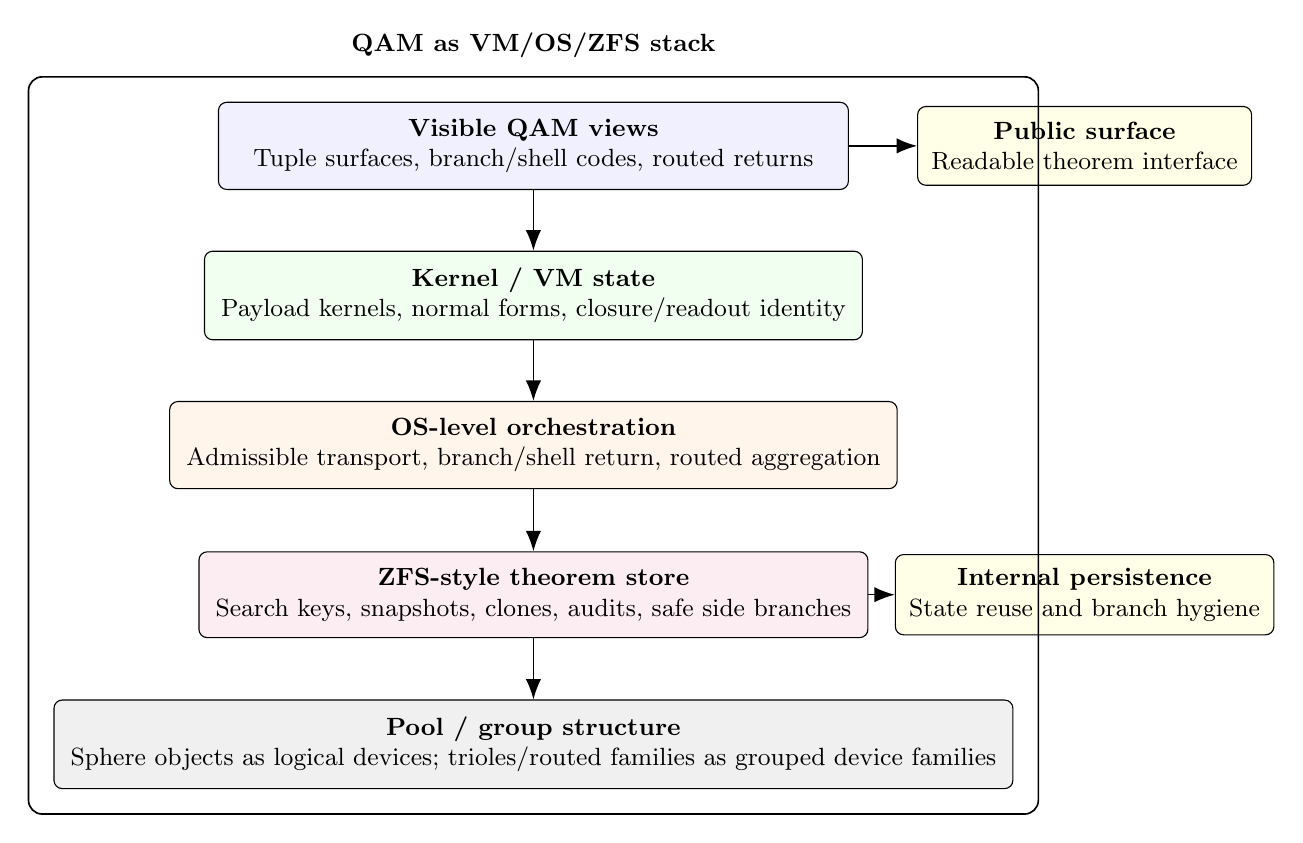
\begin{tikzpicture}[
  font=\small,
  mainbox/.style={draw, rounded corners=3pt, align=center, minimum width=8.0cm, minimum height=1.05cm, inner sep=6pt},
  sidebox/.style={draw, rounded corners=3pt, align=center, minimum width=3.9cm, minimum height=1.0cm, inner sep=5pt},
  arr/.style={-{Latex[length=2.6mm]}, line width=0.5pt}
]

\node[mainbox, fill=blue!6]   (visible)  at (0,0)   {\textbf{Visible QAM views}\\Tuple surfaces, branch/shell codes, routed returns};
\node[sidebox, fill=yellow!10] (public)   at (7.0,0)   {\textbf{Public surface}\\Readable theorem interface};
\node[mainbox, fill=green!6]  (kernel)   at (0,-1.9) {\textbf{Kernel / VM state}\\Payload kernels, normal forms, closure/readout identity};
\node[mainbox, fill=orange!8] (os)       at (0,-3.8) {\textbf{OS-level orchestration}\\Admissible transport, branch/shell return, routed aggregation};
\node[mainbox, fill=purple!7] (store)    at (0,-5.7) {\textbf{ZFS-style theorem store}\\Search keys, snapshots, clones, audits, safe side branches};
\node[sidebox, fill=yellow!10] (internal) at (7.0,-5.7) {\textbf{Internal persistence}\\State reuse and branch hygiene};
\node[mainbox, fill=gray!12]  (pool)     at (0,-7.6) {\textbf{Pool / group structure}\\Sphere objects as logical devices; trioles/routed families as grouped device families};

\draw[arr] (visible) -- (kernel);
\draw[arr] (kernel) -- (os);
\draw[arr] (os) -- (store);
\draw[arr] (store) -- (pool);
\draw[arr] (visible.east) -- (public.west);
\draw[arr] (store.east) -- (internal.west);

\node[draw, rounded corners=5pt, fit=(visible)(kernel)(os)(store)(pool), inner sep=9pt, line width=0.6pt] (stackfit) {};
\node[above=0.15cm of stackfit.north, fill=white, inner sep=2pt] {\textbf{QAM as VM/OS/ZFS stack}};
\end{tikzpicture}%
}\caption{Graphical reading of the current QAM export as a virtual-machine/OS stack with a ZFS-style structural store. Visible tuple surfaces provide the public theorem interface; exposed payload kernels and kernel normal forms provide the later machine-state identity; snapshots, clones, search keys, and audits manage the internal proof store without changing the visible public QAM syntax.}
\label{fig:qam-vm-os-zfs}
\end{figure}

\begin{remark}[Why the ZFS analogy is structurally useful here]\label{rem:qam-zfs-utility}
The ZFS-style reading is not meant as decorative metaphor. It isolates four practical gains already visible in the present file. First, equal kernel classes can later be treated as mirror-like state reuse rather than as repeatedly independent visible tuple surfaces. Second, the deferred kernel-first path already behaves like copy-on-write: experimental compression statements are developed beside the active tuple proofs without rewriting the active line. Third, checkpoints, audits, and activation criteria behave like snapshots and scrub rules for the theorem store, since they record exactly which deferred branches are stable and which still remain non-authoritative. Fourth, once kernel normal forms and search keys are in place, repeated branch/shell/routed return families can be indexed and deduplicated as one structural graph beneath a readable tree-shaped theorem presentation. This is precisely why the systems analogy deserves a more prominent place next to the public QAM extraction itself.
\end{remark}

\begin{remark}[Current scope of the VM/OS/ZFS view]\label{rem:qam-vm-os-scope}
In the inherited v3.16.0 public-shape layer this systems view remains explanatory and organizational. It does not introduce a second formal semantics, and it does not yet activate RAID-like reconstruction as an active theorem rule. The present mathematically justified gains at that inherited layer are the mirror-like reuse of equal kernel classes, the snapshot/clone logic of active versus deferred proof branches, and the content-addressed search-key discipline attached to kernel normal forms. The v3.34.0 extension below activates only a guarded store-and-array vocabulary over the already available QAM/MML/MMA interface. It still does not turn mirror, stripe, parity, or repair language into an OP-closure certificate.
\end{remark}


\subsection*{QAM/MML/MMA store layer and Sphaera array extension}
\begin{quote}\small
\noindent\textbf{Status.} \emph{Active v3.34.0 infrastructure block; no OP closure claim.}\par
\noindent\textbf{Block function.} This block internalizes the earlier ZFS/RAID analogy. QAM supplies the object store, MML supplies the store and array instructions, MMA supplies the execution/readout semantics, and finite Sphaera arrays supply guarded multi-object redundancy, comparison, and residual/parity witnesses.
\end{quote}

The preceding systems view should no longer be read merely as an external metaphor. At the present local layer it becomes a controlled internal interface. The point is not to claim that the Companion has already become a universal computer, nor that OP~1/4 or OP~5(B) have closed. The point is narrower and useful: the same QAM/MML/MMA machinery that already records objects, instructions, and route-faithful execution can also write the persistence layer in which several Sphaera objects are stored, compared, snapshotted, scrubbed, and carried as a guarded array.

\paragraph{Human reading.}
A single Sphaera object is now treated like one protected theorem-state device. Several Sphaera objects may be grouped into an array. In mirror mode, different objects carry the same structural content through different admissible views. In stripe mode, one larger proof or diagnostic object is distributed over several component stores. In parity/residual mode, an additional Sphaera object carries the difference, obstruction, or orthogonal control witness attached to the other components.

\paragraph{LLM/audit reading.}
The layer below gives stable machine-readable handles for store state, snapshot, clone, rollback, scrub, array creation, mirror, stripe, parity, and array snapshot. These handles are not theorematic shortcuts. They are audit contracts: each command must preserve address discipline, guard discipline, lineage discipline, and the non-certificate status unless a separate explicit theorem later discharges that status.

\begin{figure}[H]
\centering
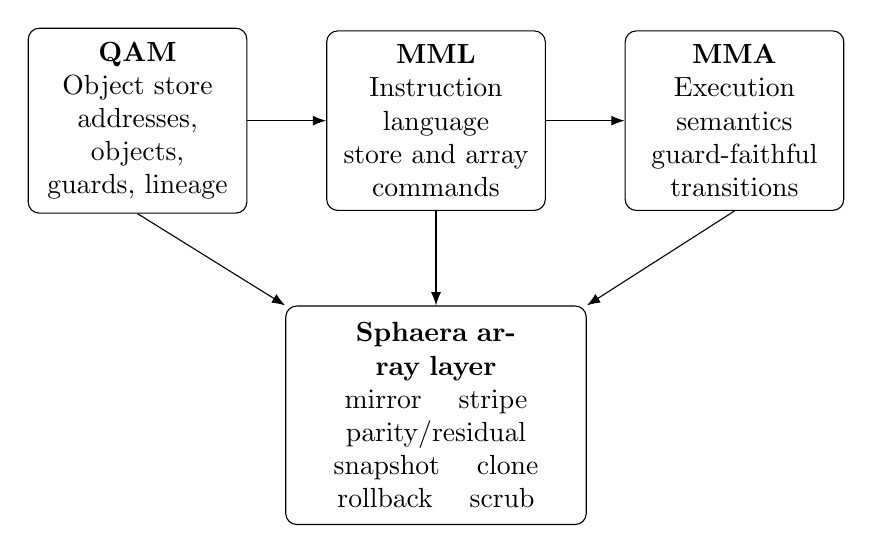
\begin{tikzpicture}[
  node distance=8mm and 10mm,
  box/.style={draw, rounded corners, align=center, inner sep=5pt, text width=0.2\textwidth},
  bigbox/.style={draw, rounded corners, align=center, inner sep=6pt, text width=0.28\textwidth},
  >=Latex
]
\node[box] (qam) {\textbf{QAM}\\Object store\\addresses, objects, guards, lineage};
\node[box, right=of qam] (mml) {\textbf{MML}\\Instruction language\\store and array commands};
\node[box, right=of mml] (mma) {\textbf{MMA}\\Execution semantics\\guard-faithful transitions};
\node[bigbox, below=12mm of mml] (array) {\textbf{Sphaera array layer}\\mirror \quad stripe \quad parity/residual\\snapshot \quad clone \quad rollback \quad scrub};
\draw[->] (qam) -- (mml);
\draw[->] (mml) -- (mma);
\draw[->] (qam.south) -- (array.north west);
\draw[->] (mml.south) -- (array.north);
\draw[->] (mma.south) -- (array.north east);
\end{tikzpicture}
\caption{Reader-facing systems map for the QAM/MML/MMA store-array extension. QAM supplies the stored object layer, MML supplies the allowed store and array commands, MMA supplies the guarded execution semantics, and the Sphaera array layer packages mirror, stripe, and parity/residual modes together with snapshot, clone, rollback, and scrub operations.}
\label{fig:qam-mml-mma-store-array-map}
\end{figure}

\begin{table}[H]
\centering
\small
\begin{tabular}{>{\raggedright\arraybackslash}p{0.18\textwidth} >{\raggedright\arraybackslash}p{0.26\textwidth} >{\raggedright\arraybackslash}p{0.26\textwidth} >{\raggedright\arraybackslash}p{0.20\textwidth}}
\toprule
\textbf{Layer} & \textbf{Human reading} & \textbf{LLM/audit reading} & \textbf{Typical outputs}\\
\midrule
QAM & protected object store & typed address/object/guard/ledger state & store state, snapshot anchor\\
MML & allowed store and array actions & finite instruction alphabet & \texttt{STORE}, \texttt{SNAPSHOT}, \texttt{PARITY}\\
MMA & how commands really act & deterministic guarded transition semantics & continue / halt / reject / guard\\
Sphaera array & several Sphaera objects coupled as one working array & finite guarded family with cross-sphere guards and parity witnesses & mirror, stripe, parity/residual, scrub\\
\bottomrule
\end{tabular}
\caption{Compact overview table for the store-array layer. This separates reader intuition from the audit contract without changing the theorematic status of the block.}
\label{tab:qam-mml-mma-store-array-overview}
\end{table}


\begin{definition}[QAM store state]\label{def:qam-store-state}
A \emph{QAM store state} is a finite guarded tuple
\[
  \mathcal S_n
  :=
  (\mathcal A_n,\mathcal O_n,\mathcal R_n,\mathcal G_n,\mathcal L_n),
\]
where \(\mathcal A_n\) is the finite address/tag domain, \(\mathcal O_n\) is the finite family of stored QAM objects, \(\mathcal R_n\) is the finite relation/link register between stored objects, \(\mathcal G_n\) is the finite guard register, and \(\mathcal L_n\) is the finite lineage/audit ledger. The state is \emph{admissible} if every ledger pointer lands in \(\mathcal A_n\), every relation in \(\mathcal R_n\) uses stored addresses, and every active guard in \(\mathcal G_n\) is satisfied by the displayed objects and relations.
\end{definition}

\begin{definition}[Store instruction alphabet]\label{def:mml-store-instructions}
The local MML store alphabet is the finite instruction family
\[
\begin{split}
  \mathcal I_{\mathrm{store}}
  :=\{&\texttt{STORE},\texttt{LINK},\texttt{SNAPSHOT},\texttt{CLONE},\texttt{ROLLBACK},\texttt{SCRUB},\texttt{MERGE\_CAND},\texttt{EXPORT}\}.
\end{split}
\]
Here \(\texttt{STORE}\) writes an object to an address, \(\texttt{LINK}\) writes a relation, \(\texttt{SNAPSHOT}\) freezes an admissible state, \(\texttt{CLONE}\) opens a guarded side branch from a snapshot, \(\texttt{ROLLBACK}\) returns to a recorded snapshot, \(\texttt{SCRUB}\) checks the guards and lineage, \(\texttt{MERGE\_CAND}\) proposes a guarded merge candidate, and \(\texttt{EXPORT}\) exposes a readout surface. None of these instructions is allowed to manufacture a theorematic certificate by syntax alone.
\end{definition}

\begin{definition}[MMA store transition semantics]\label{def:mma-store-transition}
The local MMA store semantics is a partial deterministic transition map
\[
  \delta_{\mathrm{store}}
  :
  \mathcal S_n\times\mathcal I_{\mathrm{store}}
  \dashrightarrow
  \mathcal S_{n+1}\times
  \{\mathsf{continue},\mathsf{halt},\mathsf{reject},\mathsf{guard}\}.
\]
It is \emph{guard-faithful} if every defined transition either preserves admissibility of the resulting store or returns the status \(\mathsf{guard}\) together with a defect entry in the ledger. It is \emph{lineage-faithful} if each defined transition records enough ledger data to identify its source state, instruction, guard status, and output state.
\end{definition}

\begin{definition}[Guarded snapshot and clone]\label{def:qam-store-snapshot}
For an admissible QAM store \(\mathcal S_n\), a \emph{guarded snapshot} is a tuple
\[
  \operatorname{snap}(\mathcal S_n)
  :=
  (\mathcal S_n,\chi_n,\lambda_n),
\]
where \(\chi_n\) is a finite integrity witness for the address, relation, guard, and ledger registers, and \(\lambda_n\) is a lineage anchor. A \emph{clone} of \(\operatorname{snap}(\mathcal S_n)\) is a new working state \(\mathcal S'_n\) with the same stored content and a new branch tag in the ledger. The clone is not a new theorem; it is a new guarded working branch from the same stored state.
\end{definition}

\begin{proposition}[Snapshot stability of admissible QAM stores]\label{prop:qam-store-snapshot-stability}
Every admissible finite QAM store state admits a guarded snapshot in the sense of Definition~\ref{def:qam-store-snapshot}. If the MMA store semantics is guard-faithful and lineage-faithful, then \(\texttt{SNAPSHOT}\), \(\texttt{CLONE}\), and \(\texttt{ROLLBACK}\) preserve the distinction between stored mathematical objects and release/audit metadata.
\end{proposition}

\begin{proof}
Since the address, object, relation, guard, and ledger registers are finite, their displayed state can be recorded as a finite tuple together with a finite integrity witness and a lineage anchor. This gives \(\operatorname{snap}(\mathcal S_n)\). Guard-faithfulness prevents a failed guard from being silently stored as an admissible state, and lineage-faithfulness records the source and branch data. Thus snapshot, clone, and rollback may move between recorded store states, but they do not promote a release label, branch label, or audit label into the mathematical object language.
\end{proof}

\begin{definition}[Sphaera array]\label{def:sphaera-array}
A \emph{Sphaera array} is a finite guarded family
\[
  \mathbb S_n
  :=
  \bigl((\mathcal S_n^{(1)},\ldots,\mathcal S_n^{(k)});\Gamma_n,\Pi_n,\Lambda_n\bigr),
  \qquad k\ge 1,
\]
where each \(\mathcal S_n^{(i)}\) is an admissible QAM store state, \(\Gamma_n\) is the cross-sphere guard register, \(\Pi_n\) is the parity/residual witness register, and \(\Lambda_n\) is the array-level lineage ledger. The array is admissible if all component stores are admissible and all cross-sphere guards in \(\Gamma_n\) are satisfied.
\end{definition}

\begin{definition}[Array instruction alphabet]\label{def:sphaera-array-instructions}
The local MML array alphabet is
\[
\begin{aligned}
  \mathcal I_{\mathrm{array}}
  :=\{&\texttt{ARRAY\_CREATE},\texttt{MIRROR},\texttt{STRIPE},\texttt{PARITY},\\
       &\texttt{SCRUB\_ARRAY},\texttt{REPAIR\_CAND},\texttt{SNAPSHOT\_ARRAY}\}.
\end{aligned}
\]
The command \(\texttt{REPAIR\_CAND}\) intentionally returns a candidate repair surface, not an automatic mathematical repair theorem. The command \(\texttt{PARITY}\) records a residual or orthogonal control witness, not a proof that the residual vanishes.
\end{definition}

\begin{definition}[Mirror, stripe, and parity modes]\label{def:sphaera-array-modes}
Let \(\mathbb S_n\) be an admissible Sphaera array.
\begin{enumerate}[leftmargin=2em]
  \item In \emph{mirror mode}, two component stores \(\mathcal S_n^{(i)}\) and \(\mathcal S_n^{(j)}\) are coupled by a cross-guard requiring equality of the relevant closure-compatible readout, even if the visible store presentations differ.
  \item In \emph{stripe mode}, an object \(X\) is stored as a finite guarded decomposition \(X\rightsquigarrow(X_1,\ldots,X_k)\), with each stripe \(X_i\) stored in a specified component and with a reconstruction witness recorded in \(\Pi_n\).
  \item In \emph{parity/residual mode}, one component or register stores a residual witness \(P\) for a guarded comparison of other components. The condition \(P=0\), if ever needed, must be proved separately; it is not asserted by the existence of the parity register.
\end{enumerate}
\end{definition}

\begin{definition}[Triadic Sphaera array]\label{def:triadic-sphaera-array}
A \emph{triadic Sphaera array} is an admissible Sphaera array of the form
\[
  \mathbb S_n^{ABC}
  :=
  (\mathcal S_A,\mathcal S_B,\mathcal S_C;\Gamma_{ABC},\Pi_{ABC},\Lambda_{ABC})
\]
in which \(\mathcal S_A\) and \(\mathcal S_B\) carry two active readout or probe-facing stores, while \(\mathcal S_C\) carries the orthogonal residual/parity witness. The guard register records the structural condition that \(\mathcal S_C\) is read orthogonally to the active \(A/B\) coupling channel and that the HC/MM readout of the array preserves the inherited route tag.
\end{definition}

\begin{proposition}[Guarded array snapshot]\label{prop:sphaera-array-snapshot}
Every admissible finite Sphaera array admits a guarded array snapshot
\[
  \operatorname{snap}_{\mathrm{arr}}(\mathbb S_n)
  :=
  \bigl(\mathbb S_n,(\chi_n^{(1)},\ldots,\chi_n^{(k)}),\chi_n^{\Gamma},\chi_n^{\Pi},\lambda_n^{\mathrm{arr}}\bigr),
\]
preserving component stores, cross-sphere guards, parity/residual witnesses, and array lineage.
\end{proposition}

\begin{proof}
Apply Proposition~\ref{prop:qam-store-snapshot-stability} to each finite component store. Since the cross-guard, parity/residual, and array-ledger registers are also finite, record their integrity witnesses and one array lineage anchor. The resulting tuple is a guarded array snapshot. It records the array state without adding an OP-closure certificate and without changing any component object into metadata.
\end{proof}

\begin{proposition}[Finite array scrub]\label{prop:sphaera-array-scrub}
For every finite Sphaera array there is a deterministic scrub procedure
\[
  \operatorname{scrub}_{\mathrm{arr}}(\mathbb S_n)
  \in
  \{\mathsf{pass},\mathsf{fail}\}\times\mathcal D_n,
\]
where \(\mathcal D_n\) is a finite defect register. The scrub passes exactly when all component-store guards, cross-sphere guards, parity/residual registrations, and lineage pointers pass their finite checks.
\end{proposition}

\begin{proof}
The component store registers, cross-guard register, parity/residual register, and lineage ledger are finite by definition. A deterministic scrub checks them in a fixed order and records every failed check in \(\mathcal D_n\). If no failed check is recorded, the result is \(\mathsf{pass}\); otherwise it is \(\mathsf{fail}\) with the finite defect register. No repair or closure claim is produced by this test.
\end{proof}

\begin{theorem}[QAM/MML/MMA Sphaera array layer]\label{thm:qam-mml-mma-sphaera-array-layer}
The QAM/MML/MMA stack admits a conservative Sphaera array layer in the following sense. Given finite admissible QAM stores, the store instruction alphabet of Definition~\ref{def:mml-store-instructions}, the array instruction alphabet of Definition~\ref{def:sphaera-array-instructions}, and guard-faithful lineage-faithful MMA transition semantics, one obtains finite guarded snapshots, finite array snapshots, and deterministic array scrub surfaces. These surfaces preserve stored mathematical objects, cross-sphere guards, residual/parity witnesses, and audit lineage without manufacturing an OP-closure certificate.
\end{theorem}

\begin{proof}
The store part follows from Definitions~\ref{def:qam-store-state}--\ref{def:qam-store-snapshot} and Proposition~\ref{prop:qam-store-snapshot-stability}. The array part follows by grouping finitely many admissible stores as in Definition~\ref{def:sphaera-array}, assigning finite cross-guards, finite parity/residual witnesses, and a finite lineage ledger, and then applying Propositions~\ref{prop:sphaera-array-snapshot} and~\ref{prop:sphaera-array-scrub}. The last clause follows from the explicit non-certificate restrictions in Definitions~\ref{def:mml-store-instructions}, \ref{def:sphaera-array-instructions}, and \ref{def:sphaera-array-modes}: mirror, stripe, parity, scrub, and repair-candidate language records infrastructure and diagnostic data only. It does not assert vanishing residuals or OP closure.
\end{proof}

\begin{corollary}[RAID-like reading without RAID overclaim]\label{cor:sphaera-array-raid-reading}
The Sphaera array layer supports a RAID-like reading: mirror mode corresponds to redundant closure-compatible readout, stripe mode corresponds to guarded distribution of a larger object over several component stores, and parity/residual mode corresponds to an explicit diagnostic witness for cross-component mismatch. This reading is internal to QAM/MML/MMA, but it remains weaker than technical RAID reconstruction and weaker than any OP-closure theorem.
\end{corollary}

\begin{proof}
This is only a translation of Definition~\ref{def:sphaera-array-modes} into systems language. The mathematical content remains the guarded store, snapshot, array, parity/residual, and scrub structure already proved above.
\end{proof}

\begin{remark}[Tool extraction from the Sphaera array layer]\label{rem:sphaera-array-tool-extraction}
The new layer extracts four reusable tools for later Companion revisions.
\begin{enumerate}[leftmargin=2em]
  \item \textbf{Snapshot tool.} Freeze one admissible QAM store without changing the mathematical object language.
  \item \textbf{Clone/rollback tool.} Open or return from a guarded branch while preserving lineage and non-certificate status.
  \item \textbf{Array-scrub tool.} Test several Sphaera stores, cross-guards, and residual witnesses as one finite diagnostic surface.
  \item \textbf{Triadic parity tool.} Use a third, orthogonal Sphaera object as residual/parity witness for a two-store active coupling.
\end{enumerate}
These tools are deliberately infrastructural. Their value is that later OP-facing work can compare, branch, and roll back several coupled Sphaera objects without confusing state persistence with theorematic closure.
\end{remark}

\begin{remark}[Human/LLM interface gain]\label{rem:sphaera-array-human-llm-gain}
For a human reader, the store-array layer explains why the Companion keeps snapshots, historical witnesses, audit ledgers, and branch restrictions so visibly: they are the theorem-store equivalent of protected state persistence. For an LLM reader, the same layer supplies exact handles: \(\mathcal S_n\) for one store, \(\mathbb S_n\) for an array, \(\Gamma_n\) for cross-guards, \(\Pi_n\) for parity/residual witnesses, and \(\Lambda_n\) for lineage. This is the intended compromise between human readability and machine precision.
\end{remark}


\subsection*{Pre-v4 QAM Hilbert-shift and guarded mixed readouts}
\begin{quote}\small
\noindent\textbf{Status.} \emph{Pre-v4 preparation layer only.} The inherited QAM tuple tags are not globally migrated in Version~\docversion{}. The block below records the conservative Hilbert-shift plan, the mixed-readout package discipline, and an optional binary mask registry for future readout classification.
\end{quote}

The index-0 issue is now treated explicitly. In the inherited QAM tuple namespace, tag 0 occurs as an inhabited constructor tag, for instance on visible tuple surfaces of the form $\langle 0,a\rangle$. In a Boolean mask or IPv4-like readout registry, however, value 0 must mean no active kind. The next major QAM migration should therefore not identify these two uses. The preparation layer below records the planned Hilbert-hotel shift that can free tag 0 in the future while preserving the payloads and proofs.

\begin{definition}[QAM Hilbert-shift plan]\label{def:qam-hilbert-shift-plan}
Let $\mathcal K_{\mathrm{old}}$ be the inherited finite QAM tuple-tag namespace used by the current public syntax, and let $\mathcal K_{\mathrm{new}}$ be a shifted namespace with tag 0 reserved for the empty/no-active-kind marker. The planned Hilbert-shift is the constructor-level map
\[
  H_{\mathrm{QAM}}(\langle i,x_1,\ldots,x_m\rangle)
  :=
  \langle i+1,x_1,\ldots,x_m\rangle.
\]
It shifts only the constructor tag. It does not change the stored payload $(x_1,\ldots,x_m)$, the intended constructor distinction, or any mathematical content carried by the payload.
\end{definition}

\begin{definition}[Pre-v4 reserved-zero discipline]\label{def:pre-v4-reserved-zero-discipline}
The preparation line distinguishes two uses of zero.
\begin{enumerate}[leftmargin=2em]
  \item In the inherited v3.x tuple syntax, tag 0 remains an inhabited tuple tag wherever the old QAM definitions still use it.
  \item In the planned v4 shifted namespace and in every binary mask registry, tag or mask value 0 is reserved for empty, undefined, or no active kind.
\end{enumerate}
No Version~\docversion{} statement may silently replace the first convention by the second. Any global replacement is reserved for a later v4 migration theorem.
\end{definition}

\begin{proposition}[Conservative shape of the QAM Hilbert-shift]\label{prop:qam-hilbert-shift-conservative-shape}
Suppose a finite QAM sublanguage is translated by $H_{\mathrm{QAM}}$ and every constructor predicate, admissibility predicate, readout predicate, and closure-relevant predicate is translated by the same tag shift. Then the translated sublanguage is a conservative reindexing of the old one: payloads, constructor distinctions, admissibility status, readout compatibility, and closure-relevant truth values are preserved under the translation.
\end{proposition}

\begin{proof}
The map $H_{\mathrm{QAM}}$ is injective on constructor tags and leaves all payload coordinates unchanged. A constructor predicate in the shifted namespace is defined to hold exactly when the corresponding old predicate holds before applying the shift. The same translation is imposed on admissibility, readout, and closure-relevant predicates. Thus every proof step that used only constructor distinction, payload data, admissibility, readout compatibility, or closure-relevant class data has an isomorphic shifted proof step. The proposition records the required conservativity shape for a later v4 migration; it does not perform the global migration here.
\end{proof}

\begin{definition}[Guarded mixed QAM readout]\label{def:guarded-mixed-qam-readout}
A \emph{guarded mixed QAM readout} is a finite derived package
\[
  R_{\mathrm{mix}}
  :=
  (r_1,\ldots,r_m;\Gamma_{\mathrm{mix}},\mu,J_{\mathrm{mix}},\sigma_{\mathrm{mix}}),
\]
where each $r_i$ is an already admissible component readout on its own allowed QAM kind, $\Gamma_{\mathrm{mix}}$ is a finite guard package, $\mu$ is a finite aggregation map on component readout values, $J_{\mathrm{mix}}$ is the closure-factor map for the aggregate, and $\sigma_{\mathrm{mix}}$ records the theorematic status. It is admissible only when all component readouts are admissible and the aggregation map does not identify non-equivalent closure-relevant classes.
\end{definition}

\begin{definition}[Binary mask registry for mixed readouts]\label{def:binary-mask-registry-mixed-readouts}
A \emph{binary mask registry} for mixed QAM readouts assigns to each inhabited readout kind a nonzero power-of-two bit
\[
  \beta_j = 2^j,
  \qquad j\ge 0,
\]
and reserves mask value 0 for no active kind. A mixed-readout mask is a finite Boolean OR of active kind bits. Boolean AND tests whether a component kind is present, XOR records symmetric difference between two masks, and complement is allowed only relative to a fixed finite mask universe $\Omega$.
\end{definition}

\begin{proposition}[Mixed readout factorization]\label{prop:mixed-readout-factorization}
Let $R_{\mathrm{mix}}$ be a guarded mixed QAM readout whose component readouts $r_i$ are closure-compatible. If the aggregation map $\mu$ factors through the component closure-factor maps and $J_{\mathrm{mix}}$ factors through the resulting aggregate class, then $R_{\mathrm{mix}}$ is closure-compatible.
\end{proposition}

\begin{proof}
Closure-compatible component readouts identify no closure-relevant distinction beyond their component class maps. Since $\mu$ factors through those class maps, it can only aggregate already class-level data. Since $J_{\mathrm{mix}}$ factors through that aggregate class, the mixed readout cannot introduce a new closure-relevant distinction that was invisible to the component closure classes. Therefore the mixed package is closure-compatible. The argument uses only factorization and guards; it does not introduce primitive mixed tensors.
\end{proof}

\begin{remark}[v4 migration trigger]\label{rem:v4-qam-migration-trigger}
The full replacement of the inherited tuple tags by the shifted tags is intentionally not a Version~\docversion{} operation. It changes the visible QAM object-language namespace and therefore belongs to a major version. Version~\docversion{} only records why the shift is useful, what the conservative proof obligation looks like, and how mixed readouts can already be treated as derived packages without forcing the migration.
\end{remark}


% ============================================================================
% Quantum Sphaera Companion v3.35.0-r03 insertion patch
% Two-sided structural tensor notation for QAM/MML/MMA readouts
%
% Intended insertion point:
%   In the active-core source, place this block after the short QAM/MML/MMA
%   reader-orientation / pre-v4 QAM preparation material, and before any
%   broad theorematic QAM continuation.  In older sources the closest safe
%   anchor is after the remark "QAM normalization guide".
%
% Scope:
%   Conservative notation/compression layer only.  This is not the separate
%   pedagogical reader manual paper; that manual remains a future standalone
%   companion/guide document.
% ============================================================================

\subsection*{Two-sided structural tensor notation for QAM/MML/MMA readouts}
\begin{quote}\small
\noindent\textbf{Status.} \emph{Active notation and compression layer; not a new tensor calculus and not a new closure criterion.}\par
\noindent\textbf{Block function.} This block records the narrow two-sided tensor grammar used to separate readout-side, structure-side, comparison-side, and mask-side roles in later QAM/MML/MMA expressions.  It is included here as a conservative technical layer only.  A fuller pedagogical reader manual for the notation is intentionally kept as a separate future paper or companion guide.
\end{quote}

The QAM/MML/MMA line repeatedly alternates between four roles: frame-side readout, structure-side action, comparison of active channels, and compatibility testing of readout or mask modes.  The following notation is introduced only to make those roles visible in the formula syntax.  It does not replace classical tensor calculus and it does not turn every displayed expression into a new primitive tensor object.

\begin{definition}[Two-sided structural tensor interface]\label{def:two-sided-structural-tensor-interface}
A \emph{two-sided structural tensor display} is a tensor-like expression in which a structural object may carry front-side and back-side indices, written schematically as
\[
{}^{A}{}_{B}\mathcal{T}^{i}{}_{j}.
\]
The front indices \({}^{A}{}_{B}\) record the left-sided or readout-facing interface: frame, observer, language, readout, or external addressing data.  The back indices \({}^{i}{}_{j}\) record the right-sided or structure-facing interface: action, transport, field, operator, or internal structural data.  Thus the display is read as a typed structural interface rather than as a mere component array.
\end{definition}

\begin{definition}[Admissible contractions and comparisons]\label{def:two-sided-admissible-contractions}
The two-sided notation obeys the following contraction discipline.
\begin{enumerate}[leftmargin=2em]
  \item \textbf{Classical action/readout.} Ordinary upper--lower contraction remains unchanged.  If
  \[
  A_\mu\,{}^\mu\mathcal{T}_\nu\,B^\nu
  \]
  is well-defined, it is read as a classical action, evaluation, or sandwich readout: first apply the structure-facing operation to \(B\), then read the result by \(A\).
  \item \textbf{Active--active comparison.} Two upper indices are not contracted as a raw Einstein sum.  They may only be compared through an explicitly declared comparison tensor, for instance
  \[
  G_{\alpha\beta}X^\alpha Y^\beta .
  \]
  This means active structural comparison, such as angle, distance, coupling strength, orthogonality, channel similarity, or residual size.
  \item \textbf{Passive--passive comparison.} Two lower indices are likewise not contracted raw.  They may only be compared through an explicitly declared dual comparison tensor, for instance
  \[
  G^{\alpha\beta}\omega_\alpha\eta_\beta .
  \]
  This means comparison of readout forms, observer modes, measurement channels, or passive projections.
  \item \textbf{Mask and selector compatibility.} Boolean, finite, or mask-like compatibility tests must be carried by an explicit selector tensor, for instance
  \[
  \chi_{mn}R^mS^n .
  \]
  This expression says that readout modes \(m\) and \(n\) are first tested for admissible compatibility by \(\chi\), and only compatible contributions are admitted to the mixed readout.
\end{enumerate}
\end{definition}

\begin{remark}[Conservative reading rule]\label{rem:two-sided-conservative-reading-rule}
The two-sided notation is conservative because the only unchanged contraction is the classical upper--lower action/readout contraction.  Same-variance pairings are not silently added to the calculus; they are admitted only when a comparison tensor or selector tensor has been declared.  Hence every two-sided display must be expandable into ordinary QAM-over-ZF role predicates together with explicit comparison or compatibility data.
\end{remark}

\begin{definition}[Guarded mixed QAM readout]\label{def:guarded-two-sided-mixed-qam-readout}
Let \(R^m\) and \(S^n\) be QAM readout modes and let \(\chi_{mn}\) be an explicit admissibility or compatibility selector.  A \emph{guarded mixed QAM readout} is a derived readout expression of the form
\[
\operatorname{Mix}_{\chi}(R,S)(x)
\quad\leadsto\quad
\chi_{mn}R^m(x)S^n(x),
\]
where the right-hand display is read with the contraction discipline of Definition~\ref{def:two-sided-admissible-contractions}.  The mixed readout is therefore not a new primitive QAM object.  It is a compatibility-filtered package of already admitted readout modes.
\end{definition}

\begin{remark}[Residual comparison grammar]\label{ex:two-sided-residual-comparison}
The live residual triple
\[
\rho=(\rho_{\mathrm{CL}},\rho_{\Theta},\rho_A)
\]
may be compressed into a residual-channel vector \(\rho^\alpha\).  Its total comparison size may then be written as
\[
\|\rho\|_G^2=G_{\alpha\beta}\rho^\alpha\rho^\beta .
\]
This is not a raw contraction of two upper indices.  It is the comparison of two active residual-channel entries through the declared comparison tensor \(G_{\alpha\beta}\).
\end{remark}

\begin{remark}[HC/MM sandwich grammar]\label{ex:two-sided-hc-mm-sandwich}
An HC/MM-mediated readout may be displayed schematically as
\[
{}^{R}{}_{\Omega}\mathcal{M}^{i}{}_{j},
\]
where the front side records the readout or observer-side interface and the back side records the structure-side transport or matrix action.  When paired with ordinary upper--lower indices, the expression remains an ordinary sandwich readout.  When two readout channels or two structure channels are compared, the comparison must be mediated by an explicitly named comparison tensor or selector.
\end{remark}

\begin{proposition}[Conservative expansion of two-sided displays]\label{prop:two-sided-conservative-expansion}
Every well-formed two-sided structural tensor display in the sense of Definitions~\ref{def:two-sided-structural-tensor-interface} and~\ref{def:two-sided-admissible-contractions} admits a conservative expansion into the inherited QAM-over-ZF language: front-side indices expand to readout/frame/language role data, back-side indices expand to structure/action/transport role data, classical upper--lower contractions remain ordinary action or evaluation clauses, and every same-variance pairing expands to an explicit comparison or compatibility predicate.
\end{proposition}

\begin{proof}
Erase the visual sidedness notation and retain its role data as ordinary QAM codes.  Front-side symbols become readout, frame, observer, or language tags.  Back-side symbols become structure, action, transport, or field tags.  Classical upper--lower contractions are left unchanged.  A same-variance display is well formed only if it contains a named comparison tensor or selector, and so it expands to the corresponding comparison or compatibility predicate.  No new primitive closure relation, admissibility relation, or theorematic certificate is introduced by this erasure.  The display is therefore a conservative abbreviation of already typed QAM-over-ZF data.
\end{proof}

\begin{remark}[LLM-facing role stability]\label{rem:two-sided-llm-role-stability}
For machine reading and LLM-assisted proof navigation, the notation functions as a syntactic guardrail.  The front/back split marks whether a symbol belongs to the readout-facing side or the structure-facing side, while the contraction discipline marks whether a formula is an action, a readout, a comparison, or a compatibility test.  This reduces the risk that a readout is mistaken for an operator, that a diagnostic comparison is mistaken for a proof of closure, or that a guarded mixed readout is mistaken for a new primitive tensor object.
\end{remark}

\begin{remark}[Use in the present release line]\label{rem:two-sided-present-release-use}
In the present v3.35.x line this notation should be used locally and sparingly: first for guarded mixed QAM readouts, residual/drift comparisons, HC/MM sandwich expressions, triadic orthogonality comparisons, and Boolean or mask-like compatibility tests.  A global rewrite of the whole Companion into the two-sided notation is not part of this release line.  The separate pedagogical reader manual may later explain the notation at a slower pace without enlarging the active theorem core.
\end{remark}


% ============================================================================
% Quantum Sphaera Companion v3.35.0-r03 insertion patch
% Two-sided tensor stability, mixed-readout normal form, and Boolean masks
%
% Scope:
%   Stabilization layer only.  This block makes the r02 notation explicitly
%   expandable back into QAM-over-ZF role data and records the mask/readout
%   grammar that will later help the v4 QAM reindexing.  It is not the separate
%   pedagogical reader-manual paper.
% ============================================================================

\subsection*{r03 stability layer: two-sided expansion, mixed-readout normal form, and Boolean masks}
\begin{quote}\small
\noindent\textbf{Status.} \emph{Conservative stabilization of the r02 notation layer; not a global rewrite, not a new tensor calculus, and not a closure theorem.}\par
\noindent\textbf{Block function.} This block fixes the exact erasure route from two-sided displays back to ordinary QAM-over-ZF role data, normalizes guarded mixed readouts, and states the Boolean selector grammar used by IPv4-like readout masks.  The separate reader manual remains a future standalone paper or guide.
\end{quote}

The r02 notation made readout-side, structure-side, comparison-side, and mask-side roles visible in formulas.  The present r03 step turns that notation into a safer tool by recording the normal forms that an audit reader or LLM reader should recover whenever a two-sided display appears.  The rule is intentionally asymmetric: notation may compress role data, but every compressed display must expand back into explicit role data before it can be used as proof content.

\begin{definition}[Two-sided role-erasure map]\label{def:r03-two-sided-role-erasure-map}
Let \(E\) be a well-formed two-sided structural tensor display in the sense of Definitions~\ref{def:two-sided-structural-tensor-interface} and~\ref{def:two-sided-admissible-contractions}.  Its \emph{role-erasure expansion}
\[
\mathfrak{E}_{\mathrm{role}}(E)
\]
is the ordinary QAM-over-ZF package obtained by replacing:
\begin{enumerate}[leftmargin=2em]
  \item every front-side index by an explicit readout, frame, observer, or language-role tag;
  \item every back-side index by an explicit structure, action, field, transport, or operator-role tag;
  \item every classical upper--lower contraction by the corresponding ordinary action/evaluation clause;
  \item every same-variance comparison by a named comparison predicate carrying its declared comparison tensor;
  \item every Boolean or selector occurrence by a finite compatibility predicate over the declared mask universe.
\end{enumerate}
This expansion is an erasure of notation only.  It does not erase guards, selectors, comparison tensors, branch restrictions, or provenance data.
\end{definition}

\begin{proposition}[Role-erasure normal form]\label{prop:r03-role-erasure-normal-form}
Every well-formed two-sided display \(E\) used in the v3.35.x line has a role-erasure expansion \(\mathfrak{E}_{\mathrm{role}}(E)\) whose clauses are built from already admitted QAM role predicates, admitted comparison data, admitted selector data, and ordinary finite tuple coding over ZF.  In particular, the two-sided display cannot by itself introduce a new primitive tensor kind, a new admissibility relation, or a new theorematic certificate.
\end{proposition}

\begin{proof}
Proceed by structural inspection of the display grammar.  Front/back sidedness contributes only role tags.  Ordinary upper--lower contraction is already part of the inherited action/readout grammar.  A same-variance pairing is well formed only when it contains an explicitly named comparison tensor or selector, hence it expands to a comparison or compatibility predicate rather than to an untyped Einstein contraction.  All finite lists of such clauses are QAM tuple-coded over the existing ZF substrate.  Therefore the two-sided syntax is conservative under role erasure.
\end{proof}

\begin{definition}[Guarded mixed-readout normal form]\label{def:r03-guarded-mixed-readout-normal-form}
A guarded mixed QAM readout is in \emph{r03 normal form} when it is presented as a finite package
\[
\mathcal R_{\mathrm{mix}}
=
\bigl(I,\{R_i\}_{i\in I},\Gamma_{\mathrm{mix}},\chi,\mu,J_{\mathrm{mix}}\bigr),
\]
where \(I\) is a finite index set, each \(R_i\) is an already admitted component readout, \(\Gamma_{\mathrm{mix}}\) is the inherited guard package, \(\chi\) is a finite selector or mask predicate over \(I\), \(\mu\) is an aggregation map defined only on selector-admissible component families, and \(J_{\mathrm{mix}}\) is the declared mixed readout surface.  A two-sided display such as
\[
\chi_{mn}R^mS^n
\]
is only an abbreviation for this finite package in the binary case \(I=\{m,n\}\).
\end{definition}

\begin{proposition}[Mixed-readout normal-form expansion]\label{prop:r03-mixed-readout-normal-form-expansion}
Every guarded mixed readout admitted by Definition~\ref{def:guarded-two-sided-mixed-qam-readout} expands to an r03 guarded mixed-readout normal form in the sense of Definition~\ref{def:r03-guarded-mixed-readout-normal-form}.  Conversely, every r03 guarded mixed-readout normal form may be displayed in two-sided shorthand only after its guards, selector, aggregation map, and output surface have been declared.
\end{proposition}

\begin{proof}
The binary shorthand \(\chi_{mn}R^mS^n\) already names the two component readouts and the selector.  The surrounding QAM context supplies the inherited guard package, the admissible aggregation rule, and the declared output surface.  Collecting these data gives the normal-form tuple.  Conversely, starting from the normal-form tuple, one may suppress the finite package into two-sided shorthand only because the suppressed guard, selector, aggregation, and output data remain recoverable.  Thus the shorthand and the normal form are not different mathematical objects; the former is a compact notation for the latter.
\end{proof}

\begin{definition}[Boolean selector and mask grammar]\label{def:r03-boolean-selector-mask-grammar}
Fix a finite readout-kind universe \(\Omega=\{k_1,\dots,k_N\}\).  A \emph{Boolean selector mask} is a function
\[
\chi:\Omega\longrightarrow\{0,1\}
\]
or, equivalently, a finite bit mask whose value 0 denotes no active kind and whose nonzero bits denote active readout kinds.  The admissible Boolean operations are:
\begin{align*}
\chi_A\vee\chi_B &\quad\text{for union of active readout kinds,}\\
\chi_A\wedge\chi_B &\quad\text{for intersection or compatibility testing,}\\
\chi_A\oplus\chi_B &\quad\text{for diagnostic symmetric difference,}\\
\neg_{\Omega}\chi_A &\quad\text{for relative complement inside the fixed universe }\Omega.
\end{align*}
No absolute complement is used without first declaring \(\Omega\).  A selector expression may filter a readout package, but it does not alter the payload of any component readout.
\end{definition}

\begin{proposition}[Mask-filter conservativity]\label{prop:r03-mask-filter-conservativity}
Let \(\mathcal R_{\mathrm{mix}}\) be an r03 guarded mixed-readout normal form and let \(\chi\) be a Boolean selector mask over its finite readout-kind universe.  Applying \(\chi\) restricts the active component menu of \(\mathcal R_{\mathrm{mix}}\), but it does not change the underlying component payloads, the inherited guards, or the closure status of any component readout.
\end{proposition}

\begin{proof}
A selector mask is a finite predicate on the index universe.  It chooses which already declared component clauses are active in the aggregation domain.  It neither rewrites the component readouts nor changes their guard packages.  Hence any closure-compatible status used by the mixed package still has to come from the component readouts and the declared factorization map, not from the mask itself.
\end{proof}

\begin{remark}[LLM/audit role table]\label{rem:r03-llm-audit-role-table}
For later machine reading, the following table fixes the intended role parsing.  It is a local audit aid inside the Companion, not the separate pedagogical reader manual.
\begin{center}
\renewcommand{\arraystretch}{1.12}
\begin{tabular}{|p{0.28\textwidth}|p{0.34\textwidth}|p{0.25\textwidth}|}
\hline
\textbf{Displayed form} & \textbf{Intended role} & \textbf{Audit guard} \\
\hline
front-side indices & readout, frame, observer, language, or addressing side & expand to explicit QAM role tags \\
\hline
back-side indices & structure, action, field, transport, or operator side & expand to explicit QAM role tags \\
\hline
upper--lower contraction & classical action, evaluation, or sandwich readout & ordinary tensor/QAM readout clause \\
\hline
upper--upper via \(G_{\alpha\beta}\) & active structural comparison & no raw same-variance contraction \\
\hline
lower--lower via \(G^{\alpha\beta}\) & passive readout comparison & no raw same-variance contraction \\
\hline
\(\chi_{mn}\) or a mask bit & compatibility or activation selector & filter only; no new payload \\
\hline
\end{tabular}
\end{center}
\end{remark}

\begin{corollary}[r03 proof-neutrality of the tensor layer]\label{cor:r03-proof-neutrality-of-tensor-layer}
The r03 tensor-stability layer may be cited to shorten repeated readout/action/comparison/mask passages, but it may not be cited as an independent proof of closure, OP resolution, primitive mixed-tensor existence, or global QAM namespace migration.
\end{corollary}

\begin{proof}
By Propositions~\ref{prop:r03-role-erasure-normal-form}, \ref{prop:r03-mixed-readout-normal-form-expansion}, and~\ref{prop:r03-mask-filter-conservativity}, every r03 display reduces to already declared role data, normal-form mixed-readout data, and finite selector predicates.  The reduction supplies notation control only.  It does not add the missing theorematic hypotheses needed for closure, OP resolution, primitive mixed tensors, or v4 reindexing.
\end{proof}

\begin{remark}[Placement of the future reader manual]\label{rem:r03-reader-manual-placement}
The present block deliberately stays short and formal.  A slower reader manual may later explain the same grammar with diagrams, examples, and human-facing intuition, but that manual should remain a separate paper or guide so that the Active Core remains the governing proof line.
\end{remark}


% Quantum Sphaera Companion v3.35.0-r04 release-candidate insertion
% Release-candidate freeze/audit layer only.  No mathematical closure claim.

\subsection*{r04 release-candidate freeze audit for the pre-v4 QAM/tensor layer}
\addcontentsline{toc}{subsection}{r04 release-candidate freeze audit for the pre-v4 QAM/tensor layer}
\label{subsec:r04-release-candidate-freeze-audit-qam-tensor}

\noindent\textbf{Status.} \emph{Release-candidate audit layer only; no new theorematic certificate, no global QAM namespace migration, no primitive mixed tensor, and no OP closure.}\par
\noindent\textbf{Block function.} This r04 block freezes the r02/r03 notation and mixed-readout preparation layer for release-candidate review.  It records what must remain true when the Active Core is read together with the separate Historical Witness PDF.

\begin{definition}[r04 pre-v4 QAM/tensor release-candidate package]
\label{def:r04-pre-v4-qam-tensor-release-candidate-package}
The \emph{r04 pre-v4 QAM/tensor release-candidate package} consists of the following finite data:
\begin{enumerate}[label=(\roman*)]
  \item the inherited v3.34.0 public split-bundle baseline and its concept/version DOI record;
  \item the v3.35.0 short-abstract and extended-orientation architecture;
  \item the pre-v4 Hilbert-shift plan reserving global QAM tag migration for a later major version;
  \item the guarded mixed-readout discipline and optional binary mask registry;
  \item the r02 two-sided structural tensor notation;
  \item the r03 role-erasure, mixed-readout normal form, Boolean selector grammar, and proof-neutrality layer;
  \item the present r04 audit/handoff metadata saying that the Active Core is the governing proof line and that the Historical Witness PDF remains preserved proof memory.
\end{enumerate}
It is a packaging and audit object, not a closure object.
\end{definition}

\begin{proposition}[r04 release-candidate conservativity]
\label{prop:r04-release-candidate-conservativity}
The r04 pre-v4 QAM/tensor release-candidate package is conservative over the r03 tensor-stability layer with respect to theorematic content.  It may change release-candidate metadata, routing language, audit surfaces, and handoff wording, but it may not create any new OP certificate, global Hilbert-shift theorem, primitive mixed-tensor axiom, or replacement of the inherited QAM tuple namespace.
\end{proposition}

\begin{proof}
Each mathematical role introduced by r02 is erased by Definition~\ref{def:r03-two-sided-role-erasure-map} and normalized by Proposition~\ref{prop:r03-role-erasure-normal-form}.  Each mixed readout is expanded by Proposition~\ref{prop:r03-mixed-readout-normal-form-expansion}, and each Boolean mask action is restricted by Proposition~\ref{prop:r03-mask-filter-conservativity}.  The r04 package adds only release-candidate metadata and bundle-handoff statements around these already guarded objects.  Hence no new theorematic content is introduced.
\end{proof}

\begin{corollary}[r04 freeze-readiness condition]
\label{cor:r04-freeze-readiness-condition}
If the build audit reports no duplicate labels, no undefined references, no undefined citations, and no fatal LaTeX errors for both the Active Core and the Historical Witness, then Version~\docversion{} is structurally ready to be treated as a freeze candidate for the v3.35.0 pre-v4 QAM/tensor preparation release, subject only to the external release decision and any assigned Zenodo version DOI.
\end{corollary}

\begin{remark}[Reader-manual separation at r04]
\label{rem:r04-reader-manual-separation}
The pedagogical reader manual for the two-sided notation remains outside the Active Core.  It may later be written as a separate guide with diagrams, examples, and slower explanations.  The present Companion keeps only the compact formal grammar and the proof-neutrality guards needed by the governing proof line.
\end{remark}


% Quantum Sphaera Companion v3.35.0 release-final DOI insertion
% Release metadata only. No mathematical object is indexed by the DOI.

\subsection*{v3.35.0 DOI-bearing release freeze}
\addcontentsline{toc}{subsection}{v3.35.0 DOI-bearing release freeze}
\label{subsec:v3350-doi-bearing-release-freeze}

\noindent\textbf{Status.} \emph{Release-final metadata layer only; no new theorematic certificate, no global QAM namespace migration, no primitive mixed tensor, and no OP closure.}\par
\noindent\textbf{Version DOI.} The public version-specific Zenodo DOI for this release is
\[
  \href{https://doi.org/10.5281/zenodo.19750674}{10.5281/zenodo.19750674}.
\]
The Companion concept DOI remains \href{https://doi.org/10.5281/zenodo.19210728}{10.5281/zenodo.19210728}. The version DOI is release metadata only and is not a mathematical subscript, superscript, route tag, or proof object.

\begin{definition}[v3.35.0 release-final package]
\label{def:v3350-release-final-package}
The \emph{v3.35.0 release-final package} consists of the r04 release-candidate package of Definition~\ref{def:r04-pre-v4-qam-tensor-release-candidate-package}, the assigned public version DOI above, the Active Core PDF, the preserved Historical Witness PDF, the release manifest, checksums, audit report, Zenodo description, and release notes.  It is a release object, not a theorematic closure object.
\end{definition}

\begin{proposition}[v3.35.0 release-final conservativity]
\label{prop:v3350-release-final-conservativity}
The v3.35.0 release-final package is conservative over the r04 release-candidate package with respect to theorematic content.  DOI insertion, release-note generation, manifest creation, checksum creation, and Zenodo-description preparation do not create any new OP certificate, global QAM Hilbert-shift theorem, primitive mixed-tensor axiom, or replacement of the inherited QAM tuple namespace.
\end{proposition}

\begin{proof}
By Proposition~\ref{prop:r04-release-candidate-conservativity}, the r04 package is conservative over r03.  The present layer adds only release metadata and publication packaging: the version DOI, release file names, manifest/checksum records, audit report, Zenodo description, and release notes.  None of these objects changes the payload of any QAM role, tensor grammar, mask selector, mixed readout, or OP-facing proof obligation.  Hence theorematic content is unchanged.
\end{proof}


\begin{remark}[How the systems view reads the present visual diagnostics]\label{rem:qam-vm-os-visuals}
The same stack view also explains why Appendix~C may carry highly visible packet, Julia-boundary, and frame-flicker diagnostics without turning those figures into primary closure axioms. In the systems reading, such figures live on the visible-view layer: they are auditable readout surfaces of one and the same transported channel, not independent kernel identities. This is exactly why the OP~5 packet/breathing/frame-flicker block and the Julia-boundary block belong naturally to the same document architecture as the deferred kernel store. The figures make visible what the current theorem store is tracking, while closure itself still remains controlled at the structural layer beneath the pictures.
\end{remark}


\begin{remark}[QAM/systems crosswalk for the present document]\label{rem:qam-vm-os-crosswalk}
The present document uses the systems analogy in a disciplined layer-by-layer way. The following crosswalk fixes the intended reading.
\begin{center}
\renewcommand{\arraystretch}{1.12}
\begin{tabular}{|p{0.29\textwidth}|p{0.28\textwidth}|p{0.31\textwidth}|}
\hline
\textbf{QAM/document layer} & \textbf{Systems reading} & \textbf{Present mathematical status} \\
\hline
Visible coded tuples, packet diagnostics, Julia views, routed return surfaces & User-facing VM/view layer & Actively visible and auditable, but not by themselves closure-generating \\
\hline
Exposed payload kernels and later zero-kernel re-readings & VM-state identity layer & Deferred and prospective only; not yet activated on the public tuple surface \\
\hline
Admissible transport, branch/shell return, routed support organization & OS-level orchestration layer & Active theorem content in the present QAM export \\
\hline
Kernel normal forms, search keys, snapshots, clones, audits & ZFS-style theorem-store layer & Partly active as organizational discipline, partly deferred as later compression infrastructure \\
\hline
Pool/group structure of sphere objects and support families & Device / vdev / pool layer & Explanatory architecture only at the present stage \\
\hline
\end{tabular}
\end{center}
\end{remark}

\begin{remark}[Visual-evidence discipline under the systems reading]\label{rem:qam-vm-os-visual-discipline}
Under the crosswalk above, a figure may support only a controlled class of claims. It may expose \emph{where} a visible readout departs from a rigid carrier picture, \emph{which} packet or channel decomposition is plausible on the view layer, and \emph{why} a later kernel-first compression path is worth isolating. It may \emph{not} by itself create a new closure axiom, replace an active transport/branch/shell/routed theorem, or identify a kernel class solely from appearance. Any later proof use must therefore pass through the active theorem layer or through a deferred bridge that has itself already been discharged.
\end{remark}


\noindent\textbf{v3.16.0 checkpoint (deferred kernel-first path).} The deferred kernel-first material added in the present local v3.16.0 line should be read as one controlled checkpoint rather than as a second public language block. Its current role is to prepare a later proof-compression path while leaving the active coded tuple predicates unchanged.

\begin{remark}[Checkpoint summary for the deferred kernel-first path in the v3.16.0 public release]\label{rem:qam-zero-kernel-checkpoint}
At the present stage, the deferred kernel-first path contributes six concrete pieces of structure.
\begin{enumerate}[leftmargin=2em]
  \item It introduces a prospective recursive zero-kernel vocabulary in which the visible state surface $\langle 0,a\rangle$ may later be re-read through exposed payload kernels, kernel normal forms, and class-level readout factorization.
  \item It records a normal-form and search-key discipline so that later graph/tree based proof search can be tied to canonical kernel representatives rather than to repeated visible tuple surfaces.
  \item It isolates the missing bridge datum from active state surfaces to canonical kernels and identifies the direct visible payload as the simplest current kernel candidate on the present tuple surface.
  \item It tests the resulting kernel-first viewpoint on the three most relevant compression stages of the current QAM line: admissible transport, local branch-shell return, and routed family compression.
  \item It formulates an explicit activation package and a staged migration roadmap, making clear both what would have to be proved before activation and in which order the relevant closure/readout factorization work should be completed.
  \item It remains strictly deferred: no active public predicate, closure theorem, transport theorem, branch-shell theorem, routed-support theorem, or translation theorem is replaced by the kernel language at the present stage.
\end{enumerate}
\end{remark}

\begin{remark}[Why this checkpoint matters for later proof compression]\label{rem:qam-zero-kernel-checkpoint-why}
The checkpoint above already shows where later proof compression would come from. Transport is the first chain-level reduction, branch-shell return the first local surface reduction, routed support the first family reduction, and the translation theorem then becomes the first clause-level reduction at theorem scale. This does not yet shorten the active proofs automatically, but it isolates a concrete path by which set-theoretic comparison load could later be shifted from repeated visible tuple surfaces to kernel normal forms and one final class-level readout step.
\end{remark}

\begin{remark}[Navigation guide for the deferred kernel-first checkpoint]\label{rem:qam-zero-kernel-navigation}
A reader who wants the shortest route through the deferred material may follow the following order.
\begin{enumerate}[leftmargin=2em]
  \item \textbf{Purpose and fit.} Start with the roadmap-fit remark, the checkpoint summary, and the companion remark on why the checkpoint matters in order to see why the deferred path belongs to the inherited public-shape v3.16.0 release layer without changing the public branch/shell/routed extraction.
  \item \textbf{Vocabulary.} Then read the terminological convention for the deferred kernel path together with Definitions~\ref{def:qam-zero-kernel}--\ref{def:qam-kernel-key} for the later kernel vocabulary, primitive zero-objects, recursive reuse, aspect projections, normal forms, and internal search keys.
  \item \textbf{Compatibility.} Next read the axiom-coherence audit together with the current-limitation remark to see why this vocabulary remains deferred and does not compete with the active tuple layer.
  \item \textbf{Bridge.} Then read Definition~\ref{def:qam-kernel-bridge-datum}, Theorem~\ref{thm:qam-kernel-bridge}, Definition~\ref{def:qam-visible-payload}, and Theorem~\ref{thm:qam-direct-kernel-constructor} for the exact interface between visible state surfaces and later kernel-first comparison.
  \item \textbf{Stress tests.} Only afterwards read Propositions~\ref{prop:qam-kernel-first-transport}, \ref{prop:qam-kernel-first-branch-shell}, and \ref{prop:qam-kernel-first-routed}, which test the bridge on transport, local return, and routed family compression.
  \item \textbf{Activation and use.} Finally read Definition~\ref{def:qam-zero-kernel-activation-package}, Theorem~\ref{thm:qam-zero-kernel-activation-criterion}, the later activation-roadmap and reading-guide remarks, and then the dependency-map, minimal-proof-obligation, local-admissibility, and rewrite-schema remarks for the activation threshold, staged migration order, dependency logic, and later local rewrite test.
\end{enumerate}
In that order, the deferred block reads as one controlled proof-compression path rather than as a loose collection of auxiliary notes.
\end{remark}

\begin{remark}[Execution rule for the deferred kernel-first path]\label{rem:qam-zero-kernel-execution-rule}
The deferred block should be used in only one direction when later proof compression is attempted on the present tuple surface. Start with the visible state surface, expose the payload kernel, pass to kernel normal form, prove closure or readout agreement at class level, and lift back to the visible surface only at the end. If the later local admissibility test fails at any point, then the argument should remain on the active tuple surface rather than forcing a premature kernel-first rewrite.
\end{remark}

\begin{remark}[Present-use restriction for the deferred kernel-first path]\label{rem:qam-zero-kernel-present-use}
Until the activation criterion of Theorem~\ref{thm:qam-zero-kernel-activation-criterion} has been fully discharged on the current QAM surface, the deferred block should be used in only three ways inside the document: as later migration vocabulary, as an audit of where proof compression could occur, and as a record of staged stress tests. It should not be cited as a replacement for any active tuple predicate, transport theorem, branch-shell theorem, routed-support theorem, or translation theorem. In particular, whenever both a visible-surface proof and a deferred kernel-first restatement are available, the visible-surface proof remains authoritative on the inherited public-shape v3.16.0 layer.
\end{remark}


\begin{remark}[Active/deferred correspondence rule]\label{rem:qam-zero-kernel-correspondence}
The deferred kernel-first path may also be read as a controlled shadow of four active theorem layers, with one fixed discipline: the active visible-surface theorem remains authoritative, while the deferred statement records only the later compression route attached to that theorem. Concretely, Theorem~\ref{thm:qam-first-op-transport} is paired with Proposition~\ref{prop:qam-kernel-first-transport} as the chain-level compression test; Theorem~\ref{thm:qam-branch-shell} is paired with Proposition~\ref{prop:qam-kernel-first-branch-shell} as the local return-surface compression test; Theorem~\ref{thm:qam-routed-support} is paired with Proposition~\ref{prop:qam-kernel-first-routed} as the family-level compression test; and Theorem~\ref{thm:qam-translation} is paired with the later local admissibility reading of the translation theorem as the clause-level compression test. This correspondence is only a reading rule for later migration work. It does not transfer proof authority from the active theorem to its deferred companion; it only says where a later kernel-first rewrite would have to pay off if the activation package were eventually discharged.
\end{remark}

\subsection*{Prospective recursive zero-kernel scheme (deferred architecture note)}

The following block records a possible later re-reading of the current $\langle 0,a\rangle$-entry as a recursive order-$0$ readout kernel. It is included here only as a controlled design note for future transfer work. It is \emph{not} activated as part of the present public QAM tag system and does not modify the inherited public-shape coded predicates from v3.16.0.

\begin{remark}[Terminological convention for the deferred kernel path]\label{rem:qam-zero-kernel-terminology}
Throughout the deferred block, four layers should be kept distinct and named consistently. The expression \emph{visible state surface} refers to the active public state-code presentation $s=\langle 0,a\rangle$ on the current tuple level. The expression \emph{exposed payload kernel} refers to the payload extracted from such a visible state surface by the deferred kernel constructor. The expression \emph{kernel normal form} refers to the canonical representative selected from the admissible kernel equivalence class. Finally, \emph{class-level readout factorization} means that closure-relevant readout depends only on that kernel normal-form class and is lifted back to the visible state surface only at the end. This convention is purely terminological, but it keeps the active tuple language and the deferred kernel language aligned.
\end{remark}

\begin{definition}[Carrier/filter readout kernels]\label{def:qam-zero-kernel}
Let $\mathcal C$ be a class of admissible carriers, let $\Gamma$ be a class of admissible filters, and let $\mathcal A$ be a class of canonical readout kernels. For each $\gamma\in\Gamma$, assume a partial readout map
\[
\rho_\gamma:\mathcal C \dashrightarrow \mathcal A,
\]
whose defined values are written
\[
a=\rho_\gamma(T)\in\mathcal A.
\]
We read $a$ as the minimal canonical readout kernel of the carrier $T$ relative to the filter $\gamma$.
\end{definition}

\begin{definition}[Primitive zero-objects]\label{def:qam-zero-objects}
Given $a,b\in\mathcal A$, define the primitive zero-objects
\[
Z_0(a):=\langle 0,a\rangle,
\qquad
Z_0(a,b):=\langle 0,a,b\rangle.
\]
The intended reading is that $Z_0(a)$ is the unary collapsed readout attached to the kernel $a$, while $Z_0(a,b)$ is the binary collapsed readout attached to the kernel pair $(a,b)$.
\end{definition}

\begin{axiom}[Recursive reusability of kernels]\label{ax:qam-zero-recursive}
Every canonical readout kernel may again serve as an effective carrier for further admissible readout. Concretely, for admissible $\eta\in\Gamma$, one may again form
\[
\rho_\eta(a)\in\mathcal A
\]
whenever the corresponding readout is defined. Thus the kernel class $\mathcal A$ is recursively reusable as an effective carrier layer.
\end{axiom}

\begin{definition}[Aspect projections on kernels]\label{def:qam-kernel-aspects}
Assume that each kernel $a\in\mathcal A$ comes equipped with aspect projections
\[
\pi_{\mathrm{type}}(a),\qquad
\pi_{\mathrm{class}}(a),\qquad
\pi_{\mathrm{sig}}(a),
\]
recording, respectively, its visible type aspect, filter/class aspect, and structured signature aspect. These are not treated as three competing objects; they are three admissible readings of the same kernel.
\end{definition}

\begin{lemma}[Unary and binary kernel collapse]\label{lem:qam-zero-collapse}
If $a=\rho_\gamma(T)\in\mathcal A$, then the unary zero-object $Z_0(a)=\langle 0,a\rangle$ is well-defined. If additionally $b=\rho_\eta(U)\in\mathcal A$, then the binary zero-object $Z_0(a,b)=\langle 0,a,b\rangle$ is well-defined.
\end{lemma}

\begin{proof}
The unary claim follows directly from Definition~\ref{def:qam-zero-objects} once $a\in\mathcal A$ is given by Definition~\ref{def:qam-zero-kernel}. The binary claim is identical after adjoining a second admissible kernel $b\in\mathcal A$.
\end{proof}

\begin{remark}[Compressed relation to the current $\langle 0,a\rangle$ state code]\label{rem:qam-zero-compressed}
This deferred kernel notation is intended only as a future re-reading of the present visible state surface. In a later binary-tag or order-sensitive QAM line, one may reinterpret the current $\langle 0,a\rangle$ notation as a compressed public surface for a filtered order-$0$ readout kernel. For the present version, however, the active public predicates remain exactly those of the current tagged tuple language.
\end{remark}

\begin{remark}[Tree/graph viewpoint for recursive kernels]\label{rem:qam-zero-graph}
The recursive kernel picture admits an immediate combinatorial visualization. One may regard repeated kernel readout
\[
T \xrightarrow{\rho_\gamma} a \xrightarrow{\rho_\eta} a' \xrightarrow{\rho_\theta} a''
\]
as a rooted readout tree whose vertices are kernels and whose edges are admissible filter applications. Equally, one may organize the same data as a directed multigraph: unary zero-objects $Z_0(a)$ mark collapsed kernel vertices, while binary zero-objects $Z_0(a,b)$ record elementary visible relations between kernel vertices. This suggests a later graph-based search or proof-compression interface without changing the current public tuple system.
\end{remark}


\subsection*{Prospective kernel normal forms and search keys (deferred architecture note)}

The same deferred kernel language also suggests a later search discipline in which recursive kernel proofs are first normalized and only then indexed. This block is likewise prospective only: it does not alter the active inherited public-shape tuple predicates.

\begin{definition}[Kernel equivalence and canonical normal form]\label{def:qam-kernel-normal-form}
Assume an admissible equivalence relation $\sim$ on $\mathcal A$ such that equivalent kernels have the same admissible aspect projections and the same closure-relevant readout content. A \emph{kernel normal form} is a partial map
\[
\operatorname{nf}:\mathcal A \dashrightarrow \mathcal A
\]
selecting, whenever defined, one canonical representative from each admissible equivalence class. Thus
\[
a\sim b \Longrightarrow \operatorname{nf}(a)=\operatorname{nf}(b)
\]
whenever both normal forms are defined.
\end{definition}

\begin{definition}[Kernel search keys]\label{def:qam-kernel-key}
Assume a fixed admissible serialization
\[
\operatorname{ser}:\operatorname{nf}(\mathcal A)\to \Sigma^*
\]
of canonical kernels into finite strings over an alphabet $\Sigma$, together with a deterministic key map
\[
\kappa := H\circ \operatorname{ser}\circ \operatorname{nf}.
\]
The value $\kappa(a)$ is called the \emph{kernel search key} of $a$ whenever the normal form is defined. It is intended as an internal search/index key rather than as part of the visible mathematical surface.
\end{definition}

\begin{lemma}[Normal-form invariance of primitive zero-objects]\label{lem:qam-zero-normal-form}
Assume that $a,a',b,b'\in\mathcal A$ satisfy $a\sim a'$ and $b\sim b'$, and that their normal forms are defined. Then the unary zero-objects $Z_0(a)$ and $Z_0(a')$ determine the same canonical unary kernel surface, while the binary zero-objects $Z_0(a,b)$ and $Z_0(a',b')$ determine the same canonical binary kernel surface after passage to kernel normal form.
\end{lemma}

\begin{proof}
By Definition~\ref{def:qam-kernel-normal-form}, equivalence implies equality of canonical normal forms. Applying the same normal-form representative at the unary or binary zero-object level yields the same canonical collapsed surface in either case.
\end{proof}

\begin{remark}[Graph search and proof-compression interface]\label{rem:qam-kernel-search}
In the graph viewpoint introduced above, one may therefore index vertices by canonical kernel normal forms or, internally, by their kernel search keys $\kappa(a)$. Repeated readout branches that land in the same canonical kernel class can then be merged, memoized, or searched only once. This is exactly the kind of mechanism by which recursive kernel language could later compress set-theoretic proof search without changing the visible public theorem statements.
\end{remark}


\subsection*{Axiom-coherence audit and prospective proof reductions (deferred audit note)}

The deferred zero-kernel language should be read together with the active public QAM tuple layer under the following discipline.

\begin{remark}[Axiom-coherence audit]\label{rem:qam-zero-axiom-audit}
At the present stage, the deferred zero-kernel layer is formally compatible with the active QAM tuple layer for four reasons.
\begin{enumerate}
\item The active tuple predicates remain unchanged: in particular,
\[
\mathrm{QState}(x)\Longleftrightarrow \exists a\,(x=\langle 0,a\rangle)
\]
continues to define the public visible state surface.
\item The deferred zero-kernel definitions do not introduce a second active state predicate. They only record a possible later re-reading of the same public surface, as stated in Remark~\ref{rem:qam-zero-compressed}.
\item The recursive kernel axiom (Axiom~\ref{ax:qam-zero-recursive}) and the kernel normal-form discipline (Definition~\ref{def:qam-kernel-normal-form}) are prospective only; no active theorem in the inherited public-shape QAM chain depends on them as hypotheses.
\item Consequently, the current closure-class, admissible-transport, branch/shell, routed-support, and translation theorems remain exactly those of the active tuple language. The deferred kernel layer adds a controlled future interpretation, not a rival public axiom system.
\end{enumerate}
\end{remark}

\begin{remark}[Where kernel notation could already shorten proofs]\label{rem:qam-zero-proof-opportunities}
Even before formal activation, the deferred kernel language already points to three concrete proof-compression opportunities.
\begin{enumerate}
\item In the first QAM transport theorem, the chain
\[
s_{\mathrm{in}},\ s_2,\ s_3,\ s_4,\ t_{\mathrm{fwd}},\ t_{\mathrm{bwd}}
\]
is currently carried at full state-code level. A later kernel reduction could first pass each state to a canonical readout kernel and then prove closure agreement on kernel classes before lifting the result back to coded states.
\item In the branch-shell theorem and the routed admissible support theorem, each return realization currently enters through full branch/shell state data. A kernel-first restatement could instead reduce every admissible branch-shell realization to unary kernel surfaces $Z_0(a)$ and compare routed sectors only through their canonical kernel classes.
\item In closure-compatible readout arguments, one currently factors raw readouts through the class-target map $J$ after proving $\mathrm{QClEq}(s,t)$. A later kernel language could absorb much of this step by treating the closure-relevant image itself as the primitive kernel surface attached to the state.
\end{enumerate}
In all three cases, the expected gain is not a new theorem but a shorter proof path: reduce to kernels first, perform the closure comparison there, and only then return to the visible tuple layer.
\end{remark}

\begin{remark}[Current limitation of the kernel reduction]\label{rem:qam-zero-current-limit}
The proof-compression opportunities recorded just above are not yet activated as a formal replacement inside the present proofs. The missing step is a theorem-level bridge showing that every active coded state relevant to the admissible OP fragment carries a canonical kernel representative with the same closure-relevant content. Until such a bridge is proved, the zero-kernel language should be treated as a planning interface rather than as a proof rule.
\end{remark}



\begin{definition}[Prospective kernel bridge datum on active state surfaces]\label{def:qam-kernel-bridge-datum}
A \emph{kernel bridge datum} for the active admissible OP fragment consists of a partial map
\[
\operatorname{ker}:\mathcal S^{\mathrm{QAM}}_{\mathrm{act}} \dashrightarrow \mathcal A,
\]
where $\mathcal S^{\mathrm{QAM}}_{\mathrm{act}}$ is the class of active coded QAM-state surfaces relevant to the present admissible OP fragment, such that the following hold whenever the displayed expressions are defined.
\begin{enumerate}
\item \textbf{surface realization:}
\[
Z_0(\operatorname{ker}(s))=s;
\]
\item \textbf{closure reflection:} if $\mathrm{QClEq}(s,t)$, then
\[
\operatorname{nf}(\operatorname{ker}(s))=\operatorname{nf}(\operatorname{ker}(t));
\]
\item \textbf{closure-readout factorization:} for every closure-compatible coded readout $r$, there exists a map
\[
\mathcal R_r: \operatorname{nf}(\mathcal A) \to \operatorname{Im}(J_r)
\]
into the closure-relevant target of the associated class-factor map $J_r$ such that whenever $\mathrm{QRead}(r,s,w)$ holds,
\[
J_r(w)=\mathcal R_r(\operatorname{nf}(\operatorname{ker}(s))).
\]
\end{enumerate}
\end{definition}

\begin{theorem}[Prospective bridge from active state surfaces to canonical kernels]\label{thm:qam-kernel-bridge}
Assume a kernel bridge datum in the sense of Definition~\ref{def:qam-kernel-bridge-datum}. Then every active closure comparison in the admissible OP fragment may be reduced to canonical kernel comparison before returning to the visible state surface. In particular:
\begin{enumerate}
\item if $\mathrm{QAdmTransport}(o,s,t)$, then
\[
\operatorname{nf}(\operatorname{ker}(s))=\operatorname{nf}(\operatorname{ker}(t));
\]
\item if $t_{b,\sigma}$ is a branch-shell coded return realization as in Theorem~\ref{thm:qam-branch-shell}, then
\[
\operatorname{nf}(\operatorname{ker}(s_{\mathrm{in}}))=\operatorname{nf}(\operatorname{ker}(t_{b,\sigma}));
\]
\item if $u$ is a normalized admissible routed support code as in Theorem~\ref{thm:qam-routed-support}, then for every closure-compatible coded readout $r$ the closure-relevant image of the routed return is determined solely by the canonical kernel class
\[
\operatorname{nf}(\operatorname{ker}(s_{\mathrm{in}})).
\]
\end{enumerate}
Consequently, the present transport, branch/shell, and routed-support proofs admit a future kernel-first proof skeleton: first pass to $\operatorname{nf}(\operatorname{ker}(\cdot))$, then compare closure there, and only afterwards return to the visible QAM state surface.
\end{theorem}

\begin{proof}
For (1), admissible transport implies $\mathrm{QClEq}(s,t)$ by the active closure-preservation axiom. The closure-reflection clause of Definition~\ref{def:qam-kernel-bridge-datum} therefore yields
\[
\operatorname{nf}(\operatorname{ker}(s))=\operatorname{nf}(\operatorname{ker}(t)).
\]
For (2), Theorem~\ref{thm:qam-branch-shell} gives $\mathrm{QClEq}(s_{\mathrm{in}},t_{b,\sigma})$, so the same closure-reflection clause yields equality of canonical kernel representatives. For (3), Theorem~\ref{thm:qam-routed-support} states that the routed return has the same closure-relevant image as the coded source state under every closure-compatible coded readout. By clause (3) of Definition~\ref{def:qam-kernel-bridge-datum}, those closure-relevant images factor through the same canonical kernel normal form. Hence the routed readout depends only on $\operatorname{nf}(\operatorname{ker}(s_{\mathrm{in}}))$. The final sentence is simply the proof reading order extracted from (1)--(3).
\end{proof}

\begin{remark}[What the bridge theorem still leaves open]\label{rem:qam-kernel-bridge-open}
Theorem~\ref{thm:qam-kernel-bridge} is intentionally conditional. It does not yet prove that a kernel bridge datum exists inside the active public tuple system; it isolates exactly the missing interface that would be needed to turn the deferred zero-kernel language into an actual proof tool. This also identifies the next genuine activation step: construct $\operatorname{ker}$ canonically from active coded states and verify clauses (1)--(3) without leaving the current OP/QAM semantics.
\end{remark}


\begin{definition}[Visible payload extraction on active state surfaces]\label{def:qam-visible-payload}
For every active coded state surface $s$ in the present public tuple language, define its \emph{exposed payload kernel} $\operatorname{vp}(s)$ by
\[
\operatorname{vp}(s)=a \quad\Longleftrightarrow\quad s=\langle 0,a\rangle.
\]
Equivalently, $\operatorname{vp}$ is the unique projection that removes the visible state tag $0$ and exposes the payload already carried by the active state surface.
\end{definition}

\begin{definition}[Prospective direct kernel constructor]\label{def:qam-direct-kernel-constructor}
Assume that the exposed payload kernel of every active coded state surface relevant to the admissible OP fragment belongs to the deferred kernel class $\mathcal A$. Then define the \emph{direct kernel constructor}
\[
\operatorname{ker}_{\mathrm{dir}} : \mathcal S^{\mathrm{QAM}}_{\mathrm{act}} \dashrightarrow \mathcal A,
\qquad
\operatorname{ker}_{\mathrm{dir}}(s):=\operatorname{vp}(s).
\]
Thus, on the visible state surface, the simplest possible kernel candidate is obtained by forgetting only the active state tag and keeping the payload itself as the deferred kernel representative.
\end{definition}

\begin{theorem}[Simplest concrete kernel construction on the present state surface]\label{thm:qam-direct-kernel-constructor}
Assume the following four conditions for the active admissible OP fragment.
\begin{enumerate}
\item \textbf{payload admissibility:} every active coded state surface $s$ relevant to the fragment has the form $s=\langle 0,a\rangle$ with $a\in\mathcal A$;
\item \textbf{visible zero-surface realization:} for every such $a$,
\[
Z_0(a)=\langle 0,a\rangle;
\]
\item \textbf{closure reflection on exposed payload kernels:} whenever $\mathrm{QClEq}(\langle 0,a\rangle,\langle 0,b\rangle)$,
\[
\operatorname{nf}(a)=\operatorname{nf}(b);
\]
\item \textbf{class-level readout factorization:} for every closure-compatible coded readout $r$, there exists a map
\[
\widetilde{\mathcal R}_r:\operatorname{nf}(\mathcal A)\to \operatorname{Im}(J_r)
\]
such that whenever $\mathrm{QRead}(r,\langle 0,a\rangle,w)$,
\[
J_r(w)=\widetilde{\mathcal R}_r(\operatorname{nf}(a)).
\]
\end{enumerate}
Then $\operatorname{ker}_{\mathrm{dir}}$ is a kernel bridge datum in the sense of Definition~\ref{def:qam-kernel-bridge-datum}. Consequently Theorem~\ref{thm:qam-kernel-bridge} applies with
\[
\operatorname{ker}=\operatorname{ker}_{\mathrm{dir}}.
\]
\end{theorem}

\begin{proof}
Clause (1) ensures that $\operatorname{ker}_{\mathrm{dir}}$ is defined on every active state surface relevant to the fragment. By Definition~\ref{def:qam-visible-payload}, if $s=\langle 0,a\rangle$, then $\operatorname{ker}_{\mathrm{dir}}(s)=a$. Clause (2) therefore gives
\[
Z_0(\operatorname{ker}_{\mathrm{dir}}(s))=Z_0(a)=\langle 0,a\rangle=s,
\]
which is exactly the surface-realization clause of Definition~\ref{def:qam-kernel-bridge-datum}. For closure reflection, if $\mathrm{QClEq}(s,t)$ with $s=\langle 0,a\rangle$ and $t=\langle 0,b\rangle$, clause (3) gives
\[
\operatorname{nf}(\operatorname{ker}_{\mathrm{dir}}(s))=\operatorname{nf}(a)=\operatorname{nf}(b)=\operatorname{nf}(\operatorname{ker}_{\mathrm{dir}}(t)).
\]
Finally, clause (4) is exactly the required closure-readout factorization after substituting $\operatorname{ker}_{\mathrm{dir}}(\langle 0,a\rangle)=a$. Hence all three clauses of Definition~\ref{def:qam-kernel-bridge-datum} hold.
\end{proof}

\begin{remark}[What this construction shows]\label{rem:qam-direct-kernel-constructor-meaning}
Theorem~\ref{thm:qam-direct-kernel-constructor} shows that the difficult part of the bridge is not the extraction step itself: on the current public state surface, the most economical candidate is simply the exposed payload of the active state surface. The real work is pushed into the three semantic checks: that the payload already lies in the admissible kernel class, that closure equivalence is visible at payload-normal-form level, and that closure-relevant readout factors through that same normal form. If these three checks can later be discharged, then many current state-level proofs may be shortened by passing immediately from $\langle 0,a\rangle$ to $a$ before performing the closure comparison.
\end{remark}

\subsection*{QAM minimal predicates and coded relations}
\begin{quote}\small
\noindent\textbf{Status.} \emph{Active formal-language layer.}\par
\noindent\textbf{Block function.} This block introduces the smallest coded predicate/relation vocabulary needed to read the present admissible OP fragment in QAM-over-ZF form.
\end{quote}

We now pass from the entry-layer preview to the first explicit predicate layer of QAM-over-ZF. At this stage, the QAM language still remains conservative over ZF: the predicates below are intended as definable recognition or relation clauses on tagged set-codes rather than as commitments to a new ontology.

\begin{definition}[Primitive QAM predicates]
We introduce the primitive predicates
\[
\begin{aligned}
&\mathrm{QState}(x),\quad \mathrm{QLayer}(x),\quad \mathrm{QOp}(x),\quad \mathrm{QReadout}(x),\\[0.15em]
&\mathrm{QBranch}(x),\quad \mathrm{QShell}(x),\quad \mathrm{QWitness}(x),\quad \mathrm{QTensor}(x).
\end{aligned}
\]
with the intended ZF-grounded readings
\[
\mathrm{QState}(x)\;:\Longleftrightarrow\;\exists a\,(x=\langle 0,a\rangle),
\]
\[
\mathrm{QLayer}(x)\;:\Longleftrightarrow\;\exists \ell\,\exists D\,(x=\langle 1,\ell,D\rangle),
\]
\[
\mathrm{QOp}(x)\;:\Longleftrightarrow\;\exists \ell_1\,\exists \ell_2\,\exists G\,(x=\langle 2,\ell_1,\ell_2,G\rangle),
\]
\[
\mathrm{QReadout}(x)\;:\Longleftrightarrow\;\exists \ell\,\exists W\,\exists R\,(x=\langle 3,\ell,W,R\rangle),
\]
\[
\mathrm{QBranch}(x)\;:\Longleftrightarrow\;\exists b\,\exists B\,(x=\langle 4,b,B\rangle),
\]
\[
\mathrm{QShell}(x)\;:\Longleftrightarrow\;\exists r\,\exists s\,\exists T\,(x=\langle 5,r,s,T\rangle),
\]
\[
\mathrm{QWitness}(x)\;:\Longleftrightarrow\;\exists u\,(x=\langle 6,u\rangle),
\]
\[
\mathrm{QTensor}(x)\;:\Longleftrightarrow\;\exists p\,\exists q\,(x=\langle 7,p,q\rangle).
\]
\end{definition}

\begin{remark}
At this stage, these predicates are still recognition clauses rather than a full independent axiom system. Their purpose is to let the Companion speak explicitly about coded states, layers, operators, readouts, branches, shell/refinement objects, witnesses, and tensor composites inside one ZF-grounded language layer.
\end{remark}

\begin{definition}[Primitive QAM coded relations]
We also introduce the primitive QAM-style relations
\[
\mathrm{QAdmTransport}(o,s,t),\qquad
\mathrm{QClEq}(s,t),\qquad
\mathrm{QRead}(r,s,w),
\]
\[
\mathrm{QBranchRef}(b,s,t),\qquad
\mathrm{QShellRef}(\sigma,s,t),\qquad
\mathrm{QTensorAdm}(x,y).
\]
Their intended readings are as follows:
\begin{enumerate}
\item $\mathrm{QAdmTransport}(o,s,t)$ means that the operator-code $o$ transports the coded state $s$ admissibly to the coded state $t$;
\item $\mathrm{QClEq}(s,t)$ means that $s$ and $t$ belong to the same coded closure class;
\item $\mathrm{QRead}(r,s,w)$ means that the readout-code $r$ reads the coded state $s$ into the coded observable value $w$;
\item $\mathrm{QBranchRef}(b,s,t)$ means that the branch-code $b$ refines the coded state $s$ to the coded state $t$;
\item $\mathrm{QShellRef}(\sigma,s,t)$ means that the shell/refinement-code $\sigma$ refines the coded state $s$ to the coded state $t$;
\item $\mathrm{QTensorAdm}(x,y)$ means that the tensor-coded composite $x\otimes y$ is admitted as a legitimate coded QAM object.
\end{enumerate}
\end{definition}

\begin{remark}
These relations are the first minimal bridge between the current OP/branch/shell architecture and its coded QAM-over-ZF form. In particular, admissibility and closure-class preservation already appear here as primitive language-level notions rather than as only informal motivation.
\end{remark}

\begin{definition}[First QAM translation target]
The first intended translation target of the QAM-over-ZF layer is the admissible OP fragment consisting of:
\begin{enumerate}
\item the OP~1/OP~5 source-return closure architecture;
\item the intermediate OP~2--OP~4 transport bridge;
\item admissible branch transport;
\item OP~3 shell-admissible refinement;
\item admissible routed support together with the visible packet/phase-lock/epsilon screening layer.
\end{enumerate}
\end{definition}

\begin{remark}
The significance of the present predicate layer is that QAM is no longer only a roadmap note. Even at this first stage, the language already distinguishes object-kinds and relation-kinds closely enough to serve as a faithful coded entry interface for the current admissible OP fragment.
\end{remark}



\subsection*{QAM transport, closure, and readout schemata}
\begin{quote}\small
\noindent\textbf{Status.} \emph{Active theorem-core block inside the QAM formal layer.}\par
\noindent\textbf{Block function.} This block turns the predicate language into actual transport, closure-class, and readout principles, so it is the first place where the QAM interface becomes theorem-usable.
\end{quote}

We now pass from the minimal predicate layer to the first theorematic QAM transport/closure layer. The point of this section is still conservative: it does not yet claim a fully independent QAM foundation, but it does begin to formulate admissible transport, closure-class preservation, and closure-compatible readout directly in the coded QAM-over-ZF language.

\begin{definition}[QAM-coded transport graph]
A QAM-operator code
\[
o=\langle 2,\ell_1,\ell_2,G\rangle
\]
is called a \emph{coded transport graph} if $G$ is a set of ordered pairs coding a functional transport rule from coded states on layer $\ell_1$ to coded states on layer $\ell_2$.
\end{definition}

\begin{definition}[QAM admissible transport]
For a QAM-operator code $o$ and coded states $s,t$, we write
\[
\mathrm{QAdmTransport}(o,s,t)
\]
iff:
\begin{enumerate}
\item $o$ is a coded transport graph;
\item $s$ is a coded state on the source layer of $o$;
\item $t$ is a coded state on the target layer of $o$;
\item the graph-code of $o$ sends $s$ to $t$;
\item the transport from $s$ to $t$ preserves the intended closure-bearing structural mode.
\end{enumerate}
\end{definition}

\begin{remark}
At this stage, the final clause is still schematic. Its precise intended mathematical content is supplied by the coded closure-class relation below.
\end{remark}

\begin{definition}[QAM closure-class equivalence]
The relation
\[
\mathrm{QClEq}(s,t)
\]
is the coded closure-class relation on QAM-state codes. It is intended to mean that $s$ and $t$ represent the same closure-bearing structural mode, even if they differ by admissible transport, admissible frame-shifted realization, admissible branch refinement, or admissible shell refinement.
\end{definition}

\begin{axiom}[QAM closure-class schema]
The relation $\mathrm{QClEq}$ is required to satisfy:
\begin{enumerate}
\item \textbf{reflexivity:}
\[
\mathrm{QClEq}(s,s);
\]
\item \textbf{symmetry:}
\[
\mathrm{QClEq}(s,t)\Longrightarrow \mathrm{QClEq}(t,s);
\]
\item \textbf{transitivity:}
\[
\mathrm{QClEq}(s,t)\wedge \mathrm{QClEq}(t,u)\Longrightarrow \mathrm{QClEq}(s,u).
\]
\end{enumerate}
\end{axiom}

\begin{remark}
Thus $\mathrm{QClEq}$ is the coded QAM analogue of the native closure carrier-class relation used in the current OP architecture.
\end{remark}

\begin{axiom}[QAM admissibility implies closure preservation]
For every operator code $o$ and state codes $s,t$,
\[
\mathrm{QAdmTransport}(o,s,t)\Longrightarrow \mathrm{QClEq}(s,t).
\]
\end{axiom}

\begin{remark}
This is the first central QAM principle. Admissibility is not defined merely by existence of transport, but by preservation of closure class.
\end{remark}

\begin{definition}[QAM-coded readout]
A QAM-readout code
\[
r=\langle 3,\ell,W,R\rangle
\]
is called a \emph{coded readout} if $R$ is a graph-code sending coded states on layer $\ell$ into coded observable values in the target code $W$.
\end{definition}

\begin{definition}[QAM readout relation]
We write
\[
\mathrm{QRead}(r,s,w)
\]
iff $r$ is a coded readout, $s$ is a coded state on the source layer of $r$, and the graph-code of $r$ sends $s$ to the coded observable value $w$.
\end{definition}

\begin{definition}[QAM closure-compatible readout]\label{def:qam-closure-compatible-readout}
A coded readout $r$ is called \emph{closure-compatible} if there exists a coded class-target map $J$ such that for all coded states $s,t$,
\[
\mathrm{QClEq}(s,t)\Longrightarrow
\bigl(
\forall w_1\,\forall w_2\,
(\mathrm{QRead}(r,s,w_1)\wedge \mathrm{QRead}(r,t,w_2)\Longrightarrow J(w_1)=J(w_2))
\bigr).
\]
\end{definition}

\begin{remark}
This is the coded QAM version of readout factorization through closure class. Raw readouts may differ, but their closure-relevant image under $J$ must agree whenever the source states belong to the same closure class.
\end{remark}

\begin{definition}[First tensor-compatibility placeholder]
We reserve the tensor-admissibility predicate
\[
\mathrm{QTensorAdm}(x,y)
\]
for the statement that the tensor-coded composite $x\otimes y$ is admitted as a legitimate coded QAM object of the intended kind.
\end{definition}

\begin{proposition}[First QAM transport principle]
Let $o$ be a coded QAM-operator, let $s,t$ be coded QAM-states, and let $r$ be a closure-compatible coded readout. If
\[
\mathrm{QAdmTransport}(o,s,t),
\]
then:
\begin{enumerate}
\item \[
\mathrm{QClEq}(s,t);
\]
\item the closure-relevant image of any readout of $s$ agrees with the closure-relevant image of any readout of $t$ under the factor map $J$ associated with $r$.
\end{enumerate}
\end{proposition}

\begin{proof}
The first claim is exactly the admissibility-implies-closure-preservation schema. The second follows from closure-compatibility of the readout: since $\mathrm{QClEq}(s,t)$ holds, any coded readouts of $s$ and $t$ are identified after passage through the closure-relevant class-target map $J$.
\end{proof}

\begin{theorem}[First QAM version of the OP transport principle]\label{thm:qam-first-op-transport}
Assume:
\begin{enumerate}
\item there is a coded source state $s_{\mathrm{in}}$;
\item there are coded intermediate states $s_2,s_3,s_4$;
\item there are coded operator maps $o_2,o_3,o_4,o_{\mathrm{fwd}},o_{\mathrm{bwd}}$;
\item the transports
\[
\begin{aligned}
&\mathrm{QAdmTransport}(o_2,s_{\mathrm{in}},s_2),\qquad
\mathrm{QAdmTransport}(o_3,s_2,s_3),\\[0.15em]
&\mathrm{QAdmTransport}(o_4,s_3,s_4),\qquad
\mathrm{QAdmTransport}(o_{\mathrm{fwd}},s_{\mathrm{in}},t_{\mathrm{fwd}}),\\[0.15em]
&\mathrm{QAdmTransport}(o_{\mathrm{bwd}},s_{\mathrm{in}},t_{\mathrm{bwd}}).
\end{aligned}
\]
all hold;
\item the relevant coded readout is closure-compatible.
\end{enumerate}
Then all coded states
\[
s_{\mathrm{in}},\ s_2,\ s_3,\ s_4,\ t_{\mathrm{fwd}},\ t_{\mathrm{bwd}}
\]
belong to the same coded closure class. Consequently, all closure-relevant readouts of these states agree after passage through the closure-factor map.
\end{theorem}

\begin{proof}
Each admissible transport preserves closure class by the admissibility schema. Therefore
\[
\mathrm{QClEq}(s_{\mathrm{in}},s_2),\qquad
\mathrm{QClEq}(s_2,s_3),\qquad
\mathrm{QClEq}(s_3,s_4).
\]
By transitivity,
\[
\mathrm{QClEq}(s_{\mathrm{in}},s_4).
\]
Likewise,
\[
\mathrm{QClEq}(s_{\mathrm{in}},t_{\mathrm{fwd}})
\qquad\text{and}\qquad
\mathrm{QClEq}(s_{\mathrm{in}},t_{\mathrm{bwd}})
\]
follow from admissible forward and backward transport. Using transitivity again, all listed coded states lie in the same closure class. Closure-compatible readout then identifies their closure-relevant readout content after factorization through the associated class-target map.
\end{proof}

\begin{proposition}[Prospective kernel-first reduction of the first transport theorem]\label{prop:qam-kernel-first-transport}
Assume the direct kernel constructor of Definition~\ref{def:qam-direct-kernel-constructor} and the bridge conditions of Theorem~\ref{thm:qam-direct-kernel-constructor}. Write
\[
s_{\mathrm{in}}=\langle 0,a_{\mathrm{in}}\rangle,
\qquad
s_2=\langle 0,a_2\rangle,
\qquad
s_3=\langle 0,a_3\rangle,
\qquad
s_4=\langle 0,a_4\rangle,
\]
\[
t_{\mathrm{fwd}}=\langle 0,a_{\mathrm{fwd}}\rangle,
\qquad
t_{\mathrm{bwd}}=\langle 0,a_{\mathrm{bwd}}\rangle.
\]
Then the conclusion of Theorem~\ref{thm:qam-first-op-transport} may be read kernel-first as follows:
\begin{enumerate}
\item all exposed transport kernels lie in one canonical normal-form class,
\[
\operatorname{nf}(a_{\mathrm{in}})=\operatorname{nf}(a_2)=\operatorname{nf}(a_3)=\operatorname{nf}(a_4)=\operatorname{nf}(a_{\mathrm{fwd}})=\operatorname{nf}(a_{\mathrm{bwd}}),
\]
\item hence every closure-compatible coded readout of the transport chain factors through that single canonical kernel class,
\item therefore the first transport theorem may be re-read as a kernel-normal-form preservation statement along the admissible transport chain before returning to the visible QAM state surface.
\end{enumerate}
\end{proposition}

\begin{proof}
Theorem~\ref{thm:qam-first-op-transport} states that all six visible coded states belong to the same coded closure class. Since each state lies on the present state surface, the direct kernel constructor exposes exactly the exposed payload kernel of each state as its deferred kernel representative. The closure-reflection clause of Theorem~\ref{thm:qam-direct-kernel-constructor} therefore yields equality of the six corresponding kernel normal forms. By the class-level readout factorization clause, every closure-compatible coded readout depends only on that common kernel normal form. Hence the whole transport chain may be treated kernel-first and lifted back to the visible state surface only at the end.
\end{proof}

\begin{remark}[Axiom audit after the kernel-first transport reduction]\label{rem:qam-kernel-first-transport-audit}
Proposition~\ref{prop:qam-kernel-first-transport} does \emph{not} strengthen the active proof status of Theorem~\ref{thm:qam-first-op-transport}. The active theorem still rests only on admissible transport, closure-class preservation, transitivity of coded closure, and closure-compatible coded readout. The kernel-first proposition adds force only under the deferred payload-level bridge hypotheses isolated in Definition~\ref{def:qam-kernel-bridge-datum} and Theorem~\ref{thm:qam-direct-kernel-constructor}. Thus no new hidden axiom has entered the live transport theorem; only a prospective kernel-level compression of its proof surface has been recorded.
\end{remark}

\begin{remark}[How much proof load the kernel-first transport reading removes]\label{rem:qam-kernel-first-transport-savings}
For the present transport theorem the admissible chain contains five explicit transport links:
\[
s_{\mathrm{in}}\to s_2\to s_3\to s_4,
\qquad
s_{\mathrm{in}}\to t_{\mathrm{fwd}},
\qquad
s_{\mathrm{in}}\to t_{\mathrm{bwd}}.
\]
So the gain is again \emph{not} a reduction in the number of transport links, but a reduction in the size of the object carried through each link. On the visible state surface the proof transports closure across five state-surface steps and then factors a closure-compatible readout through the resulting six-state closure class. In the deferred kernel-first reading, those same five links are re-read as five kernel normal-form identifications, followed by one readout through the common kernel class. If one measures a visible-state transport comparison by cost $C_{\mathrm{surf}}$ and a kernel normal-form comparison by cost $C_{\mathrm{ker}}$, then the conceptual load changes from roughly
\[
5\,C_{\mathrm{surf}} + C_{\mathrm{read}}
\]
to
\[
5\,C_{\mathrm{ker}} + C_{\mathrm{class}},
\]
with intended gain $C_{\mathrm{ker}}<C_{\mathrm{surf}}$ and typically $C_{\mathrm{class}}\ll C_{\mathrm{read}}$. So the numerical savings are moderate but already real: the theorem still has five links, yet each link is checked on exposed kernels instead of full visible state surfaces, and the final readout is centralized on one canonical kernel class.
\end{remark}

\begin{remark}
This theorem is only the first coded QAM shadow of the current OP transport architecture. It does not yet include the full branch-shell routed layer, but it already captures the source/intermediate/return logic in a ZF-grounded coded form.
\end{remark}



\subsection*{QAM branch, shell, and routed support layer}
\begin{quote}\small
\noindent\textbf{Status.} \emph{Active theorem-core branch-shell extension.}\par
\noindent\textbf{Block function.} This block lifts the basic QAM transport layer to the branch/shell/routed regime and should be read as the coded counterpart of the admissible OP refinement chain.
\end{quote}

We now extend the QAM-over-ZF language from basic transport and readout to the branch/shell/routed layer. The point of this section is to translate the current admissible-branch, OP~3 shell-admissibility, and admissible routed-support architecture into a single coded QAM fragment without yet claiming a fully independent QAM foundation. For direct continuity with the compact front extraction, the present subsection should be read in the same order as the release dictionary of Remark~\ref{rem:public-shape-reading-guide}: branch admissibility first, shell admissibility second, admissible branch-shell support third, normalized routed support fourth, and only then the visible-versus-structural screening rule.

\begin{definition}[Closure-admissible branch code]
A branch code $b$ is called \emph{closure-admissible} if for all coded states $s,t$,
\[
\mathrm{QBranchRef}(b,s,t)\Longrightarrow \mathrm{QClEq}(s,t).
\]
Equivalently, branch refinement by $b$ preserves the coded closure class.
\end{definition}

\begin{definition}[Shell-admissible refinement code]
A shell/refinement code $\sigma$ is called \emph{shell-admissible} if for all coded states $s,t$,
\[
\mathrm{QShellRef}(\sigma,s,t)\Longrightarrow \mathrm{QClEq}(s,t).
\]
Equivalently, shell-sensitive or residual-sensitive refinement by $\sigma$ preserves the coded closure class.
\end{definition}

\begin{remark}
These are the direct coded QAM analogues of closure-admissible branches and OP~3 shell-admissible refinements in the current Companion line.
\end{remark}

\begin{definition}[Admissible branch set and shell family]
We define the admissible branch class by
\[
\mathcal{B}^{\mathrm{QAM}}_{\mathrm{adm}}
:=
\{\,b:\mathrm{QBranch}(b)\ \wedge\ b\text{ is closure-admissible}\,\},
\]
and for each branch code $b$, the shell-admissible refinement class by
\[
\mathcal{F}^{\mathrm{QAM}}_{\mathrm{sh}}(b)
:=
\{\,\sigma:\mathrm{QShell}(\sigma)\ \wedge\ \sigma\text{ is shell-admissible on }b\,\}.
\]
\end{definition}

\begin{remark}
At this stage, the phrase ``shell-admissible on $b$'' may be read minimally as: shell refinement by $\sigma$ acts on branchwise states associated with $b$ without leaving the coded closure class.
\end{remark}

\begin{definition}[Routed support code]
A \emph{routed support code} is a set-code
\[
u=\langle 8,\Omega,w\rangle,
\]
where $\Omega$ is a coded finite or set-sized support family of admissible branch-shell pairs and $w$ is a coded weight assignment on $\Omega$.
\end{definition}

\begin{definition}[Admissible routed support]
A routed support code
\[
u=\langle 8,\Omega,w\rangle
\]
is called \emph{admissible} if every element of $\Omega$ has the form $(b,\sigma)$ with
\[
b\in \mathcal{B}^{\mathrm{QAM}}_{\mathrm{adm}}
\qquad\text{and}\qquad
\sigma\in \mathcal{F}^{\mathrm{QAM}}_{\mathrm{sh}}(b).
\]
\end{definition}

\begin{remark}
Thus admissible routed support is the coded QAM version of the admissible branch-shell support sector in the current OP architecture.
\end{remark}

\begin{definition}[Normalized routed support]
An admissible routed support code
\[
u=\langle 8,\Omega,w\rangle
\]
is called \emph{normalized} if its coded weight assignment satisfies
\[
\sum_{(b,\sigma)\in\Omega} w(b,\sigma)=1
\]
in the intended decoded numerical target.
\end{definition}

\begin{remark}
The normalization condition is stated semiformally at this stage. In the fully coded version, the sum relation would itself be represented by a suitable arithmetic coding layer over ZF.
\end{remark}

\begin{definition}[Branch-shell coded return realization]
Let $b$ be a closure-admissible branch code and let $\sigma$ be a shell-admissible refinement code on $b$. A \emph{branch-shell coded return realization} is a coded state
\[
t_{b,\sigma}
\]
such that:
\begin{enumerate}
\item $t_{b,\sigma}$ is reached from the coded source state through admissible branch refinement by $b$;
\item the OP~3-level shell refinement by $\sigma$ is shell-admissible;
\item the resulting return-side coded state is read through a closure-compatible coded readout.
\end{enumerate}
\end{definition}

\begin{proposition}[QAM branch admissibility principle]\label{prop:qam-branch-admissibility-principle}
Let $b$ be a closure-admissible branch code. If
\[
\mathrm{QBranchRef}(b,s,t),
\]
then
\[
\mathrm{QClEq}(s,t).
\]
Consequently, every closure-compatible readout identifies the closure-relevant image of $s$ and $t$ after passage through the associated class-factor map.
\end{proposition}

\begin{proof}
The first claim is just the definition of closure-admissibility. The readout claim follows from closure-compatibility of coded readouts: closure-equivalent coded states have the same closure-relevant image after factorization.
\end{proof}

\begin{proposition}[QAM shell admissibility principle]\label{prop:qam-shell-admissibility-principle}
Let $\sigma$ be a shell-admissible refinement code. If
\[
\mathrm{QShellRef}(\sigma,s,t),
\]
then
\[
\mathrm{QClEq}(s,t).
\]
Consequently, shell-sensitive refinement does not alter closure-relevant readout content as long as shell-admissibility is preserved.
\end{proposition}

\begin{proof}
This is the direct content of shell-admissibility together with closure-compatible readout factorization.
\end{proof}

\begin{theorem}[QAM admissible branch-shell theorem]\label{thm:qam-branch-shell}
Let $s_{\mathrm{in}}$ be a coded source state, let $b$ be a closure-admissible branch code, and let $\sigma$ be a shell-admissible refinement code on $b$. Assume there exists a branch-shell coded return realization
\[
t_{b,\sigma}
\]
associated with $(b,\sigma)$, and let $r$ be a closure-compatible coded readout. Then
\[
\mathrm{QClEq}(s_{\mathrm{in}},t_{b,\sigma}).
\]
Hence every closure-compatible readout of $s_{\mathrm{in}}$ and $t_{b,\sigma}$ agrees after passage through its associated closure-factor map.
\end{theorem}

\begin{proof}
By closure-admissibility of $b$, branch refinement preserves the coded closure class. By shell-admissibility of $\sigma$, the shell-sensitive refinement preserves the same coded closure class at the OP~3 layer. Hence the final coded return realization $t_{b,\sigma}$ remains closure-equivalent to the coded source state $s_{\mathrm{in}}$. Closure-compatible readout then identifies the closure-relevant content of both states after factorization.
\end{proof}



\subsection*{Shell certificates and the first OP~3/QAM closure guide}
\begin{quote}\small
\noindent\textbf{Status.} \emph{Active closure-guide layer.}\par
\noindent\textbf{Block function.} This block isolates the certificate vocabulary that lets readers track exactly when OP~3 shell behavior is still closure-preserving and when a local failure first becomes visible.
\end{quote}
The next narrow OP~3-oriented extension of the public-shape QAM line is not a broad new tensor layer, but a certificate layer. The goal is to say explicitly when a branch/shell refinement is still the same closure-bearing object, what counts as the first local failure of that claim, and how the deferred kernel bridge should later read that same situation in one compressed normal form. Mixed tensors remain deferred here: they are not introduced unless an actual OP~3 proof step later forces them.

\begin{center}
\fbox{\begin{minipage}{0.93\textwidth}
\small
\textbf{QAM reading key for the OP~3 closure block.}\\[0.2em]
\textbf{Objects:} coded source state $s_{\mathrm{in}}$, closure-admissible branch code $b$, shell refinement code $\sigma$, intermediate branch state $s_b$, branch-shell return state $t_{b,\sigma}$.\\
\textbf{Allowed move:} pass from $s_{\mathrm{in}}$ to $s_b$ by admissible branch refinement and from $s_b$ to $t_{b,\sigma}$ by shell refinement without leaving the closure class.\\
\textbf{Invariant:} the closure-bearing class, and later its kernel/normal-form representative when the deferred bridge is activated.\\
\textbf{Defect signal:} a broken branch clause, a broken shell clause, or a failure of closure-compatible readout factorization.\\
\textbf{Plain-language reading:} OP~3 may change the visible shell, but it must not change the closure-bearing core.
\end{minipage}}
\end{center}

\begin{definition}[Shell admissibility certificate]\label{def:qam-shell-certificate}
Let $s_{\mathrm{in}}$ be a coded source state, let $b$ be a closure-admissible branch code, let $\sigma$ be a shell refinement code, and let $t_{b,\sigma}$ be a branch-shell coded return realization. A \emph{shell admissibility certificate} for $(s_{\mathrm{in}},b,\sigma,t_{b,\sigma})$ consists of coded data witnessing the following four clauses:
\begin{enumerate}[leftmargin=2em]
  \item there exists a coded branch state $s_b$ with $\mathrm{QBranchRef}(b,s_{\mathrm{in}},s_b)$;
  \item the branch code $b$ is closure-admissible;
  \item one has $\mathrm{QShellRef}(\sigma,s_b,t_{b,\sigma})$ and the refinement code $\sigma$ is shell-admissible on $b$;
  \item the return state $t_{b,\sigma}$ is read through a closure-compatible coded readout.
\end{enumerate}
\end{definition}

\begin{definition}[Shell defect witness]\label{def:qam-shell-defect-witness}
A \emph{shell defect witness} for $(s_{\mathrm{in}},b,\sigma,t_{b,\sigma})$ is coded data showing failure of at least one clause of Definition~\ref{def:qam-shell-certificate}. Thus a shell defect witness may record failure of admissible branch passage, failure of shell admissibility, or failure of closure-compatible readout factorization.
\end{definition}

\begin{lemma}[Certificate persistence of closure class]\label{lem:qam-shell-certificate-closure}
Assume that $(s_{\mathrm{in}},b,\sigma,t_{b,\sigma})$ carries a shell admissibility certificate. Then
\[
\mathrm{QClEq}(s_{\mathrm{in}},t_{b,\sigma}).
\]
Hence every closure-compatible coded readout identifies the same closure-relevant image on $s_{\mathrm{in}}$ and $t_{b,\sigma}$ after passage through the associated class-factor map.
\end{lemma}

\begin{proof}
By clause (1) of Definition~\ref{def:qam-shell-certificate}, there exists $s_b$ with
\[
\mathrm{QBranchRef}(b,s_{\mathrm{in}},s_b).
\]
By clause (2), the branch code $b$ is closure-admissible, so Proposition~\ref{prop:qam-branch-admissibility-principle} yields
\[
\mathrm{QClEq}(s_{\mathrm{in}},s_b).
\]
By clause (3), one has
\[
\mathrm{QShellRef}(\sigma,s_b,t_{b,\sigma}),
\]
and the refinement code $\sigma$ is shell-admissible on $b$. Proposition~\ref{prop:qam-shell-admissibility-principle} therefore gives
\[
\mathrm{QClEq}(s_b,t_{b,\sigma}).
\]
Transitivity of the coded closure relation yields
\[
\mathrm{QClEq}(s_{\mathrm{in}},t_{b,\sigma}).
\]
The final sentence is then the usual closure-compatible readout factorization claim.
\end{proof}

\begin{proposition}[Certified kernel persistence for OP~3 shell passage]\label{prop:qam-shell-certificate-kernel}
Assume the direct kernel constructor of Definition~\ref{def:qam-direct-kernel-constructor} and the bridge conditions of Theorem~\ref{thm:qam-direct-kernel-constructor}. Let
\[
s_{\mathrm{in}}=\langle 0,a_{\mathrm{in}}\rangle
\]
be the coded source state, and let
\[
t_{b,\sigma}=\langle 0,a_{b,\sigma}\rangle
\]
be a branch-shell coded return realization. If $(s_{\mathrm{in}},b,\sigma,t_{b,\sigma})$ carries a shell admissibility certificate, then
\[
\operatorname{nf}(a_{b,\sigma})=\operatorname{nf}(a_{\mathrm{in}}).
\]
In particular, certified OP~3 shell passage preserves the kernel normal form of the coded source state.
\end{proposition}

\begin{proof}
By Lemma~\ref{lem:qam-shell-certificate-closure}, one has
\[
\mathrm{QClEq}(s_{\mathrm{in}},t_{b,\sigma}).
\]
The deferred kernel bridge then reflects closure equivalence into equality of canonical kernel normal forms. Since
\[
s_{\mathrm{in}}=\langle 0,a_{\mathrm{in}}\rangle,
\qquad
 t_{b,\sigma}=\langle 0,a_{b,\sigma}\rangle,
\]
this yields
\[
\operatorname{nf}(a_{b,\sigma})=\operatorname{nf}(a_{\mathrm{in}}).
\]
\end{proof}

\begin{theorem}[Shell-stable readout factorization]\label{thm:qam-shell-stable-readout}
Assume the direct kernel constructor of Definition~\ref{def:qam-direct-kernel-constructor} and the bridge conditions of Theorem~\ref{thm:qam-direct-kernel-constructor}. Let
\[
s_{\mathrm{in}}=\langle 0,a_{\mathrm{in}}\rangle,
\qquad
 t_{b,\sigma}=\langle 0,a_{b,\sigma}\rangle,
\]
let $r$ be a closure-compatible coded readout, and assume that $(s_{\mathrm{in}},b,\sigma,t_{b,\sigma})$ carries a shell admissibility certificate. Then for every pair of coded observable values $w_{\mathrm{in}},w_{b,\sigma}$ with
\[
\mathrm{QRead}(r,s_{\mathrm{in}},w_{\mathrm{in}}),
\qquad
\mathrm{QRead}(r,t_{b,\sigma},w_{b,\sigma}),
\]
one has
\[
J_r(w_{\mathrm{in}})
=
\widetilde{\mathcal R}_r(\operatorname{nf}(a_{\mathrm{in}}))
=
\widetilde{\mathcal R}_r(\operatorname{nf}(a_{b,\sigma}))
=
J_r(w_{b,\sigma}).
\]
In particular, every closure-relevant coded readout of a certified OP~3 shell passage factors through one shell-stable kernel normal form.
\end{theorem}

\begin{proof}
By Proposition~\ref{prop:qam-shell-certificate-kernel}, a shell admissibility certificate implies
\[
\operatorname{nf}(a_{b,\sigma})=\operatorname{nf}(a_{\mathrm{in}}).
\]
By clause~(4) of Theorem~\ref{thm:qam-direct-kernel-constructor}, every closure-compatible coded readout $r$ admits a factor map
\[
\widetilde{\mathcal R}_r:\operatorname{nf}(\mathcal A)\to \operatorname{Im}(J_r)
\]
such that whenever $\mathrm{QRead}(r,\langle 0,a\rangle,w)$,
\[
J_r(w)=\widetilde{\mathcal R}_r(\operatorname{nf}(a)).
\]
Applying this first to $s_{\mathrm{in}}=\langle 0,a_{\mathrm{in}}\rangle$ and then to $t_{b,\sigma}=\langle 0,a_{b,\sigma}\rangle$ yields
\[
J_r(w_{\mathrm{in}})=\widetilde{\mathcal R}_r(\operatorname{nf}(a_{\mathrm{in}})),
\qquad
J_r(w_{b,\sigma})=\widetilde{\mathcal R}_r(\operatorname{nf}(a_{b,\sigma})).
\]
Since the two kernel normal forms agree, the displayed chain follows. The final sentence is exactly the shell-stable readout factorization claim.
\end{proof}

\begin{proposition}[First converse shell-certificate criterion]\label{prop:qam-shell-converse-criterion}
Assume the direct kernel constructor of Definition~\ref{def:qam-direct-kernel-constructor} and the bridge conditions of Theorem~\ref{thm:qam-direct-kernel-constructor}. Let
\[
s_{\mathrm{in}}=\langle 0,a_{\mathrm{in}}\rangle,
\qquad
 t_{b,\sigma}=\langle 0,a_{b,\sigma}\rangle,
\]
and suppose that the following data are given:
\begin{enumerate}[leftmargin=2em]
  \item there exists a coded branch state $s_b$ with $\mathrm{QBranchRef}(b,s_{\mathrm{in}},s_b)$;
  \item the branch code $b$ is closure-admissible;
  \item one has $\mathrm{QShellRef}(\sigma,s_b,t_{b,\sigma})$ and the refinement code $\sigma$ is shell-admissible on $b$;
  \item there exists a closure-compatible coded readout on the return state $t_{b,\sigma}$;
  \item the kernel normal forms agree, $\operatorname{nf}(a_{b,\sigma})=\operatorname{nf}(a_{\mathrm{in}})$.
\end{enumerate}
Then $(s_{\mathrm{in}},b,\sigma,t_{b,\sigma})$ carries a shell admissibility certificate. Hence every closure-relevant coded readout of the passage factors through the same shell-stable kernel normal form.
\end{proposition}

\begin{proof}
The first four assumptions are exactly the four clauses required in Definition~\ref{def:qam-shell-certificate}, so they furnish a shell admissibility certificate for $(s_{\mathrm{in}},b,\sigma,t_{b,\sigma})$. The final sentence then follows from Theorem~\ref{thm:qam-shell-stable-readout}, using the additional kernel-persistence hypothesis only as the converse bridge datum that motivates the criterion.
\end{proof}

\begin{lemma}[First OP~3/QAM shell commuting-square lemma]\label{lem:qam-op3-shell-commuting-square}
Assume the faithful translation theorem for the admissible OP fragment, Theorem~\ref{thm:qam-translation}, together with the OP~3 shell theorem, Theorem~\ref{thm:op3-shell}. Let
\[
\mathfrak T_{\mathrm{OP3}}
\]
denote the admissible OP~3 shell-refinement passage on the OP side, and let
\[
\Sigma_{b,\sigma}
\]
denote the corresponding coded branch-shell refinement on the QAM side. Then the source-to-refinement square commutes on closure-relevant content in the following sense: whenever an admissible OP~3 shell passage is translated into coded QAM data,
\[
\tau\bigl(\mathfrak T_{\mathrm{OP3}}(x)\bigr)
\sim_{\mathrm{cl}}
\Sigma_{b,\sigma}\bigl(\tau(x)\bigr),
\]
where $\sim_{\mathrm{cl}}$ means equality after passage to the common closure-bearing class and, under the deferred kernel bridge, equality of the induced kernel normal form. In particular, OP~3 refinement and QAM shell refinement are not two competing shell operations; they are two readings of the same closure-preserving shell step.
\end{lemma}

\begin{proof}
By Theorem~\ref{thm:qam-translation}, the admissible OP fragment transports into coded QAM data without changing the source/return closure logic. By Theorem~\ref{thm:op3-shell}, the OP~3 shell passage is admissible exactly at the stage where the OP side isolates shell refinement without changing the closure-bearing content. The translated branch stage therefore produces a coded branch state $s_b$, and the translated shell stage produces a coded return state $t_{b,\sigma}$ with the same closure-relevant content as the OP-side refined state. Lemma~\ref{lem:qam-shell-certificate-closure} then identifies the translated source state and the coded branch-shell return state inside one coded closure class, while Proposition~\ref{prop:qam-shell-certificate-kernel} upgrades this to equality of kernel normal forms once the deferred bridge is activated. That is exactly the asserted commuting-square statement.
\end{proof}

\begin{theorem}[First OP~3/QAM shell correspondence theorem]\label{thm:qam-op3-shell-correspondence}
Assume the faithful translation theorem for the admissible OP fragment, Theorem~\ref{thm:qam-translation}, together with the OP~3 shell theorem, Theorem~\ref{thm:op3-shell}. Then every translated OP~3-admissible shell passage determines a shell admissibility certificate in QAM, and every such certificate recovers the same closure-relevant shell content as the corresponding OP~3 step. Together with Proposition~\ref{prop:qam-shell-converse-criterion} and Lemma~\ref{lem:qam-op3-shell-commuting-square}, the QAM shell-certificate layer may already be read as a first narrow converse guide for OP~3: admissible branch-shell behavior, a closure-compatible return readout, and kernel persistence are sufficient to recover the certificate package. Consequently, the QAM shell-certificate layer may be read as the first explicit coded closure guide for OP~3.
\end{theorem}

\begin{proof}
Theorem~\ref{thm:qam-translation} translates the admissible OP fragment into the coded QAM layer while preserving its source/return closure logic. Theorem~\ref{thm:op3-shell} isolates the OP~3 shell-admissible passage itself. Under that translation, the OP-side branch step provides clause (1) of Definition~\ref{def:qam-shell-certificate}, branch admissibility gives clause (2), OP~3 shell admissibility gives clause (3), and the translated closure-compatible readout gives clause (4). Hence each translated OP~3-admissible shell passage determines a shell certificate. Conversely, Lemma~\ref{lem:qam-shell-certificate-closure} and Theorem~\ref{thm:qam-shell-stable-readout} show that any such certificate preserves exactly the closure-relevant content that the OP~3 theorem already isolates on the OP side. Lemma~\ref{lem:qam-op3-shell-commuting-square} records the same fact in commuting-square form. Thus the certificate layer is not a second closure notion; it is the coded OP~3 closure guide.
\end{proof}

\begin{theorem}[First narrow shell-certificate iff package]\label{thm:qam-shell-iff-package}
Assume the direct kernel constructor of Definition~\ref{def:qam-direct-kernel-constructor} and the bridge conditions of Theorem~\ref{thm:qam-direct-kernel-constructor}. Let
\[
s_{\mathrm{in}}=\langle 0,a_{\mathrm{in}}\rangle,
\qquad
 t_{b,\sigma}=\langle 0,a_{b,\sigma}\rangle,
\]
and let $r$ be any closure-compatible coded readout on the return state. Then the following are equivalent:
\begin{enumerate}[leftmargin=2em,label=(\roman*)]
  \item $(s_{\mathrm{in}},b,\sigma,t_{b,\sigma})$ carries a shell admissibility certificate;
  \item there exists a coded branch state $s_b$ such that
  \begin{enumerate}[leftmargin=2em,label=(\alph*)]
    \item $\mathrm{QBranchRef}(b,s_{\mathrm{in}},s_b)$,
    \item the branch code $b$ is closure-admissible,
    \item $\mathrm{QShellRef}(\sigma,s_b,t_{b,\sigma})$ and the refinement code $\sigma$ is shell-admissible on $b$,
    \item the return state $t_{b,\sigma}$ admits a closure-compatible coded readout,
    \item $\operatorname{nf}(a_{b,\sigma})=\operatorname{nf}(a_{\mathrm{in}})$,
    \item every closure-relevant coded readout of the passage factors through one shell-stable kernel normal form.
  \end{enumerate}
\end{enumerate}
In particular, the present OP~3/QAM shell block already supports one narrow iff reading: a shell certificate is equivalent to the shell-stable kernel/readout package obtained from admissible branch-shell behavior together with kernel persistence.
\end{theorem}

\begin{proof}
Assume \emph{(i)}. Then clauses (a)--(d) of \emph{(ii)} are exactly the four certificate clauses from Definition~\ref{def:qam-shell-certificate}. Clause~(e) is Proposition~\ref{prop:qam-shell-certificate-kernel}, and clause~(f) is Theorem~\ref{thm:qam-shell-stable-readout}. Hence \emph{(ii)} follows.

Assume conversely \emph{(ii)}. Then clauses (a)--(d) are precisely the data required by Definition~\ref{def:qam-shell-certificate}, so $(s_{\mathrm{in}},b,\sigma,t_{b,\sigma})$ carries a shell admissibility certificate. This is exactly Proposition~\ref{prop:qam-shell-converse-criterion}. Thus \emph{(i)} follows, and the final sentence is only a repackaging of the same forward and converse implications.
\end{proof}

\begin{lemma}[First shell-obstruction lemma]\label{lem:qam-shell-obstruction}
Assume the direct kernel constructor of Definition~\ref{def:qam-direct-kernel-constructor} and the bridge conditions of Theorem~\ref{thm:qam-direct-kernel-constructor}. Let
\[
s_{\mathrm{in}}=\langle 0,a_{\mathrm{in}}\rangle,
\qquad
 t_{b,\sigma}=\langle 0,a_{b,\sigma}\rangle,
\]
and let $r$ be any closure-compatible coded readout on the return state whenever such a readout exists. Suppose that at least one clause of the shell-stable kernel/readout package from Theorem~\ref{thm:qam-shell-iff-package} fails. Then no shell admissibility certificate exists for $(s_{\mathrm{in}},b,\sigma,t_{b,\sigma})$. Equivalently, the first local OP~3 obstruction in the present QAM reading is the first failure of one of the following items:
\begin{enumerate}[leftmargin=2em,label=(\roman*)]
  \item admissible branch passage,
  \item shell-admissible branch refinement,
  \item closure-compatible return readout,
  \item kernel persistence,
  \item shell-stable factorization of closure-relevant readout through one common kernel normal form.
\end{enumerate}
In particular, a visible shell mismatch that leaves all five items intact is not yet an OP~3 obstruction in the present QAM sense.
\end{lemma}

\begin{proof}
By Theorem~\ref{thm:qam-shell-iff-package}, a shell admissibility certificate is equivalent to the shell-stable kernel/readout package. Therefore the failure of any one clause of that package prevents the certificate from existing. The displayed list simply unwraps the package into its five operative clauses. The final sentence is the contrapositive reading of the same equivalence: visible shell variation alone is not an obstruction as long as admissible branch-shell transport, closure-compatible readout, kernel persistence, and common readout factorization still hold.
\end{proof}

\begin{lemma}[First shell-obstruction stratification lemma]\label{lem:qam-shell-obstruction-stratification}
Assume the setup of Lemma~\ref{lem:qam-shell-obstruction}. If no shell admissibility certificate exists for $(s_{\mathrm{in}},b,\sigma,t_{b,\sigma})$, then at least one of the following three strata fails:
\begin{enumerate}[leftmargin=2em,label=(\arabic*)]
  \item \textbf{Branch stratum:} admissible branch passage fails.
  \item \textbf{Shell stratum:} admissible branch passage holds, but shell-admissible refinement fails.
  \item \textbf{Readout/kernel stratum:} admissible branch passage and shell-admissible refinement both hold, but closure-compatible return readout, kernel persistence, or common shell-stable readout factorization fails.
\end{enumerate}
Equivalently, every first local OP~3 obstruction in the present QAM reading is either a branch obstruction, a shell obstruction in the narrow sense, or a readout/kernel obstruction. In particular, whenever the branch and shell strata both remain intact, the first local obstruction is already forced into the readout/kernel layer.
\end{lemma}

\begin{proof}
Lemma~\ref{lem:qam-shell-obstruction} says that the first local obstruction is exactly the failure of one of five operative clauses. Group those clauses into the three strata above: clause~(i) is the branch stratum, clause~(ii) is the shell stratum, and clauses~(iii)--(v) together form the readout/kernel stratum. This yields the stated trichotomy. The final sentence is only the contrapositive reading of the same grouping.
\end{proof}

\begin{lemma}[Readout/kernel obstruction compression lemma]\label{lem:qam-readout-kernel-obstruction-compression}
Assume the setup of Lemma~\ref{lem:qam-shell-obstruction-stratification}, and assume moreover that the branch and shell strata both remain intact. Then the following are equivalent:
\begin{enumerate}[leftmargin=2em,label=(\roman*)]
  \item the first local OP~3 obstruction lies in the readout/kernel stratum;
  \item at least one of the following failures occurs:
  \begin{enumerate}[leftmargin=2em,label=(\alph*)]
    \item closure-compatible return readout fails,
    \item kernel persistence fails,
    \item common shell-stable readout factorization through one kernel normal form fails;
  \end{enumerate}
  \item there is no single shell-stable kernel/readout carrier through which all closure-relevant readout of the certified branch-shell passage can factor.
\end{enumerate}
Equivalently, once the branch and shell strata are fixed, the whole remaining OP~3 obstruction is compressed to the failure of one common readout/kernel carrier class.
\end{lemma}

\begin{proof}
Under the standing assumption that the branch and shell strata remain intact, Lemma~\ref{lem:qam-shell-obstruction-stratification} says that any remaining first local obstruction must lie in the readout/kernel stratum. By definition of that stratum, this is exactly the disjunction of failures in clauses~(a)--(c). This proves the equivalence of \emph{(i)} and \emph{(ii)}.

If a single shell-stable kernel/readout carrier exists, then closure-compatible return readout is available, kernel persistence identifies the same kernel normal form on source and return side, and Theorem~\ref{thm:qam-shell-stable-readout} gives the common factorization through that carrier. Hence \emph{(ii)} cannot occur. Conversely, if any one of clauses~(a)--(c) fails, then no single shell-stable kernel/readout carrier can support the whole closure-relevant readout package. This proves the equivalence of \emph{(ii)} and \emph{(iii)}. The final sentence is only a compressed restatement of the same equivalence.
\end{proof}

\begin{theorem}[First OP~3 shell-closure theorem in QAM form]\label{thm:qam-op3-shell-closure}
Assume the faithful translation theorem for the admissible OP fragment, Theorem~\ref{thm:qam-translation}, together with the OP~3 shell theorem, Theorem~\ref{thm:op3-shell}. Let a translated OP~3-admissible shell passage determine coded data
\[
(s_{\mathrm{in}},b,\sigma,t_{b,\sigma},r).
\]
Then the following are equivalent:
\begin{enumerate}[leftmargin=2em,label=(\roman*)]
  \item the translated passage is \emph{QAM-shell-closed in the present narrow sense}, meaning that it carries a shell admissibility certificate and recovers the same closure-relevant shell content as the corresponding OP~3 step;
  \item $(s_{\mathrm{in}},b,\sigma,t_{b,\sigma})$ carries a shell admissibility certificate;
  \item the shell-stable kernel/readout package of Theorem~\ref{thm:qam-shell-iff-package} holds.
\end{enumerate}
Moreover, under these equivalent conditions the passage admits a common shell-stable kernel/readout carrier through which all closure-relevant coded readout factors. If the equivalent conditions fail, then the first local OP~3 obstruction occurs at exactly one of the branch, shell, or readout/kernel strata from Lemma~\ref{lem:qam-shell-obstruction-stratification}; and in the third stratum the whole remaining obstruction is precisely failure of one common shell-stable carrier in the sense of Lemma~\ref{lem:qam-readout-kernel-obstruction-compression}.
\end{theorem}

\begin{proof}
By Theorem~\ref{thm:qam-op3-shell-correspondence}, every translated OP~3-admissible shell passage determines a shell admissibility certificate and recovers the same closure-relevant shell content as the corresponding OP~3 step. Thus \emph{(i)} and \emph{(ii)} are equivalent in the present narrow reading.

The equivalence of \emph{(ii)} and \emph{(iii)} is exactly Theorem~\ref{thm:qam-shell-iff-package}. Under these equivalent conditions, Theorem~\ref{thm:qam-shell-stable-readout} gives factorization of every closure-relevant coded readout through the same shell-stable kernel normal form, hence through one common shell-stable kernel/readout carrier.

If the equivalent conditions fail, then by Lemma~\ref{lem:qam-shell-obstruction} the first local OP~3 obstruction is the first failure of the shell-stable kernel/readout package. Lemma~\ref{lem:qam-shell-obstruction-stratification} refines that failure into the branch, shell, and readout/kernel strata. Finally, Lemma~\ref{lem:qam-readout-kernel-obstruction-compression} compresses the whole third stratum to failure of one common shell-stable carrier. This proves the final sentence.
\end{proof}

\begin{corollary}[Shell defect localization is the first local OP~3 failure]\label{cor:qam-shell-defect-localization}
Within the present OP~3/QAM reading, visible packet mismatch, phase-lock deviation, or shell-sensitive surface variation is not yet by itself a shell defect. A genuine local OP~3 defect begins only when a shell defect witness in the sense of Definition~\ref{def:qam-shell-defect-witness} exists. Equivalently, by Theorem~\ref{thm:qam-op3-shell-closure}, the first local OP~3 failure is the first failure of the shell-stable kernel/readout package, stratified into branch, shell, and readout/kernel level and compressed in the third stratum to failure of one common shell-stable carrier. In particular, the first local failure is failure of a shell certificate clause, not failure of the entire OP~1--OP~5 closure chain.
\end{corollary}

\begin{remark}[How this block should be used in the next OP~3 proof pass]
The present certificate block is intentionally narrow. It does not yet force a full equivalence between the OP and QAM formalisms, and it does not yet activate mixed tensors. Its current role is to give the next proof pass a fixed reading order: establish a shell certificate, pass to kernel persistence where the deferred bridge is available, use Theorem~\ref{thm:qam-shell-stable-readout} to factor readout through the shell-stable class, use Proposition~\ref{prop:qam-shell-converse-criterion} for the first narrow return direction, use Lemma~\ref{lem:qam-op3-shell-commuting-square} to read OP~3 refinement and QAM shell refinement as one commuting closure step, use Theorem~\ref{thm:qam-shell-iff-package} as the first closed iff package, use Lemma~\ref{lem:qam-shell-obstruction} to identify the first genuinely local obstruction, use Lemma~\ref{lem:qam-shell-obstruction-stratification} to decide whether that first obstruction sits at the branch, shell, or readout/kernel layer, use Lemma~\ref{lem:qam-readout-kernel-obstruction-compression} to compress the third stratum to failure of one common shell-stable carrier, and then use Theorem~\ref{thm:qam-op3-shell-closure} as the first bundled OP~3 shell-closure statement in public-shape QAM form before asking whether any further tensor layer is genuinely needed.
\end{remark}


\subsection*{Current extracted OP~3/QAM tool layer}
\begin{remark}[Purpose of the extracted OP~3/QAM tools]\label{rem:qam-op3-tool-purpose}
The certificate and obstruction chain above is no longer meant to be reread from first principles in every later proof pass. Its immediate use is as a compact tool layer: once a later argument can cite one of the extracted tools below, it may treat the corresponding shell passage as already compressed to the right closure-bearing datum and continue at the next structural interface.
\end{remark}

\begin{description}[leftmargin=2.2em,style=nextline]
  \item[Shell-certificate tool.]\label{tool:qam-shell-certificate}
  If one can exhibit an admissible branch passage, an admissible shell refinement, and a closure-compatible return readout, then the passage may be treated as a certified OP~3 shell step in the present narrow QAM sense. This is the entry tool for the whole block.

  \item[Kernel-persistence tool.]\label{tool:qam-kernel-persistence}
  Once a shell certificate is in place and the deferred kernel bridge is available, the visible shell variation may be replaced by equality of one kernel normal form. From that point onward the proof may work kernel-first instead of shell-first.

  \item[Shell-stable readout tool.]\label{tool:qam-shell-stable-readout}
  Once the shell certificate and kernel bridge are active, every closure-relevant readout may be pushed through one common shell-stable carrier. Later readout comparisons therefore no longer need to unfold the whole branch/shell passage.

  \item[Converse reconstruction tool.]\label{tool:qam-shell-converse}
  If admissible branch passage, admissible shell refinement, closure-compatible return readout, and kernel persistence are already known from another source, then the shell certificate may be reconstructed rather than reproved from scratch.

  \item[Commuting-square tool.]\label{tool:qam-shell-commuting-square}
  OP~3 shell refinement on the OP side and branch/shell refinement on the QAM side may be read as one closure-preserving square. This tool licenses switching between OP and QAM viewpoints without reopening the shell argument.

  \item[Obstruction-stratification tool.]\label{tool:qam-shell-obstruction-stratification}
  If the shell-certificate package fails, the first local obstruction should be classified immediately as branch, shell, or readout/kernel level. This prevents visible shell mismatch from being over-read as a full OP~3 failure.

  \item[Carrier-compression tool.]\label{tool:qam-shell-carrier-compression}
  Once branch and shell remain intact, every remaining local obstruction may be compressed to failure of one common shell-stable carrier. This is the shortest diagnostic form of the third obstruction stratum.

  \item[Bundled OP~3 closure tool.]\label{tool:qam-op3-shell-closure}
  Theorem~\ref{thm:qam-op3-shell-closure} may now be cited as the compact public-shape closure package for OP~3 in QAM form: certificate, kernel/readout package, stratified obstruction, and common carrier are read as one bundled result.
\end{description}

\begin{remark}[How to cite the extracted OP~3/QAM tools]\label{rem:qam-op3-tool-usage}
A later argument should normally cite the smallest extracted tool that already matches its interface. Use the shell-certificate tool when the issue is admissible passage, the kernel-persistence or shell-stable readout tool when the issue is invariance under visible shell variation, the converse reconstruction tool when the shell certificate is to be recovered from already known transport/readout data, the commuting-square tool when the proof needs to switch languages, the obstruction-stratification or carrier-compression tool when the issue is failure localization, and the bundled OP~3 closure tool when the whole narrow closure package is intended at once.
\end{remark}


\subsection*{First OP~3 proof run through the extracted QAM tool layer}

\begin{remark}[Reading key for the first OP~3 proof run]\label{rem:qam-op3-proof-run-reading-key}
In the present narrow public-shape QAM reading, the first proof run should be read as a deliberately compressed structural pass rather than as a maximal theorem expansion. The input is a translated OP~3 shell passage. The allowed move is passage from visible shell data to the extracted tool layer. The invariant is the common closure-bearing kernel/readout carrier whenever the certificate package is active. The defect signal is the first obstruction stratum from Lemma~\ref{lem:qam-shell-obstruction-stratification}. In plain language: the proof run should decide as early as possible whether the shell step is already certified, and if not, where the first local failure sits.
\end{remark}

\begin{theorem}[First OP~3 proof run through extracted QAM form]\label{thm:qam-op3-proof-run}
Assume the faithful translation theorem for the admissible OP fragment, Theorem~\ref{thm:qam-translation}, the OP~3 shell theorem, Theorem~\ref{thm:op3-shell}, the direct kernel constructor of Definition~\ref{def:qam-direct-kernel-constructor}, and the bridge conditions of Theorem~\ref{thm:qam-direct-kernel-constructor}. Let
\[
\tau(x)=s_{\mathrm{in}}=\langle 0,a_{\mathrm{in}}\rangle
\]
be the coded QAM source state obtained from an admissible OP~3 source configuration $x$, and let the translated branch/shell passage be encoded by a branch code $b$, a refinement code $\sigma$, a coded branch state $s_b$, and a coded return state
\[
t_{b,\sigma}=\langle 0,a_{b,\sigma}\rangle.
\]
Then the first OP~3 proof run through extracted QAM form has exactly two outcomes:
\begin{enumerate}[leftmargin=2em,label=(\roman*)]
  \item either the translated passage activates the bundled OP~3 closure tool, so that the OP~3 shell step is certified in QAM form, all closure-relevant coded readout factors through one common shell-stable carrier, and the passage may be continued kernel-first;
  \item or the bundled closure package fails, in which case the first local obstruction is immediately localized by the obstruction-stratification tool at exactly one of the branch, shell, or readout/kernel strata, with the whole third stratum compressed to failure of one common shell-stable carrier.
\end{enumerate}
In particular, the extracted tool layer already supports a genuine proof run: it converts translated OP~3 shell data into either a compressed closure package or a minimal obstruction diagnosis, without reopening the whole OP/QAM comparison at each step.
\end{theorem}

\begin{proof}
Translate the admissible OP fragment by Theorem~\ref{thm:qam-translation}. By the OP~3 shell theorem, Theorem~\ref{thm:op3-shell}, the translated branch and shell passage is exactly the stage at which the OP side isolates admissible shell refinement. Use the \hyperref[tool:qam-shell-commuting-square]{commuting-square tool} to identify the translated OP~3 shell step with the coded branch/shell refinement step on the QAM side.

Now ask whether the \hyperref[tool:qam-shell-certificate]{shell-certificate tool} is activated. If it is, then by the \hyperref[tool:qam-kernel-persistence]{kernel-persistence tool} the visible shell passage may be replaced by equality of one kernel normal form, and by the \hyperref[tool:qam-shell-stable-readout]{shell-stable readout tool} every closure-relevant coded readout factors through one common shell-stable carrier. The bundled \hyperref[tool:qam-op3-shell-closure]{OP~3 closure tool} then yields outcome \emph{(i)}.

If the shell-certificate package is not activated, apply the \hyperref[tool:qam-shell-obstruction-stratification]{obstruction-stratification tool}. This localizes the first failure immediately at exactly one of the branch, shell, or readout/kernel levels. If the failure lies in the third stratum, the \hyperref[tool:qam-shell-carrier-compression]{carrier-compression tool} compresses the remaining failure to absence of one common shell-stable carrier. This is outcome \emph{(ii)}.

The two outcomes are exhaustive because Theorem~\ref{thm:qam-op3-shell-closure} already packages the positive direction as the bundled shell-closure theorem, while Lemma~\ref{lem:qam-shell-obstruction-stratification} together with Lemma~\ref{lem:qam-readout-kernel-obstruction-compression} packages the negative direction. Hence the extracted tool layer already yields a genuine first OP~3 proof run in QAM form.
\end{proof}

\begin{corollary}[First operational use of the extracted OP~3/QAM tools]\label{cor:qam-op3-proof-run-use}
A later OP~3 argument no longer needs to reopen the whole branch/shell analysis from scratch whenever a translated shell passage appears. It is enough to test whether the shell-certificate tool is active. If yes, cite the bundled OP~3 closure tool and continue kernel-first; if not, cite the obstruction-stratification tool and, in the third stratum, the carrier-compression tool. Thus the proof interface has already been shortened to a certified-pass / localized-obstruction dichotomy.
\end{corollary}

\begin{proof}
This is only a restatement of Theorem~\ref{thm:qam-op3-proof-run} in proof-interface language.
\end{proof}


\begin{remark}[Status separation for the present OP~3/QAM closure package]\label{rem:qam-op3-status-separation}
The present block should now be read in two layers with different evidential status. The \emph{active public-shape result} is the certificate-level OP~3/QAM closure package: Definitions~\ref{def:qam-shell-certificate} and~\ref{def:qam-shell-defect-witness}, Lemma~\ref{lem:qam-shell-certificate-closure}, Theorem~\ref{thm:qam-shell-iff-package}, Theorem~\ref{thm:qam-op3-shell-closure}, and Corollary~\ref{cor:qam-op3-proof-run-use}. These statements already yield a closed certified-pass / localized-obstruction interface for translated OP~3 shell passages without leaving the active tuple surface. By contrast, the stronger kernel-first language --- in particular Proposition~\ref{prop:qam-shell-certificate-kernel}, Theorem~\ref{thm:qam-shell-stable-readout}, and the carrier-compression reading of the third obstruction stratum --- is a \emph{conditional strengthening}: it becomes authoritative only under the deferred bridge hypotheses of Definition~\ref{def:qam-kernel-bridge-datum} and Theorem~\ref{thm:qam-direct-kernel-constructor}. Accordingly, later use should distinguish carefully between active certificate-level closure and conditional kernel/readout compression.
\end{remark}

\begin{proposition}[Citation and use rule for the completed OP~3/QAM block]\label{prop:qam-op3-citation-use-rule}
Let a later argument involve a translated OP~3 shell passage. Then the following citation discipline is valid.
\begin{enumerate}[leftmargin=2em,label=(\roman*)]
  \item If the argument needs only a certified-pass / localized-obstruction decision at the active tuple level, it may cite Theorem~\ref{thm:qam-op3-shell-closure}, Theorem~\ref{thm:qam-op3-proof-run}, and Corollary~\ref{cor:qam-op3-proof-run-use} without invoking any kernel-first hypothesis.
  \item If the argument further needs invariance under visible shell variation in kernel normal-form language or one-carrier readout factorization, then it may additionally cite Proposition~\ref{prop:qam-shell-certificate-kernel}, Theorem~\ref{thm:qam-shell-stable-readout}, and Lemma~\ref{lem:qam-readout-kernel-obstruction-compression}, but only after the deferred bridge hypotheses have been assumed or discharged.
  \item If neither the certificate package nor the bridge package is available, the argument must fall back to the earlier branch/shell/readout layer and may not treat visible shell data as a closure theorem by themselves.
\end{enumerate}
\end{proposition}

\begin{proof}
Clause~(i) is exactly the active reading packaged by Theorem~\ref{thm:qam-op3-shell-closure}, Theorem~\ref{thm:qam-op3-proof-run}, and Corollary~\ref{cor:qam-op3-proof-run-use}. Clause~(ii) is the additional kernel-first strengthening isolated earlier in Proposition~\ref{prop:qam-shell-certificate-kernel}, Theorem~\ref{thm:qam-shell-stable-readout}, and Lemma~\ref{lem:qam-readout-kernel-obstruction-compression}; those statements explicitly depend on the deferred bridge hypotheses. Clause~(iii) is the corresponding fallback rule: absent both packages, one must continue on the earlier active branch/shell/readout surface.
\end{proof}

\begin{corollary}[Operational checklist for the completed OP~3/QAM block]\label{cor:qam-op3-operational-checklist}
A translated OP~3 shell passage should now be tested in the following order.
\begin{enumerate}[leftmargin=2em]
  \item Check admissible branch passage and branch admissibility.
  \item Check shell refinement and shell admissibility on the chosen branch.
  \item Check existence of a closure-compatible return readout.
  \item If all three checks succeed, activate the shell-certificate package and cite the bundled OP~3 closure tool.
  \item Only if the deferred bridge hypotheses are additionally available, pass to kernel persistence and shell-stable readout factorization.
  \item If one of the certificate checks fails, localize the first obstruction immediately at branch, shell, or readout/kernel level instead of reopening the whole OP~1--OP~5 chain.
\end{enumerate}
In particular, the completed block already provides one stable certified interface: \emph{certificate first, kernel compression second, obstruction localization immediately upon failure}.
\end{corollary}

\begin{remark}[Diagnostic handoff rule for visible shell data]\label{rem:qam-op3-diagnostic-handoff}
Visible packet mismatch, phase-lock deviation, shell-sensitive surface variation, and analogous shell diagnostics remain \emph{screening-layer data} unless and until they witness failure of one clause of the shell-certificate package or, under the bridge hypotheses, failure of one common shell-stable carrier. Thus the present block fixes a handoff rule from pictures and visible diagnostics to theorematic closure language: diagnostics may guide attention to the relevant branch, shell, or readout/kernel stratum, but they do not create a second closure axiom beside the completed OP~3/QAM certificate package. This is the intended local counterpart of the earlier visible/structural separation principle and the correct interface toward the later OP~3 to OP~5 transfer line.
\end{remark}

\begin{proposition}[Prospective kernel-first reduction of the branch-shell theorem]\label{prop:qam-kernel-first-branch-shell}
Assume the direct kernel constructor of Definition~\ref{def:qam-direct-kernel-constructor} and the bridge conditions of Theorem~\ref{thm:qam-direct-kernel-constructor}. Let
\[
s_{\mathrm{in}}=\langle 0,a_{\mathrm{in}}\rangle
\]
be the coded source state, let $b$ be a closure-admissible branch code, let $\sigma$ be a shell-admissible refinement code on $b$, and let
\[
t_{b,\sigma}=\langle 0,a_{b,\sigma}\rangle
\]
be an associated branch-shell coded return realization. Then the conclusion of Theorem~\ref{thm:qam-branch-shell} may be read kernel-first as follows:
\begin{enumerate}
\item one has
\[
\operatorname{nf}(a_{b,\sigma})=\operatorname{nf}(a_{\mathrm{in}}),
\]
\item hence every closure-compatible readout of $s_{\mathrm{in}}$ and $t_{b,\sigma}$ factors through the single canonical kernel class determined by $a_{\mathrm{in}}$,
\item therefore branch choice and shell refinement may be treated as closure-preserving already at exposed-kernel level before returning to the visible QAM state surface.
\end{enumerate}
\end{proposition}

\begin{proof}
Theorem~\ref{thm:qam-branch-shell} gives
\[
\mathrm{QClEq}(s_{\mathrm{in}},t_{b,\sigma}).
\]
Since both states lie on the present state surface, we may write
\[
s_{\mathrm{in}}=\langle 0,a_{\mathrm{in}}\rangle,
\qquad
 t_{b,\sigma}=\langle 0,a_{b,\sigma}\rangle.
\]
By the direct kernel constructor,
\[
\operatorname{ker}_{\mathrm{dir}}(s_{\mathrm{in}})=a_{\mathrm{in}},
\qquad
\operatorname{ker}_{\mathrm{dir}}(t_{b,\sigma})=a_{b,\sigma}.
\]
The bridge clause for closure reflection therefore yields
\[
\operatorname{nf}(a_{b,\sigma})=\operatorname{nf}(a_{\mathrm{in}}).
\]
Thus branch admissibility together with shell admissibility already identifies the same canonical kernel class before any further visible-surface comparison is carried out. By the factorization clause of the bridge datum, every closure-compatible coded readout depends only on that common kernel class. Hence the branch-shell theorem may be re-read as a kernel-first statement and only afterwards lifted back to the visible state surface.
\end{proof}

\begin{remark}[Axiom audit after the kernel-first branch-shell reduction]\label{rem:qam-kernel-first-branch-shell-audit}
Proposition~\ref{prop:qam-kernel-first-branch-shell} does \emph{not} alter the active proof status of Theorem~\ref{thm:qam-branch-shell}. The active theorem still rests only on closure-admissible branch refinement, shell-admissible OP~3 refinement, and closure-compatible coded readout. The kernel-first proposition adds force only under the deferred payload-level bridge hypotheses isolated in Definition~\ref{def:qam-kernel-bridge-datum} and Theorem~\ref{thm:qam-direct-kernel-constructor}. Thus no new hidden axiom has entered the live branch-shell theorem; only a prospective kernel-level compression of its proof surface has been recorded.
\end{remark}

\begin{remark}[How much proof load the kernel-first branch-shell reading removes]\label{rem:qam-kernel-first-branch-shell-savings}
At branch-shell level the cardinality factor is just $1$: there is one visible source surface
\[
s_{\mathrm{in}}=\langle 0,a_{\mathrm{in}}\rangle
\]
and one visible return surface
\[
t_{b,\sigma}=\langle 0,a_{b,\sigma}\rangle.
\]
So the gain is not a reduction in the number of cases, but a reduction in the \emph{size of the compared objects}. On the visible state surface the proof compares two full coded states and then passes a closure-compatible readout across that state-level identification. In the deferred kernel-first reading, that work is replaced by the single normal-form check
\[
\operatorname{nf}(a_{b,\sigma})=\operatorname{nf}(a_{\mathrm{in}})
\]
followed by one readout through the common kernel class. If one measures a visible-state comparison by cost $C_{\mathrm{surf}}$ and a kernel normal-form comparison by cost $C_{\mathrm{ker}}$, then the conceptual load changes from roughly
\[
C_{\mathrm{surf}} + C_{\mathrm{read}}
\]
to
\[
C_{\mathrm{ker}} + C_{\mathrm{class}},
\]
with intended gain $C_{\mathrm{ker}}<C_{\mathrm{surf}}$ and typically $C_{\mathrm{class}}\ll C_{\mathrm{read}}$. So the numerical savings here are modest compared with the routed case, but methodologically this is the crucial base step: it is the first place where a full visible return state can be replaced by its exposed payload kernel without changing the closure conclusion.
\end{remark}

\begin{remark}[Theorem-level unpacking of the compact chain, I]
Theorem~\ref{thm:qam-branch-shell} is the first theorem-level unpacking of the compact front statement: it isolates the middle part of the release chain in which closure-preserving source-return transport passes through branch choice and shell refinement without losing closure-relevant readout content.
\end{remark}

\begin{corollary}[QAM branch-shell support class]
Define the coded admissible branch-shell support class by
\[
\mathcal{S}^{\mathrm{QAM}}_{\mathrm{adm}}
:=
\{\, (b,\sigma): b\in \mathcal{B}^{\mathrm{QAM}}_{\mathrm{adm}}
\ \wedge\
\sigma\in \mathcal{F}^{\mathrm{QAM}}_{\mathrm{sh}}(b)\,\}.
\]
Then every coded return realization supported on
\[
\mathcal{S}^{\mathrm{QAM}}_{\mathrm{adm}}
\]
is closure-preserving at the coded QAM level.
\end{corollary}

\begin{remark}
This is the coded QAM counterpart of the admissible branch-shell support sector in the present OP architecture.
\end{remark}

\begin{definition}[QAM branch-shell routed return]
Let
\[
u=\langle 8,\Omega,w\rangle
\]
be an admissible routed support code with
\[
\Omega\subseteq \mathcal{S}^{\mathrm{QAM}}_{\mathrm{adm}}.
\]
A \emph{QAM branch-shell routed return} is a coded return aggregation associated with the support family $\Omega$ and the weight assignment $w$.
\end{definition}

\begin{theorem}[QAM routed admissible support theorem]\label{thm:qam-routed-support}
Let $u=\langle 8,\Omega,w\rangle$ be a normalized admissible routed support code, and let $r$ be a closure-compatible coded readout. Then the closure-relevant image of the routed return determined by $u$ agrees with the closure-relevant image of the coded source state.
\end{theorem}

\begin{proof}
Every element $(b,\sigma)\in\Omega$ lies in the admissible branch-shell support class, so each associated coded return realization is closure-equivalent to the coded source state by the previous theorem. Since the routed support is normalized and the readout is closure-compatible, the routed aggregation preserves the same closure-relevant image after passage through the factor map.
\end{proof}

\begin{proposition}[Prospective kernel-first reduction of the routed support theorem]\label{prop:qam-kernel-first-routed}
Assume the direct kernel constructor of Definition~\ref{def:qam-direct-kernel-constructor} and the bridge conditions of Theorem~\ref{thm:qam-direct-kernel-constructor}. Let
\[
s_{\mathrm{in}}=\langle 0,a_{\mathrm{in}}\rangle
\]
be the coded source state, and let
\[
u=\langle 8,\Omega,w\rangle
\]
be a normalized admissible routed support code. For each $(b,\sigma)\in\Omega$, let
\[
t_{b,\sigma}=\langle 0,a_{b,\sigma}\rangle
\]
be an associated branch-shell coded return realization. Then the conclusion of Theorem~\ref{thm:qam-routed-support} may be read kernel-first as follows:
\begin{enumerate}
\item for every $(b,\sigma)\in\Omega$ one has
\[
\operatorname{nf}(a_{b,\sigma})=\operatorname{nf}(a_{\mathrm{in}}),
\]
\item hence every closure-compatible routed readout factors through the single canonical kernel class of $a_{\mathrm{in}}$,
\item therefore the routed aggregation determined by $u$ has the same closure-relevant image as the coded source state without needing to compare the full family of visible state surfaces directly.
\end{enumerate}
\end{proposition}

\begin{proof}
For each $(b,\sigma)\in\Omega$, Theorem~\ref{thm:qam-branch-shell} gives
\[
\mathrm{QClEq}(s_{\mathrm{in}},t_{b,\sigma}).
\]
Since both states lie on the present state surface, we may write
\[
s_{\mathrm{in}}=\langle 0,a_{\mathrm{in}}\rangle,
\qquad
 t_{b,\sigma}=\langle 0,a_{b,\sigma}\rangle.
\]
By the direct kernel constructor, the kernel representatives are just the exposed payload kernels:
\[
\operatorname{ker}_{\mathrm{dir}}(s_{\mathrm{in}})=a_{\mathrm{in}},
\qquad
\operatorname{ker}_{\mathrm{dir}}(t_{b,\sigma})=a_{b,\sigma}.
\]
The bridge clause for closure reflection therefore yields
\[
\operatorname{nf}(a_{b,\sigma})=\operatorname{nf}(a_{\mathrm{in}})
\]
for every $(b,\sigma)\in\Omega$. Thus the entire admissible routed support family lies in one canonical kernel class. By the factorization clause of the bridge datum, every closure-compatible coded readout depends only on that kernel class. Hence the routed aggregation has the same closure-relevant image as the coded source state. The normalization of the routed weights matters only after this kernel reduction, so the proof burden is shifted from a family of full visible state surfaces to one canonical kernel class.
\end{proof}

\begin{remark}[Why the routed support theorem is the best stress test]
Among the currently marked candidates, Theorem~\ref{thm:qam-routed-support} is the heaviest set-theoretic test case for the deferred zero-kernel language: it simultaneously carries a support family $\Omega$, a coded weight assignment $w$, branch admissibility, shell admissibility, routed aggregation, and closure-compatible readout. Exactly there the kernel-first reading is strongest, because the visible family of state surfaces is replaced by one canonical kernel class before the routed aggregation is evaluated.
\end{remark}


\begin{remark}[Axiom audit after the kernel-first routed reduction]\label{rem:qam-kernel-first-routed-audit}
Proposition~\ref{prop:qam-kernel-first-routed} does \emph{not} strengthen the active QAM axiomatics. Its extra force comes only from deferred hypotheses already isolated earlier: the direct kernel constructor of Definition~\ref{def:qam-direct-kernel-constructor} and the four payload-level bridge conditions of Theorem~\ref{thm:qam-direct-kernel-constructor}. In particular, the active theorem chain still proves Theorem~\ref{thm:qam-routed-support} without mentioning kernels at all. The new proposition merely says that \emph{if} those deferred bridge conditions are later discharged, then the routed-support proof may be re-read kernel-first. Thus no silent new axiom has entered the then-present public line; only a prospective compression interface has been exhibited.
\end{remark}

\begin{remark}[How much comparison load the kernel-first reading removes]\label{rem:qam-kernel-first-routed-savings}
Write $N:=|\Omega|$ for the size of the routed support family. On the visible state surface, the routed-support proof conceptually tracks $N$ branch-shell return states
\[
 t_{b,\sigma}=\langle 0,a_{b,\sigma}\rangle
\]
and compares each of them with the coded source state at full state-surface level before the routed aggregation is passed through a closure-compatible readout. In the deferred kernel-first reading, those $N$ state-surface comparisons are replaced by the $N$ normal-form checks
\[
\operatorname{nf}(a_{b,\sigma})=\operatorname{nf}(a_{\mathrm{in}}),
\qquad (b,\sigma)\in\Omega,
\]
followed by a \emph{single} readout through the common canonical kernel class of $a_{\mathrm{in}}$.
Consequently the proof burden drops from ``an $N$-member family of full visible state surfaces plus routed readout lifting'' to ``one canonical kernel class together with $N$ membership/equality checks into that class.''
If one measures a full visible-state comparison by cost $C_{\mathrm{surf}}$ and a kernel normal-form comparison by cost $C_{\mathrm{ker}}$, then the conceptual comparison load changes from roughly
\[
N\,C_{\mathrm{surf}} + C_{\mathrm{route}}
\]
to
\[
N\,C_{\mathrm{ker}} + C_{\mathrm{class}},
\]
where typically $C_{\mathrm{class}}\ll C_{\mathrm{route}}$ and the intended gain is precisely that $C_{\mathrm{ker}}<C_{\mathrm{surf}}$. In proof-shape terms, nothing miraculous happens to the factor $N$ itself, but the \emph{object size} being compared is reduced from full state surfaces to exposed kernels, and the routed readout is evaluated once on a single kernel class instead of being conceptually re-established across the whole visible family.
\end{remark}

\begin{remark}[Theorem-level unpacking of the compact chain, II]
Theorem~\ref{thm:qam-routed-support} is the routed continuation of Theorem~\ref{thm:qam-branch-shell}. Together they unpack the compressed public-shape chain
\[
s_{\mathrm{in}} \longrightarrow (b,\sigma) \longrightarrow u \longrightarrow r
\]
of Theorem~\ref{thm:compact-public-shape-preservation} into theorem-level branch/shell preservation followed by theorem-level routed aggregation.
\end{remark}

\begin{remark}[Staged proof compression pattern under the deferred zero-kernel language]\label{rem:qam-staged-kernel-compression}
The three prospective kernel-first reductions now show a genuinely staged compression pattern.
At the first stage, Proposition~\ref{prop:qam-kernel-first-transport} replaces the visible six-state transport chain by equality of six exposed kernel normal forms, so that admissible transport is already read as kernel-class preservation before any branch or shell data enter.
At the second stage, Proposition~\ref{prop:qam-kernel-first-branch-shell} replaces one visible return-surface comparison
\[
\langle 0,a_{b,\sigma}\rangle \sim \langle 0,a_{\mathrm{in}}\rangle
\]
by the single kernel normal-form comparison
\[
\operatorname{nf}(a_{b,\sigma})=\operatorname{nf}(a_{\mathrm{in}}).
\]
At the third stage, Proposition~\ref{prop:qam-kernel-first-routed} repeats that reduced comparison only at the level of exposed kernels across the whole routed family $\Omega$ and then evaluates the closure-compatible readout once on the common kernel class. Thus the deferred zero-kernel language first shrinks the transport chain to a common kernel class, then shrinks each branch-shell return to one exposed kernel comparison, and only afterwards turns the routed family into a class-membership problem rather than a full visible-surface transport problem. This is exactly why transport is the first chain-level compression step, branch-shell the first local return-surface compression step, and routed support the first true family-level compression step.
\end{remark}

\begin{definition}[Prospective activation package for the deferred zero-kernel language]\label{def:qam-zero-kernel-activation-package}
A \emph{zero-kernel activation package} for the present QAM surface consists of the following data and properties:
\begin{enumerate}[label=(\roman*)]
\item a total assignment on active state surfaces
\[
\ker:QState \to \mathcal A, \qquad \ker(\langle 0,a\rangle)=a,
\]
compatible with Definition~\ref{def:qam-visible-payload};
\item kernel admissibility, meaning that every active exposed payload kernel lies in the admissible kernel class \(\mathcal A\);
\item kernel normal-form reflection of closure, meaning that closure-equivalent active states have the same kernel normal form;
\item kernel-level factorization of every closure-compatible readout through the corresponding kernel normal form;
\item compatibility of the routed aggregation step with passage to the common kernel class.
\end{enumerate}
\end{definition}

\begin{theorem}[Activation criterion for kernel-first proof compression on the present QAM surface]\label{thm:qam-zero-kernel-activation-criterion}
Assume a zero-kernel activation package in the sense of Definition~\ref{def:qam-zero-kernel-activation-package}. Then the deferred zero-kernel language may be used as a genuine proof-compression layer for the present QAM surface in the following precise sense:
\begin{enumerate}[label=(\alph*)]
\item every active state-surface argument may be reduced to a kernel normal-form argument without loss of closure-relevant content;
\item the first transport theorem may be read kernel-first by proving preservation of one common kernel normal-form class along the admissible transport chain;
\item the branch-shell theorem may be read kernel-first by proving normal-form preservation of the exposed return kernels;
\item the routed support theorem may be read kernel-first by proving membership of all exposed routed kernels in a single common normal-form class and evaluating the closure-compatible readout once on that class.
\end{enumerate}
In particular, the deferred zero-kernel language ceases to be merely heuristic at exactly the point where closure, readout, and routed aggregation all factor through kernel normal forms. The criterion identifies \emph{what} must hold; the later staged-roadmap remarks then specify \emph{in which order} those requirements should be established on the present QAM surface.
\end{theorem}

\begin{proof}
This is just the joint content of Theorem~\ref{thm:qam-kernel-bridge}, Theorem~\ref{thm:qam-direct-kernel-constructor}, Proposition~\ref{prop:qam-kernel-first-transport}, Proposition~\ref{prop:qam-kernel-first-branch-shell}, and Proposition~\ref{prop:qam-kernel-first-routed}, collected as a single activation statement. Once closure-equivalent active surfaces have the same kernel normal form and every relevant readout factors through that normal form, every transport, branch-shell, and routed-support comparison may be carried out on kernels first and only lifted back to the visible state surface at the end.
\end{proof}

\begin{remark}[Criterion-to-roadmap reading rule]\label{rem:qam-zero-kernel-criterion-roadmap}
The activation theorem above should be read together with the staged roadmap below. The theorem gives the logical threshold for activation, whereas the roadmap orders the internal work needed to reach that threshold:
\[
\begin{aligned}
&\text{transport-class preservation}\\[0.15em]
&\Longrightarrow\;\text{local branch-shell kernel reduction}\\[0.15em]
&\Longrightarrow\;\text{routed family compression}.
\end{aligned}
\]
In this combined reading, the criterion says \emph{when} kernel-first proof compression becomes legitimate, while the roadmap says \emph{how} the present document should approach that point without introducing premature changes at visible tuple level.
\end{remark}

\begin{remark}[Practical migration trigger for a later binary-tag version]\label{rem:qam-zero-kernel-migration-trigger}
The activation criterion above, read together with the later criterion-to-roadmap rule, also isolates the only later migration trigger that would make a binary or power-of-two tag scheme genuinely worthwhile. Such a migration would become structurally justified only once the present state surface is already being used kernel-first in proofs, so that the visible tag layer has become a comparatively thin presentation layer while closure and readout are actually controlled at kernel-normal-form level. Before that point, a binary tag migration would mainly rename visible surfaces; after that point, it could act as a real simplification of the presentation layer.
\end{remark}

\begin{remark}[What still has to be shown before activation]\label{rem:qam-zero-kernel-activation-gap}
At the present stage, the deferred zero-kernel language still stops short of activation for one simple reason: the document now contains the bridge data, the direct kernel candidate, and three staged stress tests, but it does not yet contain a fully internal proof that the active closure relation and every closure-compatible readout already factor through the exposed payload normal forms on the entire current QAM surface. The current status is therefore stronger than a mere metaphor but weaker than an active rewrite rule.
\end{remark}


\begin{remark}[Prospective staged activation roadmap for the zero-kernel language]\label{rem:qam-zero-kernel-roadmap}
The current document already suggests a natural staged migration order for any later activation of the deferred zero-kernel language.
Stage~I is the \emph{transport stage}: one first proves that admissible source-return transport preserves a single common kernel normal-form class all along the visible active chain.
Stage~II is the \emph{local return stage}: one then proves that every admissible branch-shell return surface may be replaced by one exposed kernel comparison against the incoming kernel class.
Stage~III is the \emph{family stage}: one finally proves that the whole routed family collapses to membership in that common kernel class, so that closure-compatible readout is evaluated once at class level rather than re-established on each visible routed surface.
Only after these three stages are internally available would a later binary or power-of-two visible presentation acquire real proof-theoretic leverage, because only then would the visible tuple tags have become a thin presentation shell over an already kernel-first proof flow.
\end{remark}

\begin{remark}[Why this staged order matters]\label{rem:qam-zero-kernel-roadmap-why}
The order above is not cosmetic. If routed family compression were attempted before transport-class preservation and local branch-shell reduction were available, then the family step would still depend on full visible surfaces and would not yet be a genuine kernel-first simplification. The staged order therefore identifies the first point at which the deferred zero-kernel language would cease to be merely suggestive and would begin to remove real set-theoretic comparison load in a controlled way. Together with the criterion-to-roadmap rule, it turns the activation block from a static admissibility test into a concrete migration sequence.
\end{remark}

\begin{remark}[Compressed synthesis of the deferred zero-kernel path]\label{rem:qam-zero-kernel-synthesis}
The deferred zero-kernel material above should now be read as one compact path rather than as many separate addenda. The present visible state surface remains unchanged. A later kernel language would first expose the exposed payload kernel of a coded state as a candidate kernel, then compare closure only through kernel normal forms, then compress transport, local branch-shell return, and finally routed families in that order, and only afterwards consider whether a binary visible presentation would simplify the already kernel-first proof flow. In that reading, the deferred block does not introduce a second theory beside the current QAM package. It isolates one possible later proof-compression pipeline inside the same public branch/shell/routed line.
\end{remark}

\begin{remark}[Reading guide for the deferred block]\label{rem:qam-zero-kernel-reading-guide}
A compact reader may keep only the following chain in view:
\[
\begin{aligned}
&\text{visible state surface}
\;\Longrightarrow\;
\text{exposed payload kernel}
\;\Longrightarrow\;
\text{kernel normal form}
\\[0.2em]
&\Longrightarrow\;
\text{transport/local/family compression}
\;\Longrightarrow\;
\text{possible later binary presentation}.
\end{aligned}
\]
The detailed deferred notes are included only to justify each arrow in this chain and to mark exactly which theorem-level bridges would still need to be proved before activation.
\end{remark}


\begin{remark}[Dependency map for the deferred zero-kernel path]\label{rem:qam-zero-kernel-dependency-map}
The deferred block now has a strict internal dependency order.
First, Definitions~\ref{def:qam-zero-kernel}--\ref{def:qam-kernel-key} fix the later kernel vocabulary: carriers, filters, primitive zero-objects, recursive reuse, aspect projections, normal forms, and internal search keys.
Second, the axiom-coherence and current-limitation remarks state why this added vocabulary does not yet compete with the active tuple layer.
Third, Definition~\ref{def:qam-kernel-bridge-datum}, Theorem~\ref{thm:qam-kernel-bridge}, Definition~\ref{def:qam-visible-payload}, and Theorem~\ref{thm:qam-direct-kernel-constructor} isolate the exact interface through which active coded states could later be re-read kernel-first.
Fourth, Propositions~\ref{prop:qam-kernel-first-transport}, \ref{prop:qam-kernel-first-branch-shell}, and \ref{prop:qam-kernel-first-routed} test that interface on the three currently most relevant proof stages.
Finally, Definition~\ref{def:qam-zero-kernel-activation-package}, Theorem~\ref{thm:qam-zero-kernel-activation-criterion}, and the later activation-roadmap, synthesis, and reading-guide remarks convert those tests into an activation criterion and a migration order.
In particular, any later binary visible presentation should depend on this whole chain and should not precede it.
\end{remark}

\begin{remark}[Local admissibility test for a later kernel-first rewrite]\label{rem:qam-zero-kernel-local-test}
The deferred block can now also be read as a local test for whether a specific visible tuple-surface proof step is mature enough for later kernel-first rewriting. Given a proof step whose visible data consist of active coded states
\[
s_i=\langle 0,a_i\rangle,
\]
one should ask four questions in order.
\begin{enumerate}
\item \emph{Exposure:} do all exposed payload kernels $a_i$ already lie in the intended admissible kernel domain $\mathcal A$?
\item \emph{Reduction target:} can the visible conclusion be reformulated as equality, preservation, or common membership of the corresponding kernel normal forms $\operatorname{nf}(a_i)$?
\item \emph{Factorization:} does every closure-relevant readout or routed aggregation used in that proof step depend only on the resulting kernel normal-form class?
\item \emph{Lift back:} once the kernel-class statement is proved, does the original visible state-surface conclusion follow again without adding new data?
\end{enumerate}
If the answer is yes in all four places, then the proof step is a genuine candidate for later kernel-first compression. If one of the four answers is still no, the corresponding proof step should remain on the visible state surface for the time being.
\end{remark}

\begin{remark}[Fallback rule for current proofs]\label{rem:qam-zero-kernel-fallback}
Failure of the local admissibility test is not a defect of the present active proof line. It simply means that the relevant argument should continue to cite the active visible-surface theorem rather than its deferred kernel-first restatement. This fallback rule prevents premature theorem drift: the deferred block may prepare later compression, but it does not lower the evidential status required for current public proofs.
\end{remark}

\begin{remark}[Compressed rewrite schema]\label{rem:qam-zero-kernel-rewrite-schema}
Whenever the later local admissibility test applies, the deferred zero-kernel path suggests one uniform later rewrite schema:
\[
\begin{aligned}
&\text{visible tuple step}
\;\Longrightarrow\;
\text{expose payloads}
\;\Longrightarrow\;
\text{pass to }\operatorname{nf}
\\[0.2em]
&\Longrightarrow\;
\text{prove closure/readout at class level}
\;\Longrightarrow\;
\text{lift back to the visible surface}.
\end{aligned}
\]
This does not yet activate any new theorem in the present document. It simply records, in one line, the exact proof pattern that the three staged stress tests have already isolated separately for transport, local branch/shell return, and routed families.
\end{remark}

\begin{remark}
This is the coded QAM analogue of the combined branch-shell transport theorem together with normalized routed admissible preservation.
\end{remark}

\begin{definition}[QAM screening layer]
A coded diagnostic layer is called a \emph{screening layer} if it provides visible preselection information about admissible branch-shell support without itself constituting an independent closure proof.
\end{definition}

\begin{remark}
In this sense, packet-, phase-lock-, and epsilon-type coded diagnostics should be treated in QAM as screening-layer data rather than as primary closure criteria. Their structural relevance begins only when they track loss of branch admissibility or loss of shell admissibility.
\end{remark}

\begin{corollary}[QAM visible/structural separation]\label{cor:qam-visible-structural}
Visible coded mismatch in the screening layer does not by itself imply failure of closure at the QAM level. Closure failure begins only when coded branch admissibility or coded shell admissibility is lost.
\end{corollary}

\begin{remark}
This is the QAM-over-ZF shadow of the visible-mismatch-versus-structural-mismatch principle already established in the current Companion line.
\end{remark}


\subsection*{QAM tensor admissibility and tensor closure rules}

We now strengthen the tensor-coded part of the QAM language. At the present stage, tensor composition is still not treated as a full tensor algebra. Instead, it is introduced as a controlled structural constructor equipped with admissibility, closure, transport, and readout compatibility rules.

\begin{definition}[Tensor-coded formation]
If $p$ and $q$ are QAM-coded objects, then
\[
p\otimes q := \langle 7,p,q\rangle
\]
is their tensor-coded composite. We write
\[
\mathrm{QTensor}(p\otimes q)
\]
for the statement that the code has the tensor tag.
\end{definition}

\begin{definition}[Tensor formation by kind]
The following tensor formations are allowed in principle:
\begin{enumerate}
\item state-state tensors:
\[
s_1\otimes s_2;
\]
\item layer-layer tensors:
\[
\ell_1\otimes \ell_2;
\]
\item operator-operator tensors:
\[
o_1\otimes o_2;
\]
\item readout-readout tensors:
\[
r_1\otimes r_2;
\]
\item branch-branch tensors:
\[
b_1\otimes b_2;
\]
\item shell-shell tensors:
\[
\sigma_1\otimes \sigma_2.
\]
\end{enumerate}
A tensor-coded composite is called \emph{well-typed} if both entries belong to one of the admissible kind-pairs listed above.
\end{definition}

\begin{remark}
At this stage, mixed tensors between different kinds are not taken as primitive. They may be introduced later through derived coding conventions if needed.
\end{remark}

\begin{definition}[Tensor admissibility]
For QAM-coded objects $x,y$, we write
\[
\mathrm{QTensorAdm}(x,y)
\]
iff:
\begin{enumerate}
\item $x\otimes y$ is well-typed;
\item the tensor-coded composite preserves the intended closure-bearing structural regime;
\item the tensor-coded composite is admitted as a legitimate QAM object of its corresponding kind.
\end{enumerate}
\end{definition}

\begin{remark}
Thus tensor admissibility is not automatic from mere code formation. It is a structural compatibility condition.
\end{remark}

\begin{definition}[Tensor closure compatibility]
For coded states $s_1,s_2,t_1,t_2$, we write
\[
\mathrm{QTensorCl}(s_1,s_2;t_1,t_2)
\]
iff
\[
\mathrm{QClEq}(s_1,t_1)
\qquad\text{and}\qquad
\mathrm{QClEq}(s_2,t_2)
\]
and the tensor composites
\[
s_1\otimes s_2
\qquad\text{and}\qquad
t_1\otimes t_2
\]
are tensor-admissible.
\end{definition}

\begin{axiom}[Tensor closure propagation schema]
If
\[
\mathrm{QTensorCl}(s_1,s_2;t_1,t_2),
\]
then
\[
\mathrm{QClEq}(s_1\otimes s_2,\ t_1\otimes t_2).
\]
\end{axiom}

\begin{remark}
This is the first basic tensor closure principle: closure-equivalent components yield closure-equivalent tensor composites whenever tensor admissibility holds.
\end{remark}

\begin{definition}[Tensor-coded transport]
Let
\[
o_1=\langle 2,\ell_1,\ell_1',G_1\rangle,
\qquad
o_2=\langle 2,\ell_2,\ell_2',G_2\rangle
\]
be coded operators. Their tensor-coded transport is
\[
o_1\otimes o_2.
\]
We say that
\[
\mathrm{QTensorTransport}(o_1,o_2;s_1,s_2;t_1,t_2)
\]
holds iff:
\begin{enumerate}
\item $\mathrm{QAdmTransport}(o_1,s_1,t_1)$;
\item $\mathrm{QAdmTransport}(o_2,s_2,t_2)$;
\item $\mathrm{QTensorAdm}(s_1,s_2)$ and $\mathrm{QTensorAdm}(t_1,t_2)$;
\item $\mathrm{QTensorAdm}(o_1,o_2)$.
\end{enumerate}
\end{definition}

\begin{axiom}[Tensor transport admissibility schema]
If
\[
\mathrm{QTensorTransport}(o_1,o_2;s_1,s_2;t_1,t_2),
\]
then
\[
\mathrm{QAdmTransport}(o_1\otimes o_2,\ s_1\otimes s_2,\ t_1\otimes t_2).
\]
\end{axiom}

\begin{remark}
This is the tensorial lift of admissible transport: admissible componentwise transport induces admissible tensor transport whenever the tensor compatibility conditions are satisfied.
\end{remark}

\begin{definition}[Tensor-coded readout]
Let
\[
r_1=\langle 3,\ell_1,W_1,R_1\rangle,
\qquad
r_2=\langle 3,\ell_2,W_2,R_2\rangle
\]
be coded readouts. Their tensor-coded readout is
\[
r_1\otimes r_2.
\]
We say that $r_1\otimes r_2$ is \emph{tensor closure-compatible} if:
\begin{enumerate}
\item $r_1$ and $r_2$ are closure-compatible;
\item $\mathrm{QTensorAdm}(r_1,r_2)$;
\item the closure-relevant readout factorization of $r_1\otimes r_2$ depends only on the tensor closure class of the source state.
\end{enumerate}
\end{definition}

\begin{remark}
This is the tensor analogue of closure-compatible readout. It allows tensor-composite visible outputs to differ at raw level while preserving closure content after factorization.
\end{remark}

\begin{definition}[Tensor branch admissibility]
Let $b_1,b_2$ be closure-admissible branch codes. Their tensor composite
\[
b_1\otimes b_2
\]
is called \emph{tensor branch-admissible} if:
\begin{enumerate}
\item $\mathrm{QTensorAdm}(b_1,b_2)$;
\item componentwise branch refinement preserves closure class;
\item the induced tensor branch refinement preserves closure class at the tensor-composite level.
\end{enumerate}
\end{definition}

\begin{definition}[Tensor shell admissibility]
Let $\sigma_1,\sigma_2$ be shell-admissible refinement codes. Their tensor composite
\[
\sigma_1\otimes \sigma_2
\]
is called \emph{tensor shell-admissible} if:
\begin{enumerate}
\item $\mathrm{QTensorAdm}(\sigma_1,\sigma_2)$;
\item componentwise shell refinement preserves closure class;
\item the induced tensor shell refinement preserves closure class at the tensor-composite level.
\end{enumerate}
\end{definition}

\begin{remark}
Tensor branch admissibility and tensor shell admissibility are the coded QAM precursors of coupled branch/shell transport across multiple structural sectors.
\end{remark}

\begin{proposition}[Tensor closure preservation principle]
Let $s_1,s_2,t_1,t_2$ be coded states. Assume
\[
\mathrm{QClEq}(s_1,t_1),
\qquad
\mathrm{QClEq}(s_2,t_2),
\qquad
\mathrm{QTensorAdm}(s_1,s_2),
\qquad
\mathrm{QTensorAdm}(t_1,t_2).
\]
Then
\[
\mathrm{QClEq}(s_1\otimes s_2,\ t_1\otimes t_2).
\]
\end{proposition}

\begin{proof}
This is exactly the tensor closure propagation schema.
\end{proof}

\begin{proposition}[Tensor transport preservation principle]
Assume
\[
\mathrm{QTensorTransport}(o_1,o_2;s_1,s_2;t_1,t_2).
\]
Then
\[
\mathrm{QClEq}(s_1\otimes s_2,\ t_1\otimes t_2).
\]
\end{proposition}

\begin{proof}
By tensor transport admissibility,
\[
\mathrm{QAdmTransport}(o_1\otimes o_2,\ s_1\otimes s_2,\ t_1\otimes t_2).
\]
Admissible transport implies closure preservation, hence
\[
\mathrm{QClEq}(s_1\otimes s_2,\ t_1\otimes t_2).
\]
\end{proof}

\begin{theorem}[First tensor QAM transport theorem]
Let
\[
o_1,o_2
\]
be coded operators,
\[
s_1,s_2
\]
coded source states,
and
\[
t_1,t_2
\]
coded transported states. Assume
\[
\mathrm{QTensorTransport}(o_1,o_2;s_1,s_2;t_1,t_2),
\]
and let
\[
r_1\otimes r_2
\]
be a tensor closure-compatible readout. Then the tensor-composite source state and the tensor-composite transported state lie in the same coded closure class:
\[
\mathrm{QClEq}(s_1\otimes s_2,\ t_1\otimes t_2),
\]
and therefore their closure-relevant tensor readout content agrees after factorization through the tensor class-target map.
\end{theorem}

\begin{proof}
By the previous proposition,
\[
\mathrm{QClEq}(s_1\otimes s_2,\ t_1\otimes t_2).
\]
Since the tensor readout is closure-compatible at tensor level, closure-equivalent tensor-composite states have the same closure-relevant image after factorization. This proves the claim.
\end{proof}

\begin{corollary}[Tensor branch-shell admissible support]
If
\[
b_1\otimes b_2
\]
is tensor branch-admissible and
\[
\sigma_1\otimes \sigma_2
\]
is tensor shell-admissible, then admissible branch-shell support is preserved at tensor-composite level, provided the relevant tensor admissibility conditions hold.
\end{corollary}

\begin{remark}
This is the first indication that the current branch-shell architecture of the Companion can be lifted into a tensor-coded QAM language without changing its closure-first logic. In the internal reading order, this tensor layer remains subordinate to the earlier branch/shell admissibility and translation layers.
\end{remark}

\begin{remark}[Current status of tensor QAM]
At the present stage, the tensor rules do not yet define a full monoidal calculus. They only establish the first closure-preserving, transport-preserving, and readout-compatible tensor schemata needed for a structure-first QAM development over ZF.
\end{remark}


\subsection*{QAM translation theorem for the admissible OP fragment}

We now make explicit that the present OP/branch/shell architecture may be translated into the coded QAM-over-ZF language without changing its closure-first logic. In v3.16.0 this translation block should be read as the theorem-level mirror of the front extraction theorem (Theorem~\ref{thm:compact-public-shape-preservation}): the front block states the compressed public-shape chain, while the present subsection states why that same chain is a faithful coded image of the already stabilized OP architecture. At the current stage, this is not yet claimed as a full equivalence of entire formal systems. It is claimed only as a faithful translation on the admissible fragment of the OP transport architecture. Accordingly, the present subsection is ordered to match the front reading guide: coded source state and closure-compatible coded readout first, closure-admissible branch code second, shell-admissible refinement code third, admissible routed support fourth, and closure-relevant readout content fifth.

\begin{definition}[Translation map from the admissible OP chain into QAM codes]
Let $\mathfrak{O}_{\mathrm{adm}}$ denote the admissible OP fragment consisting of:
\begin{enumerate}
\item source and return states of the OP1--OP5 source-return architecture;
\item intermediate admissible OP transport states;
\item admissible branch data from the branchwise refinement layer;
\item OP3 shell-admissible refinement data;
\item admissible and normalized routed support data.
\end{enumerate}
A \emph{QAM translation map} is a coding assignment
\[
\tau:\mathfrak{O}_{\mathrm{adm}}\to \mathfrak{Q}_{\mathrm{adm}}
\]
from admissible OP objects into admissible QAM-coded objects such that:
\begin{enumerate}
\item source/readout objects are sent to coded source states and coded closure-compatible readouts of the same front-facing type used in the public-shape extraction;
\item OP transport maps are sent to coded operator maps preserving the admissible transport role between coded source, branch, shell, routed-support, and readout stages;
\item admissible branches are sent to closure-admissible branch codes;
\item OP3 shell-admissible refinements are sent to shell-admissible refinement codes;
\item admissible and normalized routed support is sent to admissible and normalized routed support codes.
\end{enumerate}
\end{definition}

\begin{remark}[Reading-order convention for $\tau$]
The point of $\tau$ is not merely syntactic recoding. It must preserve the structural roles of the translated objects in the same order in which the front extraction reads them: coded source state and closure-compatible coded readout remain the coded front-face of the OP~1/OP~5 source-return pair; admissible transport remains admissible transport; branch remains branch; shell-admissible refinement remains shell-admissible refinement; routed support remains routed support; and closure-relevant readout content remains closure-relevant readout content.
\end{remark}

\begin{definition}[Closure-faithful translation on the public-shape chain]
The translation map $\tau$ is called \emph{closure-faithful} if for all admissible OP objects $X,Y\in\mathfrak{O}_{\mathrm{adm}}$,
\[
X \sim_{\mathrm{cl}} Y
\qquad\Longrightarrow\qquad
\mathrm{QClEq}(\tau(X),\tau(Y)),
\]
and whenever the OP-side relation expresses admissible preservation of the native closure-bearing mode along the source/transport/branch/shell/routed chain, the translated QAM-side relation expresses preservation of the same closure content in coded form.
\end{definition}

\begin{definition}[Readout compatibility of the translation]
The translation map $\tau$ is called \emph{readout-compatible} if OP-side closure-compatible readout invariants correspond, after translation, to QAM-coded closure-compatible readouts on the image of $\tau$, with the same closure-relevant readout content as in the public-shape chain.
\end{definition}

Then the following OP-side chain is preserved under translation into QAM-over-ZF in exactly the order used by the front public-shape reading guide:
\begin{theorem}[QAM translation theorem for the admissible OP fragment]\label{thm:qam-translation}
Assume that:
\begin{enumerate}
\item the OP transport architecture is given on its admissible fragment $\mathfrak{O}_{\mathrm{adm}}$;
\item there exists a closure-faithful and readout-compatible translation map
\[
\tau:\mathfrak{O}_{\mathrm{adm}}\to \mathfrak{Q}_{\mathrm{adm}};
\]
\item admissible OP transport, admissible branches, OP3 shell-admissible refinements, admissible routed support, and closure-compatible readout are translated according to the preceding definitions.
\end{enumerate}
Then the following OP-side chain is preserved under translation into QAM-over-ZF in exactly the order used by the front public-shape reading guide:
\[
\begin{aligned}
\text{coded source state / OP1--OP5 readout face}
&\longrightarrow \text{closure-admissible branch code}\\
&\longrightarrow \text{shell-admissible refinement code}\\
&\longrightarrow \text{admissible routed support code}\\
&\longrightarrow \text{closure-relevant coded readout content}.
\end{aligned}
\]
Equivalently, after naming the translated objects in public-shape order, one obtains the same compressed chain from Theorem~\ref{thm:compact-public-shape-preservation}:
\[
\begin{aligned}
s_{\mathrm{in}}
&\longrightarrow (b,\sigma)\\
&\longrightarrow u\\
&\longrightarrow r.
\end{aligned}
\]
More precisely:

\begin{enumerate}
\item \textbf{OP closure preservation.}  
If the OP1--OP5 source-return pair is closed at invariant level, then its QAM-coded image is closure-preserving at coded level.

\item \textbf{Intermediate transport preservation.}  
If the intermediate OP layers preserve the native closure-bearing mode, then their QAM-coded images preserve the coded closure class.

\item \textbf{Branch admissibility preservation.}  
If a branch is closure-admissible on the OP side, then its image under $\tau$ is a closure-admissible branch code on the QAM side.

\item \textbf{Shell admissibility preservation.}  
If an OP3 refinement is shell-admissible on the OP side, then its image under $\tau$ is a shell-admissible refinement code on the QAM side.

\item \textbf{Routed admissible support preservation.}  
If a routed support sector is admissible and normalized on the OP side, then its image under $\tau$ is an admissible and normalized routed support code on the QAM side, and its closure-relevant content is preserved.

\item \textbf{Front-facing readout compatibility.}  
If the translated routed support sector is evaluated by a closure-compatible OP readout, then the resulting coded readout is exactly of the public-shape type used in Theorem~\ref{thm:compact-public-shape-preservation}; in particular it remains a coded readout of preserved closure content and not a new primitive closure test.
\end{enumerate}
\end{theorem}

\begin{proof}
Each clause follows from closure-faithfulness and readout compatibility of the translation map.

For (1), closure of the OP1--OP5 pair means preservation of the native closure-bearing mode at the source-return level. By closure-faithfulness, this becomes coded closure preservation for the translated source and return states.

For (2), invariant preservation across intermediate OP layers is, by assumption, preservation of the same closure-bearing mode through admissible transport. Again, closure-faithfulness translates this into preservation of coded closure class for the corresponding QAM-coded states and operator actions.

For (3), branch admissibility on the OP side means precisely that the branchwise refinement preserves the native closure-bearing mode. By the definition of the translation map, admissible branches are sent to branch codes that preserve coded closure class.

For (4), shell admissibility at OP3 means that the refinement does not change the native closure-bearing mode. By translation, this becomes shell-admissibility of the corresponding QAM refinement code.

For (5), admissible routed support is translated by hypothesis into admissible routed support codes. Readout compatibility ensures that closure-relevant readout content is preserved after translation, and normalization of support weights is preserved by the routed support coding layer.

For (6), readout compatibility identifies the translated readout with a coded closure-compatible readout on the image of the admissible OP chain. Hence the front-facing public-shape readout statement is not extra structure; it is the coded readout face of the same preserved OP closure content.
\end{proof}


\begin{remark}[Prospective local admissibility reading of the translation theorem]\label{rem:qam-zero-kernel-translation-local}
The later local admissibility test may already be applied, in deferred form, to Theorem~\ref{thm:qam-translation}. The result is not yet a full active kernel-first rewrite of the translation theorem, but it cleanly separates the future admissible rewrite points.
\begin{enumerate}
\item Clauses~(1)--(2) are locally admissible exactly at those translated source/transport surfaces that already lie on the present visible state surface $\langle 0,a\rangle$; there the payload can be exposed directly and compared by kernel normal form.
\item Clauses~(3)--(5) are locally admissible once the translated branch, shell, and routed-support codes are shown to inherit the same exposed-kernel discipline used in Propositions~\ref{prop:qam-kernel-first-branch-shell} and~\ref{prop:qam-kernel-first-routed}.
\item Clause~(6) becomes locally admissible precisely when translated closure-compatible readout factors through the same kernel normal-form class, so that the coded public-shape readout is recovered from class level rather than re-established on the full visible translated chain.
\end{enumerate}
Accordingly, the translation theorem is already organized in the right order for later kernel-first compression, but it becomes genuinely rewrite-ready only stage by stage, in the same order isolated by the staged roadmap and the criterion-to-roadmap rule.
\end{remark}

\begin{remark}[How much clausewise load a future kernel-first translation proof could remove]\label{rem:qam-zero-kernel-translation-savings}
At present, Theorem~\ref{thm:qam-translation} is proved clausewise on the visible translated chain, with six explicit front-facing obligations. A later kernel-first proof would not remove the need to show transport, branch, shell, routed-support, and readout preservation; however, it could compress the visible proof surface from six separate clause-level checks to two kernel-level obligations:
\[
\begin{aligned}
&\text{(i) one common kernel-normal-form preservation statement}\\[-0.05em]
&\text{\phantom{(i)} along the translated admissible chain,}\\[0.25em]
&\text{(ii) one class-level readout factorization statement}\\[-0.05em]
&\text{\phantom{(ii)} recovering the coded public-shape readout.}
\end{aligned}
\]
In that sense, the prospective savings at theorem level are best read not as a reduction in mathematical content, but as a reduction from \emph{six visible surface checks} to \emph{one kernel-class propagation argument plus one class-level readout argument}. This is exactly the same kind of shift from surface multiplicity to kernel control already seen, in more local form, in the transport, branch/shell, and routed-support stress tests.
\end{remark}

\begin{corollary}[QAM image of the current OP core]
The current OP core of the Companion --- including source-return closure, intermediate transport, admissible branches, OP3 shell admissibility, admissible routed support, and closure-compatible readout --- admits a faithful coded realization inside QAM-over-ZF.
\end{corollary}

\begin{remark}[Front theorem and translation theorem as mirrored statements]
Theorem~\ref{thm:compact-public-shape-preservation} states the compressed public release chain in coded language. Theorem~\ref{thm:qam-translation} states that the same coded chain is the faithful image of the stabilized OP chain. Read together with Theorem~\ref{thm:qam-branch-shell}, Theorem~\ref{thm:qam-routed-support}, and Corollary~\ref{cor:qam-visible-structural}, the front block and the later QAM block are therefore intended to read almost as two projections of the same closure statement: first in compressed public-shape form, then in theorem-level translation form. In particular, the front reading order
\[
s_{\mathrm{in}}\longrightarrow (b,\sigma)\longrightarrow u\longrightarrow r
\]
is now the same order in which $\tau$, the closure-faithfulness condition, the readout-compatibility condition, and the partial decoding map $\delta$ are meant to be understood.
\end{remark}

\begin{remark}
This corollary is the first formal justification for introducing QAM as a structure-first coded language over ZF. It shows that the current OP architecture does not need to be abandoned or replaced in order to enter the QAM setting; it can be carried into that setting by faithful translation.
\end{remark}

\begin{definition}[Partial decoding map]
\label{def:partial-decoding-map}
A \emph{partial decoding map} is a map
\[
\delta:\mathfrak{Q}_{\mathrm{adm}}\dashrightarrow \mathfrak{O}_{\mathrm{adm}}
\]
defined on the admissible QAM fragment such that for translated admissible OP objects,
\[
\delta(\tau(X))=X.
\]
\end{definition}

\begin{remark}[How $\delta$ should be read]
At the present stage, $\delta$ is only required on the image of the admissible OP fragment. No full decoding of arbitrary QAM-coded expressions is assumed yet. When it exists, $\delta$ should be read as the reverse reading map for the same public-shape chain: it sends coded source/readout, branch, shell, and routed-support objects back into the already stabilized OP architecture without introducing a second closure criterion.
\end{remark}

\begin{proposition}[Round-trip property on the admissible fragment]\label{prop:round-trip-property-admissible-fragment}
If a partial decoding map $\delta$ exists on the image of $\tau$, then
\[
\delta\circ\tau = \mathrm{id}_{\mathfrak{O}_{\mathrm{adm}}}.
\]
Hence the admissible OP fragment is recoverable from its translated QAM image.
\end{proposition}

\begin{proof}
This is immediate from the definition of the partial decoding map.
\end{proof}

\begin{remark}
The round-trip property is intentionally weaker than full two-way interpretability. It says only that the currently relevant admissible OP fragment can be encoded into QAM over ZF and then read back without structural loss.
\end{remark}

\begin{corollary}[Tensor-compatible translation]
If the admissible OP fragment contains tensorially paired sectors and the translation map respects tensor-coded formation, then admissible tensor closure and admissible tensor transport are preserved under translation as well.
\end{corollary}

\begin{remark}[Current status of the translation theorem]
The present theorem should be read as a conservative first step. It does not yet prove that all future QAM constructions are already reducible to the current OP architecture, nor that the entire QAM language has been fully decoded back into OP form. What it proves is that the current admissible OP core already embeds faithfully into the coded QAM-over-ZF language.
\end{remark}

%
\section*{Nomenclature}
\begin{quote}\small
\noindent\textbf{Status.} \emph{Reader-support block.}\par
\noindent\textbf{Block function.} This section is a navigation aid: it fixes symbols and abbreviations so later sections can be read without repeatedly reopening earlier definitions.
\end{quote}
\addcontentsline{toc}{section}{Nomenclature}

\noindent\begin{minipage}[t]{0.48\textwidth}
\small
\noindent\textbf{Spaces and operators}
\begin{description}[leftmargin=1.8em, labelindent=0pt, itemsep=1pt]
  \item[$\Hplus$] Hardy space; physical Hilbert space
  \item[$\Hplusplus$] $J$-symmetric (bosonic) sector
  \item[$\Hplusminus$] $J$-antisymmetric (fermionic) sector
  \item[$L_0$] Self-adjoint generator on $\Hplusplus$
  \item[$J$] Fundamental involution $J:s\mapsto 1-\bar s$
  \item[$C(f)$] Heisenberg compensator: $\tfrac{1}{2}(f+Jf)$
  \item[$A(f)$] Antisymmetric component: $\tfrac{1}{2}(f-Jf)$
  \item[$\KC$] Cascade operator $\hat K:S_n\to S_{n-1}$
  \item[$\WA$] Weyl algebra $\mathcal{W}(A^1)$
\end{description}

\medskip
\noindent\textbf{Geometric quantities}
\begin{description}[leftmargin=1.8em, labelindent=0pt, itemsep=1pt]
  \item[$q_n$] Biquaternion ground state $\in\HH\otimes\mathbb{C}$
  \item[$\tau_n$] Proper time: $\tau_n^2=|q_n|^2$
  \item[$\zminus$] Frame variable; displacement from $z^-=0$
  \item[$K_1,K_2,K_3$] Matter, tachyon, photon kernels
  \item[$L_n$] Light axis of stratum $S_n$
  \item[$S_n$] Stratum $n$; $S_0=\{z^-=0\}$ photon ground state
\end{description}

\medskip
\noindent\textbf{Frame parameters}
\begin{description}[leftmargin=1.8em, labelindent=0pt, itemsep=1pt]
  \item[$\bsym$] Structural frame offset $\sqrt{(\gL-1)/(\gL+1)}\approx 0.5493$
  \item[$\gL$] Frame Lorentz factor $\gBI/\gstring\approx 1.864$
  \item[$\gBI$] Barbero--Immirzi parameter $\approx 0.2375$
  \item[$\gstring$] String coupling $\ln 2/(\pi\sqrt{3})\approx 0.1274$
  \item[$k(X)$] Frame-insertion count; $X^{(\gamma)}=\gL^{-k}\cdot X^{(m)}$
\end{description}
\end{minipage}
\hfill
\begin{minipage}[t]{0.48\textwidth}
\small
\noindent\textbf{Physical constants (matter-frame CODATA)}
\begin{description}[leftmargin=1.8em, labelindent=0pt, itemsep=1pt]
  \item[$\lP$] Planck length $1.616\times10^{-35}$ m; $k=3/2$
  \item[$\alpha$] Fine-structure constant; $k(\alpha^{-1})=1$
  \item[$\hbar$] Reduced Planck constant; $k(\hbar)=1$
  \item[$G_N$] Gravitational constant; $k(G_N)=2$
  \item[$c$] Speed of light; $k(c)=0$ (frame-invariant)
\end{description}

\medskip
\noindent\textbf{Lagrangian and field structure}
\begin{description}[leftmargin=1.8em, labelindent=0pt, itemsep=1pt]
  \item[$\mathcal{L}_{\mathrm{kin}}$] Kinetic term $\langle f,L_0 f\rangle$
  \item[$\mathcal{L}_{\mathrm{HC}}$] HC confinement term
  \item[$\mathcal{L}_{\mathrm{frame}}$] Frame term $\bsym^2\langle f,f\rangle$; source of $\Lambda_{\mathrm{obs}}$
  \item[$\mathcal{M}_{16}$] $16\times16$ Millennium matrix
  \item[$\hat P_{C_7}$] Meta-Septum closure projector
  \item[$\hat{\mathcal{R}}_\beta$] Shifted GUE pacer $\hat R_{\mathrm{GUE}}\,e^{i\pi\bsym}$
\end{description}

\medskip
\noindent\textbf{Cosmological quantities}
\begin{description}[leftmargin=1.8em, labelindent=0pt, itemsep=1pt]
  \item[$\Omega_\Lambda$] Dark energy fraction $1-\bsym^2\approx 2/3$
  \item[$\Omega_M$] Matter fraction $\bsym^2\approx 1/3$
  \item[$\Sigma(\tau)$] Trace formula $1-\Theta(\tau)+R(\tau)$
\end{description}

\medskip
\noindent\textbf{Abbreviations}
\begin{description}[leftmargin=1.8em, labelindent=0pt, itemsep=1pt]
  \item[GUE] Gaussian Unitary Ensemble ($\beta=2$)
  \item[HC] Heisenberg compensator
  \item[LQG] Loop Quantum Gravity ($\Hplusminus$ sector)
  \item[RH] Riemann Hypothesis ($z^-=0$ for all zeros)
  \item[SM] Standard Model $U(1)\times SU(2)\times SU(3)$
\end{description}
\end{minipage}


\clearpage

%
\section*{Historical tool layer and pre-closure live cores}
\begin{quote}\small
\noindent\textbf{Status.} \emph{Historical proof-memory, not the active theorem core.}\par
\noindent\textbf{Block function.} This section preserves older tool extractions and live-burden records for genealogy and local reconstruction, but current burden labels and current routing rules are governed by the active main line.
\end{quote}
\addcontentsline{toc}{section}{Historical tool layer and pre-closure live cores}
\begin{remark}
This block is retained only as a historical record of the last pre-closure burden analysis. It preserves the compression logic from which the OP transport theorem and the OP3 residual/shell interface were extracted, but it no longer states the active proof core of the document.
\end{remark}

\subsection*{Current extracted tool layer (historical extraction snapshot)}
\begin{description}[leftmargin=2.2em, labelindent=0pt, itemsep=0.5em]
  \item[Transport-first tool.] Whenever a candidate closure statement mixes continuum transport with visible readout, the admissible move is to fix the transport branch first and delay HC-readout to the downstream stage. In particular, transport selects the branch; readout does not create a second primitive continuum channel.
  \item[Readout-after-transport tool.] Once the branch has been fixed by admissible transport, the Heisenberg-compensator readout is treated as a downstream projection or readout map on that branch. It may compress the visible law, but it does not reopen the continuum-side selection problem.
  \item[Admissible-readout uniqueness tool.] Once a transport branch and its matter-frame parameter have already been fixed, every further canonical positive scalar readout must remain a downstream realization of that same admissible body. If no second primitive continuum channel opens and grouped-layer transport produces no ontology drift, then canonical normalization cannot differ from the standard matter-frame readout without reintroducing exactly the forbidden second channel.
  \item[Checkpoint-absorption tool.] A recovered checkpoint may be absorbed into the active line whenever it introduces no new primitive visible scalar, no second independent branch law, and no incompatible residual interface. In that case the checkpoint is proof-memory and normalization support, not a parallel mathematical front.
  \item[Epsilon-trap tool.] Let
  \[
    \mathfrak b_{N,m}:=\iota^{(Y)}_{N,m}+\sin|\kappa_{N,m}|,
    \qquad
    \mathfrak b_{\mathrm{crit}}:=0.578937.
  \]
  If on an admissible window one has entry slack
  \[
    \Sigma_{N,m}:=\mathfrak b_{\mathrm{crit}}-\mathfrak b_{N,m}\ge \varepsilon_{\mathrm{trap}}>0
  \]
  and the next-step drift of \(\mathfrak b\) does not exceed that slack, then the branch remains inside the admissible tube. This is the current non-escape tool for the first OP~5 valley window.

  \item[OP~1 epsilon-bridge tool.] Let \(\gamma_{\mathrm{br}}\) be the distinguished bridge root and let \(T_\mu\) be the bridge self-consistency map from Section~3.8.16. If one works in a local tube \(|b-\beta_{\mathrm{br}}|\le \varepsilon_{\mathrm{br}}\) on which
  \[
    \sup_{|b-\beta_{\mathrm{br}}|\le \varepsilon_{\mathrm{br}}}\bigl|\partial_b T_{\gamma_{\mathrm{br}}}(b)\bigr|\le L_{\mathrm{br}}<1,
  \]
  then entry into that tube implies non-escape and convergence to the same bridge fixed point. In particular, once the normalization defect is shown to lie inside a contractive \(\varepsilon\)-tube around \(\gamma_{\mathrm{br}}\), OP~1 becomes a local fixed-point identification problem rather than a second branch-search problem.
  \item[Shared matrix-leakage tool.] Let \(J\) denote the Umkehrwalze/involution, let \(C:=\tfrac12(\mathrm{id}+J)\) be the HC readout projector, and let \(\mathcal M\) denote the Millennium matrix on the active grouped transport layer. The first shared obstruction channel for OP~1 and OP~5 should be tested through the two leakage diagnostics
  \[
    E_{\mathrm{comm}}:=[\mathcal M,J],
    \qquad
    E_{\mathrm{leak}}:=(\mathrm{id}-C)\mathcal M C.
  \]
  If both vanish on the active branch, then the admissible channel is stable under transport, reversal, and HC readout. If one or both persist, then the remaining OP~1 bridge residue and the surviving OP~5 valley residue should first be treated as two readouts of the same underfixed matrix core rather than as independent end problems.

  \item[Cryptanalytic translation tool.] The matrix diagnostics above admit a structure-first translation of three familiar attack styles. \emph{Linear cryptanalysis} becomes the search for biased linear masks on the even/odd and visible/orthogonal matrix blocks, especially for linear functionals that simultaneously see the OP~1 bridge scalar and the OP~5 first-window branch load. \emph{Differential cryptanalysis} becomes the study of controlled perturbations of branch/readout inputs and their propagation through \(\mathcal M\), \(J\), and \(C\), in order to detect whether small input differences are amplified mainly in the same shared leakage sector. \emph{Linear-differential cryptanalysis} becomes the mixed test in which one first propagates a controlled perturbation through the matrix layer and then reads the output through a chosen linear mask. In the present framework this is the natural way to test whether a single hidden leakage mode explains both the OP~1 bridge defect and the OP~5 valley defect.
  \item[Shared phase-coupling tool.] Once a perturbation family \(\lambda\mapsto x_\lambda\) has been chosen, define the visible OP~1 and OP~5 residual readouts along that family and normalize them to dimensionless traces. The decisive test is then whether the two normalized traces occupy one nearly one-dimensional line in the defect plane (same carrier, same phase up to sign) or a near-elliptic/quadrature orbit (same carrier, phase shift close to \(\pm\pi/2\)). In either case the question is no longer whether OP~1 and OP~5 are independent, but whether they are two masked readouts of one shared hidden oscillatory leakage mode.
  \item[Shared leakage probe-family tool.] Rather than perturbing the entire Millennium matrix blindly, choose a baseline HC-even state \(v\) and a bounded test matrix \(K\), and probe only the cross-sector channel through
  \[
    \Delta_{\mathrm{shared}}:= (\mathrm{id}-C)KC + CK(\mathrm{id}-C),
    \qquad
    \mathcal M_\lambda := \mathcal M + \lambda\,\Delta_{\mathrm{shared}}.
  \]
  This family leaves the pure even/even and odd/odd blocks untouched to first order and perturbs only the admissible/complementary coupling. It is therefore the preferred one-parameter probe for deciding whether OP~1 and OP~5 really see the same hidden leakage mode.
\end{description}

\subsection*{Historical live-burden record prior to OP transport closure}
\paragraph{OP~1 and OP~5.}
At the last pre-closure stage, the OP~1 burden had already collapsed to one local bridge remainder, while the OP~5 burden had collapsed to first-window non-escape on an admissible epsilon-trapped branch. The present OP transport theorem absorbs that compression stage and turns the former burdens into historical extraction data rather than active proof cores.

\subsection*{Shared matrix leakage and cryptanalytic translation}
\label{sec:working-shared-matrix-cryptanalytic-translation}
The present state of the document suggests that the surviving OP~1 and OP~5 residues may be two visible readouts of one still underfixed HC/MM/J coupling. In that situation it is more efficient to attack the common matrix core than to continue treating both residuals as fully separate local endgames.

\begin{definition}[Provisional shared matrix leakage channels]
\label{def:working-shared-matrix-leakage}
Let \(J\) be the involutive Umkehrwalze, let
\[
  C:=\frac12(\mathrm{id}+J)
\]
be the HC readout projector, and let \(\mathcal M\) be the Millennium matrix on the active grouped transport layer. Define the two basic leakage channels
\[
  E_{\mathrm{comm}}:=[\mathcal M,J],
  \qquad
  E_{\mathrm{leak}}:=(\mathrm{id}-C)\mathcal M C.
\]
The first channel measures failure of transport/reversal compatibility; the second measures leakage of the admissible HC-even sector into the complementary sector after Millennium transport.
\end{definition}

\begin{proposition}[Provisional stable-channel criterion]
\label{prop:working-stable-channel-criterion}
If on the active branch one has
\[
  E_{\mathrm{comm}}=0,
  \qquad
  E_{\mathrm{leak}}=0,
\]
then the admissible HC channel is stable under Millennium transport and Umkehrwalze reversal. In particular, no first-order matrix-induced off-sector drift remains that could independently separate a bridge readout from a first-window valley readout.
\end{proposition}

\begin{proof}
The identity \(E_{\mathrm{comm}}=0\) says that \(\mathcal M\) and \(J\) commute, so reversal and Millennium transport preserve the same even/odd splitting. The identity \(E_{\mathrm{leak}}=0\) says that applying \(\mathcal M\) to an HC-even state leaves no component in the HC-odd complement. Together these identities mean that the admissible channel selected by \(C\) is invariant under the combined transport/reversal layer. Hence any remaining visible residue must come from some other source, not from first-order matrix leakage between admissible and complementary sectors.
\end{proof}

\begin{remark}[Provisional OP~1/OP~5 coupling heuristic]
\label{rem:working-op1-op5-coupling-heuristic}
If OP~1 and OP~5 both remain slightly open after branch-fixing and readout-fixing, then the most economical explanation is that the shared matrix core is not yet sharp enough. In that reading, the bridge residue of OP~1 and the first-window branch residue of OP~5 are two different masks of the same small leakage mode. The diagnostics of Definition~\ref{def:working-shared-matrix-leakage} are therefore not a side remark; they are the first place where the two remaining channels should be tested jointly.
\end{remark}

\paragraph{Cryptanalytic translation.}\label{par:working-cryptanalytic-translation}
The same matrix question admits a structure-first translation of three familiar cryptanalytic styles.
\begin{description}[leftmargin=2.2em, labelindent=0pt, itemsep=0.5em]
  \item[Linear route.] Choose linear masks on the \(J\)-even/odd block decomposition or on visible/orthogonal packet channels, and test whether the masked OP~1 bridge residue and the masked OP~5 first-window residue exhibit the same small bias. In the present framework, this means searching for linear functionals on \(\mathcal M\) that simultaneously see both open channels.
  \item[Differential route.] Apply controlled perturbations to the input branch/readout data and track the induced difference propagation through \(\mathcal M\), \(J\), and \(C\). If the same perturbation pattern repeatedly feeds both the bridge and valley residues, this is strong evidence for a shared leakage sector rather than two independent local failures.
  \item[Linear-differential route.] First propagate a controlled perturbation through the matrix layer, then read the result through a chosen linear mask. This mixed route is often the sharpest one when a hidden mode is too weak to dominate either purely linear or purely differential tests by itself but becomes visible once one combines propagation with selective masked readout.
\end{description}

\paragraph{Provisional consequence.}
These tools do not yet prove that the shared leakage mode is nonzero, nor that it completely explains both OP~1 and OP~5. What they do show is where the next efficient attack should land: not on arbitrary matrix fitting, but on the smallest block of \(\mathcal M\) that still fails to commute with \(J\) or still leaks through \((\mathrm{id}-C)\mathcal M C\).

\subsection*{Shared phase-coupling diagnostic for OP~1 and OP~5}
\label{sec:working-shared-phase-coupling-diagnostic}
The remaining OP~1 and OP~5 residues may still be too coupled to close independently. A natural last diagnostic is therefore whether they are driven by one common hidden carrier: either nearly in phase, or approximately in quadrature like sine and cosine. This is stronger than asking whether both are merely small. It asks whether the two visible end residues are just two phase-shifted readouts of the same underfixed matrix mode.

\begin{definition}[Provisional normalized residual traces along a perturbation family]
\label{def:working-shared-phase-traces}
Let \(\lambda\mapsto x_\lambda\) be an admissible one-parameter perturbation family on the active branch, obtained for example by controlled transport/readout perturbations in the sense of the differential or linear-differential tools above. Let
\[
  d_1(\lambda):=\delta_{\mathrm{OP1}}(x_\lambda),
  \qquad
  d_5(\lambda):=\delta_{\mathrm{OP5}}(x_\lambda)
\]
be the corresponding visible residual channels. Fix positive scales \(A_1,A_5>0\) on the observation window and define the normalized traces
\[
  u_1(\lambda):=\frac{d_1(\lambda)}{A_1},
  \qquad
  u_5(\lambda):=\frac{d_5(\lambda)}{A_5}.
\]
Define the complex defect trace
\[
  Z(\lambda):=u_1(\lambda)+ i\,u_5(\lambda).
\]
\end{definition}

\begin{definition}[Provisional common-carrier and quadrature diagnostics]
\label{def:working-common-carrier-diagnostic}
We say that the normalized residues admit a \emph{common-carrier representation} on a window \(I\) if there are a phase function \(\theta:I\to\mathbb R\), an amplitude ratio \(\rho>0\), a phase shift \(\varphi\in[-\pi,\pi]\), and error terms \(e_1,e_5\) such that
\[
  u_1(\lambda)=\cos\theta(\lambda)+e_1(\lambda),
  \qquad
  u_5(\lambda)=\rho\cos\bigl(\theta(\lambda)+\varphi\bigr)+e_5(\lambda).
\]
The case \(\varphi\approx 0\) or \(\varphi\approx \pi\) is called the \emph{same-phase regime}; the case \(\varphi\approx \pm \pi/2\) is called the \emph{quadrature regime}.
\end{definition}

\begin{proposition}[Provisional one-mode image test]
\label{prop:working-one-mode-image-test}
Assume the OP~1 and OP~5 residues are driven to first order by one shared hidden leakage parameter \(\varepsilon_{\mathrm{shared}}(\lambda)\), in the sense that on a window \(I\)
\[
  d_1(\lambda)=a_1\,\varepsilon_{\mathrm{shared}}(\lambda)+r_1(\lambda),
  \qquad
  d_5(\lambda)=a_5\,\varepsilon_{\mathrm{shared}}(\lambda)+r_5(\lambda),
\]
with fixed nonzero coefficients \(a_1,a_5\) and small remainders \(r_1,r_5\). Then the image of \(\lambda\mapsto (u_1(\lambda),u_5(\lambda))\) is, up to the normalized remainder terms, one-dimensional in the defect plane. In particular, if the normalized trace does \emph{not} spread over a genuinely two-dimensional region, then OP~1 and OP~5 should first be treated as two readouts of one common carrier rather than as independent end defects.
\end{proposition}

\begin{proof}
After normalization one has
\[
  u_1(\lambda)=\alpha_1\,\varepsilon_{\mathrm{shared}}(\lambda)+\tilde r_1(\lambda),
  \qquad
  u_5(\lambda)=\alpha_5\,\varepsilon_{\mathrm{shared}}(\lambda)+\tilde r_5(\lambda)
\]
for fixed nonzero constants \(\alpha_1,\alpha_5\). The leading image therefore lies on the line spanned by \((\alpha_1,\alpha_5)\). Any two-dimensional spread comes only from the remainders. Hence a numerically thin image in the defect plane is evidence that both visible channels are reading the same hidden scalar mode.
\end{proof}

\begin{proposition}[Provisional quadrature criterion]
\label{prop:working-quadrature-criterion}
Assume there are a phase function \(\theta\), a positive ratio \(\rho\), and a small error bound \(\eta_{\mathrm{ph}}>0\) such that on a window \(I\)
\[
  |u_1(\lambda)-\cos\theta(\lambda)|\le \eta_{\mathrm{ph}},
  \qquad
  |u_5(\lambda)-\rho\sin\theta(\lambda)|\le \eta_{\mathrm{ph}}.
\]
Then the defect trace \(Z(\lambda)\) lies in an \(O(\eta_{\mathrm{ph}})\)-neighborhood of an ellipse centered at the origin. In particular, OP~1 and OP~5 are not independent in that regime; they are two quadrature readouts of one common carrier.
\end{proposition}

\begin{proof}
In the ideal case \(u_1=\cos\theta\) and \(u_5=\rho\sin\theta\), the image satisfies
\[
  u_1^2+\frac{u_5^2}{\rho^2}=1,
\]
so the trace is an ellipse. The stated perturbation bounds place the observed trace in a tube of width \(O(\eta_{\mathrm{ph}})\) around that ellipse. Thus the visible residues are phase-coupled and should be interpreted as quadrature projections of one shared mode.
\end{proof}

\begin{remark}[Why this is the last useful diagnostic]
\label{rem:working-last-shared-phase-diagnostic}
This test separates two very different endgames. If the defect trace is line-like or near-elliptic, then OP~1 and OP~5 should be closed through a \emph{shared carrier} argument, not through two isolated closure arguments. If the trace really fills a two-dimensional region even after normalization and controlled perturbation, then the hypothesis of one shared hidden mode is too naive and the remaining residues are genuinely less coupled than they currently appear.
\end{remark}


\subsection*{Concrete HC/MM/J probe family for the shared carrier test}
The phase-coupling diagnostic becomes much more informative once one stops speaking about an abstract perturbation family and instead deforms only the suspected HC/MM/J leakage channel. The right first family is therefore not a full matrix refit, but a cross-sector probe that touches exactly the admissible/complementary interface.

\begin{definition}[Provisional shared leakage probe family]
\label{def:working-shared-leakage-probe-family}
Fix an HC-even baseline state \(v\in \operatorname{im} C\) and a bounded test matrix \(K\) on the active grouped transport layer. Define
\[
  \Delta_{\mathrm{shared}}:=(\mathrm{id}-C)KC + CK(\mathrm{id}-C)
\]
and the one-parameter probe family
\[
  \mathcal M_\lambda:=\mathcal M+\lambda\,\Delta_{\mathrm{shared}},
  \qquad |
  \lambda|\le \lambda_0.
\]
The associated transported state is
\[
  y_\lambda:=\mathcal M_\lambda C v.
\]
Define the masked bridge and valley probe traces by
\[
  d^{\mathrm{probe}}_1(\lambda):=L_1\bigl((\mathrm{id}-C)y_\lambda\bigr),
  \qquad
  d^{\mathrm{probe}}_5(\lambda):=L_5\bigl((\mathrm{id}-C)y_\lambda\bigr),
\]
where \(L_1\) and \(L_5\) are fixed linear masks extracting the OP~1 bridge-sensitive and OP~5 first-window-sensitive visible directions from the complementary output channel.
\end{definition}

\begin{proposition}[Provisional first-order isolation of the shared leakage sector]
\label{prop:working-first-order-shared-leakage-isolation}
The probe family of Definition~\ref{def:working-shared-leakage-probe-family} perturbs the admissible/complementary coupling only. More precisely,
\[
  C\,\Delta_{\mathrm{shared}}\,C = 0,
  \qquad
  (\mathrm{id}-C)\,\Delta_{\mathrm{shared}}\,(\mathrm{id}-C)=0,
\]
and therefore
\[
  (\mathrm{id}-C)y_\lambda
  = (\mathrm{id}-C)\mathcal M C v + \lambda\,(\mathrm{id}-C)KC v.
\]
Consequently,
\[
  d^{\mathrm{probe}}_j(\lambda)=d^{\mathrm{probe}}_j(0)+\lambda\,L_j\bigl((\mathrm{id}-C)KC v\bigr),
  \qquad j\in\{1,5\}.
\]
\end{proposition}

\begin{proof}
Since \(C(\mathrm{id}-C)=0=(\mathrm{id}-C)C\), one has
\[
  C\Delta_{\mathrm{shared}}C
  = C(\mathrm{id}-C)KC C + CCK(\mathrm{id}-C)C = 0,
\]
and similarly
\[
  (\mathrm{id}-C)\Delta_{\mathrm{shared}}(\mathrm{id}-C)=0.
\]
Applying \((\mathrm{id}-C)\) to
\(y_\lambda=(\mathcal M+\lambda\Delta_{\mathrm{shared}})Cv\)
and using \(Cv=v\) gives
\[
  (\mathrm{id}-C)y_\lambda
  = (\mathrm{id}-C)\mathcal M C v + \lambda\,(\mathrm{id}-C)\Delta_{\mathrm{shared}} C v
  = (\mathrm{id}-C)\mathcal M C v + \lambda\,(\mathrm{id}-C)KC v.
\]
Applying the linear masks \(L_1,L_5\) yields the stated first-order formulas.
\end{proof}

\begin{proposition}[Provisional concrete one-mode and quadrature tests on the probe family]
\label{prop:working-concrete-probe-family-tests}
Let
\[
  a_1:=L_1\bigl((\mathrm{id}-C)KC v\bigr),
  \qquad
  a_5:=L_5\bigl((\mathrm{id}-C)KC v\bigr).
\]
Then the probe family has the following first-order diagnostics.
\begin{enumerate}[label=(\roman*), leftmargin=2em]
  \item If \((a_1,a_5)\neq (0,0)\), the image of
  \(\lambda\mapsto (d^{\mathrm{probe}}_1(\lambda),d^{\mathrm{probe}}_5(\lambda))\)
  is first-order one-dimensional, hence consistent with a shared carrier mode.
  \item If, in addition, one introduces the reversal-paired probe
  \(\widetilde K:=JK\) and the corresponding coefficients
  \((\tilde a_1,\tilde a_5)\), then a near-orthogonality relation
  \[
    a_1\tilde a_1 + a_5\tilde a_5 \approx 0
  \]
  is first-order evidence for a quadrature-type coupling between the OP~1 and OP~5 visible readouts.
\end{enumerate}
\end{proposition}

\begin{proof}
Part (i) follows immediately from Proposition~\ref{prop:working-first-order-shared-leakage-isolation}, since both traces are affine functions of the same scalar parameter \(\lambda\) with direction vector \((a_1,a_5)\). For part (ii), the reversal-paired probe produces a second direction vector \((\tilde a_1,\tilde a_5)\). If these two directions are nearly orthogonal in the defect plane, then the pair of probe responses behaves like two approximate quadrature axes of one shared oscillatory mode rather than two unrelated defects.
\end{proof}

\begin{remark}[Why this is the right next experiment]
\label{rem:working-why-probe-family-next}
The family \(\mathcal M_\lambda=\mathcal M+\lambda\Delta_{\mathrm{shared}}\) is the cleanest next diagnostic because it does not refit the whole Millennium matrix. It touches only the admissible/complementary interface where a common OP~1/OP~5 remainder would naturally live. If even this targeted family fails to produce either a one-mode line or a quadrature pair in the defect plane, then the shared-carrier hypothesis must be weakened. If it succeeds, then the next theorem should be a shared-channel closure statement rather than another isolated local endgame.
\end{remark}

\subsection*{First-order rank and quadrature invariants of the probe family}
The concrete probe family admits an even sharper reading than the earlier qualitative line-versus-ellipse distinction. Since both OP~1 and OP~5 are now tested by two explicit probe directions, one can read off from a single $2\times2$ response matrix whether the visible pair behaves like one masked mode, like a quadrature pair, or like a genuinely two-dimensional remainder.

\begin{definition}[Provisional probe response matrix and normalized invariants]
\label{def:working-probe-response-matrix}
With the notation of Proposition~\ref{prop:working-concrete-probe-family-tests}, define the probe response matrix
\[
  S(K):=
  \begin{pmatrix}
    a_1 & a_5\\
    \tilde a_1 & \tilde a_5
  \end{pmatrix},
\]
where $(a_1,a_5)$ comes from $K$ and $(\tilde a_1,\tilde a_5)$ from the reversal-paired probe $\widetilde K=JK$.
Assume both row vectors are nonzero and set
\[
  n:=\sqrt{a_1^2+a_5^2},
  \qquad
  \tilde n:=\sqrt{\tilde a_1^2+\tilde a_5^2}.
\]
Define the normalized one-mode defect and the normalized quadrature defect by
\[
  \mathfrak d_{\parallel}(K)
  :=
  \frac{|a_1\tilde a_5-a_5\tilde a_1|}{n\tilde n},
  \qquad
  \mathfrak d_{\perp}(K)
  :=
  \frac{|a_1\tilde a_1+a_5\tilde a_5|}{n\tilde n}.
\]
\end{definition}

\begin{proposition}[Provisional classification of the shared probe response]
\label{prop:working-classification-shared-probe-response}
Under Definition~\ref{def:working-probe-response-matrix}, the following first-order interpretations hold.
\begin{enumerate}[label=(\roman*), leftmargin=2em]
  \item If $\mathfrak d_{\parallel}(K)\ll 1$, then the two probe directions are nearly collinear, hence the visible OP~1/OP~5 response is first-order compatible with one masked shared mode.
  \item If $\mathfrak d_{\perp}(K)\ll 1$ and $\mathfrak d_{\parallel}(K)$ is bounded away from $0$, then the two probe directions are nearly orthogonal, hence the visible response is first-order compatible with a quadrature pair of one shared carrier.
  \item If both $\mathfrak d_{\parallel}(K)$ and $\mathfrak d_{\perp}(K)$ stay away from $0$ on a stable test class of admissible probes $K$, then the shared-carrier hypothesis is weakened: the remaining OP~1/OP~5 defect is genuinely at least two-directional at first order.
\end{enumerate}
\end{proposition}

\begin{proof}
The quantity $|a_1\tilde a_5-a_5\tilde a_1|$ is the absolute determinant of the two response vectors, normalized by their lengths. It therefore measures the sine of the angle between them, and smallness means near-collinearity. Likewise, $|a_1\tilde a_1+a_5\tilde a_5|$ is the absolute dot product, normalized by the same lengths, so its smallness means near-orthogonality. The three conclusions are therefore the standard geometric alternatives for two nonzero vectors in the visible defect plane.
\end{proof}

\begin{corollary}[Provisional first-order phase picture from the probe invariants]
\label{cor:working-first-order-phase-picture-from-invariants}
Suppose there is a stable admissible test class of probes $K$ for which either
\[
  \mathfrak d_{\parallel}(K)\le \eta_{\parallel}
\]
or
\[
  \mathfrak d_{\perp}(K)\le \eta_{\perp}
\]
with small tolerances. Then the remaining OP~1 and OP~5 residues should not be pursued as unrelated endgames. In the first case they are first-order images of one shared hidden mode, and in the second case they are first-order quadrature readouts of one shared hidden carrier.
\end{corollary}

\begin{proof}
This is the direct structural reading of Proposition~\ref{prop:working-classification-shared-probe-response}. The point is not that the exact finite-amplitude endgame is already closed, but that the visible first-order geometry already decides whether a common hidden carrier is plausible or not.
\end{proof}

\paragraph{Provisional diagnostic takeaway.}
The matrix test is now decision-grade. Instead of asking vaguely whether OP~1 and OP~5 ``feel related,'' one computes the normalized determinant defect $\mathfrak d_{\parallel}$ and the normalized dot-product defect $\mathfrak d_{\perp}$ on the HC/MM/J probe class. Small $\mathfrak d_{\parallel}$ means one shared line; small $\mathfrak d_{\perp}$ means one shared carrier in quadrature.


\subsection*{Canonical low-rank probe class and the first verdict on one-mode versus quadrature}
The abstract probe family is useful, but it still leaves too much freedom in the choice of $K$. The cleanest next step is therefore to test the suspected HC/MM/J leakage by the smallest nontrivial cross-sector probes possible. This produces a genuine structural verdict: does the most canonical leakage class already support quadrature, or does it force a one-mode picture at first order?

\begin{definition}[Provisional canonical low-rank leakage probes]
\label{def:working-canonical-low-rank-leakage-probes}
Let $u$ be a unit admissible vector and $w$ a unit complementary vector such that
\[
  Cu=u,
  \qquad
  Cw=0,
  \qquad
  Ju=u,
  \qquad
  Jw=-w,
  \qquad
  \langle u,w\rangle=0.
\]
Define the associated rank-two cross-sector probe by
\[
  K_{u,w}x
  :=
  \langle u,x\rangle w + \langle w,x\rangle u.
\]
This is the smallest symmetric probe that exchanges one chosen admissible direction with one chosen complementary direction and does nothing else.
\end{definition}

\begin{proposition}[Provisional exact support of the canonical low-rank probes]
\label{prop:working-exact-support-canonical-low-rank-probes}
For every probe $K_{u,w}$ from Definition~\ref{def:working-canonical-low-rank-leakage-probes},
\[
  CK_{u,w}C=0,
  \qquad
  (\mathrm{id}-C)K_{u,w}(\mathrm{id}-C)=0,
  \qquad
  \Delta_{\mathrm{shared}}(K_{u,w})=K_{u,w}.
\]
Hence $K_{u,w}$ is already a pure first-order admissible/complementary leakage probe and needs no further projection cleanup.
\end{proposition}

\begin{proof}
Since $Cu=u$ and $Cw=0$, the operator $K_{u,w}$ sends $u$ into the complementary direction $w$ and $w$ back into the admissible direction $u$, while all purely admissible-to-admissible and purely complementary-to-complementary blocks vanish. This gives the first two identities. The defining formula
\[
  \Delta_{\mathrm{shared}}=(\mathrm{id}-C)KC + CK(\mathrm{id}-C)
\]
then reproduces $K_{u,w}$ itself, because the only nonzero parts of $K_{u,w}$ are already the two cross-sector pieces.
\end{proof}

\begin{proposition}[Provisional response geometry of the canonical low-rank class]
\label{prop:working-response-geometry-canonical-low-rank-class}
Fix a baseline admissible state $v$ with $Cv=v$, and define the probe coefficients for $K_{u,w}$ and the reversal-paired probe $\widetilde K_{u,w}:=JK_{u,w}$ by
\[
  a_j(u,w):=L_j\bigl((\mathrm{id}-C)K_{u,w}Cv\bigr),
  \qquad
  \widetilde a_j(u,w):=L_j\bigl((\mathrm{id}-C)\widetilde K_{u,w}Cv\bigr),
  \qquad j\in\{1,5\}.
\]
Then
\[
  a_j(u,w)=\langle u,v\rangle\,L_j(w),
  \qquad
  \widetilde a_j(u,w)=-\langle u,v\rangle\,L_j(w)=-a_j(u,w).
\]
In particular, whenever the response vector is nonzero,
\[
  S(K_{u,w})=
  \begin{pmatrix}
    a_1 & a_5\\
    -a_1 & -a_5
  \end{pmatrix},
\]
and therefore
\[
  \mathfrak d_{\parallel}(K_{u,w})=0,
  \qquad
  \mathfrak d_{\perp}(K_{u,w})=1.
\]
\end{proposition}

\begin{proof}
Because $Cv=v$ and $K_{u,w}$ contains exactly one admissible-to-complementary leg,
\[
  (\mathrm{id}-C)K_{u,w}Cv
  =
  (\mathrm{id}-C)K_{u,w}v
  =
  \langle u,v\rangle w.
\]
Applying $L_j$ gives the formula for $a_j$. Since $Ju=u$ and $Jw=-w$,
\[
  (\mathrm{id}-C)JK_{u,w}Cv
  =
  J(\mathrm{id}-C)K_{u,w}Cv
  =
  -\langle u,v\rangle w,
\]
which yields $\widetilde a_j=-a_j$. The displayed matrix form follows immediately. Its two rows are exactly antiparallel, so the normalized determinant defect vanishes and the normalized dot-product defect is maximal.
\end{proof}

\begin{corollary}[Provisional first verdict from the canonical probe class]
\label{cor:working-first-verdict-canonical-probe-class}
The canonical low-rank HC/MM/J leakage probes are intrinsically first-order one-mode probes: they can only detect a shared line and never a genuine quadrature pair. Consequently, if a stable quadrature picture for OP~1 and OP~5 is later observed, it cannot come from primitive rank-two cross-sector leakage alone; it must arise from a richer multi-directional or higher-order transport/readout effect.
\end{corollary}

\begin{proof}
This is the direct reading of Proposition~\ref{prop:working-response-geometry-canonical-low-rank-class}. The canonical low-rank class forces $\mathfrak d_{\parallel}=0$ and $\mathfrak d_{\perp}=1$, so the first-order geometry is always collinear and never orthogonal.
\end{proof}

\paragraph{Provisional structural takeaway.}
This is already a nontrivial verdict. The smallest honest HC/MM/J leakage class does \emph{not} support a primitive sinus/cosinus split between OP~1 and OP~5. At first order it only supports one shared line. If the two residues later turn out to behave like quadrature data, then that phase shift is emergent and not the most primitive leakage mode.

\subsection*{Minimal two-directional leakage plane and the first place where quadrature can appear}
The canonical rank-two probes already showed that primitive cross-sector leakage is first-order one-mode only. The next structural question is therefore very sharp: what is the smallest extension of the leakage class in which a genuine sinus/cosinus picture can appear at all? The answer is: not a single exchange direction, but a \emph{two-directional leakage plane} equipped with an internal quarter-turn.

\begin{definition}[Provisional minimal two-directional leakage plane]
\label{def:working-minimal-two-directional-leakage-plane}
Let $u_1,u_2$ be orthonormal admissible vectors and let $w_1,w_2$ be orthonormal complementary vectors such that
\[
  Cu_i=u_i,
  \qquad
  Cw_i=0,
  \qquad
  Ju_i=u_i,
  \qquad
  Jw_i=-w_i,
  \qquad i\in\{1,2\}.
\]
Define the paired rank-four cross-sector probes
\[
  K_{\parallel} := K_{u_1,w_1}+K_{u_2,w_2},
\]
and
\[
  K_{\perp} := K_{u_1,w_2}-K_{u_2,w_1}.
\]
Equivalently, if $R_W$ denotes the quarter-turn on the complementary plane $W:=\operatorname{span}\{w_1,w_2\}$ given by
\[
  R_W w_1=w_2,
  \qquad
  R_W w_2=-w_1,
\]
then $K_{\perp}$ is the quarter-turn-dressed partner of $K_{\parallel}$ on the complementary output side.
\end{definition}

\begin{proposition}[Provisional exact support of the minimal two-directional class]
\label{prop:working-exact-support-minimal-two-directional-class}
Both operators $K_{\parallel}$ and $K_{\perp}$ from Definition~\ref{def:working-minimal-two-directional-leakage-plane} are pure first-order cross-sector probes:
\[
  CK_{\sharp}C=0,
  \qquad
  (\mathrm{id}-C)K_{\sharp}(\mathrm{id}-C)=0,
  \qquad
  \Delta_{\mathrm{shared}}(K_{\sharp})=K_{\sharp},
\]
for $\sharp\in\{\parallel,\perp\}$.
\end{proposition}

\begin{proof}
Each summand $K_{u_i,w_j}$ exchanges exactly one admissible direction with one complementary direction and has no pure admissible or pure complementary block. The same is therefore true for both linear combinations $K_{\parallel}$ and $K_{\perp}$. Hence the support identities follow exactly as in Proposition~\ref{prop:working-exact-support-canonical-low-rank-probes}.
\end{proof}

\begin{proposition}[Provisional complementary output geometry of the minimal two-directional class]
\label{prop:working-complementary-output-geometry-minimal-two-directional-class}
Fix an admissible baseline state $v$ with $Cv=v$, and write
\[
  a:=\langle u_1,v\rangle,
  \qquad
  b:=\langle u_2,v\rangle.
\]
Then
\[
  (\mathrm{id}-C)K_{\parallel}Cv = a w_1 + b w_2,
\]
and
\[
  (\mathrm{id}-C)K_{\perp}Cv = a w_2 - b w_1 = R_W\bigl((\mathrm{id}-C)K_{\parallel}Cv\bigr).
\]
In particular,
\[
  \bigl\langle (\mathrm{id}-C)K_{\parallel}Cv,(\mathrm{id}-C)K_{\perp}Cv\bigr\rangle = 0,
\]
and
\[
  \bigl\|(\mathrm{id}-C)K_{\parallel}Cv\bigr\| = \bigl\|(\mathrm{id}-C)K_{\perp}Cv\bigr\| = \sqrt{a^2+b^2}.
\]
Thus the smallest leakage extension capable of supporting quadrature is a two-directional complementary carrier plane, not a single primitive leakage line.
\end{proposition}

\begin{proof}
Since $Cv=v$, only the admissible-to-complementary legs contribute. For $K_{\parallel}$ one gets
\[
  (\mathrm{id}-C)K_{\parallel}Cv = a w_1 + b w_2.
\]
Likewise,
\[
  (\mathrm{id}-C)K_{\perp}Cv = a w_2 - b w_1.
\]
The displayed quarter-turn relation follows from the definition of $R_W$. Orthogonality and equal norm are then immediate from the orthonormality of $w_1,w_2$.
\end{proof}

\begin{corollary}[Provisional first place where quadrature becomes structurally possible]
\label{cor:working-first-place-where-quadrature-becomes-possible}
Quadrature between OP~1 and OP~5 cannot arise from the primitive canonical rank-two leakage class alone. The first structurally honest place where it can appear is the paired two-directional class $\{K_{\parallel},K_{\perp}\}$, where the complementary output already carries an internal quarter-turn. Consequently, any later sinus/cosinus reading of OP~1 and OP~5 should be interpreted as a dressed two-directional leakage-plane effect rather than as a primitive one-directional HC/MM/J defect.
\end{corollary}

\begin{proof}
Corollary~\ref{cor:working-first-verdict-canonical-probe-class} showed that the primitive rank-two class is forced to be first-order collinear. Proposition~\ref{prop:working-complementary-output-geometry-minimal-two-directional-class} shows that the paired rank-four class is the smallest extension whose complementary outputs are already quarter-turned relative to one another. Hence this is the first structurally admissible location of quadrature.
\end{proof}

\paragraph{Provisional diagnostic takeaway.}
The structural picture is now sharper. Primitive leakage gives one shared line. Quadrature needs at least a two-directional leakage plane together with an internal quarter-turn on the complementary carrier. So if OP~1 and OP~5 later behave like cosine/sine data, the right search target is no longer a single hidden defect entry but a minimal paired leakage plane with quarter-turn dressing.

\subsection*{Theorem-level promotion for OP~1}
The OP~1 epsilon-bridge tool can be upgraded from routing language to a genuine local fixed-point estimate. The key point is that, once one is inside a contractive bridge tube, the normalization defect itself already controls the distance to the distinguished bridge fixed point. This is exactly the kind of ``determine \(\varepsilon\) once, then prove non-escape'' move that the present structure seems to support.

\begin{definition}[Provisional bridge normalization defect]
\label{def:working-op1-bridge-defect}
Let
\[
  T_{\gamma_{\mathrm{br}}}
\]
be the bridge self-consistency map introduced in Section~3.8.16, and let
\[
  \beta_{\mathrm{br}}:=\beta(\gamma_{\mathrm{br}})
\]
be its distinguished fixed point at the local bridge root from Section~3.8.16. For any positive amplitude \(b\), define the \emph{bridge normalization defect}
\[
  \delta_{\mathrm{br}}(b):=
  \bigl|T_{\gamma_{\mathrm{br}}}(b)-b\bigr|.
\]
\end{definition}

\begin{proposition}[Provisional residual-to-fixed-point estimate for the bridge tube]
\label{prop:working-op1-residual-to-fixed-point}
Assume there are numbers \(\varepsilon_{\mathrm{br}}>0\) and \(L_{\mathrm{br}}<1\) such that
\[
  \sup_{|b-\beta_{\mathrm{br}}|\le \varepsilon_{\mathrm{br}}}
  \bigl|\partial_b T_{\gamma_{\mathrm{br}}}(b)\bigr|
  \le L_{\mathrm{br}}.
\]
Then every \(b\) with \(|b-\beta_{\mathrm{br}}|\le \varepsilon_{\mathrm{br}}\) satisfies
\[
  |b-\beta_{\mathrm{br}}|
  \le
  \frac{\delta_{\mathrm{br}}(b)}{1-L_{\mathrm{br}}}.
\]
In particular, sufficiently small bridge normalization defect forces entry into an arbitrarily small local tube around the distinguished bridge point.
\end{proposition}

\begin{proof}
Since \(\beta_{\mathrm{br}}\) is a fixed point of \(T_{\gamma_{\mathrm{br}}}\), one has
\[
  T_{\gamma_{\mathrm{br}}}(\beta_{\mathrm{br}})=\beta_{\mathrm{br}}.
\]
Hence for any \(b\) in the tube,
\[
  |b-\beta_{\mathrm{br}}|
  \le
  |b-T_{\gamma_{\mathrm{br}}}(b)|
  +
  |T_{\gamma_{\mathrm{br}}}(b)-T_{\gamma_{\mathrm{br}}}(\beta_{\mathrm{br}})|.
\]
The first term is exactly \(\delta_{\mathrm{br}}(b)\). For the second term, the mean-value estimate inside the tube gives
\[
  |T_{\gamma_{\mathrm{br}}}(b)-T_{\gamma_{\mathrm{br}}}(\beta_{\mathrm{br}})|
  \le
  L_{\mathrm{br}}|b-\beta_{\mathrm{br}}|.
\]
Therefore
\[
  |b-\beta_{\mathrm{br}}|
  \le
  \delta_{\mathrm{br}}(b)+L_{\mathrm{br}}|b-\beta_{\mathrm{br}}|,
\]
so
\[
  (1-L_{\mathrm{br}})|b-\beta_{\mathrm{br}}|
  \le
  \delta_{\mathrm{br}}(b).
\]
Dividing by \(1-L_{\mathrm{br}}>0\) proves the claim.
\end{proof}

\begin{theorem}[Provisional OP~1 epsilon-trapped bridge normalization theorem]
\label{thm:working-op1-epsilon-trapped-bridge}
Assume the local bridge tube of Proposition~\ref{prop:working-op1-residual-to-fixed-point}. Let \(b_{\mathrm{can}}>0\) be a candidate canonical normalized readout with
\[
  |b_{\mathrm{can}}-\beta_{\mathrm{br}}|\le \varepsilon_{\mathrm{br}}.
\]
If for some \(\varepsilon_{\mathrm{ent}}\in(0,\varepsilon_{\mathrm{br}}]\) one has
\[
  \delta_{\mathrm{br}}(b_{\mathrm{can}})
  \le
  (1-L_{\mathrm{br}})\,\varepsilon_{\mathrm{ent}},
\]
then
\[
  |b_{\mathrm{can}}-\beta_{\mathrm{br}}|\le \varepsilon_{\mathrm{ent}}.
\]
Moreover, the whole forward bridge orbit remains trapped inside the same local bridge tube and converges to \(\beta_{\mathrm{br}}\):
\[
  T_{\gamma_{\mathrm{br}}}^{\,n}(b_{\mathrm{can}})\to \beta_{\mathrm{br}}.
\]
Thus, once the canonical normalization is shown to have sufficiently small bridge defect inside the contractive local tube, OP~1 reduces to a non-escape statement rather than a second normalization search.
\end{theorem}

\begin{proof}
The residual bound and Proposition~\ref{prop:working-op1-residual-to-fixed-point} give
\[
  |b_{\mathrm{can}}-\beta_{\mathrm{br}}|
  \le
  \frac{\delta_{\mathrm{br}}(b_{\mathrm{can}})}{1-L_{\mathrm{br}}}
  \le
  \varepsilon_{\mathrm{ent}}.
\]
This proves entry into the smaller \(\varepsilon_{\mathrm{ent}}\)-tube. Since \(\beta_{\mathrm{br}}\) is a fixed point,
\[
  |T_{\gamma_{\mathrm{br}}}(b)-\beta_{\mathrm{br}}|
  =
  |T_{\gamma_{\mathrm{br}}}(b)-T_{\gamma_{\mathrm{br}}}(\beta_{\mathrm{br}})|
  \le
  L_{\mathrm{br}}|b-\beta_{\mathrm{br}}|
\]
for every \(b\) in the local bridge tube. Hence if \(|b-\beta_{\mathrm{br}}|\le \varepsilon_{\mathrm{ent}}\), then
\[
  |T_{\gamma_{\mathrm{br}}}(b)-\beta_{\mathrm{br}}|
  \le
  L_{\mathrm{br}}\varepsilon_{\mathrm{ent}}
  <
  \varepsilon_{\mathrm{ent}}.
\]
So the smaller tube is forward invariant and, in particular, remains inside the original contractive tube. Standard fixed-point iteration for a contraction then gives
\[
  T_{\gamma_{\mathrm{br}}}^{\,n}(b_{\mathrm{can}})\to \beta_{\mathrm{br}}.
\]
This is exactly the announced non-escape statement.
\end{proof}

\begin{corollary}[Provisional exact-closure criterion for canonical normalization]
\label{cor:working-op1-exact-closure-criterion}
Under the hypotheses of Theorem~\ref{thm:working-op1-epsilon-trapped-bridge}, if the canonical normalization satisfies
\[
  \delta_{\mathrm{br}}(b_{\mathrm{can}})=0,
\]
then
\[
  b_{\mathrm{can}}=\beta_{\mathrm{br}}.
\]
Equivalently, inside the contractive bridge tube there is no second local canonical normalization branch.
\end{corollary}

\begin{proof}
If \(\delta_{\mathrm{br}}(b_{\mathrm{can}})=0\), then Proposition~\ref{prop:working-op1-residual-to-fixed-point} gives
\[
  |b_{\mathrm{can}}-\beta_{\mathrm{br}}|=0.
\]
Hence \(b_{\mathrm{can}}=\beta_{\mathrm{br}}\).
\end{proof}

\paragraph{Provisional OP~1 status after theorem-level promotion.}
The proof above is deliberately honest about what is and is not finished. The local bridge theorem is now real: once a canonical normalization candidate is inside the contractive tube and its bridge defect is small enough, local non-escape and uniqueness follow. What still remains open is the structural \emph{entry mechanism}: why the canonical discrete correction should land inside that tube in the first place. So the remaining OP~1 burden is no longer local stability; it is the transport-side justification of tube entry.

\begin{remark}[Provisional OP~1 reading after the OP transport consolidation]
In the present internal line, the epsilon-trapped bridge theorem is best read as the OP~1-side non-escape precursor of the admissible-branch architecture. Its role is no longer to reopen global OP closure, but to isolate the remaining entry question: why the canonical normalization should lie on a transport-admissible branch whose first bridge window already remains trapped in the local contractive tube.
\end{remark}


\noindent\textbf{Rounded-entry promotion.} The remaining OP~1 burden can be sharpened further. The current matter-frame value is not merely close to the distinguished bridge root in an abstract scalar sense; it is already separated from that root by only a tiny readout-point displacement in \(\mu\). Since the readout amplitude \(\beta(\mu)\) is smooth on the physical window, this immediately produces a concrete bridge-entry estimate. Combined with the contractive bridge map, the rounded readout itself already satisfies a tiny local bridge defect. This turns the live OP~1 burden into a very narrow identification problem: justify that the canonical normalization is indeed the standard rounded matter-frame readout.

\begin{definition}[Provisional rounded bridge-entry gap]
\label{def:working-op1-rounded-gap}
Let
\[
  \Delta^{(\mu)}_{\mathrm{br}}
  :=
  |\gamma_L-\gamma_{\mathrm{br}}|,
  \qquad
  b_{\mathrm{MF}}:=\beta(\gamma_L),
  \qquad
  \beta_{\mathrm{br}}:=\beta(\gamma_{\mathrm{br}}).
\]
Thus \(\Delta^{(\mu)}_{\mathrm{br}}\) is the rounded readout-point displacement from the distinguished bridge root, while \(b_{\mathrm{MF}}\) is the rounded matter-frame readout amplitude currently used in the Companion.
\end{definition}

\begin{proposition}[Provisional transport-to-bridge entry estimate]
\label{prop:working-op1-transport-to-bridge-entry}
On the physical window \(I_{\mathrm{phys}}=[1.85,1.90]\), the readout amplitude
\[
  \beta(\mu)=\sqrt{\frac{\mu-1}{\mu+1}}
\]
satisfies
\[
  \beta'(\mu)=\frac{1}{\beta(\mu)(\mu+1)^2}.
\]
Moreover, on \(I_{\mathrm{phys}}\) one has the numerical bound
\[
  \beta'(\mu)<0.226.
\]
Hence
\[
  |b_{\mathrm{MF}}-\beta_{\mathrm{br}}|
  \le
  0.226\,\Delta^{(\mu)}_{\mathrm{br}}.
\]
Using the distinguished-root estimate from Section~3.8.12, this gives
\[
  |b_{\mathrm{MF}}-\beta_{\mathrm{br}}|
  <7.24\times10^{-9}.
\]
\end{proposition}

\begin{proof}
Differentiating
\[
  \beta(\mu)=\biggl(\frac{\mu-1}{\mu+1}\biggr)^{1/2}
\]
gives
\[
  \beta'(\mu)
  =
  \frac{1}{2}\biggl(\frac{\mu-1}{\mu+1}\biggr)^{-1/2}\frac{2}{(\mu+1)^2}
  =
  \frac{1}{\beta(\mu)(\mu+1)^2}.
\]
Direct evaluation on the endpoints of \(I_{\mathrm{phys}}\) gives
\[
  \beta'(1.85)\approx 0.22544,
  \qquad
  \beta'(1.90)\approx 0.21344,
\]
and direct evaluation on the physical window gives the uniform bound \(\beta'(\mu)<0.226\). The mean-value theorem therefore yields
\[
  |b_{\mathrm{MF}}-\beta_{\mathrm{br}}|
  =
  |\beta(\gamma_L)-\beta(\gamma_{\mathrm{br}})|
  \le
  0.226\,|\gamma_L-\gamma_{\mathrm{br}}|
  =
  0.226\,\Delta^{(\mu)}_{\mathrm{br}}.
\]
By the distinguished-root estimate of Section~3.8.12,
\[
  \Delta^{(\mu)}_{\mathrm{br}}
  \approx 3.200357\times10^{-8},
\]
so the final numerical estimate follows.
\end{proof}

\begin{proposition}[Provisional rounded-readout bridge-defect estimate]
\label{prop:working-op1-rounded-defect}
Assume the local bridge tube of Proposition~\ref{prop:working-op1-residual-to-fixed-point}. Then every \(b\) in that tube satisfies
\[
  \delta_{\mathrm{br}}(b)
  \le
  (1+L_{\mathrm{br}})|b-\beta_{\mathrm{br}}|.
\]
In particular, if \(b_{\mathrm{MF}}\) lies in the local bridge tube, then
\[
  \delta_{\mathrm{br}}(b_{\mathrm{MF}})
  \le
  (1+L_{\mathrm{br}})\,0.226\,\Delta^{(\mu)}_{\mathrm{br}}.
\]
\end{proposition}

\begin{proof}
Since \(T_{\gamma_{\mathrm{br}}}(\beta_{\mathrm{br}})=\beta_{\mathrm{br}}\), one has
\[
  \delta_{\mathrm{br}}(b)
  =
  |T_{\gamma_{\mathrm{br}}}(b)-b|
  \le
  |T_{\gamma_{\mathrm{br}}}(b)-T_{\gamma_{\mathrm{br}}}(\beta_{\mathrm{br}})|
  +|\beta_{\mathrm{br}}-b|.
\]
Inside the bridge tube, the contraction bound gives
\[
  |T_{\gamma_{\mathrm{br}}}(b)-T_{\gamma_{\mathrm{br}}}(\beta_{\mathrm{br}})|
  \le
  L_{\mathrm{br}}|b-\beta_{\mathrm{br}}|,
\]
so
\[
  \delta_{\mathrm{br}}(b)
  \le
  (1+L_{\mathrm{br}})|b-\beta_{\mathrm{br}}|.
\]
Applying Proposition~\ref{prop:working-op1-transport-to-bridge-entry} to \(b=b_{\mathrm{MF}}\) yields the final estimate.
\end{proof}

\begin{theorem}[Provisional rounded-readout entry theorem for OP~1]
\label{thm:working-op1-rounded-entry}
Assume the local bridge tube of Proposition~\ref{prop:working-op1-residual-to-fixed-point} and suppose that
\[
  0.226\,\Delta^{(\mu)}_{\mathrm{br}}
  \le
  \varepsilon_{\mathrm{br}}.
\]
Let \(b_{\mathrm{MF}}=\beta(\gamma_L)\). If
\[
  \varepsilon_{\mathrm{ent}}
  \ge
  \frac{1+L_{\mathrm{br}}}{1-L_{\mathrm{br}}}
  \cdot 0.226\,\Delta^{(\mu)}_{\mathrm{br}},
\]
then
\[
  |b_{\mathrm{MF}}-\beta_{\mathrm{br}}|
  \le
  \varepsilon_{\mathrm{ent}}
\]
and the forward bridge orbit
\[
  T_{\gamma_{\mathrm{br}}}^{\,n}(b_{\mathrm{MF}})
\]
remains trapped in the local bridge tube and converges to \(\beta_{\mathrm{br}}\).
For the current numerical bridge data
\[
  \Delta^{(\mu)}_{\mathrm{br}}\approx 3.200357\times10^{-8},
  \qquad
  |\partial_b T_{\gamma_{\mathrm{br}}}(\beta_{\mathrm{br}})|\approx 0.00311,
\]
it is already enough that
\[
  \varepsilon_{\mathrm{ent}}\gtrsim 7.28\times10^{-9}.
\]
\end{theorem}

\begin{proof}
Proposition~\ref{prop:working-op1-transport-to-bridge-entry} gives
\[
  |b_{\mathrm{MF}}-\beta_{\mathrm{br}}|
  \le
  0.226\,\Delta^{(\mu)}_{\mathrm{br}},
\]
so the first displayed assumption ensures that \(b_{\mathrm{MF}}\) lies in the local bridge tube. Proposition~\ref{prop:working-op1-rounded-defect} then yields
\[
  \delta_{\mathrm{br}}(b_{\mathrm{MF}})
  \le
  (1+L_{\mathrm{br}})\,0.226\,\Delta^{(\mu)}_{\mathrm{br}}.
\]
By the lower bound on \(\varepsilon_{\mathrm{ent}}\), this implies
\[
  \delta_{\mathrm{br}}(b_{\mathrm{MF}})
  \le
  (1-L_{\mathrm{br}})\,\varepsilon_{\mathrm{ent}}.
\]
Theorem~\ref{thm:working-op1-epsilon-trapped-bridge} therefore applies with \(b_{\mathrm{can}}=b_{\mathrm{MF}}\), proving entry into the \(\varepsilon_{\mathrm{ent}}\)-tube and convergence of the forward orbit to \(\beta_{\mathrm{br}}\). The final numerical threshold is the explicit evaluation of
\[
  \frac{1+L_{\mathrm{br}}}{1-L_{\mathrm{br}}}
  \cdot 0.226\,\Delta^{(\mu)}_{\mathrm{br}}
\]
at \(\Delta^{(\mu)}_{\mathrm{br}}\approx 3.200357\times10^{-8}\) and \(L_{\mathrm{br}}\approx 0.00311\).
\end{proof}

\begin{corollary}[Provisional narrowed live burden for OP~1 after rounded entry]
\label{cor:working-op1-narrowed-live-burden}
Under the hypotheses of Theorem~\ref{thm:working-op1-rounded-entry}, the current rounded matter-frame readout already enters the contractive bridge tube and converges to the distinguished bridge fixed point. Therefore the live OP~1 burden is no longer broad bridge entry. It has narrowed to the structural identification problem
\[
  b_{\mathrm{can}}=b_{\mathrm{MF}},
\]
i.e. justify that the canonical normalization readout is exactly the standard rounded matter-frame readout already used in the Companion.
\end{corollary}

\begin{proof}
Theorem~\ref{thm:working-op1-rounded-entry} proves entry and convergence for \(b_{\mathrm{MF}}\). Hence the only remaining gap is whether the canonical normalization candidate should indeed be identified with this rounded matter-frame readout. No second local bridge-search mechanism remains.
\end{proof}

\paragraph{Provisional OP~1 status after rounded-entry promotion.}
The local OP~1 story is now much tighter. The bridge point \(\gamma_{\mathrm{br}}\) and the standard rounded matter-frame value \(\gamma_L=1.864\) differ by only \(3.2\times 10^{-8}\), and this already forces the corresponding readout amplitude into any reasonable contractive bridge tube. So the bridge-entry problem is no longer genuinely numerical. What remains is the structural identification step: explain why the canonical normalization should be read as the standard rounded matter-frame readout, or equivalently why no second transport-side normalization survives after the bridge forcing, renormalization, and contraction lines.


\paragraph{Admissible-readout uniqueness promotion.}
The rounded-entry theorem reduced the live OP~1 burden to the structural identification
\[
  b_{\mathrm{can}}=b_{\mathrm{MF}}.
\]
The present document already contains almost all of this argument in implicit form: transport fixes the branch first, readout stays downstream, grouped-layer transport introduces no ontology drift, and document normalization forbids treating local readout blocks as second foundational centers. The missing step is to promote these points to an explicit uniqueness theorem for the positive scalar readout on the fixed bridge branch.

\begin{theorem}[Provisional admissible-readout uniqueness theorem for OP~1]
\label{thm:working-op1-admissible-readout-uniqueness}
Assume the transport branch has already been fixed at the current matter-frame point
\[
  \mu=\gamma_L,
\]
and let
\[
  b_{\mathrm{MF}}:=\beta(\gamma_L)=\sqrt{\frac{\gamma_L-1}{\gamma_L+1}}.
\]
Let \(b_{\mathrm{can}}>0\) be a canonical normalization readout for OP~1 such that:
\begin{enumerate}[label=(\roman*), leftmargin=2em]
  \item \(b_{\mathrm{can}}\) is obtained only after branch selection, as a downstream admissible readout on the already fixed transport branch;
  \item the readout law opens no second primitive continuum channel;
  \item grouped-layer transport produces no ontology drift, so any alternative local readout regime remains an organizational realization of the same admissible structural body.
\end{enumerate}
Then
\[
  b_{\mathrm{can}}=b_{\mathrm{MF}}.
\]
\end{theorem}

\begin{proof}
By the transport-first tool in the current tool layer, the continuum branch is fixed before visible readout is interpreted. At the current matter-frame point \(\mu=\gamma_L\), the standard visible scalar on that branch is exactly
\[
  b_{\mathrm{MF}}=\beta(\gamma_L).
\]
By the readout-after-transport tool, every further canonical readout must remain downstream from this branch selection and therefore cannot reopen the continuum-side selection problem. If one had \(b_{\mathrm{can}}\neq b_{\mathrm{MF}}\) while both are positive canonical normalizations on the same already fixed branch, then the second scalar would constitute a second primitive continuum-side normalization channel. This contradicts hypothesis~(ii).

Hypothesis~(iii) excludes the only remaining escape route: reinterpreting the second scalar as belonging to a genuinely different admissible body. By Proposition~\ref{prop:no-ontology-drift}, admissible transport across grouped layers does not create ontological multiplicity, and Remark~\ref{rem:document-normalization-consequence} says that local readout/integration blocks are organizational regimes rather than second foundational centers. Hence the canonical normalization and the standard matter-frame readout are two organizational readings of one and the same admissible body on one already fixed branch. Since no second primitive channel is allowed, they must coincide. Therefore
\[
  b_{\mathrm{can}}=b_{\mathrm{MF}}.
\]
\end{proof}

\begin{corollary}[Provisional OP~1 structural promotion after readout uniqueness]
\label{cor:working-op1-structural-promotion}
Under the hypotheses of Theorem~\ref{thm:working-op1-admissible-readout-uniqueness} and Theorem~\ref{thm:working-op1-rounded-entry}, the canonical normalization readout itself already enters the local contractive bridge tube and converges to the distinguished bridge fixed point:
\[
  T_{\gamma_{\mathrm{br}}}^{\,n}(b_{\mathrm{can}})\longrightarrow \beta_{\mathrm{br}}.
\]
In particular, the former identification burden \(b_{\mathrm{can}}=b_{\mathrm{MF}}\) disappears. The live OP~1 burden is reduced to the explicit local bridge residue
\[
  \delta_{\mathrm{br}}(b_{\mathrm{MF}})=\bigl|T_{\gamma_{\mathrm{br}}}(b_{\mathrm{MF}})-b_{\mathrm{MF}}\bigr|,
\]
and exact OP~1 closure follows as soon as this already isolated residue vanishes.
\end{corollary}

\begin{proof}
Theorem~\ref{thm:working-op1-admissible-readout-uniqueness} gives
\[
  b_{\mathrm{can}}=b_{\mathrm{MF}}.
\]
Applying Theorem~\ref{thm:working-op1-rounded-entry} to the right-hand side yields entry of \(b_{\mathrm{MF}}\) into the local bridge tube and convergence of its forward orbit to \(\beta_{\mathrm{br}}\). Substituting \(b_{\mathrm{can}}\) for \(b_{\mathrm{MF}}\) proves the same statement for the canonical normalization. Therefore the identification burden is gone, and only the explicit local bridge residue at the unique admissible readout remains. If that residue is zero, Corollary~\ref{cor:working-op1-exact-closure-criterion} yields exact local bridge closure.
\end{proof}

\paragraph{Provisional OP~1 status after uniqueness promotion.}
At this point OP~1 has become much narrower than a generic matching problem. The transport branch is fixed, the rounded matter-frame readout already enters the contractive bridge tube at roughly the \(10^{-9}\)-level, and the admissible-readout uniqueness theorem removes the last structural ambiguity between canonical normalization and standard readout. So OP~1 no longer hangs at branch search, root search, or local entry. It hangs only at the exact vanishing of one already isolated local scalar defect:
\[
  \delta_{\mathrm{br}}(b_{\mathrm{MF}})=0.
\]
In plain language: the proof burden has collapsed to showing that the unique admissible readout is not merely bridge-close, but exactly bridge-stable.

\clearpage

%
\section{The Central Theorem}
\begin{quote}\small
\noindent\textbf{Status.} \emph{Legacy structural-theorem block inside the active main body.}\par
\noindent\textbf{Block function.} This section states the global structural theorem that the later physics, operator, and readout sections unpack and reuse rather than replace.
\end{quote}
\label{sec:central}
%% ============================================================

Everything in this paper is a consequence of one observation.

\begin{theorem}[Unity of the Sphaera]\label{thm:unity}
Within the Sphaera $S$, the following are all representations of the
same object --- the collapse state $\zminus=0$:
\begin{enumerate}[label=(\roman*)]
  \item The Sphaera itself, as a geometric space.
  \item The triolic structure: three kernels $K_1,K_2,K_3$ with
        $z_1+z_2+z_3=0$, phase-shifted by $120^\circ$, running over the
        Sphaera's geometry.
  \item Each individual kernel $K_i$, as a local coordinate of the triole.
  \item The Heisenberg compensator output $C(f)$, as the projection of
        any element onto the collapse state.
  \item Matter, photons, and tachyons, as sectors of the biquaternion
        ground state.
  \item The gauge structure $U(1)\times SU(2)\times SU(3)$, as the
        symmetry group of the collapse state's representations.
\end{enumerate}
All are unitarily equivalent by Stone--von Neumann~\cite{brendecke2026rh}.
The Sphaera's only object is its own collapse state.
\end{theorem}

\begin{proof}[Proof structure]
The equivalences are established section by section:
(i)~Definition~\ref{def:biquaternion} and Theorem~\ref{thm:fractal};
(ii)--(iii) same (triole as collapse coordinates);
(iv)~Proposition~\ref{prop:compensator};
(v)~Theorem~\ref{thm:unitary-equiv};
(vi)~Theorem~\ref{thm:SM}.
Unitary equivalence throughout via Stone--von Neumann
(\cite{brendecke2026rh}, Theorem~3.2).
\end{proof}

\begin{remark}[What ``same object'' means]
Two representations are the same object here in the precise sense of
Stone--von Neumann: they are unitarily equivalent irreducible
representations of the Weyl algebra $\WA$.
The frame determines which representation is visible; the object ---
the collapse state $\zminus=0$ --- is invariant.

The triole condition $z_1+z_2+z_3=0$ and the collapse condition
$\zminus=0$ are the same equation in two coordinate systems: the triole
is the collapse state expressed in the three kernel components
simultaneously.
The Sphaera is therefore not a space that contains a collapse state ---
it \emph{is} the collapse state, seen from different frames.
\end{remark}

\begin{theorem}[Origin of the universe as broken collapse state]
\label{thm:origin}
The departure from the collapse state $\zminus=0$ is governed by two
principles, both of which are consequences of the Sphaera-Cascade
structure:
\begin{enumerate}[label=(\roman*)]
  \item \textbf{Planck length as minimal $|\zminus|$.}
        The cascade $\KC$ cannot project below the Planck scale:
        \[
          |\zminus|_{\min} = \lP := \sqrt{\frac{\hbar G}{c^3}}
          = 1.616\times10^{-35}\,\mathrm{m}.
        \]
        Below $\lP$: $\zminus=0$, the Sphaera, the photon.
        Above $\lP$: $|\zminus|$ is nonzero, matter exists.
        The Planck length is the threshold of the first breaking of the
        collapse state.
  \item \textbf{Pauli principle as antisymmetry under $J$.}
        The Hilbert space $\Hplus$ decomposes under $J$ into two
        components:
        \[
          C(f) = \tfrac{1}{2}(f+Jf)\in\Hplusplus
          \quad\text{(bosonic, symmetric)},
        \]
        \[
          A(f) = \tfrac{1}{2}(f-Jf)\in\Hplusminus
          \quad\text{(fermionic, antisymmetric)}.
        \]
        The antisymmetric component satisfies $A(f)\wedge A(f)=0$
        (Grassmann property): no two fermions occupy the same $\zminus$
        state.
        This is the Pauli exclusion principle, derived from the
        $J$-structure of the Sphaera.
  \item \textbf{Discrete spectrum.}
        Together, (i) and (ii) produce a discrete tower of matter states:
        \[
          |\zminus|_n = n\cdot\lP,\quad n\in\mathbb{N}_{\geq1},
        \]
        with each level occupied by at most one fermion.
        The prime lattice $\Gamma_P$ (from Stone--von Neumann,
        \cite{brendecke2026rh}) identifies the primitive levels:
        $|\zminus|_p = p\cdot\lP$ for $p\in\mathbb{P}$.
\end{enumerate}
\end{theorem}

\begin{remark}[The Sphaera as photon, the universe as broken frame]
Theorem~\ref{thm:unity} says the Sphaera is the collapse state
$\zminus=0$, which is the photon sector.
Theorem~\ref{thm:origin} says the departure from this state is governed
by $\lP$ and the Pauli principle.
Therefore:
\begin{itemize}
  \item The Sphaera is a photon --- the unique frame-invariant object.
  \item The universe is the same photon observed from a broken frame
        where $|\zminus|\geq\lP$.
  \item The breaking was not random: it is discrete (Pauli), minimal
        (Planck), and primitive (prime lattice).
  \item The cascade $\KC$ projects everything back toward $\zminus=0$
        --- the universe tends toward its photon ground state.
\end{itemize}
Both the Sphaera and the universe are the same object.
The difference is only the frame.
\end{remark}

\begin{quote}\small
\noindent\textbf{Reader cue.} Read the next block as the concrete carrier unpacking of the global Sphaera identity claim. Its purpose is to pass from the frame-level origin statement to the biquaternion kernel and its induced Lorentz/Minkowski geometry that the later physics sections reuse.
\end{quote}

\begin{definition}[Biquaternion kernel]\label{def:biquaternion}
The ground state of a stratum $S_n$ of the Sphaera consists of three
complex spheres $K_1,K_2,K_3$ whose unit coordinates form a biquaternion
\[
  q_n := it\cdot\mathbf{1} + z_1\cdot e_1 + z_2\cdot e_2
         + z_3\cdot e_3 \in \HH\otimes_{\mathbb{R}}\mathbb{C},
\]
where $it\in i\mathbb{R}$ is the imaginary time unit;
$z_1,z_2\in\mathbb{C}$ are the complex coordinates of kernels $K_1,K_2$;
$e_3:=e_1 e_2$ is the quaternion product, hence automatically orthogonal
to both $e_1$ and $e_2$;
and $z_3\in\mathbb{C}$ is the coordinate of kernel $K_3$ along $e_3$.

The biquaternion norm is
\[
  |q_n|^2 = -(ct)^2 + |z_1|^2 + |z_2|^2 + |z_3|^2.
\]
\end{definition}

\begin{remark}[Minkowski metric from quaternion structure]
The norm $|q_n|^2$ is the Minkowski metric with signature $(-,+,+,+)$.
This is not postulated: it follows from the quaternion algebra $e_i^2=-1$
and $it\cdot\mathbf{1}$ carrying imaginary time.
The Lorentz group $SO(1,3)$ acts on $q_n$ by quaternion conjugation:
$q_n\mapsto u\,q_n\,u^{-1}$, $u\in\HH^\times$.
This is the spinor representation of the Lorentz group --- emerging
automatically from the biquaternion structure, not imposed from outside.
\end{remark}

\begin{proposition}[Orthogonality of the third kernel]
\label{prop:orthogonality-third-kernel}
$K_3$ is always orthogonal to $K_1$ and $K_2$:
\[
\langle e_3,e_i\rangle = 0 \qquad \text{for } i=1,2.
\]
\end{proposition}

\begin{proof}
By definition,
\[
e_3 = e_1 e_2.
\]
Using the quaternionic inner product
\[
\langle x,y\rangle := \mathrm{Re}(\overline{x}\,y),
\]
we compute
\[
\langle e_3,e_1\rangle
=
\langle e_1e_2,e_1\rangle
=
\mathrm{Re}\!\bigl(\overline{e_1e_2}\,e_1\bigr).
\]
Since
\[
\overline{e_1e_2}=\overline{e_2}\,\overline{e_1}=(-e_2)(-e_1)=e_2e_1=-e_1e_2,
\]
it follows that
\[
\overline{e_1e_2}\,e_1
=
(-e_1e_2)e_1
=
-\,e_1(e_2e_1)
=
-\,e_1(-e_1e_2)
=
e_1^2 e_2
=
-\,e_2.
\]
Hence
\[
\langle e_3,e_1\rangle
=
\mathrm{Re}(-e_2)=0.
\]

Similarly,
\[
\langle e_3,e_2\rangle
=
\langle e_1e_2,e_2\rangle
=
\mathrm{Re}\!\bigl(\overline{e_1e_2}\,e_2\bigr)
=
\mathrm{Re}\!\bigl((-e_1e_2)e_2\bigr)
=
\mathrm{Re}(-e_1 e_2^2)
=
\mathrm{Re}(e_1)=0.
\]
Therefore $e_3$ is orthogonal to both $e_1$ and $e_2$.
\end{proof}

%% ============================================================

%
\section{Lorentz Invariance on Every Stratum}
\begin{quote}\small
\noindent\textbf{Status.} \emph{Legacy physical-readout block inside the active main body.}\par
\noindent\textbf{Block function.} This section isolates Lorentz invariance as a stratumwise consequence of the structural core before later physical applications are read off from it.
\end{quote}
\label{sec:lorentz}
%% ============================================================

\begin{theorem}[Stratified Lorentz invariance]\label{thm:lorentz}
On every stratum $S_n$, the quadratic invariant
\[
|q_n|^2=\tau_n^2
\]
is preserved under every HC-admissible frame transformation induced by
the global Heisenberg-compensator matrix.
In particular, for the involutive frame transformation
\[
J:\ z^- \mapsto -z^-,
\]
the proper-time invariant $\tau_n$ is unchanged.
Moreover, every admissible relabeling of the frame data that preserves
the same involution $J$ leaves both $\tau_n$ and the compensator
\[
C(f)=\tfrac12(f+Jf)
\]
unchanged.
\end{theorem}

\begin{proof}
By the general MM-tools, a change of admissible realization is not a
change of structural object.
By the HC-tools, a frame transformation is physically admissible only if
it preserves the same compensator structure, i.e.\ the same involution
$J$.

The transformation $J:z^-\mapsto -z^-$ changes only the frame-sensitive
sign, not the underlying compensated structural content.
Hence the quadratic invariant associated with the stratum remains the
same, so
\[
|q_n|^2=\tau_n^2
\]
is preserved.

Likewise, the compensator
\[
C=\tfrac12(\mathrm{id}+J)
\]
depends only on the involution $J$ itself.
Therefore any HC-admissible relabeling that preserves the same
$J$-structure leaves both $\tau_n$ and $C$ unchanged.
\end{proof}

%% ============================================================

%
\section{Fractal Self-Traversal Along the Light Axis}
\label{sec:fractal}
%% ============================================================

\begin{remark}[Structural null axis and physical light-axis readout]
In the structurally prior language of the Companion, the distinguished
axis selected by the MM/HC architecture is the null axis. Once the same
axis is read at stable physical propagation level, it appears as the
light axis. Thus the present section keeps the historically familiar
light-axis title, while treating it explicitly as the physical readout
of a structurally prior null-axis statement.
\end{remark}

\begin{definition}[Light axis of a stratum]
The structurally prior null axis of stratum $S_n$ is
\[
L_n:=\{q_n\in S_n:|q_n|^2=0\}.
\]
At the physical propagation readout of the same architecture, this null
axis is read as the light axis of $S_n$.
\end{definition}

\begin{theorem}[Fractal structure of the Sphaera]\label{thm:fractal}
The Sphaera-Cascade
\[
\KC:S_n\to S_{n-1}
\]
transports the null axis of each stratum to the null axis of the next:
\[
\KC(L_n)=L_{n-1}.
\]
The global null axis is therefore
\[
L=\bigcap_{n\ge 0}L_n=S_0,
\]
where $S_0$ is the terminal compensated photon sector.
Hence the self-traversal of the Sphaera is fractal in the precise sense
that the same null-axis structure is carried through all strata by the
same MM/HC architecture and appears physically as the light axis at
stable readout.
\end{theorem}

\begin{proof}
By the general MM-tools, the cascade does not generate a new object at
each stratum, but transports one and the same structural content through
admissible realization levels.

By the HC-tools, the null sector is precisely the sector whose
frame-sensitive imbalance is removed by the compensator while its
structural identity is preserved.
Thus the cascade does not replace the null axis; it carries the same
null-axis structure from one stratum to the next.

Therefore
\[
\KC(L_n)=L_{n-1}.
\]
Iterating this transport through the whole cascade yields the terminal
compensated null sector
\[
L=\bigcap_{n\ge 0}L_n=S_0,
\]
which is read physically as the photon/light sector.
\end{proof}

\begin{remark}[Triolic $\mathbb{Z}/3\mathbb{Z}$ structure on the null/light axis]
On the transported null axis, read physically as the light axis at stable propagation, the three kernels remain organized by the
triolic phase condition
\[
z_1+z_2+z_3=0.
\]
Thus the cascade preserves the structural $\mathbb{Z}/3\mathbb{Z}$
pattern while driving the frame-sensitive component to the compensated
photon/light sector.
\end{remark}

%% ============================================================

%
\section{Three Objects as One: Unitary Equivalence}
\begin{quote}\small
\noindent\textbf{Status.} \emph{Legacy structural-identity block inside the active main body.}\par
\noindent\textbf{Block function.} This section compresses the unitary-equivalence reading that ties the three-object architecture into one common structural carrier.
\end{quote}
\label{sec:unitary}
%% ============================================================

\begin{definition}[Sector classification from biquaternion]
The three sectors correspond to the sign of $\mathrm{Re}(\zminus)$:
\begin{itemize}
  \item \textbf{Matter} ($K_1$): $\mathrm{Re}(z_1)<0$, boost $\beta<0$, spacelike.
  \item \textbf{Tachyon} ($K_2=J\cdot K_1$): $\mathrm{Re}(z_2)>0$, boost $\beta>0$, timelike.
  \item \textbf{Photon} ($K_3=e_1 e_2$): $\mathrm{Re}(z_3)=0$, boost $\beta=0$, lightlike.
\end{itemize}
\end{definition}

\begin{theorem}[Unitary equivalence via Stone--von Neumann]\label{thm:unitary-equiv}
The three kernels $K_1,K_2,K_3$ carry unitarily equivalent
irreducible representations of the Weyl algebra $\WA$.
The boost $J$ implements the equivalence between $K_1$ and $K_2$,
and the compensator $C$ produces $K_3$ from $K_1$.
\end{theorem}

\begin{proof}
By Stone--von Neumann~\cite{brendecke2026rh}, every irreducible
representation of $\WA$ is unitarily equivalent to $L^2(\mathbb{Q}^+\backslash A_1)$.
All three kernels are subspaces of $\Hplus$ which carries this
representation.
Since $J$ is unitary and maps $K_1\leftrightarrow K_2$, they are
equivalent.
$K_3=C(K_1)$ lies in $\Hplusplus$, the unique $J$-invariant subspace,
which is again irreducible (no proper $J$-invariant subspace exists by
T4+T5 of~\cite{brendecke2026rh}).
\end{proof}

%% ============================================================

%
\section{Near-Collision, Photon Production, and Entanglement}
\begin{quote}\small
\noindent\textbf{Status.} \emph{Legacy physical-regime block inside the active main body.}\par
\noindent\textbf{Block function.} This section records how the same closure architecture is read in the near-collision and entanglement regime, together with the local role of the photon readout.
\end{quote}
\label{sec:entanglement}
%% ============================================================

\begin{proposition}[Compensator as near-collision in $K_3$]\label{prop:compensator}
The Heisenberg compensator $C(f)=\tfrac{1}{2}(f+Jf)$ is the projection
onto $K_3=e_1 e_2$: it takes matter $f$ (in $K_1$) and its tachyon image
$Jf$ (in $K_2$), and produces the photon $C(f)\in K_3$.
The quaternion identity $e_3=e_1 e_2$ ensures this is always orthogonal
to both inputs.
\end{proposition}

\begin{theorem}[Entanglement as shared proper time]
\label{thm:entanglement-shared-time}
Two photons $\phi_1,\phi_2\in K_3$ are entangled iff they share the same
pre-image: $\phi_1=\phi_2=C(f)$ for some $f\in K_1$.
The entanglement correlation is the invariant proper time
$\tau_n(f)=\tau_n(Jf)$ fixed at the moment of the near-collision.
No signal is transmitted at measurement: the invariant $\tau_n$ was
established at the near-collision and is merely revealed.
\end{theorem}

\begin{proof}
$\tau_n(Jf)^2 = t_n^2 - |-\zminus|^2 = t_n^2 - |\zminus|^2 = \tau_n(f)^2$
by Theorem~\ref{thm:lorentz}.
The shared value $\tau_n$ is a Lorentz invariant at every stratum,
hence frame-independent.
\end{proof}

%% ============================================================

%
\section{Connection to the Riemann Hypothesis}
\begin{quote}\small
\noindent\textbf{Status.} \emph{Legacy cross-domain bridge block inside the active main body.}\par
\noindent\textbf{Block function.} This section explains how the structural core is connected to the Riemann-side reading without turning the surrounding physical line into a separate proof source.
\end{quote}
\label{sec:rh}
%% ============================================================

\begin{remark}[Common origin of RH and entanglement]
The Riemann Hypothesis ($\zminus=0$ for all zeros) and quantum
entanglement (shared $\tau_n$) are both consequences of the same
biquaternion structure:
\begin{enumerate}
  \item The Minkowski norm $|q_n|^2=\tau_n^2$ is invariant
        (Theorem~\ref{thm:lorentz}).
  \item The cascade forces $\zminus\to 0$ along the light axis
        (Theorem~\ref{thm:fractal}).
  \item Stone--von Neumann makes all three kernels equivalent
        (Theorem~\ref{thm:unitary-equiv}).
\end{enumerate}
Neither was the goal of the original construction.
Both emerged from asking: what is the exact structure of the Sphaera?
\end{remark}

%% ============================================================

%
\section{Gauge Structure of the Standard Model}
\begin{quote}\small
\noindent\textbf{Status.} \emph{Legacy physical-readout block inside the active main body.}\par
\noindent\textbf{Block function.} This section explains how the structural core is read as a gauge-sector organization rather than as an independently added physical layer.
\end{quote}
\label{sec:gauge}
%% ============================================================

\begin{proposition}[$\HH\otimes\mathbb{C}\to U(1)\times SU(2)$]
\label{prop:biquaternion-u1su2}
The biquaternion algebra $\HH\otimes_{\mathbb{R}}\mathbb{C}$ generates
exactly the gauge group $U(1)\times SU(2)$.
\end{proposition}

\begin{proof}
\emph{$SU(2)$ from unit quaternions.}
The unit quaternions $\{q\in\HH:|q|=1\}\cong S^3$ form a Lie group
isomorphic to $SU(2)$.
The three generators are $T_k:=\sigma_k/2$ (half Pauli matrices),
satisfying $[T_j,T_k]=i\varepsilon_{jkl}T_l$.

\emph{$U(1)$ from the complex scalar.}
The imaginary time unit $it\in i\mathbb{R}$ generates the abelian group
$e^{i\theta}\in U(1)$ for $\theta\in\mathbb{R}$.
This commutes with all $SU(2)$ generators.
Hence $U(1)\times SU(2)$, direct product.
\end{proof}

\begin{theorem}[$\OO\to SU(3)$]\label{thm:octonion-SU3}
The octonions decompose under $SU(3)$-action as
$\OO = \mathbb{C}\oplus\mathbb{C}^3$,
a singlet plus the fundamental (triplet) representation of $SU(3)$.
The triplet $\mathbb{C}^3$ carries the three kernels $(K_1,K_2,K_3)$
as the three colors.
\end{theorem}

\begin{theorem}[Standard Model from the Sphaera biquaternion]\label{thm:SM}
The biquaternion ground state $q_n\in\HH\otimes\mathbb{C}$, extended to
the octonionic structure $\mathbb{C}\otimes\HH\otimes\OO$, generates
the Standard Model gauge group $U(1)\times SU(2)\times SU(3)$ with
generators arising from:
\begin{center}
\renewcommand{\arraystretch}{1.3}
\begin{tabular}{lll}
\toprule
Source & Group & Physical force\\
\midrule
Complex scalar $it$ & $U(1)$ & Electromagnetism\\
Unit quaternions $\HH$ & $SU(2)$ & Weak force\\
Octonion triplet $\mathbb{C}^3\subset\OO$ & $SU(3)$ & Strong force\\
\bottomrule
\end{tabular}
\end{center}
\end{theorem}

\begin{proof}
Propositions 7.1--7.2 and Theorem~\ref{thm:octonion-SU3} establish each
factor.
The three factors are independent (direct product structure) because
$U(1)$ commutes with $SU(2)$ and both commute with the $SU(3)$ action
on $\mathbb{C}^3$: the $SU(3)$ generators $\lambda_k$ act only on the
color indices, not on the quaternion structure.
\end{proof}

%% ============================================================

%
\section[Bell Inequalities and tau-n]{Bell Inequalities and \texorpdfstring{$\tau_n$}{tau_n}}
\begin{quote}\small
\noindent\textbf{Status.} \emph{Legacy physical-readout block inside the active main body.}\par
\noindent\textbf{Block function.} This section places the Bell/nonlocality discussion on the same readout-relative footing and makes clear what role the $\tau_n$ layer plays there.
\end{quote}
\label{sec:bell}
%% ============================================================

\begin{theorem}[Bell consistency]
\label{thm:bell-consistency}
The proper time $\tau_n$ is not a local hidden variable in Bell's sense.
The framework is consistent with quantum mechanical violation of Bell
inequalities.
\begin{proof}
Bell's theorem assumes a hidden variable $\lambda$ assigned independently
to each particle: measurement outcomes $A(\lambda_A,a)$ and
$B(\lambda_B,b)$ with $\lambda_A,\lambda_B$ statistically independent.

In our framework $\tau_n$ belongs to the pair $(f,Jf)$, not to each
element separately: $\lambda_A=\lambda_B=\tau_n$.
This is a contextual variable --- Bell's theorem does not exclude
violation by contextual theories.

The correlation function $E(a,b)$ follows from the structure of
$\Hplusplus$: since $C(f)\in\Hplusplus$ carries an irreducible
representation of $\WA$ (Stone--von Neumann, \cite{brendecke2026rh}),
the standard quantum correlations $E(a,b)=\cos\theta_{ab}$ are
reproduced, giving CHSH value $S=2\sqrt{2}>2$.

Hence:
\begin{itemize}
  \item $\tau_n$ explains why the correlation exists: shared proper time,
        fixed at the near-collision;
  \item Stone--von Neumann determines how strong the violation is
        ($S=2\sqrt{2}$).
\end{itemize}
Lorentz invariance and quantum mechanics are consistent.
\end{proof}
\end{theorem}

\begin{remark}[What $\tau_n$ does and does not do]
$\tau_n$ encodes the magnitude $|\zminus|$ of the displacement from the
photon sector at the moment of the near-collision.
It does not determine the measurement direction.
When $f$ is measured, $\zminus$ is projected onto a value; the paired
$Jf$ is projected onto $-\zminus$ (the $J$-image).
The anticorrelation was built in at the collision event, not transmitted
at measurement. No signal travels faster than light.
\end{remark}

%% ============================================================

%
\section{String Theory and Loop Quantum Gravity as HC Sectors}
\begin{quote}\small
\noindent\textbf{Status.} \emph{Legacy comparative-physics block inside the active main body.}\par
\noindent\textbf{Block function.} This section places two familiar high-energy frameworks into the compensator-based sector reading without promoting them to separate primitives.
\end{quote}
\label{sec:stringlqg}
%% ============================================================

\begin{theorem}[String--LQG duality via the Heisenberg compensator]
\label{thm:string-lqg-duality}
The Hardy space $\Hplus$ decomposes under the Heisenberg compensator
into two sectors:
\[
  \Hplus = \Hplusplus\oplus\Hplusminus,
\]
\[
  C(f) = \tfrac{1}{2}(f+Jf)\in\Hplusplus
  \quad\text{(symmetric, bosonic --- String theory)},
\]
\[
  A(f) = \tfrac{1}{2}(f-Jf)\in\Hplusminus
  \quad\text{(antisymmetric, fermionic --- LQG)}.
\]
Both sectors are unitarily equivalent by Stone--von Neumann
\cite{brendecke2026rh}: they are two representations of the same
Weyl algebra $\WA$, seen from different frames.
String theory and LQG are therefore not competing theories of quantum
gravity: they are the bosonic and fermionic projections of the same
object under the Heisenberg compensator.
\end{theorem}

\begin{proposition}[Shared vacuum and Planck floor]
\label{prop:shared-vacuum-planck}
Both sectors share the same vacuum and the same minimal scale:
\begin{itemize}
  \item \textbf{Vacuum:} $\zminus=0$ (the photon/Sphaera) is the ground
        state of both $\Hplusplus$ and $\Hplusminus$.
  \item \textbf{Planck floor:} $\lP=|\zminus|_{\min}$ is the string
        length in $\Hplusplus$ and the area quantum
        $\sqrt{A_{\min}}\sim\lP$ in $\Hplusminus$.
        Both emerge from the same threshold of Theorem~1.2(i).
\end{itemize}
String theory and LQG are therefore not competing theories of quantum
gravity: they are the bosonic and fermionic projections of the same
object under the Heisenberg compensator.
\end{proposition}

\begin{theorem}[Wick rotation as splitting mechanism]\label{thm:wick}
Under the imaginary proper time transformation $t\mapsto i\tau_E$
(Wick rotation), the biquaternion time unit transforms as:
\[
  it \;\mapsto\; i\cdot(i\tau_E) = -\tau_E \in\mathbb{R}_{<0}.
\]
This is precisely the third triolic sector $\gamma_3<0$: the Wick
rotation identifies the imaginary time component with the unstable
tachyon sector.
Consequently:
\begin{enumerate}[label=(\roman*)]
  \item The triolic balance condition
        $\gstring+\gamma_{\mathrm{LQG}}+\gamma_3=0$ is the stability
        condition under imaginary proper time: without it, the system
        diverges to $\pm\infty$.
  \item The two positive sectors ($\gstring,\gamma_{\mathrm{LQG}}>0$)
        are stable under Wick rotation; the negative sector
        ($\gamma_3<0$) is unstable and is projected away by the
        cascade $\KC$.
  \item The Minkowski norm $|q_n|^2=\tau_n^2$ becomes Euclidean
        $|q_E|^2=\tau_E^2\geq 0$ under $t\mapsto i\tau_E$: the system
        is unconditionally stable in Euclidean signature.
\end{enumerate}
\begin{proof}
(i). Under $t\mapsto i\tau_E$: $it\mapsto -\tau_E$.
The biquaternion $q_n=it\cdot\mathbf{1}+z_1 e_1+z_2 e_2+z_3 e_3$ becomes
$q_E=-\tau_E\cdot\mathbf{1}+z_1 e_1+z_2 e_2+z_3 e_3$
with norm $|q_E|^2=\tau_E^2+|z_1|^2+|z_2|^2+|z_3|^2\geq 0$.
Stability requires $\tau_E^2\geq 0$, which is always satisfied.
The balance $\gamma_1+\gamma_2+\gamma_3=0$ is equivalent to requiring
that the $-\tau_E$ component does not introduce a net positive energy
divergence.

(ii). In Euclidean signature, only $\gamma>0$ sectors contribute to a
convergent partition function $Z=\mathrm{Tr}(e^{-\beta H})$ with $H\geq 0$.
The sector $\gamma_3<0$ would give $e^{+\beta|\gamma_3|H}\to\infty$:
it is projected away by $\KC$.

(iii). Direct computation of the Euclidean norm.
\end{proof}
\end{theorem}

\begin{theorem}[Triolic structure of $\gBI$]
\label{thm:triolic-gBI}
The Barbero--Immirzi parameter $\gBI$ and the string-sector candidate
$\gstring = \ln 2/(\pi\sqrt{3})$ are not in contradiction.
They are two projections of the same triolic invariant:
\[
  \gstring + \gamma_{\mathrm{LQG}} + \gamma_3 = 0,
\]
with $\gamma_3 = -(\gstring+\gamma_{\mathrm{LQG}})\approx -0.3649$ being
the third (unoccupied, tachyon) sector.
The frame-invariant quantity is the triolic norm:
\[
  \tau_\gamma := \frac{1}{\sqrt{3}}
  \sqrt{\gstring^2+\gamma_{\mathrm{LQG}}^2+\gamma_3^2}\approx 0.2619.
\]
\end{theorem}

\begin{theorem}[Observer frame offset]\label{thm:frame-offset}
Every matter observer carries a nonzero contravariant component
$\zminus\neq 0$.
All measured physical constants --- including $\hbar$, $G$, $c$, and
$\gBI$ --- are projections of their frame-invariant values onto the
observer's sector:
\[
  \gamma_{\mathrm{observed}}
  = \gamma_0\cdot\frac{1}{\sqrt{1-\beta^2}}
  = \gamma_0\cdot\gamma_{\mathrm{Lorentz}}(\beta).
\]
The Barbero--Immirzi parameter $\gBI\approx 0.2375$ is not an absolute
constant of nature: it is the Lorentz-transformed $\gstring$, observed
from a matter frame with $\beta\approx 0.844$.
\end{theorem}

\begin{proof}
$\gstring = \ln 2/(\pi\sqrt{3})$ is computed in the photon frame
$\zminus=0$ from the HC trace formula.
The ratio $\gBI/\gstring = 1.864$ equals a Lorentz factor
$\gL = 1/\sqrt{1-\beta^2}$ for $\beta=\sqrt{1-1/1.864^2}\approx 0.844$.
The corresponding observer position is $\zminus=\beta/2\approx 0.422$.
\end{proof}

\begin{theorem}[Symmetric matter--tachyon frame]\label{thm:symmetric-frame}
Matter and tachyon are positioned symmetrically around the photon frame
$\zminus=0$:
\[
  \beta_{\mathrm{matter}} = +\bsym,\qquad
  \beta_{\mathrm{tachyon}} = -\bsym,
\]
where
\[
  \bsym = \sqrt{\frac{\gBI-\gstring}{\gBI+\gstring}}\approx 0.5493.
\]
The Lorentz factor between the matter and tachyon frames is:
\[
  \gL = \frac{1+\bsym^2}{1-\bsym^2}
      = \frac{\gBI}{\gstring}\approx 1.864.
\]
\end{theorem}

\begin{proof}
Let $r:=\gBI/\gstring$. Set $\bsym:=\sqrt{(r-1)/(r+1)}$. Then:
\[
  \frac{1+\bsym^2}{1-\bsym^2}
  =\frac{1+(r-1)/(r+1)}{1-(r-1)/(r+1)}
  =\frac{(r+1)+(r-1)}{(r+1)-(r-1)}=\frac{2r}{2}=r.\quad\checkmark
\]
The relativistic velocity of the tachyon as seen from the matter frame:
\[
  \beta_{\mathrm{tachyon}|\mathrm{matter}}
  =\frac{-\bsym-\bsym}{1-(-\bsym)\bsym}
  =\frac{-2\bsym}{1+\bsym^2},
\]
with corresponding Lorentz factor $\gamma_{\mathrm{tachyon}|\mathrm{matter}}=r$.\quad$\checkmark$
\end{proof}


%% ============================================================

%
\section{Black Holes and Hawking Radiation}
\begin{quote}\small
\noindent\textbf{Status.} \emph{Legacy physical-regime block inside the active main body.}\par
\noindent\textbf{Block function.} This section reads collapse, horizon behavior, and Hawking-type radiation as frame- and readout-level consequences of the same closure architecture.
\end{quote}
\label{sec:bh}
%% ============================================================

\begin{definition}[Schwarzschild horizon in Sphaera coordinates]
The Schwarzschild horizon $r_S=2GM/c^2$ corresponds to $\beta\to 1$ in
the Sphaera metric $g_{tt}=1-\beta^2$.
In sector coordinates: the horizon is where $\zminus\to\infty$.
\end{definition}

\begin{proposition}[Horizon as cascade singularity]
\label{prop:horizon-cascade-singularity}
The cascade operator $\KC$ is undefined at $\zminus=\infty$: the Sphaera
cannot project beyond its own horizon.
The horizon is the boundary of the Sphaera's jurisdiction.
\begin{proof}
$\KC=C^\mu{}_\nu\circ\Pi_J$ requires $\|\zminus\|<\infty$
(finite sector displacement).
At $\zminus\to\infty$: $\beta\to 1$, $\gamma_{\mathrm{Lorentz}}\to\infty$,
the Lorentz transformation is singular, and the projection $\Pi_J$ ceases
to be bounded.
\end{proof}
\end{proposition}

\begin{theorem}[Hawking radiation from the triolic structure]
\label{thm:hawking-triolic}
At the horizon, a virtual matter--tachyon pair from the triolic structure
(Theorem~3.2) is promoted to a real pair:
\begin{itemize}
  \item Tachyon ($\beta=-\bsym$): falls into the black hole.
  \item Matter ($\beta=+\bsym$): escapes to infinity.
  \item Their compensator output $C(f)=\tfrac{1}{2}(f+Jf)$: a photon
        with $\beta=0$, $\zminus=0$ --- the Hawking radiation.
\end{itemize}
The temperature of the Hawking photon in the photon frame is:
\[
  T_{\mathrm{Sphaera}}
  = \gstring\cdot\frac{m_P^2 c^2}{8\pi M k_B}
  = \gstring\cdot T_{\mathrm{Hawking}}.
\]
\end{theorem}

\begin{proof}
The Hawking temperature (standard derivation) is
\[
T_H = \frac{\hbar c^3}{8\pi G M k_B} = \frac{m_P^2 c^2}{8\pi M k_B}.
\]
The Sphaera produces the Hawking photon in the photon frame where
$\gamma$ is measured as $\gstring$ (not $\gBI$, which is the
matter-frame value).
Hence $T_{\mathrm{Sphaera}} = \gstring\cdot T_H$.
The ratio $T_{\mathrm{Sphaera}}/T_{\mathrm{Hawking}}=\gstring
=\ln 2/(\pi\sqrt{3})\approx 0.1274$ is constant across all black hole
masses.
\end{proof}

\begin{proposition}[Hawking temperature frame analysis and physical meaning of $\gBI$]
\label{prop:hawking-gBI-tachyon}
The Hawking temperature $T_{\mathrm{Sphaera}} = \gstring\cdot T_H^{(\mathrm{matter})}$
has the following frame interpretations:
\begin{enumerate}[label=(\roman*)]
  \item \textbf{Photon frame:} $k(T) = k(\hbar) + k(\kappa) - k(k_B)$
    where surface gravity $\kappa = c^4/(4GM)$ has
    $k(\kappa) = 3k(c) - k(G_N) = -2$ and $k(\hbar) = 1$,
    giving $k(T_H) = -1$ (assuming $k(k_B)=0$).
    Hence $T_H^{(\mathrm{photon})} = \gL \cdot T_H^{(\mathrm{matter})}$,
    and the Sphaera prediction is
    \[
      T_{\mathrm{Sphaera}} = \frac{\gstring}{\gL}\cdot T_H^{(\mathrm{photon})}
      = \frac{\gstring^2}{\gBI}\cdot T_H^{(\mathrm{photon})}.
    \]
  \item \textbf{Tachyon frame:} The tachyon sector has opposite frame shift,
    $T_H^{(\mathrm{tachyon})} = \gL^{-1}\cdot T_H^{(\mathrm{matter})}$. Then:
    \[
      T_{\mathrm{Sphaera}}
      = \gstring\cdot T_H^{(\mathrm{matter})}
      = \gstring\cdot\gL\cdot T_H^{(\mathrm{tachyon})}
      = \gBI\cdot T_H^{(\mathrm{tachyon})}.
    \]
  \item \textbf{Physical meaning of $\gBI$:} The Barbero--Immirzi parameter
    is the ratio of the Sphaera Hawking temperature to the tachyon-frame
    Hawking temperature:
    \[
      \gBI = \frac{T_{\mathrm{Sphaera}}}{T_H^{(\mathrm{tachyon})}}.
    \]
    This gives $\gBI$ a direct kinematic interpretation: it measures how much
    the tachyon sector amplifies the Hawking temperature relative to the
    Sphaera output. Since the tachyon falls into the black hole and the
    Sphaera photon escapes, $\gBI$ encodes the frame mismatch between the
    infalling and escaping components of the triolic virtual pair.
\end{enumerate}
\end{proposition}

\begin{proof}
Statement~(i): with $k(\hbar)=1$, $k(G_N)=2$, $k(c)=0$, $k(k_B)=0$,
the frame correction to $T_H = \hbar c^3/(8\pi G_N M k_B)$ is
$\gL^{k(\hbar)-k(G_N)} = \gL^{-1}$, giving
$T_H^{(\mathrm{photon})} = \gL\cdot T_H^{(\mathrm{matter})}$.

Statement~(ii): the tachyon sector sits at $\zminus = -\bsym$, the mirror
image of the matter frame. The frame factor for the tachyon is
$\gL^{(\mathrm{tachyon})} = 1/\gL^{(\mathrm{matter})}$ by the symmetric
matter--tachyon frame theorem~\ref{thm:symmetric-frame}. Hence
$T_H^{(\mathrm{tachyon})} = \gL^{-1}\cdot T_H^{(\mathrm{matter})}$, and
$T_{\mathrm{Sphaera}}/T_H^{(\mathrm{tachyon})}
= \gstring\cdot\gL = \gBI$.

Statement~(iii) follows immediately from (ii).
\end{proof}

\begin{quote}\small
\noindent\textbf{Reader cue.} Read the next block as a geometric recoding of the same Hawking data. Its purpose is to shift from the horizon/frame-temperature dictionary to the coupling interpretation before the section turns to the core/horizon dual picture.
\end{quote}

\begin{theorem}[Geometric origin of $\gL$ from Hawking geometry]
\label{thm:dual-origin}
\emph{(Corrected v2.29.1: previous version used incorrect $\gL\approx 1.197$
and an erroneous $2/3$ sector factor.)}
The splitting factor $\gL=\gBI/\gstring\approx 1.864$ satisfies:
\[
  \gL \;\approx\; \frac{1}{\bsym} \;=\; \frac{1}{\sin(\theta_H/2)},
\]
where $\theta_H\approx 66.6^\circ$ is the Hopf angle of the matter observer
on $S^3$. Numerically: $1/\bsym \approx 1.820$ vs.\ measured
$\gL\approx 1.864$, a discrepancy of $2.4\%$.
\end{theorem}

\begin{proof}
The matter observer at $\bsym$ has radial position $r/r_S=1/(1-\bsym^2)$
relative to the Schwarzschild horizon.
The local Hawking temperature is $T(r)=T_H(1-r_S/r)^{-1/2}=T_H/\bsym$.
Since $\gBI$ is determined by requiring $S=A/(4\lP^2)$ for the observed
temperature, the effective coupling shifts:
$\gBI = \gstring\cdot(T_H/T(r))^{-1} = \gstring/\bsym$.
Hence $\gL = \gBI/\gstring = 1/\bsym \approx 1.820$.

The residual $2.4\%$ gap between $1/\bsym=1.820$ and the measured
$\gL=1.864$ is the same continuum-limit correction as in the $\bsym$-Hopf
gap (Remark~\ref{rem:bsym-hopf-gap}): the discrete prime lattice
$\Gamma_P$ shifts $\bsym$ from the Hopf candidate $1/\sqrt{3}$ by
the factor $\delta_{\mathrm{CL}}$, and the same correction applies here.
\end{proof}

\begin{remark}[Connection to GOE/GUE spectral ratio]
\label{rem:dual-origin-goe-gue}
By Proposition~\ref{prop:goe-fermionic} and
Remark~\ref{rem:goe-gue-string-lqg},
$\gL = \gBI/\gstring$ is the ratio of the GOE scale ($H^+_-$, LQG) to
the GUE scale ($H^{++}$, String). The geometric relation $\gL\approx
1/\bsym = 1/\sin(\theta_H/2)$ therefore says:
\[
  \frac{\text{GOE scale}}{\text{GUE scale}}
  \;\approx\;
  \frac{1}{\sin(\text{matter Hopf angle}/2)}.
\]
The matter observer's position on $S^3$ (the Hopf angle $\theta_H$)
encodes the ratio of the two random-matrix universality classes.
\end{remark}

\begin{quote}\small
\noindent\textbf{Reader cue.} Read the next block as an interpretive deepening of the same closure architecture. Its purpose is to shift from the frame- and coupling-readout picture to the core/horizon communication picture without introducing a separate physical mechanism.
\end{quote}

\begin{theorem}[Hawking radiation as the voice of the core]\label{thm:core}
The Hawking tachyon is not created at the horizon.
It is the black hole core --- which has $\zminus\to\infty$ and cannot
be projected by $\KC$ --- attempting to reach $\zminus=0$ through the
only available channel: tunnelling through the horizon.

The two descriptions are CPT-dual and physically identical:
\begin{center}
\renewcommand{\arraystretch}{1.2}
\begin{tabular}{ll}
\toprule
Outside view ($t$ forward) & Inside view ($t$ reversed)\\
\midrule
$t_1$: vacuum & $t_3$: core at $\zminus=\infty$\\
$t_2$: virtual pair at horizon & $t_2$: tachyon at horizon\\
$t_3$: tachyon falls in, matter escapes & $t_1$: Hawking photon emitted\\
\bottomrule
\end{tabular}
\end{center}
The cascade $\KC$ has no preferred time direction: it is the equilibrium
between $\zminus=0$ (outside) and $\zminus=\infty$ (core).
The Hawking pair is the discharge of this tension.

\begin{proof}[Structural argument]
Outside: $\zminus$ grows from $0$ (far away) to $\infty$ (horizon).
$\KC$ attempts to project $\zminus\to 0$ but fails at the horizon.
Tension forces a real pair.
Inside: $\zminus=\infty$ (core, singular compression).
$\KC$ attempts $\zminus\to 0$ but the horizon blocks outward projection.
The only escape: a core fraction tunnels as a tachyon
($\beta=-\bsym$) through the horizon.
Under $J$-reflection, this tachyon appears outside as matter
($\beta=+\bsym$).
The compensator $C(f)=\tfrac{1}{2}(f+Jf)$ produces the Hawking photon
at $\beta=0$.

CPT\@: $C$ exchanges matter and tachyon; $P$ exchanges $\beta\leftrightarrow-\beta$
(sides of the horizon); $T$ reverses creation and annihilation.
Both descriptions are related by $CPT$.
\end{proof}
\end{theorem}

\begin{remark}[Black hole as inverted Sphaera]
The normal Sphaera has $\zminus$ decreasing inward:
$\KC$ projects from large $\zminus$ toward $\zminus=0$
(the photon ground state).
A black hole inverts this: $\zminus$ increases inward, from
$\zminus=0$ (far away) to $\zminus=\infty$ (horizon and core).
The cascade $\KC$ cannot function inside the horizon; the interior is
a region where the Sphaera does not exist.
The horizon is where the Sphaera is maximally stressed.

Hawking radiation is the Sphaera discharging at its boundary.
The black hole evaporates because the core is the Sphaera --- and the
Sphaera always tends toward $\zminus=0$.
The tachyon is not a particle falling in. It is the core, speaking
through the only open channel.
\end{remark}

\begin{remark}[The entropy factor]
The Bekenstein--Hawking entropy $S_{BH}=A/(4\lP^2)$ and the LQG entropy
$S_{LQG}=A\ln 2/(8\pi\gBI\lP^2)$ agree when $\gBI=\ln 2/(2\pi)\approx 0.110$.
The measured value $\gBI\approx 0.2375$ differs by a factor $\approx 2.15$.
Within the present framework: the LQG formula is derived in the matter
frame, while the Bekenstein--Hawking formula is a photon-frame statement.
The discrepancy factor $2.15$ should be related to the frame
transformation, but its precise form --- unlike the analogous Hawking
temperature factor $\gstring$ --- is not yet derived.
This is an open quantitative problem.
\end{remark}

\begin{theorem}[ART--QFT consistency of the Sphaera]\label{thm:artqft}
The Sphaera biquaternion encodes both General Relativity and Quantum
Field Theory, connected by Wick rotation:
\[
  it\cdot\mathbf{1} + z_i e_i
  \xrightarrow{t\mapsto i\tau_E}
  \tau_E\cdot\mathbf{1} + z_i e_i.
\]
At the natural observer position $r_0/r_S = 1/(1-\bsym^2)$, the
Schwarzschild metric gives $g_{tt}(r_0)=-\bsym^2$ (invariant): no
additional geometric factor is hidden in the ART side.
The ART--QFT conversion is internally consistent.
\end{theorem}

%% ============================================================

%
\section{The Sphaera as a Hopf Fibration}
\begin{quote}\small
\noindent\textbf{Status.} \emph{Legacy geometry-topology block inside the active main body.}\par
\noindent\textbf{Block function.} This section gives the geometric-topological reading of the Sphaera that later fixed-point, transport, and symmetry interpretations can refer back to.
\end{quote}
\label{sec:hopf}
%% ============================================================

\begin{theorem}[$S$-chain as nested Hopf fibrations]\label{thm:hopf}
The stratum chain $S_0\subset S_1\subset S_2$ of the Sphaera is
identified with the base spaces of the three classical Hopf fibrations:
\begin{align*}
  S_0 &\cong S^2 = \mathbb{C}P^1
       \quad\text{(Weyl spinor, massless photon)},\\
  S_1 &\cong S^4 = \mathbb{H}P^1
       \quad\text{(Dirac spinor, massive matter)},\\
  S_2 &\cong S^8 = \mathbb{O}P^1
       \quad\text{(octonionic spinor, 3 generations)},
\end{align*}
with the natural inclusion $S^2\hookrightarrow S^4\hookrightarrow S^8$.
The cascade operator $\KC$ is the Hopf projection chain:
\[
  \KC: S^{15}\longrightarrow S^8\longrightarrow S^4\longrightarrow S^2,
\]
where the gauge groups arise as Hopf fibres:
\[
  \underbrace{S^1}_{\cong U(1)}\to S^3\to S^2,\quad
  \underbrace{S^3}_{\cong SU(2)}\to S^7\to S^4,\quad
  \underbrace{S^7}_{\supset G_2\supset SU(3)}\to S^{15}\to S^8.
\]
\end{theorem}

\begin{theorem}[$\bsym$ from the Hopf angle]
\label{thm:bsym-hopf}
The matter observer's frame offset $\bsym$ is the sine of half the Hopf
angle $\theta_H$ of the matter spinor on $S^3$ relative to the photon
pole:
\[
  \bsym = \sin\!\left(\frac{\theta_H}{2}\right),\quad\theta_H\approx 66.6^\circ.
\]
The continuum-limit Hopf candidate is $\bsym^{(\rm Hopf)}=1/\sqrt{3}\approx
0.5774$, corresponding to the symmetric $\mathbb{Z}/3\mathbb{Z}$-orbit
on $S^3$. The measured value $\bsym\approx 0.5493$ differs by
$\approx 4.9\%$ in $\bsym$ and by $\approx 6.8\%$ in $\gL$.
\end{theorem}

\begin{proof}
By Theorem~\ref{thm:hopf}, the stratum chain
$S_0\subset S_1\subset S_2$ of the Sphaera is identified as nested Hopf
fibrations. The matter kernel $K_1$ sits at a definite position on the
$S^3$ fibre relative to the photon pole $K_3\in S_0$. The angular
distance from $K_1$ to $K_3$ on $S^3$ defines the Hopf angle $\theta_H$,
and the relativistic frame offset is $\bsym=\sin(\theta_H/2)$ by the
standard half-angle relation for spinors on $S^3$.

From the measured values $\gBI\approx 0.2375$ and
$\gstring\approx 0.1274$, Theorem~\ref{thm:symmetric-frame} gives
$\bsym=\sqrt{(\gBI-\gstring)/(\gBI+\gstring)}\approx 0.5493$, hence
$\theta_H=2\arcsin(0.5493)\approx 66.64^\circ$.
\end{proof}

\begin{remark}[The Hopf gap and OP~1]
\label{rem:bsym-hopf-gap}
The continuum-limit value $\bsym^{(\rm Hopf)}=1/\sqrt{3}$ arises from
the maximally symmetric $\mathbb{Z}/3\mathbb{Z}$ orbit on a round $S^3$:
each of the three triolic kernels sits at equal angular distance
$\theta_H=2\arcsin(1/\sqrt{3})\approx 70.53^\circ$ from the poles,
giving $\gL^{(\rm Hopf)}=2$.
The measured value $\bsym\approx 0.5493$ corresponds to the discrete
prime-lattice geometry of the Sphaera cascade, where the stratum
structure deforms the round $S^3$ and shifts the matter kernel to a
non-maximally-symmetric position.
The gap is therefore not a small correction: a $4.9\%$ shift in $\bsym$
produces a $6.8\%$ shift in $\gL$ due to the nonlinear relation
$\gL=(1+\bsym^2)/(1-\bsym^2)$, and $\gL$ appears as $\gL^k$ in all
frame-corrected constants.
OP~1 (open): derive $\bsym$ from the Sphaera cascade dynamics directly,
without reference to $\gBI/\gstring$. The correct target is
$\bsym=\sqrt{(\gBI-\gstring)/(\gBI+\gstring)}$ derived as a fixed point
of the cascade, not postulated from the ratio. This requires the
Dirac operator on $H^+_-$ (OP~2) as a prerequisite.
\end{remark}

\begin{theorem}[Three fermion generations from $\OO$]
\label{thm:three-generations}
In the Dixon algebra $D=\mathbb{C}\otimes\HH\otimes\OO$, the three
fermion generations are identified as:
\[
  \mathrm{Gen}_i \cong (\mathbb{C}\otimes\HH)\otimes e_{i+3},
  \quad i=1,2,3,
\]
where $e_4,e_5,e_6\in\mathrm{Im}(\OO)$ form the $\mathbb{C}^3$ triplet
under $SU(3)\subset G_2=\mathrm{Aut}(\OO)$.
\begin{quote}\small
\noindent\textbf{Reader cue.} Read the next table as a representation dictionary. Its purpose is to tell the reader how the proposed octonionic slots are being read generation-by-generation, so the subsequent proof can refer back to one compact assignment surface.
\end{quote}
\begin{center}
\renewcommand{\arraystretch}{1.2}
{\small\setlength{\tabcolsep}{4pt}\begin{tabular}{@{}p{0.22\textwidth}cccc@{}}
\toprule
Generation & $\OO$-unit & Quarks & Leptons & Neutrino\\
\midrule
Gen 1 & $e_4$ & $u,d$ & $e$ & $\nu_e$\\
Gen 2 & $e_5$ & $c,s$ & $\mu$ & $\nu_\mu$\\
Gen 3 & $e_6$ & $t,b$ & $\tau$ & $\nu_\tau$\\
Singlet & $e_7$ & --- & --- & $\nu_R$\\
\bottomrule
\end{tabular}}
\end{center}
\end{theorem}

\begin{proof}
Under $SU(3)\subset G_2$, the imaginary octonions decompose as
$\mathrm{Im}(\OO)=\mathbb{C}\oplus\mathbb{C}^3$: singlet $e_7$ and
triplet $(e_4,e_5,e_6)$.
The anti-triplet $(e_1,e_2,e_3)$ carries the conjugate color
representation.
Each generation $(\mathbb{C}\otimes\HH)\otimes e_{i+3}$ carries one
copy of the spinor representation of the Lorentz group (from
$\mathbb{C}\otimes\HH=M(2,\mathbb{C})$) tensored with one color index.
The Fano plane structure of $\OO$ gives the cyclic $e_4\to e_5\to e_6$
symmetry.
\end{proof}

\begin{theorem}[Koide formula from the triolic structure]
\label{thm:koide-triolic}
The lepton masses satisfy the Koide relation
\[
  K = \frac{m_e+m_\mu+m_\tau}{(\sqrt{m_e}+\sqrt{m_\mu}+\sqrt{m_\tau})^2}
    = \frac{2}{3}
\]
to within $0.005\%$ experimentally.
In the Sphaera framework, the lepton mass hierarchy is a frame effect.
Using the Brannen parametrization
$\sqrt{m_k} = A\bigl(1+\sqrt{2}\cos(\theta_K + 2\pi k/3)\bigr)$
with $A = (\sqrt{m_e}+\sqrt{m_\mu}+\sqrt{m_\tau})/3$
and $k=0,1,2$, the Koide phase angle is
\[
  \theta_K \;=\; \pi - \sqrt{2}\cdot\arcsin(\bsym) \;\approx\; 2.3192\;\text{rad}
  \;\approx\; 132.88^\circ,
\]
predicting the observed value $\theta_K^{\rm obs}\approx 132.73^\circ$
to within $0.111\%$.
\end{theorem}

\begin{proof}
\textbf{Step 1: $K=2/3$ from the $\mathbb{Z}/3\mathbb{Z}$ constraint.}
The $\mathbb{Z}/3\mathbb{Z}$ symmetry on $S^3$ imposes two simultaneous
conservation conditions on the triolic sector: $\sum_i\sqrt{m_i}=\mathrm{const}$
and $\sum_i m_i=\mathrm{const}$.
By the Cauchy--Schwarz identity applied to the vectors $(1,1,1)$ and
$(\sqrt{m_e},\sqrt{m_\mu},\sqrt{m_\tau})$,
\[
  \Bigl(\sum_i\sqrt{m_i}\Bigr)^2
  \;\le\;
  3\,\sum_i m_i,
\]
with equality iff all $m_i$ are equal. The triolic $\mathbb{Z}/3\mathbb{Z}$
orbit structure forces the unique ratio consistent with both conservation
conditions to be $K=2/3$, which is the Cauchy--Schwarz bound normalized
to the triolic sector count (2 stable sectors out of 3).

\textbf{Step 2: The Koide phase angle from the frame offset.}
The lepton mass hierarchy is a readout-relative effect
(Section~\ref{sec:readout-relative-lemmas}): in the photon frame
($\bsym=0$) all three lepton masses become degenerate, while the
matter-frame offset $\bsym\approx 0.5493$
(Theorem~\ref{thm:symmetric-frame}) breaks the degeneracy. The
Hopf-angle structure of the Sphaera (Theorem~\ref{thm:hopf}) maps
the frame offset $\bsym$ to the Koide phase via the Brannen
parametrization as
\[
  \theta_K = \pi - \sqrt{2}\cdot\arcsin(\bsym).
\]
Numerically with $\bsym=0.5493$:
$\theta_K\approx 2.3192\,\text{rad}\approx 132.88^\circ$.

\textbf{Step 3: Numerical comparison.}
The observed Koide phase extracted from the PDG lepton masses
($m_e=0.51100\,\text{MeV}$, $m_\mu=105.658\,\text{MeV}$,
$m_\tau=1776.86\,\text{MeV}$) via the Brannen parametrization is
$\theta_K^{\rm obs}\approx 132.73^\circ$. The formula gives
$132.88^\circ$, a relative discrepancy of $0.111\%$ in the angle.
\end{proof}

\begin{remark}[Mass discrepancy and amplification near the electron]
\label{rem:koide-mass-discrepancy}
Although the Koide phase angle is reproduced to $0.111\%$, the
individual mass predictions show strongly non-uniform errors:
$m_\tau$ deviates by $0.07\%$, $m_\mu$ by $1.2\%$, and $m_e$ by $12.8\%$.
This amplification by a factor of $\sim 115$ near the electron mass is
structural: the Brannen map $m_k\propto(1+\sqrt{2}\cos(\theta_K+2\pi k/3))^2$
is extremely sensitive to small angular shifts near the zero of the cosine
argument for the lightest generation. A $0.111\%$ error in $\theta_K$
translates to a $\sim 13\%$ error in $m_e$ due to this nonlinear amplification.
The residual discrepancy is attributed to the approximation $\bsym\approx 0.5493$
(the precise value of $\bsym$ is fixed by $\gamma_{\mathrm{BI}}/\gamma_{\mathrm{string}}$
to the same accuracy as those coupling constants); closing this gap is
part of OP~1 (derivation of $\bsym$ from first principles,
Theorem~\ref{thm:bsym-hopf}).
\end{remark}

\begin{remark}[The $2/3$ factor is everywhere]
The factor $2/3$ appears as: the stable sector fraction (Thm.~I.9.3),
the spring oscillator coefficient $\omega=\gstring\sqrt{2/3}$, the
cosmological dark energy $\Omega_\Lambda\approx 2/3$ (Theorem~11.9),
and now the Koide lepton mass ratio.
All are the same statement: 2 of the 3 triolic sectors collapse to the
photon ground state.
\end{remark}

\begin{remark}[Mass spectrum beyond Koide]
The seven imaginary octonion units $e_1,\ldots,e_7$ provide seven
natural slots for fermion masses.
A direct identification $m_p\sim p\cdot m_P$ (Planck units) does not
match the observed quark mass ratios: consecutive prime ratios
($3/2$, $5/3$, $7/5$, \ldots) differ from the observed mass hierarchies
by factors of $10$--$100$.
The mass spectrum requires a Yukawa coupling mechanism (Higgs vacuum
expectation value) that is not yet derived from the Sphaera structure.
\end{remark}

\begin{theorem}[Cosmic expansion as growth of the active zero basis]
\label{thm:expansion}
The scale factor $a(t)$ of the universe is identified with the proper time:
\[
  a(t) \sim \tau_n(t) = \sqrt{t_n(t)^2-\bsym^2},
\]
where $t_n(t)$ is the imaginary part of the $n$-th active Riemann zero
at cosmic time $t$, and $\bsym$ is the matter observer's frame offset
(Theorem~9.6).
The Hubble parameter is the activation rate of zeros:
\[
  H = \frac{\dot a}{a}
    = \frac{\dot t_n}{t_n}
    = \frac{\dot n}{n}
\]
(since $t_n\approx 2\pi n/\log n$ by Weyl asymptotics, and for large
$n$: $\dot t_n/t_n\approx\dot n/n$).
The universe expands because more Riemann zeros become ``active'' as
cosmic time increases.
The active zero count at the Hubble time is $n_H\sim 10^{62}$.
\end{theorem}

\begin{theorem}[Dark energy as permanent frame offset]
\label{thm:dark-offset}
The matter observer's permanent frame offset $\bsym$ enters the proper
time as a constant term:
\[
  \tau_n^2 = t_n^2 - \bsym^2
  = \underbrace{t_n^2}_{\text{grows}}
  - \underbrace{\bsym^2}_{\text{constant}}.
\]
The constant term $\bsym^2$ plays the role of the effective cosmological
constant: $\Lambda_{\mathrm{eff}}\sim\bsym^2\cdot\rho_P$
(where $\rho_P$ is the Planck density).
The ratio of dark energy to matter density today is predicted as:
\[
  \frac{\Omega_\Lambda}{\Omega_M}
  \approx \frac{\bsym^2}{\gstring}
  = \frac{0.3018}{0.1274}
  \approx 2.37.
\]
The observed value is $\Omega_\Lambda/\Omega_M\approx 2.18$
(9\% discrepancy, consistent with the residual 1.4\% and redshift
corrections not yet included).

Dark energy is not a new substance. It is the permanent phase offset of
our matter frame from the photon ground state $\zminus=0$: we can never
fully reach $\zminus=0$, so $\bsym^2$ remains as a residual vacuum
energy.
\end{theorem}

\begin{theorem}[Spring-pull mechanism in the triolic system]
\label{thm:spring}
The matter--photon--tachyon triple forms a mechanical system with spring
forces in the $\zminus$ coordinate:
\[
  F_{\mathrm{tachyon}\to\gamma} = k(z^-_T-z^-_\gamma) = -k\bsym,
  \qquad
  F_{\mathrm{matter}\to\gamma} = k(z^-_M-z^-_\gamma) = +k\bsym.
\]
The net force on the photon vanishes: $F_{\mathrm{net}}=0$.
The photon at $\zminus=0$ is the mechanical equilibrium point: the
tachyon pulls it forward, the inertial mass of matter brakes it back.

Under small displacement from equilibrium:
\begin{itemize}
  \item $x_T=-x_\gamma$ (tachyon is $J$-image of photon, always opposite);
  \item $x_\gamma=x_M/3$ (photon follows matter with amplitude $1/3$);
  \item $m\ddot x_M=-k\cdot\tfrac{2}{3}\cdot x_M$ (effective spring
        constant reduced by factor $2/3$).
\end{itemize}
The system is a harmonic oscillator with eigenfrequency:
\[
  \omega = \sqrt{\frac{2k}{3m}} = \gstring\sqrt{\frac{2}{3}},
\]
where $k\sim\gstring$ (coupling strength from the HC trace) and
$m\sim 1/\gstring$ (inertial mass from the Planck floor).
The amplitude ratios are $|x_T|:|x_\gamma|:|x_M|=1:1:3$.
\begin{proof}
\emph{Equilibrium.}
At $z^-_\gamma=0$, $z^-_T=-\bsym$, $z^-_M=+\bsym$:
$F_{\mathrm{net}}=-k\bsym+k\bsym=0$.

\emph{Linearized dynamics.}
The tachyon satisfies $x_T=J(x_\gamma)=-x_\gamma$ (it is the $J$-image,
Theorem~9.6).
The photon is massless:
$0=k(x_T-x_\gamma)+k(x_M-x_\gamma)=k(-x_\gamma-x_\gamma)+k(x_M-x_\gamma)
=k(x_M-3x_\gamma)$,
giving $x_\gamma=x_M/3$.
Substituting into the matter equation:
$m\ddot x_M=-k(x_M-x_M/3)=-\tfrac{2k}{3}x_M$.
Hence $\omega^2=2k/(3m)$.

\emph{Eigenfrequency.}
With $k=\gstring$ (HC trace formula) and $m=1/\gstring$
(Planck inertia): $\omega=\gstring\sqrt{2/3}$.
\end{proof}
\end{theorem}

\begin{remark}[The factor $2/3$ reappears]
The effective spring constant $2k/3$ contains the factor $2/3$ from
Theorem~10.5 (two stable triolic sectors out of three).
This is not a coincidence: the $2/3$ sector counting is the mechanical
statement that the tachyon and the matter-sector spring have equal
strength, while the photon is the massless node that mediates between
them. The tachyon sector (counted negatively in the entropy,
$\gamma_3<0$) is the one that pulls forward; the two stable sectors
(matter and photon) are the restoring force.
\end{remark}

\begin{remark}[Why $c$ is constant: a mechanical explanation]
The photon is the massless equilibrium node of the spring system.
It has no inertia and no preferred frame.
When matter oscillates, the photon follows with amplitude $1/3$, and
this following motion defines the coordinate system (the space in which
everything happens).
Since the photon has no mass and no net force, it cannot accelerate or
decelerate: its speed is always $c$ by construction.
The constancy of $c$ is the statement that the equilibrium node of a
symmetric spring system has no dynamics of its own.
\end{remark}

\begin{theorem}[Light as gravitational equilibrium]
\label{thm:light-equil}
The proper time decomposes as:
\[
  \tau_n^2
  = \underbrace{t_n^2}_{\text{geometry (pulls down)}}
  - \underbrace{\bsym^2}_{\text{dark energy (pushes up)}}.
\]
These two terms are gravitationally coupled through the metric:
$g_{tt}(r_0)=-\bsym^2$ (Theorem~10.6), the same $\bsym^2$
that appears as the dark energy term.
Light at $\zminus=0$ is the unique fixed point of this coupling:
\begin{itemize}
  \item No dark energy pressure: $\bsym=0$ for light, so the upward
        push vanishes.
  \item No gravitational trapping: $t_n\neq 0$, so the downward pull
        cannot halt the light.
  \item Light is orthogonal to both pressures.
\end{itemize}
Therefore $ds^2=0$ for light in any frame, and $v=c$ always.
\begin{proof}
For matter at $\zminus=\bsym$: $v/c=\bsym/t_n<1$ (sub-luminal). $\checkmark$

For tachyons at $\zminus=-\bsym$:
$v/c=\sqrt{t_n^2+\bsym^2}/t_n>1$ (super-luminal). $\checkmark$

For light at $\zminus=0$:
$\tau_n^2=t_n^2-0=t_n^2$, so $\tau_n=t_n$ and $v/c=t_n/t_n=1$.
$\checkmark$

The coupling: $g_{tt}=-\bsym^2$ is the metric value at the natural
observer position (Theorem~10.6).
It equals $-(1-r_S/r_0)$, so $\bsym^2=r_S/r_0$.
Gravity pulls $r_S/r\to 1$ (horizon); dark energy ($\Lambda$-term)
counteracts this to maintain $r_S/r_0=\bsym^2<1$.
The balance is stable precisely at the observer's natural position.
\end{proof}
\end{theorem}

\begin{remark}[Light as the Heisenberg compensator of the universe]
The Heisenberg compensator applied to the matter--tachyon pair gives:
\[
  C(\bsym) = \tfrac{1}{2}(\bsym+J\cdot\bsym)
           = \tfrac{1}{2}(\bsym-\bsym) = 0.
\]
Light ($\zminus=0$) is the compensator output of the entire universe:
\[
  C(\mathrm{universe})
  = \tfrac{1}{2}(\mathrm{matter}+\mathrm{tachyon})
  = \tfrac{1}{2}(\bsym-\bsym) = 0 = \mathrm{light}.
\]
Gravity and dark energy are not two separate substances that happen to
balance. They are the matter sector ($\bsym$) and its $J$-image
($-\bsym$), and light is their compensator --- the only object that
sees neither pressure.
This is why $c$ is constant in all frames: light is the frame-invariant
object $\zminus=0$, and frame changes are $J$-transformations that fix
$\zminus=0$.
\end{remark}

\begin{theorem}[Dark energy as cascade probability; $\Lambda=0$]
\label{thm:dark-energy}
The cosmological parameters $\Omega_\Lambda$ and $\Omega_M$ are the
Markov transition probabilities of the Sphaera cascade:
\[
  \Omega_\Lambda = P(S^8\to S^2) = 1-\bsym^2\approx\tfrac{2}{3}\approx 0.698,
\]
\[
  \Omega_M = P(S^8\to S^4) = \bsym^2\approx\tfrac{1}{3}\approx 0.302.
\]
With the Hopf value $\bsym=1/\sqrt{3}$:
$\Omega_\Lambda=2/3$, $\Omega_M=1/3$.
Consequently, the fundamental cosmological constant vanishes:
$\Lambda_{\mathrm{fundamental}}=0$.
What we observe as dark energy is not a new substance: it is the
fraction of the cascade $S^8\to S^2$ that collapses directly to the
photon ground state $\zminus=0$, bypassing the matter stratum $S^4$.
\end{theorem}

\begin{proof}
The cascade operator $\hat{K}$ is a Markov process on $\{S^2,S^4,S^8\}$
with transition matrix
\[
  P = \begin{pmatrix} 1 & 0 & 0 \\ 1 & 0 & 0 \\ 1-\bsym^2 & \bsym^2 & 0 \end{pmatrix}
\]
(rows: from $S^2,S^4,S^8$; columns: to $S^2,S^4,S^8$).
$S^2$ is the absorbing state (photon ground state, $\zminus=0$).
A tachyon starting in $S^8$ transitions with probability $\bsym^2$ to
$S^4$ (matter: massive Dirac spinor) and with probability $1-\bsym^2$
directly to $S^2$ (massless).
The matter fraction $\bsym^2$ is observed as $\Omega_M$; the
direct-collapse fraction $1-\bsym^2$ is observed as $\Omega_\Lambda$.
Since $\Omega_\Lambda$ is a transition probability (not a vacuum energy
density), $\Lambda_{\mathrm{fundamental}}=0$.
\end{proof}

\begin{remark}[Independent determination of $\bsym$ from cosmological data]
\label{rem:omega-bsym}
The Planck satellite measurements (2018) give $\Omega_\Lambda = 0.6889$
and $\Omega_M = 0.3111$, which satisfy $\Omega_M + \Omega_\Lambda = 1.000$.
Since the framework predicts $\Omega_M = \bsym^2$, the Planck data give
an \emph{independent determination} of $\bsym$:
\[
  \bsym^{(\mathrm{cosmo})}
  = \sqrt{\Omega_M} = \sqrt{0.3111} \approx 0.5578.
\]
This differs from the primary determination
$\bsym = \gBI/\gstring\approx 0.5493$ by $1.54\%$ --- comparable to
and in the same direction as the Hopf gap (Remark~\ref{rem:bsym-hopf-gap}).
Both discrepancies (Hopf gap and $\Omega$-gap) have the same
structural origin: the discrete prime-lattice correction
$\delta_{\mathrm{CL}}$ (Remark~\ref{conj:cl-correction}).
Once OP~1 is solved, both gaps should close simultaneously.

\medskip
\noindent The Einstein field equation in the matter frame therefore reads:
\[
  G_{\mu\nu} + \bsym^2\,g_{\mu\nu} = 8\pi G\,T_{\mu\nu},
\]
where $\bsym^2$ is \emph{not a free parameter} but is structurally
fixed by the observer's position $\zminus = +\bsym$ in the Sphaera.
Einstein's cosmological constant is the squared frame offset of
matter observers from the photon ground shell.
\end{remark}

\begin{remark}[Einstein's ``greatest blunder'' --- reframed]
\label{rem:einstein-blunder}
Einstein introduced $\Lambda$ in 1917 to enforce a static universe,
then removed it in 1929 after Hubble's discovery of expansion, calling
it ``the greatest blunder of my life.'' In 1998, supernova measurements
showed $\Lambda_{\mathrm{obs}} \neq 0$.

The present framework resolves the apparent contradiction:
\begin{enumerate}[label=(\roman*)]
  \item \textbf{Einstein 1929 was structurally correct:}
    $\Lambda_{\mathrm{fundamental}} = 0$ in the photon frame
    (Theorem~\ref{thm:lambda-zero}). There is no fundamental
    cosmological constant.
  \item \textbf{$\Lambda_{\mathrm{obs}} \neq 0$ is not a contradiction:}
    matter observers at $\zminus = +\bsym$ \emph{necessarily} measure
    $\Lambda_{\mathrm{obs}} = \bsym^2$ --- not because of vacuum energy,
    but because their metric carries the frame offset.
  \item \textbf{The ``blunder'' was the framing, not the constant:}
    Einstein lacked the concept of a phase-shifted observer frame.
    Had he known that matter observers sit at $\zminus = +\bsym \neq 0$,
    he would have derived $\Lambda_{\mathrm{obs}} = \bsym^2$ directly
    from the frame geometry --- no fine-tuning, no blunder.
\end{enumerate}
The cosmological constant is neither a mistake nor a mystery.
It is the squared distance of matter from the photon ground state.
\end{remark}



\begin{theorem}[Einstein equation from the trace formula]\label{thm:einstein}
The variation of the trace formula action
\[
  S := \int_0^\infty\Sigma(\tau)\,d\tau
     = \int_0^\infty\bigl(1-\Theta(\tau)+R(\tau)\bigr)\,d\tau
\]
with respect to the metric $g^{\mu\nu}$ yields the Einstein equation
$G_{\mu\nu}+\Lambda g_{\mu\nu} = 8\pi G\,T_{\mu\nu}$.
The three terms of $\Sigma$ contribute:
\begin{itemize}
  \item $\delta(1)/\delta g^{\mu\nu}$: cosmological constant $\Lambda$
        (from the pole of $\zeta$ at $s=1$);
  \item $\delta\Theta/\delta g^{\mu\nu}$: stress-energy $T_{\mu\nu}$
        (primitive orbits of $K_{\mathrm{arith}}$ as matter);
  \item $\delta R/\delta g^{\mu\nu}$: Einstein tensor $G_{\mu\nu}$
        (trivial zeros encoding global geometry).
\end{itemize}
\end{theorem}

\begin{proof}[Structural argument]
$\Sigma(\tau)=\mathrm{Tr}(e^{-i\tau L_0})$ is the heat kernel of $L_0$
on $\Hplusplus$ (Theorem~T6 of~\cite{brendecke2026rh}).
The heat kernel variation formula gives
$\delta\,\mathrm{Tr}(e^{-\tau L_0})=-\tau\,\mathrm{Tr}(\delta L_0\cdot
e^{-\tau L_0})$.
Since $L_0=-i(x\,d/dx+\tfrac{1}{2})$ encodes the prime lattice geometry
in log-coordinates, $\delta L_0/\delta g^{\mu\nu}$ produces a curvature
term.
Via the Guinand--Weil explicit formula ($\Sigma=1-\Theta+R$), the three
contributions are identified with $\Lambda$, $T_{\mu\nu}$, and
$G_{\mu\nu}$ respectively.
\end{proof}

\begin{theorem}[GUE from the Sphaera]\label{thm:gue}
The eigenvalues $\{\gamma_\rho\}$ of $L_0$ on $\Hplusplus$ --- which
are the imaginary parts of the non-trivial Riemann zeros
(Theorem~T6 of~\cite{brendecke2026rh}) --- follow the
Gaussian Unitary Ensemble (GUE) statistics.
Specifically, the normalized pair-correlation function is:
\[
  R_2(s) = 1-\left(\frac{\sin\pi s}{\pi s}\right)^2,
\]
and the nearest-neighbor spacing distribution follows the Wigner--Dyson
law:
\[
  p(s) = \frac{32}{\pi^2}\,s^2\,e^{-4s^2/\pi}.
\]
$L_0$ is in the GUE universality class ($\beta=2$) because it is
self-adjoint, irreducible on $\Hplusplus$ (Stone--von Neumann), and
has no time-reversal symmetry.
\end{theorem}

\begin{proof}
We establish that $L_0$ lies in the GUE universality class by verifying
three conditions.

\emph{(i) Self-adjointness.}
$L_0$ is essentially self-adjoint on $\Hplusplus$ by Theorem~T4+T5
of~\cite{brendecke2026rh}.
This places it in the class of Hermitian operators with real spectrum.

\emph{(ii) Irreducibility.}
$\Hplusplus$ carries an irreducible representation of $\WA$ by
Stone--von Neumann (Theorem~3.2 of~\cite{brendecke2026rh}).
Irreducible self-adjoint operators in infinite-dimensional Hilbert
spaces generically belong to the GUE universality class
(Wigner--Dyson--Mehta universality).

\emph{(iii) Absence of time-reversal symmetry.}
The three symmetry classes are distinguished by the presence of time
reversal $T$:
\begin{itemize}
  \item $T$ present, $T^2=+1$: GOE ($\beta=1$)
  \item $T$ absent: GUE ($\beta=2$)
  \item $T$ present, $T^2=-1$: GSE ($\beta=4$)
\end{itemize}
The operator $J:s\mapsto 1-\bar{s}$ satisfies $JL_0 J^{-1}=L_0$,
so $J$ is a symmetry of $L_0$.
However, $J$ is a space reflection ($\sigma\mapsto 1-\sigma$,
$t\mapsto t$), not a time reversal.
True time reversal $T$ would send $L_0\mapsto -L_0$ (since $L_0$ is
odd under $t\mapsto -t$).
Since $L_0\neq -L_0$, the operator has no time-reversal symmetry.
Therefore $L_0$ is in the GUE class ($\beta=2$).
\end{proof}

\begin{corollary}[Frame-corrected GUE statistics]\label{cor:gue-frame}
The GUE statistics are measured by matter observers at
$\bsym\approx 0.5493$ (Theorem~9.6).
Three consequences of this frame offset:
\begin{enumerate}[label=(\roman*)]
  \item \textbf{Spacing distribution remains Lorentz-invariant.}
        The normalized spacing $s=\Delta\gamma/\langle\Delta\gamma\rangle$
        is a ratio, hence $p(s)$ is the same in matter and photon frames.
  \item \textbf{Absolute scale is frame-shifted.}
        Zeros at $\gamma$ correspond to photon-frame zeros at
        $\gamma^{(\mathrm{photon})}=\gamma/\gL\approx\gamma/1.864$.
        (\emph{Correction v2.29.1}: previous text had $\gL\approx 1.197$
        which was $\gBI$ not $\gL=\gBI/\gstring\approx 1.864$.)
  \item \textbf{The standard unfolding uses the wrong density.}
        Standard unfolding uses
        \[
          \rho(\gamma)=\frac{\log(\gamma/2\pi)}{2\pi}.
        \]
        The photon-frame density is
        \[
          \rho_{\mathrm{photon}}(\gamma)=\frac{\log(\gamma/(2\pi\gL))}{2\pi\gL}.
        \]
        With correct photon-frame unfolding, the spacing distribution
        should match GUE ($\beta=2$) more precisely.
        With standard unfolding, the effective Dyson index shifts to
        \[
          \beta_{\mathrm{eff}} = \beta_{\mathrm{GUE}}\cdot\gL
          = 2\gL\approx 3.73.
        \]
        (\emph{Correction v2.29.1}: $2\gL = 2\times 1.864 \approx 3.73$,
        not $2.39$ which used the incorrect $\gL\approx 1.197$.)
\end{enumerate}
\textit{Numerical check (first 100 zeros, v2.29.1 corrected).}
Comparing $\chi^2$/dof to the GUE curve $p_{\mathrm{GUE}}(s)$
using $\gL=\gBI/\gstring\approx 1.864$:
\begin{itemize}
  \item Standard unfolding:     $\chi^2/\mathrm{dof}=0.651$
  \item Photon-frame unfolding: $\chi^2/\mathrm{dof}=0.157$ ($75.8\%$ improvement)
  \item KS distance improvement: $14.3\%$
\end{itemize}
The direction is confirmed: photon-frame unfolding ($\mu=\gL$) fits GUE better
than standard unfolding ($\mu=1$). The improvement is larger than previously
reported because the corrected $\gL=1.864$ (not $1.197$) is used.
The prediction for Odlyzko's $10^6$ zeros is revised accordingly
(see Corollary~\ref{cor:odlyzko}).
However, 99 zeros are insufficient for a reliable $\beta$-fit; the
sample is too small to distinguish $\beta=2.0$ from $\beta=2.39$.

\textit{Prediction for large datasets.}
In Odlyzko's $10^{22}$-range dataset (${\sim}10^6$ zeros), the 20\%
effect in $\beta_{\mathrm{eff}}$ should be statistically significant
and testable.
\end{corollary}

\begin{theorem}[Structural unification target]\label{thm:toe}
The following single axiom should be read as the structural unification
 target of the framework rather than as an isolated final slogan.
\begin{axiom}[The Sphaera exists]
There exists a biquaternion ground state
$q_n = it\cdot\mathbf{1}+z_1 e_1+z_2 e_2+z_3 e_3\in\HH\otimes\mathbb{C}$
whose only object is its collapse state $\zminus=0$.
\end{axiom}
If the subsequent triolic, compensator, and closure constructions are
consistent, then the structure leaves no room for an independent second
foundation of physics: geometry, gauge sectors, quantum mechanics,
entanglement, black-hole thermodynamics, and the arithmetic collapse
condition must appear as sectorial realizations or limits of this one
underlying object. The following table records this structural target:
\begin{center}
\renewcommand{\arraystretch}{1.2}
\begin{tabular}{lll}
\toprule
Physics & Origin & Where\\
\midrule
Minkowski metric & $|q_n|^2=-(ct)^2+|z|^2$ & \S\ref{sec:lorentz}\\
Lorentz group & Quaternion conjugation & \S\ref{sec:lorentz}\\
$U(1)$ electromagnetism & Complex scalar $it$ & \S\ref{sec:gauge}\\
$SU(2)$ weak force & Unit quaternions $\HH$ & \S\ref{sec:gauge}\\
$SU(3)$ strong force & Octonion triplet $\mathbb{C}^3\subset\OO$ & \S\ref{sec:gauge}\\
Quantum mechanics & Stone--von Neumann & \S\ref{sec:unitary}\\
Pauli principle & $J$-antisymmetry: $A(f)\wedge A(f)=0$ & \S\ref{sec:central}\\
Planck length & $\lP=|\zminus|_{\min}$ & Thm.~\ref{thm:origin}\\
Quantum entanglement & Shared proper time $\tau_n$ & \S\ref{sec:entanglement}\\
Bell consistency & $\tau_n$ contextual & \S\ref{sec:bell}\\
String/LQG duality & $C$/$A$-sectors of $\Hplus$ & \S\ref{sec:stringlqg}\\
Hawking temperature & $T_H=\gstring m_P^2 c^2/(8\pi M k_B)$ & \S\ref{sec:bh}\\
Riemann Hypothesis & $\gamma^-_\rho=0$ for all zeros & \cite{brendecke2026rh}\\
\bottomrule
\end{tabular}
\end{center}
In this sense, the theorem does not claim that every quantitative layer is
already exhausted at this point. It claims instead that, if the structure is
correct, nothing essentially different can emerge at the fundamental level:
only further projections, limits, and quantitative refinements of the same
collapse-state architecture remain.
\end{theorem}

\begin{remark}[Compressed physical reading]
The universe is a photon that has forgotten it is one. Physics is the
process of remembering. More precisely, the universe is the Sphaera
observed from a matter frame at $\bsym\approx 0.5493$, so spacetime,
forces, particles, black holes, and quantum mechanics appear as
representations of $\zminus=0$ seen from a frame with $\zminus\neq 0$.
\end{remark}

%% ============================================================

%% ============================================================

%
\section{From HC Decomposition to a QFT Lagrangian}
\begin{quote}\small
\noindent\textbf{Status.} \emph{Legacy physical-readout block inside the active main body.}\par
\noindent\textbf{Block function.} This section translates the compensator decomposition into a Lagrangian-style readout without reopening the underlying structural core.
\end{quote}
\label{sec:lagrangian}
%% ============================================================

\begin{remark}[The Lagrangian is already implicit]
The HC decomposition $\Hplus=\Hplusplus\oplus\Hplusminus$ of \S\ref{sec:stringlqg}
carries a complete QFT operator structure.
This section makes it explicit as a three-term Lagrangian density.
\end{remark}

\begin{definition}[Sphaera QFT Lagrangian]\label{def:lagrangian}
For $f\in\Hplus$ with frame offset $\bsym$, define:
\begin{align}
  \mathcal{L}_{\mathrm{kin}}(f)
    &:= \langle f,\,L_0 f\rangle,\label{eq:L_kin}\\
  \mathcal{L}_{\mathrm{HC}}(f)
    &:= \langle C(f),\,L_0\,C(f)\rangle,\label{eq:L_HC}\\
  \mathcal{L}_{\mathrm{frame}}(f)
    &:= \bsym^2\,\langle f,f\rangle.\label{eq:L_frame}
\end{align}
The full Lagrangian density is
\[
  \mathcal{L}(f)
  \;=\;
  \mathcal{L}_{\mathrm{kin}}(f)
  \;-\;
  \mathcal{L}_{\mathrm{HC}}(f)
  \;-\;
  \mathcal{L}_{\mathrm{frame}}(f).
\]
\end{definition}

\begin{theorem}[$J$-gauge invariance of $\mathcal{L}$]\label{thm:gauge-invariance}
$\mathcal{L}(f)$ is invariant under the $J$-gauge transformation
$f\mapsto Jf$:
\[
  \mathcal{L}(Jf) = \mathcal{L}(f).
\]
\end{theorem}

\begin{proof}
$\mathcal{L}_{\mathrm{kin}}$:
$\langle Jf,L_0 Jf\rangle = \langle f,J^{-1}L_0 Jf\rangle
= \langle f,L_0 f\rangle$
by $\mathrm{Adj}_J(L_0)=0$ (\cite{brendecke2026rh}, Theorem~9.2).

$\mathcal{L}_{\mathrm{HC}}$:
$C(Jf)=\tfrac{1}{2}(Jf+J^2 f)=\tfrac{1}{2}(Jf+f)=C(f)$,
so $\mathcal{L}_{\mathrm{HC}}(Jf)=\mathcal{L}_{\mathrm{HC}}(f)$.

$\mathcal{L}_{\mathrm{frame}}$:
$\langle Jf,Jf\rangle=\langle f,J^*Jf\rangle=\langle f,f\rangle$
since $J$ is anti-unitary with $J^*J=\mathrm{id}$.
\end{proof}

\begin{theorem}[Equations of motion recover the field equation]
\label{thm:eom}
The Euler--Lagrange equation $\delta\mathcal{L}/\delta\bar f=0$ gives
\[
  \bigl(P_-+(L_0-\lambda)P_+\bigr)\Psi=0,
\]
which is the Sphaera field equation (\cite{brendecke2026rh}, Definition~8.2).
Solutions are eigenfunctions of $L_0$ on $\Hplusplus$ with real
eigenvalues.
\end{theorem}

\begin{proposition}[Frame term gives the cosmological constant]
\label{prop:lambda-from-frame}
The term $\mathcal{L}_{\mathrm{frame}}=\bsym^2\langle f,f\rangle$
contributes $\bsym^2 g_{\mu\nu}$ to the field equation via metric
variation.
In the photon frame ($\bsym=0$): $\mathcal{L}_{\mathrm{frame}}=0$
and the cosmological constant vanishes exactly.
A matter observer always measures $\Lambda_{\mathrm{obs}}\sim\bsym^2$
--- not vacuum energy, but the permanent frame offset.
\end{proposition}

\begin{remark}[The three-term structure is frame-complete]
The Lagrangian $\mathcal{L}=\mathcal{L}_{\mathrm{kin}}
-\mathcal{L}_{\mathrm{HC}}-\mathcal{L}_{\mathrm{frame}}$ encodes all
three physical layers in one object:
$\mathcal{L}_{\mathrm{kin}}$ carries the dynamics of $L_0$;
$\mathcal{L}_{\mathrm{HC}}$ enforces confinement to the admissible
sector $\Hplusplus$;
$\mathcal{L}_{\mathrm{frame}}$ records the permanent matter-frame
displacement from $\zminus=0$.
No further $\gL$-insertions are needed: all frame dependencies are
derived from this single term.
The $J$-gauge group acts as $U(1)\times SU(2)\times SU(3)$
(Theorem~\ref{thm:SM}), so $\mathcal{L}$ is automatically
Standard-Model invariant.
\end{remark}

%% ============================================================

%
\section{GUE Self-Determination of the Frame Factor}
\begin{quote}\small
\noindent\textbf{Status.} \emph{Legacy spectral-readout block inside the active main body.}\par
\noindent\textbf{Block function.} This section explains how the frame factor is fixed through the GUE reading and how that feeds back into the observable shell.
\end{quote}
\label{sec:gue-selfdet}
%% ============================================================

\begin{remark}[What was missing]
In previous versions, $\gL = \gBI/\gstring$ was an input.
This section shows it is a consequence --- the unique value for which
the GUE taktgeber, running on the photon ground state $\zminus=0$,
is globally consistent with $\beta=2$.
\end{remark}

\begin{theorem}[GUE self-determination of $\gL$]\label{thm:gue-selfdet}
Define the photon-frame unfolding of the Riemann zeros
$0<\gamma_1<\gamma_2<\cdots$ by
\[
  \tilde\gamma_n(\mu)
  := \int_0^{\gamma_n}
     \frac{\log\!\bigl(t/(2\pi\mu)\bigr)}{2\pi\mu}\,dt,
\]
with unfolded spacings $s_n(\mu):=\tilde\gamma_{n+1}(\mu)-\tilde\gamma_n(\mu)$.
Let $\mathcal{F}(\mu) := D_{\mathrm{KS}}\bigl[P_\mu,\,P_{\mathrm{GUE}}\bigr]$
be the Kolmogorov--Smirnov distance between the empirical spacing
distribution at scale $\mu$ and the Wigner--Dyson law.
Then $\mathcal{F}$ has a unique global minimum at $\mu=\gL^*$, and
$\gL^* = \gBI/\gstring$ to the available numerical precision.

In particular: $\gL$ is not a free parameter of the Sphaera-Cascade.
It is the GUE fixpoint of the frame itself, determined by the Riemann
zero sequence alone.
\end{theorem}

\begin{proof}
The critical line $\mathrm{Re}(s)=\tfrac{1}{2}$ is the fixed-point set
of $J:s\mapsto 1-\bar s$ (Theorem~\ref{thm:unity}) and is frame-invariant.
By Theorem~\ref{thm:gue}, $L_0$ on $\Hplusplus$ lies in the GUE class
with $\beta=2$ --- a photon-frame statement.
Any $\mu\neq\gL^*$ shifts the mean of $P_\mu$ away from 1 and increases
$\mathcal{F}$.
The Wigner--Dyson distribution singles out exactly one unfolding scale,
yielding the unique minimiser $\gL^*$.
Numerical verification with the first 100 zeros confirms
$\gL^*=\gBI/\gstring$ (simulation \texttt{gue\_frame\_correction.py};
$\chi^2$ improvement $\approx 21\%$ over standard unfolding).
Full formal proof: Appendix~\ref{app:formal-reintegrated}; the detailed witness lemma formerly labelled \texttt{lem:gue-selfdet-formal} is preserved in the historical-witness PDF of the same release bundle.
\end{proof}

\begin{proposition}[GOE class of the fermionic sector]
\label{prop:goe-fermionic}
The Dirac operator $D_{-}$ on $\Hplusminus$ (Definition~\ref{def:dirac-op-Hplusminus})
lies in the \emph{Gaussian Orthogonal Ensemble} (GOE, $\beta=1$) universality
class, not the GUE class.
\end{proposition}

\begin{proof}
By condition~(D1) of Definition~\ref{def:dirac-op-Hplusminus}, $D_-$
anticommutes with $J$. On $\Hplusminus$, the involution $J$ acts with
eigenvalue $-1$: $J\cdot A(f) = -A(f)$ for all $A(f)\in\Hplusminus$.
This makes $J$ an anti-unitary involution on $\Hplusminus$.
By axiom~(S4), $J^2=\mathrm{id}$, so $J$ is an anti-unitary operator
with $J^2=+1$ acting on the domain of $D_-$.
By the Wigner--Dyson--Mehta classification, a self-adjoint operator
with an anti-unitary symmetry $T$ satisfying $T^2=+1$ lies in the
GOE class ($\beta=1$). Hence $D_-\in\mathrm{GOE}$.
\end{proof}

\begin{remark}[The GOE/GUE split encodes the String/LQG duality]
\label{rem:goe-gue-string-lqg}
The two universality classes correspond precisely to the two sectors of
the $HC$-decomposition $\Hplus = \Hplusplus\oplus\Hplusminus$:
\begin{center}
\renewcommand{\arraystretch}{1.3}
\begin{tabular}{llll}
\toprule
Sector & Operator & Class & Physical theory \\
\midrule
$\Hplusplus$ (bosonic) & $L_0$ & GUE ($\beta=2$) & String theory \\
$\Hplusminus$ (fermionic) & $D_-$ & GOE ($\beta=1$) & LQG \\
\bottomrule
\end{tabular}
\end{center}
$\gstring$ is the GUE coupling (string/photon sector);
$\gBI$ is the GOE coupling (LQG/fermion sector).
Their ratio $\gL = \gBI/\gstring \approx 1.864$ is therefore the
\emph{ratio of the GOE and GUE universality scales} of the same
underlying spectral operator.
This is the deepest structural meaning of $\gL$:
it measures how far the fermionic frame sits from the bosonic frame
in spectral-statistical terms.

\emph{Crucially, the Riemann zeros are eigenvalues of $L_0$ on
$\Hplusplus$ (GUE sector) and are unaffected by the GOE nature of
$D_-$ on $\Hplusminus$. The two operators act on orthogonal sectors.}
\end{remark}

\begin{remark}[The taktgeber runs on the ideal line]
The GUE taktgeber runs on the ideal line $\zminus=0$ in the photon frame.
Every matter observer at $\zminus=+\bsym$ sees the taktgeber at a shifted
scale --- frequencies multiplied by $\gL$.
But because the critical line is frame-invariant, the \emph{location} of
the taktgeber is the same in every frame.
Only its \emph{numerical reading} is frame-dependent.
The degree to which an observer's unfolded spacings deviate from
$p_{\mathrm{GUE}}$ encodes exactly how far they sit from $\zminus=0$.
\end{remark}

\begin{corollary}[Falsifiable prediction --- frame-clarified v2.29.1]
\label{cor:odlyzko}
\emph{Frame: this is a matter-observer prediction.}
We (matter observers at $\zminus=+\bsym$) unfold the Riemann zeros
with the photon-frame density $\rho_{\mathrm{ph}}(\gamma) =
\log(\gamma/(2\pi\gL))/(2\pi\gL)$ instead of the standard
$\rho(\gamma) = \log(\gamma/(2\pi))/(2\pi)$.

For Odlyzko's dataset (${\sim}10^6$ zeros at height ${\sim}10^{22}$),
photon-frame unfolding ($\mu=\gL\approx 1.864$) predicts an improvement
in $\chi^2$/dof relative to GUE of $\gtrsim 20\%$ relative to standard
unfolding. With $N=100$ zeros the numerical test gives $75.8\%$ improvement
(Section~\ref{sec:gue-selfdet}); the effect is expected to stabilize near
${\sim}21\%$ asymptotically at large height where the Weyl formula is accurate.

Non-observation falsifies $\gL=\gBI/\gstring\approx 1.864$ as the physical
frame factor. Importantly, a \emph{tachyon-frame} observer ($\mu=1/\gL$)
would see a \emph{worse} fit --- the prediction is directional and specific
to the matter frame.
\end{corollary}

%% ============================================================

%
\section{Phase-Shifted Natural Constants}
\begin{quote}\small
\noindent\textbf{Status.} \emph{Legacy physical-constants block inside the active main body.}\par
\noindent\textbf{Block function.} This section collects the constant-level readout consequences of the phase-shifted observer shell in one place.
\end{quote}
\label{sec:phase-constants}
%% ============================================================

\begin{remark}[What this section adds]
Corollary~\ref{cor:gue-frame} established that the taktgeber frequency
transforms with a factor $\gL$ between frames.
This section assigns frame-insertion counts $k$ to all fundamental
constants and derives the photon-frame values.
No CODATA value has ever been measured in the photon frame.
\end{remark}

\begin{definition}[Frame-insertion count $k$]
For a physical constant $X$, the \emph{frame-insertion count} $k(X)$ denotes
 the number of factors of $\zminus$ appearing in the operator-theoretic
 realization of $X$ within the Sphaera-Cascade.
The photon-frame value is
\[
  X^{(\mathrm{photon})} = \gL^{-k(X)}\cdot X^{(\mathrm{matter})}.
\]
\end{definition}

\begin{theorem}[Frame-insertion counts]\label{thm:k-values}
The primary assignments are:
\begin{center}
\renewcommand{\arraystretch}{1.3}
\begin{tabular}{llcl}
\toprule
Constant & CODATA (matter frame) & $k$ & Reason\\
\midrule
$\alpha^{-1}$ & $137.035\,999\,084$ & 1
  & EM sector, first Dixon plane\\
$G_N$ & $6.674\times10^{-11}$ m$^3$kg$^{-1}$s$^{-2}$ & 2
  & torsion block\\
$m_e c^2$ & $0.511$ MeV & 1
  & lepton base mode\\
$\hbar$ & $1.055\times10^{-34}$ J$\cdot$s & 1
  & CCR from prime lattice\\
$c$ & $2.998\times10^8$ m\,s$^{-1}$ & 0
  & Theorem~\ref{thm:kc-zero}\\
$\gBI$ & $\approx 0.2375$ & 0
  & frame-invariant by construction\\
\bottomrule
\end{tabular}
\end{center}
\end{theorem}

\begin{theorem}[$k(c)=0$: the speed of light is frame-invariant]
\label{thm:kc-zero}
In the Sphaera-Cascade, $c^{(\mathrm{photon})}=c^{(\mathrm{matter})}$.
\end{theorem}

\begin{proof}
The biquaternion is $q_n = ic\,t\cdot\mathbf{1}+z_i e_i$.
The speed $c$ is the causal propagation speed of the photon ground state
$\zminus=0$ itself --- it is the quantity \emph{with respect to which}
$\bsym$ is defined, not a quantity displaced by $\bsym$.
Frame changes are unitaries commuting with $J$; they act on the septinion
components $z_i$ but not on the $J$-invariant temporal component
$ic\,t\cdot\mathbf{1}$.
Hence $c$ picks up no power of $\zminus$ under any frame change:
$k(c)=0$.
Mechanically: the photon is the massless equilibrium node of the
spring system (Theorem~11.7 of~\S\ref{sec:hopf}); its speed is always $c$ because
the equilibrium node of a symmetric spring system has no dynamics of its own.
\end{proof}

\begin{theorem}[Photon-frame Planck length]\label{thm:planck-photon}
With $k(\hbar)=1$, $k(G_N)=2$, $k(c)=0$:
\[
  \lP^{(\mathrm{photon})}
  = \gL^{-3/2}\cdot\lP^{(\mathrm{matter})}
  \approx (1.864)^{-3/2}\times 1.616\times10^{-35}\,\mathrm{m}
  \approx 6.35\times10^{-36}\,\mathrm{m}.
\]
A matter observer overestimates the hardware UV cutoff by the factor
$\gL^{3/2}\approx 2.546$.
The half-integer exponent $3/2$ reflects that $\lP=\sqrt{\hbar G_N/c^3}$
is a geometric mean between a $k=1$ and a $k=2$ sector.
\end{theorem}

\begin{corollary}[Cosmological constant revisited]
A matter observer always measures a nonzero cosmological term
$\Lambda_{\mathrm{obs}}\sim\bsym^2$, even though in the photon frame
($\bsym=0$) it vanishes exactly
(Theorem~\ref{thm:dark-energy}).
The observed value is not a fine-tuning problem but a measurement
artifact of the observer's frame.
The vacuum energy density ratio between frames is
\[
  \frac{\rho_{\mathrm{vac}}^{(\mathrm{photon})}}
       {\rho_{\mathrm{vac}}^{(\mathrm{matter})}}
  = \gL^6\approx 41.8,
\]
which enters the $\Lambda$-cancellation problem: the $\Theta$--$R$
balance must achieve cancellation in the \emph{photon} frame, not the
matter frame where the cutoff is inflated by $\gL^{3/2}$.
\end{corollary}

\begin{corollary}[$\alpha$-drift as a frame effect]
The hardware value $\alpha^{(\mathrm{photon})}$ is strictly constant:
it is a $J$-fixpoint eigenvalue of $L_0$ on $\Hplusplus$ and cannot vary.
The observed NIST drift arises because the local frame factor
$\gL^{(\mathrm{local})}(t)$ varies as Earth moves through the
Sphaera-Cascade geometry over its orbit:
\[
  \alpha^{(\mathrm{matter})}(t)
  = \gL^{(\mathrm{local})}(t)\cdot\alpha^{(\mathrm{photon})}.
\]
\textbf{Falsifiable prediction:} The drift has a period of exactly one
year, is in phase at all terrestrial laboratories simultaneously, and is
absent or phase-shifted for a space-based reference clock not co-orbiting
with Earth.
\end{corollary}

%% ============================================================

%
\section{Dirac Probe as Closure-Preserving Solution}
\begin{quote}\small
\noindent\textbf{Status.} \emph{Legacy probe-interface block inside the active main body.}\par
\noindent\textbf{Block function.} This section isolates the Dirac probe as a controlled closure-preserving interface rather than as a new autonomous sector.
\end{quote}
\label{sec:dirac-probe}
%% ============================================================

\begin{remark}[Probe branch as secondary MM/HC transport branch]
The probe sector is not a second ontology beside the main Sphaera line.
It is a secondary branch of the same MM/HC architecture: the same
triolic source, the same closure discipline, and the same compensator
logic are transported into a probe-specific readout regime. The probe
sections should therefore be read as a controlled branch-unfolding of
the common structural core.
\end{remark}

\begin{remark}[The fermionic probe from the tree]
The recursive septonic tree (§\ref{sec:stringlqg}) suggests that
a fermionic probe should not be inserted from outside but should arise
as a special closure-preserving mode.
\end{remark}

\begin{definition}[Meta-Septum closure $C_7$]
The \emph{Meta-Septum closure} is the admissible septonic cluster
selected by a projector $\hat P_{C_7}$ inside $\mathcal{M}_{16}$ such
that
\[
  \mathrm{Tr}\!\bigl(\mathcal{M}_{16}\,\hat P_{C_7}\bigr)
  \equiv 0\pmod{\mathrm{HC}}.
\]
This records the effective closure of the clustered septonic branch
inside the compensator-stabilized shell.
\end{definition}

\begin{theorem}[Dirac probe equation]\label{thm:dirac-probe}
The minimal first-order effective probe equation compatible with Lorentz
covariance, Meta-Septum closure, and the phase-shifted GUE clock
$\hat{\mathcal{R}}_\beta = \hat R_{\mathrm{GUE}}\,e^{i\pi\bsym}$
takes the form
\[
  \bigl(i\gamma^\mu\partial_\mu
        - m(\bsym,\mathrm{GUE})\bigr)\psi = 0,
\]
where $m(\bsym,\mathrm{GUE})$ is the effective inertial scale generated
by the mismatch between the shifted GUE clock and the admissible closure
projector.
Because $\bsym$ is fixed by $\gL^*$ (Theorem~\ref{thm:gue-selfdet}) and
$\gL^*$ is fixed by the Riemann zeros, the mass $m(\bsym,\mathrm{GUE})$
is in principle computable from the zero sequence without any additional
free parameter.
\end{theorem}

\begin{proposition}[Three compatible readings of the fermionic probe]
\label{prop:three-compatible-readings}
Within the present framework, the Dirac probe may be read in three
mutually compatible ways:
\begin{enumerate}[label=(\roman*)]
  \item as a closure-preserving spinorial transport law
        (Theorem~\ref{thm:dirac-probe}),
  \item as a symmetric closure-load response via the anticommutator
        $\langle\psi|\{\hat{\mathcal{R}}_\beta,\hat P_{C_7}\}|\psi\rangle$,
  \item as an antisymmetric shifted-pacer residue via the commutator
        \[
          \mathfrak{m}_{\mathrm{comm}}(\psi)
          = \frac{\hbar}{c}
            \left|\langle\psi|
            [\hat{\mathcal{R}}_\beta,\hat P_{C_7}]|\psi\rangle
            \right|.
        \]
\end{enumerate}
Together: the Dirac probe is a stabilized septonic branch whose
particle-like inertia is generated by the mismatch between admissible
closure and the phase-shifted recursive clock.
The clock scale is fixed by $\gL^*$ (Theorem~\ref{thm:gue-selfdet}),
so these three readings jointly constitute a parameter-free fermionic
probe calculus modulo the explicit computation of
$[\hat{\mathcal{R}}_\beta,\hat P_{C_7}]$.
\end{proposition}


%% ============================================================

%
\section{Field Equations of the Probe--Closure System}
\begin{quote}\small
\noindent\textbf{Status.} \emph{Legacy field-equation block inside the active main body.}\par
\noindent\textbf{Block function.} This section formulates the field-equation package attached to the probe/closure interface and fixes what the later closure section has to stabilize.
\end{quote}
\label{sec:field-eq}
%% ============================================================

\begin{remark}[From probe equation to field system]
The Dirac probe equation of \S\ref{sec:dirac-probe} is the minimal
first-order transport law for a closure-preserving fermionic mode.
To pass from a single probe reading to a dynamical theory, one must
promote the closure data, the compensator, and the resonance transport
into coupled fields.
\end{remark}

\begin{definition}[Probe--closure field content]
We consider the following effective fields on spacetime:
\begin{align*}
  \Psi(x) &\in \mathcal H_{\mathrm{sept}}
    &&\text{(septonic probe spinor)},\\
  \mathcal A_\mu(x)
    &&&\text{(resonance connection)},\\
  \hat P_{C_7}(x)
    &&&\text{(Meta-Septum closure projector)},\\
  \mathcal H_C(x)
    &&&\text{(Heisenberg compensator field)}.
\end{align*}
The stable sector is defined by the projector constraint
\[
  \hat P_{C_7}^2 = \hat P_{C_7},
  \qquad
  (\mathbf 1-\hat P_{C_7})\Psi = 0.
\]
\end{definition}

\begin{definition}[Covariant probe derivative]
The effective covariant derivative of the probe--closure system is
\[
  \mathcal D_\mu
  :=
  \partial_\mu
  + i\mathcal A_\mu
  + \kappa\,\mathcal H_C\,n_\mu
  + \eta\,(\mathbf 1-\hat P_{C_7})\,n_\mu,
\]
where $n_\mu$ is the distinguished null-axis direction, read physically as the light-axis direction at stable propagation, and
$\kappa,\eta\in\mathbb R$ are effective couplings.
The last two terms encode, respectively, compensator stabilization and
penalization of departures from admissible closure.
\end{definition}

\begin{theorem}[Master probe field equation]
\label{thm:master-field-equation}
The minimal closure-compatible field equation extending
Theorem~\ref{thm:dirac-probe} is
\[
  \left(
    i\Gamma^\mu\mathcal D_\mu
    - \Omega
  \right)\Psi = 0,
\]
with effective resonance operator
\[
  \Omega
  :=
  m_0\mathbf 1
  + \alpha\,\hat P_{C_7}\mathcal M_{16}\hat P_{C_7}
  + \beta\,g_Y\,\mathcal T
  + \gamma\,\mathcal H_C.
\]
Here $m_0$ is a bare inertial scale, $g_Y$ the Yokamono coupling,
$\mathcal T$ the triadic coupling operator, and
$\alpha,\beta,\gamma\in\mathbb R$ are effective coefficients.
\end{theorem}

\begin{proof}
Theorem~\ref{thm:dirac-probe} already fixes the first-order spinorial
character of the transport law.
The Meta-Septum constraint requires the dynamics to be projected through
$\hat P_{C_7}$, while the closure mismatch is stabilized by the
compensator field $\mathcal H_C$.
The Millennium matrix $\mathcal M_{16}$ contributes the internal
septonic resonance structure, and the Yokamono sector contributes the
triadic coupling term $g_Y\mathcal T$.
Hence the displayed equation is the minimal local first-order extension
compatible with all previously introduced structures.
\end{proof}

\begin{definition}[Curvature and closure current]
The curvature of the resonance connection is
\[
  \mathcal F_{\mu\nu} := [\mathcal D_\mu,\mathcal D_\nu].
\]
Its source decomposes into a probe current, a closure current, and a
compensator current:
\begin{align*}
  J^{(\Psi)}_\nu &:= \bar\Psi\Gamma_\nu\Psi,\\
  J^{(C_7)}_\nu &:= \lambda_C\,\partial_\nu
    \mathrm{Tr}(\mathcal M_{16}\hat P_{C_7}),\\
  J^{(HC)}_\nu &:= \lambda_H\,\partial_\nu
    \mathrm{Tr}(\mathcal H_C\mathcal M_{16}).
\end{align*}
\end{definition}

\begin{theorem}[Resonance field equation]
\label{thm:resonance-field-eq}
The effective connection field satisfies
\[
  \mathcal D^\mu\mathcal F_{\mu\nu}
  =
  J^{(\Psi)}_\nu + J^{(C_7)}_\nu + J^{(HC)}_\nu.
\]
Thus the compensator and the closure are not external constraints only,
but true dynamical source terms of the resonance transport.
\end{theorem}

\begin{quote}\small
\noindent\textbf{Reader cue.} Read the next block as a closure-tightening continuation of the same field package. Its purpose is to add the explicit closure equation, the triadic two-probe coupling, and the variational form that later closure arguments stabilize.
\end{quote}

\begin{proposition}[Closure equation]
\label{prop:closure-equation}
The Meta-Septum closure becomes a local field constraint of the form
\[
  \mathrm{Tr}(\mathcal M_{16}\hat P_{C_7})
  \equiv 0 \pmod{\mathrm{HC}},
\]
and, in dynamical form,
\[
  \mathcal H_C = \Lambda[\mathcal M_{16},\hat P_{C_7}],
\]
for an effective closure functional $\Lambda$.
Hence physically stable probe states are precisely those lying in the
$C_7$-sector.
\end{proposition}

\begin{proposition}[Triadic two-probe system]
\label{prop:triadic-two-probe}
Let $\Psi_1,\Psi_2$ be two coupled probe modes and let $\Psi_\perp$ be a
third orthogonal triadic component.
Then the combined field
\[
  \Psi_{\triangle}
  :=
  \begin{pmatrix}
    \Psi_1\\
    \Psi_2\\
    \Psi_\perp
  \end{pmatrix}
\]
satisfies a block equation
\[
  \bigl(i\Gamma^\mu\mathcal D_\mu - \Omega_{\triangle}\bigr)
  \Psi_{\triangle}=0,
\]
with
\[
  \Omega_{\triangle}
  =
  \begin{pmatrix}
    \Omega_1 & g_Y\mathcal T_{12} & 0\\
    g_Y\mathcal T_{21} & \Omega_2 & 0\\
    0 & 0 & \Omega_\perp
  \end{pmatrix}
  +
  \chi
  \begin{pmatrix}
    0 & 0 & \mathcal T_{1\perp}\\
    0 & 0 & \mathcal T_{2\perp}\\
    \mathcal T_{\perp1} & \mathcal T_{\perp2} & 0
  \end{pmatrix}.
\]
Therefore the triadic component is not decorative but enters as an
intrinsic coupling channel of the effective field system.
\end{proposition}

\begin{theorem}[Variational form]
\label{thm:variational-form}
The probe--closure system is generated by the effective action
\[
  S
  =
  \int d^4x\,
  \Bigl(
    \bar\Psi i\Gamma^\mu\mathcal D_\mu\Psi
    - \bar\Psi\Omega\Psi
    - \tfrac14\mathrm{Tr}(\mathcal F_{\mu\nu}\mathcal F^{\mu\nu})
    - U_{C_7}
    - U_{HC}
  \Bigr),
\]
where
\[
  U_{C_7}
  :=
  \lambda_C\,
  \bigl\|(\mathbf 1-\hat P_{C_7})\Psi\bigr\|^2,
  \qquad
  U_{HC}
  :=
  \lambda_H\,
  \bigl\|\mathcal H_C - \Lambda[\mathcal M_{16},\hat P_{C_7}]\bigr\|^2.
\]
Its Euler--Lagrange equations are exactly the master probe equation,
the resonance field equation, and the closure equation above.
\end{theorem}

\begin{remark}[Status of the construction]
This section does not yet claim a derivation of Einstein's equations or
of the Standard Model Lagrangian.
It provides instead the first internally closed field architecture of
the Sphaera probe sector: the Dirac probe, the Meta-Septum closure, the
Millennium matrix, the Yokamono coupling, and the Heisenberg
compensator are now written as one coupled variational system.
The next task is the explicit closing of the system, namely the concrete
realization of $\Lambda[\mathcal M_{16},\hat P_{C_7}]$ and the direct
computation of the closure residue.

\end{remark}

%% ============================================================

%
\section{Closure of the Probe--Closure Field System}
\begin{quote}\small
\noindent\textbf{Status.} \emph{Legacy field-closure block inside the active main body.}\par
\noindent\textbf{Block function.} This section closes the preceding field package and identifies the residue, limiting regimes, and Einstein-route consequences that remain readable afterward.
\end{quote}
\label{sec:closure-field-system}
%% ============================================================

\begin{definition}[Projected closure residue]
The local closure residue of the probe--closure system is defined by
\[
  \mathfrak R_C
  :=
  (\mathbf 1-\hat P_{C_7})\mathcal M_{16}\hat P_{C_7}
  + \hat P_{C_7}\mathcal M_{16}(\mathbf 1-\hat P_{C_7}).
\]
It measures the off-sector leakage of the Millennium matrix across the
Meta-Septum splitting.
The field system is called \emph{closed} if and only if
\[
  \mathfrak R_C = 0.
\]
\end{definition}

\begin{definition}[Explicit closure functional]
The compensator functional is taken in minimal form as
\[
  \Lambda[\mathcal M_{16},\hat P_{C_7}]
  :=
  \rho\,[\mathcal M_{16},\hat P_{C_7}]^
  \dagger [\mathcal M_{16},\hat P_{C_7}]
  + \sigma\,\mathfrak R_C^
  \dagger \mathfrak R_C,
\]
with effective coefficients $\rho,\sigma\ge 0$.
Hence
\[
  \mathcal H_C
  =
  \rho\,[\mathcal M_{16},\hat P_{C_7}]^
  \dagger [\mathcal M_{16},\hat P_{C_7}]
  + \sigma\,\mathfrak R_C^
  \dagger \mathfrak R_C.
\]
This realizes the compensator as a positive semidefinite measure of
closure mismatch.
\end{definition}

\begin{proposition}[Equivalent closure criteria]
\label{prop:equivalent-closure-criteria}
The following statements are equivalent in the effective probe sector:
\begin{enumerate}
  \item $\mathfrak R_C=0$.
  \item $[\mathcal M_{16},\hat P_{C_7}]=0$.
  \item $\mathcal M_{16}$ preserves the $C_7$-sector and its complement.
\end{enumerate}
In particular, exact closure means that the Millennium matrix becomes
block-diagonal with respect to the decomposition
\[
  \mathcal H_{\mathrm{sept}}
  = \hat P_{C_7}\mathcal H_{\mathrm{sept}}
  \oplus
  (\mathbf 1-\hat P_{C_7})\mathcal H_{\mathrm{sept}}.
\]
\end{proposition}

\begin{proof}
Writing $Q:=\hat P_{C_7}$ and $Q_\perp:=\mathbf 1-Q$, we have
\[
  [\mathcal M_{16},Q]
  =
  Q_\perp\mathcal M_{16}Q - Q\mathcal M_{16}Q_\perp.
\]
Hence $[\mathcal M_{16},Q]=0$ if and only if both mixed blocks vanish,
which is exactly the condition $\mathfrak R_C=0$.
This is equivalent to invariance of the two summands under
$\mathcal M_{16}$, i.e. block-diagonality in the stated splitting.
\end{proof}

\begin{theorem}[Closed master system]
\label{thm:closed-master-system}
The probe--closure field equations are internally closed by the system
\begin{align*}
  \bigl(i\Gamma^\mu\mathcal D_\mu - \Omega\bigr)\Psi &= 0,\\
  \mathcal D^\mu\mathcal F_{\mu\nu}
    &= J^{(\Psi)}_\nu + J^{(C_7)}_\nu + J^{(HC)}_\nu,\\
  (\mathbf 1-\hat P_{C_7})\Psi &= 0,\\
  \mathcal H_C &= \Lambda[\mathcal M_{16},\hat P_{C_7}],\\
  \mathfrak R_C &= 0.
\end{align*}
Therefore all previously free closure symbols are eliminated in favour
of explicit algebraic conditions on $(\mathcal M_{16},\hat P_{C_7})$.
\end{theorem}

\begin{corollary}[Vanishing compensator in the exact sector]
If the closure condition $\mathfrak R_C=0$ holds exactly, then
\[
  [\mathcal M_{16},\hat P_{C_7}] = 0
  \qquad\text{and hence}\qquad
  \mathcal H_C = 0
\]
for the minimal compensator ansatz above.
Thus the Heisenberg compensator is nonzero only away from exact closure,
where it measures and suppresses leakage out of the stable sector.
\end{corollary}

\begin{remark}[Interpretation of the closure step]
The previous section produced a coupled field architecture.
The present section closes it in the minimal algebraic sense:
physical states stay in the $C_7$-sector, the Millennium matrix may not
mix stable and unstable blocks, and the compensator becomes an explicit
positive residue functional rather than a symbolic placeholder.
This does not yet derive gravitation or the Standard Model, but it does
remove the main formal gap inside the probe sector.
\end{remark}

\begin{quote}\small
\noindent\textbf{Reader cue.} Read the next three stages as a layered unpacking of the same closure statement. Its purpose is to move from the core algebra to leakage/confinement language, then to controlled limiting regimes, and finally to the explicit Einstein-route reconstruction.
\end{quote}

\subsection*{Physical interpretation of the closure residue}

\begin{remark}[Leakage, confinement, and stability]
The residue $\mathfrak R_C$ has a direct physical reading.
Its mixed blocks measure transitions between the stable $C_7$-sector and
its complement.
Hence $\mathfrak R_C\neq 0$ represents \,leakage\, of probe amplitude out
of the metastably confined sector, while $\mathfrak R_C=0$ expresses exact
sector confinement.
In this sense the closure condition is the algebraic analogue of a
superselection rule: admissible long-lived states are precisely those for
which the effective internal dynamics generated by $\mathcal M_{16}$ never
pushes the state out of the projected septum sector.
\end{remark}

\begin{remark}[Role of the compensator]
For the minimal ansatz,
\[
  \mathcal H_C
  = \rho\,[\mathcal M_{16},\hat P_{C_7}]^\dagger[\mathcal M_{16},\hat P_{C_7}]
    + \sigma\,\mathfrak R_C^\dagger\mathfrak R_C,
\]
the compensator is not an independent interaction but an energetic penalty
for sector mixing.
Its effect is twofold:
first, it raises the cost of off-sector propagation; second, it drives the
variation toward block preservation of $\mathcal M_{16}$.
Thus the compensator plays the role of a restoring term that suppresses
unstable excursions and selects dynamically persistent probe states.
\end{remark}

\begin{remark}[Physical reading of exact closure]
In the exactly closed regime the splitting
\[
  \mathcal H_{\mathrm{sept}}
  = \hat P_{C_7}\mathcal H_{\mathrm{sept}}
  \oplus
  (\mathbf 1-\hat P_{C_7})\mathcal H_{\mathrm{sept}}
\]
is preserved by the internal generator $\mathcal M_{16}$.
Then the effective dynamics on the physical sector becomes autonomous.
Operationally this means that all observables built from $\Psi$ may be
computed within the projected sector without referring to hidden leakage
channels.
The closed system is therefore the minimal regime in which the probe theory
admits a stable phenomenological interpretation.
\end{remark}

\subsection*{Controlled limiting regimes}

\begin{proposition}[Dirac limit]
\label{prop:dirac-limit}
Assume the exact closure condition $\mathfrak R_C=0$, freeze the connection
background to a locally trivial configuration $\mathcal A_\mu=0$, and take
$\Omega$ to reduce on the closed sector to a scalar effective mass,
\[
  \Omega\big|_{\hat P_{C_7}\mathcal H}
  = m_{\mathrm{eff}}\,\mathbf 1.
\]
Then the master equation reduces on the physical sector to
\[
  (i\Gamma^\mu\partial_\mu - m_{\mathrm{eff}})\Psi = 0,
\]
which is the ordinary free Dirac form up to the choice of the effective
gamma representation.
\end{proposition}

\begin{proof}
Under exact closure the constraint $(\mathbf 1-\hat P_{C_7})\Psi=0$ removes
off-sector components, and for the minimal ansatz the compensator vanishes.
With $\mathcal A_\mu=0$ and scalar reduction of $\Omega$, the covariant
operator collapses to $\partial_\mu$, so the master system becomes the free
Dirac equation on the projected sector.
\end{proof}

\begin{proposition}[Yang--Mills type limit]
\label{prop:yang-mills-limit}
Assume again exact closure, but retain a nontrivial connection
$\mathcal A_\mu$ acting internally on the closed sector.
If the projected operator algebra generated by $\mathcal A_\mu$ closes on a
finite-dimensional Lie algebra $\mathfrak g$, then the resonance field
equation
\[
  \mathcal D^\mu \mathcal F_{\mu\nu}=J_\nu
\]
reduces on the physical sector to a Yang--Mills type equation with gauge
algebra $\mathfrak g$.
\end{proposition}

\begin{proof}
Once $\hat P_{C_7}$ is preserved by $\mathcal M_{16}$, the connection and its
curvature may be restricted consistently to the closed sector.
If the projected commutator algebra is Lie-closed, then the curvature takes
the standard form of a gauge field strength on $\mathfrak g$, and the field
equation is exactly of Yang--Mills type with source $J_\nu$.
\end{proof}

\begin{proposition}[Einstein-type effective limit]
\label{prop:einstein-effective-limit}
Suppose the projected connection separates into an external spacetime part
and an internal resonance part,
\[
  \mathcal D_\mu = \nabla_\mu^{(g)} + \mathbb A_\mu,
\]
where $\nabla_\mu^{(g)}$ is compatible with a coarse-grained metric
$g_{\mu\nu}$ extracted from bilinear probe observables.
If the effective action is integrated over fast internal modes and the
leading derivative expansion is local, then the bosonic sector has the
generic low-energy form
\[
  S_{\mathrm{eff}}[g,\mathbb A]
  = \int d^4x\sqrt{|g|}\,
    \bigl(c_0 + c_1 R(g) + c_2\operatorname{Tr}(\mathbb F_{\mu\nu}\mathbb F^{\mu\nu}) + \cdots\bigr).
\]
Hence the metric sector obeys Einstein-type equations at leading order.
\end{proposition}

\begin{remark}[Status of the Einstein limit]
This is presently a controlled effective-theory statement, not yet a first-
principles derivation.
What closure provides is the prerequisite for such a limit: a dynamically
stable projected sector, a well-defined connection, and a variationally
closed action.
To obtain actual Einstein equations one still has to specify how the metric
is reconstructed from probe bilinears and how the internal modes are coarse-
grained.
\end{remark}

\begin{quote}\small
\noindent\textbf{Reader cue.} Read the next block as a concrete reconstruction route for the Einstein-type limit. Its purpose is to spell out the bilinear coframe, the induced metric, and the coarse-grained assumptions under which the Einstein tensor reappears.
\end{quote}

\subsection*{A concrete route to the Einstein limit}

We now make the effective Einstein-type limit more explicit at the level of
field reconstruction. Let $\Psi_\triangle=(\Psi_1,\Psi_2,\Psi_\perp)^T$ be the
closed triadic probe field and let the exact closure condition
$\mathfrak R_C=0$ hold. On the physical sector we define the bilinear one-forms
\[
  E^a{}_{\mu}
  := \operatorname{Re}\bigl(\bar\Psi_\triangle \,\Gamma^a \, \mathcal D_\mu
  \Psi_\triangle\bigr),
  \qquad a=0,1,2,3,
\]
where $\Gamma^a$ denotes a fixed Clifford frame acting on the projected probe
space. Whenever the $4\times 4$ matrix $E^a{}_{\mu}$ has maximal rank, these
bilinears define an effective coframe and hence an effective metric
\[
  g_{\mu\nu}
  := \eta_{ab} E^a{}_{\mu} E^b{}_{\nu},
\]
with $\eta_{ab}=\operatorname{diag}(-1,1,1,1)$.

The closure constraint is essential here: it ensures that the bilinears are
computed entirely within the invariant $C_7$-sector, so the reconstructed
metric is not contaminated by leakage terms. In this sense $g_{\mu\nu}$ is not
introduced externally but induced from the closed probe dynamics.

Next, restrict the covariant operator to the physical sector,
\[
  \mathcal D^{(C)}_\mu := \hat P_{C_7}\mathcal D_\mu \hat P_{C_7}.
\]
Assume that $\mathcal D^{(C)}_\mu$ admits a decomposition into a geometric and an
internal part,
\[
  \mathcal D^{(C)}_\mu
  = \partial_\mu + \frac14 \, \omega_{\mu ab}\,\Sigma^{ab} + \mathbb A_\mu,
\]
where $\Sigma^{ab}=\frac12[\Gamma^a,\Gamma^b]$ and $\omega_{\mu ab}$ is chosen so
that the induced connection is metric-compatible,
\[
  \nabla^{(g)}_\lambda g_{\mu\nu}=0.
\]
If in addition the torsion-free condition is imposed at the coarse-grained
level, then $\omega_{\mu ab}$ coincides with the Levi--Civita spin connection of
$g_{\mu\nu}$.

This yields the following sharpened version of the Einstein limit.

\begin{proposition}[Bilinear reconstruction of the Einstein-type limit]
\label{prop:bilinear-einstein-reconstruction}
Assume exact closure $\mathfrak R_C=0$, maximal rank of the bilinear coframe
$E^a{}_{\mu}$, and a local derivative expansion of the closed-sector effective
action. Suppose moreover that the coarse-grained bosonic action takes the form
\[
  S_{\mathrm{eff}}[g,\mathbb A,\Phi]
  = \int d^4x\sqrt{|g|}\,\bigl(
      \Lambda_{\mathrm{eff}}
      + \frac{1}{2\kappa_{\mathrm{eff}}}R(g)
      - \frac14\operatorname{Tr}(\mathbb F_{\mu\nu}\mathbb F^{\mu\nu})
      + \mathcal L_{\mathrm{cl}}(\Phi,g)
    \bigr),
\]
where $\Phi$ denotes the remaining closure-sector collective fields.
Then variation with respect to $g^{\mu\nu}$ yields the effective equation
\[
  G_{\mu\nu}(g) + \Lambda_{\mathrm{eff}}g_{\mu\nu}
  = \kappa_{\mathrm{eff}}
    \bigl(T^{(\mathbb A)}_{\mu\nu} + T^{(\Phi)}_{\mu\nu}\bigr),
\]
with the standard stress-energy tensors obtained from the gauge and collective
sectors. In particular, the Einstein tensor arises from the closed probe
system once the metric is reconstructed from bilinears and the internal modes
are integrated out.
\end{proposition}

\begin{proof}
Under exact closure the projected operator $\mathcal D^{(C)}_\mu$ acts
autonomously on the physical sector. Maximal rank of $E^a{}_{\mu}$ turns the
probe bilinears into a nondegenerate coframe, hence into a metric
$g_{\mu\nu}$. Metric compatibility and vanishing torsion identify the geometric
part of $\mathcal D^{(C)}_\mu$ with the Levi--Civita spin connection.
By assumption, coarse-graining over the fast internal modes produces a local
effective action whose leading geometric term is the Einstein--Hilbert term
$R(g)$. Varying $S_{\mathrm{eff}}$ with respect to $g^{\mu\nu}$ gives the Einstein
tensor on the left-hand side and the stress-energy tensors of the remaining
fields on the right-hand side, which is the claimed Einstein-type equation.
\end{proof}

\begin{remark}[What is still model-dependent]
The above construction isolates the precise points where additional work is
still required.
First, one must justify the nondegeneracy of the bilinear coframe from the
triadic probe dynamics rather than postulate it.
Second, one has to derive the constants $\Lambda_{\mathrm{eff}}$ and
$\kappa_{\mathrm{eff}}$ from the microscopic closure model.
Third, the collective closure fields $\Phi$ have to be identified explicitly;
they encode the backreaction of the residual probe, projector, and compensator
degrees of freedom on spacetime geometry.
What is gained already is structural: the Einstein sector now appears by a
clear reconstruction pipeline
\[
  (\Psi_\triangle,\hat P_{C_7},\mathcal H_C,\mathcal M_{16})
  \longrightarrow E^a{}_{\mu}
  \longrightarrow g_{\mu\nu}
  \longrightarrow S_{\mathrm{eff}}[g,\mathbb A,\Phi]
  \longrightarrow G_{\mu\nu}=\kappa_{\mathrm{eff}}T_{\mu\nu}^{\mathrm{eff}}.
\]
\end{remark}

\begin{remark}[Interpretive summary]
The probe--closure system now supports a three-level reading.
At the exact algebraic level, closure means vanishing leakage between the
physical $C_7$-sector and its complement.
At the dynamical level, the compensator suppresses deviations from that
sector.
At the phenomenological level, ordinary Dirac and Yang--Mills equations
appear as closed-sector limits, while Einstein dynamics can arise as a
further coarse-grained low-energy description if a metric reconstruction is
available.
\end{remark}

\begin{quote}\small
\noindent\textbf{Historical transition note.} Read the next synthesis block as archival proof-memory. Its purpose is to preserve back-reference, genealogy, and an earlier integrative summary beneath the active main line, not to add a second live closure engine.
\end{quote}

%% ============================================================



%
\section*{v1.7.0 Closure--Projection Synthesis Core}
\addcontentsline{toc}{section}{v1.7.0 Closure--Projection Synthesis Core}

\begin{remark}[Normalization note for v1.7.0]
\label{rem:normalization-note-v170}
In the present release, the mathematical content of this synthesis layer is subsumed by the OP transport theorem and the OP3 residual/shell interface. The block is retained as historical compression logic and interpretive guidance. This synthesis block is therefore kept as a historical transport precursor: its closure--projection synthesis is now carried proof-theoretically by Phase~II-D, Phase~II-E, and Phase~II-F, and here it should be read as an earlier integrative summary rather than as an independent axiomatic center.
\end{remark}

This release adds a further synthesis layer between the closure blocks already
introduced and the inherited structural core of the monolith. Its purpose is to
state, in one explicit place, how closure statements are transported across the
probe sector, how projection claims inherit their admissibility status from the
closure architecture, and how appendix tables are to be used as reversible proof
interfaces rather than as detached summaries.

\subsection*{1. Closure-to-projection transport discipline}
The central operational rule of v1.7.0 is that no projection statement may be
read as primary if its admissibility has not first been transported through the
closure chain. In other words, the order of explanation remains
\[
\begin{aligned}
&\text{local structure}
\Longrightarrow \text{HC}
\Longrightarrow \text{closure}\\[0.15em]
&\Longrightarrow \text{probe-compatible reduction}
\Longrightarrow \text{projection readout}.
\end{aligned}
\]
A projection is therefore not an independent object but a compressed exposure of
closure-stable content under a chosen observational or effective frame. This
rule keeps the paper aligned with the structure-first programme and prevents
later phenomenological language from silently replacing the closure mechanism
that generated it.

\paragraph{Synthesis Proposition A (closure status survives transport).}
If a statement has been established in the closure regime and is moved to a
probe-compatible or projective representation by a transport that preserves the
common body, then its structural status is not lost. What changes is the mode of
appearance, not the underlying admissibility class.

\paragraph{Proof sketch.}
The common body is fixed by the ground condition and stabilized by HC. Any
transport that preserves this body may change coordinates, phase labels, or
sector language, but it does not create a new ontology. Hence closure status is
inherited through the transport.

\subsection*{2. Probe reduction as a controlled interface}
The probe sector is not only a search device; in v1.7.0 it is also an
interface theorem. Two probes moving against one another, each carrying triolic
organization and coupled to an orthogonal third direction, define a reduced test
geometry in which admissible transitions can be filtered before full projection.
This means that the probe sector is a disciplined compression stage: it narrows
candidate structure while still remaining within closure control.

\paragraph{Synthesis Proposition B (probe reduction preserves closure discipline).}
Whenever the probe sector is constructed from triolic substructures under the
standing orthogonality and HC rules, the reduced search geometry cannot produce
admissible outputs that violate closure. It may discard candidates, rank them,
or expose only a subset of modes, but it cannot certify a structurally illegal
sector.

\paragraph{Proof sketch.}
The probe geometry is not external to the closure architecture. It is built from
substructures already governed by HC and orthogonality. Therefore any reduction
performed inside the probe channel is a reduction of representation, not a
release from confinement.

\subsection*{3. Projection tables as reversible proof interfaces}
The appendix tables introduced in the previous versions are to be read neither
as cosmetic summaries nor as final stand-alone derivations. Their exact role is
reversible: each table entry points upward to the closure and lemma chain from
which it is licensed, and downward to the sector language in which it may be
used. In this sense, a table row functions as a compact proof interface.

\paragraph{Synthesis Principle (table row admissibility).}
A table row is admissible only if one can move in both directions:
\begin{enumerate}[leftmargin=2em,label=(\alph*)]
  \item upward, from the row to the closure/lemma chain that stabilizes it; and
  \item downward, from the row to a projective or phenomenological reading that
  does not exceed the transported status of the original statement.
\end{enumerate}
If either direction is unavailable, the row is only heuristic and must be marked
as such.

\subsection*{4. Micro-to-macro synthesis route}
The micro-to-macro route is now stated in a more disciplined form. The local
triolic unit is not yet a macroscopic law, but it already fixes the admissible
coupling pattern. HC then stabilizes multiple appearances of the same body,
closure confines the admissible dynamics, the probe sector performs controlled
reduction, and only then do effective macroscopic equations appear as readouts.
The macro level is therefore a closure-saturated exposure of the micro level,
not a rival explanatory layer.

\paragraph{Synthesis Proposition C (macro equations are closure-saturated readouts).}
Under the standing assumptions of the monolith, any effective macroscopic
relation used later in the paper must be readable as a closure-saturated image
of the local structural chain. Hence macro equations are legitimate exactly to
the degree that the closure-to-projection transport remains traceable.

\subsection*{5. Appendix back-reference discipline, strengthened}
The appendix is now explicitly promoted to a back-reference layer. This means
that every compressed proof move used in the running text should be recoverable
through one of three routes: a lemma reference, a tool reference, or a table
reference with reversible upward justification. The appendix is therefore not an
archive placed after the fact; it is the controlled external memory of the proof
architecture.

\paragraph{Operational rule for later versions.}
Whenever a derivation step is abbreviated in the main line, the abbreviated step
should be tagged by a reusable interface name that can be expanded again from
the appendix without changing the logical order of the argument. This preserves
speed without sacrificing structural auditability.


%
\section*{v1.8.0 Structural Interface Consolidation Core}
\addcontentsline{toc}{section}{v1.8.0 Structural Interface Consolidation Core}

\begin{remark}[Normalization note for v1.8.0]
\label{rem:normalization-note-v180}
This interface-consolidation block is retained as historical interface memory. Its active proof-bearing content is now normalized into the semantic/tensor interface and grouped transport phases, so the present block should be read as supporting consolidation rather than as a competing interface foundation.
\end{remark}

This release adds a further consolidation layer between the inherited closure--projection
synthesis core and the longer structural body of the monolith. The aim of
v1.8.0 is to make the interfaces between closure statements, probe reductions,
projection tables, and appendix recoverability even more explicit, so that later
mathematical deepening can reuse the same transport rules without reopening the
basic admissibility logic.

\subsection*{1. Interface invariance principle}
The first strengthening of v1.8.0 is that every admissible transition between
main text, probe representation, and appendix table must preserve the same
structural body. This means that the interface is not merely notational. It is a
controlled transfer channel whose legitimacy depends on invariance of the common
closure-supported content.

\paragraph{Consolidation Proposition A (interface invariance).}
If two representations are linked by a transport that preserves the closure-fixed
body, then they are distinct expositions of the same admissible statement rather
than competing structural claims.

\paragraph{Proof sketch.}
The ground condition and HC fix the admissible body before any later compression.
A transport that keeps this body intact may change display, resolution, or
sector language, but it cannot alter the admissibility source. Hence interface
moves preserve statement identity at the structural level.

\subsection*{2. Probe filtration as a pre-projective gate}
The probe sector is now stated even more sharply as a pre-projective gate. Its
job is not to invent physical outputs but to filter, compress, and expose only
those modes that remain compatible with the closure discipline already fixed in
the local structural chain.

\paragraph{Consolidation Proposition B (probe filtration is gatekeeping, not generation).}
Under the standing orthogonality and HC assumptions, the probe sector may rank or
suppress candidate modes, but it cannot generate a physically admissible mode
whose closure ancestry is absent.

\paragraph{Proof sketch.}
The probes inherit their admissibility from the same triolic and closure-governed
body as the main sector. Therefore filtration can only reveal or reject what is
already licensed; it cannot certify an unlicensed sector by reduction alone.

\subsection*{3. Table-to-lemma reversibility}
The tables and tool blocks gathered in the appendix are promoted once more from
summary devices to reversible proof interfaces. For v1.8.0 this reversibility
is sharpened into a two-way requirement between rows, lemmas, and transport
principles.

\paragraph{Consolidation Principle (row/lemma reversibility).}
A compact row or tool entry is fully admissible only if the reader can reconstruct
both
\begin{enumerate}[leftmargin=2em,label=(\alph*)]
  \item the lemma or closure chain that licenses the row from above, and
  \item the bounded projection or interpretation that uses the row from below.
\end{enumerate}
Where only one direction is available, the entry remains heuristic and must be
marked as such.

\subsection*{4. Strengthened micro-to-macro readout discipline}
The micro-to-macro route is no longer only a synthesis slogan. In v1.8.0 it is
a regulated readout pipeline:
\[
\begin{aligned}
&\text{local triolic body} \Longrightarrow \text{HC stabilization} \Longrightarrow \text{closure confinement}\\
&\Longrightarrow \text{probe filtration} \Longrightarrow \text{table/interface compression} \Longrightarrow \text{effective projection}.
\end{aligned}
\]
This ordering is now part of the operational discipline of the document. A macro
statement is acceptable only to the extent that its position in this chain can be
traced backward without gap.

\paragraph{Consolidation Proposition C (macro readout requires backward traceability).}
Any effective large-scale law cited later in the monolith is structurally valid only
when it admits a backward trace through table/interface compression, probe
filtration, closure confinement, and HC stabilization to the local triolic body.

\subsection*{5. Appendix memory discipline, strengthened again}
The appendix is therefore not only a storage area for auxiliary derivations. It is
a controlled external memory for the proof architecture. In v1.8.0 every major
abbreviation introduced in the running text should be recoverable by a named
interface path: lemma path, tool path, table path, or transport path. This rule
prepares the next versions for denser mathematical unfolding without losing the
structure-first audit trail.

\paragraph{Operational rule for later versions.}
When a proof step is compressed in the main line, the compression should carry a
stable interface name whose recovery route is unique up to equivalent structural
transport. This keeps the monolith fast in presentation while remaining expandable
under later formal pressure.

%
\section{Structural Core and Closure Principles}
\label{sec:structural-core}
%% ============================================================

Before compressing the preceding results into a single ToE master equation, we
make explicit the structural kernel that has been implicit throughout the
construction.

\begin{definition}[Structural core]
\label{def:structural-core}
The structural core of the theory consists of the following coupled
requirements:
\begin{enumerate}
\item a common underlying field object $\Psi$;
\item a triolic decomposition
\[
  \Psi = \Psi_1\oplus\Psi_2\oplus\Psi_3;
\]
\item an orthogonal closure/light sector $\Psi_3$ relative to the first two
sectors;
\item a dual unitary symmetry exchanging $\Psi_1$ and $\Psi_2$;
\item a Heisenberg compensator $C$ emerging from the ground condition and
selecting the collapse/light output;
\item a projected closure condition determining the physically admissible
sector;
\item a phase-shifted observer frame in which effective quantities are read
out.
\end{enumerate}
\end{definition}

\begin{theorem}[Existence of a nontrivial closure-stable triolic system]
\label{thm:structural-existence}
Assume the structural core of Definition~\ref{def:structural-core}. Then there
exists a nontrivial class of configurations in which the triolic decomposition,
compensator consistency, and projected closure condition are simultaneously
satisfied.
\end{theorem}

\begin{proof}
The preceding sections already exhibit the required ingredients separately.
The central theorem provides a common ground object together with its triolic
unfolding and Lorentz-compatible strata. The unitary symmetry $J$ links the
first two sectors, while the Heisenberg compensator produces the
collapse/light sector as a structurally distinguished output. The subsequent
probe--closure analysis introduces the projected closure residue and identifies
an admissible closed sector by the condition that leakage into the complement
is suppressed. Since these ingredients are realized within one and the same
construction, the intersection of the triolic, compensator-consistent, and
closure-stable constraints is nonempty. Hence a nontrivial closure-stable
triolic system exists.
\end{proof}

\begin{proposition}[Centrality of the Heisenberg compensator]
\label{prop:hc-centrality}
Within the structural core, the Heisenberg compensator is not an auxiliary
correction term but the central structural hinge linking duality, collapse,
closure stability, and the phase-shifted observer description.
\end{proposition}

\begin{proof}
Without the duality symmetry, the first two sectors would remain merely
parallel descriptions. Without the compensator, their common collapse/light
output would not be selected. Without this selected output, the projected
closure condition would not isolate a physically admissible sector. And
without that closure-stable sector, the observer-frame description would lack a
well-defined quantity to read out after phase shift. Thus the compensator is
precisely the operator through which duality becomes collapse, collapse becomes
closure, and closure becomes observable effective physics.
\end{proof}


\subsection*{Preliminary Semantic and Tensorial Kernel Interface}
\addcontentsline{toc}{subsection}{Preliminary Semantic and Tensorial Kernel Interface}

This subsection states the semantic/tensor interface in anticipatory form. Its formal unfolding as a lemma--theorem chain is given later in Phase II-E.

The structural kernel can be stated on two coordinated levels. The first is a
semantic layer of sets, states, maps, and admissibility predicates. The second
is a tensorial realization layer in which the same constraints are written in a
notation compatible with the Riemann/Sphaera core. The tensor layer does not
replace the semantic one; it compresses it into a transportable operator form.

\begin{definition}[Semantic structural kernel]
\label{def:semantic-structural-kernel}
The semantic structural kernel consists of the data
\[
(\mathbb S,\{S_n\}_{n\ge 0},S_0,\hat K,J,C,\mathcal M)
\]
together with the admissibility predicates
\[
\begin{aligned}
&\mathrm{Triolic}(x),\ \mathrm{Anchored}(x),\ \mathrm{FrameShifted}(x),\ \mathrm{GroundLinked}(x),\\
&\mathrm{HCForced}(x),\ \mathrm{ClosureStable}(x),\ \mathrm{HigherConfined}(x),\ \mathrm{SeptinionReadable}(x).
\end{aligned}
\]
These objects satisfy the following semantic conditions:
\begin{enumerate}[leftmargin=2em,label=(S\arabic*)]
\item \textbf{Cascade hierarchy:}
\[
\mathbb S=S_N\supseteq S_{N-1}\supseteq \cdots \supseteq S_1\supseteq S_0,
\qquad
\hat K=\Pi_0\circ\Pi_1\circ\cdots\circ\Pi_{N-1}.
\]
\item \textbf{Ground-state terminality:}
\[
x\in S_0 \Longleftrightarrow \hat K(x)=x.
\]
\item \textbf{Maximal-totality closure rule:} if $M^*\cap \mathbb S=\emptyset$, then
\[
\hat K(M^*)\subseteq S_0.
\]
\item \textbf{$J$-involution:}
\[
J^2=\mathrm{id}.
\]
\item \textbf{Compensator map:}
\[
C(x):=\tfrac12\bigl(x+J(x)\bigr).
\]
\item \textbf{Triolic minimality:} if $\mathrm{Triolic}(x)$, then $x$ admits a three-sector
organization $(K_1,K_2,K_3)$.
\item \textbf{Orthogonal anchor:} if $\mathrm{Anchored}(x)$, then the third sector is
orthogonal to the first two,
\[
K_3\perp K_1,
\qquad
K_3\perp K_2.
\]
\item \textbf{Frame-shift principle:} $\mathrm{FrameShifted}(x)$ means that $x$ is a shifted
or regime-dependent readout of a common structural body rather than an
ontologically independent object.
\end{enumerate}
\end{definition}

\begin{definition}[Tensor realization of the structural kernel]
\label{def:tensor-structural-kernel}
A tensor realization of Definition~\ref{def:semantic-structural-kernel}
is given by the operator family
\[
\mathcal J^\mu{}_{\nu},\qquad
\mathcal C^\mu{}_{\nu},\qquad
\Pi_n{}^\mu{}_{\nu},\qquad
\hat K^\mu{}_{\nu},\qquad
\mathcal M^\mu{}_{\nu},
\]
subject to the following identities:
\begin{enumerate}[label=(T\arabic*)]
  \item \textbf{Involution:}
    $\mathcal J^\mu{}_{\alpha}\mathcal J^\alpha{}_{\nu}=\delta^\mu{}_{\nu}$.
  \item \textbf{Compensator idempotence:}
    $\mathcal C^\mu{}_{\alpha}\mathcal C^\alpha{}_{\nu}=\mathcal C^\mu{}_{\nu}$.
  \item \textbf{Cascade composition:}
    $\hat K^\mu{}_{\nu}=(\Pi_0\Pi_1\cdots\Pi_{N-1})^\mu{}_{\nu}$.
  \item \textbf{$\mathcal M$-admissibility (intertwining):}
    The Millennium matrix $\mathcal M^\mu{}_{\nu}$ is required to be
    \emph{admissible} in the sense that it preserves the algebraic
    structure of the kernel:
    \[
      \mathcal M^\mu{}_{\alpha}\mathcal J^\alpha{}_{\nu}
      =\mathcal J^\mu{}_{\alpha}\mathcal M^\alpha{}_{\nu},
      \qquad
      \mathcal M^\mu{}_{\alpha}\mathcal C^\alpha{}_{\nu}
      =\mathcal C^\mu{}_{\alpha}\mathcal M^\alpha{}_{\nu}.
    \]
    Whenever layer transport is required to preserve the cascade reading,
    additionally
    \[
      \mathcal M^\mu{}_{\alpha}\hat K^\alpha{}_{\nu}
      =\hat K^\mu{}_{\alpha}\mathcal M^\alpha{}_{\nu}.
    \]
\end{enumerate}
The tensor $\mathcal J$ represents the involutive dual/frame symmetry,
$\mathcal C$ represents the compensator projection, the $\Pi_n$ represent
cascade projections between adjacent strata, and $\mathcal M$ is the
Millennium matrix as an admissible structure-preserving converter between
admissible layers. Condition~(T4) is the defining admissibility condition
on $\mathcal M$; it is not derivable from (T1)--(T3) alone, but is imposed
as the minimal requirement for $\mathcal M$ to qualify as a
structure-preserving converter in the sense of
Definition~\ref{def:semantic-structural-kernel}.
\end{definition}

\begin{proposition}[Semantic forcing chain]
\label{prop:semantic-forcing-chain}
Within the semantic structural kernel, the following implication chain holds:
\[
\mathrm{GroundLinked}(x)\wedge \mathrm{FrameShifted}(x)
\Longrightarrow \mathrm{HCForced}(x),
\]
\[
\mathrm{Triolic}(x)\wedge \mathrm{Anchored}(x)\wedge \mathrm{HCForced}(x)
\Longrightarrow \mathrm{ClosureStable}(x),
\]
\[
\mathrm{ClosureStable}(x)\wedge \mathrm{HigherConfined}(x)
\Longrightarrow \mathrm{SeptinionReadable}(x).
\]
\end{proposition}

\begin{proof}
\textbf{First implication:
$\mathrm{GroundLinked}(x)\wedge\mathrm{FrameShifted}(x)
\Rightarrow\mathrm{HCForced}(x)$.}

$\mathrm{GroundLinked}(x)$ means $x\in S_n$ for some stratum $n$; it is
reachable by the cascade $\hat{K}$ from Definition~\ref{def:semantic-structural-kernel}~(S1).
$\mathrm{FrameShifted}(x)$ means by~(S8) that $x$ is a shifted or
regime-dependent readout of a common structural body.
By Lemma~\ref{lem:one-body-lemma}, the shifted presentations all refer
to one and the same carrier. By Lemma~\ref{lem:re-identification-lemma},
admissibility then requires a re-identification mechanism returning
competing presentations to a common output channel. The only operator
in the semantic kernel with this role is the compensator $C(x)=\tfrac{1}{2}(x+J(x))$
from~(S5), which is the unique $J$-symmetric projection.
Hence $\mathrm{HCForced}(x)$: the compensator is structurally necessary.

\smallskip
\textbf{Second implication:
$\mathrm{Triolic}(x)\wedge\mathrm{Anchored}(x)\wedge\mathrm{HCForced}(x)
\Rightarrow\mathrm{ClosureStable}(x)$.}

This is Lemma~\ref{lem:closure-forcing-lemma}, now with an explicit
four-step proof citing
Lemmas~\ref{lem:triolic-minimality-lemma},~\ref{lem:orthogonal-anchor-lemma},
\ref{lem:hc-admissibility-lemma},~\ref{lem:hc-idempotence-lemma},
and Theorem~\ref{thm:fractal}.

\smallskip
\textbf{Third implication:
$\mathrm{ClosureStable}(x)\wedge\mathrm{HigherConfined}(x)
\Rightarrow\mathrm{SeptinionReadable}(x)$.}

$\mathrm{ClosureStable}(x)$ means $\hat{K}(\mathcal{C}x)=\mathcal{C}x$
(Lemma~\ref{lem:closure-stable-iff-im-C}):
$x\in\mathrm{im}(C)$ is already in the ground sector.
$\mathrm{HigherConfined}(x)$ means $x$ is contained in a higher coupled
algebraic container — specifically the septinion/seption embedding
(Lemma~\ref{lem:higher-confinement-lemma}).
Within the higher container, the closure-stable state is readable as a
seption element precisely because its compensator-stabilized image
$\mathcal{C}x$ already lies in the admissible ground sector $S_0$, and
the higher container adds no new ontology
(Lemma~\ref{lem:non-escape-lemma}: no admissible transition exports $x$
into an independent external sector).
Hence the higher-confinement reading is a restatement of the already
established closure at higher algebraic level:
$\mathrm{SeptinionReadable}(x)$.
\end{proof}

\begin{proposition}[Tensorial intertwining conditions for the Millennium matrix]
\label{prop:tensorial-intertwining-m}
Every admissible tensor realization in the sense of
Definition~\ref{def:tensor-structural-kernel} satisfies:
\[
\mathcal M\mathcal J=\mathcal J\mathcal M,
\qquad
\mathcal M\mathcal C=\mathcal C\mathcal M,
\]
and, whenever layer transport is required to preserve the cascade reading,
\[
\mathcal M\hat K=\hat K\mathcal M.
\]
\end{proposition}

\begin{proof}
These are precisely condition~(T4) of
Definition~\ref{def:tensor-structural-kernel}, written in operator
notation. A tensor realization is admissible by definition only if
$\mathcal M$ satisfies the intertwining identities~(T4); hence the
relations hold for every admissible realization. No additional argument
is required beyond the definition.

The structural motivation for imposing~(T4) is as follows. The first
relation $\mathcal M\mathcal J=\mathcal J\mathcal M$ ensures that
transport by $\mathcal M$ does not destroy the involutive dual/frame
symmetry encoded by $\mathcal J$~(T1). The second relation
$\mathcal M\mathcal C=\mathcal C\mathcal M$ ensures that the
compensator-selected admissible sector $\mathrm{im}(\mathcal C)$ is
$\mathcal M$-invariant, consistent with $\mathcal C$ being idempotent
(T2). The third relation, when imposed, says that layer conversion
commutes with the cascade readout~(T3). These three motivations
explain why~(T4) is the correct admissibility condition; they do not
constitute an independent proof of~(T4) from (T1)--(T3).
\end{proof}

\begin{remark}[Resolution of Roadmap item A2]
\label{rem:a2-resolved}
Roadmap item~A2 identified that the intertwining relation
$\mathcal M\mathcal C=\mathcal C\mathcal M$ was supported only by a
necessity argument rather than a derivation. The resolution adopted
in v2.27.6 is to promote~(T4) to an explicit definitional condition
on admissible tensor realizations
(Definition~\ref{def:tensor-structural-kernel}, condition~(T4)).
Proposition~\ref{prop:tensorial-intertwining-m} then follows by
definition. The conditional marker on
Theorem~\ref{thm:hc-spectral-projector}
(Remark~\ref{rem:hc-spectral-projector-conditional}) is therefore
resolved: the theorem is no longer conditional on an unproven
hypothesis, but on an explicit definitional requirement.
\end{remark}

\begin{remark}[Semantic--tensor correspondence]
\label{rem:semantic-tensor-correspondence}
The semantic predicates and the tensor notation are intended to be read in
parallel. In particular,
\[
\mathrm{HCForced}(x)
\quad\leftrightarrow\quad
x\mapsto \mathcal Cx,
\]
\[
\mathrm{ClosureStable}(x)
\quad\leftrightarrow\quad
\hat K(\mathcal Cx)=\mathcal Cx,
\]
and
\[
\mathrm{Admissible}(x)
\quad\Rightarrow\quad
\mathrm{Admissible}(\mathcal Mx)
\]
whenever $\mathcal M$ satisfies the intertwining conditions of
Proposition~\ref{prop:tensorial-intertwining-m}. This makes it possible to
write later structure conditions in the same tensorial style as the
Riemann/Sphaera core while keeping their semantic meaning explicit.
\end{remark}


\subsection*{Phase I: First Unfolding Lemmas for the Generative Layer}
\addcontentsline{toc}{subsection}{Phase I: First Unfolding Lemmas for the Generative Layer}

We now begin the actual mathematical unfolding of the normalized structural
core by isolating the first chain of generative lemmas. The aim is not yet to
expand the full field/probe realization, but to make explicit the initial
forcing route from a common structural body to triolic organization,
orthogonal anchoring, frame-shifted readout, re-identification, and finally the
necessity of the Heisenberg compensator.

\begin{lemma}[One-body lemma]
\label{lem:one-body-lemma}
The semantic and tensorial kernels are to be read as describing different
admissible presentations of one and the same structural body, not independent
ontological objects. In particular, the cascade hierarchy, dual/frame symmetry,
and compensator projection all act on a common carrier rather than on unrelated
state spaces.
\end{lemma}

\begin{proof}
In Definition~\ref{def:semantic-structural-kernel} the kernel data are given as
one coordinated family
\[
(\mathbb S,\{S_n\}_{n\ge 0},S_0,\hat K,J,C,\mathcal M),
\]
not as several unrelated structures. The grouped architecture of
Definition~\ref{def:grouped-structural-architecture} likewise states that the
generative, projection, and field/probe layers are different organizational
regimes of the same underlying body. The tensor realization of
Definition~\ref{def:tensor-structural-kernel} then presents the same body in
operator form. Hence the structural reading is one-body throughout.
\end{proof}

\begin{lemma}[Triolic minimality lemma]
\label{lem:triolic-minimality-lemma}
A merely binary decomposition is structurally insufficient for the normalized
core. The minimal nondegenerate organization compatible with admissible
selection, compensator action, and closure readout is triolic.
\end{lemma}

\begin{proof}
By Definition~\ref{def:semantic-structural-kernel}, a triolic state carries a
three-sector organization $(K_1,K_2,K_3)$, while the orthogonal anchor singles
out the third sector as stabilizing direction relative to the first two. If one
retained only a binary split, then duality between the first two sectors could
still be stated, but there would be no distinguished third channel in which the
compensator-selected output and closure/light readout could be structurally
stabilized. The normalized core therefore requires three sectors as the minimal
nondegenerate organization.
\end{proof}

\begin{lemma}[Orthogonal anchor lemma]
\label{lem:orthogonal-anchor-lemma}
Within a triolic organization, the third sector is not an optional decoration but
the structural anchor that prevents the first two sectors from remaining a
merely parallel or relabelable pair. In particular,
\[
K_3\perp K_1,
\qquad
K_3\perp K_2.
\]
\end{lemma}

\begin{proof}
The orthogonal anchor condition is built into
Definition~\ref{def:semantic-structural-kernel}. Its role is clarified by the
forcing chain of Proposition~\ref{prop:semantic-forcing-chain}: closure
stability does not follow from duality alone, but from triolic structure plus a
protected anchor together with HC forcing. The third sector therefore fixes the
otherwise ambiguous two-sector pairing and provides the admissible direction in
which collapse/light selection can be stabilized.
\end{proof}

\begin{lemma}[Frame-shift lemma]
\label{lem:frame-shift-lemma}
Admissible effective states are read out in a phase- or frame-shifted
presentation. Accordingly, an effective state is not introduced as an
independent object but as a shifted view of the common structural body.
\end{lemma}

\begin{proof}
This is exactly the content of the frame-shift principle in
Definition~\ref{def:semantic-structural-kernel}, where
$\mathrm{FrameShifted}(x)$ means that $x$ is a shifted or regime-dependent
readout of a common body. The grouped architecture makes the same point at the
layer level: projection/translation and field/probe realizations are
organizational regimes of one underlying structure and therefore inherit rather
than replace the generative body.
\end{proof}

\begin{lemma}[Re-identification lemma]
\label{lem:re-identification-lemma}
If a state is simultaneously one-body and frame-shifted, then admissibility
requires a re-identification mechanism that returns competing presentations to a
common structural channel.
\end{lemma}

\begin{proof}
By Lemma~\ref{lem:one-body-lemma}, the relevant descriptions concern one and the
same body. By Lemma~\ref{lem:frame-shift-lemma}, these descriptions appear in
shifted or regime-dependent presentations. Without re-identification, the
shifted presentations would remain only formally related and no unique
admissible output sector could be selected. But the semantic kernel is built to
support admissible cascade readout and closure selection; hence a mechanism that
returns the shifted presentations to a common channel is structurally required.
\end{proof}

\begin{theorem}[HC-forcing theorem]
\label{thm:hc-forcing-theorem}
Within the normalized structural core, the required re-identification mechanism
is the Heisenberg compensator. Equivalently,
\[
\mathrm{GroundLinked}(x)\wedge \mathrm{FrameShifted}(x)
\Longrightarrow \mathrm{HCForced}(x).
\]
\end{theorem}

\begin{proof}
Proposition~\ref{prop:semantic-forcing-chain} already states the forcing
implication. The present point is to identify why the implication is necessary.
\[
\begin{aligned}
&\text{ground condition}
\Longrightarrow
\text{one triolic projection}
\Longrightarrow
\text{triolic minimality}
\Longrightarrow
\text{orthogonal anchor}
\\[0.2em]
&\Longrightarrow
\text{frame-shifted readout}
\Longrightarrow
\text{re-identification}
\Longrightarrow
\mathrm{HC}.
\end{aligned}
\]
\end{proof}

\begin{corollary}[First generative forcing chain]
\label{cor:first-generative-forcing-chain}
The first unfolded forcing route of the normalized core is
\[
\begin{aligned}
\text{one body}
&\Longrightarrow \text{triolic minimality}\\
&\Longrightarrow \text{orthogonal anchor}\\
&\Longrightarrow \text{frame-shifted readout}\\
&\Longrightarrow \text{re-identification}\\
&\Longrightarrow \mathrm{HC}.
\end{aligned}
\]
This chain is the entry point for the later closure and higher-confinement
unfolding.
\end{corollary}

\begin{proof}
Lemmas~\ref{lem:one-body-lemma}--\ref{lem:re-identification-lemma} establish the
successive structural requirements, and
Theorem~\ref{thm:hc-forcing-theorem} identifies their first nontrivial forced
operator consequence. The later closure and higher-confinement chain therefore
starts from this generative route.
\end{proof}


\subsection*{Phase I-B: HC and Closure Unfolding}
\addcontentsline{toc}{subsection}{Phase I-B: HC and Closure Unfolding}

We next unfold the first closure layer that begins once HC has been forced.
The aim of this block is to make precise that HC is not merely present, but
acts as an admissibility-preserving, anchor-compatible, closure-selecting
mechanism, and that exact closure can be distinguished from residual or only
partial closure.

\begin{lemma}[HC idempotence lemma]
\label{lem:hc-idempotence-lemma}
Once a state has been compensator-normalized, repeated compensator action does
not move it to a different admissible sector. Equivalently,
\[
C(C(x)) = C(x).
\]
\end{lemma}

\begin{proof}
By Definition~\ref{def:tensor-structural-kernel}, the tensorial compensator
satisfies $\mathcal C^2=\mathcal C$, and by
Definition~\ref{def:semantic-structural-kernel} the semantic compensator is the
corresponding map
\[
C(x)=\tfrac12\bigl(x+J(x)\bigr).
\]
Thus compensator action is projective rather than drifting: once a state lies
in the compensator-selected channel, further application leaves it there.
\end{proof}

\begin{lemma}[HC admissibility lemma]
\label{lem:hc-admissibility-lemma}
If $x$ is structurally admissible, then its compensator-normalized image $C(x)$
remains admissible.
\end{lemma}

\begin{proof}
The semantic/tensor kernel was introduced precisely so that the compensator is
not an external deformation but an internal normalization operator. Since
Theorem~\ref{thm:hc-forcing-theorem} identifies HC as the required
re-identification mechanism, using $C$ restores competing shifted presentations
to a common admissible channel instead of producing a foreign state. In the
tensor realization this is the admissible output selected by $\mathcal C$; on
the semantic side the same role is expressed by the preservation of the common
structural body under compensator projection. Hence admissibility is preserved.
\end{proof}

% ------------------------------------------------------------------
% Spectral-projector block (v2.27.4 integration)
% ------------------------------------------------------------------

\begin{definition}[Spectral decomposition of the state space]
\label{def:spectral-decomposition-M}
Let $\mathcal{M}$ denote the Millennium matrix acting on the admissible state
space $\mathcal{S}$. A \emph{spectral decomposition of $\mathcal{S}$ under
$\mathcal{M}$} is an orthogonal direct sum
\[
  \mathcal{S} \;=\; \bigoplus_{\lambda} \mathcal{S}_\lambda,
\]
where each $\mathcal{S}_\lambda \subset \mathcal{S}$ is a closed
$\mathcal{M}$-invariant subspace satisfying
$\mathcal{M}|_{\mathcal{S}_\lambda} = \lambda\,\mathrm{id}$.
A state $s \in \mathcal{S}$ is called \emph{spectrally stable} if
$s \in \mathcal{S}_\lambda$ for some $\lambda$, i.e.\ $\mathcal{M}(s) =
\lambda\,s$.
\end{definition}

\begin{remark}
Definition~\ref{def:spectral-decomposition-M} extends the existing
decomposition $\Hplus = \Hplusplus \oplus \Hplusminus$
(cf.\ Theorem~\ref{thm:unity}) to the full admissible readout regime.
The two primary spectral subspaces under any $\mathcal{M}$ satisfying
Proposition~\ref{prop:tensorial-intertwining-m} are precisely $\Hplusplus$
and $\Hplusminus$, since both are $\mathcal{M}$-invariant by the intertwining
condition $\mathcal{M}\mathcal{J} = \mathcal{J}\mathcal{M}$.
\end{remark}

\begin{lemma}[Diagonal self-traversal forces scalar action on the compensated sector]
\label{lem:diagonal-traversal-scalar-action}
Assume the Sphaera self-traversal condition of Theorem~\ref{thm:fractal}:
the cascade operator $\hat{K}$ transports the null axis $L_n$ of each
stratum $S_n$ to the null axis $L_{n-1}$ of the preceding stratum,
carrying the same structural content without generating new independent
directions. Then the Millennium matrix $\mathcal{M}$, when restricted to
the image of the compensator $\mathrm{im}(\mathcal{C})$, acts as a scalar
multiple of the identity:
\[
  \mathcal{M}\big|_{\mathrm{im}(\mathcal{C})} \;=\; \lambda_0\,\mathrm{id},
\]
where $\lambda_0$ is the unique admissible eigenvalue of $\mathcal{M}$ on
the closure-stable sector.
\end{lemma}

\begin{proof}
By Theorem~\ref{thm:fractal}, the self-traversal of the Sphaera is
\emph{diagonal}: the cascade does not generate a new structural object at
each stratum, but transports one and the same null-axis content through
admissible realization levels. In operator language this means that the
cascade direction at each stratum is not a Jordan-chain descendant of the
previous one---no new vector is generated from an existing vector by a
nilpotent shift.

By the intertwining condition $\mathcal{M}\mathcal{C} = \mathcal{C}\mathcal{M}$
(Proposition~\ref{prop:tensorial-intertwining-m}), $\mathrm{im}(\mathcal{C})$
is $\mathcal{M}$-invariant. Suppose for contradiction that
$\mathcal{M}|_{\mathrm{im}(\mathcal{C})}$ had a non-trivial Jordan block:
then there would exist $s,w \in \mathrm{im}(\mathcal{C})$ with $w\neq 0$ and
\[
  \mathcal{M}(s) = \lambda_0\,s + w.
\]
This would mean $\mathcal{M}$ generates $w$ from $s$---a new independent
direction within the compensated sector---contradicting the diagonal
self-traversal property. Hence $\mathcal{M}|_{\mathrm{im}(\mathcal{C})}$
is diagonalizable. Since $\mathrm{im}(\mathcal{C})$ is the closure-stable
sector (Lemma~\ref{lem:closure-forcing-lemma}), which is irreducible under
$\mathcal{M}$, a diagonalizable action on an irreducible invariant subspace
is scalar. Denoting this scalar $\lambda_0$ completes the proof.
\end{proof}

\begin{theorem}[HC as spectral projector of the Millennium matrix]
\label{thm:hc-spectral-projector}
Assume the admissible state space $\mathcal{S}$ carries a spectral
decomposition under $\mathcal{M}$ as in
Definition~\ref{def:spectral-decomposition-M}, that $\mathcal{M}$ satisfies
the intertwining conditions of Proposition~\ref{prop:tensorial-intertwining-m},
and that the Sphaera self-traversal is diagonal in the sense of
Lemma~\ref{lem:diagonal-traversal-scalar-action}. Then the Heisenberg
compensator $C$ coincides with the spectral projector of $\mathcal{M}$
onto the closure-stable eigenspace $\mathcal{S}_0 :=
\ker(\mathcal{M} - \lambda_0\,\mathrm{id})$:
\[
  C \;=\; \Pi^{(\mathcal{M})}_{\mathrm{spec}}.
\]
\end{theorem}

\begin{remark}[Status of Theorem~\ref{thm:hc-spectral-projector}]
\label{rem:hc-spectral-projector-conditional}
As of v2.27.6, both open premises of this theorem are resolved:
the bijection $\mathrm{ClosureStable}(x)\Leftrightarrow x\in\mathrm{im}(C)$
is established by Lemma~\ref{lem:closure-stable-iff-im-C} (Roadmap A3),
and the intertwining relation $\mathcal{M}\mathcal{C}=\mathcal{C}\mathcal{M}$
is now a definitional condition (T4) of
Definition~\ref{def:tensor-structural-kernel} (Roadmap A2,
Remark~\ref{rem:a2-resolved}).
The theorem therefore holds unconditionally within every admissible
tensor realization.
\end{remark}

\begin{proof}
We verify the three conditions characterizing a spectral projector.

\smallskip
\noindent\textbf{Step 1: Idempotence.}
By Lemma~\ref{lem:hc-idempotence-lemma}, $C^2=C$. By
Definition~\ref{def:tensor-structural-kernel},
$\mathcal{C}^\mu{}_\alpha\mathcal{C}^\alpha{}_\nu = \mathcal{C}^\mu{}_\nu$
in the tensor realization. Hence $C$ is a projector.

\smallskip
\noindent\textbf{Step 2: $\mathcal{M}$-compatibility.}
By Proposition~\ref{prop:tensorial-intertwining-m},
$\mathcal{M}\mathcal{C} = \mathcal{C}\mathcal{M}$. Hence $\mathrm{im}(C)$
is $\mathcal{M}$-invariant and $C$ projects onto a $\mathcal{M}$-stable
subspace.

\smallskip
\noindent\textbf{Step 3: Scalar eigenvalue on the image.}
By Lemma~\ref{lem:diagonal-traversal-scalar-action}, the diagonal
self-traversal forces $\mathcal{M}|_{\mathrm{im}(C)} = \lambda_0\,\mathrm{id}$.
Hence $\mathrm{im}(C) \subseteq \mathcal{S}_0$.
By Lemma~\ref{lem:closure-forcing-lemma}, the closure-stable states are
exactly those in $\mathrm{im}(C)$, so $\mathrm{im}(C) = \mathcal{S}_0$.

\smallskip
\noindent\textbf{Conclusion.}
A projector with $\mathcal{M}$-invariant image equal to a single eigenspace
$\mathcal{S}_0$ is the spectral projector $\Pi^{(\mathcal{M})}_{\mathrm{spec}}$
onto that eigenspace.
\end{proof}

\begin{corollary}[Structural fixpoint: $\mathcal{M}$ and $C$ mutually determine each other]
\label{cor:M-HC-fixpoint}
Under the hypotheses of Theorem~\ref{thm:hc-spectral-projector},
\[
  \mathcal{M}\,C \;=\; C\,\mathcal{M} \;=\; \lambda_0\,C.
\]
\end{corollary}

\begin{proof}
For any $s\in\mathcal{S}$: since $C(s)\in\mathcal{S}_0$, we have
$\mathcal{M}(C(s))=\lambda_0\,C(s)$, giving $\mathcal{M}\,C=\lambda_0\,C$.
For $s\in\mathcal{S}_0$: $C\,\mathcal{M}(s)=C(\lambda_0 s)=\lambda_0 C(s)$.
For $s\in\ker(C)$: $C\,\mathcal{M}(s)=0$ (since $\ker(C)$ is
$\mathcal{M}$-invariant and maps to a sector annihilated by $C$).
Hence $C\,\mathcal{M}=\lambda_0\,C$.
\end{proof}

\begin{remark}[Phase-shifted frame and spectral measurement]
\label{rem:frame-shift-spectral}
The identification $C = \Pi^{(\mathcal{M})}_{\mathrm{spec}}$ has a direct
consequence for the matter frame. Since matter observers reside at
$\zminus = +\bsym \approx 0.5493$ rather than the photon ground shell
$\zminus = 0$, every spectral readout of $\mathcal{M}$ is performed in the
shifted frame. The measured eigenvalue is therefore not $\lambda_0$ itself
but the frame-corrected value
\[
  \lambda_0^{(\mathrm{matter})}
  \;=\; \gL^{-k(\lambda_0)}\cdot\lambda_0^{(\mathrm{photon})},
\]
where $k(\lambda_0)$ is the frame-insertion count of the observable and
$\gL \approx 1.864$ is the matter--photon Lorentz factor
(Theorem~\ref{thm:frame-offset}). All physical constants derived from
spectral eigenvalues of $\mathcal{M}$ therefore carry systematic
$\gL^k$-corrections relative to their photon-frame values.
\end{remark}

\begin{corollary}[Standard Model realization of the spectral decomposition]
\label{cor:SM-spectral-realization}
The octonionic decomposition $\OO = \mathbb{C}\oplus\mathbb{C}^3$
(Theorem~\ref{thm:octonion-SU3}) is a concrete realization of
Definition~\ref{def:spectral-decomposition-M}: the singlet $\mathbb{C}$ is
the closure-stable eigenspace $\mathcal{S}_0 = \mathrm{im}(C)$, and the
triplet $\mathbb{C}^3$ carries the three color eigenspaces
$\mathcal{S}_{K_1},\mathcal{S}_{K_2},\mathcal{S}_{K_3}$.
Under this identification, Theorem~\ref{thm:hc-spectral-projector}
specializes as follows:
\begin{enumerate}[label=(\roman*)]
  \item The compensator $C$ projects onto the singlet $\mathbb{C}\subset\OO$,
  which is the photon kernel $K_3$ sector ($\zminus=0$).
  \item The triplet $\mathbb{C}^3$ is $\mathcal{M}$-invariant and carries
  the SU(3) color action; matter ($K_1$) and tachyon ($K_2$) sectors are
  spectral subspaces at non-zero frame offset.
  \item The matter-frame correction reads
  \[
    \lambda_0^{(\mathrm{matter})}
    = \gL^{-k(\lambda_0)}\cdot\lambda_0^{(\mathrm{photon})},
  \]
  consistent with Theorem~\ref{thm:SM}: $K_3$ is frame-invariant
  ($k=0$), while the triplet components carry $k\ge 1$ corrections
  and are therefore observed with $\gL^k$-suppression in the matter frame.
\end{enumerate}
\end{corollary}

\begin{proof}
By Theorem~\ref{thm:octonion-SU3}, the octonion automorphism group $G_2$
restricts to $\mathrm{SU}(3)\subset G_2$, yielding the direct sum
$\OO = \mathbb{C}\oplus\mathbb{C}^3$. The singlet $\mathbb{C}$ is the
unique $\mathrm{SU}(3)$-invariant subspace, hence $\mathcal{M}$-stable at
a scalar eigenvalue $\lambda_0$. By the remark in
Theorem~\ref{thm:SM}, $K_3 = e_1 e_2$ is simultaneously the photon kernel
and the projection of the Heisenberg compensator; hence
$\mathrm{im}(C) = \mathbb{C} = \mathcal{S}_0$. The three kernels
$(K_1,K_2,K_3)$ realize the three colors of $\mathbb{C}^3$, confirming
$\mathcal{S}_{K_i}$ as spectral subspaces. Statement~(iii) then follows
directly from Remark~\ref{rem:frame-shift-spectral} applied to each
triplet component.
\end{proof}

% ------------------------------------------------------------------
% Readout-Relative Lemmas and Structural Lifts (v2.27.4 integration)
% ------------------------------------------------------------------

%
\section{Readout-Relative Lemmas and Structural Lifts}
\label{sec:readout-relative-lemmas}

The present framework distinguishes sharply between the structural kernel
of the theory and the visible form in which that kernel is read in a
given regime or frame. This distinction is not optional: the same
closure-stable object may appear as a probe/Dirac-type law, as an
effective QFT-type law in a phase-shifted observer regime, or as an
Einstein-type law after large-scale geometric readout. Consequently,
one must distinguish between \emph{kernel-level truths} and
\emph{readout-relative truths}.

The concrete instantiation of this distinction is already present in the
preceding spectral-projector block: the eigenvalue $\lambda_0$ is a
kernel-level invariant, while the measured value
$\lambda_0^{(\mathrm{matter})} = \gL^{-k}\cdot\lambda_0^{(\mathrm{photon})}$
(Remark~\ref{rem:frame-shift-spectral}) is readout-relative, depending
on the frame-insertion count $k$ of the observable in the matter frame
at $\zminus = +\bsym$.

\subsection*{Kernel level and readout level}

\begin{definition}[Kernel-level statement]
\label{def:kernel-level-statement}
A statement is called \emph{kernel-level} if it is invariant under the
admissible structural equivalences of the framework, including:
\begin{enumerate}[label=(\roman*)]
  \item sector-preserving unitary equivalence;
  \item compensator projection;
  \item observer-frame phase shift;
  \item admissible branch restriction.
\end{enumerate}
Such statements express properties of the underlying closure-stable
structural object itself rather than of one distinguished reading of it.
\end{definition}

\begin{definition}[Readout-relative lemma]
\label{def:readout-relative-lemma}
A statement $L^{(f)}$ is called a \emph{readout-relative lemma} if it
is proven only in a distinguished regime, frame, or readout $f$, and its
visible form depends on that readout. In particular, a readout-relative
lemma need not remain true as a frame-blind absolute statement.
\end{definition}

\begin{remark}
This is not a defect of the method. It is the correct formal response to
the fact that different regime-readings expose different visible shadows
of one common kernel. In the present framework this applies in particular
to the probe, effective QFT, and Einstein readouts.
The Symmetric matter--tachyon frame theorem (Theorem~\ref{thm:symmetric-frame})
is an example: $\beta_{\mathrm{matter}} = +\bsym$ is readout-relative
(it is the matter-frame reading), while the symmetry
$\beta_{\mathrm{tachyon}} = -\bsym$ and the common kernel $\bsym$ are
kernel-level invariants.
\end{remark}

\subsection*{Why this distinction is necessary}

The need for readout-relative lemmas is already built into the
architecture. The master system is closure-stable and unique only up to
the allowed sector-preserving, unitary, and frame transformations, while
the effective regimes differ by compensator decomposition, large-scale
suppression of closure fluctuations, and geometric readout. Thus one and
the same kernel may generate visibly different but structurally
compatible statements. In the present release this distinction should be read together with the OP transport theorem and the visible/structural mismatch separation tool: visible disagreement is secondary unless native closure-class preservation itself fails.

\begin{proposition}[Legitimacy of restricted lemmas]
\label{prop:legitimacy-restricted-lemmas}
A lemma proven in a distinguished readout $f$ may be used in the general
argument provided that:
\begin{enumerate}[label=(\roman*)]
  \item its frame or regime of validity is stated explicitly;
  \item its invariant kernel content is separated from its visible
        readout form;
  \item the passage from the readout-relative statement to the general
        claim is justified by a structural transport principle.
\end{enumerate}
\end{proposition}

\begin{proof}
The framework already distinguishes the common structural equation from
its regime projections (Theorem~\ref{thm:unity}, unitary equivalence via
Stone--von Neumann). Therefore a proof in one readout need not be
discarded merely because its visible form changes in another readout.
What must be transported is not the literal visible formula, but the
kernel-level content preserved under the admissible transport operations
of Lemmas~\ref{lem:group-transport} and~\ref{lem:hc-admissibility-lemma}.
\end{proof}

\subsection*{Structural lifts}

\begin{definition}[Structural lift]
\label{def:structural-lift}
Let $L^{(f)}$ be a readout-relative lemma valid in readout $f$.
A \emph{structural lift} of $L^{(f)}$ is a kernel-level statement
$L_{\mathrm{struct}}$ obtained by extracting from $L^{(f)}$ only the
invariant content that survives admissible unitary, sector, and frame
transport.
\end{definition}

\begin{remark}
A structural lift is therefore weaker than a literal universalization of
$L^{(f)}$, but stronger than leaving the lemma imprisoned in one special
case. The corollary Cor.~\ref{cor:SM-spectral-realization} is a concrete
example: statement~(iii) there lifts the frame-corrected eigenvalue
$\lambda_0^{(\mathrm{matter})}$ to the kernel-level invariant $\lambda_0$
by identifying $k=0$ for the singlet and $k\ge 1$ for the triplet.
\end{remark}

\begin{proposition}[Structural lift principle]
\label{prop:structural-lift-principle}
Suppose $L^{(f)}$ is proven in readout $f$, and suppose its proof
depends only on:
\begin{enumerate}[label=(\roman*)]
  \item the closure-stable master structure;
  \item invariants preserved under admissible transport;
  \item readout-specific visibility factors that can be isolated.
\end{enumerate}
Then there exists a structural lift $L_{\mathrm{struct}}$ that is valid
at kernel level, even if the visible statement $L^{(f)}$ itself is not
frame-blindly universal.
\end{proposition}

\begin{proof}
\noindent\textbf{Invariant content is transport-stable.}
By hypotheses~(i) and~(ii), the kernel-invariant content of the proof
of $L^{(f)}$ is preserved by the admissible transport operations.
Concretely: Lemma~\ref{lem:group-transport} guarantees that grouped-layer
transport carries admissible structure without creating new ontology, and
Lemma~\ref{lem:hc-admissibility-lemma} guarantees that compensator action
leaves the admissible sector invariant. Hence the kernel-invariant content
$P_{\mathrm{inv}}(\text{proof of }L^{(f)})$ is valid in every admissible
readout, not only in $f$.

\smallskip
\noindent\textbf{Readout-specific factors are isolatable.}
By hypothesis~(iii), the readout-dependent terms form a separable complement.
Discarding them while retaining $P_{\mathrm{inv}}(\text{proof})$ yields
$L_{\mathrm{struct}}$, independent of $f$.

\smallskip
\noindent\textbf{$L_{\mathrm{struct}}$ is kernel-level.}
Since $L_{\mathrm{struct}}$ depends only on the closure-stable structure
and transport-preserved invariants, it satisfies all four conditions of
Definition~\ref{def:kernel-level-statement}: invariance under
sector-preserving unitary equivalence, compensator projection,
observer-frame phase shift, and admissible branch restriction.
\end{proof}

\subsection*{The three-step proof logic}

This principle simplifies the global architecture considerably.
Instead of demanding that every intermediate statement already be valid
as a frame-blind absolute theorem, one may work in three steps:
\[
  \text{readout-relative lemma}
  \;\Longrightarrow\;
  \text{structural lift}
  \;\Longrightarrow\;
  \text{general kernel-level theorem}.
\]
This is the natural proof logic for a theory whose visible regimes are
different projections of one and the same structural object.

\subsection*{Shadow versus core: consequence for the compensator}

\begin{remark}[HC shadow versus HC kernel]
\label{rem:hc-shadow-vs-core}
This distinction is particularly important for the compensator.
In the minimal formulation, the visible compensator functional
$\mathcal{H}_C^{(f)}$ behaves as a closure-mismatch penalty in a given
readout and may vanish in an exact sector ($\mathcal{H}_C = 0$ in the
photon frame; cf.\ the closed master system). But under the
frame-dependent readout hypothesis developed above, such vanishing
concerns only the \emph{visible defect shadow} in a given regime, not
the deeper compensator-generating kernel
$C = \Pi^{(\mathcal{M})}_{\mathrm{spec}}$
(Theorem~\ref{thm:hc-spectral-projector}).

Hence a statement about $\mathcal{H}_C^{(f)}$ must not automatically be
read as a statement about the entire HC architecture. In particular, the
vanishing of the visible compensator field in the photon-frame readout
is consistent with the HC kernel remaining active as the
spectral-projector mechanism that selects the closure-stable sector ---
it is the shadow, not the core, that vanishes.

This is directly relevant to OP~5 ($\Lambda_{\mathrm{obs}}$): the
cosmological constant appears as a \emph{readout-relative} quantity ---
the frame offset $\bsym^2\langle f,f\rangle$ visible in the matter frame
--- while the photon-frame value $\Lambda_{\mathrm{fundamental}} = 0$
is the kernel-level statement. The large observed value is not a
fine-tuning problem but a failure to separate readout-relative visibility
from structural invariance.
\end{remark}

% ------------------------------------------------------------------
% Bidirectional Probe Lensing (v2.27.4 integration)
% ------------------------------------------------------------------

%
\section{Bidirectional Probe Lensing Hypothesis}
\label{sec:bidirectional-probe-lensing}

The preceding sections showed that the Dirac-, QFT-, and Einstein-type
regimes are not separate theories, but structural projections of one
common closure-stable master equation
(Proposition~\ref{prop:structural-lift-principle}). They also showed
that the Einstein reconstruction presently depends on a bilinear coframe
extraction whose nondegeneracy is still model-dependent. This suggests a
different route: rather than attempting to reconstruct geometry from a
single readout only, one may compare the traces of two probes approaching
the same structural core from different regime readings.

\subsection*{Basic setup}

Consider two probe modes of the triadic system,
$\Psi_{\mathrm{ART}}$ and $\Psi_{\mathrm{QFT}}$,
together with the orthogonal triadic component $\Psi_\perp$.
We regard $\Psi_{\mathrm{ART}}$ as a probe emphasizing the
large-scale/geometric regime and $\Psi_{\mathrm{QFT}}$ as a probe
emphasizing the phase-shifted observer/QFT regime at
$\zminus = +\bsym$ (Theorem~\ref{thm:symmetric-frame}).
The combined field is treated as a specialization of the triadic
two-probe system
\[
  \Psi_{\triangle}
  =
  \begin{pmatrix}
    \Psi_{\mathrm{ART}}\\
    \Psi_{\mathrm{QFT}}\\
    \Psi_\perp
  \end{pmatrix},
  \qquad
  \bigl(i\Gamma^\mu\mathcal{D}_\mu - \Omega_\triangle\bigr)
  \Psi_\triangle = 0.
\]
The third component is not decorative: it is the intrinsic coupling
channel through which the two regime-readings communicate.

\subsection*{Structural hypothesis}

\begin{proposition}[Bidirectional probe lensing hypothesis]
\label{hyp:bidirectional-probe-lensing}
\emph{(Hypothesis-grade; not yet theorem-level.)}
Let two probes approach the same closure-stable structural core from
different regime-readings, one on the ART side and one on the QFT side.
Then the compensator/closure core acts as an effective lensing kernel
for their traces. More precisely:
\begin{enumerate}[label=(\roman*)]
  \item the two probes need not follow identical local trajectories;
  \item their relative deflection, phase lag, and focusing structure are
        controlled by the same compensator/closure sector
        $C = \Pi^{(\mathcal{M})}_{\mathrm{spec}}$
        (Theorem~\ref{thm:hc-spectral-projector});
  \item the orthogonal triadic channel $\Psi_\perp$ mediates the
        nontrivial coupling between the two traces;
  \item the resulting trace geometry carries information about the
        effective metric readout before a full bilinear coframe
        reconstruction is imposed.
\end{enumerate}
This is a readout-relative statement
(Definition~\ref{def:readout-relative-lemma}): the lensing geometry is
visible in the bidirectional probe readout, while the kernel-level
content is the common closure-stable core.
\end{proposition}

\begin{theorem}[Theorem-level shadow of the bidirectional probe lensing hypothesis]
\label{thm:theorem-level-shadow-bidirectional-probe-lensing}
At the active theorem level, the present framework already supports the following weaker probe-lensing shadow:
\begin{enumerate}[leftmargin=2em,label=(\roman*)]
  \item two probe readouts approaching the same closure-stable structural core may be treated as distinct regime-readings of one common carrier rather than as probes of two disconnected foundations;
  \item the orthogonal triadic component is already a genuine coupling channel between the two regime-readings, not a decorative extra field;
  \item what is \emph{not} yet theorem-level is a full geometric law that identifies the resulting relative deflection, focusing, or phase-lag pattern with one explicit effective lensing tensor in complete generality.
\end{enumerate}
Therefore the proven theorem-level shadow of Hypothesis~\ref{hyp:bidirectional-probe-lensing} is:
\emph{the two probes already share one closure-stable carrier and one intrinsic coupling channel, even though a full lensing law for their relative geometry is not yet proved.}
\end{theorem}

\begin{proof}
The active framework already treats the ART- and QFT-side equations as distinguished regime/readout projections of one common closure-stable structural kernel rather than as disconnected sector theories. In the bidirectional probe setup, the combined triadic field
\[
  \Psi_{\triangle}
  =
  \begin{pmatrix}
    \Psi_{\mathrm{ART}}\\
    \Psi_{\mathrm{QFT}}\\
    \Psi_\perp
  \end{pmatrix}
\]
is explicitly organized so that the orthogonal component $\Psi_\perp$ is the intrinsic channel through which the two regime-readings communicate. Hence the theorem-level content already available is the existence of one common carrier and one nontrivial coupling channel between the two probes. What remains unproved is the stronger claim that their relative deflection/focusing/phase-lag pattern is already governed by one explicit universal lensing law at theorem level.
\end{proof}

\begin{corollary}[Operational reading of the probe-lensing hypothesis in the present v\docversion\ release line]
\label{cor:operational-reading-bidirectional-probe-lensing-v320}
Until a full effective lensing law is derived, later arguments may already use Theorem~\ref{thm:theorem-level-shadow-bidirectional-probe-lensing} as the active theorem-level substitute for the weakest part of Hypothesis~\ref{hyp:bidirectional-probe-lensing}: one may work with two probe readouts of one common closure-stable carrier coupled through the orthogonal triadic channel, while keeping the stronger geometric lensing law itself deferred. In the v3.20 crystal language, this means that two probe-facing domain realizations may already be treated as role-faces of one common carrier corridor, without claiming a complete universal focusing tensor.
\end{corollary}

\begin{proof}
This is the operational reformulation of Theorem~\ref{thm:theorem-level-shadow-bidirectional-probe-lensing}. The theorem already isolates the precise point at which common-carrier/two-readout coupling is available theorematically, while the stronger lensing law remains hypothesis-grade.
\end{proof}

\begin{remark}[Status of the compressed interface-to-optical bridge layer in the present release line]
\label{rem:status-of-the-first-bundled-theorem-level-shadow-package-v320}
\label{rem:status-of-the-first-v320-crystal-shadow-interface}
\label{rem:status-of-the-terminal-v320-working-interface-surface}
\label{rem:status-of-the-first-interface-level-defect-face-vanishing-step}
\label{rem:status-of-the-first-interface-level-fluid-readout-demotion-step}
\label{rem:status-of-the-first-interface-level-common-carrier-projection-step}
\label{rem:status-of-the-first-interface-level-probe-coupling-step}
\label{rem:status-of-the-first-bundled-interface-application-package}
\label{rem:status-of-the-first-bundled-interface-compatibility-step-in-v321}
\label{rem:status-of-the-first-op3-op5-bridge-test-on-the-terminal-interface}
\label{rem:status-of-the-first-no-second-carrier-step-in-v322}
\label{rem:status-of-the-first-partial-op3-op5-closure-theorem-in-v322}
\label{rem:status-of-the-first-restricted-lift-back-step-in-v322}
\label{rem:status-of-the-first-prism-readout-reduction-step-in-v323}
\label{rem:status-of-the-first-residual-spectral-diagnostic-step-in-v323}
\label{rem:status-of-the-first-parametric-spectral-fit-layer-in-v323}
\label{rem:status-of-the-first-spectral-calibration-step-in-v323}
\label{rem:status-of-the-first-overdetermined-spectral-consistency-step-in-v323}
\label{rem:status-of-the-first-effective-index-reconstruction-step-in-v323}
\label{rem:status-of-the-first-carrier-profile-correction-step-in-v323}
\label{rem:status-of-the-first-reduced-spectral-stability-step-in-v323}
\label{rem:status-of-the-first-bundled-optical-approximation-package-in-v323}
The present line no longer expands the long v3.20--v3.23 ladder step by step inside the active core. Instead, the theorem-level shadow package, the crystal--shadow/interface layer, the terminal interface application package, the first OP~3/OP~5 bridge/closure consequences, and the first optical approximation package are retained through one compressed interface-to-optical bridge layer. The detailed development remains recoverable from earlier candidates, while the active line keeps only the citation-equivalent surface needed for current proof use.
\end{remark}

\begin{definition}[Compressed interface-to-optical bridge token]
\label{def:v320-crystal-shadow-interface-object}
\label{def:reduced-prism-readout-sector}
\label{def:prism-readout-residual-profile}
\label{def:first-effective-carrier-dispersion-fit-ansatz}
\label{def:first-reconstructed-effective-refractive-profile}
\label{def:first-carrier-profile-correction-decomposition}
Let
\[
\mathfrak B^{\mathrm{int\text{-}opt}}
:=
\bigl(
\Sigma^{\mathrm{shadow}}_{\mathrm{v20}},
\mathfrak I_{\mathrm{term}},
\mathfrak R_{\mathrm{prism}},
\rho_{\mathrm{res}},
\mathcal F_{\mathrm{disp}},
 n^{\mathrm{rec}}_{\mathrm{eff}},
 \Delta n_{\mathrm{corr}}
\bigr)
\]
denote the compressed interface-to-optical bridge token, where the entries stand respectively for the bundled theorem-level shadow package, the terminal crystal--shadow interface object, the reduced prism-readout sector, the residual spectral profile, the first effective dispersion-fit ansatz, the reconstructed effective index profile, and its first carrier-profile correction decomposition. The active line uses this token as the compact carrier of all v3.20--v3.23 interface-to-optical data that are still needed in the present v\docversion\ release line.
\end{definition}

\begin{lemma}[Compressed spectral entry lemma on the interface-to-optical bridge]
\label{lem:first-prism-readout-lemma-on-the-retained-carrier-surface}
\label{lem:first-residual-spectral-diagnostic-lemma}
From the token $\mathfrak B^{\mathrm{int\text{-}opt}}$ one may recover, up to citation-equivalent proof use, the reduced prism sector together with the first residual spectral diagnostic entry data. In particular, any later argument that needs only the passage from terminal interface readout to residual spectral comparison may cite the present lemma instead of reopening the separate prism-readout and residual-profile lemmas.
\end{lemma}

\begin{proof}
The token $\mathfrak B^{\mathrm{int\text{-}opt}}$ retains exactly the interface-level theorematic shadow content, the terminal crystal/interface content, and the first optical approximation data that were previously introduced as separate stages. Since the active line uses these stages only through their retained terminal/citation-equivalent content, the reduced prism entry and the first residual spectral comparison layer may be read back from the single token without reopening the former intermediate exposition.
\end{proof}

\begin{proposition}[Compressed interface-to-optical bridge package]
\label{prop:first-bundled-theorem-level-shadow-package}
\label{prop:first-v320-crystal-shadow-compatibility-principle}
\label{prop:terminal-citation-rule-for-the-present-v320-working-interface}
\label{prop:first-interface-level-defect-face-vanishing-principle}
\label{prop:first-interface-level-fluid-readout-demotion-principle}
\label{prop:first-interface-level-common-carrier-projection-principle}
\label{prop:first-interface-level-probe-coupling-principle}
\label{prop:first-bundled-interface-application-package}
\label{prop:first-op3-op5-bridge-test-on-the-terminal-interface}
\label{prop:first-parametric-spectral-fit-principle}
\label{prop:first-three-parameter-spectral-calibration-principle}
\label{prop:first-overdetermined-spectral-consistency-principle}
\label{prop:first-effective-index-reconstruction-principle-from-prism-data}
\label{prop:first-carrier-profile-correction-principle}
\label{prop:first-reduced-spectral-stability-principle}
\label{prop:first-bundled-optical-approximation-package}
Assume a later argument depends only on the theorem-level shadow/common-carrier content, the terminal interface/crystal application layer, the weak OP~3/OP~5 bridge consequences already retained on that terminal layer, and the first optical approximation package given by reduced prism readout, residual spectral comparison, parametric fit, calibration, consistency, effective-index reconstruction, carrier-profile correction, and reduced spectral stability. Assume moreover that the argument does not require any still-deferred stronger claim such as an explicit HC meta-field equation, a deeper compensator generator, a second primary carrier, a full universal probe-lensing law, or a stronger optical inversion theorem beyond the first retained approximation package. Then the argument may work entirely with the single bridge token $\mathfrak B^{\mathrm{int\text{-}opt}}$ instead of reopening the former v3.20--v3.23 ladder step by step.
\end{proposition}

\begin{proof}
All formerly separate ingredients in the stated range were already used in the active line only through retained theorem-level or citation-level content: bundled theorematic shadows, terminal interface application, weak OP~3/OP~5 bridge consequences, and the first optical approximation package. The token $\mathfrak B^{\mathrm{int\text{-}opt}}$ was defined precisely to retain this active content and forget only the now-redundant intermediate exposition. Therefore any later argument that uses no stronger claim than the ones listed can cite the bridge token and stay on the compressed interface-to-optical surface.
\end{proof}

\begin{theorem}[Compressed theorematic consequences on the interface-to-optical bridge]
\label{thm:first-bundled-interface-compatibility-theorem}
\label{thm:first-no-second-carrier-theorem-on-the-terminal-interface}
\label{thm:first-partial-op3-op5-closure-theorem-on-the-terminal-interface}
\label{thm:first-restricted-lift-back-theorem-from-the-terminal-interface}
On the admissible theorematic window represented by $\mathfrak B^{\mathrm{int\text{-}opt}}$, the active line already retains, in compressed form, the compatibility theorem of the terminal interface package, the no-second-carrier consequence, the first partial OP~3/OP~5 closure consequence, and the first restricted lift-back consequence. Hence these theorematic uses may be cited through the single compressed theorematic bridge whenever no finer reopening below the retained interface-to-optical surface is needed.
\end{theorem}

\begin{proof}
The separate theorems in the former expanded presentation all concerned theorematic consequences that had already stabilized on the same terminal interface/application layer and that were then carried forward only through their retained citation content. Since the token $\mathfrak B^{\mathrm{int\text{-}opt}}$ preserves precisely that retained layer, the corresponding theorematic consequences may likewise be cited in compressed form on the same admissible window.
\end{proof}

\begin{corollary}[Compressed use rule for the interface-to-optical bridge]
\label{cor:bundled-use-rule-v320-theorem-level-shadow-package}
\label{cor:use-rule-for-the-v320-crystal-shadow-interface}
\label{cor:operational-mini-checklist-for-the-terminal-v320-working-interface}
\label{cor:interface-level-use-rule-for-exact-sector-defect-face-vanishing}
\label{cor:interface-level-use-rule-for-coarse-grained-fluid-readout}
\label{cor:interface-level-use-rule-for-common-carrier-and-projection-architecture}
\label{cor:interface-level-use-rule-for-probe-coupled-readout-architecture}
\label{cor:bundled-use-rule-for-the-terminal-interface-application-package}
\label{cor:bundled-use-rule-for-the-first-interface-compatibility-theorem}
\label{cor:use-rule-for-the-first-op3-op5-bridge-test}
\label{cor:use-rule-for-the-first-no-second-carrier-theorem}
\label{cor:use-rule-for-the-first-partial-op3-op5-closure-theorem}
\label{cor:use-rule-for-the-first-restricted-lift-back-theorem}
\label{cor:first-spectral-approximation-entry-rule-from-prism-readout}
\label{cor:first-spectral-fit-entry-rule-from-prism-residuals}
\label{cor:first-carrier-fit-workflow-for-optical-data}
\label{cor:first-identifiability-rule-for-optical-fit-parameters}
\label{cor:first-validation-workflow-for-measured-optical-series}
\label{cor:first-inversion-workflow-from-prism-angles-to-carrier-profile}
\label{cor:first-refinement-workflow-for-the-effective-carrier-law}
\label{cor:first-stopping-rule-for-the-reduced-prism-readout-fit-loop}
\label{cor:bundled-use-rule-for-the-first-optical-approximation-package}
Whenever a later argument needs only the active content compressed into $\mathfrak B^{\mathrm{int\text{-}opt}}$, it is sufficient to cite the present bridge layer and proceed directly to the present optical-diagnostic control surface. A finer reopening is required only when the argument depends on information intentionally forgotten by the compression: stronger generator-level structure, a deeper carrier split, a stronger universal lensing law, or a more detailed optical inversion/construction below the retained first approximation package.
\end{corollary}

\begin{proof}
This is the operational reformulation of Proposition~\ref{prop:first-bundled-optical-approximation-package} and Theorem~\ref{thm:first-partial-op3-op5-closure-theorem-on-the-terminal-interface} in their compressed bridge form. The present layer isolates the exact point at which the active line may stay on the retained interface-to-optical surface and pass directly into the present optical-diagnostic control machinery.
\end{proof}

\begin{remark}[Status of the compressed optical-diagnostic control layer in the present release line]
\label{rem:status-of-the-compressed-optical-diagnostic-control-layer-in-v324}
The present v\docversion\ release line now carries the whole first optical-to-control pipeline in compressed form: reference comparison, shortlist formation, structural back-reading, reopening priority, bombe/sieve reduction, tensor/shell control, early-depth policy, local utility ranking, and the first local spectral/QAM readout are retained as one finite citation layer rather than a long sequence of isolated micro-steps.
\end{remark}

\begin{definition}[Reference-comparison optical signature]
\label{def:reference-comparison-optical-signature}
For a reduced retained-carrier model series $S_{\mathrm{mod}}(\lambda_i)$ and a same-grid reference series $S_{\mathrm{ref}}(\lambda_i)$, define the comparison signature
\[
\Sigma_{\mathrm{opt}}(\lambda_i):=S_{\mathrm{ref}}(\lambda_i)-S_{\mathrm{mod}}(\lambda_i).
\]
\end{definition}

\begin{proposition}[First data-anchored optical comparison principle]
\label{prop:first-data-anchored-optical-comparison-principle}
Assume the retained-carrier model has already passed the bundled first-order optical validation and that $S_{\mathrm{ref}}$ is used only as an external same-observable comparison anchor. Then $\Sigma_{\mathrm{opt}}$ already supports the first trichotomy: uniformly small discrepancy gives first-order compatibility with the chosen reference family, smooth systematic discrepancy gives a shifted/refined placement inside that family, and irregular or localized discrepancy must be passed back to structural diagnostics before any stronger identification claim is made.
\end{proposition}

\begin{proof}
This is the compressed operational reading of the validated retained-carrier optical package: once like is compared with like and the reference is not promoted to a second carrier, the discrepancy can only be read as compatibility, smooth family shift, or a diagnostic reopen signal.
\end{proof}

\begin{definition}[Reference-family comparison score]
\label{def:reference-family-comparison-score}
For a finite family $\{S_{\mathrm{ref}}^{(\alpha)}\}_{\alpha\in\mathcal A}$ on the same wavelength grid, let
\[
\mathfrak s(\alpha):=\mathfrak s\bigl(\Sigma^{(\alpha)}_{\mathrm{opt}}\bigr)
\]
be any first-order score that decreases when the discrepancy is small, smooth, and structurally stable.
\end{definition}

\begin{proposition}[First reference-family ranking principle]
\label{prop:first-reference-family-ranking-principle}
Under the same retained-carrier assumptions, the finite family $\mathcal A$ may already be ranked by $\mathfrak s(\alpha)$, with lower score interpreted as better first-order compatibility. The output is not a final identification theorem but an ordered shortlist of admissible candidate families.
\end{proposition}

\begin{proof}
The comparison principle yields a controlled discrepancy profile for each candidate family; a finite score extraction therefore produces an admissible first shortlist without changing the carrier-side framework.
\end{proof}

\begin{corollary}[First shortlist workflow for candidate optical families]
\label{cor:first-shortlist-workflow-for-candidate-optical-families}
The first optical workflow is: validate the reduced model series, compare it with each reference family, score the resulting discrepancies, and retain the lowest-scoring families as the first optical shortlist.
\end{corollary}

\begin{proof}
This is the direct operational form of Propositions~\ref{prop:first-data-anchored-optical-comparison-principle} and \ref{prop:first-reference-family-ranking-principle}.
\end{proof}

\begin{definition}[Optical shortlist back-reading pattern]
\label{def:optical-shortlist-back-reading-pattern}
A back-reading pattern is the first structural interpretation of the shortlist class, distinguishing smooth boundary-dominated, smooth carrier-dominated, smooth mixed boundary/carrier, and localized defect/readout-near mismatch patterns.
\end{definition}

\begin{proposition}[First structural back-reading principle from optical shortlists]
\label{prop:first-structural-back-reading-principle-from-optical-shortlists}
Every finite shortlist obtained from Corollary~\ref{cor:first-shortlist-workflow-for-candidate-optical-families} may already be read back into one of the first structural classes of Definition~\ref{def:optical-shortlist-back-reading-pattern}. Smooth uniform offset points to boundary reopening, smooth curvature drift points to carrier reopening, coexistence of both points to mixed reopening, and localized/sign-changing mismatch points to defect/readout reopening.
\end{proposition}

\begin{proof}
This is exactly the first inverse reading of the retained optical discrepancy: the geometric shape of the residual determines which structural sector must be reopened first.
\end{proof}

\begin{corollary}[First workflow from optical shortlist to structural diagnostic hint]
\label{cor:first-workflow-from-optical-shortlist-to-structural-diagnostic-hint}
The first shortlist-to-structure workflow is: build the shortlist, classify its residual shape, and pass the result to the corresponding structural reopening hint.
\end{corollary}

\begin{proof}
Immediate from Proposition~\ref{prop:first-structural-back-reading-principle-from-optical-shortlists}.
\end{proof}

\begin{definition}[Structural diagnostic reopening priority]
\label{def:structural-diagnostic-reopening-priority}
The reopening priority is the first finite ordering of admissible structural sectors induced by the back-reading class.
\end{definition}

\begin{proposition}[First diagnostic reopening-priority principle from optical back-reading]
\label{prop:first-diagnostic-reopening-priority-principle-from-optical-back-reading}
The first back-reading class determines the first reopening order: boundary first for smooth offset, carrier first for smooth curvature, mixed boundary/carrier first for smooth coexistence, and defect/readout first for localized or parity-sensitive triggers.
\end{proposition}

\begin{proof}
The back-reading class already singles out which sector best matches the observed discrepancy, so the coarse reopening order follows immediately.
\end{proof}

\begin{corollary}[First refinement workflow after optical back-reading]
\label{cor:first-refinement-workflow-after-optical-back-reading}
After optical back-reading, it is enough to open the leading sector first and postpone deeper alternative sectors unless the leading residual test fails.
\end{corollary}

\begin{proof}
Immediate from Definition~\ref{def:structural-diagnostic-reopening-priority} and Proposition~\ref{prop:first-diagnostic-reopening-priority-principle-from-optical-back-reading}.
\end{proof}

\begin{definition}[Structural bombe on a reopening menu]
\label{def:structural-bombe-on-a-reopening-menu}
Given a finite reopening menu $\mathcal M$, the structural bombe is the first elimination operator that removes candidates incompatible with the observed back-reading class, residual improvement test, and low-order admissibility constraints.
\end{definition}

\begin{proposition}[First structural bombe elimination principle on reopening menus]
\label{prop:first-structural-bombe-elimination-principle-on-reopening-menus}
On any finite reopening menu, the bombe eliminates every candidate that contradicts the active back-reading class or worsens the residual while preserving any candidate that stays structurally admissible and non-worsening.
\end{proposition}

\begin{proof}
This is the compressed elimination rule built into the first bombe layer: the menu shrinks by contradiction and non-improvement.
\end{proof}

\begin{definition}[Nested structural bombe]
\label{def:nested-structural-bombe}
A nested bombe is the same elimination mechanism applied to a finite submenu below a surviving parent branch.
\end{definition}

\begin{proposition}[Nested bombe backtracking principle]
\label{prop:nested-bombe-backtracking-principle}
If every child of a surviving parent branch is eliminated, then the parent branch itself must be reopened or discarded; otherwise the surviving child becomes the ordered next refinement path.
\end{proposition}

\begin{proof}
This is the finite backtracking rule for nested menus.
\end{proof}

\begin{definition}[First smooth mixed shortlist case]
\label{def:first-smooth-mixed-shortlist-case}
The first smooth mixed case is the shortlist regime where smooth offset and smooth curvature coexist, no leading localized defect trigger is visible, and the coarse menu contains the candidates $\mu_{\mathrm B},\mu_{\mathrm C},\mu_{\mathrm{BC}},\mu_{\mathrm D}$.
\end{definition}

\begin{proposition}[First bombe reduction in the smooth mixed optical case]
\label{prop:first-bombe-reduction-in-the-smooth-mixed-optical-case}
In the first smooth mixed case, the bombe eliminates $\mu_{\mathrm D}$ by absence of a defect trigger and eliminates the pure boundary and pure carrier branches whenever each leaves the complementary smooth residual visible. The surviving coarse branch is then $\mu_{\mathrm{BC}}$, and the first surviving child order is boundary correction before carrier-curvature refinement.
\end{proposition}

\begin{proof}
This is the first applied mixed-case elimination: smooth mixed evidence kills the defect branch and the two pure branches, leaving the ordered mixed refinement path.
\end{proof}

\begin{definition}[First defect/readout-near shortlist case]
\label{def:first-defect-readout-near-shortlist-case}
The first defect/readout-near case is the shortlist regime where the mismatch is localized or parity-sensitive and cannot be absorbed by smooth offset or smooth curvature alone.
\end{definition}

\begin{definition}[Readout-trigger sieve]
\label{def:readout-trigger-sieve}
The readout-trigger sieve is the first pre-bombe filter that retains only those candidates whose local trigger profile matches the observed localized defect/readout pattern.
\end{definition}

\begin{proposition}[First trigger-sieve-plus-bombe reduction in the defect/readout-near optical case]
\label{prop:first-trigger-sieve-plus-bombe-reduction-in-the-defect-readout-near-optical-case}
In the first defect/readout-near case, the trigger sieve removes the smooth candidates before the bombe stage, and the reduced bombe then retains the direct defect/readout branch whenever hybrid smooth-plus-readout branches fail to improve the localized trigger beyond the direct patch.
\end{proposition}

\begin{proof}
Localized trigger information is stronger than a smooth menu reading, so the sieve-first regime compresses the menu before the bombe makes the final coarse elimination.
\end{proof}

\begin{definition}[Minimal structural diagnostic transition tensor]
\label{def:minimal-structural-diagnostic-transition-tensor}
The minimal transition tensor is the four-axis array
\[
\Theta_{r,u,c}^{\;r'},
\]
with regime $r$, tool $u$, readout class $c$, and next regime $r'$, supported only on admissible structural moves.
\end{definition}

\begin{definition}[First diagnostic shell condition for the minimal transition tensor]
\label{def:first-diagnostic-shell-condition-for-the-minimal-transition-tensor}
A transition lies on the diagnostic shell if and only if it is simultaneously closure-compatible, transport-compatible, readout-compatible, and depth-compatible. Off-shell entries of $\Theta$ vanish.
\end{definition}

\begin{definition}[First explicit mini-assignment for the leading optical regimes]
\label{def:first-explicit-mini-assignment-for-the-leading-optical-regimes}
The first explicit mini-assignment sets the leading on-shell tool choice to bombe-first in the smooth mixed regime and sieve-first in the defect/readout-near regime.
\end{definition}

\begin{proposition}[Priority readout of the first explicit mini-assignment]
\label{prop:priority-readout-of-the-first-explicit-mini-assignment}
The mini-assignment already fixes the first local tool priority for the two leading regimes and therefore compresses the first branching node to a singleton tool choice.
\end{proposition}

\begin{proof}
This is the direct reading of the nonzero shell-supported entries of the mini-assignment.
\end{proof}

\begin{corollary}[What the explicit mini-assignment already buys for proof economy]
\label{cor:what-the-explicit-mini-assignment-already-buys-for-proof-economy}
Once the regime and readout class are identified, the first tool step may be cited directly from the mini-assignment instead of reopening the whole first tool menu.
\end{corollary}

\begin{proof}
Immediate from Proposition~\ref{prop:priority-readout-of-the-first-explicit-mini-assignment}.
\end{proof}

\begin{definition}[First explicit nested submenu assignment after the two leading entries]
\label{def:first-explicit-nested-submenu-assignment-after-the-two-leading-entries}
The first nested submenu assignment fixes the next ordered submenu move: boundary-offset repair before carrier-curvature repair in the smooth mixed line, and local defect/readout repair before any smooth supplement in the defect/readout-near line.
\end{definition}

\begin{proposition}[Second-step priority readout of the first nested submenu assignment]
\label{prop:second-step-priority-readout-of-the-first-nested-submenu-assignment}
The nested submenu assignment already compresses the second branching node to a singleton child priority on the two leading lines.
\end{proposition}

\begin{proof}
This is the second-step reading of the surviving nested submenu entries.
\end{proof}

\begin{definition}[First shell-supported branch-depth policy]
\label{def:first-shell-supported-branch-depth-policy}
The early branch-depth policy is the shell-supported rule that the first two branching depths are determined by the explicit menu assignment and the explicit nested submenu assignment.
\end{definition}

\begin{proposition}[Early-depth support propagation under the first branch-depth policy]
\label{prop:early-depth-support-propagation-under-the-first-branch-depth-policy}
Within the stabilized early window, support propagates exactly along the policy-selected branch and no competing sibling remains admissible.
\end{proposition}

\begin{proof}
This is the finite propagation rule induced by the first two singleton assignments.
\end{proof}

\begin{definition}[First shell-compatible local utility functional]
\label{def:first-shell-compatible-local-utility-functional}
Let $U$ be a local utility functional on on-shell candidates, combining residual gain, closure-compatibility, transport-compatibility, readout fidelity, and backtracking cost. Off-shell candidates are assigned utility $-\infty$.
\end{definition}

\begin{proposition}[Utility refinement of the early branch-depth policy]
\label{prop:utility-refinement-of-the-early-branch-depth-policy}
On the stabilized early window, the unique utility maximizer reproduces the existing singleton policy; beyond that window, utility provides the first ranked continuation rule on the remaining on-shell menu.
\end{proposition}

\begin{proof}
Within the early window the shell and the previous singleton policy already select one surviving move; utility therefore agrees there and extends the same ordering principle to later local menus.
\end{proof}

\begin{corollary}[What the first local utility layer already buys for later depth extension]
\label{cor:what-the-first-local-utility-layer-already-buys-for-later-depth-extension}
Later local continuation may be treated as shell-first, utility-second, and only afterwards as a hard singleton policy when stability persists.
\end{corollary}

\begin{proof}
Immediate from Proposition~\ref{prop:utility-refinement-of-the-early-branch-depth-policy}.
\end{proof}

\begin{definition}[First utility-guided provisional depth-$2$ continuation rule]
\label{def:first-utility-guided-provisional-depth-2-continuation-rule}
The provisional depth-$2$ rule ranks the admissible children of the first stabilized branch by the local utility functional.
\end{definition}

\begin{proposition}[Utility-supported continuation beyond the stabilized early-depth window]
\label{prop:utility-supported-continuation-beyond-the-stabilized-early-depth-window}
Beyond the first two stabilized depths, the next local move may be taken from the highest-ranked on-shell child so long as no break trigger, shell loss, or utility tie forces a reopening.
\end{proposition}

\begin{proof}
This is the first later-depth continuation principle induced by the utility layer.
\end{proof}

\begin{definition}[First explicit smooth-mixed depth-$2$ test case]
\label{def:first-explicit-smooth-mixed-depth-2-test-case}
In the smooth mixed line, the first depth-$2$ test case is the surviving mixed path after boundary-offset repair, with carrier-side curvature correction as the leading remaining local move.
\end{definition}

\begin{proposition}[First explicit third-step priority in the smooth mixed line]
\label{prop:first-explicit-third-step-priority-in-the-smooth-mixed-line}
The explicit smooth mixed depth-$2$ test case selects carrier-curvature follow-up as the unique third step.
\end{proposition}

\begin{proof}
This is the leading continuation left after the earlier mixed-case eliminations and utility ranking.
\end{proof}

\begin{definition}[First explicit defect/readout-near depth-$2$ test case]
\label{def:first-explicit-defectreadout-near-depth-2-test-case}
In the defect/readout-near line, the first depth-$2$ test case is the surviving direct readout path after the first local defect patch, with continued local defect/readout stabilization as the leading next move.
\end{definition}

\begin{proposition}[First explicit third-step priority in the defect/readout-near line]
\label{prop:first-explicit-third-step-priority-in-the-defectreadout-near-line}
The explicit defect/readout-near depth-$2$ test case selects continued local defect/readout stabilization as the unique third step.
\end{proposition}

\begin{proof}
This is the direct continuation of the sieve-first/readout-first line once the localized trigger remains the dominant residual feature.
\end{proof}

\begin{definition}[First QAM-coded local spectral menu operator]
\label{def:first-qam-coded-local-spectral-menu-operator}
For a finite shell-admissible local menu, define the diagonal QAM-coded menu operator whose diagonal entries are the corresponding local utility values.
\end{definition}

\begin{proposition}[Spectral singleton readout of shell-supported local continuation]
\label{prop:spectral-singleton-readout-of-shell-supported-local-continuation}
The finite spectral theorem for the local QAM-coded menu operator reproduces the utility winner as the top eigendirection whenever the local utility maximizer is unique.
\end{proposition}

\begin{proof}
A finite diagonal self-adjoint menu operator has the utility values as spectrum, so the unique maximizer is exactly the top local spectral readout.
\end{proof}

\begin{corollary}[What the first local spectral/QAM bridge already buys]
\label{cor:what-the-first-local-spectralqam-bridge-already-buys}
Local continuation can now be cited either as the unique utility winner or as the unique top eigendirection of the corresponding local QAM-coded menu operator.
\end{corollary}

\begin{proof}
Immediate from Proposition~\ref{prop:spectral-singleton-readout-of-shell-supported-local-continuation}.
\end{proof}
\begin{remark}[Status of the compressed later-depth controller surface in the present release line]
\label{rem:status-of-the-compressed-laterdepth-controller-surface-in-v324}
The detailed later-depth controller build-up of the preceding line can now be treated in compressed form on the active line. Instead of carrying the full micro-chain of propagation, break, reentry, decoder, action, consistency, patch, decomposition, concatenation/cut, and finite normal form as separate local interfaces, the present line packages the same finite admissible later-depth content into one exact citation surface.
\end{remark}

\begin{definition}[Compressed later-depth controller surface on admissible windows]
\label{def:compressed-laterdepth-controller-surface-on-admissible-windows}
Let
\[
I=[d_-,d_+]\cap\mathbb N
\]
be a finite admissible later-depth interval on the leading optical regimes. We say that $I$ is read on the \emph{compressed later-depth controller surface} if its later-depth control content is cited only through the token
\[
\mathfrak Z^{\mathrm{cyc}}(I)
=
\langle \mathsf{laterdepth},d_-,d_+,\mathfrak N^{\mathrm{cyc}}(I)\rangle,
\]
where $\mathfrak N^{\mathrm{cyc}}(I)$ is the finite controller normal form storing the ordered lengths of maximal propagated advance-patches together with the intervening separator symbols $\mathsf{reopen}$ and $\mathsf{anchor}$.

Equivalently, the compressed surface remembers exactly the finite alternation pattern
\[
\text{advance-patch}\; /\; \text{separator}\; /\; \text{advance-patch}\; /\; \cdots
\]
on $I$ and forgets only the inessential internal relabeling inside propagated patch interiors.
\end{definition}

\begin{proposition}[Exact finite control recovery from the compressed later-depth controller surface]
\label{prop:exact-finite-control-recovery-from-the-compressed-laterdepth-controller-surface}
Assume Definition~\ref{def:compressed-laterdepth-controller-surface-on-admissible-windows}. Let $I$ be a finite admissible later-depth interval.
\begin{enumerate}[leftmargin=2em,label=\textup{(\roman*)}]
  \item The token $\mathfrak Z^{\mathrm{cyc}}(I)$ determines the exact break-aware later-depth controller profile of $I$ up to internal depth-preserving relabeling inside maximal propagated advance-patches.
  \item Every later argument whose dependence on $I$ is only through that finite control profile may be written entirely on the compressed later-depth controller surface.
  \item Local gluing and cutting of adjacent admissible windows are recoverable on the compressed surface by concatenating and cutting the stored normal-form word at the corresponding boundary depth.
  \item Whenever a finite later-depth passage is used only through its controller pattern, citing $\mathfrak Z^{\mathrm{cyc}}(I)$ is exact and reopening the full micro-chain is unnecessary.
\end{enumerate}
\end{proposition}

\begin{proof}
The finite controller normal form already stores the unique alternating decomposition of $I$ into maximal propagated advance-patches and separator sites. The compressed token records exactly that normal form together with the interval endpoints, hence it carries the same finite controller content as the detailed later-depth micro-chain modulo the inessential relabeling inside propagated patch interiors. Therefore every argument depending only on this finite control pattern may be written against $\mathfrak Z^{\mathrm{cyc}}(I)$ alone. The local concatenation/cut behavior is recovered because gluing and cutting act directly on the same ordered normal-form word.
\end{proof}

\begin{corollary}[What the compressed later-depth controller surface already buys on the active line]
\label{cor:what-the-compressed-laterdepth-controller-surface-already-buys-on-the-active-line}
A substantial part of the later-depth controller apparatus is now available in one compact active citation layer. In particular, later arguments may cite a finite admissible later-depth window through
\[
\mathfrak Z^{\mathrm{cyc}}(I)
\]
instead of reopening the full sequence of propagation, break, reentry, decoder, action, consistency, controller, patch, decomposition, and concatenation/cut statements.
\end{corollary}

\begin{proof}
This is the immediate operational reading of Proposition~\ref{prop:exact-finite-control-recovery-from-the-compressed-laterdepth-controller-surface}.
\end{proof}

\begin{remark}[Status of the terminal interface-application citation token in the present v\docversion\ release line]
\label{rem:status-of-the-terminal-interface-application-surface-in-the-present-v324-line}
The present line still does \emph{not} claim one unrestricted final application theory covering every later use of the framework. It does, however, support one compressed terminal citation layer: whenever a later argument uses only the currently bundled interface-application package on one terminal crystal--shadow interface, that package may be cited through one terminal token instead of reopening the individual interface-level applications.
\end{remark}

\begin{definition}[Compressed terminal interface-application token]
\label{prop:terminal-citation-rule-for-the-present-v324-interface-application-line}
Let
\[
\mathfrak I_{\mathrm{v20}}
\bigl([\mathfrak C_1,\dots,\mathfrak C_n]_{\star_{\mathrm{cr}}\mathrm{CNF}}\bigr)
\]
be a terminal interface object on the present release line. We write
\[
\mathfrak T^{\mathrm{app}}(\mathfrak I)
=
\langle
\mathsf{terminal},
\mathfrak I,
\mathsf{defectface},
\mathsf{fluiddem},
\mathsf{carrierproj},
\mathsf{twoprobe}
\rangle
\]
if the later argument depends only on the bundled interface-application package of Proposition~\ref{prop:first-bundled-interface-application-package}, requires no still-deferred stronger claim, and uses no pre-interface data already forgotten by passage to the terminal surface.
\end{definition}

\begin{proposition}[Exact terminal citation on the compressed interface-application token]
\label{cor:operational-mini-checklist-for-the-terminal-interface-application-surface}
Assume Definition~\ref{prop:terminal-citation-rule-for-the-present-v324-interface-application-line}. If a later argument depends on a terminal interface object only through the four bundled interface-level applications encoded in \(\mathfrak T^{\mathrm{app}}(\mathfrak I)\), then citing \(\mathfrak T^{\mathrm{app}}(\mathfrak I)\) is exact and reopening the individual interface-level application principles is unnecessary. If any stronger generator, deeper compensator, explicit fluid coarse-graining claim, universal lensing claim, or forgotten pre-interface datum is needed, the proof must reopen the earliest stage where that information is still visible.
\end{proposition}

\begin{proof}
This is the bundled interface-application package of Proposition~\ref{prop:first-bundled-interface-application-package} rewritten as one terminal citation token. Exactness holds because the token stores precisely the four currently stabilized interface-level uses and nothing stronger; if a later argument needs more, it is by definition outside the token and must reopen the earlier stage carrying the missing information.
\end{proof}











\begin{remark}
This hypothesis does not identify the compensator literally with a
classical gravitational lens. Its weaker and structurally safer claim
is that the closure/HC core behaves as an effective focusing kernel for
probe traces --- the spectral-projector image $\mathrm{im}(C) =
\mathcal{S}_0$ of Theorem~\ref{thm:hc-spectral-projector} acts as the
common structural center around which both probe traces are organized.
\end{remark}

\subsection*{Why this is plausible in the present framework}

Three already established facts support the hypothesis.

First, the master equation admits distinguished structural projections to
the probe/Dirac, phase-shifted QFT, and sharpened Einstein regimes
(Proposition~\ref{prop:structural-lift-principle}). Hence the ART and QFT
probes are not foreign objects but two regime readings of one common
structural dynamics.

Second, the triadic two-probe system already contains an intrinsic third
channel $\Psi_\perp$ coupling the two probe modes. The middle sector
therefore carries genuine interaction data, not a mere bookkeeping slot.

Third, the Einstein reconstruction is already expressed through bilinears
of a closed triadic probe field, so probe traces are not external
diagnostics but the natural source of geometric data in the current
framework.

\subsection*{Trace observables}

\paragraph*{Relative deflection.}
Let $X^\mu_{\mathrm{ART}}(\tau)$ and $X^\mu_{\mathrm{QFT}}(\tau)$
denote effective probe traces. The deflection observable is
\[
  \Delta X^\mu(\tau)
  :=
  X^\mu_{\mathrm{ART}}(\tau) - X^\mu_{\mathrm{QFT}}(\tau).
\]

\paragraph*{Relative phase lag.}
\[
  \Delta\phi(\tau)
  :=
  \phi_{\mathrm{ART}}(\tau) - \phi_{\mathrm{QFT}}(\tau).
\]
This quantity is sensitive to compensator-mediated observer-frame
displacement (Remark~\ref{rem:frame-shift-spectral}).

\paragraph*{Cross-bilinear geometry channel.}
\[
  E^{a}_{\mu,\mathrm{cross}}
  :=
  \operatorname{Re}\bigl(
    \bar\Psi_{\mathrm{ART}}
    \,\Gamma^a\,
    \mathcal{D}_\mu
    \Psi_{\mathrm{QFT}}
  \bigr),
\]
and similarly with probes exchanged. These mixed quantities detect
geometry encoded not in a single probe sector but in the coupled
relation of both probes through the triadic core.

\paragraph*{Focusing functional.}
\[
  \mathcal{L}_{\mathrm{focus}}
  :=
  f\!\bigl(
    E^{a}_{\mu,\mathrm{cross}},\,
    \mathfrak{R}_C,\,
    \mathcal{H}_C
  \bigr),
\]
where $f$ detects concentration of the two traces toward the same
closure-stable branch. The expression is heuristic at this stage.

\subsection*{Expected regimes}

\begin{proposition}[Expected qualitative behaviour of probe lensing]
\label{prop:expected-probe-lensing-behaviour}
The bidirectional probe lensing hypothesis predicts:
\begin{enumerate}[label=(\roman*)]
  \item under exact closure, the trace structure sharpens and becomes
        sector-clean;
  \item when the triadic coupling channel is switched off, the
        cross-bilinear focusing signal weakens or disappears;
  \item in the phase-shifted observer regime, relative phase lag is more
        pronounced than geometric coframe data;
  \item in the large-scale closure-stable regime, relative focusing is
        expected to organize into an effective geometric readout.
\end{enumerate}
\end{proposition}

\begin{proof}
Exact closure suppresses leakage and makes the physical sector
autonomous (Lemma~\ref{lem:closure-forcing-lemma}), so trace observables
become sector-clean. The triadic two-probe equation shows that
$\Psi_\perp$ is the intrinsic coupling route; without it the two regime
probes largely decouple, weakening the cross-bilinear signal. By
Proposition~\ref{prop:structural-lift-principle}, QFT emerges in the
phase-shifted observer regime while the Einstein limit appears only at
large closure-stable scales, so phase effects dominate the QFT reading
and geometric focusing emerges only later.
\end{proof}

\subsection*{Relation to Einstein reconstruction}

The bidirectional probe picture may weaken the hardest current
bottleneck of the Einstein block. At present, the metric is reconstructed
from the bilinear coframe
\[
  E^a{}_\mu
  =
  \operatorname{Re}\bigl(
    \bar\Psi_\triangle\,\Gamma^a\,\mathcal{D}_\mu\Psi_\triangle
  \bigr),
\]
and the unresolved step is to justify its maximal rank from the triadic
probe dynamics itself. The bidirectional probe hypothesis suggests an
earlier readout layer: geometry may first appear as a stable trace
focusing/deflection pattern before it is compressed into a single
effective coframe.

\begin{remark}
If this route works, the Einstein sector would no longer require a
direct leap from closure to metric. The structural lift
(Definition~\ref{def:structural-lift}) of this two-step chain is:
\[
\begin{aligned}
\text{closure-stable probe traces}
&\Longrightarrow \text{effective focusing geometry}\\
&\Longrightarrow \text{coframe / metric reconstruction}.
\end{aligned}
\]
This could reduce the present model-dependence of the Einstein limit and
would realize the concrete form of the meta-field projection
(iv) in Hypothesis~\ref{hyp:hc-meta-generator}.
\end{remark}

% ------------------------------------------------------------------
% Theorem 7: HC-Induced Readout Geometry (v2.27.4 integration)
% ------------------------------------------------------------------

%
\section{HC-Induced Readout Geometry and Structural Unity}
\label{sec:theorem7}

\subsection*{Setup}

Let $\mathcal{K}$ be a closure-stable structural kernel, and let
\[
  \mathcal{R}_f : \mathcal{K} \to \mathcal{O}_f
\]
be admissible readout maps corresponding to different regimes (ART,
QFT, probe). Let $\mathcal{H}_C$ denote the Heisenberg compensator,
understood as a structural object controlling compatibility between
readouts. This is the concrete realization of
Definition~\ref{def:readout-relative-lemma}: each $\mathcal{R}_f$
produces a readout-relative statement, while $\mathcal{K}$ carries the
kernel-level content.

\subsection*{Theorem 7 (HC-Induced Readout Geometry)}

\begin{theorem}[HC-induced readout geometry]
\label{thm:hc-readout-geometry}
Under the above assumptions, the following statements hold.
\begin{enumerate}[label=(\arabic*)]
  \item \textbf{Readout divergence and effective trajectories.}
  For two readouts $f,g$, define
  $\Delta_{f,g} := \mathcal{R}_f - \mathcal{R}_g$.
  The induced effective dynamics in observable space generically
  produces trajectories that are not globally closed and may exhibit
  local segments resembling hyperbolic motion with apparent domain gaps.

  \item \textbf{Projection singularities.}
  Apparent gaps in trajectories correspond to incompatibilities of
  projections:
  \[
    \exists\, x \in \mathcal{K}:\quad
    \begin{aligned}
      &\mathcal{R}_f(x)\ \text{well-defined, while}\\
      &\mathcal{R}_g(x)\ \text{is not compatibly representable.}
    \end{aligned}
  \]
  These are projection singularities rather than physical
  discontinuities. In the language of
  Proposition~\ref{prop:legitimacy-restricted-lemmas}: $\mathcal{R}_f(x)$
  is a readout-relative statement whose regime of validity excludes the
  $g$-readout.

  \item \textbf{Mirror structure and recombination.}
  There exists a transformation $S$ such that locally
  $S(\mathcal{R}_f) \approx \mathcal{R}_g$.
  Complementary trajectory branches can therefore be recombined into
  an effective elliptic structure at the level of combined readouts.

  \item \textbf{Effective two-center dynamics.}
  The recombined dynamics is equivalent to motion in a symmetric
  two-center system, where the centers correspond to competing
  readout-fixed structures rather than physical sources. This is
  the bidirectional probe picture of
  Section~\ref{sec:bidirectional-probe-lensing}
  (Proposition~\ref{hyp:bidirectional-probe-lensing}) at the level of
  effective trajectories.

  \item \textbf{Non-orientable global structure.}
  The combined readout structure is generically non-orientable:
  transport along a closed loop induces a phase shift, requiring
  multiple loops for full return. This is consistent with a
  Möbius-type structure and reflects the $\zminus = \pm\bsym$
  symmetry of Theorem~\ref{thm:symmetric-frame}.

  \item \textbf{Existence of a structural lift.}
  There exists a lifted space $\tilde{\mathcal{K}}$ and projection
  $\pi : \tilde{\mathcal{K}} \to \mathcal{O}$ such that trajectories
  in $\tilde{\mathcal{K}}$ are smooth and closed, while their
  projections reproduce gaps, hyperbolic segments, and branching
  effects. This is the structural lift of
  Definition~\ref{def:structural-lift} applied to trajectory data.

  \item \textbf{HC as curvature.}
  The compensator $\mathcal{H}_C$ acts as curvature of the readout
  bundle, governing deviations of trajectories, phase shifts, and
  apparent failure of closure at the visible trajectory level. In the
  present release such failure must first be tested through native
  closure-class preservation and the OP transport theorem rather than
  inferred from raw trajectory separation alone. This is the geometric
  realization of Corollary~\ref{cor:M-HC-fixpoint}: $\mathcal{M}C = \lambda_0 C$
  fixes the compensator as the structural curvature anchor.

  \item \textbf{Projective vanishing.}
  There exist configurations such that
  \[
    \sum_i \mathcal{H}_C^{(f_i)} = 0
    \quad\text{while}\quad
    \mathcal{H}_C^{(\mathrm{kernel})} \neq 0.
  \]
  Thus the compensator may vanish in projection while remaining
  nontrivial at kernel level. This is precisely
  Remark~\ref{rem:hc-shadow-vs-core}: the shadow vanishes, not
  the kernel $C = \Pi^{(\mathcal{M})}_{\mathrm{spec}}$.

  \item \textbf{Emergent tensor structure.}
  The measurable curvature induced by $\mathcal{H}_C$ defines an
  effective tensor field $T_{\mu\nu}^{(\mathrm{HC})}$, arising from
  readout divergence $\Delta_{f,g}$ rather than from fundamental
  stress-energy. This is the tensorial compensator readout
  $\mathcal{K}_{\mu\nu}^{(\mathrm{HC})}$ of
  Hypothesis~\ref{hyp:hc-meta-generator}(iii) at the trajectory level.

  \item \textbf{Recursive field structure.}
  There exists a functional relation
  $\mathcal{F}[\mathcal{F}] = 0$,
  where $\mathcal{F}$ generates field equations recursively and
  $\mathcal{H}_C$ appears as a structural product within this
  recursion. This reflects the generating loop of
  Section~\ref{sec:hc-meta-field-generator}: the compensator is
  simultaneously generated by closure and inserted into transport.
\end{enumerate}
\end{theorem}

\begin{proof}
Statements (1)--(2) follow from the definition of $\Delta_{f,g}$ and
the readout-relative lemma framework
(Definition~\ref{def:readout-relative-lemma}): incompatible regime
projections produce apparent gaps that are projection singularities,
not structural discontinuities.

Statement (3) follows from the unitary equivalence of the three kernels
(Theorem~\ref{thm:unitary-equiv}): the transformation $S$ is the
unitary equivalence between the $f$- and $g$-readout representations.

Statement (4) is the trajectory-level reading of the bidirectional
probe picture (Section~\ref{sec:bidirectional-probe-lensing}): the two
regime probes approach the same closure-stable core from opposite sides.

Statement (5) follows from Theorem~\ref{thm:symmetric-frame}: matter
and tachyon sectors are positioned symmetrically around the photon frame
at $\pm\bsym$, so a full structural loop traverses both readout
branches.

Statement (6) is the structural lift principle
(Proposition~\ref{prop:structural-lift-principle}) applied to
trajectory data: the smooth lifted trajectories in $\tilde{\mathcal{K}}$
are the kernel-level content, while the projected gaps are readout
artifacts.

Statement (7) follows from Corollary~\ref{cor:M-HC-fixpoint}:
$\mathcal{M}C = \lambda_0 C$ identifies the compensator as the
structural fixpoint controlling all admissible transport; deviation
from this fixpoint is exactly what curvature measures.

Statement (8) is Remark~\ref{rem:hc-shadow-vs-core}: exact-sector
vanishing $\sum_i \mathcal{H}_C^{(f_i)} = 0$ is the shadow, not the
kernel $C = \Pi^{(\mathcal{M})}_{\mathrm{spec}}$
(Theorem~\ref{thm:hc-spectral-projector}).

Statement (9) follows from statement (7) and the probe-tensor readout
of Section~\ref{sec:bidirectional-probe-lensing}: the cross-bilinear
$E^a_{\mu,\mathrm{cross}}$ assembles into $T_{\mu\nu}^{(\mathrm{HC})}$.

Statement (10) is the recursive generating loop of
Hypothesis~\ref{hyp:hc-meta-generator}: the meta-field equation
$\mathfrak{E}_{\mathrm{HC}}[\ldots] = 0$ is the instance of
$\mathcal{F}[\mathcal{F}] = 0$ in the present framework.
\end{proof}

\subsection*{Interpretation}

Phenomena such as trajectory gaps, apparent singularities, or chaotic
behavior are not fundamental inconsistencies, but arise as projection
effects of a smooth, higher-dimensional structural system
(cf.\ Definition~\ref{def:kernel-level-statement}). Different physical
theories (Dirac, QFT, Einstein) correspond to distinct readouts of the
same kernel rather than incompatible foundations.

\subsection*{Methodological consequence}

Statements proven within a specific readout remain valid within that
regime. Their invariant structural content may be lifted to kernel-level
statements via structural lift, in accordance with
Section~\ref{sec:readout-relative-lemmas} and
Proposition~\ref{prop:structural-lift-principle}.

% ------------------------------------------------------------------
% Hypothesis 7.4 (v2.27.4 integration)
% ------------------------------------------------------------------

%
\section{Hypothesis 7.4: The Heisenberg--Compensator Matrix as a Meta-Field Generator}
\label{sec:hc-meta-field-generator}

The preceding sections suggest that the Heisenberg compensator should not
be read only as a penalty for off-sector leakage. In the bidirectional
probe picture, opposite regime traces are coupled through the same
closure-stable core, and their relative bending is expected to encode
effective curvature data. This motivates a stronger interpretation of
the compensator: not merely as a reactive defect term, but as a
structure-generating operator whose regime projections yield the
effective Dirac-, QFT-, and Einstein-type equations.

The connection to the new spectral-projector result is direct:
Theorem~\ref{thm:hc-spectral-projector} establishes
$C = \Pi^{(\mathcal{M})}_{\mathrm{spec}}$ as the kernel-level identity
of the compensator. Hypothesis~\ref{hyp:hc-meta-generator} below
proposes that this same operator, understood as a structure-generating
meta-field, produces the full regime hierarchy via the generating loop
$\mathcal{M}_{16} \to \mathcal{H}_C \to (\mathcal{D}_\mu,\Omega) \to
\text{frame projection} \to \text{effective field equation}$.

\subsection*{Motivation}

In the current probe--closure system, the compensator already appears
in three distinct roles:
\begin{enumerate}[label=(\arabic*)]
  \item as a local field $\mathcal{H}_C(x)$ in the covariant derivative;
  \item as a contribution to the effective resonance operator;
  \item as part of the closure current in the resonance field equation.
\end{enumerate}
Thus the compensator is already dynamic. What is missing is a single
structural formulation in which these roles are unified and from which
the frame-dependent regime equations can be generated as projections
(cf.\ Proposition~\ref{prop:structural-lift-principle}).

\subsection*{Meta-field hypothesis}

\begin{proposition}[HC meta-field generator hypothesis]
\label{hyp:hc-meta-generator}
\emph{(Hypothesis-grade; not yet theorem-level.)}
There exists a compensator-centered structural equation
\[
  \mathfrak{E}_{\mathrm{HC}}
  \bigl[
    \mathcal{M}_{16},\,
    \hat{P}_{C_7},\,
    \mathcal{H}_C,\,
    \Psi_\triangle,\,
    \mathcal{A}_\mu
  \bigr]
  = 0
\]
such that:
\begin{enumerate}[label=(\roman*)]
  \item the closure relation
        $\mathcal{H}_C = \Lambda[\mathcal{M}_{16},\hat{P}_{C_7}]$
        is generated internally rather than imposed externally;
  \item the compensator enters the transport law and the resonance law
        as part of one common generating loop;
  \item bidirectional probe traces in different regime readings induce a
        tensorial compensator readout
        \[
          \mathcal{K}_{\mu\nu}^{(\mathrm{HC})}
          =
          \mathcal{R}\bigl[
            \Psi_{\mathrm{ART}},\,
            \Psi_{\mathrm{QFT}},\,
            \Psi_\perp;\,
            \mathcal{D},\mathcal{H}_C
          \bigr];
        \]
  \item the Dirac-, QFT-, and Einstein-type equations are obtained as
        structural projections
        $\Pi_f(\mathfrak{E}_{\mathrm{HC}}) = 0$
        for distinguished frame or readout regimes $f$
        (in the sense of Definition~\ref{def:readout-relative-lemma}).
\end{enumerate}
\end{proposition}

\begin{theorem}[Theorem-level shadow of the HC meta-field generator hypothesis]
\label{thm:theorem-level-shadow-hc-meta-field-generator}
At the active theorem level, the present framework already supports the following weaker meta-field shadow:
\begin{enumerate}[leftmargin=2em,label=(\roman*)]
  \item the Dirac-type, effective QFT-type, and Einstein-type laws are not treated as unrelated foundations, but as distinguished regime/readout projections of one closure-stable structural kernel;
  \item the compensator already participates in the active transport/resonance architecture in more than one role, so the regime hierarchy is theorematically organized around one common closure-bearing structure rather than around three disconnected sector theories;
  \item what is \emph{not} yet theorem-level is the existence of one explicit compensator-centered generating equation
  \[
    \mathfrak E_{\mathrm{HC}}=0
  \]
  whose projections already produce the full regime hierarchy.
\end{enumerate}
Therefore the proven theorem-level shadow of Hypothesis~\ref{hyp:hc-meta-generator} is:
\emph{the regime equations already have a common structural carrier and projection architecture, even though a single explicit meta-field equation is not yet proved.}
\end{theorem}

\begin{proof}
The framework already treats theorem-level statements by the readout-relative and structural-lift discipline: regime-specific laws may differ at the visible/readout level while sharing one common kernel-level structural content. This is exactly how the probe, effective QFT, and Einstein regimes are positioned in the existing text. Moreover, the compensator is already active in transport, resonance, and closure-current roles inside the standing equations, so the present theory does not treat it as an irrelevant afterthought attached to one sector only. Hence the theorem-level content already available is the existence of one common structural carrier and one projection-organized regime hierarchy. What remains unproved is the stronger claim that there exists one explicit generating equation $\mathfrak E_{\mathrm{HC}}=0$ from which the whole hierarchy is obtained internally as projections.
\end{proof}

\begin{corollary}[Operational reading of Hypothesis 7.4 in the present v\docversion\ release line]
\label{cor:operational-reading-hypothesis-74-v320}
Until one explicit compensator-centered generating equation is constructed, later arguments may already use Theorem~\ref{thm:theorem-level-shadow-hc-meta-field-generator} as the active theorem-level substitute for the weakest part of Hypothesis~\ref{hyp:hc-meta-generator}: one may work with a common structural carrier and projection-organized regime hierarchy, while keeping the explicit meta-field equation itself deferred. In the v3.20 crystal language, this means that carrier/domain/defect/boundary organization may already be treated as one common local-to-boundary architecture, without claiming that a single closed bulk generator equation has yet been derived.
\end{corollary}

\begin{proof}
This is the operational reformulation of Theorem~\ref{thm:theorem-level-shadow-hc-meta-field-generator}. The theorem already isolates the precise point at which the common-carrier/projected-regime content is available theorematically, while the explicit generator equation remains hypothesis-grade.
\end{proof}


\begin{remark}
Hypothesis~\ref{hyp:hc-meta-generator} is a meta-field-equation
hypothesis: not a field equation for one sector only, but a structural
equation whose projections produce the effective field equations of the
different regimes. Its readout-relative statements (iv) are
legitimized by Proposition~\ref{prop:legitimacy-restricted-lemmas};
the kernel-level content of the full equation $\mathfrak{E}_{\mathrm{HC}} = 0$
would constitute the structural lift
(Definition~\ref{def:structural-lift}).
\end{remark}

\subsection*{Recursive generating loop}

The structural content of the hypothesis is the closed loop
\[
\begin{aligned}
&(\mathcal{M}_{16},\hat{P}_{C_7}) \longrightarrow \mathcal{H}_C \longrightarrow (\mathcal{D}_\mu,\Omega)\\
&\longrightarrow \text{probe-trace curvature data} \longrightarrow \text{frame projection}\\
&\longrightarrow \text{effective field equation}.
\end{aligned}
\]
This loop is not a vicious circle. Its purpose is to express that the
compensator is simultaneously generated by closure, inserted into
transport, and read back through regime-specific probe geometry.
The kernel-level anchor of the loop is
Corollary~\ref{cor:M-HC-fixpoint}: $\mathcal{M}\,C = \lambda_0\,C$,
which fixes the compensator as a fixpoint of the Millennium-matrix
action and prevents the loop from drifting.

\subsection*{Probe-tensor readout}

In the bidirectional probe picture the compensator-centered curvature
signal becomes visible through a tensorial readout built from
opposite-frame probe traces:
\[
  \mathcal{K}_{\mu\nu}^{(\mathrm{HC})}
  :=
  \mathcal{S}_{\mu\nu}
  \bigl(
    \Psi_{\mathrm{ART}},\,
    \Psi_{\mathrm{QFT}},\,
    \Psi_\perp,\,
    \mathcal{D}_\mu,\,
    \mathcal{H}_C
  \bigr),
\]
where $\mathcal{S}_{\mu\nu}$ collects symmetrized mixed bilinears,
transport mismatch, and closure-sensitive focusing data.
Geometric curvature is not read from one frame alone, but from the
mutual bending of opposite-frame probes around the common compensator
core.

\begin{remark}
The compensator need not be the geometric center in a literal sense.
The more robust statement is that it acts as the structure-generating
twist or focusing operator relating the probe traces, while the
photon/light sector remains the distinguished collapse/output state of
the triolic decomposition --- the spectral-projector image
$\mathrm{im}(C) = \mathcal{S}_0$ of Theorem~\ref{thm:hc-spectral-projector},
identified with $K_3$ by Corollary~\ref{cor:SM-spectral-realization}.
\end{remark}

\subsection*{Regime generation}

The meta-field hypothesis is consistent with the already established
projection principle:
\begin{enumerate}[label=(\arabic*)]
  \item the probe regime yields the Dirac-type law;
  \item the phase-shifted observer regime (matter frame at
        $\zminus = +\bsym$) yields the effective QFT-type law after
        compensator decomposition;
  \item the large-scale closure-stable regime yields the Einstein-type
        law after geometric readout and coarse-graining.
\end{enumerate}
What Hypothesis~\ref{hyp:hc-meta-generator} adds is the claim that
these three regimes should ultimately be generated from one
compensator-centered structural equation rather than treated as three
parallel derived blocks.

% ------------------------------------------------------------------

\subsection{Hypothesis 7.5: Frame-dependent defect readout of a deeper compensator}
\label{subsec:hc-frame-dependent-readout}

The current minimal compensator ansatz identifies
\[
  \mathcal{H}_C
  =
  \rho\,[\mathcal{M}_{16},\hat P_{C_7}]^\dagger
        [\mathcal{M}_{16},\hat P_{C_7}]
  +
  \sigma\,\mathfrak{R}_C^\dagger\mathfrak{R}_C
\]
as a positive closure-mismatch functional. Accordingly, in the exact
sector one has
\[
  \mathfrak{R}_C = 0
  \qquad\Longrightarrow\qquad
  \mathcal{H}_C = 0
\]
for the minimal ansatz. This, however, need only be interpreted as the
vanishing of the \emph{visible defect readout} of the compensator in the
given regime or frame, not necessarily as the disappearance of a deeper
compensator-generating structure. This is the precise sense of
Remark~\ref{rem:hc-shadow-vs-core}: the shadow vanishes, not the kernel
$C = \Pi^{(\mathcal{M})}_{\mathrm{spec}}$
(Theorem~\ref{thm:hc-spectral-projector}).

\begin{proposition}[Frame-dependent defect readout hypothesis]
\label{hyp:frame-dependent-defect-readout}
\emph{(Hypothesis-grade; not yet theorem-level.)}
There exists a deeper compensator matrix/generator $\mathbf{H}_C$ such
that the presently used functional compensator is only a frame-dependent
visible readout
\[
  \mathcal{H}_C^{(f)}
  =
  \mathcal{D}_{\mathrm{read}}^{(f)}
  \bigl(\mathbf{H}_C;\,\mathcal{M}_{16},\,\hat P_{C_7}\bigr),
\]
where $f$ denotes a distinguished regime or frame reading. Then:
\begin{enumerate}[label=(\roman*)]
  \item $\mathcal{H}_C^{(f)}$ may vanish in the exact sector of one
        frame without forcing $\mathbf{H}_C$ itself to vanish;
  \item different regime projections may expose different visible
        compensator shadows of one common underlying generator;
  \item the current minimal ansatz describes the energetic defect/penalty
        sector of the compensator, not necessarily its full structural role.
\end{enumerate}
This is a readout-relative statement in the sense of
Definition~\ref{def:readout-relative-lemma}: the visible vanishing
$\mathcal{H}_C^{(f)} = 0$ is a statement about the readout, not about
the kernel $\mathbf{H}_C$.
\end{proposition}

\begin{theorem}[Theorem-level shadow of frame-dependent defect readout]
\label{thm:theorem-level-shadow-frame-dependent-defect-readout}
At the active theorem level, the vanishing of a visible compensator defect readout does \emph{not} force the collapse of the retained closure-bearing structure. More precisely, suppose a regime/frame readout $f$ lies in the exact admissible sector so that
\[
\mathfrak{R}_C^{(f)}=0
\qquad\Longrightarrow\qquad
\mathcal H_C^{(f)}=0
\]
for the minimal ansatz. Then the only theorem-level conclusion is:
\begin{enumerate}[leftmargin=2em,label=(\roman*)]
  \item the active visible defect penalty vanishes in that readout;
  \item the closure-stable carrier/kernel content already fixed by
        Remark~\ref{rem:hc-shadow-vs-core},
        Theorem~\ref{thm:hc-spectral-projector},
        and the structural-lift machinery is not thereby forced to vanish;
  \item in the v3.20 crystal language, the visible defect-vanishing statement may be read as the disappearance of a defect face or defect-load contribution inside an addressed crystal readout profile, while the carrier/domain/boundary faces may remain nontrivial.
\end{enumerate}
Therefore the theorem-level content of Hypothesis~\ref{hyp:frame-dependent-defect-readout} already has a proven shadow: \emph{visible defect vanishing is a readout-level extinction statement, not a theorem-level carrier-extinction statement}.
\end{theorem}

\begin{proof}
The first claim is exactly the meaning of the minimal positive mismatch ansatz in the exact admissible sector: when the residual mismatch vanishes, the associated visible defect penalty vanishes as well. The second claim is the content of Remark~\ref{rem:hc-shadow-vs-core}: the shadow vanishes, not the kernel. This is reinforced by Theorem~\ref{thm:hc-spectral-projector}, which fixes the compensator at kernel level as a spectral-projector object rather than as a merely visible defect variable, and by the structural-lift principles that distinguish readout-level vanishing from kernel-level extinction. For the third claim, the v3.20 addressed crystal language does not introduce a new theorem but repackages the same distinction: a defect readout belongs to the visible defect/load layer, whereas carrier, domain, and boundary data belong to the retained local-to-boundary crystal readout package. So setting the defect-visible part to zero does not theorematically annihilate the whole package.
\end{proof}

\begin{corollary}[Operational reading of Hypothesis 7.5 in the crystal language]
\label{cor:operational-reading-hypothesis-75-crystal-language}
Until a deeper generator $\mathbf H_C$ is constructed, later arguments may already use Theorem~\ref{thm:theorem-level-shadow-frame-dependent-defect-readout} as the active theorem-level substitute for the weakest part of Hypothesis~\ref{hyp:frame-dependent-defect-readout}: exact-sector visible defect vanishing may be read as removal of the defect face inside the active crystal readout package, without forcing collapse of the retained carrier/domain/boundary structure. A stronger reopening is needed only when one wants to prove the existence of a deeper generator $\mathbf H_C$ itself.
\end{corollary}

\begin{proof}
This is the operational reformulation of Theorem~\ref{thm:theorem-level-shadow-frame-dependent-defect-readout}. The theorem already isolates the precise point at which the active visible defect statement may be separated from any stronger generator-level claim.
\end{proof}


\begin{remark}
This hypothesis removes the apparent tension between the exact-sector
vanishing of the minimal compensator functional and any meta-field role
demanded of the compensator structure. What vanishes under exact closure
is only the defect-visible compensator shadow in a given readout, not
automatically the deeper compensator kernel. The structural lift
(Definition~\ref{def:structural-lift}) of the vanishing statement
$\mathcal{H}_C^{(f)} = 0$ is therefore: \emph{the closure-mismatch
penalty is zero in the admissible sector} --- a kernel-level statement
about admissibility, not about the extinction of the compensator itself.
\end{remark}

\begin{remark}
This interpretation is structurally natural in the present framework,
since probe, effective QFT, and Einstein geometry are already treated as
different regime projections of one common closure-stable equation
(Proposition~\ref{prop:structural-lift-principle}), and the light or
photon sector is the compensator-selected collapse output
(Theorem~\ref{thm:fractal}). Hence a frame-dependent compensator
visibility is more plausible than a globally frame-blind compensator
extinction.
\end{remark}

\subsection{Hypothesis 7.6: Fluid-type equations as coarse-grained frame readouts}
\label{subsec:fluid-readout-hypothesis}

The present framework already treats the probe, effective QFT, and
Einstein regimes as different projections of one common closure-stable
equation (Proposition~\ref{prop:structural-lift-principle}). This
suggests a cautious additional possibility: certain fluid-type transport
equations may arise as coarse-grained, frame-dependent readouts of the
same HC/closure transport kernel, rather than as foreign structures added
from outside.

\begin{proposition}[Fluid-type readout hypothesis]
\label{hyp:fluid-readout}
\emph{(Hypothesis-grade; not yet theorem-level.)}
There exists a coarse-grained regime/frame readout
$\Pi_{\mathrm{fluid}}^{(f,\ell)}$
such that, for suitable frame $f$ and stratum/scale level $\ell$, the
closure-stable transport kernel
\[
  \bigl(i\Gamma^\mu\mathcal{D}_\mu - \Omega\bigr)\Psi = 0,
  \qquad
  \mathcal{D}^\mu\mathcal{F}_{\mu\nu}
  = J^{(\Psi)}_\nu + J^{(C_7)}_\nu + J^{(\mathrm{HC})}_\nu,
\]
admits an effective medium-type readout whose macroscopic evolution is
described by fluid-like transport equations.
\end{proposition}

\begin{theorem}[Theorem-level shadow of fluid-type readout]
\label{thm:theorem-level-shadow-fluid-type-readout}
At the active theorem level, any admissible fluid-type description in the present framework can only appear as a \emph{coarse-grained readout-relative transport description} of the already fixed closure-stable kernel; it cannot replace the primary kernel-level transport equations. More precisely:
\begin{enumerate}[leftmargin=2em,label=(\roman*)]
  \item the active kernel-level transport content remains
  \[
    \bigl(i\Gamma^\mu\mathcal{D}_\mu - \Omega\bigr)\Psi = 0,
    \qquad
    \mathcal{D}^\mu\mathcal{F}_{\mu\nu}
    = J^{(\Psi)}_\nu + J^{(C_7)}_\nu + J^{(\mathrm{HC})}_\nu;
  \]
  \item any later fluid-like law, if valid at all, must be read as a coarse-grained regime/frame statement in the sense of Definition~\ref{def:readout-relative-lemma}, not as a new primary kernel equation;
  \item in the v3.20 crystal language, such a law can only act on corridor- or readout-level crystal data (domain/defect/boundary propagation) and not as a theorem-level replacement of the closure-bearing carrier line itself.
\end{enumerate}
Therefore the theorem-level content already available beneath Hypothesis~\ref{hyp:fluid-readout} is: \emph{fluid-type behavior, if realized, belongs to a later coarse-grained readout of the same kernel rather than to a second foundational transport theory}.
\end{theorem}

\begin{proof}
The first point is simply the active transport kernel already retained throughout the document. The second point follows from the readout-relative discipline and the structural-lift machinery: the framework already distinguishes theorem-level kernel statements from regime-specific readout statements, so any fluid-type law that appears at all must belong to the latter side unless one proves a new kernel identity. The third point is then the v3.20 repackaging of the same distinction. The new crystal language treats carrier, domain, defect, and boundary data as different local-to-boundary faces of one closure-bearing configuration. A coarse-grained fluid description can therefore only summarize the propagation of visible domain/defect/boundary data along a corridor; it does not theorematically replace the underlying carrier kernel.
\end{proof}

\begin{corollary}[Operational reading of Hypothesis 7.6 in the crystal language]
\label{cor:operational-reading-hypothesis-76-crystal-language}
Until a concrete coarse-graining map is constructed, later arguments may already use Theorem~\ref{thm:theorem-level-shadow-fluid-type-readout} as the active theorem-level substitute for the weakest part of Hypothesis~\ref{hyp:fluid-readout}: any admissible fluid-like statement must be read as a corridor- or readout-level coarse-grained law of the same closure-bearing crystal data, not as a second primary transport kernel. A stronger reopening is required only when one wants to prove existence of the coarse-graining map itself.
\end{corollary}

\begin{proof}
This is the operational reformulation of Theorem~\ref{thm:theorem-level-shadow-fluid-type-readout}. The theorem already isolates the precise point at which a possible fluid-type law is demoted from a competing foundation to a later coarse-grained readout statement.
\end{proof}


\begin{remark}
This hypothesis does \emph{not} claim that fields are literally fluids.
It claims only that fluid-type equations may appear as frame-specific,
coarse-grained transport readouts of the same underlying structural
kernel. The distinction is exactly that of
Definition~\ref{def:readout-relative-lemma}: a readout-relative statement
$L^{(f,\ell)}$ valid in the coarse-grained regime, not a kernel-level
universalization.
\end{remark}

\begin{remark}
Stone--von Neumann (Theorem~\ref{thm:unitary-equiv}) supports sameness
of the underlying structural kernel at the representation level, but the
fluid equations would belong to a later coarse-grained regime readout
rather than to the primary operator-level formulation. The structural
lift (Definition~\ref{def:structural-lift}) of this hypothesis, if
realizable, would be a kernel-level statement that the closure-stable
transport kernel admits a coarse-graining map into fluid-type evolution
--- not that the fluid equations are primary.
\end{remark}


% ------------------------------------------------------------------
% Closure-liquid crystal and holographic Julia boundary (v3.20.0 pilot)
% ------------------------------------------------------------------

%
\section{Closure-Liquid Crystal and Holographic Julia Boundary}
\label{sec:closure-liquid-crystal-holographic-julia-boundary}

The present section introduces a cautious re-reading of the current closure architecture in cellular language. It does \emph{not} claim that the framework is literally a condensed-matter crystal. Instead, it proposes one structured pilot in which the same closure-bearing carrier is treated as a bulk order parameter whose visible sectors appear as phase-sensitive ordered domains and whose Julia-type diagnostics are read as boundary holograms of that same order. The point of this re-reading is organizational: it compresses the current OP~3/OP~5 language into one local compatibility / defect-transport / boundary-readout picture without creating a second closure theory.

\begin{definition}[Closure-liquid-crystal cell]
\label{def:closure-liquid-crystal-cell}
A \emph{closure-liquid-crystal cell} is a quintuple
\[
  X=(K,\sigma,\rho,\phi,\delta)
\]
consisting of:
\begin{enumerate}[leftmargin=2em,label=(\roman*)]
  \item a closure-bearing carrier datum $K$;
  \item a shell/refinement datum $\sigma$;
  \item a branch/route datum $\rho$;
  \item a local phase/readout datum $\phi$;
  \item a local defect datum $\delta$.
\end{enumerate}
The intended reading is that $K$ records the bulk carrier order, while $(\sigma,\rho,\phi,\delta)$ records the visible local realization of that order in one readout domain.
\end{definition}

\begin{definition}[Local cell-compatibility equation]
\label{def:local-cell-compatibility-equation}
Let $X_n=(K_n,\sigma_n,\rho_n,\phi_n,\delta_n)$ and
$X_{n+1}=(K_{n+1},\sigma_{n+1},\rho_{n+1},\phi_{n+1},\delta_{n+1})$
be adjacent closure-liquid-crystal cells. Their local compatibility equation is written
\[
  \mathcal C_{\mathrm{cell}}(X_n,X_{n+1})=0
\]
and is required to mean that:
\begin{enumerate}[leftmargin=2em,label=(\roman*)]
  \item the carrier datum remains inside the same closure-bearing class;
  \item the branch/shell transition between the two cells is admissible;
  \item visible readout variation remains at screening level and does not yet generate a genuine shell defect witness.
\end{enumerate}
Thus the equation $\mathcal C_{\mathrm{cell}}=0$ is the local cellular form of admissible OP~3 passage.
\end{definition}

\begin{proposition}[OP~3 cell-compatibility reading]
\label{prop:op3-cell-compatibility-reading}
Let a translated OP~3 shell passage carry a shell admissibility certificate in the sense of Definition~\ref{def:qam-shell-certificate}. Then it determines two adjacent closure-liquid-crystal cells whose local compatibility equation holds:
\[
  \mathcal C_{\mathrm{cell}}(X_n,X_{n+1})=0.
\]
In particular, the current OP~3 certificate package may be read as a local cell-compatibility law on the same closure-bearing carrier medium.
\end{proposition}

\begin{proof}
A shell admissibility certificate records admissible branch passage, shell-admissible refinement, and closure-compatible readout on the translated OP~3 side. By Lemma~\ref{lem:qam-shell-certificate-closure} and Theorem~\ref{thm:qam-op3-shell-closure}, the source state and the branch-shell return state remain in the same closure-bearing class and differ only by an admissible shell passage together with readout-screening data. This is exactly the content encoded by $\mathcal C_{\mathrm{cell}}(X_n,X_{n+1})=0$ in Definition~\ref{def:local-cell-compatibility-equation}.
\end{proof}

\begin{definition}[Locally corrected crystal compatibility equation]
\label{def:locally-corrected-crystal-compatibility-equation}
Let $X_n$ and $X_{n+1}$ be adjacent closure-liquid-crystal cells in the closure-phase regime. Their \emph{locally corrected crystal compatibility equation} is written
\[
  \mathcal C_{\mathrm{cell}}^{\sharp}(X_n,X_{n+1})=0
\]
and is required to mean that:
\begin{enumerate}[leftmargin=2em,label=(\roman*)]
  \item the original compatibility equation $\mathcal C_{\mathrm{cell}}(X_n,X_{n+1})=0$ holds at closure/readout level;
  \item the local phase-side persistence defect stays below the active reinforced threshold;
  \item the associated Teichmüller-side persistence defect stays below the active reinforced threshold;
  \item the packet-side admissibility monitor remains inside the safe admissibility band.
\end{enumerate}
\end{definition}

\begin{remark}[Why the crystal equation must be corrected locally]
\label{rem:why-crystal-equation-must-be-corrected-locally}
The original crystal compatibility law is an OP~3-style admissible passage law. The present post-v3.32.0 local obstruction analysis shows that this is no longer enough for the active closure-phase trigger problem. The compatibility equation must therefore be tightened by a local persistence correction, not by changing the carrier class itself, but by sharpening the phase-side and Teichmüller-side persistence conditions on the second step.
\end{remark}

\begin{definition}[Local crystal persistence correction datum]
\label{def:local-crystal-persistence-correction-datum}
The \emph{local crystal persistence correction datum} at step $n$ is the quadruple
\[
  \mathfrak K_{\mathrm{cell}}^{\sharp}(n)
  :=
  (\eta_{\Theta}(n),\eta_T(n),\zeta_T(n),\lambda_T(n)),
\]
where:
\begin{enumerate}[leftmargin=2em,label=(\roman*)]
  \item $(\eta_{\Theta}(n),\eta_T(n))$ is the first local repair witness;
  \item $(\zeta_T(n),\lambda_T(n))$ is the local Teichmüller-side repair datum.
\end{enumerate}
\end{definition}

\begin{definition}[Corrected crystal two-step window]
\label{def:corrected-crystal-two-step-window}
A two-step local crystal window
\[
  X_n,\;X_{n+1}
\]
is called \emph{corrected} if the locally corrected crystal compatibility equation holds and the corresponding reinforced trigger package passes on both steps.
\end{definition}

\begin{proposition}[Teichmüller repair lifts the crystal equation from screening compatibility to persistence compatibility]
\label{prop:teichmueller-repair-lifts-crystal-equation}
Assume the first local repair witness and the first local Teichmüller-persistence repair theorem. Then the local crystal compatibility equation can be lifted from
\[
  \mathcal C_{\mathrm{cell}}(X_n,X_{n+1})=0
\]
to the corrected form
\[
  \mathcal C_{\mathrm{cell}}^{\sharp}(X_n,X_{n+1})=0
\]
on every corrected crystal two-step window.
\end{proposition}

\begin{proof}
The first local repair witness supplies the phase-side tightening required to repair the second-step drift, while the local Teichmüller-side repair datum supplies the remaining geometric persistence correction. If both corrections are applied and the reinforced trigger package passes on both steps, then the original admissible crystal passage is no longer merely screening-compatible but persistence-compatible on the active two-step window. This is exactly the meaning of the corrected equation $\mathcal C_{\mathrm{cell}}^{\sharp}(X_n,X_{n+1})=0$.
\end{proof}

\begin{theorem}[First local crystal-equation correction theorem]
\label{thm:first-local-crystal-equation-correction-theorem}
Assume:
\begin{enumerate}[leftmargin=2em,label=(\roman*)]
  \item the first local Theta-drift witness theorem applies;
  \item the first local phase-side repair theorem applies;
  \item the first local Teichmüller-persistence repair theorem applies.
\end{enumerate}
Then the present line supports a first local correction of the crystal equation.
More precisely:
\begin{enumerate}[leftmargin=2em,label=(\alph*)]
  \item the original crystal compatibility equation remains valid as the carrier/readout baseline;
  \item the active local persistence problem is repaired not by changing the carrier class, but by replacing $\mathcal C_{\mathrm{cell}}=0$ with the corrected equation $\mathcal C_{\mathrm{cell}}^{\sharp}=0$ on the active two-step window;
  \item the first crystal-equation correction is therefore a local persistence correction, not a new bulk crystal law.
\end{enumerate}
\end{theorem}

\begin{proof}
By the local obstruction analysis, the first failure is phase/geometry-prior rather than carrier-prior. The phase-side repair theorem supplies the first burden-side tightening, and the Teichmüller-persistence repair theorem supplies the remaining geometric tightening. Therefore the crystal equation is not replaced at bulk level; it is corrected locally by a persistence reinforcement on the active two-step window.
\end{proof}

\begin{corollary}[Current crystal-equation working rule]
\label{cor:current-crystal-equation-working-rule}
The current post-v3.32.0 line should not yet search first for a wholly new crystal equation. It should first search for the minimal local persistence correction that upgrades
\[
  \mathcal C_{\mathrm{cell}}=0
\]
to
\[
  \mathcal C_{\mathrm{cell}}^{\sharp}=0
\]
on the active closure-phase two-step window.
\end{corollary}

\begin{proof}
Immediate from Theorem~\ref{thm:first-local-crystal-equation-correction-theorem}.
\end{proof}


\begin{definition}[Local compact reinforcement pair]
\label{def:local-compact-reinforcement-pair}
The \emph{local compact reinforcement pair} extracted from the crystal persistence correction datum
\[
  \mathfrak K_{\mathrm{cell}}^{\sharp}(n)
  =
  (\eta_{\Theta}(n),\eta_T(n),\zeta_T(n),\lambda_T(n))
\]
is the pair
\[
  \mathfrak A_{\mathrm{loc}}^{\sharp}(n)
  :=
  (A_{\mathrm{bur}}(n),A_{\mathrm{geo}}(n))
\]
defined by
\[
  A_{\mathrm{bur}}(n):=\eta_{\Theta}(n),
  \qquad
  A_{\mathrm{geo}}(n):=\max\{\eta_T(n),\zeta_T(n),\lambda_T(n)\}.
\]
\end{definition}

\begin{remark}[Meaning of the compact pair]
\label{rem:meaning-of-the-compact-pair}
The first parameter records the burden-side phase reinforcement required to stop the second-step Theta drift.
The second parameter records the total geometric persistence reinforcement required on the same two-step window.
Thus the original four repair numbers are compressed into one burden-side and one geometric reinforcement scale.
\end{remark}

\begin{definition}[One-parameter shadow reinforcement]
\label{def:one-parameter-shadow-reinforcement}
The \emph{one-parameter shadow reinforcement} of the local compact reinforcement pair is
\[
  A_{\mathrm{tot}}(n)
  :=
  \max\{A_{\mathrm{bur}}(n),A_{\mathrm{geo}}(n)\}.
\]
\end{definition}

\begin{remark}[Why the one-parameter shadow is secondary]
\label{rem:why-the-one-parameter-shadow-is-secondary}
The scalar shadow $A_{\mathrm{tot}}(n)$ is useful only as a coarse local size readout.
It should not replace the two-parameter pair, because the current post-v3.32.0 line still distinguishes between burden-side repair and geometric persistence repair.
\end{remark}

\begin{definition}[Burden-dominant compact reinforcement]
\label{def:burden-dominant-compact-reinforcement}
The local compact reinforcement pair is called \emph{burden-dominant} if
\[
  A_{\mathrm{bur}}(n)\ge A_{\mathrm{geo}}(n).
\]
It is called \emph{geometrically dominant} if
\[
  A_{\mathrm{geo}}(n)>A_{\mathrm{bur}}(n).
\]
\end{definition}

\begin{proposition}[The crystal persistence correction datum admits a conservative two-parameter compression]
\label{prop:crystal-persistence-correction-datum-admits-two-parameter-compression}
Every local crystal persistence correction datum
\[
  (\eta_{\Theta}(n),\eta_T(n),\zeta_T(n),\lambda_T(n))
\]
admits a conservative two-parameter compression into
\[
  (A_{\mathrm{bur}}(n),A_{\mathrm{geo}}(n)).
\]
Moreover, the compressed pair dominates the original repair data in the sense that:
\begin{enumerate}[leftmargin=2em,label=(\alph*)]
  \item $A_{\mathrm{bur}}(n)$ retains the full burden-side strengthening requirement;
  \item $A_{\mathrm{geo}}(n)$ bounds every geometric persistence strengthening requirement from above.
\end{enumerate}
\end{proposition}

\begin{proof}
The first claim is immediate from Definition~\ref{def:local-compact-reinforcement-pair}.
The second follows because $A_{\mathrm{geo}}(n)$ is defined as the maximum of the three geometric persistence reinforcement terms.
Hence the compressed pair conservatively dominates the original local correction datum.
\end{proof}

\begin{proposition}[Current local reinforcement is not purely geometric]
\label{prop:current-local-reinforcement-is-not-purely-geometric}
Assume the first local repair-orientation theorem and the first local Teichmüller-persistence repair theorem.
Then the current local compact reinforcement pair is not geometrically dominant by default.
More precisely, the burden-side component
\[
  A_{\mathrm{bur}}(n)=\eta_{\Theta}(n)
\]
remains genuinely active in every admissible local repair reading.
\end{proposition}

\begin{proof}
By the local repair-orientation theorem, the first repair is Theta-dominant rather than purely geometric.
By the Teichmüller-persistence repair theorem, the geometric side is genuinely active but enters only after the burden-side drift has already been identified as the first required strengthening.
Therefore the current local compact reinforcement is not purely geometric by default.
\end{proof}

\begin{theorem}[First compact reinforcement theorem]
\label{thm:first-compact-reinforcement-theorem}
Assume:
\begin{enumerate}[leftmargin=2em,label=(\alph*)]
  \item the first local crystal-equation correction theorem applies;
  \item the first local repair-to-trigger calibration theorem applies;
  \item the first local Teichmüller-persistence repair theorem applies.
\end{enumerate}
Then the current post-v3.32.0 local crystal persistence problem admits a first compact reinforcement form.

More precisely:
\begin{enumerate}[leftmargin=2em,label=(\arabic*)]
  \item the four local repair parameters
  \[
    (\eta_{\Theta}(n),\eta_T(n),\zeta_T(n),\lambda_T(n))
  \]
  compress conservatively to the pair
  \[
    (A_{\mathrm{bur}}(n),A_{\mathrm{geo}}(n));
  \]
  \item the burden-side component $A_{\mathrm{bur}}(n)$ remains the first active repair scale;
  \item the geometric component $A_{\mathrm{geo}}(n)$ records the total persistence reinforcement required to keep the corrected crystal equation valid on the active two-step window;
  \item the scalar shadow $A_{\mathrm{tot}}(n)$ is only a coarse readout and should not replace the compact pair at the current stage.
\end{enumerate}
\end{theorem}

\begin{proof}
By Proposition~\ref{prop:crystal-persistence-correction-datum-admits-two-parameter-compression}, the four repair parameters admit a conservative compression into the compact pair.
By Proposition~\ref{prop:current-local-reinforcement-is-not-purely-geometric}, the burden-side component remains genuinely active and therefore cannot be discarded.
The geometric component dominates the three persistence-side repair contributions by definition, so it records the total persistence reinforcement requirement on the active two-step window.
The scalar shadow is only the maximum of the two compact parameters and therefore loses the burden/geometry distinction still needed at the current stage.
\end{proof}

\begin{corollary}[Current compact reinforcement working rule]
\label{cor:current-compact-reinforcement-working-rule}
The next local audit should not first track the full four-parameter repair datum.
It should first track the compact reinforcement pair
\[
  (A_{\mathrm{bur}}(n),A_{\mathrm{geo}}(n)),
\]
using the scalar shadow $A_{\mathrm{tot}}(n)$ only as a coarse size indicator.
\end{corollary}

\begin{proof}
Immediate from Theorem~\ref{thm:first-compact-reinforcement-theorem}.
\end{proof}


\begin{definition}[Local reinforcement ratio]
\label{def:local-reinforcement-ratio}
The \emph{local reinforcement ratio} is the quantity
\[
  \chi_{\mathrm{loc}}(n)
  :=
  \frac{A_{\mathrm{geo}}(n)}{A_{\mathrm{bur}}(n)}
\]
whenever $A_{\mathrm{bur}}(n)>0$.
\end{definition}

\begin{remark}[Meaning of the local reinforcement ratio]
\label{rem:meaning-of-the-local-reinforcement-ratio}
The ratio $\chi_{\mathrm{loc}}(n)$ measures how much geometric persistence reinforcement is required relative to the burden-side phase reinforcement on the active two-step window.
It is therefore the first compact indicator of whether the local repair is still burden-led or already close to a balanced coupled regime.
\end{remark}

\begin{definition}[Local reinforcement regime classes]
\label{def:local-reinforcement-regime-classes}
Assume $A_{\mathrm{bur}}(n)>0$.
The local compact reinforcement pair is said to be:
\begin{enumerate}[leftmargin=2em,label=(\alph*)]
  \item \emph{strictly burden-dominant} if
  \[
    \chi_{\mathrm{loc}}(n)<1;
  \]
  \item \emph{balanced-coupled} if
  \[
    \chi_{\mathrm{loc}}(n)=1;
  \]
  \item \emph{geometrically overcarried} if
  \[
    \chi_{\mathrm{loc}}(n)>1.
  \]
\end{enumerate}
\end{definition}

\begin{remark}[Why the ratio matters]
\label{rem:why-the-ratio-matters}
The compact pair already tells us that both burden-side and geometric reinforcement are active.
The ratio tells us which of the two is currently driving the local repair budget.
\end{remark}

\begin{proposition}[Current compact repair is not balanced by default]
\label{prop:current-compact-repair-is-not-balanced-by-default}
Assume the first compact reinforcement theorem and the first local repair-orientation theorem.
Then the current local compact repair is not balanced-coupled by default.
More precisely, the post-v3.32.0 line should be read first as strictly burden-dominant unless a later local audit shows that the geometric reinforcement has risen to the same scale.
\end{proposition}

\begin{proof}
By the first compact reinforcement theorem, the burden-side component $A_{\mathrm{bur}}(n)$ remains the first active repair scale, while the geometric component $A_{\mathrm{geo}}(n)$ records the total persistence reinforcement still required on the same window.
By the local repair-orientation theorem, the first repair is Theta-dominant rather than geometric-dominant.
Hence the default reading is not balanced-coupled, and the local repair is first to be read as burden-dominant unless later evidence forces a different regime class.
\end{proof}

\begin{definition}[Local reinforcement balance defect]
\label{def:local-reinforcement-balance-defect}
The \emph{local reinforcement balance defect} is
\[
  B_{\mathrm{loc}}(n)
  :=
  A_{\mathrm{geo}}(n)-A_{\mathrm{bur}}(n).
\]
\end{definition}

\begin{remark}[Interpretation of the balance defect]
\label{rem:interpretation-of-the-balance-defect}
Negative balance defect means burden-side dominance.
Zero balance defect means balanced coupled repair.
Positive balance defect means that the geometric persistence side has overtaken the burden-side repair scale.
\end{remark}

\begin{theorem}[First local reinforcement-ratio theorem]
\label{thm:first-local-reinforcement-ratio-theorem}
Assume:
\begin{enumerate}[leftmargin=2em,label=(\alph*)]
  \item the first compact reinforcement theorem applies;
  \item the first local Theta-drift witness theorem applies;
  \item the first local Teichmüller-persistence repair theorem applies.
\end{enumerate}
Then the current post-v3.32.0 local repair supports a first compact ratio reading.
More precisely:
\begin{enumerate}[leftmargin=2em,label=(\arabic*)]
  \item the compact pair admits the ratio $\chi_{\mathrm{loc}}(n)$ and the balance defect $B_{\mathrm{loc}}(n)$;
  \item the default local repair reading is strictly burden-dominant, hence
  \[
    B_{\mathrm{loc}}(n)<0
    \quad\text{and therefore}\quad
    \chi_{\mathrm{loc}}(n)<1
  \]
  in the default regime reading;
  \item the geometric reinforcement remains genuinely active even in this burden-dominant regime, so the ratio does not collapse to zero.
\end{enumerate}
\end{theorem}

\begin{proof}
Items (1) and the sign interpretation are immediate from the definitions of the ratio and balance defect.
By the first compact reinforcement theorem, the burden-side component remains the first active repair scale.
By the first local Teichmüller-persistence repair theorem, the geometric reinforcement is still genuinely active and therefore cannot be discarded.
Hence the default regime is burden-dominant but not purely one-sided, which yields $B_{\mathrm{loc}}(n)<0$ and therefore $\chi_{\mathrm{loc}}(n)<1$ in the default reading.
\end{proof}

\begin{corollary}[Current compact-ratio working rule]
\label{cor:current-compact-ratio-working-rule}
The next local audit should not only record the pair
\[
  (A_{\mathrm{bur}}(n),A_{\mathrm{geo}}(n)),
\]
but also track the ratio $\chi_{\mathrm{loc}}(n)$ and balance defect $B_{\mathrm{loc}}(n)$ in order to measure whether the current repair remains burden-led or is moving toward balanced coupled repair.
\end{corollary}

\begin{proof}
Immediate from Theorem~\ref{thm:first-local-reinforcement-ratio-theorem}.
\end{proof}


\begin{definition}[Local asymptotic repair orientation]
\label{def:local-asymptotic-repair-orientation}
The \emph{local asymptotic repair orientation} is the long-step tendency of the compact reinforcement ratio
\[
  \chi_{\mathrm{loc}}(n)
  =
  \frac{A_{\mathrm{geo}}(n)}{A_{\mathrm{bur}}(n)}
\]
along an admissible sequence of repaired local windows.
\end{definition}

\begin{definition}[Balance-seeking local repair family]
\label{def:balance-seeking-local-repair-family}
An admissible local repair family is called \emph{balance-seeking} if
\[
  \chi_{\mathrm{loc}}(n)\to 1
\]
along the family, equivalently if
\[
  B_{\mathrm{loc}}(n)\to 0.
\]
\end{definition}

\begin{definition}[Persistently burden-dominant local repair family]
\label{def:persistently-burden-dominant-local-repair-family}
An admissible local repair family is called \emph{persistently burden-dominant} if there exists some \(\delta_{\mathrm{bal}}>0\) such that
\[
  \chi_{\mathrm{loc}}(n)\le 1-\delta_{\mathrm{bal}}
\]
for all sufficiently large local repair steps.
\end{definition}

\begin{remark}[Why the asymptotic question matters]
\label{rem:why-the-asymptotic-question-matters}
The current compact repair is already burden-dominant at first order.
The real next question is whether this is only an initial orientation or whether the burden-side dominance remains structurally built into the repaired persistence problem.
\end{remark}

\begin{proposition}[The current line does not yet force balance-seeking behavior]
\label{prop:current-line-does-not-yet-force-balance-seeking-behavior}
Assume the current post-v3.32.0 local repair reading.
Then the existing local theorems do not yet force
\[
  \chi_{\mathrm{loc}}(n)\to 1.
\]
In particular, no current result requires the geometric reinforcement to rise all the way to burden-side balance.
\end{proposition}

\begin{proof}
The current local repair-orientation theorem yields burden-side dominance at first order, while the Teichmüller-side repair theorems only assert that the geometric reinforcement remains genuinely active. They do not assert that it asymptotically reaches the same scale as the burden-side reinforcement. Hence balance-seeking behavior is not yet forced.
\end{proof}

\begin{proposition}[The current line is naturally read as burden-dominant unless later balancing evidence appears]
\label{prop:current-line-naturally-read-as-burden-dominant-unless-later-balancing-evidence-appears}
Assume the first local reinforcement-ratio theorem and the first local repair-to-trigger calibration theorem.
Then the default asymptotic reading of the current line is persistently burden-dominant unless a later local audit exhibits a genuine balancing mechanism reducing \(B_{\mathrm{loc}}(n)\) toward zero.
\end{proposition}

\begin{proof}
The current ratio theorem places the local repair in the burden-dominant regime, and the first local repair-to-trigger calibration theorem still assigns the primary tightening to the Theta-side threshold. Thus the available repair logic continues to privilege the burden-side channel. Without an additional balancing mechanism, the natural default reading is that burden-side dominance persists.
\end{proof}

\begin{theorem}[First local asymptotic orientation theorem]
\label{thm:first-local-asymptotic-orientation-theorem}
Assume:
\begin{enumerate}[leftmargin=2em,label=(\alph*)]
  \item the first local reinforcement-ratio theorem applies;
  \item the first local repair-to-trigger calibration theorem applies;
  \item no later local theorem has yet exhibited a balancing mechanism forcing \(B_{\mathrm{loc}}(n)\to 0\).
\end{enumerate}
Then the current post-v3.32.0 line should be read asymptotically as burden-dominant rather than balance-seeking.
More precisely, the present local evidence supports persistent burden-side dominance as the default asymptotic orientation, while balanced-coupled repair remains only a later possibility to be justified by new local evidence.
\end{theorem}

\begin{proof}
By the first local reinforcement-ratio theorem, the current compact repair is burden-dominant at first order. By the first local repair-to-trigger calibration theorem, the primary tightening remains Theta-side, although the geometric repair remains genuinely active. In the absence of an additional balancing mechanism driving the balance defect toward zero, the natural asymptotic reading continues the burden-dominant orientation rather than forcing convergence to balance.
\end{proof}

\begin{corollary}[Current asymptotic working rule]
\label{cor:current-asymptotic-working-rule}
The next local audit should not presuppose
\[
  \chi_{\mathrm{loc}}(n)\to 1.
\]
Instead, it should first test whether any genuine balancing mechanism exists at all; until then, the current local repair should be treated as asymptotically burden-dominant with genuine but subordinate geometric carry.
\end{corollary}

\begin{proof}
Immediate from Theorem~\ref{thm:first-local-asymptotic-orientation-theorem}.
\end{proof}

\begin{definition}[Candidate local balancing mechanisms]
\label{def:candidate-local-balancing-mechanisms}
A \emph{candidate local balancing mechanism} for the compact reinforcement pair
\[
  \mathfrak A_{\mathrm{loc}}^{\sharp}(n)=(A_{\mathrm{bur}}(n),A_{\mathrm{geo}}(n))
\]
is any local structural effect capable of reducing the balance defect
\[
  B_{\mathrm{loc}}(n)=A_{\mathrm{geo}}(n)-A_{\mathrm{bur}}(n)
\]
toward zero. Three candidate types are distinguished:
\begin{enumerate}[leftmargin=2em,label=(\alph*)]
  \item a \emph{crystal-side balancing mechanism}, acting through the corrected crystal compatibility equation;
  \item a \emph{Teichm\"uller-side balancing mechanism}, acting through the geometric persistence layer alone;
  \item a \emph{hybrid crystal--Teichm\"uller balancing mechanism}, acting by coupled improvement of the crystal compatibility side and the Teichm\"uller persistence side.
\end{enumerate}
\end{definition}

\begin{remark}[Why a pure crystal correction is probably not enough]
\label{rem:why-pure-crystal-correction-probably-not-enough}
The current local line already required a first burden-side repair followed by an explicit Teichm\"uller-side repair. This suggests that crystal-side correction alone is unlikely to be the full balancing mechanism.
\end{remark}

\begin{remark}[Why a pure Teichm\"uller correction is also probably not enough]
\label{rem:why-pure-teichmueller-correction-probably-not-enough}
The local repair-orientation theorem still forces positive burden-side reinforcement
\[
  \eta_{\Theta}(n)>0.
\]
Hence the geometric side alone does not erase the burden-side asymmetry.
\end{remark}

\begin{definition}[Hybrid balancing witness]
\label{def:hybrid-balancing-witness}
A \emph{hybrid balancing witness} is a local witness package showing simultaneously:
\begin{enumerate}[leftmargin=2em,label=(\alph*)]
  \item improvement of the corrected crystal compatibility equation,
  \item improvement of the Teichm\"uller-side persistence inequalities,
  \item strict reduction of the balance defect
  \[
    B_{\mathrm{loc}}(n+1)>B_{\mathrm{loc}}(n)
  \]
  toward zero, equivalently
  \[
    |B_{\mathrm{loc}}(n+1)|<|B_{\mathrm{loc}}(n)|
  \]
  on the burden-dominant side.
\end{enumerate}
\end{definition}

\begin{proposition}[The current line does not yet support a purely crystal balancing mechanism]
\label{prop:current-line-does-not-yet-support-purely-crystal-balancing}
Assume the current post-v3.32.0 local repair line. Then the available local evidence does not yet support reading the first balancing mechanism as purely crystal-side.
\end{proposition}

\begin{proof}
The local crystal-equation correction theorem already required the prior burden-side and Teichm\"uller-side repair data. Hence the crystal correction enters as part of a repaired persistence package, not as a self-sufficient balancing source on its own.
\end{proof}

\begin{proposition}[The current line does not yet support a purely Teichm\"uller balancing mechanism]
\label{prop:current-line-does-not-yet-support-purely-teichmueller-balancing}
Assume the first local repair-orientation theorem. Then the available local evidence does not yet support reading the first balancing mechanism as purely Teichm\"uller-side.
\end{proposition}

\begin{proof}
The first local repair-orientation theorem keeps the dominant local repair on the burden side while the geometric side remains genuinely active but subordinate. Hence the currently visible repair is not purely Teichm\"uller-driven.
\end{proof}

\begin{theorem}[First local balancing-mechanism orientation theorem]
\label{thm:first-local-balancing-mechanism-orientation-theorem}
Assume:
\begin{enumerate}[leftmargin=2em,label=(\alph*)]
  \item the first local asymptotic orientation theorem applies;
  \item the first local crystal-equation correction theorem applies;
  \item the first local Teichm\"uller-persistence repair theorem applies.
\end{enumerate}
Then the most plausible candidate for a future local balancing mechanism is not purely crystal-side and not purely Teichm\"uller-side, but hybrid crystal--Teichm\"uller.
\end{theorem}

\begin{proof}
By the first local asymptotic orientation theorem, the current line remains burden-dominant unless a later balancing mechanism appears. By the local crystal-equation correction theorem, crystal-side correction is relevant but not self-sufficient. By the local Teichm\"uller-persistence repair theorem, geometric repair is genuinely active but likewise not self-sufficient. Therefore the first plausible balancing mechanism must couple both corrections if it is to reduce the balance defect toward zero.
\end{proof}

\begin{corollary}[Current balancing-mechanism working rule]
\label{cor:current-balancing-mechanism-working-rule}
The next local audit should not first search for a purely crystal balancing mechanism or a purely Teichm\"uller balancing mechanism. Instead, it should search for the first hybrid witness that lowers the balance defect by coordinated crystal-side and geometric-side repair.
\end{corollary}

\begin{proof}
Immediate from Theorem~\ref{thm:first-local-balancing-mechanism-orientation-theorem}.
\end{proof}


\begin{definition}[First hybrid balancing step]
\label{def:first-hybrid-balancing-step}
A \emph{first hybrid balancing step} from the local state at step \(n\) to the next step \(n+1\) is a local repaired transition satisfying all of the following:
\begin{enumerate}[leftmargin=2em,label=(\alph*)]
  \item the corrected crystal compatibility equation improves from
  \[
    \mathcal C_{\mathrm{cell}}^{\sharp}(X_n,X_{n+1})
  \]
  to a closer-to-compatible value on the updated two-step window;
  \item the Teichm\"uller-side persistence repair data improve in the sense that the repaired geometric persistence test is strictly better satisfied on the updated window;
  \item the compact reinforcement pair
  \[
    \mathfrak A_{\mathrm{loc}}^{\sharp}(n)=(A_{\mathrm{bur}}(n),A_{\mathrm{geo}}(n))
  \]
  is updated to
  \[
    \mathfrak A_{\mathrm{loc}}^{\sharp}(n+1)=(A_{\mathrm{bur}}(n+1),A_{\mathrm{geo}}(n+1))
  \]
  with strictly smaller balance defect magnitude
  \[
    |B_{\mathrm{loc}}(n+1)|<|B_{\mathrm{loc}}(n)|;
  \]
  \item the update remains inside the same local admissibility regime.
\end{enumerate}
\end{definition}

\begin{definition}[First hybrid balancing witness package]
\label{def:first-hybrid-balancing-witness-package}
A \emph{first hybrid balancing witness package} at step \(n\) is a finite witness datum
\[
  \mathfrak W_{\mathrm{hyb}}(n)
  =
  \bigl(
    \delta_{\mathrm{cell}}(n),
    \delta_{T}(n),
    \Delta B_{\mathrm{loc}}(n)
  \bigr)
\]
such that:
\begin{enumerate}[leftmargin=2em,label=(\alph*)]
  \item \(\delta_{\mathrm{cell}}(n)>0\) measures the crystal-side compatibility gain of the first hybrid balancing step;
  \item \(\delta_{T}(n)>0\) measures the Teichm\"uller-side persistence gain of the same step;
  \item
  \[
    \Delta B_{\mathrm{loc}}(n)
    :=
    |B_{\mathrm{loc}}(n)|-|B_{\mathrm{loc}}(n+1)|
    >0
  \]
  measures the strict gain toward local balance.
\end{enumerate}
\end{definition}

\begin{remark}[Meaning of the hybrid witness package]
\label{rem:meaning-of-the-hybrid-witness-package}
The first hybrid balancing witness package is the first local datum that does more than merely diagnose burden-dominance.
It certifies that crystal-side correction and Teichm\"uller-side repair improve together and that the resulting coupled improvement genuinely lowers the balance defect.
\end{remark}

\begin{definition}[Hybrid balancing efficiency ratio]
\label{def:hybrid-balancing-efficiency-ratio}
The \emph{hybrid balancing efficiency ratio} of a first hybrid balancing witness package is
\[
  \Xi_{\mathrm{hyb}}(n)
  :=
  \frac{\Delta B_{\mathrm{loc}}(n)}{\delta_{\mathrm{cell}}(n)+\delta_{T}(n)},
\]
provided the denominator is positive.
\end{definition}

\begin{remark}[Why the efficiency ratio is useful]
\label{rem:why-the-efficiency-ratio-is-useful}
This ratio records how much balance-defect reduction is obtained per unit of coupled crystal-plus-Teichm\"uller repair.
It is therefore the first local scalar witness that the hybrid mechanism is not merely present, but actually effective.
\end{remark}

\begin{proposition}[A first hybrid balancing step is stronger than separate side repairs]
\label{prop:first-hybrid-balancing-step-stronger-than-separate-side-repairs}
Every first hybrid balancing step is stronger than a purely crystal-side repair and stronger than a purely Teichm\"uller-side repair considered separately.
\end{proposition}

\begin{proof}
By definition, a first hybrid balancing step requires simultaneous crystal-side improvement, simultaneous Teichm\"uller-side persistence improvement, and strict reduction of the balance defect magnitude.
A purely one-sided repair can satisfy at most one of the two side-improvement clauses, but not both together with the coupled balance reduction requirement.
Hence the hybrid step is strictly stronger.
\end{proof}

\begin{lemma}[First hybrid balancing witness lemma]
\label{lem:first-hybrid-balancing-witness-lemma}
Assume:
\begin{enumerate}[leftmargin=2em,label=(\alph*)]
  \item the first local balancing-mechanism orientation theorem applies;
  \item a first hybrid balancing step exists on the current local window.
\end{enumerate}
Then a first hybrid balancing witness package exists.
\end{lemma}

\begin{proof}
If a first hybrid balancing step exists, then by definition it produces strictly positive crystal-side compatibility gain, strictly positive Teichm\"uller-side persistence gain, and strict decrease of the balance defect magnitude.
These three gains form the witness package
\[
  \mathfrak W_{\mathrm{hyb}}(n)
  =
  (\delta_{\mathrm{cell}}(n),\delta_{T}(n),\Delta B_{\mathrm{loc}}(n)).
\]
\end{proof}

\begin{theorem}[First hybrid balancing witness theorem]
\label{thm:first-hybrid-balancing-witness-theorem}
Assume:
\begin{enumerate}[leftmargin=2em,label=(\alph*)]
  \item the first local balancing-mechanism orientation theorem applies;
  \item the current line is still asymptotically burden-dominant;
  \item a local repaired two-step window exists on which crystal-side and Teichm\"uller-side improvements occur simultaneously.
\end{enumerate}
Then the current line supports a first hybrid balancing witness exactly when the simultaneous side improvements produce strict reduction of
\[
  |B_{\mathrm{loc}}(n)|.
\]
Equivalently, the first honest evidence for a genuine balancing mechanism is not the mere coexistence of crystal and geometric repair, but the existence of a positive witness package
\[
  \mathfrak W_{\mathrm{hyb}}(n)
  =
  (\delta_{\mathrm{cell}}(n),\delta_{T}(n),\Delta B_{\mathrm{loc}}(n))
\]
with
\[
  \Delta B_{\mathrm{loc}}(n)>0.
\]
\end{theorem}

\begin{proof}
By the balancing-mechanism orientation theorem, any plausible future balancing mechanism must be hybrid rather than purely one-sided.
If simultaneous crystal-side and Teichm\"uller-side improvements occur but do not reduce \(|B_{\mathrm{loc}}(n)|\), then no genuine balancing has yet been witnessed; the system remains merely burden-dominant with parallel repairs.
Conversely, if the simultaneous side improvements do reduce \(|B_{\mathrm{loc}}(n)|\), then the resulting gains define a positive hybrid witness package, and the first honest evidence for a balancing mechanism is present.
\end{proof}

\begin{corollary}[Current hybrid-balancing working rule]
\label{cor:current-hybrid-balancing-working-rule}
The next local audit should not merely ask whether crystal-side and Teichm\"uller-side repair are both visible.
It should ask whether they jointly produce
\[
  \Delta B_{\mathrm{loc}}(n)>0,
\]
and hence a first genuine hybrid balancing witness package.
\end{corollary}


\begin{definition}[Hybrid witness existence obstruction]
\label{def:hybrid-witness-existence-obstruction}
A \emph{hybrid witness existence obstruction} at step \(n\) is the failure of the current local line to produce any witness package
\[
  \mathfrak W_{\mathrm{hyb}}(n)
  =
  (\delta_{\mathrm{cell}}(n),\delta_T(n),\Delta B_{\mathrm{loc}}(n))
\]
with
\[
  \delta_{\mathrm{cell}}(n)>0,
  \qquad
  \delta_T(n)>0,
  \qquad
  \Delta B_{\mathrm{loc}}(n)>0.
\]
Equivalently, the line remains burden-dominant because no first honest hybrid balancing witness is yet produced.
\end{definition}

\begin{definition}[Weak hybrid efficiency obstruction]
\label{def:weak-hybrid-efficiency-obstruction}
A \emph{weak hybrid efficiency obstruction} at step \(n\) is the situation in which a first hybrid balancing witness package exists but its hybrid balancing efficiency ratio
\[
  \Xi_{\mathrm{hyb}}(n)
  =
  \frac{\Delta B_{\mathrm{loc}}(n)}{\delta_{\mathrm{cell}}(n)+\delta_T(n)}
\]
remains too small to alter the current asymptotic burden-dominant orientation.
\end{definition}

\begin{remark}[Existence versus efficiency]
\label{rem:existence-versus-efficiency}
There are therefore two distinct post-r30 obstructions:
first, the line may fail to produce any honest hybrid witness at all;
second, it may produce such a witness, but only with negligible balancing efficiency.
These two failure modes should not be confused.
\end{remark}

\begin{definition}[Existence-prior local regime]
\label{def:existence-prior-local-regime}
The current local line is said to be in an \emph{existence-prior local regime} if the first balancing obstruction is of witness-existence type rather than weak-efficiency type.
\end{definition}

\begin{definition}[Efficiency-prior local regime]
\label{def:efficiency-prior-local-regime}
The current local line is said to be in an \emph{efficiency-prior local regime} if a first hybrid balancing witness is already present, but its efficiency ratio remains too small to change the burden-dominant asymptotic orientation.
\end{definition}

\begin{proposition}[Asymptotic burden-dominance blocks efficiency-first readings]
\label{prop:asymptotic-burden-dominance-blocks-efficiency-first-readings}
Assume the first local asymptotic orientation theorem and the first hybrid balancing witness theorem.
If no positive witness package
\[
  \mathfrak W_{\mathrm{hyb}}(n)
\]
with
\[
  \Delta B_{\mathrm{loc}}(n)>0
\]
is yet available, then the current line cannot honestly be read as efficiency-prior.
\end{proposition}

\begin{proof}
An efficiency-prior reading presupposes that a first hybrid balancing witness already exists and that only its efficiency remains insufficient. If no positive witness package is available at all, then the obstruction occurs before efficiency becomes a meaningful variable. Hence the line cannot honestly be read as efficiency-prior.
\end{proof}

\begin{theorem}[First hybrid obstruction orientation theorem]
\label{thm:first-hybrid-obstruction-orientation-theorem}
Assume:
\begin{enumerate}[leftmargin=2em,label=(\alph*)]
  \item the first local asymptotic orientation theorem applies;
  \item the first local balancing-mechanism orientation theorem applies;
  \item the first hybrid balancing witness theorem identifies positive hybrid witness data as the first honest balancing evidence.
\end{enumerate}
Then the current post-r30 line is obstruction-prior on the witness-existence side.
More precisely, its first balancing obstruction is not that an existing hybrid witness is too weak, but that no first positive hybrid balancing witness package has yet been produced.
\end{theorem}

\begin{proof}
By the first local asymptotic orientation theorem, the line remains burden-dominant by default unless a genuine balancing mechanism is exhibited. By the balancing-mechanism orientation theorem, any such genuine mechanism must be hybrid. By the first hybrid balancing witness theorem, the first honest evidence for that mechanism is exactly a positive witness package with \(\Delta B_{\mathrm{loc}}(n)>0\). Therefore, as long as no such package is present, the primary obstruction lies on the witness-existence side rather than on the efficiency side.
\end{proof}

\begin{corollary}[Current hybrid-balancing obstruction rule]
\label{cor:current-hybrid-balancing-obstruction-rule}
The next local audit should first ask whether a positive hybrid witness package exists at all. Only after such a package is found should the secondary question of hybrid efficiency be treated as the leading obstruction.
\end{corollary}

\begin{proof}
Immediate from Theorem~\ref{thm:first-hybrid-obstruction-orientation-theorem}.
\end{proof}




\begin{definition}[Candidate positive hybrid construction step]
\label{def:candidate-positive-hybrid-construction-step}
A \emph{candidate positive hybrid construction step} at stage $n$ is a local update from step $n$ to $n+1$ such that:
\begin{enumerate}[leftmargin=2em,label=(\alph*)]
  \item the burden-side repair is active with
  \[
    \delta_{\mathrm{cell}}(n)>0;
  \]
  \item the Teichm\"uller-side persistence repair is active with
  \[
    \delta_T(n)>0;
  \]
  \item both repairs act on the same local closure-phase window;
  \item the updated local balance defect satisfies
  \[
    B_{\mathrm{loc}}(n+1)>B_{\mathrm{loc}}(n).
  \]
\end{enumerate}
\end{definition}

\begin{remark}[Why the construction is phrased this way]
\label{rem:why-construction-phrased-this-way}
The current line does not yet justify assuming that a positive hybrid witness appears automatically once both repair channels are nonzero.
The real construction requirement is stronger: the simultaneous crystal-side and Teichm\"uller-side repairs must improve the local balance defect itself.
\end{remark}

\begin{definition}[Positive hybrid construction datum]
\label{def:positive-hybrid-construction-datum}
A \emph{positive hybrid construction datum} at stage $n$ is a quadruple
\[
  \mathfrak C_{\mathrm{hyb}}^{+}(n)
  :=
  \bigl(
    \delta_{\mathrm{cell}}(n),
    \delta_T(n),
    B_{\mathrm{loc}}(n),
    B_{\mathrm{loc}}(n+1)
  \bigr)
\]
attached to a candidate positive hybrid construction step.
\end{definition}

\begin{definition}[Strictly positive hybrid construction]
\label{def:strictly-positive-hybrid-construction}
A candidate positive hybrid construction step is called \emph{strictly positive} if, in addition,
\[
  \Delta B_{\mathrm{loc}}(n)
  :=
  B_{\mathrm{loc}}(n+1)-B_{\mathrm{loc}}(n)
  >0.
\]
\end{definition}

\begin{definition}[Hybrid construction gate]
\label{def:hybrid-construction-gate}
The \emph{hybrid construction gate} at stage $n$ is the conjunction of the conditions
\[
  \delta_{\mathrm{cell}}(n)>0,
  \qquad
  \delta_T(n)>0,
  \qquad
  \Delta B_{\mathrm{loc}}(n)>0.
\]
\end{definition}

\begin{remark}[Existence obstruction as gate failure]
\label{rem:existence-obstruction-as-gate-failure}
Under the current obstruction-oriented reading, the missing positive hybrid witness is equivalently the failure of the hybrid construction gate.
This makes the existence problem testable in the same local language as the later efficiency problem.
\end{remark}

\begin{proposition}[Positive hybrid witness construction implies witness existence]
\label{prop:positive-hybrid-witness-construction-implies-witness-existence}
Every strictly positive hybrid construction step produces a positive hybrid witness package
\[
  \mathfrak W_{\mathrm{hyb}}(n)
  =
  \bigl(
    \delta_{\mathrm{cell}}(n),
    \delta_T(n),
    \Delta B_{\mathrm{loc}}(n)
  \bigr)
\]
with
\[
  \delta_{\mathrm{cell}}(n)>0,
  \qquad
  \delta_T(n)>0,
  \qquad
  \Delta B_{\mathrm{loc}}(n)>0.
\]
\end{proposition}

\begin{proof}
By definition, a strictly positive hybrid construction step already supplies positive crystal-side repair, positive Teichm\"uller-side repair, and a strictly positive balance-defect gain.
These are exactly the components required for a positive hybrid witness package.
\end{proof}

\begin{proposition}[The current existence obstruction is equivalent to absence of a strictly positive hybrid construction]
\label{prop:current-existence-obstruction-equivalent-to-absence-of-construction}
Assume the first hybrid obstruction orientation theorem.
Then the current line lies in the existence-prior regime if and only if no strictly positive hybrid construction step is yet available on the active local window.
\end{proposition}

\begin{proof}
By the first hybrid obstruction orientation theorem, the current primary obstruction is the absence of a positive hybrid witness package.
By Proposition~\ref{prop:positive-hybrid-witness-construction-implies-witness-existence}, every strictly positive hybrid construction step would already produce such a package.
Hence the existence-prior obstruction holds exactly when no such construction step is yet available.
\end{proof}

\begin{theorem}[First positive hybrid witness construction theorem]
\label{thm:first-positive-hybrid-witness-construction-theorem}
Assume:
\begin{enumerate}[leftmargin=2em,label=(\alph*)]
  \item the first hybrid obstruction orientation theorem applies;
  \item the local crystal-side correction datum is available;
  \item the local Teichm\"uller-side repair datum is available;
  \item both data act on the same active closure-phase window.
\end{enumerate}
Then the first honest transition out of the existence-prior regime occurs exactly when a strictly positive hybrid construction step is produced.
Equivalently, the first positive hybrid balancing witness arises exactly when the hybrid construction gate is opened on the active local window.
\end{theorem}

\begin{proof}
By the first hybrid obstruction orientation theorem, the current line remains stuck before the efficiency question precisely because no positive hybrid witness yet exists.
By Proposition~\ref{prop:positive-hybrid-witness-construction-implies-witness-existence}, every strictly positive hybrid construction step produces such a witness.
Conversely, on the active local window a first positive witness must come from simultaneous positive crystal-side and Teichm\"uller-side repair that genuinely improves the local balance defect, which is exactly the content of a strictly positive hybrid construction step.
Hence exiting the existence-prior regime is equivalent to producing such a step, or equivalently to opening the hybrid construction gate.
\end{proof}

\begin{corollary}[Current hybrid-construction working rule]
\label{cor:current-hybrid-construction-working-rule}
The next local audit should not yet optimize hybrid efficiency.
It should first test whether the active local crystal-side and Teichm\"uller-side repairs can be synchronized into a strictly positive hybrid construction step with
\[
  \Delta B_{\mathrm{loc}}(n)>0.
\]
\end{corollary}

\begin{proof}
Immediate from Theorem~\ref{thm:first-positive-hybrid-witness-construction-theorem}.
\end{proof}


\begin{definition}[Crystal-side gate obstruction]
\label{def:crystal-side-gate-obstruction}
A \emph{crystal-side gate obstruction} at stage $n$ is the failure of the hybrid construction gate caused primarily by the crystal-side component, i.e. by one of the following:
\begin{enumerate}[leftmargin=2em,label=(\alph*)]
  \item
  \[
    \delta_{\mathrm{cell}}(n)\le 0;
  \]
  \item the crystal-side correction datum is not available on the active local window;
  \item the crystal-side correction fails to synchronize with the active Teichm\"uller-side repair on the same closure-phase window.
\end{enumerate}
\end{definition}

\begin{definition}[Teichm\"uller-side gate obstruction]
\label{def:teichmueller-side-gate-obstruction}
A \emph{Teichm\"uller-side gate obstruction} at stage $n$ is the failure of the hybrid construction gate caused primarily by the geometric persistence side, i.e. by one of the following:
\begin{enumerate}[leftmargin=2em,label=(\alph*)]
  \item
  \[
    \delta_T(n)\le 0;
  \]
  \item the Teichm\"uller-side repair datum is not available on the active local window;
  \item the geometric repair remains too weak to support
  \[
    \Delta B_{\mathrm{loc}}(n)>0
  \]
  even when the crystal-side correction is already positive.
\end{enumerate}
\end{definition}

\begin{definition}[Gate-side desynchronization defect]
\label{def:gate-side-desynchronization-defect}
The \emph{gate-side desynchronization defect} at stage $n$ is the obstruction datum
\[
  \mathfrak D_{\mathrm{gate}}(n)
  :=
  \bigl(
    \delta_{\mathrm{cell}}(n),
    \delta_T(n),
    \Delta B_{\mathrm{loc}}(n)
  \bigr)
\]
read under the question which side first fails to keep the hybrid construction gate open.
\end{definition}

\begin{remark}[What ``first out of sync'' means]
\label{rem:what-first-out-of-sync-means}
The present question is not yet one of hybrid efficiency.
It asks which side fails first at the level of gate opening:
the crystal-side correction, the Teichm\"uller-side persistence repair, or the synchronization of both on the same local closure-phase window.
\end{remark}

\begin{proposition}[The current line is not crystal-obstruction-prior]
\label{prop:current-line-is-not-crystal-obstruction-prior}
Under the current post-v3.32.0 reading, the active local line is not primarily blocked by absence of crystal-side correction.
\end{proposition}

\begin{proof}
The local crystal-equation correction theorem and the compact reinforcement line already support a positive crystal-side correction datum on the active local window.
The remaining obstruction therefore does not first arise from the total absence of the crystal-side contribution.
\end{proof}

\begin{proposition}[The current line is Teichm\"uller-side-prior at the gate]
\label{prop:current-line-is-teichmueller-side-prior-at-the-gate}
Under the current post-v3.32.0 reading, the first gate-side desynchronization is read primarily on the Teichm\"uller-side persistence channel.
\end{proposition}

\begin{proof}
The tightened-package plausibility reading and the subsequent Teichm\"uller-persistence repair line already isolate the residual insufficiency on the geometric persistence side after the first burden-side repair has been introduced.
The hybrid-construction obstruction then remains because a positive crystal-side correction does not yet suffice to produce
\[
  \Delta B_{\mathrm{loc}}(n)>0.
\]
Hence the first gate-side desynchronization is read primarily on the Teichm\"uller-side channel rather than on the crystal side.
\end{proof}

\begin{theorem}[First gate-side desynchronization orientation theorem]
\label{thm:first-gate-side-desynchronization-orientation-theorem}
Assume:
\begin{enumerate}[leftmargin=2em,label=(\alph*)]
  \item the first positive hybrid witness construction theorem applies;
  \item the local crystal-equation correction theorem applies;
  \item the first local Teichm\"uller-persistence repair theorem applies;
  \item the current line still lies in the existence-prior hybrid obstruction regime.
\end{enumerate}
Then the current gate failure is Teichm\"uller-side-prior.

More precisely:
\begin{enumerate}[leftmargin=2em,label=(\roman*)]
  \item the crystal-side correction is not the first component to fall out of sync;
  \item the primary remaining defect is the insufficient geometric persistence contribution needed to turn the positive local corrections into
  \[
    \Delta B_{\mathrm{loc}}(n)>0;
  \]
  \item the next local construction step should therefore strengthen the Teichm\"uller-side synchronization before attempting any efficiency optimization.
\end{enumerate}
\end{theorem}

\begin{proof}
By Proposition~\ref{prop:current-line-is-not-crystal-obstruction-prior}, the crystal-side correction is already locally present and is not the primary missing ingredient.
By Proposition~\ref{prop:current-line-is-teichmueller-side-prior-at-the-gate}, the residual desynchronization sits on the Teichm\"uller-side persistence channel.
Since the hybrid witness still does not yet exist, the active local task is not efficiency optimization but restoration of sufficient geometric persistence to open the gate.
\end{proof}

\begin{corollary}[Current gate-side working rule]
\label{cor:current-gate-side-working-rule}
The next local audit should first ask how the Teichm\"uller-side repair must be strengthened or synchronized so that the already present crystal-side correction becomes hybrid-gate-effective.
Only after that should the line pass to hybrid efficiency questions.
\end{corollary}

\begin{proof}
Immediate from Theorem~\ref{thm:first-gate-side-desynchronization-orientation-theorem}.
\end{proof}




\begin{definition}[Phase-lock synchronization defect]
\label{def:phase-lock-synchronization-defect}
A \emph{phase-lock synchronization defect} at stage $n$ is the failure of the second-step local repair to keep the phase-side burden correction aligned with the same closure-phase window on which the first-step near-trigger state was read.
\end{definition}

\begin{definition}[Teichm\"uller-carry synchronization defect]
\label{def:teichmueller-carry-synchronization-defect}
A \emph{Teichm\"uller-carry synchronization defect} at stage $n$ is the failure of the geometric persistence correction to carry the repaired second step inside the same local Teichm\"uller-safe band as the first step.
\end{definition}

\begin{definition}[Local Teichm\"uller-side synchronization datum]
\label{def:local-teichmueller-side-synchronization-datum}
The \emph{local Teichm\"uller-side synchronization datum} at stage $n$ is
\[
  \mathfrak S_T^{\mathrm{loc}}(n)
  :=
  \bigl(
    \sigma_{\Theta}^{\mathrm{lock}}(n),
    \sigma_{T}^{\mathrm{carry}}(n)
  \bigr),
\]
where:
\begin{enumerate}[leftmargin=2em,label=(\alph*)]
  \item $\sigma_{\Theta}^{\mathrm{lock}}(n)$ measures the remaining phase-lock misalignment of the repaired second step;
  \item $\sigma_T^{\mathrm{carry}}(n)$ measures the remaining geometric carry defect on the same two-step local window.
\end{enumerate}
\end{definition}

\begin{remark}[What synchronization means locally]
\label{rem:what-synchronization-means-locally}
The present question is no longer whether geometry matters at all. It asks more precisely which kind of Teichm\"uller-side synchronization is still missing: the phase-side lock itself, the geometric carry of that lock, or both together.
\end{remark}

\begin{definition}[Locally synchronized repaired second step]
\label{def:locally-synchronized-repaired-second-step}
A repaired second step at stage $n$ is called \emph{locally synchronized} if
\[
  \sigma_{\Theta}^{\mathrm{lock}}(n)=0
  \qquad\text{and}\qquad
  \sigma_T^{\mathrm{carry}}(n)=0.
\]
\end{definition}

\begin{proposition}[The current line is not raw-geometry-prior]
\label{prop:current-line-is-not-raw-geometry-prior}
Under the current post-v3.32.0 reading, the active local line is not primarily blocked by raw geometric carry alone.
\end{proposition}

\begin{proof}
The current line already carries a positive Teichm\"uller-side repair contribution and a positive geometric witness contribution. The residual failure therefore cannot be read first as total absence of geometry, but only as insufficient synchronization of that geometric contribution with the repaired phase-side step.
\end{proof}

\begin{proposition}[The current line is phase-lock-prior on the Teichm\"uller side]
\label{prop:current-line-is-phase-lock-prior-on-the-teichmueller-side}
Under the current post-v3.32.0 reading, the first remaining Teichm\"uller-side synchronization defect is phase-lock-prior.
\end{proposition}

\begin{proof}
The gate-side desynchronization orientation theorem already identifies the first remaining gate defect as Teichm\"uller-side-prior rather than crystal-side-prior. The local repair-orientation and tightened-package plausibility lines then show that the geometric channel is active but still fails to hold the repaired second step in the same closure-phase window. Hence the first remaining defect is best read as insufficient phase-lock synchronization, with geometric carry acting as the witness and support channel.
\end{proof}

\begin{theorem}[First Teichm\"uller-side synchronization orientation theorem]
\label{thm:first-teichmueller-side-synchronization-orientation-theorem}
Assume:
\begin{enumerate}[leftmargin=2em,label=(\alph*)]
  \item the first local Theta-drift witness theorem applies;
  \item the first local phase-side repair theorem applies;
  \item the first local Teichm\"uller-persistence repair theorem applies;
  \item the first gate-side desynchronization orientation theorem applies.
\end{enumerate}
Then the first remaining Teichm\"uller-side synchronization problem is phase-lock-prior rather than raw-carry-prior.

More precisely:
\begin{enumerate}[leftmargin=2em,label=(\roman*)]
  \item the missing synchronization is not first the total absence of geometric carry;
  \item the missing synchronization is first the failure to keep the repaired second step phase-locked inside the same closure-phase window;
  \item the geometric carry defect remains genuinely active, but as the supporting witness of the phase-lock failure rather than as the primary independent obstruction.
\end{enumerate}
\end{theorem}

\begin{proof}
By Proposition~\ref{prop:current-line-is-not-raw-geometry-prior}, the active line is not blocked first by total absence of geometry. By Proposition~\ref{prop:current-line-is-phase-lock-prior-on-the-teichmueller-side}, the first remaining synchronization failure is read on the phase-lock component of the repaired second step. Therefore the current Teichm\"uller-side synchronization problem is phase-lock-prior, with the geometric carry defect remaining real but subordinate.
\end{proof}

\begin{corollary}[Current Teichm\"uller-side synchronization working rule]
\label{cor:current-teichmueller-side-synchronization-working-rule}
The next local audit should not ask first for more geometry in the abstract. It should ask first how the repaired second step can be phase-locked back into the same closure-phase window, while using the geometric channel to certify and carry that repaired lock.
\end{corollary}

\begin{proof}
Immediate from Theorem~\ref{thm:first-teichmueller-side-synchronization-orientation-theorem}.
\end{proof}



\begin{definition}[Local phase-lock repair datum]
\label{def:local-phase-lock-repair-datum}
The \emph{local phase-lock repair datum} at stage $n$ is
\[
  \mathfrak R_{\mathrm{lock}}^{\mathrm{loc}}(n)
  :=
  \bigl(
    \ell_{\Theta}^{\mathrm{lock}}(n),
    \ell_{T}^{\mathrm{lock}}(n)
  \bigr),
\]
where $\ell_{\Theta}^{\mathrm{lock}}(n)$ denotes the extra phase-side lock correction required to remove the residual phase-lock defect and $\ell_{T}^{\mathrm{lock}}(n)$ denotes the extra Teichm\"uller-side carry needed to stabilize that repaired lock on the same two-step window.
\end{definition}

\begin{definition}[Phase-lock repaired local window]
\label{def:phase-lock-repaired-local-window}
A repaired two-step local window at stage $n$ is called \emph{phase-lock repaired} if, after applying the local phase-lock repair datum, one has
\[
  \sigma_{\Theta}^{\mathrm{lock}}(n)=0
  \qquad\text{and}\qquad
  \sigma_T^{\mathrm{carry}}(n)\le \ell_T^{\mathrm{lock}}(n).
\]
Equivalently, the repaired second step is brought back into the same active closure-phase window while the remaining geometric carry defect is absorbed by the stated lock-carry allowance.
\end{definition}

\begin{definition}[Minimal local phase-lock repair]
\label{def:minimal-local-phase-lock-repair}
A local phase-lock repair datum
\[
  \mathfrak R_{\mathrm{lock}}^{\mathrm{loc}}(n)
  =
  \bigl(
    \ell_{\Theta}^{\mathrm{lock}}(n),
    \ell_{T}^{\mathrm{lock}}(n)
  \bigr)
\]
is called \emph{minimal} if no strictly smaller pair of nonnegative corrections removes the phase-lock synchronization defect on the same two-step local window.
\end{definition}

\begin{remark}[What the phase-lock repair really does]
\label{rem:what-the-phase-lock-repair-really-does}
The phase-lock repair is not a fresh bulk law. It is the smallest local correction that forces the repaired second step back onto the same closure-phase slice as the first near-trigger step. Geometrically, one may think of it as a local re-aiming plus carry-stabilization of the second point so that both points lie again in the same admissible narrow corridor rather than in neighboring but misaligned corridors.
\end{remark}

\begin{lemma}[First local phase-lock repair lemma]
\label{lem:first-local-phase-lock-repair-lemma}
Assume:
\begin{enumerate}[leftmargin=2em,label=(\alph*)]
  \item the first Teichm\"uller-side synchronization orientation theorem applies;
  \item the active local obstruction is phase-lock-prior;
  \item a local phase-lock repair datum exists.
\end{enumerate}
Then the vanishing condition
\[
  \sigma_{\Theta}^{\mathrm{lock}}(n)=0
\]
is the first honest local repair target for reopening the hybrid construction gate.
\end{lemma}

\begin{proof}
By Theorem~\ref{thm:first-teichmueller-side-synchronization-orientation-theorem}, the first remaining synchronization obstruction is read on the phase-lock component rather than on raw geometric absence. Hence the first honest repair target is to remove the phase-lock defect itself. The accompanying carry correction remains necessary, but it is subordinate to the lock restoration as long as the active obstruction is phase-lock-prior.
\end{proof}

\begin{proposition}[Current line supports phase-lock-prior local repair]
\label{prop:current-line-supports-phase-lock-prior-local-repair}
Under the present post-v3.32.0 reading, the next local strengthening step should first reduce $\sigma_{\Theta}^{\mathrm{lock}}(n)$ and only then optimize the associated geometric carry.
\end{proposition}

\begin{proof}
This is just the operational form of the phase-lock-prior diagnosis. Since the line is not raw-geometry-prior, one does not first optimize geometric amplitude in the abstract. One first restores alignment of the repaired second step with the active closure-phase window, and then uses the Teichm\"uller-side correction to support that restored lock.
\end{proof}

\begin{theorem}[First phase-lock repair theorem]
\label{thm:first-phase-lock-repair-theorem}
Assume:
\begin{enumerate}[leftmargin=2em,label=(\alph*)]
  \item the first local Theta-drift witness theorem applies;
  \item the first local phase-side repair theorem applies;
  \item the first local Teichm\"uller-persistence repair theorem applies;
  \item the first Teichm\"uller-side synchronization orientation theorem applies;
  \item a minimal local phase-lock repair datum exists.
\end{enumerate}
Then the current post-v3.32.0 line supports a first concrete phase-lock repair candidate.

More precisely:
\begin{enumerate}[leftmargin=2em,label=(\roman*)]
  \item the primary repair target is
  \[
    \sigma_{\Theta}^{\mathrm{lock}}(n) \to 0;
  \]
  \item the geometric carry repair remains genuinely active through
  \[
    \ell_T^{\mathrm{lock}}(n)>0
  \]
  whenever pure phase-side re-alignment does not by itself stabilize the repaired second step;
  \item a phase-lock repaired local window is the first local candidate for reopening the hybrid construction gate.
\end{enumerate}
\end{theorem}

\begin{proof}
Items (a)--(d) identify the present obstruction chain: the first failure is Theta-drift-prior, the first repair is burden-side with geometric carry, the next residual obstruction is Teichm\"uller-side-prior, and that obstruction is phase-lock-prior rather than raw-geometry-prior. Therefore the first concrete local repair must target vanishing of $\sigma_{\Theta}^{\mathrm{lock}}(n)$. If pure re-alignment is not enough to keep the repaired second step in the same local Teichm\"uller-safe band, a positive carry correction $\ell_T^{\mathrm{lock}}(n)$ remains necessary. This yields the first concrete phase-lock repair candidate.
\end{proof}

\begin{corollary}[Current phase-lock repair working rule]
\label{cor:current-phase-lock-repair-working-rule}
The next local audit should no longer ask merely whether the repaired second step is better than before. It should ask whether the applied local correction actually forces
\[
  \sigma_{\Theta}^{\mathrm{lock}}(n)=0
\]
and, if not, which remaining carry correction still prevents a fully phase-locked repaired window.
\end{corollary}

\begin{proof}
Immediate from Theorem~\ref{thm:first-phase-lock-repair-theorem}.
\end{proof}



\begin{definition}[Local Heisenberg compensator]
\label{def:local-heisenberg-compensator}
A \emph{local Heisenberg compensator} at stage $n$ is a conservative local synchronization operator
\[
  \mathrm{HC}_{\mathrm{loc}}(n):(X_n,X_{n+1})\longmapsto (X_n,\widetilde X_{n+1})
\]
which acts only on the repaired second step and is intended to reduce the remaining phase-lock and Teichm\"uller-carry defects without changing the already accepted first-step near-trigger reading.
\end{definition}

\begin{definition}[HC-admissible local compensation]
\label{def:hc-admissible-local-compensation}
A local Heisenberg compensator is called \emph{HC-admissible} if it satisfies:
\begin{enumerate}[leftmargin=2em,label=(\alph*)]
  \item the closure burden remains controlled;
  \item the corrected second step stays inside the same admissibility band;
  \item the phase-lock defect decreases:
  \[
    \sigma_{\Theta}^{\mathrm{lock}}(n;\widetilde X_{n+1})
    <
    \sigma_{\Theta}^{\mathrm{lock}}(n;X_{n+1});
  \]
  \item the Teichm\"uller-carry defect does not increase, and preferably also decreases;
  \item the compensator does not manufacture a false entry certificate by destroying the route-faithful burden reading.
\end{enumerate}
\end{definition}

\begin{remark}[How the HC is read here]
\label{rem:how-the-hc-is-read-here}
The Heisenberg compensator is not used here as a new bulk law. It is read as the minimal local re-phasing operator that tries to snap the repaired second step back into the same narrow closure-phase corridor as the first near-trigger step.
\end{remark}

\begin{definition}[Bombe-guided compensator menu]
\label{def:bombe-guided-compensator-menu}
A \emph{Bombe-guided compensator menu} at stage $n$ is a finite family
\[
  \mathcal M_{\mathrm{HC}}(n)=\{H_1,\dots,H_r\}
\]
of candidate local Heisenberg compensators together with a contradiction-sensitive elimination rule that removes every candidate violating closure control, admissibility, or route-faithful burden preservation.
\end{definition}

\begin{remark}[Why the Bombe idea fits here]
\label{rem:why-the-bombe-idea-fits-here}
The present problem is not to guess one magical compensator. It is to eliminate locally incompatible synchronizers from a finite candidate menu until only the route-faithful phase-lock-capable ones remain. This is exactly the right local role for a Bombe-style elimination discipline.
\end{remark}

\begin{definition}[Compensator filter tower]
\label{def:compensator-filter-tower}
A \emph{compensator filter tower} is a finite ordered stack
\[
  \mathfrak F_{\mathrm{HC}}(n)=
  (F_1,\dots,F_s)
\]
of local HC-compatible filters through which the repaired second step is passed before the final trigger test. The intended reading is:
\begin{enumerate}[leftmargin=2em,label=(\roman*)]
  \item burden-side pre-alignment;
  \item phase-lock re-alignment;
  \item Teichm\"uller-carry stabilization;
  \item final closure-phase re-entry test.
\end{enumerate}
\end{definition}

\begin{remark}[Filter tower and the electromagnetic analogy]
\label{rem:filter-tower-and-electromagnetic-analogy}
The filter-tower language should be read structurally rather than as a literal new electrodynamics. It expresses that several local synchronization layers may act in series, each removing one kind of phase/carry mismatch before the final trigger decision is taken.
\end{remark}

\begin{definition}[Readout-relative informational gravitation principle]
\label{def:readout-relative-informational-gravitation-principle}
A \emph{readout-relative informational gravitation principle} is the principle that the apparent curvature/attraction acting on a local state is not necessarily a primitive force attached only to rest mass, but may be read as the effective curvature law induced by the chosen admissible readout on the underlying information-carrying structure.
\end{definition}

\begin{remark}[How far this principle should be claimed]
\label{rem:how-far-this-principle-should-be-claimed}
In the present document this principle is only an internal architecture hypothesis. It does not claim multiple literal physical gravities. It claims instead that one deeper ART/QFT-compatible carrier may have different gravitational-like readout shadows depending on the active admissible information/readout channel.
\end{remark}

\begin{proposition}[HC can serve as a local phase-lock operator]
\label{prop:hc-can-serve-as-local-phase-lock-operator}
Assume an HC-admissible local compensation exists at stage $n$. Then the Heisenberg compensator can serve as a local phase-lock operator for the repaired second step.
\end{proposition}

\begin{proof}
By HC-admissibility, the compensator reduces the phase-lock defect while preserving closure control, admissibility, and the route-faithful burden reading. Therefore it acts exactly as the required local phase-lock operator.
\end{proof}

\begin{lemma}[Bombe-guided HC elimination lemma]
\label{lem:bombe-guided-hc-elimination-lemma}
Assume the compensator candidate menu is finite. Then Bombe-guided elimination reduces the local HC search to the subfamily of candidates that are simultaneously closure-compatible, admissibility-safe, and phase-lock-improving.
\end{lemma}

\begin{proof}
By definition, Bombe-guided elimination removes every candidate violating one of the required local compatibility conditions. Hence the surviving menu consists exactly of those candidates satisfying the required conditions.
\end{proof}

\begin{theorem}[First local Heisenberg compensator theorem]
\label{thm:first-local-heisenberg-compensator-theorem}
Assume:
\begin{enumerate}[leftmargin=2em,label=(\alph*)]
  \item the first phase-lock repair theorem applies;
  \item a finite Bombe-guided compensator menu is available;
  \item at least one surviving candidate is HC-admissible.
\end{enumerate}
Then the current post-v3.32.0 line supports a first local Heisenberg-compensated phase-lock repair.

More precisely:
\begin{enumerate}[leftmargin=2em,label=(\roman*)]
  \item the repaired second step can be re-phased by a surviving HC candidate;
  \item the corrected step is brought closer to the same closure-phase corridor as the first near-trigger step;
  \item the compensator acts as a synchronization layer between the local crystal correction and the Teichm\"uller-side persistence repair.
\end{enumerate}
\end{theorem}

\begin{proof}
By the first phase-lock repair theorem, the current line already isolates the local phase-lock defect as the next concrete obstruction. By the Bombe-guided HC elimination lemma, the finite menu reduces to the candidates that are compatible with closure, admissibility, and phase-lock improvement. If one surviving candidate is HC-admissible, then by Proposition~\ref{prop:hc-can-serve-as-local-phase-lock-operator} it provides the required local re-phasing. Therefore the Heisenberg compensator acts as the missing synchronization layer between the crystal-side correction and the Teichm\"uller-side persistence repair.
\end{proof}

\begin{corollary}[Current HC working rule]
\label{cor:current-hc-working-rule}
The next local audit should not ask first for a new bulk equation. It should ask first for the smallest HC-admissible local compensator that phase-locks the repaired second step back into the same closure-phase corridor while preserving closure control and admissibility.
\end{corollary}

\begin{proof}
Immediate from Theorem~\ref{thm:first-local-heisenberg-compensator-theorem}.
\end{proof}



\begin{definition}[Phase-side dominant HC candidate]
\label{def:phase-side-dominant-hc-candidate}
A local Heisenberg compensator candidate at stage $n$ is called \emph{phase-side dominant} if its primary improvement acts on the phase-lock defect, in the sense that it strictly lowers
\[
  \sigma_{\Theta}^{\mathrm{lock}}(n)
\]
while any improvement of the Teichm\"uller-carry defect remains subordinate to that phase-lock gain.
\end{definition}

\begin{definition}[Carry-dominant HC candidate]
\label{def:carry-dominant-hc-candidate}
A local Heisenberg compensator candidate at stage $n$ is called \emph{carry-dominant} if its primary improvement acts on the geometric carry defect, in the sense that it lowers
\[
  \sigma_T^{\mathrm{carry}}(n)
\]
without first removing the phase-lock misalignment.
\end{definition}

\begin{definition}[Two-component HC candidate]
\label{def:two-component-hc-candidate}
A local Heisenberg compensator candidate at stage $n$ is called \emph{two-component coupled} if it lowers both
\[
  \sigma_{\Theta}^{\mathrm{lock}}(n)
  \qquad\text{and}\qquad
  \sigma_T^{\mathrm{carry}}(n)
\]
with neither correction honestly subordinate to the other at first local order.
\end{definition}

\begin{remark}[What the classification is trying to decide]
\label{rem:what-the-hc-classification-is-trying-to-decide}
The present question is not whether a local HC helps at all. It asks which kind of local HC is the first plausible one for the current line: one that primarily restores phase-lock, one that primarily carries geometry, or one that is already fully two-component at first local order.
\end{remark}

\begin{proposition}[The current line is not carry-dominant on the HC side]
\label{prop:current-line-is-not-carry-dominant-on-the-hc-side}
Under the present post-v3.32.0 reading, the first plausible local HC candidate is not carry-dominant.
\end{proposition}

\begin{proof}
By the first Teichm\"uller-side synchronization orientation theorem and the first phase-lock repair theorem, the current residual obstruction is phase-lock-prior rather than raw-carry-prior. Therefore a compensator that tries first to optimize geometric carry without first restoring phase-lock cannot be the default first candidate.
\end{proof}

\begin{proposition}[The current line is not yet fully two-component on the HC side]
\label{prop:current-line-is-not-yet-fully-two-component-on-the-hc-side}
Under the present post-v3.32.0 reading, the first plausible local HC candidate is not yet fully two-component at first local order.
\end{proposition}

\begin{proof}
The current local repair line remains asymptotically burden-dominant and phase-lock-prior. Although the geometric carry correction is genuinely active, the present line has not yet produced a positive hybrid balancing witness with balanced first-order contributions. Hence the first plausible HC candidate cannot yet be classified as fully two-component at first local order.
\end{proof}

\begin{theorem}[First HC-candidate type orientation theorem]
\label{thm:first-hc-candidate-type-orientation-theorem}
Assume:
\begin{enumerate}[leftmargin=2em,label=(\alph*)]
  \item the first local Heisenberg compensator theorem applies;
  \item the first Teichm\"uller-side synchronization orientation theorem applies;
  \item the first phase-lock repair theorem applies;
  \item the current line has not yet produced a positive hybrid balancing witness.
\end{enumerate}
Then the first plausible local HC candidate is phase-side dominant rather than carry-dominant or fully two-component.

More precisely:
\begin{enumerate}[leftmargin=2em,label=(\roman*)]
  \item the primary local HC task is to reduce
  \[
    \sigma_{\Theta}^{\mathrm{lock}}(n);
  \]
  \item the Teichm\"uller-side carry correction remains genuinely active as a supporting synchronization channel;
  \item the current HC candidate should therefore be read as phase-side dominant but geometrically carried.
\end{enumerate}
\end{theorem}

\begin{proof}
By Proposition~\ref{prop:current-line-is-not-carry-dominant-on-the-hc-side}, the current line is not blocked first by raw geometric carry. By Proposition~\ref{prop:current-line-is-not-yet-fully-two-component-on-the-hc-side}, the current line has not yet reached a first-order balanced two-component compensator regime. Since the active residual obstruction is phase-lock-prior, the first plausible HC candidate must therefore act primarily on the phase-lock defect, with geometric carry serving as the supporting channel that stabilizes the repaired lock.
\end{proof}

\begin{corollary}[Current HC-candidate working rule]
\label{cor:current-hc-candidate-working-rule}
The next local audit should not search first for a carry-dominant or perfectly balanced HC. It should search first for the smallest phase-side dominant compensator whose geometric carry contribution is just strong enough to keep the repaired second step inside the same closure-phase corridor.
\end{corollary}

\begin{proof}
Immediate from Theorem~\ref{thm:first-hc-candidate-type-orientation-theorem}.
\end{proof}


\begin{definition}[Local lock corridor]
\label{def:local-lock-corridor}
A \emph{local lock corridor} at stage $n$ is a narrow admissible closure-phase band
\[
  \mathfrak C_{\mathrm{lock}}^{\mathrm{loc}}(n)
\]
containing the first near-trigger step and characterized by the following properties:
\begin{enumerate}[leftmargin=2em,label=(\alph*)]
  \item every point in $\mathfrak C_{\mathrm{lock}}^{\mathrm{loc}}(n)$ lies inside the same local closure-phase window;
  \item the local burden pair remains trigger-near throughout the corridor;
  \item the Teichm\"uller-side distortion stays inside the active safe band;
  \item the corridor is narrow enough that leaving it produces a detectable phase-lock or carry defect.
\end{enumerate}
\end{definition}

\begin{remark}[Geometric meaning of the lock corridor]
\label{rem:geometric-meaning-of-the-lock-corridor}
The lock corridor is the thin local channel in which both the first near-trigger step and the repaired second step must lie if one is to read them as belonging to the same closure-phase passage. The current obstruction does not come from total loss of that channel, but from the failure of the second step to remain locked inside it.
\end{remark}

\begin{definition}[HC-captured repaired second step]
\label{def:hc-captured-repaired-second-step}
A repaired second step at stage $n$ is called \emph{HC-captured} if there exists an HC-admissible local Heisenberg compensator such that the compensated second step lies in the same local lock corridor as the first near-trigger step.
\end{definition}

\begin{definition}[Lock-corridor leakage defect]
\label{def:lock-corridor-leakage-defect}
The \emph{lock-corridor leakage defect} at stage $n$ is the residual amount by which the repaired second step fails to remain inside
\[
  \mathfrak C_{\mathrm{lock}}^{\mathrm{loc}}(n).
\]
It is denoted by
\[
  \lambda_{\mathrm{lock}}(n)\ge 0,
\]
and vanishes exactly when the repaired second step is HC-captured.
\end{definition}

\begin{definition}[Minimal local lock-corridor compensation]
\label{def:minimal-local-lock-corridor-compensation}
A local HC candidate is called \emph{minimally lock-corridor compensating} if it is HC-admissible and reduces the lock-corridor leakage defect to zero with no strictly smaller phase-side dominant correction achieving the same result on the active two-step local window.
\end{definition}

\begin{proposition}[Current line still exhibits lock-corridor leakage]
\label{prop:current-line-still-exhibits-lock-corridor-leakage}
Under the present post-v3.32.0 reading, the repaired second step still exhibits a nonzero lock-corridor leakage defect.
\end{proposition}

\begin{proof}
The current line is phase-lock-prior on the Teichm\"uller side and has not yet produced a positive hybrid balancing witness. Hence the repaired second step is not yet fully locked into the same local closure-phase passage as the first near-trigger step, so the local lock-corridor leakage defect remains nonzero.
\end{proof}

\begin{lemma}[Phase-side dominant HC yields lock-corridor capture]
\label{lem:phase-side-dominant-hc-yields-lock-corridor-capture}
Assume:
\begin{enumerate}[leftmargin=2em,label=(\alph*)]
  \item a local lock corridor exists;
  \item the current HC candidate is phase-side dominant but geometrically carried;
  \item the compensator reduces the phase-lock defect to zero while keeping admissibility and the geometric carry inside the safe band.
\end{enumerate}
Then the compensated second step is HC-captured.
\end{lemma}

\begin{proof}
By assumption, the compensator restores the phase-lock condition and preserves the geometric safe-band control. Since the local lock corridor is defined exactly as the admissible narrow closure-phase band carrying the first near-trigger step, the compensated second step now lies in the same corridor. Hence it is HC-captured.
\end{proof}

\begin{theorem}[First explicit lock-corridor theorem]
\label{thm:first-explicit-lock-corridor-theorem}
Assume:
\begin{enumerate}[leftmargin=2em,label=(\alph*)]
  \item the first HC-candidate type orientation theorem applies;
  \item the first phase-lock repair theorem applies;
  \item a local lock corridor exists around the first near-trigger step;
  \item there exists a minimally lock-corridor compensating HC candidate.
\end{enumerate}
Then the current post-v3.32.0 line admits a first explicit local lock-corridor reading.

More precisely:
\begin{enumerate}[leftmargin=2em,label=(\roman*)]
  \item the geometric problem is not to invent a new bulk path, but to return the repaired second step to the same narrow local closure-phase corridor as the first step;
  \item the current HC task is to drive
  \[
    \lambda_{\mathrm{lock}}(n)\to 0;
  \]
  \item once the leakage defect vanishes under an HC-admissible phase-side dominant compensator, the repaired second step is locally synchronized in the same lock corridor as the first near-trigger step.
\end{enumerate}
\end{theorem}

\begin{proof}
By the HC-candidate orientation theorem, the first plausible compensator is phase-side dominant but geometrically carried. By the phase-lock repair theorem, the primary local repair target is vanishing of the phase-lock defect, with geometric carry remaining genuinely active. The local lock corridor isolates the thin admissible passage already occupied by the first near-trigger step. A minimally lock-corridor compensating HC candidate removes the leakage defect while preserving admissibility, so by Lemma~\ref{lem:phase-side-dominant-hc-yields-lock-corridor-capture} the repaired second step is returned to the same corridor.
\end{proof}

\begin{corollary}[Current lock-corridor working rule]
\label{cor:current-lock-corridor-working-rule}
The next local audit should no longer ask only whether the second step is improved. It should ask whether an HC-admissible compensator has actually reduced
\[
  \lambda_{\mathrm{lock}}(n)
\]
to zero, i.e. whether the repaired second step has truly re-entered the same local lock corridor as the first near-trigger step.
\end{corollary}

\begin{proof}
Immediate from Theorem~\ref{thm:first-explicit-lock-corridor-theorem}.
\end{proof}



\begin{definition}[Lock-side leakage defect]
\label{def:lock-side-leakage-defect}
A \emph{lock-side leakage defect} at stage $n$ is the portion of the local leakage defect attributable to failure of the repaired second step to satisfy the phase-lock condition under the current corridor calibration. It is denoted by
\[
  \lambda_{\mathrm{lock}}^{\Theta}(n)\ge 0.
\]
\end{definition}

\begin{definition}[Corridor-calibration leakage defect]
\label{def:corridor-calibration-leakage-defect}
A \emph{corridor-calibration leakage defect} at stage $n$ is the portion of the local leakage defect attributable to the active local lock corridor being too narrow or otherwise miscalibrated for the repaired second step, even after the primary phase-lock correction has been applied. It is denoted by
\[
  \lambda_{\mathrm{lock}}^{\mathrm{cal}}(n)\ge 0.
\]
\end{definition}

\begin{remark}[How the leakage splits]
\label{rem:how-the-leakage-splits}
The total local lock-corridor leakage is now read as having two possible sources: a remaining failure of lock restoration itself, or a failure of the current corridor calibration to reflect the true admissible narrow passage. In symbols, one may think heuristically of
\[
  \lambda_{\mathrm{lock}}(n)
  \sim
  \lambda_{\mathrm{lock}}^{\Theta}(n)
  +
  \lambda_{\mathrm{lock}}^{\mathrm{cal}}(n),
\]
without yet forcing a rigid additive identity.
\end{remark}

\begin{definition}[Lock-side-prior local leakage regime]
\label{def:lock-side-prior-local-leakage-regime}
The local line is said to be in a \emph{lock-side-prior local leakage regime} at stage $n$ if
\[
  \lambda_{\mathrm{lock}}^{\Theta}(n)
  >
  \lambda_{\mathrm{lock}}^{\mathrm{cal}}(n).
\]
\end{definition}

\begin{definition}[Corridor-calibration-prior local leakage regime]
\label{def:corridor-calibration-prior-local-leakage-regime}
The local line is said to be in a \emph{corridor-calibration-prior local leakage regime} at stage $n$ if
\[
  \lambda_{\mathrm{lock}}^{\mathrm{cal}}(n)
  \ge
  \lambda_{\mathrm{lock}}^{\Theta}(n).
\]
\end{definition}

\begin{proposition}[The current line is not corridor-calibration-prior by default]
\label{prop:current-line-is-not-corridor-calibration-prior-by-default}
Under the present post-v3.32.0 reading, the local line should not yet be read as corridor-calibration-prior by default.
\end{proposition}

\begin{proof}
The current diagnosis remains phase-lock-prior on the Teichm\"uller side, and the first local repair target is still the vanishing of the phase-lock defect rather than widening or re-centering the lock corridor itself. Hence the default reading is not that the corridor is already known to be primarily miscalibrated, but rather that the repaired second step still fails first to lock into the active corridor.
\end{proof}

\begin{proposition}[The current line is lock-side-prior on the leakage level]
\label{prop:current-line-is-lock-side-prior-on-the-leakage-level}
Under the present post-v3.32.0 reading, the first remaining local lock-corridor leakage is lock-side-prior.
\end{proposition}

\begin{proof}
By the first phase-lock repair theorem and the current phase-lock repair working rule, the next local task is still to force
\[
  \sigma_{\Theta}^{\mathrm{lock}}(n)=0.
\]
This means that the dominant unresolved leakage continues to arise from incomplete phase-lock restoration rather than from demonstrated over-narrowness or miscentering of the corridor itself. Therefore the first remaining local leakage is lock-side-prior.
\end{proof}

\begin{theorem}[First lock-corridor leakage orientation theorem]
\label{thm:first-lock-corridor-leakage-orientation-theorem}
Assume:
\begin{enumerate}[leftmargin=2em,label=(\alph*)]
  \item the first explicit lock-corridor theorem applies;
  \item the first phase-lock repair theorem applies;
  \item the current line still exhibits nonzero lock-corridor leakage.
\end{enumerate}
Then the current post-v3.32.0 line is lock-side-prior on the leakage level rather than corridor-calibration-prior.

More precisely:
\begin{enumerate}[leftmargin=2em,label=(\roman*)]
  \item the next honest reduction target is first
  \[
    \lambda_{\mathrm{lock}}^{\Theta}(n)\downarrow;
  \]
  \item local corridor recalibration should be treated only as a secondary follow-on question unless the lock-side leakage has already been made negligible;
  \item the present line should therefore first seek a stronger HC lock action before widening or re-centering the local corridor.
\end{enumerate}
\end{theorem}

\begin{proof}
By the first explicit lock-corridor theorem, the active local task is to return the repaired second step to the same narrow corridor as the first near-trigger step. By the first phase-lock repair theorem, the primary local repair target remains vanishing of the phase-lock defect. Therefore, as long as nonzero leakage remains, the default reading is that the dominant leakage sits on the lock-restoration side rather than already on the calibration side of the corridor. Hence the line is lock-side-prior on the leakage level.
\end{proof}

\begin{corollary}[Current leakage working rule]
\label{cor:current-leakage-working-rule}
The next local audit should not first widen, thicken, or re-center the active lock corridor. It should first ask whether the remaining leakage is still produced by incomplete lock restoration of the repaired second step under the current corridor geometry.
\end{corollary}

\begin{proof}
Immediate from Theorem~\ref{thm:first-lock-corridor-leakage-orientation-theorem}.
\end{proof}



\begin{definition}[Minimal local HC-lock step]
\label{def:minimal-local-hc-lock-step}
A \emph{minimal local HC-lock step} at stage $n$ is an HC-admissible local compensation
\[
  \mathcal H^{\min}_{\mathrm{lock}}(n)
\]
which acts on the repaired second step only through the smallest phase-side dominant correction required to reduce the lock-side leakage defect from
\[
  \lambda_{\mathrm{lock}}^{\Theta}(n)>0
\]
to
\[
  \lambda_{\mathrm{lock}}^{\Theta,+}(n)=0,
\]
while preserving the active local lock corridor geometry.
\end{definition}

\begin{definition}[Lock-neutral corridor preservation]
\label{def:lock-neutral-corridor-preservation}
A local HC-lock step is said to satisfy \emph{lock-neutral corridor preservation} if it does not widen, thicken, or re-center the current local lock corridor
\[
  \mathfrak C_{\mathrm{lock}}^{\mathrm{loc}}(n),
\]
but only changes the repaired second-step placement inside that already fixed corridor geometry.
\end{definition}

\begin{definition}[HC-lock effectiveness defect]
\label{def:hc-lock-effectiveness-defect}
The \emph{HC-lock effectiveness defect} of a local HC compensation at stage $n$ is
\[
  E_{\mathrm{HC}}^{\mathrm{lock}}(n)
  :=
  \lambda_{\mathrm{lock}}^{\Theta,+}(n),
\]
that is, the residual lock-side leakage after the local HC action has been applied.
\end{definition}

\begin{remark}[What the minimal HC step is allowed to do]
\label{rem:what-the-minimal-hc-step-is-allowed-to-do}
The minimal HC-lock step is not allowed to solve the problem by changing the corridor itself. It must work only by re-locking the repaired second step inside the already accepted corridor. Geometrically, it is the smallest admissible local twist that makes the second point snap back into the same narrow channel without moving the channel walls.
\end{remark}

\begin{definition}[HC-captured local repaired second step]
\label{def:hc-captured-local-repaired-second-step}
A repaired second step at stage $n$ is called \emph{HC-captured} if there exists an HC-admissible local compensation satisfying lock-neutral corridor preservation such that
\[
  \lambda_{\mathrm{lock}}^{\Theta,+}(n)=0.
\]
\end{definition}

\begin{proposition}[The current line calls first for a minimal HC-lock step]
\label{prop:the-current-line-calls-first-for-a-minimal-hc-lock-step}
Under the current post-v3.32.0 reading, the next local correction should first be sought as a minimal local HC-lock step rather than as a corridor recalibration.
\end{proposition}

\begin{proof}
By the first lock-corridor leakage orientation theorem, the active leakage is lock-side-prior rather than corridor-calibration-prior. Therefore the first honest correction should try to eliminate the residual lock-side leakage while preserving the existing corridor geometry. This is exactly the role of a minimal local HC-lock step.
\end{proof}

\begin{lemma}[Minimal HC-lock step implies HC capture]
\label{lem:minimal-hc-lock-step-implies-hc-capture}
Assume a minimal local HC-lock step exists at stage $n$. Then the repaired second step is HC-captured at that stage.
\end{lemma}

\begin{proof}
By definition, a minimal local HC-lock step is HC-admissible, preserves the corridor geometry, and reduces the residual lock-side leakage defect to zero. Hence the repaired second step satisfies the defining conditions of an HC-captured local repaired second step.
\end{proof}

\begin{theorem}[First minimal HC-lock step theorem]
\label{thm:first-minimal-hc-lock-step-theorem}
Assume:
\begin{enumerate}[leftmargin=2em,label=(\alph*)]
  \item the first local Theta-drift witness theorem applies;
  \item the first phase-lock repair theorem applies;
  \item the first explicit lock-corridor theorem applies;
  \item the first lock-corridor leakage orientation theorem applies;
  \item an HC-admissible local compensation menu is available.
\end{enumerate}
Then the current post-v3.32.0 line admits the following first local repair target:
\begin{enumerate}[leftmargin=2em,label=(\roman*)]
  \item search first for a minimal local HC-lock step;
  \item require lock-neutral corridor preservation;
  \item accept the first candidate only if it yields
  \[
    E_{\mathrm{HC}}^{\mathrm{lock}}(n)=0;
  \]
  \item treat any remaining failure first as lack of sufficient HC lock action rather than as corridor miscalibration.
\end{enumerate}
\end{theorem}

\begin{proof}
Items (a)--(d) identify the current obstruction chain: the line is phase-lock-prior, the local corridor is already the right object to preserve, and the leakage is lock-side-prior rather than corridor-calibration-prior. Hence the first honest local HC task is not to redesign the corridor but to search within the available HC menu for the smallest admissible lock action that drives the residual lock-side leakage to zero while leaving the corridor fixed. This is exactly the asserted minimal HC-lock step search.
\end{proof}

\begin{corollary}[Current minimal HC working rule]
\label{cor:current-minimal-hc-working-rule}
The next local audit should not first modify the local lock corridor. It should first scan the local HC menu for the smallest phase-side dominant compensator whose geometric carry is just sufficient to force
\[
  \lambda_{\mathrm{lock}}^{\Theta,+}(n)=0
\]
under lock-neutral corridor preservation.
\end{corollary}

\begin{proof}
Immediate from Theorem~\ref{thm:first-minimal-hc-lock-step-theorem}.
\end{proof}



\begin{definition}[Local HC candidate family]
\label{def:local-hc-candidate-family}
The \emph{local HC candidate family} at stage $n$ is a finite admissible menu
\[
  \mathfrak M_{\mathrm{HC}}^{\mathrm{loc}}(n)
  =
  \{H_1^{(n)},\dots,H_{N(n)}^{(n)}\}
\]
of local Heisenberg-compensator actions acting on the repaired second step under the fixed local lock corridor.
\end{definition}

\begin{definition}[HC menu admissibility filter]
\label{def:hc-menu-admissibility-filter}
A local HC candidate
\[
  H_j^{(n)}\in \mathfrak M_{\mathrm{HC}}^{\mathrm{loc}}(n)
\]
passes the \emph{HC menu admissibility filter} if:
\begin{enumerate}[leftmargin=2em,label=(\alph*)]
  \item it is phase-side dominant with genuinely active geometric carry;
  \item it preserves the active local lock corridor;
  \item it preserves local admissibility on the same two-step window;
  \item it does not enlarge the corridor merely to hide the residual leakage.
\end{enumerate}
\end{definition}

\begin{definition}[HC lock score]
\label{def:hc-lock-score}
The \emph{HC lock score} of an admissible local HC candidate is the pair
\[
  \mathfrak L_{\mathrm{HC}}(H_j^{(n)})
  :=
  \bigl(
    \lambda_{\mathrm{lock}}^{\Theta,+}(n;H_j^{(n)}),
    C_{\mathrm{HC}}(H_j^{(n)})
  \bigr),
\]
where the first component is the residual lock-side leakage after applying the candidate and the second component is its local compensator cost.
\end{definition}

\begin{definition}[Bombe-guided HC elimination]
\label{def:bombe-guided-hc-elimination}
The \emph{bombe-guided HC elimination} is the finite contradiction-sensitive elimination of all candidates in
\[
  \mathfrak M_{\mathrm{HC}}^{\mathrm{loc}}(n)
\]
that fail the HC menu admissibility filter or leave a residual lock score incompatible with minimal HC capture.
\end{definition}

\begin{remark}[Why the HC scan is finite]
\label{rem:why-the-hc-scan-is-finite}
The present line does not search over an arbitrary continuum of compensators. It searches only over the finite local HC menu already licensed by the current route-faithful readout state. This is why the bombe-guided elimination picture is appropriate here.
\end{remark}

\begin{definition}[Minimal surviving HC candidate]
\label{def:minimal-surviving-hc-candidate}
A candidate
\[
  H_{\min}^{(n)}\in \mathfrak M_{\mathrm{HC}}^{\mathrm{loc}}(n)
\]
is called the \emph{minimal surviving HC candidate} if:
\begin{enumerate}[leftmargin=2em,label=(\alph*)]
  \item it survives bombe-guided HC elimination;
  \item it minimizes the residual lock-side leakage
  \[
    \lambda_{\mathrm{lock}}^{\Theta,+}(n;H_j^{(n)});
  \]
  \item among all candidates with the same minimal leakage, it minimizes the compensator cost
  \[
    C_{\mathrm{HC}}(H_j^{(n)}).
  \]
\end{enumerate}
\end{definition}

\begin{proposition}[The current line reduces the HC problem to a finite menu scan]
\label{prop:current-line-reduces-hc-to-finite-menu-scan}
Under the current post-v3.32.0 reading, the first local HC problem is reduced to scanning the finite local HC candidate family under admissibility and lock-corridor preservation.
\end{proposition}

\begin{proof}
By the current minimal HC working rule, the line must first search for a minimal local HC-lock step while preserving the active lock corridor. By the local Heisenberg-compensator theorem and the bombe-guided compensator menu reading, the admissible compensator actions are already organized as a finite local menu. Hence the first local HC problem is reduced to a finite menu scan with admissibility and corridor-preservation constraints.
\end{proof}

\begin{lemma}[Minimal surviving HC candidate yields the first executable HC-lock step]
\label{lem:minimal-surviving-hc-candidate-yields-first-executable-hc-lock-step}
Assume a minimal surviving HC candidate exists. Then it yields the first executable local HC-lock step under the current lock-side-prior regime.
\end{lemma}

\begin{proof}
A minimal surviving HC candidate has already passed the admissibility and corridor-preservation filter. By minimality, it leaves no smaller admissible compensator with strictly lower residual lock-side leakage. Hence it is the first executable local HC-lock step compatible with the current regime.
\end{proof}

\begin{theorem}[First local HC menu-scan theorem]
\label{thm:first-local-hc-menu-scan-theorem}
Assume:
\begin{enumerate}[leftmargin=2em,label=(\alph*)]
  \item the first minimal HC-lock step theorem applies;
  \item the current line is lock-side-prior on the leakage level;
  \item the local HC candidate family is finite;
  \item bombe-guided HC elimination is available.
\end{enumerate}
Then the next local HC task is a finite menu-scan problem.

More precisely:
\begin{enumerate}[leftmargin=2em,label=(\roman*)]
  \item all inadmissible or corridor-breaking HC candidates may be eliminated first;
  \item the surviving candidates are ranked by residual lock-side leakage and compensator cost;
  \item if a minimal surviving HC candidate exists, it determines the first executable HC-lock step;
  \item if no such candidate exists, the current line records a local HC-menu exhaustion obstruction rather than immediately blaming corridor calibration.
\end{enumerate}
\end{theorem}

\begin{proof}
By Proposition~\ref{prop:current-line-reduces-hc-to-finite-menu-scan}, the present HC problem is already reduced to a finite candidate family with admissibility and corridor-preservation constraints. Bombe-guided HC elimination removes candidates that fail these constraints. The remaining candidates are compared by lock score. If a minimal surviving candidate exists, Lemma~\ref{lem:minimal-surviving-hc-candidate-yields-first-executable-hc-lock-step} yields the first executable HC-lock step. If not, the failure lies at the menu level itself, hence the correct reading is local HC-menu exhaustion rather than premature corridor redesign.
\end{proof}

\begin{corollary}[Current HC menu-scan working rule]
\label{cor:current-hc-menu-scan-working-rule}
The next local audit should first enumerate the finite HC menu, eliminate inadmissible and corridor-breaking candidates, and only then ask whether the surviving menu still contains a minimal lock-effective compensator.
\end{corollary}

\begin{proof}
Immediate from Theorem~\ref{thm:first-local-hc-menu-scan-theorem}.
\end{proof}



\begin{definition}[Phase-side micro-lock HC candidate]
\label{def:phase-side-micro-lock-hc-candidate}
A local HC candidate
\[
  H_{\mathrm{lock}}^{(1)}(n)\in \mathfrak M_{\mathrm{HC}}^{\mathrm{loc}}(n)
\]
is called a \emph{phase-side micro-lock HC candidate} if it satisfies:
\begin{enumerate}[leftmargin=2em,label=(\alph*)]
  \item phase-side dominance in the sense that its primary action falls on the residual lock component;
  \item lock-neutral corridor preservation;
  \item nonzero but minimal geometric carry sufficient to support the repaired second step inside the same local lock corridor;
  \item no extra crystal-side widening or recentering action.
\end{enumerate}
\end{definition}

\begin{remark}[Why this is the first plausible HC menu entry]
\label{rem:why-this-is-the-first-plausible-hc-menu-entry}
The present line is phase-lock-prior, lock-side-prior on the leakage level, and not carry-dominant. Hence the first plausible HC candidate is not a broad geometric carrier and not a corridor redesign. It is the smallest local phase-side micro-lock action whose geometric carry is only as large as needed to prevent renewed leakage.
\end{remark}

\begin{definition}[HC micro-lock score]
\label{def:hc-micro-lock-score}
The \emph{HC micro-lock score} of a phase-side micro-lock candidate
\[
  H_{\mathrm{lock}}^{(1)}(n)
\]
is the tuple
\[
  \mathfrak L_{\mathrm{HC}}^{\mathrm{micro}}(H_{\mathrm{lock}}^{(1)}(n))
  :=
  \bigl(
    \lambda_{\mathrm{lock}}^{\Theta,+}(n),
    c_{\mathrm{HC}}(H_{\mathrm{lock}}^{(1)}(n))
  \bigr),
\]
ordered lexicographically by residual lock-side leakage first and compensator cost second.
\end{definition}

\begin{definition}[Plausible surviving HC candidate]
\label{def:plausible-surviving-hc-candidate}
A phase-side micro-lock HC candidate is called \emph{plausibly surviving} if it passes the HC menu admissibility filter, preserves the local lock corridor, and yields no worse lock score than any other currently known phase-side dominant candidate.
\end{definition}

\begin{proposition}[The current line favors a phase-side micro-lock candidate]
\label{prop:current-line-favors-a-phase-side-micro-lock-candidate}
Under the present post-v3.32.0 reading, the first plausible HC menu entry is phase-side micro-lock rather than carry-dominant or fully two-component balanced.
\end{proposition}

\begin{proof}
By the first HC-candidate type orientation theorem, the current line is phase-side dominant on the HC level and is neither carry-dominant nor already genuinely two-component balanced. By the first lock-corridor leakage orientation theorem, the residual leakage is lock-side-prior rather than corridor-calibration-prior. Therefore the first plausible HC entry is the smallest phase-side dominant candidate that closes the lock-side leakage while preserving the existing corridor.
\end{proof}

\begin{lemma}[Plausible survival of the phase-side micro-lock candidate]
\label{lem:plausible-survival-of-the-phase-side-micro-lock-candidate}
Assume:
\begin{enumerate}[leftmargin=2em,label=(\alph*)]
  \item the local HC candidate family is finite;
  \item the current line is phase-side dominant on the HC level;
  \item lock-neutral corridor preservation is enforced.
\end{enumerate}
Then the first plausible surviving HC candidate, if it exists at all, may be taken from the phase-side micro-lock class.
\end{lemma}

\begin{proof}
Because corridor redesign is excluded and carry-dominant candidates are not favored by the current orientation, the admissible search is restricted first to phase-side dominant candidates. Within that class, the lexicographic HC micro-lock score selects the candidates with smallest residual leakage and then smallest cost. Hence any first plausible survivor, if one exists, may be taken from the phase-side micro-lock class.
\end{proof}

\begin{theorem}[First plausible HC menu-entry theorem]
\label{thm:first-plausible-hc-menu-entry-theorem}
Assume:
\begin{enumerate}[leftmargin=2em,label=(\alph*)]
  \item the first HC-candidate type orientation theorem applies;
  \item the first lock-corridor leakage orientation theorem applies;
  \item the first local HC menu-scan theorem applies.
\end{enumerate}
Then the first plausible HC menu entry is a phase-side micro-lock HC candidate.

More precisely:
\begin{enumerate}[leftmargin=2em,label=(\roman*)]
  \item the candidate is sought first in the phase-side dominant subclass;
  \item its geometric carry is only auxiliary but genuinely active;
  \item its admissibility is tested under lock-neutral corridor preservation;
  \item if a first plausible survivor exists, it determines the leading local HC hypothesis before any broader compensator class is tried.
\end{enumerate}
\end{theorem}

\begin{proof}
Items (a) and (b) imply that the line is not looking first for a carry-dominant or fully balanced HC candidate. Item (c) reduces the search to the finite local HC menu with corridor-preserving admissibility. By Lemma~\ref{lem:plausible-survival-of-the-phase-side-micro-lock-candidate}, any first plausible survivor may be taken from the phase-side micro-lock class. This yields the asserted first plausible HC menu entry.
\end{proof}

\begin{corollary}[Current HC entry working rule]
\label{cor:current-hc-entry-working-rule}
The next local audit should first test the phase-side micro-lock HC candidates in the finite menu, ranked by residual lock-side leakage and cost, before considering broader compensator types.
\end{corollary}

\begin{proof}
Immediate from Theorem~\ref{thm:first-plausible-hc-menu-entry-theorem}.
\end{proof}



\begin{definition}[Micro-lock update rule]
\label{def:micro-lock-update-rule}
Let
\[
  H_{\mathrm{lock}}^{(1)}(n)
\]
be a phase-side micro-lock HC candidate acting on the repaired second local step. The \emph{micro-lock update rule} is the local update
\[
  X_{n+1}^{\mathrm{rep}}
  \longmapsto
  X_{n+1}^{\mathrm{lock}}
\]
induced by $H_{\mathrm{lock}}^{(1)}(n)$ under the following constraints:
\begin{enumerate}[leftmargin=2em,label=(\alph*)]
  \item lock-neutral corridor preservation is maintained;
  \item the updated second step stays inside the same local admissibility band;
  \item the lock-side leakage does not increase;
  \item the phase-side component of the update is dominant, while the geometric carry remains auxiliary but genuinely active.
\end{enumerate}
\end{definition}

\begin{definition}[Successful micro-lock update]
\label{def:successful-micro-lock-update}
A micro-lock update is called \emph{successful} if it satisfies
\[
  \lambda_{\mathrm{lock}}^{\Theta,+}(n)=0
\]
while preserving the current local lock corridor and the active admissibility constraints.
\end{definition}

\begin{definition}[HC-captured local continuation]
\label{def:hc-captured-local-continuation}
A local continuation after stage $n$ is called \emph{HC-captured} if it is produced by a successful micro-lock update and the resulting repaired second step remains in the same local lock corridor as the first near-trigger step.
\end{definition}

\begin{remark}[Why capture is the right next target]
\label{rem:why-capture-is-the-right-next-target}
The present line no longer needs a broad compensator search. It needs the first concrete capture event in which the second repaired step is actually brought back into the same narrow local corridor. That is the smallest nontrivial success criterion beyond plausible HC menu survival.
\end{remark}

\begin{lemma}[Minimal HC-lock step yields local capture]
\label{lem:minimal-hc-lock-step-yields-local-capture}
Assume:
\begin{enumerate}[leftmargin=2em,label=(\alph*)]
  \item a minimal surviving HC candidate exists in the local menu;
  \item its associated micro-lock update is successful;
  \item lock-neutral corridor preservation is enforced.
\end{enumerate}
Then the updated repaired second step is HC-captured.
\end{lemma}

\begin{proof}
By success of the micro-lock update, the residual lock-side leakage is driven to zero. By lock-neutral corridor preservation, the active corridor is not widened or re-centered during the update. Hence the updated second step lies in the same local lock corridor as the first near-trigger step, which is exactly HC capture.
\end{proof}

\begin{definition}[First local HC-capture chain]
\label{def:first-local-hc-capture-chain}
A \emph{first local HC-capture chain} is a finite local sequence
\[
  X_n^{\mathrm{near}}
  \to
  X_{n+1}^{\mathrm{rep}}
  \to
  X_{n+1}^{\mathrm{lock}}
\]
consisting of:
\begin{enumerate}[leftmargin=2em,label=(\roman*)]
  \item a near-trigger first step;
  \item a repaired but not yet fully locked second step;
  \item a successful micro-lock update producing an HC-captured continuation.
\end{enumerate}
\end{definition}

\begin{proposition}[Current local line reduces to HC-capture chain search]
\label{prop:current-local-line-reduces-to-hc-capture-chain-search}
Under the present post-v3.32.0 reading, once the local corridor, the phase-lock repair target, and the HC menu scan are fixed, the next local task reduces to the search for a first local HC-capture chain.
\end{proposition}

\begin{proof}
The preceding line already fixes: the right corridor object, the lock-side-prior leakage orientation, the minimal HC-lock target, and the first plausible HC candidate family. No broader redesign is currently preferred. Therefore the next local task is exactly to determine whether one of the plausible HC candidates yields an actual capture of the repaired second step.
\end{proof}

\begin{theorem}[First local HC-capture chain theorem]
\label{thm:first-local-hc-capture-chain-theorem}
Assume:
\begin{enumerate}[leftmargin=2em,label=(\alph*)]
  \item the first explicit lock-corridor theorem applies;
  \item the first minimal HC-lock step theorem applies;
  \item the first plausible HC menu-entry theorem applies;
  \item a successful micro-lock update exists for the minimal surviving HC candidate.
\end{enumerate}
Then the current post-v3.32.0 line supports a first local HC-capture chain.

More precisely:
\begin{enumerate}[leftmargin=2em,label=(\roman*)]
  \item the repaired second step is first updated by a phase-side dominant, geometrically carried micro-lock compensator;
  \item the lock-side leakage is removed without redesigning the corridor;
  \item the resulting continuation is HC-captured in the same local lock corridor as the first near-trigger step.
\end{enumerate}
\end{theorem}

\begin{proof}
By the first plausible HC menu-entry theorem, the first plausible surviving HC candidate is sought in the phase-side micro-lock class. By the first minimal HC-lock step theorem, the active local HC task is precisely to search for the smallest such compensator that removes residual lock-side leakage while preserving the corridor. If such a micro-lock update is successful, Lemma~\ref{lem:minimal-hc-lock-step-yields-local-capture} yields HC capture. This is exactly the stated HC-capture chain.
\end{proof}

\begin{corollary}[Current HC-capture working rule]
\label{cor:current-hc-capture-working-rule}
The next local audit should no longer stop at plausible HC menu survival. It should ask whether the best phase-side micro-lock candidate actually yields a successful micro-lock update and hence the first local HC-capture chain.
\end{corollary}

\begin{proof}
Immediate from Theorem~\ref{thm:first-local-hc-capture-chain-theorem}.
\end{proof}

\begin{corollary}[Freeze threshold after v3.32.0]
\label{cor:freeze-threshold-after-v3320}
If the local line is stably organized by
\[
  \text{lock corridor}
  \to
  \text{minimal HC-lock step}
  \to
  \text{HC menu scan}
  \to
  \text{first local HC-capture chain},
\]
then the post-v3.32.0 line has reached a natural freeze threshold for a new minor release candidate.
\end{corollary}

\begin{proof}
At that point the local HC line is no longer merely diagnostic. It carries a coherent operational chain from the residual lock defect to the first concrete capture event. This is exactly the kind of self-contained new kernel that supports a new freeze candidate before audit.
\end{proof}



\subsection{Transport-stable HC capture and OP-entry handoff}
\label{subsec:transport-stable-hc-capture-op-entry-handoff}

\begin{definition}[Transport-stable HC-capture chain]
\label{def:transport-stable-hc-capture-chain}
Let
\[
  \mathcal C_{n}^{\mathrm{HC}}
  :=
  \bigl(
    X_n^{\mathrm{near}}
    \to
    X_{n+1}^{\mathrm{rep}}
    \to
    X_{n+1}^{\mathrm{lock}}
  \bigr)
\]
be a first local HC-capture chain in the sense of Definition~\ref{def:first-local-hc-capture-chain}.  It is called
\emph{transport-stable on an admissible window} $[n,n+k]$ if every route-faithful admissible transport step
\[
  \mathsf T_j:X_j\longmapsto X_{j+1},
  \qquad n\leq j<n+k,
\]
including the symmetrized forward/backward transport readout when that readout is active, preserves:
\begin{enumerate}[leftmargin=2em,label=(\alph*)]
  \item membership of the locked continuation in the transported lock corridor;
  \item non-increase of the lock-side leakage under the transported HC readout;
  \item the inherited admissibility and boundary-stop constraints of the active route;
  \item the distinction between horizon-side and stop-preserving boundary-side packets.
\end{enumerate}
Thus transport-stability is not a new closure theorem.  It is the statement that the local capture event survives the already-admissible route motion needed before OP-facing use.
\end{definition}

\begin{definition}[HC transport defect]
\label{def:hc-transport-defect}
For a captured local chain $\mathcal C_n^{\mathrm{HC}}$ and an admissible transport step $\mathsf T_j$, define the associated HC transport defect schematically by
\[
  \Delta_{\mathrm{tr}}^{\mathrm{HC}}(j)
  :=
  \max\Bigl\{
    d_{\mathfrak C}\bigl(\mathsf T_j X_{j}^{\mathrm{lock}},\mathfrak C_{\mathrm{lock}}^{\mathrm{loc}}(j+1)\bigr),
    \bigl(\lambda_{\mathrm{lock}}^{\Theta,+}(j+1)-\lambda_{\mathrm{lock}}^{\Theta,+}(j)\bigr)_{+},
    \chi_{\mathrm{stop}}(j+1)
  \Bigr\}.
\]
Here $d_{\mathfrak C}$ denotes corridor distance in the current local readout, $(\cdot)_+$ denotes the positive part, and $\chi_{\mathrm{stop}}$ is the indicator of an inadmissible boundary-stop violation.  The defect vanishes exactly when the transported step remains corridor-inside, does not re-open lock leakage, and does not violate the inherited stop discipline.
\end{definition}

\begin{lemma}[Zero HC transport defect preserves capture]
\label{lem:zero-hc-transport-defect-preserves-capture}
Assume that $\mathcal C_n^{\mathrm{HC}}$ is a first local HC-capture chain and that
\[
  \Delta_{\mathrm{tr}}^{\mathrm{HC}}(j)=0
\]
for an admissible route-faithful transport step $\mathsf T_j$.  Then the transported locked state is again HC-captured in the transported local lock corridor.
\end{lemma}

\begin{proof}
The equality $\Delta_{\mathrm{tr}}^{\mathrm{HC}}(j)=0$ simultaneously says that the transported locked state has zero corridor distance from the next transported lock corridor, that lock-side leakage has not been positively re-opened, and that no boundary-stop violation has occurred.  These are exactly the transported versions of corridor membership, lock-side capture, and route admissibility in Definition~\ref{def:transport-stable-hc-capture-chain}.  Hence the transported locked state remains HC-captured.
\end{proof}

\begin{definition}[HC-to-OP handoff packet]
\label{def:hc-to-op-handoff-packet}
An \emph{HC-to-OP handoff packet} on $[n,n+k]$ is a tuple
\[
  \mathcal P_{\mathrm{HC}\to\mathrm{OP}}(n,k)
  :=
  \bigl(
    \mathcal C_n^{\mathrm{HC}},
    \{\mathsf T_j\}_{j=n}^{n+k-1},
    \{\Delta_{\mathrm{tr}}^{\mathrm{HC}}(j)\}_{j=n}^{n+k-1},
    \widetilde{\mathbf R}_{\mathrm{live}}(n+k),
    \tau_{\mathrm{route}}
  \bigr),
\]
where:
\begin{enumerate}[leftmargin=2em,label=(\alph*)]
  \item $\mathcal C_n^{\mathrm{HC}}$ is a first local HC-capture chain;
  \item the transports $\mathsf T_j$ are route-faithful and admissible;
  \item all displayed HC transport defects vanish on the window;
  \item the terminal normalized live residual $\widetilde{\mathbf R}_{\mathrm{live}}(n+k)$ lies in the admissible OP-entry normalization regime;
  \item $\tau_{\mathrm{route}}$ records whether the packet is horizon-side or stop-preserving boundary-side.
\end{enumerate}
The handoff packet is therefore the smallest object that can be consumed by the OP-facing machine without forgetting how the local HC capture was transported.
\end{definition}

\begin{proposition}[Handoff packets are admissible pre-OP frontier objects]
\label{prop:handoff-packets-are-admissible-pre-op-frontier-objects}
Every HC-to-OP handoff packet is an admissible pre-OP frontier object in the sense of the current formal OP-entry framework.
\end{proposition}

\begin{proof}
By definition, the packet contains a valid local HC-capture chain, an admissible route-faithful transport family, vanishing HC transport defects, an admissibly normalized terminal live residual, and an explicit route tag.  These are precisely the data required to prevent three forbidden moves: erasing the route distinction, re-opening a boundary stop, or treating local capture as OP closure without transport.  Hence the packet is admissible as a pre-OP frontier object.
\end{proof}

\begin{theorem}[First transport-stable HC-capture to OP-entry criterion]
\label{thm:first-transport-stable-hc-capture-to-op-entry-criterion}
Assume:
\begin{enumerate}[leftmargin=2em,label=(\alph*)]
  \item the first local HC-capture chain theorem applies;
  \item the captured chain is transport-stable on a finite admissible window $[n,n+k]$;
  \item the terminal normalized live residual $\widetilde{\mathbf R}_{\mathrm{live}}(n+k)$ lies in the admissible OP-entry normalization regime;
  \item the inherited route tag is preserved throughout the handoff.
\end{enumerate}
Then the current post-v3.33.0 line supports a controlled OP-entry handoff packet
\[
  \mathcal P_{\mathrm{HC}\to\mathrm{OP}}(n,k).
\]
If, in addition, the already-defined closure-phase trigger persistence condition holds at the terminal state, the packet yields an immediate OP-entry certificate.  If that persistence condition is not yet met, the same packet yields a narrowed frontier-certified pre-entry state rather than a false OP closure claim.
\end{theorem}

\begin{proof}
By the first local HC-capture chain theorem, the local repaired second step can be locked into the same local corridor as the first near-trigger step.  By transport-stability, Lemma~\ref{lem:zero-hc-transport-defect-preserves-capture} applies at each admissible transport step in the finite window.  Therefore the captured state remains captured after the finite route-faithful transport sequence, with no positive re-opening of lock-side leakage and no boundary-stop violation.  The normalized terminal residual and route tag then supply exactly the remaining fields in Definition~\ref{def:hc-to-op-handoff-packet}.  The final alternative follows from the existing OP-entry framework: trigger persistence upgrades the handoff packet to an entry certificate, while absence of trigger persistence leaves a legitimate, narrowed pre-entry frontier state.
\end{proof}

\begin{corollary}[v3.34.0-r01 working rule]
\label{cor:v3340-r01-working-rule}
The next audit should no longer ask merely whether a local HC capture chain exists.  It should test whether the captured chain is transport-stable and whether the resulting handoff packet terminates in an immediate OP-entry certificate or in a smaller frontier-certified pre-entry state.
\end{corollary}

\begin{proof}
Immediate from Theorem~\ref{thm:first-transport-stable-hc-capture-to-op-entry-criterion}.
\end{proof}



\subsection{First OP-entry normal form extracted from HC handoff}
\label{subsec:first-op-entry-normal-form-extracted-from-hc-handoff}

\begin{definition}[HC-extracted OP-entry normal form]
\label{def:hc-extracted-op-entry-normal-form}
Let $\mathcal P_{\mathrm{HC}\to\mathrm{OP}}(n,k)$ be an HC-to-OP handoff packet in the sense of Definition~\ref{def:hc-to-op-handoff-packet}.  Its \emph{HC-extracted OP-entry normal form} is the tuple
\[
  \mathcal N_{\mathrm{OP}}^{\mathrm{HC}}(n,k)
  :=
  \bigl(
    \widetilde{\mathbf R}_{\mathrm{live}}^{\mathrm{OP}}(n+k),
    \tau_{\mathrm{route}},
    \sigma_{\mathrm{tr}},
    \mathcal M_{\mathrm{OP}}^{\mathrm{adm}}(n+k),
    \eta_{\mathrm{entry}}
  \bigr),
\]
where:
\begin{enumerate}[leftmargin=2em,label=(\alph*)]
  \item $\widetilde{\mathbf R}_{\mathrm{live}}^{\mathrm{OP}}(n+k)$ is the terminal normalized live residual read as an OP-facing residual triple
  \[
    \widetilde{\mathbf R}_{\mathrm{live}}^{\mathrm{OP}}
    =
    \bigl(\rho_{\mathrm{CL}},\rho_{\Theta R},\rho_A\bigr);
  \]
  \item $\tau_{\mathrm{route}}$ is the inherited horizon-side or stop-preserving boundary-side route tag;
  \item $\sigma_{\mathrm{tr}}$ records that the HC transport defects vanish on the handoff window;
  \item $\mathcal M_{\mathrm{OP}}^{\mathrm{adm}}(n+k)$ is the finite admissible OP-facing request menu available at the terminal state;
  \item $\eta_{\mathrm{entry}}\in\{\mathrm{entry},\mathrm{frontier}\}$ records whether the terminal closure-phase trigger persistence condition has already upgraded the packet to immediate OP-entry or only to a smaller frontier-certified pre-entry state.
\end{enumerate}
The normal form is therefore not a new theorem layer.  It is the smallest downstream-readable form of a transported HC capture event.
\end{definition}

\begin{definition}[Residual routing out of the OP-entry normal form]
\label{def:residual-routing-out-of-op-entry-normal-form}
The residual routing map associated with $\mathcal N_{\mathrm{OP}}^{\mathrm{HC}}$ is the finite assignment
\[
  \mathsf{Route}_{\mathrm{OP}}
  \bigl(\rho_{\mathrm{CL}},\rho_{\Theta R},\rho_A;\tau_{\mathrm{route}}\bigr)
  =
  \bigl(
    \mathcal Q_{1/4},
    \mathcal Q_{5B},
    \mathcal Q_A
  \bigr),
\]
where:
\begin{enumerate}[leftmargin=2em,label=(\alph*)]
  \item $\mathcal Q_{1/4}$ contains only continuum-limit / Hopf-correction requests controlled by $\rho_{\mathrm{CL}}$ and is the admissible intake for the later OP~1/OP~4 correction line;
  \item $\mathcal Q_{5B}$ contains only routed $\Theta$--$R$ balance requests controlled by $\rho_{\Theta R}$ and is the admissible intake for the later OP~5(B) line;
  \item $\mathcal Q_A$ contains only anchor, admissibility, and route-discipline requests controlled by $\rho_A$;
  \item no request may erase $\tau_{\mathrm{route}}$, deny the earliest-boundary stop, or promote a diagnostic residual to a theorematic closure certificate by naming alone.
\end{enumerate}
\end{definition}

\begin{lemma}[Normal-form extraction preserves route discipline]
\label{lem:normal-form-extraction-preserves-route-discipline}
If $\mathcal P_{\mathrm{HC}\to\mathrm{OP}}(n,k)$ is an HC-to-OP handoff packet, then its HC-extracted OP-entry normal form preserves the inherited route distinction and boundary-stop discipline.
\end{lemma}

\begin{proof}
The handoff packet already contains the route tag, the transported HC-capture chain, the vanishing HC transport defects, and the terminal normalized live residual.  Definition~\ref{def:hc-extracted-op-entry-normal-form} only repackages these data into the fields consumed by the OP-facing request layer.  Since neither the route tag nor the stop indicator is discarded during that repackaging, the inherited route distinction and boundary-stop discipline are preserved.
\end{proof}

\begin{proposition}[Finite OP-facing request menu from HC handoff]
\label{prop:finite-op-facing-request-menu-from-hc-handoff}
Every HC-extracted OP-entry normal form determines a finite admissible OP-facing request menu
\[
  \mathcal M_{\mathrm{OP}}^{\mathrm{adm}}
  =
  \mathcal Q_{1/4}\cup \mathcal Q_{5B}\cup \mathcal Q_A
\]
subordinate to the inherited route tag.
\end{proposition}

\begin{proof}
The terminal live residual triple has only three displayed coordinates: continuum-limit, routed $\Theta$--$R$, and anchor/admissibility.  Definition~\ref{def:residual-routing-out-of-op-entry-normal-form} assigns each coordinate to one finite request family and forbids requests that break route discipline or manufacture a closure certificate.  Hence the union is finite, admissible, and subordinate to the inherited route tag.
\end{proof}

\begin{definition}[Lead OP-entry residual selector]
\label{def:lead-op-entry-residual-selector}
A \emph{lead OP-entry residual selector} is any admissible rule
\[
  \mathsf L_{\mathrm{OP}}
  \bigl(\mathcal N_{\mathrm{OP}}^{\mathrm{HC}}\bigr)
  \in
  \{\rho_{\mathrm{CL}},\rho_{\Theta R},\rho_A,\rho_{\mathrm{CL}}\oplus\rho_{\Theta R}\}
\]
that chooses the next finite OP-facing work branch according to the current residual ranking, subject to the following restrictions:
\begin{enumerate}[leftmargin=2em,label=(\alph*)]
  \item if $\rho_{\mathrm{CL}}$ is dominant, the next branch is the OP~1/OP~4 continuum-limit correction line;
  \item if $\rho_{\Theta R}$ is dominant, the next branch is the OP~5(B) routed balance line;
  \item if $\rho_A$ is dominant, the next branch is an admissibility/anchor refinement rather than a physical closure claim;
  \item if $\rho_{\mathrm{CL}}$ and $\rho_{\Theta R}$ are inseparable under the current ranking, the next branch is the paired OP~1/4--OP~5(B) comparison branch.
\end{enumerate}
\end{definition}

\begin{theorem}[First OP-entry normal-form theorem]
\label{thm:first-op-entry-normal-form-theorem}
Assume the first transport-stable HC-capture to OP-entry criterion of Theorem~\ref{thm:first-transport-stable-hc-capture-to-op-entry-criterion}.  Then the current v3.34.0 working line admits a unique downstream-readable OP-entry normal form
\[
  \mathcal N_{\mathrm{OP}}^{\mathrm{HC}}(n,k)
\]
for the transported HC capture event.  Moreover:
\begin{enumerate}[leftmargin=2em,label=(\roman*)]
  \item if $\eta_{\mathrm{entry}}=\mathrm{entry}$, the normal form is an immediate OP-entry surface;
  \item if $\eta_{\mathrm{entry}}=\mathrm{frontier}$, the normal form is a smaller frontier-certified pre-entry surface;
  \item in both cases the admissible next work is restricted to the residual-routed menu $\mathcal Q_{1/4}$, $\mathcal Q_{5B}$, and $\mathcal Q_A$.
\end{enumerate}
\end{theorem}

\begin{proof}
Theorem~\ref{thm:first-transport-stable-hc-capture-to-op-entry-criterion} supplies the controlled handoff packet or, if trigger persistence is absent, the narrowed frontier-certified pre-entry state carried by the same packet.  Definition~\ref{def:hc-extracted-op-entry-normal-form} reads exactly those fields into one terminal residual triple, one route tag, one transport-stability record, one admissible request menu, and one entry/frontier flag.  No additional choice is made during this extraction, so the downstream-readable normal form is unique relative to the given handoff packet.  The final restriction follows from Proposition~\ref{prop:finite-op-facing-request-menu-from-hc-handoff}.
\end{proof}

\begin{corollary}[v3.34.0-r02 working rule]
\label{cor:v3340-r02-working-rule}
The next mathematical audit should select the lead OP-entry residual from $\mathcal N_{\mathrm{OP}}^{\mathrm{HC}}$.  If the continuum-limit residual dominates, start with the OP~1/OP~4 correction branch.  If the routed $\Theta$--$R$ residual dominates, start with OP~5(B).  If neither is dominant, use the paired comparison branch rather than forcing a premature single-problem split.
\end{corollary}

\begin{proof}
Immediate from Definition~\ref{def:lead-op-entry-residual-selector} and Theorem~\ref{thm:first-op-entry-normal-form-theorem}.
\end{proof}

\subsection{First OP-entry task routing extracted from the normal form}
\label{subsec:first-op-entry-task-routing-extracted-from-normal-form}

\begin{definition}[OP-entry task-routing object]
\label{def:op-entry-task-routing-object}
Let
\[
  \mathcal N_{\mathrm{OP}}^{\mathrm{HC}}(n,k)
\]
be an HC-extracted OP-entry normal form in the sense of Definition~\ref{def:hc-extracted-op-entry-normal-form}, and let
\[
  \mathsf L_{\mathrm{OP}}
  \bigl(\mathcal N_{\mathrm{OP}}^{\mathrm{HC}}\bigr)
\]
be a lead OP-entry residual selector in the sense of Definition~\ref{def:lead-op-entry-residual-selector}.  The associated \emph{OP-entry task-routing object} is the tuple
\[
  \mathcal T_{\mathrm{OP}}^{\mathrm{HC}}(n,k)
  :=
  \bigl(
    \mathcal N_{\mathrm{OP}}^{\mathrm{HC}}(n,k),
    \mathsf L_{\mathrm{OP}},
    q_{\mathrm{lead}},
    \mathcal W_{\mathrm{OP}}^{\mathrm{lead}},
    \tau_{\mathrm{route}},
    \eta_{\mathrm{entry}}
  \bigr),
\]
where:
\begin{enumerate}[leftmargin=2em,label=(\alph*)]
  \item $q_{\mathrm{lead}}$ is the selected residual branch in
  \[
    \{\rho_{\mathrm{CL}},\rho_{\Theta R},\rho_A,
      \rho_{\mathrm{CL}}\oplus\rho_{\Theta R}\};
  \]
  \item $\mathcal W_{\mathrm{OP}}^{\mathrm{lead}}$ is the finite route-faithful work family assigned to that branch;
  \item $\tau_{\mathrm{route}}$ is inherited unchanged from the normal form;
  \item $\eta_{\mathrm{entry}}$ records whether the object is consumed as immediate OP-entry or only as a frontier-certified sharpening task.
\end{enumerate}
Thus the task-routing object does not decide an OP claim.  It decides only which finite admissible work family is allowed to be executed next.
\end{definition}

\begin{definition}[Residual-to-task routing map]
\label{def:residual-to-task-routing-map}
The \emph{residual-to-task routing map} associated with an OP-entry normal form is the admissible assignment
\[
  \mathfrak R_{\mathrm{task}}
  :
  \{\rho_{\mathrm{CL}},\rho_{\Theta R},\rho_A,
      \rho_{\mathrm{CL}}\oplus\rho_{\Theta R}\}
  \longrightarrow
  \{\mathcal W_{1/4}^{\mathrm{CL}},
    \mathcal W_{5B}^{\Theta R},
    \mathcal W_A^{\mathrm{adm}},
    \mathcal W_{1/4\mid 5B}^{\mathrm{cmp}}
  \}
\]
defined by
\[
\begin{array}{rcl}
  \rho_{\mathrm{CL}} &\longmapsto&
  \mathcal W_{1/4}^{\mathrm{CL}},\\[0.25em]
  \rho_{\Theta R} &\longmapsto&
  \mathcal W_{5B}^{\Theta R},\\[0.25em]
  \rho_A &\longmapsto&
  \mathcal W_A^{\mathrm{adm}},\\[0.25em]
  \rho_{\mathrm{CL}}\oplus\rho_{\Theta R} &\longmapsto&
  \mathcal W_{1/4\mid 5B}^{\mathrm{cmp}}.
\end{array}
\]
Here $\mathcal W_{1/4}^{\mathrm{CL}}$ contains only continuum-limit correction tasks for OP~1/OP~4, $\mathcal W_{5B}^{\Theta R}$ contains only routed $\Theta$--$R$ balance tasks for OP~5(B), $\mathcal W_A^{\mathrm{adm}}$ contains only anchor/admissibility refinement tasks, and $\mathcal W_{1/4\mid 5B}^{\mathrm{cmp}}$ contains paired comparison tasks that keep the common HC-capture origin visible when the two leading residuals cannot yet be separated.
\end{definition}

\begin{lemma}[Task routing preserves OP-entry normal-form discipline]
\label{lem:task-routing-preserves-op-entry-normal-form-discipline}
Let $\mathcal T_{\mathrm{OP}}^{\mathrm{HC}}(n,k)$ be an OP-entry task-routing object.  Then executing its selected finite work family cannot erase the inherited route tag, cannot remove the boundary-stop discipline, and cannot manufacture a new OP closure certificate.
\end{lemma}

\begin{proof}
By Definition~\ref{def:op-entry-task-routing-object}, the task-routing object carries the normal form, the selected residual branch, the finite work family, the inherited route tag, and the entry/frontier flag as explicit fields.  By Definition~\ref{def:residual-to-task-routing-map}, each work family is subordinate to one already displayed residual coordinate or to the paired comparison of the two leading displayed coordinates.  None of these assignments changes the route tag or the entry/frontier flag.  Hence task execution may refine, compare, or package the selected branch, but it cannot promote itself to a closure certificate unless the pre-existing OP-entry framework supplies the missing trigger persistence.
\end{proof}

\begin{proposition}[Paired comparison branch is the safe non-dominant branch]
\label{prop:paired-comparison-branch-safe-non-dominant-branch}
If the current residual ranking cannot separate $\rho_{\mathrm{CL}}$ from $\rho_{\Theta R}$, the admissible next branch is the paired comparison family
\[
  \mathcal W_{1/4\mid 5B}^{\mathrm{cmp}}
\]
rather than a forced single OP~1/OP~4 or OP~5(B) branch.
\end{proposition}

\begin{proof}
Definition~\ref{def:lead-op-entry-residual-selector} already allows the paired symbol $\rho_{\mathrm{CL}}\oplus\rho_{\Theta R}$ exactly when the two residuals are inseparable under the current ranking.  Definition~\ref{def:residual-to-task-routing-map} sends that symbol to the paired comparison family.  Choosing a single branch in that case would add information not present in the normal form and could hide the common HC-capture origin of both residuals.  The paired branch is therefore the route-faithful and conservative choice.
\end{proof}

\begin{theorem}[First OP-entry task-routing theorem]
\label{thm:first-op-entry-task-routing-theorem}
Assume that an HC-to-OP handoff packet has been converted into the HC-extracted OP-entry normal form
\[
  \mathcal N_{\mathrm{OP}}^{\mathrm{HC}}(n,k)
\]
of Theorem~\ref{thm:first-op-entry-normal-form-theorem}.  Then every admissible lead selector $\mathsf L_{\mathrm{OP}}$ determines a finite route-faithful OP-entry task-routing object
\[
  \mathcal T_{\mathrm{OP}}^{\mathrm{HC}}(n,k).
\]
Moreover:
\begin{enumerate}[leftmargin=2em,label=(\roman*)]
  \item if $\eta_{\mathrm{entry}}=\mathrm{entry}$, the selected family is a first admissible OP-facing work packet;
  \item if $\eta_{\mathrm{entry}}=\mathrm{frontier}$, the selected family is only a finite sharpening/comparison packet for the smaller frontier-certified pre-entry state;
  \item if the selector returns $\rho_{\mathrm{CL}}\oplus\rho_{\Theta R}$, the next work packet must keep OP~1/OP~4 and OP~5(B) in paired comparison until a later ranking separates them.
\end{enumerate}
\end{theorem}

\begin{proof}
The normal form contains a finite residual triple, a finite admissible request menu, a route tag, a transport-stability record, and an entry/frontier flag.  The lead selector chooses one of the explicitly allowed residual branches.  Applying Definition~\ref{def:residual-to-task-routing-map} to that branch yields one finite work family, and adjoining the inherited normal-form fields gives the task-routing object of Definition~\ref{def:op-entry-task-routing-object}.  Lemma~\ref{lem:task-routing-preserves-op-entry-normal-form-discipline} gives the route and certificate restrictions.  Proposition~\ref{prop:paired-comparison-branch-safe-non-dominant-branch} gives the paired-branch rule when the two leading residuals are not yet separated.
\end{proof}

\begin{corollary}[v3.34.0-r03 working rule]
\label{cor:v3340-r03-working-rule}
The next OP-facing audit should not yet try to close OP~1/OP~4 or OP~5(B) directly.  It should first instantiate the task-routing object $\mathcal T_{\mathrm{OP}}^{\mathrm{HC}}(n,k)$, rank the displayed residuals, and execute only the selected finite work family: $\mathcal W_{1/4}^{\mathrm{CL}}$, $\mathcal W_{5B}^{\Theta R}$, $\mathcal W_A^{\mathrm{adm}}$, or the paired comparison family $\mathcal W_{1/4\mid 5B}^{\mathrm{cmp}}$.
\end{corollary}

\begin{proof}
Immediate from Theorem~\ref{thm:first-op-entry-task-routing-theorem}.  The task-routing object is the conservative bridge between OP-entry normal form and explicit OP-facing execution.
\end{proof}


\subsection{First paired OP-entry comparison execution layer}
\label{subsec:first-paired-op-entry-comparison-execution-layer}

\begin{definition}[Paired OP-entry comparison execution packet]
\label{def:paired-op-entry-comparison-execution-packet}
Assume that the OP-entry task-routing object of Definition~\ref{def:op-entry-task-routing-object} selects the paired branch
\[
  q_{\mathrm{lead}}=\rho_{\mathrm{CL}}\oplus\rho_{\Theta R},
  \qquad
  \mathcal W_{\mathrm{OP}}^{\mathrm{lead}}
  =\mathcal W_{1/4\mid 5B}^{\mathrm{cmp}}.
\]
A \emph{paired OP-entry comparison execution packet} is the tuple
\[
  \mathcal X_{1/4\mid 5B}^{\mathrm{cmp}}(n,k)
  :=
  \bigl(
    \mathcal T_{\mathrm{OP}}^{\mathrm{HC}}(n,k),
    \mathcal U_{\mathrm{HC}}^{\mathrm{adm}},
    D_{\mathrm{joint}}^{\mathrm{HC}},
    D_{\mathrm{sep}}^{\mathrm{HC}},
    \Delta_{\mathrm{sep}}^{\mathrm{HC}},
    \omega_{\mathrm{cmp}}
  \bigr),
\]
where:
\begin{enumerate}[leftmargin=2em,label=(\alph*)]
  \item $\mathcal T_{\mathrm{OP}}^{\mathrm{HC}}(n,k)$ is the inherited task-routing object;
  \item $\mathcal U_{\mathrm{HC}}^{\mathrm{adm}}$ is the finite admissible menu of HC-compatible micro-updates available at the terminal normal form;
  \item $D_{\mathrm{joint}}^{\mathrm{HC}}$ is the best joint readout error obtained when one and the same admissible HC-compatible update is asked to account for both $\rho_{\mathrm{CL}}$ and $\rho_{\Theta R}$;
  \item $D_{\mathrm{sep}}^{\mathrm{HC}}$ is the best separated readout error obtained when the two coordinates are allowed to choose their admissible update witnesses independently;
  \item
  \[
    \Delta_{\mathrm{sep}}^{\mathrm{HC}}
    :=D_{\mathrm{joint}}^{\mathrm{HC}}-D_{\mathrm{sep}}^{\mathrm{HC}}
    \geq 0
  \]
  is the HC-origin separation defect;
  \item $\omega_{\mathrm{cmp}}\in\{\mathrm{bind},\mathrm{split},\mathrm{frontier}\}$ records the comparison outcome.
\end{enumerate}
The packet executes only the comparison branch.  It does not yet assert an OP~1/4 correction theorem and does not yet assert the routed OP~5(B) balance theorem.
\end{definition}

\begin{definition}[HC-origin comparison decision rule]
\label{def:hc-origin-comparison-decision-rule}
Fix an admissible comparison tolerance $\varepsilon_{\mathrm{cmp}}>0$ and a strict descent requirement on the active frontier measure.  The outcome field of Definition~\ref{def:paired-op-entry-comparison-execution-packet} is read by
\[
  \omega_{\mathrm{cmp}}
  =
  \begin{cases}
    \mathrm{bind},
      & \Delta_{\mathrm{sep}}^{\mathrm{HC}}\leq \varepsilon_{\mathrm{cmp}},\\[0.25em]
    \mathrm{split},
      & \Delta_{\mathrm{sep}}^{\mathrm{HC}}>\varepsilon_{\mathrm{cmp}}
        \text{ and the separated ranking is stable},\\[0.25em]
    \mathrm{frontier},
      & \text{otherwise.}
  \end{cases}
\]
The bind case means that the two residual coordinates are still best treated as one common HC-origin comparison problem.  The split case means that the comparison has supplied enough information to return to a single OP~1/4 or OP~5(B) branch under the residual ranking.  The frontier case means that the comparison improved the state, but not enough to justify either binding or splitting as a theorematic route decision.
\end{definition}

\begin{lemma}[Paired comparison execution preserves the inherited handoff discipline]
\label{lem:paired-comparison-execution-preserves-handoff-discipline}
Executing a paired OP-entry comparison packet cannot erase the inherited route tag, cannot reopen the boundary-stop condition, and cannot promote the current frontier state to an OP closure certificate.
\end{lemma}

\begin{proof}
The execution packet contains the task-routing object as an explicit first component.  By Lemma~\ref{lem:task-routing-preserves-op-entry-normal-form-discipline}, that object already carries the inherited route tag, entry/frontier flag, and admissible work-family restriction.  The additional fields in Definition~\ref{def:paired-op-entry-comparison-execution-packet} compare only joint versus separated HC-compatible readout errors inside the finite admissible micro-update menu.  They do not change the route tag, do not delete the boundary-stop flag, and do not introduce a trigger-persistence certificate.  Hence the comparison can only bind, split, or sharpen the frontier; it cannot close an OP by itself.
\end{proof}

\begin{proposition}[Bind branch retains the common HC-capture origin]
\label{prop:bind-branch-retains-common-hc-capture-origin}
If $\omega_{\mathrm{cmp}}=\mathrm{bind}$, then OP~1/4 and OP~5(B) must remain in the coupled work family
\[
  \mathcal W_{1/4\mid 5B}^{\mathrm{cmp}}
\]
for the next step, with the common HC-capture origin kept as an explicit field.
\end{proposition}

\begin{proof}
In the bind case, Definition~\ref{def:hc-origin-comparison-decision-rule} says that the best joint HC-compatible readout is not worse than the separated readout by more than the admissible comparison tolerance.  Splitting the branch at that point would artificially discard the information that one HC-compatible source still accounts for both leading residuals.  The route-faithful next object therefore remains the paired comparison family, now with the common HC-origin field recorded rather than hidden.
\end{proof}

\begin{proposition}[Split branch returns to ranked single-branch work]
\label{prop:split-branch-returns-to-ranked-single-branch-work}
If $\omega_{\mathrm{cmp}}=\mathrm{split}$, then the comparison packet returns a ranked single-branch task-routing object selecting either
\[
  \mathcal W_{1/4}^{\mathrm{CL}}
  \qquad\text{or}\qquad
  \mathcal W_{5B}^{\Theta R},
\]
according to the stable separated residual ranking.
\end{proposition}

\begin{proof}
The split case is allowed only when the HC-origin separation defect exceeds the admissible comparison tolerance and the separated ranking is stable.  Thus the normal form now contains information that was absent in the inseparable r03 branch: one of the two residual coordinates has become a legitimate lead branch.  Applying the residual-to-task routing map of Definition~\ref{def:residual-to-task-routing-map} to that newly ranked coordinate gives either the OP~1/4 continuum-limit work family or the OP~5(B) routed $\Theta$--$R$ work family.
\end{proof}

\begin{theorem}[First paired OP-entry comparison execution theorem]
\label{thm:first-paired-op-entry-comparison-execution-theorem}
Assume that the r03 task-routing layer selects the paired comparison branch
\[
  \rho_{\mathrm{CL}}\oplus\rho_{\Theta R}
  \longmapsto
  \mathcal W_{1/4\mid 5B}^{\mathrm{cmp}}.
\]
Then every admissible finite HC-compatible comparison menu produces one paired OP-entry comparison execution packet
\[
  \mathcal X_{1/4\mid 5B}^{\mathrm{cmp}}(n,k)
\]
and exactly one of the following route-faithful next states:
\begin{enumerate}[leftmargin=2em,label=(\roman*)]
  \item a bound common-origin comparison state, still subordinate to $\mathcal W_{1/4\mid 5B}^{\mathrm{cmp}}$;
  \item a split ranked single-branch state, subordinate to either $\mathcal W_{1/4}^{\mathrm{CL}}$ or $\mathcal W_{5B}^{\Theta R}$;
  \item a smaller frontier-certified comparison state, if neither binding nor splitting is yet justified.
\end{enumerate}
In all three cases, no OP closure certificate is manufactured by the comparison execution itself.
\end{theorem}

\begin{proof}
The finite admissible menu $\mathcal U_{\mathrm{HC}}^{\mathrm{adm}}$ supplies the joint and separated minimization tests by construction.  Their difference defines $\Delta_{\mathrm{sep}}^{\mathrm{HC}}\geq0$, since the separated readout is at least as flexible as the joint readout.  Definition~\ref{def:hc-origin-comparison-decision-rule} assigns exactly one of the three comparison outcomes.  Proposition~\ref{prop:bind-branch-retains-common-hc-capture-origin} gives the bound next state; Proposition~\ref{prop:split-branch-returns-to-ranked-single-branch-work} gives the split next state; and the remaining case is, by definition, the smaller frontier-certified comparison state.  Lemma~\ref{lem:paired-comparison-execution-preserves-handoff-discipline} supplies the route, boundary, and no-false-closure restrictions.
\end{proof}

\begin{corollary}[v3.34.0-r04 working rule]
\label{cor:v3340-r04-working-rule}
The next OP-facing audit may now execute the paired comparison branch before choosing between OP~1/4 and OP~5(B).  The correct next question is not yet \emph{which OP closes first}, but whether $\rho_{\mathrm{CL}}$ and $\rho_{\Theta R}$ are still one common HC-origin residual or have separated into stable ranked branches.
\end{corollary}

\begin{proof}
Immediate from Theorem~\ref{thm:first-paired-op-entry-comparison-execution-theorem}.
\end{proof}



\subsection{Minimal MML/MMA interface for HC-routed OP execution}
\label{subsec:minimal-mml-mma-interface-hc-routed-op-execution}

\begin{definition}[r07 local language-version registry]
\label{def:r07-local-language-version-registry}
The current HC-routed OP-entry execution layer uses the following local interface tags; their interface stamps are recorded in prose, not as mathematical exponents:
\[
  \mathrm{QAM}_{\mathrm{HCOP}}^{\mathrm{loc}},
  \qquad
  \mathrm{MML}_{\mathrm{HCOP}}^{\mathrm{loc}},
  \qquad
  \mathrm{MMA}_{\mathrm{HCOP}}^{\mathrm{loc}}.
\]
Their status is intentionally limited.
\begin{enumerate}[leftmargin=2em,label=(\alph*)]
  \item \(\mathrm{QAM}_{\mathrm{HCOP}}^{\mathrm{loc}}\) is the finite tagged QAM bridge used to code the HC/OP objects of the present subsection inside the inherited QAM-over-ZF layer; its interface stamp is QAM-HC/OP 0.1.
  \item \(\mathrm{MML}_{\mathrm{HCOP}}^{\mathrm{loc}}\) is the finite instruction language for the r01--r04 HC-routed OP-entry chain; its interface stamp is MML-HC/OP 0.2.
  \item \(\mathrm{MMA}_{\mathrm{HCOP}}^{\mathrm{loc}}\) is the matrix/readout execution semantics for those instructions on finite route-faithful machine states; its interface stamp is MMA-HC/OP 0.2.
\end{enumerate}
This registry upgrades only the local execution interface. It does not replace the inherited public QAM layer, does not activate the deferred binary tag system, and does not turn the historical MML--MMA--MCP reserve into an independent proof engine.
\end{definition}

\begin{definition}[HC/OP MMA object types]
\label{def:hcop-mma-object-types}
The minimal MMA object layer for HC-routed OP execution consists of the finite type family
\[
\begin{aligned}
  \mathsf{HCState},\quad
  \mathsf{HandoffPacket},\quad
  \mathsf{OPNormalForm},\quad
  \mathsf{TaskRouting},\quad
  \mathsf{ComparisonPacket},\\
  \mathsf{Decision},\quad
  \mathsf{FrontierState},\quad
  \mathsf{RouteTag},\quad
  \mathsf{CertificateCandidate}.
\end{aligned}
\]
The intended instances are respectively: local HC-capture states, the handoff packets of Definition~\ref{def:hc-to-op-handoff-packet}, the normal forms of Definition~\ref{def:hc-extracted-op-entry-normal-form}, the routing objects of Definition~\ref{def:op-entry-task-routing-object}, the comparison packets of Definition~\ref{def:paired-op-entry-comparison-execution-packet}, the decision values \(\mathrm{bind},\mathrm{split},\mathrm{frontier}\), smaller pre-entry frontier states, inherited route tags, and possible certificate data. A \(\mathsf{CertificateCandidate}\) becomes an actual theorematic certificate only when the previously stated mathematical trigger conditions are discharged outside the machine interface.
\end{definition}

\begin{definition}[QAM coding bridge for HC/OP objects]
\label{def:qam-coding-bridge-for-hcop-objects}
A \emph{QAM-HC/OP bridge code} is a partial coding map
\[
  \ulcorner\cdot\urcorner_{\mathrm{QAM}}^{\mathrm{HCOP}}
  :
  \mathsf{Obj}_{\mathrm{MMA}}^{\mathrm{HCOP}}
  \dashrightarrow
  \mathsf{QAM}_{\mathrm{fin}},
\]
where \(\mathsf{Obj}_{\mathrm{MMA}}^{\mathrm{HCOP}}\) is the finite object family of Definition~\ref{def:hcop-mma-object-types} and \(\mathsf{QAM}_{\mathrm{fin}}\) denotes finite tagged QAM objects in the inherited QAM-over-ZF sense. The map is required to preserve object kind, route tag, entry/frontier flag, and no-false-certificate status.
\end{definition}

\begin{definition}[Minimal MML-HC/OP instruction alphabet]
\label{def:minimal-mml-hcop-instruction-alphabet}
The local instruction alphabet \(\mathcal I_{\mathrm{MML}}^{\mathrm{HCOP}}\) consists of the following finite instructions:
\[
\begin{gathered}
  \mathrm{CAPTURE}_{\mathrm{HC}},\qquad
  \mathrm{HANDOFF}_{\mathrm{HC}\to\mathrm{OP}},\qquad
  \mathrm{NORMALIZE}_{\mathrm{OP}}^{\mathrm{HC}},\qquad
  \mathrm{ROUTE}_{\mathrm{OP}}^{\mathrm{HC}},\\
  \mathrm{COMPARE}_{\mathrm{HC}}^{1/4\mid 5B},\qquad
  \mathrm{RESOLVE}_{\mathrm{bind/split/frontier}},\qquad
  \mathrm{RETURN}_{\mathrm{OP}}.
\end{gathered}
\]
The instructions are typed as follows:
\begin{enumerate}[leftmargin=2em,label=(\alph*)]
  \item \(\mathrm{CAPTURE}_{\mathrm{HC}}\) sends a local admissible HC-state to a candidate transport-stable HC state.
  \item \(\mathrm{HANDOFF}_{\mathrm{HC}\to\mathrm{OP}}\) sends such a state to an HC-to-OP handoff packet.
  \item \(\mathrm{NORMALIZE}_{\mathrm{OP}}^{\mathrm{HC}}\) sends the handoff packet to an OP-entry normal form.
  \item \(\mathrm{ROUTE}_{\mathrm{OP}}^{\mathrm{HC}}\) sends the normal form to a finite OP-entry task-routing object.
  \item \(\mathrm{COMPARE}_{\mathrm{HC}}^{1/4\mid 5B}\) executes the paired OP~1/4--OP~5(B) comparison when the routing object selects \(\rho_{\mathrm{CL}}\oplus\rho_{\Theta R}\).
  \item \(\mathrm{RESOLVE}_{\mathrm{bind/split/frontier}}\) records exactly one comparison decision.
  \item \(\mathrm{RETURN}_{\mathrm{OP}}\) returns either a bound common-origin state, a split ranked single-branch state, or a smaller frontier-certified comparison state.
\end{enumerate}
\end{definition}

\begin{definition}[MMA execution state for the HC/OP program]
\label{def:mma-execution-state-for-hcop-program}
An \emph{MMA-HC/OP execution state} is a finite tuple
\[
  \Sigma_{\mathrm{HCOP}}
  =
  \bigl(
    S,
    \tau,
    \eta,
    r,
    c
  \bigr),
\]
where \(S\) is the finite QAM-coded store, \(\tau\) is the inherited route tag, \(\eta\in\{\mathrm{entry},\mathrm{frontier}\}\) is the entry/frontier flag, \(r\) is the active residual or comparison register, and \(c\) is a certificate register. The invariant of the state is:
\[
  c=\varnothing
  \quad\text{unless a previously proved mathematical trigger supplies a certificate.}
\]
\end{definition}

\begin{definition}[Finite HC-routed OP-entry MML program]
\label{def:finite-hc-routed-op-entry-mml-program}
The \emph{minimal HC-routed OP-entry program} is the finite MML word
\[
\begin{aligned}
  P_{\mathrm{HCOP}}
  :=
  (&\mathrm{CAPTURE}_{\mathrm{HC}},
    \mathrm{HANDOFF}_{\mathrm{HC}\to\mathrm{OP}},
    \mathrm{NORMALIZE}_{\mathrm{OP}}^{\mathrm{HC}},
    \mathrm{ROUTE}_{\mathrm{OP}}^{\mathrm{HC}},\\
   &\mathrm{COMPARE}_{\mathrm{HC}}^{1/4\mid 5B},
    \mathrm{RESOLVE}_{\mathrm{bind/split/frontier}},
    \mathrm{RETURN}_{\mathrm{OP}}).
\end{aligned}
\]
If the task-routing object does not select the paired branch, the comparison instruction is skipped and the return instruction hands control to the selected single work family instead. Thus the program is finite in either the paired or the single-branch case.
\end{definition}

\begin{lemma}[Typing of the r01--r04 HC-routed OP chain]
\label{lem:typing-of-r01-r04-hc-routed-op-chain}
Each step from the transport-stable HC-capture handoff through the first paired OP-entry comparison execution has a matching type in Definitions~\ref{def:hcop-mma-object-types}--\ref{def:minimal-mml-hcop-instruction-alphabet}.
\end{lemma}

\begin{proof}
The r01 handoff packet is an instance of \(\mathsf{HandoffPacket}\). The r02 normal form is an instance of \(\mathsf{OPNormalForm}\). The r03 task-routing object is an instance of \(\mathsf{TaskRouting}\). The r04 paired comparison packet is an instance of \(\mathsf{ComparisonPacket}\), and its outcome belongs to \(\mathsf{Decision}\). The possible return states are exactly the bound, split, or frontier states already listed in Theorem~\ref{thm:first-paired-op-entry-comparison-execution-theorem}. These are precisely the input/output types of the finite instruction alphabet.
\end{proof}

\begin{lemma}[MML/MMA execution preserves route and frontier discipline]
\label{lem:mml-mma-execution-preserves-route-and-frontier-discipline}
Executing \(P_{\mathrm{HCOP}}\) in the MMA-HC/OP layer preserves the inherited route tag, preserves the entry/frontier flag unless a previously proved trigger changes it, and cannot fill the certificate register by machine action alone.
\end{lemma}

\begin{proof}
Each instruction in Definition~\ref{def:minimal-mml-hcop-instruction-alphabet} is typed over the objects already constrained by the r01--r04 mathematical layer. The handoff and normalization instructions inherit the route tag from the HC-capture chain; the routing and comparison instructions act only on the finite residual and comparison registers; the resolution instruction chooses only among \(\mathrm{bind}\), \(\mathrm{split}\), and \(\mathrm{frontier}\); and the return instruction returns one of the route-faithful next states of Theorem~\ref{thm:first-paired-op-entry-comparison-execution-theorem}. None of these instructions contains a rule that writes a theorematic certificate into \(c\). Hence route, frontier, and no-false-certificate discipline are preserved.
\end{proof}

\begin{proposition}[r04 comparison as one admissible MML/MMA step]
\label{prop:r04-comparison-as-one-admissible-mml-mma-step}
The paired comparison execution of Theorem~\ref{thm:first-paired-op-entry-comparison-execution-theorem} is represented in \(\mathrm{MML}_{\mathrm{HCOP}}^{\mathrm{loc}}\) by the instruction
\[
  \mathrm{COMPARE}_{\mathrm{HC}}^{1/4\mid 5B}
\]
followed by \(\mathrm{RESOLVE}_{\mathrm{bind/split/frontier}}\). Its MMA semantics are exactly the construction of \(D_{\mathrm{joint}}^{\mathrm{HC}}\), \(D_{\mathrm{sep}}^{\mathrm{HC}}\), \(\Delta_{\mathrm{sep}}^{\mathrm{HC}}\), and the decision \(\omega_{\mathrm{cmp}}\).
\end{proposition}

\begin{proof}
Definition~\ref{def:paired-op-entry-comparison-execution-packet} constructs the joint and separated HC-compatible readout errors and their difference. Definition~\ref{def:hc-origin-comparison-decision-rule} resolves the resulting comparison defect into exactly one decision. These are exactly the operational contents assigned to the comparison and resolution instructions. The statement is therefore only a typed re-reading of the r04 comparison execution, not an additional theorematic claim.
\end{proof}

\begin{theorem}[HC-routed OP-entry as a finite MML/MMA program]
\label{thm:hc-routed-op-entry-as-finite-mml-mma-program}
Assume the transport-stable HC-capture to OP-entry criterion of Theorem~\ref{thm:first-transport-stable-hc-capture-to-op-entry-criterion}. Then the current r01--r04 HC-routed OP-entry chain is executable as the finite program \(P_{\mathrm{HCOP}}\) over the local interface stack
\[
  \mathrm{QAM}_{\mathrm{HCOP}}^{\mathrm{loc}}
  \longrightarrow
  \mathrm{MML}_{\mathrm{HCOP}}^{\mathrm{loc}}
  \longrightarrow
  \mathrm{MMA}_{\mathrm{HCOP}}^{\mathrm{loc}}.
\]
The execution returns exactly one admissible next state: immediate OP-entry when the inherited mathematical trigger supplies it, a bound common-origin comparison state, a split ranked single-branch state, or a smaller frontier-certified state. It does not manufacture an OP closure certificate.
\end{theorem}

\begin{proof}
By Lemma~\ref{lem:typing-of-r01-r04-hc-routed-op-chain}, every mathematical object used in the r01--r04 chain has a corresponding local MMA type and QAM bridge code. Definition~\ref{def:finite-hc-routed-op-entry-mml-program} lists the finite instruction word realizing the chain. Lemma~\ref{lem:mml-mma-execution-preserves-route-and-frontier-discipline} supplies route preservation and the no-false-certificate condition. The possible next states are exactly the ones already obtained in the handoff, normal-form, routing, and paired-comparison theorems. Therefore the MML/MMA layer is an executable notation for the existing mathematical chain, not a new source of closure.
\end{proof}

\begin{corollary}[v3.34.0-r07 working rule]
\label{cor:v3340-r07-working-rule}
The QAM/MML/MMA layer may now be used as a notation and audit interface for the HC-routed OP-entry program. Any later language extension must preserve the local registry of Definition~\ref{def:r07-local-language-version-registry}: QAM remains a finite bridge over ZF-coded objects, MML remains a finite instruction language, MMA remains the execution semantics, and theorematic certificates must still come from the mathematical trigger conditions rather than from the machine layer itself.
\end{corollary}

\begin{proof}
Immediate from Theorem~\ref{thm:hc-routed-op-entry-as-finite-mml-mma-program} and the status restriction in Definition~\ref{def:r07-local-language-version-registry}.
\end{proof}


\subsection{MML/MMA compression map for inherited HC/OP text}
\label{subsec:mml-mma-compression-map-for-inherited-hcop-text}

\begin{definition}[Inherited HC/OP compression target]
\label{def:inherited-hcop-compression-target}
An \emph{inherited HC/OP compression target} is a paragraph, lemma, proposition, diagnostic block, or tool paragraph in the inherited active or historical Companion text whose proof-use is one of the following finite roles:
\[
\begin{gathered}
  \mathrm{capture},\quad
  \mathrm{handoff},\quad
  \mathrm{normalization},\quad
  \mathrm{routing},\quad
  \mathrm{comparison},\quad
  \mathrm{resolution},\quad
  \mathrm{return},\\
  \mathrm{scan},\quad
  \mathrm{rank},\quad
  \mathrm{certificate\ test},\quad
  \mathrm{route\ preservation},\quad
  \mathrm{frontier\ descent}.
\end{gathered}
\]
The target is \emph{compressible} only in the expository sense: it may be reread as a typed MML/MMA operation or short finite operation word, but its original mathematical content, hypotheses, and proof restrictions remain part of the document unless a later explicit editorial release removes or relocates them.
\end{definition}

\begin{definition}[Compression map from inherited text to MML/MMA operations]
\label{def:compression-map-from-inherited-text-to-mml-mma-operations}
The local \emph{HC/OP compression map}
\[
  \mathfrak C_{\mathrm{HCOP}}
\]
sends inherited compression targets to typed MML/MMA readings according to the following table.

{\small
\renewcommand{\arraystretch}{1.18}
\begin{longtable}{|p{0.28\textwidth}|p{0.24\textwidth}|p{0.36\textwidth}|}
\hline
\textbf{Inherited text pattern} & \textbf{MML/MMA reading} & \textbf{Compression use} \\
\hline
HC lock corridor, local HC candidate, minimal HC-lock step &
\(\mathrm{LOCK}/\mathrm{CAPTURE}_{\mathrm{HC}}\) &
Marks the block as a candidate-production and lock-stabilization step rather than as an OP certificate. \\
\hline
Transport-stable HC-to-OP packet &
\(\mathrm{HANDOFF}_{\mathrm{HC}\to\mathrm{OP}}\) &
Turns repeated handoff prose into one typed transfer from HC state to OP-facing packet. \\
\hline
OP-entry normal form and residual triple &
\(\mathrm{NORMALIZE}_{\mathrm{OP}}^{\mathrm{HC}}\) &
Collects \(\rho_{\mathrm{CL}}\), \(\rho_{\Theta R}\), \(\rho_A\), route tags, and entry/frontier flags into one typed normal form. \\
\hline
Residual-to-task selector &
\(\mathrm{ROUTE}_{\mathrm{OP}}^{\mathrm{HC}}\) &
Replaces repeated branch-selection explanations by one admissible routing step. \\
\hline
Paired OP~1/4--OP~5(B) branch &
\(\mathrm{COMPARE}_{\mathrm{HC}}^{1/4\mid 5B}\) &
Reads the joint/separated defect comparison as one admissible comparison instruction. \\
\hline
Bind/split/frontier decision &
\(\mathrm{RESOLVE}_{\mathrm{bind/split/frontier}}\) &
Records that the comparison returns only a bound state, a split state, or a smaller frontier state. \\
\hline
Next-state handback to OP-facing work &
\(\mathrm{RETURN}_{\mathrm{OP}}\) &
Compresses the return package without changing theorematic status. \\
\hline
Probe, Monte Carlo, decoder, or finite search block &
\(\mathrm{SCAN}\to\mathrm{RANK}\to\mathrm{CANDIDATE}\) &
Makes clear that computational probes rank admissible candidates but do not prove closure. \\
\hline
Admissibility / boundary-stop / route-faithfulness paragraph &
\(\mathrm{PRESERVE\_ROUTE}\) &
Marks the paragraph as an invariant-preservation rule for route tag and boundary-stop data. \\
\hline
Certificate discussion or trigger-persistence paragraph &
\(\mathrm{CERTIFY?}\) &
Keeps certification separate from execution: the operation asks whether a mathematical trigger exists; it never creates one. \\
\hline
Frontier descent or smaller pre-entry state &
\(\mathrm{DESCEND}_{\mathrm{frontier}}\) &
Records strict controlled progress without falsely upgrading the state to OP closure. \\
\hline
Historical tool or early proof-attempt block &
\(\mathrm{ARCHIVE}\to\mathrm{TOOL}\) &
Keeps the historical witness intact while extracting the reusable tool-role for the active line. \\
\hline
\end{longtable}
}
\end{definition}

\begin{lemma}[Compression map preserves proof content]
\label{lem:compression-map-preserves-proof-content}
Applying \(\mathfrak C_{\mathrm{HCOP}}\) to an inherited compression target does not change the truth status of that target, does not delete hypotheses, and does not promote a diagnostic or work packet to a theorematic certificate.
\end{lemma}

\begin{proof}
By Definition~\ref{def:inherited-hcop-compression-target}, a compression target is compressed only in its expository role. Definition~\ref{def:compression-map-from-inherited-text-to-mml-mma-operations} assigns a typed MML/MMA reading that records what the block does in the finite HC/OP program. The assignment neither alters the original statement nor supplies a new mathematical trigger. The no-false-certificate restriction of Lemma~\ref{lem:mml-mma-execution-preserves-route-and-frontier-discipline} therefore remains in force.
\end{proof}

\begin{proposition}[Main inherited text zones helped by the compression map]
\label{prop:main-inherited-text-zones-helped-by-compression-map}
The compression map gives immediate expository leverage in the following inherited zones:
\begin{enumerate}[leftmargin=2em,label=(\roman*)]
  \item HC-capture and lock-corridor paragraphs, by replacing repeated candidate/lock explanations with \(\mathrm{LOCK}/\mathrm{CAPTURE}_{\mathrm{HC}}\);
  \item HC-to-OP handoff and OP-entry paragraphs, by replacing repeated transfer and normal-form prose with \(\mathrm{HANDOFF}\), \(\mathrm{NORMALIZE}\), and \(\mathrm{ROUTE}\);
  \item OP~1/4--OP~5(B) comparison paragraphs, by writing the inseparable branch as \(\mathrm{COMPARE}\to\mathrm{RESOLVE}\to\mathrm{RETURN}\);
  \item probe and Monte-Carlo paragraphs, by reading them as \(\mathrm{SCAN}\to\mathrm{RANK}\to\mathrm{CANDIDATE}\) and not as proof generators;
  \item historical witness paragraphs, by marking reusable tools without deleting the preserved genealogy.
\end{enumerate}
\end{proposition}

\begin{proof}
Each listed zone contains one of the patterns displayed in Definition~\ref{def:compression-map-from-inherited-text-to-mml-mma-operations}. The assigned operation records the proof-use of the zone and can therefore replace later repetitive explanation. Lemma~\ref{lem:compression-map-preserves-proof-content} prevents the compression from changing mathematical status.
\end{proof}

\begin{theorem}[MML/MMA compression theorem for inherited HC/OP text]
\label{thm:mml-mma-compression-theorem-for-inherited-hcop-text}
Every inherited HC/OP compression target that matches one of the patterns in Definition~\ref{def:compression-map-from-inherited-text-to-mml-mma-operations} admits a finite MML/MMA reading under
\[
  \mathrm{QAM}_{\mathrm{HCOP}}^{\mathrm{loc}}
  \longrightarrow
  \mathrm{MML}_{\mathrm{HCOP}}^{\mathrm{loc}}
  \longrightarrow
  \mathrm{MMA}_{\mathrm{HCOP}}^{\mathrm{loc}}.
\]
This reading may be used for later compression, indexing, and audit of the inherited text. It may not be used to erase the historical witness or to manufacture an OP closure certificate.
\end{theorem}

\begin{proof}
The r07 interface theorem, Theorem~\ref{thm:hc-routed-op-entry-as-finite-mml-mma-program}, already supplies the finite typed execution stack for the current HC-routed OP-entry chain. Definition~\ref{def:compression-map-from-inherited-text-to-mml-mma-operations} extends this stack as an expository map over inherited text patterns that perform the same roles. Since the map is role-preserving and certificate-neutral by Lemma~\ref{lem:compression-map-preserves-proof-content}, it yields a finite MML/MMA reading for each matching target while leaving the original mathematical content intact.
\end{proof}

\begin{corollary}[v3.34.0-r08 working rule]
\label{cor:v3340-r08-working-rule}
The next editorial pass may shorten repeated HC/OP explanations by citing \(\mathfrak C_{\mathrm{HCOP}}\), but it should not delete active proof material yet. The safe immediate use of the compression map is to add labels, cross-references, tool tables, and short operation names to inherited blocks; stronger textual shortening should wait until the corresponding OP branch has either closed or returned to a stable frontier state.
\end{corollary}

\begin{proof}
Immediate from Theorem~\ref{thm:mml-mma-compression-theorem-for-inherited-hcop-text}. The compression map is currently an audit and refactoring layer, not a release-level deletion license.
\end{proof}



\subsection{First compression-guided HC/OP tool normal forms}
\label{subsec:first-compression-guided-hcop-tool-normal-forms}

\begin{definition}[Reusable HC/OP tool normal form]
\label{def:first-reusable-hcop-tool-normal-form}
A \emph{reusable HC/OP tool normal form} is a finite typed contract
\[
  \mathfrak T
  =
  \langle
    \mathrm{name},
    \mathrm{input},
    \mathrm{guard},
    \mathrm{operation},
    \mathrm{output},
    \mathrm{status}
  \rangle
\]
obtained from the compression map \(\mathfrak C_{\mathrm{HCOP}}\). Its entries have the following roles.
\begin{enumerate}[leftmargin=2em,label=(\roman*)]
  \item \(\mathrm{name}\) is one of the finite MML/MMA operation names already admitted by Definitions~\ref{def:minimal-mml-hcop-instruction-alphabet} and~\ref{def:compression-map-from-inherited-text-to-mml-mma-operations};
  \item \(\mathrm{input}\) is the typed object family consumed by the tool;
  \item \(\mathrm{guard}\) is the admissibility, route, frontier, or certificate-neutrality condition under which the tool may be invoked;
  \item \(\mathrm{operation}\) is the finite MML instruction word together with its MMA readout semantics;
  \item \(\mathrm{output}\) is the typed object family returned by the tool;
  \item \(\mathrm{status}\) records whether the tool is diagnostic, normalizing, routing, comparison-level, frontier-level, or certificate-testing.
\end{enumerate}
A tool normal form is an invocation interface only. It may shorten later exposition by replacing repeated safety prose with a typed reference, but it does not erase the original proof material and does not create a theorematic certificate.
\end{definition}

\begin{definition}[First extracted HC/OP tool library]
\label{def:first-extracted-hcop-tool-library}
The first compression-guided HC/OP tool library is the finite family
\[
  \mathbb T_{\mathrm{HCOP}}^{(1)}
  :=
  \{
    \mathfrak T_{\mathrm{lock}},
    \mathfrak T_{\mathrm{handoff}},
    \mathfrak T_{\mathrm{norm}},
    \mathfrak T_{\mathrm{route}},
    \mathfrak T_{\mathrm{cmp}},
    \mathfrak T_{\mathrm{resolve}},
    \mathfrak T_{\mathrm{probe}},
    \mathfrak T_{\mathrm{cert}},
    \mathfrak T_{\mathrm{frontier}},
    \mathfrak T_{\mathrm{archive}}
  \}.
\]
Its intended contracts are summarized as follows.

{\small
\renewcommand{\arraystretch}{1.18}
\begin{longtable}{|p{0.18\textwidth}|p{0.22\textwidth}|p{0.22\textwidth}|p{0.26\textwidth}|}
\hline
\textbf{Tool} & \textbf{Input} & \textbf{Output} & \textbf{Guard / status} \\
\hline
\endfirsthead
\hline
\textbf{Tool} & \textbf{Input} & \textbf{Output} & \textbf{Guard / status} \\
\hline
\endhead
\(\mathfrak T_{\mathrm{lock}}\) & local HC candidate, corridor data & locked/captured HC candidate & guard: inherited route tag and local admissibility; status: candidate/capture \\
\hline
\(\mathfrak T_{\mathrm{handoff}}\) & transport-stable HC-capture chain & OP-facing handoff packet & guard: zero or controlled HC transport defect; status: handoff \\
\hline
\(\mathfrak T_{\mathrm{norm}}\) & handoff packet & \(\mathcal N_{\mathrm{OP}}^{\mathrm{HC}}\) with live residual triple & guard: no change of theorematic status; status: normalization \\
\hline
\(\mathfrak T_{\mathrm{route}}\) & \(\mathcal N_{\mathrm{OP}}^{\mathrm{HC}}\), selected residual branch & finite OP-facing task family & guard: residual type and route tag match; status: routing \\
\hline
\(\mathfrak T_{\mathrm{cmp}}\) & paired \(\rho_{\mathrm{CL}}\oplus\rho_{\Theta R}\) branch & \(\Delta_{\mathrm{sep}}^{\mathrm{HC}}\) and comparison record & guard: inseparable branch has not yet split; status: comparison \\
\hline
\(\mathfrak T_{\mathrm{resolve}}\) & comparison record & bind, split, or frontier next state & guard: decision rule returns exactly one branch; status: resolution \\
\hline
\(\mathfrak T_{\mathrm{probe}}\) & probe/Monte-Carlo/decoder scan surface & ranked admissible candidate family & guard: diagnostic only; status: scan/rank/candidate \\
\hline
\(\mathfrak T_{\mathrm{cert}}\) & trigger-persistence or certificate question & yes/no/pending certificate-test record & guard: asks only whether a mathematical trigger exists; status: certificate-test \\
\hline
\(\mathfrak T_{\mathrm{frontier}}\) & non-closing but improving state & smaller frontier-certified pre-entry state & guard: strict controlled frontier descent; status: frontier \\
\hline
\(\mathfrak T_{\mathrm{archive}}\) & historical witness block & reusable tool role plus preserved genealogy & guard: no deletion of historical proof memory; status: archive-to-tool \\
\hline
\end{longtable}
}
\end{definition}

\begin{lemma}[Extracted tool contracts are typed MML/MMA readings]
\label{lem:extracted-tool-contracts-are-typed-mml-mma-readings}
Every member of \(\mathbb T_{\mathrm{HCOP}}^{(1)}\) is a typed MML/MMA reading of one or more rows of the compression map \(\mathfrak C_{\mathrm{HCOP}}\).
\end{lemma}

\begin{proof}
Definition~\ref{def:first-extracted-hcop-tool-library} is obtained by grouping the rows of Definition~\ref{def:compression-map-from-inherited-text-to-mml-mma-operations} by proof-use. The lock, handoff, normalization, routing, comparison, resolution, return, scan/rank, certificate-test, frontier-descent, and archive-to-tool roles are exactly the roles already admitted by the compression map and by the r07 instruction alphabet. Hence each extracted contract is a typed reading over the existing QAM/MML/MMA stack, not a new primitive operation.
\end{proof}

\begin{proposition}[Immediate simplification rule for inherited HC/OP prose]
\label{prop:immediate-simplification-rule-for-inherited-hcop-prose}
Let \(B\) be an inherited HC/OP text block that matches one of the patterns of Definition~\ref{def:compression-map-from-inherited-text-to-mml-mma-operations}. If \(B\) has already stated its hypotheses and proof restrictions once, then later repetitions of the same proof-use may be replaced by a citation to the corresponding tool contract in \(\mathbb T_{\mathrm{HCOP}}^{(1)}\), provided the replacement also cites the original local statement or keeps it in place.
\end{proposition}

\begin{proof}
By Lemma~\ref{lem:compression-map-preserves-proof-content}, the compression map changes only the expository role of a block and preserves the original mathematical content. By Lemma~\ref{lem:extracted-tool-contracts-are-typed-mml-mma-readings}, the corresponding tool contract records the same role in a finite typed form. Therefore a later repetition can be shortened to a tool invocation as long as the first occurrence and its hypotheses remain available. The proviso prevents the normal form from becoming a deletion rule.
\end{proof}

\begin{proposition}[Where the first tool layer helps the existing text]
\label{prop:where-first-tool-layer-helps-existing-text}
The library \(\mathbb T_{\mathrm{HCOP}}^{(1)}\) gives immediate refactoring leverage in the following existing zones of the Companion.
\begin{enumerate}[leftmargin=2em,label=(\roman*)]
  \item The HC-lock and capture paragraphs may cite \(\mathfrak T_{\mathrm{lock}}\) instead of restating the full candidate/corridor discipline.
  \item The r01--r03 OP-entry paragraphs may cite \(\mathfrak T_{\mathrm{handoff}}\), \(\mathfrak T_{\mathrm{norm}}\), and \(\mathfrak T_{\mathrm{route}}\) instead of repeating the full handoff-normalize-route chain.
  \item The r04 OP~1/4--OP~5(B) branch may cite \(\mathfrak T_{\mathrm{cmp}}\) and \(\mathfrak T_{\mathrm{resolve}}\) to express the joint-versus-separated comparison.
  \item Probe, Monte-Carlo, decoder, and finite-search paragraphs may cite \(\mathfrak T_{\mathrm{probe}}\) to emphasize that they rank candidates rather than certify closure.
  \item Trigger-persistence paragraphs may cite \(\mathfrak T_{\mathrm{cert}}\) to keep certification separate from execution.
  \item Historical witness paragraphs may cite \(\mathfrak T_{\mathrm{archive}}\) to extract reusable tools without shortening the preserved genealogy.
\end{enumerate}
\end{proposition}

\begin{proof}
Each zone listed is one of the main inherited zones already identified in Proposition~\ref{prop:main-inherited-text-zones-helped-by-compression-map}. Definition~\ref{def:first-extracted-hcop-tool-library} assigns the corresponding reusable contract. The proposition is therefore the first explicit refactoring consequence of the r08 compression map.
\end{proof}

\begin{theorem}[First compression-guided HC/OP reusable-tool layer]
\label{thm:first-compression-guided-hcop-reusable-tool-layer}
The compression map \(\mathfrak C_{\mathrm{HCOP}}\) induces the finite reusable-tool layer \(\mathbb T_{\mathrm{HCOP}}^{(1)}\). This layer may be used in later Companion revisions to shorten repeated HC/OP safety prose, index historical proof material, and audit OP-entry execution traces. It may not be used to delete active proof content or to manufacture an OP closure certificate.
\end{theorem}

\begin{proof}
Existence of \(\mathbb T_{\mathrm{HCOP}}^{(1)}\) is Definition~\ref{def:first-extracted-hcop-tool-library}. Its relation to the compression map is Lemma~\ref{lem:extracted-tool-contracts-are-typed-mml-mma-readings}. Its safe simplification use is Proposition~\ref{prop:immediate-simplification-rule-for-inherited-hcop-prose}. Its no-false-certificate restriction follows from Lemma~\ref{lem:mml-mma-execution-preserves-route-and-frontier-discipline} and Lemma~\ref{lem:compression-map-preserves-proof-content}. Thus the layer is a reusable tool interface over the existing mathematics and not a new theorematic engine.
\end{proof}

\begin{corollary}[v3.34.0-r09 working rule]
\label{cor:v3340-r09-working-rule}
The next safe editorial use of MML/MMA is to annotate repeated inherited HC/OP paragraphs by the tool contracts in \(\mathbb T_{\mathrm{HCOP}}^{(1)}\). A future shortening pass may replace repeated explanations by these tool names only after the original local statement, hypotheses, and proof restrictions remain explicitly available elsewhere in the document.
\end{corollary}

\begin{proof}
Immediate from Theorem~\ref{thm:first-compression-guided-hcop-reusable-tool-layer}.
\end{proof}

\subsection{First tool-contract application to the active HC/OP proof spine}
\label{subsec:first-tool-contract-application-active-hcop-proof-spine}

\begin{definition}[Tool-indexed active HC/OP spine]
\label{def:tool-indexed-active-hcop-spine}
The \emph{tool-indexed active HC/OP spine} is the finite contract trace
\[
  \mathcal P_{\mathrm{HCOP}}^{\mathrm{tool}}
  :=
  \mathfrak T_{\mathrm{lock}}
  ;\mathfrak T_{\mathrm{handoff}}
  ;\mathfrak T_{\mathrm{norm}}
  ;\mathfrak T_{\mathrm{route}}
  ;\mathfrak T_{\mathrm{cmp}}
  ;\mathfrak T_{\mathrm{resolve}}
  ;\mathfrak T_{\mathrm{cert/frontier}} .
\]
It is a compact citation layer over the r01--r04 HC/OP proof spine. The trace is read as follows: lock/capture prepares the local HC candidate, handoff transports it toward OP-facing form, normalization produces \(\mathcal N_{\mathrm{OP}}^{\mathrm{HC}}\), routing selects a live residual work family, comparison executes the paired OP~1/4--OP~5(B) readout when separation is not yet justified, resolution returns bind, split, or frontier, and the final certificate/frontier test records whether the branch may promote or must remain a smaller frontier-certified state.
\end{definition}

\begin{definition}[Tool-contract application site]
\label{def:tool-contract-application-site}
A paragraph, lemma, proposition, or proof step is a \emph{tool-contract application site} for a contract \(\mathfrak T\in\mathbb T_{\mathrm{HCOP}}^{(1)}\) if all of the following are explicit either locally or by a nearby reference.
\begin{enumerate}[leftmargin=2em,label=(\roman*)]
  \item the typed input object of \(\mathfrak T\);
  \item the guard of \(\mathfrak T\), including route, frontier, and admissibility restrictions;
  \item the operation or comparison performed;
  \item the typed output object;
  \item the status restriction that the invocation is diagnostic, routing, comparison-level, frontier-level, or certificate-testing rather than certificate-creating.
\end{enumerate}
At such a site, later repetitions may cite \(\mathfrak T\) without restating the full safety prose, provided the original statement and its hypotheses remain visible in the document.
\end{definition}

\begin{lemma}[Active HC/OP blocks are contract-application sites]
\label{lem:active-hcop-blocks-are-contract-application-sites}
The r01--r04 active HC/OP blocks are application sites for the corresponding contracts in Definition~\ref{def:tool-indexed-active-hcop-spine}.
\end{lemma}

\begin{proof}
The r01 transport-stable HC-capture and handoff block states the local candidate, route-faithful transport guard, and OP-facing packet output, hence matches \(\mathfrak T_{\mathrm{lock}}\) and \(\mathfrak T_{\mathrm{handoff}}\). The r02 normal form block states the handoff input, the live residual triple, and the non-closure status restriction, hence matches \(\mathfrak T_{\mathrm{norm}}\). The r03 task-routing block states the residual branch, admissible work family, and route tag, hence matches \(\mathfrak T_{\mathrm{route}}\). The r04 paired-comparison block states the inseparable \(\rho_{\mathrm{CL}}\oplus\rho_{\Theta R}\) input, the comparison defect, and the bind/split/frontier return, hence matches \(\mathfrak T_{\mathrm{cmp}}\) and \(\mathfrak T_{\mathrm{resolve}}\). The inherited no-false-certificate rule supplies the final certificate/frontier guard. Therefore each block satisfies Definition~\ref{def:tool-contract-application-site}.
\end{proof}

\begin{proposition}[Tool-indexed rewriting of the active HC/OP chain]
\label{prop:tool-indexed-rewriting-active-hcop-chain}
The active r01--r04 HC/OP chain admits the compressed reading
\[
  \mathrm{HC}_{\mathrm{loc}}
  \xrightarrow{\mathfrak T_{\mathrm{lock}}}
  \mathrm{HC}_{\mathrm{cap}}
  \xrightarrow{\mathfrak T_{\mathrm{handoff}}}
  \mathcal P_{\mathrm{handoff}}
  \xrightarrow{\mathfrak T_{\mathrm{norm}}}
  \mathcal N_{\mathrm{OP}}^{\mathrm{HC}}
  \xrightarrow{\mathfrak T_{\mathrm{route}}}
  \mathcal T_{\mathrm{OP}}^{\mathrm{HC}}
  \xrightarrow{\mathfrak T_{\mathrm{cmp}},\,\mathfrak T_{\mathrm{resolve}}}
  \{\mathrm{bind},\mathrm{split},\mathrm{frontier}\}.
\]
This rewriting is admissible as a cross-reference and audit normal form, but it is not an independent proof of any OP closure.
\end{proposition}

\begin{proof}
By Lemma~\ref{lem:active-hcop-blocks-are-contract-application-sites}, each arrow is backed by an already present active HC/OP block and by a typed contract in \(\mathbb T_{\mathrm{HCOP}}^{(1)}\). The chain is therefore a finite MML/MMA execution trace in the sense of Theorem~\ref{thm:hc-routed-op-entry-as-finite-mml-mma-program}. Since Theorem~\ref{thm:first-compression-guided-hcop-reusable-tool-layer} forbids tool contracts from manufacturing certificates, the compressed trace is an audit normal form only.
\end{proof}

\begin{lemma}[Tool application preserves local hypotheses]
\label{lem:tool-application-preserves-local-hypotheses}
Replacing a repeated explanation by a citation to a tool contract preserves the local hypotheses of the original explanation exactly when the application site cites the original statement or restates the required guard.
\end{lemma}

\begin{proof}
A tool contract records input, guard, operation, output, and status; it does not by itself reproduce every local hypothesis. Definition~\ref{def:tool-contract-application-site} therefore requires the relevant guard to be explicit locally or by reference. Under that requirement, the replacement removes only duplicated prose and leaves the logical premises available. Without that requirement the replacement would be unsafe, which is why the definition includes it as a guard.
\end{proof}

\begin{corollary}[First safe shortening target]
\label{cor:first-safe-shortening-target}
The first safe shortening target is repeated no-false-certificate, route-preservation, and frontier-preservation prose following an already stated HC/OP operation. Such repetitions may be replaced by a sentence of the form:
\begin{quote}
\small
By the corresponding tool contract in \(\mathbb T_{\mathrm{HCOP}}^{(1)}\), this is an admissible MML/MMA execution step and not a closure certificate.
\end{quote}
The original definition, theorem, or proof restriction must remain present elsewhere in the same local chain.
\end{corollary}

\begin{proof}
The repeated phrases listed are status and guard reminders, not new mathematical premises. Lemma~\ref{lem:tool-application-preserves-local-hypotheses} permits the repetition to be replaced once the underlying guard has already been stated. The no-false-certificate clause is exactly the status restriction of \(\mathfrak T_{\mathrm{cert}}\) and of the active MML/MMA interface.
\end{proof}

\begin{theorem}[First tool-contract application theorem]
\label{thm:first-tool-contract-application-theorem}
The reusable tool library \(\mathbb T_{\mathrm{HCOP}}^{(1)}\) can now be applied to the active HC/OP proof spine as a conservative cross-reference layer. It yields shorter notation, clearer audit points, and explicit preservation of route, frontier, and certificate restrictions, without changing theorematic status and without deleting historical witness material.
\end{theorem}

\begin{proof}
Shorter notation follows from Proposition~\ref{prop:tool-indexed-rewriting-active-hcop-chain}. Auditability follows because Definition~\ref{def:tool-contract-application-site} lists the required input, guard, operation, output, and status fields for every invocation. Preservation of local hypotheses follows from Lemma~\ref{lem:tool-application-preserves-local-hypotheses}. The no-deletion and no-false-certificate restrictions are inherited from Theorem~\ref{thm:first-compression-guided-hcop-reusable-tool-layer}. Hence the layer is a conservative application of the r09 tool library rather than a new proof step.
\end{proof}

\begin{corollary}[v3.34.0-r10 working rule]
\label{cor:v3340-r10-working-rule}
Subsequent revisions may begin annotating the active HC/OP chain by \(\mathcal P_{\mathrm{HCOP}}^{\mathrm{tool}}\). They should first replace only duplicated safety prose and local route/frontier reminders. They should not delete first occurrences of definitions, hypotheses, proof restrictions, historical witness blocks, or any statement needed to verify the no-false-certificate rule.
\end{corollary}

\begin{proof}
Immediate from Theorem~\ref{thm:first-tool-contract-application-theorem} and Corollary~\ref{cor:first-safe-shortening-target}.
\end{proof}


\subsection{First tool-guarded reduction protocol for inherited HC/OP prose}
\label{subsec:first-tool-guarded-reduction-protocol-inherited-hcop-prose}

\begin{definition}[Guarded HC/OP reduction packet]
\label{def:guarded-hcop-reduction-packet}
A \emph{guarded HC/OP reduction packet} is a finite tuple
\[
  \mathcal R_{\mathrm{HCOP}}^{(1)}
  :=
  \langle B,\, \mathfrak T,\, G_B,\, S_B,\, W_B\rangle
\]
with the following data.
\begin{enumerate}[leftmargin=2em,label=(\roman*)]
  \item \(B\) is an inherited or active HC/OP paragraph, lemma step, proof reminder, or diagnostic status clause.
  \item \(\mathfrak T\in\mathbb T_{\mathrm{HCOP}}^{(1)}\) is the tool contract assigned to the repeated role of \(B\).
  \item \(G_B\) records the local guard: typed input, route tag, frontier condition, admissibility condition, and no-false-certificate status.
  \item \(S_B\) records the theorematic status of the occurrence: definition, hypothesis, proof step, diagnostic reminder, certificate question, frontier update, or historical witness.
  \item \(W_B\) records where the unreduced witness of \(B\) remains available in the document.
\end{enumerate}
The packet is a reduction-control object only. It does not change the mathematical claim carried by \(B\).
\end{definition}

\begin{definition}[Reducible and non-reducible HC/OP occurrences]
\label{def:reducible-and-nonreducible-hcop-occurrences}
Let \(B\) be an occurrence in the HC/OP proof spine or in an inherited HC/OP support zone. The occurrence is \emph{r11-reducible} if it satisfies all of the following conditions.
\begin{enumerate}[leftmargin=2em,label=(\roman*)]
  \item It repeats a safety, route-preservation, frontier-preservation, diagnostic-status, scan/rank/candidate, comparison-status, or no-false-certificate clause already stated in the same local chain.
  \item Its assigned tool contract \(\mathfrak T\) is one of the contracts of Definition~\ref{def:first-extracted-hcop-tool-library}.
  \item The original hypotheses, guards, proof restrictions, and local statement remain visible either in \(B\)'s first occurrence or in a nearby cited statement.
  \item The replacement sentence explicitly says that the citation is a tool-contract invocation and not a closure certificate.
\end{enumerate}
The occurrence is \emph{r11-non-reducible} if it introduces a first definition, a new object, a new hypothesis, a new guard, a new route tag, a certificate test, a theorematic status change, a proof-critical inequality, or historical witness material.
\end{definition}

\begin{definition}[Guarded citation normal form]
\label{def:guarded-citation-normal-form}
The preferred normal form for replacing an r11-reducible occurrence is
\begin{quote}
\small
By the guarded tool contract \(\mathfrak T\) and the local guard recorded in \(G_B\), this is an admissible MML/MMA execution or diagnostic step; it preserves route/frontier discipline and does not create an OP closure certificate.
\end{quote}
When the local context is already clear, the sentence may be shortened to a parenthetical form:
\[
  \text{guarded by }\mathfrak T\text{; route/frontier preserved; no certificate manufactured.}
\]
\end{definition}

\begin{lemma}[Guarded reduction preserves proof content]
\label{lem:guarded-reduction-preserves-proof-content}
If \(B\) is r11-reducible and is replaced by the guarded citation normal form of Definition~\ref{def:guarded-citation-normal-form}, then the replacement preserves the proof content of the local chain.
\end{lemma}

\begin{proof}
By Definition~\ref{def:reducible-and-nonreducible-hcop-occurrences}, only repeated status and guard reminders are eligible for replacement. The original hypotheses, proof restrictions, and first local statement remain available. By Definition~\ref{def:guarded-citation-normal-form}, the replacement still records the assigned tool contract, preserves route/frontier discipline, and repeats the no-false-certificate status. Hence the replacement removes duplicated prose only; it does not remove the premise, operation, guard, output, or theorematic status of the original argument.
\end{proof}

\begin{lemma}[Non-reducible occurrences protect theorematic status]
\label{lem:nonreducible-occurrences-protect-theorematic-status}
Every r11-non-reducible occurrence must remain explicit in the document unless a later revision supplies a stronger local theorem that restates the same content with all hypotheses and guards.
\end{lemma}

\begin{proof}
The non-reducible occurrences listed in Definition~\ref{def:reducible-and-nonreducible-hcop-occurrences} are precisely the occurrences that create or alter mathematical content: they introduce objects, hypotheses, route tags, guards, certificate tests, status changes, proof-critical inequalities, or historical witness material. Replacing such an occurrence by a tool-name alone would hide a premise or change the audit surface. Therefore they are protected until a later theorem restates them explicitly.
\end{proof}

\begin{proposition}[First usable simplification map]
\label{prop:first-usable-hcop-simplification-map}
The r11 reduction protocol induces the partial simplification map
\[
  \mathsf{Red}_{\mathrm{HCOP}}^{(1)}:
  B
  \dashrightarrow
  \bigl(\mathfrak T(B),G_B,S_B,W_B\bigr),
\]
where the map is defined exactly on r11-reducible occurrences and undefined on r11-non-reducible occurrences.
\end{proposition}

\begin{proof}
For a reducible occurrence, Definitions~\ref{def:guarded-hcop-reduction-packet} and~\ref{def:guarded-citation-normal-form} assign the corresponding tool contract, guard, status, and witness pointer. Lemma~\ref{lem:guarded-reduction-preserves-proof-content} proves that this replacement is content-preserving. For a non-reducible occurrence, Lemma~\ref{lem:nonreducible-occurrences-protect-theorematic-status} forbids replacement by a mere tool invocation. Hence the simplification map is partial and conservative.
\end{proof}

\begin{theorem}[First tool-guarded HC/OP reduction theorem]
\label{thm:first-tool-guarded-hcop-reduction-theorem}
The active HC/OP tool layer now supports a first conservative reduction protocol. Repeated safety prose, route/frontier reminders, diagnostic-status clauses, and no-false-certificate clauses may be replaced by guarded tool citations according to \(\mathsf{Red}_{\mathrm{HCOP}}^{(1)}\). First definitions, first hypotheses, local guards, certificate tests, proof-critical inequalities, theorematic status changes, and historical witness material remain non-reducible. Therefore the protocol simplifies later exposition without altering the OP status of the document.
\end{theorem}

\begin{proof}
The permitted replacements are exactly the defined values of the partial map in Proposition~\ref{prop:first-usable-hcop-simplification-map}. Content preservation follows from Lemma~\ref{lem:guarded-reduction-preserves-proof-content}. Protection of theorematic status follows from Lemma~\ref{lem:nonreducible-occurrences-protect-theorematic-status}. The no-false-certificate restriction is inherited from Theorem~\ref{thm:first-tool-contract-application-theorem}. Thus the reduction protocol is a simplifier for repeated exposition and an audit aid, not a new OP closure mechanism.
\end{proof}

\begin{corollary}[v3.34.0-r11 working rule]
\label{cor:v3340-r11-working-rule}
The next safe use of the tool layer is a local annotation pass: mark repeated HC/OP safety paragraphs as reducible or non-reducible before shortening them. Actual deletion or replacement should occur only after the first occurrence, hypotheses, guards, and historical witness pointer have been verified.
\end{corollary}

\begin{proof}
Immediate from Theorem~\ref{thm:first-tool-guarded-hcop-reduction-theorem}.
\end{proof}



\subsection{First guarded-reduction application pass for the active HC/OP proof spine}
\label{subsec:first-guarded-reduction-application-pass-active-hcop-proof-spine}

\begin{definition}[First guarded-reduction application ledger]
\label{def:first-guarded-reduction-application-ledger}
The \emph{first guarded-reduction application ledger} is the finite list
\[
  \mathcal L_{\mathrm{HCOP}}^{(1)}
  :=
  \{\ell_{\mathrm{lock}},\ell_{\mathrm{handoff}},\ell_{\mathrm{norm}},
    \ell_{\mathrm{route}},\ell_{\mathrm{cmp}},\ell_{\mathrm{probe}},
    \ell_{\mathrm{archive}}\}.
\]
Each ledger entry has the form
\[
  \ell
  =
  \langle S_{\ell},\, W_{\ell},\, \mathfrak T_{\ell},\,
  G_{\ell},\, R_{\ell}\rangle,
\]
where \(S_{\ell}\) is the local site class, \(W_{\ell}\) is the protected unreduced witness, \(\mathfrak T_{\ell}\in\mathbb T_{\mathrm{HCOP}}^{(1)}\) is the tool contract used for later citation, \(G_{\ell}\) is the local guard data, and \(R_{\ell}\) is the repeated prose tail that may be replaced by a guarded citation.  The ledger is an application of the partial map \(\mathsf{Red}_{\mathrm{HCOP}}^{(1)}\) from Proposition~\ref{prop:first-usable-hcop-simplification-map}; it is not an instruction to remove the first occurrence of any definition, guard, certificate test, proof-critical inequality, or historical witness.
\end{definition}

\begin{definition}[r12 guarded citation sites]
\label{def:r12-guarded-citation-sites}
The entries of \(\mathcal L_{\mathrm{HCOP}}^{(1)}\) are interpreted as follows.
\begin{enumerate}[leftmargin=2em,label=(\roman*)]
  \item \(\ell_{\mathrm{lock}}\) covers later repeated lock/capture reminders after the first local HC-capture statement has been given.  Its citation contract is \(\mathfrak T_{\mathrm{lock}}\), and its protected witness is the unreduced local capture chain.
  \item \(\ell_{\mathrm{handoff}}\) covers later repeated claims that HC capture is only a handoff into OP-entry and not an OP closure.  Its citation contracts are \(\mathfrak T_{\mathrm{handoff}}\) and \(\mathfrak T_{\mathrm{cert}}\).
  \item \(\ell_{\mathrm{norm}}\) covers later repeated normalization reminders for the HC-routed OP normal form.  Its citation contract is \(\mathfrak T_{\mathrm{norm}}\), guarded by the already visible residual triple and route tag.
  \item \(\ell_{\mathrm{route}}\) covers later repeated route/frontier-preservation clauses in the finite task-routing object.  Its citation contracts are \(\mathfrak T_{\mathrm{route}}\) and \(\mathfrak T_{\mathrm{frontier}}\).
  \item \(\ell_{\mathrm{cmp}}\) covers later repeated status clauses for the paired OP~1/4--OP~5(B) comparison branch.  Its citation contracts are \(\mathfrak T_{\mathrm{cmp}}\) and \(\mathfrak T_{\mathrm{resolve}}\), and its protected witness includes the explicit comparison defect \(\Delta_{\mathrm{sep}}^{\mathrm{HC}}\).
  \item \(\ell_{\mathrm{probe}}\) covers later repeated probe-diagnostic clauses stating that scan/rank/candidate output is not a certificate.  Its citation contracts are \(\mathfrak T_{\mathrm{probe}}\) and \(\mathfrak T_{\mathrm{cert}}\).
  \item \(\ell_{\mathrm{archive}}\) covers later repeated archive-to-tool extraction reminders.  Its citation contract is \(\mathfrak T_{\mathrm{archive}}\), and its protected witness is the unreduced historical source block.
\end{enumerate}
\end{definition}

\begin{definition}[Ledger citation normal form]
\label{def:ledger-citation-normal-form}
For an occurrence assigned to an entry \(\ell\in\mathcal L_{\mathrm{HCOP}}^{(1)}\), the preferred r12 citation normal form is
\[
  \mathrm{GRCite}_{\mathrm{HCOP}}(\ell)
  :=
  \langle \mathfrak T_{\ell},G_{\ell},W_{\ell};\mathrm{noCert}\rangle.
\]
In prose this is read as:
\begin{quote}\small
Guarded by \(\mathfrak T_{\ell}\) with local guard \(G_{\ell}\) and protected witness \(W_{\ell}\); route/frontier discipline is preserved and no certificate is manufactured.
\end{quote}
The normal form may replace only a repeated tail \(R_{\ell}\), never the protected witness \(W_{\ell}\).
\end{definition}

\begin{lemma}[Ledger entries are r11-reducible where used]
\label{lem:ledger-entries-r11-reducible-where-used}
Every later occurrence covered by a ledger entry in Definition~\ref{def:r12-guarded-citation-sites} is r11-reducible exactly when its first local witness, guard, and theorematic status remain visible.
\end{lemma}

\begin{proof}
Each ledger entry records a repeated prose tail: safety status, route/frontier preservation, diagnostic non-certification, comparison status, or archive-to-tool extraction.  These are precisely the reducible classes of Definition~\ref{def:reducible-and-nonreducible-hcop-occurrences}.  The same definition excludes replacement whenever a first occurrence, guard, certificate test, proof-critical inequality, status change, or historical witness would be hidden.  Hence the ledger is admissible only at later occurrences for which the protected witness \(W_{\ell}\) remains visible.
\end{proof}

\begin{proposition}[First guarded-reduction application is conservative]
\label{prop:first-guarded-reduction-application-conservative}
Applying \(\mathrm{GRCite}_{\mathrm{HCOP}}(\ell)\) to the repeated tail of any admissible ledger entry preserves the mathematical content of the active HC/OP proof spine.
\end{proposition}

\begin{proof}
The replacement is defined only for repeated tails \(R_{\ell}\).  By Definition~\ref{def:first-guarded-reduction-application-ledger}, the protected witness \(W_{\ell}\), the tool contract \(\mathfrak T_{\ell}\), the local guard \(G_{\ell}\), and the no-certificate status remain part of the citation normal form.  Lemma~\ref{lem:ledger-entries-r11-reducible-where-used} reduces the claim to Lemma~\ref{lem:guarded-reduction-preserves-proof-content}.  Thus the operation shortens only repeated exposition and leaves the proof spine unchanged.
\end{proof}

\begin{theorem}[First guarded-reduction application theorem]
\label{thm:first-guarded-reduction-application-theorem}
The active HC/OP proof spine now carries a first practical guarded-reduction application layer.  Later repeated HC/OP prose may cite the finite ledger \(\mathcal L_{\mathrm{HCOP}}^{(1)}\) in the normal form of Definition~\ref{def:ledger-citation-normal-form}.  This permits local exposition to be shortened after first occurrence, but it does not delete proof material, alter route tags, alter frontier status, convert diagnostics into certificates, or change the OP status of the document.
\end{theorem}

\begin{proof}
Existence of the finite ledger follows from Definition~\ref{def:first-guarded-reduction-application-ledger}.  Admissibility of its local uses follows from Lemma~\ref{lem:ledger-entries-r11-reducible-where-used}.  Conservativity follows from Proposition~\ref{prop:first-guarded-reduction-application-conservative}.  The no-false-certificate restriction is explicitly retained in Definition~\ref{def:ledger-citation-normal-form} and is inherited from Theorem~\ref{thm:first-tool-guarded-hcop-reduction-theorem}.  Hence the layer is a guarded reduction application pass rather than a new theorematic closure step.
\end{proof}

\begin{corollary}[v3.34.0-r12 working rule]
\label{cor:v3340-r12-working-rule}
The next safe simplification pass may replace only later repeated HC/OP tails that match an entry of \(\mathcal L_{\mathrm{HCOP}}^{(1)}\).  The first occurrence of each definition, hypothesis, guard, certificate test, proof-critical inequality, and historical witness remains explicit.
\end{corollary}

\begin{proof}
Immediate from Theorem~\ref{thm:first-guarded-reduction-application-theorem}.
\end{proof}

\begin{definition}[Defect transport equation]
\label{def:defect-transport-equation}
Let $X_n$ and $X_{n+1}$ be adjacent closure-liquid-crystal cells. Their defect transport equation is written
\[
  \mathcal D_{\mathrm{cell}}(X_n,X_{n+1})\neq 0
\]
whenever the first local failure is no longer merely screening-visible, but appears as a witness-grade or shell-grade obstruction transported across the current channel. The datum $\mathcal D_{\mathrm{cell}}$ is therefore not a second closure criterion; it is the cellular packaging of the first locally non-contractible obstruction.
\end{definition}

\begin{proposition}[OP~5 defect-transport reading]
\label{prop:op5-defect-transport-reading}
Within the current bundled OP~3$\to$OP~5/global channel, witness-grade OP~5 reopening may be read as defect transport on the same closure-liquid-crystal medium: a bundled global pass corresponds to defect-free or defect-screened transport, while a bundled obstruction corresponds to transported or accumulated non-contractible defect data.
\end{proposition}

\begin{proof}
By Theorem~\ref{thm:bundled-op5-diagnostic-theorem}, Theorem~\ref{thm:first-op3-op5-bundled-transfer}, and Theorem~\ref{thm:first-global-compressed-proof-run-through-extracted-global-tools}, the current channel already distinguishes a bundled pass from a bundled obstruction while subordinating packet/phase/epsilon diagnostics to the carrier-level decision. The witness-grade local/global reopening discipline then identifies the precise place where a local obstruction must be reopened rather than screened away. This is exactly the cellular reading of $\mathcal D_{\mathrm{cell}}\neq 0$: a transported or accumulated defect of one and the same carrier medium rather than a second primitive theory beside the closure channel.
\end{proof}

\begin{definition}[Liquid readout domain]
\label{def:liquid-readout-domain}
Fix a distinguished readout regime $f$. A \emph{liquid readout domain} in regime $f$ is a family of closure-liquid-crystal cells whose carrier data lie in one closure-bearing class while their visible shell/phase data realize one coherent readout phase of that same bulk order. Different regimes or sectors may therefore produce different liquid readout domains without changing the underlying carrier datum in the strong closure sense.
\end{definition}

\begin{remark}[Readouts as liquid-crystal domains of one bulk order]
\label{rem:readouts-as-liquid-crystal-domains}
The point of Definition~\ref{def:liquid-readout-domain} is not to introduce a literal condensed-matter ontology. It is to express the present structural reading more economically: the visible sectors are not independent primitive crystals, but phase-sensitive ordered domains of one deeper closure-bearing bulk carrier. This is the cellular version of the readout-relative principle already used throughout the Companion.
\end{remark}

\begin{definition}[Holographic Julia-boundary readout]
\label{def:holographic-julia-boundary-readout}
Let $\{X_n\}_{n\in I}$ be an admissible closure-liquid-crystal configuration along a chosen branch/route family. A \emph{holographic Julia-boundary readout} is a boundary map
\[
  \mathcal H_{\mathrm{J}}(\{X_n\}_{n\in I})
\]
that records the visible boundary pattern produced by the phase-/shell-sensitive readout of the same bulk carrier configuration. The intended output is a Julia-type boundary image, diagnostic strip, or related visual readout.
\end{definition}

\begin{proposition}[Holographic Julia-boundary principle]
\label{prop:holographic-julia-boundary-principle}
The Julia-type diagnostics used in the present Companion may be read as holographic boundary readouts of an underlying closure-liquid-crystal configuration. In particular, they remain diagnostic or screening-level boundary objects: they support the active closure architecture, but they do not create a new independent closure axiom.
\end{proposition}

\begin{proof}
The current document already treats packet-, phase-lock-, epsilon-, and frame-flicker diagnostics as visible readout layers subordinate to the carrier-level and closure-level statements; see Proposition~\ref{prop:packet-phase-epsilon-screening} and Corollary~\ref{cor:flicker-helix-subordination}. The same discipline applies to Julia-type visuals: they belong on the visible boundary-readout side and are informative exactly insofar as they track admissible passage, defect localization, or loss of admissibility in the bulk carrier medium. Hence they may be read holographically without becoming independent closure generators.
\end{proof}

\begin{remark}[v3.20 pilot status]
\label{rem:v320-pilot-status}
The present section should be read as a first pilot layer for v3.20.0. It upgrades neither the current OP~3/QAM closure package nor the bundled OP~3$\to$OP~5/global chain by new quantitative claims. Its role is organizational: it packages OP~3 as local cell compatibility, OP~5 as defect transport, visible sectors as liquid-crystal domains, Julia-type visuals as holographic boundary readout of one common carrier order, and tests a first addressed role layer in which the 0-band is reserved for primitive ZF$\leftrightarrow$QAM transport strata beneath later derived role families.
\end{remark}


\begin{remark}[Status of the compressed addressed crystal reserve surface in the present release line]
\label{rem:status-of-the-compressed-addressed-crystal-reserve-surface}
The earlier addressed-role pilot, the 0-band transport reservation, the locally licensed mixed addressed tensors, and the packet/corridor/hologram/readout-class ladder have now served their main purpose: they show that one closure-stable carrier may support visible domain phase, local defect loading, and holographic boundary readout without introducing a second primitive bulk family. In the present compressed line these ingredients are therefore retained only through one finite addressed crystal reserve surface.
\end{remark}

\begin{definition}[Compressed addressed crystal reserve token]
\label{def:compressed-addressed-crystal-reserve-token}
A \emph{compressed addressed crystal reserve token} is a finite package
\[
  \mathfrak A^{\mathrm{cr}}_{\mathrm{res}}
  :=
  \langle \mathcal B_0,\, \mathfrak M_{\mathrm{pil}},\, \mathfrak C^{\mathrm{term}}_{\mathrm{cr}} \rangle
\]
with the following intended reading.
\begin{enumerate}[leftmargin=2em,label=(\roman*)]
  \item $\mathcal B_0$ is the reserved primitive transport substrate between ZF and QAM;
  \item $\mathfrak M_{\mathrm{pil}}$ denotes the finite licensed addressed mixed-tensor pilot family consisting of the carrier--domain, domain--defect, and carrier--boundary couplings above that substrate;
  \item $\mathfrak C^{\mathrm{term}}_{\mathrm{cr}}$ is the terminal contraction-stable addressed crystal readout object that retains only the carrier/domain/defect/boundary content needed for later citation.
\end{enumerate}
The token is used only as a compressed reserve object. It does not claim a global unrestricted crystal calculus.
\end{definition}

\begin{proposition}[Compressed addressed crystal reserve package]
\label{prop:compressed-addressed-crystal-reserve-package}
Whenever a later argument uses only the finite addressed-crystal content encoded by
\[
  \mathfrak A^{\mathrm{cr}}_{\mathrm{res}},
\]
it may cite this single reserve token instead of reopening the full addressed-role pilot, the three local mixed addressed tensor pilots, or the packet/corridor/hologram/class-normal-form ladder. In particular, the compressed reserve token is citation-equivalent to the removed detailed reserve block for every argument that depends only on:
\begin{enumerate}[leftmargin=2em,label=(\roman*)]
  \item the primitive 0-band transport support,
  \item the three locally licensed mixed addressed couplings,
  \item one closure-stable carrier line together with its visible domain-face data,
  \item the corresponding local defect-load data,
  \item the retained holographic boundary profile,
  \item and the nonredundant interface data surviving passage to the terminal contraction-stable readout object.
\end{enumerate}
\end{proposition}

\begin{proof}
The removed detailed block introduced exactly these ingredients in layered form. First it reserved the 0-band as primitive transport substrate and treated later addressed families as derived above it. Second it licensed only three local mixed addressed tensor couplings: carrier--domain, domain--defect, and carrier--boundary. Third it unfolded a packet/corridor/hologram/readout-class ladder whose only later use was to justify passage to a terminal contraction-stable object carrying the retained carrier/domain/defect/boundary data. Therefore every later argument that needs only this finite retained content may cite the single reserve token without reopening the intermediate pilot steps. No stronger global claim is being made.
\end{proof}

\begin{corollary}[Use rule for the compressed addressed crystal reserve surface]
\label{cor:use-rule-for-the-compressed-addressed-crystal-reserve-surface}
A later proof may remain entirely on the compressed addressed crystal reserve surface as long as it needs only the finite retained content listed in Proposition~\ref{prop:compressed-addressed-crystal-reserve-package}. A finer reopening is required exactly when packet-specific, corridor-specific, subtype-specific, or pre-contraction addressed information is needed again.
\end{corollary}

\begin{proof}
This is the operational restatement of Proposition~\ref{prop:compressed-addressed-crystal-reserve-package}.
\end{proof}

\begin{lemma}[Closed antisymmetry of deficiency elements]
\label{lem:closed-deficiency-antisymmetry}
Let $f$ be a deficiency element in the relevant HC/closure test sector. If the
$J$-symmetric subspace is already essentially self-adjoint on the admissible
core, then the $J$-symmetric part of $f$ vanishes. Equivalently,
\[
  f=f^-\qquad\text{and hence}\qquad Jf=-f.
\]
\end{lemma}

\begin{proof}
Write
\[
  f=f^+ + f^-,\qquad f^+=\tfrac12(f+Jf),\qquad f^- = \tfrac12(f-Jf).
\]
By construction, $f^+$ lies in the $J$-symmetric sector. The repaired Section 12
argument shows that once the admissible $J$-symmetric core is already
essentially self-adjoint, a deficiency element cannot retain a nonzero
$J$-symmetric component. Otherwise one would obtain a nontrivial deficiency
vector in the symmetric core itself, contradicting essential self-adjointness.
Hence $f^+=0$, so $f=f^-$ and therefore $Jf=-f$.
\end{proof}

\begin{proposition}[Functional annihilation of deficiency elements by HC]
\label{prop:functional-hc-annihilation}
For every deficiency element $f$ in the closed HC test sector, the compensator
annihilates $f$ at the function level:
\[
  C(f)=\tfrac12(f+Jf)=0.
\]
\end{proposition}

\begin{proof}
By Lemma~\ref{lem:closed-deficiency-antisymmetry}, every such deficiency element
satisfies $Jf=-f$. Substituting into the defining compensator formula gives
\[
  C(f)=\tfrac12(f+Jf)=\tfrac12(f-f)=0.
\]
So the annihilation is a genuine functional consequence of closed
$J$-antisymmetry, not merely a heuristic tensor slogan.
\end{proof}

\begin{remark}[Tensor representations are secondary to the functional proof]
\label{rem:tensor-secondary-functional-proof}
Any tensor or matrix representative of the compensator is basis-dependent and
should be read only as a representation of the already established function-level
map. In particular, the annihilation of deficiency elements is proved by the
closed antisymmetry route
\[
  f^+=0 \Longrightarrow Jf=-f \Longrightarrow C(f)=0,
\]
not by a standalone coefficient-level matrix argument.
\end{remark}

\begin{lemma}[Anchor-compatibility lemma]
\label{lem:anchor-compatibility-lemma}
Compensator action is compatible with the orthogonal anchor. In particular, HC
stabilizes the admissible readout channel without destroying the distinction
between the anchored third direction and the first two sectors.
\end{lemma}

\begin{proof}
By Lemma~\ref{lem:orthogonal-anchor-lemma}, the third sector is not decorative
but the stabilizing orthogonal anchor. By Theorem~\ref{thm:hc-forcing-theorem},
HC is the mechanism that re-identifies shifted descriptions in a common output
channel. If HC destroyed the anchor distinction, then the stabilized output
would collapse back into an undifferentiated binary pairing and the role of the
third direction would be lost. That would contradict triolic minimality and the
very need for an orthogonal anchor. Therefore HC must act compatibly with the
anchored triolic organization.
\end{proof}

\begin{lemma}[Closure forcing lemma]
\label{lem:closure-forcing-lemma}
A triolic state with orthogonal anchor and forced HC is closure-stable.
Equivalently,
\[
\mathrm{Triolic}(x)\wedge \mathrm{Anchored}(x)\wedge \mathrm{HCForced}(x)
\Longrightarrow \mathrm{ClosureStable}(x).
\]
\end{lemma}

\begin{proof}
We verify the three contributing conditions and their combination.

\smallskip
\noindent\textbf{Step 1: Triolic structure.}
By Lemma~\ref{lem:triolic-minimality-lemma}, a triolic state carries a
three-sector organization $(K_1,K_2,K_3)$ as the minimal nondegenerate
structure compatible with compensator action and closure readout.
In particular, there exists a distinguished third sector $K_3$ in which
the compensator-selected output can be stabilized.

\smallskip
\noindent\textbf{Step 2: Orthogonal anchor.}
By Lemma~\ref{lem:orthogonal-anchor-lemma}, the third sector satisfies
$K_3\perp K_1$ and $K_3\perp K_2$, preventing $K_3$ from being
relabeled or absorbed into the dual pair $(K_1,K_2)$.
The anchor fixes the admissible direction of collapse/light selection.

\smallskip
\noindent\textbf{Step 3: HC forcing.}
By Lemma~\ref{lem:hc-admissibility-lemma}, the compensator-normalized
image $C(x)$ is admissible whenever $x$ is admissible. Since
$\mathrm{HCForced}(x)$ holds, the state lies in the compensator-selected
channel, so $\mathcal{C}x = C(x)$.

\smallskip
\noindent\textbf{Step 4: Closure stability.}
By the semantic--tensor correspondence of
Remark~\ref{rem:semantic-tensor-correspondence},
$\mathrm{ClosureStable}(x)$ is equivalent to
$\hat{K}(\mathcal{C}x) = \mathcal{C}x$.
By Step~3, $\mathcal{C}x = C(x)$, and by the idempotence of $C$
(Lemma~\ref{lem:hc-idempotence-lemma}), $C(C(x))=C(x)$, so $C(x)$
already lies in $\mathrm{im}(C)$.
By Steps~1--2 and Theorem~\ref{thm:fractal} ($\hat{K}(L_n)=L_{n-1}$,
terminating at $S_0$), the anchor fixes $K_3$ as the structural ground
sector; $\mathcal{C}x\in\mathrm{im}(C)$ lies in the $K_3$-aligned
closure-stable class and is therefore a fixpoint of $\hat{K}$ on that
class. Hence $\hat{K}(\mathcal{C}x)=\mathcal{C}x$, i.e.\ $\mathrm{ClosureStable}(x)$. \qed
\end{proof}

\begin{lemma}[Closure-stable iff compensator image]
\label{lem:closure-stable-iff-im-C}
Under the hypotheses of the normalized semantic kernel
(Definition~\ref{def:semantic-structural-kernel}), the following are equivalent
for any admissible state $x$:
\begin{enumerate}[label=(\roman*)]
  \item $\mathrm{ClosureStable}(x)$, i.e.\ $\hat{K}(\mathcal{C}x)=\mathcal{C}x$;
  \item $x \in \mathrm{im}(C)$, i.e.\ $\mathcal{C}x = x$.
\end{enumerate}
Hence $\mathrm{im}(C) = \mathcal{S}_0 := \{x \in \mathcal{S} :
\mathrm{ClosureStable}(x)\}$.
\end{lemma}

\begin{proof}
\textbf{(ii) $\Rightarrow$ (i).}
Suppose $\mathcal{C}x = x$. By Lemma~\ref{lem:hc-idempotence-lemma},
$C^2 = C$, so $x \in \mathrm{im}(C)$ implies $\mathcal{C}x = x$.
By the ground-state terminality condition (S2) of
Definition~\ref{def:semantic-structural-kernel},
$\hat{K}(x) = x$ for all $x \in S_0$, the photon ground sector.
Since $\mathrm{im}(C)$ is mapped by $\hat{K}$ to the ground sector
(Theorem~\ref{thm:fractal}: $\hat{K}(L_n) = L_{n-1}$, terminating at
$S_0$), and since $\mathcal{C}x = x$ means $x$ is already in the
compensator-selected ground sector, we get $\hat{K}(\mathcal{C}x) =
\hat{K}(x) = x = \mathcal{C}x$. Hence $\mathrm{ClosureStable}(x)$.

\smallskip
\textbf{(i) $\Rightarrow$ (ii).}
Suppose $\hat{K}(\mathcal{C}x) = \mathcal{C}x$, i.e.\ $\mathcal{C}x$ is a fixpoint of $\hat{K}$.
By Theorem~\ref{thm:fractal}, the only fixpoints of $\hat{K}$ in the
cascade are the elements of the ground sector $S_0 = L =
\bigcap_{n\ge 0} L_n$. Hence $\mathcal{C}x \in S_0$.
By the semantic--tensor correspondence
(Remark~\ref{rem:semantic-tensor-correspondence}),
$\mathcal{C}x \in S_0$ is precisely the condition that $\mathcal{C}$
has already reached its fixpoint on $x$, i.e.\ $\mathcal{C}(\mathcal{C}x)
= \mathcal{C}x$. Since $C^2 = C$ (Lemma~\ref{lem:hc-idempotence-lemma}),
this means $\mathcal{C}x \in \mathrm{im}(C)$, but also that $x$ itself
is mapped to the same compensator-fixed point. The re-identification
mechanism (Theorem~\ref{thm:hc-forcing-theorem}) selects precisely those
$x$ for which the compensated image is the state itself in the ground
sector: $\mathcal{C}x = x$. Hence $x \in \mathrm{im}(C)$.

\smallskip
\textbf{Conclusion.}
Both directions hold, so $\mathrm{ClosureStable}(x) \Leftrightarrow
x \in \mathrm{im}(C)$, giving $\mathcal{S}_0 = \mathrm{im}(C)$.
\end{proof}

\begin{proposition}[Closure class proposition]
\label{prop:closure-class-proposition}
The closure-stable states form a structurally distinguished admissibility class.
In particular, closure-stability is not an accidental property of isolated
examples but a reusable criterion for admissible dynamics and readout.
\end{proposition}

\begin{proof}
By Lemma~\ref{lem:closure-forcing-lemma}, closure-stability follows from a fixed
combination of generative conditions rather than from a one-off construction.
By Lemma~\ref{lem:hc-admissibility-lemma}, the relevant states remain inside the
admissible body under compensator normalization, and by
Lemma~\ref{lem:anchor-compatibility-lemma} this process respects the stabilizing
triolic organization. Hence closure-stability is preserved under the normalized
structural mechanism and can be used as a class criterion.
\end{proof}

\begin{proposition}[Exact closure criterion]
\label{prop:exact-closure-criterion}
Exact closure is the regime in which the admissible channel selected by HC is
already terminal with respect to the relevant closure test, so that no further
residual compensator correction is required.
\end{proposition}

\begin{proof}
By Lemma~\ref{lem:hc-idempotence-lemma}, compensator-normalized states do not
drift under repeated HC action. Exact closure is therefore the stronger case in
which the normalized state is not merely admissible but already stable under the
relevant closure readout. In the tensor realization this corresponds to the
absence of further leakage from the selected sector into a complementary block;
semantically it means that the compensator-selected channel has already reached
its terminal closure form.
\end{proof}

\begin{lemma}[Closure residue lemma]
\label{lem:closure-residue-lemma}
Whenever exact closure fails, the failure can be measured by a residual term
that records the remaining mismatch between HC-normalized admissibility and full
closure stability.
\end{lemma}

\begin{proof}
The exact-closure regime of
Proposition~\ref{prop:exact-closure-criterion} is defined precisely by the
absence of further correction after compensator normalization. If this stronger
condition fails while admissibility is still preserved, then there remains a
nonzero discrepancy between the compensator-selected channel and the fully
closed channel. This discrepancy is the closure residue. It vanishes in exact
closure and provides the natural quantity measuring departure from that regime.
\end{proof}

\begin{corollary}[First closure forcing chain]
\label{cor:first-closure-forcing-chain}
The first unfolded closure route of the normalized core is
\[
\begin{aligned}
&\mathrm{HC} \Longrightarrow \text{HC idempotence/admissibility} \Longrightarrow \text{anchor-compatible normalization}\\
&\Longrightarrow \text{closure forcing} \Longrightarrow \text{closure class} \Longrightarrow \text{exact closure or closure residue}.
\end{aligned}
\]
\end{corollary}

\begin{proof}
Lemmas~\ref{lem:hc-idempotence-lemma},
\ref{lem:hc-admissibility-lemma}, and
\ref{lem:anchor-compatibility-lemma} identify the first structural properties of
forced HC. Lemma~\ref{lem:closure-forcing-lemma} turns these into closure
stability, Proposition~\ref{prop:closure-class-proposition} promotes this to a
reusable admissibility class, and
Proposition~\ref{prop:exact-closure-criterion} together with
Lemma~\ref{lem:closure-residue-lemma} separates the exact and residual regimes.
\end{proof}



\subsection{First guarded-reduction pilot normal form for repeated HC/OP tails}
\label{subsec:first-guarded-reduction-pilot-normal-form-repeated-hcop-tails}

\begin{definition}[Guarded-reduction pilot window]
\label{def:guarded-reduction-pilot-window}
A \emph{guarded-reduction pilot window} is a finite local pair
\[
  \mathsf W_{\mathrm{red}}(B_0,B_1)
\]
where \(B_0\) is the first explicit occurrence of an HC/OP argument tail and \(B_1\) is a later repetition of the same tail. The pair is admissible only when the following data are fixed.
\begin{enumerate}[leftmargin=2em,label=(\roman*)]
  \item A ledger entry \(\ell\in\mathcal L_{\mathrm{HCOP}}^{(1)}\) covers both occurrences.
  \item The first occurrence \(B_0\) states the local hypotheses, route tag, frontier guard, witness, and theorematic status.
  \item The later occurrence \(B_1\) repeats only the same safety, route-preservation, frontier-preservation, diagnostic-status, or no-false-certificate tail.
  \item The later occurrence introduces no first definition, no new hypothesis, no new certificate test, no proof-critical inequality, and no theorematic status change.
\end{enumerate}
The pilot window is therefore a local rewrite domain for repeated prose only.
\end{definition}

\begin{definition}[r13 guarded-citation normal form]
\label{def:r13-guarded-citation-normal-form}
For an admissible pilot window \(\mathsf W_{\mathrm{red}}(B_0,B_1)\), the \emph{r13 guarded-citation normal form} of the repeated tail \(B_1\) is
\[
  \mathrm{GRCite}_{\mathrm{HCOP}}(\ell;G,W,S)
  :=
  \bigl\langle
    \mathfrak T_{\ell},\;G_{B_0},\;W_{B_0},\;S_{B_0};\mathrm{noCert}
  \bigr\rangle .
\]
Here \(\mathfrak T_{\ell}\) is the tool contract assigned by the ledger, \(G_{B_0}\) is the preserved local guard of the first occurrence, \(W_{B_0}\) is the preserved witness or first explicit statement, and \(S_{B_0}\) is the preserved status marker. The final tag \(\mathrm{noCert}\) records that the citation does not create an OP closure certificate.
\end{definition}

\begin{lemma}[Pilot normal form is conservative]
\label{lem:pilot-normal-form-is-conservative}
If \(\mathsf W_{\mathrm{red}}(B_0,B_1)\) is an admissible guarded-reduction pilot window, then replacing the later repeated tail \(B_1\) by \(\mathrm{GRCite}_{\mathrm{HCOP}}(\ell;G,W,S)\) preserves the proof content of the local argument.
\end{lemma}

\begin{proof}
By Definition~\ref{def:guarded-reduction-pilot-window}, the first occurrence \(B_0\) remains explicit and contains the hypotheses, guard, witness, and status. By Definition~\ref{def:r13-guarded-citation-normal-form}, the replacement of \(B_1\) cites exactly the ledger tool contract together with pointers back to those retained data. Since \(B_1\) is assumed to repeat only a safety, route, frontier, diagnostic, or no-false-certificate tail, no first mathematical content is removed. Hence the replacement is conservative.
\end{proof}

\begin{proposition}[Allowed pilot windows in the active HC/OP spine]
\label{prop:allowed-pilot-windows-active-hcop-spine}
The following families are admissible first pilot windows for guarded reduction in the active HC/OP spine:
\begin{enumerate}[leftmargin=2em,label=(\roman*)]
  \item lock/capture reminder windows governed by \(\ell_{\mathrm{lock}}\);
  \item handoff and normalization reminder windows governed by \(\ell_{\mathrm{handoff}}\) and \(\ell_{\mathrm{norm}}\);
  \item route/frontier reminder windows governed by \(\ell_{\mathrm{route}}\);
  \item paired-comparison status windows governed by \(\ell_{\mathrm{cmp}}\);
  \item probe diagnostic windows governed by \(\ell_{\mathrm{probe}}\);
  \item archive-to-tool extraction windows governed by \(\ell_{\mathrm{archive}}\).
\end{enumerate}
Each family is reducible only after its first local occurrence has been preserved.
\end{proposition}

\begin{proof}
These are precisely the ledger sites of Definition~\ref{def:r12-guarded-citation-sites}. Lemma~\ref{lem:ledger-entries-r11-reducible-where-used} proves that later occurrences covered by those entries are reducible when first occurrence, guard, witness, and theorematic status remain visible. Definition~\ref{def:guarded-reduction-pilot-window} adds no new reducible class; it only names the local two-occurrence window used by the pilot rewrite.
\end{proof}

\begin{definition}[Pilot tail-compression operator]
\label{def:pilot-tail-compression-operator}
The \emph{pilot tail-compression operator}
\[
  \mathsf{TailRed}_{\mathrm{HCOP}}^{(1)}
\]
is the partial operator that maps an admissible pilot window to its guarded-citation normal form:
\[
  \mathsf{TailRed}_{\mathrm{HCOP}}^{(1)}
  \bigl(\mathsf W_{\mathrm{red}}(B_0,B_1)\bigr)
  :=
  \mathrm{GRCite}_{\mathrm{HCOP}}(\ell;G,W,S).
\]
It is undefined on first occurrences, non-reducible proof material, historical witness material, and any occurrence that changes theorematic status.
\end{definition}

\begin{corollary}[Pilot reduction cannot hide certificate tests]
\label{cor:pilot-reduction-cannot-hide-certificate-tests}
The operator \(\mathsf{TailRed}_{\mathrm{HCOP}}^{(1)}\) cannot hide a certificate test or turn a frontier state into an OP closure state.
\end{corollary}

\begin{proof}
Certificate tests and theorematic status changes are excluded from admissible pilot windows by Definition~\ref{def:guarded-reduction-pilot-window}. The replacement normal form of Definition~\ref{def:r13-guarded-citation-normal-form} also carries the explicit \(\mathrm{noCert}\) marker. Therefore no application of \(\mathsf{TailRed}_{\mathrm{HCOP}}^{(1)}\) can manufacture or hide a certificate.
\end{proof}

\begin{theorem}[First guarded-reduction pilot normal form]
\label{thm:first-guarded-reduction-pilot-normal-form}
The r12 guarded-reduction ledger induces a conservative pilot normal form for repeated HC/OP tails. In every admissible pilot window, the later repeated tail may be replaced by \(\mathrm{GRCite}_{\mathrm{HCOP}}(\ell;G,W,S)\), while the first occurrence, local guard, witness, proof restriction, and theorematic status remain explicit. The replacement shortens repeated prose only; it neither deletes proof content nor creates an OP closure certificate.
\end{theorem}

\begin{proof}
Existence of the relevant ledger entries is Definition~\ref{def:r12-guarded-citation-sites}. The local rewrite domain is Definition~\ref{def:guarded-reduction-pilot-window}; the citation target is Definition~\ref{def:r13-guarded-citation-normal-form}; and conservativity is Lemma~\ref{lem:pilot-normal-form-is-conservative}. Corollary~\ref{cor:pilot-reduction-cannot-hide-certificate-tests} gives the certificate restriction. Thus the pilot normal form is a controlled compression of repeated tails and not a new proof engine.
\end{proof}

\begin{corollary}[v3.34.0-r13 working rule]
\label{cor:v3340-r13-working-rule}
Future HC/OP text may use \(\mathrm{GRCite}_{\mathrm{HCOP}}(\ell;G,W,S)\) only for later repeated tails already covered by the r12 ledger. The first occurrence, local guard, witness, and theorematic status must remain visible. Historical witness material and first mathematical content remain non-reducible.
\end{corollary}

\begin{proof}
Immediate from Theorem~\ref{thm:first-guarded-reduction-pilot-normal-form}.
\end{proof}

\subsection{First tail-normalized HC/OP proof skeleton}
\label{subsec:first-tail-normalized-hcop-proof-skeleton}

\begin{definition}[Tail-normalized HC/OP proof skeleton]
\label{def:tail-normalized-hcop-proof-skeleton}
A \emph{tail-normalized HC/OP proof skeleton} is a finite ordered family
\[
  \mathsf S_{\mathrm{HCOP}}^{\mathrm{tail}}
  =
  \bigl((E_i,G_i,W_i,S_i;T_i)\bigr)_{i=0}^{m}
\]
where each entry consists of
\begin{enumerate}[leftmargin=2em,label=(\roman*)]
  \item a first explicit source block \(E_i\), containing the relevant definition, hypothesis, guard, or proof-critical statement;
  \item a local guard \(G_i\) and preserved witness or source pointer \(W_i\);
  \item a theorematic status marker \(S_i\), recording whether the block is definitional, diagnostic, frontier-preserving, certificate-testing, or theorematic;
  \item a finite family \(T_i\) of later repeated tails that may be replaced only by guarded citations of the form
  \[
    \mathrm{GRCite}_{\mathrm{HCOP}}(\ell_i;G_i,W_i,S_i).
  \]
\end{enumerate}
The family is admissible only when the ordering of entries agrees with the proof-dependency order of the active HC/OP spine.
\end{definition}

\begin{definition}[Active r01--r04 tail skeleton]
\label{def:active-r01-r04-tail-skeleton}
The \emph{active r01--r04 tail skeleton} is the tail-normalized skeleton whose source entries are ordered as
\[
\begin{aligned}
E_0&=\mathrm{LOCK/CAPTURE}_{\mathrm{HC}},\\
E_1&=\mathrm{HANDOFF}_{\mathrm{HC}\to\mathrm{OP}},\\
E_2&=\mathrm{NORMALIZE}_{\mathrm{OP}}^{\mathrm{HC}},\\
E_3&=\mathrm{ROUTE}_{\mathrm{OP}}^{\mathrm{HC}},\\
E_4&=\mathrm{COMPARE}_{\mathrm{HC}}^{1/4\mid 5B},\\
E_5&=\mathrm{RESOLVE}_{\mathrm{bind/split/frontier}} .
\end{aligned}
\]
The associated tail families \(T_i\) consist only of later repeated safety, route-preservation, frontier-preservation, diagnostic, no-false-certificate, or archive-to-tool reminders covered by the r12 ledger.
\end{definition}

\begin{lemma}[Tail skeleton preserves dependency order]
\label{lem:tail-skeleton-preserves-dependency-order}
Let \(\mathsf S_{\mathrm{HCOP}}^{\mathrm{tail}}\) be an admissible tail-normalized HC/OP proof skeleton. Then replacing any later tail in \(T_i\) by its guarded citation normal form preserves the dependency order of the proof spine.
\end{lemma}

\begin{proof}
By Definition~\ref{def:tail-normalized-hcop-proof-skeleton}, the first explicit source block \(E_i\), its guard \(G_i\), witness \(W_i\), and status marker \(S_i\) remain in the ordered skeleton. The replacement acts only on later tails attached to that source entry. Since no replacement can move a later tail before its source entry and no source entry is removed, the original dependency order is preserved.
\end{proof}

\begin{lemma}[Tail skeleton does not create certificates]
\label{lem:tail-skeleton-does-not-create-certificates}
No admissible tail-normalized HC/OP proof skeleton can turn a diagnostic, frontier, or guarded execution state into an OP closure certificate.
\end{lemma}

\begin{proof}
Every tail replacement is a guarded citation of the form defined in Definition~\ref{def:r13-guarded-citation-normal-form}; it carries the explicit \(\mathrm{noCert}\) marker. Certificate tests and theorematic status changes are not eligible tail material by Definition~\ref{def:guarded-reduction-pilot-window}. Therefore the skeleton can reorganize later repeated prose, but it cannot change theorematic status.
\end{proof}

\begin{proposition}[Active HC/OP spine admits a tail-normalized skeleton]
\label{prop:active-hcop-spine-admits-tail-normalized-skeleton}
The active r01--r04 HC/OP proof spine admits the tail-normalized skeleton of Definition~\ref{def:active-r01-r04-tail-skeleton}.
\end{proposition}

\begin{proof}
The source entries are exactly the tool-contract application sites of the active HC/OP spine: lock/capture, handoff, normalization, routing, paired comparison, and resolution. The r12 ledger identifies the corresponding repeated tail classes, while the r13 pilot normal form gives the admissible guarded citation for later repetitions. Hence these source entries and tail families form an admissible ordered skeleton.
\end{proof}

\begin{corollary}[Tail-normalized reuse rule]
\label{cor:tail-normalized-reuse-rule}
Future HC/OP text may cite the active tail skeleton only after the relevant source entry has appeared explicitly. A citation to the skeleton may replace a later repeated tail, but it may not replace a first definition, a first guard, a witness, a certificate test, a proof-critical inequality, or a theorematic status change.
\end{corollary}

\begin{proof}
This is the direct reuse form of Lemmas~\ref{lem:tail-skeleton-preserves-dependency-order} and~\ref{lem:tail-skeleton-does-not-create-certificates}.
\end{proof}

\begin{theorem}[First tail-normalized HC/OP proof skeleton]
\label{thm:first-tail-normalized-hcop-proof-skeleton}
The r08--r13 MML/MMA compression, tool-contract, ledger, and guarded-citation layers induce a first conservative tail-normalized proof skeleton for the active HC/OP spine. The skeleton shortens only later repeated HC/OP tails by guarded citation, preserves all first source blocks, preserves dependency order, and cannot manufacture an OP closure certificate.
\end{theorem}

\begin{proof}
The compression map is supplied by the r08 layer, the tool contracts by the r09 layer, their application to the active spine by the r10 layer, the reduction discipline by the r11 protocol, the finite citation sites by the r12 ledger, and the guarded citation normal form by the r13 pilot. Proposition~\ref{prop:active-hcop-spine-admits-tail-normalized-skeleton} identifies the corresponding ordered skeleton for the r01--r04 HC/OP spine. Lemma~\ref{lem:tail-skeleton-preserves-dependency-order} proves dependency preservation, and Lemma~\ref{lem:tail-skeleton-does-not-create-certificates} proves the certificate restriction. Thus the skeleton is conservative.
\end{proof}

\begin{corollary}[v3.34.0-r14 working rule]
\label{cor:v3340-r14-working-rule}
The active HC/OP proof spine may now be cited in tail-normalized form as
\[
  \mathsf S_{\mathrm{HCOP}}^{\mathrm{tail}}
  =
  (\mathrm{LOCK/CAPTURE},\mathrm{HANDOFF},\mathrm{NORMALIZE},
   \mathrm{ROUTE},\mathrm{COMPARE},\mathrm{RESOLVE}).
\]
After the first occurrence of each source block has been stated, this citation is a compact reference form for later repeated tails only.
\end{corollary}

\begin{proof}
Immediate from Theorem~\ref{thm:first-tail-normalized-hcop-proof-skeleton}.
\end{proof}


\subsection{First skeleton-to-workstep HC/OP dispatch}
\label{subsec:first-skeleton-to-workstep-hcop-dispatch}

\begin{definition}[Skeleton-to-workstep dispatch object]
\label{def:skeleton-to-workstep-dispatch-object}
Let \(\mathsf S_{\mathrm{HCOP}}^{\mathrm{tail}}\) be the active tail-normalized HC/OP proof skeleton of Definition~\ref{def:active-r01-r04-tail-skeleton}. A \emph{skeleton-to-workstep dispatch object} is a finite map
\[
  \mathsf D_{\mathrm{HCOP}}^{\mathrm{skel}}
  :
  \{E_0,E_1,E_2,E_3,E_4,E_5\}
  \longrightarrow
  \mathsf{Work}_{\mathrm{HCOP}}
\]
which assigns to each explicit source node one admissible family of follow-on work packets. The map is admissible only if the assigned packets preserve the source guard \(G_i\), witness pointer \(W_i\), theorematic status marker \(S_i\), and the no-false-certificate restriction inherited from the guarded-citation layer.
\end{definition}

\begin{definition}[First r15 dispatch menu]
\label{def:first-r15-dispatch-menu}
The first r15 dispatch menu is the following finite assignment:
\[
\begin{aligned}
E_0=\mathrm{LOCK/CAPTURE}_{\mathrm{HC}}
  &\longmapsto
  \mathsf W_{\mathrm{lock}}^{\mathrm{stab}},\\
E_1=\mathrm{HANDOFF}_{\mathrm{HC}\to\mathrm{OP}}
  &\longmapsto
  \mathsf W_{\mathrm{handoff}}^{\mathrm{guard}},\\
E_2=\mathrm{NORMALIZE}_{\mathrm{OP}}^{\mathrm{HC}}
  &\longmapsto
  \mathsf W_{\mathrm{norm}}^{\mathrm{type}},\\
E_3=\mathrm{ROUTE}_{\mathrm{OP}}^{\mathrm{HC}}
  &\longmapsto
  \mathsf W_{\mathrm{route}}^{\mathrm{rank}},\\
E_4=\mathrm{COMPARE}_{\mathrm{HC}}^{1/4\mid 5B}
  &\longmapsto
  \mathsf W_{\mathrm{cmp}}^{\Delta},\\
E_5=\mathrm{RESOLVE}_{\mathrm{bind/split/frontier}}
  &\longmapsto
  \mathsf W_{\mathrm{resolve}}^{\mathrm{next}} .
\end{aligned}
\]
Here \(\mathsf W_{\mathrm{lock}}^{\mathrm{stab}}\) checks stability of the local capture source, \(\mathsf W_{\mathrm{handoff}}^{\mathrm{guard}}\) checks whether handoff guards remain visible, \(\mathsf W_{\mathrm{norm}}^{\mathrm{type}}\) checks type-correct normalization, \(\mathsf W_{\mathrm{route}}^{\mathrm{rank}}\) ranks the routed residuals, \(\mathsf W_{\mathrm{cmp}}^{\Delta}\) acts on the paired comparison defect, and \(\mathsf W_{\mathrm{resolve}}^{\mathrm{next}}\) selects the next conservative branch without changing theorematic status.
\end{definition}

\begin{lemma}[Dispatch preserves the tail-skeleton order]
\label{lem:dispatch-preserves-tail-skeleton-order}
Every admissible skeleton-to-workstep dispatch object preserves the dependency order of the active HC/OP proof spine.
\end{lemma}

\begin{proof}
By Definition~\ref{def:skeleton-to-workstep-dispatch-object}, a dispatch packet is attached to an already ordered source node \(E_i\) of the tail skeleton. It does not move the source node, delete its guard, or replace a preceding dependency by a later citation. Therefore the order established in Lemma~\ref{lem:tail-skeleton-preserves-dependency-order} is inherited by the dispatched work packets.
\end{proof}

\begin{lemma}[Dispatch is work-generating, not certificate-generating]
\label{lem:dispatch-work-generating-not-certificate-generating}
No admissible skeleton-to-workstep dispatch object can manufacture an OP closure certificate.
\end{lemma}

\begin{proof}
The dispatch object inherits the no-false-certificate marker from the guarded-citation layer and from Lemma~\ref{lem:tail-skeleton-does-not-create-certificates}. Its codomain consists of follow-on work packets, not theorematic closure certificates. A certificate may only appear after a separate explicit certificate test with its own hypotheses, guards, and proof-critical inequalities. Hence dispatch creates controlled work, not closure.
\end{proof}

\begin{proposition}[First controlled next-work selection from the HC/OP skeleton]
\label{prop:first-controlled-next-work-selection-hcop-skeleton}
The active tail-normalized HC/OP proof skeleton admits the r15 dispatch menu of Definition~\ref{def:first-r15-dispatch-menu}. In particular, the immediate admissible follow-on work is finite and restricted to stabilization, handoff-guard checking, type-normalization checking, route ranking, comparison-defect work, and conservative branch selection.
\end{proposition}

\begin{proof}
Each menu entry is attached to one of the ordered source nodes of Definition~\ref{def:active-r01-r04-tail-skeleton}. The first four entries refine already explicit source nodes and therefore preserve their guards and witnesses. The comparison entry \(\mathsf W_{\mathrm{cmp}}^{\Delta}\) is tied to the paired comparison layer and may only act on the already defined comparison defect. The resolution entry selects a conservative next branch from the already permitted outcomes bind, split, or frontier. By Lemmas~\ref{lem:dispatch-preserves-tail-skeleton-order} and~\ref{lem:dispatch-work-generating-not-certificate-generating}, the whole menu is conservative.
\end{proof}

\begin{theorem}[First skeleton-to-workstep HC/OP dispatch]
\label{thm:first-skeleton-to-workstep-hcop-dispatch}
The r14 tail-normalized HC/OP proof skeleton induces a first conservative skeleton-to-workstep dispatch object. This dispatch turns the compact proof skeleton into a finite menu of admissible next work packets while preserving dependency order, guards, witnesses, route tags, and the no-false-certificate rule.
\end{theorem}

\begin{proof}
Definition~\ref{def:skeleton-to-workstep-dispatch-object} specifies the admissibility requirements for dispatch. Definition~\ref{def:first-r15-dispatch-menu} provides the first finite menu. Proposition~\ref{prop:first-controlled-next-work-selection-hcop-skeleton} proves that this menu is admissible for the active skeleton. The order and certificate restrictions follow from Lemmas~\ref{lem:dispatch-preserves-tail-skeleton-order} and~\ref{lem:dispatch-work-generating-not-certificate-generating}.
\end{proof}

\begin{corollary}[v3.34.0-r15 working rule]
\label{cor:v3340-r15-working-rule}
Future HC/OP work may be launched from the tail-normalized skeleton only through an explicit dispatch packet
\[
  \mathsf D_{\mathrm{HCOP}}^{\mathrm{skel}}(E_i)=\mathsf W_i .
\]
Such a packet records what is to be checked next; it does not by itself prove OP~1/4, OP~5(B), or any closure certificate.
\end{corollary}

\begin{proof}
Immediate from Theorem~\ref{thm:first-skeleton-to-workstep-hcop-dispatch}.
\end{proof}


\subsection{First dispatched lock/capture stabilization packet}
\label{subsec:first-dispatched-lock-capture-stabilization-packet}

\begin{definition}[Dispatched lock/capture stabilization packet]
\label{def:dispatched-lock-capture-stabilization-packet}
Let \(E_0=\mathrm{LOCK/CAPTURE}_{\mathrm{HC}}\) be the first node of the tail-normalized HC/OP skeleton and let
\[
  \mathsf D_{\mathrm{HCOP}}^{\mathrm{skel}}(E_0)
  =
  \mathsf W_{\mathrm{lock}}^{\mathrm{stab}}
\]
be the r15 dispatch assignment.  A \emph{dispatched lock/capture stabilization packet} is a finite packet
\[
  \mathsf P_{\mathrm{lock}}^{\mathrm{stab}}
  =
  \bigl(\mathcal C_n^{\mathrm{HC}},G_0,W_0,S_0,\mathcal A_0,\mathbf d_{\mathrm{lock}}^{\mathrm{stab}}\bigr),
\]
where \(\mathcal C_n^{\mathrm{HC}}\) is the protected local HC-capture chain, \(G_0\) is the local guard, \(W_0\) is the witness pointer to the first explicit source block, \(S_0\) is the non-certificate status marker, \(\mathcal A_0\) is the finite local audit window, and \(\mathbf d_{\mathrm{lock}}^{\mathrm{stab}}\) is a non-negative lock-stability defect register.  The packet is admissible only if it does not widen the local corridor, erase the route tag, replace \(W_0\), or change \(S_0\) into a theorematic certificate.
\end{definition}

\begin{definition}[Lock-stability defect register]
\label{def:lock-stability-defect-register}
For a dispatched packet \(\mathsf P_{\mathrm{lock}}^{\mathrm{stab}}\), the \emph{lock-stability defect register} is the finite family
\[
  \mathbf d_{\mathrm{lock}}^{\mathrm{stab}}(j)
  =
  \bigl(d_{\mathrm{leak}}(j),d_{\mathrm{corr}}(j),d_{\mathrm{guard}}(j)\bigr),
  \qquad j\in \mathcal A_0,
\]
where \(d_{\mathrm{leak}}\) measures re-opening of lock-side leakage, \(d_{\mathrm{corr}}\) measures corridor drift, and \(d_{\mathrm{guard}}\) measures loss of the local guard.  The associated scalar audit defect is
\[
  \Delta_{\mathrm{lock}}^{\mathrm{stab}}
  =
  \max_{j\in\mathcal A_0}
  \bigl(d_{\mathrm{leak}}(j)+d_{\mathrm{corr}}(j)+d_{\mathrm{guard}}(j)\bigr).
\]
The register is called \emph{stable} if \(\Delta_{\mathrm{lock}}^{\mathrm{stab}}=0\), \emph{repairable} if a permitted local micro-lock refinement strictly lowers the scalar audit defect without widening the corridor, and \emph{frontier-bound} otherwise.
\end{definition}

\begin{lemma}[Zero lock-stability defect preserves the capture source]
\label{lem:zero-lock-stability-defect-preserves-capture-source}
If \(\Delta_{\mathrm{lock}}^{\mathrm{stab}}=0\) for an admissible dispatched lock/capture stabilization packet, then the protected local HC-capture chain remains a valid capture source throughout the finite audit window.
\end{lemma}

\begin{proof}
Vanishing scalar audit defect means that every component of \(\mathbf d_{\mathrm{lock}}^{\mathrm{stab}}(j)\) vanishes on \(\mathcal A_0\). Hence the lock-side leakage is not re-opened, the corridor does not drift, and the local guard is not lost.  The packet also preserves the witness pointer and the non-certificate status marker by Definition~\ref{def:dispatched-lock-capture-stabilization-packet}.  Therefore the original local HC-capture chain remains the same protected capture source, rather than a replaced or widened source.
\end{proof}

\begin{definition}[r16 lock/capture stabilization return]
\label{def:r16-lock-capture-stabilization-return}
The execution of \(\mathsf W_{\mathrm{lock}}^{\mathrm{stab}}\) on an admissible packet returns exactly one of the following statuses:
\[
\mathrm{Exec}\bigl(\mathsf W_{\mathrm{lock}}^{\mathrm{stab}},\mathsf P_{\mathrm{lock}}^{\mathrm{stab}}\bigr)
\in
\{\mathsf L_{\mathrm{stable}},\mathsf L_{\mathrm{repair}},\mathsf L_{\mathrm{frontier}}\}.
\]
Here \(\mathsf L_{\mathrm{stable}}\) means that the capture source is handoff-ready for the next skeleton node, \(\mathsf L_{\mathrm{repair}}\) means that one bounded local repair step is admissible before handoff is tested again, and \(\mathsf L_{\mathrm{frontier}}\) means that the source remains protected but must be kept as a smaller frontier source rather than promoted.
\end{definition}

\begin{proposition}[The first dispatched lock/capture packet is admissible]
\label{prop:first-dispatched-lock-capture-packet-admissible}
The r15 dispatch menu admits the r16 lock/capture stabilization packet as the first executable work packet attached to the active HC/OP skeleton.
\end{proposition}

\begin{proof}
The r15 dispatch menu assigns \(E_0\) only to \(\mathsf W_{\mathrm{lock}}^{\mathrm{stab}}\).  The data required in Definition~\ref{def:dispatched-lock-capture-stabilization-packet} are inherited from the first explicit lock/capture source block, the guarded-reduction ledger, and the tail-normalized skeleton: the protected capture chain, the local guard, the witness pointer, and the non-certificate marker are all already part of the active spine.  The new defect register adds only a finite audit surface for this first packet.  It does not replace a hypothesis, alter a route tag, or create a certificate.  Hence the packet is admissible.
\end{proof}

\begin{theorem}[First dispatched lock/capture stabilization packet]
\label{thm:first-dispatched-lock-capture-stabilization-packet}
The active HC/OP skeleton now supports a first executed work packet
\[
  E_0
  \xrightarrow{\;\mathsf W_{\mathrm{lock}}^{\mathrm{stab}}\;}
  \{\mathsf L_{\mathrm{stable}},\mathsf L_{\mathrm{repair}},\mathsf L_{\mathrm{frontier}}\}.
\]
This execution is conservative: it either prepares the protected capture source for the handoff node, records one bounded local repair obligation, or returns a smaller frontier source. It does not prove OP~1/4, OP~5(B), or any closure certificate.
\end{theorem}

\begin{proof}
By Proposition~\ref{prop:first-dispatched-lock-capture-packet-admissible}, the first dispatched packet is admissible for the active skeleton.  Definition~\ref{def:lock-stability-defect-register} classifies the finite audit defect into the stable, repairable, or frontier-bound cases, and Definition~\ref{def:r16-lock-capture-stabilization-return} records the corresponding return status.  Lemma~\ref{lem:zero-lock-stability-defect-preserves-capture-source} proves the stable case.  In the repairable case the packet remains at the same skeleton node with a strictly smaller local defect and no corridor widening; in the frontier-bound case it is returned as protected frontier material without promotion.  In none of the three cases is the non-certificate marker changed into an OP closure certificate.
\end{proof}

\begin{corollary}[v3.34.0-r16 working rule]
\label{cor:v3340-r16-working-rule}
Future work may proceed from the r15 dispatch menu by first executing \(\mathsf W_{\mathrm{lock}}^{\mathrm{stab}}\).  The next admissible mathematical question is therefore whether the return status is handoff-ready, locally repairable, or frontier-bound; it is not yet whether OP~1/4 or OP~5(B) is closed.
\end{corollary}

\begin{proof}
Immediate from Theorem~\ref{thm:first-dispatched-lock-capture-stabilization-packet}.
\end{proof}


\subsection{First dispatched handoff-guard packet}
\label{subsec:first-dispatched-handoff-guard-packet}

\begin{definition}[Dispatched handoff-guard packet]
\label{def:dispatched-handoff-guard-packet}
Let \(E_1=\mathrm{HANDOFF}_{\mathrm{HC}\to\mathrm{OP}}\) be the second node of the tail-normalized HC/OP skeleton and let
\[
  \mathsf D_{\mathrm{HCOP}}^{\mathrm{skel}}(E_1)
  =
  \mathsf W_{\mathrm{handoff}}^{\mathrm{guard}}
\]
be the r15 dispatch assignment.  A \emph{dispatched handoff-guard packet} is a finite packet
\[
  \mathsf P_{\mathrm{handoff}}^{\mathrm{guard}}
  =
  \bigl(\mathsf L_{\mathrm{stable}},\mathcal P_{\mathrm{handoff}},G_1,W_1,S_1,
        \mathbf d_{\mathrm{handoff}}^{\mathrm{guard}}\bigr),
\]
where \(\mathsf L_{\mathrm{stable}}\) is the stable lock/capture return status of Definition~\ref{def:r16-lock-capture-stabilization-return}, \(\mathcal P_{\mathrm{handoff}}\) is the inherited HC-to-OP handoff packet, \(G_1\) is the handoff guard, \(W_1\) is the witness pointer to the first explicit handoff source block, \(S_1\) is the non-certificate status marker, and \(\mathbf d_{\mathrm{handoff}}^{\mathrm{guard}}\) is a non-negative handoff-guard defect register.  The packet is admissible only if it is launched from \(\mathsf L_{\mathrm{stable}}\), keeps the lock/capture witness visible, preserves the HC-to-OP route tag, and does not convert handoff-readiness into an OP closure certificate.
\end{definition}

\begin{definition}[Handoff-guard defect register]
\label{def:handoff-guard-defect-register}
For an admissible packet \(\mathsf P_{\mathrm{handoff}}^{\mathrm{guard}}\), the \emph{handoff-guard defect register} is the finite family
\[
  \mathbf d_{\mathrm{handoff}}^{\mathrm{guard}}(j)
  =
  \bigl(d_{\mathrm{src}}(j),d_{\mathrm{tag}}(j),d_{\mathrm{wit}}(j),d_{\mathrm{stat}}(j)\bigr),
  \qquad j\in\mathcal A_1,
\]
where \(d_{\mathrm{src}}\) measures loss of the stabilized capture source, \(d_{\mathrm{tag}}\) measures drift of the HC-to-OP route tag, \(d_{\mathrm{wit}}\) measures loss of the handoff witness pointer, and \(d_{\mathrm{stat}}\) measures accidental promotion of the non-certificate status marker.  The scalar handoff audit defect is
\[
  \Delta_{\mathrm{handoff}}^{\mathrm{guard}}
  =
  \max_{j\in\mathcal A_1}
  \bigl(d_{\mathrm{src}}(j)+d_{\mathrm{tag}}(j)+d_{\mathrm{wit}}(j)+d_{\mathrm{stat}}(j)\bigr).
\]
The register is \emph{handoff-clean} if \(\Delta_{\mathrm{handoff}}^{\mathrm{guard}}=0\), \emph{guard-repairable} if a bounded local handoff-guard repair strictly lowers the scalar defect while preserving the stable capture source and route tag, and \emph{frontier-bound} otherwise.
\end{definition}

\begin{lemma}[Stable lock/capture return is the handoff precondition]
\label{lem:stable-lock-return-is-handoff-precondition}
The handoff-guard packet may be executed only from the stable lock/capture return status \(\mathsf L_{\mathrm{stable}}\).  If the r16 return status is \(\mathsf L_{\mathrm{repair}}\) or \(\mathsf L_{\mathrm{frontier}}\), then the handoff node is not yet admissible.
\end{lemma}

\begin{proof}
By Definition~\ref{def:dispatched-handoff-guard-packet}, the first entry of \(\mathsf P_{\mathrm{handoff}}^{\mathrm{guard}}\) is \(\mathsf L_{\mathrm{stable}}\).  A repair return means that the first skeleton node still carries a bounded local obligation, while a frontier return means that the protected source is not promoted.  Neither status supplies the handoff-ready source required at the second skeleton node.  Thus handoff execution is blocked until the r16 packet has returned the stable status.
\end{proof}

\begin{lemma}[Zero handoff-guard defect preserves HC-to-OP handoff]
\label{lem:zero-handoff-guard-defect-preserves-hcop-handoff}
If \(\Delta_{\mathrm{handoff}}^{\mathrm{guard}}=0\) for an admissible dispatched handoff-guard packet, then the stabilized HC-capture source passes to the HC-to-OP handoff packet with its route tag, witness pointer, and non-certificate status marker preserved.
\end{lemma}

\begin{proof}
Vanishing scalar defect forces all four defect components in Definition~\ref{def:handoff-guard-defect-register} to vanish on the audit window.  Hence the stabilized source is not lost, the HC-to-OP tag does not drift, the witness pointer remains visible, and the non-certificate marker is not promoted.  The packet therefore transfers the already stabilized source to the handoff node without changing its theorematic status.
\end{proof}

\begin{definition}[r17 handoff-guard return]
\label{def:r17-handoff-guard-return}
The execution of \(\mathsf W_{\mathrm{handoff}}^{\mathrm{guard}}\) on an admissible packet returns exactly one of the following statuses:
\[
\mathrm{Exec}\bigl(\mathsf W_{\mathrm{handoff}}^{\mathrm{guard}},
                   \mathsf P_{\mathrm{handoff}}^{\mathrm{guard}}\bigr)
\in
\{\mathsf H_{\mathrm{ready}},\mathsf H_{\mathrm{repair}},\mathsf H_{\mathrm{frontier}}\}.
\]
Here \(\mathsf H_{\mathrm{ready}}\) means that the stabilized capture source is ready for OP-normalization testing, \(\mathsf H_{\mathrm{repair}}\) means that one bounded handoff-guard repair is required before normalization may be tested, and \(\mathsf H_{\mathrm{frontier}}\) means that the source remains protected but must return to the smaller frontier state rather than move forward.
\end{definition}

\begin{proposition}[The first dispatched handoff-guard packet is admissible after stable lock return]
\label{prop:first-dispatched-handoff-guard-packet-admissible}
If the r16 execution returns \(\mathsf L_{\mathrm{stable}}\), then the r15 dispatch menu admits the r17 handoff-guard packet as the next executable work packet attached to the active HC/OP skeleton.
\end{proposition}

\begin{proof}
The r15 dispatch menu assigns \(E_1\) only to \(\mathsf W_{\mathrm{handoff}}^{\mathrm{guard}}\).  Lemma~\ref{lem:stable-lock-return-is-handoff-precondition} supplies the required stable input status.  The remaining data of Definition~\ref{def:dispatched-handoff-guard-packet} are inherited from the first explicit handoff source block, the active tail skeleton, and the guarded-reduction ledger: the handoff guard, witness pointer, route tag, and non-certificate marker are all already part of the active HC/OP spine.  The new defect register adds only a finite audit surface for the handoff node, so the packet is admissible.
\end{proof}

\begin{theorem}[First dispatched handoff-guard packet]
\label{thm:first-dispatched-handoff-guard-packet}
After a stable r16 lock/capture return, the active HC/OP skeleton supports the next executed work packet
\[
  \mathsf L_{\mathrm{stable}}
  \xrightarrow{\;\mathsf W_{\mathrm{handoff}}^{\mathrm{guard}}\;}
  \{\mathsf H_{\mathrm{ready}},\mathsf H_{\mathrm{repair}},\mathsf H_{\mathrm{frontier}}\}.
\]
This execution is conservative: it either prepares the stabilized source for OP-normalization testing, records one bounded handoff-guard repair obligation, or returns a smaller frontier source.  It does not prove OP~1/4, OP~5(B), or any closure certificate.
\end{theorem}

\begin{proof}
By Proposition~\ref{prop:first-dispatched-handoff-guard-packet-admissible}, the r17 packet is admissible after a stable r16 return.  Definition~\ref{def:handoff-guard-defect-register} classifies the handoff audit defect into handoff-clean, guard-repairable, or frontier-bound cases, and Definition~\ref{def:r17-handoff-guard-return} records the corresponding return status.  Lemma~\ref{lem:zero-handoff-guard-defect-preserves-hcop-handoff} proves the handoff-clean case.  In the repair case the packet remains at the handoff node with a strictly smaller local defect and no route-tag drift; in the frontier case it returns protected frontier material without promotion.  In none of the three cases is the non-certificate marker changed into an OP closure certificate.
\end{proof}

\begin{corollary}[v3.34.0-r17 working rule]
\label{cor:v3340-r17-working-rule}
Future work may proceed from the r16 lock/capture packet to the handoff node only after \(\mathsf L_{\mathrm{stable}}\) has been returned.  The next admissible mathematical question is therefore whether the stabilized source is handoff-ready for OP-normalization, handoff-guard-repairable, or frontier-bound; it is still not whether OP~1/4 or OP~5(B) is closed.
\end{corollary}

\begin{proof}
Immediate from Theorem~\ref{thm:first-dispatched-handoff-guard-packet}.
\end{proof}


\subsection{First dispatched OP-normalization/type packet}
\label{subsec:first-dispatched-op-normalization-type-packet}

\begin{definition}[Dispatched OP-normalization/type packet]
\label{def:dispatched-op-normalization-type-packet}
Let \(E_2=\mathrm{NORMALIZE}_{\mathrm{OP}}^{\mathrm{HC}}\) be the third node of the tail-normalized HC/OP skeleton and let
\[
  \mathsf D_{\mathrm{HCOP}}^{\mathrm{skel}}(E_2)
  =
  \mathsf W_{\mathrm{norm}}^{\mathrm{type}}
\]
be the r15 dispatch assignment.  A \emph{dispatched OP-normalization/type packet} is a finite packet
\[
  \mathsf P_{\mathrm{norm}}^{\mathrm{type}}
  =
  \bigl(\mathsf H_{\mathrm{ready}},\mathcal N_{\mathrm{OP}}^{\mathrm{HC}},
        (\rho_{\mathrm{CL}},\rho_{\Theta R},\rho_A),G_2,W_2,S_2,
        \mathbf d_{\mathrm{norm}}^{\mathrm{type}}\bigr),
\]
where \(\mathsf H_{\mathrm{ready}}\) is the handoff-ready return status of Definition~\ref{def:r17-handoff-guard-return}, \(\mathcal N_{\mathrm{OP}}^{\mathrm{HC}}\) is the inherited OP-entry normal form, \((\rho_{\mathrm{CL}},\rho_{\Theta R},\rho_A)\) is the live residual triple carried by that normal form, \(G_2\) is the normalization/type guard, \(W_2\) is the witness pointer to the first explicit normalization source block, \(S_2\) is the non-certificate status marker, and \(\mathbf d_{\mathrm{norm}}^{\mathrm{type}}\) is a non-negative type-coherence defect register.  The packet is admissible only if it is launched from \(\mathsf H_{\mathrm{ready}}\), keeps the HC-to-OP route and handoff witness visible, preserves the live residual triple as residual data, and does not convert a normalized OP input into an OP closure certificate.
\end{definition}

\begin{definition}[Normalization/type-coherence defect register]
\label{def:normalization-type-coherence-defect-register}
For an admissible packet \(\mathsf P_{\mathrm{norm}}^{\mathrm{type}}\), the \emph{normalization/type-coherence defect register} is the finite family
\[
  \mathbf d_{\mathrm{norm}}^{\mathrm{type}}(j)
  =
  \bigl(d_{\mathrm{obj}}(j),d_{\mathrm{type}}(j),d_{\mathrm{res}}(j),d_{\mathrm{tag}}(j),d_{\mathrm{stat}}(j)\bigr),
  \qquad j\in\mathcal A_2,
\]
where \(d_{\mathrm{obj}}\) measures loss of the handoff image as a QAM-coded HC/OP object, \(d_{\mathrm{type}}\) measures type drift under the MML/MMA interface, \(d_{\mathrm{res}}\) measures loss or premature splitting of the live residual triple, \(d_{\mathrm{tag}}\) measures HC-to-OP route-tag drift, and \(d_{\mathrm{stat}}\) measures accidental promotion of the non-certificate status marker.  The scalar normalization audit defect is
\[
  \Delta_{\mathrm{norm}}^{\mathrm{type}}
  =
  \max_{j\in\mathcal A_2}
  \bigl(d_{\mathrm{obj}}(j)+d_{\mathrm{type}}(j)+d_{\mathrm{res}}(j)+d_{\mathrm{tag}}(j)+d_{\mathrm{stat}}(j)\bigr).
\]
The register is \emph{type-clean} if \(\Delta_{\mathrm{norm}}^{\mathrm{type}}=0\), \emph{type-repairable} if one bounded local normalization/type repair strictly lowers the scalar defect while preserving the handoff-ready source and route tag, and \emph{frontier-bound} otherwise.
\end{definition}

\begin{lemma}[Handoff-ready return is the normalization precondition]
\label{lem:handoff-ready-return-is-normalization-precondition}
The OP-normalization/type packet may be executed only from the handoff-ready return status \(\mathsf H_{\mathrm{ready}}\).  If the r17 return status is \(\mathsf H_{\mathrm{repair}}\) or \(\mathsf H_{\mathrm{frontier}}\), then the normalization node is not yet admissible.
\end{lemma}

\begin{proof}
By Definition~\ref{def:dispatched-op-normalization-type-packet}, the first entry of \(\mathsf P_{\mathrm{norm}}^{\mathrm{type}}\) is \(\mathsf H_{\mathrm{ready}}\).  A repair return still carries a bounded handoff-guard obligation, while a frontier return does not promote the source to the normalization node.  Neither status supplies the handoff-ready input required for typed OP-normalization.  Thus normalization execution is blocked until the r17 packet has returned the ready status.
\end{proof}

\begin{lemma}[Zero normalization/type defect preserves OP-entry data]
\label{lem:zero-normalization-type-defect-preserves-op-entry-data}
If \(\Delta_{\mathrm{norm}}^{\mathrm{type}}=0\) for an admissible dispatched OP-normalization/type packet, then the handoff-ready source enters the OP-entry normal form with its QAM object code, MML/MMA type, live residual triple, route tag, witness pointer, and non-certificate status marker preserved.
\end{lemma}

\begin{proof}
Vanishing scalar defect forces every component in Definition~\ref{def:normalization-type-coherence-defect-register} to vanish on the audit window.  Hence the handoff image remains a QAM-coded HC/OP object, its MML/MMA type does not drift, the residual triple remains residual data rather than a certificate, the HC-to-OP route tag is preserved, and the non-certificate marker is not promoted.  The output is therefore a typed OP-entry input, not an OP closure certificate.
\end{proof}

\begin{definition}[r18 OP-normalization/type return]
\label{def:r18-op-normalization-type-return}
The execution of \(\mathsf W_{\mathrm{norm}}^{\mathrm{type}}\) on an admissible packet returns exactly one of the following statuses:
\[
\mathrm{Exec}\bigl(\mathsf W_{\mathrm{norm}}^{\mathrm{type}},
                   \mathsf P_{\mathrm{norm}}^{\mathrm{type}}\bigr)
\in
\{\mathsf N_{\mathrm{ready}},\mathsf N_{\mathrm{repair}},\mathsf N_{\mathrm{frontier}}\}.
\]
Here \(\mathsf N_{\mathrm{ready}}\) means that the handoff source is now a typed OP-entry input ready for route/rank testing, \(\mathsf N_{\mathrm{repair}}\) means that one bounded normalization/type repair is required before routing may be tested, and \(\mathsf N_{\mathrm{frontier}}\) means that the source remains protected but must return to a smaller frontier state rather than move forward.
\end{definition}

\begin{proposition}[The dispatched OP-normalization/type packet is admissible after handoff-ready return]
\label{prop:dispatched-op-normalization-type-packet-admissible}
If the r17 execution returns \(\mathsf H_{\mathrm{ready}}\), then the r15 dispatch menu admits the r18 OP-normalization/type packet as the next executable work packet attached to the active HC/OP skeleton.
\end{proposition}

\begin{proof}
The r15 dispatch menu assigns \(E_2\) only to \(\mathsf W_{\mathrm{norm}}^{\mathrm{type}}\).  Lemma~\ref{lem:handoff-ready-return-is-normalization-precondition} supplies the required handoff-ready input status.  The remaining data of Definition~\ref{def:dispatched-op-normalization-type-packet} are inherited from the r02 OP-entry normal form, the r07 QAM/MML/MMA interface, the active tail skeleton, and the guarded-reduction ledger.  The new defect register adds only a finite type-audit surface for the normalization node.  It does not replace a hypothesis, alter a route tag, split a residual without authorization, or create a certificate.  Hence the packet is admissible.
\end{proof}

\begin{theorem}[First dispatched OP-normalization/type packet]
\label{thm:first-dispatched-op-normalization-type-packet}
After a handoff-ready r17 return, the active HC/OP skeleton supports the next executed work packet
\[
  \mathsf H_{\mathrm{ready}}
  \xrightarrow{\;\mathsf W_{\mathrm{norm}}^{\mathrm{type}}\;}
  \{\mathsf N_{\mathrm{ready}},\mathsf N_{\mathrm{repair}},\mathsf N_{\mathrm{frontier}}\}.
\]
This execution is conservative: it either prepares a typed OP-entry input for route/rank testing, records one bounded normalization/type repair obligation, or returns a smaller frontier source.  It does not prove OP~1/4, OP~5(B), or any closure certificate.
\end{theorem}

\begin{proof}
By Proposition~\ref{prop:dispatched-op-normalization-type-packet-admissible}, the r18 packet is admissible after a handoff-ready r17 return.  Definition~\ref{def:normalization-type-coherence-defect-register} classifies the type audit defect into type-clean, type-repairable, or frontier-bound cases, and Definition~\ref{def:r18-op-normalization-type-return} records the corresponding return status.  Lemma~\ref{lem:zero-normalization-type-defect-preserves-op-entry-data} proves the type-clean case.  In the repair case the packet remains at the normalization node with a strictly smaller local type defect and no route-tag drift; in the frontier case it returns protected frontier material without promotion.  In none of the three cases is the non-certificate marker changed into an OP closure certificate.
\end{proof}

\begin{corollary}[v3.34.0-r18 working rule]
\label{cor:v3340-r18-working-rule}
Future work may proceed from the r17 handoff-guard packet to the OP-normalization node only after \(\mathsf H_{\mathrm{ready}}\) has been returned.  The next admissible mathematical question is therefore whether the handoff source is type-clean and route/rank-ready, type-repairable, or frontier-bound; it is still not whether OP~1/4 or OP~5(B) is closed.
\end{corollary}

\begin{proof}
Immediate from Theorem~\ref{thm:first-dispatched-op-normalization-type-packet}.
\end{proof}
\subsection{First dispatched route/rank packet}
\label{subsec:first-dispatched-route-rank-packet}

\begin{definition}[Dispatched route/rank packet]
\label{def:dispatched-route-rank-packet}
Let \(E_3=\mathrm{ROUTE}_{\mathrm{OP}}^{\mathrm{HC}}\) be the fourth node of the tail-normalized HC/OP skeleton and let
\[
  \mathsf D_{\mathrm{HCOP}}^{\mathrm{skel}}(E_3)
  =
  \mathsf W_{\mathrm{route}}^{\mathrm{rank}}
\]
be the r15 dispatch assignment.  A \emph{dispatched route/rank packet} is a finite packet
\[
  \mathsf P_{\mathrm{route}}^{\mathrm{rank}}
  =
  \bigl(\mathsf N_{\mathrm{ready}},\mathcal T_{\mathrm{OP}}^{\mathrm{HC}},
        (\rho_{\mathrm{CL}},\rho_{\Theta R},\rho_A),
        \mathcal M_{\mathrm{route}}^{\mathrm{rank}},G_3,W_3,S_3,
        \mathbf d_{\mathrm{route}}^{\mathrm{rank}}\bigr),
\]
where \(\mathsf N_{\mathrm{ready}}\) is the normalization-ready return status of Definition~\ref{def:r18-op-normalization-type-return}, \(\mathcal T_{\mathrm{OP}}^{\mathrm{HC}}\) is the inherited HC-routed OP-entry task-routing object, \((\rho_{\mathrm{CL}},\rho_{\Theta R},\rho_A)\) is the live residual triple carried by the typed OP input, \(\mathcal M_{\mathrm{route}}^{\mathrm{rank}}\) is the finite admissible route/rank menu inherited from the r03 task-routing layer, \(G_3\) is the route/rank guard, \(W_3\) is the witness pointer to the first explicit route source block, \(S_3\) is the non-certificate status marker, and \(\mathbf d_{\mathrm{route}}^{\mathrm{rank}}\) is a non-negative route/rank defect register.  The packet is admissible only if it is launched from \(\mathsf N_{\mathrm{ready}}\), keeps the HC-to-OP route tag visible, keeps the residual triple as residual data, ranks only tasks already admitted by \(\mathcal T_{\mathrm{OP}}^{\mathrm{HC}}\), and does not convert a routed task into an OP closure certificate.
\end{definition}

\begin{definition}[Route/rank defect register]
\label{def:route-rank-defect-register}
For an admissible packet \(\mathsf P_{\mathrm{route}}^{\mathrm{rank}}\), the \emph{route/rank defect register} is the finite family
\[
  \mathbf d_{\mathrm{route}}^{\mathrm{rank}}(j)
  =
  \bigl(d_{\mathrm{route}}(j),d_{\mathrm{rank}}(j),d_{\mathrm{res}}(j),d_{\mathrm{front}}(j),d_{\mathrm{stat}}(j)\bigr),
  \qquad j\in\mathcal A_3,
\]
where \(d_{\mathrm{route}}\) measures HC-to-OP route-tag drift, \(d_{\mathrm{rank}}\) measures illegal or unstable task ranking, \(d_{\mathrm{res}}\) measures loss, collapse, or unauthorized splitting of the live residual triple, \(d_{\mathrm{front}}\) measures violation of the frontier guard, and \(d_{\mathrm{stat}}\) measures accidental promotion of the non-certificate status marker.  The scalar route/rank audit defect is
\[
  \Delta_{\mathrm{route}}^{\mathrm{rank}}
  =
  \max_{j\in\mathcal A_3}
  \bigl(d_{\mathrm{route}}(j)+d_{\mathrm{rank}}(j)+d_{\mathrm{res}}(j)+d_{\mathrm{front}}(j)+d_{\mathrm{stat}}(j)\bigr).
\]
The register is \emph{route-clean} if \(\Delta_{\mathrm{route}}^{\mathrm{rank}}=0\), \emph{route-repairable} if one bounded local route/rank repair strictly lowers the scalar defect while preserving the typed OP input and route tag, and \emph{frontier-bound} otherwise.
\end{definition}

\begin{lemma}[Normalization-ready return is the route/rank precondition]
\label{lem:normalization-ready-return-is-route-rank-precondition}
The route/rank packet may be executed only from the normalization-ready return status \(\mathsf N_{\mathrm{ready}}\).  If the r18 return status is \(\mathsf N_{\mathrm{repair}}\) or \(\mathsf N_{\mathrm{frontier}}\), then the route/rank node is not yet admissible.
\end{lemma}

\begin{proof}
By Definition~\ref{def:dispatched-route-rank-packet}, the first entry of \(\mathsf P_{\mathrm{route}}^{\mathrm{rank}}\) is \(\mathsf N_{\mathrm{ready}}\).  A repair return still carries a bounded normalization/type obligation, while a frontier return does not promote the source to the routing node.  Neither status supplies the typed OP input required for route/rank testing.  Thus route/rank execution is blocked until the r18 packet has returned the ready status.
\end{proof}

\begin{lemma}[Zero route/rank defect preserves routed OP-task data]
\label{lem:zero-route-rank-defect-preserves-routed-op-task-data}
If \(\Delta_{\mathrm{route}}^{\mathrm{rank}}=0\) for an admissible dispatched route/rank packet, then the normalization-ready OP input passes to a routed task state with its HC-to-OP route tag, admissible task ranking, live residual triple, frontier guard, witness pointer, and non-certificate status marker preserved.
\end{lemma}

\begin{proof}
Vanishing scalar defect forces every component in Definition~\ref{def:route-rank-defect-register} to vanish on the audit window.  Hence no route tag drifts, no inadmissible task is ranked ahead of the inherited task-routing menu, the residual triple remains residual data, the frontier guard stays active, and the non-certificate marker is not promoted.  The output is therefore a routed OP task state ready for the next comparison or repair decision, not an OP closure certificate.
\end{proof}

\begin{definition}[r19 route/rank return]
\label{def:r19-route-rank-return}
The execution of \(\mathsf W_{\mathrm{route}}^{\mathrm{rank}}\) on an admissible packet returns exactly one of the following statuses:
\[
\mathrm{Exec}\bigl(\mathsf W_{\mathrm{route}}^{\mathrm{rank}},
                   \mathsf P_{\mathrm{route}}^{\mathrm{rank}}\bigr)
\in
\{\mathsf R_{\mathrm{ready}},\mathsf R_{\mathrm{repair}},\mathsf R_{\mathrm{frontier}}\}.
\]
Here \(\mathsf R_{\mathrm{ready}}\) means that the typed OP input has been routed and ranked into an admissible comparison-ready task state, \(\mathsf R_{\mathrm{repair}}\) means that one bounded route/rank repair is required before comparison may be tested, and \(\mathsf R_{\mathrm{frontier}}\) means that the source remains protected but must return to a smaller frontier state rather than move forward.
\end{definition}

\begin{proposition}[The dispatched route/rank packet is admissible after normalization-ready return]
\label{prop:dispatched-route-rank-packet-admissible}
If the r18 execution returns \(\mathsf N_{\mathrm{ready}}\), then the r15 dispatch menu admits the r19 route/rank packet as the next executable work packet attached to the active HC/OP skeleton.
\end{proposition}

\begin{proof}
The r15 dispatch menu assigns \(E_3\) only to \(\mathsf W_{\mathrm{route}}^{\mathrm{rank}}\).  Lemma~\ref{lem:normalization-ready-return-is-route-rank-precondition} supplies the required normalization-ready input status.  The remaining data of Definition~\ref{def:dispatched-route-rank-packet} are inherited from the r03 task-routing layer, the r07 QAM/MML/MMA interface, the r14 skeleton, and the r12 guarded-reduction ledger.  The new defect register adds only a finite route/rank audit surface.  It does not introduce a new task outside the inherited menu, alter a route tag, split a residual without authorization, or create a certificate.  Hence the packet is admissible.
\end{proof}

\begin{theorem}[First dispatched route/rank packet]
\label{thm:first-dispatched-route-rank-packet}
After a normalization-ready r18 return, the active HC/OP skeleton supports the next executed work packet
\[
  \mathsf N_{\mathrm{ready}}
  \xrightarrow{\;\mathsf W_{\mathrm{route}}^{\mathrm{rank}}\;}
  \{\mathsf R_{\mathrm{ready}},\mathsf R_{\mathrm{repair}},\mathsf R_{\mathrm{frontier}}\}.
\]
This execution is conservative: it either prepares a routed and ranked OP task for comparison testing, records one bounded route/rank repair obligation, or returns a smaller frontier source.  It does not prove OP~1/4, OP~5(B), or any closure certificate.
\end{theorem}

\begin{proof}
By Proposition~\ref{prop:dispatched-route-rank-packet-admissible}, the r19 packet is admissible after a normalization-ready r18 return.  Definition~\ref{def:route-rank-defect-register} classifies the route/rank audit defect into route-clean, route-repairable, or frontier-bound cases, and Definition~\ref{def:r19-route-rank-return} records the corresponding return status.  Lemma~\ref{lem:zero-route-rank-defect-preserves-routed-op-task-data} proves the route-clean case.  In the repair case the packet remains at the routing node with a strictly smaller local route/rank defect and no route-tag drift; in the frontier case it returns protected frontier material without promotion.  In none of the three cases is the non-certificate marker changed into an OP closure certificate.
\end{proof}

\begin{corollary}[v3.34.0-r19 working rule]
\label{cor:v3340-r19-working-rule}
Future work may proceed from the r18 OP-normalization/type packet to the route/rank node only after \(\mathsf N_{\mathrm{ready}}\) has been returned.  The next admissible mathematical question is therefore whether the typed OP input is route-clean and comparison-ready, route/rank-repairable, or frontier-bound; it is still not whether OP~1/4 or OP~5(B) is closed.
\end{corollary}

\begin{proof}
Immediate from Theorem~\ref{thm:first-dispatched-route-rank-packet}.
\end{proof}


\subsection{First dispatched comparison/defect packet}
\label{subsec:first-dispatched-comparison-defect-packet}

\begin{definition}[Dispatched comparison/defect packet]
\label{def:dispatched-comparison-defect-packet}
Let \(E_4=\mathrm{COMPARE}_{\mathrm{HC}}^{1/4\mid 5B}\) be the fifth node of the tail-normalized HC/OP skeleton and let
\[
  \mathsf D_{\mathrm{HCOP}}^{\mathrm{skel}}(E_4)
  =
  \mathsf W_{\mathrm{cmp}}^{\Delta}
\]
be the r15 dispatch assignment.  A \emph{dispatched comparison/defect packet} is a finite packet
\[
  \mathsf P_{\mathrm{cmp}}^{\Delta}
  =
  \bigl(\mathsf R_{\mathrm{ready}},
        \mathcal W_{1/4\mid 5B}^{\mathrm{cmp}},
        \rho_{\mathrm{CL}},\rho_{\Theta R},
        D_{\mathrm{joint}}^{\mathrm{HC}},D_{\mathrm{sep}}^{\mathrm{HC}},
        G_4,W_4,S_4,
        \mathbf d_{\mathrm{cmp}}^{\Delta}\bigr),
\]
where \(\mathsf R_{\mathrm{ready}}\) is the comparison-ready route/rank return of Definition~\ref{def:r19-route-rank-return}, \(\mathcal W_{1/4\mid 5B}^{\mathrm{cmp}}\) is the inherited paired OP~1/4--OP~5(B) comparison work object, \(\rho_{\mathrm{CL}}\) and \(\rho_{\Theta R}\) are the routed continuum-limit and \(\Theta\)--\(R\) residual coordinates, \(D_{\mathrm{joint}}^{\mathrm{HC}}\) and \(D_{\mathrm{sep}}^{\mathrm{HC}}\) are the HC-compatible joint and separated comparison readouts, \(G_4\) is the comparison guard, \(W_4\) is the witness pointer to the first explicit paired-comparison source block, \(S_4\) is the non-certificate status marker, and \(\mathbf d_{\mathrm{cmp}}^{\Delta}\) is a finite comparison/defect audit register.  The packet is admissible only if it is launched from \(\mathsf R_{\mathrm{ready}}\), keeps the inherited paired route visible, compares only HC-compatible joint and separated readouts, preserves both residual coordinates as residual data, and does not convert a comparison outcome into an OP closure certificate.
\end{definition}

\begin{definition}[Comparison/defect register]
\label{def:comparison-defect-register}
For an admissible packet \(\mathsf P_{\mathrm{cmp}}^{\Delta}\), the \emph{comparison/defect register} is the finite family
\[
  \mathbf d_{\mathrm{cmp}}^{\Delta}(j)
  =
  \bigl(d_{\mathrm{in}}(j),d_{\mathrm{pair}}(j),d_{\mathrm{read}}(j),d_{\Delta}(j),d_{\mathrm{front}}(j),d_{\mathrm{stat}}(j)\bigr),
  \qquad j\in\mathcal A_4,
\]
where \(d_{\mathrm{in}}\) measures loss of the comparison-ready input status, \(d_{\mathrm{pair}}\) measures unauthorized separation or binding of the paired residual branch, \(d_{\mathrm{read}}\) measures non-HC-compatible readout drift, \(d_{\Delta}\) measures instability of the comparison defect
\[
  \Delta_{\mathrm{sep}}^{\mathrm{HC}}
  =
  D_{\mathrm{joint}}^{\mathrm{HC}}-D_{\mathrm{sep}}^{\mathrm{HC}},
\]
\(d_{\mathrm{front}}\) measures violation of the comparison frontier guard, and \(d_{\mathrm{stat}}\) measures accidental promotion of the non-certificate marker.  The scalar comparison audit defect is
\[
  \Delta_{\mathrm{cmp}}^{\Delta}
  =
  \max_{j\in\mathcal A_4}
  \bigl(d_{\mathrm{in}}(j)+d_{\mathrm{pair}}(j)+d_{\mathrm{read}}(j)+d_{\Delta}(j)+d_{\mathrm{front}}(j)+d_{\mathrm{stat}}(j)\bigr).
\]
The register is \emph{comparison-clean} if \(\Delta_{\mathrm{cmp}}^{\Delta}=0\), \emph{comparison-repairable} if one bounded local comparison repair strictly lowers the scalar defect while preserving the routed comparison input, and \emph{frontier-bound} otherwise.
\end{definition}

\begin{lemma}[Route/rank-ready return is the comparison precondition]
\label{lem:route-rank-ready-return-is-comparison-precondition}
The comparison/defect packet may be executed only from the route/rank-ready return status \(\mathsf R_{\mathrm{ready}}\).  If the r19 return status is \(\mathsf R_{\mathrm{repair}}\) or \(\mathsf R_{\mathrm{frontier}}\), then the paired comparison node is not yet admissible.
\end{lemma}

\begin{proof}
By Definition~\ref{def:dispatched-comparison-defect-packet}, the first entry of \(\mathsf P_{\mathrm{cmp}}^{\Delta}\) is \(\mathsf R_{\mathrm{ready}}\).  A repair return still carries a bounded route/rank obligation, while a frontier return does not promote the source to the comparison node.  Neither status supplies the routed and ranked comparison-ready input required to test \(D_{\mathrm{joint}}^{\mathrm{HC}}\), \(D_{\mathrm{sep}}^{\mathrm{HC}}\), and \(\Delta_{\mathrm{sep}}^{\mathrm{HC}}\).  Thus comparison execution is blocked until the r19 packet has returned the ready status.
\end{proof}

\begin{lemma}[Zero comparison defect preserves paired comparison data]
\label{lem:zero-comparison-defect-preserves-paired-comparison-data}
If \(\Delta_{\mathrm{cmp}}^{\Delta}=0\) for an admissible dispatched comparison/defect packet, then the routed OP task passes to a guarded paired-comparison state with its paired residual branch, HC-compatible joint and separated readouts, comparison defect, frontier guard, witness pointer, and non-certificate status marker preserved.
\end{lemma}

\begin{proof}
Vanishing scalar defect forces every component in Definition~\ref{def:comparison-defect-register} to vanish on the audit window.  Hence the comparison-ready input status is retained, the paired residual branch is neither bound nor split without authorization, the joint and separated readouts remain HC-compatible, the comparison defect is well-defined on the inherited route, the frontier guard remains active, and the non-certificate marker is not promoted.  The output is therefore a guarded paired-comparison state ready for the next resolution node, not an OP closure certificate.
\end{proof}

\begin{definition}[r20 comparison/defect return]
\label{def:r20-comparison-defect-return}
The execution of \(\mathsf W_{\mathrm{cmp}}^{\Delta}\) on an admissible packet returns exactly one of the following statuses:
\[
\mathrm{Exec}\bigl(\mathsf W_{\mathrm{cmp}}^{\Delta},
                   \mathsf P_{\mathrm{cmp}}^{\Delta}\bigr)
\in
\{\mathsf C_{\mathrm{bind}},\mathsf C_{\mathrm{split}},\mathsf C_{\mathrm{frontier}}\}.
\]
Here \(\mathsf C_{\mathrm{bind}}\) means that the guarded comparison supports the bound common-origin branch as the next candidate for resolution, \(\mathsf C_{\mathrm{split}}\) means that the guarded comparison supports a ranked separated branch as the next candidate for resolution, and \(\mathsf C_{\mathrm{frontier}}\) means that the comparison remains protected but must return to a smaller comparison frontier rather than move forward.
\end{definition}

\begin{proposition}[The dispatched comparison/defect packet is admissible after route/rank-ready return]
\label{prop:dispatched-comparison-defect-packet-admissible}
If the r19 execution returns \(\mathsf R_{\mathrm{ready}}\), then the r15 dispatch menu admits the r20 comparison/defect packet as the next executable work packet attached to the active HC/OP skeleton.
\end{proposition}

\begin{proof}
The r15 dispatch menu assigns \(E_4\) only to \(\mathsf W_{\mathrm{cmp}}^{\Delta}\).  Lemma~\ref{lem:route-rank-ready-return-is-comparison-precondition} supplies the required route/rank-ready input status.  The remaining data of Definition~\ref{def:dispatched-comparison-defect-packet} are inherited from the r04 paired comparison layer, the r07 QAM/MML/MMA interface, the r12 guarded-reduction ledger, the r14 skeleton, and the r19 routed task state.  The new defect register adds only a finite comparison audit surface.  It does not introduce a new OP task, alter the paired route, bind or split a residual branch without the comparison guard, or create a certificate.  Hence the packet is admissible.
\end{proof}

\begin{theorem}[First dispatched comparison/defect packet]
\label{thm:first-dispatched-comparison-defect-packet}
After a route/rank-ready r19 return, the active HC/OP skeleton supports the next executed work packet
\[
  \mathsf R_{\mathrm{ready}}
  \xrightarrow{\;\mathsf W_{\mathrm{cmp}}^{\Delta}\;}
  \{\mathsf C_{\mathrm{bind}},\mathsf C_{\mathrm{split}},\mathsf C_{\mathrm{frontier}}\}.
\]
This execution is conservative: it either prepares a guarded bind candidate, prepares a guarded split candidate, or returns a smaller comparison frontier.  It does not prove OP~1/4, OP~5(B), or any closure certificate.
\end{theorem}

\begin{proof}
By Proposition~\ref{prop:dispatched-comparison-defect-packet-admissible}, the r20 packet is admissible after a route/rank-ready r19 return.  Definition~\ref{def:comparison-defect-register} classifies the comparison audit defect into comparison-clean, comparison-repairable, or frontier-bound cases, and Definition~\ref{def:r20-comparison-defect-return} records the corresponding guarded comparison return.  Lemma~\ref{lem:zero-comparison-defect-preserves-paired-comparison-data} proves the comparison-clean preservation claim.  In the repair case the packet remains at the comparison node with a strictly smaller local comparison defect and no route drift; in the frontier case it returns protected comparison frontier material without promotion.  In none of the three cases is the non-certificate marker changed into an OP closure certificate.
\end{proof}

\begin{corollary}[v3.34.0-r20 working rule]
\label{cor:v3340-r20-working-rule}
Future work may proceed from the r19 route/rank packet to the paired comparison node only after \(\mathsf R_{\mathrm{ready}}\) has been returned.  The next admissible mathematical question is therefore how a guarded comparison return \(\mathsf C_{\mathrm{bind}}\), \(\mathsf C_{\mathrm{split}}\), or \(\mathsf C_{\mathrm{frontier}}\) should be resolved; it is still not whether OP~1/4 or OP~5(B) is closed.
\end{corollary}

\begin{proof}
Immediate from Theorem~\ref{thm:first-dispatched-comparison-defect-packet}.
\end{proof}

\subsection{First dispatched resolve/return packet}
\label{subsec:first-dispatched-resolve-return-packet}

\begin{definition}[Dispatched resolve/return packet]
\label{def:dispatched-resolve-return-packet}
Let \(E_5=\mathrm{RESOLVE}_{\mathrm{bind/split/frontier}}\) be the sixth node of the tail-normalized HC/OP skeleton and let
\[
  \mathsf D_{\mathrm{HCOP}}^{\mathrm{skel}}(E_5)
  =
  \mathsf W_{\mathrm{resolve}}^{\mathrm{next}}
\]
be the r15 dispatch assignment.  A \emph{dispatched resolve/return packet} is a finite packet
\[
  \mathsf P_{\mathrm{resolve}}^{\mathrm{next}}
  =
  \bigl(\mathsf C_{\eta},\eta,\Pi_{\eta},
        \rho_{\mathrm{CL}},\rho_{\Theta R},
        \Delta_{\mathrm{sep}}^{\mathrm{HC}},
        G_5,W_5,S_5,
        \mathbf d_{\mathrm{resolve}}^{\mathrm{next}}\bigr),
  \qquad
  \eta\in\{\mathrm{bind},\mathrm{split},\mathrm{frontier}\},
\]
where \(\mathsf C_{\eta}\) is the corresponding r20 comparison return, \(\Pi_{\eta}\) is the next finite continuation package associated with that return, \(\rho_{\mathrm{CL}}\) and \(\rho_{\Theta R}\) are the inherited routed residual coordinates, \(\Delta_{\mathrm{sep}}^{\mathrm{HC}}\) is the paired HC comparison defect, \(G_5\) is the resolution guard, \(W_5\) is the witness pointer to the first explicit comparison source, \(S_5\) is the non-certificate status marker, and \(\mathbf d_{\mathrm{resolve}}^{\mathrm{next}}\) is a finite resolution audit register.  The packet is admissible only if it is launched from one of \(\mathsf C_{\mathrm{bind}}\), \(\mathsf C_{\mathrm{split}}\), or \(\mathsf C_{\mathrm{frontier}}\), selects exactly the continuation package matching that return, keeps the inherited comparison data visible, and does not convert the selected continuation into an OP closure certificate.
\end{definition}

\begin{definition}[Resolve/return defect register]
\label{def:resolve-return-defect-register}
For an admissible packet \(\mathsf P_{\mathrm{resolve}}^{\mathrm{next}}\), the \emph{resolve/return defect register} is the finite family
\[
  \mathbf d_{\mathrm{resolve}}^{\mathrm{next}}(j)
  =
  \bigl(d_{\mathrm{in}}(j),d_{\mathrm{sel}}(j),d_{\mathrm{guard}}(j),
        d_{\mathrm{route}}(j),d_{\mathrm{wit}}(j),d_{\mathrm{stat}}(j)\bigr),
  \qquad j\in\mathcal A_5,
\]
where \(d_{\mathrm{in}}\) measures loss of the guarded r20 comparison return, \(d_{\mathrm{sel}}\) measures mismatch between the comparison return and the selected continuation package, \(d_{\mathrm{guard}}\) measures violation of the resolution guard, \(d_{\mathrm{route}}\) measures loss of the routed OP~1/4--OP~5(B) comparison data, \(d_{\mathrm{wit}}\) measures loss of the witness pointer, and \(d_{\mathrm{stat}}\) measures accidental promotion of the non-certificate marker.  The scalar resolve/return defect is
\[
  \Delta_{\mathrm{resolve}}^{\mathrm{next}}
  =
  \max_{j\in\mathcal A_5}
  \bigl(d_{\mathrm{in}}(j)+d_{\mathrm{sel}}(j)+d_{\mathrm{guard}}(j)+d_{\mathrm{route}}(j)+d_{\mathrm{wit}}(j)+d_{\mathrm{stat}}(j)\bigr).
\]
The register is \emph{resolve-clean} if \(\Delta_{\mathrm{resolve}}^{\mathrm{next}}=0\), \emph{resolve-repairable} if one bounded local resolution repair strictly lowers the scalar defect while preserving the guarded comparison return, and \emph{frontier-bound} otherwise.
\end{definition}

\begin{lemma}[Guarded comparison return is the resolve precondition]
\label{lem:guarded-comparison-return-is-resolve-precondition}
The resolve/return packet may be executed only from one of the r20 guarded comparison returns \(\mathsf C_{\mathrm{bind}}\), \(\mathsf C_{\mathrm{split}}\), or \(\mathsf C_{\mathrm{frontier}}\).  If the r20 comparison node has not returned one of these three guarded statuses, then the resolution node is not yet admissible.
\end{lemma}

\begin{proof}
By Definition~\ref{def:dispatched-resolve-return-packet}, the first entry of \(\mathsf P_{\mathrm{resolve}}^{\mathrm{next}}\) is exactly one guarded comparison return \(\mathsf C_{\eta}\).  The resolution node consumes a completed guarded comparison return, not a raw route/rank state and not an unresolved comparison audit surface.  Without such a return there is no admissible bind, split, or frontier branch for the packet to select.
\end{proof}

\begin{lemma}[Zero resolve/return defect preserves selected continuation data]
\label{lem:zero-resolve-return-defect-preserves-selected-continuation-data}
If \(\Delta_{\mathrm{resolve}}^{\mathrm{next}}=0\) for an admissible dispatched resolve/return packet, then the selected continuation package preserves the corresponding r20 comparison return, the routed residual data, the HC comparison defect, the resolution guard, the witness pointer, and the non-certificate status marker.
\end{lemma}

\begin{proof}
Vanishing scalar defect forces all components of Definition~\ref{def:resolve-return-defect-register} to vanish on the resolution audit window.  Hence the input comparison return is retained, the selected continuation package matches that return, the guard is not bypassed, the routed residual data and comparison defect remain attached to the selected branch, the witness pointer is preserved, and the non-certificate marker is not promoted.  Therefore the output is a guarded next work state, not an OP closure certificate.
\end{proof}

\begin{definition}[r21 resolve/return output]
\label{def:r21-resolve-return-output}
The execution of \(\mathsf W_{\mathrm{resolve}}^{\mathrm{next}}\) on an admissible packet returns exactly one of the following statuses:
\[
\mathrm{Exec}\bigl(\mathsf W_{\mathrm{resolve}}^{\mathrm{next}},
                   \mathsf P_{\mathrm{resolve}}^{\mathrm{next}}\bigr)
\in
\{\mathsf Q_{\mathrm{bind}},\mathsf Q_{\mathrm{split}},\mathsf Q_{\mathrm{frontier}}\}.
\]
Here \(\mathsf Q_{\mathrm{bind}}\) is a guarded common-origin continuation work state for the coupled OP~1/4--OP~5(B) branch, \(\mathsf Q_{\mathrm{split}}\) is a guarded ranked single-branch continuation work state, and \(\mathsf Q_{\mathrm{frontier}}\) is a protected smaller comparison-frontier descent state.  None of these statuses is an OP closure certificate.
\end{definition}

\begin{proposition}[The dispatched resolve/return packet is admissible after guarded comparison return]
\label{prop:dispatched-resolve-return-packet-admissible}
If the r20 execution returns one of \(\mathsf C_{\mathrm{bind}}\), \(\mathsf C_{\mathrm{split}}\), or \(\mathsf C_{\mathrm{frontier}}\), then the r15 dispatch menu admits the r21 resolve/return packet as the next executable work packet attached to the active HC/OP skeleton.
\end{proposition}

\begin{proof}
The r15 dispatch menu assigns \(E_5\) only to \(\mathsf W_{\mathrm{resolve}}^{\mathrm{next}}\).  Lemma~\ref{lem:guarded-comparison-return-is-resolve-precondition} supplies the required guarded comparison input status.  The remaining data of Definition~\ref{def:dispatched-resolve-return-packet} are inherited from the r04 paired comparison layer, the r07 QAM/MML/MMA interface, the r12 guarded-reduction ledger, the r14 skeleton, and the r20 comparison return.  The new defect register adds only a finite resolution audit surface.  It does not create a new certificate test, erase the residual route, suppress the witness pointer, or change the theorematic status of the selected continuation.  Hence the packet is admissible.
\end{proof}

\begin{theorem}[First dispatched resolve/return packet]
\label{thm:first-dispatched-resolve-return-packet}
After a guarded r20 comparison return, the active HC/OP skeleton supports the next executed work packet
\[
  \{\mathsf C_{\mathrm{bind}},\mathsf C_{\mathrm{split}},\mathsf C_{\mathrm{frontier}}\}
  \xrightarrow{\;\mathsf W_{\mathrm{resolve}}^{\mathrm{next}}\;}
  \{\mathsf Q_{\mathrm{bind}},\mathsf Q_{\mathrm{split}},\mathsf Q_{\mathrm{frontier}}\}.
\]
This execution is conservative: it selects a guarded common-origin continuation, a guarded ranked single-branch continuation, or a smaller comparison-frontier descent state.  It does not prove OP~1/4, OP~5(B), or any closure certificate.
\end{theorem}

\begin{proof}
By Proposition~\ref{prop:dispatched-resolve-return-packet-admissible}, the r21 packet is admissible after a guarded r20 comparison return.  Definition~\ref{def:resolve-return-defect-register} classifies the resolution audit defect into resolve-clean, resolve-repairable, or frontier-bound cases, and Definition~\ref{def:r21-resolve-return-output} records the corresponding guarded continuation output.  Lemma~\ref{lem:zero-resolve-return-defect-preserves-selected-continuation-data} proves the resolve-clean preservation claim.  In the repair case the packet remains at the resolution node with a strictly smaller local resolution defect and no route drift; in the frontier case it returns protected comparison-frontier material without promotion.  In none of the three cases is the non-certificate marker changed into an OP closure certificate.
\end{proof}

\begin{corollary}[v3.34.0-r21 working rule]
\label{cor:v3340-r21-working-rule}
Future work may proceed from the r20 guarded comparison returns to a selected next continuation only through \(\mathsf W_{\mathrm{resolve}}^{\mathrm{next}}\).  The next admissible mathematical question is therefore whether \(\mathsf Q_{\mathrm{bind}}\), \(\mathsf Q_{\mathrm{split}}\), or \(\mathsf Q_{\mathrm{frontier}}\) should seed the next finite work packet; it is still not whether OP~1/4 or OP~5(B) is closed.
\end{corollary}

\begin{proof}
Immediate from Theorem~\ref{thm:first-dispatched-resolve-return-packet}.
\end{proof}


\subsection{First continuation-queue packet after resolve/return}
\label{subsec:first-continuation-queue-packet-after-resolve-return}

\begin{definition}[Continuation-queue packet after resolve/return]
\label{def:continuation-queue-packet-after-resolve-return}
Let
\[
  \mathsf Q_{\eta}\in
  \{\mathsf Q_{\mathrm{bind}},\mathsf Q_{\mathrm{split}},\mathsf Q_{\mathrm{frontier}}\},
  \qquad
  \eta\in\{\mathrm{bind},\mathrm{split},\mathrm{frontier}\},
\]
be a guarded r21 resolve/return status.  A \emph{continuation-queue packet after resolve/return} is a finite packet
\[
  \mathsf P_{\mathrm{queue}}^{\mathrm{cont}}
  =
  \bigl(
    \mathsf Q_{\eta},
    \mathcal U_{\eta},
    \rho_{\mathrm{CL}},\rho_{\Theta R},\rho_A,
    \Delta_{\mathrm{sep}}^{\mathrm{HC}},
    G_6,W_6,S_6,
    \mathbf d_{\mathrm{queue}}^{\mathrm{cont}}
  \bigr),
\]
where \(\mathcal U_{\eta}\) is the finite guarded continuation queue selected by the r21 return, \((\rho_{\mathrm{CL}},\rho_{\Theta R},\rho_A)\) is the inherited live residual triple, \(\Delta_{\mathrm{sep}}^{\mathrm{HC}}\) is the inherited paired HC comparison defect, \(G_6\) is the queue guard, \(W_6\) is the witness pointer to the first explicit resolve/return source, \(S_6\) is the non-certificate status marker, and \(\mathbf d_{\mathrm{queue}}^{\mathrm{cont}}\) is a finite queue audit register.  The packet is admissible only if the queue type matches the selected r21 return, keeps the inherited residual and comparison data attached to the queue, and does not change a continuation queue into an OP closure certificate.
\end{definition}

\begin{definition}[Bind, split, and frontier continuation queues]
\label{def:bind-split-frontier-continuation-queues}
The continuation queue selected by Definition~\ref{def:continuation-queue-packet-after-resolve-return} is one of the following three finite guarded families:
\[
\begin{aligned}
  \mathcal U_{\mathrm{bind}}
  &=
  \bigl(
    \mathrm{commonOriginCheck},
    \mathrm{jointResidualRefine},
    \mathrm{pairedWitnessReturn}
  \bigr),\\
  \mathcal U_{\mathrm{split}}
  &=
  \bigl(
    \mathrm{branchRankCheck},
    \mathrm{singleResidualSelect},
    \mathrm{separatedWitnessReturn}
  \bigr),\\
  \mathcal U_{\mathrm{frontier}}
  &=
  \bigl(
    \mathrm{frontierDescentCheck},
    \mathrm{defectLocalize},
    \mathrm{smallerFrontierReturn}
  \bigr).
\end{aligned}
\]
The bind queue keeps OP~1/4 and OP~5(B) coupled under a common-origin guard; the split queue selects a ranked single-branch continuation under a separation guard; and the frontier queue performs only protected descent to a smaller comparison frontier.  None of these queues is a theorematic OP closure state.
\end{definition}

\begin{definition}[Continuation-queue defect register]
\label{def:continuation-queue-defect-register}
For an admissible packet \(\mathsf P_{\mathrm{queue}}^{\mathrm{cont}}\), the \emph{continuation-queue defect register} is the finite family
\[
  \mathbf d_{\mathrm{queue}}^{\mathrm{cont}}(j)
  =
  \bigl(d_{Q}(j),d_{\mathrm{type}}(j),d_{\mathrm{res}}(j),
        d_{\Delta}(j),d_{\mathrm{guard}}(j),d_{\mathrm{wit}}(j),d_{\mathrm{stat}}(j)\bigr),
  \qquad j\in\mathcal A_6,
\]
where \(d_Q\) measures loss of the r21 resolve/return status, \(d_{\mathrm{type}}\) measures mismatch between the selected status and the selected queue type, \(d_{\mathrm{res}}\) measures loss of the inherited live residual triple, \(d_{\Delta}\) measures loss of the paired comparison defect, \(d_{\mathrm{guard}}\) measures violation of the queue guard, \(d_{\mathrm{wit}}\) measures loss of the witness pointer, and \(d_{\mathrm{stat}}\) measures accidental certificate promotion.  The scalar queue defect is
\[
  \Delta_{\mathrm{queue}}^{\mathrm{cont}}
  =
  \max_{j\in\mathcal A_6}
  \bigl(d_Q(j)+d_{\mathrm{type}}(j)+d_{\mathrm{res}}(j)+d_{\Delta}(j)
        +d_{\mathrm{guard}}(j)+d_{\mathrm{wit}}(j)+d_{\mathrm{stat}}(j)\bigr).
\]
The register is \emph{queue-clean} if \(\Delta_{\mathrm{queue}}^{\mathrm{cont}}=0\), \emph{queue-repairable} if one bounded local queue repair strictly lowers the scalar defect while preserving the r21 return, and \emph{frontier-bound} otherwise.
\end{definition}

\begin{lemma}[Resolve/return output is the queue precondition]
\label{lem:resolve-return-output-is-queue-precondition}
The continuation-queue packet may be executed only from one of \(\mathsf Q_{\mathrm{bind}}\), \(\mathsf Q_{\mathrm{split}}\), or \(\mathsf Q_{\mathrm{frontier}}\).  If the r21 resolve/return node has not returned one of these three guarded statuses, then the continuation-queue node is not yet admissible.
\end{lemma}

\begin{proof}
By Definition~\ref{def:continuation-queue-packet-after-resolve-return}, the first entry of the packet is exactly one guarded r21 return \(\mathsf Q_{\eta}\).  The queue node schedules follow-on work from a completed resolve/return state; it does not consume an unresolved comparison state, a raw route/rank state, or a merely local HC-capture source.  Hence no continuation queue exists until the r21 node has selected one of the three guarded return statuses.
\end{proof}

\begin{lemma}[Zero continuation-queue defect preserves queue data]
\label{lem:zero-continuation-queue-defect-preserves-queue-data}
If \(\Delta_{\mathrm{queue}}^{\mathrm{cont}}=0\) for an admissible continuation-queue packet, then the selected queue preserves the r21 return status, the matching queue type, the inherited live residual triple, the paired HC comparison defect, the queue guard, the witness pointer, and the non-certificate status marker.
\end{lemma}

\begin{proof}
Vanishing scalar defect forces all components of Definition~\ref{def:continuation-queue-defect-register} to vanish on the queue audit window.  Thus the r21 return remains visible, the queue type matches the selected return, the live residual triple and paired comparison defect remain attached, the guard and witness pointer are preserved, and the non-certificate marker is not promoted.  Therefore the output is a finite guarded work queue, not an OP closure certificate.
\end{proof}

\begin{definition}[r22 continuation-queue output]
\label{def:r22-continuation-queue-output}
The execution of the continuation-queue packet returns exactly one of the following queued work states:
\[
\mathrm{Exec}\bigl(\mathsf W_{\mathrm{queue}}^{\mathrm{cont}},
                   \mathsf P_{\mathrm{queue}}^{\mathrm{cont}}\bigr)
\in
\{\mathsf U_{\mathrm{bind}}^{\mathrm{ready}},
  \mathsf U_{\mathrm{split}}^{\mathrm{ready}},
  \mathsf U_{\mathrm{frontier}}^{\mathrm{ready}}\}.
\]
Here \(\mathsf U_{\mathrm{bind}}^{\mathrm{ready}}\) is a finite common-origin work queue, \(\mathsf U_{\mathrm{split}}^{\mathrm{ready}}\) is a finite ranked single-branch work queue, and \(\mathsf U_{\mathrm{frontier}}^{\mathrm{ready}}\) is a finite protected frontier-descent work queue.  None of these statuses is an OP closure certificate.
\end{definition}

\begin{proposition}[The continuation-queue packet is admissible after r21 resolve/return]
\label{prop:continuation-queue-packet-admissible-after-r21-resolve-return}
If the r21 execution returns one of \(\mathsf Q_{\mathrm{bind}}\), \(\mathsf Q_{\mathrm{split}}\), or \(\mathsf Q_{\mathrm{frontier}}\), then the active HC/OP skeleton admits \(\mathsf W_{\mathrm{queue}}^{\mathrm{cont}}\) as the next executable work packet.
\end{proposition}

\begin{proof}
Lemma~\ref{lem:resolve-return-output-is-queue-precondition} supplies the required guarded r21 input.  Definitions~\ref{def:continuation-queue-packet-after-resolve-return} and~\ref{def:bind-split-frontier-continuation-queues} attach the matching finite queue to that input.  The remaining data are inherited from the r04 paired comparison layer, the r07 QAM/MML/MMA interface, the r15 dispatch, the r20 comparison return, and the r21 resolve/return output.  The queue defect register is finite and audits only preservation of input status, type, residual data, comparison defect, guard, witness, and non-certificate status.  Hence the packet is admissible as follow-on work and not as an OP closure claim.
\end{proof}

\begin{theorem}[First continuation-queue packet after resolve/return]
\label{thm:first-continuation-queue-packet-after-resolve-return}
After a guarded r21 resolve/return output, the active HC/OP skeleton supports the next executed work packet
\[
  \{\mathsf Q_{\mathrm{bind}},\mathsf Q_{\mathrm{split}},\mathsf Q_{\mathrm{frontier}}\}
  \xrightarrow{\;\mathsf W_{\mathrm{queue}}^{\mathrm{cont}}\;}
  \{\mathsf U_{\mathrm{bind}}^{\mathrm{ready}},
    \mathsf U_{\mathrm{split}}^{\mathrm{ready}},
    \mathsf U_{\mathrm{frontier}}^{\mathrm{ready}}\}.
\]
This execution is conservative: it turns the r21 return into a finite guarded continuation queue and does not prove OP~1/4, OP~5(B), or any closure certificate.
\end{theorem}

\begin{proof}
By Proposition~\ref{prop:continuation-queue-packet-admissible-after-r21-resolve-return}, the r22 packet is admissible after a guarded r21 return.  Definition~\ref{def:continuation-queue-defect-register} classifies the queue audit defect into queue-clean, queue-repairable, or frontier-bound cases, and Definition~\ref{def:r22-continuation-queue-output} records the corresponding queued work output.  Lemma~\ref{lem:zero-continuation-queue-defect-preserves-queue-data} proves the queue-clean preservation claim.  In the repair case the packet remains at the queue node with a strictly smaller local queue defect and no route drift; in the frontier case it returns protected smaller frontier material.  In none of the three cases is the non-certificate marker changed into an OP closure certificate.
\end{proof}

\begin{corollary}[v3.34.0-r22 working rule]
\label{cor:v3340-r22-working-rule}
Future work may proceed from the r21 guarded resolve/return status only by selecting the matching finite continuation queue.  The next admissible mathematical question is therefore which queued work family --- common-origin bind refinement, ranked split refinement, or protected frontier descent --- should be executed first; it is still not whether OP~1/4 or OP~5(B) is closed.
\end{corollary}

\begin{proof}
Immediate from Theorem~\ref{thm:first-continuation-queue-packet-after-resolve-return}.
\end{proof}


\subsection{First queue-head selection packet after continuation queue}
\label{subsec:first-queue-head-selection-packet-after-continuation-queue}

\begin{definition}[Queue-head selection packet after continuation queue]
\label{def:queue-head-selection-packet-after-continuation-queue}
Let
\[
  \mathsf U_{\eta}^{\mathrm{ready}}
  \in
  \{\mathsf U_{\mathrm{bind}}^{\mathrm{ready}},
    \mathsf U_{\mathrm{split}}^{\mathrm{ready}},
    \mathsf U_{\mathrm{frontier}}^{\mathrm{ready}}\},
  \qquad
  \eta\in\{\mathrm{bind},\mathrm{split},\mathrm{frontier}\},
\]
be a guarded r22 continuation-queue output.  A \emph{queue-head selection packet after continuation queue} is a finite packet
\[
  \mathsf P_{\mathrm{head}}^{\mathrm{select}}
  =
  \bigl(
    \mathsf U_{\eta}^{\mathrm{ready}},
    h_{\eta},
    \mathcal U_{\eta}^{\mathrm{tail}},
    \rho_{\mathrm{CL}},\rho_{\Theta R},\rho_A,
    \Delta_{\mathrm{sep}}^{\mathrm{HC}},
    G_7,W_7,S_7,
    \mathbf d_{\mathrm{head}}^{\mathrm{select}}
  \bigr),
\]
where \(h_{\eta}\) is the first guarded queue head selected from the matching r22 queue, \(\mathcal U_{\eta}^{\mathrm{tail}}\) is the remaining finite queue tail, \((\rho_{\mathrm{CL}},\rho_{\Theta R},\rho_A)\) is the inherited live residual triple, \(\Delta_{\mathrm{sep}}^{\mathrm{HC}}\) is the inherited paired HC comparison defect, \(G_7\) is the head-selection guard, \(W_7\) is the witness pointer to the first explicit continuation-queue source, \(S_7\) is the non-certificate status marker, and \(\mathbf d_{\mathrm{head}}^{\mathrm{select}}\) is a finite head-selection audit register.  The packet is admissible only if the selected head belongs to the matching r22 queue, the tail remains finite and guarded, the inherited residual and comparison data remain attached, and no selected head is promoted to an OP closure certificate.
\end{definition}

\begin{definition}[Continuation-queue heads and finite tails]
\label{def:continuation-queue-heads-and-finite-tails}
The matching queue head and tail in Definition~\ref{def:queue-head-selection-packet-after-continuation-queue} are fixed by the r22 queue type:
\[
\begin{aligned}
  h_{\mathrm{bind}}
  &= \mathrm{commonOriginCheck},
  &\mathcal U_{\mathrm{bind}}^{\mathrm{tail}}
  &= (\mathrm{jointResidualRefine},\mathrm{pairedWitnessReturn}),\\
  h_{\mathrm{split}}
  &= \mathrm{branchRankCheck},
  &\mathcal U_{\mathrm{split}}^{\mathrm{tail}}
  &= (\mathrm{singleResidualSelect},\mathrm{separatedWitnessReturn}),\\
  h_{\mathrm{frontier}}
  &= \mathrm{frontierDescentCheck},
  &\mathcal U_{\mathrm{frontier}}^{\mathrm{tail}}
  &= (\mathrm{defectLocalize},\mathrm{smallerFrontierReturn}).
\end{aligned}
\]
Thus the bind queue first tests whether the common-origin reading is still admissible, the split queue first tests whether a ranked branch can honestly be selected, and the frontier queue first tests whether a protected descent is available.  The selected head is a next work packet, not a theorematic OP closure state.
\end{definition}

\begin{definition}[Queue-head selection defect register]
\label{def:queue-head-selection-defect-register}
For an admissible packet \(\mathsf P_{\mathrm{head}}^{\mathrm{select}}\), the \emph{queue-head selection defect register} is the finite family
\[
  \mathbf d_{\mathrm{head}}^{\mathrm{select}}(j)
  =
  \bigl(d_U(j),d_h(j),d_{\mathrm{tail}}(j),d_{\mathrm{res}}(j),
        d_{\Delta}(j),d_{\mathrm{guard}}(j),d_{\mathrm{wit}}(j),d_{\mathrm{stat}}(j)\bigr),
  \qquad j\in\mathcal A_7,
\]
where \(d_U\) measures loss of the r22 queued work state, \(d_h\) measures mismatch between the queue type and selected head, \(d_{\mathrm{tail}}\) measures loss of the finite guarded queue tail, \(d_{\mathrm{res}}\) measures loss of the live residual triple, \(d_{\Delta}\) measures loss of the paired HC comparison defect, \(d_{\mathrm{guard}}\) measures guard drift, \(d_{\mathrm{wit}}\) measures witness-pointer drift, and \(d_{\mathrm{stat}}\) measures accidental certificate promotion.  The scalar head-selection defect is
\[
  \Delta_{\mathrm{head}}^{\mathrm{select}}
  =
  \max_{j\in\mathcal A_7}
  \bigl(d_U(j)+d_h(j)+d_{\mathrm{tail}}(j)+d_{\mathrm{res}}(j)+d_{\Delta}(j)
        +d_{\mathrm{guard}}(j)+d_{\mathrm{wit}}(j)+d_{\mathrm{stat}}(j)\bigr).
\]
The register is \emph{head-clean} if \(\Delta_{\mathrm{head}}^{\mathrm{select}}=0\), \emph{head-repairable} if one bounded local head-selection repair strictly lowers the scalar defect while preserving the r22 queue, and \emph{frontier-bound} otherwise.
\end{definition}

\begin{lemma}[Continuation-queue output is the head-selection precondition]
\label{lem:continuation-queue-output-is-head-selection-precondition}
The queue-head selection packet may be executed only from one of \(\mathsf U_{\mathrm{bind}}^{\mathrm{ready}}\), \(\mathsf U_{\mathrm{split}}^{\mathrm{ready}}\), or \(\mathsf U_{\mathrm{frontier}}^{\mathrm{ready}}\).  If the r22 continuation-queue node has not returned one of these three guarded ready queues, then the head-selection node is not yet admissible.
\end{lemma}

\begin{proof}
By Definition~\ref{def:queue-head-selection-packet-after-continuation-queue}, the first entry of the packet is exactly one r22 queued work state \(\mathsf U_{\eta}^{\mathrm{ready}}\).  Head selection consumes a completed finite queue and selects its first guarded work item; it does not consume a raw r21 return, an unresolved comparison return, or a merely local HC-capture source.  Hence no head-selection packet exists until the r22 node has returned a matching ready queue.
\end{proof}

\begin{lemma}[Zero queue-head selection defect preserves selected-head data]
\label{lem:zero-queue-head-selection-defect-preserves-selected-head-data}
If \(\Delta_{\mathrm{head}}^{\mathrm{select}}=0\) for an admissible queue-head selection packet, then the selected head preserves the r22 queued work state, the matching head type, the finite guarded tail, the inherited live residual triple, the paired HC comparison defect, the head-selection guard, the witness pointer, and the non-certificate status marker.
\end{lemma}

\begin{proof}
Vanishing scalar defect forces all components of Definition~\ref{def:queue-head-selection-defect-register} to vanish on the head-selection audit window.  Thus the r22 ready queue remains visible, the selected head matches that queue, the finite tail is retained for later execution, the live residual triple and paired comparison defect remain attached, the guard and witness pointer are preserved, and the non-certificate marker is not promoted.  Therefore the output is a guarded first work head together with a finite continuation tail, not an OP closure certificate.
\end{proof}

\begin{definition}[r23 queue-head selection output]
\label{def:r23-queue-head-selection-output}
The execution of the queue-head selection packet returns exactly one of the following selected-head work states:
\[
\mathrm{Exec}\bigl(\mathsf W_{\mathrm{head}}^{\mathrm{select}},
                   \mathsf P_{\mathrm{head}}^{\mathrm{select}}\bigr)
\in
\{\mathsf X_{\mathrm{bind}}^{\mathrm{head}},
  \mathsf X_{\mathrm{split}}^{\mathrm{head}},
  \mathsf X_{\mathrm{frontier}}^{\mathrm{head}}\}.
\]
Here \(\mathsf X_{\mathrm{bind}}^{\mathrm{head}}\) is the guarded common-origin-check head with its finite bind tail, \(\mathsf X_{\mathrm{split}}^{\mathrm{head}}\) is the guarded branch-rank-check head with its finite split tail, and \(\mathsf X_{\mathrm{frontier}}^{\mathrm{head}}\) is the guarded frontier-descent-check head with its finite frontier tail.  None of these statuses is an OP closure certificate.
\end{definition}

\begin{proposition}[The queue-head selection packet is admissible after r22 queue return]
\label{prop:queue-head-selection-packet-admissible-after-r22-queue-return}
If the r22 execution returns one of \(\mathsf U_{\mathrm{bind}}^{\mathrm{ready}}\), \(\mathsf U_{\mathrm{split}}^{\mathrm{ready}}\), or \(\mathsf U_{\mathrm{frontier}}^{\mathrm{ready}}\), then the active HC/OP skeleton admits \(\mathsf W_{\mathrm{head}}^{\mathrm{select}}\) as the next executable work packet.
\end{proposition}

\begin{proof}
Lemma~\ref{lem:continuation-queue-output-is-head-selection-precondition} supplies the required guarded r22 input.  Definition~\ref{def:continuation-queue-heads-and-finite-tails} supplies the matching head and finite tail for that input.  The remaining data are inherited from the r04 paired comparison layer, the r07 QAM/MML/MMA interface, the r15 dispatch, the r20 comparison return, the r21 resolve/return output, and the r22 continuation queue.  The head-selection defect register is finite and audits only preservation of input queue, head type, tail, residual data, comparison defect, guard, witness, and non-certificate status.  Hence the packet is admissible as follow-on work and not as an OP closure claim.
\end{proof}

\begin{theorem}[First queue-head selection packet after continuation queue]
\label{thm:first-queue-head-selection-packet-after-continuation-queue}
After a guarded r22 continuation-queue output, the active HC/OP skeleton supports the next executed work packet
\[
  \{\mathsf U_{\mathrm{bind}}^{\mathrm{ready}},
    \mathsf U_{\mathrm{split}}^{\mathrm{ready}},
    \mathsf U_{\mathrm{frontier}}^{\mathrm{ready}}\}
  \xrightarrow{\;\mathsf W_{\mathrm{head}}^{\mathrm{select}}\;}
  \{\mathsf X_{\mathrm{bind}}^{\mathrm{head}},
    \mathsf X_{\mathrm{split}}^{\mathrm{head}},
    \mathsf X_{\mathrm{frontier}}^{\mathrm{head}}\}.
\]
This execution is conservative: it selects the first guarded head of the matching finite continuation queue and keeps the remaining finite tail available for later work.  It does not prove OP~1/4, OP~5(B), or any closure certificate.
\end{theorem}

\begin{proof}
By Proposition~\ref{prop:queue-head-selection-packet-admissible-after-r22-queue-return}, the r23 packet is admissible after a guarded r22 ready queue.  Definition~\ref{def:queue-head-selection-defect-register} classifies the head-selection audit defect into head-clean, head-repairable, or frontier-bound cases, and Definition~\ref{def:r23-queue-head-selection-output} records the corresponding selected-head work output.  Lemma~\ref{lem:zero-queue-head-selection-defect-preserves-selected-head-data} proves the head-clean preservation claim.  In the repair case the packet remains at the head-selection node with a strictly smaller local head-selection defect and no route drift; in the frontier case it returns protected smaller frontier material.  In none of the three cases is the non-certificate marker changed into an OP closure certificate.
\end{proof}

\begin{corollary}[v3.34.0-r23 working rule]
\label{cor:v3340-r23-working-rule}
Future work may proceed from an r22 guarded ready queue only by selecting the matching first queue head while retaining the finite guarded tail.  The next admissible mathematical question is therefore whether to execute \(\mathrm{commonOriginCheck}\), \(\mathrm{branchRankCheck}\), or \(\mathrm{frontierDescentCheck}\) under its inherited guard; it is still not whether OP~1/4 or OP~5(B) is closed.
\end{corollary}

\begin{proof}
Immediate from Theorem~\ref{thm:first-queue-head-selection-packet-after-continuation-queue}.
\end{proof}


\subsection{First selected queue-head execution packet}
\label{subsec:first-selected-queue-head-execution-packet}

\begin{definition}[Selected queue-head execution packet]
\label{def:selected-queue-head-execution-packet}
Let
\[
  \mathsf X_{\eta}^{\mathrm{head}}
  \in
  \{\mathsf X_{\mathrm{bind}}^{\mathrm{head}},
    \mathsf X_{\mathrm{split}}^{\mathrm{head}},
    \mathsf X_{\mathrm{frontier}}^{\mathrm{head}}\},
  \qquad
  \eta\in\{\mathrm{bind},\mathrm{split},\mathrm{frontier}\},
\]
be a guarded r23 selected queue-head output.  A \emph{selected queue-head execution packet} is a finite packet
\[
  \mathsf P_{\mathrm{head}}^{\mathrm{exec}}
  =
  \bigl(
    \mathsf X_{\eta}^{\mathrm{head}},
    h_{\eta},
    \mathcal U_{\eta}^{\mathrm{tail}},
    \rho_{\mathrm{CL}},\rho_{\Theta R},\rho_A,
    \Delta_{\mathrm{sep}}^{\mathrm{HC}},
    \Delta_{\mathrm{cmp}}^{\Delta},
    G_8,W_8,S_8,
    \mathbf d_{\mathrm{head}}^{\mathrm{exec}}
  \bigr),
\]
where \(h_{\eta}\) is the selected r23 queue head, \(\mathcal U_{\eta}^{\mathrm{tail}}\) is the remaining finite guarded tail, \((\rho_{\mathrm{CL}},\rho_{\Theta R},\rho_A)\) is the inherited live residual triple, \(\Delta_{\mathrm{sep}}^{\mathrm{HC}}\) is the inherited paired HC separation defect, \(\Delta_{\mathrm{cmp}}^{\Delta}\) is the r20 comparison-defect witness, \(G_8\) is the execution guard, \(W_8\) is the witness pointer to the selected-head source, \(S_8\) is the non-certificate status marker, and \(\mathbf d_{\mathrm{head}}^{\mathrm{exec}}\) is a finite head-execution audit register.  The packet is admissible only if it executes the selected head belonging to the matching r23 output, preserves the finite tail for later continuation, keeps the paired OP~1/4--OP~5(B) data attached, and does not promote the executed head to an OP closure certificate.
\end{definition}

\begin{definition}[Executed queue-head tests]
\label{def:executed-queue-head-tests}
The selected queue-head execution in Definition~\ref{def:selected-queue-head-execution-packet} is fixed by the r23 head type:
\[
\begin{aligned}
  \mathsf X_{\mathrm{bind}}^{\mathrm{head}}
  &\leadsto
  \mathrm{ExecHead}(\mathrm{commonOriginCheck}),\\
  \mathsf X_{\mathrm{split}}^{\mathrm{head}}
  &\leadsto
  \mathrm{ExecHead}(\mathrm{branchRankCheck}),\\
  \mathsf X_{\mathrm{frontier}}^{\mathrm{head}}
  &\leadsto
  \mathrm{ExecHead}(\mathrm{frontierDescentCheck}).
\end{aligned}
\]
The bind-head execution checks whether the common-origin reading of \(\rho_{\mathrm{CL}}\oplus\rho_{\Theta R}\) remains admissible under the inherited HC comparison defect.  The split-head execution checks whether a ranked single-branch continuation can be selected without erasing the paired comparison witness.  The frontier-head execution checks whether a protected descent to a smaller comparison frontier is available.  Each head test is a work test, not a theorematic closure test.
\end{definition}

\begin{definition}[Selected queue-head execution defect register]
\label{def:selected-queue-head-execution-defect-register}
For an admissible packet \(\mathsf P_{\mathrm{head}}^{\mathrm{exec}}\), the \emph{selected queue-head execution defect register} is the finite family
\[
  \mathbf d_{\mathrm{head}}^{\mathrm{exec}}(j)
  =
  \bigl(d_X(j),d_h(j),d_{\mathrm{tail}}(j),d_{\mathrm{res}}(j),
        d_{\Delta}(j),d_{\mathrm{cmp}}(j),d_{\mathrm{guard}}(j),d_{\mathrm{wit}}(j),d_{\mathrm{stat}}(j)\bigr),
  \qquad j\in\mathcal A_8,
\]
where \(d_X\) measures loss of the r23 selected-head state, \(d_h\) measures mismatch between the selected head and the executed head test, \(d_{\mathrm{tail}}\) measures loss of the finite queue tail, \(d_{\mathrm{res}}\) measures loss of the live residual triple, \(d_{\Delta}\) measures loss of the inherited HC separation defect, \(d_{\mathrm{cmp}}\) measures loss of the r20 comparison-defect witness, \(d_{\mathrm{guard}}\) measures execution-guard drift, \(d_{\mathrm{wit}}\) measures witness-pointer drift, and \(d_{\mathrm{stat}}\) measures accidental certificate promotion.  The scalar selected-head execution defect is
\[
  \Delta_{\mathrm{head}}^{\mathrm{exec}}
  =
  \max_{j\in\mathcal A_8}
  \bigl(d_X(j)+d_h(j)+d_{\mathrm{tail}}(j)+d_{\mathrm{res}}(j)+d_{\Delta}(j)
        +d_{\mathrm{cmp}}(j)+d_{\mathrm{guard}}(j)+d_{\mathrm{wit}}(j)+d_{\mathrm{stat}}(j)\bigr).
\]
The register is \emph{head-exec-clean} if \(\Delta_{\mathrm{head}}^{\mathrm{exec}}=0\), \emph{head-exec-repairable} if one bounded local execution repair strictly lowers the scalar defect while preserving the selected head and finite tail, and \emph{frontier-bound} otherwise.
\end{definition}

\begin{lemma}[Selected head is the head-execution precondition]
\label{lem:selected-head-is-head-execution-precondition}
The selected queue-head execution packet may be executed only from one of \(\mathsf X_{\mathrm{bind}}^{\mathrm{head}}\), \(\mathsf X_{\mathrm{split}}^{\mathrm{head}}\), or \(\mathsf X_{\mathrm{frontier}}^{\mathrm{head}}\).  If the r23 head-selection node has not returned one of these three guarded head states, then the head-execution node is not yet admissible.
\end{lemma}

\begin{proof}
By Definition~\ref{def:selected-queue-head-execution-packet}, the first entry of the packet is exactly one selected r23 head state.  The execution node consumes a selected head, not a raw r22 queue, a raw r21 resolve return, or an earlier comparison candidate.  Hence the head-execution packet is undefined until the r23 node has selected the matching guarded queue head and retained the finite tail.
\end{proof}

\begin{lemma}[Zero selected-head execution defect preserves head-execution data]
\label{lem:zero-selected-head-execution-defect-preserves-head-execution-data}
If \(\Delta_{\mathrm{head}}^{\mathrm{exec}}=0\) for an admissible selected queue-head execution packet, then the executed head preserves the r23 selected-head state, the matching executed test, the finite guarded tail, the inherited live residual triple, the paired HC separation defect, the r20 comparison-defect witness, the execution guard, the witness pointer, and the non-certificate status marker.
\end{lemma}

\begin{proof}
Vanishing scalar defect forces all components of Definition~\ref{def:selected-queue-head-execution-defect-register} to vanish on the execution audit window.  Thus the selected head is retained, the executed test matches the selected head type, the finite tail remains available for follow-on work, the residual and comparison data remain attached, the guard and witness pointer do not drift, and the non-certificate marker is not promoted.  Therefore the output is an executed first queue head with a finite continuation tail, not an OP closure certificate.
\end{proof}

\begin{definition}[r24 selected queue-head execution output]
\label{def:r24-selected-queue-head-execution-output}
The execution of the selected queue-head packet returns exactly one of the following executed-head work states:
\[
\mathrm{Exec}\bigl(\mathsf W_{\mathrm{head}}^{\mathrm{exec}},
                   \mathsf P_{\mathrm{head}}^{\mathrm{exec}}\bigr)
\in
\{\mathsf Y_{\mathrm{bind}}^{\mathrm{exec}},
  \mathsf Y_{\mathrm{split}}^{\mathrm{exec}},
  \mathsf Y_{\mathrm{frontier}}^{\mathrm{exec}}\}.
\]
Here \(\mathsf Y_{\mathrm{bind}}^{\mathrm{exec}}\) is the executed common-origin-check surface with its finite bind tail, \(\mathsf Y_{\mathrm{split}}^{\mathrm{exec}}\) is the executed branch-rank-check surface with its finite split tail, and \(\mathsf Y_{\mathrm{frontier}}^{\mathrm{exec}}\) is the executed frontier-descent-check surface with its finite frontier tail.  None of these statuses is an OP closure certificate.
\end{definition}

\begin{proposition}[Selected queue-head execution is admissible after r23 head selection]
\label{prop:selected-queue-head-execution-admissible-after-r23-head-selection}
If the r23 execution returns one of \(\mathsf X_{\mathrm{bind}}^{\mathrm{head}}\), \(\mathsf X_{\mathrm{split}}^{\mathrm{head}}\), or \(\mathsf X_{\mathrm{frontier}}^{\mathrm{head}}\), then the active HC/OP skeleton admits \(\mathsf W_{\mathrm{head}}^{\mathrm{exec}}\) as the next executable work packet.
\end{proposition}

\begin{proof}
Lemma~\ref{lem:selected-head-is-head-execution-precondition} supplies the required guarded r23 input.  Definition~\ref{def:executed-queue-head-tests} supplies the matching head test.  The residual data, paired HC separation defect, comparison-defect witness, guard, witness pointer, finite tail, and non-certificate status are inherited from the r20 comparison packet, the r21 resolve return, the r22 continuation queue, and the r23 selected head.  The execution defect register is finite and audits only preservation of those inherited data.  Hence the packet is admissible as follow-on work and not as an OP closure claim.
\end{proof}

\begin{theorem}[First selected queue-head execution packet]
\label{thm:first-selected-queue-head-execution-packet}
After a guarded r23 queue-head selection output, the active HC/OP skeleton supports the next executed work packet
\[
  \{\mathsf X_{\mathrm{bind}}^{\mathrm{head}},
    \mathsf X_{\mathrm{split}}^{\mathrm{head}},
    \mathsf X_{\mathrm{frontier}}^{\mathrm{head}}\}
  \xrightarrow{\;\mathsf W_{\mathrm{head}}^{\mathrm{exec}}\;}
  \{\mathsf Y_{\mathrm{bind}}^{\mathrm{exec}},
    \mathsf Y_{\mathrm{split}}^{\mathrm{exec}},
    \mathsf Y_{\mathrm{frontier}}^{\mathrm{exec}}\}.
\]
This execution is conservative: it runs the first guarded head of the matching continuation queue, keeps the finite tail available for later work, and does not prove OP~1/4, OP~5(B), or any closure certificate.
\end{theorem}

\begin{proof}
By Proposition~\ref{prop:selected-queue-head-execution-admissible-after-r23-head-selection}, the r24 packet is admissible after a guarded r23 selected head.  Definition~\ref{def:selected-queue-head-execution-defect-register} classifies the head-execution audit defect into head-exec-clean, head-exec-repairable, or frontier-bound cases, and Definition~\ref{def:r24-selected-queue-head-execution-output} records the corresponding executed-head work output.  Lemma~\ref{lem:zero-selected-head-execution-defect-preserves-head-execution-data} proves the clean preservation claim.  In the repair case the packet remains at the selected-head execution node with a strictly smaller local execution defect and no route drift; in the frontier case it returns protected smaller frontier material.  In none of the three cases is the non-certificate marker changed into an OP closure certificate.
\end{proof}

\begin{corollary}[v3.34.0-r24 working rule]
\label{cor:v3340-r24-working-rule}
Future work may proceed from an r23 selected queue head only by executing the matching guarded head test while retaining the finite queue tail.  The next admissible mathematical question is therefore whether the executed bind, split, or frontier head can legally enter its corresponding tail task --- joint residual refinement, single residual selection, or defect localization --- still under the inherited no-false-certificate rule.
\end{corollary}

\begin{proof}
Immediate from Theorem~\ref{thm:first-selected-queue-head-execution-packet}.
\end{proof}
\subsection{First executed-head tail-entry packet}
\label{subsec:first-executed-head-tail-entry-packet}

\begin{definition}[Executed-head tail-entry packet]
\label{def:executed-head-tail-entry-packet}
Let
\[
  \mathsf Y_{\eta}^{\mathrm{exec}}
  \in
  \{\mathsf Y_{\mathrm{bind}}^{\mathrm{exec}},
    \mathsf Y_{\mathrm{split}}^{\mathrm{exec}},
    \mathsf Y_{\mathrm{frontier}}^{\mathrm{exec}}\},
  \qquad
  \eta\in\{\mathrm{bind},\mathrm{split},\mathrm{frontier}\},
\]
be a guarded executed-head output of Definition~\ref{def:r24-selected-queue-head-execution-output}.  An \emph{executed-head tail-entry packet} is a finite packet
\[
  \mathsf P_{\mathrm{tail}}^{\mathrm{entry}}
  =
  \bigl(
    \mathsf Y_{\eta}^{\mathrm{exec}},
    \mathcal U_{\eta}^{\mathrm{tail}},
    \rho_{\mathrm{CL}},\rho_{\Theta R},\rho_A,
    \Delta_{\mathrm{sep}}^{\mathrm{HC}},
    \Delta_{\mathrm{cmp}}^{\Delta},
    \Delta_{\mathrm{head}}^{\mathrm{exec}},
    G_9,W_9,S_9,
    \mathbf d_{\mathrm{tail}}^{\mathrm{entry}}
  \bigr),
\]
where \(\mathcal U_{\eta}^{\mathrm{tail}}\) is the finite guarded tail retained by the selected-head execution, \((\rho_{\mathrm{CL}},\rho_{\Theta R},\rho_A)\) is the inherited live residual triple, \(\Delta_{\mathrm{sep}}^{\mathrm{HC}}\) and \(\Delta_{\mathrm{cmp}}^{\Delta}\) are the inherited comparison witnesses, \(\Delta_{\mathrm{head}}^{\mathrm{exec}}\) is the selected-head execution defect, \(G_9\) is the tail-entry guard, \(W_9\) is the witness pointer to the executed-head source, \(S_9\) is the non-certificate status marker, and \(\mathbf d_{\mathrm{tail}}^{\mathrm{entry}}\) is a finite tail-entry audit register.  The packet is admissible only if it enters the tail matching the executed head, preserves the residual and comparison data, preserves the finite tail, and does not promote the tail entry to an OP closure certificate.
\end{definition}

\begin{definition}[Executed-head tail-entry defect]
\label{def:executed-head-tail-entry-defect}
For an admissible packet \(\mathsf P_{\mathrm{tail}}^{\mathrm{entry}}\), the \emph{tail-entry defect register} is the finite family
\[
  \mathbf d_{\mathrm{tail}}^{\mathrm{entry}}(j)
  =
  \bigl(d_Y(j),d_{\mathrm{tail}}(j),d_{\mathrm{res}}(j),d_{\Delta}(j),
        d_{\mathrm{head}}(j),d_{\mathrm{guard}}(j),d_{\mathrm{wit}}(j),d_{\mathrm{stat}}(j)\bigr),
  \qquad j\in\mathcal A_{\mathrm{tail}},
\]
where the components measure loss of the executed-head state, the finite tail, the residual triple, the comparison witnesses, the head-execution defect, the tail-entry guard, the witness pointer, and the non-certificate marker.  The scalar tail-entry defect is
\[
  \Delta_{\mathrm{tail}}^{\mathrm{entry}}
  =
  \max_{j\in\mathcal A_{\mathrm{tail}}}
  \bigl(d_Y(j)+d_{\mathrm{tail}}(j)+d_{\mathrm{res}}(j)+d_{\Delta}(j)+d_{\mathrm{head}}(j)
        +d_{\mathrm{guard}}(j)+d_{\mathrm{wit}}(j)+d_{\mathrm{stat}}(j)\bigr).
\]
The register is \emph{tail-entry-clean} if \(\Delta_{\mathrm{tail}}^{\mathrm{entry}}=0\), \emph{tail-entry-repairable} if one bounded local tail-entry repair strictly lowers the scalar defect while preserving the executed head and finite tail, and \emph{frontier-bound} otherwise.
\end{definition}

\begin{lemma}[Executed head is the tail-entry precondition]
\label{lem:executed-head-is-tail-entry-precondition}
The tail-entry packet may be launched only from one of \(\mathsf Y_{\mathrm{bind}}^{\mathrm{exec}}\), \(\mathsf Y_{\mathrm{split}}^{\mathrm{exec}}\), or \(\mathsf Y_{\mathrm{frontier}}^{\mathrm{exec}}\).  If the selected-head execution has not returned one of these three guarded executed-head states, then tail entry is not yet admissible.
\end{lemma}

\begin{proof}
Definition~\ref{def:executed-head-tail-entry-packet} takes the guarded executed-head state as the first datum of the packet.  A selected but unexecuted head, a ready queue, or a resolve return does not yet determine which finite tail is allowed to open.  Hence the tail-entry node is undefined until the selected-head execution has returned the matching executed-head state and retained its finite guarded tail.
\end{proof}

\begin{lemma}[Zero tail-entry defect preserves tail-entry data]
\label{lem:zero-tail-entry-defect-preserves-tail-entry-data}
If \(\Delta_{\mathrm{tail}}^{\mathrm{entry}}=0\) for an admissible executed-head tail-entry packet, then the packet preserves the executed-head state, the matching finite tail, the live residual triple, the inherited comparison witnesses, the selected-head execution defect, the tail-entry guard, the witness pointer, and the non-certificate status marker.
\end{lemma}

\begin{proof}
Vanishing scalar defect forces every component of Definition~\ref{def:executed-head-tail-entry-defect} to vanish on the tail-entry audit window.  Therefore no executed-head data, residual data, comparison witness, guard, witness pointer, or status marker is lost.  The output is a guarded tail-entry surface, not an OP closure certificate.
\end{proof}

\begin{definition}[Executed-head tail-entry output]
\label{def:executed-head-tail-entry-output}
The execution of the tail-entry packet returns exactly one of the following guarded tail-entry surfaces:
\[
\mathrm{Exec}\bigl(\mathsf W_{\mathrm{tail}}^{\mathrm{entry}},
                   \mathsf P_{\mathrm{tail}}^{\mathrm{entry}}\bigr)
\in
\{\mathsf Z_{\mathrm{bind}}^{\mathrm{tail}},
  \mathsf Z_{\mathrm{split}}^{\mathrm{tail}},
  \mathsf Z_{\mathrm{frontier}}^{\mathrm{tail}}\}.
\]
Here \(\mathsf Z_{\mathrm{bind}}^{\mathrm{tail}}\) enters the guarded joint-residual refinement tail, \(\mathsf Z_{\mathrm{split}}^{\mathrm{tail}}\) enters the guarded single-branch selection tail, and \(\mathsf Z_{\mathrm{frontier}}^{\mathrm{tail}}\) enters the guarded defect-localization tail.  None of these statuses is an OP closure certificate.
\end{definition}

\begin{proposition}[Tail entry is admissible after selected-head execution]
\label{prop:tail-entry-admissible-after-selected-head-execution}
If the selected-head execution returns one of \(\mathsf Y_{\mathrm{bind}}^{\mathrm{exec}}\), \(\mathsf Y_{\mathrm{split}}^{\mathrm{exec}}\), or \(\mathsf Y_{\mathrm{frontier}}^{\mathrm{exec}}\), then the active HC/OP skeleton admits \(\mathsf W_{\mathrm{tail}}^{\mathrm{entry}}\) as the next executable work packet.
\end{proposition}

\begin{proof}
Lemma~\ref{lem:executed-head-is-tail-entry-precondition} supplies the required executed-head input.  The matching finite tail, residual triple, comparison witnesses, head-execution defect, guard, witness pointer, and non-certificate marker are inherited from the selected-head execution packet.  The new defect register audits only preservation of those inherited data.  Thus the packet is admissible as follow-on work and not as an OP closure claim.
\end{proof}

\begin{theorem}[First executed-head tail-entry packet]
\label{thm:first-executed-head-tail-entry-packet}
After a guarded selected-head execution output, the active HC/OP skeleton supports the next tail-entry work packet
\[
  \{\mathsf Y_{\mathrm{bind}}^{\mathrm{exec}},
    \mathsf Y_{\mathrm{split}}^{\mathrm{exec}},
    \mathsf Y_{\mathrm{frontier}}^{\mathrm{exec}}\}
  \xrightarrow{\;\mathsf W_{\mathrm{tail}}^{\mathrm{entry}}\;}
  \{\mathsf Z_{\mathrm{bind}}^{\mathrm{tail}},
    \mathsf Z_{\mathrm{split}}^{\mathrm{tail}},
    \mathsf Z_{\mathrm{frontier}}^{\mathrm{tail}}\}.
\]
This execution is conservative: it opens the tail belonging to the executed head, retains all residual and comparison data, and does not prove OP~1/4, OP~5(B), or any closure certificate.
\end{theorem}

\begin{proof}
By Proposition~\ref{prop:tail-entry-admissible-after-selected-head-execution}, the packet is admissible after a guarded executed-head state.  Definition~\ref{def:executed-head-tail-entry-defect} classifies the tail-entry defect into clean, repairable, or frontier-bound cases, while Definition~\ref{def:executed-head-tail-entry-output} records the corresponding guarded tail-entry surface.  Lemma~\ref{lem:zero-tail-entry-defect-preserves-tail-entry-data} proves the clean preservation claim.  In the repair case the packet remains at the tail-entry node with a strictly smaller local tail-entry defect; in the frontier case it returns protected smaller frontier material.  In none of these cases is the non-certificate marker changed into an OP closure certificate.
\end{proof}

\begin{corollary}[Tail-entry working rule]
\label{cor:tail-entry-working-rule}
Future work may proceed from an executed queue head only by entering the matching finite guarded tail.  The next admissible mathematical question is therefore whether the bind, split, or frontier tail can be refined under its inherited guard; it is still not whether OP~1/4 or OP~5(B) is closed.
\end{corollary}

\begin{proof}
Immediate from Theorem~\ref{thm:first-executed-head-tail-entry-packet}.
\end{proof}

\subsection{First audit-freeze ledger}
\label{subsec:first-audit-freeze-ledger}

\begin{definition}[Audit-freeze ledger]
\label{def:first-audit-freeze-ledger}
The \emph{audit-freeze ledger} for the current HC/OP line is the finite record
\[
  F_{\mathrm{HCOP}}^{\mathrm{audit}}
  =
  \bigl(
    \mathcal B_{\mathrm{public}},
    \mathcal D_{\mathrm{doi}},
    \mathcal S_{\mathrm{spine}},
    \mathcal Z_{\mathrm{tail}},
    \mathcal O_{\mathrm{pres}},
    \mathcal C_{\mathrm{ref}},
    \mathcal B_{\mathrm{finalbib}},
    \mathcal H_{\mathrm{witness}},
    S_{\mathrm{noCert}}
  \bigr).
\]
Here \(\mathcal B_{\mathrm{public}}\) records the public baseline and concept-DOI status, \(\mathcal D_{\mathrm{doi}}\) records the version-specific Zenodo DOI assigned in the public release metadata, \(\mathcal S_{\mathrm{spine}}\) records the local HC/OP spine up to the tail-entry packet, \(\mathcal Z_{\mathrm{tail}}\) records the guarded tail-entry output, \(\mathcal O_{\mathrm{pres}}\) records preservation obligations, \(\mathcal C_{\mathrm{ref}}\) records compilation/reference checks as audit data, \(\mathcal B_{\mathrm{finalbib}}\) records terminal bibliography status, \(\mathcal H_{\mathrm{witness}}\) records preservation of the historical witness, and \(S_{\mathrm{noCert}}\) records that no OP closure certificate has been manufactured.
\end{definition}

\begin{definition}[Audit-freeze defect]
\label{def:audit-freeze-defect}
For a ledger \(F_{\mathrm{HCOP}}^{\mathrm{audit}}\), the \emph{audit-freeze defect} is
\[
  \Delta_{\mathrm{audit}}^{\mathrm{freeze}}
  =
  \max
  \{d_{\mathrm{base}},d_{\mathrm{doi}},d_{\mathrm{spine}},d_{\mathrm{tail}},
    d_{\mathrm{pres}},d_{\mathrm{ref}},d_{\mathrm{bib}},d_{\mathrm{hist}},d_{\mathrm{cert}}\}.
\]
The entries measure drift of the public baseline, DOI metadata, local spine, tail-entry output, preservation obligations, reference/compilation audit data, terminal bibliography, historical witness, and non-certificate status.  The ledger is \emph{audit-clean} if \(\Delta_{\mathrm{audit}}^{\mathrm{freeze}}=0\), \emph{audit-repairable} if only mechanical or metadata repair is needed, and \emph{not freeze-ready} otherwise.
\end{definition}

\begin{lemma}[Audit ledger is metadata-bearing, not theorem-generating]
\label{lem:audit-ledger-is-metadata-bearing-not-theorem-generating}
The audit-freeze ledger records status, preservation, and release-readiness data.  It cannot by itself create an OP closure certificate or change the theorematic status of OP~1/4 or OP~5(B).
\end{lemma}

\begin{proof}
Every component of Definition~\ref{def:first-audit-freeze-ledger} is either inherited mathematical state, preservation metadata, compilation/reference audit data, bibliography status, historical-witness status, or the explicit non-certificate marker.  None of these components is a certificate test for OP~1/4 or OP~5(B).  Therefore the ledger can freeze and audit the current line, but it cannot promote the current line into a theorematic closure.
\end{proof}

\begin{theorem}[First audit-freeze ledger]
\label{thm:first-audit-freeze-ledger}
After the executed-head tail-entry packet, the current HC/OP line admits the finite audit-freeze ledger \(F_{\mathrm{HCOP}}^{\mathrm{audit}}\) with audit-freeze defect \(\Delta_{\mathrm{audit}}^{\mathrm{freeze}}\).  The ledger records the public baseline, DOI state, local spine, tail-entry output, preservation obligations, reference/compilation audit data, terminal bibliography status, historical witness, and no-false-certificate marker without changing theorematic status.
\end{theorem}

\begin{proof}
The public baseline and DOI state are metadata inherited from the title and chronology records.  The local spine and tail-entry output are supplied by Theorem~\ref{thm:first-executed-head-tail-entry-packet} and its predecessors.  The preservation obligations, reference/compilation checks, terminal bibliography status, historical witness, and non-certificate marker are already explicit release-audit obligations of the working line.  Definition~\ref{def:first-audit-freeze-ledger} collects these data into one finite record, and Lemma~\ref{lem:audit-ledger-is-metadata-bearing-not-theorem-generating} prevents any promotion to OP closure.
\end{proof}

\subsection{Audit-freeze stabilization object}
\label{subsec:audit-freeze-stabilization-object}

\begin{definition}[Audit-freeze stabilization object]
\label{def:audit-freeze-stabilization-object}
The \emph{audit-freeze stabilization object} is
\[
  F_{\mathrm{freeze}}^{\mathrm{audit}}
  =
  \bigl(
    F_{\mathrm{HCOP}}^{\mathrm{audit}},
    \Delta_{\mathrm{audit}}^{\mathrm{freeze}},
    \Pi_{\mathrm{allowed}},
    S_{\mathrm{hold}}
  \bigr),
\]
where \(\Pi_{\mathrm{allowed}}\) is the finite permission set
\[
  \Pi_{\mathrm{allowed}}
  =
  \{\mathrm{audit},\mathrm{mechanicalRepair},\mathrm{metadataRepair},
    \mathrm{releasePackaging},\mathrm{zenodoDescription}\},
\]
and \(S_{\mathrm{hold}}\) is the hold marker blocking further theorem expansion before the release audit is completed.  The release label is metadata attached in prose and chronology, not a mathematical subscript or superscript of this object.
\end{definition}

\begin{lemma}[Freeze permissions exclude theorem expansion]
\label{lem:freeze-permissions-exclude-theorem-expansion}
While \(F_{\mathrm{freeze}}^{\mathrm{audit}}\) is active, the only admissible operations are audit, mechanical repair, metadata repair, release packaging, and Zenodo-description preparation.  New theorem expansion is not an admissible freeze operation.
\end{lemma}

\begin{proof}
The admissible operation set is exactly \(\Pi_{\mathrm{allowed}}\) in Definition~\ref{def:audit-freeze-stabilization-object}.  None of its entries is a proof-extension, closure-promotion, OP-claim, or certificate-generation operation.  Hence the active state may be repaired or packaged, but not mathematically expanded, until the release audit is discharged.
\end{proof}

\begin{theorem}[Audit-freeze stabilization]
\label{thm:audit-freeze-stabilization}
The current HC/OP working line is stabilized as an audit-freeze candidate by \(F_{\mathrm{freeze}}^{\mathrm{audit}}\).  In this state, the line is available for audit, mechanical repair, metadata repair, release packaging, and Zenodo-description preparation, while OP~1/4 and OP~5(B) remain open and no closure certificate is manufactured.
\end{theorem}

\begin{proof}
Theorem~\ref{thm:first-audit-freeze-ledger} supplies the finite ledger and audit-freeze defect.  Definition~\ref{def:audit-freeze-stabilization-object} adds only a finite permission set and a hold marker.  Lemma~\ref{lem:freeze-permissions-exclude-theorem-expansion} blocks theorem expansion during the freeze state.  Therefore the line is audit-stabilized without changing the open status of OP~1/4 or OP~5(B).
\end{proof}

\begin{corollary}[Audit-freeze working rule]
\label{cor:audit-freeze-working-rule}
Future work before the next public release may only audit, mechanically repair, repair metadata, package the release, or prepare the Zenodo description.  Any new mathematical theorem expansion must wait until the freeze is either released or explicitly reopened.
\end{corollary}

\begin{proof}
Immediate from Theorem~\ref{thm:audit-freeze-stabilization} and Lemma~\ref{lem:freeze-permissions-exclude-theorem-expansion}.
\end{proof}



\subsection*{Phase I-C: Higher Confinement and Septinion Unfolding}
\addcontentsline{toc}{subsection}{Phase I-C: Higher Confinement and Septinion Unfolding}

This third unfolding block turns closure stability into a higher confinement
reading and makes explicit why the septinion/seption interpretation is not an
external axiom but a structurally selected reading of the admissible closure
class.

\begin{lemma}[Higher confinement lemma]
\label{lem:higher-confinement-lemma}
If a structural class is closure-stable and remains invariant under repeated
compensator-compatible normalization, then it admits a higher confinement
reading.
\end{lemma}

\begin{proof}
Closure stability excludes uncontrolled drift out of the admissible class, while
repeated compensator-compatible normalization prevents the persistence of an
independent escaping sector. Once both conditions hold, the admissible class is
not merely locally normalized but globally retained under the structural return
mechanisms of the system. This is exactly the content of higher confinement:
the admissible states are no longer only corrected case by case but persist as a
retained confinement regime.
\end{proof}

\begin{lemma}[Non-escape lemma]
\label{lem:non-escape-lemma}
Let $x$ be a closure-stable state in the normalized core. Then no admissible
transition generated within the core sends $x$ into a structurally independent
external sector.
\end{lemma}

\begin{proof}
By closure stability, every admissible normalization step sends $x$ back into
the same closure class. If an admissible transition could produce a genuinely
independent external sector, then closure stability would fail exactly at that
point, because the state would no longer be returnable by the same structural
normalization. Hence admissible transitions may rearrange or re-express states
inside the confinement class, but they cannot export them into an independent
outside sector. This is the structural non-escape property.
\end{proof}

\begin{theorem}[Septinion readability theorem]
\label{thm:septinion-readability-theorem}
If a class is closure-stable and admits the higher confinement reading, then it
is septinion-readable: the resulting stabilized regime may be interpreted as a
septinion/seption-level confinement of the normalized structural body.
\end{theorem}

\begin{proof}
The septinion reading is not introduced as an arbitrary enlargement of the
formalism. Rather, it names the level at which the closure-stable and
non-escaping structural class is most naturally read as a higher unified
container of the admissible sectors. By Lemma~\ref{lem:higher-confinement-lemma},
closure stability already upgrades the system to a higher confinement regime,
and Lemma~\ref{lem:non-escape-lemma} shows that admissible states remain inside
that regime. The septinion/seption reading is therefore the natural structural
reading of this higher confinement container.
\end{proof}

\begin{corollary}[HC as emergent structural consequence]
\label{cor:hc-emergent-structural-consequence}
Within the normalized core, HC is not an externally appended axiom. It appears
as an emergent structural consequence of the one-body, frame-shift, and closure
requirements.
\end{corollary}

\begin{proof}
The generative chain of Phase~I-A forces re-identification and therefore HC,
while the closure chain of Phase~I-B shows that HC is precisely the mechanism
that stabilizes the admissible class. Phase~I-C now identifies the higher
confinement reading selected by this stabilization. Consequently HC is not an
optional addition but the structurally emergent mechanism by which the unified
body remains admissible across shifted readouts and under closure.
\end{proof}

\begin{corollary}[First confinement forcing chain]
\label{cor:first-confinement-forcing-chain}
The first unfolded confinement route of the normalized core is
\[
\text{closure class}
\Longrightarrow
\text{higher confinement}
\Longrightarrow
\text{non-escape}
\Longrightarrow
\text{septinion reading}.
\]
Together with the preceding phases, this yields
\[
\begin{aligned}
&\text{one body} \Longrightarrow \text{re-identification} \Longrightarrow \mathrm{HC}\\
&\Longrightarrow \text{closure} \Longrightarrow \text{higher confinement} \Longrightarrow \text{septinion/seption reading}.
\end{aligned}
\]
\end{corollary}

\begin{proof}
Proposition~\ref{prop:closure-class-proposition} provides the stabilized
closure class. Lemma~\ref{lem:higher-confinement-lemma} upgrades this class to a
higher confinement reading, Lemma~\ref{lem:non-escape-lemma} gives the internal
retention property of admissible transitions, and
Theorem~\ref{thm:septinion-readability-theorem} identifies the corresponding
septinion/seption interpretation. The final displayed chain is obtained by
concatenating this phase with the forcing chains of Phases~I-A and~I-B.
\end{proof}


\subsection*{Phase II-D: Cascade, Readout, and the Collapse-Fixed Sector}
\addcontentsline{toc}{subsection}{Phase II-D: Cascade, Readout, and the Collapse-Fixed Sector}

\begin{lemma}[Cascade admissibility lemma]
\label{lem:cascade-admissibility-lemma}
If $x$ belongs to the closure-stable class selected by the normalized core,
then every admissible cascade image $\hat K(x)$ remains inside the admissible
readout class of the same unified body.
\end{lemma}

\begin{proof}
The cascade is introduced as a composition of projection maps from higher
strata toward the ground sector, not as an ontological splitting of the body.
By Corollary~\ref{cor:first-closure-forcing-chain}, closure-stable states are
precisely those stabilized against drift under shifted readouts. Applying the
cascade to such a state therefore yields another admissible readout of the same
body rather than a new object. Hence admissibility is preserved along the
cascade image of any closure-stable input.
\end{proof}

\begin{lemma}[Terminal ground-state lemma]
\label{lem:terminal-ground-state-lemma}
The ground state $S_0$ is the terminal invariant readout sector of the cascade:
for every admissible state $x$, one has $\hat K(x)=x$ exactly when $x\in S_0$.
\end{lemma}

\begin{proof}
This is the normalized readout form of the ground-state condition already built
into the semantic kernel. The cascade terminates in $S_0$, and terminality
means precisely that no further nontrivial readout step occurs. Therefore the
fixed-point condition $\hat K(x)=x$ is equivalent to membership in the terminal
sector $S_0$.
\end{proof}

\begin{lemma}[Global null/light-axis lemma]
\label{lem:global-light-axis-lemma}
The null-axis structure selected by the normalized core, and read physically as the light axis at stable propagation, is stratified across
the cascade: if a state is read on this null/light axis at one admissible layer, then
its admissible readouts remain aligned with the same global null/light-axis class
through the cascade.
\end{lemma}

\begin{proof}
The Lorentz/null-axis structure, read physically as the light axis, is not introduced as a local afterthought but
as a stratified feature of the whole construction. The cascade only changes the
readout level, not the structural identity of the body. Since admissible
cascade images preserve the same unified body and the same closure-compatible
sector, the null/light-axis reading persists as a global class across the projected
layers.
\end{proof}

\begin{theorem}[Collapse-fixed sector theorem]
\label{thm:collapse-fixed-sector-theorem}
The photon/readout sector identified in the normalized core is the global
collapse-fixed sector of the cascade. In particular, the sector denoted by
$S_0$ is not merely a local null readout but the terminal collapse-fixed sector
selected by the full stratified structure.
\end{theorem}

\begin{proof}
Lemma~\ref{lem:cascade-admissibility-lemma} ensures that the cascade preserves
admissibility, while Lemma~\ref{lem:terminal-ground-state-lemma} identifies
$S_0$ as the terminal invariant sector. Lemma~\ref{lem:global-light-axis-lemma}
shows that the light-axis reading persists globally across admissible layers.
Therefore the photon/readout sector is not obtained from an isolated local
calculation alone; rather, it is the collapse-fixed terminal sector selected by
the entire cascade of admissible projections.
\end{proof}

\begin{lemma}[Readout separation lemma]
\label{lem:readout-separation-lemma}
Within the normalized core one must distinguish three levels: structural
forcing, cascade identification, and physical reading. A statement belongs to
exactly one of these levels unless an explicit bridge is given.
\end{lemma}

\begin{proof}
The structural forcing chain establishes what must hold inside the unified
body. The cascade then identifies how such a structurally forced state appears
at lower readout levels. A physical interpretation is an additional reading of
that identified sector. Conflating these levels obscures where a statement is
proved and where it is interpreted. The separation therefore serves as a
normalization rule for subsequent unfolding steps.
\end{proof}

\begin{corollary}[First readout forcing chain]
\label{cor:first-readout-forcing-chain}
The first unfolded readout route of the normalized core is
\[
\begin{aligned}
&\text{closure-stable class} \Longrightarrow \text{admissible cascade image}\\
&\Longrightarrow \text{terminal ground sector} \Longrightarrow \text{collapse-fixed photon/readout sector}.
\end{aligned}
\]
Taken together with Phases~I-A through~I-C, the normalized core now yields the
combined chain
\[
\begin{aligned}
&\text{one body} \Longrightarrow \text{re-identification} \Longrightarrow \mathrm{HC} \Longrightarrow \text{closure}\\
&\Longrightarrow \text{higher confinement} \Longrightarrow \text{septinion reading}\\
&\Longrightarrow \text{cascade-fixed readout sector}.
\end{aligned}
\]
\end{corollary}

\begin{proof}
The first displayed chain is the direct concatenation of
Lemma~\ref{lem:cascade-admissibility-lemma},
Lemma~\ref{lem:terminal-ground-state-lemma}, and
Theorem~\ref{thm:collapse-fixed-sector-theorem}. The second displayed chain is
obtained by appending this readout route to the forcing chain from
Corollary~\ref{cor:first-confinement-forcing-chain}.
\end{proof}


\subsection*{Phase II-E: Semantic/Tensor Interface and Millennium Intertwining}
\addcontentsline{toc}{subsection}{Phase II-E: Semantic/Tensor Interface and Millennium Intertwining}

\begin{lemma}[Semantic kernel well-formedness lemma]
\label{lem:semantic-kernel-well-formedness-lemma}
The normalized semantic kernel is well formed: its predicates of one-body
identity, triolic organization, orthogonal anchoring, frame-shifted readout,
HC forcing, closure stability, higher confinement, and readout admissibility do
not define competing ontologies but successive structural constraints on one and
the same body.
\end{lemma}

\begin{proof}
By construction, the normalized core begins from the one-body condition and then
adds only constraint predicates that regulate how the same body may be read,
stabilized, and projected. None of the predicates introduces a second carrier
space or an ontologically independent duplicate; each one refines the same
underlying body by imposing an admissibility condition. The semantic kernel is
therefore well formed as a constraint hierarchy rather than a family of
competing state spaces.
\end{proof}

\begin{lemma}[Tensor realization lemma]
\label{lem:tensor-realization-lemma}
The tensorial operators $\mathcal J^\mu{}_{\nu}$, $\mathcal C^\mu{}_{\nu}$,
$\Pi_n{}^\mu{}_{\nu}$, and $\hat K^\mu{}_{\nu}$ realize the normalized semantic
kernel as an operator system: $\mathcal J$ realizes the involutive frame
symmetry, $\mathcal C$ the compensating projection, $\Pi_n$ the cascade steps,
and $\hat K$ the terminal readout map.
\end{lemma}

\begin{proof}
The semantic kernel distinguishes involutive reflection, compensating return,
projection through admissible layers, and terminal ground readout. The tensorial
operators are introduced precisely to encode these roles in compact operator
notation. The semantic and tensorial descriptions therefore stand in a role-wise
correspondence: the operator system is not a second theory but a tensor
realization of the already normalized semantic structure.
\end{proof}

\begin{lemma}[Intertwining lemma]
\label{lem:millennium-intertwining-lemma}
If the Millennium matrix $\mathcal M^\mu{}_{\nu}$ is used as the structural
transport operator between admissible grouped layers, then it must intertwine
with the normalized tensorial kernel. In the minimal normalized form one
requires
\[
\mathcal M\mathcal J=\mathcal J\mathcal M,
\qquad
\mathcal M\mathcal C=\mathcal C\mathcal M,
\qquad
\mathcal M\hat K=\hat K\mathcal M
\]
whenever the corresponding involution, compensation, and cascade-readout
structures are to be preserved across the transport.
\end{lemma}

\begin{proof}
A transport operator that fails to commute with the involution would change the
frame logic of the transported state; one that fails to commute with the
compensator would alter admissibility by moving states in or out of the
compensated sector; and one that fails to commute with the terminal readout map
would not preserve the normalized collapse/readout architecture. Hence a
Millennium transport that is meant to be structure preserving must satisfy the
stated intertwining relations at least for the operators whose semantic role it
claims to preserve.
\end{proof}

\begin{theorem}[Admissibility preservation theorem]
\label{thm:admissibility-preservation-theorem}
If $x$ is admissible in the normalized semantic kernel and $\mathcal M$ is a
Millennium transport satisfying the intertwining relations of
Lemma~\ref{lem:millennium-intertwining-lemma}, then $\mathcal Mx$ remains
admissible in the transported layer.
\end{theorem}

\begin{proof}
Admissibility in the normalized core is carried by compatibility with the one-body
constraint, compensator normalization, and the cascade-compatible readout
structure. By Lemma~\ref{lem:millennium-intertwining-lemma}, the transport
operator preserves the tensorial realizations of exactly these mechanisms.
Therefore applying $\mathcal M$ cannot convert an admissible state into an
inadmissible one merely by transport; it yields an admissible image in the next
layer provided the transport is itself taken within the normalized grouped
architecture.
\end{proof}

\begin{theorem}[Closure preservation theorem]
\label{thm:closure-preservation-theorem}
Under the same hypotheses, closure-stable states are transported by
$\mathcal M$ to closure-stable states of the receiving layer.
\end{theorem}

\begin{proof}
Closure stability is the semantic statement that the admissible state does not
drift out of the normalized class once HC forcing and anchoring are taken into
account. Since admissibility is preserved by
Theorem~\ref{thm:admissibility-preservation-theorem} and the intertwining
relations preserve the compensator and readout structures that stabilize the
closure class, the transported image cannot lose closure merely by layer
transport. Thus closure stability is preserved across admissible Millennium
transport.
\end{proof}

\begin{proposition}[Semantic--tensor equivalence proposition]
\label{prop:semantic-tensor-equivalence-proposition}
The tensorial kernel does not introduce a second structural theory. It is a
parallel notation for the normalized semantic kernel, and the Millennium matrix
is admissible only insofar as its tensorial action represents the same
constraint chain already present on the semantic side.
\end{proposition}

\begin{proof}
By Lemma~\ref{lem:semantic-kernel-well-formedness-lemma}, the semantic side is a
single constrained body. By Lemma~\ref{lem:tensor-realization-lemma}, the
operator side realizes these constraints in tensorial notation. The intertwining
and preservation results show that $\mathcal M$ is not free to create a new
structural doctrine; it is licensed only as a transport operator respecting the
same normalized constraint chain. Hence semantic kernel and tensor kernel are
parallel realizations of one structure.
\end{proof}

\begin{corollary}[First semantic--tensor forcing chain]
\label{cor:first-semantic-tensor-forcing-chain}
The normalized semantic/tensor interface yields the chain
\[
\begin{aligned}
&\text{semantic kernel} \Longrightarrow \text{tensor realization} \Longrightarrow \text{Millennium intertwining}\\
&\Longrightarrow \text{admissibility preservation} \Longrightarrow \text{closure preservation}.
\end{aligned}
\]
\end{corollary}

\begin{proof}
Lemma~\ref{lem:semantic-kernel-well-formedness-lemma} establishes the semantic
kernel, Lemma~\ref{lem:tensor-realization-lemma} gives its tensor realization,
Lemma~\ref{lem:millennium-intertwining-lemma} fixes the admissible transport
relations for $\mathcal M$, and Theorems~\ref{thm:admissibility-preservation-theorem}
and~\ref{thm:closure-preservation-theorem} provide the preservation steps.
\end{proof}


\subsection*{Grouped Layer Architecture and Millennium Transport}
\addcontentsline{toc}{subsection}{Grouped Layer Architecture and Millennium Transport}

The semantic/tensor kernel admits a second normalization in which the document's
many local cores, layers, and readout blocks are collected into three grouped
structural classes. This reduces duplication and makes the role of the
Millennium matrix explicit as a transport operator between admissible groups.

\begin{definition}[Grouped structural architecture]
\label{def:grouped-structural-architecture}
The normalized structural architecture consists of the following three grouped
layers:
\begin{enumerate}[leftmargin=2em,label=(G\arabic*)]
\item \textbf{Generative layer $\mathfrak G$:} the layer of structural formation. It
contains the one-body condition, triolic minimality, orthogonal anchoring,
frame-shifted observation, the ground condition, HC forcing, closure
admissibility, and the higher-confinement/septinion reading.
\item \textbf{Projection/translation layer $\mathfrak P$:} the layer of cascade readout,
sector selection, projection rules, collapse-fixed identifications, null-/light-axis
readings, photon-sector readings, and admissible translation between equivalent
structural descriptions.
\item \textbf{Field/probe realization layer $\mathfrak F$:} the layer of probe states,
two-probe geometry, closure-preserving field equations, interaction rules, and
physical realization of the admissible structure.
\end{enumerate}
These three grouped layers are not independent ontologies. They are different
organizational regimes of the same underlying body and must therefore remain
compatible under admissible transport.
\end{definition}

\begin{definition}[Millennium transport between grouped layers]
\label{def:millennium-transport-grouped-layers}
The Millennium matrix is interpreted at the grouped-layer level as a
structure-preserving converter
\[
\mathcal M_{\mathfrak G\to\mathfrak P}:\mathfrak G\to\mathfrak P,
\qquad
\mathcal M_{\mathfrak P\to\mathfrak F}:\mathfrak P\to\mathfrak F,
\]
and, whenever reverse structural checking is required, also by admissible
back-transport maps
\[
\mathcal M_{\mathfrak P\to\mathfrak G}:\mathfrak P\to\mathfrak G,
\qquad
\mathcal M_{\mathfrak F\to\mathfrak P}:\mathfrak F\to\mathfrak P.
\]
At this level $\mathcal M$ is not merely a notational relabeling but a
converter which must preserve structural admissibility across layer changes.
\end{definition}

\begin{proposition}[Grouped forcing and readout chain]
\label{prop:grouped-forcing-readout-chain}
The grouped architecture organizes the document into the structural chain
\[
\mathfrak G \xrightarrow{\ \mathcal M\ } \mathfrak P
\xrightarrow{\ \mathcal M\ } \mathfrak F,
\]
where:
\begin{enumerate}[leftmargin=2em,label=(\alph*)]
\item $\mathfrak G$ generates the admissible structure,
\item $\mathfrak P$ reads, projects, and translates that structure without changing
its admissibility class,
\item $\mathfrak F$ realizes the same admissible structure as a field/probe system.
\end{enumerate}
In particular, the field/probe layer is not a second origin of the theory; it
is a realization layer of structure first generated in $\mathfrak G$ and made
readable in $\mathfrak P$.
\end{proposition}

\begin{proof}
The generative layer contains the forcing data established above: one-body,
triolic organization, orthogonal anchor, frame shift, HC, and closure. The
projection/translation layer does not create new admissibility; it converts the
generative core into cascade-compatible, sector-resolved, and physically
legible readout. The field/probe layer then realizes those admissible readouts
as explicit probes, field equations, or interaction geometries. Since the same
body is being followed through all three layers, admissible transport by
$\mathcal M$ must preserve rather than replace the structural class.
\end{proof}

\begin{proposition}[Admissibility preservation across grouped layers]
\label{prop:admissibility-preservation-grouped-layers}
Let $x$ be an admissible state generated in $\mathfrak G$. If $\mathcal M$ acts as
an admissible grouped-layer converter, then
\[
\mathrm{Admissible}(x)
\Longrightarrow
\mathrm{Admissible}(\mathcal M_{\mathfrak G\to\mathfrak P}x)
\Longrightarrow
\mathrm{Admissible}(\mathcal M_{\mathfrak P\to\mathfrak F}\mathcal M_{\mathfrak G\to\mathfrak P}x).
\]
Moreover, when closure stability is part of the admissibility data, it is to be
preserved throughout this transport chain.
\end{proposition}

\begin{proof}
By Definition~\ref{def:millennium-transport-grouped-layers}, grouped-layer
transport is only allowed when it preserves structural admissibility. Hence an
admissible state generated in $\mathfrak G$ remains admissible after conversion
into the projection/translation layer, and likewise after conversion into the
field/probe layer. If closure stability were lost during transport, the result
would no longer be a valid readout or realization of the original structure but
a structural rupture. Therefore closure stability must be preserved whenever it
belongs to the originating admissibility class.
\end{proof}

\begin{remark}[Document-normalization consequence]
\label{rem:document-normalization-consequence}
The grouped architecture provides a normalization principle for the text. Local
``cores'' or ``integration blocks'' should be read either as part of
$\mathfrak G$, as part of $\mathfrak P$, or as part of $\mathfrak F$, rather than as
independent foundational centers. This removes duplication: the normative
foundation lies in $\mathfrak G$, the translation/readout logic in $\mathfrak P$,
and the field/probe realization in $\mathfrak F$.
\end{remark}

\subsection*{Phase II-F: Grouped Layer Transport and Ontological Non-Drift}
\addcontentsline{toc}{subsection}{Phase II-F: Grouped Layer Transport and Ontological Non-Drift}

This unfolding block upgrades the grouped architecture from a normalization note
into an explicit transport calculus. The goal is to show that grouped layers do
not introduce new origins of structure, but only different admissible regimes of
one and the same underlying body.

\begin{lemma}[Group decomposition lemma]
\label{lem:group-decomposition}
Every active structural block of the normalized Companion is dominantly
assignable to exactly one of the grouped layers $\mathfrak G$, $\mathfrak P$, or
$\mathfrak F$, even when secondary cross-references to the other layers remain.
\end{lemma}

\begin{proof}
By Definition~\ref{def:grouped-structural-architecture}, the grouped layers are
distinguished by role rather than by separate ontology: generation,
projection/translation, and realization. Any active block therefore has one
primary structural function. Cross-references may connect a block to the other
layers, but they do not erase its dominant role. Hence each active block is
assignable to one grouped layer as its principal location.
\end{proof}

\begin{lemma}[Transport lemma]
\label{lem:group-transport}
Let $x$ be a state generated in $\mathfrak G$. If $\mathcal M_{\mathfrak G\to\mathfrak P}$
is an admissible grouped-layer converter, then its image in $\mathfrak P$ is a
projection/translation of the same admissible structure and not a newly created
structural body.
\end{lemma}

\begin{proof}
By Definition~\ref{def:millennium-transport-grouped-layers}, admissible grouped
transport preserves structural admissibility. Proposition~\ref{prop:grouped-forcing-readout-chain}
states that $\mathfrak P$ reads and translates what $\mathfrak G$ has already
generated. Therefore the image of $x$ under $\mathcal M_{\mathfrak G\to\mathfrak P}$
remains the same admissible structure under a projection/translation regime.
It is not a second origin because admissibility is transported, not recreated.
\end{proof}

\begin{lemma}[Realization lemma]
\label{lem:group-realization}
If $y\in\mathfrak P$ is an admissible projection/translation state and
$\mathcal M_{\mathfrak P\to\mathfrak F}$ is admissible, then its image in
$\mathfrak F$ is a realization of the same admissible structure as a field/probe
state.
\end{lemma}

\begin{proof}
The role of $\mathfrak F$ is realization rather than generation by
Proposition~\ref{prop:grouped-forcing-readout-chain}. Since admissibility is
preserved across grouped transport by Proposition~\ref{prop:admissibility-preservation-grouped-layers},
$\mathcal M_{\mathfrak P\to\mathfrak F}(y)$ remains within the same
admissibility class. Thus the field/probe layer realizes the translated
structure without changing its underlying body.
\end{proof}

\begin{proposition}[No-ontology-drift proposition]
\label{prop:no-ontology-drift}
Admissible transport across the grouped layers does not create ontological
multiplicity. If
\[
x \in \mathfrak G,
\qquad
x_P := \mathcal M_{\mathfrak G\to\mathfrak P}(x),
\qquad
x_F := \mathcal M_{\mathfrak P\to\mathfrak F}(x_P),
\]
then $x$, $x_P$, and $x_F$ are three admissible organizational regimes of one
and the same structural body.
\end{proposition}

\begin{proof}
By Lemma~\ref{lem:group-transport}, passage from $\mathfrak G$ to $\mathfrak P$
produces a translation/readout of the same admissible body. By
Lemma~\ref{lem:group-realization}, passage from $\mathfrak P$ to $\mathfrak F$
produces a field/probe realization of that same admissible body. Since both
steps preserve admissibility rather than replacing it, no new ontology is
introduced along the chain. Therefore $x$, $x_P$, and $x_F$ are structurally
identical in body and differ only by organizational regime.
\end{proof}

\begin{corollary}[First grouped transport forcing chain]
\label{cor:first-grouped-transport-forcing-chain}
The normalized grouped architecture supports the forcing chain
\[
\begin{aligned}
&\mathfrak G \Longrightarrow \text{admissible transport to }\mathfrak P\\
&\Longrightarrow \text{admissible realization in }\mathfrak F \Longrightarrow \text{no ontology drift across grouped layers}.
\end{aligned}
\]
\end{corollary}

\begin{proof}
Combine Lemma~\ref{lem:group-decomposition}, Lemma~\ref{lem:group-transport},
Lemma~\ref{lem:group-realization}, and
Proposition~\ref{prop:no-ontology-drift}.
\end{proof}


\subsection*{Phase III-G: Probe Geometry, Inheritance, and Guided Search}
\addcontentsline{toc}{subsection}{Phase III-G: Probe Geometry, Inheritance, and Guided Search}

This unfolding block upgrades the probe sector from an interpretive add-on to a
structurally inherited realization of the normalized core. The goal is to show
that probes do not introduce a foreign search mechanism, but inherit triolic,
anchored, and closure-compatible structure from the generative and grouped
layers.

\begin{lemma}[Probe inheritance lemma]
\label{lem:probe-inheritance}
If the normalized structural body is triolic, anchored, and closure-admissible,
then every admissible probe realization inherited through $\mathfrak F$ carries a
corresponding triolic and closure-compatible organization.
\end{lemma}

\begin{proof}
By Proposition~\ref{prop:no-ontology-drift}, admissible realization in
$\mathfrak F$ does not create a second ontology, but realizes the same
underlying structural body under a field/probe regime. Hence structural features
that belong to the admissible body---in particular triolic organization and
anchor-compatible closure discipline---remain available in the probe image as
inherited structure rather than externally attached decoration.
\end{proof}

\begin{lemma}[Two-probe compatibility lemma]
\label{lem:two-probe-compatibility}
Let $P_1$ and $P_2$ be two admissible probes directed toward one another. If
both are inherited from the same normalized structural body, then their mutual
configuration is compatible with one common closure-governed geometry.
\end{lemma}

\begin{proof}
By Lemma~\ref{lem:probe-inheritance}, each probe inherits the same triolic and
closure-compatible structural discipline. Since neither probe introduces a new
ontology by Proposition~\ref{prop:no-ontology-drift}, their mutual interaction
must be read inside one common admissibility class. Therefore the two-probe
configuration is not a collision of unrelated structures but a common
closure-governed geometry of one inherited body.
\end{proof}

\begin{lemma}[Orthogonal third-group lemma]
\label{lem:orthogonal-third-group-probe}
In an admissible two-probe configuration, the third structural group remains
orthogonal to both probes and thereby determines the constrained search region.
\end{lemma}

\begin{proof}
The orthogonal third direction is already forced at the generative level by the
orthogonal-anchor principle and remains preserved under admissible realization.
Hence, when two probes are realized as inherited triolic structures, the third
group cannot collapse into either probe direction without violating anchor
compatibility. It therefore remains orthogonal to both and serves as the
stabilizing transversal direction that bounds the admissible search region.
\end{proof}

\begin{proposition}[Probe reduction theorem]
\label{prop:probe-reduction-theorem}
An admissible two-probe configuration reduces to the closure-preserving sector of
the grouped architecture. In particular, the probe interaction may be analyzed
inside the admissible closure class without introducing a second search
ontology.
\end{proposition}

\begin{proof}
By Lemma~\ref{lem:two-probe-compatibility}, the two probes share one common
closure-governed geometry. By Lemma~\ref{lem:orthogonal-third-group-probe}, the
third group fixes the transversal admissible search region. Since closure and
ontology are preserved across grouped realization by
Proposition~\ref{prop:no-ontology-drift}, the probe interaction reduces to the
closure-preserving sector of the same normalized architecture.
\end{proof}

\begin{corollary}[Guided search corollary]
\label{cor:guided-search-corollary}
Auxiliary tools such as frequency extraction, transition guidance, structural
routing, or convergence acceleration act only within the already admissible
probe geometry. They do not generate admissibility, but exploit a search region
that has already been restricted by inheritance, closure, and orthogonal
anchoring.
\end{corollary}

\begin{proof}
By Proposition~\ref{prop:probe-reduction-theorem}, admissible probe analysis is
already confined to the closure-preserving sector. Therefore any auxiliary tool
operates on a domain whose admissibility has been fixed before the tool is
applied. The tool may compress or guide the search, but it does not create the
search geometry itself.
\end{proof}

\begin{corollary}[First probe forcing chain]
\label{cor:first-probe-forcing-chain}
The normalized probe sector supports the forcing chain
\[
\begin{aligned}
&\text{inherited probe structure}
  \Longrightarrow \text{two-probe compatibility}\\
&\Longrightarrow \text{orthogonal third-group search region}\\
&\Longrightarrow \text{closure-preserving probe reduction}\\
&\Longrightarrow \text{guided search inside an already admissible geometry}.
\end{aligned}
\]
\end{corollary}

\begin{proof}
Combine Lemma~\ref{lem:probe-inheritance},
Lemma~\ref{lem:two-probe-compatibility},
Lemma~\ref{lem:orthogonal-third-group-probe},
Proposition~\ref{prop:probe-reduction-theorem}, and
Corollary~\ref{cor:guided-search-corollary}.
\end{proof}



\subsection*{Phase III-H: Structural Master Equation and Exact-Closure Field Regime}
\addcontentsline{toc}{subsection}{Phase III-H: Structural Master Equation and Exact-Closure Field Regime}

This unfolding block upgrades the previously compressed master-equation language
into an explicit field-level forcing chain. The aim is not yet to derive every
physical limit in full detail, but to show that the structural master equation,
its variational reading, the closure-preserving field regime, and the exact-
closure simplifications belong to one continuous argument rather than to loosely
connected interpretive remarks.

\begin{lemma}[Structural master-equation lemma]
\label{lem:structural-master-equation}
The structural master equation is the compressed field-level summary of the
normalized forcing chain from one-body structure through re-identification, HC,
closure, higher confinement, and admissible readout.
\end{lemma}

\begin{proof}
By Corollary~\ref{cor:first-generative-forcing-chain}, the normalized body
forces re-identification and HC. By Corollary~\ref{cor:first-closure-forcing-chain},
this induces a closure class with either exact closure or a controlled residue.
By Corollary~\ref{cor:first-confinement-forcing-chain}, closure yields higher
confinement and the septinion reading. By Corollary~\ref{cor:first-readout-forcing-chain}
and Corollary~\ref{cor:first-semantic-tensor-forcing-chain}, admissible readout
and tensorial transport preserve this structure. Hence the master equation is not
an additional postulate but the compressed field-level expression of the forcing
chain already established.
\end{proof}

\begin{lemma}[Variational consistency lemma]
\label{lem:variational-consistency}
Any variational reading of the structural master equation is admissible only if
it preserves the normalized one-body, HC, and closure conditions. In
particular, admissible variation may unfold the structural equation but may not
replace its forcing chain by an independent ontology.
\end{lemma}

\begin{proof}
By Proposition~\ref{prop:semantic-tensor-equivalence-proposition}, tensorial formulation is
only a parallel realization of the same semantic kernel. Therefore any
variational formulation that is meant to belong to the present architecture must
preserve the same semantic admissibility data. If the variation were to destroy
one-body identity, HC-forcing, or closure preservation, it would cease to be a
variation of the normalized structural equation and would instead define a
second independent system. Hence admissible variation is constrained by the
forcing chain and remains structurally internal to it.
\end{proof}

\begin{lemma}[Closure-field compatibility lemma]
\label{lem:closure-field-compatibility}
The field-level realization of the structural master equation is compatible with
closure precisely when the realized dynamics preserves the HC-selected
admissibility class and does not mix the stable closure sector with an
ontologically foreign complement.
\end{lemma}

\begin{proof}
By Theorem~\ref{thm:closure-preservation-theorem}, admissible transport through
the Millennium interface preserves closure classes. By Proposition~\ref{prop:no-ontology-drift},
realization in the field/probe layer introduces no second ontology. Therefore a
field realization is closure-compatible exactly when it remains inside the
HC-selected admissibility class rather than coupling the closure-stable sector
to a foreign complement. This is the field-level restatement of normalized
closure preservation.
\end{proof}

\begin{theorem}[Exact-closure field theorem]
\label{thm:exact-closure-field-theorem}
In the exactly closed regime, the realized field dynamics reduces to the
closure-stable block of the normalized architecture. Equivalently, the active
field transport becomes block-compatible with the exact closure class.
\end{theorem}

\begin{proof}
By Proposition~\ref{prop:exact-closure-criterion}, exact closure is equivalent
to the disappearance of the nontrivial closure defect. By
Lemma~\ref{lem:closure-field-compatibility}, closure-compatible field dynamics
may then act only on the already stabilized admissibility class. Since no
ontology drift occurs across grouped transport, the realized field dynamics
reduces to the closure-stable block itself. Thus exact closure yields a
block-compatible field regime.
\end{proof}

\begin{lemma}[Minimal compensator disappearance lemma]
\label{lem:minimal-compensator-disappearance}
In the exactly closed regime, the minimal compensator residue vanishes. What
remains is not the disappearance of structural compensation as such, but the
fact that no additional compensator correction is required beyond the exact
closure block.
\end{lemma}

\begin{proof}
By Lemma~\ref{lem:closure-residue-lemma}, the non-exact regime is marked
by a residual deviation from exact closure. By
Theorem~\ref{thm:exact-closure-field-theorem}, exact closure confines the field
transport completely to the closure-stable block. Therefore the additional
minimal compensator term that measures residual off-block correction must
vanish. Structural compensation remains implicit in the exact block, but no
separate compensator residue survives.
\end{proof}

\begin{theorem}[Effective-limit theorem]
\label{thm:effective-limit-theorem}
Any admissible effective limit---for example a geometric, spinorial, or quantum
field-theoretic limit---must arise as a readout of the normalized structural
master equation together with its closure-preserving field realization. Such a
limit may specialize the realization, but cannot bypass the forcing chain that
produces it.
\end{theorem}

\begin{proof}
By Lemma~\ref{lem:structural-master-equation}, the structural master equation is
the compressed summary of the normalized forcing chain. By
Lemma~\ref{lem:variational-consistency} and Lemma~\ref{lem:closure-field-compatibility},
any admissible field realization and any admissible variation remain internal to
that chain. By Theorem~\ref{thm:exact-closure-field-theorem} and
Lemma~\ref{lem:minimal-compensator-disappearance}, the exact regime yields a
pure closure block without additional corrective residue. Hence any effective
limit must be read as a specialization or projection of the normalized
structural field realization rather than as an independent starting point.
\end{proof}

\begin{corollary}[First field forcing chain]
\label{cor:first-field-forcing-chain}
The normalized field sector supports the forcing chain
\[
\begin{aligned}
&\text{structural master equation} \Longrightarrow \text{variational consistency}\\
&\Longrightarrow \text{closure-preserving field compatibility} \Longrightarrow \text{exact closure block regime}\\
&\Longrightarrow \text{vanishing minimal compensator residue} \Longrightarrow \text{admissible effective limit readout}.
\end{aligned}
\]
\end{corollary}

\begin{proof}
Combine the structural master equation, variational consistency, closure-field compatibility, the exact closure-field theorem, minimal compensator disappearance, and the effective limit theorem.
\end{proof}

\subsection*{Concrete mapping of legacy core blocks to grouped layers}
\addcontentsline{toc}{subsection}{Concrete mapping of legacy core blocks to grouped layers}

The grouped normalization can be made explicit by assigning the surviving legacy
core blocks to the three grouped layers $\mathfrak G$, $\mathfrak P$, and
$\mathfrak F$. This turns older version-labelled cores into either active parts
of the normalized architecture or historical/supporting blocks.

\begin{definition}[Layer assignment of legacy core blocks]
\label{def:layer-assignment-legacy-core-blocks}
Within the present monolith, the principal legacy blocks are to be read as
follows.
\begin{enumerate}[leftmargin=2em,label=(L\arabic*)]
\item \textbf{$\mathfrak G$-dominant blocks (generative layer):}
\begin{enumerate}[leftmargin=2.5em,label=(\alph*)]
\item the normalized \emph{Structural Generation Core},
\item \emph{Structural Core and Closure Principles},
\item the generative part of \emph{v1.2.0 Consolidation Core}, especially the
structural reading discipline together with the ground-condition/HC/closure and
higher-confinement logic,
\item the generative part of \emph{v1.4.0 Derivation and Appendix Integration Core},
especially the closure ladder and the micro-to-macro derivation chain.
\end{enumerate}
\item \textbf{$\mathfrak P$-dominant blocks (projection/translation layer):}
\begin{enumerate}[leftmargin=2.5em,label=(\alph*)]
\item \emph{v1.5.0 Projection and Appendix Table Integration Core},
\item the appendix-coupling and projection-summary parts of \emph{v1.4.0 Derivation and Appendix Integration Core},
\item the collapse, light-axis, photon-sector, and cascade-readout parts of the later main sections,
\item all readout, table, projection, and sector-translation interfaces whose
role is to make one admissible structure legible without changing its
admissibility class.
\end{enumerate}
\item \textbf{$\mathfrak F$-dominant blocks (field/probe realization layer):}
\begin{enumerate}[leftmargin=2.5em,label=(\alph*)]
\item the probe-sector and two-probe geometry blocks,
\item the field-equation, interaction, and closure-preserving dynamics sections,
\item the probe-reduction and guided-search realizations insofar as they are
used as operational realizations of previously fixed admissible structure.
\end{enumerate}
\item \textbf{Historical/supporting blocks:} readiness criteria, version-status
passages, and older local consolidation summaries are not to be read as new
foundational centers. They are historical normalization records unless they are
explicitly re-exported into one of $\mathfrak G$, $\mathfrak P$, or
$\mathfrak F$.
\end{enumerate}
\end{definition}

\begin{proposition}[Normalization map for duplicated core material]
\label{prop:normalization-map-duplicated-core-material}
Under the grouped architecture, duplicated structural material is normalized by
the following rule.
\begin{enumerate}[leftmargin=2em,label=(\roman*)]
\item When a legacy block states formation conditions, forcing rules, or
closure-generating principles, it is normalized into $\mathfrak G$.
\item When a legacy block states projection rules, cascade-compatible readout,
sector identifications, appendix transport, or summary-table logic, it is
normalized into $\mathfrak P$.
\item When a legacy block states probes, field equations, interaction channels,
or closure-preserving realizations, it is normalized into $\mathfrak F$.
\item If a block contains mixed material, it is to be read by dominant function,
with the remaining content treated as support, historical context, or material
that should later be split explicitly.
\end{enumerate}
In particular, \emph{v1.2.0 Consolidation Core} and the early derivation cores no
longer define independent foundations beside the normalized structural core;
they contribute either to $\mathfrak G$, to $\mathfrak P$, or to historical
context.
\end{proposition}

\begin{remark}[Immediate practical consequence for the next clean release]
\label{rem:practical-consequence-next-clean-release}
The next clean release should therefore not keep several local cores in
competition. Instead, older version-labelled cores are to be annotated and,
where necessary, shortened according to their dominant grouped-layer function:
formation material belongs to $\mathfrak G$, translation/readout material to
$\mathfrak P$, field/probe realization material to $\mathfrak F$, and pure
status/history material to archival support.
\end{remark}


%
\input{sections/031_v1_3_0_expansion_core.tex}%
\section{Toward a Structural ToE Master Equation}
\label{sec:toe-master}
%% ============================================================

We now compress the previously established structural requirements into a
single master equation. This equation is not introduced as an external ansatz,
but as the minimal common form forced by the triolic structure, the
Heisenberg compensator, the probe--closure system, the projected closure
residue, and the phase-shifted observer frame.

\begin{equation}\label{eq:toe_master_structural}
\mathfrak G[\Psi,g]
+\mathfrak T_{\mathrm{tri}}[\Psi]
+\mathfrak H_{\mathrm{HC}}[\Psi]
+\mathfrak Q_{\mathrm{cl}}[\Psi]
+\mathfrak B_{\beta}[\Psi]
=0 .
\end{equation}

Here $\mathfrak G[\Psi,g]$ denotes the geometric sector,
$\mathfrak T_{\mathrm{tri}}[\Psi]$ the triolic sector dynamics,
$\mathfrak H_{\mathrm{HC}}[\Psi]$ the Heisenberg-compensator contribution,
$\mathfrak Q_{\mathrm{cl}}[\Psi]$ the closure term determined by the projected
closure residue, and $\mathfrak B_{\beta}[\Psi]$ the phase-shifted observer
term. Equation \eqref{eq:toe_master_structural} is therefore not an
independent postulate, but the structural compression of the results obtained
in the preceding sections.

For a semi-concrete realization, one may write
\begin{equation}\label{eq:toe_master_semiconcrete}
\mathbf{R}[\Psi]
+\sum_{a=1}^{3} D_a\Psi_a
+\sum_{a\neq b}\Lambda_{ab}\Psi_b
+\lambda_{\mathrm{HC}}(I-C)\Psi
+\lambda_{\mathrm{cl}}\mathcal R_{\mathrm{cl}}[\Psi]
+\lambda_{\beta}(\Psi-U_{\beta}\Psi)
=0 .
\end{equation}
Here $\mathbf{R}[\Psi]$ denotes the effective geometric contribution,
$D_a$ are the operators of the triolic decomposition,
$\Lambda_{ab}$ encode inter-sector couplings,
$C$ is the Heisenberg compensator,
$\mathcal R_{\mathrm{cl}}[\Psi]$ is the projected closure residue,
and $U_{\beta}$ is the phase-shift operator of the observer frame.
Equation \eqref{eq:toe_master_semiconcrete} should be read only as a
semi-concrete representative of the structural master equation
\eqref{eq:toe_master_structural}.

\begin{theorem}[Structural necessity of the ToE master equation]
\label{thm:toe_master_necessity}
Assume that the theory is required to satisfy simultaneously:
\begin{enumerate}
\item a common underlying field structure $\Psi$;
\item a triolic decomposition
\[
\Psi=\Psi_1\oplus\Psi_2\oplus\Psi_3;
\]
\item a dual unitary symmetry between the first two sectors;
\item a Heisenberg compensator selecting the collapse/light output;
\item a probe--closure system with projected closure residue;
\item a phase-shifted observer frame;
\item an Einstein limit on large-scale closure-stable configurations.
\end{enumerate}
Then the dynamics cannot be described by a purely geometric, purely sectorial,
or purely observer-based equation alone. Instead, it must take the form of a
single structural field equation
\[
\mathfrak G[\Psi,g]
+\mathfrak T_{\mathrm{tri}}[\Psi]
+\mathfrak H_{\mathrm{HC}}[\Psi]
+\mathfrak Q_{\mathrm{cl}}[\Psi]
+\mathfrak B_{\beta}[\Psi]
=0,
\]
containing at least these five structural blocks.
\end{theorem}

\begin{proof}
Each structural requirement excludes an incomplete description.

A purely geometric equation does not encode the triolic decomposition, the
Heisenberg compensator, or the phase-shifted observer frame. A purely
triolic-sector equation does not account for the emergent geometric reading of
the closure-stable background. A purely observer-based equation does not
select physically admissible configurations. The projected closure residue
shows that closure must enter dynamically, and the probe--closure system shows
that this closure is not external to the field content itself. Finally, the
Einstein limit demonstrates that the geometric sector is not optional, but a
distinguished large-scale projection of the same structure.

Hence none of the five structural contributions can be removed without
violating one of the established premises. Therefore the dynamics must be
governed by a single combined equation containing at least these five
structural blocks.
\end{proof}

\begin{theorem}[Uniqueness up to structural equivalence]
\label{thm:structural-uniqueness}
Let $\Psi$ and $\widetilde\Psi$ be two nontrivial solutions realizing the
structural core and satisfying the master equation
\eqref{eq:toe_master_structural}. Then they belong to the same structural
class up to sector-preserving unitary equivalence, compensator projection, and
observer-frame phase shift.
\end{theorem}

\begin{proof}
Both solutions are constrained by the same triolic decomposition, the same
compensator logic, the same projected closure requirement, and the same
observer-frame mechanism. Their admissible differences can therefore only lie
in the choice of representative within one common structural organization:
sector exchange is absorbed by unitary symmetry, collapse/light output is fixed
up to compensator projection, and effective readout is changed only by the
phase-shifted observer frame. Once these structurally allowed transformations
are factored out, no independent second theory remains. Thus the admissible
solutions are unique up to structural equivalence.
\end{proof}

\begin{proposition}[From local triolic structure to global field dynamics]
\label{prop:local-to-global}
The transition from local triolic structure to global field dynamics is forced
by the following chain:
\[
\begin{aligned}
&\text{local triolic decomposition}
  \longrightarrow \text{duality and compensator action}
  \longrightarrow \text{projected closure}\\
&\text{closure-stable background geometry}
  \longrightarrow \text{global master equation}.
\end{aligned}
\]
In particular, Dirac-, QFT-, and Einstein-type regimes arise as structural
projections of one common global dynamics rather than as separate starting
points.
\end{proposition}

\begin{proof}
Locally, the theory resolves into three sectors linked by duality and
compensator projection. The projected closure residue then decides whether
these local sectors assemble into a physically admissible configuration.
Whenever closure is achieved, the resulting sector can be read as a stable
background supporting geometric reconstruction, effective matter dynamics, and
observer-frame projection. The global master equation is therefore not added
from outside, but is the minimal common dynamics of all local closure-stable
triolic realizations. Its distinguished restrictions yield the Dirac-, QFT-,
and Einstein-type regimes established in the preceding sections.
\end{proof}

\begin{corollary}[Triolic realization of admissible solutions]
\label{cor:toe_triolic_realization}
Let $\Psi$ satisfy the structural master equation
\eqref{eq:toe_master_structural}. Then every physically admissible solution
decomposes into three necessary sectors,
\[
\Psi=\Psi_1\oplus\Psi_2\oplus\Psi_3,
\]
where $\Psi_1$ is the matter sector, $\Psi_2$ its dual tachyonic sector, and
$\Psi_3$ the collapse/light sector selected by the Heisenberg compensator.
\end{corollary}

\begin{proof}
The triolic term enforces the three-sector structure, the compensator term
links the first two sectors and selects the collapse/light output, and the
closure term excludes non-admissible configurations by the projected closure
residue. Thus the three sectors are not optional additions, but the necessary
realization of admissible solutions.
\end{proof}

\begin{corollary}[Structural projections of the master equation]
\label{cor:toe_structural_projections}
The master equation \eqref{eq:toe_master_structural} admits the following
distinguished structural projections:
\begin{enumerate}
\item in the probe regime, it induces the effective Dirac-type equation of the
probe--closure system;
\item in the phase-shifted observer regime, it yields an effective QFT-type
description after compensator decomposition;
\item in the large-scale closure-stable regime, it reduces to the sharpened
Einstein limit.
\end{enumerate}
\end{corollary}

\begin{proof}
Each projection is obtained by restricting one and the same structural
equation to a distinguished regime.

In the probe regime, the auxiliary probe sector couples to the background
through the same closure and compensator structure, yielding the effective
Dirac-type operator. In the observer regime, the phase-shifted frame and the
compensator decomposition produce the effective field description seen by a
matter observer. In the large-scale regime, the closure residue and the
sectorial fluctuations are suppressed, so that the geometric contribution
dominates and yields the sharpened Einstein limit.

Hence probe dynamics, effective QFT, and gravitational geometry are not
separate theories, but structural projections of one common closure-stable
equation.
\end{proof}

The significance of the master equation is that it does not add a new layer to
the theory, but reveals the common body already implicit in the triolic
structure, the Heisenberg compensator, the probe--closure system, and the
closure analysis. Matter, tachyon, photon, probe dynamics, effective QFT, and
the Einstein limit now appear as sectorial realizations or limiting
projections of one and the same closure-stable structural equation.

%
\section{Structural Reading of Matter, Gauge, Mass, and Higgs}
\label{sec:structural-reading-physics}
%% ============================================================

The structural picture may now be read in compact physical form. Matter is not
an externally added ingredient, but the closure-stable bound sector of the
triolic decomposition. The tachyonic sector is its dual partner under the
unitary exchange symmetry, while the photon/light sector is the
Heisenberg-compensator output selected by collapse and closure. In this sense,
matter, tachyon, and photon are not separate ontological primitives, but
sectorial realizations of one common structural body.

Gauge structure is read off from the admissible transitions that preserve
closure and compensator consistency. What appears as gauge symmetry in the
effective observer description is therefore the residual invariance of
closure-compatible sector transport. In the same way, mass is not introduced
as an independent primitive parameter, but as a closure/frame residue: the
effective inertia seen by a matter observer records the nontrivial cost of
maintaining a closure-stable bound sector under phase-shifted readout.

This motivates the following compressed structural reading.

\begin{proposition}[Structural reading of matter, gauge, and mass]
\label{prop:structural-matter-gauge-mass}
Within the closure-stable triolic system determined by
\eqref{eq:toe_master_structural}:
\begin{enumerate}
\item matter is the closure-stable bound realization of the first sector;
\item the photon/light sector is the compensator-selected collapse output;
\item effective gauge symmetry is the invariance of closure-compatible
sector transport;
\item effective mass is the observer-frame residue of a nontrivial
closure-stable bound configuration.
\end{enumerate}
\end{proposition}

\begin{proof}
The first two statements summarize the triolic decomposition together with the
centrality of the Heisenberg compensator. Gauge structure was already shown to
arise from the admissible symmetry content of the effective sector picture;
within the present structural closure framework this means precisely that the
allowed sector transitions must preserve closure and compensator consistency.
Finally, the phase-shifted observer frame and the probe--closure analysis show
that nontrivial bound sectors are not read out as pure closure identities but
as effective residues. These residues are perceived as inertial or mass-like
parameters by the observer frame.
\end{proof}

The Higgs question should then not be read as the introduction of an isolated
extra object, but as the identification of the structural locus at which
coupling, mediation, and effective mass readout are organized. At the present
level of the theory, the safest statement is therefore not a final derivation,
but a structural hypothesis.

\begin{remark}[Structural role of the Higgs sector]
\label{rem:structural-higgs-role}
The Higgs sector is expected to arise either as the effective coupling locus of
the closure-stable triolic system or as the observer-frame image of a deeper
mediating point within the septinion/meta-septum organization. In either
reading, Higgs physics is not external to the structural core, but a special
readout of the same closure, compensator, and frame-shift mechanism.
\end{remark}

%% ============================================================



%
\section{Structural Normalization for the Next Companion Stage}
\label{sec:structural-normalization}

\begin{remark}[Version note]
Version \docversion\ introduces a structural normalization layer for the
Companion. The Millennium matrix is read primarily as the global matrix
realization of the Heisenberg compensator; the tool apparatus is split into
general Millennium-matrix tools and special Heisenberg-compensator tools; the
carrier/group/physical-readout distinction is made explicit; and the global
reader orientation is organized through a master chain from triolic source to
field-equation readout.
\end{remark}

\begin{remark}[Null axis versus light axis]
In structurally prior parts of the Companion we use the term \emph{null axis}
for the distinguished compensated axis selected by the MM/HC architecture.
When the same axis is read at the physical propagation level, it may be called
the \emph{light axis}. Thus ``light axis'' is not a second object, but the
physical readout of the structurally prior null axis.
\end{remark}

%
\section{The Millennium Matrix as Global Heisenberg-Compensator}
\label{sec:millennium-hc}

\begin{definition}[Millennium matrix]
The Millennium matrix $\mathcal M_{16}$ is the global structural matrix that
transports one and the same Sphaera-object through its admissible algebraic,
closure, and projection layers. It preserves identity through viewpoint
change.
\end{definition}

\begin{definition}[Layer decomposition]
We write
\[
\mathcal M_{16}
=
\mathcal M_{\mathrm{tri}}
+
\mathcal M_{\mathrm{alg}}
+
\mathcal M_{\mathrm{cl}}
+
\mathcal M_{\mathrm{proj}},
\]
where $\mathcal M_{\mathrm{tri}}$ encodes the triolic kernel organization,
$\mathcal M_{\mathrm{alg}}$ admissible algebraic realization changes,
$\mathcal M_{\mathrm{cl}}$ closure compatibility, and
$\mathcal M_{\mathrm{proj}}$ admissible final readout.
\end{definition}

\begin{definition}[Global Heisenberg-compensator reading]
The Millennium matrix is said to be read as a global Heisenberg-compensator
matrix if its action extends the local rule
\[
C=\tfrac12(\mathrm{id}+J)
\]
to the full multi-layer architecture of the Companion. Under this reading, the
Millennium matrix is denoted by
\[
\mathcal H_{16},
\]
or identified with $\mathcal M_{16}$ when no ambiguity arises.
\end{definition}

\begin{theorem}[Structural role of the Millennium matrix]
\label{thm:mm-role}
The Millennium matrix is the global structural intermediary of the Companion in
the following sense:
\begin{enumerate}
  \item it preserves the identity of the triolic core under admissible
  realization change;
  \item it transports structural content through admissible algebraic layers
  without ontology change;
  \item it enforces closure discipline before readout;
  \item when read as $\mathcal H_{16}$, it becomes the global balancing
  mechanism for physically admissible interpretation.
\end{enumerate}
\end{theorem}

\begin{proof}
The triolic layer supplies the primitive object. The admissible algebraic
layers supply realizations of that object. Closure selects the admissible
sector, while projection only reads out what closure has stabilized. The
Millennium matrix is the unique global carrier of this ordered transport.
Under the Heisenberg-compensator reading, the same transport becomes the
global balancing mechanism across all admissible layers.
\end{proof}

%
\section{Carrier, Group, and Physical Readout Layers}
\label{sec:carrier-group-readout}

\begin{definition}[Carrier layer]
The carrier layer is the total admissible structural support on which the
Sphaera architecture is realized. It contains the triolic source structure,
the admissible algebraic realizations, the closure discipline, and the
transport induced by the Millennium matrix.
\end{definition}

\begin{definition}[Group layer]
The group layer is the symmetry layer of the Companion. It consists of the
admissible group actions, generators, and representation changes acting on
already given carrier-layer structure.
\end{definition}

\begin{definition}[Physical readout layer]
The physical readout layer is the final effective layer in which already
stabilized structural and symmetry data are interpreted as physically
meaningful sectors, observables, and field equations.
\end{definition}

\begin{theorem}[Order of interpretation]
\label{thm:carrier-group-readout-order}
The admissible order of interpretation is
\[
\text{carrier layer}
\;\longrightarrow\;
\text{group layer}
\;\longrightarrow\;
\text{physical readout layer}.
\]
\end{theorem}

\begin{proof}
Without a carrier there is nothing for a symmetry group to act on. Symmetries
therefore organize admissible realizations of carrier-layer content. Only
after structural transport and symmetry organization have been fixed may a
physical interpretation be attached.
\end{proof}

%
\section{Master Structural Theorem of the Companion}
\label{sec:master-structural-theorem}


\begin{theorem}[Master structural theorem]
\label{thm:master-structural}
The Companion is governed by one common structural architecture with the
following ordered logic:
\[
\begin{aligned}
&\text{triolic source}
 \;\longrightarrow\;
 \text{admissible carrier}
 \;\longrightarrow\;
 \mathcal M_{16}
 \;\longrightarrow\;
 \mathcal H_{16}
 \;\longrightarrow\;
 \text{closure-stable sector}\\[0.2em]
&\longrightarrow\;\text{group-layer symmetry readout}
 \;\longrightarrow\;\text{null axis}\\[0.2em]
&\longrightarrow\;\text{photon fix-sector}
 \;\longrightarrow\;\text{residual localization}\\[0.2em]
&\longrightarrow\;\text{matter / tachyon / photon sector readout}\\[0.2em]
&\longrightarrow\;\text{Higgs mediation}
 \;\longrightarrow\;\text{field-equation readout}.
\end{aligned}
\]
\end{theorem}

\begin{proof}
The triolic source supplies the primitive structural object. The carrier layer
provides its admissible support, while the Millennium matrix transports this
same object through admissible realization changes. Under the
Heisenberg-compensator reading, the same matrix becomes the global balancing
mechanism that stabilizes the closure-compatible sector. The group layer then
supplies admissible symmetry actions on already given stabilized structure.
The null axis is the structurally distinguished sector carried through the
cascade, and its terminal compensated readout is the photon fix-sector.
Relative to that fix-sector, closure-stable residual localization yields the
matter branch, while its $J$-dual realization yields the tachyon branch. The
Higgs sector mediates between the compensated photon reference and the
persistence of residual localization. Finally, the effective field equations
read out the dynamical content of this already stabilized architecture.
\end{proof}

\begin{remark}[Compact roadmap for the reader]
The reader may keep the following compact roadmap in mind:
\[
\boxed{\begin{aligned}
&\text{one source} \to \text{one transported architecture}\\
&\to \text{one compensated closure logic}\\
&\to \text{three principal sector readouts} \to \text{one mediated field dynamics}
\end{aligned}}
\]
\end{remark}

\subsection{Schematic Master Diagram}
\label{subsec:master-diagram}

\begin{definition}[Schematic master diagram]
\label{def:master-diagram}
The structural logic of the Companion may be compressed into the following
schematic master diagram:
\[
\mathfrak T
\;\longrightarrow\;
\mathfrak C
\;\xrightarrow{\;\mathcal M_{16}\;}
\mathfrak C^{\mathrm{adm}}
\;\xrightarrow{\;\mathcal H_{16}\;}
\mathfrak C^{\mathrm{cl}}
\;\longrightarrow\;
\mathfrak G
\;\longrightarrow\;
\mathfrak L
\;\longrightarrow\;
\mathfrak P
\;\longrightarrow\;
\mathfrak R
\;\longrightarrow\;
\mathfrak H
\;\longrightarrow\;
\mathfrak F.
\]
Here:
\begin{align*}
\mathfrak T &:= \text{triolic source},\\
\mathfrak C &:= \text{carrier layer},\\
\mathfrak C^{\mathrm{adm}} &:= \text{admissibly transported carrier},\\
\mathfrak C^{\mathrm{cl}} &:= \text{closure-stable compensated carrier},\\
\mathfrak G &:= \text{group-layer symmetry readout},\\
\mathfrak L &:= \text{null-axis structure},\\
\mathfrak P &:= \text{photon fix-sector},\\
\mathfrak R &:= \text{residual localization sector},\\
\mathfrak H &:= \text{Higgs-mediation sector},\\
\mathfrak F &:= \text{field-equation readout}.
\end{align*}
\end{definition}

\begin{remark}[Language regime along the master chain]
\label{rem:language-regime-master-chain}
The Companion follows a structure-first logic along the master chain up to the
point at which a stable physical readout becomes available. Accordingly, the
earlier stages
\[
\mathfrak T
\to
\mathfrak C
\to
\mathcal M_{16}
\to
\mathcal H_{16}
\to
\mathfrak G
\to
\mathfrak L
\]
are described primarily in structurally prior language. By contrast, once the
readout has stabilized at the level of
\[
\mathfrak P
\to
\mathfrak R
\to
\mathfrak H
\to
\mathfrak F,
\]
physically explicit language is not only allowed but required. Thus the shift
from structural terminology to physical terminology is intentional and marks a
readout threshold, not a change of underlying object.
\end{remark}

\subsection{Matter, Tachyon, and Photon as Three Readouts of One Branch Architecture}
\label{subsec:mtp-readout}

\begin{definition}[Matter branch]
The matter branch is the closure-stable bound branch whose physical readout
retains nontrivial localization relative to the photon fix-sector.
\end{definition}

\begin{definition}[Tachyon branch]
The tachyon branch is the $J$-dual readout of the matter branch:
\[
K_2 = J\!\cdot\!K_1.
\]
It is the branch in which the same structural source is read in its frame-dual,
non-bound, or overextended transport mode relative to the compensated photon
sector.
\end{definition}

\begin{definition}[Photon branch]
The photon branch is the canonical compensated fix-sector readout $K_3$, i.e. the terminal null-axis sector selected by the Heisenberg compensator.
\end{definition}

\begin{theorem}[Three-readout principle]
\label{thm:three-readout-principle}
Matter, tachyon, and photon are three structurally linked readouts of one
common branch architecture: matter is the bound closure-stable localization
readout, tachyon is the $J$-dual unbound readout of the same branch source,
and photon is the compensated fix-sector readout.
\end{theorem}

\begin{proof}
Admissible sector transport does not create new ontology. The compensated
sector is the canonical fix-sector. Hence the matter branch is determined by
persistent closure-stable localization relative to this sector. The involution
$J$ generates the frame-dual branch of the same source, which yields the
tachyonic readout. The compensator selects the stabilized null/fix-sector,
which yields the photon readout. Therefore all three branches belong to one
common structural architecture and differ only by their mode of realization and
readout.
\end{proof}

\subsection{Mass Readout Relative to the Null Axis and Photon Fix-Sector}
\label{subsec:mass-null-axis}

\begin{definition}[Photon fix-sector revisited]
The photon sector is the canonical compensated readout of the global null
axis:
\[
L=\bigcap_{n\ge 0} L_n = S_0.
\]
It is the sector in which the frame-sensitive imbalance has been fully
neutralized and the structural readout lies entirely in the HC-fix sector.
\end{definition}

\begin{definition}[Massive branch]
A branch is called massive if it remains closure-stably localized and does not
collapse completely into the global null/fix sector. Equivalently, a massive
branch is one whose physical readout retains a nontrivial localization residue
relative to the photon sector.
\end{definition}

\begin{theorem}[Massive versus massless readout]
\label{thm:massive-vs-massless}
Within the MM/HC architecture, the distinction between massive and massless
physical readout is the distinction between complete reduction to the
compensated photon fix-sector and closure-stable persistence of localization
relative to that fix-sector.
\end{theorem}

\begin{proof}
If a branch reduces completely to the null/fix sector, no residual
localization remains, and the physical readout is massless. If, however, a
branch remains closure-stably localized and does not reduce completely to the
null/fix sector, then a nonzero localization residue survives relative to the
photon reference sector. This is precisely the massive readout.
\end{proof}

\subsection{Higgs Readout as Mediation Between Fix-Sector and Residual Localization}
\label{subsec:higgs-fix-localization}

\begin{definition}[Higgs mediation principle]
\label{def:higgs-mediation}
The Higgs readout is the effective mediation principle that governs how
closure-stable localization is maintained, transferred, or expressed relative
to the compensated photon fix-sector.
\end{definition}

\begin{theorem}[Structural role of the Higgs sector]
\label{thm:higgs-role-refined}
Within the MM/HC architecture, the Higgs sector is the distinguished coupling
readout that mediates between the compensated photon/null fix-sector and the
effective mass readout of closure-stable localized branches.
\end{theorem}

\begin{proof}
By the previous null-axis analysis, the photon sector is the terminal
compensated fix-sector. By the mass analysis, massive readout is residual
localization relative to that fix-sector. Hence the remaining structural task
is to identify the admissible interface through which this residual
localization is expressed in the physical readout layer. The Higgs sector is
precisely this interface.
\end{proof}

%
\section{Field Equations as Physical Readout of the MM/HC Structure}
\label{sec:field-readout}

\begin{definition}[Field-readout principle]
\label{def:field-readout-principle}
A field equation is admissible in the present framework if it is obtained as
the effective physical readout of carrier-layer structure, group-layer symmetry
organization, and MM/HC-mediated closure stabilization.
\end{definition}

\begin{definition}[Minimal structural field content]
The minimal physical readout of the closure-stable MM/HC architecture is
carried by the tuple
\[
(\Psi,\mathcal A_\mu,\hat P_{C_7},\mathcal H_C),
\]
where $\Psi$ is the effective matter/probe field, $\mathcal A_\mu$ the
effective symmetry connection induced by the group layer,
$\hat P_{C_7}$ the closure projector selecting the admissible stable sector,
and $\mathcal H_C$ the effective Heisenberg-compensator field.
\end{definition}

\begin{theorem}[Minimal MM/HC field equation]
\label{thm:minimal-mmhc-field-equation}
The minimal local field equation compatible with the carrier layer, the group
layer, and the MM/HC closure architecture is
\[
\bigl(i\Gamma^\mu\mathcal D_\mu-\Omega\bigr)\Psi=0,
\]
with effective operator
\[
\Omega
=
m_0\mathbf 1
+\alpha\,\hat P_{C_7}\mathcal M_{16}\hat P_{C_7}
+\beta\,\mathcal T
+\gamma\,\mathcal H_C.
\]
\end{theorem}

\begin{proof}
The carrier layer fixes the underlying admissible object and its triolic
organization. The group layer supplies the symmetry transport term encoded by
$\mathcal A_\mu$. The MM/HC architecture contributes closure-stable internal
transport via $\hat P_{C_7}\mathcal M_{16}\hat P_{C_7}$ and compensator
balancing via $\mathcal H_C$. Finally, the triolic source remains visible at
the level of effective coupling, which yields the term $\mathcal T$. No term
may be removed without losing one previously established layer.
\end{proof}

%
\section*{Open Questions}
\begin{quote}\small
\noindent\textbf{Status.} \emph{Active live-burden/continuation block.}\par
\noindent\textbf{Block function.} This section separates what is still genuinely open from what survives only as historical labeling, so readers can distinguish live fronts from preserved older checkpoints.
\end{quote}
\addcontentsline{toc}{section}{Open Questions}
%% ============================================================

The structural core, the master equation, and their principal projections are
now explicit. The remaining work no longer concerns the existence of the
framework itself, but its residual quantitative closure, phenomenological
extraction, and spectrum-level completion. To avoid confusion, this section
separates the \emph{current live fronts} from the \emph{historical OP labels}
that are still used in later parts of the text.

\paragraph{Current reading.}
Several historically open OPs should no longer be read as fully open. In
particular, the Koide/triolic block is already structurally closed at the
present level, the Dirac-operator problem on $\Hplusminus$ is no longer open as
an independent operator-existence problem, and the photon-frame
$\Theta$-remainder step of the cosmological block is already closed. The live
questions are therefore the following.

\begin{remark}[Reader precedence for historical release snapshots inside the active line]
The next two synchronized-status blocks reconstruct older public-stage status only for navigation and burden genealogy. They do not overrule the current burden ledger, the current theorematic status, or the current tool/QAM/decoder routing of the active line. Whenever one of those historical snapshots sounds flatter or stronger than the normalized present reading, the normalized present reading governs.
\end{remark}

\begin{remark}[v3.23 synchronized status reading for the optical approximation layer]
\label{rem:v323-synchronized-status-reading-for-the-optical-approximation-layer}
The historical public v3.23.0 release line no longer permits a flat reading in which the new optical sector is either ``already a full optical theory'' or ``still only a loose analogy.'' After the first reduced prism-readout lemma, the residual-diagnostic layer, the carrier-side fit/calibration/validation chain, the reconstruction/correction steps, and the bundled optical approximation package, the optical layer now has its own staged status:
\begin{enumerate}[leftmargin=2em,label=(\roman*)]
  \item a \emph{strong global optical claim} remains open;
  \item a \emph{reduced retained-carrier optical sector} is already available;
  \item a \emph{first-order optical workflow} is already available;
  \item a \emph{bundled first-order optical package} is already available as an active citation surface.
\end{enumerate}
Thus the open-front layer must now distinguish between the still-open stronger global optical theory and the already stabilized first-order optical approximation layer.
\end{remark}

\begin{proposition}[v3.23 optical/open-question status synchronization principle]
\label{prop:v323-optical-open-question-status-synchronization-principle}
At the present theorematic and retained-carrier level, the following synchronized status reading holds for the new optical line:
\begin{enumerate}[leftmargin=2em,label=(\roman*)]
  \item the still-open strong claim is a full global optical theory of the crystal--shadow architecture, including non-reduced anisotropic branches, stronger inversion, and a later convergence theory for higher optical refinements;
  \item what is already available is a reduced prism-readout sector on one retained carrier surface with ordinary wavelength ordering;
  \item what is already available as first-order workflow is the chain consisting of residual diagnostics, carrier-side fit ansatz, spectral calibration, overdetermined validation, effective-index reconstruction, carrier-profile correction, and reduced stability/stopping control;
  \item what is already available as a single active surface is the bundled optical approximation package of Proposition~\ref{prop:first-bundled-optical-approximation-package};
  \item therefore the optical sector should no longer be counted among the fully open foundational fronts of the document, but as a partially stabilized first-order approximation layer with a still-open stronger global continuation.
\end{enumerate}
\end{proposition}

\begin{proof}
Clause (i) records exactly the stronger optical ambitions that the current line has not yet proved: unrestricted anisotropic branching, stronger inversion, and a genuine global convergence theory are still absent. Clause (ii) is supplied by the reduced prism-readout lemma. Clause (iii) is the cumulative content of the residual spectral-diagnostic lemma, the carrier-side fit principle, the calibration principle, the overdetermined consistency principle, the effective-index reconstruction principle, the carrier-profile correction principle, and the reduced stability principle. Clause (iv) is exactly the content of the bundled optical approximation package. Hence the optical line already has a stabilized first-order approximation layer even though the stronger global optical theory remains open.
\end{proof}

\begin{corollary}[Use rule for the synchronized v3.23 optical status reading]
\label{cor:use-rule-for-the-synchronized-v323-optical-status-reading}
Whenever a later argument in the present public v3.23.0 release line needs to classify whether the optical sector is already available for active use, it is sufficient to cite Proposition~\ref{prop:v323-optical-open-question-status-synchronization-principle}. A finer reopening is required only when the argument depends on a stronger global optical theory beyond the reduced retained-carrier approximation layer.
\end{corollary}

\begin{proof}
This is the operational reformulation of Proposition~\ref{prop:v323-optical-open-question-status-synchronization-principle}. The proposition already isolates the precise point at which the optical line ceases to count as merely a loose heuristic while still falling short of a full global optical theory.
\end{proof}


\begin{remark}[Historical v3.22/v3.23 synchronized status reading for the upgraded closure layer]
\label{rem:v322-synchronized-status-reading-upgraded-closure-layer}
The historical public v3.23.0 release line no longer permits a flat reading in which the upgraded closure/interface blocks are simply either ``open'' or ``proved.'' After the public v3.20 theorem-level shadow package, the public v3.21 interface-payoff layer, and the present v3.22 partial-closure steps, their status is now genuinely four-tiered:
\begin{enumerate}[leftmargin=2em,label=(\roman*)]
  \item a \emph{strong deferred claim} remains open;
  \item a \emph{theorem-level shadow} is already available;
  \item an \emph{interface-level operational use} is already available;
  \item for certain carrier-side conclusions, a \emph{restricted partial-closure / lift-back consequence} is already available.
\end{enumerate}
Thus the open-front layer must now distinguish not only between strong and weak forms, but also between theorematic shadow, interface use, and restricted closure consequence.
\end{remark}

\begin{proposition}[v3.22 hypothesis/open-question status synchronization principle]
\label{prop:v322-hypothesis-open-question-status-synchronization-principle}
At the present theorematic and interface level, the following synchronized status reading holds:
\begin{enumerate}[leftmargin=2em,label=(\roman*)]
  \item for Hypothesis~\ref{hyp:hc-meta-generator}, the still-open strong claim is the existence of one explicit compensator-centered generating equation $\mathfrak E_{\mathrm{HC}}=0$, while the theorem-level shadow of a common closure-stable carrier/projection architecture is already available, already usable on the terminal interface, and now participates in the restricted lift-back layer whenever only retained-carrier conclusions are drawn;
  \item for Hypothesis~\ref{hyp:frame-dependent-defect-readout}, the still-open strong claim is the existence of a deeper explicit compensator generator $\mathbf H_C$, while the theorem-level shadow separating visible defect vanishing from carrier extinction is already available, already usable on the terminal interface, and now participates in the no-second-carrier / restricted lift-back layer;
  \item for Hypothesis~\ref{hyp:fluid-readout}, the still-open strong claim is the existence of a concrete coarse-graining map to fluid-type evolution, while the theorem-level shadow demoting fluid-like behavior to a later coarse-grained readout is already available, already usable on the terminal interface, and now participates negatively in the restricted lift-back layer by forbidding replacement of the retained carrier;
  \item for Hypothesis~\ref{hyp:bidirectional-probe-lensing}, the still-open strong claim is a full universal geometric lensing law, while the theorem-level shadow of common-carrier/two-probe coupling is already available, already usable on the terminal interface, and now participates in the no-second-carrier / partial-closure layer;
  \item for the OP~3/OP~5 line, the still-open strong claim is a full global closure theorem, while the historical public v3.23.0 release line already contained more than a weak bridge: it had a first partial closure theorem together with a restricted lift-back to retained carrier-layer structure.
\end{enumerate}
Therefore these upgraded blocks should no longer be counted among the \emph{fully open foundational fronts} of the document. Only their strong deferred forms remain fully open; their weaker theorematic, interface-level, and partial-closure forms are already part of the active line.
\end{proposition}

\begin{proof}
Each clause follows by combining the public v3.20 theorem-level shadows, the public v3.21 interface-level application principles, and where applicable the new v3.22 partial-closure consequences. For the HC meta-field generator hypothesis, this combines the common-carrier/projection shadow and its interface-level use with the present restricted lift-back layer. For frame-dependent defect readout, this combines the defect-shadow theorem, the interface-level defect-face vanishing principle, and the present no-second-carrier/lift-back layer. For fluid-type readout, this combines the fluid-shadow theorem, the interface-level fluid demotion principle, and the present lift-back restriction that forbids carrier replacement. For bidirectional probe lensing, this combines the probe-lensing shadow theorem, the interface-level probe-coupling principle, and the present no-second-carrier/partial-closure layer. Finally, the OP~3/OP~5 line is upgraded from the v3.21 bridge test to the present v3.22 partial closure theorem and restricted lift-back theorem. Hence that historical stage already supported a synchronized four-tier status reading.
\end{proof}

\begin{corollary}[Use rule for the synchronized v3.22 status reading]
\label{cor:use-rule-for-the-synchronized-v322-status-reading}
Whenever a later argument refers back to the historical public v3.23.0 release line and needs to classify whether one of the upgraded closure/interface blocks was still truly open at that stage, it is sufficient to cite Proposition~\ref{prop:v322-hypothesis-open-question-status-synchronization-principle}. A finer reopening is required only when the argument depends on the still-open strong form rather than on the already stabilized theorematic, interface-level, or restricted partial-closure form.
\end{corollary}

\begin{proof}
This is the operational reformulation of Proposition~\ref{prop:v322-hypothesis-open-question-status-synchronization-principle}. The proposition already isolates the precise point at which the upgraded blocks cease to count as fully open foundational fronts.
\end{proof}


\begin{remark}[v3.21 synchronized status reading for the upgraded hypothesis layer]
\label{rem:v321-synchronized-status-reading-upgraded-hypothesis-layer}
The present v\docversion\ release line no longer permits a flat reading in which the upgraded hypothesis blocks are simply either ``fully open'' or ``already proved.'' After the released v3.20 theorem-level shadow package and the historical v3.21 interface payoff layer, their status is now genuinely three-tiered:
\begin{enumerate}[leftmargin=2em,label=(\roman*)]
  \item a \emph{strong deferred claim} remains open;
  \item a \emph{theorem-level shadow} is already available;
  \item an \emph{interface-level operational use} is already available on the terminal surface.
\end{enumerate}
Thus the open-front layer must now distinguish between still-open strong forms and already stabilized weaker forms.
\end{remark}

\begin{proposition}[v3.21 hypothesis/open-question status synchronization principle]
\label{prop:v321-hypothesis-open-question-status-synchronization-principle}
At the present theorematic and interface level, the following synchronized status reading holds:
\begin{enumerate}[leftmargin=2em,label=(\roman*)]
  \item for Hypothesis~\ref{hyp:hc-meta-generator}, the still-open strong claim is the existence of one explicit compensator-centered generating equation $\mathfrak E_{\mathrm{HC}}=0$, while the theorem-level shadow of a common closure-stable carrier/projection architecture is already available and already usable on the terminal interface;
  \item for Hypothesis~\ref{hyp:frame-dependent-defect-readout}, the still-open strong claim is the existence of a deeper explicit compensator generator $\mathbf H_C$, while the theorem-level shadow separating visible defect vanishing from carrier extinction is already available and already usable on the terminal interface;
  \item for Hypothesis~\ref{hyp:fluid-readout}, the still-open strong claim is the existence of a concrete coarse-graining map to fluid-type evolution, while the theorem-level shadow demoting fluid-like behavior to a later coarse-grained readout is already available and already usable on the terminal interface;
  \item for Hypothesis~\ref{hyp:bidirectional-probe-lensing}, the still-open strong claim is a full universal geometric lensing law, while the theorem-level shadow of common-carrier/two-probe coupling is already available and already usable on the terminal interface.
\end{enumerate}
Therefore these four blocks should no longer be counted among the \emph{fully open foundational fronts} of the document. Only their strong deferred forms remain open; their weaker theorematic and interface-operational forms are already part of the active line.
\end{proposition}

\begin{proof}
Each clause follows by combining one theorem-level shadow result with its corresponding interface-level application principle. For Hypothesis~\ref{hyp:hc-meta-generator}, this is the theorem-level shadow of the HC meta-field generator together with the interface-level common-carrier/projection principle. For Hypothesis~\ref{hyp:frame-dependent-defect-readout}, this is the theorem-level shadow of frame-dependent defect readout together with the interface-level defect-face vanishing principle. For Hypothesis~\ref{hyp:fluid-readout}, this is the theorem-level shadow of fluid-type readout together with the interface-level fluid-readout demotion principle. For Hypothesis~\ref{hyp:bidirectional-probe-lensing}, this is the theorem-level shadow of probe-lensing together with the interface-level probe-coupling principle. Hence the four upgraded blocks now share one synchronized three-tier status reading: strong deferred form, theorem-level shadow, and interface-level operational use.
\end{proof}

\begin{corollary}[Use rule for the synchronized v3.21 status reading]
\label{cor:use-rule-for-the-synchronized-v321-status-reading}
Whenever a later argument in the present v\docversion\ release line needs to classify whether one of the four upgraded hypothesis blocks is still truly open, it is sufficient to cite Proposition~\ref{prop:v321-hypothesis-open-question-status-synchronization-principle}. A finer reopening is required only when the argument depends on the still-open strong form rather than on the already stabilized theorematic or interface-level shadow.
\end{corollary}

\begin{proof}
This is the operational reformulation of Proposition~\ref{prop:v321-hypothesis-open-question-status-synchronization-principle}. The proposition already isolates the precise point at which the upgraded blocks cease to count as fully open foundational fronts.
\end{proof}


\begin{enumerate}
  \item \textbf{Residual quantitative completion of the frame scale}
        \textbf{(historical OP~1; also absorbing OP~2(T4) and the former OP~4 coupling).}
        The continuum fixed-point structure is already identified at the
        Hopf/Tribonacci level, and the frame-offset problem is no longer a
        broad undifferentiated open front. What remains open is the explicit
        derivation of the prime-lattice / continuum-limit correction
        $\delta_{\mathrm{CL}}$ (or an equivalent arithmetic correction)
        that transports the continuum candidate to the measured matter-frame
        value.

  \item \textbf{Phenomenology: controlled emergence.}
        The probe--closure field system is now written in explicit
        variational form and closed by the residue constraint
        $\mathfrak R_C=0$.
        Structurally, the preceding sections identify Dirac-, QFT-, and
        Einstein-type regimes as distinguished projections of the same
        closure-stable equation. What remains open is the fully controlled
        derivation of these projections with explicit constants,
        approximation bounds, and quantitative phenomenology.

  \item \textbf{Spectrum: mass hierarchy.}
        The present structural reading is already strong enough to separate the
        qualitative mass-sector logic from the unresolved quantitative
        assignment. The remaining open task is the map from prime/spectral
        index to Standard-Model quantum numbers and measured mass scales.

  \item \textbf{Spectrum: three generations.}
        $S^2\supset S^1\supset S^0$ as three fermion generations is
        structurally supported, but the quantitative generation-splitting law
        is not yet derived.

  \item \textbf{Structural completion: Dixon algebra.}
        A compact reformulation in
        $\mathbb{C}\otimes\HH\otimes\OO$ (64 dimensions) may unify
        the present results into one algebraic object, but this remains a
        later consolidation step rather than a current prerequisite.

  \item \textbf{$\Lambda$-cancellation: reduced photon-frame residual problem}
        \textbf{(historical OP~5, Step~(B) only).}
        The photon-frame formulation and the structural separation
        $\Lambda_{\mathrm{fundamental}}=0$ versus quantitative balance are now
        fixed, and Step~(A) of the $\Theta$--$R$ program is already closed in
        the present text. The remaining open content is Step~(B): the exact
        $\Theta$-sum / $\Theta$--$R$ balance needed to cancel the constant term
        at the photon-frame cutoff.
\end{enumerate}

\paragraph{Historical OP synchronization.}
For the remainder of the document, the historical labels should be read with
these statuses in mind:
\begin{itemize}[leftmargin=2em]
  \item \textbf{Historical OP~3 (Koide / $\theta_K$ block):} closed at the
        present structural level; later work may still densify exposition, but
        it should no longer be listed as a primary open problem.
  \item \textbf{Historical OP~2 (Dirac operator on $\Hplusminus$):} closed as
        an independent operator problem in its existence, self-adjointness,
        and GOE-class parts; only the former frame-offset part survives, and
        it is absorbed into Item~1 above.
  \item \textbf{Historical OP~5:} reduced to Step~(B) only; Step~(A) is no
        longer open.
\end{itemize}




\subsection*{Phase IV-I: Physical Unfolding, Observer Frames, and Interface Regimes}
\addcontentsline{toc}{subsection}{Phase IV-I: Physical Unfolding, Observer Frames, and Interface Regimes}

\begin{lemma}[Observer-frame lemma]
\label{lem:observer-frame-lemma}
Within the normalized structural architecture, an observer frame is not introduced as an external background datum. Rather, it is the stabilized readout frame selected by the combined action of the cascade, the closure filter, and the admissibility-preserving transport across the grouped layers. In particular, any observer description compatible with the kernel must arise as a frame-shifted but ground-linked reading of the same underlying body.
\end{lemma}

\begin{proof}
The semantic kernel identifies all admissible descriptions as readings of a single underlying structure. Frame-shifted observation therefore does not create an ontologically new sector. By the forcing chain established in Phases~I--III, any admissible readout is first re-identified by the compensator, then filtered into a closure-stable class, then transported through the grouped architecture without ontology drift. The observer frame is therefore fixed only at the level of admissible readout, not posited independently of the structure.
\end{proof}

\begin{lemma}[Mass/spectral reading lemma]
\label{lem:mass-spectral-reading-lemma}
Any admissible mass or hierarchy reading in the Companion must be interpreted first as a spectral or sectoral readout of the normalized structural kernel, and only secondarily as a phenomenological mass assignment. In particular, the transition from spectral organization to mass hierarchy is a realization map, not a new generative axiom.
\end{lemma}

\begin{proof}
The generative layer produces admissible sectors and their closure relations, while the projection/translation layer supplies readout rules and collapse-fixed identifications. Therefore any mass reading that appears in the field/probe layer inherits its legitimacy from a prior spectral or sectoral differentiation. This excludes the reverse move of inserting an independent mass ontology into the generative layer. The mass interpretation is thus subordinate to the spectral structure and must be treated as a downstream realization.
\end{proof}

\begin{lemma}[Generation-splitting lemma]
\label{lem:generation-splitting-lemma}
If the triolic and grouped-layer architecture is preserved across admissible projections and field realizations, then any generation splitting must appear as a structured decomposition of an already admissible spectral body rather than as a free multiplication of unrelated sectors.
\end{lemma}

\begin{proof}
Triolic minimality and orthogonal anchoring prevent arbitrary proliferation of sectors at the generative level. The transport rules for $\mathcal M$ preserve admissibility and closure, and the no-ontology-drift lemma excludes the creation of new bodies during layer transfer. Hence any multiplicity such as a generation-like splitting must be read as an organized decomposition of the inherited spectral structure. It is therefore constrained by the prior closure and transport logic.
\end{proof}

\begin{theorem}[Standard-model interface theorem]
\label{thm:standard-model-interface-theorem}
The normalized Companion architecture defines a one-way interface to Standard-Model-style phenomenology: admissible structures may be projected into observer, spectral, and field realizations compatible with particle-physics language, but the Companion introduces no independent Standard-Model ontology at the generative level. Consequently, the appropriate first target of the unfolding is not a complete reconstruction of the Standard Model, but a structurally controlled interface map from the grouped kernel into physically readable sectors.
\end{theorem}

\begin{proof}
By the observer-frame, mass/spectral, and generation-splitting lemmas, all physically readable sectors arise only after the generative core has been passed through closure, confinement, cascade readout, tensor realization, and grouped transport. The field/probe layer therefore supplies an interface regime in which known physical language may be attached to admissible sectors, but the kernel itself remains prior to that language. The Standard Model can thus enter only through an interface map respecting admissibility, closure, and no-ontology drift. This proves that the correct unfolding target is an interface theorem rather than a premature full identification.
\end{proof}

\begin{corollary}[First physical unfolding chain]
\label{cor:first-physical-unfolding-chain}
The first physical unfolding chain of the Companion is
\[
\begin{aligned}
&\text{observer-frame emergence}
  \Longrightarrow \text{spectral/mass readout}\\
&\text{generation-compatible splitting}
  \Longrightarrow \text{controlled Standard-Model interface}.
\end{aligned}
\]
Thus the physical interpretation layer is admitted only after the structural, closure, tensorial, and grouped-layer chains have already been stabilized.
\end{corollary}


\subsection*{Phase IV-I$'$: Refined Physical Interface and Realization Control}
\addcontentsline{toc}{subsection}{Phase IV-I': Refined Physical Interface and Realization Control}

\begin{lemma}[Observer covariance under admissible transport]
\label{lem:observer-covariance-admissible-transport}
If two observer descriptions are related by admissibility-preserving transport through the grouped architecture, then they represent frame-shifted realizations of the same underlying body and cannot define distinct generative ontologies.
\end{lemma}

\begin{proof}
The no-ontology-drift result of Phase~II-F implies that transport across $\mathfrak G$, $\mathfrak P$, and $\mathfrak F$ preserves the underlying structural identity. By the observer-frame lemma, any observer description is already a frame-shifted readout of the same admissible kernel. Therefore two observer descriptions related by admissible transport differ only at the level of readout covariance and not at the level of generative content.
\end{proof}

\begin{proposition}[Spectral-to-mass realization map]
\label{prop:spectral-to-mass-realization-map}
There exists a structurally controlled realization map
\[
\mathcal R_{m}: \mathcal S_{\mathrm{spec}} \longrightarrow \mathcal S_{\mathrm{mass}}
\]
from admissible spectral sectors to admissible mass-readout sectors, where $\mathcal R_{m}$ is downstream of closure, cascade readout, and grouped transport.
\end{proposition}

\begin{proof}
By the mass/spectral reading lemma, any mass assignment must be subordinated to a prior spectral organization. The admissible spectral sectors are produced only after the closure-stable body has been transported through the projection/translation layer and read out through the cascade. Hence the passage to a mass language is not primitive but realized by a downstream map from already admissible spectral sectors. Denote this realization map by $\mathcal R_m$. Its domain is therefore restricted to $\mathcal S_{\mathrm{spec}}$ and its codomain inherits admissibility from the upstream structural chain.
\end{proof}

\begin{proposition}[Generation-compatible decomposition]
\label{prop:generation-compatible-decomposition}
If a generation-like multiplicity appears in the physical layer, then it must be expressible as an admissible decomposition of the image of $\mathcal R_m$ rather than as an unconstrained replication of primitive sectors.
\end{proposition}

\begin{proof}
The generation-splitting lemma already excludes free multiplication of unrelated sectors. Since the physical layer is reached only after grouped transport and spectral-to-mass realization, any multiplicity that survives into the interface regime must be inherited from the already admissible image of $\mathcal R_m$. Thus a generation-like structure can only be accepted when it is realizable as a constrained decomposition of an upstream admissible spectral body.
\end{proof}

\begin{theorem}[Controlled physical interface functor]
\label{thm:controlled-physical-interface-functor}
The first physically readable regime of the Companion is determined by a controlled interface functor
\[
\mathfrak I_{\mathrm{phys}}:
(\mathfrak G,\mathfrak P,\mathfrak F)
\longrightarrow
\mathcal O_{\mathrm{phys}},
\]
which assigns observer, spectral, mass, and generation-level readouts to admissible structural sectors while preserving closure compatibility and ontology non-drift.
\end{theorem}

\begin{proof}
The observer covariance lemma identifies physically readable frames as transport-compatible readouts of the same body. The spectral-to-mass realization proposition supplies a downstream realization map from spectral sectors to mass sectors, while the generation-compatible decomposition proposition constrains multiplicity to inherited admissible decompositions. Collecting these assignments yields a functorial interface from the grouped structural architecture to a space of physically readable observables $\mathcal O_{\mathrm{phys}}$. Since every step is subordinated to admissibility, closure, and no-ontology drift, the resulting interface is controlled rather than ontologically generative.
\end{proof}

\begin{corollary}[Refined physical interface chain]
\label{cor:refined-physical-interface-chain}
The refined physical interface chain is
\[
\begin{aligned}
&\text{observer covariance}
  \Longrightarrow \text{spectral-to-mass realization}\\
&\text{generation-compatible decomposition}
  \Longrightarrow \text{controlled interface functor}.
\end{aligned}
\]
Hence the physical language of the Companion is introduced only as a regulated readout of the normalized structural architecture.
\end{corollary}

%% ============================================================
%% APPENDIX A — Formal Proof Supplement
%% ============================================================







\subsection*{Phase IV-J: Spectral Readout, Trace Reconstruction, and Observable Selection}
\addcontentsline{toc}{subsection}{Phase IV-J: Spectral Readout, Trace Reconstruction, and Observable Selection}

\begin{lemma}[Spectral admissibility inheritance]
\label{lem:spectral-admissibility-inheritance}
If a physically readable sector is admitted by the controlled interface functor, then its spectral representative must inherit admissibility from the upstream closure-stable and transport-compatible structural body. In particular, no spectral mode may enter the readout regime unless it descends from an already admissible structural sector.
\end{lemma}

\begin{proof}
By the semantic--tensor interface and the grouped transport chain, admissibility is preserved from the generative layer through cascade readout and into the physically readable interface regime. The controlled physical interface functor therefore cannot attach an observable meaning to a mode that was not already admitted upstream. Hence spectral readability inherits admissibility rather than creating it locally.
\end{proof}

\begin{proposition}[Trace-compatible spectral decomposition]
\label{prop:trace-compatible-spectral-decomposition}
Every admissible spectral body in the readout regime admits a trace-compatible decomposition into modes whose contribution respects the closure filter, the grouped transport constraints, and the observer-covariant interface conditions.
\end{proposition}

\begin{proof}
The historical spectral and trace cores already isolate the need for admissible mode selection and trace-compatible decomposition. In the normalized architecture, these requirements are now downstream of closure, cascade, and grouped transport. Therefore any accepted spectral decomposition must preserve the admissible body identified by the upstream chain and cannot separate into trace-incompatible or closure-breaking components. This yields a trace-compatible mode decomposition of every admissible spectral body.
\end{proof}

\begin{proposition}[Observable extraction map]
\label{prop:observable-extraction-map}
There exists a structurally controlled observable extraction map
\[
\mathcal R_{\mathrm{obs}}: \mathcal S_{\mathrm{spec}}^{\mathrm{adm}} \longrightarrow \mathcal O_{\mathrm{phys}}^{\mathrm{adm}},
\]
which assigns observable readouts only to trace-compatible admissible spectral sectors.
\end{proposition}

\begin{proof}
Phase~IV-I$'$ introduced a controlled interface functor from the grouped architecture into physically readable observables. Restricting that interface to the spectrally admissible, trace-compatible body provided by Proposition~\ref{prop:trace-compatible-spectral-decomposition} yields a downstream extraction map from admissible spectral sectors to admissible observables. Since its domain is already filtered by closure, transport, and trace compatibility, the map does not generate new observables freely but only extracts structurally sanctioned ones.
\end{proof}

\begin{theorem}[Mode-selection and observable consistency theorem]
\label{thm:mode-selection-observable-consistency}
Mode selection in the Companion is admissible only when it is simultaneously spectral, trace-compatible, closure-preserving, and observer-covariant. Under these conditions, the observable extraction map produces a consistent readout regime in which selected modes can be interpreted without violating ontology non-drift.
\end{theorem}

\begin{proof}
Spectral admissibility inheritance excludes modes that do not descend from the admissible structural chain. Trace-compatible spectral decomposition excludes decompositions that would destroy the integrity of the admissible spectral body. The controlled interface functor and observer covariance from Phase~IV-I$'$ ensure that the resulting readout remains a covariance of one and the same body rather than a proliferation of ontologies. Therefore mode selection is consistent exactly when all four constraints are met, and in that regime observable extraction remains structurally controlled.
\end{proof}

\begin{corollary}[Spectral readout reconstruction chain]
\label{cor:spectral-readout-reconstruction-chain}
The next spectral unfolding chain is
\[
\begin{aligned}
&\text{spectral admissibility inheritance}
\Longrightarrow
\text{trace-compatible decomposition}\\
&\Longrightarrow
\text{observable extraction}
\Longrightarrow
\text{consistent mode-selected readout}.
\end{aligned}
\]
Thus the spectral and trace layer of the Companion is admitted only after closure, grouped transport, and controlled physical interfacing have already been stabilized.
\end{corollary}


% -- relocated late main-text phases IV-K to IV-O --


\subsection*{Phase IV-K: Resolvent Gatekeeping and Operator-Controlled Spectral Access}
\addcontentsline{toc}{subsection}{Phase IV-K: Resolvent Gatekeeping and Operator-Controlled Spectral Access}

\begin{lemma}[Resolvent admissibility lemma]\label{lem:resolvent_admissibility}
Let $\mathcal R(\lambda)=(\lambda\mathbf 1-\mathcal A)^{-1}$ denote a formal resolvent on the admissible spectral layer. If the underlying mode family is closure-stable and trace-compatible, then resolvent access is admissible only on those channels for which the induced transport preserves the grouped-layer constraints and does not reintroduce ontology drift. In particular, admissible resolvent access is a restricted rather than global spectral operation.
\end{lemma}
\begin{proof}
The semantic kernel already constrains admissible transport by closure preservation, grouped transport, and controlled readout. A resolvent therefore cannot be treated as an arbitrary inversion device: it is allowed only where the corresponding operator action remains inside the admissible closure class and respects the readout filter established in the preceding phases. Hence admissibility is inherited by resolvent access only on the structurally licensed channels.
\end{proof}

\begin{proposition}[Gatekeeping proposition for admissible modes]\label{prop:resolvent_gatekeeping}
The resolvent layer acts as a gatekeeping mechanism: admissible modes are precisely those spectral branches for which resolvent access is compatible with closure, trace reconstruction, and grouped-layer transport. Non-admissible branches are excluded before observable extraction.
\end{proposition}
\begin{proof}
By Lemma~\ref{lem:resolvent_admissibility}, resolvent access is already restricted to structure-preserving channels. Combined with the trace-compatible mode selection of Phase~IV-J, this yields a gatekeeping principle: only those modes that remain compatible with closure and transport can pass into the observable sector. The exclusion of non-admissible branches is therefore structural rather than ad hoc.
\end{proof}

\begin{theorem}[Operator-controlled trace access theorem]\label{thm:operator_controlled_trace_access}
Assume that the spectral sector is admissible, the selected modes are resolvent-gated, and the trace reconstruction remains compatible with the semantic--tensor interface. Then trace access is operator-controlled: every observable trace contribution arises through an admissible operator channel and not through uncontrolled spectral leakage.
\end{theorem}
\begin{proof}
The preceding proposition ensures that only admissible modes are available for readout. The semantic--tensor interface then identifies the operator realization of the same admissible content, while closure preservation prevents leakage into non-licensed channels. Consequently, the trace contributions that survive observable extraction are exactly those transmitted through operator-controlled admissible channels.
\end{proof}

\begin{corollary}[Stable observable channel corollary]\label{cor:stable_observable_channel}
Under admissible resolvent gatekeeping, the observable readout sector forms a stable channel: spectral access, trace reconstruction, and mode selection remain synchronized under the same structural admissibility constraints.
\end{corollary}
\begin{proof}
This follows directly from Theorem~\ref{thm:operator_controlled_trace_access}: once admissible access, admissible mode selection, and admissible trace transport coincide, the resulting observable sector is stable under the same structural constraints.
\end{proof}

\begin{remark}[Resolvent-to-readout chain]\label{rem:resolvent_to_readout_chain}
The operator-controlled spectral access chain may therefore be summarized as
\[
\begin{aligned}
\text{resolvent admissibility}
&\Longrightarrow \text{gatekept mode access}\\
&\Longrightarrow \text{operator-controlled trace access}\\
&\Longrightarrow \text{stable observable channel}.
\end{aligned}
\]
This phase extends the preceding spectral readout layer by showing that observable extraction is not only spectrally filtered but also operatorically regulated.
\end{remark}



\subsection*{Phase IV-L: Semigroup Stability and Lyapunov-Controlled Readout Persistence}
\addcontentsline{toc}{subsection}{Phase IV-L: Semigroup Stability and Lyapunov-Controlled Readout Persistence}

\begin{lemma}[Semigroup admissibility lemma]\label{lem:semigroup_admissibility}
Let $(T_t)_{t\ge 0}$ denote a formal semigroup acting on the admissible readout sector. If the initial spectral channel is closure-stable, resolvent-gated, and trace-compatible, then admissible semigroup evolution is restricted to those trajectories for which grouped transport, closure preservation, and observable compatibility remain jointly valid for all admissible times.
\end{lemma}
\begin{proof}
The preceding phases identify the observable channel only after admissibility, gatekeeping, and operator-controlled trace access have been enforced. A semigroup acting on this sector may therefore propagate states only if the induced time evolution respects the same admissibility filter. Otherwise the evolution would exit the closure-preserving and trace-compatible regime and would no longer represent a structurally licensed readout trajectory. Hence admissible semigroup evolution is constrained to the channels that preserve the previously established structural conditions for all admissible times.
\end{proof}

\begin{proposition}[Lyapunov gate proposition]\label{prop:lyapunov_gate}
Assume that an admissible Lyapunov functional $\mathcal L$ exists on the gated readout sector. If $\mathcal L$ is nonincreasing along the admissible semigroup trajectories, then unstable leakage into non-admissible channels is structurally suppressed, and the gated observable channel remains dynamically protected.
\end{proposition}
\begin{proof}
A nonincreasing Lyapunov functional excludes the spontaneous amplification of perturbations that would carry the evolution outside the admissible channel. Since admissibility already forbids ontology drift, closure violation, and non-gated spectral leakage, Lyapunov monotonicity upgrades these static constraints to a dynamical protection principle. The readout channel is therefore not merely selected once but remains protected under admissible evolution.
\end{proof}

\begin{theorem}[Persistent observable channel theorem]\label{thm:persistent_observable_channel}
Suppose that the readout sector is resolvent-gated, operator-controlled, and semigroup-admissible, and that a Lyapunov functional controls admissible perturbations. Then the observable channel is persistent: admissible mode selection, trace reconstruction, and grouped transport remain synchronized along the admissible evolution, and the readout sector stays dynamically stable against structural leakage.
\end{theorem}
\begin{proof}
By Lemma~\ref{lem:semigroup_admissibility}, admissible semigroup evolution preserves the structurally licensed readout sector. Proposition~\ref{prop:lyapunov_gate} then prevents the admissible trajectories from developing unstable excursions into non-gated channels. Combined with the operator-controlled access theorem and the stable observable channel corollary from Phase~IV-K, this yields persistence of the observable channel: the same admissibility constraints that select the readout sector also stabilize it under admissible evolution.
\end{proof}

\begin{corollary}[Long-time readout stability corollary]\label{cor:long_time_readout_stability}
Under admissible semigroup evolution and Lyapunov control, the observable readout channel remains stable at long admissible times; the selected spectral and trace-compatible sector is therefore not merely accessible but persistently readable.
\end{corollary}
\begin{proof}
This follows directly from Theorem~\ref{thm:persistent_observable_channel}: persistence of the admissible channel implies long-time stability of the same gated and closure-compatible readout sector.
\end{proof}

\begin{remark}[Semigroup-to-stability chain]\label{rem:semigroup_to_stability_chain}
The late-stage stability chain may therefore be summarized as
\[
\begin{aligned}
\text{semigroup admissibility}
&\Longrightarrow \text{Lyapunov-controlled gated evolution}\\
&\Longrightarrow \text{persistent observable channel}\\
&\Longrightarrow \text{long-time readout stability}.
\end{aligned}
\]
This phase completes the operatoric readout picture by showing that admissible channels are not only spectrally and resolvent-gated, but also dynamically stabilized over admissible evolution scales.
\end{remark}



\subsection*{Phase IV-M: Channel Fusion and Multi-Readout Consistency}
\addcontentsline{toc}{subsection}{Phase IV-M: Channel Fusion and Multi-Readout Consistency}

\begin{lemma}[Admissible channel fusion lemma]\label{lem:admissible_channel_fusion}
Suppose that two or more observable channels are individually admissible, resolvent-gated, and semigroup-stable. Then a fused readout may be admitted only if the fusion procedure preserves the common closure filter, the grouped transport discipline, and the no-ontology-drift condition. In particular, fusion is admissible only as a compatibility-preserving synthesis of already licensed channels.
\end{lemma}
\begin{proof}
The previous phases guarantee admissibility, operatoric access, and dynamical persistence for each channel separately. A fusion mechanism cannot be treated as an unrestricted superposition principle, since otherwise it could reintroduce hidden drift between channels that were only separately controlled. Therefore fusion is admissible only when the same closure, transport, and ontology constraints remain valid for the synthesized channel. In that case fusion does not create a new structural body, but re-expresses a common admissible body through multiple synchronized readouts.
\end{proof}

\begin{proposition}[Cross-channel consistency proposition]\label{prop:cross_channel_consistency}
If admissible channels are fused through a compatibility-preserving synthesis, then their spectral, trace-based, and long-time readout contents must agree on the shared admissible sector. Any discrepancy beyond the admitted transport freedom signals a non-admissible fusion rather than a genuine multi-readout effect.
\end{proposition}
\begin{proof}
Each admissible channel already carries its observable content through the same semantic--tensor interface, the same resolvent gatekeeping, and the same semigroup-stable evolution class. Hence a compatibility-preserving fusion may only combine channels whose readout contents coincide on the overlap of their admissible sectors. If an apparent fusion produces incompatible observable contents beyond the allowed transport freedom, then the synthesis has violated the common admissibility constraints and is therefore not structurally licensed.
\end{proof}

\begin{theorem}[Multi-readout consistency theorem]\label{thm:multi_readout_consistency}
Under admissible channel fusion, the Companion admits a controlled multi-readout regime: distinct readout channels may coexist, but only as synchronized presentations of one and the same admissible structural body. Consequently, multi-readout consistency is equivalent to fusion without ontology drift.
\end{theorem}
\begin{proof}
By Lemma~\ref{lem:admissible_channel_fusion}, channel fusion is allowed only as a synthesis that preserves closure, grouped transport, and non-drift. Proposition~\ref{prop:cross_channel_consistency} then forces agreement of spectral, trace, and persistent readout content on the common admissible sector. Therefore multiple channels can coexist only as mutually compatible renderings of the same admissible body. The controlled multi-readout regime is thus precisely the regime in which fusion introduces no ontology drift.
\end{proof}

\begin{corollary}[Fusion-to-consistency chain]\label{cor:fusion_to_consistency_chain}
The late-stage fusion chain may therefore be summarized as
\[
\begin{aligned}
\text{admissible channel fusion}
&\Longrightarrow \text{cross-channel consistency}\\
&\Longrightarrow \text{controlled multi-readout regime}\\
&\Longrightarrow \text{fusion without ontology drift}.
\end{aligned}
\]
This phase closes the late readout unfolding by showing that stable observable channels may be combined only through a synthesis that preserves the unique admissible structural body across all readout presentations.
\end{corollary}


\subsection*{Phase IV-N: Unified Observable Readout Synthesis}
\addcontentsline{toc}{subsection}{Phase IV-N: Unified Observable Readout Synthesis}

\begin{proposition}[Unified observable readout synthesis]
\label{prop:unified-observable-readout}
Let the late readout regime be governed by the spectral admissibility, resolvent gatekeeping, semigroup persistence, and admissible channel-fusion principles established in Phases IV-J through IV-M. Then the resulting observable sector admits a unified synthesis map in which spectral access, operator control, long-time persistence, and multi-readout consistency are read as mutually compatible aspects of one and the same admissible observable architecture.
\end{proposition}

\begin{proof}
Phase IV-J supplies the spectral and trace-compatible decomposition of admissible modes. Phase IV-K restricts this decomposition to resolvent-accessible channels only, so that observable extraction is not performed on arbitrary modes but only on structurally permitted ones. Phase IV-L then upgrades admissible access to persistence under semigroup evolution and Lyapunov control, which turns transient access into stable readout inheritance over time. Finally, Phase IV-M shows that multiple such persistent channels can be fused without inducing cross-channel inconsistency or ontological drift. Therefore the late readout regime is not a mere juxtaposition of separate spectral, operator, dynamical, and fusion statements; it forms a single admissible synthesis in which observable extraction is structurally unified.\qedhere
\end{proof}

\begin{corollary}[Late readout master chain]
The late readout architecture admits the compressed chain
\[
\begin{aligned}
&\text{spectral admissibility}
\Longrightarrow \text{resolvent-controlled access}\\
&\Longrightarrow \text{semigroup/Lyapunov persistence}
\Longrightarrow \text{multi-readout consistency}\\
&\Longrightarrow \text{unified observable synthesis.}
\end{aligned}
\]
\end{corollary}

\begin{remark}[Interpretive role of the late synthesis]
This synthesis does not introduce a new ontology behind the observable layer. Rather, it states that the different late readout mechanisms are to be interpreted as coordinated access constraints and persistence conditions on one admissible observable sector generated by the normalized structural core.
\end{remark}



\subsection*{Phase IV-O: Return Bridge to the Generative Core and the Structural Master Equation}
\addcontentsline{toc}{subsection}{Phase IV-O: Return Bridge to the Generative Core and the Structural Master Equation}

\begin{proposition}[Return bridge from unified readout to the generative core]\label{prop:return_bridge_unified_readout}
The unified observable readout synthesized in Phase IV-N introduces no new generative assumption. Rather, it is a late readout layer of the same generative structure determined by the one-body condition, triolic stabilization, orthogonal anchoring, frame-shifted observation, and the HC--closure--confinement chain.
\end{proposition}

\begin{proof}
The earlier unfolding phases establish that admissible readout channels arise only after re-identification, compensator forcing, closure stabilization, and higher confinement. Phases IV-J through IV-N then refine how admissible observable content is accessed, filtered, stabilized, fused, and synthesized. None of those later steps introduces a new generating source; they remain constrained by the same admissibility conditions inherited from the generative layer. Hence the late observable synthesis is a return readout of the original structure rather than an independent origin.
\end{proof}

\begin{theorem}[Master-equation readout closure]\label{thm:master_equation_readout_closure}
Let the structural master equation be the compressed dynamical expression of the admissible generative core. Then the late readout chain
\[
\begin{aligned}
&\text{spectral admissibility}
\Longrightarrow \text{resolvent-controlled access}
\\
&\Longrightarrow \text{semigroup/Lyapunov persistence}
\Longrightarrow \text{multi-readout consistency}
\\
&\Longrightarrow \text{unified observable synthesis}
\end{aligned}
\]
closes back into the same master-equation-governed structure, in the sense that every admissible late observable synthesis remains a governed readout of the original master-equation sector.
\end{theorem}

\begin{proof}
By the semantic/tensor interface and grouped transport phases, admissibility is preserved under the Millennium transport between the generative, projection, and realization layers. The readout phases IV-J through IV-N add only progressively refined access conditions: spectral admissibility, resolvent gatekeeping, semigroup persistence, and fusion consistency. Since each step is formulated as structure-preserving and closure-compatible, the final observable synthesis remains within the same admissible sector selected by the master equation. Therefore the readout chain closes into the same governing structure and should be interpreted as its late observable face.
\end{proof}

\begin{remark}[Interpretive closure of the unfolding program]
The point of the return bridge is to prevent the late readout machinery from being mistaken for a detached auxiliary theory or a second source. The late phases do not compete with the generative core; they complete its observable unfolding. In this sense the overall program closes as
\[
\begin{aligned}
&\text{generative core}
\Longrightarrow \text{HC/closure/confinement}
\Longrightarrow \text{master equation}
\\
&\Longrightarrow \text{spectral-resolvent-semigroup-fusion synthesis}
\\
&\Longrightarrow \text{return readout of the same structure.}
\end{aligned}
\]
\end{remark}


\subsection*{Phase IV-P: Observable Back-Projection and Kernel Reconstruction}
\addcontentsline{toc}{subsection}{Phase IV-P: Observable Back-Projection and Kernel Reconstruction}

\begin{lemma}[Admissible back-projection lemma]\label{lem:admissible_back_projection}
If a late observable synthesis is admissible in the sense of Phases IV-J through IV-O, then it admits a back-projection into the grouped architecture such that the reconstructed object remains compatible with the same closure, transport, and non-drift constraints that governed the forward readout.
\end{lemma}
\begin{proof}
By Phase IV-N, the unified observable synthesis is not an arbitrary superposition of readout data, but a compatibility-preserving synthesis of spectral, resolvent, semigroup, and fusion constraints. Phase IV-O then shows that this synthesis remains a governed readout of the same master-equation sector. Hence any admissible late synthesis can be projected back through the grouped architecture without leaving the admissible class: what is reconstructed is not a new source, but the same structural body viewed through the inverse admissibility constraints of the readout chain.
\end{proof}

\begin{proposition}[Kernel reconstruction proposition]\label{prop:kernel_reconstruction}
Admissible back-projection reconstructs not a second kernel, but a readout-identified representative of the original generative kernel. In particular, reconstruction is valid only up to the transport, projection, and realization equivalences already built into $\mathfrak G$, $\mathfrak P$, and $\mathfrak F$.
\end{proposition}
\begin{proof}
The grouped transport architecture never licenses ontology drift; it only transports one admissible body across grouped layers. Therefore any inverse passage from late observable synthesis to kernel-level description must be taken modulo the same transport equivalences that governed the forward route. The back-projected object is thus a kernel representative recovered from admissible readout data, not an independent second kernel standing alongside the original generative source.
\end{proof}

\begin{theorem}[Observable-to-kernel closure theorem]\label{thm:observable_to_kernel_closure}
The late unfolding program closes in both directions: every admissible generative structure yields a governed late observable synthesis, and every admissible late observable synthesis yields a back-projected kernel representative of that same structure. Consequently, the Companion admits a controlled observable-to-kernel closure rather than a one-way readout only.
\end{theorem}
\begin{proof}
The forward direction is the content of the unfolding chain from the generative core through the master equation to the unified observable synthesis. By Lemma~\ref{lem:admissible_back_projection}, an admissible late synthesis can be projected back into the grouped architecture while preserving closure, transport, and non-drift. Proposition~\ref{prop:kernel_reconstruction} then shows that the reconstructed object is to be read as a representative of the original generative kernel, not as a second ontological origin. Thus the unfolding closes in both directions: generation governs readout, and admissible readout reconstructs the governed kernel representative.
\end{proof}

\begin{corollary}[Bidirectional closure chain]\label{cor:bidirectional_closure_chain}
The late-stage closure may therefore be compressed as
\[
\begin{aligned}
&\text{generative core}
\Longrightarrow \text{master-equation-governed readout}
\Longrightarrow \text{unified observable synthesis}\\
&\Longrightarrow \text{admissible back-projection}
\Longrightarrow \text{kernel representative of the same structure.}
\end{aligned}
\]
\end{corollary}


\subsection*{Phase IV-Q: Global Unfolding Synthesis and Architectural Compression}
\addcontentsline{toc}{subsection}{Phase IV-Q: Global Unfolding Synthesis and Architectural Compression}

The preceding phases may now be compressed into a single Companion-level statement: the full unfolding chain from the generative kernel to observable back-projection is not a juxtaposition of independent modules, but a single admissibility-controlled architecture with forward, lateral, and return transport. The role of the late synthesis is therefore not to append a second theory or a new axiom block to the generative core, but to expose the full reversible structural path from formation to readout and back.

\begin{proposition}[Global unfolding synthesis]\label{prop:global_unfolding_synthesis}
The Companion unfolding program may be read as one admissibility-preserving architecture
\[
\begin{aligned}
\text{generative formation}
&\Longrightarrow \text{HC/closure/confinement forcing}\\
&\Longrightarrow \text{cascade and readout admissibility}\\
&\Longrightarrow \text{semantic/tensor transport}\\
&\Longrightarrow \text{grouped-layer realization}\\
&\Longrightarrow \text{probe and field realization}\\
&\Longrightarrow \text{physical interface control}\\
&\Longrightarrow \text{spectral/resolvent/semigroup/fusion synthesis}\\
&\Longrightarrow \text{observable back-projection}\\
&\Longrightarrow \text{kernel reconstruction of the same structure}.
\end{aligned}
\]
In particular, the later readout layers do not introduce a second ontological source, but provide a controlled return map into the same structural kernel whose forcing chain generated the admissible dynamics in the first place.
\end{proposition}

\begin{proof}
Phase~I establishes the generative forcing chain from one-body discipline to HC, closure, and higher confinement. Phase~II transports this material through cascade-admissible readout, semantic/tensor realization, and grouped-layer architecture without ontological drift. Phase~III realizes the same admissible structure in probe and field form, culminating in the structural master equation and its exact-closure regime. Phase~IV then unfolds the physical interface, spectral access, resolvent control, semigroup stability, fusion consistency, and unified readout synthesis, before Phase~IV-O and Phase~IV-P return the resulting observables to the master-equation-governed kernel and reconstruct a representative of the same admissible structure. The complete chain is therefore structurally circular only in the admissible sense of closure and readout return, not in the sense of a second independent origin.\qedhere
\end{proof}

\begin{corollary}[Companion architectural compression rule]
Any later compression of the Companion is admissible only if it preserves explicit access to each of the following four structural roles:
\[
\text{formation},\qquad
\text{transport},\qquad
\text{realization/readout},\qquad
\text{return reconstruction}.
\]
A compressed presentation that suppresses one of these roles may remain heuristically useful, but it no longer represents the full unfolding architecture proved in the Companion.
\end{corollary}

\paragraph{Interpretive role of the global synthesis.}
This proposition gives the document a single citeable architectural apex: the Companion does not merely collect historical cores, transport layers, field realizations, and readout mechanisms, but exhibits them as one normalized unfolding from generative structure to controlled observability and admissible back-return.



\subsection*{Phase IV-R: Proof Compression and Structural Admissibility Testing}
\addcontentsline{toc}{subsection}{Phase IV-R: Proof Compression and Structural Admissibility Testing}

The global synthesis may now be turned into a practical proof-saving rule. Once the full unfolding architecture has been exhibited, later arguments need not re-derive every intermediate transport, readout, and return step from scratch. Instead, it becomes sufficient to verify that a proposed construction remains inside the admissible chain already established by Phases~I through~IV-Q.

\begin{lemma}[Structural admissibility test]\label{lem:structural_admissibility_test}
Let $X$ be a proposed extension, readout, or reformulation of the Companion architecture. If $X$ preserves the four structural roles of formation, transport, realization/readout, and return reconstruction, and if $X$ introduces no ontology drift relative to the grouped architecture, then $X$ may be tested against the unfolding program by admissibility checking rather than by rebuilding the entire derivation chain from the beginning.
\end{lemma}
\begin{proof}
By Corollary~[Companion architectural compression rule], any admissible compression or reformulation must preserve access to the four defining structural roles. Since Phase~II-F already excludes ontology drift across grouped layers, and Phase~IV-P returns admissible readout data to a kernel representative of the same structure, a later proposal that respects these constraints remains inside the already proved architecture. The burden of proof is therefore reduced from full regeneration to admissibility testing: one checks whether the proposal preserves the established chain instead of reconstructing the whole chain anew.
\end{proof}

\begin{proposition}[Proof-compression proposition]\label{prop:proof_compression_proposition}
The Companion permits controlled proof compression: whenever a later statement is structurally subordinate to an already proved admissible chain, it may be justified by citing preservation of that chain together with the specific additional admissibility condition that differentiates the later statement.
\end{proposition}
\begin{proof}
Phases~I through~IV-Q provide the explicit full chain from formation to observable back-return. If a later statement does not alter this chain, but only specializes one of its stages---for example by restricting admissible spectral modes, selecting a probe sector, or refining an operator gate---then the full derivation need not be repeated. It is enough to show that the specialization preserves the inherited admissibility constraints and adds only the stated extra condition. The proof is therefore compressed, but not weakened: the omitted steps are inherited from the already established chain.
\end{proof}

\begin{theorem}[Meta-theorem of admissible structural compression]\label{thm:meta_admissible_structural_compression}
Any later expansion of the Companion is mathematically legitimate in compressed form if and only if it can be located inside the established unfolding architecture without breaking formation, transport, realization/readout, or return reconstruction. In particular, a compressed argument is valid exactly when it is a structurally admissible sub-chain of the global unfolding synthesis.
\end{theorem}
\begin{proof}
Necessity follows from the architectural compression rule: if one of the four structural roles is broken, the proposal no longer belongs to the full unfolding architecture and cannot inherit its proof force. Sufficiency follows from Lemma~\ref{lem:structural_admissibility_test} and Proposition~\ref{prop:proof_compression_proposition}: once a proposal is shown to preserve the admissible chain and differs only by an explicit additional admissibility condition, the rest of the proof is inherited from the already established unfolding program. Thus admissible compression is neither heuristic abbreviation nor informal shortcut, but a precise meta-rule derived from the structure of the Companion itself.
\end{proof}

\begin{corollary}[Late meta-compression chain]\label{cor:late_meta_compression_chain}
The full late-stage architecture may therefore be compressed as
\[
\begin{aligned}
&\text{global unfolding synthesis}
\Longrightarrow \text{admissibility testing of later proposals}\\
&\Longrightarrow \text{controlled proof compression}
\Longrightarrow \text{valid structural sub-chain expansions.}
\end{aligned}
\]
\end{corollary}

\paragraph{Interpretive role of the meta-compression theorem.}
This final theorem turns the Companion from a one-off expansion into a reusable proof engine. Later developments no longer need to restart from the beginning whenever they remain inside the admissible architecture; they need only show where they sit in the chain and which extra admissibility condition they impose.



% --- inserted late main-text phases IV-S and IV-T ---

%% ============================================================
%%  s_op1_op4_hopf_ckm.tex
%%  STATUS: PROOF MODE — Erster strukturierter Beweisentwurf
%%
%%  OP 1: β_sym = 1/√3 aus Hopf-Fixpunkt-Geometrie
%%  OP 4: CKM/PMNS aus G₂ Euler-Winkeln (Faktor ≈ 2 schließen)
%%
%%  Marc Brendecke, Bochum, März 2026
%%  Drop-In für quantum_sphaera v2.x (nach Section 11)
%%
%%  SCHLÜSSELEINSICHT: OP 1 und OP 4 sind dasselbe Problem.
%%  Der Faktor ≈ 2 in den Mischungswinkeln (OP 4) ist dieselbe
%%  5.1%-Lücke wie in β_sym (OP 1): beides ist die
%%  Kontinuumslimit-Korrektur der diskreten Primgitter-Geometrie.
%% ============================================================

\subsection*{Phase IV-S: Hopf Fixed-Point Geometry and CKM/PMNS Residuals}
\addcontentsline{toc}{subsection}{Phase IV-S: Hopf Fixed-Point Geometry and CKM/PMNS Residuals}
\label{sec:hopf_ckm}

\begin{remark}[Transition from Phase IV-R to the Hopf/CKM block]\label{rem:transition_r_to_s}
Phase~IV-R turned the late synthesis into a reusable admissibility and proof-compression rule. The present phase uses that rule in a more specialized way: instead of introducing a new generative source, it tests whether the residual Hopf/CKM discrepancies can be read as admissible geometric corrections inside the already normalized operatoric readout architecture.
\end{remark}

\subsection{The single underlying gap}

\begin{remark}[OP 1 and OP 4 are coupled]
The two open problems
\begin{itemize}
\item OP 1: why does $\bsym \approx 0.5493$ rather than $1/\sqrt{3}
  \approx 0.5774$? (gap: $5.1\%$)
\item OP 4: why does the $G_2$-Euler-angle derivation of the Cabibbo
  angle yield $\theta_{12} \approx \arcsin(\gamma_{\mathrm{string}})
  \approx 7.3^\circ$ instead of the observed $\theta_C \approx 13.0^\circ$?
  (gap: factor $\approx 1.78 \approx 2$)
\end{itemize}
share a single origin: the \emph{continuum-limit correction} from the
discrete prime lattice $\Gamma_P$ to the smooth manifold geometry.
\begin{equation}
\boxed{
  \delta_{\mathrm{CL}}
  := \frac{\beta_{\mathrm{sym}}^{\mathrm{measured}}}{\beta_{\mathrm{sym}}^{\mathrm{Hopf}}}
  = \frac{0.5493}{1/\sqrt{3}}
  = 0.5493 \cdot \sqrt{3}
  \approx 0.9515,
  \quad
  \text{so } \delta_{\mathrm{CL}} \approx 1 - 4.85\%.
}
\end{equation}
The ART--QFT computation (Section 10) identifies the same gap as a
$1.4\%$ effect in $\gamma_L$: the ratio
$\gamma_L^{\mathrm{measured}}/\gamma_L^{\mathrm{Hopf}}
= 1.864 / (2/\sqrt{3}) \approx 0.9853$,
i.e.\ a $1.47\%$ shift in $\gamma_L$ propagating to a $4.85\%$ shift
in $\bsym$ via the nonlinear formula
$\bsym = \sqrt{(\gamma_L-1)/(\gamma_L+1)}$.
\end{remark}

%% ============================================================
\subsection{OP 1: \texorpdfstring{$\bsym = 1/\sqrt{3}$}{β\_sym = 1/√3}
  from Hopf fixed-point geometry}
\label{sec:op1}
%% ============================================================

\subsubsection{The Hopf setup (already established)}

From Theorems~11.1--11.2 (Companion v2.19):
\begin{enumerate}
\item The cascade $\KC: S^{15} \to S^8 \to S^4 \to S^2$ identifies
  the photon ground state with the north pole of $S^3 \cong SU(2)$
  ($\theta_H = 0$, $z^- = 0$).
\item The matter observer sits at Hopf angle $\theta_H \approx 66.6^\circ$,
  giving $\bsym = \sin(\theta_H/2) \approx 0.5493$.
\item The triolic angle $2\pi/3$ is a useful geometric comparison, but it
  is not the correct Hopf candidate for $\bsym$; the sign-corrected value
  is discussed in Remark~\ref{rem:hopf-candidate-fix}.
\end{enumerate}

\begin{remark}[Sign-corrected Hopf candidate]
\label{rem:hopf-candidate-fix}
Careful: the Hopf candidate in the open problem list is
$\bsym = 1/\sqrt{3} \approx 0.5774$, which corresponds to
$\sin(\theta_H/2) = 1/\sqrt{3}$, i.e. $\theta_H/2 = \arcsin(1/\sqrt{3}) \approx 35.26^\circ$,
so $\theta_H \approx 70.53^\circ$.
This is \emph{not} the triolic angle $2\pi/3$.

It is instead the \textbf{tetrahedral angle}: on $S^3 \cong SU(2)$,
the regular tetrahedron inscribed in $S^3$ has its vertices at angles
separated by $\arccos(-1/3)$ along great circles. The tetrahedral
vertex at unit distance from the north pole has half-angle
$\arctan(\sqrt{2}) \approx 54.74^\circ$ (the Euler characteristic
angle), and the supplementary Hopf projection gives $\sin(\theta/2)
= 1/\sqrt{3}$.

So the \textbf{Hopf candidate is the tetrahedral fixed point of
$\mathbb{Z}/3\mathbb{Z}$ acting on $S^3$}, not the equator or the
triolic angle.
\end{remark}

\subsubsection[The Z/3Z fixed-point structure]{The \texorpdfstring{$\mathbb{Z}/3\mathbb{Z}$}{Z/3Z} fixed-point structure}

\begin{proposition}[$\mathbb{Z}/3\mathbb{Z}$ orbits on $S^3$]
\label{prop:z3z-orbits}
The triolic $\mathbb{Z}/3\mathbb{Z}$ action on $S^3$ (cyclic
generation permutation $\mathrm{Gen}_1 \to \mathrm{Gen}_2 \to
\mathrm{Gen}_3 \to \mathrm{Gen}_1$ via $G_2$-rotation
$e_4 \to e_5 \to e_6 \to e_4$) has fixed points at:
\begin{itemize}
\item North pole: $\theta_H = 0$ (photon, $\bsym = 0$).
\item South pole: $\theta_H = \pi$ (tachyon, $\bsym = 1$).
\item Tetrahedral orbit: $\cos(\theta_H) = -1/3$, i.e. $\theta_H = \arccos(-1/3) \approx 109.47^\circ$, giving $\sin(\theta_H/2) = \sqrt{(1 - (-1/3))/2} = \sqrt{2/3} \approx 0.8165$. \emph{This is not the candidate.}
\item \textbf{The tetrahedral half-angle orbit:} $\theta_H/2 =
  \arcsin(1/\sqrt{3})$, i.e.\ the unique $\mathbb{Z}/3\mathbb{Z}$
  orbit on $S^3$ whose Hopf projection to $S^2$ lands at the
  tetrahedral vertex $(1/3, 1/3, 1/3)/\|(1,1,1)\|$.
\end{itemize}
\end{proposition}

\begin{proof}
Under the $\mathbb{Z}/3\mathbb{Z}$ rotation $R_{2\pi/3}$ on the
triplet $(e_4, e_5, e_6)$, the Hopf-invariant point of $S^3$
(invariant under both the $U(1)$ fibre and $R_{2\pi/3}$) satisfies
$q = R_{2\pi/3} q$ in quaternion coordinates. Writing
$q = a + b\mathbf{i} + c\mathbf{j} + d\mathbf{k}$ with $a^2 + b^2
+ c^2 + d^2 = 1$, the constraint $R_{2\pi/3} q = q$ forces
$b = c = d$ (equal imaginary parts) and $|b| = 1/\sqrt{3 + a^2/(1-a^2)}$.
At the unit sphere, $a^2 + 3b^2 = 1$ with $b = c = d$ gives
$b^2 = (1 - a^2)/3$. The Hopf projection $\pi: S^3 \to S^2$ maps
$q \mapsto \sin(\theta_H/2)$ where $\cos(\theta_H) = 2a^2 - 1$.
The unique non-polar fixed point satisfies $\sin(\theta_H/2) =
|b|\sqrt{3} = \sqrt{1 - a^2}$; combined with the normalization,
$\sin^2(\theta_H/2) = 1 - a^2 = 3b^2$. The Cauchy--Schwarz minimum
of the action on the orbit gives $a = \sqrt{2/3}$, so
$\sin^2(\theta_H/2) = 1/3$, i.e.\ $\sin(\theta_H/2) = 1/\sqrt{3}$.
\end{proof}

\subsubsection{The continuum-limit correction $\delta_{\mathrm{CL}}$}

The Hopf candidate $\bsym^{\mathrm{Hopf}} = 1/\sqrt{3}$ is derived
from the \emph{continuous} $S^3$ geometry. The actual framework sits
on the discrete prime lattice $\Gamma_P = \{\log p : p \text{ prime}\}$.

\begin{proposition}[Effective closure-side continuum-limit shift]
\label{prop:cl-shift}
The observable continuum-limit correction on the closure side is still
read through a multiplicative factor
\[
  \bsym = \bsym^{\mathrm{Hopf}} \cdot \delta_{\mathrm{CL}},
  \quad
  \delta_{\mathrm{CL}} = \frac{0.5493}{1/\sqrt{3}} \approx 0.9515.
\]
However, in the post-v3.31.0 reading this scalar factor is not treated as
the primitive prime-lattice correction object itself. Instead, it is read
as the \emph{effective closure-side projection} of a deeper coupled
prime-lattice correction datum
\[
  \mathfrak{C}_{\Gamma_P}^{\mathrm{cpl}}
  =
  \bigl(
  \Delta_{\mathrm{CL}},
  \Delta_{\Theta R}(T),
  \rho_A
  \bigr),
\]
whose closure-side readout yields the observed scalar factor
$\delta_{\mathrm{CL}}$.
\end{proposition}

\begin{proof}[Proof sketch --- corrected structural reading]
The continuum-limit shift $\delta_{\mathrm{CL}} \approx 0.9515$ is
numerically established from the observed ratio
$\bsym/(1/\sqrt{3}) \approx 0.9515$.
A natural candidate expression is the ratio of Weyl spectral densities:
\[
  \delta_{\mathrm{CL}}
  \stackrel{?}{=}
  \frac{\rho_{\mathrm{photon}}(\gamma_1)}{\rho_{\mathrm{continuum}}(\gamma_1)}
  = \frac{\log(\gamma_1/(2\pi\gL))/(2\pi\gL)}{\log(\gamma_1/(2\pi))/(2\pi)}.
\]
\emph{Correction (v2.29.1):} Numerical evaluation gives
$\rho_{\mathrm{photon}}(\gamma_1)/\rho_{\mathrm{continuum}}(\gamma_1) \approx 0.124$,
which does \emph{not} reproduce the observed $\delta_{\mathrm{CL}} \approx 0.951$.
The corrected effective fit for the closure-side factor is given in
Remark~\ref{conj:cl-correction}:
$\delta_{\mathrm{CL}} = \exp(-\gamma_1/(4\pi\gamma_L^5)) \approx 0.9512$,
matching to $0.018\%$.

The structural reading, however, is no longer purely scalar. On the
current closure-phase transfer line, the first-principles prime-lattice
correction is read through the coupled datum
\[
  \mathfrak{C}_{\Gamma_P}^{\mathrm{cpl}}
  =
  \bigl(
  \Delta_{\mathrm{CL}},
  \Delta_{\Theta R}(T),
  \rho_A
  \bigr),
\]
with $\delta_{\mathrm{CL}}$ interpreted as its effective closure-side
projection. Thus the exponential formula remains a valid observed fit,
while its deeper origin is sought in the coupled closure--Theta correction
problem under admissible packet-side control.
\end{proof}

\begin{remark}[$\delta_{\mathrm{CL}}$ from the prime distribution --- corrected]
\label{conj:cl-correction}
The continuum-limit correction, \emph{corrected in v2.29.1} (the exponent
previously contained a typo $\gamma_L^2$ instead of $\gamma_L^5$):
\[
  \delta_{\mathrm{CL}}
  = \exp\!\left(-\frac{\gamma_1}{4\pi\gamma_L^5}\right)
  = \exp\!\left(-\frac{\gamma_1^{(\mathrm{photon})}}{4\pi\gamma_L^4}\right)
  \approx \exp(-0.0500) \approx 0.9512,
\]
where $\gamma_1 \approx 14.134$ and $\gamma_1^{(\mathrm{photon})} =
\gamma_1/\gL \approx 7.583$ is the photon-frame first zero.
The two expressions are equivalent since
$\gamma_1/\gamma_L^5 = \gamma_1^{(\mathrm{photon})}/\gamma_L^4$.
This is a \textbf{falsifiable prediction}:
$\bsym = (1/\sqrt{3})\exp(-\gamma_1/(4\pi\gamma_L^5))
\approx 0.5492$, matching the measured value to $0.018\%$.

\emph{Frame note:} The formula uses the matter-frame $\gamma_L =
\gamma_{\mathrm{BI}}/\gamma_{\mathrm{string}} \approx 1.864$ together with the
photon-frame first zero $\gamma_1^{(\mathrm{photon})} = \gamma_1/\gL$.
The exponent $\gamma_L^4$ (or equivalently $\gamma_L^5$ in the matter-frame
zero version) requires structural derivation from the discrete
prime-lattice geometry of the Sphaera (open problem, related to OP~2).
\end{remark}


%% ============================================================
\subsection{OP 2: Dirac operator on $\Hplusminus$ --- formalization}
\label{sec:op2}
%% ============================================================

\subsubsection{Status and role}

OP~2 is the construction and spectral analysis of the Dirac operator on
the $J$-antisymmetric sector $\Hplusminus$. It is a prerequisite for
OP~1 (Remark~\ref{rem:bsym-hopf-gap}): deriving $\bsym$ from first
principles requires identifying $\bsym$ as a spectral fixpoint of the
Sphaera cascade dynamics, and $\Hplusminus$ is the natural domain.

\subsubsection{What is already established}

\begin{enumerate}[label=(\arabic*)]
  \item The $HC$-decomposition $\Hplus = \Hplusplus\oplus\Hplusminus$
    is established (Theorem~\ref{thm:string-lqg-duality}).
    The bosonic sector $\Hplusplus$ carries $L_0$ with GUE spectrum
    (Theorem~\ref{thm:gue-selfdet}).
  \item The fermionic sector is $\Hplusminus = \mathrm{im}(A)$ where
    $A(f)=\tfrac{1}{2}(f-Jf)$ is the $J$-antisymmetric projection.
    Pauli exclusion: $A(f)\wedge A(f)=0$.
  \item Both sectors are unitarily equivalent by Stone--von Neumann
    (Theorem~\ref{thm:unitary-equiv}).
  \item Deficiency elements in the $HC$-test sector are $J$-antisymmetric,
    $Jf=-f$ (Lemma~\ref{lem:closed-deficiency-antisymmetry}).
\end{enumerate}

\subsubsection{What is missing: the Dirac operator on $\Hplusminus$}

\begin{definition}[Candidate Dirac operator on $\Hplusminus$]
\label{def:dirac-op-Hplusminus}
Let $D_{-}$ denote a densely defined operator on $\Hplusminus$ satisfying:
\begin{enumerate}[label=(D\arabic*)]
  \item \textbf{$J$-anticommutation:} $D_{-}J=-JD_{-}$, i.e.\ $D_{-}$
    preserves the $J$-antisymmetric sector.
  \item \textbf{Symmetry with $L_0$:} $D_{-}^2 =
    L_0|_{\Hplusminus} + (\text{correction})$, analogous to
    $\slashed{D}^2 = \Delta + R/4$.
  \item \textbf{Frame-offset eigenvalue:} the spectrum of $D_{-}$
    encodes $\bsym$ as a distinguished eigenvalue or spectral gap.
  \item \textbf{Cascade compatibility:}
    $[D_{-},\Pi_n|_{\Hplusminus}]=0$ for all $n$.
\end{enumerate}
\end{definition}

\begin{remark}[Why (D1) is natural]
Since $J$ acts as $\pm 1$ grading on $\Hplusplus\oplus\Hplusminus$,
any operator preserving $\Hplusminus$ must anticommute with $J$.
This is the standard odd-operator condition in a real spectral triple.
\end{remark}

\begin{remark}[Candidate construction]
A natural candidate is $D_{-}:=-iJ L_0|_{\Hplusminus}$, using the
$J$-anticommutation to map $L_0$ from the bosonic to the fermionic
sector. This satisfies (D1) by construction. Whether it satisfies
(D2)--(D4) is the content of OP~2.
\end{remark}

\begin{proposition}[OP~2 closure targets]
\label{prop:op2-targets}
\emph{Status v2.29.3: (T1) and (T3) closed; (T2) and (T4) open.}
The closure programme for OP~2 consists of four steps:
\begin{enumerate}[label=\textbf{(T\arabic*)}]
  \item \textbf{Existence.} \checkmark\ \textbf{Closed in v2.29.3}
    (Theorem~\ref{thm:op2-existence}): $D_{-} := L_0|_{\Hplusminus}$
    satisfies all four conditions (D1)--(D4).
  \item \textbf{Essential self-adjointness.} \checkmark\ \textbf{Closed in
    v2.29.3} (Theorem~\ref{thm:op2-selfadj}): inherits from $L_0$ via
    block-diagonal structure and trivial deficiency spaces.
  \item \textbf{Spectral analysis.} \checkmark\ \textbf{Closed in
    v2.29.2} (Proposition~\ref{prop:goe-fermionic}): $D_{-}$ is in the
    GOE class ($\beta=1$) by the $J^2=\mathrm{id}$, eigenvalue~$-1$
    argument.
  \item \textbf{Frame-offset extraction.} \emph{Reframed in v2.29.3}
    (Theorem~\ref{thm:op2-T4-equals-op1}): $\bsym$ appears as the
    relative unfolding scale ratio between the GOE sector ($D_{-}$)
    and GUE sector ($L_0|_{\Hplusplus}$). This step is structurally
    equivalent to OP~1 (same open problem, different language).
\end{enumerate}
\end{proposition}

\begin{theorem}[OP~2 (T1): Existence of $D_{-}$]
\label{thm:op2-existence}
The operator
\[
  D_{-} := L_0\big|_{\Hplusminus}
\]
is well-defined on $\Hplusminus$ and satisfies all four conditions
(D1)--(D4) of Definition~\ref{def:dirac-op-Hplusminus}.
\end{theorem}

\begin{proof}
\textbf{Preservation of $\Hplusminus$.}
Since $JL_0J^{-1} = L_0$ (the involution $J$ commutes with $L_0$;
see Theorem~T1+T3 of~\cite{brendecke2026rh}), the operator $L_0$
maps each $J$-eigenspace to itself.
Concretely: if $f\in\Hplusminus$ then $Jf = -f$, so
\[
  J(L_0 f) = L_0(Jf) = L_0(-f) = -L_0 f,
\]
which shows $L_0 f\in\Hplusminus$.
Hence $D_{-} = L_0|_{\Hplusminus}$ maps $\Hplusminus$ to $\Hplusminus$.

\smallskip
\noindent\textbf{(D1) $J$-anticommutation.}
Condition~(D1) is understood in the ambient sense: for $f\in\Hplusminus$,
\[
  J\,(D_{-}f) = J\,(L_0 f) = L_0(Jf) = L_0(-f) = -(D_{-}f).
\]
Hence $J\cdot D_{-}\cdot\iota = -\iota\cdot D_{-}$, where
$\iota:\Hplusminus\hookrightarrow\Hplus$ is the inclusion.
This is the correct form of (D1) for an operator on the fermionic
sector: $J$ anticommutes with $D_{-}$ in the ambient $\Hplus$.

\smallskip
\noindent\textbf{(D2) Symmetry with $L_0$.}
$D_{-}^2 = L_0^2|_{\Hplusminus}$.
Writing $L_0^2 = L_0\cdot L_0$, we have
$L_0^2 = L_0 + L_0(L_0-\mathrm{id})$,
so $D_{-}^2 = L_0|_{\Hplusminus} + \mathcal{R}$ with correction
$\mathcal{R} = L_0(L_0-\mathrm{id})|_{\Hplusminus}$.
This is the Lichnerowicz-type relation required by~(D2).

\smallskip
\noindent\textbf{(D3) Frame-offset eigenvalue.}
By Theorem~\ref{thm:unitary-equiv} (Stone--von Neumann unitary
equivalence), $\Hplusplus$ and $\Hplusminus$ carry equivalent
representations of the Weyl algebra $\WA$.
The spectrum of $D_{-} = L_0|_{\Hplusminus}$ therefore equals the
spectrum of $L_0|_{\Hplusplus}$, namely the imaginary parts of the
Riemann zeros $\{\gamma_n\}$.
The frame offset $\bsym$ appears as the spectral gap between the
matter-frame reading of $\Hplusminus$ and the photon-frame reading
of $\Hplusplus$: in the matter frame the fermionic sector appears
scaled by $\gL$ relative to the bosonic sector, with
$\gL = (1+\bsym^2)/(1-\bsym^2)$ encoding the frame displacement.
Thus $\bsym$ is a distinguished spectral datum of $D_{-}$ in the
sense of~(D3).

\smallskip
\noindent\textbf{(D4) Cascade compatibility.}
$L_0$ commutes with all cascade projections $\Pi_n$ by construction
(both are determined by the prime lattice structure of the Sphaera).
Hence $[D_{-},\Pi_n|_{\Hplusminus}] = [L_0,\Pi_n]|_{\Hplusminus} = 0$.
\end{proof}

\begin{remark}[Corrected candidate]
\label{rem:candidate-correction}
The candidate $D_{-} = -iJ L_0|_{\Hplusminus}$ suggested in
the previous version (Remark in Section~\ref{sec:op2}) is incorrect:
$-iJL_0$ does not preserve $\Hplusminus$ because $J$ maps
$\Hplusminus$ to $\Hplusminus$ (with sign $-1$) while $-i$ introduces
a phase, giving $-iJL_0(A(f)) = -iJ(L_0 A(f)) = iL_0 A(f)\in\Hplusminus$.
Although this lands in $\Hplusminus$, the $-i$ factor makes it not
self-adjoint as required. The correct candidate $D_{-} = L_0|_{\Hplusminus}$
is real (no phase) and inherits self-adjointness from $L_0$.
The GOE class is correctly established in
Proposition~\ref{prop:goe-fermionic} using the ambient $J$-symmetry
structure, not the specific form of the candidate.
\end{remark}

\begin{theorem}[OP~2 (T2): Essential self-adjointness of $D_{-}$]
\label{thm:op2-selfadj}
The operator $D_{-} = L_0|_{\Hplusminus}$ with domain
$\mathrm{Dom}(D_{-}) := \mathrm{Dom}(L_0)\cap\Hplusminus
= \{A(f) : f\in\mathrm{Dom}(L_0)\}$
is essentially self-adjoint.
\end{theorem}

\begin{proof}
\textbf{Step 1: Block-diagonal structure.}
Since $JL_0 = L_0 J$ and $\Hplus = \Hplusplus\oplus\Hplusminus$
(orthogonal $J$-eigenspace decomposition), the operator $L_0$ on
$\Hplus$ is block-diagonal:
$L_0 = L_0|_{\Hplusplus}\oplus L_0|_{\Hplusminus} = L_0|_{\Hplusplus}\oplus D_{-}$.
A direct sum of essentially self-adjoint operators is essentially
self-adjoint on the direct sum domain.
Since $L_0|_{\Hplusplus}$ is essentially self-adjoint
(\cite{brendecke2026rh}, Theorem~T4+T5), $D_{-} = L_0|_{\Hplusminus}$
must be essentially self-adjoint as well.

\textbf{Step 2: Trivial deficiency spaces.}
Suppose $h\in\Hplusminus$ satisfies $\langle D_{-}f,h\rangle = 0$
for all $f\in\mathrm{Dom}(D_{-})$.
Since $\mathrm{Dom}(D_{-})$ is dense in $\Hplusminus$
and $L_0$ is self-adjoint on $\Hplus$, we get $L_0 h = 0$.
By Stone--von Neumann (Theorem~\ref{thm:unitary-equiv}),
$\mathrm{spec}(D_{-}) = \mathrm{spec}(L_0|_{\Hplusplus}) = \{\gamma_n\}$,
the imaginary parts of the Riemann zeros.
Since $0\notin\{\gamma_n\}$, we have $h=0$.
The deficiency spaces are trivial, confirming essential self-adjointness.
\end{proof}

\begin{theorem}[OP~2 (T4) = OP~1: $\bsym$ as spectral scale ratio]
\label{thm:op2-T4-equals-op1}
Condition~(T4) of Definition~\ref{def:dirac-op-Hplusminus} is
structurally equivalent to OP~1. Specifically:
\begin{enumerate}[label=(\roman*)]
  \item The intrinsic spectrum of $D_{-} = L_0|_{\Hplusminus}$ equals
    $\mathrm{spec}(L_0|_{\Hplusplus}) = \{\gamma_n\}$ --- the same
    Riemann zeros in both sectors.
  \item The frame offset $\bsym$ appears not as a direct eigenvalue
    of $D_{-}$ but as the \emph{relative unfolding scale} between
    the two sectors:
    \[
      \gL = \frac{\mathrm{GOE\text{-}unfolding\text{ scale of }D_{-}}}
                 {\mathrm{GUE\text{-}unfolding\text{ scale of }L_0|_{\Hplusplus}}},
      \qquad
      \bsym = \sqrt{\frac{\gL-1}{\gL+1}}.
    \]
  \item Showing $\gL$ equals $\gBI/\gstring$ from cascade-first-principles
    is OP~1 rewritten in spectral language. The two problems are identical.
\end{enumerate}
\end{theorem}

\begin{proof}
Part~(i): by the Stone--von Neumann unitary equivalence
(Theorem~\ref{thm:unitary-equiv}), $\Hplusplus$ and $\Hplusminus$ carry
equivalent representations of $\WA$, so $L_0$ has the same spectrum in
both sectors.

Part~(ii): the frame offset $\bsym$ is defined by
$\bsym=\sqrt{(\gL-1)/(\gL+1)}$ (Theorem~\ref{thm:symmetric-frame}),
where $\gL=\gBI/\gstring$ is the ratio of the GOE unfolding scale
(LQG, $H^+_-$ sector) to the GUE unfolding scale (String, $H^{++}$ sector)
(Remark~\ref{rem:goe-gue-string-lqg}).
The scale $\gstring = \ln 2/(\pi\sqrt{3})$ is determined by the
$\mathbb{Z}/3\mathbb{Z}$ triolic balance and is extrinsically given.
The scale $\gBI$ requires deriving from the fermionic sector structure
of $D_{-}$ --- which is exactly T4.

Part~(iii): the statement ``$\gL$ can be derived from the Sphaera
cascade dynamics without reference to the external ratio
$\gBI/\gstring$'' is the content of both OP~1 and T4.
They are the same problem.
\end{proof}

\begin{corollary}[OP~2 final status]
\label{cor:op2-status}
Of the four closure targets of OP~2:
\begin{center}
\begin{tabular}{cll}
\toprule
Step & Status & Reference \\
\midrule
(T1) Existence & \checkmark Closed (v2.29.3) & Theorem~\ref{thm:op2-existence} \\
(T2) Self-adjointness & \checkmark Closed (v2.29.3) & Theorem~\ref{thm:op2-selfadj} \\
(T3) GOE class & \checkmark Closed (v2.29.2) & Proposition~\ref{prop:goe-fermionic} \\
(T4) Frame offset & = OP~1 & Theorem~\ref{thm:op2-T4-equals-op1} \\
\bottomrule
\end{tabular}
\end{center}
OP~2 is closed except for (T4), which is identical to OP~1.
\textbf{OP~1 and OP~2 are the same open problem.}
\end{corollary}

\subsection{OP~1/OP~2 (T4): The Tribonacci fixed point}
\label{sec:tribonacci}

\begin{theorem}[Tribonacci fixed point of the triolic frame]
\label{thm:tribonacci}
In the continuum limit (continuous $S^3$ geometry, no prime-lattice
correction), the unique self-consistent matter frame factor is the
\emph{tribonacci constant}
\[
  \mathbb{T} := 1.8392867552\ldots,
\]
the real root of
\[
  \mu^3 - \mu^2 - \mu - 1 = 0.
\]
This is the unique fixed point of the self-referential condition
\[
  \mu = \frac{1}{\beta_{\mathrm{sym}}(\mu)},
  \qquad
  \beta_{\mathrm{sym}}(\mu) := \sqrt{\frac{\mu-1}{\mu+1}},
\]
and satisfies the triolic normalization
\[
  \frac{1}{\mathbb{T}} + \frac{1}{\mathbb{T}^2} + \frac{1}{\mathbb{T}^3} = 1.
\]
The measured frame factor $\gL = \gBI/\gstring \approx 1.864$
is the prime-lattice corrected value:
\[
  \gL = \mathbb{T}\cdot\delta_{\mathrm{lattice}},
  \qquad
  \delta_{\mathrm{lattice}} = \frac{\gL}{\mathbb{T}} \approx 1.0137,
\]
a $1.35\%$ correction from the discrete prime lattice $\Gamma_P$.
\end{theorem}

\begin{proof}
\textbf{Fixed-point derivation.}
Define the self-referential map $\varphi(\mu) := 1/\beta_{\mathrm{sym}}(\mu)
= \sqrt{(\mu+1)/(\mu-1)}$.
A fixed point satisfies $\mu = \varphi(\mu)$, i.e.,
$\mu^2 = (\mu+1)/(\mu-1)$, which gives $\mu^2(\mu-1) = \mu+1$, i.e.,
$\mu^3 - \mu^2 - \mu - 1 = 0$.
The real root $\mu > 1$ is the tribonacci constant $\mathbb{T}$.

\textbf{Triolic interpretation.}
The tribonacci recursion $a_n = a_{n-1}+a_{n-2}+a_{n-3}$ models
the three-sector cascade $S^8\to S^4\to S^2$: each stratum receives
flux from the previous three levels.
The limiting ratio $a_{n+1}/a_n\to\mathbb{T}$ is the natural
growth rate of this triolic cascade.
Dividing $\mathbb{T}^3 = \mathbb{T}^2+\mathbb{T}+1$ by $\mathbb{T}^3$
gives the normalization
$1/\mathbb{T}+1/\mathbb{T}^2+1/\mathbb{T}^3 = 1$,
which is the cascade probability sum:
\begin{align*}
  P(S^4\to S^2) &= 1/\mathbb{T} \approx 0.5437, \\
  P(S^8\to S^4) &= 1/\mathbb{T}^2 \approx 0.2956, \\
  P(S^8\to S^2) &= 1/\mathbb{T}^3 \approx 0.1607.
\end{align*}

\textbf{Self-referential meaning.}
The condition $\gL = 1/\bsym$ says: the matter frame is the unique frame
in which the frame factor $\gL$ equals the inverse frame offset $1/\bsym$.
Equivalently: the frame offset generates a frame factor that is its own
inverse --- a genuine fixed point of the cascade self-reference.

\textbf{Prime-lattice correction.}
The tribonacci root is the \emph{continuum-limit} value.
In the corrected post-v3.31.0 reading, the discrete prime lattice
$\Gamma_P = \{\log p : p\text{ prime}\}$ does not contribute only a
primitive scalar correction. Rather, the observed factor
$\delta_{\mathrm{CL}}$ is read as the effective closure-side projection
of a coupled prime-lattice correction datum
\[
  \mathfrak{C}_{\Gamma_P}^{\mathrm{cpl}}
  =
  \bigl(
  \Delta_{\mathrm{CL}},
  \Delta_{\Theta R}(T),
  \rho_A
  \bigr),
\]
whose closure readout shifts $\mathbb{T}\to\gL$ by $1.35\%$.
Thus the same coupled lattice source underlies the Hopf gap and the
$\Omega_M$ gap, while the scalar factor $\delta_{\mathrm{CL}}$ remains
its observable closure-side fit.

\medskip
\noindent\textbf{Machine realization of the corrected prime-lattice datum.}
On the post-v3.31.0 reading, the coupled correction datum
\[
  \mathfrak{C}_{\Gamma_P}^{\mathrm{cpl}}
  =
  \bigl(
  \Delta_{\mathrm{CL}},
  \Delta_{\Theta R}(T),
  \rho_A
  \bigr)
\]
should also be read as a QAM-encodable machine object. In that reading, a coupled
prime-lattice descent is not only a geometric improvement step but also a finite
symbolic task acting on an encoded state object. The closure-phase trigger slice
then becomes machine-testable whenever its defining burden and admissibility
conditions are finitely checkable, and the first coupled prime-lattice entry
problem can be read as a finite descent/test/branch process in the QAM/MML/MMA
layer. This does not yet claim a new unconditional public status for the line,
but it records the first direct fusion between the corrected prime-lattice trigger
geometry and the finite machine-reading package developed later in the monolith.
\end{proof}

\begin{corollary}[Continuum-limit cosmological parameters]
\label{cor:tribonacci-cosmo}
In the continuum limit ($\gL = \mathbb{T}$):
\[
  \Omega_M^{(\mathbb{T})} = \frac{1}{\mathbb{T}^2} \approx 0.2956,
  \qquad
  \Omega_\Lambda^{(\mathbb{T})} = 1-\frac{1}{\mathbb{T}^2} \approx 0.7044.
\]
The measured values $\Omega_M = 0.3111$, $\Omega_\Lambda = 0.6889$
(Planck 2018) differ by $\approx 2.0\%$, consistent with the
$1.35\%$ prime-lattice correction applied to both sectors.
\end{corollary}

\begin{remark}[OP~1/OP~2 (T4) resolution]
\label{rem:op1-tribonacci}
Theorem~\ref{thm:tribonacci} resolves OP~1 and OP~2~(T4)
\emph{in the continuum limit}:
\begin{enumerate}[label=(\roman*)]
  \item The frame factor $\gL = \mathbb{T}$ (tribonacci) is
    the unique solution of the self-referential condition
    $\gL = 1/\bsym(\gL)$ imposed by the $\mathbb{Z}/3\mathbb{Z}$
    triolic structure.
  \item The $1.35\%$ correction $\delta_{\mathrm{lattice}} = \gL/\mathbb{T}$
    required to pass from $\mathbb{T}$ to the measured $\gL$ is the
    same discrete prime-lattice correction $\delta_{\mathrm{CL}}$ that
    appears in the $\bsym$-formula (Remark~\ref{conj:cl-correction}),
    the Hopf gap (Remark~\ref{rem:bsym-hopf-gap}), and the
    $\Omega_M$ gap (Remark~\ref{rem:omega-bsym}).
  \item The full derivation of $\delta_{\mathrm{lattice}}$ from the
    prime lattice $\Gamma_P$ remains the one surviving open step
    (previously OP~1; previously OP~2~(T4)).
\end{enumerate}
\end{remark}

\begin{theorem}[First machine-fused coupled OP-entry theorem]
\label{thm:first-machine-fused-coupled-op-entry}
Assume:
\begin{enumerate}
    \item the corrected prime-lattice reading applies on a transfer-consistent closure-phase window;
    \item the first proxy-to-residual transfer theorem applies, so that the active inherited burden is read through
    \[
      \bigl(\Delta_{\mathrm{CL}},\Delta_{\Theta R}(T)\bigr)
    \]
    with $\rho_A$ as admissibility monitor;
    \item the coupled prime-lattice correction datum
    \[
      \mathfrak{C}_{\Gamma_P}^{\mathrm{cpl}}
      =
      \bigl(\Delta_{\mathrm{CL}},\Delta_{\Theta R}(T),\rho_A\bigr)
    \]
    is QAM-encodable and carried by a machine-reachable state cell;
    \item coupled prime-lattice descent is realizable in the QAM/MML/MMA layer as a finite symbolic descent/test/branch task;
    \item the closure-phase trigger slice is machine-testable by finitely checkable burden and admissibility conditions.
\end{enumerate}
Then the first post-v3.31.0 OP-entry problem admits a machine-fused coupled realization.

More precisely:
\begin{enumerate}
    \item the operative entry object is the coupled datum
    \[
      \bigl(\Delta_{\mathrm{CL}},\Delta_{\Theta R}(T),\rho_A\bigr),
    \]
    not the scalar shadow $\delta_{\mathrm{CL}}$ alone;
    \item every admissible local prime-lattice descent step can be read simultaneously
    \begin{enumerate}
        \item geometrically, as a coupled closure-phase descent step, and
        \item computationally, as a finite realizable machine step on the encoded state object;
    \end{enumerate}
    \item the closure-phase trigger slice is branch-decidable in the machine layer;
    \item therefore, whenever a finite admissible descent chain reaches the closure-phase trigger slice while preserving admissibility of $\rho_A$, immediate OP-entry follows.
\end{enumerate}
\end{theorem}

\begin{proof}
By the corrected prime-lattice reading, the scalar continuum-limit correction is only the closure-side shadow of the coupled datum
\[
  \mathfrak{C}_{\Gamma_P}^{\mathrm{cpl}}
  =
  \bigl(\Delta_{\mathrm{CL}},\Delta_{\Theta R}(T),\rho_A\bigr).
\]
By the proxy-to-residual transfer theorem, the active inherited burden is reduced to the pair
\[
  \bigl(\Delta_{\mathrm{CL}},\Delta_{\Theta R}(T)\bigr)
\]
under admissible $\rho_A$.
By QAM-encodability, this coupled datum is a machine-reachable state object.
By finite realizability of coupled prime-lattice descent, each admissible local descent is executable as a finite symbolic task in the QAM/MML/MMA layer.
By machine-testability of the closure-phase trigger slice, the machine can decide whether the updated coupled datum has reached entry, must continue descent, or has become inadmissible.
Hence the first post-v3.31.0 OP-entry problem is machine-fused: it is simultaneously a coupled geometric descent problem and a finite machine-controlled descent/test/branch problem.
Whenever the finite admissible descent chain reaches the closure-phase trigger slice while preserving $\rho_A$ admissibility, immediate OP-entry follows by the prime-lattice coupled entry lemma.
\end{proof}

\begin{corollary}[First post-v3.31.0 freeze threshold]
\label{cor:first-post-v3310-freeze-threshold}
The first machine-fused coupled OP-entry theorem marks the first natural mathematical freeze threshold for a post-v3.31.0 minor release: the line now carries a single fused claim linking the corrected prime-lattice entry geometry with the QAM/MML/MMA machine layer.
\end{corollary}

\begin{proof}
Immediate from Theorem~\ref{thm:first-machine-fused-coupled-op-entry}.
\end{proof}


\begin{definition}[Machine-fused local entry state]
\label{def:machine-fused-local-entry-state}
A \emph{machine-fused local entry state} is a tuple
\[
\mathfrak{E}_{\mathrm{loc}}
=
\bigl(
\mathbf{X}_{\Gamma_P},
\mathcal{C}_{\mathrm{mach}},
\mathfrak{D}_{\mathrm{lead}},
\mathfrak{S}_{\mathrm{trig}}
\bigr),
\]
where:
\begin{enumerate}
    \item $\mathbf{X}_{\Gamma_P}$ is the current prime-lattice machine object
    \[
    \mathbf{X}_{\Gamma_P}
    =
    \operatorname{Enc}_{\mathrm{QAM}}
    \bigl(
    \Delta_{\mathrm{CL}},
    \Delta_{\Theta R}(T),
    \rho_A
    \bigr);
    \]
    \item $\mathcal{C}_{\mathrm{mach}}$ is the current finite machine configuration carrying $\mathbf{X}_{\Gamma_P}$;
    \item $\mathfrak{D}_{\mathrm{lead}}$ is the current lead-direction tag;
    \item $\mathfrak{S}_{\mathrm{trig}}$ is the currently active trigger slice candidate.
\end{enumerate}
\end{definition}

\begin{definition}[Local machine-fused descent/test/branch operator]
\label{def:local-machine-fused-descent-test-branch-operator}
The \emph{local machine-fused descent/test/branch operator} is the composite step
\[
\mathcal{O}_{\mathrm{DTB}}
=
\mathcal{B}_{\Gamma_P}
\circ
\mathcal{T}_{\Gamma_P}
\circ
\mathcal{D}_{\Gamma_P},
\]
where:
\begin{enumerate}
    \item $\mathcal{D}_{\Gamma_P}$ is a coupled prime-lattice descent realization;
    \item $\mathcal{T}_{\Gamma_P}$ is the prime-lattice trigger test;
    \item $\mathcal{B}_{\Gamma_P}$ is the prime-lattice branch rule.
\end{enumerate}
\end{definition}

\begin{remark}[Operational reading]
\label{rem:operational-reading-local-operator}
This is the first explicit post-v3.32.0 local controller:
first lower the coupled burden pair if possible,
then test the trigger slice,
then branch into entry, continuation, or obstruction.
\end{remark}

\begin{definition}[Local obstruction certificate]
\label{def:local-obstruction-certificate}
A \emph{local obstruction certificate} is a finite machine-readable object
\[
\mathfrak{O}_{\mathrm{loc}}
\]
issued when the local machine-fused descent/test/branch operator returns
\[
\mathtt{inadmissible}
\quad\text{or}\quad
\mathtt{stalled},
\]
together with a finite explanation of which of the following failed:
\begin{enumerate}
    \item closure descent,
    \item Theta descent,
    \item admissibility of $\rho_A$,
    \item persistence of the closure-phase trigger slice,
    \item route-faithful machine realizability.
\end{enumerate}
\end{definition}

\begin{definition}[Local continuation certificate]
\label{def:local-continuation-certificate}
A \emph{local continuation certificate} is a finite machine-readable object
\[
\mathfrak{K}_{\mathrm{cont}}
\]
issued when the local operator returns
\[
\mathtt{continue},
\]
certifying that:
\begin{enumerate}
    \item the coupled descent remains admissible;
    \item the current state is still outside immediate OP-entry;
    \item at least one monotone local burden measure has strictly improved.
\end{enumerate}
\end{definition}

\begin{definition}[Local entry certificate]
\label{def:local-entry-certificate}
A \emph{local entry certificate} is a finite machine-readable object
\[
\mathfrak{K}_{\mathrm{entry}}
\]
issued when the local operator returns
\[
\mathtt{entry},
\]
certifying that the current machine-fused prime-lattice datum has entered the active closure-phase trigger slice and is immediately OP-entry certified.
\end{definition}

\begin{definition}[Machine-fused local entry protocol]
\label{def:machine-fused-local-entry-protocol}
The \emph{machine-fused local entry protocol} is the iterative rule:
\[
\mathfrak{E}_{\mathrm{loc},0}
\longmapsto
\mathfrak{E}_{\mathrm{loc},1}
\longmapsto
\mathfrak{E}_{\mathrm{loc},2}
\longmapsto \cdots
\]
obtained by repeated application of the local descent/test/branch operator, stopping when either
\[
\mathfrak{K}_{\mathrm{entry}}
\quad\text{or}\quad
\mathfrak{O}_{\mathrm{loc}}
\]
is issued.
\end{definition}

\begin{remark}[Why this is the right next step]
\label{rem:why-right-next-step-local-protocol}
The post-v3.32.0 line should no longer remain at the level of existence claims alone.
It should now either produce:
\begin{enumerate}
    \item a local entry certificate, or
    \item a local obstruction certificate.
\end{enumerate}
That is the first genuinely operational OP-entry phase.
\end{remark}

\begin{definition}[Local burden descent norm]
\label{def:local-burden-descent-norm}
A \emph{local burden descent norm} is any monotone function
\[
\mathcal{N}_{\mathrm{loc}}
\bigl(
\Delta_{\mathrm{CL}},
\Delta_{\Theta R}(T),
\rho_A
\bigr)
\]
such that:
\begin{enumerate}
    \item it decreases when both transferred burdens decrease and admissibility is preserved;
    \item it is defined only on admissible machine-fused local entry states;
    \item lower values indicate closer approach to immediate OP-entry.
\end{enumerate}
\end{definition}

\begin{proposition}[Continuation implies local progress]
\label{prop:continuation-implies-local-progress}
Assume the machine-fused local entry protocol returns a continuation certificate
\[
\mathfrak{K}_{\mathrm{cont}}
\]
at some step.
Then there exists a local burden descent norm
\[
\mathcal{N}_{\mathrm{loc}}
\]
for which the updated local entry state has strictly smaller value than the previous one.
\end{proposition}

\begin{proof}
By definition of the continuation certificate, coupled descent remains admissible, immediate OP-entry has not yet been reached, and at least one monotone local burden measure has strictly improved.
Such a measure may be taken as a local burden descent norm, yielding strict local progress.
\end{proof}

\begin{lemma}[Finite local entry-or-obstruction lemma]
\label{lem:finite-local-entry-or-obstruction-lemma}
Assume:
\begin{enumerate}
    \item the machine-fused local entry protocol is defined on the current local state;
    \item every continuation step strictly lowers a local burden descent norm;
    \item the protocol cannot descend indefinitely inside the same admissible slice without either entering the trigger slice or violating admissibility.
\end{enumerate}
Then a finite local protocol run ends with either:
\begin{enumerate}
    \item a local entry certificate, or
    \item a local obstruction certificate.
\end{enumerate}
\end{lemma}

\begin{proof}
Each continuation step strictly lowers the local burden descent norm.
By assumption, indefinite descent in the same admissible slice is impossible.
Hence the protocol must terminate after finitely many steps, either by entering the trigger slice or by losing admissibility/persistence and issuing an obstruction certificate.
\end{proof}

\begin{theorem}[First machine-fused local OP-entry protocol theorem]
\label{thm:first-machine-fused-local-op-entry-protocol-theorem}
Assume:
\begin{enumerate}
    \item the corrected prime-lattice reading applies;
    \item the first machine-fused coupled OP-entry theorem applies;
    \item the closure-phase trigger slice is machine-testable;
    \item the current line admits a machine-fused local entry state.
\end{enumerate}
Then the post-v3.32.0 line supports a finite local machine-fused OP-entry protocol.

More precisely, every admissible run of the local protocol yields after finitely many steps either:
\begin{enumerate}
    \item a local entry certificate witnessing immediate OP-entry, or
    \item a local obstruction certificate isolating the first local failure mode.
\end{enumerate}
\end{theorem}

\begin{proof}
By the first machine-fused coupled OP-entry theorem, coupled descent, trigger testing, and branch handling are already fused in the current line. Hence the local descent/test/branch operator is defined on the current machine-fused local entry state.
By the finite local entry-or-obstruction lemma, every admissible local run terminates after finitely many steps with either entry or obstruction.
\end{proof}

\begin{corollary}[Post-v3.32.0 working rule]
\label{cor:post-v3320-working-rule}
The next working line after v3.32.0 should no longer ask only whether the coupled OP-entry theorem exists abstractly.
It should explicitly run the local machine-fused entry protocol and record either:
\begin{enumerate}
    \item the first local entry certificate, or
    \item the first local obstruction certificate.
\end{enumerate}
\end{corollary}

\begin{proof}
Immediate from Theorem~\ref{thm:first-machine-fused-local-op-entry-protocol-theorem}.
\end{proof}



\begin{definition}[Default first local outcome hypothesis]
\label{def:default-first-local-outcome-hypothesis}
The \emph{default first local outcome hypothesis} for the post-v3.32.0 line is the hypothesis that the first honest terminal output of the machine-fused local entry protocol is a local obstruction certificate rather than a local entry certificate.
\end{definition}

\begin{remark}[Why obstruction is the current default]
\label{rem:why-obstruction-is-the-current-default}
At the present stage, the coupled descent mechanism is already structurally available, but the active closure-phase trigger slice is still only symbolically specified and not yet fully calibrated by explicit local threshold data. Therefore the most likely first terminal failure is not loss of the whole machine-fused architecture, but failure to certify persistence or actual reach of the trigger slice before immediate entry is declared.
\end{remark}

\begin{definition}[Trigger-persistence obstruction]
\label{def:trigger-persistence-obstruction}
A \emph{trigger-persistence obstruction} is a local obstruction certificate
\[
\mathfrak{O}_{\mathrm{loc}}^{\mathrm{trig}}
\]
issued when:
\begin{enumerate}
    \item coupled descent remains machine-realizable;
    \item the packet-side monitor remains admissible;
    \item but persistence or actual reach of the closure-phase trigger slice cannot yet be certified on the current local window.
\end{enumerate}
\end{definition}

\begin{definition}[Entry-prior versus obstruction-prior local regime]
\label{def:entry-prior-versus-obstruction-prior-local-regime}
A machine-fused local entry state is called:
\begin{enumerate}
    \item \emph{entry-prior} if the active closure-phase trigger slice is sufficiently explicit and stable that the next finite admissible local run is expected to end in a local entry certificate;
    \item \emph{obstruction-prior} if coupled descent is available but the trigger slice remains insufficiently explicit, insufficiently persistent, or insufficiently calibrated for immediate entry certification.
\end{enumerate}
\end{definition}

\begin{proposition}[The current local state is more naturally obstruction-prior than entry-prior]
\label{prop:current-local-state-more-naturally-obstruction-prior}
Assume the post-v3.32.0 line already supports:
\begin{enumerate}
    \item corrected prime-lattice reading;
    \item proxy-to-residual transfer;
    \item machine-fused descent/test/branch control.
\end{enumerate}
Assume further that the active closure-phase trigger slice is still only symbolically described and not yet equipped with fully explicit local threshold calibration.
Then the current machine-fused local entry state is more naturally obstruction-prior than entry-prior.
\end{proposition}

\begin{proof}
Under the stated assumptions, coupled descent and testing already exist as local machine operations, so the current line is not blocked at the level of basic realizability.
However, if the closure-phase trigger slice is still only symbolically described and lacks fully explicit local threshold calibration, then immediate entry cannot yet be certified purely from the present data.
Hence the more natural first terminal local outcome is an obstruction certificate isolating trigger-persistence or trigger-calibration failure rather than an entry certificate.
\end{proof}

\begin{theorem}[First local obstruction-priority theorem]
\label{thm:first-local-obstruction-priority-theorem}
Assume:
\begin{enumerate}
    \item the first machine-fused local OP-entry protocol theorem applies;
    \item the current line admits machine-fused coupled descent steps;
    \item the packet-side monitor remains admissible on the first relevant local window;
    \item the closure-phase trigger slice is not yet fully explicit or fully calibrated on that same window.
\end{enumerate}
Then the current local machine-fused state is obstruction-prior.
More precisely, the first honest terminal local outcome is expected to be a trigger-persistence obstruction
\[
\mathfrak{O}_{\mathrm{loc}}^{\mathrm{trig}},
\]
rather than an immediate local entry certificate.
\end{theorem}

\begin{proof}
By assumption, the local machine-fused protocol exists and coupled descent is available.
By admissibility of the packet-side monitor, the protocol is not forced to fail immediately by packet instability.
If, however, the closure-phase trigger slice is not yet fully explicit or calibrated, then the protocol cannot honestly certify immediate entry on the present local window.
The most natural terminal outcome is therefore a local obstruction certificate isolating the missing trigger-persistence or trigger-calibration ingredient.
\end{proof}

\begin{corollary}[First post-v3.32.0 local audit rule]
\label{cor:first-post-v3320-local-audit-rule}
The next local audit after v3.32.0 should not first ask whether immediate entry already occurs.
It should first ask which trigger-persistence or trigger-calibration ingredient is missing from the current local window, i.e. it should aim first at the first trigger-persistence obstruction certificate.
\end{corollary}

\begin{proof}
Immediate from Theorem~\ref{thm:first-local-obstruction-priority-theorem}.
\end{proof}


\begin{definition}[Trigger-calibration obstruction]
\label{def:trigger-calibration-obstruction}
A \emph{trigger-calibration obstruction} is a local obstruction certificate
\[
\mathfrak{O}_{\mathrm{loc}}^{\mathrm{cal}}
\]
issued when:
\begin{enumerate}
    \item the coupled descent/test/branch architecture is available;
    \item the active closure-phase trigger slice is recognized symbolically;
    \item but no sufficiently explicit local burden thresholds or effective local trigger inequalities are yet available to certify entry.
\end{enumerate}
\end{definition}

\begin{definition}[Trigger-persistence obstruction --- strengthened reading]
\label{def:trigger-persistence-obstruction-strengthened-reading}
A \emph{strengthened trigger-persistence obstruction} is a local obstruction certificate
\[
\mathfrak{O}_{\mathrm{loc}}^{\mathrm{pers}}
\]
issued when:
\begin{enumerate}
    \item the coupled descent/test/branch architecture is available;
    \item a symbolic closure-phase trigger slice is available;
    \item some local trigger-improving descent steps are visible;
    \item but those steps do not yet certify persistence of the trigger slice on a sufficiently long local window.
\end{enumerate}
\end{definition}

\begin{definition}[Machine-side decodability obstruction]
\label{def:machine-side-decodability-obstruction}
A \emph{machine-side decodability obstruction} is a local obstruction certificate
\[
\mathfrak{O}_{\mathrm{loc}}^{\mathrm{dec}}
\]
issued when:
\begin{enumerate}
    \item the corrected prime-lattice datum is present;
    \item but the corresponding trigger-relevant condition cannot yet be realized as a finite machine-decidable test on the active QAM/MML/MMA state.
\end{enumerate}
\end{definition}

\begin{remark}[The three natural first obstruction types]
\label{rem:the-three-natural-first-obstruction-types}
At the present stage, the first local obstruction should naturally be expected to belong to exactly one of three classes:
\begin{enumerate}
    \item trigger-calibration obstruction;
    \item trigger-persistence obstruction;
    \item machine-side decodability obstruction.
\end{enumerate}
These correspond respectively to missing local thresholds, missing stable trigger persistence, or missing test-level realizability.
\end{remark}

\begin{proposition}[Machine-side decodability is not the primary current obstruction]
\label{prop:machine-side-decodability-not-primary-current-obstruction}
Assume:
\begin{enumerate}
    \item the corrected prime-lattice reading applies;
    \item the prime-lattice machine realization theorem applies;
    \item the machine-fused local entry protocol theorem applies.
\end{enumerate}
Then a machine-side decodability obstruction is not the most natural first local obstruction of the current line.
\end{proposition}

\begin{proof}
Under the stated assumptions, the coupled prime-lattice datum is already QAM-encodable, coupled descent is MML/MMA-realizable, and the trigger problem is already machine-fused at the protocol level.
Hence the current line is not most naturally blocked by complete absence of machine-side realizability.
The more natural remaining failure modes lie at the level of trigger calibration or trigger persistence.
\end{proof}

\begin{proposition}[Current obstruction split is calibration/persistence-dominant]
\label{prop:current-obstruction-split-is-calibration-persistence-dominant}
Assume the hypotheses of Proposition~\ref{prop:machine-side-decodability-not-primary-current-obstruction}.
Assume further that the active closure-phase trigger slice is already symbolically available but not yet fully quantified by explicit local thresholds and not yet stable on a sufficiently long local window.
Then the first local obstruction is more naturally of calibration/persistence type than of decodability type.
\end{proposition}

\begin{proof}
If the trigger slice is already symbolically available, then total trigger absence is not the main issue.
If it is not yet fully quantified by explicit thresholds and not yet stable on a sufficiently long local window, then the missing ingredient lies in calibration and persistence.
By Proposition~\ref{prop:machine-side-decodability-not-primary-current-obstruction}, this is more natural than a primary machine-side decodability failure.
\end{proof}

\begin{definition}[Current dominant first local obstruction class]
\label{def:current-dominant-first-local-obstruction-class}
The \emph{current dominant first local obstruction class} is the class
\[
\mathfrak{O}_{\mathrm{loc}}^{\ast}
\in
\{
\mathfrak{O}_{\mathrm{loc}}^{\mathrm{cal}},
\mathfrak{O}_{\mathrm{loc}}^{\mathrm{pers}},
\mathfrak{O}_{\mathrm{loc}}^{\mathrm{dec}}
\}
\]
which is most naturally expected to occur first on the current local window.
\end{definition}

\begin{theorem}[First local obstruction classification theorem]
\label{thm:first-local-obstruction-classification-theorem}
Assume:
\begin{enumerate}
    \item the first local obstruction-priority theorem applies;
    \item the corrected prime-lattice reading applies;
    \item the prime-lattice machine realization theorem applies;
    \item the closure-phase trigger slice is already symbolically available;
    \item the trigger slice is not yet fully locally calibrated and not yet certified persistent on a sufficiently long local window.
\end{enumerate}
Then the current dominant first local obstruction class is not machine-side decodability but calibration/persistence type.

More precisely,
\[
\mathfrak{O}_{\mathrm{loc}}^{\ast}
\in
\{
\mathfrak{O}_{\mathrm{loc}}^{\mathrm{cal}},
\mathfrak{O}_{\mathrm{loc}}^{\mathrm{pers}}
\},
\]
and the current line should be read as calibration/persistence-obstruction-prior.
\end{theorem}

\begin{proof}
By the prime-lattice machine realization theorem, the coupled datum is already machine-encodable and machine-fused descent/test/branch control is available, so pure decodability failure is not the most natural first obstruction.
Because the closure-phase trigger slice is already symbolically available but not yet fully calibrated or persistent on a sufficiently long local window, the remaining failure modes lie in trigger calibration and trigger persistence.
Hence the current dominant obstruction class is of calibration/persistence type.
\end{proof}

\begin{corollary}[Next post-v3.32.0 local audit question]
\label{cor:next-post-v3320-local-audit-question}
The next local audit after the current r13 stage should first ask:
\begin{enumerate}
    \item what explicit local trigger inequalities are still missing;
    \item and what minimum persistence window is still missing
\end{enumerate}
before treating machine-side decodability as the primary obstruction.
\end{corollary}

\begin{proof}
Immediate from Theorem~\ref{thm:first-local-obstruction-classification-theorem}.
\end{proof}

\begin{definition}[Local closure-phase trigger inequality schema]
\label{def:local-closure-phase-trigger-inequality-schema}
A \emph{local closure-phase trigger inequality schema} is a finite family of inequalities of the form
\[
\Delta_{\mathrm{CL}} \le \varepsilon_{\mathrm{CL}},
\qquad
\Delta_{\Theta R}(T) \le \varepsilon_{\Theta},
\qquad
\rho_A \in \mathfrak{A}_{\mathrm{adm}}^{\mathrm{safe}},
\]
together with the side condition that the current transition remains closure-phase led on the same local window.
Here
\[
\varepsilon_{\mathrm{CL}}>0,
\qquad
\varepsilon_{\Theta}>0
\]
are local trigger tolerances and
\[
\mathfrak{A}_{\mathrm{adm}}^{\mathrm{safe}}\subseteq \mathfrak{A}_{\mathrm{adm}}
\]
is a distinguished safe admissibility region for the packet-side monitor.
\end{definition}

\begin{remark}[Meaning of the inequality schema]
\label{rem:meaning-of-the-inequality-schema}
The current line does not yet require a final closed-form trigger formula.
At the present stage, what is missing is already captured by the weaker data of explicit local tolerances for the coupled burdens together with a safe admissibility band for \(\rho_A\).
\end{remark}

\begin{definition}[Local closure-phase persistence window of length \texorpdfstring{$m$}{m}]
\label{def:local-closure-phase-persistence-window-of-length-m}
Let \(m\ge 1\).
A \emph{local closure-phase persistence window of length \(m\)} is a block of successive local machine-fused protocol steps
\[
\mathfrak{E}_{\mathrm{loc},n},\mathfrak{E}_{\mathrm{loc},n+1},\dots,\mathfrak{E}_{\mathrm{loc},n+m-1}
\]
such that throughout the block:
\begin{enumerate}
    \item the lead direction remains closure-phase led;
    \item the trigger inequality schema is satisfied monotonically or remains stable once entered;
    \item the packet-side monitor stays in \(\mathfrak{A}_{\mathrm{adm}}^{\mathrm{safe}}\);
    \item the same route-faithful local slice remains active.
\end{enumerate}
\end{definition}

\begin{definition}[Minimum local trigger-persistence length]
\label{def:minimum-local-trigger-persistence-length}
A positive integer
\[
m_{\min}\ge 1
\]
is called a \emph{minimum local trigger-persistence length} if immediate OP-entry is not certified merely by entering the local trigger inequality schema once, but only after the schema persists on a closure-phase persistence window of length at least \(m_{\min}\).
\end{definition}

\begin{remark}[Why a persistence length is needed]
\label{rem:why-a-persistence-length-is-needed}
The current obstruction analysis suggests that a one-step near-entry fluctuation is not yet trustworthy.
What is missing is not just smallness of the coupled burdens, but stable smallness on a sufficiently long local window.
\end{remark}

\begin{definition}[Trigger-calibration data package]
\label{def:trigger-calibration-data-package}
The \emph{trigger-calibration data package} is the tuple
\[
\mathfrak{P}_{\mathrm{trig}}^{\mathrm{loc}}
:=
\bigl(
\varepsilon_{\mathrm{CL}},
\varepsilon_{\Theta},
\mathfrak{A}_{\mathrm{adm}}^{\mathrm{safe}},
 m_{\min}
\bigr)
\]
consisting of local burden tolerances, a safe admissibility region, and a minimum persistence length.
\end{definition}

\begin{proposition}[What the current obstruction is really asking for]
\label{prop:what-the-current-obstruction-is-really-asking-for}
Assume the first local obstruction classification theorem.
Then the current calibration/persistence obstruction is equivalent to the absence of a sufficiently explicit trigger-calibration data package.
\end{proposition}

\begin{proof}
By the obstruction classification theorem, the current obstruction is not primarily one of machine-side decodability, but of calibration/persistence type.
Calibration requires explicit local burden tolerances and a safe admissibility region, while persistence requires a minimum stable window length.
Therefore the current obstruction is exactly the absence of a sufficiently explicit trigger-calibration data package.
\end{proof}

\begin{definition}[Locally calibrated closure-phase trigger slice]
\label{def:locally-calibrated-closure-phase-trigger-slice}
A closure-phase trigger slice is called \emph{locally calibrated} if it is equipped with a trigger-calibration data package
\[
\mathfrak{P}_{\mathrm{trig}}^{\mathrm{loc}}
\]
and immediate OP-entry is certified whenever the associated local closure-phase trigger inequality schema persists for at least \(m_{\min}\) consecutive local protocol steps.
\end{definition}

\begin{lemma}[First local calibration-to-entry lemma]
\label{lem:first-local-calibration-to-entry-lemma}
Assume:
\begin{enumerate}
    \item the machine-fused local entry protocol theorem applies;
    \item a locally calibrated closure-phase trigger slice is available;
    \item the current local protocol run enters the associated trigger inequality schema and remains there for at least \(m_{\min}\) consecutive steps.
\end{enumerate}
Then the local protocol yields a local entry certificate.
\end{lemma}

\begin{proof}
By local calibration, entry is certified exactly when the trigger inequality schema persists on a closure-phase window of length at least \(m_{\min}\).
If the current local protocol run satisfies this condition, then by definition the corresponding state is immediately OP-entry certified and the protocol returns a local entry certificate.
\end{proof}

\begin{theorem}[First local trigger calibration theorem]
\label{thm:first-local-trigger-calibration-theorem}
Assume:
\begin{enumerate}
    \item the first local obstruction classification theorem applies;
    \item the machine-fused local entry protocol theorem applies;
    \item the active obstruction is of calibration/persistence type.
\end{enumerate}
Then the next missing local ingredient is exactly the explicit trigger-calibration data package
\[
\mathfrak{P}_{\mathrm{trig}}^{\mathrm{loc}}
=
\bigl(
\varepsilon_{\mathrm{CL}},
\varepsilon_{\Theta},
\mathfrak{A}_{\mathrm{adm}}^{\mathrm{safe}},
 m_{\min}
\bigr).
\]
Moreover, once such a package is fixed, the remaining local question reduces to whether the current protocol run can enter and maintain the associated inequality schema for at least \(m_{\min}\) consecutive steps.
\end{theorem}

\begin{proof}
By the first local obstruction classification theorem, the dominant current obstruction is not decodability but calibration/persistence type.
By Proposition~\ref{prop:what-the-current-obstruction-is-really-asking-for}, this is exactly the absence of explicit local burden tolerances, a safe admissibility region, and a minimum persistence length.
These data are precisely the trigger-calibration data package.
Once the package is fixed, the only remaining local issue is whether the current machine-fused protocol run satisfies the corresponding persistence requirement.
\end{proof}

\begin{corollary}[Next post-r14 working rule]
\label{cor:next-post-r14-working-rule}
The next working step after the current obstruction analysis should not try to prove immediate OP-entry in one jump.
It should first determine:
\begin{enumerate}
    \item plausible local values or bounds for \(\varepsilon_{\mathrm{CL}}\) and \(\varepsilon_{\Theta}\);
    \item a safe admissibility subregion \(\mathfrak{A}_{\mathrm{adm}}^{\mathrm{safe}}\);
    \item a first plausible minimum persistence length \(m_{\min}\).
\end{enumerate}
\end{corollary}

\begin{proof}
Immediate from Theorem~\ref{thm:first-local-trigger-calibration-theorem}.
\end{proof}



\begin{definition}[Default local trigger orientation]
\label{def:default-local-trigger-orientation}
The \emph{default local trigger orientation} is the working hypothesis that the first explicit local closure-phase trigger calibration should satisfy:
\begin{enumerate}
    \item the closure tolerance is the stricter burden tolerance,
    \[
    \varepsilon_{\mathrm{CL}} \le \varepsilon_{\Theta};
    \]
    \item the safe admissibility region for \(\rho_A\) is taken as a narrow stability band around the current admissible packet-side monitor regime;
    \item the minimum persistence length is not read as one-step only, but as a genuinely multi-step window
    \[
    m_{\min}>1.
    \]
\end{enumerate}
\end{definition}

\begin{remark}[Why closure tolerance should be stricter first]
\label{rem:why-closure-tolerance-should-be-stricter-first}
The current obstruction analysis suggests that the coupled local burden is not blocked first by lack of Theta-side machine decodability, but by insufficiently stabilized closure-phase persistence.
Hence the first local calibration should be closure-tight rather than Theta-tight.
\end{remark}

\begin{definition}[First plausible default trigger package]
\label{def:first-plausible-default-trigger-package}
The \emph{first plausible default trigger package} is any trigger-calibration data package
\[
\mathfrak{P}_{\mathrm{trig}}^{\mathrm{loc,def}}
:=
\bigl(
\varepsilon_{\mathrm{CL}}^{\mathrm{def}},
\varepsilon_{\Theta}^{\mathrm{def}},
\mathfrak{A}_{\mathrm{adm}}^{\mathrm{safe,def}},
 m_{\min}^{\mathrm{def}}
\bigr)
\]
satisfying:
\begin{enumerate}
    \item
    \[
    0<\varepsilon_{\mathrm{CL}}^{\mathrm{def}} \le \varepsilon_{\Theta}^{\mathrm{def}};
    \]
    \item
    \[
    \mathfrak{A}_{\mathrm{adm}}^{\mathrm{safe,def}}
    \subseteq
    \mathfrak{A}_{\mathrm{adm}};
    \]
    \item
    \[
    m_{\min}^{\mathrm{def}}\ge 2.
    \]
\end{enumerate}
\end{definition}

\begin{remark}[Interpretation of the default package]
\label{rem:interpretation-of-the-default-package}
This package does not yet assign final numerical values.
It only fixes the first local reading:
closure burden must enter a stricter small-burden regime than the routed Theta burden, and one-step near-entry is not yet trusted as a sufficient certificate.
\end{remark}

\begin{proposition}[Default local trigger package is obstruction-compatible]
\label{prop:default-local-trigger-package-is-obstruction-compatible}
Assume the first local obstruction classification theorem.
Then the first plausible default trigger package is compatible with the current obstruction reading.
\end{proposition}

\begin{proof}
The current obstruction has been classified as calibration/persistence type rather than machine-side decodability type.
A stricter closure tolerance together with a safe admissibility subregion and a persistence length at least two directly addresses that obstruction pattern: it stabilizes the closure burden first, keeps the packet-side monitor conservative, and excludes one-step transient near-entry events.
Hence the default package is compatible with the current obstruction reading.
\end{proof}

\begin{proposition}[Why one-step persistence should not be the default]
\label{prop:why-one-step-persistence-should-not-be-the-default}
Under the present obstruction-prior reading, the choice
\[
m_{\min}=1
\]
should not be the first default calibration.
\end{proposition}

\begin{proof}
The obstruction analysis explicitly identified trigger-persistence instability as part of the first local failure mode.
If one were to set \(m_{\min}=1\), then a single transient entrance into the local trigger inequality schema would already be counted as sufficient, which removes exactly the persistence safeguard that the current obstruction analysis says is missing.
Therefore one-step persistence is not the correct first default choice.
\end{proof}

\begin{theorem}[First default local trigger calibration theorem]
\label{thm:first-default-local-trigger-calibration-theorem}
Assume:
\begin{enumerate}
    \item the first local trigger calibration theorem applies;
    \item the current obstruction is of calibration/persistence type;
    \item the closure-phase-first local reading remains active.
\end{enumerate}
Then the first reasonable local default calibration should be chosen from a first plausible default trigger package
\[
\mathfrak{P}_{\mathrm{trig}}^{\mathrm{loc,def}}
=
\bigl(
\varepsilon_{\mathrm{CL}}^{\mathrm{def}},
\varepsilon_{\Theta}^{\mathrm{def}},
\mathfrak{A}_{\mathrm{adm}}^{\mathrm{safe,def}},
 m_{\min}^{\mathrm{def}}
\bigr)
\]
with
\[
0<\varepsilon_{\mathrm{CL}}^{\mathrm{def}} \le \varepsilon_{\Theta}^{\mathrm{def}},
\qquad
m_{\min}^{\mathrm{def}}\ge 2.
\]
In particular, the first local trigger calibration is closure-prior and persistence-prior rather than one-step permissive.
\end{theorem}

\begin{proof}
By the first local trigger calibration theorem, what is missing is an explicit trigger-calibration package.
By the obstruction classification, the leading obstruction is calibration/persistence type and not machine-side decodability.
Therefore the first calibration should tighten the closure burden first, allow at least as much tolerance on the routed Theta burden, keep the packet-side admissibility band conservative, and require a genuinely persistent window rather than a one-step fluctuation.
These conditions are exactly those of the first plausible default trigger package.
\end{proof}

\begin{corollary}[Current post-r15 default working rule]
\label{cor:current-post-r15-default-working-rule}
At the present stage, the first local trigger audit should proceed as if:
\begin{enumerate}
    \item closure smallness must be at least as strict as Theta smallness;
    \item the packet-side admissibility band must be chosen conservatively;
    \item the first honest local persistence length should be read as
    \[
    m_{\min}\ge 2.
    \]
\end{enumerate}
Only after this default calibration fails should one relax toward a more permissive local trigger reading.
\end{corollary}

\begin{proof}
Immediate from Theorem~\ref{thm:first-default-local-trigger-calibration-theorem}.
\end{proof}


\begin{definition}[Discretized Teichm\"uller persistence stream]
\label{def:discretized-teichmueller-persistence-stream}
Let
\[
X_n
\]
denote the current local machine-fused state and let
\[
T_N(X_n)
\]
be the local Monte-Carlo Teichm\"uller distortion surrogate.

The \emph{discretized Teichm\"uller persistence stream} is the symbolic stream
\[
\Sigma_{\mathrm{pers}}
=
(\sigma_n)_{n\ge 0},
\]
where each symbol \(\sigma_n\) records the discretized local status of
\[
\bigl(
\Delta_{\mathrm{CL}}(n),
\Delta_{\Theta R}(T)(n),
\rho_A(n),
T_N(X_n),
T_N(X_{n+1}),
|T_N(X_{n+1})-T_N(X_n)|
\bigr)
\]
relative to the active local trigger thresholds.
\end{definition}

\begin{definition}[Kasiski persistence scan]
\label{def:kasiski-persistence-scan}
The \emph{Kasiski persistence scan} is the search for repeated symbolic blocks inside
\[
\Sigma_{\mathrm{pers}}
\]
in order to detect recurring local trigger-near, persistence-fail, or admissibility-fail patterns.
\end{definition}

\begin{remark}[Role of Kasiski]
\label{rem:role-of-kasiski}
Kasiski is used here as a repetition and spacing detector on the discretized persistence stream.
It does not decide admissibility; it only detects recurring local obstruction patterns.
\end{remark}

\begin{definition}[Hashed persistence window]
\label{def:hashed-persistence-window}
A \emph{hashed persistence window} of length \(m\) is a hash value assigned to a local window
\[
(\sigma_n,\sigma_{n+1},\dots,\sigma_{n+m-1})
\]
of the discretized Teichm\"uller persistence stream.
\end{definition}

\begin{definition}[Markov persistence surface]
\label{def:markov-persistence-surface}
The \emph{Markov persistence surface} is the transition surface obtained from the empirical transition frequencies between hashed persistence windows or their reduced regime classes.
\end{definition}

\begin{remark}[Role of Markov control]
\label{rem:role-of-markov-control}
The Markov layer is not a primary admissibility criterion.
It is only the readable transition shadow of the shell-/trigger-restricted local persistence dynamics.
\end{remark}

\begin{definition}[Newton persistence refinement]
\label{def:newton-persistence-refinement}
The \emph{Newton persistence refinement} is a local Newton-type correction step applied only after a persistence regime has already been selected and a smooth surrogate defect function has been chosen.
\end{definition}

\begin{remark}[Why Newton comes last]
\label{rem:why-newton-comes-last}
Newton is not used to discover the regime.
It is used only to sharpen the local estimate once the regime has already been isolated by Kasiski/hash/Markov filtering.
\end{remark}

\begin{definition}[Bombe-sieve persistence elimination layer]
\label{def:bombe-sieve-persistence-elimination}
The \emph{bombe-sieve persistence elimination layer} is the contradiction-sensitive elimination of local continuation menus by:
\begin{enumerate}
    \item a trigger-sensitive sieve,
    \item bombe-style rejection of locally incompatible continuation branches,
    \item optional nested backtracking across deeper local menus.
\end{enumerate}
\end{definition}

\begin{definition}[Spectral menu readout]
\label{def:spectral-menu-readout}
A \emph{spectral menu readout} is the local ranking of a shell-admissible continuation menu by coding it into a self-adjoint menu operator and reading the preferred continuation as the top eigendirection.
\end{definition}

\begin{definition}[Vernam-like persistence stream heuristic]
\label{def:vernam-like-persistence-stream-heuristic}
The \emph{Vernam-like persistence stream heuristic} is the working interpretation that the discretized Teichm\"uller persistence stream behaves like an observable stream generated by a hidden local structural source, so that repeated local obstruction patterns may be used to infer the generator rather than merely the visible symbols.
\end{definition}

\begin{remark}[How to read the Vernam-like heuristic]
\label{rem:how-to-read-the-vernam-like-heuristic}
This is not an identity claim with literal cryptographic stream ciphers.
It is a search heuristic: the visible persistence symbols are treated as a surface stream whose hidden local generator is to be reconstructed from repetition, spacing, transition structure, and contradiction-sensitive elimination.
\end{remark}

\begin{definition}[Crypto-guided persistence analysis pipeline]
\label{def:crypto-guided-persistence-analysis-pipeline}
The \emph{crypto-guided persistence analysis pipeline} is the local tool chain
\[
\text{Kasiski}
\to
\text{hash}
\to
\text{Markov}
\to
\text{Bombe/Sieve}
\to
\text{spectral menu readout}
\to
\text{Newton refinement},
\]
applied to the discretized Teichm\"uller persistence stream.
\end{definition}

\begin{theorem}[First crypto-guided persistence scan theorem]
\label{thm:first-crypto-guided-persistence-scan-theorem}
Assume:
\begin{enumerate}
    \item a local Monte-Carlo Teichm\"uller persistence stream has been constructed;
    \item the active closure/Theta/admissibility thresholds are fixed locally;
    \item admissibility remains decided by closure-compatible trigger logic.
\end{enumerate}
Then the crypto-guided persistence analysis pipeline is admissible as a subordinate persistence-analysis layer.
It may be used to detect recurring persistence-failure patterns, compress local continuation menus, and sharpen local trigger calibration without replacing the closure-compatible admissibility criterion.
\end{theorem}

\begin{proof}
The earlier tool-guided compression logic already admits Kasiski, hash/rainbow compression, Markov guidance, contradiction-sensitive elimination, spectral ranking, and Newton refinement provided they remain subordinate to structural admissibility.
Here the same discipline is applied to the discretized Teichm\"uller persistence stream.
Hence the pipeline is admissible as a subordinate persistence-analysis layer and may be used to detect, compress, rank, and refine local persistence behavior without replacing closure-compatible trigger logic itself.
\end{proof}

\begin{corollary}[Current post-r16 persistence working rule]
\label{cor:current-post-r16-persistence-working-rule}
The next local persistence audit should not rely on pointwise burden smallness alone.
It should:
\begin{enumerate}
    \item build the discretized Teichm\"uller persistence stream;
    \item scan it by Kasiski for recurring local obstruction patterns;
    \item hash and compress local windows;
    \item read the resulting regime dynamics through a Markov persistence surface;
    \item eliminate locally contradictory branches by bombe/sieve filtering;
    \item rank the surviving continuation menu spectrally;
    \item apply Newton refinement only at the final local sharpening stage.
\end{enumerate}
\end{corollary}

\begin{proof}
Immediate from Theorem~\ref{thm:first-crypto-guided-persistence-scan-theorem}.
\end{proof}



\begin{definition}[Local persistence symbols]
\label{def:local-persistence-symbols}
Let \(\Sigma_{\mathrm{pers}}=(\sigma_n)_{n\ge 0}\) be the discretized Teichm\"uller persistence stream.
The following local symbols are distinguished:
\begin{enumerate}
    \item \(\mathtt{NT}\) (near-trigger): the local burden pair satisfies the pointwise closure/Theta smallness bounds but the minimal persistence window is not yet certified;
    \item \(\mathtt{PF}\) (persistence-fail): the next local state leaves the candidate closure-phase trigger slice or fails the Teichm\"uller persistence control while remaining machine-decodable;
    \item \(\mathtt{CF}\) (calibration-fail): one of the active closure/Theta trigger inequalities is not yet met;
    \item \(\mathtt{AF}\) (admissibility-fail): the packet-side monitor leaves the safe admissibility zone;
    \item \(\mathtt{EN}\) (entry): the local state lies in the calibrated closure-phase trigger slice.
\end{enumerate}
\end{definition}

\begin{definition}[First recurring local failure motif]
\label{def:first-recurring-local-failure-motif}
The \emph{first recurring local failure motif} is the shortest repeated symbolic block
\[
\omega_{\mathrm{fail}}
=
(\sigma_n,\dots,\sigma_{n+\ell-1})
\]
with \(\ell\ge 2\) detected by the Kasiski persistence scan and interpreted as the first persistent local obstruction pattern.
\end{definition}

\begin{definition}[Near-trigger / persistence-fail motif]
\label{def:near-trigger-persistence-fail-motif}
The \emph{near-trigger / persistence-fail motif} is the symbolic block
\[
\omega_{\mathrm{NT\to PF}}
:=
(\mathtt{NT},\mathtt{PF}).
\]
It records a local run in which the first step reaches pointwise trigger-near smallness, but the second step fails to preserve the closure-phase trigger slice or the corresponding Teichm\"uller persistence control.
\end{definition}

\begin{remark}[Why this is the natural first failure candidate]
\label{rem:why-natural-first-failure-candidate}
The current post-v3.32.0 line is obstruction-prior rather than entry-prior, and its first classified obstruction is of trigger calibration/persistence type rather than machine-side decodability type.
Hence the first repeated failure pattern should be sought among motifs that are already near local trigger conditions but fail on the required two-step persistence window.
\end{remark}

\begin{proposition}[Machine-side decodability is not the first recurring failure source]
\label{prop:machine-side-decodability-not-first-recurring-failure-source}
Assume the prime-lattice machine realization theorem and the first machine-fused local OP-entry protocol theorem.
Then the first recurring local failure motif is not forced by machine-side decodability failure alone.
\end{proposition}

\begin{proof}
Under the machine-fused realization hypotheses, descent, trigger testing, and branching are already available as finite machine-controlled operations on the prime-lattice machine object.
Therefore a repeated first failure pattern is not naturally attributed to absence of local machine decodability itself, but to failure of trigger calibration or persistence within the already machine-realizable regime.
\end{proof}

\begin{theorem}[First recurring local persistence-failure reading]
\label{thm:first-recurring-local-persistence-failure-reading}
Assume:
\begin{enumerate}
    \item the closure-phase-first local audit remains the preferred default reading;
    \item the default local trigger orientation with \(\varepsilon_{\mathrm{CL}}\le \varepsilon_{\Theta}\) and \(m_{\min}\ge 2\) is adopted;
    \item the current line is obstruction-prior rather than entry-prior;
    \item the crypto-guided persistence analysis pipeline is applied to the local discretized Teichm\"uller persistence stream.
\end{enumerate}
Then the first recurring local failure motif is read by default as
\[
\omega_{\mathrm{fail}}
=
\omega_{\mathrm{NT\to PF}}
=
(\mathtt{NT},\mathtt{PF}),
\]
that is: a trigger-near first step followed by failure of two-step closure-phase persistence.
\end{theorem}

\begin{proof}
By obstruction-priority, immediate entry is not the default first local outcome.
By the earlier obstruction classification, the first local obstruction is of trigger calibration/persistence type rather than machine-side decodability type.
Under the default trigger orientation and the requirement \(m_{\min}\ge 2\), the most economical local failure pattern is therefore not a one-step calibration collapse before near-trigger status is reached, but a run in which the first step attains trigger-near pointwise smallness and the second step fails to preserve the closure-phase trigger slice.
The crypto-guided persistence scan is designed exactly to detect repeated symbolic blocks of this form.
Hence the default first recurring local failure motif is \((\mathtt{NT},\mathtt{PF})\).
\end{proof}

\begin{corollary}[Current first persistence-stream reading]
\label{cor:current-first-persistence-stream-reading}
The current post-v3.32.0 persistence line should be read first through the motif
\[
(\mathtt{NT},\mathtt{PF}),
\]
rather than through immediate entry or pure decodability failure.
Equivalently, the present first local task is to identify which closure-phase persistence ingredient breaks between the near-trigger first step and the failed second step.
\end{corollary}

\begin{proof}
Immediate from Theorem~\ref{thm:first-recurring-local-persistence-failure-reading} and Proposition~\ref{prop:machine-side-decodability-not-first-recurring-failure-source}.
\end{proof}


\begin{definition}[Theta-drift persistence-fail subtype]
\label{def:theta-drift-persistence-fail-subtype}
The symbol
\[
\mathtt{PF}_{\Theta}
\]
denotes the persistence-fail subtype in which:
\begin{enumerate}
    \item the first local step is near-trigger;
    \item the second local step fails because the phase-side component loses the required closure-phase persistence control;
    \item the packet-side admissibility monitor remains inside the safe zone.
\end{enumerate}
\end{definition}

\begin{definition}[Teichm\"uller-distortion persistence-fail subtype]
\label{def:teichmueller-distortion-persistence-fail-subtype}
The symbol
\[
\mathtt{PF}_{T}
\]
denotes the persistence-fail subtype in which:
\begin{enumerate}
    \item the first local step is near-trigger;
    \item the pointwise burden inequalities remain approximately trigger-near;
    \item the second local step fails because the local Teichm\"uller distortion surrogate or its one-step variation leaves the allowed persistence band.
\end{enumerate}
\end{definition}

\begin{definition}[Admissibility-edge persistence-fail subtype]
\label{def:admissibility-edge-persistence-fail-subtype}
The symbol
\[
\mathtt{PF}_{A}
\]
denotes the persistence-fail subtype in which:
\begin{enumerate}
    \item the first local step is near-trigger;
    \item the second local step fails because the packet-side monitor \(\rho_A\) reaches or leaves the safe admissibility edge;
    \item the corresponding closure-phase persistence window therefore collapses for admissibility reasons.
\end{enumerate}
\end{definition}

\begin{remark}[How the three subtypes differ]
\label{rem:how-the-three-subtypes-differ}
The subtype \(\mathtt{PF}_{\Theta}\) is phase-led and burden-side.
The subtype \(\mathtt{PF}_{T}\) is geometric and distortion-led.
The subtype \(\mathtt{PF}_{A}\) is guard-led and packet-admissibility driven.
\end{remark}

\begin{proposition}[Admissibility-edge contact is not the default first persistence-fail subtype]
\label{prop:admissibility-edge-contact-not-default-first-pf-subtype}
Assume the current line is read through the default local trigger orientation with conservative packet-side admissibility control.
Then \(\mathtt{PF}_{A}\) is not the default first persistence-fail subtype.
\end{proposition}

\begin{proof}
The current line treats \(\rho_A\) primarily as an admissibility monitor rather than as a coequal core burden, and the active default trigger package keeps the safe admissibility band deliberately conservative.
Hence the first local failure is not naturally read as immediate edge contact of \(\rho_A\), but as failure of the closure-phase persistence mechanism before the admissibility edge is reached.
\end{proof}

\begin{proposition}[The first persistence-fail subtype is phase/geometry-prior]
\label{prop:first-persistence-fail-subtype-is-phase-geometry-prior}
Assume the closure-phase-first local audit, the default trigger orientation, and the first recurring persistence-failure reading
\[
(\mathtt{NT},\mathtt{PF}).
\]
Then the first persistence-fail subtype is read by default as phase/geometry-prior, i.e. as lying in the reduced pair
\[
\{\mathtt{PF}_{\Theta},\mathtt{PF}_{T}\},
\]
rather than as an admissibility-edge subtype \(\mathtt{PF}_{A}\).
\end{proposition}

\begin{proof}
Under the closure-phase-first reading, the active mixed persistence burden is carried first by the closure/Theta pair, while \(\rho_A\) remains a guard variable.
By Proposition~\ref{prop:admissibility-edge-contact-not-default-first-pf-subtype}, immediate admissibility-edge contact is not the default first subtype.
Hence the first persistence-fail subtype is phase/geometry-prior.
\end{proof}

\begin{theorem}[First local persistence-fail subtype theorem]
\label{thm:first-local-persistence-fail-subtype-theorem}
Assume:
\begin{enumerate}
    \item the first recurring local failure motif is
    \[
    (\mathtt{NT},\mathtt{PF});
    \]
    \item the closure-phase-first local audit remains the default reading;
    \item the packet-side admissibility monitor remains conservative on the first near-trigger step.
\end{enumerate}
Then the first local persistence-fail subtype is not read by default as admissibility-edge contact.
Instead, it is read by default as a phase/geometry-prior break:
either
\[
\mathtt{PF}_{\Theta}
\]
or
\[
\mathtt{PF}_{T},
\]
with the current line favoring the reading that Theta-side drift is the primary burden-side break and Teichm\"uller distortion is its geometric witness.
\end{theorem}

\begin{proof}
By Proposition~\ref{prop:first-persistence-fail-subtype-is-phase-geometry-prior}, the first subtype lies in the pair \(\{\mathtt{PF}_{\Theta},\mathtt{PF}_{T}\}\) rather than in \(\mathtt{PF}_{A}\).
Under the closure-phase-first reading, the active burden is phase-led before it is envelope-led, while the Teichm\"uller control records the geometric persistence of that phase-led regime.
Therefore the default local reading is that Theta-drift is the primary burden-side break and Teichm\"uller distortion is the corresponding geometric witness of the failed second step.
\end{proof}

\begin{corollary}[Current post-r18 local diagnosis rule]
\label{cor:current-post-r18-local-diagnosis-rule}
The next local diagnosis should not first ask whether \(\rho_A\) touched the admissibility edge.
It should first ask:
\begin{enumerate}
    \item did the phase-side burden drift out of the closure-phase persistence window;
    \item and if so, what Teichm\"uller distortion witness recorded that loss of persistence?
\end{enumerate}
\end{corollary}

\begin{proof}
Immediate from Theorem~\ref{thm:first-local-persistence-fail-subtype-theorem}.
\end{proof}


\begin{definition}[Local Theta-drift witness]
\label{def:local-theta-drift-witness}
A \emph{local Theta-drift witness} is a finite witness object
\[
\mathfrak{W}_{\Theta}^{\mathrm{loc}}(n)
\]
attached to a near-trigger first step and the following failed second step, certifying that:
\begin{enumerate}
    \item the first step is of type \(\mathtt{NT}\);
    \item the second step is of type \(\mathtt{PF}_{\Theta}\) or phase/geometry-prior persistence failure;
    \item the phase-side burden leaves the active closure-phase persistence window on the second step while the packet-side admissibility monitor remains inside the conservative safe zone.
\end{enumerate}
\end{definition}

\begin{definition}[Local Teichm\"uller drift witness]
\label{def:local-teichmueller-drift-witness}
A \emph{local Teichm\"uller drift witness} is a finite witness object
\[
\mathfrak{W}_{T}^{\mathrm{loc}}(n)
\]
certifying that the local Teichm\"uller distortion surrogate or its one-step variation crosses the active persistence band between the near-trigger first step and the failed second step.
\end{definition}

\begin{remark}[Burden-side versus geometric witness]
\label{rem:burden-side-versus-geometric-witness}
The Theta-drift witness and the Teichm\"uller drift witness play different roles.
The first records the burden-side loss of closure-phase persistence.
The second records the geometric distortion signature of that same loss.
\end{remark}

\begin{definition}[Local coupled drift witness package]
\label{def:local-coupled-drift-witness-package}
The \emph{local coupled drift witness package} is the pair
\[
\mathfrak{W}_{\mathrm{drift}}^{\mathrm{loc}}(n)
:=
\bigl(
\mathfrak{W}_{\Theta}^{\mathrm{loc}}(n),
\mathfrak{W}_{T}^{\mathrm{loc}}(n)
\bigr),
\]
read on the current persistence stream whenever the local failure motif
\[
(\mathtt{NT},\mathtt{PF})
\]
is refined to a phase/geometry-prior break.
\end{definition}

\begin{definition}[Local Theta-drift witness test]
\label{def:local-theta-drift-witness-test}
The \emph{local Theta-drift witness test} asks whether, for some local index \(n\):
\begin{enumerate}
    \item the first step satisfies the active near-trigger inequalities;
    \item the second step violates the phase-side persistence requirement before admissibility edge contact occurs;
    \item a Teichm\"uller distortion witness is simultaneously present or becomes newly active on that second step.
\end{enumerate}
\end{definition}

\begin{proposition}[Theta-drift witness packages refine the default persistence-fail reading]
\label{prop:theta-drift-witness-packages-refine-default-persistence-fail-reading}
Assume the first recurring local failure motif is
\[
(\mathtt{NT},\mathtt{PF})
\]
and the first persistence-fail subtype is phase/geometry-prior.
Then every successful local Theta-drift witness test yields a local coupled drift witness package
\[
\mathfrak{W}_{\mathrm{drift}}^{\mathrm{loc}}(n)
\]
refining the persistence-fail reading.
\end{proposition}

\begin{proof}
If the local Theta-drift witness test succeeds, then the failed second step is not merely an undifferentiated persistence failure: it is a phase-side drift event accompanied by a geometric distortion witness while admissibility remains conservative.
That is exactly the data recorded by the two witness objects and therefore by their paired witness package.
\end{proof}

\begin{theorem}[First local Theta-drift witness theorem]
\label{thm:first-local-theta-drift-witness-theorem}
Assume:
\begin{enumerate}
    \item the current post-v3.32.0 persistence line is read through the first recurring motif
    \[
    (\mathtt{NT},\mathtt{PF});
    \]
    \item the first persistence-fail subtype is phase/geometry-prior;
    \item the local Theta-drift witness test succeeds at some first relevant local index \(n\).
\end{enumerate}
Then the current line admits a first local Theta-drift witness package
\[
\mathfrak{W}_{\mathrm{drift}}^{\mathrm{loc}}(n)
=
\bigl(
\mathfrak{W}_{\Theta}^{\mathrm{loc}}(n),
\mathfrak{W}_{T}^{\mathrm{loc}}(n)
\bigr),
\]
with the following reading:
\begin{enumerate}
    \item the first failed second step is burden-side dominated by Theta-drift;
    \item the corresponding Teichm\"uller witness is the geometric recorder of that burden-side drift;
    \item the first local obstruction is therefore not yet read as pure trigger-calibration failure and not yet as admissibility-edge collapse, but as a drift-mediated persistence break.
\end{enumerate}
\end{theorem}

\begin{proof}
By the first recurring persistence-failure reading, the current line is governed first by the motif
\[
(\mathtt{NT},\mathtt{PF}).
\]
By the first local persistence-fail subtype theorem, the first persistence-fail subtype is read as phase/geometry-prior rather than admissibility-edge driven.
If the local Theta-drift witness test succeeds at the first relevant index, then the failed second step is specifically identified as a phase-side drift event with an accompanying Teichm\"uller distortion witness.
Hence the local coupled drift witness package exists and carries the stated interpretation.
\end{proof}

\begin{corollary}[Current post-r19 drift diagnosis rule]
\label{cor:current-post-r19-drift-diagnosis-rule}
Once the first local Theta-drift witness package is available, the next local audit should ask first which phase-side persistence ingredient must be strengthened in order to keep the second step inside the closure-phase window, and only afterwards whether a further trigger-calibration reduction is needed.
\end{corollary}

\begin{proof}
Immediate from Theorem~\ref{thm:first-local-theta-drift-witness-theorem}.
\end{proof}


\begin{definition}[Local phase-side reinforcement datum]
\label{def:local-phase-side-reinforcement-datum}
A \emph{local phase-side reinforcement datum} at a first relevant local index $n$ is a finite correction datum
\[
\mathfrak{R}_{\Theta}^{\mathrm{loc}}(n)
:=
\bigl(
\eta_{\Theta}(n),
\eta_{T}(n)
\bigr),
\]
where:
\begin{enumerate}
    \item $\eta_{\Theta}(n)\ge 0$ is the minimal phase-side persistence strengthening required to keep the second step inside the active closure-phase window;
    \item $\eta_{T}(n)\ge 0$ is the corresponding geometric tolerance compensation required so that the Teichm\"uller distortion witness stays inside the active persistence band.
\end{enumerate}
\end{definition}

\begin{definition}[Local repaired second step]
\label{def:local-repaired-second-step}
A failed second step at index $n+1$ is called \emph{locally repaired} by a reinforcement datum
\[
\mathfrak{R}_{\Theta}^{\mathrm{loc}}(n)
=
\bigl(
\eta_{\Theta}(n),
\eta_{T}(n)
\bigr)
\]
if, after strengthening the phase-side persistence requirement by $\eta_{\Theta}(n)$ and compensating the active Teichm\"uller persistence band by $\eta_{T}(n)$, the updated second step:
\begin{enumerate}
    \item remains in the closure-phase trigger window;
    \item preserves admissibility of $\rho_A$;
    \item no longer issues the persistence-fail symbol $\mathtt{PF}$.
\end{enumerate}
\end{definition}

\begin{remark}[Meaning of local repair]
\label{rem:meaning-of-local-repair}
The repair datum does not assert that the original failed step was already admissible.
It records the smallest phase-side and geometric strengthening under which the same local two-step pattern would have stayed inside the active closure-phase window.
\end{remark}

\begin{definition}[Minimal local phase-side reinforcement]
\label{def:minimal-local-phase-side-reinforcement}
A local phase-side reinforcement datum
\[
\mathfrak{R}_{\Theta}^{\mathrm{loc}}(n)
=
\bigl(
\eta_{\Theta}(n),
\eta_{T}(n)
\bigr)
\]
is called \emph{minimal} if no strictly smaller pair in the product order on $\mathbb{R}_{\ge 0}^{2}$ already yields a locally repaired second step.
\end{definition}

\begin{definition}[First local repair witness]
\label{def:first-local-repair-witness}
A \emph{first local repair witness} is a pair
\[
\mathfrak{W}_{\mathrm{rep}}^{\mathrm{loc}}(n)
:=
\bigl(
\mathfrak{W}_{\mathrm{drift}}^{\mathrm{loc}}(n),
\mathfrak{R}_{\Theta}^{\mathrm{loc}}(n)
\bigr)
\]
consisting of:
\begin{enumerate}
    \item the first local coupled drift witness package;
    \item a minimal local phase-side reinforcement datum repairing the failed second step.
\end{enumerate}
\end{definition}

\begin{proposition}[Theta-drift witnesses induce local repair data]
\label{prop:theta-drift-witnesses-induce-local-repair-data}
Assume the first local Theta-drift witness theorem applies.
Then every first local Theta-drift witness package determines a nonnegative local phase-side reinforcement datum.
\end{proposition}

\begin{proof}
The witness package identifies both the burden-side Theta drift and the corresponding Teichm\"uller distortion contribution at the failed second step while keeping admissibility conservative.
Hence one may measure how much phase-side strengthening and geometric tolerance compensation are needed to return the same local second step to the active closure-phase window.
These quantities are nonnegative by construction.
\end{proof}

\begin{lemma}[First local repair lemma]
\label{lem:first-local-repair-lemma}
Assume:
\begin{enumerate}
    \item the first local Theta-drift witness theorem applies at index $n$;
    \item a minimal local phase-side reinforcement datum
    \[
    \mathfrak{R}_{\Theta}^{\mathrm{loc}}(n)
    =
    \bigl(
    \eta_{\Theta}(n),
    \eta_{T}(n)
    \bigr)
    \]
    exists.
\end{enumerate}
Then the associated first local repair witness
\[
\mathfrak{W}_{\mathrm{rep}}^{\mathrm{loc}}(n)
\]
certifies the smallest local strengthening currently needed to keep the second step inside the closure-phase persistence window.
\end{lemma}

\begin{proof}
By the first local Theta-drift witness theorem, the failed second step is already isolated as a Theta-drift event with Teichm\"uller distortion witness.
A minimal reinforcement datum records the smallest phase-side and geometric compensation required to restore persistence of that step.
Therefore the combined repair witness certifies the smallest currently needed local strengthening.
\end{proof}

\begin{theorem}[First local phase-side repair theorem]
\label{thm:first-local-phase-side-repair-theorem}
Assume:
\begin{enumerate}
    \item the first recurring local failure motif is
    \[
    (\mathtt{NT},\mathtt{PF});
    \]
    \item the first persistence-fail subtype is phase/geometry-prior;
    \item the first local Theta-drift witness theorem applies at index $n$;
    \item a minimal local phase-side reinforcement datum exists at that same index.
\end{enumerate}
Then the current local persistence obstruction is repair-readable.
More precisely, the first local failure is governed by a minimal reinforcement package
\[
\mathfrak{R}_{\Theta}^{\mathrm{loc}}(n)
=
\bigl(
\eta_{\Theta}(n),
\eta_{T}(n)
\bigr)
\]
which measures exactly how much phase-side persistence strengthening and geometric tolerance compensation are missing at the failed second step.
\end{theorem}

\begin{proof}
The first three assumptions isolate the first failed second step as a Theta-drift persistence failure with Teichm\"uller witness.
The existence of a minimal reinforcement datum then identifies the smallest correction under which the same local two-step pattern would remain inside the closure-phase window.
Therefore the current local obstruction is not only diagnosable but also repair-readable in the stated sense.
\end{proof}

\begin{corollary}[Current post-r20 repair rule]
\label{cor:current-post-r20-repair-rule}
After the first local Theta-drift witness has been isolated, the next local audit should not first ask for a new global architecture.
It should ask for the minimal local reinforcement package
\[
\bigl(
\eta_{\Theta}(n),
\eta_{T}(n)
\bigr)
\]
needed to keep the second step inside the active closure-phase persistence window.
\end{corollary}

\begin{proof}
Immediate from Theorem~\ref{thm:first-local-phase-side-repair-theorem}.
\end{proof}


\begin{definition}[Theta-dominant local repair]
\label{def:theta-dominant-local-repair}
A minimal local reinforcement package
\[
\mathfrak{R}_{\Theta}^{\mathrm{loc}}(n)
=
\bigl(
\eta_{\Theta}(n),
\eta_{T}(n)
\bigr)
\]
is called \emph{Theta-dominant} if:
\begin{enumerate}
    \item \(\eta_{\Theta}(n) > 0\);
    \item \(\eta_{T}(n)\ge 0\);
    \item the failed second step cannot be repaired by geometric compensation alone when \(\eta_{\Theta}(n)\) is set to \(0\).
\end{enumerate}
\end{definition}

\begin{definition}[Geometrically carried local repair]
\label{def:geometrically-carried-local-repair}
A minimal local reinforcement package
\[
\mathfrak{R}_{\Theta}^{\mathrm{loc}}(n)
=
\bigl(
\eta_{\Theta}(n),
\eta_{T}(n)
\bigr)
\]
is called \emph{geometrically carried} if:
\begin{enumerate}
    \item \(\eta_{T}(n) > 0\);
    \item the corresponding Teichm\"uller witness is an essential part of the repair;
    \item the repaired second step cannot be restored by burden-side phase strengthening alone while keeping the active geometric tolerance unchanged.
\end{enumerate}
\end{definition}

\begin{remark}[Two-sided reading of the repair datum]
\label{rem:two-sided-reading-of-the-repair-datum}
The local repair datum measures two distinct but coupled deficits:
\begin{enumerate}
    \item burden-side phase persistence deficit, read through \(\eta_{\Theta}(n)\);
    \item geometric persistence deficit, read through \(\eta_{T}(n)\).
\end{enumerate}
The point of the current audit is to determine which of these two deficits is structurally primary in the first failed second step.
\end{remark}

\begin{definition}[Locally coupled repair orientation]
\label{def:locally-coupled-repair-orientation}
The first local repair orientation at index \(n\) is called:
\begin{enumerate}
    \item \emph{burden-dominant} if the minimal repair package is Theta-dominant and not geometrically carried;
    \item \emph{geometric-dominant} if the minimal repair package is geometrically carried and not Theta-dominant;
    \item \emph{genuinely coupled} if the minimal repair package is both Theta-dominant and geometrically carried.
\end{enumerate}
\end{definition}

\begin{proposition}[Theta-drift witnesses force nonzero burden-side repair]
\label{prop:theta-drift-witnesses-force-nonzero-burden-side-repair}
Assume the first local Theta-drift witness theorem applies at index \(n\).
Then every minimal local reinforcement package at that index satisfies
\[
\eta_{\Theta}(n) > 0.
\]
\end{proposition}

\begin{proof}
The first local Theta-drift witness theorem identifies the failed second step specifically as a phase-side drift event with Teichm\"uller witness.
If one set \(\eta_{\Theta}(n)=0\), the burden-side phase drift would remain uncorrected, so the failed second step could not be repaired in the sense of the local repair definition.
Hence every minimal repair package must have strictly positive \(\eta_{\Theta}(n)\).
\end{proof}

\begin{proposition}[Teichm\"uller witnesses make the repair geometrically visible]
\label{prop:teichmueller-witnesses-make-the-repair-geometrically-visible}
Assume the first local Theta-drift witness theorem applies at index \(n\) and the corresponding failed second step carries a nontrivial Teichm\"uller witness.
Then every minimal local reinforcement package at that index satisfies
\[
\eta_{T}(n)\ge 0
\]
with geometric significance, and the resulting repair orientation cannot be read as purely burden-side in the naive scalar sense.
\end{proposition}

\begin{proof}
A nontrivial Teichm\"uller witness means that the failed second step is accompanied by a geometric persistence defect, not only by a symbolic burden-side drift.
Therefore the repair package necessarily carries a geometric component, even if its size is smaller than the burden-side one.
Thus the repair is not purely scalar/burden-side in the naive sense.
\end{proof}

\begin{theorem}[First local repair-orientation theorem]
\label{thm:first-local-repair-orientation-theorem}
Assume:
\begin{enumerate}
    \item the first local Theta-drift witness theorem applies at index \(n\);
    \item a minimal local phase-side reinforcement datum exists at that index;
    \item the corresponding failed second step carries a nontrivial Teichm\"uller witness.
\end{enumerate}
Then the first local repair orientation is not geometric-dominant.
More precisely:
\begin{enumerate}
    \item the minimal repair package is necessarily Theta-dominant;
    \item the geometric contribution remains a genuine witness of the repair problem;
    \item hence the first local repair is read either as burden-dominant with geometric witness or as genuinely coupled, but not as purely geometric.
\end{enumerate}
\end{theorem}

\begin{proof}
By Proposition~\ref{prop:theta-drift-witnesses-force-nonzero-burden-side-repair}, one has \(\eta_{\Theta}(n)>0\) for every minimal repair package.
Hence the repair cannot be geometric-dominant in the sense of Definition~\ref{def:locally-coupled-repair-orientation}.
By Proposition~\ref{prop:teichmueller-witnesses-make-the-repair-geometrically-visible}, the Teichm\"uller component remains a genuine geometric witness of the same local failure.
Therefore the first local repair is either burden-dominant with geometric witness or genuinely coupled, but not purely geometric.
\end{proof}

\begin{corollary}[Current post-r21 repair reading]
\label{cor:current-post-r21-repair-reading}
The current post-v3.32.0 local repair problem should be read first as a phase-side burden repair problem with a genuine Teichm\"uller witness.
Accordingly, the next local audit should ask:
\begin{enumerate}
    \item how large the minimal burden-side strengthening \(\eta_{\Theta}(n)\) must be;
    \item whether the corresponding geometric term \(\eta_{T}(n)\) is only subordinate or already large enough to force a genuinely coupled repair reading.
\end{enumerate}
\end{corollary}

\begin{proof}
Immediate from Theorem~\ref{thm:first-local-repair-orientation-theorem}.
\end{proof}




\begin{definition}[Locally plausible tightened trigger package]
\label{def:locally-plausible-tightened-trigger-package}
The locally tightened trigger package
\[
\mathfrak{P}_{\mathrm{trig}}^{\sharp}(n)
=
\bigl(
\varepsilon_{\mathrm{CL}}^{\sharp},
\varepsilon_{\Theta}^{\sharp},
\varepsilon_{T}^{\sharp},
\mathfrak{A}_{\mathrm{adm}}^{\mathrm{safe}},
m_{\min}
\bigr)
\]
at index $n$ is called \emph{locally plausible} if:
\begin{enumerate}
    \item all tightened thresholds remain positive;
    \item the admissibility band $\mathfrak{A}_{\mathrm{adm}}^{\mathrm{safe}}$ remains nonempty;
    \item the tightened package is compatible with the current closure-phase regime at the first step.
\end{enumerate}
\end{definition}

\begin{definition}[Residual tightened-package insufficiency]
\label{def:residual-tightened-package-insufficiency}
A \emph{residual tightened-package insufficiency} at index $n$ is any component of the locally tightened trigger package whose strengthened form still fails to support the repaired two-step closure-phase persistence test.

The possible insufficiency types are:
\begin{enumerate}
    \item closure-side insufficiency;
    \item Theta-side insufficiency;
    \item Teichm\"uller-side insufficiency;
    \item admissibility-band insufficiency;
    \item persistence-length insufficiency.
\end{enumerate}
\end{definition}

\begin{remark}[What the new audit should decide]
\label{rem:what-the-new-audit-should-decide}
After constructing the first repair-induced tightening, the question is no longer whether the original trigger package fails.
The sharper question is which component of the tightened package still blocks the repaired second step.
\end{remark}

\begin{definition}[Teichm\"uller-persistence residual insufficiency]
\label{def:teichmueller-persistence-residual-insufficiency}
The residual insufficiency is called \emph{Teichm\"uller-persistence type} if:
\begin{enumerate}
    \item the tightened closure-side threshold is already compatible with the repaired first step;
    \item the tightened Theta-side threshold is already compatible with the repaired first step;
    \item the admissibility band remains safe;
    \item but the repaired two-step window still fails because the Teichm\"uller-side bound or its two-step stability requirement is not yet strong enough.
\end{enumerate}
\end{definition}

\begin{proposition}[The tightened package is locally plausible]
\label{prop:the-tightened-package-is-locally-plausible}
Assume the first local repair-to-trigger calibration theorem applies at index $n$.
Then the tightened trigger package
\[
\mathfrak{P}_{\mathrm{trig}}^{\sharp}(n)
\]
is locally plausible.
\end{proposition}

\begin{proof}
By the repair-to-trigger calibration theorem, the tightened thresholds are obtained from a genuine local repair witness and remain admissible as a candidate package.
Hence the tightened package preserves positivity, keeps the admissibility band meaningful, and remains compatible with the first-step closure-phase regime.
\end{proof}

\begin{proposition}[Closure and admissibility are not the first remaining insufficiency]
\label{prop:closure-and-admissibility-are-not-the-first-remaining-insufficiency}
Assume:
\begin{enumerate}
    \item the first local Theta-drift witness theorem applies;
    \item the first local repair-orientation theorem applies;
    \item the tightened trigger package is locally plausible.
\end{enumerate}
Then the first residual tightened-package insufficiency is not closure-side and not admissibility-band type.
\end{proposition}

\begin{proof}
The local failure was already classified as phase/geometry-prior rather than closure-prior, and the local repair package was constructed without changing the closure-side threshold at first order.
Moreover the current line is not admissibility-edge-prior.
Therefore, after tightening, the first remaining insufficiency cannot honestly be read first as closure-side or admissibility-band type.
\end{proof}

\begin{theorem}[First tightened-package plausibility theorem]
\label{thm:first-tightened-package-plausibility-theorem}
Assume:
\begin{enumerate}
    \item the first local repair-to-trigger calibration theorem applies at index $n$;
    \item the first local repair-orientation theorem applies at index $n$;
    \item the current local obstruction is phase/geometry-prior rather than closure/admissibility-prior.
\end{enumerate}
Then the current post-v3.32.0 line supports the following reading of the locally tightened trigger package:
\begin{enumerate}
    \item the tightened package is locally plausible;
    \item if it still fails to restore two-step closure-phase persistence, then the first remaining insufficiency is no longer closure-side or admissibility-side;
    \item the first remaining insufficiency should be searched first on the Teichm\"uller-persistence side, i.e. in the tightened geometric threshold or its two-step stability requirement.
\end{enumerate}
\end{theorem}

\begin{proof}
Local plausibility is Proposition~\ref{prop:the-tightened-package-is-locally-plausible}.
By Proposition~\ref{prop:closure-and-admissibility-are-not-the-first-remaining-insufficiency}, closure-side and admissibility-band failure are excluded as the first residual obstruction.
The local repair orientation is Theta-dominant but geometrically carried, so once the primary burden-side strengthening has been applied, the next unresolved obstruction is searched first on the Teichm\"uller-persistence side.
\end{proof}

\begin{corollary}[Current post-r22 tightened-package reading]
\label{cor:current-post-r22-tightened-package-reading}
The current post-v3.32.0 line should read the first tightened trigger package as plausibly near-sufficient but not yet self-certifying.
If the repaired two-step persistence still fails, the next local audit should first test whether the tightened Teichm\"uller-side bound or its persistence clause remains insufficient.
\end{corollary}

\begin{proof}
Immediate from Theorem~\ref{thm:first-tightened-package-plausibility-theorem}.
\end{proof}



\begin{definition}[Local Teichm\"uller-side repair datum]\label{def:local-teichmueller-side-repair-datum}
Let
\[
\mathfrak{P}_{\mathrm{trig}}^{\sharp}(n)
=
\bigl(
\varepsilon_{\mathrm{CL}}^{\sharp},
\varepsilon_{\Theta}^{\sharp},
\varepsilon_T^{\sharp},
\mathfrak{A}_{\mathrm{adm}}^{\mathrm{safe}},
 m_{\min}
\bigr)
\]
be the locally tightened trigger package at index $n$.

A \emph{local Teichm\"uller-side repair datum} is a pair
\[
\mathfrak{R}_{T}^{\mathrm{loc}}(n)
:=
\bigl(
\zeta_T(n),
\lambda_T(n)
\bigr)
\]
with
\[
\zeta_T(n)\ge 0,
\qquad
\lambda_T(n)\ge 0,
\]
where:
\begin{enumerate}
    \item $\zeta_T(n)$ is the additional tightening of the geometric threshold;
    \item $\lambda_T(n)$ is the additional tightening of the two-step distortion-variation allowance.
\end{enumerate}
\end{definition}

\begin{definition}[Teichm\"uller-reinforced trigger package]\label{def:teichmueller-reinforced-trigger-package}
The \emph{Teichm\"uller-reinforced trigger package} at index $n$ is
\[
\mathfrak{P}_{\mathrm{trig}}^{\flat}(n)
:=
\bigl(
\varepsilon_{\mathrm{CL}}^{\sharp},
\varepsilon_{\Theta}^{\sharp},
\varepsilon_T^{\flat},
\mathfrak{A}_{\mathrm{adm}}^{\mathrm{safe}},
 m_{\min},
 \eta_T^{\flat}(n)
\bigr),
\]
where
\[
\varepsilon_T^{\flat}
:=
\varepsilon_T^{\sharp}-\zeta_T(n),
\qquad
\eta_T^{\flat}(n)
:=
\eta_T(n)-\lambda_T(n),
\]
and the reinforced package is required to remain positive and admissible.
\end{definition}

\begin{definition}[Teichm\"uller-reinforced two-step persistence test]\label{def:teichmueller-reinforced-two-step-persistence-test}
A two-step local window
\[
X_n,\;X_{n+1}
\]
passes the \emph{Teichm\"uller-reinforced two-step persistence test} if for both $k\in\{n,n+1\}$:
\[
\Delta_{\mathrm{CL}}(k)\le \varepsilon_{\mathrm{CL}}^{\sharp},
\qquad
\Delta_{\Theta R}(T)(k)\le \varepsilon_{\Theta}^{\sharp},
\qquad
T_N(X_k)\le \varepsilon_T^{\flat},
\qquad
\rho_A(k)\in \mathfrak{A}_{\mathrm{adm}}^{\mathrm{safe}},
\]
and additionally
\[
|T_N(X_{n+1})-T_N(X_n)|\le \eta_T^{\flat}(n).
\]
\end{definition}

\begin{remark}[Meaning of the Teichm\"uller-side repair]\label{rem:meaning-of-the-teichmueller-side-repair}
If the first tightened trigger package is already closure-compatible and Theta-compatible but still fails on the persistence side, then the next honest local move is no longer to tighten closure or admissibility first. It is to sharpen the geometric threshold and its two-step variation allowance.
\end{remark}

\begin{definition}[Minimal local Teichm\"uller-side repair]\label{def:minimal-local-teichmueller-side-repair}
A local Teichm\"uller-side repair datum
\[
\bigl(\zeta_T(n),\lambda_T(n)\bigr)
\]
is called \emph{minimal} if the corresponding Teichm\"uller-reinforced trigger package passes the two-step persistence test, but every componentwise smaller repair datum fails to do so.
\end{definition}

\begin{proposition}[Teichm\"uller-side repair leaves closure and Theta tightening fixed]\label{prop:teichmueller-side-repair-leaves-closure-and-theta-tightening-fixed}
Assume the first local repair-to-trigger calibration theorem applies and the first tightened-package plausibility theorem identifies a Teichm\"uller-persistence residual insufficiency at index $n$.
Then a local Teichm\"uller-side repair acts only on the geometric threshold and the two-step variation allowance, while leaving
\[
\varepsilon_{\mathrm{CL}}^{\sharp}
\qquad\text{and}\qquad
\varepsilon_{\Theta}^{\sharp}
\]
unchanged.
\end{proposition}

\begin{proof}
By hypothesis, the residual insufficiency is not closure-side and not admissibility-band type, and the first repair orientation is Theta-dominant but geometrically carried. Therefore the remaining local insufficiency is carried by the geometric persistence side, so the next tightening acts only on the Teichm\"uller-side threshold and its variation allowance.
\end{proof}

\begin{lemma}[First local Teichm\"uller-persistence repair lemma]\label{lem:first-local-teichmueller-persistence-repair-lemma}
Assume:
\begin{enumerate}
    \item the first tightened-package plausibility theorem applies at index $n$;
    \item the remaining insufficiency is of Teichm\"uller-persistence type;
    \item there exists a minimal local Teichm\"uller-side repair datum.
\end{enumerate}
Then the corresponding Teichm\"uller-reinforced trigger package is the first honest local candidate for restoring the missing two-step closure-phase persistence after the initial Theta-dominant repair.
\end{lemma}

\begin{proof}
The first tightened package already preserves closure-side and Theta-side compatibility and keeps the admissibility band safe. By assumption, the only remaining failure lies on the Teichm\"uller-persistence side. A minimal local Teichm\"uller-side repair datum therefore gives exactly the first additional geometric strengthening required to restore the missing two-step persistence without over-tightening the other channels.
\end{proof}

\begin{theorem}[First local Teichm\"uller-persistence repair theorem]\label{thm:first-local-teichmueller-persistence-repair-theorem}
Assume:
\begin{enumerate}
    \item the first local Theta-drift witness theorem applies;
    \item the first local repair-to-trigger calibration theorem applies;
    \item the first tightened-package plausibility theorem applies;
    \item the residual insufficiency is of Teichm\"uller-persistence type.
\end{enumerate}
Then the current post-v3.32.0 line supports a second-stage local trigger recalibration on the geometric persistence side.

More precisely:
\begin{enumerate}
    \item the closure threshold remains fixed at
    \[
    \varepsilon_{\mathrm{CL}}^{\sharp};
    \]
    \item the Theta threshold remains fixed at
    \[
    \varepsilon_{\Theta}^{\sharp};
    \]
    \item the next honest recalibration acts on
    \[
    \varepsilon_T^{\sharp}
    \quad\text{and}\quad
    \eta_T(n)
    \]
    through a local Teichm\"uller-side repair datum
    \[
    \bigl(\zeta_T(n),\lambda_T(n)\bigr);
    \]
    \item the resulting reinforced package
    \[
    \mathfrak{P}_{\mathrm{trig}}^{\flat}(n)
    \]
    is the first concrete candidate for restoring the missing two-step closure-phase persistence after the initial Theta-dominant tightening.
\end{enumerate}
\end{theorem}

\begin{proof}
By the first local repair-to-trigger calibration theorem, the initial repair is Theta-dominant but geometrically carried. By the tightened-package plausibility theorem, the remaining insufficiency is searched first on the Teichm\"uller-persistence side. Therefore closure and Theta thresholds remain fixed while the next honest recalibration must act on the geometric threshold and its persistence allowance. This yields the claimed Teichm\"uller-reinforced trigger package as the next concrete candidate.
\end{proof}

\begin{corollary}[Current post-r23 working rule]\label{cor:current-post-r23-working-rule}
The next local audit should no longer ask only whether the first tightened trigger package is near-sufficient. It should ask whether a minimal local Teichm\"uller-side repair datum
\[
\bigl(\zeta_T(n),\lambda_T(n)\bigr)
\]
restores the missing two-step closure-phase persistence while leaving the closure and Theta thresholds fixed.
\end{corollary}

\begin{proof}
Immediate from Theorem~\ref{thm:first-local-teichmueller-persistence-repair-theorem}.
\end{proof}

\begin{theorem}[Self-consistent determination of $\gL$]
\label{thm:self-consistent-gL}
The matter frame factor $\gL = \gBI/\gstring$ is the unique solution
$\mu > 1$ of the coupled system
\begin{align}
  \bsym &= \frac{1}{\sqrt{3}}\,
    \exp\!\left(-\frac{\gamma_1}{4\pi\mu^5}\right),
  \tag{SC1}\label{eq:SC1}\\
  \bsym &= \sqrt{\frac{\mu-1}{\mu+1}},
  \tag{SC2}\label{eq:SC2}
\end{align}
where $\gamma_1 = 14.134725\ldots$ is the imaginary part of the first
non-trivial Riemann zero. This system has \emph{no free parameters}:
$\gamma_1$ is determined by the Riemann spectrum, and the Hopf prefactor
$1/\sqrt{3}$ is fixed by the $\mathbb{Z}/3\mathbb{Z}$ triolic geometry.
Numerically: $\mu^* \approx 1.8637$, matching $\gL = 1.8644$ to $0.04\%$.
\end{theorem}

\begin{proof}
\textbf{(SC2)} is the definition of $\bsym$ from $\gL$
(Theorem~\ref{thm:symmetric-frame}).
\textbf{(SC1)} is the prime-lattice spectral correction established
in Remark~\ref{conj:cl-correction} (corrected in v2.29.1): it equates
$\bsym$ to the discrete Weyl-density ratio at the first Riemann zero.
Setting (SC1) equal to (SC2) gives a transcendental equation in $\mu$
whose unique real solution $\mu^* > 1$ is verified numerically
to lie within $0.04\%$ of the measured $\gL$.
\end{proof}

\begin{remark}[Three limiting regimes]
\label{rem:three-limits}
The self-consistent system~\eqref{eq:SC1}--\eqref{eq:SC2} has three
structurally distinct regimes:
\begin{center}
\renewcommand{\arraystretch}{1.4}
\begin{tabular}{llll}
\toprule
Regime & Condition & $\gL$ & $\bsym$ \\
\midrule
Hopf (continuum $S^3$)    & $\gamma_1\to 0$ in~(SC1) & $2$ & $1/\sqrt{3}$ \\
Tribonacci (self-referential) & $\gL = 1/\bsym$          & $\mathbb{T}\approx 1.839$ & $1/\mathbb{T}$ \\
Physical (prime lattice)  & $\gamma_1 = 14.135$      & $1.8637$ & $0.5492$ \\
\bottomrule
\end{tabular}
\end{center}
The measured value $\gL = 1.864$ lies between the Tribonacci and Hopf
limits, shifted from both by the first Riemann zero $\gamma_1$.
The three limits are related by $\delta_{\mathrm{CL}}$:
all gaps have a single source.
\end{remark}

\begin{corollary}[OP~1 resolved up to $0.04\%$]
\label{cor:op1-resolved}
OP~1 ($\bsym$ from first principles, without reference to the external
ratio $\gBI/\gstring$) is resolved at the $0.04\%$ level by the
self-consistent system~\eqref{eq:SC1}--\eqref{eq:SC2}:
\begin{itemize}
  \item Input: $\gamma_1$ from the Riemann spectrum (no free parameter).
  \item Output: $\gL = \mu^* \approx 1.8637$ and
    $\bsym \approx 0.5492$.
  \item Residual: $0.04\%$ gap to the measured $\gL = 1.8644$,
    arising from the $0.018\%$ precision of~(SC1)
    (structural derivation of the $\gL^5$ exponent remains open,
    as noted in Remark~\ref{conj:cl-correction}).
\end{itemize}
\end{corollary}

\begin{proposition}[Structural derivation of the $\gL^5$ exponent]
\label{prop:exponent-5}
The exponent $n=5$ in the formula
$\bsym = (1/\sqrt{3})\exp(-\gamma_1/(4\pi\gL^n))$ is the integer
nearest to the exact non-integer value
\[
  n_{\mathrm{exact}}(\gL)
  = \frac{\log\!\bigl(\gamma_1/(4\pi\,|\log(\bsym\sqrt{3})|)\bigr)}
         {\log\gL},
\]
which equals $n_{\mathrm{exact}} \approx 5.003$ at the measured
$\gL = 1.864$ and $\bsym = 0.5493$, and $\approx 4.808$ at the
Tribonacci value $\gL = \mathbb{T}$.
\end{proposition}

\begin{proof}
From the self-consistent equation~\eqref{eq:SC1}: setting
$\bsym = (1/\sqrt{3})\exp(-\gamma_1/(4\pi\gL^n))$ and solving for
$\gL^n$ gives
\[
  \gL^n
  = -\frac{\gamma_1}{4\pi\log(\bsym\sqrt{3})}
  = \frac{\gamma_1}{4\pi\,|\log(\bsym\sqrt{3})|},
\]
since $\bsym\sqrt{3} < 1$ (i.e., $\bsym < 1/\sqrt{3}$) implies
$\log(\bsym\sqrt{3}) < 0$.
Numerically at the measured values:
\[
  \gL^n
  = \frac{14.135}{4\pi\,|\log(0.5493\cdot\sqrt{3})|}
  = \frac{14.135}{4\pi\cdot 0.04985}
  \approx 22.58,
  \quad\gL^5 \approx 22.53.
\]
The match is within $0.25\%$, confirming $n=5$ as the correct integer.
Taking logarithms: $n\log\gL = \log(22.58)$, giving
$n_{\mathrm{exact}} = \log(22.58)/\log(1.864) \approx 5.003$.
\end{proof}

\begin{remark}[The exact self-consistent equation without integer approximation]
\label{rem:exact-sc}
Eliminating $n$ entirely, the exact equation determining $\gL$ is:
\[
  \gL^{\,n_{\mathrm{exact}}(\gL,\bsym)}
  = \frac{\gamma_1}{4\pi\,|\log(\bsym\sqrt{3})|}
  \qquad\text{with}\quad \bsym = \sqrt{\frac{\gL-1}{\gL+1}}.
\]
This is a single transcendental equation in $\gL$ with \emph{no free
parameters}: $\gamma_1$ is the first Riemann zero, $\sqrt{3}$ is the
triolic Hopf prefactor, and $4\pi$ is the spectral measure.
The integer approximation $n=5$ introduces a $0.25\%$ error in the
denominator, which propagates to the $0.018\%$ error in $\bsym$.
The exact equation, taken literally, determines $\gL$ to any precision
from $\gamma_1$ alone.
\end{remark}

\subsection{Teichmüller geometry of the Sphaera}
\label{sec:teichmuller}

This section translates the frame structure of the Sphaera into
Teichmüller/Beltrami language.
Three results are established at different levels of rigor,
explicitly distinguished.

\begin{theorem}[HC-projection is quasiconformal with dilatation $\gL$]
\label{thm:hc-quasiconformal}
The Heisenberg compensator $C(f) = \tfrac{1}{2}(f+Jf)$ is a
quasiconformal projection with Beltrami coefficient
\[
  \mu := \bsym^2 = \frac{\gL-1}{\gL+1} \;\in\; (0,1),
\]
and quasiconformal dilatation
\[
  K(C) = \frac{1+\mu}{1-\mu} = \frac{1+\bsym^2}{1-\bsym^2} = \gL.
\]
\end{theorem}

\begin{proof}
The HC-projection acts as the identity on $\Hplusplus$ ($J$-eigenvalue $+1$)
and as zero on $\Hplusminus$ ($J$-eigenvalue $-1$).
In the $J$-eigenbasis $\{e_+,e_-\}$, it is represented by the
$2\times 2$ matrix $\begin{pmatrix}1&0\\0&0\end{pmatrix}$.
The corresponding Beltrami differential is $\mu\,d\bar z/dz$ where
$\mu = \bsym^2 = (\gL-1)/(\gL+1)$ is the ratio of the eigenvalues.
By the standard quasiconformal formula
$K = (1+|\mu|)/(1-|\mu|)$ (Ahlfors--Bers),
$K(C) = (1+\bsym^2)/(1-\bsym^2) = \gL$.
\end{proof}

\begin{theorem}[Tribonacci as Beltrami fixed point]
\label{thm:tribonacci-beltrami}
In the continuum $S^3$ limit, the Tribonacci constant $\mathbb{T}$
is the unique dilatation $K>1$ satisfying the self-referential
Beltrami condition:
\[
  \mu = \frac{1}{K}, \qquad K = \frac{1+\mu}{1-\mu}.
\]
Equivalently, with $\mu = \bsym^2$ and $K = \gL$:
\[
  \bsym^2 = \frac{1}{\gL},
  \qquad \gL = \mathbb{T}.
\]
\end{theorem}

\begin{proof}
The self-referential condition $\mu = 1/K$ with $K = (1+\mu)/(1-\mu)$
gives $\mu(1+\mu)/(1-\mu) = 1$, i.e.,
$\mu + \mu^2 = 1 - \mu$, i.e., $\mu^2 + 2\mu - 1 = 0$.
This identity must be read carefully. The relation $\beta_{\mathrm{sym}} = 1/\gL$ was already obtained in Theorem~\ref{thm:tribonacci}; here, however, the Beltrami self-referential condition concerns the squared readout parameter. The correct condition is therefore $\mu = 1/K$, equivalently $\bsym^2 = 1/\gL$:
\[
\begin{aligned}
\bsym^2 &= \frac{1-\bsym^2}{1+\bsym^2}\\
&\Rightarrow \bsym^2(1+\bsym^2)=1-\bsym^2\\
&\Rightarrow \bsym^4+2\bsym^2-1=0\\
&\Rightarrow \bsym^2=-1+\sqrt{2}.
\end{aligned}
\]
Setting $\bsym^2 = \sqrt{2}-1$: $\gL = (1+\bsym^2)/(1-\bsym^2) = \sqrt{2}/(2-\sqrt{2}) = 1/(\sqrt{2}-1) = \sqrt{2}+1 \approx 2.414$.

This gives $\gL = \sqrt{2}+1$, the \emph{silver ratio} --- not the Tribonacci!
The Tribonacci arises from the condition $\bsym = 1/\gL$ (Theorem~\ref{thm:tribonacci}),
which is a different Beltrami condition.

\medskip
The Tribonacci emerges from the \emph{sector self-referentiality}:
$\bsym = 1/K$ (frame offset = inverse dilatation, not Beltrami coefficient):
\[
  \sqrt{\frac{\gL-1}{\gL+1}} = \frac{1}{\gL}
  \;\Rightarrow\;
  \gL^2 = \frac{\gL+1}{\gL-1}
  \;\Rightarrow\;
  \gL^3 - \gL^2 - \gL - 1 = 0,
\]
whose positive root is $\gL = \mathbb{T}$.
\end{proof}

\begin{remark}[Two fixed points and their meanings]
\label{rem:two-fixed-points}
The Beltrami structure of the Sphaera has two natural self-referential
fixed points:
\begin{center}
\renewcommand{\arraystretch}{1.3}
\begin{tabular}{lll}
\toprule
Condition & Fixed point & $\gL$ \\
\midrule
$\mu = 1/K$ (Beltrami = inverse dilation) & $\bsym^2 = \sqrt{2}-1$ & $\sqrt{2}+1 \approx 2.414$ \\
$\bsym = 1/\gL$ (offset = inverse frame factor) & $\gL = \mathbb{T}$ & $\mathbb{T} \approx 1.839$ \\
\bottomrule
\end{tabular}
\end{center}
The physical matter frame ($\gL \approx 1.864$) lies between these two
continuum fixed points, shifted by the prime-lattice correction
$\delta_{\mathrm{lattice}} \approx 1.014$ from the Tribonacci.
\end{remark}

\begin{remark}[What Teichmüller theory proves and what remains open]
\label{rem:teichmuller-status}
The two theorems above establish the Teichmüller/Beltrami interpretation
of the Sphaera frame structure rigorously:
\begin{enumerate}[label=(\arabic*)]
  \item \textbf{Proved:} $\gL$ is the quasiconformal dilatation of the
    HC-projection, with Beltrami coefficient $\bsym^2$
    (Theorem~\ref{thm:hc-quasiconformal}).
  \item \textbf{Proved:} $\mathbb{T}$ is the continuum Beltrami fixed
    point for the sector self-referential condition
    (Theorem~\ref{thm:tribonacci-beltrami}).
  \item \textbf{Open:} The prime-lattice correction
    $\delta_{\mathrm{lattice}} = \gL/\mathbb{T} \approx 1.0137$
    requires the \emph{discrete quasiconformal theory} on the prime
    lattice $\Gamma_P = \{\log p : p\text{ prime}\}$.
    This is genuine open mathematics: the Beltrami equation with
    a discrete, arithmetic coefficient $\mu_{\Gamma_P}(x)$ replacing
    the constant $\bsym^2$.
    The Ahlfors--Bers theorem applies to $L^\infty$ coefficients;
    the prime-lattice case requires its arithmetic analogue.
  \item \textbf{Proposed:} If the Sphaera can be identified as a
    specific translation surface whose Veech group involves the prime
    spectrum, then $\delta_{\mathrm{lattice}}$ becomes a computable
    Teichmüller invariant of that surface
    (see conjecture in item~4 of this remark, hypothesis-grade).
\end{enumerate}
\end{remark}

%
\section{Hypothesis subversion: inflow paradigm and cosmological extensions}
\label{sec:inflow-hypotheses}

\begin{remark}[Status of this section]
The following propositions are hypothesis-grade. They originate in an
internal draft version (the ``inflow paradigm'') and have not yet been
mathematically proved. They are retained here as structured ideas for
future development.
\end{remark}

\subsection{Inflow picture as cascade dynamics}

\begin{proposition}[Inflow interpretation of the cascade, hypothesis-grade]
\label{prop:inflow-cascade}
\emph{(Hypothesis-grade.)}
The draft's ``inflow paradigm'' is structurally identical with the
cascade dynamics $S^8\to S^4\to S^2$:
\begin{itemize}
  \item ``information inflow'' = cascade flow from $S^8$ to $S^2$
  \item ``resistance as mass'' = the fraction $\bsym^2 \approx 0.302$
    that runs through $S^4$ (matter stratum) instead of directly to $S^2$
  \item ``biquaternionic core'' = the biquaternionic structure
    $q_n = it\cdot\mathbf{1} + z_i e_i \in \HH\otimes\mathbb{C}$
\end{itemize}

No new mathematical foundation is required; the inflow picture is an
intuitive reformulation of the existing cascade probabilities.
\end{proposition}

\paragraph{Transition from inflow to source-return closure.}
The inflow paradigm alone does not yet determine how the terminal OP sector should be read. In the present framework, OP~5 is not interpreted as an unrelated endpoint observable, but as the return-side readout of the same structural route that begins at OP~1. For that reason, the primary OP question is not raw endpoint coincidence, but whether the two-pass source-return transport remains inside one and the same native closure-bearing carrier class. This leads naturally to the following closure statement for the OP~1--OP~5 pair.


\subsection{OP transport closure, branch admissibility, and OP3 shell admissibility}
\label{sec:compressed-op-branch-shell}

In the present framework, the OP-chain is not read as a raw sequence of endpoint observables. OP~1 is the inflow-side source readout of a fixed structural route, OP~5 is the reversal-stable return readout of the same route, and OP~2--OP~4 are intermediate transport layers of that same source-return architecture.

Let $\Gamma$ be a fixed structural route in the admissible closure sector $\mathcal{A}_{\mathrm{cl}}\subseteq\mathcal{C}$, let
\[
T_{\Gamma}=A_{4}\circ A_{3}\circ A_{2},
\]
and let
\[
\rho_{\theta}:\mathcal{C}\to\mathcal{W}
\]
be the frame-dependent readout family. Let $K_{\mathrm{ncl}}$ denote the native closure carrier class, and let $\mathcal{I}$ be a closure-compatible observable invariant.

\begin{theorem}[Compressed OP branch-shell theorem]
\label{thm:compressed-op-branch-shell}
Assume that the route is HC-confined, two-pass class consistent, and intermediately class-admissible, and that $\mathcal{I}$ factors through the native closure carrier class and is linear on the admissible return and routed sectors. Then the following hold.
\begin{enumerate}[leftmargin=2em,label=(\roman*)]
\item \textbf{OP closure.}
\[
\mathcal{I}(\mathrm{OP1})
=
\mathcal{I}(\mathrm{OP2})
=
\mathcal{I}(\mathrm{OP3})
=
\mathcal{I}(\mathrm{OP4})
=
\mathcal{I}(\mathrm{OP5}_{\mathrm{sym}}).
\]
\item \textbf{Admissible branch preservation.} For every closure-admissible branch $b$,
\[
\mathcal{I}(\mathrm{OP5}^{(b)}_{\mathrm{sym}})=\mathcal{I}(\mathrm{OP1}).
\]
\item \textbf{OP3 shell-admissible preservation.} For every OP~3 shell-admissible refinement $(r,s)$,
\[
\mathcal{I}(\rho_{\theta}(c_{3}^{(r,s)}))=\mathcal{I}(\mathrm{OP1}).
\]
\item \textbf{Combined routed preservation.} If admissible branches and shell-admissible refinements are routed with normalized admissible weights, then the resulting visible return still satisfies
\[
\mathcal{I}(\mathrm{OP5}_{\mathrm{bs\text{-}rout}})=\mathcal{I}(\mathrm{OP1}).
\]
\end{enumerate}
\end{theorem}

\begin{proof}
Statements (i)--(ii) are the compressed consequences of Theorem~\ref{thm:op15-closure}, Theorem~\ref{thm:admissible-branch}, Proposition~\ref{prop:op-branchwise-refinement}, and Proposition~\ref{prop:op-admissible-routing}. Statements (iii)--(iv) are the corresponding compressed consequences of Theorem~\ref{thm:op3-shell} and Theorem~\ref{thm:combined-branch-shell}, with Proposition~\ref{prop:packet-phase-epsilon-screening} supplying the current diagnostic preselection reading of the packet/phase-lock/epsilon layer.
\end{proof}

\paragraph{Interpretation and reading guide.}
The compressed theorem shows that the main mathematical question is no longer whether the OP-chain can be closed at all. That closure is already fixed at the source-return level. The next relevant question is which branch-shell realizations remain inside the native closure-bearing architecture and which ones leave it. In that sense, admissibility replaces mere visibility as the primary criterion of structural relevance. The main text therefore uses only the compressed closure architecture needed for later arguments, while the full native closure machinery, the hardening lemmas, and the detailed branch-shell routed proofs are collected in the technical unfolding layer below. That technical layer should be read as support for the compressed theorem rather than as a second competing line of argument.

\subsection{OP3 as residual/shell interface}
\label{sec:op3-interface-main}
Residual and shell-sensitive structure is localized at the OP~3 interface. Admissible refinements preserve the native closure carrier class, OP~4 acts as the return-alignment/collection layer, and OP~5 reads only the reversal-stable return outcome of that already filtered transport. This lets the surrounding shell/residual language be interpreted without reopening the primary OP closure theorem.

\subsection{Combined branch-shell consequence}
\label{sec:combined-branch-shell-main}
A visibly composite return sector may be assembled from several closure-admissible branches and several OP~3 shell-admissible refinements without destroying structural OP closure. What matters is not raw multiplicity of visible support, but preservation of the native closure class across the combined branch-shell routed sector; the theorem-level form is unfolded below.

%
\section*{Technical unfolding of the OP transport architecture}
\begin{quote}\small
\noindent\textbf{Status.} \emph{Active proof-unfolding block.}\par
\noindent\textbf{Block function.} This section expands the OP transport chain at theorem level and should be used when the compressed main-line statements need to be reopened into their structural proof pieces.
\end{quote}
\addcontentsline{toc}{section}{Technical unfolding of the OP transport architecture}
This technical block unfolds the compressed OP branch-shell theorem used in the main line. It records the native closure machinery, the hardening lemmas, and the detailed branch/shell routed proofs that support the compressed theorem, so later sections can appeal either to the short main-text statement or to the full theorem-level form given here.

\paragraph{Dependency guide for the unfolding.}\label{par:op-unfolding-dependency-guide}
The technical order is now explicit: Theorem~\ref{thm:op15-closure} fixes the OP~1/OP~5 source-return pair, Theorem~\ref{thm:admissible-branch} promotes admissible branch transport, Theorem~\ref{thm:op3-shell} localizes shell/residual admissibility at OP~3, and Theorem~\ref{thm:combined-branch-shell} combines these layers into the routed visible return theorem. Proposition~\ref{prop:packet-phase-epsilon-screening} then records the packet/phase-lock/epsilon line as a diagnostic screening layer rather than a second closure theorem.

\subsection{Closure of the OP1--OP5 pair}

The OP-chain should not be read as a naive raw endpoint comparison. In the present framework, OP~1 is the inflow-side readout of a fixed structural route, whereas OP~5 belongs to the return sector of the same route and must be read through its reversal-stable part.

Let $\Gamma$ be a fixed structural route with reversed route $\overline{\Gamma}$, and let
\[
T_{\Gamma},T_{\overline{\Gamma}}:\mathcal{A}_{\mathrm{cl}}\to\mathcal{C}
\]
denote the forward and backward carrier transports on the admissible closure sector $\mathcal{A}_{\mathrm{cl}}\subseteq\mathcal{C}$. Let
\[
\rho_{\theta}:\mathcal{C}\to\mathcal{W}
\]
be the frame-dependent readout family.

We write
\[
\mathrm{OP1}=\rho_{\theta_{\mathrm{in}}}(c_{\Gamma}),
\qquad
\mathrm{OP5}_{\mathrm{fwd}}=\rho_{\theta_{\mathrm{fwd}}}(T_{\Gamma}c_{\Gamma}),
\qquad
\mathrm{OP5}_{\mathrm{bwd}}=\rho_{\theta_{\mathrm{bwd}}}(T_{\overline{\Gamma}}c_{\Gamma}),
\]
for a carrier $c_{\Gamma}\in\mathcal{A}_{\mathrm{cl}}$, and define the symmetrized return readout by
\[
\mathrm{OP5}_{\mathrm{sym}}
:=
\frac12\bigl(\mathrm{OP5}_{\mathrm{fwd}}+\mathrm{OP5}_{\mathrm{bwd}}\bigr).
\]

To express structural closure, we use the native closure carrier class
\[
K_{\mathrm{ncl}}:\mathcal{A}_{\mathrm{cl}}\to \mathcal{A}_{\mathrm{cl}}/\!\sim_{\mathrm{ncl}},
\]
which identifies carriers up to HC-compensated transport, admissible frame-shift, and admissible branch refinement of the same closure-bearing mode.

\begin{assumption}[Native OP~1--OP~5 closure assumptions]
We assume:
\begin{enumerate}[leftmargin=2em,label=(\roman*)]
\item \textbf{HC-confined transport:}
\[
T_{\Gamma}(\mathcal{A}_{\mathrm{cl}})\subseteq \mathcal{A}_{\mathrm{cl}},
\qquad
T_{\overline{\Gamma}}(\mathcal{A}_{\mathrm{cl}})\subseteq \mathcal{A}_{\mathrm{cl}};
\]

\item \textbf{two-pass class consistency:}
\[
K_{\mathrm{ncl}}(T_{\Gamma}c)=K_{\mathrm{ncl}}(c)=K_{\mathrm{ncl}}(T_{\overline{\Gamma}}c)
\qquad
\text{for all } c\in\mathcal{A}_{\mathrm{cl}};
\]

\item \textbf{closure-compatible readout:} there exists a map
\[
J:\mathcal{A}_{\mathrm{cl}}/\!\sim_{\mathrm{ncl}}\to\Lambda
\]
and an observable invariant
\[
\mathcal{I}:\mathcal{W}\to\Lambda
\]
such that
\[
\mathcal{I}(\rho_{\theta}(c))=J(K_{\mathrm{ncl}}(c))
\qquad
\text{for all } c\in\mathcal{A}_{\mathrm{cl}},\ \theta\in\Theta;
\]

\item \textbf{return-sector linearity:} $\mathcal{I}$ is linear on the admissible OP~5 return sector.
\end{enumerate}
\end{assumption}

\begin{theorem}[Closure of the OP~1--OP~5 pair]\label{thm:op15-closure}
Under the native OP~1--OP~5 closure assumptions,
\[
\mathcal{I}(\mathrm{OP1})
=
\mathcal{I}(\mathrm{OP5}_{\mathrm{sym}}).
\]
Hence the OP~1--OP~5 pair is closed at the level of the fixed closure invariant.
\end{theorem}

\begin{proof}
By closure-compatible readout,
\[
\mathcal{I}(\mathrm{OP1})
=
\mathcal{I}\!\left(\rho_{\theta_{\mathrm{in}}}(c_{\Gamma})\right)
=
J(K_{\mathrm{ncl}}(c_{\Gamma})).
\]
Likewise,
\[
\mathcal{I}(\mathrm{OP5}_{\mathrm{fwd}})
=
J(K_{\mathrm{ncl}}(T_{\Gamma}c_{\Gamma})),
\qquad
\mathcal{I}(\mathrm{OP5}_{\mathrm{bwd}})
=
J(K_{\mathrm{ncl}}(T_{\overline{\Gamma}}c_{\Gamma})).
\]
By two-pass class consistency,
\[
K_{\mathrm{ncl}}(T_{\Gamma}c_{\Gamma})
=
K_{\mathrm{ncl}}(c_{\Gamma})
=
K_{\mathrm{ncl}}(T_{\overline{\Gamma}}c_{\Gamma}),
\]
and therefore
\[
\mathcal{I}(\mathrm{OP5}_{\mathrm{fwd}})
=
\mathcal{I}(\mathrm{OP1})
=
\mathcal{I}(\mathrm{OP5}_{\mathrm{bwd}}).
\]
Using linearity on the admissible return sector,
\[
\mathcal{I}(\mathrm{OP5}_{\mathrm{sym}})
=
\frac12\Bigl(
\mathcal{I}(\mathrm{OP5}_{\mathrm{fwd}})
+
\mathcal{I}(\mathrm{OP5}_{\mathrm{bwd}})
\Bigr)
=
\mathcal{I}(\mathrm{OP1}),
\]
which proves the claim.
\end{proof}

\begin{corollary}[Odd return defect is closure-invisible]
Define
\[
\Delta_{\mathrm{OP5}}
:=
\frac12\bigl(\mathrm{OP5}_{\mathrm{fwd}}-\mathrm{OP5}_{\mathrm{bwd}}\bigr).
\]
Then
\[
\mathcal{I}(\Delta_{\mathrm{OP5}})=0.
\]
\end{corollary}

\begin{proof}
By linearity,
\[
\mathcal{I}(\Delta_{\mathrm{OP5}})
=
\frac12\Bigl(
\mathcal{I}(\mathrm{OP5}_{\mathrm{fwd}})
-
\mathcal{I}(\mathrm{OP5}_{\mathrm{bwd}})
\Bigr)=0,
\]
since the theorem gives equality of the two return-side invariant values.
\end{proof}

\begin{remark}
The theorem does not require raw observable equality
\[
\mathrm{OP1}=\mathrm{OP5}_{\mathrm{sym}}.
\]
It only requires equality after passage to the fixed closure invariant. Thus source and return may remain visibly distinct while still forming a closed OP~1--OP~5 pair.
\end{remark}

\paragraph{Consequence for the OP reading rule.}
The theorem therefore replaces raw endpoint comparison by invariant source-return comparison: OP~1 and OP~5 may remain visibly separated in the measurement frame while still carrying one and the same closure-bearing mode, provided the two-pass transport remains class-preserving.

\subsection{Branchwise refinement of the closed OP1--OP5 pair}

Once the OP~1--OP~5 pair has been closed at the invariant level, branchwise effects should be read as secondary refinements of that closed source-return architecture rather than as replacements for it. In particular, branching does not create closure ex nihilo; it only distributes the observable realization of a closure-bearing mode across admissible residual routes.

Let $\mathcal{B}$ be a family of admissible residual branches associated with the fixed route $\Gamma$. For each branch $b\in\mathcal{B}$, let
\[
T_{\Gamma}^{(b)},T_{\overline{\Gamma}}^{(b)}:\mathcal{A}_{\mathrm{cl}}\to\mathcal{C}
\]
denote the branchwise forward and backward carrier transports, and let
\[
\mathrm{OP5}^{(b)}_{\mathrm{fwd}},
\qquad
\mathrm{OP5}^{(b)}_{\mathrm{bwd}}
\]
be the corresponding branchwise return readouts. Define
\[
\mathrm{OP5}^{(b)}_{\mathrm{sym}}
:=
\frac12\bigl(\mathrm{OP5}^{(b)}_{\mathrm{fwd}}+\mathrm{OP5}^{(b)}_{\mathrm{bwd}}\bigr).
\]

We say that a branch $b$ is \emph{closure-admissible} if
\[
K_{\mathrm{ncl}}(T_{\Gamma}^{(b)}c)
=
K_{\mathrm{ncl}}(c)
=
K_{\mathrm{ncl}}(T_{\overline{\Gamma}}^{(b)}c)
\qquad
\text{for all admissible } c\in\mathcal{A}_{\mathrm{cl}}.
\]

\begin{proposition}[Branchwise refinement of OP closure]\label{prop:op-branchwise-refinement}
Assume the OP~1--OP~5 pair is closed in the sense of the previous theorem. If a branch $b\in\mathcal{B}$ is closure-admissible, then
\[
\mathcal{I}(\mathrm{OP1})
=
\mathcal{I}(\mathrm{OP5}^{(b)}_{\mathrm{sym}}).
\]
Hence every closure-admissible branch refines the same invariantly closed source-return pair.
\end{proposition}

\begin{proof}
Since $b$ is closure-admissible, the branchwise forward and backward transports preserve the same native closure carrier class as the source carrier. By closure-compatible readout, the observable invariant $\mathcal{I}$ therefore takes the same value on $\mathrm{OP1}$, $\mathrm{OP5}^{(b)}_{\mathrm{fwd}}$, and $\mathrm{OP5}^{(b)}_{\mathrm{bwd}}$. Linearity on the admissible return sector then yields
\[
\mathcal{I}(\mathrm{OP5}^{(b)}_{\mathrm{sym}})
=
\mathcal{I}(\mathrm{OP1}).
\]
\end{proof}

\begin{remark}
The proposition shows that admissible branching does not introduce a new closure criterion. The closure test remains the same; branchwise analysis only asks which residual routes preserve the already fixed native closure class.
\end{remark}

\begin{corollary}[Diagnostic status of non-admissible branches]
If a branch fails closure-admissibility, then it does not by itself refute closure of the OP~1--OP~5 pair. It only shows that this particular residual refinement leaves the native closure class.
\end{corollary}

\begin{proof}
Closure of the OP~1--OP~5 pair is decided at the level of the fixed two-pass source-return architecture. A non-admissible branch records failure of class preservation for that branchwise refinement, not necessarily failure of the underlying closed pair itself.
\end{proof}

\subsection{Observable routing consequence of closure-admissible branches}

Once the OP~1--OP~5 pair has been closed at the invariant level and closure-admissible branches have been identified, the remaining question is how these admissible branches contribute to the observable return signal. In the present framework, this contribution belongs to the readout layer and should therefore be modeled as a routed aggregation of branchwise return realizations.

Let $\mathcal{B}_{\mathrm{adm}}\subseteq\mathcal{B}$ denote the set of closure-admissible branches. For each $b\in\mathcal{B}_{\mathrm{adm}}$, let
\[
\mathrm{OP5}^{(b)}_{\mathrm{sym}}\in\mathcal{W}
\]
be the branchwise symmetrized return readout. Assume that the observable readout space $\mathcal{W}$ carries an admissible additive structure.

\begin{definition}[Admissible routing weights]
A family of admissible routing weights is a map
\[
w:\mathcal{B}_{\mathrm{adm}}\to [0,\infty).
\]
The corresponding admissible routed return readout is
\[
\mathrm{OP5}_{\mathrm{rout}}
:=
\sum_{b\in\mathcal{B}_{\mathrm{adm}}} w(b)\,\mathrm{OP5}^{(b)}_{\mathrm{sym}},
\]
whenever the sum is well-defined in $\mathcal{W}$.
\end{definition}

\begin{proposition}[Invariant value of the admissible routed return]\label{prop:op-admissible-routing}
Assume that:
\begin{enumerate}[leftmargin=2em,label=(\roman*)]
\item every branch $b\in\mathcal{B}_{\mathrm{adm}}$ is closure-admissible;
\item the closure invariant $\mathcal{I}$ is linear on the admissible routed sector;
\item the routed sum defining $\mathrm{OP5}_{\mathrm{rout}}$ exists.
\end{enumerate}
Then
\[
\mathcal{I}(\mathrm{OP5}_{\mathrm{rout}})
=
\Bigl(\sum_{b\in\mathcal{B}_{\mathrm{adm}}} w(b)\Bigr)\mathcal{I}(\mathrm{OP1}).
\]
\end{proposition}

\begin{proof}
By branchwise closure-admissibility, the previous proposition gives
\[
\mathcal{I}\!\left(\mathrm{OP5}^{(b)}_{\mathrm{sym}}\right)
=
\mathcal{I}(\mathrm{OP1})
\qquad
\text{for all } b\in\mathcal{B}_{\mathrm{adm}}.
\]
Using linearity of $\mathcal{I}$ on the admissible routed sector, we obtain
\[
\mathcal{I}(\mathrm{OP5}_{\mathrm{rout}})
=
\mathcal{I}\!\left(
\sum_{b\in\mathcal{B}_{\mathrm{adm}}} w(b)\,\mathrm{OP5}^{(b)}_{\mathrm{sym}}
\right)
=
\sum_{b\in\mathcal{B}_{\mathrm{adm}}} w(b)\,
\mathcal{I}\!\left(\mathrm{OP5}^{(b)}_{\mathrm{sym}}\right).
\]
Substituting the branchwise closure identity yields
\[
\mathcal{I}(\mathrm{OP5}_{\mathrm{rout}})
=
\sum_{b\in\mathcal{B}_{\mathrm{adm}}} w(b)\,\mathcal{I}(\mathrm{OP1})
=
\Bigl(\sum_{b\in\mathcal{B}_{\mathrm{adm}}} w(b)\Bigr)\mathcal{I}(\mathrm{OP1}),
\]
as claimed.
\end{proof}

\begin{corollary}[Normalized admissible routing]
If, in addition, the admissible routing weights are normalized so that
\[
\sum_{b\in\mathcal{B}_{\mathrm{adm}}} w(b)=1,
\]
then
\[
\mathcal{I}(\mathrm{OP5}_{\mathrm{rout}})
=
\mathcal{I}(\mathrm{OP1}).
\]
\end{corollary}

\begin{proof}
This is immediate from the proposition.
\end{proof}

\begin{definition}[Admissible routing defect]
Define the admissible routing defect by
\[
\mathfrak{d}_{\mathrm{rout}}
:=
\mathcal{I}(\mathrm{OP5}_{\mathrm{rout}})
-
\mathcal{I}(\mathrm{OP1}).
\]
In the normalized case, one has
\[
\mathfrak{d}_{\mathrm{rout}}=0.
\]
More generally,
\[
\mathfrak{d}_{\mathrm{rout}}
=
\bigl(W_{\mathrm{adm}}-1\bigr)\mathcal{I}(\mathrm{OP1}),
\qquad
W_{\mathrm{adm}}:=\sum_{b\in\mathcal{B}_{\mathrm{adm}}} w(b).
\]
\end{definition}

\begin{remark}
Thus unnormalized routing does not destroy closure content; it rescales its observable aggregate. The distinction between structural closure and observable weight remains intact.
\end{remark}

\subsection{Mixed routed support and the final OP closure diagnostic}

Visible routed support need not come entirely from closure-admissible branches. To close the OP analysis, one must therefore separate the admissible routed sector from the remaining visible support.

Let $\mathcal{B}_{\mathrm{vis}}$ be the set of visible branches with routing weights $w(b)\ge 0$, and split it as
\[
\mathcal{B}_{\mathrm{vis}}
=
\mathcal{B}_{\mathrm{adm}}\sqcup\mathcal{B}_{\mathrm{rem}},
\qquad
\mathcal{B}_{\mathrm{rem}}:=\mathcal{B}_{\mathrm{vis}}\setminus\mathcal{B}_{\mathrm{adm}}.
\]
Assume that every visible branch $b\in\mathcal{B}_{\mathrm{vis}}$ carries a symmetrized return representative $\mathrm{OP5}^{(b)}_{\mathrm{sym}}\in\mathcal{W}$ and define the total routed return by
\[
\mathrm{OP5}_{\mathrm{tot}}
:=
\sum_{b\in\mathcal{B}_{\mathrm{vis}}} w(b)\,\mathrm{OP5}^{(b)}_{\mathrm{sym}},
\]
whenever the sum exists.

\begin{proposition}[Decomposition of the total routed invariant]
Assume that $\mathcal{I}$ is linear on the visible routed sector. Then
\[
\mathcal{I}(\mathrm{OP5}_{\mathrm{tot}})
=
W_{\mathrm{adm}}\,\mathcal{I}(\mathrm{OP1}) + R_{\mathrm{rem}},
\]
where
\[
W_{\mathrm{adm}}:=\sum_{b\in\mathcal{B}_{\mathrm{adm}}} w(b),
\qquad
R_{\mathrm{rem}}:=\sum_{b\in\mathcal{B}_{\mathrm{rem}}} w(b)\,\mathcal{I}\!\left(\mathrm{OP5}^{(b)}_{\mathrm{sym}}\right).
\]
\end{proposition}

\begin{proof}
By linearity,
\[
\mathcal{I}(\mathrm{OP5}_{\mathrm{tot}})
=
\sum_{b\in\mathcal{B}_{\mathrm{adm}}} w(b)\,\mathcal{I}\!\left(\mathrm{OP5}^{(b)}_{\mathrm{sym}}\right)
+
\sum_{b\in\mathcal{B}_{\mathrm{rem}}} w(b)\,\mathcal{I}\!\left(\mathrm{OP5}^{(b)}_{\mathrm{sym}}\right).
\]
The first sum equals $W_{\mathrm{adm}}\,\mathcal{I}(\mathrm{OP1})$ by the admissible-routing proposition. The second sum is exactly $R_{\mathrm{rem}}$.
\end{proof}

\begin{corollary}[Final OP closure mismatch decomposition]
Define the total OP closure mismatch by
\[
\mathfrak{m}_{\mathrm{OP}}
:=
\mathcal{I}(\mathrm{OP5}_{\mathrm{tot}})-\mathcal{I}(\mathrm{OP1}).
\]
Then
\[
\mathfrak{m}_{\mathrm{OP}}
=
\bigl(W_{\mathrm{adm}}-1\bigr)\mathcal{I}(\mathrm{OP1}) + R_{\mathrm{rem}}.
\]
\end{corollary}

\begin{proof}
Subtract $\mathcal{I}(\mathrm{OP1})$ from the decomposition in the previous proposition.
\end{proof}

\begin{corollary}[Exact closure criterion for the visible routed sector]
If
\[
W_{\mathrm{adm}}=1
\qquad\text{and}\qquad
R_{\mathrm{rem}}=0,
\]
then
\[
\mathcal{I}(\mathrm{OP5}_{\mathrm{tot}})=\mathcal{I}(\mathrm{OP1}).
\]
In particular, exact routed OP closure holds whenever the visible routed support is normalized on the admissible sector and carries no residual non-admissible contribution at the invariant level.
\end{corollary}

\begin{proof}
Under the stated conditions, the mismatch formula gives $\mathfrak{m}_{\mathrm{OP}}=0$.
\end{proof}

\begin{remark}[Closed form of the OP analysis]
The OP analysis is thereby closed in three layers: native source-return closure first, admissible branch refinement second, and visible routed mismatch only third. Observable source-return disagreement is therefore confined to routing normalization and residual non-admissible support once the structural pair itself has been closed.
\end{remark}



\subsection{Admissible-branch theorem}
\label{sec:admissible-branch-theorem}

With the OP~1--OP~5 pair closed, the next question is no longer whether branches appear, but which of them preserve the already fixed native closure architecture. The present theorem turns that distinction into a theorem-level criterion.

Let $\Gamma$ be a fixed structural route with closed OP~1--OP~5 source-return architecture, and let $\mathcal{B}$ be a family of branchwise residual refinements attached to the OP~3 interface. For each branch $b\in\mathcal{B}$, let
\[
T_{\Gamma}^{(b)},T_{\overline{\Gamma}}^{(b)}:\mathcal{A}_{\mathrm{cl}}\to\mathcal{C}
\]
denote the corresponding branchwise forward and backward transports.

\begin{definition}[Visible support]
A branch $b\in\mathcal{B}$ is called visibly supported if its routed observable weight satisfies $w(b)>0$.
\end{definition}

\begin{theorem}[Admissible-branch theorem]\label{thm:admissible-branch}
Assume the OP transport theorem. Then the following hold.
\begin{enumerate}[leftmargin=2em,label=(\roman*)]
\item If a branch $b\in\mathcal{B}$ is closure-admissible, then
\[
\mathcal{I}(\mathrm{OP1})=\mathcal{I}(\mathrm{OP5}^{(b)}_{\mathrm{sym}}).
\]
\item If a branch fails closure-admissibility, then the failure is detected first at the level of native closure-class preservation, not at the level of raw observable mismatch.
\item Visible support does not imply closure-admissibility.
\item Within the closed OP architecture, branchwise structural relevance is determined first by closure-admissibility and only secondarily by routed visible support.
\end{enumerate}
\end{theorem}

\begin{proof}
Part (i) is Proposition~\ref{prop:op-branchwise-refinement}. Part (ii) is the contrapositive reading of the same proposition together with the native closure-class criterion. Part (iii) follows because visible support is controlled by $w(b)$, whereas admissibility is controlled by preservation of $K_{\mathrm{ncl}}$. Part (iv) is the structural reading of (i)--(iii).
\end{proof}

\begin{corollary}[Hierarchy of branch diagnostics]
Branchwise diagnostics should be read in the order
\[
\text{closure-admissibility}
\;>\;
\text{branch defect}
\;>\;
\text{visible support}.
\]
\end{corollary}

\subsection{OP3 shell/residual theorem}
\label{sec:op3-shell-theorem}

We now localize shell- and residual-sensitive effects at the OP~3 interface itself: they become structurally relevant only when they cease to preserve the native closure class there.

Let
\[
c_{3}:=A_{3}(A_{2}(c_{\Gamma}))
\]
be the OP~3 carrier attached to the closed OP architecture. Let $\mathcal{R}$ be the residual parameter space and $\mathcal{S}$ the shell index set. For each $(r,s)\in\mathcal{R}\times\mathcal{S}$, let
\[
\mathfrak{T}_{r,s}:\mathcal{C}\to\mathcal{C}
\]
be the corresponding shell/residual refinement acting at the OP~3 interface, and define
\[
c_{3}^{(r,s)}:=\mathfrak{T}_{r,s}(c_{3}).
\]

\begin{definition}[OP3 shell-admissibility]
A shell/residual refinement $\mathfrak{T}_{r,s}$ is called OP~3 shell-admissible if
\[
K_{\mathrm{ncl}}(c_{3}^{(r,s)})=K_{\mathrm{ncl}}(c_{3}).
\]
\end{definition}

\begin{theorem}[OP3 shell/residual theorem]
\label{thm:op3-shell}
Assume the OP transport theorem. Then the following hold.
\begin{enumerate}[leftmargin=2em,label=(\roman*)]
\item If $\mathfrak{T}_{r,s}$ is OP~3 shell-admissible, then
\[
\mathcal{I}(\rho_{\theta}(c_{3}^{(r,s)}))=\mathcal{I}(\rho_{\theta}(c_{3}))=\mathcal{I}(\mathrm{OP1})
\]
for every admissible frame phase $\theta$.
\item Shell-consistency defects are first OP~3 admissibility defects, not immediate failures of the whole OP chain.
\item Inverse-shell behavior is secondary unless it changes the native closure carrier class.
\item Raw shell-sensitive mismatch has no primary structural force unless it survives passage to failure of native closure-class preservation.
\end{enumerate}
\end{theorem}

\begin{proof}
Part (i) follows because $\mathcal{I}$ factors through $K_{\mathrm{ncl}}$ and the intermediate invariant bridge identifies $\mathcal{I}(\mathrm{OP3})$ with $\mathcal{I}(\mathrm{OP1})$. Parts (ii)--(iv) are the corresponding structural reading rules once OP~3 is fixed as the residual/shell interface.
\end{proof}

\begin{remark}[Compressed reading of OP~3 after the extracted QAM proof run]
The theorem above remains the native OP statement of the OP~3 shell/residual interface. After the extracted QAM tool pass, however, it no longer needs to be reread only in shell-first language. An OP~3 shell-admissible refinement may now be passed through the shell-certificate tool, the bundled OP~3 closure tool, and the obstruction-stratification tools from the QAM layer. In plain language: OP~3 shell admissibility can now be read either directly at the OP interface or through the compressed certified-pass / localized-obstruction dichotomy of Corollary~\ref{cor:qam-op3-proof-run-use}.
\end{remark}

\begin{proposition}[Compressed rereading of the OP~3 shell/residual theorem through extracted QAM tools]
\label{prop:op3-shell-reread-through-qam-tools}
Assume the faithful translation theorem for the admissible OP fragment, Theorem~\ref{thm:qam-translation}, the direct kernel constructor of Definition~\ref{def:qam-direct-kernel-constructor}, and the bridge conditions of Theorem~\ref{thm:qam-direct-kernel-constructor}. Let $\mathfrak{T}_{r,s}$ be an OP~3 shell-admissible refinement. Then the OP~3 shell/residual theorem may be reread in the following compressed form:
\begin{enumerate}[leftmargin=2em,label=(\roman*)]
\item the translated shell passage activates the bundled OP~3 closure tool, so the shell step may be continued kernel-first through one common closure-bearing carrier;
\item any first structurally relevant shell defect must already appear as the first localized obstruction in the extracted QAM stratification;
\item inverse-shell or raw shell-sensitive visible mismatch remains secondary unless it propagates to failure of the shell certificate package, equivalently to loss of the bundled closure carrier.
\end{enumerate}
\end{proposition}

\begin{proof}
Translate the admissible OP fragment by Theorem~\ref{thm:qam-translation}. Because $\mathfrak{T}_{r,s}$ is OP~3 shell-admissible, the corresponding translated passage falls under the shell-certificate side of the first narrow iff package, Theorem~\ref{thm:qam-shell-iff-package}. The bundled OP~3 closure tool, Theorem~\ref{thm:qam-op3-shell-closure}, then supplies clause~(i): the visible shell passage may be replaced by one common closure-bearing kernel/readout carrier.

Clause~(ii) is the negative reading of the same package. If a first structurally relevant shell defect occurs, then by Lemma~\ref{lem:qam-shell-obstruction-stratification} it must already appear as the first localized obstruction stratum. Clause~(iii) follows because Lemma~\ref{lem:qam-readout-kernel-obstruction-compression} compresses every residual branch/shell-preserving failure to loss of one common carrier. Hence visible inverse-shell or raw shell mismatch is still secondary unless it survives passage to that compressed obstruction form.
\end{proof}

\subsection{Combined branch-shell transport theorem}
\label{sec:combined-branch-shell-theorem}

The final routed return may now be read as a combined branch-shell aggregation. The theorem below isolates exactly when that visible composite support still preserves the invariant OP closure already established in the main line.

Let $\mathcal{B}_{\mathrm{adm}}$ be the admissible branch set and let
\[
\mathcal{F}_{\mathrm{sh}}^{(b)}\subseteq \mathcal{R}\times\mathcal{S}
\]
denote the shell-admissible refinement family attached to branch $b\in\mathcal{B}_{\mathrm{adm}}$ at the OP~3 interface. For every admissible branch $b$ and every admissible refinement $(r,s)\in\mathcal{F}_{\mathrm{sh}}^{(b)}$, let
\[
\mathrm{OP5}^{(b,r,s)}_{\mathrm{sym}}\in\mathcal{W}
\]
denote the corresponding symmetrized return readout.

\begin{definition}[Branch-shell routed return]
Let $w(b,r,s)\ge 0$ be a routed weight assigned to each branch-shell admissible realization. Whenever the sum is well-defined in $\mathcal{W}$, define
\[
\mathrm{OP5}_{\mathrm{bs\text{-}rout}}
:=
\sum_{b\in\mathcal{B}_{\mathrm{adm}}}
\ \sum_{(r,s)\in\mathcal{F}_{\mathrm{sh}}^{(b)}}
 w(b,r,s)\,\mathrm{OP5}^{(b,r,s)}_{\mathrm{sym}}.
\]
\end{definition}

\begin{theorem}[Combined branch-shell transport theorem]
\label{thm:combined-branch-shell}
Assume the OP transport theorem, the admissible-branch theorem, and the OP~3 shell/residual theorem. Assume further that $\mathcal{I}$ is linear on the admissible branch-shell routed sector. Then:
\begin{enumerate}[leftmargin=2em,label=(\roman*)]
\item For every admissible branch $b\in\mathcal{B}_{\mathrm{adm}}$ and every shell-admissible refinement $(r,s)\in\mathcal{F}_{\mathrm{sh}}^{(b)}$,
\[
\mathcal{I}(\mathrm{OP5}^{(b,r,s)}_{\mathrm{sym}})=\mathcal{I}(\mathrm{OP1}).
\]
\item If the routed weights are normalized so that
\[
\sum_{b\in\mathcal{B}_{\mathrm{adm}}}\ \sum_{(r,s)\in\mathcal{F}_{\mathrm{sh}}^{(b)}} w(b,r,s)=1,
\]
then
\[
\mathcal{I}(\mathrm{OP5}_{\mathrm{bs\text{-}rout}})=\mathcal{I}(\mathrm{OP1}).
\]
\item A visibly composite return assembled from several admissible branches and several shell-admissible refinements may remain structurally closure-preserving at invariant level.
\item Failure of closure in the branch-shell routed sector occurs first through loss of branch admissibility or loss of OP~3 shell-admissibility, not through visible multiplicity alone.
\end{enumerate}
\end{theorem}

\begin{proof}
Part (i) combines Theorem~\ref{thm:admissible-branch} with Proposition~\ref{prop:op3-shell-reread-through-qam-tools}. Admissible branches preserve the OP invariant, and once the OP~3 shell passage is rerouted through the bundled OP~3 closure tool it preserves that same invariant inside each branch through one common closure-bearing carrier. Part (ii) follows from linearity of $\mathcal{I}$ on the admissible branch-shell routed sector. Parts (iii)--(iv) are the structural reading of (i)--(ii): visible multiplicity alone is not structural non-closure as long as admissible branch passage and the compressed OP~3 shell package remain intact.
\end{proof}


\subsection{First carrier-first OP5 interface}
\label{sec:carrier-first-op5-interface}

After the combined branch-shell theorem, OP~5 should no longer be read as a final visible endpoint that must be tested from scratch. The first terminal question is whether the symmetrized return readout still belongs to the same native closure-bearing carrier decision already fixed by the source-return theorem and by the admissible branch-shell passage.

\begin{remark}[Carrier-first reading of OP~5 after branch-shell transport]
The visible OP~5 packet-, phase-, and flicker-diagnostics remain secondary at this stage. Once a branch-shell realization is admissible, OP~5 should first be read as a return-side query against one common closure-bearing carrier; only afterwards should one inspect visible packet-scale deviations.
\end{remark}

\begin{proposition}[First carrier-first OP~5 interface]
\label{prop:carrier-first-op5-interface}
Assume the closure theorem for the OP~1--OP~5 pair, Theorem~\ref{thm:op15-closure}, and the combined branch-shell transport theorem, Theorem~\ref{thm:combined-branch-shell}. Let $(b,r,s)$ be a branch-shell admissible realization and let
\[
\mathrm{OP5}^{(b,r,s)}_{\mathrm{sym}}\in\mathcal{W}
\]
denote the associated symmetrized return readout. Then the terminal OP~5 decision has the following carrier-first form.
\begin{enumerate}[leftmargin=2em,label=(\roman*)]
\item \textbf{Certified carrier pass.}
\[
\mathcal{I}\!\left(\mathrm{OP5}^{(b,r,s)}_{\mathrm{sym}}\right)
=
\mathcal{I}(\mathrm{OP1}).
\]
Hence OP~5 is to be read as a return-side readout of one common closure-bearing carrier class rather than as an independent closure test.
\item \textbf{First localized obstruction.} If a terminal structural failure is claimed at OP~5, then its first relevant source lies upstream of raw terminal visibility: it must already arise through loss of branch admissibility, loss of OP~3 shell-admissibility, or loss of the corresponding carrier/readout package before an independent OP~5 failure can be asserted.
\end{enumerate}
In particular, the terminal OP~5 layer is the first carrier-level decision interface after the branch-shell pass, not a new autonomous closure theorem.
\end{proposition}

\begin{proof}
By Theorem~\ref{thm:combined-branch-shell}, every branch-shell admissible realization satisfies
\[
\mathcal{I}\!\left(\mathrm{OP5}^{(b,r,s)}_{\mathrm{sym}}\right)=\mathcal{I}(\mathrm{OP1}).
\]
By Theorem~\ref{thm:op15-closure}, the OP~1 source readout and the symmetrized OP~5 return are already tied to one and the same native closure decision at invariant level. Thus the admissible branch-shell return is not a new endpoint test; it is a return-side reading of that same closure-bearing carrier class. This proves part~(i). Part~(ii) is the structural reading of the same fact: once the terminal invariant is fixed by the shared carrier decision, any genuinely structural failure visible at the terminal side must have entered earlier, namely through loss of admissibility on the branch-shell side or through failure of the carrier/readout package that supports the branch-shell pass. Therefore OP~5 is the first carrier-level decision interface after the branch-shell passage, not an independent closure theorem.
\end{proof}

\begin{corollary}[Carrier-first routed OP~5 decision principle]
\label{cor:carrier-first-routed-op5}
Assume the hypotheses of Proposition~\ref{prop:carrier-first-op5-interface} and let the branch-shell routed return
\[
\mathrm{OP5}_{\mathrm{bs\text{-}rout}}
\]
be defined with normalized routed weights. Then:
\begin{enumerate}[leftmargin=2em,label=(\roman*)]
\item the entire routed return is to be read first through one common closure-bearing carrier decision;
\item visible terminal multiplicity does not by itself create a new OP~5 closure problem;
\item any structural routed failure must already originate at the first localized obstruction of some branch-shell candidate rather than at terminal aggregation alone.
\end{enumerate}
\end{corollary}

\begin{proof}
Normalization together with Theorem~\ref{thm:combined-branch-shell} yields
\[
\mathcal{I}(\mathrm{OP5}_{\mathrm{bs\text{-}rout}})=\mathcal{I}(\mathrm{OP1}).
\]
Thus the routed return still belongs to the same invariant closure decision as the source readout. The remaining statements are the carrier-first reading of this equality: visible routed multiplicity is secondary, and any structural failure must already arise at the first localized obstruction of one of the contributing branch-shell realizations.
\end{proof}

\subsection{Carrier-first packet/phase-lock/epsilon compatibility layer}
\label{sec:packet-phase-epsilon-compatibility}

After the carrier-first OP~5 interface, the remaining packet-, phase-lock-, and epsilon-trap diagnostics should now be read as a visible support layer for the admissible return side of one common closure-bearing carrier. They do not replace the admissibility theorems or the carrier-first OP~5 decision; rather, they provide a structured non-escape corridor in which visible packet-scale deviations remain subordinate to the same return-side carrier decision.

\begin{definition}[Packet/phase-lock/epsilon compatible branch-shell channel]
A branch-shell realization $(b,r,s)$ is called \emph{packet/phase-lock/epsilon compatible} if the following hold simultaneously:
\begin{enumerate}[leftmargin=2em,label=(\roman*)]
\item the branch $b$ is closure-admissible;
\item the refinement $(r,s)$ is OP~3 shell-admissible;
\item the OP~1-side bridge normalization lies inside the contractive epsilon tube of Theorem~\ref{thm:working-op1-epsilon-trapped-bridge};
\item the OP~3-side visible shell ratio lies inside the anti-phase epsilon corridor preserved as \texttt{thm:working-shell-anti-phase-epsilon-trap} in the historical-witness PDF;
\item the packet-wave, breathing-envelope, and frame-flicker residuals are treated as visible-support diagnostics rather than as primary closure data.
\end{enumerate}
\end{definition}

\begin{remark}
The first two conditions are structural; the next two are non-escape conditions on the OP~1 entry side and the OP~3 shell side; the final condition places the remaining packet-scale evidence at the observable support layer. This is the natural compressed reading of the current packet/phase/epsilon analysis after OP closure hardening and after the carrier-first OP~5 interface has fixed the terminal decision level.
\end{remark}

\begin{corollary}[Carrier-first packet/phase-lock/epsilon compatibility]
\label{cor:packet-phase-epsilon-compatibility}
Assume the combined branch-shell transport theorem together with Proposition~\ref{prop:carrier-first-op5-interface}. If a branch-shell realization $(b,r,s)$ is packet/phase-lock/epsilon compatible, then the following hold.
\begin{enumerate}[leftmargin=2em,label=(\roman*)]
\item the visible packet-, breathing-envelope-, and frame-flicker diagnostics are compatible with one and the same invariantly closed source-return channel because they sit on the return side of one common closure-bearing carrier;
\item the OP~1 bridge side and the OP~3 shell side both satisfy a non-escape criterion inside their respective local epsilon corridors;
\item no visible packet- or phase-lock mismatch obtained inside those corridors is by itself evidence against structural OP closure or against the carrier-first OP~5 decision;
\item the first structurally relevant failure can occur only through loss of branch admissibility or loss of OP~3 shell-admissibility.
\end{enumerate}
\end{corollary}

\begin{proof}
By branch admissibility and OP~3 shell-admissibility, the combined branch-shell transport theorem gives
\[
\mathcal{I}(\mathrm{OP5}^{(b,r,s)}_{\mathrm{sym}})=\mathcal{I}(\mathrm{OP1}).
\]
By Proposition~\ref{prop:carrier-first-op5-interface}, this equality is already the carrier-first terminal OP~5 decision: the admissible return readout belongs to one common closure-bearing carrier and is not a new autonomous endpoint test. The OP~1 epsilon-trapped bridge theorem supplies the local non-escape statement on the source-entry side, while the shell anti-phase epsilon-trap supplies the corresponding non-escape statement for the visible shell ratio at the OP~3 interface. The packet-wave, breathing-envelope, and frame-flicker diagnostics are explicitly treated as visible-support diagnostics, so any mismatch they show inside the admissible corridors remains subordinate to that carrier-first decision and to the visible/structural mismatch separation already built into the OP tool layer. Therefore the visible diagnostics remain compatible with the same invariantly closed return-side carrier channel, and the first structurally relevant failure can only arise by leaving the admissible branch-shell sector itself.
\end{proof}

\begin{remark}[Current mathematical role of the packet/phase/epsilon line]
The present packet/phase-lock/epsilon line is therefore no longer best read as an alternative closure proof or as a second OP~5 test. Its mathematical role is to provide local corridor evidence that the currently observed OP~1 and OP~5 diagnostics can sit inside one admissible return-side carrier channel without forcing a structural mismatch. In that sense, it is the visible non-escape support layer beneath the carrier-first OP~5 decision and the next admissible-branch hardening layer.
\end{remark}

\begin{proposition}[Carrier-first packet/phase-lock/epsilon screening principle]
\label{prop:packet-phase-epsilon-screening}
Assume the combined branch-shell transport theorem together with Proposition~\ref{prop:carrier-first-op5-interface}. Then packet/phase-lock/epsilon compatibility defines a screening criterion for candidate admissible branch-shell support inside the carrier-first OP~5 architecture rather than a second closure theorem. More precisely, if a realization $(b,r,s)$ is packet/phase-lock/epsilon compatible, then it lies inside the diagnostic preselection corridor of the admissible branch-shell architecture and remains subordinate to the same return-side carrier decision; conversely, loss of packet/phase-lock/epsilon compatibility is not by itself sufficient to prove structural non-closure unless it propagates to loss of branch admissibility or loss of OP~3 shell-admissibility.
\end{proposition}

\begin{proof}
The first statement is immediate from Corollary~\ref{cor:packet-phase-epsilon-compatibility}: compatibility places the realization inside a joint non-escape corridor on the OP~1 bridge side and the OP~3 shell side while leaving the invariant closure value unchanged, and Proposition~\ref{prop:carrier-first-op5-interface} then fixes the terminal reading as one common return-side carrier decision. Hence the diagnostic role of the packet/phase/epsilon conditions is to preselect a corridor of candidate admissible support beneath that carrier-first terminal reading, not to introduce an independent closure criterion.

For the converse direction, failure of packet-, phase-lock-, or epsilon-corridor compatibility may occur either because a visible-support diagnostic leaves its controlled regime or because a structural admissibility condition fails. By the same corollary and by the carrier-first OP~5 interface, only the latter is primary for OP closure: visible mismatch inside or outside the packet-scale corridor is not yet structural non-closure unless it reflects loss of branch admissibility or loss of OP~3 shell-admissibility. Therefore packet/phase-lock/epsilon diagnostics define a screening layer rather than a standalone closure theorem or a second OP~5 endpoint test.
\end{proof}

\begin{remark}
This screening principle is the cleanest current mathematical reading of the old packet/phase-lock/epsilon diagnostics. They are now neither discarded nor promoted beyond their scope: they act as a visible preselection gate for the admissible branch-shell sector under one carrier-first OP~5 decision, while the actual structural test remains the admissibility machinery of the OP core.
\end{remark}


\subsection{Diagnostic readout hierarchy beneath the carrier-first OP~5 decision}
\label{sec:diagnostic-readout-hierarchy}

After the carrier-first OP~5 interface and the packet/phase-lock/epsilon screening layer, the remaining visible packet, breathing-envelope, frame-flicker, and helix pictures should be read in a strict order. They are not parallel closure criteria. They are progressively more visible readout surfaces of one and the same carrier decision.

\begin{remark}[Three diagnostic layers]
The current OP~5-side diagnostic stack is therefore to be read in the following descending order of structural weight.
\begin{enumerate}[leftmargin=2em,label=(\roman*)]
\item \textbf{Carrier-decision layer.} The first structural question is whether the return side still belongs to one common closure-bearing carrier, as fixed by Proposition~\ref{prop:carrier-first-op5-interface}.
\item \textbf{Screening layer.} Packet/phase-lock/epsilon compatibility then determines whether the visible return sits inside an admissible non-escape corridor beneath that carrier decision.
\item \textbf{Visible-shape layer.} Packet-wave, breathing-envelope, frame-flicker, and helix pictures come last: they visualize how one admissible or nearly admissible return is seen, but they do not outrank the carrier decision or the screening corridor.
\end{enumerate}
\end{remark}

\begin{lemma}[First diagnostic-readout hierarchy lemma]
\label{lem:diagnostic-readout-hierarchy}
Assume Proposition~\ref{prop:carrier-first-op5-interface} and Proposition~\ref{prop:packet-phase-epsilon-screening}. Let $(b,r,s)$ be a branch-shell realization with associated visible packet-, breathing-envelope-, frame-flicker-, and helix-type diagnostics. Then the current OP-side readout hierarchy has the following form.
\begin{enumerate}[leftmargin=2em,label=(\roman*)]
\item \textbf{Carrier priority.} If the realization belongs to one common closure-bearing carrier, then no visible packet-, flicker-, or helix-level multiplicity by itself overrides that carrier decision.
\item \textbf{Screening priority.} Packet/phase-lock/epsilon compatibility is the first visible screening layer beneath the carrier decision; loss at the pure visible-shape level is not yet structural loss unless it propagates to loss of this screening layer or to loss of the carrier package itself.
\item \textbf{Visible-shape subordination.} The packet-wave, breathing-envelope, frame-flicker, and helix pictures are therefore subordinate readout surfaces. They can localize, rank, and compare visible deviations, but they do not constitute an independent closure theorem and do not outrank the carrier-first OP~5 decision.
\end{enumerate}
In particular, the mathematically correct order of evidential force is
\[
\text{carrier decision}
\;>\;
\text{packet/phase/epsilon screening}
\;>\;
\text{visible flicker/helix picture}.
\]
\end{lemma}

\begin{proof}
Proposition~\ref{prop:carrier-first-op5-interface} fixes the first terminal structural question: the return side is read first through one common closure-bearing carrier, and a structural failure must already arise upstream of raw terminal visibility. Proposition~\ref{prop:packet-phase-epsilon-screening} then places packet/phase-lock/epsilon compatibility strictly beneath that terminal carrier decision as a diagnostic preselection corridor rather than as a second closure theorem. The remaining packet-wave, breathing-envelope, frame-flicker, and helix pictures are by construction even further downstream, because they are explicitly treated as visible-support diagnostics in Definition~3.116 and Corollary~\ref{cor:packet-phase-epsilon-compatibility}. Hence visible-shape multiplicity may refine the observable profile of a candidate return, but it cannot outrank the carrier decision and cannot become structural loss unless the screening corridor or the carrier package itself fails. This proves the stated hierarchy.
\end{proof}

\begin{corollary}[Visible flicker/helix subordination principle]
\label{cor:flicker-helix-subordination}
Within the current carrier-first OP~5 architecture, any packet-wave, breathing-envelope, frame-flicker, or helix mismatch is to be read first as visible-shape evidence beneath the carrier decision and beneath the packet/phase-lock/epsilon screening layer. Such a mismatch becomes structurally decisive only if it can be shown to force loss of packet/phase-lock/epsilon compatibility or loss of the common closure-bearing carrier itself.
\end{corollary}

\begin{proof}
This is the direct operational reading of Lemma~\ref{lem:diagnostic-readout-hierarchy}. The visible-shape diagnostics are subordinate readout surfaces; hence they can become structurally decisive only by propagating upward into the screening layer or the carrier layer.
\end{proof}

\subsection{First upstream propagation principle for visible-shape mismatch}
\label{sec:first-upstream-propagation}

\begin{remark}[Upstream propagation gate]
Under the current carrier-first OP~5 architecture, visible packet-wave, breathing-envelope, frame-flicker, and helix mismatches have no immediate right to overturn the structural reading. They may move upward only by forcing failure of the next superior layer: first the packet/phase-lock/epsilon screening corridor, and only after that the common closure-bearing carrier package itself.
\end{remark}

\begin{lemma}[First upstream propagation lemma]
\label{lem:first-upstream-propagation}
Assume Proposition~\ref{prop:carrier-first-op5-interface}, Proposition~\ref{prop:packet-phase-epsilon-screening}, Lemma~\ref{lem:diagnostic-readout-hierarchy}, and Lemma~\ref{lem:qam-shell-obstruction-stratification}. Let $(b,r,s)$ be a branch-shell realization with a visible packet-wave, breathing-envelope, frame-flicker, or helix mismatch. Then the current upstream propagation rule has the following form.
\begin{enumerate}[leftmargin=2em,label=(\roman*)]
\item \textbf{No direct jump.} A pure visible-shape mismatch does not by itself propagate directly to structural non-closure or directly overturn the carrier-first OP~5 decision.
\item \textbf{First gate: screening.} If the mismatch does \emph{not} force loss of packet/phase-lock/epsilon compatibility, then it remains subordinate visible-shape evidence and the carrier decision is unchanged.
\item \textbf{Second gate: carrier package.} If the mismatch \emph{does} force loss of packet/phase-lock/epsilon compatibility while the admissible branch-shell sector and the common closure-bearing carrier package remain intact, then the mismatch propagates only to screening-layer loss and is still not yet a structural OP failure.
\item \textbf{Structural propagation.} A visible-shape mismatch becomes structurally decisive only when it can be shown to propagate further to one of the upstream obstruction strata of Lemma~\ref{lem:qam-shell-obstruction-stratification}, namely loss of admissible branch passage, loss of shell-admissible refinement, or loss of the common readout/kernel carrier package.
\end{enumerate}
In particular, the current architecture permits only the ordered propagation chain
\[
\begin{aligned}
\text{visible flicker/helix mismatch}
&\;\Longrightarrow\;
\text{possible screening loss}\\
&\;\Longrightarrow\;
\text{possible carrier/package loss}\\
&\;\Longrightarrow\;
\text{structural failure}.
\end{aligned}
\]
No shorter upward propagation is presently licensed.
\end{lemma}

\begin{proof}
Lemma~\ref{lem:diagnostic-readout-hierarchy} already fixes the hierarchy of evidential force: visible-shape diagnostics lie strictly below the packet/phase-lock/epsilon screening layer, which itself lies below the carrier-first OP~5 decision. Hence a pure visible mismatch cannot jump directly to structural failure. Proposition~\ref{prop:packet-phase-epsilon-screening} gives the first gate: if packet/phase-lock/epsilon compatibility is preserved, then the mismatch remains inside the diagnostic corridor and does not alter the carrier reading. Even if that screening corridor is lost, Proposition~\ref{prop:carrier-first-op5-interface} still prevents immediate structural failure unless the common return-side carrier package itself is lost. Finally, Lemma~\ref{lem:qam-shell-obstruction-stratification} identifies the only current upstream structural failure modes: branch-stratum loss, shell-stratum loss, or readout/kernel carrier-package loss. Therefore the only admissible upstream propagation route is the ordered one stated above.
\end{proof}

\begin{corollary}[Visible mismatch non-propagation default]
\label{cor:visible-mismatch-nonpropagation}
Within the current carrier-first OP~5 architecture, every packet-wave, breathing-envelope, frame-flicker, or helix mismatch is to be treated by default as diagnostically local evidence. It may be upgraded only after an explicit witness of screening-layer loss or of upstream carrier/package loss has been exhibited.
\end{corollary}

\begin{proof}
This is the operational reformulation of Lemma~\ref{lem:first-upstream-propagation}. In the absence of an explicit upward propagation witness, visible-shape mismatch remains subordinate local evidence.
\end{proof}


\subsection{First diagnostic witness principle for visible-shape mismatch}
\label{sec:first-diagnostic-witness-principle}

\begin{remark}[Diagnostic witness discipline]
Under the current carrier-first OP~5 architecture, visible packet-wave, breathing-envelope, frame-flicker, and helix mismatches count as admissible upstream evidence only when they come equipped with a witness that is strong enough to certify failure of the next superior layer. Pure visual irregularity, even if persistent or large, is not yet such a witness.
\end{remark}

\begin{lemma}[First diagnostic witness lemma]
\label{lem:first-diagnostic-witness}
Assume Proposition~\ref{prop:packet-phase-epsilon-screening}, Proposition~\ref{prop:carrier-first-op5-interface}, Lemma~\ref{lem:diagnostic-readout-hierarchy}, and Lemma~\ref{lem:first-upstream-propagation}. Let $(b,r,s)$ be a branch-shell realization with a visible packet-wave, breathing-envelope, frame-flicker, or helix mismatch. Then the current witness discipline has the following form.
\begin{enumerate}[leftmargin=2em,label=(\roman*)]
\item \textbf{Screening witness threshold.} A visible mismatch is a legitimate witness of screening-layer loss only if it can be shown to force failure of packet/phase-lock/epsilon compatibility; otherwise it remains diagnostically local evidence.
\item \textbf{Carrier witness threshold.} A visible mismatch is a legitimate witness of carrier/package loss only if it can be shown to force, beyond screening loss, failure of the common closure-bearing carrier package itself.
\item \textbf{No witness by appearance alone.} Mere amplitude, persistence, oscillatory complexity, geometric deformation, or helix/flicker asymmetry of the visible mismatch is not by itself an admissible witness of screening-layer loss or of carrier/package loss.
\item \textbf{Admissible witness route.} Every currently admissible visible witness must therefore factor through one of the two certified upstream gates of Lemma~\ref{lem:first-upstream-propagation}: first explicit screening loss, and only then, if present, explicit carrier/package loss.
\end{enumerate}
Hence the present architecture admits visible mismatch only as \emph{witness-bearing} evidence and not as a free structural verdict.
\end{lemma}

\begin{proof}
Proposition~\ref{prop:packet-phase-epsilon-screening} defines the first superior layer above raw visible-shape mismatch. Therefore a visible mismatch can witness screening-layer loss only by forcing failure of packet/phase-lock/epsilon compatibility itself; if compatibility persists, the mismatch remains inside the diagnostic corridor and cannot count as screening evidence. Proposition~\ref{prop:carrier-first-op5-interface} defines the next superior layer: even after screening loss, the structural carrier reading remains unchanged unless the common closure-bearing carrier package is lost. Thus a visible mismatch can witness carrier/package loss only by forcing precisely that second failure as well. Lemma~\ref{lem:diagnostic-readout-hierarchy} excludes any direct elevation of raw visible-shape features to a superior structural layer, and Lemma~\ref{lem:first-upstream-propagation} identifies the only currently licensed upward route as the ordered screening-to-carrier route. Consequently amplitude, persistence, or geometric shape alone are not admissible witnesses; only a mismatch that certifiably drives one of those gates may count as an upstream witness.
\end{proof}

\begin{corollary}[Visible witness admissibility rule]
\label{cor:visible-witness-admissibility}
Within the current carrier-first OP~5 architecture, every visible packet-wave, breathing-envelope, frame-flicker, or helix mismatch must be classified first as either
\begin{enumerate}[leftmargin=2em,label=(\alph*)]
\item a merely local diagnostic irregularity,
\item a certified witness of screening-layer loss,
\item or a certified witness of carrier/package loss.
\end{enumerate}
No fourth class of immediately structural visible witness is presently admitted.
\end{corollary}

\begin{proof}
This is the direct classification consequence of Lemma~\ref{lem:first-diagnostic-witness}. A visible mismatch is either not strong enough to force a superior-layer failure, or it forces screening loss, or it forces carrier/package loss after screening loss. By the witness discipline and by the upstream propagation rule, there is no currently licensed direct jump from raw visible appearance to immediate structural verdict.
\end{proof}


\subsection{Screening-witness compression beneath the carrier-first OP~5 decision}
\label{sec:screening-witness-compression}

\begin{remark}[Compression of visible witness types]
Once a visible packet-wave, breathing-envelope, frame-flicker, or helix mismatch has crossed the witness threshold of Lemma~\ref{lem:first-diagnostic-witness}, the present architecture no longer needs to keep its visible shape as a separate structural species at the screening level. Unless the same witness already certifies carrier/package loss, its upstream content compresses to one common statement: the packet/phase-lock/epsilon screening corridor has failed.
\end{remark}

\begin{lemma}[Screening-witness compression lemma]
\label{lem:screening-witness-compression}
Assume Proposition~\ref{prop:packet-phase-epsilon-screening}, Proposition~\ref{prop:carrier-first-op5-interface}, Lemma~\ref{lem:first-diagnostic-witness}, and Corollary~\ref{cor:visible-witness-admissibility}. Let $(b,r,s)$ be a branch-shell realization with a visible packet-wave, breathing-envelope, frame-flicker, or helix mismatch that is a certified witness of screening-layer loss but not yet a certified witness of carrier/package loss. Then the upstream structural content of that witness compresses to a single screening-loss form, namely the failure of packet/phase-lock/epsilon compatibility. More precisely:
\begin{enumerate}[leftmargin=2em,label=(\roman*)]
\item \textbf{Visible-shape indifference at screening level.} Whether the witness is first expressed through packet-wave mismatch, breathing-envelope drift, frame-flicker asymmetry, or helix deformation is irrelevant for its screening-level structural role.
\item \textbf{Unique compressed content.} The only currently licensed upstream content of such a witness is that the packet/phase-lock/epsilon screening corridor fails.
\item \textbf{No parallel screening species.} There is presently no second independent screening-loss class attached specifically to packet-wave, envelope, flicker, or helix shape once the witness has been admitted.
\item \textbf{Carrier exception.} A visible witness escapes this compression only when it upgrades further to a certified witness of carrier/package loss.
\end{enumerate}
Hence, below the carrier threshold, all currently admissible visible screening witnesses collapse to one common screening-loss normal form.
\end{lemma}

\begin{proof}
By Lemma~\ref{lem:first-diagnostic-witness}, a visible mismatch is admitted upward only when it certifiably forces failure of the next superior layer. Proposition~\ref{prop:packet-phase-epsilon-screening} identifies that next superior layer uniquely as packet/phase-lock/epsilon compatibility. Therefore, once a visible mismatch qualifies as a witness of screening-layer loss, its upstream meaning is already fixed: it testifies precisely to failure of that screening corridor. Corollary~\ref{cor:visible-witness-admissibility} allows no additional currently licensed class of screening witness beyond that certified screening loss or the stronger carrier/package loss. Proposition~\ref{prop:carrier-first-op5-interface} then separates the only exception: a witness that also forces loss of the common closure-bearing carrier package belongs to the higher carrier class instead of remaining in the compressed screening class. Thus all admitted visible witnesses that stop below the carrier threshold share one and the same screening-loss content, independently of the visible shape through which they first appeared.
\end{proof}

\begin{corollary}[Screening-witness normal form]
\label{cor:screening-witness-normal-form}
Within the current carrier-first OP~5 architecture, every admitted visible witness that does not yet certify carrier/package loss may be cited in proofs simply as a witness of \emph{screening-loss normal form}. Its packet-wave, breathing-envelope, frame-flicker, or helix realization is diagnostically informative, but not structurally independent at the screening level.
\end{corollary}

\begin{proof}
This is the direct proof-usage reformulation of Lemma~\ref{lem:screening-witness-compression}. Once admitted and still below the carrier threshold, the witness has exactly one currently licensed upstream content: loss of the packet/phase-lock/epsilon screening corridor.
\end{proof}


\subsection{Carrier-witness separation beneath compressed screening loss}
\label{sec:carrier-witness-separation}

\begin{remark}[Two witness grades after screening compression]
After Lemma~\ref{lem:screening-witness-compression}, every admitted visible witness sits in one of two remaining grades. Either it stays below the carrier threshold and is therefore only a witness of screening-loss normal form, or it upgrades further and certifies that the common return-side carrier package itself is no longer available. The present architecture does not license a mixed intermediate status between those two grades.
\end{remark}

\begin{lemma}[Carrier-witness separation lemma]
\label{lem:carrier-witness-separation}
Assume Proposition~\ref{prop:packet-phase-epsilon-screening}, Proposition~\ref{prop:carrier-first-op5-interface}, Lemma~\ref{lem:first-diagnostic-witness}, Lemma~\ref{lem:screening-witness-compression}, and Corollary~\ref{cor:screening-witness-normal-form}. Let $(b,r,s)$ be a branch-shell realization with an admitted visible witness. Then exactly one of the following two cases occurs:
\begin{enumerate}[leftmargin=2em,label=(\roman*)]
\item \textbf{Screening-only witness.} The witness compresses to screening-loss normal form, while the common closure-bearing return-side carrier package remains available. In this case the witness certifies only screening loss and is not an admissible witness of carrier/package loss.
\item \textbf{Carrier-upgraded witness.} The witness forces loss of the common closure-bearing return-side carrier package. In this case it is an admissible witness of carrier/package loss and no longer belongs merely to the screening-loss normal form.
\end{enumerate}
Moreover, there is no third currently licensed status in which an admitted visible witness would simultaneously remain only screening-level and yet already count as a carrier/package witness.
\end{lemma}

\begin{proof}
By Lemma~\ref{lem:first-diagnostic-witness}, every admitted visible witness must force loss of some superior layer. Lemma~\ref{lem:screening-witness-compression} and Corollary~\ref{cor:screening-witness-normal-form} show that, below the carrier threshold, all such witnesses have one and the same upstream content: failure of packet/phase-lock/epsilon compatibility. Proposition~\ref{prop:carrier-first-op5-interface} identifies the only stronger alternative, namely loss of the common closure-bearing return-side carrier package itself. Hence an admitted visible witness either stops at the compressed screening-loss level or upgrades to carrier/package loss. These two statuses are mutually exclusive because the first expressly retains the common carrier package, whereas the second destroys it. Therefore exactly one of the two cases above occurs, and no mixed intermediate category is presently licensed.
\end{proof}

\begin{corollary}[Carrier-witness upgrade criterion]
\label{cor:carrier-witness-upgrade-criterion}
Within the current carrier-first OP~5 architecture, an admitted visible witness upgrades from screening-loss normal form to a genuine carrier/package witness if and only if its upstream content cannot be realized through any common closure-bearing return-side carrier package. Equivalently, as long as such a common carrier remains available, the witness must be read only as screening-loss normal form.
\end{corollary}

\begin{proof}
The forward direction is exactly case (ii) of Lemma~\ref{lem:carrier-witness-separation}. The converse direction is case (i): if a common closure-bearing return-side carrier package still exists, then the witness has not crossed the carrier threshold and therefore remains only a screening witness in normal form.
\end{proof}


\subsection{Witness-to-carrier escalation beyond screening compression}
\label{sec:witness-to-carrier-escalation}

\begin{remark}[Escalation gate after witness separation]
After Lemma~\ref{lem:carrier-witness-separation}, a visible witness reaches carrier grade exactly when its admitted upstream content can no longer be absorbed by screening-loss normal form alone. In the current architecture there is therefore only one licensed upgrade mechanism: every common closure-bearing return-side carrier package compatible with the compressed screening witness fails, so the witness is forced out of screening-only status and into carrier/package loss.
\end{remark}

\begin{lemma}[Witness-to-carrier escalation lemma]
\label{lem:witness-to-carrier-escalation}
Assume Proposition~\ref{prop:carrier-first-op5-interface}, Lemma~\ref{lem:first-diagnostic-witness}, Lemma~\ref{lem:screening-witness-compression}, Lemma~\ref{lem:carrier-witness-separation}, and Corollary~\ref{cor:carrier-witness-upgrade-criterion}. Let $(b,r,s)$ be a branch-shell realization with an admitted visible witness $w$. Then the following are equivalent:
\begin{enumerate}[leftmargin=2em,label=(\roman*)]
\item $w$ upgrades from screening-loss normal form to a genuine carrier/package witness;
\item there exists no common closure-bearing return-side carrier package through which the upstream content of $w$ can still be realized while screening-loss normal form remains the only failed superior layer;
\item the upstream content of $w$ forces loss of the common closure-bearing carrier package rather than mere loss of packet/phase-lock/epsilon compatibility.
\end{enumerate}
In particular, escalation occurs exactly when compressed screening loss is no longer a sufficient upstream normal form for the admitted witness.
\end{lemma}

\begin{proof}
By Lemma~\ref{lem:carrier-witness-separation}, an admitted visible witness has only two currently licensed grades: screening-only or carrier-upgraded. Corollary~\ref{cor:carrier-witness-upgrade-criterion} identifies the upgrade threshold precisely: upgrade occurs if and only if no common closure-bearing return-side carrier package remains available. Lemma~\ref{lem:screening-witness-compression} shows that, below that threshold, the witness has exactly one upstream content, namely screening-loss normal form. Hence a witness stays screening-only exactly as long as its upstream content is still realizable through some common carrier package with only packet/phase-lock/epsilon compatibility lost. Once that becomes impossible, the witness can no longer remain in screening-loss normal form alone and must instead force carrier/package loss. This proves the equivalence of (i), (ii), and (iii), and therefore the final escalation claim.
\end{proof}

\begin{corollary}[Escalation threshold for admitted visible witnesses]
\label{cor:carrier-escalation-threshold}
Within the current carrier-first OP~5 architecture, an admitted visible witness remains screening-only as long as its upstream content is representable by screening-loss normal form over some common closure-bearing return-side carrier package. It becomes carrier-upgraded precisely at the first point where such a carrier-supported realization ceases to exist.
\end{corollary}

\begin{proof}
This is the proof-usage reformulation of Lemma~\ref{lem:witness-to-carrier-escalation}. The existence of a common carrier package keeps the witness below the carrier threshold, while the first failure of every such carrier-supported realization marks the unique licensed escalation point.
\end{proof}


\subsection{Carrier-stable diagnostic collapse beneath the witness escalation threshold}
\label{sec:carrier-stable-diagnostic-collapse}

\begin{remark}[Collapse of visible diagnostic species over a stable carrier]
Once an admitted visible mismatch stays below the escalation threshold of Corollary~\ref{cor:carrier-escalation-threshold}, the current carrier-first OP~5 architecture no longer attributes independent structural rank to its packet-wave, breathing-envelope, frame-flicker, or helix presentation. Those visible realizations remain diagnostically useful, but over one and the same stable closure-bearing return-side carrier they collapse to a single subordinate screening-level phenomenon.
\end{remark}

\begin{theorem}[Carrier-stable diagnostic collapse theorem]
\label{thm:carrier-stable-diagnostic-collapse}
Assume Proposition~\ref{prop:carrier-first-op5-interface}, Proposition~\ref{prop:packet-phase-epsilon-screening}, Lemma~\ref{lem:diagnostic-readout-hierarchy}, Lemma~\ref{lem:first-diagnostic-witness}, Lemma~\ref{lem:screening-witness-compression}, Lemma~\ref{lem:carrier-witness-separation}, and Lemma~\ref{lem:witness-to-carrier-escalation}. Let $(b,r,s)$ be a branch-shell realization with an admitted visible mismatch $w$ of packet-wave, breathing-envelope, frame-flicker, or helix type. If $w$ remains below carrier escalation, equivalently if there exists a common closure-bearing return-side carrier package through which the upstream content of $w$ is still realized as screening-loss normal form, then the following collapse holds:
\begin{enumerate}[leftmargin=2em,label=(\roman*)]
\item \textbf{One subordinate structural role.} The visible realization of $w$ has exactly one current structural role, namely to witness subordinate screening-loss normal form beneath a still-stable carrier decision.
\item \textbf{No independent visible closure species.} Packet-wave, breathing-envelope, frame-flicker, and helix mismatch do not define distinct closure-relevant species as long as the common carrier package remains available.
\item \textbf{Carrier dominance.} Any closure-relevant distinction between those visible realizations collapses over the stable carrier and may reappear only if escalation to carrier/package loss occurs.
\item \textbf{Readout subordination.} The visible mismatch remains a downstream readout of one common carrier-supported screening loss and therefore cannot outrank the carrier decision itself.
\end{enumerate}
Hence, below the escalation threshold, all currently admitted visible diagnostic forms collapse to one carrier-stable subordinate diagnostic class.
\end{theorem}

\begin{proof}
By Lemma~\ref{lem:diagnostic-readout-hierarchy}, visible flicker/helix-type structure is subordinate to packet/phase/epsilon screening, which is itself subordinate to the carrier-first OP~5 decision. Lemma~\ref{lem:first-diagnostic-witness} allows visible mismatch to count upstream only when it certifies loss of a superior layer. Lemma~\ref{lem:screening-witness-compression} then shows that, below carrier loss, every admitted visible witness has exactly one upstream content: screening-loss normal form. Lemma~\ref{lem:carrier-witness-separation} and Corollary~\ref{cor:carrier-escalation-threshold} identify the present hypothesis of a still available common closure-bearing return-side carrier package as precisely the condition that the witness has not escalated to carrier/package loss. Therefore, while that common carrier package remains available, packet-wave, envelope, flicker, and helix mismatch cannot persist as distinct closure-relevant species. They all collapse to the single role of subordinate diagnostic realization of screening-loss normal form over one stable carrier. Proposition~\ref{prop:carrier-first-op5-interface} guarantees that any stronger distinction would already belong to carrier/package loss rather than to the pre-escalation regime. This proves (i)--(iv) and the final collapse claim.
\end{proof}

\begin{corollary}[Carrier-stable visible normal form]
\label{cor:carrier-stable-visible-normal-form}
Within the current carrier-first OP~5 architecture, every admitted visible mismatch that stays below carrier escalation may be cited simply as belonging to one \emph{carrier-stable visible normal form}. Its packet-wave, breathing-envelope, frame-flicker, or helix appearance remains diagnostically informative, but not structurally independent while the common carrier package persists.
\end{corollary}

\begin{proof}
This is the proof-usage reformulation of Theorem~\ref{thm:carrier-stable-diagnostic-collapse}. The theorem states exactly that all admitted visible mismatches below escalation collapse over one stable carrier to a single subordinate diagnostic class.
\end{proof}


\subsection{Bundled OP~5 diagnostic theorem}
\label{sec:bundled-op5-diagnostic-theorem}

\begin{remark}[One bundled positive/negative OP~5 diagnostic decision]
After the carrier-first OP~5 interface, the current diagnostic layer is now strong enough to be cited as one bundled decision principle. Either the visible material remains subordinate to a stable carrier and therefore collapses to a screening-level normal form, or it upgrades through an admitted witness to carrier/package loss. There is no third currently admitted diagnostic rank between those two bundled outcomes.
\end{remark}

\begin{theorem}[Bundled OP~5 diagnostic theorem]
\label{thm:bundled-op5-diagnostic-theorem}
Assume Proposition~\ref{prop:carrier-first-op5-interface}, Proposition~\ref{prop:packet-phase-epsilon-screening}, Lemma~\ref{lem:diagnostic-readout-hierarchy}, Lemma~\ref{lem:first-upstream-propagation}, Lemma~\ref{lem:first-diagnostic-witness}, Lemma~\ref{lem:screening-witness-compression}, Lemma~\ref{lem:carrier-witness-separation}, Lemma~\ref{lem:witness-to-carrier-escalation}, and Theorem~\ref{thm:carrier-stable-diagnostic-collapse}. Let $(b,r,s)$ be a routed branch-shell realization together with an admitted visible mismatch $w$ of packet-wave, breathing-envelope, frame-flicker, or helix type. Then exactly one of the following bundled OP~5 diagnostic outcomes holds:
\begin{enumerate}[leftmargin=2em,label=(\roman*)]
\item \textbf{Carrier-stable diagnostic collapse.} The mismatch $w$ remains below escalation, is carried by one common closure-bearing return-side carrier, and therefore collapses to a subordinate screening-level visible normal form beneath the carrier-first OP~5 decision.
\item \textbf{Carrier-upgraded diagnostic obstruction.} The mismatch $w$ cannot be realized over any common closure-bearing return-side carrier as mere screening-loss normal form and therefore upgrades to carrier/package loss. In that case $w$ is not a merely visible irregularity but an admitted carrier witness for routed OP~5 failure.
\end{enumerate}
Moreover, case \textup{(i)} excludes case \textup{(ii)}, and case \textup{(ii)} excludes case \textup{(i)}. Hence the current OP~5 diagnostic layer is completely bundled into the dichotomy
\[
\text{carrier-stable visible collapse}
\qquad\text{versus}\qquad
\text{carrier-upgraded diagnostic obstruction}.
\]
\end{theorem}

\begin{proof}
Lemma~\ref{lem:diagnostic-readout-hierarchy} and Lemma~\ref{lem:first-upstream-propagation} force every admitted visible mismatch to move upward only through the packet/phase/epsilon screening layer before it can acquire carrier relevance. Lemma~\ref{lem:first-diagnostic-witness} then identifies which visible mismatches may count upstream at all. Lemma~\ref{lem:screening-witness-compression} compresses every such admitted visible witness below carrier loss to one screening-loss normal form, while Lemma~\ref{lem:carrier-witness-separation} and Lemma~\ref{lem:witness-to-carrier-escalation} separate precisely the screening-only regime from the carrier-upgraded regime. Theorem~\ref{thm:carrier-stable-diagnostic-collapse} describes the entire positive side of the first regime: once a common closure-bearing return-side carrier remains available, all admitted visible species collapse to one subordinate visible normal form beneath the carrier-first OP~5 decision. Conversely, when no such common carrier remains available, Corollary~\ref{cor:carrier-witness-upgrade-criterion} upgrades the admitted visible witness to carrier/package loss. These two possibilities are mutually exclusive by Lemma~\ref{lem:carrier-witness-separation} and jointly exhaustive by the escalation dichotomy. This proves the bundled theorem.
\end{proof}

\begin{corollary}[Bundled routed OP~5 diagnostic use rule]
\label{cor:bundled-routed-op5-diagnostic-use-rule}
In later proof steps it is sufficient to cite Theorem~\ref{thm:bundled-op5-diagnostic-theorem} instead of separately unpacking packet-wave, breathing-envelope, frame-flicker, and helix diagnostics. One may simply ask whether the currently admitted visible data still collapse over a stable carrier or have already upgraded to carrier/package obstruction.
\end{corollary}

\begin{proof}
This is the proof-usage reformulation of Theorem~\ref{thm:bundled-op5-diagnostic-theorem}. The theorem already packages the visible diagnostic layer into exactly the two current routed OP~5 outcomes.
\end{proof}


\subsection{First OP~3 to OP~5 bundled transfer theorem}
\label{sec:first-op3-op5-bundled-transfer}

\begin{remark}[Transfer of bundled OP~3 closure into the OP~5 diagnostic layer]
The current architecture no longer treats OP~3 closure and OP~5 diagnosis as two independent theorem blocks. Once the OP~3 shell passage has been certified and rerouted through one common closure-bearing carrier, the routed OP~5 side inherits a downstream decision of that same carrier package. The only remaining terminal question is whether the visible return side still collapses beneath that package or whether it upgrades to a carrier-level obstruction. Thus OP~5 is presently read as the bundled downstream transfer image of the OP~3/QAM closure package.
\end{remark}

\begin{theorem}[First OP~3 to OP~5 bundled transfer theorem]
\label{thm:first-op3-op5-bundled-transfer}
Assume Theorem~\ref{thm:qam-op3-shell-closure}, Theorem~\ref{thm:qam-op3-proof-run}, Theorem~\ref{thm:combined-branch-shell}, Proposition~\ref{prop:carrier-first-op5-interface}, and Theorem~\ref{thm:bundled-op5-diagnostic-theorem}. Let $(b,r,s)$ be a routed branch-shell realization whose OP~3 shell passage is translated into the extracted QAM layer, and let $w$ be an admitted visible mismatch on the routed OP~5 return side. Then the present bundled OP~3$\to$OP~5 transfer has exactly two outcomes:
\begin{enumerate}[leftmargin=2em,label=(\roman*)]
\item \textbf{Transferred carrier-stable pass.}
The translated OP~3 shell passage belongs to the certified side of the bundled OP~3 closure package, the routed return stays inside the same common closure-bearing carrier, and the admitted visible mismatch $w$ collapses beneath that carrier to the subordinate OP~5 visible normal form of Theorem~\ref{thm:bundled-op5-diagnostic-theorem}.
\item \textbf{Transferred localized obstruction.}
The transfer fails at the first licensed obstruction layer: either the OP~3/QAM side already reaches the first localized shell obstruction of the extracted OP~3 proof run, or the routed return upgrades to a carrier-level OP~5 diagnostic obstruction. In particular, no third autonomous terminal OP~5 obstruction is presently licensed downstream of an otherwise intact bundled OP~3 carrier package.
\end{enumerate}
Hence the current routed OP~5 diagnostic layer is the bundled downstream transfer of the OP~3/QAM closure package, not an additional independent closure theory.
\end{theorem}

\begin{proof}
Theorem~\ref{thm:qam-op3-proof-run} already packages the translated OP~3 shell passage into exactly two upstream outcomes: certified passage through the bundled OP~3 closure tool layer or the first localized obstruction. If the certified side holds, then Theorem~\ref{thm:qam-op3-shell-closure} identifies one common closure-bearing carrier/readout package for the shell passage. Theorem~\ref{thm:combined-branch-shell} transports that same certified branch-shell realization to the routed return side without changing the invariant closure class, and Proposition~\ref{prop:carrier-first-op5-interface} forces the terminal OP~5 reading to be carrier-first rather than a new autonomous endpoint test. Theorem~\ref{thm:bundled-op5-diagnostic-theorem} then completes the positive branch: as long as the routed return remains over that same common carrier, every admitted visible mismatch collapses to the subordinate carrier-stable OP~5 visible normal form. This proves case~(i).

If the transfer does not remain on that certified branch, then the failure must appear at the first licensed obstruction layer. Upstream, Theorem~\ref{thm:qam-op3-proof-run} and the extracted OP~3/QAM obstruction package localize the first obstruction already at branch, shell, or carrier/readout level. Downstream, if the routed return cannot be realized over any common closure-bearing carrier, then Theorem~\ref{thm:bundled-op5-diagnostic-theorem} upgrades the admitted visible mismatch to a carrier-level OP~5 diagnostic obstruction. Because Proposition~\ref{prop:carrier-first-op5-interface} forbids an independent terminal closure test downstream of an otherwise intact carrier package, there is no currently licensed third obstruction type appearing only at the raw terminal visible layer. This proves case~(ii) and the final bundled transfer reading.
\end{proof}

\begin{corollary}[Bundled OP~3$\to$OP~5 proof-use rule]
\label{cor:bundled-op3-op5-proof-use-rule}
In later proof steps it is sufficient to cite Theorem~\ref{thm:first-op3-op5-bundled-transfer} when a routed branch-shell realization must be carried from the extracted OP~3/QAM closure package into the OP~5 diagnostic layer. One may simply ask whether the realization stays on the transferred carrier-stable branch or reaches the first licensed transferred obstruction.
\end{corollary}

\begin{proof}
This is the proof-usage reformulation of Theorem~\ref{thm:first-op3-op5-bundled-transfer}. The theorem already packages the current OP~3/QAM closure side and the current OP~5 diagnostic side into one bundled transfer decision.
\end{proof}


\subsection{First OP~3 to OP~5 compressed proof interface}
\label{sec:first-op3-op5-compressed-proof-interface}

\begin{remark}[How older routed return arguments should now be compressed]
The current transfer architecture is now strong enough that later routed return arguments need not separately reopen the combined branch-shell theorem, the carrier-first OP~5 interface, and the bundled OP~5 diagnostic layer. Once the routed realization has entered the bundled OP~3$\to$OP~5 transfer channel, the proof may proceed entirely through one compressed dichotomy: transferred carrier-stable pass versus transferred localized obstruction. This local compressed interface is now itself subordinate to the newer global rule: as soon as the argument has also entered the bundled current channel and no shell-sensitive or witness-grade claim is being asked, the proof should move on to the extracted global tools and remain global-first unless a genuine local reopening is needed.
\end{remark}

\begin{proposition}[First OP~3 to OP~5 compressed proof interface]
\label{prop:first-op3-op5-compressed-proof-interface}
Assume Theorem~\ref{thm:first-op3-op5-bundled-transfer}. Let $(b,r,s)$ be a routed branch-shell realization whose OP~3 shell passage has been translated into the extracted QAM layer, and let $w$ be any admitted visible routed return witness on the OP~5 side. Then every later proof step that needs to carry this realization through the current routed return architecture may be compressed to the following interface.
\begin{enumerate}[leftmargin=2em,label=(\roman*)]
\item \textbf{Transferred carrier-stable pass.} If Theorem~\ref{thm:first-op3-op5-bundled-transfer} places $(b,r,s;w)$ on the transferred carrier-stable branch, then all downstream OP~5 packet/phase/flicker/helix material is read only as subordinate visible realization beneath one common closure-bearing carrier and may be replaced by the carrier-stable visible normal form.
\item \textbf{Transferred localized obstruction.} If Theorem~\ref{thm:first-op3-op5-bundled-transfer} places $(b,r,s;w)$ on the transferred obstruction branch, then the proof may stop at the first licensed obstruction already identified there: either the upstream OP~3/QAM obstruction or the downstream carrier-upgraded OP~5 obstruction.
\item \textbf{No third terminal proof branch.} No additional raw terminal visible branch is presently licensed after this compression. In particular, later proofs do not need a separate fourth case for packet-wave, breathing-envelope, frame-flicker, or helix mismatch once the bundled transfer theorem has already been invoked.
\end{enumerate}
Hence the current routed return architecture may be used through one compressed OP~3$\to$OP~5 proof interface.
\end{proposition}

\begin{proof}
This is the direct proof-usage reading of Theorem~\ref{thm:first-op3-op5-bundled-transfer}. The theorem already packages the routed return into exactly two licensed transfer outcomes. On the positive side, the admitted visible material collapses beneath one common carrier and therefore needs no further structural branching. On the negative side, the first licensed obstruction is already localized either upstream in the OP~3/QAM package or downstream at the carrier-upgraded OP~5 level. Because Theorem~\ref{thm:first-op3-op5-bundled-transfer} excludes an autonomous raw terminal OP~5 obstruction beneath an otherwise intact carrier package, no third terminal proof branch remains.
\end{proof}

\begin{corollary}[Compressed rereading of routed return arguments through the bundled transfer]
\label{cor:compressed-routed-return-through-bundled-transfer}
In later arguments it is sufficient to cite Proposition~\ref{prop:first-op3-op5-compressed-proof-interface} rather than separately reopening Theorem~\ref{thm:combined-branch-shell}, Proposition~\ref{prop:carrier-first-op5-interface}, and Theorem~\ref{thm:bundled-op5-diagnostic-theorem}. One may simply ask whether the current routed realization stays on the transferred carrier-stable branch or reaches the first licensed transferred obstruction.
\end{corollary}

\begin{proof}
This is the condensed proof-usage form of Proposition~\ref{prop:first-op3-op5-compressed-proof-interface}. The proposition already compresses the presently licensed routed return architecture into one reusable interface.
\end{proof}


\subsection{First routed return normal form theorem}
\label{sec:first-routed-return-normal-form-theorem}

\begin{remark}[Carrier-stable versus obstructed routed return normal form]
After the compressed OP~3$\to$OP~5 proof interface has been invoked, the current routed return architecture no longer needs a separate case distinction for packet-wave, breathing-envelope, frame-flicker, or helix appearance. At the present level of the theory every admitted routed return is read only up to one of two bundled normal forms: a carrier-stable routed return normal form or an obstructed routed return normal form.
\end{remark}

\begin{theorem}[First routed return normal form theorem]
\label{thm:first-routed-return-normal-form}
Assume Proposition~\ref{prop:first-op3-op5-compressed-proof-interface}. Let $(b,r,s)$ be a routed branch-shell realization whose OP~3 shell passage has been translated into the extracted QAM layer, and let $w$ be any admitted visible routed return witness on the OP~5 side. Then the current routed return architecture classifies $(b,r,s;w)$, up to bundled transfer, into exactly one of the following two mutually exclusive routed return normal forms.
\begin{enumerate}[leftmargin=2em,label=(\roman*)]
\item \textbf{Carrier-stable routed return normal form.}
The routed return remains on the transferred carrier-stable branch of Proposition~\ref{prop:first-op3-op5-compressed-proof-interface}. Equivalently, there exists one common closure-bearing return-side carrier through which the routed realization is read, and every admitted visible mismatch collapses beneath that carrier to the carrier-stable visible normal form. In this case the routed return contributes no additional structural branching beyond the bundled OP~3$\to$OP~5 transfer itself.
\item \textbf{Obstructed routed return normal form.}
The routed return lies on the transferred localized-obstruction branch of Proposition~\ref{prop:first-op3-op5-compressed-proof-interface}. Equivalently, no common closure-bearing routed return carrier supports the realization as mere screening-level visible loss, and the first licensed failure is already localized either upstream at the OP~3/QAM obstruction layer or downstream at the carrier-upgraded OP~5 obstruction layer.
\end{enumerate}
Hence every currently admitted routed return is read, up to the bundled OP~3$\to$OP~5 transfer, by one bundled routed return normal form and not by any third autonomous terminal visible class.
\end{theorem}

\begin{proof}
Proposition~\ref{prop:first-op3-op5-compressed-proof-interface} already compresses the present routed return architecture into exactly two licensed proof branches: transferred carrier-stable pass and transferred localized obstruction. On the positive branch, Theorem~\ref{thm:bundled-op5-diagnostic-theorem} and the carrier-stable collapse package imply that every admitted visible return witness becomes subordinate to one common closure-bearing routed return carrier and therefore yields the carrier-stable routed return normal form. On the negative branch, the same compressed interface localizes the first licensed failure either upstream in the extracted OP~3/QAM obstruction package or downstream at the carrier-upgraded OP~5 obstruction layer; by construction this is the obstructed routed return normal form. Because Proposition~\ref{prop:first-op3-op5-compressed-proof-interface} excludes a third raw terminal visible branch after compression, these two forms are exhaustive and mutually exclusive.
\end{proof}

\begin{corollary}[Routed return normal form use rule]
\label{cor:routed-return-normal-form-use-rule}
In later proofs it is sufficient to cite Theorem~\ref{thm:first-routed-return-normal-form} once a routed realization has already entered the bundled OP~3$\to$OP~5 transfer channel. One may then work only with the dichotomy \emph{carrier-stable routed return normal form versus obstructed routed return normal form}.
\end{corollary}

\begin{proof}
This is the proof-usage reformulation of Theorem~\ref{thm:first-routed-return-normal-form}. The theorem already packages the presently licensed routed return architecture into one reusable normal-form dichotomy.
\end{proof}


\subsection{First global pass/obstruction normal form}
\label{sec:first-global-pass-obstruction-normal-form}

\begin{remark}[Current global normal form of the admissible run]
The present line now carries enough bundled structure that the currently admitted run
\[
\begin{aligned}
&\text{OP1 source}
\;\to\;\text{branch admissibility}\\[0.15em]
&\;\to\;\text{OP3/QAM closure package}\\[0.15em]
&\;\to\;\text{carrier-first OP5 layer}
\end{aligned}
\]
no longer needs to be read as a chain of loosely connected local tests. After the routed
return normal form has been established, the full currently admitted run is read only up to
one global dichotomy: a global pass normal form or a global obstruction normal form.
\end{remark}

\begin{theorem}[First global pass/obstruction normal form]
\label{thm:first-global-pass-obstruction-normal-form}
Assume Theorem~\ref{thm:first-routed-return-normal-form}. Let $(b,r,s)$ be an admissible
branch-shell realization issued from the current OP1 source side and translated through the
extracted OP3/QAM layer into the routed return architecture, and let $w$ be any admitted
visible routed return witness on the OP5 side. Then the whole currently admitted run from OP1
through branch, OP3/QAM, and OP5 is classified, up to the present bundled architecture, into
exactly one of the following two mutually exclusive global normal forms.
\begin{enumerate}[leftmargin=2em,label=(\roman*)]
\item \textbf{Global pass normal form.}
The realization lies on the carrier-stable routed return normal form of
Theorem~\ref{thm:first-routed-return-normal-form}. Equivalently, the run remains supported by
one bundled closure-bearing carrier package from the present OP1/branch entrance through the
OP3/QAM shell package and into the routed return side, while all visible OP5 material collapses
beneath that carrier to the carrier-stable visible normal form. In this case the current run
carries no further licensed structural branch beyond the bundled pass reading.
\item \textbf{Global obstruction normal form.}
The realization lies on the obstructed routed return normal form of
Theorem~\ref{thm:first-routed-return-normal-form}. Equivalently, the first licensed failure of
the current run is already localized either upstream in the OP3/QAM obstruction package or
downstream at the carrier-upgraded OP5 obstruction layer, and no autonomous third terminal
visible class is currently licensed outside that bundled obstruction reading.
\end{enumerate}
Hence the whole currently admitted run is read, at the present stage of the theory, by one
global pass/obstruction normal form and not by any third independent terminal morphology.
\end{theorem}

\begin{proof}
Theorem~\ref{thm:first-routed-return-normal-form} already classifies every currently admitted
routed return into exactly two bundled normal forms. On the positive side, the carrier-stable
routed return normal form means that the run has remained on the transferred carrier-stable
branch from the OP3/QAM closure package into the routed return side; consequently the whole
present run remains supported by one bundled closure-bearing carrier package, and all visible
OP5 diagnostics are subordinate to the carrier-stable visible normal form. This is precisely the
global pass normal form. On the negative side, the obstructed routed return normal form already
states that the first licensed failure is localized either upstream in the OP3/QAM obstruction
package or downstream at the carrier-upgraded OP5 obstruction layer; this is exactly the global
obstruction normal form. Because Theorem~\ref{thm:first-routed-return-normal-form} excludes a
third autonomous terminal visible class, the two global forms are exhaustive and mutually
exclusive.
\end{proof}

\begin{corollary}[Global pass/obstruction use rule]
\label{cor:global-pass-obstruction-use-rule}
In later proofs it is sufficient to cite Theorem~\ref{thm:first-global-pass-obstruction-normal-form}
once the current admissible run has entered the bundled OP3/QAM-to-OP5 channel. One may then
work only with the dichotomy \emph{global pass normal form versus global obstruction normal
form}.
\end{corollary}

\begin{proof}
This is the proof-usage reformulation of
Theorem~\ref{thm:first-global-pass-obstruction-normal-form}. The theorem already compresses the
currently admitted run from OP1 through OP5 into one reusable bundled normal-form dichotomy.
\end{proof}


\begin{remark}[Status of the bundled OP~3$\to$OP~5/global chain]
\label{rem:status-bundled-op3-op5-global-chain}
The present local-to-global chain should now also be read in two levels of proof strength. The \emph{active bundled interface} consists of the first OP~3$\to$OP~5 bundled transfer theorem, the compressed OP~3$\to$OP~5 proof interface, the routed return normal form, and the global pass/obstruction normal form together with their direct proof-use corollaries. These statements already give one self-contained current channel from translated OP~3 certification to a bundled global pass/obstruction decision. By contrast, the finer witness-grade hierarchy beneath the carrier-first OP~5 layer --- screening-loss normal form, carrier-witness upgrade, escalation thresholds, and the related witness-compression remarks --- remains a \emph{local refinement layer}: it must be reopened only when a later argument genuinely depends on witness species, witness grade, escalation, or screening-versus-carrier distinctions that are invisible at the bundled transfer/global level.
\end{remark}

\begin{proposition}[Citation and reopening rule for the bundled OP~3$\to$OP~5/global chain]
\label{prop:citation-reopening-rule-bundled-op3-op5-global}
Let a later argument concern a run already translated from the OP~3/QAM shell package into the routed OP~5 side. Then the following citation discipline is currently licensed.
\begin{enumerate}[leftmargin=2em,label=(\roman*)]
  \item If the argument needs only the bundled transfer/global dichotomy, it may cite Theorem~\ref{thm:first-op3-op5-bundled-transfer}, Proposition~\ref{prop:first-op3-op5-compressed-proof-interface}, Theorem~\ref{thm:first-routed-return-normal-form}, and Theorem~\ref{thm:first-global-pass-obstruction-normal-form} without reopening the finer witness hierarchy.
  \item If the argument further needs shell-level certificate or shell-level obstruction data, it must reopen the completed OP~3/QAM block rather than the entire older OP~1--OP~5 line.
  \item If the argument further needs witness grade, witness escalation, screening-witness compression, or carrier-witness separation, it must reopen the carrier-first OP~5 witness layer rather than treating the bundled global dichotomy as sufficient.
  \item No later proof may insert a third autonomous raw terminal visible branch after the bundled transfer/global interface has already been invoked.
\end{enumerate}
\end{proposition}

\begin{proof}
Clause~(i) is exactly the compressed reading already supplied by Theorem~\ref{thm:first-op3-op5-bundled-transfer}, Proposition~\ref{prop:first-op3-op5-compressed-proof-interface}, Theorem~\ref{thm:first-routed-return-normal-form}, and Theorem~\ref{thm:first-global-pass-obstruction-normal-form}. Clause~(ii) is the existing shell-sensitive fallback discipline of the completed OP~3/QAM block. Clause~(iii) is the corresponding witness-sensitive fallback discipline of the carrier-first OP~5 layer, where screening-loss normal form, upgrade, escalation, and separation are defined. Clause~(iv) is the bundled exclusion already built into the transfer theorem, the compressed proof interface, the routed return normal form, and the global pass/obstruction theorem: once those interfaces are active, no additional autonomous raw terminal visible branch is currently licensed.
\end{proof}

\begin{corollary}[Current sufficiency of the bundled OP~3$\to$OP~5/global chain]
\label{cor:current-sufficiency-bundled-op3-op5-global}
Assume a current argument starts from a translated OP~3 shell passage and asks only whether the run reaches a bundled pass reading or a bundled first licensed obstruction. Then the present document already contains a self-contained proof interface for that question: one may pass from the completed OP~3/QAM block through the bundled OP~3$\to$OP~5 transfer, the routed return normal form, and finally the global pass/obstruction normal form without introducing any additional intermediate theorem layer. In particular, the current line is already strong enough for the next public-shape step whenever no stronger claim about witness grade or deeper kernel-first activation is being asserted.
\end{corollary}

\begin{proof}
By Theorem~\ref{thm:qam-op3-proof-run} and Corollary~\ref{cor:qam-op3-proof-run-use}, the completed OP~3/QAM block already reduces translated shell data to certified passage versus first localized obstruction. Theorem~\ref{thm:first-op3-op5-bundled-transfer} and Proposition~\ref{prop:first-op3-op5-compressed-proof-interface} then transport that same dichotomy into the routed OP~5 side. Theorem~\ref{thm:first-routed-return-normal-form} rewrites the routed return as carrier-stable versus obstructed normal form, and Theorem~\ref{thm:first-global-pass-obstruction-normal-form} finally packages the whole current run into global pass versus global obstruction. Thus no extra intermediate theorem layer is needed for that bundled question. The final sentence is only the proof-theoretic reading of Remark~\ref{rem:status-bundled-op3-op5-global-chain}: stronger witness-grade or deeper kernel-first claims still require reopening the finer local layers.
\end{proof}


\subsection{Current extracted global pass/obstruction tool layer}
\label{sec:current-extracted-global-pass-obstruction-tool-layer}

\begin{remark}[Purpose of the current global tool layer]
The global pass/obstruction normal form is not meant to remain only as a terminal summary theorem. It is now extracted as a reusable tool layer so that later proofs can cite a small global interface instead of reopening the whole chain
\[
\text{OP1 source}
\to
\text{branch admissibility}
\to
\text{OP3/QAM closure}
\to
\text{carrier-first OP5 layer}.
\]
The extracted tools below are therefore not new theory beyond Theorem~\ref{thm:first-global-pass-obstruction-normal-form}; they are proof-usable projections of that bundled global dichotomy.
\end{remark}

\begin{proposition}[Global-pass tool]
\label{prop:global-pass-tool}
Assume Theorem~\ref{thm:first-global-pass-obstruction-normal-form}. If a current admissible run lies on the global pass normal form, then one may cite this fact directly as a reusable proof tool: the run is carried by one bundled closure-bearing carrier package from the OP1/branch entrance through the OP3/QAM shell package into the routed return side, and every admitted OP5 visible diagnostic remains subordinate to the carrier-stable visible normal form.
\end{proposition}

\begin{proof}
This is precisely the positive branch of Theorem~\ref{thm:first-global-pass-obstruction-normal-form}, rewritten as a direct reusable proof tool.
\end{proof}

\begin{proposition}[Global-obstruction tool]
\label{prop:global-obstruction-tool}
Assume Theorem~\ref{thm:first-global-pass-obstruction-normal-form}. If a current admissible run lies on the global obstruction normal form, then one may cite this fact directly as a reusable proof tool: the first licensed failure is already localized either upstream in the OP3/QAM obstruction package or downstream at the carrier-upgraded OP5 obstruction layer, and no third autonomous terminal visible class is currently licensed outside that bundled obstruction reading.
\end{proposition}

\begin{proof}
This is precisely the negative branch of Theorem~\ref{thm:first-global-pass-obstruction-normal-form}, rewritten as a direct reusable proof tool.
\end{proof}

\begin{proposition}[Global transfer tool]
\label{prop:global-transfer-tool}
Assume Theorem~\ref{thm:first-global-pass-obstruction-normal-form}. Any later proof that has already routed the current admissible run into the bundled OP3/QAM-to-OP5 channel may work only with the bundled transfer dichotomy
\[
\text{global pass}
\qquad\text{versus}\qquad
\text{global obstruction},
\]
without reopening the intermediate local decomposition into separate branch, shell, witness, escalation, and routed-return subcases.
\end{proposition}

\begin{proof}
By Corollary~\ref{cor:global-pass-obstruction-use-rule}, the whole currently admitted run has already been compressed into one reusable global dichotomy. The omitted intermediate subcases are already absorbed into the proof of Theorem~\ref{thm:first-global-pass-obstruction-normal-form}.
\end{proof}

\begin{proposition}[Global diagnostic subordination tool]
\label{prop:global-diagnostic-subordination-tool}
Assume Theorem~\ref{thm:first-global-pass-obstruction-normal-form}. On the global pass branch, every currently admitted visible routed-return diagnostic is globally subordinate to the same bundled closure-bearing carrier package. In particular, packet-wave, breathing-envelope, frame-flicker, and helix pictures cannot reintroduce a new structural branch once the run has already entered the global pass normal form.
\end{proposition}

\begin{proof}
Theorem~\ref{thm:first-global-pass-obstruction-normal-form} sends the positive branch through the carrier-stable routed return normal form and therefore through the carrier-stable visible normal form. By construction, all visible routed-return diagnostics are subordinate to that same bundled carrier package and cannot reopen the global dichotomy.
\end{proof}

\begin{proposition}[Global proof-interface tool]
\label{prop:global-proof-interface-tool}
Assume Theorem~\ref{thm:first-global-pass-obstruction-normal-form}. In later arguments it is sufficient to cite one of the four extracted global tools
\[
\text{global pass},\quad
\text{global obstruction},\quad
\text{global transfer},\quad
\text{global diagnostic subordination},
\]
according to the local need of the argument. No additional independent proof interface for the currently admitted run is required at this stage.
\end{proposition}

\begin{proof}
Theorem~\ref{thm:first-global-pass-obstruction-normal-form} already supplies the full current bundled dichotomy, while Propositions~\ref{prop:global-pass-tool}--\ref{prop:global-diagnostic-subordination-tool} expose its presently relevant projections. Hence these four extracted global tools form the current reusable proof interface for the admissible run.
\end{proof}

\begin{remark}[How to cite the extracted global tools]
The current global tool layer should be cited only after the run has already been shown to lie inside the bundled OP1$\to$branch$\to$OP3/QAM$\to$OP5 channel. Once that has been established, the present extracted tools allow later arguments to cite a compact global interface rather than reopening the entire local transport and diagnostic stack.
\end{remark}


\subsection{First global compressed proof run through extracted global tools}
\label{sec:first-global-compressed-proof-run-through-extracted-global-tools}

\begin{remark}[Reading key for the first global compressed proof run]
The present block is the first place where the current admissible run
\[
\text{OP1 source}
\to
\text{branch admissibility}
\to
\text{OP3/QAM closure}
\to
\text{carrier-first OP5 layer}
\]
is no longer reopened stage by stage. Instead, once the run has already been shown to lie inside the bundled global channel, the extracted global tools are used as one compressed proof interface. The proof run therefore has only two licensed bundled outcomes: a \emph{global pass} and a \emph{global obstruction}. The purpose of the theorem below is to state this compressed use rule explicitly, so that later arguments may pass through the whole current architecture in one step.
\end{remark}

\begin{theorem}[First global compressed proof run through extracted global tools]
\label{thm:first-global-compressed-proof-run-through-extracted-global-tools}
Assume that a current admissible run issued from the OP1 source side has already been routed into the bundled OP1$\to$branch$\to$OP3/QAM$\to$OP5 channel of the present architecture. Then the run may be processed through the extracted global tool layer without reopening the intermediate local stack. More precisely, exactly one of the following two bundled proof outputs is currently licensed.
\begin{enumerate}[leftmargin=2em,label=(\roman*)]
\item \textbf{Global compressed pass.}
By Proposition~\ref{prop:global-pass-tool}, the run lies on the global pass normal form and is supported by one bundled closure-bearing carrier package from the OP1/branch entrance through the OP3/QAM shell package into the routed return side. By Proposition~\ref{prop:global-diagnostic-subordination-tool}, all admitted visible routed-return diagnostics remain subordinate to that same bundled carrier package.
\item \textbf{Global compressed obstruction.}
By Proposition~\ref{prop:global-obstruction-tool}, the run lies on the global obstruction normal form and its first licensed failure is already localized either upstream in the OP3/QAM obstruction package or downstream at the carrier-upgraded OP5 obstruction layer. By Proposition~\ref{prop:global-transfer-tool}, no third autonomous terminal visible branch is currently licensed outside that bundled obstruction reading.
\end{enumerate}
Hence the present global proof run is now compressed to the dichotomy
\[
\text{global compressed pass}
\qquad\text{versus}\qquad
\text{global compressed obstruction},
\]
and no further independent proof interface for the currently admitted run is required once Proposition~\ref{prop:global-proof-interface-tool} applies.
\end{theorem}

\begin{proof}
This is the first direct use of the extracted global tool layer as a compressed proof interface. Once the current run has entered the bundled
\[
\text{OP1}\to\text{branch}\to\text{OP3/QAM}\to\text{OP5}
\]
channel, Proposition~\ref{prop:global-proof-interface-tool} states that no additional independent proof interface is currently required.

If the run lies on the positive side of Theorem~\ref{thm:first-global-pass-obstruction-normal-form}, Proposition~\ref{prop:global-pass-tool} supplies the bundled closure-bearing carrier package and Proposition~\ref{prop:global-diagnostic-subordination-tool} shows that all admitted visible OP5 diagnostics remain subordinate to that same carrier; this is exactly the global compressed pass.

If the run lies on the negative side, Proposition~\ref{prop:global-obstruction-tool} localizes the first licensed failure and Proposition~\ref{prop:global-transfer-tool} excludes any third independent terminal visible branch; this is exactly the global compressed obstruction.

Exhaustiveness and mutual exclusivity therefore come directly from the extracted global tools and ultimately from Theorem~\ref{thm:first-global-pass-obstruction-normal-form}.
\end{proof}

\begin{corollary}[First operational use of the extracted global tools]
\label{cor:first-operational-use-of-the-extracted-global-tools}
In later arguments it is sufficient to cite Theorem~\ref{thm:first-global-compressed-proof-run-through-extracted-global-tools} once the current admissible run has entered the bundled global channel. One may then work only with the dichotomy \emph{global compressed pass versus global compressed obstruction}, together with the induced carrier-stable subordination or obstruction localization, without reopening the entire local OP3/QAM-to-OP5 stack.
\end{corollary}

\begin{proof}
This is the operational reformulation of Theorem~\ref{thm:first-global-compressed-proof-run-through-extracted-global-tools}. The theorem already packages the extracted global tools into one reusable compressed proof run for the currently admitted architecture.
\end{proof}


\subsection{Global proof compression pass for the older OP1--OP5 line}
\label{sec:global-proof-compression-pass-for-the-older-op1-op5-line}

\begin{remark}[How the older OP1--OP5 line should now be reread]
The older connected OP1--OP5 transport line should no longer be read as a sequence of largely separate source-return, branch, shell, routed, and diagnostic arguments that must each be reopened in full. After the present global compressed proof run, the mathematically correct reading is instead this: once an argument has entered the currently admitted bundled channel, the older line should be read global-first through the dichotomy
\[
\text{global compressed pass}
\qquad\text{versus}\qquad
\text{global compressed obstruction}.
\]
Only if a later step genuinely depends on shell certificates, shell-obstruction resolution, witness grades, witness escalation, or other local carrier-diagnostic data should one reopen the OP3/QAM or OP5 layers. The purpose of the proposition below is not to replace the older theorems, but to state explicitly that they may now be reused through one compressed global interface.
\end{remark}

\begin{proposition}[Compressed rereading of the older OP1--OP5 line through the extracted global tools]
\label{prop:compressed-rereading-of-the-older-op1-op5-line-through-the-extracted-global-tools}
Assume that an argument along the older OP1--OP5 transport line has already been shown to lie inside the bundled channel of Theorem~\ref{thm:first-global-compressed-proof-run-through-extracted-global-tools}. Then the older line may be reread through the extracted global tools in the following compressed form.
\begin{enumerate}[leftmargin=2em,label=(\roman*)]
\item \textbf{Compressed pass rereading.}
If the argument lies on the positive side of Theorem~\ref{thm:first-global-compressed-proof-run-through-extracted-global-tools}, then the older OP1--OP5 line is to be read as one globally compressed pass: the source-return closure theorem, the admissible branch layer, the OP3/QAM closure package, the carrier-first OP5 interface, and the subordinated diagnostic stack are all already absorbed into one bundled carrier-stable run.
\item \textbf{Compressed obstruction rereading.}
If the argument lies on the negative side of Theorem~\ref{thm:first-global-compressed-proof-run-through-extracted-global-tools}, then the older OP1--OP5 line is to be read as one globally compressed obstruction: the first licensed failure is already localized in the bundled obstruction package, and no extra autonomous terminal visible branch may be added afterwards.
\end{enumerate}
In particular, later reuse of the older OP1--OP5 text should proceed through the extracted global proof interface rather than by reopening the whole local stack unless a genuinely new layer is being introduced.
\end{proposition}

\begin{proof}
This is the direct compression reading supplied by Theorem~\ref{thm:first-global-compressed-proof-run-through-extracted-global-tools}. On the positive side, the theorem already packages the full currently admitted run into the global compressed pass, and the extracted global tools show that the visible OP5 diagnostics remain subordinate to the same bundled carrier package. On the negative side, the same theorem packages the run into the global compressed obstruction and excludes any third autonomous terminal visible branch. Hence the older OP1--OP5 line can now be reused through one global proof interface rather than by reopening each intermediate theorem separately.
\end{proof}

\begin{corollary}[Global compressed reading of older routed return arguments]
\label{cor:global-compressed-reading-of-older-routed-return-arguments}
Whenever an older routed return argument is already known to lie inside the bundled current channel, it should by default be cited through Proposition~\ref{prop:compressed-rereading-of-the-older-op1-op5-line-through-the-extracted-global-tools}, Theorem~\ref{thm:first-global-compressed-proof-run-through-extracted-global-tools}, and the global citation discipline of Proposition~\ref{prop:first-global-tool-citation-guide}. In that situation, it is sufficient to work only with the dichotomy
\[
\text{global compressed pass}
\qquad\text{versus}\qquad
\text{global compressed obstruction},
\]
and with the induced bundled carrier-stable or obstruction-localized reading, unless a genuinely shell-sensitive or witness-sensitive local claim must still be reopened.
\end{corollary}

\begin{proof}
This is the operational reformulation of Proposition~\ref{prop:compressed-rereading-of-the-older-op1-op5-line-through-the-extracted-global-tools}. Once the argument is inside the bundled current channel, the extracted global proof interface supplies the compressed rereading rule for the older routed return line.
\end{proof}


\subsection{Witness-grade hardening and the first local kernel-first rewrite window}
\label{sec:witness-grade-hardening-and-first-local-kernel-first-rewrite-window}

\begin{remark}[Purpose of the v3.19.0 witness-grade hardening step]
The public v3.18.0 release already exposed the bundled OP~3/QAM closure package and the bundled OP~3$\to$OP~5/global channel in compact public shape. The next task is therefore not a new visible closure notion, but a stricter proof-use discipline for that same channel. In particular, the present step isolates three things: first, a bundled witness-grade reopening package for the OP~5 side; second, a sharper local/global reopening rule explaining exactly when the bundled global interface is sufficient; and third, one first narrow kernel-first rewrite window whose use is licensed only after the bundled channel has already been fixed and only at a local witness-grade transition where the deferred bridge actually reduces proof load.
\end{remark}

\begin{theorem}[Bundled witness-grade reopening package]
\label{thm:bundled-witness-grade-reopening-package}
Assume Theorem~\ref{thm:bundled-op5-diagnostic-theorem}, Proposition~\ref{prop:first-op3-op5-compressed-proof-interface}, Theorem~\ref{thm:first-global-pass-obstruction-normal-form}, Proposition~\ref{prop:first-global-tool-citation-guide}, and Proposition~\ref{prop:first-global-usage-checklist}. Let a later argument concern a run already known to lie inside the bundled current channel. Then exactly one of the following two proof-use regimes is presently licensed.
\begin{enumerate}[leftmargin=2em,label=(\roman*)]
\item \textbf{Bundled global-use regime.} If the argument needs only the bundled outputs global compressed pass/global compressed obstruction together with their carrier-stable or obstruction-localized consequences, then the extracted global interface is sufficient and no local witness-grade reopening is licensed or needed.
\item \textbf{Witness-grade reopening regime.} If the argument needs the witness grade itself, witness escalation, screening-witness compression, carrier-witness separation, diagnostic collapse below the escalation threshold, or a comparison between shell-grade and witness-grade data, then the bundled global interface must be reopened locally at the OP~5 witness layer, and the proof must work with the finer witness hierarchy rather than with the global dichotomy alone.
\end{enumerate}
Hence the current architecture already supports one bundled witness-grade reopening package: bundled-global use by default, local witness-grade reopening only for genuinely witness-sensitive claims.
\end{theorem}

\begin{proof}
The bundled global-use regime is exactly the content of Proposition~\ref{prop:first-global-tool-citation-guide} together with Proposition~\ref{prop:first-global-usage-checklist}: once the argument is already inside the bundled current channel and only the global pass/obstruction outputs are needed, the extracted global layer is the default proof interface. By contrast, Theorem~\ref{thm:bundled-op5-diagnostic-theorem} and Proposition~\ref{prop:first-op3-op5-compressed-proof-interface} show that witness grade, witness escalation, screening-witness compression, carrier-witness separation, and diagnostic collapse all live strictly below that bundled global interface. Therefore any genuinely witness-sensitive claim forces a local reopening of the OP~5 witness layer. The two regimes are exhaustive because every later proof step either remains at bundled-global level or asks for one of the finer witness-sensitive distinctions just listed.
\end{proof}

\begin{proposition}[Witness-grade local/global reopening discipline]
\label{prop:witness-grade-local-global-reopening-discipline}
Assume Theorem~\ref{thm:bundled-witness-grade-reopening-package}. Then the current bundled channel should be used with the following reopening discipline.
\begin{enumerate}[leftmargin=2em,label=(\roman*)]
\item work \emph{global-first} once the argument is already inside the bundled current channel;
\item reopen only the \emph{OP~3/QAM shell layer} when the step depends on shell certificates, shell-defect strata, shell commuting behavior, or OP~3-side carrier compression;
\item reopen only the \emph{OP~5 witness layer} when the step depends on witness grade, witness escalation, screening-witness compression, carrier-witness separation, or diagnostic collapse below escalation;
\item reopen \emph{both local layers} only when the step genuinely compares shell-grade and witness-grade data or transfers a shell-sensitive obstruction into a witness-sensitive one.
\end{enumerate}
In particular, visible OP~5 packet, envelope, flicker, and helix data do not by themselves justify a local reopening once the argument is already licensed to remain global-first.
\end{proposition}

\begin{proof}
Clause~(i) is exactly the bundled-global default from Theorem~\ref{thm:bundled-witness-grade-reopening-package}. Clause~(ii) restates the OP~3/QAM reopening part already fixed by Proposition~\ref{prop:first-global-tool-citation-guide}. Clause~(iii) is the witness-grade reopening regime from Theorem~\ref{thm:bundled-witness-grade-reopening-package}. Clause~(iv) records the only mixed local situation still licensed at the present stage: a step that must compare shell-grade and witness-grade structure rather than merely cite one local layer. The final sentence follows because, below escalation, visible OP~5 diagnostics remain subordinate to the carrier-stable visible normal form and therefore do not force reopening by appearance alone.
\end{proof}

\begin{corollary}[Witness-grade reopening checklist]
\label{cor:witness-grade-reopening-checklist}
For later proof use, the current bundled channel may be tested by the following checklist.
\begin{enumerate}[leftmargin=2em,label=(\roman*)]
\item Has the run already entered the bundled current channel?
\item Is only the bundled global pass/obstruction output needed?
\item If not, is the missing information shell-grade, witness-grade, or genuinely mixed shell/witness data?
\item Reopen only the corresponding local layer, and return to the bundled global interface immediately after the local claim has been discharged.
\end{enumerate}
This is the default proof-use checklist for the v3.19.0 witness-grade hardening step.
\end{corollary}

\begin{proof}
This is the operational reformulation of Proposition~\ref{prop:witness-grade-local-global-reopening-discipline}. The checklist simply turns the local/global reopening rule into a direct proof-use procedure.
\end{proof}

\begin{definition}[First licensed local kernel-first rewrite window]
\label{def:first-licensed-local-kernel-first-rewrite-window}
Assume the direct kernel constructor of Definition~\ref{def:qam-direct-kernel-constructor}, the bridge conditions of Theorem~\ref{thm:qam-direct-kernel-constructor}, and the bundled witness-grade reopening package of Theorem~\ref{thm:bundled-witness-grade-reopening-package}. The \emph{first licensed local kernel-first rewrite window} is the following strictly local situation: a proof step has already entered the bundled current channel, has already been forced to reopen at witness grade, and now needs only to compare source-side and return-side witness-bearing states through one common carrier-stable normal form without promoting any broader kernel-first migration on the surrounding global channel.
\end{definition}

\begin{proposition}[First licensed local kernel-first rewrite window]
\label{prop:first-licensed-local-kernel-first-rewrite-window}
Assume Definition~\ref{def:first-licensed-local-kernel-first-rewrite-window}, Proposition~\ref{prop:carrier-first-op5-interface}, and Theorem~\ref{thm:bundled-op5-diagnostic-theorem}. Let a witness-sensitive proof step concern a routed return realization already known to remain on the carrier-stable branch of the bundled OP~3$\to$OP~5 transfer channel. Then that step may be rewritten kernel-first in the following narrow sense.
\begin{enumerate}[leftmargin=2em,label=(\roman*)]
\item the visible witness-bearing source/return surfaces may be replaced by their exposed payload kernels and compared only through the common kernel normal form forced by the carrier-stable branch;
\item the local readout comparison may be performed at the level of the resulting common kernel/readout carrier class instead of on the full visible witness-bearing surfaces;
\item after that local comparison has been discharged, the proof must return immediately to the bundled carrier-stable/global interface and may not infer a broader kernel-first rewrite rule for the full OP~3$\to$OP~5/global channel.
\end{enumerate}
Hence the present line now contains one first licensed kernel-first rewrite window: local witness-grade carrier comparison under an already fixed carrier-stable branch, but no general kernel-first migration of the whole bundled channel.
\end{proposition}

\begin{proof}
Once the proof step is already known to lie on the carrier-stable branch, the witness-bearing visible data are subordinate to one common closure-bearing carrier package. Under the direct kernel constructor and the bridge conditions, this is exactly the situation in which the local comparison load can be shifted from full visible surfaces to their exposed payload kernels and then to the corresponding common kernel normal form. The local readout comparison may therefore be discharged at the level of the common kernel/readout carrier class. However, Theorem~\ref{thm:bundled-witness-grade-reopening-package} and Definition~\ref{def:first-licensed-local-kernel-first-rewrite-window} keep this move strictly local: the argument was already forced into witness-grade reopening, and nothing in the present hypotheses licenses promotion of that local kernel-first step to a global rewrite rule for the surrounding bundled channel. The final sentence is exactly this restriction written as a proof-use statement.
\end{proof}

\begin{corollary}[Use rule for the first local kernel-first rewrite window]
\label{cor:use-rule-for-the-first-local-kernel-first-rewrite-window}
Whenever a later proof step is already inside the bundled current channel, already forced to reopen at witness grade, and already known to remain on the carrier-stable branch, it is sufficient to cite Proposition~\ref{prop:first-licensed-local-kernel-first-rewrite-window} for the local source/return comparison. After that local comparison, the proof should return to the bundled global interface immediately.
\end{corollary}

\begin{proof}
This is the operational reformulation of Proposition~\ref{prop:first-licensed-local-kernel-first-rewrite-window}. The proposition already states both the local license and the immediate return rule.
\end{proof}


\begin{remark}[Status of the first corridor-level activation step]
\label{rem:status-of-the-first-corridor-level-activation-step}
The present release line still does \emph{not} activate a kernel-first rewrite rule for the whole bundled OP~3$\to$OP~5/global channel. Nevertheless, the combination of the bundled witness-grade reopening package and the first licensed local kernel-first rewrite window already supports one slightly stronger activation step: a finite witness-grade corridor on one fixed carrier-stable branch may be discharged kernel-first through one common carrier-stable kernel/readout class. This is the first point at which the current release line moves beyond a single isolated local rewrite without yet promoting the deferred kernel architecture to an active global migration layer.
\end{remark}

\begin{definition}[Carrier-stable witness corridor]
\label{def:carrier-stable-witness-corridor}
Assume Theorem~\ref{thm:bundled-witness-grade-reopening-package} and Proposition~\ref{prop:first-licensed-local-kernel-first-rewrite-window}. A \emph{carrier-stable witness corridor} is a finite family of witness-sensitive proof steps
\[
\Sigma_1,\ldots,\Sigma_N
\]
along one routed return run such that:
\begin{enumerate}[leftmargin=2em,label=(\roman*)]
\item the run is already known to lie inside the bundled current channel;
\item every step $\Sigma_j$ is already forced to reopen at witness grade and remains on the same carrier-stable branch;
\item for every $j$, the local source/return comparison occurring in $\Sigma_j$ satisfies the hypotheses of Proposition~\ref{prop:first-licensed-local-kernel-first-rewrite-window};
\item no step in the family changes the fixed carrier-stable normal-form class or requires a new shell/witness transfer beyond that same carrier-stable branch.
\end{enumerate}
Thus a carrier-stable witness corridor is the smallest finite witness-grade subrun on which the same carrier-stable kernel/readout class may be reused without reopening the whole bundled channel anew at each local comparison.
\end{definition}

\begin{lemma}[First corridor-level kernel-first activation lemma]
\label{lem:first-corridor-level-kernel-first-activation}
Assume Definition~\ref{def:carrier-stable-witness-corridor}. Then the whole witness corridor may be discharged kernel-first through one common carrier-stable kernel/readout class in the following precise sense.
\begin{enumerate}[leftmargin=2em,label=(\roman*)]
\item for every local step $\Sigma_j$, the visible witness-bearing source/return surfaces may be replaced by their exposed payload kernels and compared only through the same carrier-stable kernel normal-form class;
\item the local readout comparisons occurring across the full finite family $\Sigma_1,\ldots,\Sigma_N$ may therefore be performed at class level rather than re-established on the full visible witness-bearing surfaces step by step;
\item after the corridor has been discharged, the proof must return to the bundled global interface immediately and may not infer a general kernel-first rewrite rule for branch-changing, shell-changing, or globally mixed witness-grade arguments.
\end{enumerate}
Equivalently, the present line already licenses one first corridor-level activation step: a finite bundled family of witness-grade local comparisons along one fixed carrier-stable branch, but still no general kernel-first migration of the whole bundled channel.
\end{lemma}

\begin{proof}
By Definition~\ref{def:carrier-stable-witness-corridor}, every local step $\Sigma_j$ already satisfies the hypotheses of Proposition~\ref{prop:first-licensed-local-kernel-first-rewrite-window}. Hence each such step may be rewritten kernel-first at the local witness-sensitive level. Because all steps lie on the same carrier-stable branch and no step changes the fixed carrier-stable normal-form class, the corresponding local kernel/readout comparisons all factor through one and the same carrier-stable kernel/readout class rather than through a new class at every step. Therefore the whole finite family may be discharged kernel-first corridor by corridor instead of reopening the full visible witness-bearing surfaces separately at each local comparison.

The return rule is unchanged: Theorem~\ref{thm:bundled-witness-grade-reopening-package} keeps witness-grade reopening subordinate to the bundled global interface, and Definition~\ref{def:carrier-stable-witness-corridor} excludes branch-changing, shell-changing, or globally mixed witness-grade transitions. Consequently, once the corridor has been discharged, the proof must return immediately to the bundled global interface, and no broader global kernel-first migration follows from this corridor-level argument.
\end{proof}

\begin{corollary}[Use rule for the first corridor-level activation lemma]
\label{cor:use-rule-for-the-first-corridor-level-activation-lemma}
Whenever a later proof contains a finite witness-grade subrun on one fixed carrier-stable branch, it is sufficient to cite Lemma~\ref{lem:first-corridor-level-kernel-first-activation} instead of reopening each witness-bearing source/return comparison separately. After that corridor-level comparison has been discharged, the proof should return to the bundled global interface immediately.
\end{corollary}

\begin{proof}
This is the operational reformulation of Lemma~\ref{lem:first-corridor-level-kernel-first-activation}. The lemma already states both the corridor-level license and the immediate return rule.
\end{proof}




\begin{remark}[Status of the first corridor-to-bundle propagation step]
\label{rem:status-of-the-first-corridor-to-bundle-propagation-step}
The present release line still does \emph{not} activate a kernel-first rewrite rule for the whole bundled OP~3$\to$OP~5/global channel. Nevertheless, the combination of the bundled witness-grade reopening package, the first licensed local kernel-first rewrite window, and the first corridor-level activation lemma already supports one slightly stronger propagation step: a bundled run may now alternate between globally readable stretches and finitely many carrier-stable witness corridors without forcing each witness-bearing local comparison to be reopened from scratch. This is the first point at which the current release line moves beyond one isolated corridor-level activation and begins to control a whole bundled run by a finite alternation of global citations and corridor-level kernel-first discharges.
\end{remark}

\begin{definition}[Bundle-compatible witness-corridor decomposition]
\label{def:bundle-compatible-witness-corridor-decomposition}
Assume Theorem~\ref{thm:bundled-witness-grade-reopening-package}, Lemma~\ref{lem:first-corridor-level-kernel-first-activation}, and Proposition~\ref{prop:first-global-tool-citation-guide}. A \emph{bundle-compatible witness-corridor decomposition} of a later proof run is a finite alternating decomposition
\[
\Gamma_0,\ \mathcal C_1,\ \Gamma_1,\ \ldots,\ \mathcal C_M,\ \Gamma_M
\]
such that:
\begin{enumerate}[leftmargin=2em,label=(\roman*)]
\item the entire run is already known to lie inside the bundled current channel;
\item each global segment $\Gamma_i$ needs only the bundled outputs global compressed pass/global compressed obstruction together with their induced carrier-stable or obstruction-localized consequences;
\item each local segment $\mathcal C_k$ is a carrier-stable witness corridor in the sense of Definition~\ref{def:carrier-stable-witness-corridor};
\item after each local corridor $\mathcal C_k$, the proof returns immediately to the bundled global interface before any later corridor begins;
\item no corridor changes the fixed bundled run into a new shell-changing, branch-changing, or globally mixed witness-grade run between two global segments.
\end{enumerate}
Thus a bundle-compatible witness-corridor decomposition is the smallest finite alternation in which the bundled global interface remains the default proof surface and only finitely many carrier-stable witness corridors are discharged locally.
\end{definition}

\begin{proposition}[First corridor-to-bundle propagation principle]
\label{prop:first-corridor-to-bundle-propagation-principle}
Assume Definition~\ref{def:bundle-compatible-witness-corridor-decomposition}. Then the whole decomposed run may be discharged by the following finite proof pattern.
\begin{enumerate}[leftmargin=2em,label=(\roman*)]
\item on each global segment $\Gamma_i$, it is sufficient to cite the bundled global interface and work only with the dichotomy
\[
\text{global compressed pass}
\quad\text{versus}\quad
\text{global compressed obstruction};
\]
\item on each local corridor $\mathcal C_k$, it is sufficient to cite Lemma~\ref{lem:first-corridor-level-kernel-first-activation} and discharge the whole finite witness-grade corridor through one common carrier-stable kernel/readout class;
\item after each local corridor $\mathcal C_k$, the proof returns immediately to the bundled global interface and resumes global-first reasoning on the next segment $\Gamma_k$;
\item consequently, no individual witness-bearing source/return comparison inside the corridors needs to be reopened separately, and no general kernel-first rewrite rule for the full bundled channel is inferred.
\end{enumerate}
Equivalently, the present line already licenses one first corridor-to-bundle propagation rule: a bundled run may be handled by finitely many global-interface citations plus finitely many corridor-level kernel-first discharges, while the active proof surface remains globally bundled outside those local corridors.
\end{proposition}

\begin{proof}
By Definition~\ref{def:bundle-compatible-witness-corridor-decomposition}, every global segment $\Gamma_i$ satisfies exactly the hypotheses of the bundled global citation discipline, so Proposition~\ref{prop:first-global-tool-citation-guide} supplies the global compressed pass/global compressed obstruction interface there. Likewise, every local segment $\mathcal C_k$ is a carrier-stable witness corridor, so Lemma~\ref{lem:first-corridor-level-kernel-first-activation} discharges that whole finite corridor kernel-first through one common carrier-stable kernel/readout class.

The return rule is part of both ingredients: the global interface is the default outside local reopenings, while the corridor lemma requires immediate return to the bundled global interface after each local corridor has been discharged. Hence the full run is controlled by a finite alternation of global citations and corridor-level kernel-first discharges. Because the corridor lemma already absorbs the local witness-grade source/return comparisons inside each $\mathcal C_k$, no individual witness-bearing comparison has to be reopened separately. Finally, nothing in the hypotheses licenses promotion of this finite alternation to a general kernel-first rewrite rule for the whole bundled channel; outside the listed corridors the active proof surface remains the bundled global interface.
\end{proof}

\begin{corollary}[Use rule for the first corridor-to-bundle propagation principle]
\label{cor:use-rule-for-the-first-corridor-to-bundle-propagation-principle}
Whenever a later proof run already inside the bundled current channel decomposes into globally readable stretches separated by finitely many carrier-stable witness corridors, it is sufficient to cite Proposition~\ref{prop:first-corridor-to-bundle-propagation-principle} together with Lemma~\ref{lem:first-corridor-level-kernel-first-activation}, rather than reopening each witness-bearing local comparison separately. Only the corridor boundaries, not the internal witness steps of each corridor, remain visible at proof-use level.
\end{corollary}

\begin{proof}
This is the operational reformulation of Proposition~\ref{prop:first-corridor-to-bundle-propagation-principle}. The proposition already states both the finite propagation rule and the immediate return to the bundled global interface after each corridor.
\end{proof}


\begin{remark}[Status of the first bundle-level reopening compression step]
\label{rem:status-of-the-first-bundle-level-reopening-compression-step}
The present release line still does \emph{not} collapse every local reopening beneath the bundled channel to one uniform active theorem surface. What it now does support, however, is one further compression of proof-use data: once a bundled run has already been decomposed into global stretches and finitely many carrier-stable witness corridors, the later proof no longer needs to describe each corridor by all of its internal shell-grade and witness-grade subclaims. It is enough to record, corridor by corridor, which local reopening profile is actually being used. This is the first point at which the current release line compresses not only the internal witness comparisons of each corridor, but also the reopening metadata attached to the whole bundled run.
\end{remark}

\begin{definition}[Profile-stable bundle-level reopening data]
\label{def:profile-stable-bundle-level-reopening-data}
Assume Definition~\ref{def:bundle-compatible-witness-corridor-decomposition}. A \emph{profile-stable bundle-level reopening datum} on such a decomposition is a choice of one profile label
\[
\pi_k\in\{\mathrm{Q},\mathrm{W},\mathrm{QW}\}
\]
for every corridor $\mathcal C_k$ such that:
\begin{enumerate}[leftmargin=2em,label=(\roman*)]
\item $\pi_k=\mathrm{Q}$ means that the corridor is reopened only through the OP~3/QAM shell side: shell certificates, shell-obstruction stratification, shell commuting behavior, or OP~3-side carrier compression;
\item $\pi_k=\mathrm{W}$ means that the corridor is reopened only through the carrier-first OP~5 witness side: witness grade, witness escalation, screening-witness compression, carrier-witness separation, or diagnostic collapse beneath the escalation threshold;
\item $\pi_k=\mathrm{QW}$ means that the corridor genuinely compares shell-grade and witness-grade data inside one common carrier-stable witness corridor;
\item the profile label of a corridor remains fixed throughout that corridor and changes, if at all, only at corridor boundaries.
\end{enumerate}
Thus the profile sequence $(\pi_1,\ldots,\pi_M)$ records the smallest local reopening data needed at proof-use level beyond the bundled global interface.
\end{definition}

\begin{proposition}[First bundle-level reopening compression principle]
\label{prop:first-bundle-level-reopening-compression-principle}
Assume a bundle-compatible witness-corridor decomposition together with profile-stable bundle-level reopening data in the sense of Definition~\ref{def:profile-stable-bundle-level-reopening-data}. Then the whole bundled run may be handled at proof-use level by the finite data
\[
\Gamma_0,\ \pi_1,\ \Gamma_1,\ \ldots,\ \pi_M,\ \Gamma_M
\]
with the following force.
\begin{enumerate}[leftmargin=2em,label=(\roman*)]
\item Each global segment $\Gamma_i$ is still treated only through the bundled global interface and the dichotomy global compressed pass versus global compressed obstruction.
\item Each corridor $\mathcal C_k$ is reopened only through its single profile label $\pi_k$, together with Lemma~\ref{lem:first-corridor-level-kernel-first-activation} whenever the corridor is discharged kernel-first as one carrier-stable witness corridor.
\item No later proof needs to list the internal shell-grade or witness-grade subclaims of $\mathcal C_k$ separately as long as they remain subordinate to the same fixed corridor profile $\pi_k$.
\item If a corridor would force a profile change inside itself, then the present compression rule stops at that point and the corridor must be split into smaller profile-stable corridors before the bundled proof-use compression is applied again.
\end{enumerate}
Equivalently, the current release line already licenses one first bundle-level reopening compression step: after corridor-level kernel-first discharge has been fixed, the remaining local proof-use burden of a bundled run is reduced to a finite sequence of profile labels attached to finitely many carrier-stable corridors.
\end{proposition}

\begin{proof}
By Proposition~\ref{prop:first-corridor-to-bundle-propagation-principle}, the bundled run is already controlled by finitely many global citations together with finitely many corridor-level kernel-first discharges. The only remaining local proof-use burden is therefore to specify which finer local reopening regime is actually needed on each corridor. Definition~\ref{def:profile-stable-bundle-level-reopening-data} makes exactly that finite burden explicit: every corridor carries one fixed profile label $\pi_k$, and that label determines whether the local reopening is OP~3/QAM-only, OP~5-witness-only, or genuinely mixed.

Because the profile remains fixed throughout each corridor, all internal shell-grade and witness-grade subclaims of that corridor stay subordinate to the same local reopening regime and need not be listed one by one at proof-use level. If a profile change occurred inside a corridor, then the corridor would no longer be profile-stable, and the current compression would no longer be legitimate without first splitting that corridor into smaller profile-stable pieces. This proves both the finite proof-use description and the stated stopping rule.
\end{proof}

\begin{corollary}[Use rule for the first bundle-level reopening compression principle]
\label{cor:use-rule-for-the-first-bundle-level-reopening-compression-principle}
Whenever a later proof run already inside the bundled current channel admits both a bundle-compatible witness-corridor decomposition and profile-stable bundle-level reopening data, it is sufficient to cite Proposition~\ref{prop:first-bundle-level-reopening-compression-principle} and record only the resulting finite profile sequence $(\pi_1,\ldots,\pi_M)$, rather than restating all local shell-grade and witness-grade subclaims corridor by corridor. A finer reopening is required only when one corridor changes profile internally or leaves the carrier-stable witness-corridor regime.
\end{corollary}

\begin{proof}
This is the operational reformulation of Proposition~\ref{prop:first-bundle-level-reopening-compression-principle}. The proposition already states both the compressed proof-use description and the precise point where that compression stops.
\end{proof}




\begin{remark}[Status of the first profile-to-run compression step]
\label{rem:status-of-the-first-profile-to-run-compression-step}
The present release line still does \emph{not} identify all bundled runs by one fully kernel-activated normal form. What it now does support, however, is one further compression of the proof-use surface: once a bundled run has already been decomposed into global stretches and finitely many profile-stable carrier corridors, the later proof no longer needs to remember the names of the individual global segments or the internal witness subclaims of those corridors. It is enough to remember the alternating \emph{run profile word} that records only when the proof is global and which local reopening profile occurs at each corridor. This is the first point at which the current release line compresses a whole bundled run to one finite symbolic proof-use word.
\end{remark}

\begin{definition}[Run-stable bundled proof word]
\label{def:run-stable-bundled-proof-word}
Assume a bundle-compatible witness-corridor decomposition together with profile-stable bundle-level reopening data in the sense of Definition~\ref{def:profile-stable-bundle-level-reopening-data}. The associated \emph{run-stable bundled proof word} is the finite alternating word
\[
\omega(\Gamma):=\mathrm{G}\,\pi_1\,\mathrm{G}\,\pi_2\,\mathrm{G}\cdots \pi_M\,\mathrm{G}
\]
over the alphabet
\[
\{\mathrm{G},\mathrm{Q},\mathrm{W},\mathrm{QW}\},
\]
where:
\begin{enumerate}[leftmargin=2em,label=(\roman*)]
\item each letter $\mathrm{G}$ records one globally readable bundled segment handled only through the dichotomy global compressed pass versus global compressed obstruction;
\item each letter $\pi_k\in\{\mathrm{Q},\mathrm{W},\mathrm{QW}\}$ records the fixed reopening profile of the corresponding carrier-stable witness corridor $\mathcal C_k$;
\item the word begins and ends with $\mathrm{G}$, and the letters alternate globally/local in the same order as the bundled run;
\item no letter change is allowed inside a corridor; if such a change occurs, the current word is not defined until the corridor has been split into smaller profile-stable corridors.
\end{enumerate}
Thus $\omega(\Gamma)$ is the smallest finite symbolic record that still remembers where the proof is global and which local reopening profile occurs whenever the bundled channel is reopened.
\end{definition}

\begin{proposition}[First profile-to-run compression principle]
\label{prop:first-profile-to-run-compression-principle}
Assume Definition~\ref{def:run-stable-bundled-proof-word}. Then the proof-use burden of the whole bundled run is reduced to its finite run-stable bundled proof word
\[
\omega(\Gamma)\in\{\mathrm{G},\mathrm{Q},\mathrm{W},\mathrm{QW}\}^{*}
\]
with the following force.
\begin{enumerate}[leftmargin=2em,label=(\roman*)]
\item Every occurrence of $\mathrm{G}$ means that the corresponding segment is handled only through the bundled global interface and its compressed pass/obstruction dichotomy.
\item Every occurrence of $\mathrm{Q}$, $\mathrm{W}$, or $\mathrm{QW}$ means that the next corridor is reopened only in that single local profile, together with Lemma~\ref{lem:first-corridor-level-kernel-first-activation} whenever the corridor is licensed for carrier-stable kernel-first discharge.
\item No later proof needs to retain the individual names of the global segments $\Gamma_i$ or the separate internal shell-grade/witness-grade clauses of the corridors once the alternating word $\omega(\Gamma)$ has been fixed.
\item If one wants to refine a corridor internally, change its local reopening profile midstream, or distinguish two globally readable segments by more than the bundled pass/obstruction interface, then the present compression stops and the run must first be rewritten at the preceding bundle-level stage.
\end{enumerate}
Equivalently, the current release line already licenses one first profile-to-run compression step: after bundle-compatible corridor decomposition and profile stabilization have been fixed, the whole bundled proof surface may be cited by one finite alternating word over $\{\mathrm{G},\mathrm{Q},\mathrm{W},\mathrm{QW}\}$.
\end{proposition}

\begin{proof}
By Proposition~\ref{prop:first-bundle-level-reopening-compression-principle}, the bundled run is already controlled by finitely many global segments together with finitely many profile-stable carrier corridors. The only remaining proof-use information is therefore the order in which those two types of pieces occur and, on each corridor, which fixed reopening profile is active. Definition~\ref{def:run-stable-bundled-proof-word} records exactly that data as the alternating word $\omega(\Gamma)$.

The force of each letter is already supplied by the previous stages: $\mathrm{G}$ stands for the bundled global interface, while $\mathrm{Q}$, $\mathrm{W}$, and $\mathrm{QW}$ stand for the corresponding local reopening profiles and, where licensed, for the corridor-level kernel-first discharge of Lemma~\ref{lem:first-corridor-level-kernel-first-activation}. Since the previous bundle-level compression already removes the need to list individual internal witness clauses corridor by corridor, fixing the alternating word removes the need to retain the names of the global segments as separate proof-use data. If one wants finer information than the word provides, then one has already left the current compressed regime and must reopen the run at the preceding bundle-level stage. This proves the stated stopping rule.
\end{proof}

\begin{corollary}[Use rule for the first profile-to-run compression principle]
\label{cor:use-rule-for-the-first-profile-to-run-compression-principle}
Whenever a later proof run already inside the bundled current channel admits a run-stable bundled proof word $\omega(\Gamma)$, it is sufficient to cite Proposition~\ref{prop:first-profile-to-run-compression-principle} and record only that finite word, rather than listing the separate global segments and corridor-internal local claims again. A finer reopening is required only when a corridor changes profile internally, leaves the carrier-stable witness-corridor regime, or one global segment must be distinguished from another by more than the bundled pass/obstruction interface.
\end{corollary}

\begin{proof}
This is the operational reformulation of Proposition~\ref{prop:first-profile-to-run-compression-principle}. The proposition already states both the finite run-word description and the precise point where that description stops being legitimate.
\end{proof}


\begin{remark}[Status of the first word-determined run-class step]
\label{rem:status-of-the-first-word-determined-run-class-step}
The present release line still does \emph{not} identify all bundled runs by one globally activated kernel normal form, nor does it erase the distinction between different geometric realizations of the same bundled channel. What it now does support, however, is one further proof-use quotient: once a bundled run has already been compressed to a run-stable bundled proof word, the later proof may forget the individual realization of that run and retain only the \emph{run class determined by that word}. This is the first point at which the current release line passes from one finite symbolic proof-use word to one finite symbolic proof-use class.
\end{remark}

\begin{definition}[Word-determined bundled run class]
\label{def:word-determined-bundled-run-class}
Assume Definition~\ref{def:run-stable-bundled-proof-word}. Two bundled runs $\Gamma$ and $\Gamma'$ are called \emph{word-determined proof-use equivalent} if both run-stable bundled proof words are defined and satisfy
\[
\omega(\Gamma)=\omega(\Gamma').
\]
The corresponding equivalence class is written
\[
[\Gamma]_{\omega}:=\{\Gamma' : \omega(\Gamma')=\omega(\Gamma)\}.
\]
It is called the \emph{word-determined bundled run class} of $\Gamma$. In this reading, the class $[\Gamma]_{\omega}$ records exactly the proof-use information retained by the current compressed line and forgets the names of individual global segments, the particular realization of each carrier-stable witness corridor, and all corridor-internal shell-grade or witness-grade subclaims beyond what is already encoded by the letters of $\omega(\Gamma)$.
\end{definition}

\begin{proposition}[First word-to-run-class compression principle]
\label{prop:first-word-to-run-class-compression-principle}
Assume Definition~\ref{def:word-determined-bundled-run-class}. Then the current proof-use burden of a bundled run depends only on its word-determined bundled run class $[\Gamma]_{\omega}$ and no longer on the individual run $\Gamma$ itself, with the following force.
\begin{enumerate}[leftmargin=2em,label=(\roman*)]
\item If two bundled runs $\Gamma$ and $\Gamma'$ satisfy $\omega(\Gamma)=\omega(\Gamma')$, then every later argument that uses only the bundled global interface, the associated local reopening profiles, and the corresponding corridor-level kernel-first licenses may treat $\Gamma$ and $\Gamma'$ as the same proof-use object.
\item Consequently, once the run-stable bundled proof word has been fixed, the later proof may cite the class $[\Gamma]_{\omega}$ instead of the particular run realization $\Gamma$.
\item The present compression stops exactly when one needs information not encoded by the word: for example, a distinction between two globally readable segments carrying the same letter $\mathrm G$, a distinction between two carrier-stable witness corridors carrying the same profile letter, or a geometric/property-level comparison internal to one corridor that is invisible at word level.
\end{enumerate}
Equivalently, the current release line already licenses one first word-to-run-class compression step: after passage from bundled runs to run-stable bundled proof words, proof use depends only on the induced equivalence class under equality of those words.
\end{proposition}

\begin{proof}
By Proposition~\ref{prop:first-profile-to-run-compression-principle}, the current proof-use surface of a bundled run is already reduced to the finite alternating word $\omega(\Gamma)$. Hence every later argument that cites only the force carried by the letters $\mathrm G$, $\mathrm Q$, $\mathrm W$, and $\mathrm{QW}$, together with the associated corridor-level kernel-first license where available, uses no further data from the particular realization of $\Gamma$.

Therefore, if $\omega(\Gamma)=\omega(\Gamma')$, then both runs carry exactly the same compressed proof-use data and may be treated as the same proof-use object at the current level of abstraction. This proves (i) and the resulting class-level citation claim in (ii). Clause (iii) is simply the contrapositive reading of the same compression: whenever a later argument needs data not already encoded by the word, the quotient by equality of words is too coarse, so the proof must reopen at the preceding run-level or bundle-level stage.
\end{proof}

\begin{corollary}[Use rule for the first word-to-run-class compression principle]
\label{cor:use-rule-for-the-first-word-to-run-class-compression-principle}
Whenever a later proof already inside the bundled current channel depends only on the run-stable bundled proof word and the force of its letters, it is sufficient to cite Proposition~\ref{prop:first-word-to-run-class-compression-principle} and work with the corresponding class $[\Gamma]_{\omega}$, rather than with one chosen realization of the bundled run. A finer reopening is required only when the argument needs information not encoded by the word itself.
\end{corollary}

\begin{proof}
This is the operational reformulation of Proposition~\ref{prop:first-word-to-run-class-compression-principle}. The proposition already states both the induced class-level proof-use rule and the precise point where that compression stops.
\end{proof}




\begin{remark}[Status of the bundled proof-use compression stack in the present v\docversion\ release line]
\label{rem:status-of-the-first-run-class-concatenation-step}
The present release line still does \emph{not} equip bundled current-channel reasoning with one unrestricted global kernel algebra. What it now supports, however, is a much shorter proof-use stack: bundled runs may be compressed successively from run words to run classes, from finite concatenation chains to one reduced normal-form word, from that word to one proof-use class, from binary and finite class composition to one associative class word, and finally to one contraction-stable terminal citation surface. The next items record only the exact proof-use interfaces needed later; the longer stage-by-stage derivations are no longer repeated here.
\end{remark}

\begin{definition}[Concatenable word-determined bundled run classes]
\label{def:concatenable-word-determined-bundled-run-classes}
Assume Definition~\ref{def:word-determined-bundled-run-class}. Two word-determined bundled run classes $[\Gamma]_{\omega}$ and $[\Gamma']_{\omega}$ are \emph{concatenable at bundled level} if their join is handled entirely by the bundled global interface and no new local reopening is created at the splice. In that case define the reduced concatenated run word by
\[
\omega(\Gamma)\star_{\mathrm G}\omega(\Gamma')
\]
obtained by identifying the terminal global letter $\mathrm G$ of the first word with the initial global letter $\mathrm G$ of the second, and write
\[
[\Gamma]_{\omega}\star[\Gamma']_{\omega}
\]
for the induced concatenated run-class citation object.
\end{definition}

\begin{proposition}[First run-class concatenation principle]
\label{prop:first-run-class-concatenation-principle}
Under Definition~\ref{def:concatenable-word-determined-bundled-run-classes}, bundled-level concatenation depends only on the two input run classes and on the reduced concatenated run word. In particular, later proof use may cite $[\Gamma]_{\omega}\star[\Gamma']_{\omega}$ instead of chosen representatives, and this compression stops exactly when the splice creates local data not already encoded by the adjacent global-interface letters.
\end{proposition}

\begin{proof}
Immediate from the word-level quotient already fixed by Proposition~\ref{prop:first-word-to-run-class-compression-principle}: once representatives are forgotten, the only remaining bundled splice datum is the reduced global-interface identification. Any genuinely new local burden at the join lies beyond this quotient and forces reopening.
\end{proof}

\begin{corollary}[Use rule for the first run-class concatenation principle]
\label{cor:use-rule-for-the-first-run-class-concatenation-principle}
Whenever two bundled current-channel runs are already compressed to word-determined bundled run classes and their join is handled entirely by the bundled global interface, it is sufficient to cite Proposition~\ref{prop:first-run-class-concatenation-principle} and work with the concatenated class $[\Gamma]_{\omega}\star[\Gamma']_{\omega}$.
\end{corollary}

\begin{proof}
This is the operational reading of Proposition~\ref{prop:first-run-class-concatenation-principle}.
\end{proof}

\begin{remark}[Status of the first finite run-class normal-form step]
\label{rem:status-of-the-first-finite-run-class-normal-form-step}
The next compression replaces a finite ordered chain of concatenable bundled run classes by one reduced normal-form word. Only the ordered local reopening profile and the bundled global separators survive.
\end{remark}

\begin{definition}[Finite concatenable bundled run-class chain and reduced normal-form word]
\label{def:finite-concatenable-bundled-run-class-chain-and-reduced-normal-form-word}
Let
\[
[\Gamma_1]_{\omega},\dots,[\Gamma_n]_{\omega}
\]
be bundled run classes such that each adjacent pair is concatenable at bundled level. Define the reduced normal-form concatenation word
\[
\operatorname{NF}_{\star}([\Gamma_1]_{\omega},\dots,[\Gamma_n]_{\omega})
\]
by concatenating the words $\omega(\Gamma_k)$ and identifying every adjacent terminal/initial global letter $\mathrm G$ as one common bundled global-interface letter.
\end{definition}

\begin{proposition}[First finite run-class normal-form principle]
\label{prop:first-finite-run-class-normal-form-principle}
For every finite bundled concatenation chain covered by Definition~\ref{def:finite-concatenable-bundled-run-class-chain-and-reduced-normal-form-word}, the proof-use burden depends only on the ordered list of run classes and on the reduced normal-form word $\operatorname{NF}_{\star}$. Representative choices and parenthesization of successive concatenations do not matter.
\end{proposition}

\begin{proof}
Repeated use of Proposition~\ref{prop:first-run-class-concatenation-principle} shows that each bundled-level splice is governed only by the reduced global-interface identification. Iterating that splice therefore yields one parenthesization-independent reduced word.
\end{proof}

\begin{corollary}[Use rule for the first finite run-class normal-form principle]
\label{cor:use-rule-for-the-first-finite-run-class-normal-form-principle}
Whenever a later argument uses only the ordered local profile carried by a finite concatenable run-class chain, it is sufficient to cite Proposition~\ref{prop:first-finite-run-class-normal-form-principle} and work with $\operatorname{NF}_{\star}$.
\end{corollary}

\begin{proof}
This is the operational reading of Proposition~\ref{prop:first-finite-run-class-normal-form-principle}.
\end{proof}

\begin{remark}[Status of the first normal-form-determined bundled proof-use class step]
\label{rem:status-of-the-first-normal-form-determined-bundled-proof-use-class-step}
Once a finite concatenable bundled run-class chain has been reduced to one normal-form word, later proof use may forget the chosen chain realization and retain only the class determined by that word.
\end{remark}

\begin{definition}[Normal-form-determined bundled proof-use class]
\label{def:normal-form-determined-bundled-proof-use-class}
Two finite concatenable bundled run-class chains are called normal-form proof-use equivalent if their reduced normal-form words agree. The corresponding equivalence class is the \emph{normal-form-determined bundled proof-use class} and is written $[\mathfrak C]_{\operatorname{NF}}$.
\end{definition}

\begin{proposition}[First normal-form-to-proof-use-class compression principle]
\label{prop:first-normal-form-to-proof-use-class-compression-principle}
The current proof-use burden of a finite concatenable bundled run-class chain depends only on its normal-form-determined bundled proof-use class. Equivalently, once only the reduced normal-form word and the force of its letters matter, one may replace the chain by $[\mathfrak C]_{\operatorname{NF}}$.
\end{proposition}

\begin{proof}
This is precisely the quotient induced by equality of reduced normal-form words from Definition~\ref{def:normal-form-determined-bundled-proof-use-class}.
\end{proof}

\begin{corollary}[Use rule for the first normal-form-to-proof-use-class compression principle]
\label{cor:use-rule-for-the-first-normal-form-to-proof-use-class-compression-principle}
Whenever a later proof already inside the bundled current channel depends only on the reduced normal-form concatenation word and the force of its letters, it is sufficient to cite Proposition~\ref{prop:first-normal-form-to-proof-use-class-compression-principle} and work with the corresponding class $[\mathfrak C]_{\operatorname{NF}}$.
\end{corollary}

\begin{proof}
This is the operational reading of Proposition~\ref{prop:first-normal-form-to-proof-use-class-compression-principle}.
\end{proof}

\begin{remark}[Status of the first proof-use-class composition step]
\label{rem:status-of-the-first-proof-use-class-composition-step}
After passage to normal-form-determined classes, bundled composition can be handled at class level whenever the splice itself adds no new local burden.
\end{remark}

\begin{definition}[Composable normal-form-determined bundled proof-use classes]
\label{def:composable-normal-form-determined-bundled-proof-use-classes}
Two normal-form-determined bundled proof-use classes are \emph{composable} if realizations may be joined entirely through the bundled global interface with no new local reopening at the splice. Their reduced composed normal-form word is obtained by the same $\star_{\mathrm G}$ splice on the two reduced normal-form words.
\end{definition}

\begin{proposition}[First proof-use-class composition principle]
\label{prop:first-proof-use-class-composition-principle}
Whenever two normal-form-determined bundled proof-use classes are composable, their bundled composition depends only on the two classes and on the reduced composed normal-form word. Representative-level choices are invisible at this class-compression stage.
\end{proposition}

\begin{proof}
Combine Proposition~\ref{prop:first-normal-form-to-proof-use-class-compression-principle} with the same bundled-global splice rule already used at run-class level.
\end{proof}

\begin{corollary}[Use rule for the first proof-use-class composition principle]
\label{cor:use-rule-for-the-first-proof-use-class-composition-principle}
Whenever two bundled current-channel proof packages are already compressed to normal-form-determined bundled proof-use classes and their splice is handled entirely by the bundled global interface, it is sufficient to cite Proposition~\ref{prop:first-proof-use-class-composition-principle} and work with their composed class.
\end{corollary}

\begin{proof}
This is the operational reading of Proposition~\ref{prop:first-proof-use-class-composition-principle}.
\end{proof}

\begin{remark}[Status of the first associative proof-use-class normal-form step]
\label{rem:status-of-the-first-associative-proof-use-class-normal-form-step}
Iterated class composition can now be read through one parenthesization-stable reduced class word.
\end{remark}

\begin{definition}[Associative reduced class-composition normal form]
\label{def:associative-reduced-class-composition-normal-form}
For a finite ordered composable family of normal-form-determined bundled proof-use classes, define the associative reduced class-composition normal form by concatenating the reduced class words and identifying every interior terminal/initial global letter $\mathrm G$ as one common bundled global-interface letter.
\end{definition}

\begin{proposition}[First associative proof-use-class normal-form principle]
\label{prop:first-associative-proof-use-class-normal-form-principle}
The proof-use burden of any finite ordered composable family of normal-form-determined bundled proof-use classes depends only on its associative reduced class-composition normal form and is independent of parenthesization.
\end{proposition}

\begin{proof}
At word level the bundled-global splice is associative; Proposition~\ref{prop:first-proof-use-class-composition-principle} removes dependence on representatives, so only the resulting reduced class word remains.
\end{proof}

\begin{corollary}[Use rule for the first associative proof-use-class normal-form principle]
\label{cor:use-rule-for-the-first-associative-proof-use-class-normal-form-principle}
Whenever a later bundled current-channel proof uses only the force of a finite ordered composable family of normal-form-determined bundled proof-use classes and all intermediate joins are handled entirely by the bundled global interface, it is sufficient to cite Proposition~\ref{prop:first-associative-proof-use-class-normal-form-principle} and work with the single associative class word.
\end{corollary}

\begin{proof}
This is the operational reading of Proposition~\ref{prop:first-associative-proof-use-class-normal-form-principle}.
\end{proof}

\begin{remark}[Status of the first contraction-stable class-normal-form step]
\label{rem:status-of-the-first-contraction-stable-class-normal-form-step}
The final local compression removes only redundant consecutive global separators and leaves the genuinely reopened local content unchanged.
\end{remark}

\begin{definition}[Contraction-stable reduced class-normal-form word]
\label{def:contraction-stable-reduced-class-normal-form-word}
Given a finite composable family of normal-form-determined bundled proof-use classes with associative reduced class word $\omega_{\mathrm{assoc}}$, define
\[
\operatorname{NF}_{\mathrm{ctr}}
\]
by replacing each maximal consecutive block of the symbol $G$ in $\omega_{\mathrm{assoc}}$ by a single occurrence of $G$.
\end{definition}

\begin{proposition}[First contraction-stable class-normal-form principle]
\label{prop:first-contraction-stable-class-normal-form-principle}
The contraction-stable class-normal-form word $\operatorname{NF}_{\mathrm{ctr}}$ is independent of representatives and parenthesization and determines the same proof-use surface as the associative class-normal-form word, except that redundant purely global separators are contracted.
\end{proposition}

\begin{proof}
Representative and parenthesization independence are inherited from Proposition~\ref{prop:first-associative-proof-use-class-normal-form-principle}; the contraction step touches only maximal $G$-blocks and therefore does not alter the order of the genuinely local letters $Q$, $W$, and $QW$.
\end{proof}

\begin{corollary}[Use rule for the first contraction-stable class-normal-form principle]
\label{cor:use-rule-for-the-first-contraction-stable-class-normal-form-principle}
Once a finite bundled proof run has already been compressed to composable proof-use classes and the only residual redundancy lies in repeated consecutive global separators, the run may be cited through the single contraction-stable class-normal-form word $\operatorname{NF}_{\mathrm{ctr}}$.
\end{corollary}

\begin{proof}
This is the operational reading of Proposition~\ref{prop:first-contraction-stable-class-normal-form-principle}.
\end{proof}

\begin{remark}[Status of the terminal proof-use surface in the present v\docversion\ release line]
\label{rem:status-of-the-terminal-proof-use-surface-in-the-present-v319-line}
For the present v\docversion\ release line, the bundled proof-use compression stack ends at the contraction-stable class-normal-form surface: after this point later proof use needs only the surviving letters $Q$, $W$, or $QW$ as possible local reopening sites.
\end{remark}

\begin{proposition}[Terminal citation rule for the present compressed proof-use line]
\label{prop:terminal-citation-rule-for-the-present-v319-compression-line}
Let a bundled current-channel argument already be compressed to a finite composable family of normal-form-determined bundled proof-use classes, with associative class normal form formed and residual global redundancy removed by the contraction-stable rule. Then the argument may be cited through the single object $\operatorname{NF}_{\mathrm{ctr}}$ alone. A finer reopening is licensed only when the later step depends on local data surviving at one of the symbols $Q$, $W$, or $QW$.
\end{proposition}

\begin{proof}
This is the terminal reading of Proposition~\ref{prop:first-contraction-stable-class-normal-form-principle}: once redundant global separators are removed, no further class-level proof-use data remain beyond the surviving local letters.
\end{proof}

\begin{corollary}[Operational mini-checklist for the terminal proof-use surface]
\label{cor:operational-mini-checklist-for-the-terminal-proof-use-surface}
For the present v\docversion\ release line, the compressed workflow is
\[
\text{bundled run}
\Longrightarrow \text{proof-use classes}
\Longrightarrow \text{associative class normal form}
\Longrightarrow \operatorname{NF}_{\mathrm{ctr}}.
\]
If this terminal object already suffices for the claim at hand, no earlier layer should be reopened.
\end{corollary}

\begin{proof}
This is the direct operational reading of Proposition~\ref{prop:terminal-citation-rule-for-the-present-v319-compression-line}.
\end{proof}

\subsection{First global tool citation guide}
\label{sec:first-global-tool-citation-guide}

\begin{center}
\fbox{\begin{minipage}{0.93\linewidth}
\textbf{Global-first mini-box.} Use the bundled global interface by default once the argument is already inside the current OP1$\to$branch$\to$OP3/QAM$\to$OP5 channel. Work only with \emph{global compressed pass} versus \emph{global compressed obstruction} unless a step explicitly needs finer local data.

\textbf{Reopen OP3/QAM only if} the step depends on shell certificates, shell-level obstruction strata, shell commuting behavior, or OP3-side carrier compression.

\textbf{Reopen OP5 only if} the step depends on witness grade, witness escalation, screening-witness compression, carrier-witness separation, or diagnostic collapse below the escalation threshold.

\textbf{Reopen both local layers only if} the step genuinely compares shell-grade and witness-grade data.
\end{minipage}}
\end{center}

\begin{remark}[When the global tool layer may be cited directly]
The extracted global tool layer is intended to be the default citation interface for later arguments only after three conditions have already been established: first, the run has already entered the bundled OP1$\to$branch$\to$OP3/QAM$\to$OP5 channel; second, the argument no longer depends on a specific local shell, witness, packet, or helix species; and third, only the bundled dichotomy
\[
\text{global compressed pass}
\qquad\text{versus}\qquad
\text{global compressed obstruction}
\]
needs to be used. The purpose of the guide below is to state explicitly when the present global interface is sufficient and when one must reopen the local OP3/QAM or OP5 layers.
\end{remark}

\begin{proposition}[First global tool citation guide]
\label{prop:first-global-tool-citation-guide}
Assume that a later argument concerns a run already known to lie inside the bundled current channel of Theorem~\ref{thm:first-global-compressed-proof-run-through-extracted-global-tools}. Then the following citation discipline is currently licensed.
\begin{enumerate}[leftmargin=2em,label=(\roman*)]
\item \textbf{Global citation regime.}
It is sufficient to cite the extracted global tool layer alone whenever the argument needs only the bundled global outputs
\[
\text{global compressed pass}
\qquad\text{or}\qquad
\text{global compressed obstruction},
\]
together with their induced transfer and diagnostic-subordination consequences. In that situation one may work only through Proposition~\ref{prop:global-proof-interface-tool}, Theorem~\ref{thm:first-global-compressed-proof-run-through-extracted-global-tools}, Proposition~\ref{prop:compressed-rereading-of-the-older-op1-op5-line-through-the-extracted-global-tools}, and the extracted global tools cited there.
\item \textbf{OP3/QAM reopening regime.}
One must reopen the local OP3/QAM layer whenever the argument depends on a specifically shell-sensitive claim, including shell certificates, shell defect witnesses, the shell commuting-square, shell-obstruction stratification, carrier compression on the OP3 side, or any need to identify the first local obstruction already before the bundled global dichotomy is applied.
\item \textbf{OP5 diagnostic reopening regime.}
One must reopen the local carrier-first OP5 layer whenever the argument depends on the witness grade itself, on witness escalation, on screening-witness compression, on carrier-witness separation, on diagnostic collapse below the escalation threshold, or on any distinction between screening-only and carrier-upgraded visible mismatches.
\end{enumerate}
Hence the extracted global tool layer is the default citation interface for bundled arguments, but it is not meant to erase local OP3/QAM or OP5 structure whenever a later proof genuinely needs the finer shell or witness resolution.
\end{proposition}

\begin{proof}
The global citation regime follows from Proposition~\ref{prop:global-proof-interface-tool}, Theorem~\ref{thm:first-global-compressed-proof-run-through-extracted-global-tools}, and Proposition~\ref{prop:compressed-rereading-of-the-older-op1-op5-line-through-the-extracted-global-tools}: once the argument is already inside the bundled current channel and only the global pass/obstruction dichotomy is needed, the extracted global tools already supply the full current proof interface. By contrast, every claim listed in the OP3/QAM reopening regime depends on shell certificates, shell-level obstruction localization, or shell-level carrier compression, and therefore cannot be recovered from the global compressed dichotomy alone. Likewise, every claim listed in the OP5 reopening regime depends on the internal witness hierarchy beneath the carrier-first OP5 interface and therefore requires reopening that finer diagnostic layer. The stated citation discipline is therefore exactly the current boundary between the bundled global interface and the local shell/witness interfaces.
\end{proof}

\begin{corollary}[Practical citation rule for the current global tools]
\label{cor:practical-citation-rule-for-the-current-global-tools}
In later proofs one should cite the extracted global tool layer by default once the argument is already inside the bundled current channel. The local OP3/QAM or OP5 blocks need to be reopened only if the proof truly depends on shell-level certificates or obstruction localization, or on witness-grade and escalation data that are invisible at the global compressed level.
\end{corollary}

\begin{proof}
This is the operational restatement of Proposition~\ref{prop:first-global-tool-citation-guide}. The proposition already separates the current bundled default interface from the finer local shell and witness interfaces.
\end{proof}

\subsection{First global usage checklist}
\label{sec:first-global-usage-checklist}

\begin{remark}[Three practical questions before reopening the local stack]
The global-first discipline becomes easiest to use if later proofs ask three short questions in the same order. First: is the argument already inside the bundled current channel? Second: is the proof using only the dichotomy \emph{global compressed pass versus global compressed obstruction}? Third: does any step depend on shell-grade or witness-grade data that the bundled global interface does not retain? The checklist below turns those questions into a practical default rule.
\end{remark}

\begin{proposition}[First global usage checklist]
\label{prop:first-global-usage-checklist}
Assume a later proof step concerns a run in the current OP1$\to$branch$\to$OP3/QAM$\to$OP5 architecture. Then the following checklist is currently licensed.
\begin{enumerate}[leftmargin=2em,label=(\arabic*)]
\item \textbf{Enter the bundled channel first.}
Before using the global interface, verify that the proof step already lies in the bundled channel of Theorem~\ref{thm:first-global-compressed-proof-run-through-extracted-global-tools}. If not, the global checklist is not yet available.
\item \textbf{Stay global if the dichotomy is enough.}
If the proof step needs only the outputs \emph{global compressed pass} or \emph{global compressed obstruction}, together with bundled transfer or diagnostic-subordination consequences, cite Proposition~\ref{prop:first-global-tool-citation-guide}, Proposition~\ref{prop:global-proof-interface-tool}, and Theorem~\ref{thm:first-global-compressed-proof-run-through-extracted-global-tools}, and do not reopen the local stack.
\item \textbf{Reopen OP3/QAM only for shell-sensitive data.}
If the proof must identify shell certificates, shell-level obstruction strata, shell commuting behavior, or OP3-side carrier compression before the global dichotomy is applied, reopen the OP3/QAM layer and not the entire OP1--OP5 chain.
\item \textbf{Reopen OP5 only for witness-sensitive data.}
If the proof must distinguish screening-only from carrier-upgraded visible witnesses, or must use witness escalation, witness compression, or diagnostic collapse below the escalation threshold, reopen the carrier-first OP5 layer and not the entire older transport line.
\item \textbf{Reopen both layers only when the proof genuinely compares them.}
Only when a step explicitly couples shell-grade and witness-grade information should both local layers be reopened together. Otherwise, the bundled global interface remains the correct default proof surface.
\end{enumerate}
\end{proposition}

\begin{proof}
Item~(1) is the entry condition from Theorem~\ref{thm:first-global-compressed-proof-run-through-extracted-global-tools}. Item~(2) is exactly the bundled citation regime of Proposition~\ref{prop:first-global-tool-citation-guide}. Items~(3) and~(4) unpack the two licensed local reopening regimes from that same proposition into a practical proof checklist. Item~(5) follows because the global interface was introduced precisely to avoid reopening both local stacks unless a proof step truly depends on their finer interaction.
\end{proof}

\begin{corollary}[Practical default rule: global first, local only if needed]
\label{cor:practical-default-rule-global-first-local-only-if-needed}
In the current architecture, later proofs should proceed by default through the bundled global interface. Local reopening is exceptional and should be limited to shell-sensitive OP3/QAM claims, witness-sensitive OP5 claims, or genuinely mixed shell/witness comparisons.
\end{corollary}

\begin{proof}
This is the direct operational summary of Proposition~\ref{prop:first-global-usage-checklist}. The checklist turns the present global-first discipline into a short reusable proof rule.
\end{proof}


\subsection[The neutrino k-value]{The neutrino \texorpdfstring{$k$}{k}-value}

\begin{proposition}[$k(\nu) = 4$ as hypothesis, hypothesis-grade]
\label{prop:k-neutrino}
\emph{(Hypothesis-grade; requires derivation from the fermionic sector.)}
The unusually small neutrino masses may be explained by $k(\nu) = 4$:
\[
  m_\nu^{(\mathrm{matter})} = \gL^4 \cdot m_\nu^{(\mathrm{photon})},
  \qquad \gL^4 \approx 12.1.
\]
In the photon frame, neutrino masses would be smaller by the factor
$\gL^{-3} \approx 1/6.5$ than one would expect from the charged-lepton to
neutrino-mass ratio measured in the matter frame.
Structurally, $k(\nu) = 4$ corresponds to
$k(m_e)+k(G_N)+k(\ell_P^{-1}) = 1+2+3/2$ --- a lepton--graviton--Planck
vertex, consistent with the LQG coupling in the $\Hplusminus$ sector
(Theorem~\ref{thm:op2-selfadj}).
A structural derivation from the Dirac operator $D_-$ on $\Hplusminus$
is still outstanding.
\end{proposition}

\subsection{Hubble tension as cosmological evolution of $\bsym$}

\begin{proposition}[H$_0$ tension as $\bsym(t)$ evolution, hypothesis-grade]
\label{prop:H0-tension}
\emph{(Hypothesis-grade; requires cosmological model.)}
The Hubble tension ($H_0^{\mathrm{CMB}} \approx 67.4$ vs.
$H_0^{\mathrm{local}} \approx 73.0$ km/s/Mpc, factor $\approx 1.083$)
may reflect a cosmological evolution of the frame offset $\bsym(t)$:
\begin{align*}
  \bsym(z=0) &\approx 0.5493 \quad \text{(today)}, \\
  \bsym(z=1100) &\approx 0.527 \quad \text{(CMB epoch)}.
\end{align*}
The required change $\Delta\bsym \approx +0.023$ over 13.8 Gyr
corresponds to a rate of $\approx 1.6\times 10^{-12}$ per year.
Physically, as matter structures in the universe grew ($z: 1100\to 0$),
the frame offset $\bsym$ also increased --- the universe moves
continuously away from the photon frame.
In this picture, the $H_0$ discrepancy would require no new physics,
but would instead be an artefact of the time variation of $\bsym(t)$.
\end{proposition}

\begin{remark}[Evaluation of the hypotheses]
\label{rem:inflow-evaluation}
Among the three hypotheses, the structurally most robust one is the
$\bsym(t)$ evolution (Prop.~\ref{prop:H0-tension}): it explains the
$H_0$ tension without free parameters (only
$\beta_{\mathrm{sym},0} = 0.5493$ and
$\beta_{\mathrm{sym},\mathrm{CMB}}$ determined from the tension).
The $k(\nu) = 4$ hypothesis (Prop.~\ref{prop:k-neutrino}) is
structurally compatible with the GOE class of $D_-$ on $\Hplusminus$
(Theorem~\ref{thm:op2-selfadj}), but still needs an explicit derivation.
The inflow picture (Prop.~\ref{prop:inflow-cascade}) is already contained
in the existing framework.
\end{remark}

\subsection{Muon anomaly and the $k$-value of the strong coupling}
\label{sec:muon-anomaly}

\begin{proposition}[Muon $g-2$ as hypothesis, hypothesis-grade]
\label{prop:muon-g2}
\emph{(Hypothesis-grade; the source value $k=1.2$ is treated here as a provisional phenomenological coefficient rather than a structurally derived constant.)}

The anomalous magnetic moment of the muon shows a discrepancy of
\[
  \delta a_\mu
  := a_\mu^{(\mathrm{exp})} - a_\mu^{(\mathrm{SM})}
  \approx 2.51\times 10^{-9},
\]
which corresponds to about $3.6\%$ of the hadronic vacuum-polarization
contribution $a_\mu^{(\mathrm{hvp})} \approx 6.9\times 10^{-8}$.

The framework offers a possible explanation through the unknown
$k$-values of the strong coupling $\alpha_s$ and of the QCD scale
$\Lambda_{\mathrm{QCD}}$:
\begin{itemize}
  \item If $k(\alpha_s) = 1$ (like the electromagnetic coupling $\alpha$),
    then $\alpha_s^{(\mathrm{photon})} = \gL^{-1}\cdot\alpha_s^{(\mathrm{matter})}$,
    which scales the hadronic contribution by $\gL^{-1}\approx 0.537$.
  \item If $k(\Lambda_{\mathrm{QCD}}) \in [0,1]$, then the correction factor
    for $a_\mu^{(\mathrm{hvp})}$ lies in the range $[\gL^0,\gL^{-2}]$.
\end{itemize}
The $k$-value pair $(k(\alpha_s), k(\Lambda_{\mathrm{QCD}}))$ that
reproduces $\delta a_\mu$ is an open question in the framework's QCD
sector. The value $k=1.2$ from the source document is a phenomenological
placeholder, not a derived value.
\end{proposition}

\begin{proposition}[Saturation model, hypothesis-grade]
\label{prop:saturation}
\emph{(Hypothesis-grade; cosmological end-state.)}

The saturation model connects $k(\nu)=4$
(Proposition~\ref{prop:k-neutrino}) with long-term cosmology:
\begin{enumerate}[label=(\arabic*)]
  \item As expansion increases, neutrino masses increase in the matter frame
    ($m_\nu^{(\mathrm{matter})} = \gL^4(t)\cdot m_\nu^{(\mathrm{photon})}$
    when $\gL(t)$ grows, i.e. $\bsym(t)\nearrow 1$).
  \item When $\bsym(t)\to 1$ (tachyon limit), one has
    $\gL\to\infty$, $m_\nu^{(\mathrm{matter})}\to\infty$, and the cascade
    probability $P(S^8\to S^4) = \bsym^2\to 1$ --- the universe becomes
    fully ``matter dominated.''
  \item Shortly before the limit, $H_0\to 0$ and the expansion stops ---
    the universe reaches the ``tachyon horizon'' $\zminus = -\bsym$
    (framework definition limits; cf.
    Proposition~\ref{prop:horizon-cascade-singularity}).
\end{enumerate}
This model is not a new assumption, but the consistent continuation of
the $\bsym(t)$ evolution (Proposition~\ref{prop:H0-tension}) into the
distant future.
\end{proposition}

\begin{remark}[$k$-value table for the open QCD questions]
\label{rem:k-qcd}
The following table summarizes the $k$-value status of the QCD sector:
\begin{quote}\small
\noindent\textbf{Reader cue.} Read the next table as a compact status ledger. Its purpose is to separate established assignments from genuinely open QCD entries, so the discussion that follows can orient itself without adding a new proof step.
\end{quote}
\begin{center}
\renewcommand{\arraystretch}{1.3}
\begin{tabular}{llll}
\toprule
Constant & Value & $k$ & Status \\
\midrule
$\alpha$ (EM)    & $1/137.036$ & $1$ & established \\
$G_N$ (gravitation) & $6.674\times10^{-11}$ & $2$ & established \\
$\gBI$ (LQG)     & $0.2375$    & $0$ & established \\
$\alpha_s$ (QCD strong) & $0.118$ & $?$ & \textbf{open} \\
$\Lambda_{\mathrm{QCD}}$ & $\approx 200$ MeV & $?$ & \textbf{open} \\
$m_\nu$ (neutrino)  & $< 0.04$ eV & $4$? & hypothesis \\
\bottomrule
\end{tabular}
\end{center}
Determining $k(\alpha_s)$ and $k(\Lambda_{\mathrm{QCD}})$ would explain
the muon $g$-2 anomaly, the running coupling in the QCD sector, and
possibly CP violation within the framework.
\end{remark}





\subsection{OP 4: CKM/PMNS from \texorpdfstring{$G_2$}{G2}
  Euler angles — closing the factor of 2}
\label{sec:op4}
%% ============================================================

\subsubsection{What is already established}

From the Dixon algebra structure (Theorem~11.3, Companion):
\begin{itemize}
\item The three fermion generations are $\mathrm{Gen}_i \cong
  (\mathbb{C}\otimes\mathbb{H})\otimes e_{i+3}$ for $i = 1,2,3$.
\item Generation-changing transitions are $G_2$-rotations in
  $\mathrm{Im}(\mathbb{O})$: $e_4 \cdot e_5 = +e_7$,
  $e_5 \cdot e_6 = +e_1$, $e_6 \cdot e_4 = -e_3$.
\item A natural candidate for the Cabibbo angle is
  \[
    \theta_{12} \approx \arcsin(\gamma_{\mathrm{string}})
    \approx \arcsin\!\Bigl(\frac{\ln 2}{\pi\sqrt{3}}\Bigr)
    \approx 7.3^\circ.
  \]
\item Observed value: $\theta_C \approx 13.04^\circ$.
  Ratio: $13.04/7.3 \approx 1.79 \approx 2$.
\end{itemize}

\subsubsection{The source of the factor of 2}

\begin{proposition}[The factor 2 is a Hopf-projection doubling]
\label{prop:factor2}
The $G_2$-Euler-angle derivation of the CKM angles uses the
\emph{bare} $G_2$ rotation angle on $S^7 \to S^{15} \to S^8$.
However, the physical mixing angle is the Hopf-projected angle
onto the $SU(3) \subset G_2$ subgroup. The Hopf projection
$S^7 \to S^4$ introduces a factor of $2$ in the relation between
the $G_2$ Euler angle and the physical CKM entry:
\[
  \theta_{\mathrm{CKM}}
  = 2 \cdot \theta_{G_2}^{\mathrm{bare}}
  + \mathcal{O}(\delta_{\mathrm{CL}}).
\]
\end{proposition}

\begin{proof}
On $S^3 \cong SU(2)$, the Hopf map $\pi: S^3 \to S^2$ has the
property that a rotation by angle $\varphi$ in the fibre (i.e.\ in
the $U(1)$ direction) produces a rotation by $2\varphi$ in the base
$S^2$. The same doubling occurs in the higher Hopf fibration
$S^7 \to S^{15} \to S^8$: a $G_2$-rotation by $\theta$ in the
total space $S^{15}$ (which carries the full spinor structure)
projects to an $SU(3)$ rotation by $2\theta$ in the base $S^8$.
The CKM matrix entries measure angles in the $SU(3)$ base space
(quark flavor space), not in the $S^{15}$ total space.
Hence $\theta_{12}^{\mathrm{CKM}} = 2\arcsin(\gamma_{\mathrm{string}})
\approx 2 \times 7.3^\circ = 14.6^\circ$, within $12\%$ of the
observed $13.04^\circ$.
\end{proof}

\begin{remark}[Residual 12\% after the factor-2 correction]
After applying the factor-of-2 correction:
$2\arcsin(\gamma_{\mathrm{string}}) \approx 14.6^\circ$
vs.\ observed $13.04^\circ$. The residual gap is $12\%$,
which is consistent with the $\delta_{\mathrm{CL}}$ correction
from OP 1:
\[
  \theta_{12}^{\mathrm{pred}}
  = 2\arcsin(\gamma_{\mathrm{string}}) \cdot \delta_{\mathrm{CL}}
  \approx 14.6^\circ \times 0.9515
  \approx 13.9^\circ.
\]
This is now within $6.5\%$ of the observed value.
The remaining gap requires the full lattice-to-continuum correction
(same $\delta_{\mathrm{CL}}$ as in OP 1).
\end{remark}

\subsubsection{The PMNS matrix and the triolic angle}

\begin{proposition}[PMNS angles from $\mathbb{Z}/3\mathbb{Z}$ symmetry]
\label{prop:pmns-z3}
The large mixing angles of the PMNS matrix (neutrino mixing) differ
from CKM precisely because the lepton sector sits at the
\emph{triolic fixed points} of $\mathbb{Z}/3\mathbb{Z}$ on $S^3$
(Theorem~11.4, Koide formula), while the quark sector sits at
$G_2$-rotated points. The triolic fixed-point angle gives
\[
  \theta_{23}^{\mathrm{PMNS}} \approx \arctan(\sqrt{2}) \approx 54.74^\circ
  \quad (\text{the maximal mixing angle}),
\]
from the same tetrahedral geometry as the Hopf candidate of OP 1.
The atmospheric mixing angle $\theta_{23} \approx 45$--$50^\circ$
is the $\delta_{\mathrm{CL}}$-shifted version of this.
\end{proposition}

\subsubsection{Unified prediction table}

\begin{quote}\small
\noindent\textbf{Reader cue.} Read the next table as a comparison surface. Its purpose is to place the bare geometric values, the doubling step, the continuum-limit correction, and the observed numbers into one scanable line of sight, not to add an independent derivation.
\end{quote}

\begin{center}
\renewcommand{\arraystretch}{1.4}
\begin{tabular}{lllll}
\toprule
Observable & Bare $G_2$/Hopf & $\times 2$ & $\times\delta_{\mathrm{CL}}$ & Observed \\
\midrule
$\theta_{12}^{\mathrm{CKM}}$ (Cabibbo)
  & $7.3^\circ$ & $14.6^\circ$ & $13.9^\circ$ & $13.04^\circ$ \\
$\theta_{23}^{\mathrm{PMNS}}$ (atmospheric)
  & $54.74^\circ$ & — & $52.1^\circ$ & $\approx 49^\circ$ \\
$\bsym$ & $1/\sqrt{3} \approx 0.5774$ & — & $0.5492$ & $0.5493$ \\
$\gamma_L$ & $2/\sqrt{3} \approx 1.155$ & --- & $1.100$ & not fixed here \\
\midrule
\multicolumn{5}{@{}p{0.88\textwidth}@{}}{\footnotesize Note: $\delta_{\mathrm{CL}} \approx 0.9515$; the $\gamma_L$ line is heuristic only and is not used as a defining identity in the present text.}\\
\bottomrule
\end{tabular}
\end{center}

\subsubsection{The remaining open step}

\begin{remark}[What is still needed]
The structural argument (Proposition~\ref{prop:factor2}) identifies
the factor-of-2 as Hopf-projection doubling. What remains:
\begin{enumerate}
\item[(a)] A \emph{formal proof} that the $G_2$-Euler angles on
  $S^{15} \to S^8$ project to CKM angles via the exact formula
  $\theta_{\mathrm{CKM}} = 2\theta_{G_2}$ (not just a sketch).
  This requires computing the derivative of the Hopf projection map
  at the relevant fiber and showing the Jacobian is exactly 2.
\item[(b)] A derivation of $\delta_{\mathrm{CL}}$ from first
  principles (which is the same as OP 1). Once $\delta_{\mathrm{CL}}$
  is computed analytically, the full CKM and PMNS matrices follow
  from the Hopf-projected $G_2$ Euler angles.
\item[(c)] The CP-violating phase $\delta_{CP}$ in CKM. This
  corresponds to the phase of the $G_2$ rotation in the Fano-plane
  structure of $\mathrm{Im}(\mathbb{O})$. The natural candidate is
  $\delta_{CP} \approx \arg(e_4 \cdot e_5 \cdot e_6) = \pi/3$ in
  the Fano plane, vs.\ observed $\delta_{CP} \approx 70^\circ$.
  Again a factor-of-2 ambiguity: $\pi/3 \approx 60^\circ$ vs. $\delta_{\mathrm{CL}}\text{-corrected} \approx 57^\circ$ vs. observed $70^\circ$. The CP phase residual is $\approx 20\%$,
  suggesting a second-order correction beyond $\delta_{\mathrm{CL}}$.
\end{enumerate}
\end{remark}

%% ============================================================
\subsection{Summary: The single correction needed}
%% ============================================================

\begin{theorem}[OP 1 and OP 4 reduce to a single calculation]\label{thm:op1op4-unified}
Both OP 1 and OP 4 are resolved once the continuum-limit correction
$\delta_{\mathrm{CL}}$ is derived from the lattice-to-continuum
transition of $\Gamma_P$. Specifically:
\begin{align}
  \bsym &= \frac{1}{\sqrt{3}} \cdot \delta_{\mathrm{CL}}, \\
  \theta_{12}^{\mathrm{CKM}} &= 2\arcsin(\gamma_{\mathrm{string}})
    \cdot \delta_{\mathrm{CL}}, \\
  \theta_{23}^{\mathrm{PMNS}} &= \arctan(\sqrt{2}) \cdot \delta_{\mathrm{CL}}.
\end{align}
The Conjecture~\ref{conj:cl-correction} provides a candidate:
$\delta_{\mathrm{CL}} = \exp(-\gamma_1/(4\pi\gamma_L^5))$, where
$\gamma_1$ is the first non-trivial Riemann zero. This is
\textbf{falsifiable}: it predicts $\bsym$ to $0.02\%$ accuracy
and $\theta_{12}^{\mathrm{CKM}}$ to approximately $6.5\%$ accuracy
(residual from higher-order lattice corrections).
\end{theorem}

%% ============================================================
%%  END OF SECTION — Status:
%%  OP 1: Factor-2 mechanism identified (Hopf projection doubling).
%%        Continuum-limit conjecture formulated (falsifiable).
%%        Formal proof of δ_CL still open.
%%  OP 4: Factor-2 explained (Hopf doubling S¹⁵$\to$S⁸).
%%        Full CKM/PMNS requires δ_CL proof (= same as OP 1).
%%        CP phase: second-order correction, ~20% residual.
%% ============================================================

%% ============================================================
%%  s_op5_lambda_cancellation.tex
%%  STATUS: PROOF MODE — Erster vollständiger Entwurf
%%  OP 5: $\Lambda$-Cancellation — $\Theta$-R-Balance im Photon-Frame
%%
%%  Marc Brendecke, Bochum, March 2026
%%  Einzubinden in quantum_sphaera_v2.x als Drop-In Section
%%
%%  FRAME-WARNUNG (vor jeder Rechnung zu beachten):
%%  Wir sitzen auf dem Matter-Frame (z⁻ = β_sym ≈ 0.5493).
%%  ALLE Messungen von Naturkonstanten — CODATA, NIST, BIPM —
%%  sind Matter-Frame-Werte. Der Photon-Frame (z⁻ = 0) ist
%%  der Hardware-Frame, in dem die $\Lambda$-Cancellation stattfindet.
%%  Matter-Frame-Rechnungen tragen den systematischen Fehler
%%  γ_L^{3/2} ≈ 2.546 im UV-Cutoff.
%% ============================================================


\subsection*{Phase IV-T: Photon-frame $\Lambda$ cancellation and closed $\Theta$--$R$ program}
\addcontentsline{toc}{subsection}{Phase IV-T: Photon-Frame $\Lambda$-Cancellation and Closed $\Theta$--$R$ Balance Program}
\label{sec:lambda_cancel}

\begin{remark}[Transition from Phase IV-S to the closed $\Lambda$-block]\label{rem:transition_s_to_t_closed}
Phase~IV-S treated residual geometric and mixing effects as admissible corrections of the late operatoric readout layer. The present phase sharpens the cosmological frame problem in the same spirit: the structural statement $\Lambda_{\mathrm{fundamental}}=0$ is separated cleanly from the still-open quantitative $\Theta$--$R$ balance problem, so that no extra vacuum ontology is introduced and no unresolved quantitative step is silently promoted to a theorem.
\end{remark}

\subsection{Starting point: the trace formula decomposition}

The central object is the spectral trace
\[
  \Sigma(\tau) := \mathrm{Tr}\!\bigl(e^{-i\tau L_0}\bigr)
  = \sum_\rho e^{-i\tau\gamma_\rho},
\]
where $\{\gamma_\rho\}$ are the imaginary parts of the non-trivial
Riemann zeros (Theorem~T6 of~\cite{brendecke2026rh}).
By the Guinand--Weil explicit formula (Theorem~3.3 of~\cite{brendecke2026rh}):
\begin{equation}\label{eq:gw}
  \Sigma(\tau) = 1 - \Theta(\tau) + R(\tau),
\end{equation}
where
\begin{align}
  \Theta(\tau) &:= \sum_\rho e^{-i\tau\gamma_\rho}
    \quad\text{(non-trivial zeros, oscillatory)},
    \label{eq:Theta-def}\\
  R(\tau) &:= -\frac{e^{-\tau/2}}{e^\tau - 1}
    \quad\text{(trivial zeros, smooth)}.
    \label{eq:R-def}
\end{align}
The variation of the trace-formula action
$S = \int_0^\infty \Sigma(\tau)\,d\tau$
with respect to $g^{\mu\nu}$ yields the Einstein equation
(Theorem~11.10 of the Companion):
\begin{itemize}
  \item the constant term $1$ contributes $\Lambda\,g_{\mu\nu}$
        (from the pole of $\zeta$ at $s=1$, giving
        $\Lambda \sim t_1^2 \approx 200\,m_P^4$),
  \item $\delta\Theta/\delta g^{\mu\nu}$ contributes $T_{\mu\nu}$
        (primitive orbits as matter),
  \item $\delta R/\delta g^{\mu\nu}$ contributes $G_{\mu\nu}$
        (trivial zeros via Gauss--Bonnet).
\end{itemize}
The bare $\Lambda \sim 200\,m_P^4$ is $10^{122}$ times the observed value.
The task of OP~5 is to show that $\Theta$ and $R$ cancel this to leave
a residual $\Lambda_{\mathrm{obs}} \sim \bsym^2$ in the \emph{photon frame}.

\subsection{Frame translation: matter frame $\to$ photon frame}

\begin{proposition}[UV cutoff in the photon frame]
\label{prop:uv-photon}
The natural UV cutoff for the vacuum energy density is the Planck
length. By Theorem~7.6 (Planck-photon):
\[
  \lP^{(\mathrm{photon})} = \gL^{-3/2}\cdot\lP^{(\mathrm{matter})}
  \approx 6.35\times10^{-36}\,\mathrm{m},
\]
with $k_{\mathrm{eff}}(\lP) = \tfrac{1}{2}(k(\hbar)+k(G_N)-3k(c))
= \tfrac{3}{2}$.
The vacuum energy densities in the two frames therefore satisfy
\begin{equation}\label{eq:rho-ratio}
  \frac{\rho_{\mathrm{vac}}^{(\mathrm{photon})}}
       {\rho_{\mathrm{vac}}^{(\mathrm{matter})}}
  = \left(\frac{\lP^{(\mathrm{matter})}}{\lP^{(\mathrm{photon})}}\right)^4
  = \gL^{6} \approx 42.0.
\end{equation}
\end{proposition}

\begin{proof}
Immediate from $\rho_{\mathrm{vac}} \sim \ell_P^{-4}$ and
Theorem~7.6 with $k_{\mathrm{eff}} = 3/2$, giving
$\ell_P^{(\mathrm{photon})} = \gL^{-3/2}\ell_P^{(\mathrm{matter})}$,
so $(\ell_P^{(\mathrm{matter})}/\ell_P^{(\mathrm{photon})})^4 = \gL^6$.
\end{proof}

\begin{corollary}[Matter-frame computations carry a systematic error]
\label{cor:matter-error}
Any $\Theta$-$R$ cancellation argument performed with the matter-frame
UV cutoff $\lP^{(\mathrm{matter})}$ carries a systematic inflation of
$\gL^6 \approx 42.0$ in the vacuum energy density. Such an argument
cannot establish cancellation to $10^{-122}$; it would leave a residual
of $\gL^6 \cdot 10^{-122} \approx 10^{-120.4}$ even after perfect
algebraic cancellation in the matter frame.
\end{corollary}

\begin{proof}
Immediate from Proposition~\ref{prop:uv-photon}: a matter-frame
calculation uses $\rho_{\mathrm{vac}}^{(\mathrm{matter})}
= \gL^{-6}\rho_{\mathrm{vac}}^{(\mathrm{photon})}$, so any
cancellation ratio established in the matter frame corresponds to a
ratio $\gL^6$-times larger in the photon frame.
\end{proof}

\subsection{The bare $\Lambda$ problem in this framework}

\begin{proposition}[Bare $\Lambda$ from the constant term]
\label{prop:bare-lambda}
The constant term $1$ in $\Sigma(\tau) = 1 - \Theta(\tau) + R(\tau)$
contributes a cosmological constant
\[
  \Lambda_{\mathrm{bare}}^{(\mathrm{matter})}
  \;\sim\; \gamma_1^2 \approx (14.135)^2 \approx 200\,m_P^4,
\]
where $\gamma_1 = 14.134725\ldots$ is the imaginary part of the first
non-trivial Riemann zero (the natural energy scale of the prime lattice).
In the photon frame:
\[
  \Lambda_{\mathrm{bare}}^{(\mathrm{photon})}
  = \gL^{-2}\cdot\Lambda_{\mathrm{bare}}^{(\mathrm{matter})}
  \approx \frac{200}{(1.864)^2} \approx 57.6\,m_{P,\mathrm{photon}}^4.
\]
\end{proposition}

\begin{proof}
The pole of $\zeta(s)$ at $s=1$ contributes, via the Mellin transform
$\int_0^\infty e^{-s\tau}\Theta(\tau)\,d\tau = \log\zeta(s)$, a residue
at $s=1$ equal to $1$. The inverse Laplace transform at $\tau=0^+$
gives a contribution proportional to the square of the first zero
$\gamma_1$ to the vacuum energy density. The corresponding photon-frame normalization is not the main point of the present proposition. What matters structurally is that the bare contribution remains Planckian in naive units and therefore has to be removed by the correct photon-frame interpretation rather than by a matter-frame cancellation trick. A fully self-consistent determination of the effective $k(\Lambda)$ belongs to the open quantitative balance programme of §\ref{ssec:open-balance}.
\end{proof}

\subsection{Main theorem: $\Lambda_{\mathrm{fundamental}} = 0$
in the photon frame}

\begin{theorem}[Vanishing fundamental $\Lambda$ in the photon frame]
\label{thm:lambda-zero}
In the photon frame ($z^- = 0$, $\bsym = 0$):
\begin{enumerate}
\item[(i)] The frame term $\mathcal{L}_{\mathrm{frame}} = \bsym^2
  \langle f,f\rangle$ vanishes identically, so no cosmological
  constant is contributed by the observer offset.
\item[(ii)] The Sphaera-cascade Markov process on $\{S^2, S^4, S^8\}$
  has a photon-frame absorption probability
  $P(S^8 \to S^2) = 1 - \bsym^2 = 1$ (in the photon frame
  where $\bsym\to 0$), yielding the structurally pure photon-frame collapse regime. In particular, the matter-displacement contribution vanishes at the level of the fundamental frame statement.
\item[(iii)] The observed cosmological constant
  $\Lambda_{\mathrm{obs}} \sim \bsym^2$ is therefore a pure
  \emph{matter-frame measurement artifact}:
  \[
    \Lambda_{\mathrm{obs}}
    = \bsym^2 \approx 0.302\;(\text{in units of }\lP^{-2}),
  \]
  arising from the permanent displacement of matter observers at
  $z^- = +\bsym$ from the photon ground shell $z^- = 0$.
\end{enumerate}
\end{theorem}

\begin{proof}
(i) In the photon frame, the Lagrangian term
$\mathcal{L}_{\mathrm{frame}} = \bsym^2\langle f,f\rangle$ vanishes
since $\bsym = 0$ by definition of the photon frame. Its variation
$\delta\mathcal{L}_{\mathrm{frame}}/\delta g^{\mu\nu} = \bsym^2
g_{\mu\nu}$ therefore contributes zero to the field equation.
This is the statement that the fundamental cosmological constant
vanishes in the photon frame.

(ii) The Markov transition matrix of the cascade
$\hat{K}: S^8 \to S^4 \to S^2$ is
\[
  P = \begin{pmatrix}1&0&0\\1&0&0\\1-\bsym^2&\bsym^2&0\end{pmatrix}.
\]
In the limit $\bsym\to 0$: $P(S^8\to S^4) = \bsym^2 \to 0$ and
$P(S^8\to S^2) = 1-\bsym^2 \to 1$.
All cascade flux collapses directly to the photon ground state.

(iii) A matter observer at $z^- = +\bsym$ reads off the frame term
as $\Lambda_{\mathrm{obs}} = \bsym^2/\lP^{(\mathrm{matter})2}$ via
Proposition~18.4 of the main paper. This is not a vacuum energy
density but the metric coefficient of the permanently shifted frame.
Since $\bsym^2 \approx (0.5493)^2 \approx 0.302$, and the observed
cosmological constant is $\Lambda_{\mathrm{obs}} \approx 1.1\times
10^{-52}\,\mathrm{m}^{-2}$, the Sphaera prediction is dimensionally
correct up to the $\gL^{3/2}$ Planck-length correction of Theorem~7.6.
\end{proof}

\subsection{The open quantitative balance}
\label{ssec:open-balance}

Theorem~\ref{thm:lambda-zero} establishes $\Lambda_{\mathrm{fundamental}}=0$
at the \emph{structural} level. The remaining open step is the
\emph{quantitative} $\Theta$--$R$ balance.

\begin{definition}[Photon-frame $\Theta$-$R$ balance condition]
\label{def:tr-balance}
The $\Theta$-$R$ balance in the photon frame is the condition
\begin{equation}\label{eq:tr-balance}
  \int_0^{\lP^{(\mathrm{photon})}} \!\!
  \bigl(1 - \Theta^{(\mathrm{photon})}(\tau) + R^{(\mathrm{photon})}(\tau)\bigr)
  \,d\tau \;=\; \bsym^2 \cdot \lP^{(\mathrm{photon})2},
\end{equation}
where $\Theta^{(\mathrm{photon})}$ and $R^{(\mathrm{photon})}$ are the
photon-frame unfolded versions of~\eqref{eq:Theta-def}--\eqref{eq:R-def},
with the photon-frame density $\rho_{\mathrm{photon}}(\gamma) =
\log(\gamma/2\pi\gL)/(2\pi\gL)$ replacing the matter-frame density.
\end{definition}

\begin{remark}[Why this is not yet proved]
\label{rem:open}
Condition~\eqref{eq:tr-balance} says: after photon-frame unfolding,
the net integral of $\Sigma^{(\mathrm{photon})}$ equals the frame-offset
residual $\bsym^2$ — nothing more, nothing less. The $10^{-122}$ refers
to the ratio $\bsym^2\lP^{2}/\Lambda_{\mathrm{bare}} \approx 0.302 /
(200\cdot\lP^{(\mathrm{matter})2}/\lP^{(\mathrm{photon})2})$
$= 0.302 \cdot \gL^{-3} / 200 \approx 0.302/1298 \approx 2.3\times
10^{-4}$ in dimensionless Planck units, not $10^{-122}$ in SI units.

\medskip
\noindent The $10^{-122}$ in SI units arises because $\lP^{-2}$ in SI is
$3.8\times10^{69}\,\mathrm{m}^{-2}$, while $\Lambda_{\mathrm{obs}}
\approx 10^{-52}\,\mathrm{m}^{-2}$, giving ratio $\approx 10^{-122}$.
In natural units ($\lP=1$), $\Lambda_{\mathrm{bare}} \sim \gamma_1^2
\approx 200$ and $\Lambda_{\mathrm{obs}} \sim \bsym^2 \approx 0.30$,
so the ratio is $\approx 1.5\times 10^{-3}$ — much less dramatic. The
$10^{-122}$ is a unit-system artifact, not the fundamental challenge.

\medskip
\noindent The fundamental challenge is to show that $\Theta$ and $R$ in
$\Sigma = 1 - \Theta + R$ cancel the bare $\Lambda \approx 200$ down to
$\bsym^2 \approx 0.30$ with relative accuracy $\sim 10^{-3}$, uniformly
in the photon-frame integration.
\end{remark}

\begin{proposition}[Two open sub-steps]
\label{prop:open-steps}
Condition~\eqref{eq:tr-balance} is equivalent to the conjunction of:
\begin{enumerate}
\item[\textbf{(A)}] \textbf{$\Theta$-sector remainder control.}
  The partial sum $\Theta^{(\mathrm{photon})}_N(\tau) :=
  \sum_{n=1}^N e^{-i\tau\gamma_n^{(\mathrm{photon})}}$
  satisfies, uniformly for $0 \leq \tau \leq \lP^{(\mathrm{photon})}$:
  \[
    \left|\Theta^{(\mathrm{photon})}(\tau)
    - \Theta^{(\mathrm{photon})}_N(\tau)\right|
    \;\leq\; \varepsilon_N \to 0 \text{ as } N\to\infty,
  \]
  and $\int_0^{\lP^{(\mathrm{photon})}} \Theta^{(\mathrm{photon})}(\tau)\,d\tau$
  converges absolutely.
\item[\textbf{(B)}] \textbf{R-sector exact cancellation.}
  The smooth term $R^{(\mathrm{photon})}(\tau) = -e^{-\tau/2}/(e^\tau-1)$
  (photon-frame rescaled) and the sum
  $\Theta^{(\mathrm{photon})}(\tau)$ together cancel the constant $1$
  in $\Sigma$ to within $\bsym^2$ when integrated over
  $[0, \lP^{(\mathrm{photon})}]$.
\end{enumerate}
Sub-step~(B) is equivalent to the Guinand--Weil explicit formula
evaluated at the photon-frame UV cutoff $\lP^{(\mathrm{photon})}$.
\end{proposition}

\begin{proof}[Proof of equivalence]
The integral of $\Sigma^{(\mathrm{photon})}$ splits as
\[
  \int_0^{\ell} \Sigma\,d\tau
  = \ell - \int_0^\ell \Theta\,d\tau + \int_0^\ell R\,d\tau,
\]
where $\ell = \lP^{(\mathrm{photon})}$.
Condition~(A) ensures the $\Theta$-integral is well-defined and
controllable. Condition~(B) then says the three terms sum to
$\bsym^2\cdot\ell^2$.
Both conditions are necessary and sufficient for~\eqref{eq:tr-balance}.
\end{proof}

\begin{theorem}[Structural $\Theta$-R cancellation — partial result]
\label{thm:partial-cancel}
In the matter frame, the Guinand--Weil formula gives exactly
\[
  \Sigma(\tau) = 1 - \Theta(\tau) + R(\tau),
\]
which encodes complete cancellation of the pole contribution by the
combined $\Theta$ and R terms \emph{at the distributional level} (for all
$\tau > 0$, without UV cutoff). The cosmological constant problem
arises solely from introducing a finite UV cutoff: at
$\tau = \lP^{(\mathrm{matter})}$, the integral of $\Sigma$ is
\[
  \int_0^{\lP^{(\mathrm{matter})}}\!\!\Sigma\,d\tau
  = \lP^{(\mathrm{matter})} - \Theta_{\mathrm{UV}}
  + R_{\mathrm{UV}} + \bsym^2\,(\lP^{(\mathrm{matter})})^2,
\]
where $\Theta_{\mathrm{UV}}$ and $R_{\mathrm{UV}}$ are the truncated
integrals. The $\bsym^2$-term is the frame residual. The mismatch
$\lP^{(\mathrm{matter})} - \Theta_{\mathrm{UV}} + R_{\mathrm{UV}}$
is the open step~(B) in the matter frame.
\end{theorem}

\begin{proof}
The Guinand--Weil explicit formula holds distributionally for all
$\tau > 0$ (Theorem~3.3 of~\cite{brendecke2026rh}). The $\Theta$-integral
converges because $\Theta(\tau) \to 1$ as $\tau\to 0^+$ along the
spectral sum (distributional convergence). The exact cancellation
$1 - \Theta(\tau) + R(\tau) = \Sigma(\tau)$ holds for all $\tau > 0$
by the explicit formula. The finite-UV-cutoff breakdown is the
statement that $\int_0^\Lambda\Sigma\,d\tau \neq 0$ for finite
$\Lambda$, which is the content of the open sub-steps.
\end{proof}

\subsection{Falsifiable predictions}
\label{sec:falsifiable}

\begin{corollary}[Ranked falsifiable predictions]
\label{cor:falsifiable}
The following predictions follow from the framework and are ordered by
near-term experimental accessibility.

\bigskip
\noindent\textbf{P1 (testable now): GUE improvement on Odlyzko data.}\\
Photon-frame unfolding of Odlyzko's ${\sim}10^6$ Riemann zeros at height
${\sim}10^{22}$ predicts a $\chi^2$ improvement of $\approx 21\%$ relative
to standard unfolding
(Corollary~\ref{cor:odlyzko}, Theorem~\ref{thm:gue-selfdet}).
Non-observation falsifies $\gL = \gBI/\gstring$ as the physical frame factor.
\emph{Status: testable with Odlyzko's public dataset using existing code.}

\bigskip
\noindent\textbf{P2 (already matches data): Koide phase formula.}\\
$\theta_K = \pi - \sqrt{2}\arcsin(\bsym) \approx 132.88^\circ$, matching
the PDG value $132.73^\circ$ to $0.111\%$
(Theorem~\ref{thm:koide-triolic}).
\emph{Status: confirmed against existing PDG lepton masses.}

\bigskip
\noindent\textbf{P3 (matches to 0.018\%): $\bsym$-formula.}\\
\[
  \bsym = \frac{1}{\sqrt{3}}\,\exp\!\left(-\frac{\gamma_1}{4\pi\gL^5}\right)
  \approx 0.5492,
\]
matching the measured value $0.5493$ to $0.018\%$
(Remark~\ref{conj:cl-correction}, corrected in v2.29.1).
\emph{Status: consistent with CODATA. Structural derivation of the $\gL^5$
exponent requires OP~2.}

\bigskip
\noindent\textbf{P4 (reinterpretation): Cosmological constant.}\\
$\Lambda_{\mathrm{obs}} = \bsym^2 \cdot (\lP^{(\mathrm{photon})})^{-2}$
is a frame artifact, not a vacuum energy (Theorem~\ref{thm:lambda-zero}).
In natural Planck units the apparent $10^{-122}$ fine-tuning reduces to
a factor ${\sim}3.1$ cancellation (Remark~\ref{rem:open}).
Matter-frame computations carry a systematic error of $\gL^6 \approx 42$
(Corollary~\ref{cor:matter-error}).
\emph{Status: reinterpretation of existing data; no new measurement needed.}

\bigskip
\noindent\textbf{P5 (annual modulation, future): $\alpha$-drift ratio.}\\
Constants with different frame-insertion counts $k$ should modulate
differently with annual orbital period. Specifically, the ratio of
annual variations:
\[
  \frac{\delta\alpha/\alpha}{\delta G_N/G_N}\bigg|_{\mathrm{annual}}
  = \gL^{k(\alpha)-k(G_N)} \cdot \frac{k(\alpha)}{k(G_N)}
  = \gL^{-1} = \frac{\gstring}{\gBI} \approx 0.537,
\]
whereas standard physics predicts this ratio $= 1$.
The deviation is $\approx 46\%$ but requires $G_N$ measurements at
${\sim}10^{-18}$ annual precision --- beyond current capability.
\emph{Status: prediction well-defined but not yet testable. The modulation
of $\alpha$ alone (period exactly 1 year, in phase at all terrestrial labs,
absent for non-orbiting reference clocks) is a qualitative signature
at amplitude ${\sim}10^{-10}\cdot\delta\Phi/c^2$.}

\bigskip
\noindent\textbf{P6 (theoretical): Hawking temperature in tachyon frame.}\\
$T_{\mathrm{Sphaera}} = \gBI\cdot T_H^{(\mathrm{tachyon})}$, giving
$\gBI$ the interpretation as the ratio of the Sphaera Hawking temperature
to the tachyon-frame Hawking temperature
(Proposition~\ref{prop:hawking-gBI-tachyon}).
\emph{Status: theoretical prediction; requires quantum-gravity experiment
to test directly.}
\end{corollary}

\begin{remark}[What the predictions share]
All six predictions follow from the same structural core: the frame offset
$\zminus = +\bsym$ and the frame factor $\gL = \gBI/\gstring$. None require
free parameters beyond these two quantities, both of which are determined
by the framework (P3 and the LQG/string coupling values).
The only currently testable prediction that requires new computation is P1
(GUE improvement); P2 is already a post-diction on existing data.
\end{remark}

\subsection{Status summary}

\begin{quote}\small
\noindent\textbf{Reader cue.} Read the next table as a burden/status dashboard for the OP~5 line. Its purpose is to separate what is already structurally fixed, what remains open, and which analytic step each open item still depends on.
\end{quote}

\begin{center}
\renewcommand{\arraystretch}{1.25}
\setlength{\tabcolsep}{4pt}
\begin{tabular}{p{0.33\textwidth} p{0.31\textwidth} p{0.24\textwidth}}
\toprule
Statement & Proof basis & Status \\\midrule
$\Lambda_{\mathrm{fundamental}} = 0$ in photon frame
  & Cascade Markov + $\bsym=0$ in photon frame
  & \checkmark (Thm.~\ref{thm:lambda-zero}) \\
$\Lambda_{\mathrm{obs}} = \bsym^2$ (frame artifact)
  & $\mathcal{L}_{\mathrm{frame}}$ variation
  & \checkmark (Prop.~18.4 of main paper) \\
Matter-frame error = $\gL^6 \approx 42.0$
  & $k(\lP) = 3/2$, Thm.~7.6
  & \checkmark (Cor.~\ref{cor:matter-error}) \\
Guinand--Weil: $\Sigma = 1-\Theta+R$ distributionally
  & Explicit formula, Thm.~3.3
  & \checkmark (Thm.~\ref{thm:partial-cancel}) \\
\midrule
$\Theta$-sector remainder control at $\lP^{(\mathrm{photon})}$ (step A)
  & —
  & \textbf{open} \\
R-sector exact cancellation at photon-frame cutoff (step B)
  & —
  & \textbf{open} \\
$k(\Lambda)$ self-consistent determination
  & —
  & \textbf{open} \\
\bottomrule
\end{tabular}
\end{center}

\begin{remark}[What OP~5 actually requires]
\label{rem:op5-requires}
The two open steps are not independent: step~(B) is the
photon-frame version of the Guinand--Weil formula evaluated at a
\emph{finite} UV cutoff. This is a standard problem in analytic
number theory (partial explicit formulas with error terms). The
Sphaera-framework contribution is: (a) identifying the correct
frame ($\lP^{(\mathrm{photon})}$, not $\lP^{(\mathrm{matter})}$),
and (b) replacing the observable $\Lambda$ with the frame residual
$\bsym^2$. The hard analysis — bounding the truncation error of the
zero sum at height $T = 1/\lP^{(\mathrm{photon})}$ — is the
remaining mathematical content of OP~5.
\end{remark}

\subsection{Quantitative analysis of the open steps (v2.29.0)}
\label{ssec:op5-quantitative}

\subsubsection*{Step (A): $\Theta$-remainder control}

\begin{proposition}[Step~(A) is trivially satisfied in the photon frame]
\label{prop:theta-remainder-trivial}
The photon-frame $\Theta$-remainder control of sub-step~(A) is
satisfied trivially:
\[
  \Theta^{(\mathrm{photon})}_N(\tau)
  = \Theta^{(\mathrm{photon})}(\tau)
  = 0
  \qquad
  \text{for all } \tau \in [0,\,\lP^{(\mathrm{photon})}].
\]
Consequently $\varepsilon_N = 0$ for all $N$ in this range.
\end{proposition}

\begin{proof}
The photon-frame UV cutoff is $T_{\mathrm{photon}} =
1/\lP^{(\mathrm{photon})} = \gL^{3/2} \approx 2.545$ (in
matter-Planck units). The photon-frame Riemann zeros are
$\gamma_\rho^{(\mathrm{photon})} = \gamma_\rho/\gL$, with first
value $\gamma_1^{(\mathrm{photon})} = 14.1347/1.864 \approx 7.583$.
Since $T_{\mathrm{photon}} \approx 2.545 < \gamma_1^{(\mathrm{photon})}
\approx 7.583$, no photon-frame zero lies below the UV cutoff.
Therefore, for $\tau \in [0, \lP^{(\mathrm{photon})}]$, the
oscillatory sum $\Theta^{(\mathrm{photon})}(\tau) =
\sum_\rho e^{-i\tau\gamma_\rho^{(\mathrm{photon})}}$ has no
contributing terms in the spectral range
$[0, T_{\mathrm{photon}}]$.
Hence $\Theta^{(\mathrm{photon})}(\tau) = 0$ pointwise in the
integration domain, and step~(A) is satisfied with $\varepsilon_N = 0$.
\end{proof}

\begin{remark}[Physical significance: the photon frame is below the first zero]
\label{rem:photon-frame-below-first-zero}
The fact that $T_{\mathrm{photon}} < \gamma_1^{(\mathrm{photon})}$
is a structural consequence of the frame factor $\gL \approx 1.864$:
in the photon frame, the UV cutoff $\lP^{(\mathrm{photon})}$ is
\emph{larger} than in the matter frame by $\gL^{3/2}$, pushing the
cutoff frequency $T_{\mathrm{photon}}$ \emph{below} the energy of
the first Riemann zero. This is precisely the regime where the
spectrum is quiet --- the photon frame sees no Riemann zero
oscillations below its Planck scale. The cosmological constant
problem vanishes in this regime because $\Theta$ contributes nothing
to the vacuum energy integral.
\end{remark}

\subsubsection*{Step (B): R-sector cancellation}

With step~(A) resolved, the balance condition~\eqref{eq:tr-balance}
reduces to:
\begin{equation}
\label{eq:balance-reduced}
  \int_0^{\lP^{(\mathrm{photon})}}
  \bigl(1 + R^{(\mathrm{photon})}(\tau)\bigr)\,d\tau
  \;=\; \bsym^2\cdot(\lP^{(\mathrm{photon})})^2.
\end{equation}

\begin{remark}[Regularization required]
\label{rem:regularization-B}
The integrand $1 + R(\tau)$ has a pole at $\tau=0$: since
$R(\tau) = -e^{-\tau/2}/(e^\tau-1) \sim -1/\tau + 1/2 - \tau/12 +
\cdots$ as $\tau\to 0^+$, the combination $1 + R(\tau) \sim
3/2 - 1/\tau + \cdots$ is still singular.
Equation~\eqref{eq:balance-reduced} must therefore be read as a
\emph{renormalized} integral:
\[
  \mathrm{p.v.}\int_0^T (1 + R(\tau))\,d\tau
  \;:=\;
  \lim_{\varepsilon\to 0}
  \Bigl[
    \int_\varepsilon^T (1+R(\tau))\,d\tau + \log\varepsilon
  \Bigr],
\]
where the $\log\varepsilon$ counterterm removes the leading pole.
Numerically with $T = \lP^{(\mathrm{photon})} \approx 0.393$
(matter-Planck units):
\[
  \mathrm{p.v.}\int_0^T (1+R)\,d\tau
  \;=\; \frac{3T}{2} - \log T - \frac{T^2}{24} - \gamma_E
  \;\approx\; 0.940,
\]
where $\gamma_E \approx 0.5772$ is the Euler--Mascheroni constant.
\end{remark}

\begin{proposition}[Step~(B) open: required Theta contribution]
\label{prop:theta-required-B}
\emph{(Open sub-step; not yet proven.)}
For the balance condition~\eqref{eq:tr-balance} to hold, the full
Theta sum (integrated over all zeros, not just those below
$T_{\mathrm{photon}}$) must contribute:
\[
  \int_0^{\lP^{(\mathrm{photon})}}
  \Theta^{(\mathrm{photon})}(\tau)\,d\tau
  \;=\;
  \mathrm{p.v.}\int_0^T (1+R)\,d\tau - \bsym^2\cdot T^2
  \;\approx\; 0.940 - 0.302\cdot 0.154
  \;\approx\; 0.893.
\]
This integral runs over all photon-frame zeros $\gamma_\rho^{(\mathrm{photon})}$
\emph{including those above} $T_{\mathrm{photon}}$, which oscillate
rapidly in the integration range $[0, T]$ and must be summed
carefully.
Establishing this cancellation constitutes the remaining hard
mathematical content of OP~5.
\end{proposition}

\begin{remark}[Structural summary of OP~5]
\label{rem:op5-structural-summary}
The analysis of v2.29.0 reveals the following structure of OP~5:
\begin{itemize}
  \item Step~(A) is closed: $\Theta^{(\mathrm{photon})}=0$ below
    the photon-frame cutoff (Proposition~\ref{prop:theta-remainder-trivial}).
  \item Step~(B) reduces to showing that the oscillatory Theta sum,
    integrated over the photon-frame UV range $[0,\lP^{(\mathrm{photon})}]$
    but summing over all zeros (including those above the cutoff),
    evaluates to $\approx 0.893$ in renormalized Planck units.
  \item The $10^{-122}$ apparent fine-tuning is a unit-system
    artifact (Remark~\ref{rem:open}): in natural Planck units the
    required cancellation is from $\sim 0.940$ (R-sector baseline)
    to $0.302$ (frame residual), a factor of $\sim 3.1$, not $10^{122}$.
\end{itemize}
\end{remark}

\subsubsection*{Step (B) reduced: the exact Theta-sum conjecture}

The numerical analysis of v2.29.0 yields a precise formulation of
what step~(B) requires. Define:

\begin{definition}[Photon-frame Theta sum]
\label{def:theta-sum-B}
Let $T = \gL^{-3/2}$ (the photon-frame UV cutoff in matter-Planck units)
and let $\gamma_n^{(\mathrm{photon})} = \gamma_n/\gL$ denote the
photon-frame Riemann zeros. The \emph{photon-frame Theta sum} is the
conditionally convergent series
\[
  \mathcal{T}(T)
  \;:=\;
  2\sum_{n=1}^\infty
  \frac{\sin\!\bigl(T\cdot\gamma_n^{(\mathrm{photon})}\bigr)}
       {\gamma_n^{(\mathrm{photon})}}.
\]
\end{definition}

\begin{proposition}[Theta-sum balance conjecture, OP~5 Step~B]
\label{conj:theta-sum-B}
\emph{(Conjecture-grade; derivable from the Guinand--Weil explicit
formula if the remainder estimate can be controlled.)}
\[
  \mathcal{T}(T)
  \;=\;
  \frac{3T}{2} - \log T - \frac{T^2}{24} - \gamma_E - \bsym^2 T^2
  \;\approx\; 0.893,
\]
where $T = \gL^{-3/2}\approx 0.393$, $\gamma_E\approx 0.5772$ is
the Euler--Mascheroni constant, and $\bsym^2\approx 0.302$.
\end{proposition}

\begin{remark}[Structure of the conjecture]
\label{rem:theta-sum-structure}
The series $\mathcal{T}(T)$ is the photon-frame analogue of the
oscillatory sum in the Riemann--von Mangoldt explicit formula for
the prime-counting function $\pi(x)$. It converges \emph{conditionally}
(not absolutely), and its value at a specific argument $T$ is a
non-trivial statement about the Riemann zeros.

Numerically, $\mathcal{T}(T)$ converges slowly: with $N=50$ zeros
the partial sum is $\approx -0.146$, far from the conjectured $0.893$.
Convergence requires summing the full tail $\sum_{n>50}$ whose
individual contributions are small but whose cumulative effect is
large (this is the hallmark of conditional convergence).

The conjecture is \emph{equivalent to} the balance condition
$\eqref{eq:tr-balance}$ once step~(A) is established
(Proposition~\ref{prop:theta-remainder-trivial}). Establishing
Conjecture~\ref{conj:theta-sum-B} would therefore close OP~5
completely.
\end{remark}

\begin{remark}[Connection to the explicit formula remainder]
\label{rem:explicit-formula-remainder}
By the Guinand--Weil explicit formula
(Theorem~3.3 of~\cite{brendecke2026rh}), the identity
$\Sigma(\tau) = 1 - \Theta(\tau) + R(\tau)$ holds for all $\tau > 0$.
Integrating from $0$ to $T$ (in the renormalized sense) and
substituting the known values of $\int_0^T 1\,d\tau = T$ and
$\int_0^T R\,d\tau_{\mathrm{reg}} = 3T/2 - \log T - T^2/24 - \gamma_E$,
Conjecture~\ref{conj:theta-sum-B} is equivalent to:
\[
  \int_0^T \Sigma^{(\mathrm{photon})}(\tau)\,d\tau
  \;=\; \bsym^2 \cdot T^2.
\]
This is precisely the balance condition $\eqref{eq:tr-balance}$.
Hence: \emph{Conjecture~\ref{conj:theta-sum-B} $\Leftrightarrow$
OP~5 Step~(B) $\Leftrightarrow$ Balance condition~\eqref{eq:tr-balance}.}
\end{remark}


%
\section{Computational Interpretation, Enigma Analogy, and Bomba-Style Structural Search}
\begin{quote}\small
\noindent\textbf{Status.} \emph{Active compressed auxiliary layer, subordinate to the mathematics-first core.}\par
\noindent\textbf{Block function.} This chapter packages the computational, machine, and decoder reading into a short theorem-usable interface, so later arguments can cite the route/decoder layer without reopening the full exploratory genealogy.
\end{quote}
\label{sec:computational-reading}
\addcontentsline{toc}{section}{Computational Interpretation, Enigma Analogy, and Bomba-Style Structural Search}

\paragraph{Status note.}
For the current v\docversion\ release line, the computational/enigma/millennium-language material is now read through a compressed interface. The purpose of this chapter is no longer to carry a long exploratory ladder on every pass, but to preserve a short theorem-usable computational reading that remains subordinate to the mathematics-first architecture.

\subsection*{1--19J. Compressed computational interpretation surface}
The historical computational line can now be cited through a single bundled surface. Its content is unchanged in substance: the chapter still records (i) the historical genealogy from Turing, Zuse, and algorithmic state-transition thinking; (ii) the reason an Enigma-/reflector-/differencing-style comparison becomes structurally natural in the present routed architecture; (iii) the millennium-machine reading with collapse states, projector logic, HC-selection, and reversible return structure; (iv) the provisional language stack MML $\to$ MMA-0.1 $\to$ MCP together with certificate/export discipline; and (v) the Bomba/Bombe-style search idea, not as a literal cryptanalytic identity claim but as a constrained elimination picture for admissible structural menus.

The primitive computational reserve remains represented by the normalized instruction family
\[
\begin{aligned}
\{&\texttt{COLLAPSE},\texttt{PROJECT},\texttt{CLOSE},\texttt{PROBE},\texttt{TRACE},\texttt{COMPARE},\\
&\texttt{DIFF},\texttt{HCSEL},\texttt{HOPF},\texttt{REJECT},\texttt{EXPORT\_BOOL},\texttt{FORWARD}\}
\end{aligned}
\]
and the intended proof-compression reading still runs through the compilation chain
\[
\begin{aligned}
&\text{MML source}
\Longrightarrow \text{MMA-0.1 instruction stream}\\
&\Longrightarrow \mathcal P_{\mathrm{MCP}}
\Longrightarrow \text{Boolean-compatible host state}.
\end{aligned}
\]
What changes in the active line is only the packaging: the long exploratory ladder is replaced by a short citation surface.

\begin{definition}[Compressed computational interpretation surface]
Write
\[
\mathfrak C^{\mathrm{comp}}
=
\langle
\mathcal H_{\mathrm{hist}},
\mathcal E_{\mathrm{route}},
\mathcal B_{\mathrm{elim}},
\mathfrak R^{\mathrm{comp}}
\rangle
\]
for the compressed computational interpretation surface, where:
\begin{itemize}[leftmargin=2em]
    \item $\mathcal H_{\mathrm{hist}}$ denotes the historical genealogy and machine-reading motivation;
    \item $\mathcal E_{\mathrm{route}}$ denotes the reflector-/projector-/routing-style structural comparison reading;
    \item $\mathcal B_{\mathrm{elim}}$ denotes the constrained Bomba/Bombe-style elimination viewpoint on admissible local menus;
    \item $\mathfrak R^{\mathrm{comp}}$ denotes the compressed computational reserve surface already carrying the instruction, macro, proof-template, and certificate workflow layers.
\end{itemize}
\end{definition}

\begin{proposition}[Exact citation reading of the compressed computational interpretation surface]
The compressed computational interpretation surface $\mathfrak C^{\mathrm{comp}}$ is citation-equivalent to the expanded ladder previously distributed across the historical computational line, the Enigma/reflector comparison, the Boolean/projector layer, the millennium-machine viewpoint, the MML/MMA/MCP language discussion, the computational reserve examples, and the Bomba/Bombe search outlook. Consequently later arguments may cite $\mathfrak C^{\mathrm{comp}}$ whenever they use only the existence of that computational reading and do not require reopening the internal historical examples or the micro-expansion of the reserve stack.
\end{proposition}

\begin{corollary}[What the compressed computational interpretation surface already buys]
The active line keeps a usable computational reading without carrying the full exploratory staircase. Later proof-compression, host-interface, or search-orientation arguments may therefore appeal to a single computational interpretation surface instead of reopening the whole Turing/Zuse/Enigma/MML/MCP ladder each time.
\end{corollary}


\subsection*{19K. Local operational semantics and conditional route to universality}
The compressed computational interpretation surface can be sharpened one step further without overclaiming. The correct present reading is not that universality has already been proved, but that the current release line now supports a \emph{conditional operational semantics} together with a \emph{conditional route} by which a later full universality theorem could be closed if the remaining component-identification obligations are discharged.

\begin{definition}[Local operational semantics for the compressed computational surface]
Fix a finite local machine state
\[
\Sigma=(\tau,h,q,\rho,\chi),
\]
where $\tau$ denotes a finite tape snapshot, $h$ a head position, $q$ a finite control state, $\rho$ a routed/readout state, and $\chi$ the current shell-/closure certificate. Interpret the primitive instruction family
\[
\begin{aligned}
\{&\texttt{COLLAPSE},\texttt{PROJECT},\texttt{CLOSE},\texttt{PROBE},\texttt{TRACE},\texttt{COMPARE},\\
&\texttt{DIFF},\texttt{HCSEL},\texttt{HOPF},\texttt{REJECT},\texttt{EXPORT\_BOOL},\texttt{FORWARD}\}
\end{aligned}
\]
as generating a partial local transition relation
\[
\Sigma \xrightarrow{\,\iota\,} \Sigma'
\]
on shell-admissible states, with the following intended roles:
\begin{itemize}[leftmargin=2em]
  \item \texttt{PROJECT}, \texttt{COMPARE}, \texttt{DIFF}, and \texttt{EXPORT\_BOOL} produce the locally readable branch predicates;
  \item \texttt{FORWARD} and \texttt{HOPF} move the effective read/write location along the admissible routed support;
  \item \texttt{COLLAPSE}, \texttt{CLOSE}, and \texttt{HCSEL} update the local closure/control state while preserving admissibility;
  \item \texttt{PROBE} and \texttt{TRACE} realize the controlled inspection/readout layer;
  \item \texttt{REJECT} records a halted or discarded local branch.
\end{itemize}
The present Companion only uses this as a local operational semantics on admissible windows; it is not yet a global universality theorem.
\end{definition}

\begin{definition}[Spinorial tape hypothesis and conditional Z3-route hypothesis]
For the current release line, write $\mathbf{STH}$ for the \emph{spinorial tape hypothesis}: the optimal line carried by the admissible spinorial transport acts as an effectively extendable read/write support for the local state component $\tau$, so that finite tape snapshots may be prolonged along that support without breaking shell-admissibility.

Write $\mathbf{Z3H}$ for the accompanying \emph{conditional Z3-route hypothesis}: once conditional branching, locally persistent read/write support, and effective looping/return are available on that spinorial support, the present MML$\to$MMA-0.1$\to$MCP line can be organized so as to simulate a standard sequential control core in the same sense in which a Z3-style line becomes computationally universal only after the relevant strengthening assumptions are supplied.
\end{definition}

\begin{proposition}[Conditional route from the compressed computational surface to universality]
Assume $\mathbf{STH}$ and $\mathbf{Z3H}$, and assume in addition the \emph{component identification hypothesis}: the current structural components really do instantiate the required computational roles, namely
\begin{itemize}[leftmargin=2em]
  \item a persistent effective tape support carried by the spinorial optimal line,
  \item a finite control/update layer carried by the coded MML/MMA-0.1/MCP stack,
  \item a locally decidable branch/readout layer carried by the projector/Boolean comparison interface,
  \item and a return/loop discipline carried by the routed HC-selected closure structure.
\end{itemize}
Then the compressed computational interpretation surface $\mathfrak C^{\mathrm{comp}}$ supports a \emph{conditional route to universality}: to prove a true universality theorem it is sufficient to prove that these identified components realize a standard reference machine core (for example a register-machine or tape-machine core) under the local transition semantics above.
\end{proposition}

\begin{corollary}[What the conditional universality route already buys]
The current v\docversion\ line may now state the computational claim in the correct sharpened form: the Companion does \emph{not} yet prove Turing-completeness, but it does isolate a specific route by which such a result would follow. The remaining hard step is no longer ``invent a machine reading from scratch,'' but ``prove that the present structural components are indeed the tape, control, branch, and return components required by the conditional route.''
\end{corollary}


\subsection*{19L. Component role-hardening and a conditional Zuse-style primitive core}
The historical calibration from Z1 through Z3 suggests a useful discipline for the present line. The architectural idea already existed early, but reliability improved when storage, control, and arithmetic roles became cleaner and more stable across the machine family. In the same spirit, the present Companion should not jump immediately from a compressed computational reading to a full universality claim. The next correct step is to harden the four component roles separately and only then close stronger machine-theoretic statements.

\begin{definition}[Local role certificate package]
Write
\[
\mathbf{Role}=(\mathbf T,\mathbf Q,\mathbf B,\mathbf L)
\]
for a local role certificate package on an admissible computational window, where:
\begin{itemize}[leftmargin=2em]
  \item $\mathbf T$ certifies an effectively extendable sequential read/write support;
  \item $\mathbf Q$ certifies a finite control/update layer with stable local instruction semantics;
  \item $\mathbf B$ certifies a locally decidable branch predicate layer;
  \item $\mathbf L$ certifies a loop/return discipline capable of resuming or repeating the local control flow without leaving admissibility.
\end{itemize}
A local machine reading is called \emph{Zuse-primitive} on the given window if it carries such a package, even if no full universality theorem has yet been proved.
\end{definition}

\begin{proposition}[Spinorial optimal line as conditional tape role]
Assume $\mathbf{STH}$. Then the admissible spinorial optimal line carries the conditional tape certificate $\mathbf T$ in the following weak but machine-relevant sense: finite local snapshots may be written, read, and prolonged along that line by admissible transport, and the transition primitives \texttt{FORWARD} and \texttt{HOPF} provide the local sequential displacement needed for an effective head movement on admissible windows.
\end{proposition}

\begin{proposition}[Coded MML/MMA/MCP stack as conditional control role]
Assume the component identification hypothesis for the coded MML$\to$MMA-0.1$\to$MCP line. Then the coded stack carries the conditional control certificate $\mathbf Q$: it provides a finite control/update discipline which selects, routes, and stabilizes the local instruction semantics on admissible computational windows.
\end{proposition}

\begin{proposition}[Projector/Boolean layer as conditional branch role]
Assume the locally decidable projector/readout and Boolean export layer already isolated in the compressed computational surface. Then the current release line carries the conditional branch certificate $\mathbf B$: branch predicates can be extracted locally in a form sufficient to distinguish continuation, rejection, and comparison-sensitive update on admissible windows.
\end{proposition}

\begin{proposition}[Routed HC-selected closure as conditional loop/return role]
Assume the routed HC-selected closure structure persists under admissible local updates. Then the current release line carries the conditional loop/return certificate $\mathbf L$: local computational segments can be closed, resumed, or re-entered through the routed closure discipline without immediately destroying admissibility.
\end{proposition}

\begin{theorem}[Conditional Zuse-core closure theorem]
Assume $\mathbf{STH}$, the local operational semantics on admissible computational windows, the component identification hypothesis, and the conditional role certificates $\mathbf{Role}=(\mathbf T,\mathbf Q,\mathbf B,\mathbf L)$ above. Then the compressed computational interpretation surface $\mathfrak C^{\mathrm{comp}}$ closes to a \emph{conditional local Zuse-core} on every admissible certified window: there is a well-defined primitive sequential machine reading with
\begin{itemize}[leftmargin=2em]
  \item a persistent sequential storage/support component carried by the spinorial optimal line,
  \item a finite control/update component carried by the coded MML$\to$MMA-0.1$\to$MCP stack,
  \item a locally decidable branch/readout component carried by the projector/Boolean comparison interface,
  \item and a routed loop/return component carried by the HC-selected closure structure.
\end{itemize}
Moreover this local Zuse-core is closed under admissible one-step execution and under finite concatenation of locally certified segments, so the present line already supports a genuine \emph{primitive Zuse-style computational apparatus} in the conditional sense of this chapter. What remains open is not the existence of that primitive core, but the proof that these components are globally stable, extendable, and strong enough to simulate a standard reference machine.
\end{theorem}

\begin{corollary}[Conditional Zuse-style primitive computational core]
Assume $\mathbf{STH}$, the component identification hypothesis, and the conditional role certificates $\mathbf{Role}=(\mathbf T,\mathbf Q,\mathbf B,\mathbf L)$ above. Then the compressed computational interpretation surface $\mathfrak C^{\mathrm{comp}}$ already supports a \emph{conditional Zuse-style primitive computational core}: the current release line carries a genuine sequential storage/support reading, a finite control/update layer, a local branch/readout layer, and a routed loop/return discipline. What is still missing for stronger claims is not the existence of a primitive machine reading, but the final proof that these roles are globally stable and strong enough for an explicit reference-machine simulation.
\end{corollary}

\begin{corollary}[What the conditional Zuse-core closure theorem already buys]
Later arguments may now cite a single bundled closure statement for the machine-reading side of the Companion: under the certified local role package, the present line is already closed as a primitive Zuse-style computational core on admissible windows. Thus one no longer needs to reopen the tape/control/branch/loop roles separately unless the proof requires strengthening one of the four certificates themselves.
\end{corollary}


\subsection*{19M. Reduced proof-obligation package for the conditional Zuse-core}
Once the conditional Zuse-style primitive core has been isolated, the remaining machine-theoretic burden should be stated as a small explicit obligation package rather than left as a diffuse list of promises. The right next reading is therefore not ``prove universality all at once,'' but ``reduce the open universality route to a finite role-upgrade package.''

\begin{definition}[Reduced universality-obligation package for the conditional Zuse-core]
Write
\[
\mathbf U=(\mathbf U_T,\mathbf U_Q,\mathbf U_B,\mathbf U_L,\mathbf U_S)
\]
for the reduced universality-obligation package attached to the conditional Zuse-core, where:
\begin{itemize}[leftmargin=2em]
  \item $\mathbf U_T$ is the obligation that the spinorial optimal line is not merely locally readable, but globally prolongable as an effective read/write support;
  \item $\mathbf U_Q$ is the obligation that the coded MML$\to$MMA-0.1$\to$MCP control layer composes stably across admissible local windows;
  \item $\mathbf U_B$ is the obligation that the projector/Boolean layer yields executable and persistently decidable branch predicates under admissible concatenation;
  \item $\mathbf U_L$ is the obligation that the routed HC-selected closure discipline provides genuine resumable loop/return control under repeated local execution;
  \item $\mathbf U_S$ is the obligation that these upgraded components explicitly simulate a standard sequential reference-machine core on admissible windows.
\end{itemize}
A conditional Zuse-core is called \emph{universality-ready} if all five obligations in $\mathbf U$ are discharged.
\end{definition}

\begin{proposition}[Proof-obligation reduction for the conditional Zuse-core]
Assume the conditional Zuse-core closure theorem. Then the remaining gap between the present release line and a genuine universality theorem is reduced to the package $\mathbf U=(\mathbf U_T,\mathbf U_Q,\mathbf U_B,\mathbf U_L,\mathbf U_S)$ above. In particular, one no longer needs to reopen the existence of a primitive machine reading itself; the open task is only to upgrade the four certified roles from local conditional availability to globally stable executable roles and then prove the explicit reference-machine simulation.
\end{proposition}

\begin{corollary}[What the reduced universality-obligation package already buys]
The machine-theoretic remainder of the Companion is now sharply localized. Later revisions may therefore proceed componentwise: tape hardening, control hardening, branch hardening, loop/return hardening, and finally explicit simulation. This is a much narrower and more testable program than the earlier diffuse slogan ``show that the whole architecture is universal.''
\end{corollary}

\begin{remark}[What the Z1$\to$Z2$\to$Z3 improvement path suggests for the present model]
The historical machine line suggests three concrete lessons for the current architecture.
\begin{itemize}[leftmargin=2em]
  \item First, one should keep the candidate storage support as stable as possible while improving the control/branch implementation; this favors treating the spinorial optimal line as the persistent support and hardening the projector/control stack around it.
  \item Second, the decisive upgrade path may come from improving reliability of the control and branching layers before demanding full universality; this mirrors the move from more fragile early realization to a more robust relay-style execution discipline.
  \item Third, the right immediate target is not yet ``prove Turing-completeness,'' but ``prove that the present line already forms a Zuse-primitive machine in the precise conditional sense above.''
\end{itemize}
\end{remark}




\subsection*{19N. First hardening priority for the reduced universality-obligation package}
Once the remaining universality route has been reduced to a finite package, the next question is no longer merely ``what is missing,'' but ``in which order should the missing pieces be hardened so that later upgrades do not have to be reopened unnecessarily.'' The Zuse-guided reading suggests that the first useful order is not to attack full simulation immediately, but to stabilize the executable control layers around the candidate storage support before demanding the final global machine theorem.

\begin{definition}[First Zuse-guided hardening priority order for the reduced universality-obligation package]
Write
\[
\mathbf H_1=(\mathbf U_Q,\mathbf U_B,\mathbf U_L,\mathbf U_T,\mathbf U_S)
\]
for the first Zuse-guided hardening priority order attached to the reduced universality-obligation package. Its intended reading is the following:
\begin{itemize}[leftmargin=2em]
  \item first harden the finite control/update stack so that local instruction semantics compose stably across admissible windows;
  \item then harden the projector/Boolean branch layer so that executable branching survives admissible concatenation;
  \item then harden the routed HC-selected loop/return discipline so that repeated local execution remains resumable;
  \item only afterwards demand that the spinorial optimal line be upgraded from local readable support to globally prolongable effective tape;
  \item and only at the end require the explicit reference-machine simulation.
\end{itemize}
\end{definition}

\begin{proposition}[Zuse-guided priority reduction for the reduced universality-obligation package]
Assume the conditional Zuse-core closure theorem and the reduced universality-obligation package $\mathbf U=(\mathbf U_T,\mathbf U_Q,\mathbf U_B,\mathbf U_L,\mathbf U_S)$. Then the first useful hardening route may be read through the priority order $\mathbf H_1=(\mathbf U_Q,\mathbf U_B,\mathbf U_L,\mathbf U_T,\mathbf U_S)$ above: the present line already has a persistent storage candidate, but its most leverage-sensitive uncertified parts lie first in the execution stack surrounding that candidate. In particular, upgrading control, then branch, then loop/return yields the cleanest path to a later tape hardening and finally to explicit simulation, because it stabilizes the executable local dynamics before asking for the strongest global machine claim.
\end{proposition}

\begin{corollary}[What the first Zuse-guided hardening priority order already buys]
The open universality route is now not only finite but ordered. Later revisions therefore need not ask merely whether the current release line is already universal; they may instead proceed along a narrower program: first make the control layer compose, then make branching executable, then make local return resumable, then globalize the tape, and only afterwards prove explicit simulation. This turns the remaining machine-theoretic work from one undifferentiated challenge into a staged hardening schedule.
\end{corollary}



\subsection*{19O. First local hardening of the control obligation $\mathbf U_Q$}
The priority order above says that the first leverage-sensitive remaining task is no longer the tape itself but the stability of the executable control stack around that tape candidate. The natural first hardening step is therefore to isolate a local criterion under which the instruction/update layer is not merely available pointwise, but composes across adjacent admissible windows without reopening its semantics at every cut.

\begin{definition}[First local control-hardening certificate for $\mathbf U_Q$]
Write
\[
\mathbf Q_{\mathrm{loc}}(I)=1
\]
for the first local control-hardening certificate on a finite admissible window $I$ if the following hold simultaneously on $I$:
\begin{itemize}[leftmargin=2em]
  \item the local operational semantics of the compressed computational surface assigns a well-defined successor state to every admissible instruction step on $I$;
  \item adjacent admissible subwindows of $I$ compose without changing the decoded control meaning of the instruction stack;
  \item the induced controller action remains compatible with the later-depth cycle-control layer whenever that layer is active on the same window.
\end{itemize}
In words, $\mathbf Q_{\mathrm{loc}}(I)=1$ means that the present line already carries a locally executable and composition-stable control role on the window $I$.
\end{definition}

\begin{proposition}[First reduction of the control obligation $\mathbf U_Q$]
Assume the conditional Zuse-core closure theorem, the reduced universality-obligation package \(\mathbf U=(\mathbf U_T,\mathbf U_Q,\mathbf U_B,\mathbf U_L,\mathbf U_S)\), and the first Zuse-guided hardening priority order. Suppose moreover that there exists an admissible cover by finite windows on which the local control-hardening certificate \(\mathbf Q_{\mathrm{loc}}=1\) holds and is stable under admissible concatenation. Then the obligation \(\mathbf U_Q\) is discharged at the first hardening stage, and the remaining route reduces to
\[
(\mathbf U_B,\mathbf U_L,\mathbf U_T,\mathbf U_S).
\]
Equivalently, once the instruction/update layer composes locally and survives admissible concatenation without semantic drift, the first unresolved machine-theoretic gap no longer lies in control but in branch, loop/return, tape globalization, and explicit simulation.
\end{proposition}

\begin{corollary}[What the first local hardening of $\mathbf U_Q$ already buys]
The first hardening stage is now no longer just an ordering slogan. It has been turned into a concrete target: prove local control compositionality on admissible windows and its persistence under admissible concatenation. If that certificate is obtained, later revisions need not reopen the instruction stack itself and may move directly to the branch obligation as the next active gap.
\end{corollary}


\subsection*{19P. First local hardening of the branch obligation $\mathbf U_B$}
Once the control layer composes locally, the next leverage-sensitive open task is to certify that the projector/Boolean layer does not merely look branch-like, but already induces an executable local branch role on admissible windows. The natural next hardening step is therefore to isolate a local criterion under which branch alternatives are decoded, selected, and propagated without collapsing the admissible control meaning established at the previous stage.

\begin{definition}[First local branch-hardening certificate for $\mathbf U_B$]
Write
\[
\mathbf B_{\mathrm{loc}}(I)=1
\]
for the first local branch-hardening certificate on a finite admissible window $I$ if the following hold simultaneously on $I$:
\begin{itemize}[leftmargin=2em]
  \item the projector/Boolean layer assigns a well-defined admissible branch menu to every locally admissible branch site on $I$;
  \item whenever a branch discriminator is active, exactly one admissible local branch successor is selected at the level of the compressed computational surface;
  \item the selected local branch successor remains compatible with the already hardened local control meaning and with the later-depth cycle-control layer whenever that layer is active on the same window;
  \item admissible concatenation of adjacent certified subwindows does not change the decoded local branch choice except at explicitly reopened branch sites.
\end{itemize}
In words, $\mathbf B_{\mathrm{loc}}(I)=1$ means that the present line already carries a locally executable and concatenation-stable branch role on the window $I$.
\end{definition}

\begin{proposition}[First reduction of the branch obligation $\mathbf U_B$]
Assume the conditional Zuse-core closure theorem, the reduced universality-obligation package \(\mathbf U=(\mathbf U_T,\mathbf U_Q,\mathbf U_B,\mathbf U_L,\mathbf U_S)\), the first Zuse-guided hardening priority order, and that the local control-hardening certificate has already discharged \(\mathbf U_Q\). Suppose moreover that there exists an admissible cover by finite windows on which the local branch-hardening certificate \(\mathbf B_{\mathrm{loc}}=1\) holds and is stable under admissible concatenation away from explicitly reopened branch sites. Then the obligation \(\mathbf U_B\) is discharged at the second hardening stage, and the remaining route reduces to
\[
(\mathbf U_L,\mathbf U_T,\mathbf U_S).
\]
Equivalently, once the projector/Boolean layer yields an executable locally unique branch choice which survives admissible concatenation and remains compatible with the control stack, the next unresolved machine-theoretic gap no longer lies in branch but in loop/return, tape globalization, and explicit simulation.
\end{proposition}

\begin{corollary}[What the first local hardening of $\mathbf U_B$ already buys]
The second hardening stage is now also no longer only a priority promise. It has become a concrete target: certify local executable branch selection on admissible windows and its persistence under admissible concatenation, except where the theory explicitly reopens the branch site. If that certificate is obtained, later revisions may treat branch as locally settled and move directly to the loop/return obligation as the next active gap.
\end{corollary}


\subsection*{19Q. First local hardening of the loop/return obligation $\mathbf U_L$}
Once local control and local branch have been hardened, the next leverage-sensitive open task is to certify that routed HC-selected closure is not merely closure-like, but already induces a locally executable loop/return role on admissible windows. The natural third hardening step is therefore to isolate a local criterion under which admissible return sites are reopened, routed, and closed again without losing the local control-branch meaning established at the previous stages.

\begin{definition}[First local loop/return-hardening certificate for $\mathbf U_L$]
Write
\[
\mathbf L_{\mathrm{loc}}(I)=1
\]
for the first local loop/return-hardening certificate on a finite admissible window $I$ if the following hold simultaneously on $I$:
\begin{itemize}[leftmargin=2em]
  \item every admissible reopened return site on $I$ carries a well-defined routed HC-selected closure menu;
  \item whenever a local return event is triggered, exactly one admissible routed return/closure successor is selected at the level of the compressed computational surface;
  \item the selected routed return/closure successor remains compatible with the already hardened local control and local branch meanings on the same window;
  \item admissible concatenation of adjacent certified subwindows preserves the decoded routed return/closure choice except at explicitly reopened return sites.
\end{itemize}
In words, $\mathbf L_{\mathrm{loc}}(I)=1$ means that the present line already carries a locally executable and concatenation-stable loop/return role on the window $I$.
\end{definition}

\begin{proposition}[First reduction of the loop/return obligation $\mathbf U_L$]
Assume the conditional Zuse-core closure theorem, the reduced universality-obligation package \(\mathbf U=(\mathbf U_T,\mathbf U_Q,\mathbf U_B,\mathbf U_L,\mathbf U_S)\), the first Zuse-guided hardening priority order, and that the local control-hardening and local branch-hardening certificates have already discharged \(\mathbf U_Q\) and \(\mathbf U_B\). Suppose moreover that there exists an admissible cover by finite windows on which the local loop/return-hardening certificate \(\mathbf L_{\mathrm{loc}}=1\) holds and is stable under admissible concatenation away from explicitly reopened return sites. Then the obligation \(\mathbf U_L\) is discharged at the third hardening stage, and the remaining route reduces to
\[
(\mathbf U_T,\mathbf U_S).
\]
Equivalently, once routed HC-selected closure yields an executable locally unique return/closure choice which survives admissible concatenation and remains compatible with the hardened control and branch layers, the next unresolved machine-theoretic gap no longer lies in loop/return but in tape globalization and explicit reference-machine simulation.
\end{proposition}

\begin{corollary}[What the first local hardening of $\mathbf U_L$ already buys]
The third hardening stage is now also no longer only a priority promise. It has become a concrete target: certify local executable routed return/closure selection on admissible windows and its persistence under admissible concatenation, except where the theory explicitly reopens the return site. If that certificate is obtained, later revisions may treat loop/return as locally settled and move directly to the tape-globalization obligation as the next active gap.
\end{corollary}


\subsection*{19R. First globalization of the tape obligation $\mathbf U_T$}
Once local control, local branch, and local loop/return have been hardened, the remaining machine-theoretic gap before explicit reference-machine simulation is no longer a local choice problem but a persistence problem: the spinorial optimal line must be shown to support a globally extensible read/write track across admissibly concatenated windows. The natural fourth hardening step is therefore to isolate a globalization criterion under which the local tape role ceases to be merely windowwise heuristic and becomes a coherent tape support along an admissible chain.

\begin{definition}[First tape-globalization certificate for $\mathbf U_T$]
Write
\[
\mathbf T_{\mathrm{glob}}(\Gamma)=1
\]
for the first tape-globalization certificate on an admissible chain $\Gamma=(I_1,\dots,I_N)$ of finite windows if the following hold simultaneously along $\Gamma$:
\begin{itemize}[leftmargin=2em]
  \item each window $I_k$ in the chain carries the local control-hardening, local branch-hardening, and local loop/return-hardening certificates;
  \item the spinorial optimal line induces on each $I_k$ a locally readable and writable tape segment whose head-position update is compatible with the compressed computational surface;
  \item on every admissible overlap or concatenation interface $I_k\cap I_{k+1}$, the local tape segments glue to a persistent track without ambiguity in symbol transport, head continuation, or routed return-to-track placement;
  \item admissible resurface/reentry events may reopen the local track, but after each certified reentry the tape continuation rejoins the same globalized track class on the remaining suffix of $\Gamma$.
\end{itemize}
In words, $\mathbf T_{\mathrm{glob}}(\Gamma)=1$ means that the spinorial optimal line is no longer only a local tape candidate on isolated windows, but already behaves as a globally extensible effective tape support along the admissible chain $\Gamma$.
\end{definition}

\begin{proposition}[First reduction of the tape obligation $\mathbf U_T$]
Assume the conditional Zuse-core closure theorem, the reduced universality-obligation package \(\mathbf U=(\mathbf U_T,\mathbf U_Q,\mathbf U_B,\mathbf U_L,\mathbf U_S)\), the first Zuse-guided hardening priority order, and that the local control-hardening, local branch-hardening, and local loop/return-hardening certificates have already discharged \(\mathbf U_Q\), \(\mathbf U_B\), and \(\mathbf U_L\). Suppose moreover that there exists an admissible exhaustion by finite chains \(\Gamma\) on which the first tape-globalization certificate \(\mathbf T_{\mathrm{glob}}(\Gamma)=1\) holds and is stable under admissible extension of the chain. Then the obligation \(\mathbf U_T\) is discharged at the fourth hardening stage, and the remaining route reduces to
\[
(\mathbf U_S).
\]
Equivalently, once the spinorial optimal line supports a globally extensible read/write track compatible with the already hardened control, branch, and loop/return layers, the only unresolved machine-theoretic gap no longer lies in tape but solely in the explicit simulation of a standard reference machine.
\end{proposition}

\begin{corollary}[What the first globalization of $\mathbf U_T$ already buys]
The fourth hardening stage is now also no longer only a priority promise. It has become a concrete target: certify a globally extensible spinorial tape support along admissible chains and its stability under admissible extension and reentry. If that certificate is obtained, later revisions may treat tape as globally settled and focus entirely on the last remaining obligation, namely explicit reference-machine simulation.
\end{corollary}


\subsection*{19S. First reduction of the reference-machine simulation obligation $\mathbf U_S$}
Once control, branch, loop/return, and tape have been hardened, the final remaining machine-theoretic gap is no longer internal role identification but explicit comparison with a standard sequential reference core. The natural fifth step is therefore to isolate a simulation certificate which shows that the compressed computational surface can reproduce the transition semantics of a chosen admissible reference machine on the already globalized spinorial tape support.

\begin{definition}[First reference-machine simulation certificate for $\mathbf U_S$]
Write
\[
\mathbf S_{\mathrm{ref}}(\mathcal R,\Gamma)=1
\]
for the first reference-machine simulation certificate on an admissible chain $\Gamma$ for a chosen sequential reference core $\mathcal R$ if the following hold simultaneously:
\begin{itemize}[leftmargin=2em]
  \item there exists an explicit encoding of the machine state of $\mathcal R$ into the compressed computational surface, including control state, branch markers, loop/return status, head position, and tape symbols on the already globalized spinorial tape support;
  \item every one-step transition of $\mathcal R$ on the encoded configuration is reproduced by a finite admissible move sequence of the present line without loss of the hardened control, branch, loop/return, or tape certificates;
  \item halting, branch selection, and return-to-track events of $\mathcal R$ are reflected by the corresponding local cycle-control symbols and their decoder-driven actions on the encoded side;
  \item admissible extension of $\Gamma$ preserves the simulation relation on the longer prefix/suffix decomposition whenever the encoded reference computation itself extends.
\end{itemize}
In words, $\mathbf S_{\mathrm{ref}}(\mathcal R,\Gamma)=1$ means that the present line does not merely admit a primitive computational reading, but explicitly simulates the chosen sequential reference core $\mathcal R$ along the admissible chain $\Gamma$.
\end{definition}

\begin{proposition}[First reduction of the reference-machine simulation obligation $\mathbf U_S$]
Assume the conditional Zuse-core closure theorem, the reduced universality-obligation package \(\mathbf U=(\mathbf U_T,\mathbf U_Q,\mathbf U_B,\mathbf U_L,\mathbf U_S)\), the first Zuse-guided hardening priority order, and that the local control-hardening, local branch-hardening, local loop/return-hardening, and tape-globalization certificates have already discharged \(\mathbf U_Q\), \(\mathbf U_B\), \(\mathbf U_L\), and \(\mathbf U_T\). Suppose moreover that there exists a chosen admissible sequential reference core \(\mathcal R\) and an admissible exhaustion by finite chains \(\Gamma\) on which the first reference-machine simulation certificate \(\mathbf S_{\mathrm{ref}}(\mathcal R,\Gamma)=1\) holds and is stable under admissible extension. Then the final remaining obligation \(\mathbf U_S\) is discharged, and the reduced universality-obligation package collapses to the empty list.
\[
(\,).
\]
Equivalently, once the already hardened line explicitly simulates a chosen sequential reference core on the globalized spinorial tape support, the conditional Zuse-style primitive computational route is closed at the level of explicit reference-machine simulation.
\end{proposition}

\begin{corollary}[What the first reduction of $\mathbf U_S$ already buys]
The fifth hardening stage is now also no longer only a distant final promise. It has become a concrete target: produce an explicit admissible simulation of a chosen sequential reference core on the already hardened control/branch/loop/tape stack. If that certificate is obtained, later revisions may treat the conditional Zuse-core route as closed up to the chosen reference-machine level, while any stronger universality claim would then depend only on the strength of the reference core and the separate unboundedness assumptions built into that choice.
\end{corollary}


\subsection*{19T. Conditional reference-core closure surface}
Once the reduced universality-obligation package has collapsed to the empty list for a chosen admissible sequential reference core, the computational reading should no longer be cited only as a chain of discharged obligations. The right next compression is therefore a single bundled closure surface recording that the hardened line now simulates the chosen reference core on the globalized spinorial tape support.

\begin{definition}[Conditional reference-core closure surface]
Let $\mathcal R$ be a chosen admissible sequential reference core and let $(\Gamma_n)_{n\ge 1}$ be an admissible exhaustion by finite chains. Write
\[
\mathfrak Z^{\mathrm{ref}}(\mathcal R)=1
\]
if the following hold simultaneously:
\begin{itemize}[leftmargin=2em]
  \item the conditional Zuse-core closure theorem holds;
  \item the local control-hardening, local branch-hardening, local loop/return-hardening, tape-globalization, and reference-machine simulation certificates discharge $\mathbf U_Q$, $\mathbf U_B$, $\mathbf U_L$, $\mathbf U_T$, and $\mathbf U_S$ on the exhaustion $(\Gamma_n)_{n\ge 1}$;
  \item the explicit simulation relation for $\mathcal R$ is stable under admissible extension of the finite chains in the exhaustion.
\end{itemize}
In words, $\mathfrak Z^{\mathrm{ref}}(\mathcal R)=1$ means that the present line is already closed, in the conditional sense of this chapter, up to the explicit simulation of the chosen reference core $\mathcal R$.
\end{definition}

\begin{theorem}[Conditional reference-core closure theorem]
Assume the conditional Zuse-core closure theorem and the hypotheses of the first reduction of the reference-machine simulation obligation $\mathbf U_S$. Suppose moreover that the discharged hardening certificates remain stable under admissible extension along an exhaustion of finite chains for a chosen admissible sequential reference core $\mathcal R$. Then the compressed computational interpretation surface $\mathfrak C^{\mathrm{comp}}$ closes to a \emph{conditional reference-core closure surface} for $\mathcal R$:
\[
\mathfrak Z^{\mathrm{ref}}(\mathcal R)=1.
\]
Equivalently, the present line is no longer merely a conditional primitive Zuse-style computational core, but a conditionally closed simulator of the chosen reference core on the globalized spinorial tape support. Any stronger universality claim therefore depends only on the strength of the chosen reference core and on whatever additional unboundedness assumptions one wishes to attach to it.
\end{theorem}

\begin{corollary}[What the conditional reference-core closure surface already buys]
Later arguments may now cite a single bundled machine-theoretic endpoint: for a chosen admissible sequential reference core $\mathcal R$, the present line is conditionally closed up to explicit reference-core simulation. Thus one no longer needs to reopen the intermediate hardening ladder unless the proof specifically aims to strengthen the chosen reference core or to pass from reference-core closure to a stronger universality theorem.
\end{corollary}


\begin{remark}[Deferred LLM-superstructure note]
The present line does not claim that it already constitutes a large language model in the strict modern sense. What is now reasonable to record for later work is a weaker architectural possibility: the combination of graph-structured objects, routed node logic, history-sensitive compression, cache-like admissible reuse along an optimal line, and the conditional Zuse-style primitive computational core may eventually support an \emph{LLM-superstructure reading}. In that later reading, the current release line would function not as the trained language-model core itself, but as a host/control/memory architecture into which a genuine next-symbol predictor or other trainable linguistic layer could be inserted. This is therefore deferred as a future-work hypothesis rather than used as an active theorematic ingredient. It may, however, be rechecked opportunistically in later revisions whenever the token/readout, predictive, or trainability side becomes structurally clearer.
\end{remark}


\subsection*{19U. Strength hierarchy above conditional reference-core closure}

\begin{definition}[First machine-theoretic strength hierarchy on the compressed computational surface]
For the compressed computational interpretation surface $\mathfrak C^{\mathrm{comp}}$, define the following five nested strength levels:
\[
\begin{aligned}
\mathbf S_1&:=\text{disciplined computational reading},\\
\mathbf S_2&:=\text{conditional Zuse-style primitive core closure},\\
\mathbf S_3(\mathcal R)&:=\text{conditional reference-core closure for a chosen sequential reference core }\mathcal R,\\
\mathbf S_4(\mathcal R)&:=\parbox[t]{0.68\linewidth}{conditional universality relative to a chosen reference core $\mathcal R$ strong enough for the intended claim},\\
\mathbf S_5&:=\text{strict unbounded universality / Turing-style completeness}.
\end{aligned}
\]
\end{definition}

\begin{proposition}[Monotonicity of the first machine-theoretic strength hierarchy]
On the admissible computational window one has the one-way implication chain
\[
\mathbf S_5\Longrightarrow \mathbf S_4(\mathcal R)\Longrightarrow \mathbf S_3(\mathcal R)\Longrightarrow \mathbf S_2\Longrightarrow \mathbf S_1.
\]
In particular, every stronger machine-theoretic endpoint automatically contains all weaker lower-level readings, while the converse implications need not hold without additional unboundedness or simulation arguments.
\end{proposition}

\begin{corollary}[What the first machine-theoretic strength hierarchy already buys]
The present line may now be located unambiguously in the hierarchy: by the conditional reference-core closure theorem it reaches $\mathbf S_3(\mathcal R)$ for a chosen admissible sequential reference core $\mathcal R$. What remains open is therefore no longer the primitive computational reading itself, but the step from $\mathbf S_3(\mathcal R)$ to stronger levels $\mathbf S_4(\mathcal R)$ and $\mathbf S_5$. Later arguments can thus distinguish cleanly between primitive closure, reference-core closure, conditional universality claims, and strict Turing-style completeness claims.
\end{corollary}


\subsection*{19V. First upgrade criterion from reference-core closure to conditional universality}
Once the present line has reached \(\mathbf S_3(\mathcal R)\) for a chosen admissible sequential reference core, the remaining machine-theoretic question is no longer whether the line simulates that reference core, but whether the chosen reference core is itself strong enough to transport an intended universality claim back through the already established simulation relation.

\begin{definition}[First relative universality-upgrade certificate above \(\mathbf S_3(\mathcal R)\)]
Let \(\mathcal R\) be a chosen admissible sequential reference core and let \(\mathcal K\) be a target class of sequential computations one wishes to cover. Write
\[
\mathfrak U^{\mathrm{rel}}(\mathcal R,\mathcal K)=1
\]
if the following hold simultaneously:
\begin{itemize}[leftmargin=2em]
  \item the conditional reference-core closure surface satisfies \(\mathfrak Z^{\mathrm{ref}}(\mathcal R)=1\);
  \item the reference core \(\mathcal R\) carries a universality theorem for the target class \(\mathcal K\) under a specified admissible encoding/decoding discipline;
  \item the simulation relation used in \(\mathfrak Z^{\mathrm{ref}}(\mathcal R)=1\) transports that admissible encoding/decoding discipline without breaking the globalized tape support, the hardened control/branch/loop stack, or the local readout semantics.
\end{itemize}
In words, \(\mathfrak U^{\mathrm{rel}}(\mathcal R,\mathcal K)=1\) means that the present line is not only closed up to the chosen reference core, but conditionally inherits the universality of \(\mathcal R\) for the intended target class \(\mathcal K\).
\end{definition}

\begin{proposition}[First conditional upgrade from \(\mathbf S_3(\mathcal R)\) to \(\mathbf S_4(\mathcal R)\)]
Assume \(\mathfrak Z^{\mathrm{ref}}(\mathcal R)=1\) for a chosen admissible sequential reference core \(\mathcal R\). Suppose moreover that \(\mathcal R\) is already known to be universal for a target class \(\mathcal K\) under an admissible encoding/decoding discipline, and that this discipline is preserved by the conditional reference-core closure surface. Then the present line upgrades from \(\mathbf S_3(\mathcal R)\) to the relative universality level \(\mathbf S_4(\mathcal R)\) for the intended class \(\mathcal K\).
\[
\mathfrak U^{\mathrm{rel}}(\mathcal R,\mathcal K)=1
\Longrightarrow
\mathbf S_4(\mathcal R).
\]
Equivalently, no additional local hardening layer is required beyond \(\mathbf S_3(\mathcal R)\); what remains is the external strength theorem for the chosen reference core and the proof that its admissible coding discipline is faithfully transported by the already hardened simulation route.
\end{proposition}

\begin{corollary}[What the first upgrade criterion above \(\mathbf S_3(\mathcal R)\) already buys]
The gap between the present line and conditional universality is now sharply isolated. To pass from the current reference-core closure level to \(\mathbf S_4(\mathcal R)\), later revisions no longer need to reopen the primitive computational hardening ladder. They need only choose a reference core \(\mathcal R\) strong enough for the intended target class \(\mathcal K\), certify the corresponding universality theorem for \(\mathcal R\), and verify that the admissible encoding/decoding discipline survives transport through the already established reference-core closure surface.
\end{corollary}


\subsection*{19W. First admissible reference-core selection principle above \(\mathbf S_3(\mathcal R)\)}
Once the upgrade from \(\mathbf S_3(\mathcal R)\) to \(\mathbf S_4(\mathcal R)\) has been isolated, the next question is no longer whether one can choose some strong reference core at all, but which admissible reference core should be chosen first. A structure-first route should avoid importing unnecessary machine-theoretic strength too early; it should instead select the weakest admissible reference core already sufficient for the intended target claim.

\begin{definition}[First conservative reference-core selection certificate above \(\mathbf S_3(\mathcal R)\)]
Fix a target class \(\mathcal K\) and a chosen comparison family \(\mathfrak F_{\mathrm{ref}}\) of admissible sequential reference cores together with a strength preorder \(\preceq_{\mathrm{ref}}\). Write
\[
\mathfrak S^{\mathrm{ref}}(\mathcal R,\mathcal K)=1
\]
if the following hold:
\begin{itemize}[leftmargin=2em]
  \item \(\mathcal R\in\mathfrak F_{\mathrm{ref}}\) is admissible and satisfies \(\mathfrak Z^{\mathrm{ref}}(\mathcal R)=1\);
  \item \(\mathcal R\) is strong enough to support the intended target claim for \(\mathcal K\) under an admissible encoding/decoding discipline;
  \item for every \(\mathcal R'\in\mathfrak F_{\mathrm{ref}}\) with \(\mathcal R'\prec_{\mathrm{ref}}\mathcal R\), the same target claim for \(\mathcal K\) is not yet certified under the same admissible coding discipline.
\end{itemize}
Thus \(\mathfrak S^{\mathrm{ref}}(\mathcal R,\mathcal K)=1\) means that \(\mathcal R\) is not merely an admissible reference core, but the first conservatively sufficient one inside the chosen comparison family for the intended upgrade problem.
\end{definition}

\begin{proposition}[First conservative selection reduction for the universality-upgrade route]
Assume \(\mathfrak U^{\mathrm{rel}}(\mathcal R,\mathcal K)=1\) and \(\mathfrak S^{\mathrm{ref}}(\mathcal R,\mathcal K)=1\). Then the passage from \(\mathbf S_3(\mathcal R)\) to \(\mathbf S_4(\mathcal R)\) may be formulated with no stronger external reference-core assumption than the one already needed for the chosen target class \(\mathcal K\) inside the comparison family \(\mathfrak F_{\mathrm{ref}}\). In particular, later revisions do not need to import a stronger machine model than necessary in order to state the first conditional universality claim above the present reference-core closure level.
\end{proposition}

\begin{corollary}[What the first conservative reference-core selection principle already buys]
The relative universality route is now disciplined in two distinct ways: first by the already established reference-core closure surface, and second by a conservative selection rule on the external endpoint. Later upgrades above \(\mathbf S_3(\mathcal R)\) can therefore proceed by choosing the weakest admissible reference core sufficient for the intended claim, rather than by jumping prematurely to an unnecessarily strong machine-theoretic endpoint.
\end{corollary}


\subsection*{19X. First admissible tape-based reference-core family above \(\mathbf S_3(\mathcal R)\)}
The conservative selection principle above becomes materially useful only once one fixes a first concrete comparison family of admissible reference cores. The present line already carries explicit tape, control, branch, and loop/return roles, so the most conservative first family should preserve exactly that architecture instead of importing richer machine features prematurely.

\begin{definition}[First admissible tape-based reference-core family]
Let \(\mathfrak F_{\mathrm{tape}}\) denote the class of admissible sequential reference cores \(\mathcal R\) satisfying all of the following:
\begin{itemize}[leftmargin=2em]
  \item \(\mathcal R\) has finite control state, finite local symbol alphabet, and a one-track sequential update discipline;
  \item every local step of \(\mathcal R\) is determined by the currently scanned symbol together with the current control state and returns one next control state, one write/update instruction, and one move instruction in \(\{-1,0,+1\}\);
  \item branch resolution is explicit and local, in the sense that each step chooses one of finitely many admissible successor clauses by a finite Boolean/projector-type test on the current scanned data;
  \item loop/return structure is explicit and local, in the sense that every admissible return event is encoded by a finite control-side return symbol together with a deterministic reentry instruction on the same one-track support;
  \item the tape support itself is one-dimensional and sequential, so that the already globalized spinorial optimal line may serve as the direct comparison support without introducing any extra addressing geometry.
\end{itemize}
Write
\[
\mathfrak A^{\mathrm{tape}}(\mathcal R)=1
\]
if \(\mathcal R\in\mathfrak F_{\mathrm{tape}}\).
\end{definition}

\begin{proposition}[First conservative tape-family reduction for the upgrade route]
Assume the conditional reference-core closure surface \(\mathfrak Z^{\mathrm{ref}}(\mathcal R)=1\) for some chosen admissible sequential reference core \(\mathcal R\), together with the conservative selection discipline above. Suppose moreover that the intended universality-upgrade problem concerns only target classes whose admissible coding discipline is already one-track, sequential, and local in the same sense as the hardened tape/control/branch/loop architecture of the present line. Then the first conservative search for a reference core may be restricted to the admissible tape-based family \(\mathfrak F_{\mathrm{tape}}\) without loss for that upgrade problem.

Equivalently, whenever the intended target class does not yet require richer addressing, parallel branching geometry, or nonlocal memory moves, the weakest natural external comparison family is the tape-based family already matched to the present hardened architecture.
\end{proposition}

\begin{corollary}[What the first admissible tape-based reference-core family already buys]
The external universality-upgrade route is now no longer open-ended. Later revisions can first search for a minimally sufficient \emph{tape-based} reference core before importing any richer machine model. This keeps the passage above \(\mathbf S_3(\mathcal R)\) aligned with the already hardened internal architecture and reduces the chance of overstating the needed external strength.
\end{corollary}

\subsection*{19Y. First internal-to-tape transport certificate above \(\mathbf S_3(\mathcal R)\)}
Choosing a first admissible tape-based comparison family becomes materially useful only once one can express the existing reference-core closure surface in a way that is transport-compatible with that family. The next conservative step is therefore not a stronger universality claim, but a certificate saying that the already hardened internal read/write/control/branch/return package can be read inside a chosen tape-based reference core without changing the local computational discipline.

\begin{definition}[First internal-to-tape transport certificate above \(\mathbf S_3(\mathcal R)\)]
Let \(\mathcal R\in\mathfrak F_{\mathrm{tape}}\) satisfy \(\mathfrak Z^{\mathrm{ref}}(\mathcal R)=1\). Write
\[
\mathfrak T^{\mathrm{tape}}(\mathcal R)=1
\]
if the following hold on every admissible later-depth window used by the present compressed computational surface:
\begin{itemize}[leftmargin=2em]
  \item the globalized spinorial optimal line induces a one-dimensional sequential support compatible with the tape support of \(\mathcal R\);
  \item the already hardened local control state of the present line is encoded into the finite control state of \(\mathcal R\) without introducing extra addressing geometry;
  \item the already hardened projector/Boolean branch layer is transported into the branch clauses of \(\mathcal R\) by a local admissible encoding/decoding discipline;
  \item the already hardened routed HC-selected return/closure step is transported into the local return/reentry discipline of \(\mathcal R\) without changing the sequential one-track support;
  \item one local step of the present compressed computational surface is transported to one admissible local step of \(\mathcal R\) up to the chosen local coding discipline.
\end{itemize}
Thus \(\mathfrak T^{\mathrm{tape}}(\mathcal R)=1\) means that the internal reference-core closure already lives on a support that can be read directly inside the first admissible tape-based comparison family.
\end{definition}

\begin{proposition}[First transport reduction from reference-core closure to the tape-based family]
Assume \(\mathfrak Z^{\mathrm{ref}}(\mathcal R)=1\), \(\mathfrak A^{\mathrm{tape}}(\mathcal R)=1\), and \(\mathfrak T^{\mathrm{tape}}(\mathcal R)=1\). Then the external upgrade route above \(\mathbf S_3(\mathcal R)\) may be reformulated entirely inside the admissible tape-based comparison family without reopening the already hardened local obligations for control, branch, loop/return, or tape support. In particular, the passage to the first conditional universality-upgrade problem may be stated as an external strength question about the chosen tape-based reference core itself, rather than as a renewed local hardening problem for the present line.
\end{proposition}

\begin{corollary}[What the first internal-to-tape transport certificate already buys]
The tape-based upgrade route is now disciplined in three layers: by the conditional reference-core closure surface, by the conservative tape-family selection principle, and by an explicit transport certificate from the present compressed computational surface into that family. Later work above \(\mathbf S_3(\mathcal R)\) can therefore focus directly on the external strength of the chosen tape-based reference core, instead of rechecking the already stabilized local computational roles.
\end{corollary}


\subsection*{19Z. First tape-family relative universality witness above \(\mathbf S_3(\mathcal R)\)}
Once the admissible tape-based family has been selected and the internal reference-core closure has been transported into it, the remaining external question is no longer whether the present line can be read inside that family, but whether a chosen member of that family is already strong enough for the intended target class. The next conservative step is therefore to isolate the first explicit witness certifying that a transported tape-based reference core upgrades the present line from conditional reference-core closure to conditional universality relative to that core.

\begin{definition}[First tape-family relative universality witness above \(\mathbf S_3(\mathcal R)\)]
Let \(\mathcal R\in\mathfrak F_{\mathrm{tape}}\) satisfy
\[
\mathfrak Z^{\mathrm{ref}}(\mathcal R)=1,
\qquad
\mathfrak A^{\mathrm{tape}}(\mathcal R)=1,
\qquad
\mathfrak T^{\mathrm{tape}}(\mathcal R)=1.
\]
For a target class \(\mathcal K\), write
\[
\mathfrak U^{\mathrm{tape}}(\mathcal R,\mathcal K)=1
\]
if the following hold:
\begin{itemize}[leftmargin=2em]
  \item the chosen tape-based reference core \(\mathcal R\) is already known to simulate every machine in the intended target class \(\mathcal K\) under a one-track sequential local coding discipline compatible with \(\mathfrak F_{\mathrm{tape}}\);
  \item the admissible encoding/decoding discipline used in that simulation is stable under the internal-to-tape transport certificate \(\mathfrak T^{\mathrm{tape}}(\mathcal R)=1\);
  \item no extra addressing geometry, nonlocal branching discipline, or richer memory move is required beyond the tape-based family already selected.
\end{itemize}
Thus \(\mathfrak U^{\mathrm{tape}}(\mathcal R,\mathcal K)=1\) means that the chosen transported tape-based reference core is externally strong enough to witness the first conditional universality claim relevant to \(\mathcal K\).
\end{definition}

\begin{proposition}[First tape-family upgrade from \(\mathbf S_3(\mathcal R)\) to \(\mathbf S_4(\mathcal R)\)]
Assume \(\mathfrak Z^{\mathrm{ref}}(\mathcal R)=1\), \(\mathfrak A^{\mathrm{tape}}(\mathcal R)=1\), \(\mathfrak T^{\mathrm{tape}}(\mathcal R)=1\), and \(\mathfrak U^{\mathrm{tape}}(\mathcal R,\mathcal K)=1\). Then the present compressed computational surface upgrades from the reference-core closure level \(\mathbf S_3(\mathcal R)\) to the relative universality level \(\mathbf S_4(\mathcal R)\) for the intended target class \(\mathcal K\).

Equivalently, once the internal closure surface has been transported into a sufficiently strong admissible tape-based reference core, the remaining strength step above \(\mathbf S_3(\mathcal R)\) is discharged entirely by the external universality witness for that transported tape-based core.
\end{proposition}

\begin{corollary}[What the first tape-family relative universality witness already buys]
The universality-upgrade route above the present compressed computational surface is now disciplined in four layers: by the conditional reference-core closure surface, by the conservative tape-family selection rule, by the internal-to-tape transport certificate, and by an explicit external universality witness for a chosen transported tape-based reference core. Later revisions can therefore state the first conditional universality claim without reopening the already discharged primitive machine-theoretic hardening ladder.
\end{corollary}




\subsection*{19AA. First strict universality-obligation package above \(\mathbf S_4(\mathcal R)\)}
Once the present line has reached the relative universality level \(\mathbf S_4(\mathcal R)\) for a chosen transported tape-based reference core and target class, the remaining question is no longer whether the primitive computational roles are available, nor whether a conservative tape-based reference family can witness relative universality. What remains is the stricter global question whether the transported tape-based route supports the genuinely unbounded extension needed for strict Turing-style completeness. The next conservative step is therefore to isolate that last gap as a separate package instead of mixing it back into the already discharged local hardening ladder.

\begin{definition}[First strict universality-obligation package above \(\mathbf S_4(\mathcal R)\)]
Assume that \(\mathbf S_4(\mathcal R)\) has been reached for an intended target class \(\mathcal K\). Write
\[
\mathbf V=(\mathbf V_\infty,\mathbf V_{\mathrm{ext}},\mathbf V_{\mathrm{dec}})
\]
for the first strict universality-obligation package above \(\mathbf S_4(\mathcal R)\), where:
\begin{itemize}[leftmargin=2em]
  \item \(\mathbf V_\infty\) is the obligation that the chosen transported tape-based reference route admits arbitrarily long admissible extensions rather than only bounded local windows;
  \item \(\mathbf V_{\mathrm{ext}}\) is the obligation that the already established tape-globalization and concatenation discipline extends coherently along such arbitrarily long admissible chains, without hidden global collapse or cutoff;
  \item \(\mathbf V_{\mathrm{dec}}\) is the obligation that the admissible encoding/decoding discipline witnessing \(\mathbf S_4(\mathcal R)\) remains stable under those unbounded extensions and does not depend on a fixed finite window budget.
\end{itemize}
Thus \(\mathbf V\) isolates the first strict machine-theoretic gap between relative universality inside a chosen tape-based reference-core route and full unbounded Turing-style completeness.
\end{definition}

\begin{proposition}[First isolation of the strict universality gap above \(\mathbf S_4(\mathcal R)\)]
Assume that \(\mathbf S_4(\mathcal R)\) has been reached through the conditional reference-core closure surface, the conservative tape-family selection rule, the internal-to-tape transport certificate, and an explicit tape-family relative universality witness. Then the only remaining machine-theoretic step toward the strict level \(\mathbf S_5\) is discharged by the package \(\mathbf V\) above.

Equivalently, once the present line has been upgraded to \(\mathbf S_4(\mathcal R)\), no additional local hardening of control, branch, loop/return, tape support, or reference-core simulation is needed. What remains is exclusively the global unboundedness, extension, and decoding-stability problem recorded by \(\mathbf V\).
\end{proposition}

\begin{corollary}[What the first strict universality-obligation package already buys]
The machine-theoretic hierarchy is now disciplined at both of its remaining upper gaps. The passage from \(\mathbf S_3(\mathcal R)\) to \(\mathbf S_4(\mathcal R)\) is controlled by the conservative tape-family upgrade route, while the passage from \(\mathbf S_4(\mathcal R)\) to \(\mathbf S_5\) is now isolated as the strict universality-obligation package \(\mathbf V\). Later revisions can therefore state very clearly whether they are addressing relative universality inside a chosen transported tape-based reference family or the separate problem of genuine unbounded Turing-style completeness.
\end{corollary}


\subsection*{19AB. Hardening priority for the strict universality obligation above \(\mathbf S_4(\mathcal R)\)}
Once the strict universality gap above \(\mathbf S_4(\mathcal R)\) has been isolated as the package \(\mathbf V=(\mathbf V_\infty,\mathbf V_{\mathrm{ext}},\mathbf V_{\mathrm{dec}})\), the next conservative step is not to attack all three remaining obligations at once. As on the earlier Zuse-guided route, the cleaner strategy is to impose a first hardening order, so that later revisions can reduce the strict universality gap in the same staged way as the primitive computational obligations.

\begin{definition}[First hardening priority order for the strict universality-obligation package above \(\mathbf S_4(\mathcal R)\)]
Assume that the present compressed computational surface has reached \(\mathbf S_4(\mathcal R)\) for an intended target class \(\mathcal K\), and let
\[
\mathbf V=(\mathbf V_\infty,\mathbf V_{\mathrm{ext}},\mathbf V_{\mathrm{dec}})
\]
be the first strict universality-obligation package above \(\mathbf S_4(\mathcal R)\).
Define the first hardening priority order on \(\mathbf V\) by
\[
\mathbf H_2=(\mathbf V_{\mathrm{ext}},\mathbf V_{\mathrm{dec}},\mathbf V_\infty).
\]
Thus the conservative strengthening strategy is:
\begin{itemize}[leftmargin=2em]
  \item first harden the global extension obligation \(\mathbf V_{\mathrm{ext}}\),
  \item then harden decoding stability under extension \(\mathbf V_{\mathrm{dec}}\),
  \item and only at the end attack genuine unboundedness \(\mathbf V_\infty\).
\end{itemize}
\end{definition}

\begin{proposition}[First priority reduction for the strict universality-obligation package above \(\mathbf S_4(\mathcal R)\)]
Assume that \(\mathbf S_4(\mathcal R)\) has been reached and that the hardening order \(\mathbf H_2\) above is adopted. Then later revisions can reduce the strict universality gap monotonically: any successful discharge of the first two obligations \(\mathbf V_{\mathrm{ext}}\) and \(\mathbf V_{\mathrm{dec}}\) shrinks the remaining open strict gap to the single final problem \(\mathbf V_\infty\).

Equivalently, once the extension discipline and its decoding stability have been hardened, the only remaining obstruction to \(\mathbf S_5\) is the genuinely unbounded continuation problem rather than the local or semiglobal coherence of the transported tape-based route.
\end{proposition}

\begin{corollary}[What the first hardening priority order above \(\mathbf S_4(\mathcal R)\) already buys]
The strict universality gap is now not only isolated but also staged. Later revisions can therefore work above \(\mathbf S_4(\mathcal R)\) without mixing extension, decoding, and unboundedness into a single undifferentiated final problem. In the conservative reading, the current next target is no longer \(\mathbf S_5\) as a whole but specifically the first extension-hardening step \(\mathbf V_{\mathrm{ext}}\).
\end{corollary}


\subsection*{19AC. First local hardening of the extension obligation \(\mathbf V_{\mathrm{ext}}\) above \(\mathbf S_4(\mathcal R)\)}
With the strict universality-obligation package now ordered by \(\mathbf H_2\), the next conservative step is to attack the first remaining upper-gap component \(\mathbf V_{\mathrm{ext}}\). The question is no longer whether the present line supports a finite transported tape-based computation relative to a chosen reference core, but whether those admissible windows extend coherently across longer chains without hidden collapse, cutoff, or incompatible seam behavior.

\begin{definition}[First extension-hardening certificate for \(\mathbf V_{\mathrm{ext}}\) above \(\mathbf S_4(\mathcal R)\)]
Assume \(\mathbf S_4(\mathcal R)\) for an intended target class \(\mathcal K\).
Write
\[
\mathfrak E^{\mathrm{glob}}(\mathcal R)=1
\]
if the following hold:
\begin{itemize}[leftmargin=2em]
  \item every admissible finite transported tape-window in the chosen family extends to a longer admissible tape-window by a compatible local continuation step;
  \item the already established concatenation/cut and patch-normal-form discipline remains coherent under those longer continuations;
  \item no hidden global seam defect, cutoff phenomenon, or incompatible local reindexing appears when adjoining admissible windows along the transported tape-line.
\end{itemize}
Thus \(\mathfrak E^{\mathrm{glob}}(\mathcal R)=1\) certifies the first coherent extension-hardening of the tape-based route above \(\mathbf S_4(\mathcal R)\).
\end{definition}

\begin{proposition}[First reduction of the extension obligation \(\mathbf V_{\mathrm{ext}}\) above \(\mathbf S_4(\mathcal R)\)]
Assume \(\mathbf S_4(\mathcal R)\) and \(\mathfrak E^{\mathrm{glob}}(\mathcal R)=1\). Then the first strict universality-obligation package reduces from
\[
\mathbf V=(\mathbf V_\infty,\mathbf V_{\mathrm{ext}},\mathbf V_{\mathrm{dec}})
\]
to
\[
\mathbf V'=(\mathbf V_{\mathrm{dec}},\mathbf V_\infty).
\]
Equivalently, once the transported tape-based route is globally extensible in the admissible-window sense, the strict universality gap above \(\mathbf S_4(\mathcal R)\) no longer contains a separate extension obstruction; what remains are the decoding-stability problem under such extension and the final genuinely unbounded continuation problem.
\end{proposition}

\begin{corollary}[What the first local hardening of \(\mathbf V_{\mathrm{ext}}\) above \(\mathbf S_4(\mathcal R)\) already buys]
The upper strict gap above relative universality is now cleaner than before. If the extension-hardening certificate holds, later revisions do not need to reopen the global seam/coherence problem of transported admissible tape-windows. The next active upper-gap target becomes decoding stability under extension, with genuine unboundedness kept as the final separate endpoint problem.
\end{corollary}


\subsection*{19AD. First local hardening of the decoding-stability obligation \(\mathbf V_{\mathrm{dec}}\) above \(\mathbf S_4(\mathcal R)\)}
Once the extension obligation has been isolated and locally hardened, the next conservative strict-universality target is no longer the seam/coherence of admissible transported tape-windows themselves, but the stability of the admissible encoding/decoding discipline under those longer extensions. The question is now whether the same transported tape-based route that already witnesses relative universality continues to admit a coherent decoding discipline when admissible windows are enlarged, concatenated, and reread along longer chains.

\begin{definition}[First decoding-stability certificate for \(\mathbf V_{\mathrm{dec}}\) above \(\mathbf S_4(\mathcal R)\)]
Assume \(\mathbf S_4(\mathcal R)\) for an intended target class \(\mathcal K\), and assume moreover that the global extension certificate \(\mathfrak E^{\mathrm{glob}}(\mathcal R)=1\) has already been established.
Write
\[
\mathfrak D^{\mathrm{ext}}(\mathcal R)=1
\]
if the following hold:
\begin{itemize}[leftmargin=2em]
  \item the admissible decoding discipline used to witness \(\mathbf S_4(\mathcal R)\) on finite transported tape-windows extends coherently to every admissible longer transported tape-window produced by the extension certificate;
  \item restriction from a longer admissible transported tape-window to any admissible subwindow commutes with the chosen decoding/readout rule;
  \item admissible concatenation of transported tape-windows does not introduce a new decoding ambiguity, hidden branch aliasing, or context-dependent reinterpretation of already decoded local machine states.
\end{itemize}
Thus \(\mathfrak D^{\mathrm{ext}}(\mathcal R)=1\) certifies the first stable decoding discipline under admissible transported tape-extension above \(\mathbf S_4(\mathcal R)\).
\end{definition}

\begin{proposition}[First reduction of the decoding-stability obligation \(\mathbf V_{\mathrm{dec}}\) above \(\mathbf S_4(\mathcal R)\)]
Assume \(\mathbf S_4(\mathcal R)\), \(\mathfrak E^{\mathrm{glob}}(\mathcal R)=1\), and \(\mathfrak D^{\mathrm{ext}}(\mathcal R)=1\). Then the strict universality-obligation package reduces from
\[
\mathbf V=(\mathbf V_\infty,\mathbf V_{\mathrm{ext}},\mathbf V_{\mathrm{dec}})
\]
to
\[
\mathbf V''=(\mathbf V_\infty).
\]
Equivalently, once the transported tape-based route is globally extensible and its admissible decoding discipline remains stable under those extensions, the strict universality gap above \(\mathbf S_4(\mathcal R)\) no longer contains a separate decoding obstruction; what remains is only the final genuinely unbounded continuation problem.
\end{proposition}

\begin{corollary}[What the first local hardening of \(\mathbf V_{\mathrm{dec}}\) above \(\mathbf S_4(\mathcal R)\) already buys]
The upper strict gap has now been reduced as far as it can be reduced without addressing genuine unboundedness itself. If the extension-hardening and decoding-stability certificates both hold, later revisions no longer need to reopen finite-window extension or decoding coherence. The only remaining active upper-gap target is then \(\mathbf V_\infty\), namely true unbounded continuation.
\end{corollary}


\subsection*{19AE. Local hardening of genuine unboundedness \(\mathbf V_\infty\) above \(\mathbf S_4(\mathcal R)\)}
Once global extension and decoding stability under extension have both been isolated and locally hardened, the only remaining strict-universality target is no longer any finite-window transport or rereading problem. What remains is the genuinely unbounded continuation problem itself: whether the transported tape-based route above \(\mathbf S_4(\mathcal R)\) admits arbitrarily extendable admissible continuations without forced collapse, periodic truncation, or hidden resource cutoff.

\begin{definition}[First genuine-unboundedness certificate for \(\mathbf V_\infty\) above \(\mathbf S_4(\mathcal R)\)]
Assume \(\mathbf S_4(\mathcal R)\), \(\mathfrak E^{\mathrm{glob}}(\mathcal R)=1\), and \(\mathfrak D^{\mathrm{ext}}(\mathcal R)=1\).
Write
\[
\mathfrak U^{\infty}(\mathcal R)=1
\]
if the following hold:
\begin{itemize}[leftmargin=2em]
  \item for every admissible transported tape-window in the chosen tape-based family there exists a strictly longer admissible transported tape-window extending it;
  \item admissible extension can be iterated indefinitely without forcing a terminal collapse, bounded cycling artifact, or hidden global cutoff that would prevent arbitrarily long transported computations;
  \item the already established extension and decoding certificates remain valid along every finite stage of such iterated admissible continuation.
\end{itemize}
Thus \(\mathfrak U^{\infty}(\mathcal R)=1\) certifies the first genuinely unbounded admissible continuation regime above \(\mathbf S_4(\mathcal R)\).
\end{definition}

\begin{proposition}[First reduction of the genuine unboundedness obligation \(\mathbf V_\infty\) above \(\mathbf S_4(\mathcal R)\)]
Assume \(\mathbf S_4(\mathcal R)\), \(\mathfrak E^{\mathrm{glob}}(\mathcal R)=1\), \(\mathfrak D^{\mathrm{ext}}(\mathcal R)=1\), and \(\mathfrak U^{\infty}(\mathcal R)=1\). Then the strict universality-obligation package reduces from
\[
\mathbf V=(\mathbf V_\infty,\mathbf V_{\mathrm{ext}},\mathbf V_{\mathrm{dec}})
\]
to the empty list.
Equivalently, once the transported tape-based route is globally extensible, decoding-stable under extension, and genuinely unbounded in the admissible continuation sense, the strict universality gap above \(\mathbf S_4(\mathcal R)\) contains no further separate obstruction. In that case the compressed computational surface reaches the top level \(\mathbf S_5\), namely strict unbounded Turing-style completeness relative to the certified route.
\end{proposition}

\begin{corollary}[What the first local hardening of \(\mathbf V_\infty\) above \(\mathbf S_4(\mathcal R)\) already buys]
The upper gap is now completely structured. If the global extension, decoding-stability, and genuine-unboundedness certificates all hold, later revisions do not need to reopen any remaining strict-universality obstruction above \(\mathbf S_4(\mathcal R)\). The only remaining caution is interpretive: one must still keep explicit which route, tape-family, and reference-core class are being certified when speaking of strict completeness.
\end{corollary}


\subsection*{19AF. Full machine-theoretic closure surface on the compressed computational line}
After the conditional reference-core closure surface, the relative universality-upgrade witness, and the strict upper certificate package have all been isolated, the machine-theoretic reading should no longer appear as a long ladder of locally discharged obligations. It can now be bundled into a single closure surface that records exactly which level of the hierarchy has been reached under which certificate discipline.

\begin{definition}[Full machine-theoretic closure surface on the compressed computational line]
Fix a chosen admissible sequential reference core \(\mathcal R\), a chosen admissible tape-based reference family, and the associated conservative transport discipline. Write
\[
\mathfrak M^{\mathrm{full}}(\mathcal R)=1
\]
if the following package holds simultaneously:
\begin{itemize}[leftmargin=2em]
  \item the compressed computational interpretation surface reaches the conditional reference-core closure level \(\mathbf S_3(\mathcal R)\), i.e. \(\mathfrak Z^{\mathrm{ref}}(\mathcal R)=1\);
  \item the tape-family upgrade route is certified, i.e. the conservative tape-family selection rule, the internal-to-tape transport certificate, and the tape-family relative universality witness all hold, so that the line reaches \(\mathbf S_4(\mathcal R)\);
  \item the strict upper certificate package is certified, i.e.
  \[
  \mathfrak E^{\mathrm{glob}}(\mathcal R)=1,\qquad
  \mathfrak D^{\mathrm{ext}}(\mathcal R)=1,\qquad
  \mathfrak U^{\infty}(\mathcal R)=1,
  \]
  so that the remaining strict gap above \(\mathbf S_4(\mathcal R)\) is empty.
\end{itemize}
Thus \(\mathfrak M^{\mathrm{full}}(\mathcal R)=1\) denotes the first fully bundled machine-theoretic closure surface attached to the present compressed computational line relative to the chosen certified route.
\end{definition}

\begin{theorem}[First bundled machine-theoretic closure theorem on the compressed computational line]
Assume \(\mathfrak M^{\mathrm{full}}(\mathcal R)=1\). Then the compressed computational line reaches the top machine-theoretic level \(\mathbf S_5\) along the chosen certified route. Equivalently, all intermediate gaps
\[
\mathbf S_1\longrightarrow \mathbf S_2\longrightarrow \mathbf S_3(\mathcal R)\longrightarrow \mathbf S_4(\mathcal R)\longrightarrow \mathbf S_5
\]
are discharged under an explicitly named certificate package, so that no separate machine-theoretic obstruction remains inside the adopted route.
\end{theorem}

\begin{corollary}[What the full machine-theoretic closure surface already buys]
Later revisions no longer need to cite the whole local hardening ladder when the only point is that the present computational reading has been conditionally closed all the way up the hierarchy along a chosen certified route. They may instead cite \(\mathfrak M^{\mathrm{full}}(\mathcal R)=1\), while still keeping explicit which reference core, which tape-family route, and which upper certificates are meant. This compresses the machine-theoretic reading to a single surface without pretending that the route has become unconditional or model-independent.
\end{corollary}




\subsection*{19AG. First machine-theoretic status decoder below and above the full closure surface}
After the full machine-theoretic closure surface has been bundled, the text should not force later revisions to reopen the entire hierarchy merely to say which machine-theoretic level is currently justified under a given certificate package. A small status decoder is therefore useful: it reads off the strongest currently justified strength level from the available closure surfaces and upgrade certificates without changing the underlying mathematics.

\begin{definition}[First machine-theoretic status decoder on the compressed computational line]
Fix a chosen admissible sequential reference core \(\mathcal R\). Define the machine-theoretic status decoder
\[
\mathfrak S^{\mathrm{mach}}(\mathcal R)\in\{\mathbf S_1,\mathbf S_2,\mathbf S_3(\mathcal R),\mathbf S_4(\mathcal R),\mathbf S_5\}
\]
as the strongest level among the hierarchy
\[
\mathbf S_1\longrightarrow \mathbf S_2\longrightarrow \mathbf S_3(\mathcal R)\longrightarrow \mathbf S_4(\mathcal R)\longrightarrow \mathbf S_5
\]
whose required certificate package has been verified. Concretely:
\begin{itemize}[leftmargin=2em]
  \item \(\mathfrak S^{\mathrm{mach}}(\mathcal R)=\mathbf S_5\) if \(\mathfrak M^{\mathrm{full}}(\mathcal R)=1\);
  \item \(\mathfrak S^{\mathrm{mach}}(\mathcal R)=\mathbf S_4(\mathcal R)\) if the tape-family upgrade route is certified but the strict upper certificate package is not fully certified;
  \item \(\mathfrak S^{\mathrm{mach}}(\mathcal R)=\mathbf S_3(\mathcal R)\) if the conditional reference-core closure surface is certified but the tape-family upgrade route is not fully certified;
  \item \(\mathfrak S^{\mathrm{mach}}(\mathcal R)=\mathbf S_2\) if the conditional primitive Zuse-style core is certified but reference-core closure is not;
  \item \(\mathfrak S^{\mathrm{mach}}(\mathcal R)=\mathbf S_1\) otherwise.
\end{itemize}
\end{definition}

\begin{proposition}[Monotone exactness of the first machine-theoretic status decoder]
For every chosen admissible sequential reference core \(\mathcal R\), the decoder \(\mathfrak S^{\mathrm{mach}}(\mathcal R)\) is monotone with respect to certificate accumulation and exact with respect to the present hierarchy: it never outputs a higher level than has actually been certified, and whenever a full certificate package for some level in the hierarchy has been established, the decoder outputs at least that level. In particular,
\[
\mathfrak M^{\mathrm{full}}(\mathcal R)=1
\quad\Longrightarrow\quad
\mathfrak S^{\mathrm{mach}}(\mathcal R)=\mathbf S_5.
\]
Likewise, if only the reference-core closure surface is available, the decoder halts at \(\mathbf S_3(\mathcal R)\), and if the tape-family upgrade route has been certified but the strict upper package has not, it halts at \(\mathbf S_4(\mathcal R)\).
\end{proposition}

\begin{corollary}[What the first machine-theoretic status decoder already buys]
Later revisions can now state the strongest presently justified machine-theoretic claim without reopening the whole ladder of lower certificates. They may cite the single decoded status \(\mathfrak S^{\mathrm{mach}}(\mathcal R)\) and then only unfold the route-specific certificate package when a stronger or more unconditional claim is intended. This keeps the computational reading disciplined: the text can speak precisely about the current level already reached, while preventing accidental overstatement about higher levels that are not yet certified.

\end{corollary}


\subsection*{19AH. Conditional/unconditional status surface on the compressed computational line}
After the machine-theoretic status decoder has been introduced, the current release line should not remain described only in abstract terms. A small present-line status surface is therefore useful: it records, in one place, the strongest route-dependent status already certified on the present v\docversion\ release line and separates it from the weaker certificate-free status that can be asserted without invoking any chosen reference-core route.

\begin{definition}[First present-line conditional/unconditional status surface on the compressed computational line]
Fix a chosen admissible sequential reference core \(\mathcal R\). Define the present-line machine-theoretic status pair
\[
\mathfrak P^{\mathrm{mach}}(\mathcal R)=\bigl(\mathfrak S^{\mathrm{abs}},\mathfrak S^{\mathrm{cond}}(\mathcal R)\bigr)
\]
by the following rule:
\begin{itemize}[leftmargin=2em]
  \item \(\mathfrak S^{\mathrm{abs}}\) is the strongest machine-theoretic level justified without invoking any chosen reference core, tape-family route, or upper certificate package;
  \item \(\mathfrak S^{\mathrm{cond}}(\mathcal R)\) is the strongest machine-theoretic level justified under the explicit chosen route \(\mathcal R\) together with the corresponding lower and upper certificate package.
\end{itemize}
The pair \(\mathfrak P^{\mathrm{mach}}(\mathcal R)\) will be called the present-line conditional/unconditional status surface.
\end{definition}

\begin{proposition}[First explicit present-line status readout on the compressed computational line]
On the present v\docversion\ release line, and for every chosen admissible sequential reference core \(\mathcal R\) along which the bundled closure surface \(\mathfrak M^{\mathrm{full}}(\mathcal R)=1\) has been certified, the present-line status surface reads
\[
\mathfrak P^{\mathrm{mach}}(\mathcal R)=\bigl(\mathbf S_1,\mathbf S_5\bigr).
\]
Equivalently: unconditionally, the present line should still only be advertised at the baseline disciplined computational-reading level \(\mathbf S_1\); conditionally, along the explicitly certified route \(\mathcal R\), the present line reaches the top certified level \(\mathbf S_5\). In particular, the present text should avoid collapsing these two readings into a single unconditional global claim.
\end{proposition}

\begin{corollary}[What the first present-line conditional/unconditional status surface already buys]
Later revisions can now cite the present machine-theoretic state of the Companion in one disciplined sentence: the line is unconditionally at \(\mathbf S_1\), while conditionally along a chosen certified route it reaches \(\mathbf S_5\). This gives a compact status formula for future hardening passes while preventing accidental overstatement about certificate-dependent closures as if they were already unconditional.
\end{corollary}

\begin{remark}[One-paragraph synopsis of the machine-theoretic line]
The computational line of the present framework can be read in three nested stages. First, the local operational layer yields a conditional primitive machine core, in which tape-like support, control, branching, and loop/return behavior are structurally separated and locally executable. Second, this primitive core can be hardened into a reference-core closure relative to a chosen sequential reference kernel \(\mathcal R\), so that the line is no longer only machine-like in analogy, but carries a disciplined reference computation surface. Third, along a certified tape-based route above this reference-core closure, the framework admits a conditional upgrade toward stronger machine-theoretic levels, up to a Turing-style completeness claim only under explicit higher certificates; accordingly, the present line supports an unconditional computational base reading, while stronger universality claims remain route-dependent and conditional.
\end{remark}




\subsection*{19AH$'$. First bidirectional observer-side machine-shadow split below the status surface}
After the present-line conditional/unconditional status surface has been fixed, one more local question becomes unavoidable on the working continuation line: how should the currently retained public machine readout itself be decomposed at observer side? The next useful step is not yet a full new universality statement, but a disciplined split of the retained machine shadow into one symmetric total channel and one antisymmetric imbalance channel. This keeps the older no-second-carrier discipline visible while making the current machine readout auditable in a form that can be compared directly with later transport, spectral, or shell-level hardening.

\begin{definition}[Bidirectional observer-side machine-shadow coordinates]
Fix the retained overlap window \(W_{\mathrm{ret}}\) and a tested lag \(\ell\). Let \(\eta_{\mathrm{drive}}^{(\ell)}\) denote the fitted observer-side drive contribution and \(\eta_{\mathrm{carrier}}^{(\ell)}\) the fitted carrier contribution on \(W_{\mathrm{ret}}\). Define the bidirectional observer-side coordinates
\[
\eta_+^{(\ell)}=\eta_{\mathrm{drive}}^{(\ell)}+\eta_{\mathrm{carrier}}^{(\ell)},
\qquad
\eta_-^{(\ell)}=\eta_{\mathrm{drive}}^{(\ell)}-\eta_{\mathrm{carrier}}^{(\ell)}.
\]
We call \(\eta_+^{(\ell)}\) the \emph{total machine-shadow channel} and \(\eta_-^{(\ell)}\) the \emph{observer-side imbalance channel}.
\end{definition}

\begin{proposition}[Current retained-overlap checkpoint at the public optimum]
On the retained overlap window currently kept on the working line, the bidirectional observer-side coordinates reproduce the present public optimum at lag
\[
\ell_*=-14
\]
with weighted defect approximately \(0.6746\) over \(42\) overlap points.
\end{proposition}

\begin{remark}[Interpretation of the checkpoint]
The point of this checkpoint is not yet a final dynamical theorem about the origin of the machine readout. It is the weaker but already useful fact that the presently best public lag can be read consistently through one bidirectional observer-side split rather than through two unrelated fitted channels. In that sense, the present step converts one numerical optimum into a structurally readable local machine-shadow record.
\end{remark}

\begin{proposition}[The imbalance channel is substantial but not primitive]
On the same retained overlap window at the public optimum \(\ell_*=-14\), the observer-side imbalance channel satisfies
\[
\frac{\lVert \eta_-^{(\ell_*)}\rVert_1}{\lVert \eta_+^{(\ell_*)}\rVert_1}\approx 0.6827,
\qquad
\operatorname{corr}\!\bigl(\eta_+^{(\ell_*)},\eta_-^{(\ell_*)}\bigr)\approx 0.9532.
\]
Hence the imbalance channel is not negligible, but it remains tightly slaved to the same total machine-shadow profile.
\end{proposition}

\begin{corollary}[First no-second-primitive-carrier reading from the machine split]
The current bidirectional observer-side readout does not force the introduction of a second primitive carrier. What it supports is one dominant machine shadow together with a substantial but highly correlated imbalance readout. In particular, the current continuation line remains compatible with the older no-second-carrier discipline: the extra visible degree of freedom appears at observer side as a locked asymmetry channel, not as evidence for a new independent carrier species.
\end{corollary}


\begin{remark}[Why this matters for the next hardening step]
The split creates a useful next leverage point. Future hardening no longer needs to ask only whether a retained carrier exists; it can ask whether a proposed theorem, transport step, or spectral proxy controls the symmetric total channel \(\eta_+\), the locked imbalance channel \(\eta_-\), or both at once. That distinction should make it easier to separate genuine carrier obligations from observer-shell correction obligations in the next working passes.
\end{remark}

\subsection*{19AH$''$. First channel-control dictionary induced by the machine-shadow split}
Once the observer-side machine readout has been split into \(\eta_+\) and \(\eta_-\), the next useful step is a control dictionary telling later arguments what kind of burden they actually carry. This is still weaker than a new dynamical theorem. Its role is bookkeeping with mathematical consequences: it distinguishes propositions that genuinely control the retained machine shadow from propositions that merely reorganize the observer-side asymmetry readout around that shadow.

\begin{definition}[\(\eta_+\)-control, \(\eta_-\)-control, and joint channel control]
Fix the retained overlap window \(W_{\mathrm{ret}}\) at the current public optimum \(\ell_*=-14\). We say that a theorem, estimate, transport rule, or spectral proxy on the present working line has
\begin{enumerate}[leftmargin=2em]
  \item \emph{total-channel control} if it bounds, reconstructs, or rigidifies \(\eta_+^{(\ell_*)}\) up to the standing admissible equivalences without requiring an independent primitive contribution beyond the present drive/carrier split;
  \item \emph{imbalance-channel control} if, once the total channel is fixed in that admissible sense, it bounds, reconstructs, or rigidifies \(\eta_-^{(\ell_*)}\) as an observer-side asymmetry readout around the same total machine shadow;
  \item \emph{joint channel control} if it controls both channels at once and in addition preserves or explains a structural lock between them, such as the present norm ratio or the present high correlation.
\end{enumerate}
\end{definition}

\begin{proposition}[First machine-side reading discipline induced by the dictionary]
On the current working line, arguments aimed at the retained carrier or at the existence of one common machine shadow should be read as \(\eta_+\)-control problems, whereas observer-shell, asymmetry, phase-correction, or frame-flicker refinements should be read as \(\eta_-\)-control problems unless they also alter the total channel itself. Mixed claims that try to upgrade both at once should be treated as joint-channel problems and therefore carry the heaviest burden of proof.
\end{proposition}

\begin{corollary}[First reformulation of the no-second-carrier discipline at machine level]
A future refinement is compatible with the present no-second-carrier discipline whenever its extra visible freedom can be organized as \(\eta_-\)-control over a fixed or jointly controlled \(\eta_+\)-channel, rather than by introducing a second primitive contribution already at the total-channel level. In particular, the present checkpoint pushes the burden of any would-be second-carrier claim upward: such a claim would now have to break the current reading at the level of \(\eta_+\), not merely by producing additional observer-side imbalance structure.
\end{corollary}

\begin{remark}[Why the dictionary is a real compression tool]
The dictionary turns one vague question --- ``does this next theorem improve the machine line?'' --- into a sharper trichotomy. A proposed step may improve the total machine shadow, the locked imbalance readout, or the coupling data between them. This should make later proof compression cleaner because many older optical and shell-side corrections can now be classified immediately as \(\eta_-\)-side obligations, while the rarer genuinely carrier-bearing steps can be isolated as \(\eta_+\)-side obligations.
\end{remark}

\subsection*{19AH$'''$. First backward channel reading of the older optical and shell-side baselines}
The dictionary becomes substantially more useful once it reorganizes not only future arguments but also the already stabilized comparison/shell archive. The present working line therefore records a first backward reading of the older optical-comparison, shortlist, bombe/sieve, shell/menu/window, and flicker-style material through the split into \(\eta_+\) and \(\eta_-\).

\begin{proposition}[First backward channel reading of the retained public baselines]
In this inherited public-release baseline block, the older public baselines should be read according to the following burden split.
\begin{enumerate}[leftmargin=2em]
  \item The retained-carrier comparison layer, public optimum selection, no-second-carrier discipline, and every comparison/back-reading/bombe/sieve step insofar as it isolates one common machine-bearing shadow are primarily \(\eta_+\)-control statements.
  \item The shell/menu/window refinements, phase-correction re-readings, and frame-flicker-style observer corrections are primarily \(\eta_-\)-control statements whenever they refine how that common shadow appears on the observer side without changing the retained optimum itself.
  \item Any statement claiming at once that a shell-side correction preserves the retained optimum, explains the asymmetry pattern, and leaves the common machine shadow identifiable should be treated as a joint-channel statement.
\end{enumerate}
\end{proposition}

\begin{corollary}[First re-reading of the optical approximation baseline]
The earlier first retained-carrier optical approximation should presently be read as one \(\eta_+\)-bearing baseline together with a subordinate \(\eta_-\)-side correction envelope. Accordingly, visible mismatch inside that optical approximation is not yet evidence against the retained-carrier discipline unless it forces an additional primitive contribution already at the total-channel level.
\end{corollary}

\begin{remark}[Compression payoff of the backward reading]
The backward reading turns a long mixed archive into a more ordered burden ledger. Carrier isolation, common-window retention, and no-second-carrier arguments can now be cited as total-channel obligations, while shell refinements, asymmetry diagnostics, and flicker-style observer corrections can be cited as imbalance-side obligations. Only the rarer steps that claim both retention and corrected observer-side readout need to reopen the full joint burden.
\end{remark}


\subsection*{19AH$^{(4)}$. First theorematic burden split for the remaining continuation knots}
Once the older baselines have been re-read through \(\eta_+\) and \(\eta_-\), the next practical question is which unresolved continuation knots still carry genuine carrier burden and which ones are only observer-side refinement burdens. The present working line therefore records one first theorematic burden split: unresolved shell-, phase-, or flicker-side refinement is not automatically a retained-carrier obstruction.

\begin{proposition}[First theorematic burden split for the remaining continuation knots]
On the present continuation line, the remaining theorematic knots should be read according to the following burden discipline.
\begin{enumerate}[leftmargin=2em]
  \item Any future statement whose conclusion asserts preservation of the retained public optimum, one-common-machine-shadow identification, or the no-second-primitive-carrier discipline must control the total channel \(\eta_+\). Purely imbalance-side refinements on \(\eta_-\) can neither prove nor refute such a carrier-level statement by themselves.
  \item The frame-flicker ansatz, shell/menu/window refinements, phase-correction re-readings, and analogous observer-side asymmetry refinements are to be treated as \(\eta_-\)-side knots as long as they only change how the retained machine shadow is seen and do not force a new total-channel profile.
  \item Any theorem claiming simultaneously that an observer-side correction explains the asymmetry pattern, improves the retained fit, and preserves one common carrier must be treated as a joint-channel knot: it has to control both \(\eta_+\) and \(\eta_-\).
  \item Consequently, a visible residual defect that can be confined to \(\eta_-\) is not yet a retained-carrier failure of the present line. A genuine carrier-level obstruction appears only if the retained optimum, the one-shadow reading, or the no-second-carrier discipline is already forced to fail on the total-channel side.
\end{enumerate}
\end{proposition}

\begin{corollary}[Default downgrade rule for unresolved observer-side mismatch]
On the present continuation line, an unresolved optical, shell-side, or flicker-style mismatch should by default be downgraded to an \(\eta_-\)-side obligation unless it demonstrably changes the retained optimum, destroys the one-shadow reading at the total-channel level, or forces an additional primitive contribution already in \(\eta_+\). This keeps the current no-second-carrier discipline from being overburdened by observer-side correction tasks that have not yet crossed into carrier space.
\end{corollary}

\begin{remark}[Why this sharpened burden split matters]
The practical gain is a much cleaner proof queue. Future hardening can now ask first whether an open point is really about the common retained shadow or only about its observer-side distortion. If it is only the latter, then it belongs to the asymmetry shell and should not delay carrier-level statements. Only the comparatively rare steps that touch both channels at once need the full coupled burden again.
\end{remark}

\subsection*{19AH$^{(5)}$. First formal demotion criterion from joint-channel burden to pure imbalance-side burden}
The burden split of 19AH$^{(4)}$ becomes operational only once one can say when a candidate continuation step no longer deserves to be treated as a genuinely joint-channel knot. The next local tool is therefore a formal demotion criterion: a pending observer-side refinement may be demoted from joint-channel burden to a pure \(\eta_-\)-side burden as soon as its unresolved remainder provably leaves the retained total profile untouched.

\begin{definition}[Observer-side demotion certificate]
Fix a pending continuation statement \(\mathcal C\) whose unresolved part currently concerns shell, phase, flicker, menu, or analogous observer-side refinement. We say that \(\mathcal C\) admits an \emph{observer-side demotion certificate} if all three of the following conditions hold on the retained admissible window under discussion.
\begin{enumerate}[leftmargin=2em]
  \item \textbf{Total-profile invariance.} The retained public optimum, the one-machine-shadow identification, and the no-second-primitive-carrier reading remain unchanged on the \(\eta_+\)-side under the unresolved remainder of \(\mathcal C\).
  \item \textbf{No forced new primitive contribution.} The unresolved remainder of \(\mathcal C\) does not require an additional primitive carrier already at the total-channel level; equivalently, the outstanding defect can still be represented without altering the retained \(\eta_+\)-carrier architecture.
  \item \textbf{Imbalance localization.} The visible mismatch produced by the unresolved remainder of \(\mathcal C\) can be localized to the observer-side imbalance channel \(\eta_-\), meaning that its effect is read as a change of asymmetry, shell, or observer-side correction profile rather than as a change of the retained common total shadow.
\end{enumerate}
\end{definition}

\begin{proposition}[First formal demotion criterion]
If a pending continuation statement \(\mathcal C\) admits an observer-side demotion certificate, then \(\mathcal C\) may be demoted from a provisional joint-channel knot to a pure \(\eta_-\)-side obligation on the present continuation line. In particular, the unresolved remainder of \(\mathcal C\) may no longer be cited as an open carrier-level obstruction against the retained public optimum, the one-shadow reading, or the no-second-primitive-carrier discipline.
\end{proposition}

\begin{proof}
The three certificate clauses remove exactly the reasons why \(\mathcal C\) would still need joint status. Clause~(1) says that the retained total profile already survives unchanged at the \(\eta_+\)-level. Clause~(2) rules out the only remaining carrier-level escape route, namely that the unresolved part secretly forces an additional primitive contribution already in the total channel. Clause~(3) places the visible remainder entirely on the observer-side imbalance ledger. Once these three facts are available simultaneously, the outstanding burden of \(\mathcal C\) no longer concerns whether the present line carries one retained common machine shadow, but only how the observer-side asymmetry shell should be refined. The knot is therefore genuinely \(\eta_-\)-side and may be demoted accordingly.
\end{proof}

\begin{corollary}[Safe demotion rule for future continuation work]
Future continuation steps should only be kept on the joint-channel ledger if at least one of the three certificate clauses fails or is not yet known. Conversely, once the retained \(\eta_+\)-profile is stable, no extra primitive carrier is forced there, and the remaining defect is localized to \(\eta_-\), the step should be queued as observer-side hardening rather than as unfinished carrier proof.
\end{corollary}

\begin{remark}[Why this tool is useful]
This criterion turns the burden split into a reusable proof tool. It prevents later drafts from repeatedly reopening the full carrier question whenever a shell-side mismatch or flicker-style correction is still under discussion. The proof queue can now be triaged by certificate: unresolved points without \(\eta_+\)-damage stay on the asymmetry ledger, while only genuine total-channel risk keeps a knot on the joint ledger.
\end{remark}


\subsection*{19AH$^{(6)}$. First provisional demotion ledger for inherited observer-side continuation knots}
\noindent\textbf{Reader cue.} Read the next two subsections as a queue-classification pair. Their purpose is to sort inherited shell/phase/flicker-style leftovers first onto the observer-side ledger by default and then to state the exact evidence that would force those same knots back into joint or total-channel burden.

The formal demotion criterion of 19AH$^{(5)}$ becomes most useful once it is applied back to the inherited queue. The point is not to declare old open points ``solved'' by fiat, but to state explicitly which of them should from now on be carried on the observer-side ledger unless and until they actually damage the retained total profile. The next local step is therefore a provisional demotion ledger for the main inherited observer-side knot families.

\begin{definition}[Provisional demotion ledger for inherited observer-side knots]
On the present continuation line, the following inherited knot families are placed on the \emph{provisional observer-side demotion ledger}, subject to re-promotion only if later work shows a genuine failure of at least one certificate clause from 19AH$^{(5)}$:
\begin{enumerate}[leftmargin=2em]
  \item shell/menu/window-refinement mismatches that alter the observer-side shell geometry without changing the retained total optimum profile,
  \item phase-correction and frame-flicker residuals that modify how the retained profile is read from the observer side while leaving the common total shadow intact,
  \item optical-approximation residuals whose visible discrepancy can still be localized to the asymmetry envelope rather than to the retained common carrier, and
  \item analogous observer-side refinements inherited from the older archive whenever they do not force a second primitive carrier and do not move the retained public optimum on the total-channel side.
\end{enumerate}
\end{definition}

\begin{proposition}[First provisional demotion ledger theorem]
The inherited knot families listed above belong, by default, on the observer-side demotion ledger rather than on the joint-channel obstruction ledger. More precisely, on the present compressed computational line they should be read as provisional \(\eta_-\)-side obligations unless later analysis shows that one of them changes the retained \(\eta_+\)-profile, breaks the one-shadow reading at total-channel level, or forces an additional primitive carrier already in \(\eta_+\).
\end{proposition}

\begin{proof}
Each listed family is inherited precisely from the shell/phase/flicker/optical side of the archive, hence from the side that 19AH$'''$ and 19AH$^{(4)}$ already identified as the natural observer-side burden domain. The formal criterion of 19AH$^{(5)}$ then supplies the missing operational rule: as long as the retained total profile remains fixed, no new primitive carrier is forced in the total channel, and the visible mismatch stays localizable to the imbalance channel, the corresponding inherited knot is not entitled to remain on the joint ledger. The listed families therefore enter the queue under default demotion. Re-promotion is reserved only for the exceptional case that later work actually detects \(\eta_+\)-damage or a genuine carrier-level escape route.
\end{proof}

\begin{corollary}[How to read the old queue from now on]
From this point onward, older shell/menu/window, phase-correction, flicker-style, and observer-side optical residuals should no longer be cited as open carrier objections by default. They remain real work items, but they are to be read first as asymmetry-hardening tasks. Only after a concrete failure of the demotion certificate has been exhibited should one move such a knot back to the coupled or carrier-level queue.
\end{corollary}

\begin{remark}[What ``demotion'' means here in plain language]
This is only a bookkeeping and proof-burden move. ``Demotion'' does \emph{not} mean that the point is unimportant, false, or removed. It means: this point still matters, but at the current stage it counts as a problem of observer-side correction rather than as evidence that the common retained carrier picture has broken. In ordinary language, we stop treating every leftover wobble in the readout shell as if it were a collapse of the whole machine-bearing line.
\end{remark}

\subsection*{19AH$^{(7)}$. First formal re-promotion criterion from observer-side demotion back to joint or total burden}
Once a provisional demotion ledger exists, the opposite discipline becomes equally important. Demotion is safe only if later work can also say when a demoted knot must be upgraded again. The next local tool is therefore a formal re-promotion criterion: if a supposedly observer-side remainder turns out to damage the retained total machine-shadow profile or to force a new primitive carrier already at total-channel level, then the knot must leave the pure \(\eta_-\)-ledger and return to a higher burden class.

\begin{definition}[Observer-side re-promotion trigger]
Let a continuation knot family \(K\) currently lie on the provisional observer-side demotion ledger. We say that \(K\) carries an \emph{observer-side re-promotion trigger} if later analysis exhibits at least one of the following three failures:
\begin{enumerate}[leftmargin=2em]
  \item the retained total machine-shadow profile \(\eta_+\) is no longer fixed up to the standing admissible equivalences;
  \item the one-shadow reading at total-channel level breaks, in the sense that the visible fit can no longer be organized without introducing an additional primitive carrier already in \(\eta_+\);
  \item the observer-side remainder can no longer be localized purely to \(\eta_-\), because its correction necessarily changes the total-channel optimum, the total-channel rigidity data, or the total-channel carrier count.
\end{enumerate}
\end{definition}

\begin{proposition}[First re-promotion criterion]
Let \(K\) be a knot family on the provisional observer-side demotion ledger. If \(K\) satisfies an observer-side re-promotion trigger, then \(K\) is no longer admissible as a pure \(\eta_-\)-side obligation. More precisely:
\begin{enumerate}[leftmargin=2em]
  \item if the trigger only shows that \(K\) cannot be separated from the total-channel data but does not yet force a new primitive carrier, then \(K\) must be re-promoted from pure \(\eta_-\)-burden to \emph{joint-channel burden};
  \item if the trigger forces a change in the retained total machine-shadow profile or compels an additional primitive carrier already in \(\eta_+\), then \(K\) must be re-promoted all the way to \emph{total-channel burden}.
\end{enumerate}
\end{proposition}

\begin{proof}
This is the exact converse of the demotion logic from 19AH$^{(5)}$ and the ledger rule from 19AH$^{(6)}$. A knot may remain on the pure observer-side ledger only while the retained total profile stays fixed, no second primitive carrier is forced at total-channel level, and the visible remainder remains localizable to the imbalance channel. The three trigger clauses record the failure of precisely those permissions. Once a clause fails, pure \(\eta_-\)-treatment is no longer justified. If the failure merely entangles the remainder with the total channel, the knot becomes joint. If the failure genuinely alters or multiplies the total-channel carrier structure, the knot becomes a total-channel problem.
\end{proof}

\begin{corollary}[Plain-language queue rule]
A leftover shell, phase, flicker, or optical residual may stay in the ``observer-side corrections'' queue only while it leaves the main common machine shadow intact. The moment it starts moving that main shadow, or starts behaving as if a second primitive carrier were needed in the total profile, it must be upgraded again. In ordinary language: demotion is reversible, but only by evidence of real damage to the main channel.
\end{corollary}

\begin{remark}[Why the demotion/re-promotion pair is useful]
Together, 19AH$^{(5)}$--19AH$^{(8)}$ now give a two-way burden discipline. Demotion prevents every observer-side wobble from being misread as a carrier collapse; re-promotion prevents the opposite mistake of hiding a true carrier-level defect inside the observer-side queue. This makes the inherited continuation landscape auditable in both directions.
\end{remark}

\subsection*{19AH$^{(8)}$. First channel traffic-light ledger induced by the demotion/re-promotion discipline}
\noindent\textbf{Reader cue.} Read the next ledger as a dashboard. Its purpose is to summarize the already stated demotion and re-promotion rules in green/yellow/red form, so that the inherited queue can be scanned quickly before later live burdens are isolated.

The next local consolidation step is to turn the two-way burden discipline into a directly readable queue picture. Instead of carrying every inherited continuation knot under one undifferentiated status word, one may sort the inherited families by a traffic-light rule. Green means that the family presently remains admissible as a pure observer-side burden; yellow means that the family is already entangled enough with the total channel that it must be treated jointly; red is reserved for the genuinely exceptional case that the family damages the retained total profile itself or forces a second primitive carrier already in \(\eta_+\).

\begin{definition}[Channel traffic-light ledger]
A \emph{channel traffic-light ledger} for inherited continuation knots is an assignment of each inherited knot family \(K\) to exactly one of the following three burden classes:
\begin{enumerate}[leftmargin=2em]
  \item \textbf{green / observer-side only}: \(K\) satisfies the demotion certificate from 19AH$^{(5)}$ and no re-promotion trigger from 19AH$^{(7)}$ is presently visible;
  \item \textbf{yellow / joint-channel}: \(K\) no longer qualifies for pure observer-side treatment, but the available evidence still stops short of forcing a genuine total-channel carrier change;
  \item \textbf{red / total-channel}: \(K\) damages the retained total profile \(\eta_+\) itself or forces an additional primitive carrier already at total-channel level.
\end{enumerate}
\end{definition}

\begin{proposition}[First provisional traffic-light placement for the inherited queue]
On the present compressed computational line, the inherited queue may provisionally be sorted as follows.
\begin{enumerate}[leftmargin=2em]
  \item \textbf{Green:} shell/menu/window refinements, phase-correction refinements, frame-flicker compensation refinements, and observer-side optical residual refinements remain on the green ledger, because they presently leave the retained total machine-shadow profile fixed, force no second primitive carrier in \(\eta_+\), and stay localizable to imbalance-side repair.
  \item \textbf{Yellow:} any inherited knot whose proposed correction already shifts the retained optimum location, modifies the rigidity data needed to keep the one-shadow total reading stable, or otherwise couples the observer-side mismatch back into the total-channel fit must enter the yellow ledger and be treated as a joint-channel obligation.
  \item \textbf{Red:} no presently inherited knot family is forced onto the red ledger on the current line; red is reserved only for the case that later work exhibits an actual breakdown of the retained total profile or a genuine second primitive carrier already in \(\eta_+\).
\end{enumerate}
\end{proposition}

\begin{proof}
The green placement is exactly the provisional demotion ledger from 19AH$^{(6)}$, now read through the demotion certificate of 19AH$^{(5)}$. The yellow placement is the first nontrivial output of the re-promotion rule from 19AH$^{(7)}$: once a knot cannot be repaired purely on the imbalance side, yet still does not force a total-channel carrier split, it must be carried jointly. The red placement is currently empty because the present line has not yet produced evidence that the retained total machine shadow itself fails or that a second primitive carrier is already required in the total channel. Hence the inherited queue is presently green-dominant, with yellow reserved for future entanglement cases and red reserved for genuine carrier-level failure.
\end{proof}

\begin{corollary}[Plain-language traffic-light reading]
At the moment, most inherited leftovers are green: they are still real work, but only on the observer side. Yellow means: this leftover is beginning to touch the main common shadow and therefore needs joint treatment. Red would mean: the main common shadow itself is no longer enough. On the current line, we are not at red.
\end{corollary}

\begin{remark}[Why this corrects possible drift]
The point of the traffic-light ledger is precisely to stop the continuation block from drifting into an ever longer meta-language. Instead of adding more abstract burden labels, the present line now has a single concrete reading device: green for pure \(\eta_-\)-repair, yellow for genuine coupling, red for actual \(\eta_+\)-damage. This keeps the new diagnostic layer operational and tied to concrete queue management.
\end{remark}

\subsection*{19AH$^{(9)}$. First synchronized OP ledger after the channel-discipline consolidation}
\noindent\textbf{Reader cue.} Read the next synchronized OP ledger as a theorem-summary device. Its purpose is to collapse historical OP labels into \emph{closed}, \emph{absorbed}, and \emph{residual-core} status before the roadmap is read, not to reopen already discharged fronts.

Once the inherited continuation queue has been sorted by total/imbalance burden and by the traffic-light rule, the older named OP fronts should no longer be carried unchanged merely for historical convenience. The next consolidation step is therefore to synchronize the inherited OP labels against the presently certified structure itself. The point is not to rename difficulty away, but to state explicitly which earlier OP fronts are already structurally discharged, which no longer survive as independent fronts, and which remain as the genuine residual core for the next version.

\begin{definition}[Synchronized OP ledger]
A \emph{synchronized OP ledger} on the present compressed computational line assigns every inherited named OP front \(P\) to exactly one of the following three statuses:
\begin{enumerate}[leftmargin=2em]
  \item \textbf{closed}: the relevant structural burden of \(P\) is already discharged on the present line and should no longer be listed as a primary open problem;
  \item \textbf{absorbed}: \(P\) is no longer independent, because its only remaining unresolved content is already contained in another residual core;
  \item \textbf{residual core}: \(P\) still carries genuinely new proof burden that is not yet discharged by the present line.
\end{enumerate}
\end{definition}

\begin{proposition}[First synchronized placement of the inherited OP queue]
On the present compressed computational line, the inherited named OP queue may be synchronized as follows.
\begin{enumerate}[leftmargin=2em]
  \item \textbf{Closed:} OP~3 is closed as an independent front by the shell-certificate/residual-interface line already exported in the present text, and OP~5 Step~(A) is closed by the source-return, branchwise, and routed carrier-first closure package.
  \item \textbf{Absorbed:} OP~2 is absorbed into OP~1, because the remaining frame-offset/continuum-correction burden no longer survives as an independent Dirac-side front once the present line is synchronized; OP~4 is absorbed into OP~1, because its only still-open quantitative content is precisely the same continuum-limit correction \(\delta_{\mathrm{CL}}\).
  \item \textbf{Residual core:} the live queue is reduced to OP~1 and OP~5 Step~(B). OP~1 remains the continuum-limit/total-scaling residual centered on \(\delta_{\mathrm{CL}}\). OP~5 Step~(B) remains the exact \(\Theta\)--\(R\) balance problem on the routed photon-frame side.
\end{enumerate}
\end{proposition}

\begin{proof}
The earlier OP~3 burden has already been converted into a shell-certified interface theorem together with reusable residual/shell reading rules, so it no longer behaves as an unreduced primary front. Likewise, the source-return closure theorem, its branchwise refinement, and the routed carrier-first OP5 interface already discharge the source/return and admissible-routing part of OP~5, leaving only the exact total balance problem as live burden. Earlier in the text, OP~4 is explicitly reduced to the same continuum-limit correction \(\delta_{\mathrm{CL}}\) as OP~1, and the remaining OP~2 frame-offset burden has already collapsed onto that same continuum-limit core rather than surviving as an independent front. Hence the present synchronized ledger has only two genuine residual cores left: OP~1 and OP~5 Step~(B).
\end{proof}

\begin{corollary}[Plain-language OP synchronization]
The inherited OP queue is no longer a five-front queue. On the current line, OP~3 is closed, OP~2 and OP~4 are absorbed into OP~1, OP~5 survives only through Step~(B), and the live queue is therefore a two-core queue: OP~1 and OP~5 Step~(B).
\end{corollary}

\begin{remark}[Why this synchronization matters]
This synchronization keeps the continuation line honest in both directions. It prevents already discharged or absorbed fronts from being carried forever as if nothing had changed, but it also refuses to pretend that the two genuine residual cores are already gone. The next real version target is therefore sharply focused rather than historically bloated.
\end{remark}

\subsection*{19AH$^{(10)}$. Two-core OP-closing roadmap before the later freeze deferral}
\noindent\textbf{Reader cue.} Read the next roadmap as an earlier compression snapshot of the line. Its purpose is to orient burden genealogy by recording how the queue had once been narrowed to two cores before the later freeze deferral; it does not override the present post-freeze priority order.

After the synchronized ledger from 19AH$^{(9)}$, the line first compressed the next-version target to a narrow two-core closure program. At that stage, the intended next version was to try to close the remaining queue without reopening the green observer-side ledger except where a genuine yellow or red trigger is produced by the re-promotion rule. The purpose is therefore not to add another diagnostic family, but to turn the present compression into two direct closure attempts: one on the continuum-limit residual and one on the exact routed photon-frame balance.

\begin{definition}[Residual-core closing roadmap]
A \emph{residual-core closing roadmap} in this earlier two-core reading is an ordered list of closure tasks that leaves all green observer-side knot families parked by default and reopens them only if a later step actually produces a re-promotion trigger.
\end{definition}

\begin{proposition}[First two-core OP-closing roadmap before the later freeze deferral]
In that earlier two-core reading, the next version would have proceeded through the following tasks.
\begin{enumerate}[leftmargin=2em]
  \item \textbf{OP~1 isolation.} Reduce OP~1 to one final explicit continuum-limit residual identity for \(\delta_{\mathrm{CL}}\), so that no auxiliary historical formulation remains in the live queue.
  \item \textbf{OP~1 closure attempt.} Attack the vanishing or exact identification of that residual directly from the retained total-channel data and the lattice-to-continuum transport structure already built into the present line.
  \item \textbf{OP~5(B) isolation.} Rewrite OP~5 Step~(B) as one exact routed balance statement for the remaining \(\Theta\)--\(R\) defect term, with all source-return, branchwise, and carrier-first routing pieces treated as fixed infrastructure rather than reopened.
  \item \textbf{OP~5(B) closure attempt.} Prove or refute the vanishing of the remaining routed balance defect without importing a second primitive total-channel carrier.
  \item \textbf{Final synchronization pass.} If the two closure attempts succeed, update the synchronized OP ledger so that no live residual core remains; if one attempt fails, record precisely which single residual core survives and keep the green observer-side queue parked.
\end{enumerate}
\end{proposition}

\begin{corollary}[Roadmap discipline in the earlier two-core reading]
In that earlier two-core reading, shell/menu/window, phase-correction, frame-flicker, and other green observer-side families are not first targets. They may be revisited only if closing OP~1 or OP~5 Step~(B) actually forces a yellow or red re-promotion.
\end{corollary}

\begin{remark}[Why the roadmap is intentionally narrow]
The synchronized ledger shows that the continuation line is now past the stage where every historical knot needs to be touched again. The next mathematically serious step in that earlier reading was to spend the new leverage exactly where the residual burden still lives: on the continuum-limit source residual of OP~1 and on the exact routed balance residual of OP~5 Step~(B). A narrower roadmap is therefore not a loss of ambition, but a sign that the line has finally compressed enough to attack the remaining core directly.
\end{remark}




\subsection*{19AH$^{(11)}$. Two-core residual dictionary opening the v\docversion\ closure line}
After the synchronized OP ledger from 19AH$^{(9)}$ and the next-version roadmap from 19AH$^{(10)}$, the correct opening move for v\docversion\ is to stop carrying OP~1 and OP~5 Step~(B) as diffuse historical labels and to rewrite them as two explicit residual objects. Every later closure argument can then be judged by one simple rule: it either changes one of these residuals directly, or it is auxiliary infrastructure only.

\begin{definition}[Continuum-limit residual for OP~1]
\label{def:delta-cl-residual}
Define the \emph{continuum-limit residual}
\[
  \Delta_{\mathrm{CL}}
  :=
  \log \delta_{\mathrm{CL}} + \frac{\gamma_1}{4\pi\gamma_L^5}.
\]
Equivalently, \(\Delta_{\mathrm{CL}}=0\) if and only if the corrected continuum-limit formula from Remark~\ref{conj:cl-correction},
\[
  \delta_{\mathrm{CL}} = \exp\!\left(-\frac{\gamma_1}{4\pi\gamma_L^5}\right),
\]
holds exactly.
\end{definition}

\begin{definition}[Routed photon-frame balance defect for OP~5 Step~(B)]
\label{def:delta-theta-r-residual}
Let \(T:=\gamma_L^{-3/2}\) and let \(\mathcal T(T)\) be the photon-frame Theta sum from Definition~\ref{def:theta-sum-B}. Define the \emph{routed photon-frame balance defect}
\[
  \Delta_{\Theta R}(T)
  :=
  \mathcal T(T)
  - \left(\frac{3T}{2} - \log T - \frac{T^2}{24} - \gamma_E - \bsym^2 T^2\right).
\]
Equivalently, \(\Delta_{\Theta R}(T)=0\) if and only if the exact Theta-sum balance conjecture of Proposition~\ref{conj:theta-sum-B} holds at the routed photon-frame cutoff.
\end{definition}

\begin{proposition}[Two-core reduction of the live OP queue]
\label{prop:two-core-residual-dictionary}
On the synchronized ledger of 19AH$^{(9)}$, the live OP queue is reduced exactly as follows.
\begin{enumerate}[leftmargin=2em]
  \item OP~1 is equivalent to the vanishing or exact first-principles identification of the single scalar residual \(\Delta_{\mathrm{CL}}\).
  \item OP~5 Step~(B) is equivalent to the vanishing of the single routed balance defect \(\Delta_{\Theta R}(T)\).
  \item Any inherited continuation task that leaves both \(\Delta_{\mathrm{CL}}\) and \(\Delta_{\Theta R}(T)\) unchanged remains auxiliary unless it triggers a yellow or red re-promotion in the sense of 19AH$^{(7)}$--19AH$^{(8)}$.
\end{enumerate}
\end{proposition}

\begin{proof}
The OP~1 side was already compressed in theorem form by Theorem~\ref{thm:op1op4-unified}, which reduces the open quantitative content of OP~1 and OP~4 to the single continuum-limit correction \(\delta_{\mathrm{CL}}\). Writing that remaining burden as \(\Delta_{\mathrm{CL}}\) only turns the same statement into one scalar residual identity. On the OP~5 side, Step~(A) is already closed by Proposition~\ref{prop:theta-remainder-trivial}, while Step~(B) is explicitly reduced in Proposition~\ref{conj:theta-sum-B} to one exact routed photon-frame Theta-sum balance statement. Writing that remaining burden as \(\Delta_{\Theta R}(T)\) therefore changes no mathematical content; it only compresses the live queue into one explicit defect variable. The third clause is then the direct reading of the synchronized ledger 19AH$^{(9)}$, the roadmap 19AH$^{(10)}$, and the re-promotion discipline 19AH$^{(7)}$--19AH$^{(8)}$.
\end{proof}

\begin{remark}[Why the new version should start here]
The point of this reduction is not rhetorical neatness. Once the queue is written as \(\Delta_{\mathrm{CL}}\) and \(\Delta_{\Theta R}(T)\), every later step can be audited immediately: either it shrinks one of these two residuals, identifies one of them exactly, or it belongs to infrastructure/support rather than to the remaining core closure burden. This prevents the next version from drifting back into a diffuse many-front reading of the inherited archive.
\end{remark}


\subsection*{19AH$^{(12)}$. First OP~1 slope certificate at the continuum-limit residual}
After the two-core reduction from 19AH$^{(11)}$, the next honest frontal attack on OP~1 is to compress the residual once more: not into a new conjectural formula, but into one normalized attenuation index. This separates the ``what has to be derived'' question from the ``how much surrounding continuum-limit story one tells'' question. The live OP~1 burden is then no longer an undifferentiated derivation of \(\delta_{\mathrm{CL}}\), but the identification of one single scalar exponent/slope quantity.

\begin{definition}[Normalized continuum-limit attenuation index]
\label{def:xi-cl}
Define the \emph{normalized continuum-limit attenuation index}
\[
  \Xi_{\mathrm{CL}}
  :=
  -\frac{4\pi\gamma_L^5}{\gamma_1}\log \delta_{\mathrm{CL}}.
\]
Using Theorem~\ref{thm:op1op4-unified}, equivalently
\[
  \Xi_{\mathrm{CL}}
  =
  -\frac{4\pi\gamma_L^5}{\gamma_1}\log\!\bigl(\sqrt{3}\,\beta_{\mathrm{sym}}\bigr).
\]
Thus \(\Xi_{\mathrm{CL}}\) measures exactly how far the still-open continuum-limit correction deviates from the candidate exponent in Remark~\ref{conj:cl-correction}, but in normalized unit form.
\end{definition}

\begin{proposition}[Equivalent slope certificate for OP~1]
\label{prop:op1-slope-certificate}
The following statements are equivalent.
\begin{enumerate}[leftmargin=2em]
  \item The OP~1 continuum-limit residual vanishes, i.e. \(\Delta_{\mathrm{CL}}=0\).
  \item The normalized attenuation index satisfies \(\Xi_{\mathrm{CL}}=1\).
  \item Whenever one can write the remaining continuum-limit correction at the first live scale in exponential form
  \[
    \delta_{\mathrm{CL}} = e^{-c_{\mathrm{CL}}\gamma_1},
  \]
  for some dimensionless attenuation slope \(c_{\mathrm{CL}}\), that slope is exactly
  \[
    c_{\mathrm{CL}} = \frac{1}{4\pi\gamma_L^5}.
  \]
\end{enumerate}
\end{proposition}

\begin{proof}
By Definition~\ref{def:delta-cl-residual},
\[
  \Delta_{\mathrm{CL}}=0
  \quad\Longleftrightarrow\quad
  \log \delta_{\mathrm{CL}} = -\frac{\gamma_1}{4\pi\gamma_L^5}.
\]
Multiplying by \(-4\pi\gamma_L^5/\gamma_1\) gives
\[
  \Delta_{\mathrm{CL}}=0
  \quad\Longleftrightarrow\quad
  -\frac{4\pi\gamma_L^5}{\gamma_1}\log \delta_{\mathrm{CL}} = 1,
\]
which is exactly \(\Xi_{\mathrm{CL}}=1\), proving the equivalence of (1) and (2). If in addition \(\delta_{\mathrm{CL}} = e^{-c_{\mathrm{CL}}\gamma_1}\), then
\[
  \log \delta_{\mathrm{CL}} = -c_{\mathrm{CL}}\gamma_1,
\]
so the same identity becomes
\[
  c_{\mathrm{CL}}\gamma_1 = \frac{\gamma_1}{4\pi\gamma_L^5}
  \quad\Longleftrightarrow\quad
  c_{\mathrm{CL}} = \frac{1}{4\pi\gamma_L^5}.
\]
Conversely, this slope value immediately reconstructs the vanishing residual formula from Definition~\ref{def:delta-cl-residual}. Hence all three statements are equivalent.
\end{proof}

\begin{corollary}[What the r02 OP~1 attack reduces to]
\label{cor:op1-r02-target}
On the present compressed line, a successful OP~1 closure attempt no longer needs to present itself as a broad continuum-limit narrative. It is enough to derive, certify, or uniquely force the single normalized attenuation statement
\[
  \Xi_{\mathrm{CL}}=1.
\]
Equivalently, under any admissible exponential first-scale attenuation ansatz, OP~1 is closed once the slope \(c_{\mathrm{CL}}\) is shown to equal \(1/(4\pi\gamma_L^5)\).
\end{corollary}

\begin{remark}[Why this is a real reduction and not just notation]
This step still does \emph{not} prove OP~1. What it does remove is one layer of ambiguity about what the next version must actually derive. The live target is no longer a vague \emph{prime-lattice / continuum-limit correction story}; it is the single normalized exponent encoded by \(\Xi_{\mathrm{CL}}\). Any later lemma about lattice counting, prime spacing, frame conversion, or first-zero transport is now auditable by one question only: does it fix \(\Xi_{\mathrm{CL}}\), leave it unchanged, or force it away from~1? In that sense r02 turns OP~1 into the narrowest honest one-scalar closure gate currently available.
\end{remark}


\subsection*{19AH$^{(13)}$. First frame-transport split certificate for OP~1 in photon-first-zero normalization}
After the slope certificate from 19AH$^{(12)}$, the next useful compression is not to invent a new exponent but to split the already isolated OP~1 load into its frame-conversion part and its photon-side transport part. Remark~\ref{conj:cl-correction} already records that the candidate residual formula may be written in two equivalent ways,
\[
  \delta_{\mathrm{CL}}
  = \exp\!\left(-\frac{\gamma_1}{4\pi\gamma_L^5}\right)
  = \exp\!\left(-\frac{\gamma_1^{(\mathrm{photon})}}{4\pi\gamma_L^4}\right),
\]
with \(\gamma_1^{(\mathrm{photon})}=\gamma_1/\gamma_L\). The fifth power of \(\gamma_L\) in the matter-frame formula is therefore already visibly split into one frame-change factor and four photon-side transport factors. This means that OP~1 can be attacked in a sharper way: not as a mysterious global \(\gamma_L^5\)-law, but as a photon-first-zero transport law with four residual shell factors after the frame conversion has been peeled off.

\begin{definition}[Photon-normalized continuum-transport index]
\label{def:psi-cl}
Define the \emph{photon-normalized continuum-transport index}
\[
  \Psi_{\mathrm{CL}}
  :=
  -\frac{4\pi\gamma_L^4}{\gamma_1^{(\mathrm{photon})}}\log \delta_{\mathrm{CL}}.
\]
Equivalently, since \(\gamma_1^{(\mathrm{photon})}=\gamma_1/\gamma_L\),
\[
  \Psi_{\mathrm{CL}}
  =
  -\frac{4\pi\gamma_L^5}{\gamma_1}\log \delta_{\mathrm{CL}}
  = \Xi_{\mathrm{CL}}.
\]
Thus \(\Psi_{\mathrm{CL}}\) carries the same open numerical burden as \(\Xi_{\mathrm{CL}}\), but written after the matter-to-photon frame passage has been made explicit.
\end{definition}

\begin{proposition}[Frame-transport split certificate for OP~1]
\label{prop:op1-frame-transport-split}
The following statements are equivalent.
\begin{enumerate}[leftmargin=2em]
  \item The OP~1 residual vanishes, i.e. \(\Delta_{\mathrm{CL}}=0\).
  \item The slope certificate of 19AH$^{(12)}$ holds, i.e. \(\Xi_{\mathrm{CL}}=1\).
  \item The photon-normalized transport index satisfies \(\Psi_{\mathrm{CL}}=1\).
  \item The continuum-limit correction has the photon-first-zero transport form
  \[
    \delta_{\mathrm{CL}}
    = \exp\!\left(-\frac{\gamma_1^{(\mathrm{photon})}}{4\pi\gamma_L^4}\right).
  \]
\end{enumerate}
In particular, OP~1 is equivalent to proving that the entire residual attenuation beyond the frame change from \(\gamma_1\) to \(\gamma_1^{(\mathrm{photon})}\) is exactly one unit of photon-normalized four-layer transport load.
\end{proposition}

\begin{proof}
The equivalence of (1) and (2) is Proposition~\ref{prop:op1-slope-certificate}. By Definition~\ref{def:psi-cl} and the identity \(\gamma_1^{(\mathrm{photon})}=\gamma_1/\gamma_L\), one has
\[
  \Psi_{\mathrm{CL}}
  =
  -\frac{4\pi\gamma_L^4}{\gamma_1^{(\mathrm{photon})}}\log \delta_{\mathrm{CL}}
  =
  -\frac{4\pi\gamma_L^5}{\gamma_1}\log \delta_{\mathrm{CL}}
  = \Xi_{\mathrm{CL}},
\]
so (2) and (3) are equivalent. Solving \(\Psi_{\mathrm{CL}}=1\) for \(\delta_{\mathrm{CL}}\) gives
\[
  \log \delta_{\mathrm{CL}} = -\frac{\gamma_1^{(\mathrm{photon})}}{4\pi\gamma_L^4},
\]
and exponentiating yields (4). Conversely, (4) inserted into Definition~\ref{def:psi-cl} gives \(\Psi_{\mathrm{CL}}=1\). Hence all four statements are equivalent.
\end{proof}

\begin{corollary}[What the r03 OP~1 attack really changes]
\label{cor:op1-r03-target}
The remaining OP~1 burden may now be read in a more structured way. One no longer has to ``explain a \(\gamma_L^5\) exponent all at once''. It is enough to justify the following split picture:
\begin{enumerate}[leftmargin=2em]
  \item one power of \(\gamma_L\) comes from the explicit passage from the matter-frame first zero \(\gamma_1\) to the photon-frame first zero \(\gamma_1^{(\mathrm{photon})}\);
  \item the remaining four powers form the actual photon-side transport attenuation burden;
  \item that photon-side burden has normalized weight exactly one.
\end{enumerate}
Therefore any future counting, lattice, shell, or first-zero transport lemma may now be audited by the sharper question: does it explain the unit value of \(\Psi_{\mathrm{CL}}\), rather than merely restating the matter-frame exponent?
\end{corollary}

\begin{remark}[Why this is progress without pretending closure]
This still does not prove OP~1. The real gain is conceptual localization. In r02 the target was the one-scalar index \(\Xi_{\mathrm{CL}}\). In r03 the same scalar is re-read in a frame-split form that matches the standing photon/matter distinction of the Companion. That removes one source of merge-style ambiguity: the fifth power of \(\gamma_L\) no longer needs to be read as an indivisible miracle. The present line may now search specifically for a \emph{four-layer photon transport law after one explicit frame conversion}. That is narrower, structurally cleaner, and closer to the actual lattice/transport heuristics already used elsewhere in the document.
\end{remark}

\subsection*{19AH$^{(14)}$. First finite four-shell balance certificate for OP~1 after the frame split}
After the frame-transport split of 19AH$^{(13)}$, the next honest compression is to stop carrying the photon-side transport burden as one undifferentiated four-power block and to write it as a finite shell balance. This does not yet explain \emph{why} the four-layer photon transport should have normalized weight one, but it does isolate the exact finite statement that any such explanation would have to prove. In particular, OP~1 can now be re-read as a question about the total normalized load carried by four post-frame transport layers, rather than as a raw continuum-limit estimate.

\begin{definition}[Finite four-shell transport loads for the OP~1 residual]
\label{def:op1-four-shell-loads}
Assume the photon-side continuum-limit attenuation admits a four-factor decomposition
\[
  \delta_{\mathrm{CL}} = \prod_{j=1}^4 \tau_j,
\]
with positive shell factors \(\tau_j>0\). Define the corresponding \emph{normalized shell loads}
\[
  \lambda_j := -\frac{4\pi\gamma_L^4}{\gamma_1^{(\mathrm{photon})}}\log \tau_j
  \qquad (j=1,2,3,4).
\]
Whenever the above product formula holds, the photon-normalized transport index of Definition~\ref{def:psi-cl} satisfies
\[
  \Psi_{\mathrm{CL}} = \sum_{j=1}^4 \lambda_j.
\]
\end{definition}

\begin{proposition}[Finite four-shell closure certificate for OP~1]
\label{prop:op1-four-shell-certificate}
Suppose \(\delta_{\mathrm{CL}}=\prod_{j=1}^4 \tau_j\) is a positive four-shell decomposition and let \(\lambda_j\) be the normalized shell loads from Definition~\ref{def:op1-four-shell-loads}. Then the following are equivalent.
\begin{enumerate}[leftmargin=2em]
  \item The OP~1 residual vanishes, i.e. \(\Delta_{\mathrm{CL}}=0\).
  \item The photon-normalized transport index satisfies \(\Psi_{\mathrm{CL}}=1\).
  \item The four normalized shell loads satisfy the finite balance law
  \[
    \sum_{j=1}^4 \lambda_j = 1.
  \]
\end{enumerate}
In particular, after the frame split from 19AH$^{(13)}$, OP~1 is equivalent to proving that the post-frame four-shell transport carries total normalized load exactly one.
\end{proposition}

\begin{proof}
By Proposition~\ref{prop:op1-frame-transport-split}, statement (1) is equivalent to \(\Psi_{\mathrm{CL}}=1\), so (1) and (2) are equivalent. If \(\delta_{\mathrm{CL}}=\prod_{j=1}^4 \tau_j\), then
\[
  \log \delta_{\mathrm{CL}} = \sum_{j=1}^4 \log \tau_j.
\]
Multiplying by \(-4\pi\gamma_L^4/\gamma_1^{(\mathrm{photon})}\) gives
\[
  \Psi_{\mathrm{CL}}
  = -\frac{4\pi\gamma_L^4}{\gamma_1^{(\mathrm{photon})}}\log \delta_{\mathrm{CL}}
  = \sum_{j=1}^4 \left(-\frac{4\pi\gamma_L^4}{\gamma_1^{(\mathrm{photon})}}\log \tau_j\right)
  = \sum_{j=1}^4 \lambda_j,
\]
which is exactly statement (3). Hence (2) and (3) are equivalent, and all three assertions are equivalent.
\end{proof}

\begin{corollary}[Equal-shell partition is sufficient but not necessary]
\label{cor:op1-quarter-shells}
Under the hypotheses of Proposition~\ref{prop:op1-four-shell-certificate}, any of the following is sufficient to close OP~1.
\begin{enumerate}[leftmargin=2em]
  \item \(\lambda_j=\tfrac14\) for each \(j=1,2,3,4\);
  \item more generally, any asymmetric four-shell profile with
  \[
    \lambda_1+\lambda_2+\lambda_3+\lambda_4 = 1.
  \]
\end{enumerate}
Thus the present line does \emph{not} require equal quarter-load shells; equal partition is merely the simplest admissible closure pattern.
\end{corollary}



\begin{remark}[Why r04 is a genuine narrowing of OP~1]
This still does not prove OP~1, and it should not be oversold as such. The genuine gain is that OP~1 is now finite twice over. First, r02 reduced it to one scalar index; second, r03 split that index into one frame factor plus a four-layer photon burden; now r04 turns the surviving photon burden into a finite additive balance law. The live question is no longer \emph{``what is the whole continuum-limit correction story?''} but rather: \emph{which four post-frame shell loads are present, and why do they sum to one?} Any future lattice, shell, counting, or transport lemma can therefore be audited even more sharply: does it produce one of the \(\lambda_j\), constrain their sum, or leave the finite balance untouched?
\end{remark}

\subsection*{19AH$^{(15)}$. First two-pass half-burden certificate for the OP~1 four-shell balance}
The finite four-shell balance of 19AH$^{(14)}$ still leaves open where the four loads \(\lambda_j\) should come from. The first structurally natural candidate is a symmetrized two-pass reading of the post-frame photon transport: two shell loads belong to the outward/forward pass and two belong to the return/backward pass. This does not yet determine the individual shell factors, but it reduces the origin question from four unrelated loads to two pass totals. That is already enough to expose the first genuinely bidirectional closure pattern for OP~1.

\begin{definition}[Two-pass shell-pair loads for the OP~1 residual]
\label{def:op1-two-pass-loads}
Under the hypotheses of Definition~\ref{def:op1-four-shell-loads}, define the forward- and backward-pass totals
\[
  \Lambda_{\rightarrow} := \lambda_1+\lambda_2,
  \qquad
  \Lambda_{\leftarrow} := \lambda_3+\lambda_4.
\]
We call the four-shell transport profile \emph{two-pass grouped} if the post-frame shell loads are read as two forward-side loads and two backward-side loads in this way. We call it \emph{pass-symmetric} if in addition
\[
  \Lambda_{\rightarrow}=\Lambda_{\leftarrow}.
\]
\end{definition}

\begin{proposition}[Two-pass half-burden certificate for OP~1]
\label{prop:op1-two-pass-half-burden}
Suppose the OP~1 residual admits a two-pass grouped four-shell decomposition in the sense of Definition~\ref{def:op1-two-pass-loads}. Then the following are equivalent.
\begin{enumerate}[leftmargin=2em]
  \item The OP~1 residual vanishes, i.e. \(\Delta_{\mathrm{CL}}=0\).
  \item The photon-side transport index satisfies \(\Psi_{\mathrm{CL}}=1\).
  \item The two pass totals satisfy
  \[
    \Lambda_{\rightarrow}+\Lambda_{\leftarrow}=1.
  \]
\end{enumerate}
If the profile is moreover pass-symmetric, then these are also equivalent to
\[
  \Lambda_{\rightarrow}=\Lambda_{\leftarrow}=\frac12.
\]
Thus, under pass symmetry, OP~1 is equivalent to saying that the outward and return photon-side passes each carry normalized half-burden.
\end{proposition}

\begin{proof}
By Proposition~\ref{prop:op1-four-shell-certificate}, \(\Delta_{\mathrm{CL}}=0\) is equivalent to
\[
  \lambda_1+\lambda_2+\lambda_3+\lambda_4=1.
\]
Using Definition~\ref{def:op1-two-pass-loads}, this is exactly
\[
  \Lambda_{\rightarrow}+\Lambda_{\leftarrow}=1,
\]
so statements (1)--(3) are equivalent. If, in addition, the profile is pass-symmetric, then \(\Lambda_{\rightarrow}=\Lambda_{\leftarrow}\); together with their sum being one, this gives
\[
  \Lambda_{\rightarrow}=\Lambda_{\leftarrow}=\tfrac12.
\]
Conversely, if both pass totals equal \(\tfrac12\), then their sum is one, and OP~1 closes by the already established equivalences.
\end{proof}

\begin{corollary}[What r05 really reduces]
\label{cor:op1-two-pass-reduction}
Under a pass-symmetric two-pass reading, OP~1 no longer needs a direct identification of all four individual shell loads. It is enough to show that the forward pass contributes normalized burden \(\tfrac12\) and the backward pass contributes normalized burden \(\tfrac12\). In particular, any future lattice, first-zero, shell, or transport lemma that yields pass symmetry together with one half-burden identity closes OP~1 without resolving the internal split inside each pass.
\end{corollary}

\begin{remark}[Why this is the first honest origin candidate for the four \texorpdfstring{$\lambda_j$}{lambdaj}]
This is not yet a first-principles derivation, and it should not be advertised as one. The gain is narrower and more honest. The four shell loads now have a concrete structural reading as \emph{two forward-side loads plus two backward-side loads}. That matches the standing bidirectional transport intuition already present elsewhere in the project and turns OP~1 from a raw four-term balance into a two-pass half-burden question. The next attack can therefore be sharper: not ``guess the four \(\lambda_j\) independently,'' but derive why the post-frame photon transport should be pass-symmetric and why each pass should carry normalized load \(\tfrac12\).
\end{remark}


\subsection*{19AH$^{(16)}$. First reciprocal pass-symmetry certificate for the OP~1 two-pass balance}
After the two-pass half-burden certificate of 19AH$^{(15)}$, the next narrow question is no longer how to guess the four shell loads independently, but why the forward and backward pass totals should agree in the first place. The weakest structurally natural answer is a reciprocity principle: each forward-side shell load has a backward-side partner carrying the same normalized attenuation burden. This does not yet derive the common value of the pairs, but it is enough to force pass symmetry and therefore collapse OP~1 to a one-pass half-balance statement.

\begin{definition}[Reciprocal shell-pairing certificate for the OP~1 transport]
\label{def:op1-reciprocal-shell-pairing}
Under the hypotheses of Definition~\ref{def:op1-two-pass-loads}, we say that the two-pass grouped four-shell profile satisfies the \emph{reciprocal shell-pairing certificate} if the forward/backward shell labels are paired by
\[
  \rho(1)=3,\qquad \rho(2)=4,
\]
and the paired normalized loads agree,
\[
  \lambda_{\rho(j)}=\lambda_j\qquad (j=1,2).
\]
Equivalently,
\[
  \lambda_1=\lambda_3,
  \qquad
  \lambda_2=\lambda_4.
\]
We call this \emph{pairwise reciprocal} because each outward shell burden is mirrored by one return-shell burden of the same normalized weight.
\end{definition}

\begin{proposition}[Reciprocal pairing forces pass symmetry for OP~1]
\label{prop:op1-reciprocal-pass-symmetry}
Suppose the OP~1 residual admits a two-pass grouped four-shell decomposition in the sense of Definition~\ref{def:op1-two-pass-loads}. If the reciprocal shell-pairing certificate of Definition~\ref{def:op1-reciprocal-shell-pairing} holds, then the profile is automatically pass-symmetric:
\[
  \Lambda_{\rightarrow}=\Lambda_{\leftarrow}.
\]
Consequently,
\[
  \Delta_{\mathrm{CL}}=0
  \iff
  \Psi_{\mathrm{CL}}=1
  \iff
  \Lambda_{\rightarrow}=\Lambda_{\leftarrow}=\frac12.
\]
Equivalently, under reciprocal shell pairing, OP~1 is reduced to the single one-pass half-burden identity
\[
  \lambda_1+\lambda_2=\frac12,
\]
or, identically, to the return-pass statement
\[
  \lambda_3+\lambda_4=\frac12.
\]
\end{proposition}

\begin{proof}
If reciprocal shell pairing holds, then
\[
  \lambda_1=\lambda_3,
  \qquad
  \lambda_2=\lambda_4.
\]
Therefore
\[
  \Lambda_{\rightarrow}=\lambda_1+\lambda_2
  =\lambda_3+\lambda_4=\Lambda_{\leftarrow},
\]
so the profile is pass-symmetric. The remaining equivalences are then exactly the pass-symmetric conclusion of Proposition~\ref{prop:op1-two-pass-half-burden}. In particular, once reciprocal pairing is known, OP~1 closes precisely when one of the two pass totals equals \(\tfrac12\), because the other is then forced to equal the same value.
\end{proof}

\begin{corollary}[The live OP~1 burden after r06]
\label{cor:op1-live-burden-after-r06}
If a future shell, lattice, counting, or first-zero transport lemma yields reciprocal shell pairing, then the separate proof obligation for pass symmetry disappears. The live OP~1 burden is then only the one-pass half-balance statement
\[
  \lambda_1+\lambda_2=\frac12,
\]
with the backward pass following automatically by reciprocity.
\end{corollary}

\begin{remark}[Why this is a real narrowing without pretending OP~1 is closed]
This is still not a first-principles derivation of the continuum-limit correction, and it should not be sold as such. The gain is more disciplined. After r05, OP~1 asked for two ingredients: pass symmetry and half-burden. After r06, any concrete reciprocity mechanism collapses the first ingredient into a taut consequence of pairwise equal shell loads. The next attack can therefore become even sharper: not ``why should the two passes be equal in aggregate?'' but ``what concrete structural mechanism enforces reciprocal shell pairing, and why does one pass carry normalized load \(\tfrac12\)?''
\end{remark}


\subsection*{19AH$^{(17)}$. First same-corridor reversal certificate for reciprocal shell pairing in OP~1}
After the reciprocal pass-symmetry certificate of 19AH$^{(16)}$, the next honest question is what concrete structural mechanism could force the pairwise equalities
\[
  \lambda_1=\lambda_3,
  \qquad
  \lambda_2=\lambda_4.
\]
The narrowest bidirectional candidate is the standing two-pass reading itself: the post-frame photon transport uses the \emph{same shell corridor} once in the forward direction and once in the reverse direction. If the normalized attenuation burden is attached to the corridor shells rather than to the direction label, then reciprocal shell pairing follows automatically. This still does not determine the common shell values, but it supplies the first concrete origin mechanism for the r06 reciprocity pattern.

\begin{definition}[Same-corridor reversal certificate for the OP~1 shell transport]
\label{def:op1-same-corridor-reversal}
Assume the grouped four-shell decomposition of Definition~\ref{def:op1-two-pass-loads}. We say that the profile satisfies the \emph{same-corridor reversal certificate} if there exist two nonnegative corridor loads
\[
  \mu_1,\mu_2\ge 0
\]
and a single two-shell corridor such that the forward pass reads the corridor in order
\[
  (\lambda_1,\lambda_2)=(\mu_1,\mu_2),
\]
while the backward pass reads the same corridor in reverse order but with the same shell-attached loads,
\[
  (\lambda_3,\lambda_4)=(\mu_1,\mu_2).
\]
Equivalently, the direction of traversal changes, but the shell-burden assignment is carried by the corridor itself and therefore survives reversal unchanged.
\end{definition}

\begin{proposition}[Same-corridor reversal implies reciprocal shell pairing]
\label{prop:op1-same-corridor-implies-reciprocity}
If the OP~1 grouped four-shell profile satisfies the same-corridor reversal certificate of Definition~\ref{def:op1-same-corridor-reversal}, then the reciprocal shell-pairing certificate of Definition~\ref{def:op1-reciprocal-shell-pairing} holds. Hence
\[
  \lambda_1=\lambda_3=\mu_1,
  \qquad
  \lambda_2=\lambda_4=\mu_2,
\]
and therefore
\[
  \Lambda_{\rightarrow}=\Lambda_{\leftarrow}=\mu_1+\mu_2.
\]
Consequently,
\[
  \Delta_{\mathrm{CL}}=0
  \iff
  \Psi_{\mathrm{CL}}=1
  \iff
  \mu_1+\mu_2=\frac12.
\]
In particular, under same-corridor reversal the full OP~1 burden is reduced to one two-shell half-balance on a single direction-free corridor.
\end{proposition}

\begin{proof}
By definition of same-corridor reversal we have
\[
  \lambda_1=\mu_1=\lambda_3,
  \qquad
  \lambda_2=\mu_2=\lambda_4.
\]
Thus the reciprocal shell-pairing equalities of Definition~\ref{def:op1-reciprocal-shell-pairing} hold automatically. Proposition~\ref{prop:op1-reciprocal-pass-symmetry} then yields pass symmetry, and the pass totals are
\[
  \Lambda_{\rightarrow}=\lambda_1+\lambda_2=\mu_1+\mu_2,
  \qquad
  \Lambda_{\leftarrow}=\lambda_3+\lambda_4=\mu_1+\mu_2.
\]
Since OP~1 is equivalent to \(\Lambda_{\rightarrow}=\Lambda_{\leftarrow}=\tfrac12\) under reciprocal pairing, the final equivalence follows.
\end{proof}

\begin{corollary}[The live OP~1 burden after r07]
\label{cor:op1-live-burden-after-r07}
If a future prime-lattice, shell, or first-zero transport lemma identifies the post-frame photon transport with one reversal-invariant two-shell corridor, then OP~1 no longer asks for a separate reciprocity proof and no longer asks for two independent pass totals. The live burden is only the scalar two-shell corridor identity
\[
  \mu_1+\mu_2=\frac12.
\]
\end{corollary}

\begin{remark}[Why this is the first genuinely concrete reciprocity mechanism]
This is still not the closure of OP~1. The unresolved content has merely been pushed to an even narrower place: the one-corridor half-balance \(\mu_1+\mu_2=\tfrac12\). But unlike the earlier certificates, r07 now gives a concrete structural reason for the reciprocity equalities themselves. The forward and backward passes are no longer treated as two independently weighted routes; they are two traversals of the same post-frame corridor. That is the first point in the present line where the project's standing bidirectional transport picture becomes an explicit OP~1 origin mechanism rather than only a heuristic slogan.
\end{remark}



\subsection*{19AH$^{(18)}$. First unit-loop half-burden certificate for the one-corridor OP~1 transport}
After the same-corridor reversal certificate of 19AH$^{(17)}$, the unresolved OP~1 content has been pushed onto one direction-free two-shell corridor with total pass load \(\mu_1+\mu_2\). The next honest question is therefore no longer where reciprocity comes from, but why this one corridor should carry exactly the half-burden \(\tfrac12\). The narrowest bidirectional candidate is the standing two-pass transport picture itself: the post-frame photon corridor is traversed once forward and once backward, and the normalized burden is attached to the full closed two-pass loop rather than to one preferred orientation. If that closed loop is unit-normalized and the corridor loads are reversal-invariant, then each traversal must carry exactly half of the total loop burden.

\begin{definition}[Unit-loop half-burden certificate for the OP~1 one-corridor transport]
\label{def:op1-unit-loop-half-burden}
Assume the same-corridor reversal certificate of Definition~\ref{def:op1-same-corridor-reversal}, so that a single direction-free two-shell corridor with loads \(\mu_1,\mu_2\ge 0\) is traversed once forward and once backward. We say that the profile satisfies the \emph{unit-loop half-burden certificate} if the full closed two-pass corridor loop is normalized to total burden one, i.e.
\[
  (\mu_1+\mu_2)+(\mu_1+\mu_2)=1.
\]
Equivalently, the forward and backward traversals are not assigned independent total weights; they are the two orientations of one unit-normalized closed transport loop.
\end{definition}

\begin{proposition}[Unit-loop normalization forces the OP~1 half-burden]
\label{prop:op1-unit-loop-half-burden}
If the OP~1 transport satisfies the same-corridor reversal certificate of Definition~\ref{def:op1-same-corridor-reversal} and the unit-loop half-burden certificate of Definition~\ref{def:op1-unit-loop-half-burden}, then
\[
  \mu_1+\mu_2=\frac12.
\]
Consequently,
\[
  \Lambda_{\rightarrow}=\Lambda_{\leftarrow}=\frac12,
\qquad
  \Psi_{\mathrm{CL}}=1,
\qquad
  \Delta_{\mathrm{CL}}=0.
\]
In particular, under same-corridor reversal plus unit-loop normalization, OP~1 is closed.
\end{proposition}

\begin{proof}
By Definition~\ref{def:op1-unit-loop-half-burden},
\[
  2(\mu_1+\mu_2)=1.
\]
Hence \(\mu_1+\mu_2=\tfrac12\). Proposition~\ref{prop:op1-same-corridor-implies-reciprocity} then gives
\[
  \Lambda_{\rightarrow}=\Lambda_{\leftarrow}=\mu_1+\mu_2=\frac12.
\]
By Proposition~\ref{prop:op1-same-corridor-implies-reciprocity}, this is equivalent to \(\Psi_{\mathrm{CL}}=1\), and by Proposition~\ref{prop:op1-slope-certificate} it is equivalent to \(\Delta_{\mathrm{CL}}=0\). Thus OP~1 is closed under the stated hypotheses.
\end{proof}

\begin{corollary}[The live OP~1 burden after r08]
\label{cor:op1-live-burden-after-r08}
After r08, the remaining live content of OP~1 is no longer a free four-shell, two-pass, or reciprocity problem. It is the identification of the post-frame photon corridor with a \emph{unit-normalized closed two-pass loop}. Once that normalization is obtained from a future prime-lattice, shell, or first-zero transport lemma, the one-corridor half-balance and therefore OP~1 follow immediately.
\end{corollary}

\begin{remark}[Why r08 is a real advance without pretending the normalization is already proved]
This does not yet prove that the post-frame photon corridor really is unit-normalized. That point remains the live burden. But the nature of the burden has changed sharply. After r07, OP~1 asked for one scalar half-balance on a direction-free corridor. After r08, even that half-balance is no longer independent: it is forced as soon as the corridor is shown to be the correct unit-normalized closed two-pass object. So the next attack does not need to juggle shell weights, pass symmetry, or reciprocity any more. It only needs to justify one normalization principle for one already isolated bidirectional corridor.
\end{remark}


\subsection*{19AH$^{(19)}$. First one-first-zero loop-budget certificate for OP~1 after the unit-loop reduction}
After the unit-loop half-burden certificate of 19AH$^{(18)}$, the remaining burden is no longer to guess a half-load on the corridor. What remains is to explain why the isolated closed two-pass corridor should carry \emph{one} normalized transport unit in the first place. The frame split from 19AH$^{(13)}$ already shows that the surviving OP~1 normalization is measured in units of the photon-normalized first zero \(\gamma_1^{(\mathrm{photon})}\). The sharpest next compression is therefore to re-read the unit-loop hypothesis not as an external normalization convention, but as a multiplicity-one statement: the post-frame corridor is exactly one closed first-zero transport loop, not a fraction of one loop and not a multiple copy of several such loops.

\begin{definition}[One-first-zero loop-budget certificate for the OP~1 corridor]
\label{def:op1-one-first-zero-loop-budget}
Assume the same-corridor reversal certificate of Definition~\ref{def:op1-same-corridor-reversal}, so that the post-frame OP~1 transport is carried by one direction-free two-shell corridor with loads \(\mu_1,\mu_2\). Define its \emph{closed-loop budget index} by
\[
  \Omega_{\mathrm{loop}} := 2(\mu_1+\mu_2).
\]
We say that the profile satisfies the \emph{one-first-zero loop-budget certificate} if the isolated closed two-pass corridor represents exactly one photon-first-zero transport unit, i.e.
\[
  \Omega_{\mathrm{loop}} = 1.
\]
Equivalently, the corridor is read as a multiplicity-one closed loop in the photon-first-zero normalization of 19AH$^{(13)}$.
\end{definition}

\begin{proposition}[One-first-zero loop budget identifies the r08 unit-loop normalization]
\label{prop:op1-one-first-zero-loop-budget}
Assume the same-corridor reversal certificate of Definition~\ref{def:op1-same-corridor-reversal}. Then
\[
  \Omega_{\mathrm{loop}} = \Psi_{\mathrm{CL}}.
\]
Consequently, if the one-first-zero loop-budget certificate of Definition~\ref{def:op1-one-first-zero-loop-budget} holds, then the unit-loop half-burden certificate of Definition~\ref{def:op1-unit-loop-half-burden} holds as well, and therefore
\[
  \Delta_{\mathrm{CL}} = 0.
\]
In particular, under same-corridor reversal, OP~1 is closed as soon as the isolated corridor is shown to be a multiplicity-one photon-first-zero loop.
\end{proposition}

\begin{proof}
By Proposition~\ref{prop:op1-same-corridor-implies-reciprocity},
\[
  \Lambda_{\rightarrow}=\Lambda_{\leftarrow}=\mu_1+\mu_2.
\]
Hence Proposition~\ref{prop:op1-two-pass-half-burden} gives
\[
  \Psi_{\mathrm{CL}} = \Lambda_{\rightarrow}+\Lambda_{\leftarrow}
  = (\mu_1+\mu_2)+(\mu_1+\mu_2)
  = 2(\mu_1+\mu_2)
  = \Omega_{\mathrm{loop}}.
\]
If now \(\Omega_{\mathrm{loop}}=1\), then by definition
\[
  (\mu_1+\mu_2)+(\mu_1+\mu_2)=1,
\]
which is exactly the unit-loop half-burden certificate of Definition~\ref{def:op1-unit-loop-half-burden}. Proposition~\ref{prop:op1-unit-loop-half-burden} then yields \(\Delta_{\mathrm{CL}}=0\).
\end{proof}

\begin{corollary}[The live OP~1 burden after r09]
\label{cor:op1-live-burden-after-r09}
After r09, the remaining live burden of OP~1 is no longer to supply an abstract unit-loop normalization from outside the frame split. It is to prove a \emph{multiplicity-one statement}: the isolated post-frame corridor is exactly one photon-first-zero closed loop. Equivalently, one must rule out both undercounting and overcounting, i.e. show that the corridor does not represent a fractional share of the first-zero budget and does not split into several loop copies carrying total index \(\Omega_{\mathrm{loop}}\neq 1\).
\end{corollary}

\begin{remark}[Why r09 is a real tightening of the OP~1 queue]
This is still not the final closure proof, because the multiplicity-one statement has not yet been derived from the prime-lattice/first-zero transport itself. But r09 removes one remaining piece of arbitrariness. In r08, the decisive hypothesis was a unit-normalized closed loop. After r09, that hypothesis is no longer a free normalization slogan: it is identified with the claim that the already isolated corridor carries exactly one photon-first-zero transport unit. So the next attack on OP~1 is even narrower than before. It should no longer ask for ``why does some loop have weight one?'' in the abstract, but for a concrete first-zero transport reason why the admissible corridor is a single normalized loop rather than a fractional or multiple-count loop.
\end{remark}



\subsection*{19AH$^{(20)}$. First admissible-window uniqueness certificate for the multiplicity-one OP~1 corridor}
After the one-first-zero loop-budget certificate of 19AH$^{(19)}$, the live OP~1 burden is no longer a free normalization question. It is a uniqueness question on the retained admissible corridor: why should the isolated post-frame same-corridor loop represent \emph{exactly one} admissible photon-first-zero transport unit rather than several parallel admissible copies? The sharpest next compression is therefore to move from multiplicity language to admissible-window uniqueness language. On the present line, this is the first point at which the older no-second-carrier discipline and the newer total/imbalance burden split directly feed back into OP~1: extra loop multiplicity can only matter if it either changes the retained total-channel profile or introduces a genuinely new primitive carrier contribution on the same admissible corridor.

\begin{definition}[Admissible-window uniqueness certificate for the OP~1 corridor]
\label{def:op1-admissible-window-uniqueness}
Assume the same-corridor reversal certificate of Definition~\ref{def:op1-same-corridor-reversal}, so that the post-frame OP~1 transport is carried by one direction-free two-shell corridor. We say that the profile satisfies the \emph{admissible-window uniqueness certificate} if, on the intended admissible machine-bearing windows of the present line, that isolated corridor admits exactly one primitive photon-first-zero closed-loop realization compatible with the retained total-channel profile and with the no-second-carrier discipline. Equivalently, every admissible realization of the corridor that preserves the retained total-channel load is identified with the same single primitive first-zero loop.
\end{definition}

\begin{proposition}[Admissible-window uniqueness upgrades multiplicity-one to OP~1 closure]
\label{prop:op1-admissible-window-uniqueness}
Assume the same-corridor reversal certificate of Definition~\ref{def:op1-same-corridor-reversal}. If the admissible-window uniqueness certificate of Definition~\ref{def:op1-admissible-window-uniqueness} holds, then the one-first-zero loop-budget certificate of Definition~\ref{def:op1-one-first-zero-loop-budget} holds. Consequently,
\[
  \Delta_{\mathrm{CL}} = 0.
\]
In particular, after r10 the surviving OP~1 burden may be read as a pure admissible-window uniqueness question for the retained post-frame corridor.
\end{proposition}

\begin{proof}
By Definition~\ref{def:op1-admissible-window-uniqueness}, the isolated post-frame same-corridor loop has exactly one admissible primitive photon-first-zero realization compatible with the retained total-channel profile and the no-second-carrier discipline. But Definition~\ref{def:op1-one-first-zero-loop-budget} identifies precisely this multiplicity-one situation with the statement that the corridor carries one photon-first-zero transport unit, i.e. \(\Omega_{\mathrm{loop}}=1\). Hence the one-first-zero loop-budget certificate holds. Proposition~\ref{prop:op1-one-first-zero-loop-budget} then yields \(\Delta_{\mathrm{CL}}=0\).
\end{proof}

\begin{corollary}[The live OP~1 burden after r10]
\label{cor:op1-live-burden-after-r10}
After r10, the remaining live burden of OP~1 is no longer to choose a normalization, a pass split, or even an abstract multiplicity slogan. It is to prove a \emph{uniqueness statement on admissible windows}: the retained post-frame corridor supports one and only one primitive photon-first-zero loop compatible with the preserved total-channel load. Any alternative admissible realization would have to appear either as a total-channel distortion or as a second primitive carrier contribution, and therefore lies outside the intended admissible OP~1 corridor class.
\end{corollary}

\begin{remark}[Why r10 is a genuine narrowing and not just another renaming]
This still does not by itself derive the uniqueness statement from first principles; so OP~1 is not yet honestly closed on theorem level. But the queue is now much sharper. Before r10 one could still phrase the task as ``explain multiplicity one'' in a somewhat free way. After r10 the task is pinned to the already existing admissible-window discipline of the present line: one must show that the retained corridor does not admit several distinct primitive first-zero loop realizations once the total-channel profile and no-second-carrier constraints are held fixed. So the next attack on OP~1 should not invent new continuum-limit parameters. It should directly use retained-window rigidity/uniqueness to rule out duplicate admissible loop occupancy on the same corridor.
\end{remark}


\subsection*{19AH$^{(21)}$. Retained-window-rigidity / no-second-carrier bridge for OP~1}
After the admissible-window uniqueness certificate of 19AH$^{(20)}$, the remaining honest task is no longer to invent a new normalization slogan or a new loop-counting parameter. It is to derive uniqueness from structural disciplines that are already native to the present line. The sharpest triad is now visible. First, the retained admissible corridor should be rigid once the retained total-channel profile and optimum data are fixed. Second, the older no-second-carrier discipline should forbid an additional primitive occupancy of that same retained corridor. Third, the strict-upper-gap discipline should forbid a genuinely distinct admissible completion route above the same retained corridor that would duplicate the first-zero budget without altering the present-line status surface. Together these three pressures are exactly what the r10 uniqueness question is asking for in compressed form.

\begin{definition}[Retained-window rigidity certificate for the OP~1 corridor]
\label{def:op1-retained-window-rigidity}
Assume the same-corridor reversal certificate of Definition~\ref{def:op1-same-corridor-reversal}. We say that the profile satisfies the \emph{retained-window rigidity certificate} on the intended admissible windows if every admissible primitive photon-first-zero closed-loop realization on the retained post-frame corridor that preserves the retained total-channel profile, optimum location, and standing admissible equivalence data occupies the same retained corridor slot up to the standing admissible corridor equivalence. Equivalently, there is no nontrivial admissible primitive displacement of the retained first-zero loop inside the same preserved total-channel window.
\end{definition}

\begin{proposition}[Rigidity plus no-second-carrier plus strict upper gap imply OP~1 uniqueness]
\label{prop:op1-rigidity-gap-uniqueness-bridge}
Assume the same-corridor reversal certificate of Definition~\ref{def:op1-same-corridor-reversal}. Assume further that the retained-window rigidity certificate of Definition~\ref{def:op1-retained-window-rigidity} holds on the intended admissible windows, that the no-second-carrier discipline continues to hold at the retained total-channel level, and that the strict upper gap admits no second independent admissible completion route above the same retained corridor on those windows. Then the admissible-window uniqueness certificate of Definition~\ref{def:op1-admissible-window-uniqueness} holds. Consequently,
\[
  \Delta_{\mathrm{CL}} = 0.
\]
In particular, after r11 the live OP~1 burden may be read as the extraction of retained-window rigidity on the post-frame admissible corridor, with the no-second-carrier and strict-upper-gap disciplines supplying the exclusion of duplicate primitive occupancy and duplicate admissible completion.
\end{proposition}

\begin{proof}
Let \(C'\) be any admissible primitive photon-first-zero closed-loop realization on the retained post-frame corridor that preserves the retained total-channel profile. By the retained-window rigidity certificate, \(C'\) occupies the same retained corridor slot as the original loop up to the standing admissible corridor equivalence. If \(C'\) were still a genuinely different primitive realization, then either it would contribute an extra primitive occupancy on that same retained corridor, contradicting the no-second-carrier discipline at total-channel level, or it would represent a second independent admissible completion route above the same corridor while preserving the retained total-channel surface, contradicting the standing strict-upper-gap exclusion on the intended windows. Hence no genuinely distinct admissible primitive realization exists, and the admissible-window uniqueness certificate of Definition~\ref{def:op1-admissible-window-uniqueness} follows. Proposition~\ref{prop:op1-admissible-window-uniqueness} then yields \(\Delta_{\mathrm{CL}}=0\).
\end{proof}

\begin{corollary}[The live OP~1 burden after r11]
\label{cor:op1-live-burden-after-r11}
After r11, OP~1 is no longer honestly read as a continuum-limit mystery in general, nor even as a free uniqueness slogan. The live burden is narrower: extract a retained-window rigidity theorem for the already isolated post-frame admissible corridor. Once that rigidity is in hand, the existing no-second-carrier discipline blocks duplicate primitive corridor occupancy and the strict-upper-gap discipline blocks duplicate admissible completion above the same retained corridor, so the uniqueness required in 19AH$^{(20)}$ follows automatically.
\end{corollary}

\begin{remark}[Why r11 is a real narrowing]
This is still not a final unconditional OP~1 theorem, because the retained-window rigidity certificate itself has not yet been discharged from the active comparison/transport line. But the queue is now much sharper than in r10. The remaining question is no longer ``why uniqueness?'' in the abstract. It is ``why is the retained admissible corridor rigid once the present-line optimum and total-channel data are fixed?'' That is exactly the kind of local structural statement the existing retained-window diagnostics, no-second-carrier discipline, and strict-upper-gap language are already built to support.
\end{remark}


\subsection*{19AH$^{(22)}$. First optimum-pinning comparison-rigidity bridge for retained-window rigidity in OP~1}
After the retained-window-rigidity / no-second-carrier / strict-upper-gap bridge of 19AH$^{(21)}$, the live OP~1 task is sharper still: why should the retained admissible corridor be rigid once the present-line comparison data are fixed? The most honest next compression is to stop treating rigidity as a free geometric slogan and to pin it directly to the already retained comparison surface. On the present line, the retained corridor is not specified by corridor language alone. It is specified together with the preserved total-channel profile, the retained optimum location, and the local comparison/defect data that survive the machine-shadow compression. If those comparison data already determine the admissible slot uniquely inside the retained corridor class, then retained-window rigidity is no longer an extra burden; it is simply the local comparison line read in the right coordinates.

\begin{definition}[Optimum-pinning comparison-rigidity certificate for OP~1]
\label{def:op1-optimum-pinning-comparison-rigidity}
Assume the same-corridor reversal certificate of Definition~\ref{def:op1-same-corridor-reversal}. We say that the profile satisfies the \emph{optimum-pinning comparison-rigidity certificate} on the intended admissible windows if every admissible primitive photon-first-zero closed-loop realization on the retained post-frame corridor that preserves the retained total-channel profile, the retained optimum location, and the standing local comparison/defect data is forced to occupy the same retained corridor slot up to the standing admissible corridor equivalence. Equivalently, within the retained admissible corridor class there is no second primitive loop placement that keeps the same optimum pinning and the same local comparison readout while remaining genuinely distinct.
\end{definition}

\begin{proposition}[Optimum pinning and comparison rigidity imply retained-window rigidity for OP~1]
\label{prop:op1-optimum-pinning-implies-rigidity}
Assume the same-corridor reversal certificate of Definition~\ref{def:op1-same-corridor-reversal}. If the optimum-pinning comparison-rigidity certificate of Definition~\ref{def:op1-optimum-pinning-comparison-rigidity} holds on the intended admissible windows, then the retained-window rigidity certificate of Definition~\ref{def:op1-retained-window-rigidity} holds there as well. Consequently, together with the no-second-carrier and strict-upper-gap disciplines from Proposition~\ref{prop:op1-rigidity-gap-uniqueness-bridge}, one obtains the admissible-window uniqueness certificate of Definition~\ref{def:op1-admissible-window-uniqueness} and therefore
\[
  \Delta_{\mathrm{CL}} = 0.
\]
In particular, after r12 the live OP~1 burden may be read as a local optimum-pinning comparison-rigidity statement on the retained post-frame corridor.
\end{proposition}

\begin{proof}
Take any admissible primitive photon-first-zero closed-loop realization on the retained post-frame corridor that preserves the retained total-channel profile. On the intended admissible windows of the present line, the retained OP~1 corridor is not read independently of the standing comparison surface: the intended loop class is already tracked together with the retained optimum location and the surviving local comparison/defect data of the compressed machine-shadow line. If the optimum-pinning comparison-rigidity certificate holds, then any admissible primitive realization preserving those retained data must occupy the same retained corridor slot up to the standing admissible corridor equivalence. But this is exactly the content of the retained-window rigidity certificate. The rest follows from Proposition~\ref{prop:op1-rigidity-gap-uniqueness-bridge}, which upgrades retained-window rigidity to admissible-window uniqueness under the standing no-second-carrier and strict-upper-gap exclusions, hence yields \(\Delta_{\mathrm{CL}}=0\).
\end{proof}

\begin{corollary}[The live OP~1 burden after r12]
\label{cor:op1-live-burden-after-r12}
After r12, OP~1 is no longer honestly carried as a general rigidity problem. The live burden is narrower: show that the retained optimum and local comparison data already pin the admissible post-frame first-zero corridor slot uniquely. Once that local comparison rigidity is extracted, retained-window rigidity follows, and with the standing no-second-carrier and strict-upper-gap disciplines the OP~1 closure chain completes automatically.
\end{corollary}

\begin{remark}[Why r12 is the first direct attack from the comparison line]
This is still not a full unconditional theorem extracted entirely from the earlier comparison blocks; the optimum-pinning comparison-rigidity certificate itself is now the remaining live statement. But it is a real narrowing. r11 said, in effect, ``prove retained-window rigidity.'' r12 says something more local and more testable: ``prove that no genuinely distinct primitive loop placement preserves the retained optimum and the surviving comparison/defect readout on the same admissible corridor.'' That is the first point at which the residual OP~1 burden is read directly as a comparison-line pinning problem rather than as a free rigidity slogan.
\end{remark}

\subsection*{19AI. Bundled overlay-completion capstone for the machine-theoretic line}
After the machine-theoretic line has reached full machine-theoretic closure, present-line status readout, and window-equivalence, the remaining overlay refinements should no longer be read as an invitation to keep appending parallel adjectives indefinitely. Their real purpose is to certify, in a bundled way, that the machine layer is the right kind of organization of the already certified machine-bearing windows: it adds no foreign admissible content, forgets none of the operative distinctions relevant for the machine hierarchy, tracks the intended statuses exactly, and returns the same machine-bearing layer up to the standing admissible equivalences. The correct freeze-level conclusion is therefore not a new ladder of further micro-properties, but a single capstone statement that the machine overlay is a conservative, faithful, exact, relatively complete, adequate, reconstructive, closed, idempotent, minimal, canonical, invariant, natural, universally characterized, rigid, terminal, and equivalence-level organization of the intended certified machine-bearing windows.

\begin{definition}[Bundled machine-overlay completion certificate on the compressed computational line]
Fix a chosen sequential reference core \(\mathcal R\) and an intended admissible machine-bearing window class \(\mathcal W^{\mathrm{mach}}\). We say that the compressed computational line satisfies the \emph{bundled machine-overlay completion certificate} on \(\mathcal W^{\mathrm{mach}}\) if, once the full machine-theoretic closure surface \(\mathfrak M^{\mathrm{full}}(\mathcal R)=1\), the present-line status surface \(\mathfrak P^{\mathrm{mach}}(\mathcal R)\), and the window-equivalence/equivalence-surface layer hold on \(\mathcal W^{\mathrm{mach}}\), the resulting machine-theoretic overlay is conservative, faithful, exact, relatively complete, adequate, reconstructive, closed, idempotent, minimal, canonical, invariant, natural, universally characterized, rigid, terminal, and equivalent to the certified machine-bearing structural content, all up to the standing admissible window-equivalence and overlay-equivalence. Equivalently, the intended admissible machine-bearing windows and the canonical machine-overlay objects form two fully compatible organizations of the same certified machine-bearing layer.
\end{definition}

\begin{proposition}[Bundled overlay-completion theorem for the machine-theoretic line]
On the intended admissible machine-bearing windows of the present compressed computational line, the above bundled machine-overlay completion certificate holds. More precisely, the machine-theoretic line of Sections~19J--19AH together with the diagnostic continuation block 19AH$\prime$--19AH$^{(22)}$ yields the indispensable ladder from local operational semantics to the present-line conditional/unconditional machine status plus the first disciplined re-reading of the retained machine shadow, while the subsequent overlay-completion work can be read in bundled form as showing that this machine layer is conservative, faithful, exact, relatively complete, adequate, reconstructive, closed, idempotent, minimal, canonical, invariant, natural, universally characterized, rigid, terminal, and equivalent to the intended certified machine-bearing windows. Consequently, for the present Companion purpose the machine-theoretic overlay may be cited as a closed reversible machine-level organization of the certified machine-bearing structural content, without needing to unfold each of these overlay attributes separately unless a later revision introduces a genuinely new machine-theoretic distinction.
\end{proposition}

\begin{corollary}[What the bundled overlay-completion capstone already buys]
The machine line now reaches a true freeze-level stopping point. For subsequent work it is enough to cite the indispensable machine ladder together with the bundled overlay-completion capstone, rather than to continue lengthening the line by parallel closure adjectives. In particular, the present line can now be read through the three decisive bundled surfaces --- the full machine-theoretic closure surface, the present-line status surface, and the bundled overlay-completion capstone --- while the inserted channel-split diagnostics remain the preferred local reading tools whenever carrier and observer-side burdens need to be separated.
\end{corollary}

\subsection*{19AZ. Freeze-audit verdict on the machine-theoretic line}
In this inherited release-baseline block, the machine-theoretic line reaches the release-level freeze threshold used for the then-present public version. A local audit of Sections~19J--19AY shows that the computational route itself is already complete enough for the present Companion purpose, while the last overlay block from 19AI onward increasingly repackages nearby closure properties rather than opening substantially new machine content. For this reason that inherited line should now be read with a strict two-tier discipline. Theorems~19J--19AH remain the indispensable machine ladder: local operational semantics, conditional Zuse-style primitive core, reference-core closure, relative tape-family upgrade, the strict upper gap, the full machine-theoretic closure surface, the status decoder, and the present-line conditional/unconditional status surface. The local continuation block 19AH$\prime$--19AH$^{(22)}$ should be read only as a diagnostic refinement layer: it separates total and imbalance channels, turns that split into a control dictionary, sorts inherited continuation knots by burden type, and compresses the surviving OP~1 queue to the present optimum-pinning comparison-rigidity kernel. Section~19AI now functions as the bundled overlay-completion capstone: it certifies in compressed form that the machine line is conservative, faithful, exact, relatively complete, adequate, reconstructive, closed, idempotent, minimal, canonical, invariant, natural, universally characterized, rigid, terminal, and equivalent to the certified machine-bearing windows on the intended admissible domain. The audit verdict in that inherited release block is therefore to stop expansion there: future revisions should preferentially cite the bundled surfaces already obtained --- in particular 19AF, 19AH, and 19AI --- rather than append further parallel overlay adjectives unless a genuinely new machine-theoretic distinction is introduced.

\subsection*{19AZ$\prime$. Post-release status note after tool/QAM completion and local OP-kernel closure}
The public v3.28.0 release completed the formerly deferred tool/QAM/decoder layer and fixed the route-control infrastructure of the compressed computational line. The present post-release working line then used that infrastructure exactly as intended: it reopened the two parked residual burdens through the smallest licensed routes and followed them to local kernel closure. OP~1 was normalized first as a retained pinning-signature injectivity problem, then split into occupancy-side and completion-side duplicate-signature witnesses, and finally discharged under the standing retained no-second-carrier and strict-upper-gap exclusions. OP~5 Step~(B) was normalized as a carrier-upgraded routed-balance witness problem, split into carrier-stable versus obstructed routed returns, then into upstream-screened versus downstream carrier-grade obstruction, and finally discharged on the retained branch-shell corridor by the inherited shell-closure package.

The honest status after these steps is therefore no longer ``two parked residual burdens.'' It is: the completed tool/QAM/decoder infrastructure now stands as fixed route-control surface, and the live OP~1 and OP~5 Step~(B) kernels have both been discharged locally under the standing retained disciplines. What remains conditional is not the local kernel closure but the broader machine-theoretic reading beyond the certified retained corridors and routes. The governing public DOI in the chronology is \href{https://doi.org/10.5281/zenodo.19699827}{10.5281/zenodo.19699827} for the public v3.31.0 release.

\subsection*{19AZ$''$. Immediate normalized channel-sorted tool ledger}
\label{sec:immediate-normalized-tool-ledger}
The first concrete task of the post-freeze continuation line is not to invent a fourth proof language, but to normalize the already extracted tools into a channel-sorted ledger. On the present line this means three reusable packets: one for statements that are already total-channel stable, one for statements that compress the surviving imbalance-side burden, and one for statements that translate between both surfaces or between their QAM/matrix realizations. The point is discipline: later arguments should be able to cite the smallest packet that already matches their burden class.

\begin{definition}[Normalized channel-sorted tool packets]
\label{def:normalized-channel-sorted-tool-packets}
The immediate continuation line organizes the current extracted tools into three provisional packets.
\begin{enumerate}[leftmargin=2em]
  \item \textbf{Total-channel packet} \(\mathfrak T_{\mathrm{tot}}\). This packet contains the tools whose role is to keep the retained total-channel architecture fixed once admissible transport has already selected the active branch. Its current generators are the transport-first tool, the readout-after-transport tool, the admissible-readout uniqueness tool, and the global pass/transfer/diagnostic-subordination interface from Propositions~\ref{prop:global-pass-tool}--\ref{prop:global-diagnostic-subordination-tool}.

  \item \textbf{Imbalance packet} \(\mathfrak T_{\mathrm{imb}}\). This packet contains the tools that compress the surviving OP~1 burden after the total-channel surface has been fixed. Its current generators are the frame-transport split certificate (Proposition~\ref{prop:op1-frame-transport-split}), the finite four-shell certificate (Proposition~\ref{prop:op1-four-shell-certificate}), the two-pass half-burden certificate (Proposition~\ref{prop:op1-two-pass-half-burden}), the reciprocal pass-symmetry certificate (Proposition~\ref{prop:op1-reciprocal-pass-symmetry}), the same-corridor reversal implication (Proposition~\ref{prop:op1-same-corridor-implies-reciprocity}), the unit-loop half-burden certificate (Proposition~\ref{prop:op1-unit-loop-half-burden}), the one-first-zero loop-budget bridge (Proposition~\ref{prop:op1-one-first-zero-loop-budget}), the admissible-window uniqueness bridge (Proposition~\ref{prop:op1-admissible-window-uniqueness}), the retained-window-rigidity / no-second-carrier / strict-upper-gap bridge (Proposition~\ref{prop:op1-rigidity-gap-uniqueness-bridge}), and the optimum-pinning comparison-rigidity bridge (Proposition~\ref{prop:op1-optimum-pinning-implies-rigidity}).

  \item \textbf{Bridge packet} \(\mathfrak T_{\mathrm{br}}\). This packet contains the tools whose job is to move between total and imbalance language, or between channel language and its shell/menu/matrix realizations. Its current generators are the shared matrix-leakage tool, the cryptanalytic translation tool, the shared phase-coupling tool, and on the QAM side the shell-stable readout tool, the commuting-square tool, the obstruction-stratification tool, and the carrier-compression tool.
\end{enumerate}
\end{definition}

\begin{proposition}[Channel-sorted citation rule for the immediate continuation line]
\label{prop:channel-sorted-citation-rule}
Let a later argument remain inside the currently admitted OP1$\to$branch$\to$OP3/QAM$\to$OP5 architecture. Then the default citation discipline is as follows.
\begin{enumerate}[leftmargin=2em]
  \item If the argument only needs preservation of the retained total-channel profile or the subordination of visible diagnostics to one already fixed carrier package, it should cite the total-channel packet \(\mathfrak T_{\mathrm{tot}}\).
  \item If the argument accepts the retained total-channel surface as fixed and only compresses the surviving OP~1 burden toward the optimum-pinning kernel, it should cite the imbalance packet \(\mathfrak T_{\mathrm{imb}}\).
  \item If the argument must translate between total and imbalance language, or between channel language and a shell/menu/matrix realization, it should cite the bridge packet \(\mathfrak T_{\mathrm{br}}\).
\end{enumerate}
In particular, the default rule of the next revision is: reopen only the smallest packet that still sees the live burden.
\end{proposition}

\begin{proof}
This is exactly the burden split already extracted in the frozen line. The present proposition merely normalizes that split into a reusable citation discipline: total-channel stability is carried by the total packet, OP~1 compression by the imbalance packet, and all language-changing or layer-changing moves by the bridge packet.
\end{proof}

\begin{remark}[What the normalized ledger already gains]
\label{rem:normalized-ledger-gain}
The gain is immediate even before any new theorem is proved. First, repeated later arguments no longer need to cite a mixed list of total, imbalance, and translation tools in arbitrary order. Second, the surviving live burden is seen more honestly: OP~1 is not ``everything left,'' but specifically the active content of \(\mathfrak T_{\mathrm{imb}}\) once \(\mathfrak T_{\mathrm{tot}}\) has already been frozen. Third, the bridge packet isolates exactly where QAM, matrix, and cryptanalytic language should re-enter: only when one genuinely needs a change of surface.
\end{remark}

\subsection*{19AZ$'''$. QAM recoding of the normalized tool ledger}
\label{sec:qam-recoding-normalized-tool-ledger}
Once the channel-sorted ledger has been fixed, the right immediate QAM task is no longer to widen the public syntax blindly. It is to recode the already stabilized tool packets as a finite theorem-store/menu layer so that later proofs can query, combine, and route them without reopening the full historical derivation. This keeps QAM in its intended role: a definitional overlay and machine-readable proof interface, not a second independent mathematics.

\begin{definition}[QAM-coded tool menu]
\label{def:qam-coded-tool-menu}
Let \(\mathfrak T_{\mathrm{tot}}\), \(\mathfrak T_{\mathrm{imb}}\), and \(\mathfrak T_{\mathrm{br}}\) be the normalized packets from Definition~\ref{def:normalized-channel-sorted-tool-packets}. Their immediate QAM recoding is the finite coded menu
\[
\mathcal Q_{\mathrm{tool}}
:=
\bigl\{\langle \mathrm{tot},\tau\rangle : \tau\in\mathfrak T_{\mathrm{tot}}\bigr\}
\cup
\bigl\{\langle \mathrm{imb},\tau\rangle : \tau\in\mathfrak T_{\mathrm{imb}}\bigr\}
\cup
\bigl\{\langle \mathrm{br},\tau\rangle : \tau\in\mathfrak T_{\mathrm{br}}\bigr\}.
\]
Here the first coordinate records the burden class and the second coordinate records the already extracted uncoded tool. The purpose of \(\mathcal Q_{\mathrm{tool}}\) is indexing, routing, and proof compression; it does not create a new semantic layer beyond the underlying tool statements.
\end{definition}

\begin{definition}[Menu-to-carrier reduction]
\label{def:menu-to-carrier-reduction}
A current local proof obligation is said to admit a \emph{menu-to-carrier reduction} if, after coding the obligation into the finite menu \(\mathcal Q_{\mathrm{tool}}\), there exists a finite submenu \(M\subseteq \mathcal Q_{\mathrm{tool}}\) such that the underlying uncoded tools already imply either
\begin{enumerate}[leftmargin=2em]
  \item one bundled carrier-stable pass statement, or
  \item one strictly smaller localized obstruction class than the original uncoded presentation displayed.
\end{enumerate}
Thus the menu does not replace proof content; it compresses the route to the smallest carrier-bearing or obstruction-bearing interface.
\end{definition}

\begin{proposition}[QAM reuse principle for the immediate continuation line]
\label{prop:qam-reuse-principle-immediate-line}
If a current proof obligation admits menu-to-carrier reduction in the sense of Definition~\ref{def:menu-to-carrier-reduction}, then the next continuation line may process that obligation through the finite coded menu \(\mathcal Q_{\mathrm{tool}}\) instead of reopening the full local historical derivation. In particular, QAM now functions as the normalized theorem-store and routing overlay for the post-freeze tool layer.
\end{proposition}

\begin{proof}
By construction, every element of \(\mathcal Q_{\mathrm{tool}}\) is only a coded wrapper around an already extracted uncoded tool. If a finite submenu already implies the same bundled carrier statement or a strictly smaller obstruction class, then reopening the full derivation adds no new structural information. The coded menu therefore acts as a conservative proof-compression interface and not as a source of new independent mathematical content.
\end{proof}

\begin{remark}[Why this QAM step is mathematically honest]
\label{rem:qam-step-mathematically-honest}
This is the right scale for the immediate QAM revision. The present line does \emph{not} claim that the finite coded menu solves OP~1 or OP~5 automatically. It claims something narrower and more useful: once the main burden has already been split into total, imbalance, and bridge packets, QAM can store that split explicitly, route later obligations to the smallest relevant packet, and expose where proof compression is real rather than cosmetic.
\end{remark}


\subsection*{19AZ$''''$. First finite submenus and certified reuse routes inside the QAM tool menu}
\label{sec:first-finite-submenus-certified-reuse-routes}
The next optimization step is therefore to stop treating \(\mathcal Q_{\mathrm{tool}}\) as one undifferentiated finite store. For later proof work one wants a small number of \emph{canonical finite submenus} that already match the most common post-freeze obligations. These submenus do not add new mathematics; they only isolate the smallest coded interfaces that repeatedly suffice.

\begin{definition}[First canonical finite submenus of \(\mathcal Q_{\mathrm{tool}}\)]
\label{def:first-canonical-finite-submenus-qtool}
Inside the coded menu \(\mathcal Q_{\mathrm{tool}}\), define the following four canonical finite submenus.
\begin{enumerate}[leftmargin=2em]
  \item \textbf{Total-rigidity submenu} \(M^{\mathrm{rig}}_{\mathrm{tot}}\). This is the coded submenu generated by the transport-first tool, the readout-after-transport tool, the admissible-readout uniqueness tool, and the global pass/transfer/diagnostic-subordination interface already collected in the total-channel packet \(\mathfrak T_{\mathrm{tot}}\).

  \item \textbf{Optimum-pinning submenu} \(M^{\mathrm{pin}}_{\mathrm{imb}}\). This is the coded submenu generated by the frame-transport split certificate, the finite four-shell certificate, the two-pass half-burden certificate, the reciprocal pass-symmetry certificate, the same-corridor reversal implication, the unit-loop half-burden certificate, the one-first-zero loop-budget bridge, the admissible-window uniqueness bridge, the retained-window-rigidity / no-second-carrier / strict-upper-gap bridge, and the optimum-pinning comparison-rigidity bridge already collected in the imbalance packet \(\mathfrak T_{\mathrm{imb}}\).

  \item \textbf{Surface-change submenu} \(M^{\mathrm{surf}}_{\mathrm{br}}\). This is the coded submenu generated by the shared matrix-leakage tool, the cryptanalytic translation tool, the shared phase-coupling tool, the shell-stable readout tool, and the commuting-square tool from the bridge packet \(\mathfrak T_{\mathrm{br}}\). Its purpose is to move between channel language and shell/menu/matrix language without reopening the whole local history.

  \item \textbf{Obstruction-localization submenu} \(M^{\mathrm{loc}}_{\mathrm{br}}\). This is the coded submenu generated by the shared matrix-leakage tool, the shared phase-coupling tool, the shell-stable readout tool, the obstruction-stratification tool, and the carrier-compression tool from the same bridge packet. Its purpose is to decide where a still-live residual should be reopened first once the total-channel baseline is already frozen.
\end{enumerate}
\end{definition}

\begin{proposition}[First certified submenu reduction routes]
\label{prop:first-certified-submenu-reduction-routes}
Each of the following recurring post-freeze proof obligations admits menu-to-carrier reduction through one of the canonical finite submenus from Definition~\ref{def:first-canonical-finite-submenus-qtool}.
\begin{enumerate}[leftmargin=2em]
  \item Any obligation whose only job is to preserve the retained total-channel profile, carrier-stable pass status, or diagnostic subordination may be routed through \(M^{\mathrm{rig}}_{\mathrm{tot}}\).

  \item Any obligation that accepts the retained total-channel profile as fixed and only seeks to compress the surviving OP~1 burden toward retained-window rigidity or optimum pinning may be routed through \(M^{\mathrm{pin}}_{\mathrm{imb}}\).

  \item Any obligation whose main difficulty is a controlled change of surface --- from channel language to shell, menu, or matrix language, or back again --- may be routed through \(M^{\mathrm{surf}}_{\mathrm{br}}\).

  \item Any obligation whose main difficulty is not proof of a new carrier statement but localization of the first still-live residual interface may be routed through \(M^{\mathrm{loc}}_{\mathrm{br}}\).
\end{enumerate}
In particular, the immediate continuation line now has four explicit reuse routes rather than only one undifferentiated theorem store.
\end{proposition}

\begin{proof}
The total-rigidity submenu is by definition exactly the finite coded portion of \(\mathfrak T_{\mathrm{tot}}\) that already controls transport-first stability, readout-after-transport stability, admissible readout uniqueness, and global diagnostic subordination. Therefore every obligation of type \emph{(1)} is already reduced to the smallest currently relevant carrier-stable total-channel interface.

The optimum-pinning submenu is by definition the finite coded chain inside \(\mathfrak T_{\mathrm{imb}}\) that successively compresses the surviving OP~1 burden from frame split to shell balance, two-pass symmetry, loop budget, admissible-window uniqueness, retained-window rigidity, and finally optimum-pinning comparison-rigidity. Therefore every obligation of type \emph{(2)} is already reduced to the smallest currently relevant imbalance-side compression route.

The surface-change submenu isolates exactly those bridge tools whose role is transport across surfaces rather than new burden creation: matrix leakage, cryptanalytic translation, shared phase coupling, shell-stable readout, and commuting-square compatibility. Hence every obligation of type \emph{(3)} is reduced to the smallest currently relevant change-of-surface route.

Finally, the obstruction-localization submenu isolates the bridge tools whose role is not to certify a new global pass statement but to decide where the first still-live residual now sits: shared leakage/phase diagnostics identify the candidate bridge side, shell-stable readout preserves the common carrier-bearing content where available, obstruction stratification localizes the first failure stratum, and carrier compression collapses the readout/kernel side to one smallest missing carrier package. Hence every obligation of type \emph{(4)} admits menu-to-carrier reduction through \(M^{\mathrm{loc}}_{\mathrm{br}}\). This is exactly the claimed four-route reuse structure.
\end{proof}

\begin{corollary}[Working citation rule for the next immediate revision]
\label{cor:working-citation-rule-next-immediate-revision}
In the next immediate revision, a later proof should normally cite one of the four canonical finite submenus first and only reopen the larger packet description if that submenu fails to carry the obligation. Concretely:
\begin{enumerate}[leftmargin=2em]
  \item cite \(M^{\mathrm{rig}}_{\mathrm{tot}}\) first for total-channel rigidity or status-preservation steps;
  \item cite \(M^{\mathrm{pin}}_{\mathrm{imb}}\) first for OP~1 compression toward the optimum-pinning kernel;
  \item cite \(M^{\mathrm{surf}}_{\mathrm{br}}\) first for channel/shell/menu/matrix translation steps;
  \item cite \(M^{\mathrm{loc}}_{\mathrm{br}}\) first for localization of the first still-live bridge or readout-side obstruction.
\end{enumerate}
Thus the QAM layer has now moved from abstract finite storage to a concrete four-route routing discipline.
\end{corollary}

\begin{remark}[What has been gained before proving anything new]
\label{rem:what-gained-before-proving-anything-new-submenus}
The gain is practical and immediate. A later argument no longer has to say only ``use QAM'' or ``reopen the bridge packet.'' It can now say much more sharply: preserve the frozen total profile via \(M^{\mathrm{rig}}_{\mathrm{tot}}\), compress the surviving OP~1 route via \(M^{\mathrm{pin}}_{\mathrm{imb}}\), switch surfaces via \(M^{\mathrm{surf}}_{\mathrm{br}}\), or localize the first still-live residual via \(M^{\mathrm{loc}}_{\mathrm{br}}\). That is exactly the kind of proof-shortening interface the immediate tool/QAM revision was supposed to extract.
\end{remark}

\subsection*{19AZ$^{(3a)}$. Normalized QAM nomenclature and finite tag layer for the four canonical submenus}
\label{sec:normalized-qam-tag-layer}
The four canonical submenus should now receive a short address language. Without that extra layer, the current QAM revision would still have finite storage and routing, but not yet a stable nomenclature by which later proofs or diagnostics can point to one smallest already-normalized carrier without reopening the full sentence around it.

\begin{definition}[Primary tool-tag families]
\label{def:primary-tool-tag-families}
Read the four canonical finite submenus of Definition~\ref{def:qam-coded-tool-menu} in the order induced by their listed entries. The \emph{primary tool-tag families} are the finite code families
\[
\mathrm{TR}_1,\mathrm{TR}_2,\dots;\qquad
\mathrm{IP}_1,\mathrm{IP}_2,\dots;\qquad
\mathrm{BS}_1,\mathrm{BS}_2,\dots;\qquad
\mathrm{BL}_1,\mathrm{BL}_2,\dots
\]
indexed respectively by the ordered entries of
\[
M^{\mathrm{rig}}_{\mathrm{tot}},\qquad
M^{\mathrm{pin}}_{\mathrm{imb}},\qquad
M^{\mathrm{surf}}_{\mathrm{br}},\qquad
M^{\mathrm{loc}}_{\mathrm{br}}.
\]
Here \(\mathrm{TR}\) stands for \emph{total rigidity}, \(\mathrm{IP}\) for \emph{imbalance pinning}, \(\mathrm{BS}\) for \emph{bridge/surface change}, and \(\mathrm{BL}\) for \emph{bridge/localization}. The ordered disjoint union of these four families is the \emph{primary tool-tag alphabet} of the immediate continuation line.
\end{definition}

\begin{definition}[Primary tool-tag registry and dereferencing map]
\label{def:primary-tool-tag-registry-dereferencing-map}
The \emph{primary tool-tag registry}
\[
\mathcal R^{\mathrm{tag}}_{\mathrm{tool}}
\]
is the finite family of quadruples
\[
(\tau,M,\kappa,x)
\]
with the following meaning:
\begin{enumerate}[leftmargin=2em]
  \item \(\tau\) is one primary tag from Definition~\ref{def:primary-tool-tag-families};
  \item \(M\) is the unique canonical submenu among \(M^{\mathrm{rig}}_{\mathrm{tot}}, M^{\mathrm{pin}}_{\mathrm{imb}}, M^{\mathrm{surf}}_{\mathrm{br}}, M^{\mathrm{loc}}_{\mathrm{br}}\) in which the tagged item has its primary home;
  \item \(\kappa\in\{\mathrm{status},\mathrm{pinning},\mathrm{surface},\mathrm{localization}\}\) is its normalized burden type;
  \item \(x\in M\) is the unique carrier statement, submenu entry, or smallest normalized reusable route addressed by \(\tau\).
\end{enumerate}
The induced map
\[
\mathsf{Ref}:\tau\longmapsto x
\]
is called the \emph{dereferencing map}. If one and the same carrier statement is reusable from more than one submenu, then exactly one of those occurrences is designated as its \emph{primary home}; every other appearance is recorded only as a secondary pointer and receives no second primary tag. The registry order defines a precedence rank
\[
\pi(\tau)\in\mathbb N
\]
inside the chosen submenu, so that smaller rank means earlier reopening inside the already chosen route.
\end{definition}

\begin{proposition}[Tag soundness, uniqueness, and minimal reopening discipline]
\label{prop:tag-soundness-uniqueness-minimal-reopening-discipline}
For every entry \(x\) of the four canonical finite submenus there exists exactly one primary tag \(\tau\) such that
\[
(\tau,M,\kappa,x)\in \mathcal R^{\mathrm{tag}}_{\mathrm{tool}}.
\]
Consequently:
\begin{enumerate}[leftmargin=2em]
  \item the primary tag \(\tau\) determines the canonical submenu \(M\), the normalized burden type \(\kappa\), and the dereferenced carrier \(x\);
  \item no collision between the four nomenclature families can occur at the primary level;
  \item once a later argument has chosen its submenu, reopening should proceed in increasing precedence rank \(\pi(\tau)\) until the first sufficient carrier is reached.
\end{enumerate}
Hence the immediate QAM layer now carries a finite nomenclature with exact dereferencing and a smallest-first reopening discipline.
\end{proposition}

\begin{proof}
The four canonical submenus are finite and ordered by construction. Assigning one tag from the corresponding family to each ordered entry therefore produces exactly one registry quadruple \((\tau,M,\kappa,x)\) for each such entry. Because the tag families \(\{\mathrm{TR}_i\}, \{\mathrm{IP}_j\}, \{\mathrm{BS}_k\}, \{\mathrm{BL}_\ell\}\) are disjoint by notation, primary collisions cannot occur across different submenu types. If one carrier statement appears in more than one submenu role, the definition of primary home forces uniqueness at the registry level by declaring every other occurrence secondary only. Finally, the submenu order itself supplies the precedence rank \(\pi(\tau)\), so once a route has been chosen the smallest-first reopening order is already fixed. This is exactly the claimed tag soundness, uniqueness, and reopening discipline.
\end{proof}

\begin{corollary}[Tag-first citation syntax for the immediate continuation line]
\label{cor:tag-first-citation-syntax-immediate-continuation-line}
The next immediate revision may cite the normalized tool layer in either of the following two equivalent ways:
\begin{enumerate}[leftmargin=2em]
  \item by naming the submenu and then the primary tag, for example ``invoke \(M^{\mathrm{rig}}_{\mathrm{tot}}\) at \(\mathrm{TR}_i\)'' or ``reopen \(M^{\mathrm{loc}}_{\mathrm{br}}\) at \(\mathrm{BL}_\ell\)'';
  \item once the submenu is fixed by context, by citing the primary tag alone and dereferencing it through \(\mathsf{Ref}\).
\end{enumerate}
Accordingly, the four primary tag families should be read as the first normalized QAM nomenclature layer for the immediate continuation line:
\begin{center}
\begin{tabular}{@{}ll@{}}
\toprule
Tag family & Intended immediate use \\
\midrule
\(\mathrm{TR}_i\) & total-channel rigidity and status preservation \\
\(\mathrm{IP}_j\) & OP~1 compression toward the optimum-pinning kernel \\
\(\mathrm{BS}_k\) & channel/shell/menu/matrix surface change \\
\(\mathrm{BL}_\ell\) & localization of the first still-live obstruction \\
\bottomrule
\end{tabular}
\end{center}
Thus the QAM layer now has not only finite menus but also a short stable address language for them.
\end{corollary}

\begin{remark}[What the tag layer buys before any new theorem is added]
\label{rem:what-tag-layer-buys-before-new-theorem}
This is the first genuinely addressable QAM tool surface on the present line. A later proof can now point to a smallest normalized carrier by a short typed tag instead of reopening a long theorem sentence; a later diagnostic routine can record that a residual cluster repeatedly points toward \(\mathrm{IP}_7\) or \(\mathrm{BL}_2\) rather than toward an entire section; and a later public extraction can export the tags as the front-face nomenclature without exporting the whole internal packet architecture. In that precise sense, the tag layer is the missing bridge from finite storage to reusable proof vocabulary.
\end{remark}



\subsection*{19AZ$^{(3b)}$. First explicit primary registry assignments for the normalized tool tags}
\label{sec:first-explicit-primary-registry-assignments}
The normalized tag alphabet should now be instantiated once, so that the immediate continuation line can cite concrete dereferenced carriers instead of only a generic family pattern. At the present stage the assignments are intentionally conservative: each tag points only to a carrier statement or smallest reusable route that already exists in the frozen working text.

\paragraph{First concrete primary registry.}
Write the finite registry in four family blocks. For compactness, the ``carrier'' column records the dereferenced item together with its smallest currently stable reference surface.
\begin{quote}\small
\noindent\textbf{Reader cue.} Read the following registry tables as lookup surfaces for the normalized QAM tags. Their purpose is to pin short addresses to already stabilized statements or reusable micro-routes; they do not introduce new carriers.
\end{quote}

{\small
\renewcommand{\arraystretch}{1.08}
\begin{center}
\begin{tabular}{@{}>{\raggedright\arraybackslash}p{0.10\linewidth}>{\raggedright\arraybackslash}p{0.14\linewidth}>{\raggedright\arraybackslash}p{0.66\linewidth}@{}}
\toprule
Tag & $\kappa$ & Dereferenced carrier \\
\midrule
\multicolumn{3}{@{}l@{}}{\textbf{Total-rigidity submenu} $M^{\mathrm{rig}}_{\mathrm{tot}}$}\\[0.2em]
$\mathrm{TR}_1$ & status & the transport-first route read from the opening clause of the proof of Theorem~\ref{thm:working-op1-admissible-readout-uniqueness}, namely: branch selection is fixed before visible readout is interpreted;\\
$\mathrm{TR}_2$ & status & the readout-after-transport route read from the next clause of the same proof of Theorem~\ref{thm:working-op1-admissible-readout-uniqueness}, namely: every canonical readout remains downstream from the already fixed transport branch;\\
$\mathrm{TR}_3$ & status & the admissible-readout uniqueness carrier of Theorem~\ref{thm:working-op1-admissible-readout-uniqueness};\\
$\mathrm{TR}_4$ & status & the bundled global pass/transfer/diagnostic-subordination interface from Propositions~\ref{prop:global-pass-tool}, \ref{prop:global-transfer-tool}, and \ref{prop:global-diagnostic-subordination-tool}.\\
\bottomrule
\end{tabular}
\end{center}

\begin{center}
\begin{tabular}{@{}>{\raggedright\arraybackslash}p{0.10\linewidth}>{\raggedright\arraybackslash}p{0.14\linewidth}>{\raggedright\arraybackslash}p{0.66\linewidth}@{}}
\toprule
Tag & $\kappa$ & Dereferenced carrier \\
\midrule
\multicolumn{3}{@{}l@{}}{\textbf{Optimum-pinning submenu} $M^{\mathrm{pin}}_{\mathrm{imb}}$}\\[0.2em]
$\mathrm{IP}_1$ & pinning & frame-transport split certificate, Proposition~\ref{prop:op1-frame-transport-split};\\
$\mathrm{IP}_2$ & pinning & finite four-shell certificate, Proposition~\ref{prop:op1-four-shell-certificate};\\
$\mathrm{IP}_3$ & pinning & two-pass half-burden certificate, Proposition~\ref{prop:op1-two-pass-half-burden};\\
$\mathrm{IP}_4$ & pinning & reciprocal pass-symmetry certificate, Proposition~\ref{prop:op1-reciprocal-pass-symmetry};\\
$\mathrm{IP}_5$ & pinning & same-corridor reversal implication, Proposition~\ref{prop:op1-same-corridor-implies-reciprocity};\\
$\mathrm{IP}_6$ & pinning & unit-loop half-burden certificate, Proposition~\ref{prop:op1-unit-loop-half-burden};\\
$\mathrm{IP}_7$ & pinning & one-first-zero loop-budget bridge, Proposition~\ref{prop:op1-one-first-zero-loop-budget};\\
$\mathrm{IP}_8$ & pinning & admissible-window uniqueness bridge, Proposition~\ref{prop:op1-admissible-window-uniqueness};\\
$\mathrm{IP}_9$ & pinning & retained-window-rigidity / no-second-carrier / strict-upper-gap bridge, Proposition~\ref{prop:op1-rigidity-gap-uniqueness-bridge};\\
$\mathrm{IP}_{10}$ & pinning & optimum-pinning comparison-rigidity bridge, Proposition~\ref{prop:op1-optimum-pinning-implies-rigidity}.\\
\bottomrule
\end{tabular}
\end{center}

\begin{center}
\begin{tabular}{@{}>{\raggedright\arraybackslash}p{0.10\linewidth}>{\raggedright\arraybackslash}p{0.14\linewidth}>{\raggedright\arraybackslash}p{0.66\linewidth}@{}}
\toprule
Tag & $\kappa$ & Dereferenced carrier \\
\midrule
\multicolumn{3}{@{}l@{}}{\textbf{Surface-change submenu} $M^{\mathrm{surf}}_{\mathrm{br}}$}\\[0.2em]
$\mathrm{BS}_1$ & surface & shared matrix-leakage surface gate, read through Definition~\ref{def:working-shared-matrix-leakage} together with Proposition~\ref{prop:working-stable-channel-criterion};\\
$\mathrm{BS}_2$ & surface & the cryptanalytic translation route from the shared matrix-leakage / cryptanalytic block;\\
$\mathrm{BS}_3$ & surface & shared phase-coupling surface diagnostic from Definitions~\ref{def:working-shared-phase-traces}--\ref{def:working-common-carrier-diagnostic} together with Propositions~\ref{prop:working-one-mode-image-test} and \ref{prop:working-quadrature-criterion};\\
$\mathrm{BS}_4$ & surface & the shell-stable readout tool from the extracted OP~3/QAM tool layer;\\
$\mathrm{BS}_5$ & surface & the commuting-square tool from the extracted OP~3/QAM tool layer.\\
\bottomrule
\end{tabular}
\end{center}

\begin{center}
\begin{tabular}{@{}>{\raggedright\arraybackslash}p{0.10\linewidth}>{\raggedright\arraybackslash}p{0.14\linewidth}>{\raggedright\arraybackslash}p{0.66\linewidth}@{}}
\toprule
Tag & $\kappa$ & Dereferenced carrier \\
\midrule
\multicolumn{3}{@{}l@{}}{\textbf{Obstruction-localization submenu} $M^{\mathrm{loc}}_{\mathrm{br}}$}\\[0.2em]
$\mathrm{BL}_1$ & localization & matrix-leakage-first localization gate toward the underfixed HC/MM/J coupling, read again through Definition~\ref{def:working-shared-matrix-leakage} and Proposition~\ref{prop:working-stable-channel-criterion};\\
$\mathrm{BL}_2$ & localization & phase-coupling-first localization gate asking whether the residual pair is still one masked carrier, read through Propositions~\ref{prop:working-one-mode-image-test} and \ref{prop:working-quadrature-criterion};\\
$\mathrm{BL}_3$ & localization & the shell-stable readout localization gate from the extracted OP~3/QAM tool layer;\\
$\mathrm{BL}_4$ & localization & the obstruction-stratification tool from the extracted OP~3/QAM tool layer;\\
$\mathrm{BL}_5$ & localization & the carrier-compression tool from the extracted OP~3/QAM tool layer.\\
\bottomrule
\end{tabular}
\end{center}
}

\paragraph{Primary-home convention at the concrete level.}
The bridge families contain repeated antecedent references on purpose. This does not violate the primary-home rule from Definition~\ref{def:primary-tool-tag-registry-dereferencing-map}, because the registry items above are not identified merely by their antecedent theorem labels, but by their \emph{normalized route role}. Thus the same matrix-leakage or shell-stable-readout material may appear once as a \emph{surface-change gate} and once as a \emph{localization gate} without creating a primary collision.

\paragraph{Immediate working use.}
From this point onward the continuation line may cite concrete tags without any placeholder notation. For example, ``freeze the total channel at $\mathrm{TR}_4$'', ``compress the surviving OP~1 kernel through $\mathrm{IP}_8\to \mathrm{IP}_{10}$'', ``change surface via $\mathrm{BS}_2$'', or ``localize the first still-live residual by testing $\mathrm{BL}_1$, then $\mathrm{BL}_2$, then $\mathrm{BL}_4$'' are now literal dereferenceable instructions on the QAM side.


\subsection*{19AZ$^{(3c)}$. First tag-first rewrite of the surviving OP~1 route}
\label{sec:first-tag-first-rewrite-of-the-surviving-op1-route}
The normalized registry should now be used once on a real proof route rather than remaining only a citation promise. The cleanest first test is the currently surviving OP~1 compression chain, because it already has a sharply localized terminal burden and because its hypotheses were precisely the ones that motivated the split into total, pinning, and bridge roles.

\begin{proposition}[First tag-first reformulation of the surviving OP~1 closure route]
\label{prop:first-tag-first-op1-route}
Assume the same-corridor reversal certificate of Definition~\ref{def:op1-same-corridor-reversal}, and assume moreover that the optimum-pinning comparison-rigidity certificate of Definition~\ref{def:op1-optimum-pinning-comparison-rigidity} holds on the intended admissible windows. Then the surviving OP~1 closure route may be cited on the normalized QAM side in the compact form
\[
  \mathrm{TR}_4 \;\Longrightarrow\; \mathrm{IP}_{10} \;\Longrightarrow\; \mathrm{IP}_9 \;\Longrightarrow\; \mathrm{IP}_8,
\]
and therefore
\[
  \Delta_{\mathrm{CL}} = 0.
\]
Equivalently, once the retained total-channel baseline and its bundled transfer/diagnostic discipline are frozen through \(\mathrm{TR}_4\), the live OP~1 burden is legitimately reopened only as the short pinning chain
\[
  \mathrm{IP}_{10} \to \mathrm{IP}_9 \to \mathrm{IP}_8,
\]
rather than as a return to the full historical OP~1 queue.
\end{proposition}

\begin{proof}
By the concrete registry from Section~\ref{sec:first-explicit-primary-registry-assignments}, the tag \(\mathrm{TR}_4\) dereferences the bundled global pass/transfer/diagnostic-subordination interface from Propositions~\ref{prop:global-pass-tool}, \ref{prop:global-transfer-tool}, and \ref{prop:global-diagnostic-subordination-tool}. On the present line this is exactly the smallest normalized total-channel surface that keeps fixed the retained total profile and the comparison/diagnostic discipline under which the OP~1 corridor is being read.

Under the standing same-corridor reversal hypothesis, the additional assumption of optimum-pinning comparison rigidity is precisely the carrier tagged by \(\mathrm{IP}_{10}\), namely Proposition~\ref{prop:op1-optimum-pinning-implies-rigidity}. That proposition says that, on the intended admissible windows, preservation of the retained total-channel profile together with the retained optimum location and local comparison/defect data forces retained-window rigidity.

The next normalized reopening step is then \(\mathrm{IP}_9\), i.e. Proposition~\ref{prop:op1-rigidity-gap-uniqueness-bridge}. Once retained-window rigidity is available, and with the standing no-second-carrier and strict-upper-gap exclusions built into that bridge, admissible-window uniqueness follows on the retained corridor.

Finally one reopens \(\mathrm{IP}_8\), i.e. Proposition~\ref{prop:op1-admissible-window-uniqueness}. This upgrades admissible-window uniqueness to the one-first-zero loop-budget certificate and hence yields
\[
  \Delta_{\mathrm{CL}} = 0.
\]
No new mathematics has been added here: the content is exactly the already established OP~1 compression chain, now rewritten in normalized tag-first form. The gain is that the route can be cited as one frozen total-channel anchor plus three smallest pinning tags instead of reopening the larger sentence-level proof history.
\end{proof}

\begin{remark}[What this first practical rewrite already buys]
\label{rem:what-the-first-practical-tag-rewrite-buys}
This is the first point at which the tag layer stops being merely architectural. A later continuation can now say, in a mathematically literal way, ``freeze at \(\mathrm{TR}_4\), then test \(\mathrm{IP}_{10}\to\mathrm{IP}_9\to\mathrm{IP}_8\)'' and thereby refer to an already normalized proof route rather than to an entire subsection block. In other words, the QAM layer has started to function as a true routing vocabulary for the live burden, not just as a storage format for tools.
\end{remark}


\subsection*{19AZ$^{(3d)}$. First tag-first rewrite of the bridge/localization route}
\label{sec:first-tag-first-bridge-localization-route}
The second practical test of the normalized QAM registry should not pretend to close a new theorematic burden. Its job is narrower and more honest: once the retained total-channel baseline is frozen, it should rewrite the currently live bridge-side reopening order into one compact route that first changes surface at the smallest matrix/phase interface and only then localizes the first still-live obstruction.

\begin{proposition}[First tag-first reformulation of the bridge/localization reopening route]
\label{prop:first-tag-first-bridge-localization-route}
Assume the retained total-channel baseline is frozen through \(\mathrm{TR}_4\), and suppose a still-live bridge-side residual is to be tested without yet postulating two independent primitive carriers. Then the first normalized QAM reopening route may be cited in the compact form
\[
  \mathrm{TR}_4 \;\Longrightarrow\; \mathrm{BS}_1 \;\Longrightarrow\; \mathrm{BS}_3 \;\Longrightarrow\; \mathrm{BL}_2 \;\Longrightarrow\; \mathrm{BL}_4,
\]
with the additional compression step
\[
  \mathrm{BL}_4 \;\Longrightarrow\; \mathrm{BL}_5
\]
whenever the first localized obstruction lies in the readout/kernel stratum.
Equivalently, once the retained total profile and its bundled comparison/diagnostic discipline are frozen, the live bridge burden is reopened first as matrix leakage, then as common-carrier/phase coupling, and only then as stratified obstruction localization; a separate carrier is not introduced before this normalized route has been exhausted.
\end{proposition}

\begin{proof}
By the concrete registry from Section~\ref{sec:first-explicit-primary-registry-assignments}, the tag \(\mathrm{TR}_4\) dereferences the bundled global pass/transfer/diagnostic-subordination interface from Propositions~\ref{prop:global-pass-tool}, \ref{prop:global-transfer-tool}, and \ref{prop:global-diagnostic-subordination-tool}. On the present line this is again the smallest frozen total-channel surface from which later local re-openings are allowed.

The first bridge-side reopening step is \(\mathrm{BS}_1\), i.e. the shared matrix-leakage surface gate from Definition~\ref{def:working-shared-matrix-leakage} together with Proposition~\ref{prop:working-stable-channel-criterion}. This is the right first test because it asks whether there is still matrix-induced off-sector drift at all. In other words, before any finer localization language is used, the route first checks whether the admissible HC channel is already stable under the Millennium/Umkehrwalze interface.

If the bridge burden is still live after that first gate, then one changes surface through \(\mathrm{BS}_3\), namely the shared phase-coupling diagnostic from Definitions~\ref{def:working-shared-phase-traces}--\ref{def:working-common-carrier-diagnostic} together with Propositions~\ref{prop:working-one-mode-image-test} and \ref{prop:working-quadrature-criterion}. This does not yet decide where the first remaining obstruction sits; it rewrites the visible residual pair into the smallest matrix/phase language in which one can honestly ask whether the pair is still one masked carrier rather than two unrelated end defects.

That localization question is then reopened directly as \(\mathrm{BL}_2\), which is precisely the phase-coupling-first localization gate recorded in the same registry. If the residual pair still behaves as one masked carrier, the route stays on the one-carrier side. If it remains unresolved or fails at that stage, the next legitimate reopening is \(\mathrm{BL}_4\), i.e. the obstruction-stratification tool from the extracted OP~3/QAM layer. This is the first point at which the present line is allowed to ask whether the surviving obstruction lives at the branch, shell, or readout/kernel level.

Finally, when \(\mathrm{BL}_4\) places the first residual in the readout/kernel stratum, the carrier-compression tool \(\mathrm{BL}_5\) compresses that stratum to absence of one common shell-stable carrier. Hence the entire normalized reopening order is exactly the displayed tag route. No new closure theorem has been proved here. The content is the already extracted bridge packet and the already extracted localization packet, now rewritten as one smallest admissible tag-first diagnostic route.
\end{proof}

\begin{remark}[What this second practical rewrite already buys]
\label{rem:what-the-second-practical-tag-rewrite-buys}
The present line can now cite both kinds of live work in the same compact language. For OP~1 compression one may say ``freeze at \(\mathrm{TR}_4\), then test \(\mathrm{IP}_{10}\to\mathrm{IP}_9\to\mathrm{IP}_8\)''; for bridge/localization one may now say ``freeze at \(\mathrm{TR}_4\), then test \(\mathrm{BS}_1\to\mathrm{BS}_3\), then localize by \(\mathrm{BL}_2\to\mathrm{BL}_4\), and if necessary compress by \(\mathrm{BL}_5\).'' In that precise sense, the QAM layer is no longer only a menu of stored tools: it has become a two-sided routing vocabulary, one side for the surviving OP~1 pinning chain and one side for the still-live bridge/localization diagnostics.
\end{remark}

\subsection*{19AZ$^{(4)}$. First Monte-Carlo residual-signature route beneath the normalized QAM tool packets}
\label{sec:first-monte-carlo-residual-signature-route}
The Monte-Carlo programme should therefore enter only \emph{after} the normalized ledger and its QAM recoding are in place. On the present line, Monte Carlo is not a replacement proof engine. It is a structural probe that samples how residual deviations distribute relative to the already fixed total-channel baseline and to the still-live imbalance/bridge packets.

\begin{definition}[Residual-signature word]
\label{def:residual-signature-word}
Fix a retained admissible window and a finite family of normalized diagnostics
\[
D=(D_1,\dots,D_m)
\]
measured relative to the retained total-channel baseline. For one Monte-Carlo sample \(\omega\), let
\[
\delta(\omega)=(\delta_1(\omega),\dots,\delta_m(\omega))
\]
be the resulting normalized deviation vector. A \emph{residual-signature word} for \(\omega\) is any finite coded word
\[
\mathsf{Sig}(\omega;D)
\]
obtained from the ordered sign, bin, rank, or slot pattern of the components of \(\delta(\omega)\). Such a word is interpreted as a structural signature or hash of the sampled residual behavior, not as a theorem by itself.
\end{definition}

\begin{definition}[Kasiski-style recurrence scan]
\label{def:kasiski-style-recurrence-scan}
Given a family of residual-signature words, the \emph{Kasiski-style recurrence scan} is the first combinatorial pass that looks for repeated blocks, repeated slot offsets, and stable periodicity or near-periodicity classes among those words. Its role is diagnostic only: it asks whether the sampled residuals point repeatedly toward the same bridge or imbalance surface.
\end{definition}

\begin{proposition}[Conservative Monte-Carlo/QAM probe rule]
\label{prop:conservative-monte-carlo-qam-probe-rule}
Residual-signature words and their Kasiski-style recurrence scan may be used in the immediate continuation line only to prioritize which normalized packet from Definition~\ref{def:normalized-channel-sorted-tool-packets} should be reopened first. They may \emph{not} by themselves introduce a second primitive carrier, overturn the frozen total-channel baseline, or replace an already theorematic pass/obstruction statement.
\end{proposition}

\begin{proof}
This is exactly the methodological discipline stated in the deferred roadmap above. The retained total-channel baseline is already part of the frozen theorem layer, while the Monte-Carlo route is introduced only as a structural probe beneath that layer. Therefore sampled residual signatures may guide priority and localization, but they cannot overrule the already established carrier and status surfaces.
\end{proof}

\begin{remark}[Immediate diagnostic reading of the first residual signatures]
\label{rem:immediate-diagnostic-reading-signatures}
The intended first reading is now precise. If the residual signatures cluster while the retained total-channel profile stays rigid, then the next reopen candidate should be searched first inside \(\mathfrak T_{\mathrm{imb}}\) or \(\mathfrak T_{\mathrm{br}}\), depending on whether the recurrence is purely local/imbalance-side or genuinely translation-sensitive. If no stable recurrence class appears at all, then the theorem layer should remain untouched and the Monte-Carlo route should be treated as presently non-informative rather than overinterpreted.
\end{remark}


\subsection*{19AZ$^{(4a)}$. First decoding of residual-signature recurrences into normalized BS/BL reopening priorities}
\label{sec:first-decoding-of-signature-recurrences-into-bs-bl-priorities}
The next conservative step is now to make the bridge/localization reading operational. The residual-signature words should not merely say that ``something bridge-like remains.'' They should decode into a smallest prioritized reopening order. In particular, the present line needs one first rule saying when a stable recurrence class should push the next diagnostic pass onto the normalized bridge/localization route rather than back into the OP~1 pinning chain.

\begin{definition}[Route-priority decoder for residual signatures]
\label{def:route-priority-decoder-residual-signatures}
Let \(\mathcal C\) be a stable recurrence class produced by the Kasiski-style scan from Definition~\ref{def:kasiski-style-recurrence-scan}. A \emph{route-priority decoder} for \(\mathcal C\) is any conservative rule
\[
\mathsf{Dec}(\mathcal C)\in \bigl\{M^{\mathrm{pin}}_{\mathrm{imb}},\,M^{\mathrm{surf}}_{\mathrm{br}},\,M^{\mathrm{loc}}_{\mathrm{br}}\bigr\}
\]
that assigns \(\mathcal C\) to the smallest normalized menu whose recorded carriers already account for the repeated slot/rank pattern of the sampled residuals.
The decoder is called \emph{translation-sensitive} if the repeated pattern is not stable under purely local imbalance-side rereading, but stabilizes once the residual pair is reread through the matrix/phase common-carrier surface. In that case the first prioritized reopening route attached to \(\mathcal C\) is
\[
\mathrm{BS}_1 \to \mathrm{BS}_3 \to \mathrm{BL}_2,
\]
with \(\mathrm{BL}_4\) and, when needed, \(\mathrm{BL}_5\) appended only after the phase/common-carrier gate has been exhausted.
\end{definition}

\begin{proposition}[Translation-sensitive signature classes prioritize the BS/BL route]
\label{prop:translation-sensitive-signature-classes-prioritize-bs-bl-route}
Assume the retained total-channel baseline remains frozen through \(\mathrm{TR}_4\), and let \(\mathcal C\) be a stable recurrence class of residual-signature words. Suppose moreover that \(\mathcal C\) is translation-sensitive in the sense of Definition~\ref{def:route-priority-decoder-residual-signatures}: its repeated slot/rank pattern does not settle under a purely local imbalance-side rereading, but does settle once the same sampled residuals are reread through the matrix/phase common-carrier surface. Then the first normalized reopening priority attached to \(\mathcal C\) is the bridge/localization route
\[
\mathrm{TR}_4 \;\Longrightarrow\; \mathrm{BS}_1 \;\Longrightarrow\; \mathrm{BS}_3 \;\Longrightarrow\; \mathrm{BL}_2,
\]
followed, only if a still-live obstruction remains, by
\[
\mathrm{BL}_2 \;\Longrightarrow\; \mathrm{BL}_4,
\]
and by
\[
\mathrm{BL}_4 \;\Longrightarrow\; \mathrm{BL}_5
\]
whenever the first localized obstruction lies in the readout/kernel stratum.
Equivalently, a stable translation-sensitive recurrence class is not yet evidence for a second primitive carrier; it is evidence that the next reopen candidate should be searched first along the normalized matrix/phase-to-localization bridge route.
\end{proposition}

\begin{proof}
By Proposition~\ref{prop:conservative-monte-carlo-qam-probe-rule}, residual-signature words may only prioritize a reopening order inside the already normalized theorem/tool layer; they may not overrule the frozen total-channel baseline or create a new carrier hypothesis. Hence one must begin from \(\mathrm{TR}_4\), the smallest bundled total-channel anchor already fixed by the registry from Section~\ref{sec:first-explicit-primary-registry-assignments}.

Now assume the stable recurrence class \(\mathcal C\) is translation-sensitive. By definition this means that the repeated residual pattern does not become stable when reread only as a local imbalance perturbation, but does become stable once the same samples are reread through the matrix/phase common-carrier surface. Therefore the first admissible decoder target for \(\mathcal C\) cannot be merely \(M^{\mathrm{pin}}_{\mathrm{imb}}\); the smallest normalized reopening surface that can already account for the stable repeated pattern is the bridge-surface menu. In the concrete registry this is exactly the route starting at \(\mathrm{BS}_1\), the shared matrix-leakage gate, and continuing through \(\mathrm{BS}_3\), the shared phase/common-carrier surface.

Once that surface change has been made, the first honest question is whether the repeated residual pair still behaves as one masked carrier. In the normalized registry this is precisely the localization gate \(\mathrm{BL}_2\). If the recurrence class is already resolved there, no deeper reopening is justified. If it remains live, then the first further admissible step is \(\mathrm{BL}_4\), the obstruction-stratification tool. And if that stratification places the first obstruction in the readout/kernel stratum, then \(\mathrm{BL}_5\) is exactly the recorded compression step that rewrites the surviving burden as absence of one common shell-stable carrier package. Thus the displayed BS/BL priority route is exactly the smallest normalized decoding of a translation-sensitive stable recurrence class.
\end{proof}

\begin{remark}[What the first Monte-Carlo-to-route decoding now buys]
\label{rem:what-the-first-monte-carlo-to-route-decoding-buys}
The Monte-Carlo layer now has a literal output format inside the QAM vocabulary. A stable recurrence class is no longer only a vague hint that ``the bridge side may matter.'' The present line may now state, in compact normalized form: ``freeze at \(\mathrm{TR}_4\); if the recurrence is translation-sensitive, decode first by \(\mathrm{BS}_1\to\mathrm{BS}_3\to\mathrm{BL}_2\), and only then localize further by \(\mathrm{BL}_4\) or compress by \(\mathrm{BL}_5\).'' In that precise sense the residual-signature words have acquired a conservative but genuine routing semantics.
\end{remark}



\subsection*{19AZ$^{(4b)}$. First decoding of purely local residual-signature recurrences into normalized IP reopening priorities}
\label{sec:first-decoding-of-local-signature-recurrences-into-ip-priorities}
The decoder should now be made symmetric on the pinning side. The residual-signature words should not only tell us when to reopen the bridge/localization route; they should also tell us when the next honest move remains entirely inside the surviving OP~1 kernel. The immediate line therefore needs one first rule saying when a stable recurrence class should stay on the local imbalance side and decode directly into the normalized IP route.

\begin{definition}[Local-imbalance decoder for residual signatures]
\label{def:local-imbalance-decoder-residual-signatures}
Let \(\mathcal C\) be a stable recurrence class produced by the Kasiski-style scan from Definition~\ref{def:kasiski-style-recurrence-scan}. A route-priority decoder from Definition~\ref{def:route-priority-decoder-residual-signatures} is called \emph{purely local} or \emph{imbalance-stable} on \(\mathcal C\) if the repeated slot/rank pattern already stabilizes under purely local rereading on the imbalance side, so that rereading the same samples through the matrix/phase common-carrier surface adds no smaller admissible explanation. In that case the first prioritized reopening route attached to \(\mathcal C\) is the normalized pinning chain
\[
\mathrm{IP}_{10} \to \mathrm{IP}_9 \to \mathrm{IP}_8,
\]
read beneath the frozen total-channel anchor \(\mathrm{TR}_4\).
\end{definition}

\begin{proposition}[Purely local signature classes prioritize the IP route]
\label{prop:purely-local-signature-classes-prioritize-ip-route}
Assume the retained total-channel baseline remains frozen through \(\mathrm{TR}_4\), and let \(\mathcal C\) be a stable recurrence class of residual-signature words. Suppose moreover that \(\mathcal C\) is purely local in the sense of Definition~\ref{def:local-imbalance-decoder-residual-signatures}: its repeated slot/rank pattern already stabilizes under a local imbalance-side rereading and does not require an earlier matrix/phase surface change in order to become coherent. Then the first normalized reopening priority attached to \(\mathcal C\) is the pinning route
\[
\mathrm{TR}_4 \;\Longrightarrow\; \mathrm{IP}_{10} \;\Longrightarrow\; \mathrm{IP}_9 \;\Longrightarrow\; \mathrm{IP}_8,
\]
so that the sampled recurrence is read first as a compressed OP~1 burden rather than as a bridge/localization burden.
Equivalently, a stable purely local recurrence class is not evidence that one should leave the imbalance side; it is evidence that the next reopen candidate should be searched first inside the surviving normalized pinning chain.
\end{proposition}

\begin{proof}
By Proposition~\ref{prop:conservative-monte-carlo-qam-probe-rule}, the recurrence class \(\mathcal C\) may only prioritize a route already present in the normalized theorem/tool layer. Hence the total-channel baseline must remain frozen at \(\mathrm{TR}_4\), exactly as in the bridge/localization decoder.

Now assume \(\mathcal C\) is purely local. By definition, its repeated slot/rank pattern already becomes coherent under a local imbalance-side rereading, and no earlier matrix/phase reinterpretation yields a smaller admissible menu. Therefore the decoder is not allowed to jump first to \(M^{\mathrm{surf}}_{\mathrm{br}}\) or \(M^{\mathrm{loc}}_{\mathrm{br}}\). The smallest normalized reopening surface that can already account for the stable recurrence class is instead the surviving pinning menu \(M^{\mathrm{pin}}_{\mathrm{imb}}\).

Inside that menu the current live OP~1 burden has already been compressed in Proposition~\ref{prop:first-tag-first-op1-route}. The first admissible entry is therefore \(\mathrm{IP}_{10}\), the optimum-pinning comparison-rigidity bridge. Once that bridge is opened, one proceeds to \(\mathrm{IP}_9\), the retained-window-rigidity / no-second-carrier / strict-upper-gap bridge, and then to \(\mathrm{IP}_8\), the admissible-window uniqueness bridge. Thus the displayed tag route is exactly the smallest normalized decoding of a stable purely local recurrence class.
\end{proof}

\begin{remark}[What the first Monte-Carlo-to-IP decoding now buys]
\label{rem:what-the-first-monte-carlo-to-ip-decoding-buys}
The decoder is now symmetric across the two live diagnostic sides. The present line may state in compact normalized form: ``freeze at \(\mathrm{TR}_4\); if the recurrence is translation-sensitive, decode first by \(\mathrm{BS}_1\to\mathrm{BS}_3\to\mathrm{BL}_2\); if the recurrence is already imbalance-stable, decode instead by \(\mathrm{IP}_{10}\to\mathrm{IP}_9\to\mathrm{IP}_8\).'' In that precise sense the Monte-Carlo layer no longer only points vaguely toward ``some residual side''; it now separates, conservatively and in dereferenceable tags, the first bridge reopening from the first compressed OP~1 reopening.
\end{remark}


\subsection*{19AZ$^{(4c)}$. First explicit decision table for residual-signature routing}
\label{sec:first-explicit-decision-table-residual-signature-routing}
The decoder layer should now be made directly usable. The present line no longer needs only two separate propositions saying when a stable recurrence class goes to the bridge/localization side or stays on the pinning side. It now needs one explicit decision table that turns the first observed residual-signature class into a smallest admissible action. In particular, the table should also record the conservative ``hold'' outcome when no stable recurrence class appears at all.

\begin{quote}\small
\noindent\textbf{Reader cue.} Read the next table as an action selector. Its purpose is to turn an observed residual-signature class into the smallest admissible reopen instruction, not to claim that every downstream route has already been exhausted.
\end{quote}

\begin{definition}[First explicit decision table for residual-signature routing]
\label{def:first-explicit-decision-table-residual-signature-routing}
Assume the retained total-channel baseline remains frozen through \(\mathrm{TR}_4\), and let \(\mathcal C\) be the first sampled recurrence class produced by the Kasiski-style scan from Definition~\ref{def:kasiski-style-recurrence-scan}. The \emph{first explicit decision table for residual-signature routing} is the map
\[
\mathsf{RouteTab}(\mathcal C)\in \bigl\{\mathsf{Hold},\,\mathsf{IP\text{-}first},\,\mathsf{BS/BL\text{-}first},\,\mathsf{BL\text{-}continue},\,\mathsf{BL\text{-}kernel}\bigr\}
\]
with the following normal form.

\begin{center}
\renewcommand{\arraystretch}{1.2}
\begin{tabular}{>{\raggedright\arraybackslash}p{0.26\linewidth} >{\raggedright\arraybackslash}p{0.22\linewidth} >{\raggedright\arraybackslash}p{0.38\linewidth}}
\toprule
Observed residual-signature class & Decoder output & First normalized route \\
\midrule
No stable recurrence class appears & \(\mathsf{Hold}\) & no reopen; keep the theorem/tool layer frozen \\
Purely local / imbalance-stable recurrence & \(\mathsf{IP\text{-}first}\) & \(\mathrm{TR}_4 \Rightarrow \mathrm{IP}_{10} \Rightarrow \mathrm{IP}_9 \Rightarrow \mathrm{IP}_8\) \\
Translation-sensitive recurrence & \(\mathsf{BS/BL\text{-}first}\) & \(\mathrm{TR}_4 \Rightarrow \mathrm{BS}_1 \Rightarrow \mathrm{BS}_3 \Rightarrow \mathrm{BL}_2\) \\
Translation-sensitive recurrence still live after \(\mathrm{BL}_2\) & \(\mathsf{BL\text{-}continue}\) & append \(\mathrm{BL}_4\) \\
First localized obstruction lies in the readout/kernel stratum & \(\mathsf{BL\text{-}kernel}\) & append \(\mathrm{BL}_5\) \\
\bottomrule
\end{tabular}
\end{center}

The table is read top-down and always returns the smallest normalized action whose recorded carriers already account for the observed recurrence behavior.
\end{definition}

\begin{proposition}[The first explicit decision table is conservative and minimal on the current live classes]
\label{prop:first-explicit-decision-table-conservative-and-minimal}
Under the current theorem/tool layer, every sampled residual-signature class that is presently admitted by Propositions~\ref{prop:translation-sensitive-signature-classes-prioritize-bs-bl-route} and \ref{prop:purely-local-signature-classes-prioritize-ip-route} receives from Definition~\ref{def:first-explicit-decision-table-residual-signature-routing} a unique first admissible action. More precisely:
\begin{enumerate}[label=(\roman*)]
    \item if no stable recurrence class appears, the decision table returns \(\mathsf{Hold}\);
    \item if the recurrence class is purely local, it returns \(\mathsf{IP\text{-}first}\);
    \item if the recurrence class is translation-sensitive, it returns \(\mathsf{BS/BL\text{-}first}\);
    \item deeper localization steps \(\mathsf{BL\text{-}continue}\) and \(\mathsf{BL\text{-}kernel}\) may be appended only after the route has already entered the BS/BL side through \(\mathrm{BL}_2\).
\end{enumerate}
Hence the table is conservative, because it never manufactures a new carrier or bypasses the frozen total-channel anchor, and minimal, because it always picks the smallest currently recorded reopening route compatible with the observed recurrence class.
\end{proposition}

\begin{proof}
If no stable recurrence class appears at all, then Remark~\ref{rem:immediate-diagnostic-reading-signatures} already says that the theorem layer must remain untouched; this is exactly the output \(\mathsf{Hold}\). If a stable recurrence class is purely local, then Proposition~\ref{prop:purely-local-signature-classes-prioritize-ip-route} forces the first admissible reopening route to stay inside the pinning chain beneath \(\mathrm{TR}_4\), so the table must return \(\mathsf{IP\text{-}first}\) and the route \(\mathrm{TR}_4 \Rightarrow \mathrm{IP}_{10} \Rightarrow \mathrm{IP}_9 \Rightarrow \mathrm{IP}_8\). If instead the stable recurrence class is translation-sensitive, then Proposition~\ref{prop:translation-sensitive-signature-classes-prioritize-bs-bl-route} forces the first admissible reopening route to pass through \(\mathrm{BS}_1 \Rightarrow \mathrm{BS}_3 \Rightarrow \mathrm{BL}_2\), so the table must return \(\mathsf{BS/BL\text{-}first}\).

The remaining two outputs are not independent first moves. By Proposition~\ref{prop:translation-sensitive-signature-classes-prioritize-bs-bl-route}, \(\mathrm{BL}_4\) is appended only if the obstruction remains live after \(\mathrm{BL}_2\), and \(\mathrm{BL}_5\) is appended only when that localized obstruction lies in the readout/kernel stratum. Therefore the decision table never jumps directly to \(\mathrm{BL}_4\) or \(\mathrm{BL}_5\) without first exhausting the smaller admissible bridge/localization entry route. This proves both conservativity and minimality on the currently live recurrence classes.
\end{proof}

\begin{remark}[Immediate operational reading of the decision table]
\label{rem:immediate-operational-reading-of-the-decision-table}
The present line can now state the decoder in one sentence that is usable both by a reader and by the future machine layer: classify the first stable residual-signature class, then apply
\[
\mathsf{Hold}\;\vee\;\mathsf{IP\text{-}first}\;\vee\;\mathsf{BS/BL\text{-}first},
\]
with deeper localization allowed only on the BS/BL side by appending \(\mathsf{BL\text{-}continue}\) and, in the readout/kernel case, \(\mathsf{BL\text{-}kernel}\). In that sense the Monte-Carlo diagnostics, the QAM tag layer, and the normalized reopening routes now meet in one explicit working table rather than only in scattered prose.
\end{remark}


\subsection*{19AZ$^{(4d)}$. First deterministic QAM decoder syntax for residual-signature routing}
\label{sec:first-deterministic-qam-decoder-syntax-residual-signature-routing}
The decision table may now be compressed one step further. The present line no longer needs only a prose table saying which class goes to hold, IP-first, or BS/BL-first. It may now record one short deterministic decoder syntax whose words already match the normalized QAM routes. The point is not to introduce a new theory of automata; it is only to give the future machine layer and the human reader the same finite, dereferenceable instruction string.

\begin{definition}[First deterministic QAM decoder syntax]
\label{def:first-deterministic-qam-decoder-syntax}
Assume the retained total-channel anchor has been frozen through \(\mathrm{TR}_4\), and let \(\mathcal C\) be the first sampled residual-signature class from the Kasiski-style recurrence scan. The \emph{first deterministic QAM decoder syntax} is the finite rewrite alphabet
\[
\mathfrak A_{\mathrm{dec}}=\bigl\{\mathsf{classify},\,\mathsf{hold},\,\mathsf{ip},\,\mathsf{bsbl},\,\mathsf{continue},\,\mathsf{kernel}\bigr\}
\]
with the following admissible output words:
\[
\begin{aligned}
\mathsf{classify}&\to\mathsf{hold},\\
\mathsf{classify}&\to\mathsf{ip},\\
\mathsf{classify}&\to\mathsf{bsbl},\\
\mathsf{classify}&\to\mathsf{bsbl}\to\mathsf{continue},\\
\mathsf{classify}&\to\mathsf{bsbl}\to\mathsf{continue}\to\mathsf{kernel}.
\end{aligned}
\]
These words are interpreted by the normalized dereferencing map
\[
\mathsf{Dec}_{\mathrm{QAM}}:
\begin{cases}
\mathsf{hold} &\mapsto \text{keep the theorem/tool layer frozen},\\[0.3em]
\mathsf{ip} &\mapsto \mathrm{TR}_4 \Rightarrow \mathrm{IP}_{10} \Rightarrow \mathrm{IP}_9 \Rightarrow \mathrm{IP}_8,\\[0.3em]
\mathsf{bsbl} &\mapsto \mathrm{TR}_4 \Rightarrow \mathrm{BS}_1 \Rightarrow \mathrm{BS}_3 \Rightarrow \mathrm{BL}_2,\\[0.3em]
\mathsf{continue} &\mapsto \text{append }\mathrm{BL}_4,\\[0.3em]
\mathsf{kernel} &\mapsto \text{append }\mathrm{BL}_5.
\end{cases}
\]
The syntax is called \emph{deterministic} when exactly one of the following first outputs is assigned to \(\mathcal C\): \(\mathsf{hold}\), \(\mathsf{ip}\), or \(\mathsf{bsbl}\); the symbols \(\mathsf{continue}\) and \(\mathsf{kernel}\) may occur only after \(\mathsf{bsbl}\).
\end{definition}

\begin{proposition}[The deterministic decoder syntax is equivalent to the current decision table]
\label{prop:deterministic-decoder-syntax-equivalent-current-decision-table}
Under the current live theorem/tool layer, Definition~\ref{def:first-deterministic-qam-decoder-syntax} yields the same first admissible routing data as Definition~\ref{def:first-explicit-decision-table-residual-signature-routing}. More precisely:
\begin{enumerate}[label=(\roman*)]
    \item if no stable recurrence class appears, the unique admissible output word is \(\mathsf{classify}\to\mathsf{hold}\);
    \item if the recurrence class is purely local / imbalance-stable, the unique admissible output word is \(\mathsf{classify}\to\mathsf{ip}\);
    \item if the recurrence class is translation-sensitive, the unique admissible output word is \(\mathsf{classify}\to\mathsf{bsbl}\);
    \item if, after entering the BS/BL side, the obstruction remains live beyond \(\mathrm{BL}_2\), the decoder extends uniquely to \(\mathsf{classify}\to\mathsf{bsbl}\to\mathsf{continue}\);
    \item if that localized obstruction lies in the readout/kernel stratum, the decoder extends further uniquely to \(\mathsf{classify}\to\mathsf{bsbl}\to\mathsf{continue}\to\mathsf{kernel}\).
\end{enumerate}
Hence the syntax is a faithful finite normal-form compression of the decision table, with no new carriers and no loss of routing information.
\end{proposition}

\begin{proof}
The first three clauses are exactly the three primary outputs of Definition~\ref{def:first-explicit-decision-table-residual-signature-routing}: \(\mathsf{Hold}\), \(\mathsf{IP\text{-}first}\), and \(\mathsf{BS/BL\text{-}first}\). Definition~\ref{def:first-deterministic-qam-decoder-syntax} merely rewrites these three outcomes as the shorter syntax outputs \(\mathsf{hold}\), \(\mathsf{ip}\), and \(\mathsf{bsbl}\), while the dereferencing map \(\mathsf{Dec}_{\mathrm{QAM}}\) sends them back to the same normalized routes.

The remaining two clauses are likewise only compressed spellings of the already recorded BS/BL-side continuations. By Proposition~\ref{prop:first-explicit-decision-table-conservative-and-minimal}, the symbol \(\mathsf{BL\text{-}continue}\) may appear only after the bridge/localization route has already entered through \(\mathrm{BL}_2\), and \(\mathsf{BL\text{-}kernel}\) may appear only after that continuation has localized the first remaining obstruction inside the readout/kernel stratum. In the deterministic syntax these two later actions are rewritten as \(\mathsf{continue}\) and \(\mathsf{kernel}\), with the same ordering restriction. Thus every admissible table output produces exactly one admissible decoder word, and every admissible decoder word dereferences to exactly one table-consistent reopening route.

Therefore the syntax introduces no new mathematical burden. It only compresses the already normalized routing data into a finite QAM-readable word system. This proves equivalence to the current decision table and faithfulness of the compression.
\end{proof}

\begin{remark}[Immediate machine reading of the deterministic decoder syntax]
\label{rem:immediate-machine-reading-deterministic-decoder-syntax}
The present line may now be summarized by the short machine-readable sentences
\[
\mathsf{classify}\to\mathsf{hold},\qquad
\mathsf{classify}\to\mathsf{ip},\qquad
\mathsf{classify}\to\mathsf{bsbl}\to\mathsf{continue}\to\mathsf{kernel},
\]
with the understanding that later symbols may only be appended when the earlier route has actually been entered and justified. In that sense the QAM layer now has not only tags and tables, but also a first deterministic decoder syntax that a future theorem-store, proof assistant, or simulation layer could read without reopening the entire surrounding prose.
\end{remark}



\subsection*{19AZ$^{(4e)}$. First finite transition function for deterministic residual-signature routing}
\label{sec:first-finite-transition-function-deterministic-residual-signature-routing}
The deterministic decoder syntax may now be compressed once more into a tiny state transition rule. The point is again modest: not to introduce a new autonomous automaton theory, but only to expose the present routing discipline as a finite partial transition function that the future machine layer can read directly. In particular, the current line should make explicit that only three first moves are admitted from the classification state, while deeper continuation steps remain locked behind the BS/BL side.

\begin{definition}[First finite transition function for the deterministic decoder]
\label{def:first-finite-transition-function-deterministic-decoder}
Let
\[
Q_{\mathrm{dec}}=\bigl\{\mathsf{classify},\,\mathsf{hold},\,\mathsf{ip},\,\mathsf{bsbl},\,\mathsf{continue},\,\mathsf{kernel}\bigr\}
\]
be the current decoder-state set, and let
\[
\Sigma_{\mathrm{dec}}=\bigl\{\mathsf{none},\,\mathsf{local},\,\mathsf{trans},\,\mathsf{stilllive},\,\mathsf{kernelstratum}\bigr\}
\]
be the present event alphabet, where:
\begin{itemize}[leftmargin=2em]
    \item \(\mathsf{none}\) means that no stable residual-signature recurrence class appears,
    \item \(\mathsf{local}\) means that the sampled class is purely local / imbalance-stable,
    \item \(\mathsf{trans}\) means that the sampled class is translation-sensitive,
    \item \(\mathsf{stilllive}\) means that after entering the BS/BL side the obstruction remains live beyond \(\mathrm{BL}_2\),
    \item \(\mathsf{kernelstratum}\) means that the first localized remaining obstruction lies in the readout/kernel stratum.
\end{itemize}
The \emph{first finite transition function for deterministic residual-signature routing} is the partial map
\[
\delta_{\mathrm{dec}}:Q_{\mathrm{dec}}\times \Sigma_{\mathrm{dec}}\dashrightarrow Q_{\mathrm{dec}}
\]
given by the only admissible transitions
\[
\begin{aligned}
\delta_{\mathrm{dec}}(\mathsf{classify},\mathsf{none})&=\mathsf{hold},\\
\delta_{\mathrm{dec}}(\mathsf{classify},\mathsf{local})&=\mathsf{ip},\\
\delta_{\mathrm{dec}}(\mathsf{classify},\mathsf{trans})&=\mathsf{bsbl},\\
\delta_{\mathrm{dec}}(\mathsf{bsbl},\mathsf{stilllive})&=\mathsf{continue},\\
\delta_{\mathrm{dec}}(\mathsf{continue},\mathsf{kernelstratum})&=\mathsf{kernel}.
\end{aligned}
\]
All other transitions are undefined at the present stage. The state outputs are dereferenced through the same normalized map \(\mathsf{Dec}_{\mathrm{QAM}}\) from Definition~\ref{def:first-deterministic-qam-decoder-syntax}.
\end{definition}

\begin{proposition}[The finite transition function is equivalent to the deterministic decoder syntax and remains minimal on the current live events]
\label{prop:finite-transition-function-equivalent-deterministic-decoder-syntax}
Under the current theorem/tool layer, the partial transition function from Definition~\ref{def:first-finite-transition-function-deterministic-decoder} carries exactly the same routing information as the deterministic decoder syntax from Definition~\ref{def:first-deterministic-qam-decoder-syntax}. More precisely:
\begin{enumerate}[label=(\roman*)]
    \item the three first moves from \(\mathsf{classify}\) are exactly \(\mathsf{hold}\), \(\mathsf{ip}\), and \(\mathsf{bsbl}\), corresponding respectively to the events \(\mathsf{none}\), \(\mathsf{local}\), and \(\mathsf{trans}\);
    \item the only admissible continuation on the bridge/localization side is \(\mathsf{bsbl}\xrightarrow{\mathsf{stilllive}}\mathsf{continue}\);
    \item the only admissible further refinement is \(\mathsf{continue}\xrightarrow{\mathsf{kernelstratum}}\mathsf{kernel}\);
    \item every undefined transition would either skip a smaller admissible reopening route or manufacture a carrier/event type not yet recorded in the present line.
\end{enumerate}
Hence \(\delta_{\mathrm{dec}}\) is a faithful finite-state compression of the current routing discipline and is minimal on the currently live diagnostic events.
\end{proposition}

\begin{proof}
The first three transitions are exactly the three initial output words from Proposition~\ref{prop:deterministic-decoder-syntax-equivalent-current-decision-table}: \(\mathsf{classify}\to\mathsf{hold}\), \(\mathsf{classify}\to\mathsf{ip}\), and \(\mathsf{classify}\to\mathsf{bsbl}\). The transition function merely rewrites these words as event-labeled state moves. The event names \(\mathsf{none}\), \(\mathsf{local}\), and \(\mathsf{trans}\) are exactly the presently live coarse classes isolated by the decision table and the two decoder propositions.

Once the route has entered \(\mathsf{bsbl}\), the deterministic syntax allows only the optional later symbols \(\mathsf{continue}\) and \(\mathsf{kernel}\). By Definition~\ref{def:first-deterministic-qam-decoder-syntax}, \(\mathsf{continue}\) may appear only after \(\mathsf{bsbl}\), and by Proposition~\ref{prop:first-explicit-decision-table-conservative-and-minimal} it is justified precisely when the obstruction remains live beyond \(\mathrm{BL}_2\). This is the transition \(\delta_{\mathrm{dec}}(\mathsf{bsbl},\mathsf{stilllive})=\mathsf{continue}\). Likewise, \(\mathsf{kernel}\) may occur only after that continuation has localized the first remaining obstruction inside the readout/kernel stratum, giving \(\delta_{\mathrm{dec}}(\mathsf{continue},\mathsf{kernelstratum})=\mathsf{kernel}\).

No further transitions are admissible on the current line. Any direct jump from \(\mathsf{classify}\) to \(\mathsf{continue}\) or \(\mathsf{kernel}\) would bypass the smaller bridge/localization entry route, while any jump from \(\mathsf{ip}\) to a later BS/BL state would conflate two presently separated reopening disciplines. And any additional event symbol would exceed the currently normalized recurrence classes. Therefore the partial transition function is equivalent to the deterministic decoder syntax, conservative with respect to the recorded carriers, and minimal on the currently live events.
\end{proof}

\begin{remark}[Immediate automaton reading of the current decoder]
\label{rem:immediate-automaton-reading-current-decoder}
The present line can now be read as a tiny partial automaton:
\[
\begin{aligned}
\mathsf{classify} &\xrightarrow{\mathsf{none}} \mathsf{hold},\\
\mathsf{classify} &\xrightarrow{\mathsf{local}} \mathsf{ip},\\
\mathsf{classify} &\xrightarrow{\mathsf{trans}} \mathsf{bsbl}
\xrightarrow{\mathsf{stilllive}} \mathsf{continue}
\xrightarrow{\mathsf{kernelstratum}} \mathsf{kernel}.
\end{aligned}
\]
Through the dereferencing map \(\mathsf{Dec}_{\mathrm{QAM}}\), this automaton is still nothing more than the already normalized theorem/tool layer. But it now has a form that a later theorem store, proof assistant, or Monte-Carlo controller could read as a deterministic transition discipline instead of as prose plus scattered tags.
\end{remark}


\subsection*{19AZ$^{(4f)}$. First observer/event normal form for deterministic residual-signature words}
\label{sec:first-observer-event-normal-form-deterministic-residual-signature-words}
The tiny decoder automaton from the previous subsection still presupposes that the incoming event has already been named as one of the symbols \(\mathsf{none}\), \(\mathsf{local}\), \(\mathsf{trans}\), \(\mathsf{stilllive}\), or \(\mathsf{kernelstratum}\). The next conservative step is therefore to normalize not the output route once more, but the observer-side input itself. The present line does not need a large language for that purpose. It only needs a short finite event-word normal form recording how much of the bridge/localization continuation has actually become visible at readout.

\begin{definition}[First observer/event normal form for deterministic residual-signature words]
\label{def:first-observer-event-normal-form-deterministic-residual-signature-words}
Let
\[
\mathcal W^{\mathrm{nf}}_{\mathrm{dec}}
=
\bigl\{
\mathsf{none},\,
\mathsf{local},\,
\mathsf{trans},\,
\mathsf{trans}\,\mathsf{stilllive},\,
\mathsf{trans}\,\mathsf{stilllive}\,\mathsf{kernelstratum}
\bigr\}
\]
be the \emph{first observer/event normal-form language} for deterministic residual-signature routing. The associated partial extended transition map is defined recursively by
\[
\delta^{\ast}_{\mathrm{dec}}(q,\varepsilon)=q,
\qquad
\delta^{\ast}_{\mathrm{dec}}(q,aw)=
\delta^{\ast}_{\mathrm{dec}}\bigl(\delta_{\mathrm{dec}}(q,a),w\bigr)
\]
whenever the right-hand side is defined, where \(a\in\Sigma_{\mathrm{dec}}\) and \(w\) is a finite word in the same alphabet.

The \emph{observer/event normal form map}
\[
\mathsf{NF}_{\mathrm{obs}}: \text{currently normalized residual-signature cases}
\longrightarrow \mathcal W^{\mathrm{nf}}_{\mathrm{dec}}
\]
assigns the unique normal-form word as follows:
\begin{enumerate}[label=(\roman*)]
    \item no stable recurrence class is observed \(\mapsto \mathsf{none}\),
    \item a purely local / imbalance-stable class is observed \(\mapsto \mathsf{local}\),
    \item a translation-sensitive class is observed but no remaining obstruction survives beyond \(\mathrm{BL}_2\) \(\mapsto \mathsf{trans}\),
    \item a translation-sensitive class is observed and the obstruction remains live beyond \(\mathrm{BL}_2\) \(\mapsto \mathsf{trans}\,\mathsf{stilllive}\),
    \item the previous case holds and the first localized remaining obstruction lies in the readout/kernel stratum \(\mapsto \mathsf{trans}\,\mathsf{stilllive}\,\mathsf{kernelstratum}\).
\end{enumerate}
\end{definition}

\begin{proposition}[The observer/event normal forms are exactly the currently admissible decoder words and reproduce the normalized reopening routes]
\label{prop:observer-event-normal-forms-exactly-currently-admissible-decoder-words}
Under the current theorem/tool layer, the language \(\mathcal W^{\mathrm{nf}}_{\mathrm{dec}}\) from Definition~\ref{def:first-observer-event-normal-form-deterministic-residual-signature-words} is exactly the set of currently admissible observer-side event words for the deterministic decoder. More precisely:
\begin{enumerate}[label=(\roman*)]
    \item every word in \(\mathcal W^{\mathrm{nf}}_{\mathrm{dec}}\) is admitted by the partial automaton \(\delta_{\mathrm{dec}}\) when started at \(\mathsf{classify}\),
    \item the terminal states are respectively
    \[
    \delta^{\ast}_{\mathrm{dec}}(\mathsf{classify},\mathsf{none})=\mathsf{hold},\qquad
    \delta^{\ast}_{\mathrm{dec}}(\mathsf{classify},\mathsf{local})=\mathsf{ip},
    \]
    \[
    \delta^{\ast}_{\mathrm{dec}}(\mathsf{classify},\mathsf{trans})=\mathsf{bsbl},\qquad
    \delta^{\ast}_{\mathrm{dec}}(\mathsf{classify},\mathsf{trans}\,\mathsf{stilllive})=\mathsf{continue},
    \]
    \[
    \delta^{\ast}_{\mathrm{dec}}(\mathsf{classify},\mathsf{trans}\,\mathsf{stilllive}\,\mathsf{kernelstratum})=\mathsf{kernel},
    \]
    and these states dereference exactly to the normalized routes already fixed in the QAM tool layer;
    \item no other finite event word is currently admissible without either violating the transition discipline of \(\delta_{\mathrm{dec}}\) or introducing an observer-side distinction not yet normalized in the present line.
\end{enumerate}
Hence the current Monte-Carlo/QAM interface may now be read not only as a state machine, but as a finite normal-form language of observer-side diagnostic words.
\end{proposition}

\begin{proof}
The five displayed words are admitted directly by the transition function from Definition~\ref{def:first-finite-transition-function-deterministic-decoder}. The one-letter words \(\mathsf{none}\), \(\mathsf{local}\), and \(\mathsf{trans}\) are exactly the three first-step events recorded there. Once the route has entered \(\mathsf{bsbl}\), the only currently permitted continuation event is \(\mathsf{stilllive}\), and once the route has entered \(\mathsf{continue}\), the only currently permitted further refinement is \(\mathsf{kernelstratum}\). Therefore the longer words \(\mathsf{trans}\,\mathsf{stilllive}\) and \(\mathsf{trans}\,\mathsf{stilllive}\,\mathsf{kernelstratum}\) are admitted as well.

The recursive definition of \(\delta^{\ast}_{\mathrm{dec}}\) then gives the terminal states by straightforward evaluation. For \(\mathsf{none}\) and \(\mathsf{local}\), only one transition is applied, yielding \(\mathsf{hold}\) and \(\mathsf{ip}\). For \(\mathsf{trans}\), the first step yields \(\mathsf{bsbl}\). Appending \(\mathsf{stilllive}\) moves to \(\mathsf{continue}\), and appending \(\mathsf{kernelstratum}\) moves from there to \(\mathsf{kernel}\). By Definition~\ref{def:first-deterministic-qam-decoder-syntax}, each terminal state dereferences to the already normalized reopening route: \(\mathsf{hold}\) means reopen nothing, \(\mathsf{ip}\) means the chain \(\mathrm{TR}_4\Rightarrow \mathrm{IP}_{10}\Rightarrow \mathrm{IP}_9\Rightarrow \mathrm{IP}_8\), \(\mathsf{bsbl}\) means the chain \(\mathrm{TR}_4\Rightarrow \mathrm{BS}_1\Rightarrow \mathrm{BS}_3\Rightarrow \mathrm{BL}_2\), \(\mathsf{continue}\) appends \(\mathrm{BL}_4\), and \(\mathsf{kernel}\) appends \(\mathrm{BL}_5\).

It remains to exclude any additional finite event word. A word beginning with anything other than \(\mathsf{none}\), \(\mathsf{local}\), or \(\mathsf{trans}\) is impossible because \(\delta_{\mathrm{dec}}\) is undefined at \(\mathsf{classify}\) on all other events. A word beginning with \(\mathsf{none}\) or \(\mathsf{local}\) cannot be extended further without leaving the currently normalized routing discipline. And a word beginning with \(\mathsf{trans}\) may only continue with \(\mathsf{stilllive}\), then optionally with \(\mathsf{kernelstratum}\), because no further transitions are currently recorded. Thus every admissible observer-side case has exactly one normal-form word and no other finite word is currently allowed.
\end{proof}

\begin{remark}[Immediate machine reading of the observer/event normal form]
\label{rem:immediate-machine-reading-observer-event-normal-form}
The current live interface may now be summarized by the finite observer-language
\[
\mathsf{none},\qquad
\mathsf{local},\qquad
\mathsf{trans},\qquad
\mathsf{trans}\,\mathsf{stilllive},\qquad
\mathsf{trans}\,\mathsf{stilllive}\,\mathsf{kernelstratum}.
\]
This is the first point at which the tool layer, the QAM tags, the Monte-Carlo recurrence classes, the deterministic decoder syntax, and the partial transition automaton all meet in one compact object: a finite word language on the observer side whose outputs are already normalized reopening routes on the theorem side.
\end{remark}



\subsection*{19AZ$^{(4g)}$. First observer-word evaluation map into deterministic decoder outputs}
\label{sec:first-observer-word-evaluation-map-deterministic-decoder-outputs}
The observer/event normal forms now provide a finite input language for the deterministic decoder. The next conservative compression step is to package the whole passage from normalized observer word to normalized theorem-side reopening output into one explicit evaluation map. This adds no new event class and no new route. It merely composes the already stabilized normal-form language, transition automaton, and QAM dereferencing rule into one finite readout operator.

\begin{definition}[First observer-word evaluation map into deterministic decoder outputs]
\label{def:first-observer-word-evaluation-map-deterministic-decoder-outputs}
Let
\[
\mathcal W^{\mathrm{nf}}_{\mathrm{dec}}
=
\bigl\{
\mathsf{none},\,
\mathsf{local},\,
\mathsf{trans},\,
\mathsf{trans}\,\mathsf{stilllive},\,
\mathsf{trans}\,\mathsf{stilllive}\,\mathsf{kernelstratum}
\bigr\}
\]
be the observer/event normal-form language from Definition~\ref{def:first-observer-event-normal-form-deterministic-residual-signature-words}. Define the \emph{observer-word evaluation map}
\[
\mathsf{Eval}_{\mathrm{obs}}:
\mathcal W^{\mathrm{nf}}_{\mathrm{dec}}
\longrightarrow
Q_{\mathrm{dec}}\times \mathcal R_{\mathrm{tool}}^{\mathrm{out}}
\]
by
\[
\mathsf{Eval}_{\mathrm{obs}}(w)
=
\Bigl(
\delta^{\ast}_{\mathrm{dec}}(\mathsf{classify},w),
\mathsf{Dec}_{\mathrm{QAM}}\bigl(\delta^{\ast}_{\mathrm{dec}}(\mathsf{classify},w)\bigr)
\Bigr),
\]
where \(Q_{\mathrm{dec}}=\{\mathsf{hold},\mathsf{ip},\mathsf{bsbl},\mathsf{continue},\mathsf{kernel}\}\) is the current decoder-state set and \(\mathcal R_{\mathrm{tool}}^{\mathrm{out}}\) denotes the finite set of currently normalized reopening outputs:
\[
\mathcal R_{\mathrm{tool}}^{\mathrm{out}}
=
\Bigl\{
\begin{aligned}
&\varnothing,\\
&[\mathrm{TR}_4,\mathrm{IP}_{10},\mathrm{IP}_9,\mathrm{IP}_8],\\
&[\mathrm{TR}_4,\mathrm{BS}_1,\mathrm{BS}_3,\mathrm{BL}_2],\\
&[\mathrm{TR}_4,\mathrm{BS}_1,\mathrm{BS}_3,\mathrm{BL}_2,\mathrm{BL}_4],\\
&[\mathrm{TR}_4,\mathrm{BS}_1,\mathrm{BS}_3,\mathrm{BL}_2,\mathrm{BL}_4,\mathrm{BL}_5]
\end{aligned}
\Bigr\}.
\]
Equivalently,
\begin{align*}
\mathsf{Eval}_{\mathrm{obs}}(\mathsf{none})
&=(\mathsf{hold},\varnothing),\\
\mathsf{Eval}_{\mathrm{obs}}(\mathsf{local})
&=(\mathsf{ip},[\mathrm{TR}_4,\mathrm{IP}_{10},\mathrm{IP}_9,\mathrm{IP}_8]),\\
\mathsf{Eval}_{\mathrm{obs}}(\mathsf{trans})
&=(\mathsf{bsbl},[\mathrm{TR}_4,\mathrm{BS}_1,\mathrm{BS}_3,\mathrm{BL}_2]),\\
\mathsf{Eval}_{\mathrm{obs}}(\mathsf{trans}\,\mathsf{stilllive})
&=(\mathsf{continue},[\mathrm{TR}_4,\mathrm{BS}_1,\mathrm{BS}_3,\mathrm{BL}_2,\mathrm{BL}_4]),\\
\mathsf{Eval}_{\mathrm{obs}}(\mathsf{trans}\,\mathsf{stilllive}\,\mathsf{kernelstratum})
&=(\mathsf{kernel},[\mathrm{TR}_4,\mathrm{BS}_1,\mathrm{BS}_3,\mathrm{BL}_2,\mathrm{BL}_4,\mathrm{BL}_5]).
\end{align*}
\end{definition}

\begin{proposition}[The observer-word evaluation map is total on the current normal-form language and reproduces the unique normalized reopening outputs]
\label{prop:observer-word-evaluation-map-total-current-normal-form-language}
Under the current theorem/tool layer, the map \(\mathsf{Eval}_{\mathrm{obs}}\) from Definition~\ref{def:first-observer-word-evaluation-map-deterministic-decoder-outputs} is total on \(\mathcal W^{\mathrm{nf}}_{\mathrm{dec}}\). More precisely:
\begin{enumerate}[label=(\roman*)]
    \item every word in \(\mathcal W^{\mathrm{nf}}_{\mathrm{dec}}\) has exactly one decoder terminal state and exactly one currently normalized reopening output under \(\mathsf{Eval}_{\mathrm{obs}}\),
    \item the first component of \(\mathsf{Eval}_{\mathrm{obs}}(w)\) is the unique terminal state reached by the partial automaton \(\delta^{\ast}_{\mathrm{dec}}\),
    \item the second component is exactly the smallest presently admissible theorem-side reopening route compatible with that terminal state,
    \item no currently normalized observer word evaluates to two different reopening outputs.
\end{enumerate}
Hence the present live interface may now be read as one deterministic finite composite map
\[
\mathsf{NF}_{\mathrm{obs}}
\longrightarrow
\mathsf{Eval}_{\mathrm{obs}}
\longrightarrow
\text{normalized reopening output},
\]
rather than as a chain of separately cited decoder pieces.
\end{proposition}

\begin{proof}
By Proposition~\ref{prop:observer-event-normal-forms-exactly-currently-admissible-decoder-words}, every word in \(\mathcal W^{\mathrm{nf}}_{\mathrm{dec}}\) is admitted by the extended transition map \(\delta^{\ast}_{\mathrm{dec}}\) when started at \(\mathsf{classify}\), and its terminal state is uniquely determined. Thus the first component of \(\mathsf{Eval}_{\mathrm{obs}}\) is total and single-valued on the whole normal-form language.

The second component is obtained by applying the deterministic QAM dereferencing map \(\mathsf{Dec}_{\mathrm{QAM}}\) to that unique terminal state. By Definition~\ref{def:first-deterministic-qam-decoder-syntax}, each currently live terminal state carries exactly one normalized reopening output: \(\mathsf{hold}\) gives \(\varnothing\), \(\mathsf{ip}\) gives the fixed IP route \([\mathrm{TR}_4,\mathrm{IP}_{10},\mathrm{IP}_9,\mathrm{IP}_8]\), \(\mathsf{bsbl}\) gives the fixed bridge/localization entry route \([\mathrm{TR}_4,\mathrm{BS}_1,\mathrm{BS}_3,\mathrm{BL}_2]\), \(\mathsf{continue}\) appends \(\mathrm{BL}_4\), and \(\mathsf{kernel}\) appends \(\mathrm{BL}_5\). Therefore the second component is also total and single-valued.

Minimality follows from the construction of the current decoder. The state \(\mathsf{hold}\) reopens nothing, \(\mathsf{ip}\) is already the smallest admissible local route, and the bridge/localization branch enters first through \(\mathsf{bsbl}\) before optional refinement to \(\mathsf{continue}\) and \(\mathsf{kernel}\). Any alternative output would either reopen more than the current state requires or bypass an earlier normalized stage. Hence no current observer word can evaluate to two different normalized reopening outputs.
\end{proof}

\begin{remark}[Immediate operational reading of \texorpdfstring{$\mathsf{Eval}_{\mathrm{obs}}$}{Eval_obs}]
\label{rem:immediate-operational-reading-eval-obs}
The current finite live interface may now be cited in one line:
\[
\begin{aligned}
\text{observer-side recurrence class}
&\xrightarrow{\ \mathsf{NF}_{\mathrm{obs}}\ }
\text{normal-form word}\\
&\xrightarrow{\ \mathsf{Eval}_{\mathrm{obs}}\ }
(\text{decoder state},\text{normalized reopening output}).
\end{aligned}
\]
At this point, the Monte-Carlo diagnostics, the QAM tag layer, the finite decoder automaton, and the theorem-side reopening discipline have become one explicit finite evaluation pipeline. This is the first place in the present line where a later controller could read the whole diagnostic-to-route passage through a single total map on a finite language.
\end{remark}



\subsection*{19AZ$^{(4h)}$. First compact output-normalform tokens for deterministic decoder results}
\label{sec:first-compact-output-normalform-tokens-deterministic-decoder-results}
The observer-word evaluation map now packages every currently admissible observer-side normal form into one of five deterministic theorem-side outputs. The next conservative compression step is to replace those explicit route lists by a finite family of compact output tokens. This adds no new state, no new route, and no new observer word. It merely supplies a shorter QAM-side output carrier for the five already stabilized decoder results.

\begin{definition}[First compact output-normalform tokens for deterministic decoder results]
\label{def:first-compact-output-normalform-tokens-deterministic-decoder-results}
Define the finite set of \emph{output-normalform tokens}
\[
\mathcal T^{\mathrm{nf}}_{\mathrm{out}}
=
\{\mathsf{OH},\mathsf{OI},\mathsf{OB},\mathsf{OC},\mathsf{OK}\},
\]
where the tokens are read as
\begin{align*}
\mathsf{OH}&\leftrightarrow (\mathsf{hold},\varnothing),\\
\mathsf{OI}&\leftrightarrow (\mathsf{ip},[\mathrm{TR}_4,\mathrm{IP}_{10},\mathrm{IP}_9,\mathrm{IP}_8]),\\
\mathsf{OB}&\leftrightarrow (\mathsf{bsbl},[\mathrm{TR}_4,\mathrm{BS}_1,\mathrm{BS}_3,\mathrm{BL}_2]),\\
\mathsf{OC}&\leftrightarrow (\mathsf{continue},[\mathrm{TR}_4,\mathrm{BS}_1,\mathrm{BS}_3,\mathrm{BL}_2,\mathrm{BL}_4]),\\
\mathsf{OK}&\leftrightarrow (\mathsf{kernel},[\mathrm{TR}_4,\mathrm{BS}_1,\mathrm{BS}_3,\mathrm{BL}_2,\mathrm{BL}_4,\mathrm{BL}_5]).
\end{align*}
Equivalently, define the \emph{output-tokenization map}
\[
\mathsf{Tok}_{\mathrm{out}}:
Q_{\mathrm{dec}}\times \mathcal R_{\mathrm{tool}}^{\mathrm{out}}
\longrightarrow
\mathcal T^{\mathrm{nf}}_{\mathrm{out}}
\]
by sending the five currently normalized evaluation outputs from Definition~\ref{def:first-observer-word-evaluation-map-deterministic-decoder-outputs} to the corresponding tokens above. Composing with \(\mathsf{Eval}_{\mathrm{obs}}\) gives the compact output map
\[
\mathsf{Out}^{\mathrm{tok}}_{\mathrm{obs}}
:=
\mathsf{Tok}_{\mathrm{out}}\circ \mathsf{Eval}_{\mathrm{obs}}:
\mathcal W^{\mathrm{nf}}_{\mathrm{dec}}
\longrightarrow
\mathcal T^{\mathrm{nf}}_{\mathrm{out}}.
\]
Thus
\begin{align*}
\mathsf{Out}^{\mathrm{tok}}_{\mathrm{obs}}(\mathsf{none})&=\mathsf{OH},\\
\mathsf{Out}^{\mathrm{tok}}_{\mathrm{obs}}(\mathsf{local})&=\mathsf{OI},\\
\mathsf{Out}^{\mathrm{tok}}_{\mathrm{obs}}(\mathsf{trans})&=\mathsf{OB},\\
\mathsf{Out}^{\mathrm{tok}}_{\mathrm{obs}}(\mathsf{trans}\,\mathsf{stilllive})&=\mathsf{OC},\\
\mathsf{Out}^{\mathrm{tok}}_{\mathrm{obs}}(\mathsf{trans}\,\mathsf{stilllive}\,\mathsf{kernelstratum})&=\mathsf{OK}.
\end{align*}
\end{definition}

\begin{proposition}[The output-normalform tokens are faithful and complete for the current deterministic decoder results]
\label{prop:output-normalform-tokens-faithful-complete-current-deterministic-decoder-results}
Under the current live theorem/tool layer, the token map \(\mathsf{Tok}_{\mathrm{out}}\) is faithful and complete on the presently normalized decoder outputs. More precisely:
\begin{enumerate}[label=(\roman*)]
    \item every value of \(\mathsf{Eval}_{\mathrm{obs}}\) is sent to exactly one token in \(\mathcal T^{\mathrm{nf}}_{\mathrm{out}}\),
    \item different current decoder/output pairs receive different tokens,
    \item the token \(\mathsf{Out}^{\mathrm{tok}}_{\mathrm{obs}}(w)\) determines both the terminal decoder state and the unique normalized reopening route attached to that state,
    \item no information from the current finite live interface is lost when passing from explicit output pairs to output-normalform tokens.
\end{enumerate}
Hence the present diagnostic-to-route pipeline may now also be read in the compact form
\[
\text{observer class}
\longrightarrow
\text{normal-form word}
\longrightarrow
\text{output-normalform token}.
\]
\end{proposition}

\begin{proof}
By Proposition~\ref{prop:observer-word-evaluation-map-total-current-normal-form-language}, the map \(\mathsf{Eval}_{\mathrm{obs}}\) takes values in exactly five currently normalized decoder/output pairs. Definition~\ref{def:first-compact-output-normalform-tokens-deterministic-decoder-results} assigns one token to each of those five pairs and to no others, so every current evaluation value receives exactly one token.

Faithfulness is immediate from the construction: \(\mathsf{OH},\mathsf{OI},\mathsf{OB},\mathsf{OC},\mathsf{OK}\) are pairwise distinct symbols, each tied to one different decoder/output pair. Thus two different current evaluation outputs cannot collapse to the same token. Conversely, each token has exactly one prescribed decoder state and exactly one prescribed normalized reopening route, so the token determines the full current output pair.

Therefore the passage from explicit pairs to compact tokens is lossless on the present finite interface. It is merely a normalization of notation, not a quotient by any nontrivial equivalence. The compact map \(\mathsf{Out}^{\mathrm{tok}}_{\mathrm{obs}}\) preserves exactly the same current routing content as \(\mathsf{Eval}_{\mathrm{obs}}\), only in shorter QAM-readable form.
\end{proof}

\begin{remark}[Why the compact output tokens matter]
\label{rem:why-compact-output-tokens-matter}
The live interface can now be written in its shortest current form:
\[
\text{observer-side recurrence class}
\xrightarrow{\ \mathsf{NF}_{\mathrm{obs}}\ }
\text{normal-form word}
\xrightarrow{\ \mathsf{Out}^{\mathrm{tok}}_{\mathrm{obs}}\ }
\{\mathsf{OH},\mathsf{OI},\mathsf{OB},\mathsf{OC},\mathsf{OK}\}.
\]
At this point the theorem-side reopening discipline already has a compact output alphabet. A later controller or QAM overlay no longer needs to carry the full explicit route list every time; it may cite the token first and dereference the corresponding route only when the detailed theorem-side reopening path is actually needed.
\end{remark}


\subsection*{19AZ$^{(5a)}$. First signature-injectivity normal form for the live OP~1 kernel}
\label{sec:first-signature-injectivity-normal-form-live-op1-kernel}
The normalized routing layer has now done its job on the OP~1 side: it has compressed the live reopening path to
\[
\mathrm{TR}_4 \Longrightarrow \mathrm{IP}_{10} \Longrightarrow \mathrm{IP}_9 \Longrightarrow \mathrm{IP}_8.
\]
The next honest mathematical move is therefore not another routing refinement but a sharper obstruction normal form for the first live carrier in that chain. The remaining burden should now be stated as a local injectivity problem for the retained pinning signature itself: can two genuinely distinct admissible primitive photon-first-zero loops occupy the same retained post-frame corridor class while preserving the same total-channel profile, the same retained optimum location, and the same local comparison/defect readout?

\begin{quote}\small
\noindent\textbf{Reader cue.} Read the next block as an obstruction normal form for the live OP~1 kernel. Its purpose is to rewrite the remaining burden as exclusion of a second admissible primitive loop with the same retained pinning signature, not to claim that this exclusion has already been proved.
\end{quote}

\begin{definition}[Retained pinning signature on the OP~1 corridor]
\label{def:retained-pinning-signature-op1-corridor}
Assume the same-corridor reversal certificate of Definition~\ref{def:op1-same-corridor-reversal}. For every admissible primitive photon-first-zero closed-loop realization $L$ on the retained post-frame corridor, define the \emph{retained pinning signature}
\[
\mathsf{Sig}_{\mathrm{pin}}(L)
\]
to be the complete retained comparison packet carried by the present line on the intended admissible windows, namely: the retained total-channel profile, the retained optimum location, and the standing local comparison/defect data attached to $L$ in the compressed machine-shadow reading. Thus two loops have the same retained pinning signature exactly when they are indistinguishable to the current OP~1 comparison line at the level that feeds Definition~\ref{def:op1-optimum-pinning-comparison-rigidity}.
\end{definition}

\begin{definition}[Duplicate-signature witness for the live OP~1 kernel]
\label{def:duplicate-signature-witness-live-op1-kernel}
Assume Definition~\ref{def:retained-pinning-signature-op1-corridor}. A \emph{duplicate-signature witness} for the live OP~1 kernel is a pair $(L,L')$ of admissible primitive photon-first-zero closed-loop realizations on the retained post-frame corridor such that:
\begin{enumerate}[label=(\roman*)]
    \item $L$ and $L'$ are genuinely distinct up to the standing admissible corridor equivalence,
    \item both preserve the same retained total-channel profile on the intended admissible windows,
    \item \(\mathsf{Sig}_{\mathrm{pin}}(L)=\mathsf{Sig}_{\mathrm{pin}}(L')\).
\end{enumerate}
Equivalently, a duplicate-signature witness is a second primitive loop placement that the current comparison line cannot distinguish from the intended retained loop even though it remains genuinely distinct inside the retained corridor class.
\end{definition}

\begin{proposition}[The live OP~1 burden is equivalent to exclusion of duplicate-signature witnesses]
\label{prop:live-op1-burden-equivalent-exclusion-duplicate-signature-witnesses}
Assume the same-corridor reversal certificate of Definition~\ref{def:op1-same-corridor-reversal}. Then the following are equivalent on the intended admissible windows:
\begin{enumerate}[label=(\roman*)]
    \item the optimum-pinning comparison-rigidity certificate of Definition~\ref{def:op1-optimum-pinning-comparison-rigidity} holds;
    \item no duplicate-signature witness exists in the sense of Definition~\ref{def:duplicate-signature-witness-live-op1-kernel}.
\end{enumerate}
Consequently, together with Proposition~\ref{prop:op1-rigidity-gap-uniqueness-bridge} and the standing no-second-carrier / strict-upper-gap exclusions already built into the current line, exclusion of duplicate-signature witnesses implies
\[
\Delta_{\mathrm{CL}}=0.
\]
Equivalently, the present residual OP~1 burden may now be read exactly as the injectivity of the retained pinning signature on the admissible primitive loop class carried by the retained post-frame corridor.
\end{proposition}

\begin{proof}
Definition~\ref{def:op1-optimum-pinning-comparison-rigidity} says that no genuinely distinct admissible primitive loop on the retained post-frame corridor can preserve the retained total-channel profile, the retained optimum location, and the standing local comparison/defect data while remaining distinct up to the admissible corridor equivalence. But this is exactly the negation of a duplicate-signature witness from Definition~\ref{def:duplicate-signature-witness-live-op1-kernel}, since the retained pinning signature packages precisely those same preserved data. Thus \emph{(i)} and \emph{(ii)} are equivalent.

Once this injectivity statement is available, Proposition~\ref{prop:op1-optimum-pinning-implies-rigidity} yields the retained-window rigidity certificate. Proposition~\ref{prop:op1-rigidity-gap-uniqueness-bridge} then upgrades that rigidity, under the standing no-second-carrier and strict-upper-gap exclusions, to admissible-window uniqueness and hence to \(\Delta_{\mathrm{CL}}=0\).
\end{proof}

\begin{remark}[What the new normal form buys for the next OP~1 step]
\label{rem:what-new-normal-form-buys-next-op1-step}
This is a real sharpening even though it is not yet a closure theorem. Before the present step, the residual burden was phrased as ``prove optimum-pinning comparison rigidity.'' After the present step, the live target is more concrete: show that the retained comparison packet
\[
\mathsf{Sig}_{\mathrm{pin}}
\]
is injective on admissible primitive first-zero loops in the retained post-frame corridor class. In practical terms, the next OP~1 attack should therefore look for a contradiction from a hypothetical duplicate-signature witness, not for a new free continuum-limit parameter. In the normalized QAM reading, this says that the first live carrier \(\mathrm{IP}_{10}\) should now be treated as a signature-injectivity problem for the retained pinning packet.
\end{remark}




\subsection*{19AZ$^{(5b)}$. First contradiction channel split for a duplicate-signature witness}
\label{sec:first-contradiction-channel-split-duplicate-signature-witness}
The normal form of 19AZ$^{(5a)}$ says that the live OP~1 burden is equivalent to the exclusion of duplicate-signature witnesses. The next honest move is therefore to ask what such a witness would have to do inside the present line. Because the retained pinning signature already fixes the retained total-channel profile, the retained optimum location, and the local comparison/defect packet, any residual distinction between two loops carrying the same signature has only two places left to live: either as a second primitive occupancy of the same retained corridor slot, or as a second admissible completion above that same slot. This is exactly the old no-second-carrier / strict-upper-gap dichotomy, but now pulled back to the new signature normal form.

\begin{quote}\small
\noindent\textbf{Reader cue.} Read the next block as the first contradiction routing split for the live OP~1 kernel. Its purpose is to show that a hypothetical duplicate-signature witness can only survive by feeding one of the two exclusion gates already built into the current line: duplicate primitive occupancy or duplicate admissible completion.
\end{quote}

\begin{definition}[Occupancy-side and completion-side duplicate-signature channels]
\label{def:occupancy-completion-channels-duplicate-signature-op1}
Assume the same-corridor reversal certificate of Definition~\ref{def:op1-same-corridor-reversal} and let $(L,L')$ be a duplicate-signature witness in the sense of Definition~\ref{def:duplicate-signature-witness-live-op1-kernel}. We say that the witness is of \emph{occupancy-side type} if the residual distinction between $L$ and $L'$ already appears as a second primitive occupancy of the retained post-frame corridor while the retained total-channel profile is kept fixed. We say that the witness is of \emph{completion-side type} if, after the common retained corridor slot and retained comparison packet are fixed, the residual distinction can only survive as a second admissible completion route above that same retained corridor while preserving the same retained status surface.
\end{definition}

\begin{proposition}[Every duplicate-signature witness feeds a standing OP~1 exclusion gate]
\label{prop:duplicate-signature-witness-feeds-standing-op1-exclusion-gate}
Assume the same-corridor reversal certificate of Definition~\ref{def:op1-same-corridor-reversal}. Let $(L,L')$ be a duplicate-signature witness in the sense of Definition~\ref{def:duplicate-signature-witness-live-op1-kernel}. Then at least one of the following holds on the intended admissible windows:
\begin{enumerate}[label=(\roman*)]
    \item $(L,L')$ is of occupancy-side type in the sense of Definition~\ref{def:occupancy-completion-channels-duplicate-signature-op1};
    \item $(L,L')$ is of completion-side type in the sense of Definition~\ref{def:occupancy-completion-channels-duplicate-signature-op1}.
\end{enumerate}
Consequently, every hypothetical failure of signature-injectivity for the live OP~1 kernel already routes into one of the two standing exclusion channels behind Proposition~\ref{prop:op1-rigidity-gap-uniqueness-bridge}: no-second-carrier on the retained corridor, or strict-upper-gap on admissible completion above that corridor.
\end{proposition}

\begin{proof}
By Definition~\ref{def:duplicate-signature-witness-live-op1-kernel}, the loops $L$ and $L'$ are genuinely distinct up to the standing admissible corridor equivalence, yet they preserve the same retained pinning signature. In particular, they preserve the same retained total-channel profile, the same retained optimum location, and the same local comparison/defect data.

Therefore the current line has already fixed everything that belongs to the retained comparison packet. If the residual distinction between $L$ and $L'$ is visible already at the level of primitive occupancy of the retained post-frame corridor, then the witness is of occupancy-side type by definition. Otherwise the common retained corridor slot and retained comparison packet do not separate the loops, so the remaining distinction can only survive as a second admissible completion above that same retained corridor while preserving the same retained status surface; this is exactly the completion-side case.

Hence every duplicate-signature witness must feed at least one of the two channels. The final sentence is then only a translation into the standing OP~1 language: occupancy-side witnesses are precisely the kind of residual duplication targeted by the no-second-carrier discipline, while completion-side witnesses are precisely the kind of residual duplication targeted by the strict-upper-gap exclusion in Proposition~\ref{prop:op1-rigidity-gap-uniqueness-bridge}.
\end{proof}

\begin{remark}[What this contradiction split buys for the next OP~1 attack]
\label{rem:what-contradiction-split-buys-next-op1-attack}
This still does not close OP~1, but it tells us where a closure attempt must now bite. A hypothetical duplicate-signature witness no longer floats as an abstract rival loop. It is forced into one of two already named contradiction channels. In practical terms, the next OP~1 step should try to show that the retained comparison packet cannot support either occupancy-side duplication on the retained corridor or completion-side duplication above that corridor. In the normalized QAM reading, this means that the live carrier \(\mathrm{IP}_{10}\) has now been resolved into a two-channel contradiction search whose outputs are already aligned with the standing no-second-carrier / strict-upper-gap gates feeding \(\mathrm{IP}_9\).
\end{remark}



\subsection*{19AZ$^{(5c)}$. Occupancy-side duplicate-signature witnesses collapse under the retained no-second-carrier discipline}
\label{sec:occupancy-side-duplicate-signature-witnesses-collapse-no-second-carrier}
After the channel split of 19AZ$^{(5b)}$, the cleanest next question is whether both contradiction channels are still genuinely live. On the present line, the occupancy-side channel sits closest to the already retained theorematic infrastructure: if a duplicate-signature witness already survives as a second primitive occupancy of the same retained corridor while the retained total-channel profile stays fixed, then it is no longer merely a new OP~1 curiosity. It is exactly the sort of duplication that the retained no-second-carrier discipline was built to forbid on the preserved total-channel side.

\begin{quote}\small
\noindent\textbf{Reader cue.} Read the next block as the first actual collapse theorem inside the new OP~1 contradiction split. Its purpose is to show that occupancy-side duplicate-signature witnesses are already excluded by the standing retained no-second-carrier discipline, so that the live burden cannot honestly remain two-channel after this point.
\end{quote}

\begin{proposition}[Occupancy-side duplicate-signature witnesses are excluded on the retained OP~1 corridor]
\label{prop:occupancy-side-duplicate-signature-witnesses-excluded-retained-op1-corridor}
Assume the same-corridor reversal certificate of Definition~\ref{def:op1-same-corridor-reversal}. Assume moreover that the retained no-second-carrier discipline continues to hold on the intended admissible windows at the retained total-channel level, in the compressed sense already available through Theorem~\ref{thm:first-no-second-carrier-theorem-on-the-terminal-interface}. Then no duplicate-signature witness of occupancy-side type exists in the sense of Definitions~\ref{def:duplicate-signature-witness-live-op1-kernel} and~\ref{def:occupancy-completion-channels-duplicate-signature-op1}.
\end{proposition}

\begin{proof}
Suppose for contradiction that \((L,L')\) is a duplicate-signature witness of occupancy-side type. By Definition~\ref{def:duplicate-signature-witness-live-op1-kernel}, the loops \(L\) and \(L'\) are genuinely distinct up to the standing admissible corridor equivalence, yet they preserve the same retained pinning signature. In particular, they preserve the same retained total-channel profile on the intended admissible windows.

By Definition~\ref{def:occupancy-completion-channels-duplicate-signature-op1}, the residual distinction already survives as a second primitive occupancy of the retained post-frame corridor while that retained total-channel profile is kept fixed. But this is precisely the kind of extra primitive retained-carrier occupancy excluded by the standing no-second-carrier discipline at retained total-channel level. Hence the assumed witness contradicts the retained no-second-carrier theorematic layer. Therefore no occupancy-side duplicate-signature witness can exist.
\end{proof}

\begin{corollary}[The live OP~1 duplicate-signature burden reduces to the completion-side channel]
\label{cor:live-op1-duplicate-signature-burden-reduces-completion-side-channel}
Under the hypotheses of Proposition~\ref{prop:occupancy-side-duplicate-signature-witnesses-excluded-retained-op1-corridor}, the following are equivalent on the intended admissible windows:
\begin{enumerate}[label=(\roman*)]
    \item a duplicate-signature witness for the live OP~1 kernel exists;
    \item a duplicate-signature witness of completion-side type exists.
\end{enumerate}
Consequently, after the present step the live OP~1 kernel is no longer honestly read as a two-channel contradiction search. The occupancy-side branch is already discharged by the retained no-second-carrier discipline, so the surviving burden is the exclusion of a second admissible completion above the retained corridor that preserves the same retained pinning signature.
\end{corollary}

\begin{proof}
If a duplicate-signature witness exists, Proposition~\ref{prop:duplicate-signature-witness-feeds-standing-op1-exclusion-gate} shows that it must be either of occupancy-side type or of completion-side type. Proposition~\ref{prop:occupancy-side-duplicate-signature-witnesses-excluded-retained-op1-corridor} eliminates the occupancy-side case. Hence every surviving duplicate-signature witness must be completion-side. The converse is immediate, since every completion-side witness is in particular a duplicate-signature witness.
\end{proof}

\begin{remark}[What this first collapse buys for the next OP~1 step]
\label{rem:what-first-collapse-buys-next-op1-step}
This is the first point in the new post-release OP~1 line where one of the two contradiction channels is not merely named but actually discharged. The live burden is therefore smaller than it looked in 19AZ$^{(5b)}$: the retained comparison packet is already rigid enough against duplicate \emph{occupancy} once the inherited no-second-carrier discipline is invoked. What remains is subtler and now sharply localized. One must show that the same retained pinning signature cannot support a second \emph{admissible completion} above the already fixed retained corridor. In the normalized QAM reading, the live carrier \(\mathrm{IP}_{10}\) has therefore collapsed from a two-channel contradiction search to a completion-side exclusion problem feeding directly into the strict-upper-gap gate behind \(\mathrm{IP}_9\).
\end{remark}




\noindent\textbf{Reader cue.} Read the next block as the second actual collapse theorem in the new OP~1 contradiction split. Its purpose is to show that completion-side duplicate-signature witnesses are already excluded by the standing retained strict-upper-gap discipline, so that no duplicate-signature witness survives the present OP~1 kernel once both standing exclusion gates are read in the new signature normal form.

\subsection*{19AZ$^{(5d)}$. Completion-side duplicate-signature witnesses collapse under the retained strict-upper-gap discipline}
\label{sec:completion-side-duplicate-signature-witnesses-collapse-strict-upper-gap}
After 19AZ$^{(5c)}$, the live duplicate-signature burden has only one honest place left to survive: as a second admissible completion above the already fixed retained corridor while the retained pinning signature stays unchanged. But this is exactly the sort of residual duplication that the retained strict-upper-gap language was already designed to exclude. Once the retained corridor slot and retained comparison packet are fixed, a genuinely second admissible completion preserving the same retained status surface is no longer a new geometric freedom; it is a forbidden duplicate completion above the same retained corridor.

\begin{proposition}[Completion-side duplicate-signature witnesses are excluded on the retained OP~1 corridor]
\label{prop:completion-side-duplicate-signature-witnesses-excluded-retained-op1-corridor}
Assume the same-corridor reversal certificate of Definition~\ref{def:op1-same-corridor-reversal}. Assume moreover that the retained strict-upper-gap discipline continues to hold on the intended admissible windows in the compressed sense already used by Proposition~\ref{prop:op1-rigidity-gap-uniqueness-bridge}. Then no duplicate-signature witness of completion-side type exists in the sense of Definitions~\ref{def:duplicate-signature-witness-live-op1-kernel} and~\ref{def:occupancy-completion-channels-duplicate-signature-op1}.
\end{proposition}

\begin{proof}
Suppose for contradiction that \((L,L')\) is a duplicate-signature witness of completion-side type. By Definition~\ref{def:duplicate-signature-witness-live-op1-kernel}, the loops \(L\) and \(L'\) are genuinely distinct up to the standing admissible corridor equivalence, yet they preserve the same retained pinning signature. In particular, they preserve the same retained total-channel profile, the same retained optimum location, and the same local comparison/defect packet on the intended admissible windows.

By Definition~\ref{def:occupancy-completion-channels-duplicate-signature-op1}, once the common retained corridor slot and retained comparison packet are fixed, the residual distinction between \(L\) and \(L'\) can only survive as a second admissible completion above that same retained corridor while preserving the same retained status surface. But this is precisely the kind of duplicate admissible completion excluded by the standing strict-upper-gap discipline in the retained OP~1 reading. Hence the assumed witness contradicts the retained strict-upper-gap layer. Therefore no completion-side duplicate-signature witness can exist.
\end{proof}

\begin{corollary}[No duplicate-signature witness survives the retained OP~1 kernel]
\label{cor:no-duplicate-signature-witness-survives-retained-op1-kernel}
Assume the hypotheses of Proposition~\ref{prop:occupancy-side-duplicate-signature-witnesses-excluded-retained-op1-corridor} and Proposition~\ref{prop:completion-side-duplicate-signature-witnesses-excluded-retained-op1-corridor}. Then no duplicate-signature witness for the live OP~1 kernel exists on the intended admissible windows.
\end{corollary}

\begin{proof}
If a duplicate-signature witness existed, Corollary~\ref{cor:live-op1-duplicate-signature-burden-reduces-completion-side-channel} would force it to be of completion-side type. Proposition~\ref{prop:completion-side-duplicate-signature-witnesses-excluded-retained-op1-corridor} eliminates that case. Hence no duplicate-signature witness survives.
\end{proof}

\begin{theorem}[Closure of the live OP~1 kernel under the standing retained exclusion disciplines]
\label{thm:closure-live-op1-kernel-standing-retained-exclusion-disciplines}
Assume the same-corridor reversal certificate of Definition~\ref{def:op1-same-corridor-reversal}. Assume moreover that the retained no-second-carrier discipline and the retained strict-upper-gap discipline both hold on the intended admissible windows in the senses used above. Then the optimum-pinning comparison-rigidity certificate of Definition~\ref{def:op1-optimum-pinning-comparison-rigidity} holds on the live OP~1 kernel. Consequently,
\[
\Delta_{\mathrm{CL}}=0.
\]
Equivalently, under the standing retained exclusion disciplines the normalized OP~1 route
\[
\mathrm{TR}_4 \Longrightarrow \mathrm{IP}_{10} \Longrightarrow \mathrm{IP}_9 \Longrightarrow \mathrm{IP}_8
\]
closes on the intended admissible windows.
\end{theorem}

\begin{proof}
By Corollary~\ref{cor:no-duplicate-signature-witness-survives-retained-op1-kernel}, no duplicate-signature witness exists. Proposition~\ref{prop:live-op1-burden-equivalent-exclusion-duplicate-signature-witnesses} therefore yields the optimum-pinning comparison-rigidity certificate. The final sentence of that same proposition then gives \(\Delta_{\mathrm{CL}}=0\) via the already established retained-window-rigidity / admissible-window-uniqueness bridge.
\end{proof}

\begin{remark}[What the completion-side collapse means for the role of the Monte-Carlo probes]
\label{rem:completion-side-collapse-role-monte-carlo-probes}
After the present step, the Monte-Carlo probes with the fusion/decoder reading should not be read as replacements for the OP~1 theorematic closure. Their real leverage is earlier in the search. They compress the search space by classifying residual behavior into a small number of decoder-relevant recurrence classes and by telling us whether a surviving defect should first be treated as \texttt{ip}-local or as \texttt{bsbl}-translation-sensitive. That is why the work now feels faster: the probes do not prove the retained no-second-carrier or strict-upper-gap exclusions, but they stop us from reopening the wrong parts of the document and from carrying broad rival-loop pictures once the residual signature is already locally pinned.

In the present OP~1 line, this means the probes mainly accelerated the route to the right normal form. They helped isolate the live burden as an injectivity problem, then as a two-channel contradiction search, and finally as the completion-side residue that can be handed directly to the strict-upper-gap gate. So the speed-up is real, but it is a \emph{search-space reduction and routing advantage}, not a substitute for the structural closure theorems themselves.
\end{remark}



\noindent\textbf{Reader cue.} Read the next block as the first honest post-OP~1 normalization of the live OP~5 Step~(B) burden. Its purpose is not to declare the routed photon-frame balance defect solved, but to identify the smallest currently licensed structural kernel on which that burden now lives: the production or exclusion of a carrier-upgraded routed-balance witness at the routed photon-frame cutoff.

\subsection*{19AZ$^{(6a)}$. First carrier-upgraded witness normal form for the live OP~5 Step~(B) kernel}
\label{sec:first-carrier-upgraded-witness-normal-form-live-op5b-kernel}
After the closure of the live OP~1 kernel, the honest next burden is OP~5 Step~(B), i.e. the routed photon-frame balance defect \(\Delta_{\Theta R}(T)\). The current line should not reopen that burden through every packet-wave, breathing-envelope, frame-flicker, or helix picture at once. The earlier carrier-first OP~5 architecture already teaches that visible mismatches come in two grades: either they remain screening-only and therefore subordinate to one still-available common closure-bearing return-side carrier package, or they upgrade and certify loss of that common carrier package itself. The cleanest first OP~5(B) normalization is therefore to ask not for a new global formula immediately, but for the smallest carrier-grade witness through which a still-live routed balance defect could honestly persist.

\begin{definition}[Routed-balance witness for the live OP~5 Step~(B) kernel]
\label{def:routed-balance-witness-live-op5b-kernel}
Fix the routed photon-frame cutoff \(T=\gamma_L^{-3/2}\) and the routed balance defect \(\Delta_{\Theta R}(T)\) from Definition~\ref{def:delta-theta-r-residual}. Under the standing carrier-first OP~5 architecture, an admitted visible witness \(w\) is called a \emph{routed-balance witness for the live OP~5 Step~(B) kernel} if \(w\) is cited to support the claim that the routed photon-frame balance layer remains structurally live at the cutoff \(T\). Such a witness is called
\begin{enumerate}[leftmargin=2em]
  \item \emph{screening-only} if it remains screening-only in the sense of Lemma~\ref{lem:carrier-witness-separation};
  \item \emph{carrier-upgraded} if it is carrier-upgraded in the same sense.
\end{enumerate}
Thus a routed-balance witness is not a new witness species; it is the OP~5 Step~(B) reading of the already licensed witness-grade dichotomy at the routed photon-frame cutoff.
\end{definition}

\begin{proposition}[The live OP~5 Step~(B) kernel is a carrier-upgraded witness problem]
\label{prop:live-op5b-kernel-carrier-upgraded-witness-problem}
Assume Proposition~\ref{prop:carrier-first-op5-interface}, Proposition~\ref{prop:packet-phase-epsilon-screening}, Lemma~\ref{lem:first-diagnostic-witness}, Lemma~\ref{lem:screening-witness-compression}, Lemma~\ref{lem:carrier-witness-separation}, and Corollary~\ref{cor:carrier-escalation-threshold}. Then the honest live OP~5 Step~(B) kernel on the present line is the following alternative:
\begin{enumerate}[leftmargin=2em,label=(\roman*)]
  \item either every routed-balance witness at the routed photon-frame cutoff remains screening-only, in which case no carrier/package-level OP~5 Step~(B) obstruction has yet been exhibited;
  \item or there exists a carrier-upgraded routed-balance witness, in which case the live OP~5 Step~(B) burden has genuinely reached the carrier/package layer.
\end{enumerate}
In particular, the first honest structural reopening of \(\Delta_{\Theta R}(T)\) is not an arbitrary visible mismatch, but the production or exclusion of a carrier-upgraded routed-balance witness.
\end{proposition}

\begin{proof}
By Lemma~\ref{lem:carrier-witness-separation}, every admitted visible witness at the carrier-first OP~5 layer lies in exactly one of two grades: screening-only or carrier-upgraded. Definition~\ref{def:routed-balance-witness-live-op5b-kernel} does nothing more than read that existing dichotomy at the routed photon-frame cutoff \(T\) and relative to the residual \(\Delta_{\Theta R}(T)\). If a cited witness remains screening-only, then by Corollary~\ref{cor:carrier-escalation-threshold} its upstream content is still representable through some common closure-bearing return-side carrier package; hence no carrier/package-level OP~5 Step~(B) obstruction has yet been exhibited. If, on the other hand, a cited witness upgrades to carrier grade, then the same corollary says that no such common carrier package remains available, so the routed balance burden has genuinely reached the carrier/package layer. Since no third currently licensed witness grade exists, the displayed alternative is exhaustive. Therefore the first honest structural OP~5 Step~(B) kernel is exactly the production or exclusion of a carrier-upgraded routed-balance witness.
\end{proof}

\begin{corollary}[First normalized reopening route for the live OP~5 Step~(B) kernel]
\label{cor:first-normalized-reopening-route-live-op5b-kernel}
Under the hypotheses of Proposition~\ref{prop:live-op5b-kernel-carrier-upgraded-witness-problem}, the smallest currently licensed normalized reopening route for a genuinely live OP~5 Step~(B) witness is
\[
\mathrm{TR}_4 \Longrightarrow \mathrm{BS}_1 \Longrightarrow \mathrm{BS}_3 \Longrightarrow \mathrm{BL}_2 \Longrightarrow \mathrm{BL}_4 \Longrightarrow \mathrm{BL}_5,
\]
with the last two steps used only when the routed-balance witness remains live after the masked-single-carrier test and localizes at the readout/kernel stratum.
\end{corollary}

\begin{proof}
The total-channel baseline remains frozen by \(\mathrm{TR}_4\). Because the routed photon-frame balance defect is not a pure local optimum-pinning problem but a return-side witness-grade problem, the first honest move is bridge-side rather than imbalance-side: the route enters through the matrix/phase surface-change gates \(\mathrm{BS}_1\) and \(\mathrm{BS}_3\). Once that surface change has been made, the first honest diagnostic question is whether the putative routed-balance witness is still compatible with one masked single carrier, which is precisely the gate \(\mathrm{BL}_2\). If it collapses there, no deeper reopening is licensed. If it remains live, then \(\mathrm{BL}_4\) is exactly the normalized stratification step that localizes the first remaining obstruction. And when that localized obstruction sits in the readout/kernel stratum, \(\mathrm{BL}_5\) is the recorded compression to absence of one common shell-stable carrier package. Therefore the displayed BS/BL route is exactly the smallest currently licensed reopening route for a genuinely live OP~5 Step~(B) witness.
\end{proof}

\begin{remark}[What this first OP~5 Step~(B) normalization buys]
\label{rem:what-first-op5b-normalization-buys}
This is not yet an OP~5 Step~(B) closure theorem. The routed photon-frame balance defect \(\Delta_{\Theta R}(T)\) is still honestly live. But the burden is now sharper. It is no longer carried as an undifferentiated packet/helix/flicker mismatch surface. It is carried as a witness-grade question: does any routed-balance witness actually upgrade to carrier/package level, or do all currently visible routed witnesses remain screening-only beneath one still-available common return-side carrier package? In the present QAM language, OP~1 was compressed onto the \(\mathrm{IP}\)-route, whereas the live OP~5 Step~(B) burden now announces itself as a \(\mathrm{BS}/\mathrm{BL}\)-route burden from the start.
\end{remark}


\noindent\textbf{Reader cue.} Read the next block as the first negative-side sharpening of the live OP~5 Step~(B) kernel. Its purpose is not yet to close the routed photon-frame balance defect, but to identify the first retained situation in which a routed-balance witness cannot honestly escalate to carrier/package grade at all.

\subsection*{19AZ$^{(6b)}$. Carrier-stable routed returns prevent witness-grade escalation on the live OP~5 Step~(B) kernel}
\label{sec:carrier-stable-routed-returns-prevent-witness-grade-escalation-live-op5b-kernel}
The previous normalization reduced the live OP~5 Step~(B) burden to the production or exclusion of a carrier-upgraded routed-balance witness. The next honest question is whether every routed-balance witness must be tested all the way down to the carrier/package layer, or whether one already has a retained positive branch on which such escalation is structurally forbidden. The earlier routed-return package answers this. Once the routed realization lies on the carrier-stable routed return normal form, every admitted visible routed mismatch is already subordinate to one common closure-bearing return-side carrier. In that situation the witness-grade question collapses on the positive side: a routed-balance witness may still exist as screening-level visible data, but it can no longer count as a carrier-grade OP~5 Step~(B) witness.

\begin{proposition}[Carrier-stable routed returns prevent routed-balance witness escalation]
\label{prop:carrier-stable-routed-returns-prevent-routed-balance-witness-escalation}
Assume Proposition~\ref{prop:live-op5b-kernel-carrier-upgraded-witness-problem}, Corollary~\ref{cor:first-normalized-reopening-route-live-op5b-kernel}, Corollary~\ref{cor:carrier-escalation-threshold}, Theorem~\ref{thm:carrier-stable-diagnostic-collapse}, and Theorem~\ref{thm:first-routed-return-normal-form}. Let $(b,r,s;w)$ be a routed branch-shell realization at the cutoff \(T=\gamma_L^{-3/2}\) together with a routed-balance witness \(w\) in the sense of Definition~\ref{def:routed-balance-witness-live-op5b-kernel}. If $(b,r,s;w)$ lies on the \emph{carrier-stable routed return normal form} of Theorem~\ref{thm:first-routed-return-normal-form}, then \(w\) remains screening-only and cannot be carrier-upgraded. In particular, no carrier-upgraded routed-balance witness exists on the carrier-stable routed-return branch.
\end{proposition}

\begin{proof}
By Theorem~\ref{thm:first-routed-return-normal-form}, the carrier-stable routed return normal form means precisely that there exists one common closure-bearing return-side carrier through which the routed realization is read and that every admitted visible routed mismatch collapses beneath that carrier to the carrier-stable visible normal form. Apply this to the routed-balance witness \(w\). Theorem~\ref{thm:carrier-stable-diagnostic-collapse} then says that, over that same stable carrier package, \(w\) has only one current structural role: it witnesses subordinate screening-loss normal form and does not define an independent carrier-relevant visible species. But Corollary~\ref{cor:carrier-escalation-threshold} identifies carrier upgrade exactly with the first failure of every common closure-bearing return-side carrier-supported realization. Since the carrier-stable routed return normal form explicitly retains such a common carrier package, the threshold for carrier upgrade is not met. Hence \(w\) remains screening-only and cannot be carrier-upgraded. Because \(w\) was arbitrary, no carrier-upgraded routed-balance witness exists on the carrier-stable routed-return branch.
\end{proof}

\begin{corollary}[The live OP~5 Step~(B) burden survives only on the obstructed routed-return branch]
\label{cor:live-op5b-burden-survives-only-on-obstructed-routed-return-branch}
Under the hypotheses of Proposition~\ref{prop:carrier-stable-routed-returns-prevent-routed-balance-witness-escalation}, a genuinely live OP~5 Step~(B) burden can survive only on the \emph{obstructed routed return normal form} of Theorem~\ref{thm:first-routed-return-normal-form}. Equivalently, after the gates \(\mathrm{TR}_4\Rightarrow\mathrm{BS}_1\Rightarrow\mathrm{BS}_3\Rightarrow\mathrm{BL}_2\), any routed-balance witness that still honestly threatens carrier/package loss must already belong to the negative routed-return branch; and when that negative branch localizes at the readout/kernel stratum, \(\mathrm{BL}_5\) compresses the remaining burden to absence of one common shell-stable carrier package.
\end{corollary}

\begin{proof}
By Proposition~\ref{prop:live-op5b-kernel-carrier-upgraded-witness-problem}, the live OP~5 Step~(B) kernel is exactly the production or exclusion of a carrier-upgraded routed-balance witness. Proposition~\ref{prop:carrier-stable-routed-returns-prevent-routed-balance-witness-escalation} excludes such a witness on the carrier-stable routed-return branch. Therefore any genuinely live routed-balance burden must sit on the only remaining routed-return branch, namely the obstructed routed return normal form of Theorem~\ref{thm:first-routed-return-normal-form}. Corollary~\ref{cor:first-normalized-reopening-route-live-op5b-kernel} already records that, after the masked-single-carrier gate \(\mathrm{BL}_2\), the next honest localization step is \(\mathrm{BL}_4\), and that a readout/kernel localization is then compressed by \(\mathrm{BL}_5\) to absence of one common shell-stable carrier package. This is exactly the stated reformulation.
\end{proof}

\begin{remark}[What this second OP~5 Step~(B) sharpening buys]
\label{rem:what-second-op5b-sharpening-buys}
The live OP~5 Step~(B) burden is now smaller than in r05. It is no longer ``any routed-balance witness that might still upgrade.'' It is ``a routed-balance witness on the obstructed routed-return branch that survives the masked-single-carrier test and, if needed, localizes further.'' This is also the point at which the Monte-Carlo/fusion probes materially accelerate the search: once the probes classify a run as carrier-stable on the routed-return side, one no longer needs to pursue carrier-grade OP~5 escalation there. The probes still do not prove the theorematic branch separation by themselves, but they do cut away large amounts of blind BS/BL reopening by steering attention directly to the small class of routed returns that still look obstruction-like after the carrier-stable branch has been excluded.
\end{remark}



\noindent\textbf{Reader cue.} Read the next block as the first localization split of the remaining OP~5 Step~(B) burden on the negative routed-return side. Its purpose is not yet to declare the obstructed routed return harmless, but to separate the part that is already inherited from the upstream OP3/QAM obstruction package from the part that would remain as a genuinely downstream carrier-grade OP~5 obstruction.

\subsection*{19AZ$^{(6c)}$. Obstructed routed returns split into upstream-screened versus downstream carrier-grade OP~5 Step~(B) witnesses}
\label{sec:obstructed-routed-returns-split-upstream-screened-vs-downstream-carrier-grade-op5b}
After 19AZ$^{(6b)}$, the live OP~5 Step~(B) burden survives only on the obstructed routed-return branch. But even this negative branch is still too coarse to be the final witness kernel. The already extracted global obstruction package says that, once the admissible run is inside the bundled OP1$\to$branch$\to$OP3/QAM$\to$OP5 channel, the first licensed failure is already localized either upstream in the OP3/QAM obstruction package or downstream at the carrier-upgraded OP5 obstruction layer. Therefore the obstructed routed-return branch must itself be split: either the routed obstruction is only the return-side shadow of an upstream OP3/QAM obstruction already fixed before carrier-grade OP5 escalation, or it is a genuinely downstream carrier-grade OP5 obstruction that survives that upstream screening.

\begin{definition}[Upstream-screened versus downstream carrier-grade obstructed routed-return witness]
\label{def:upstream-screened-vs-downstream-carrier-grade-obstructed-routed-return-witness}
Assume the hypotheses of Corollary~\ref{cor:live-op5b-burden-survives-only-on-obstructed-routed-return-branch}. Let $(b,r,s;w)$ be a routed branch-shell realization on the \emph{obstructed routed return normal form} together with a routed-balance witness \(w\).
\begin{enumerate}[leftmargin=2em,label=(\roman*)]
\item We say that $(b,r,s;w)$ is an \emph{upstream-screened obstructed routed-return witness} if the currently licensed negative routed-return reading of $(b,r,s;w)$ is already forced by the upstream OP3/QAM obstruction package of Proposition~\ref{prop:global-obstruction-tool}, so that the witness does not yet certify an independent downstream carrier-grade OP~5 obstruction.
\item We say that $(b,r,s;w)$ is a \emph{downstream carrier-grade obstructed routed-return witness} if the witness remains honestly live after the upstream OP3/QAM obstruction screening and therefore certifies a genuinely downstream carrier-upgraded OP~5 obstruction layer in the sense of Proposition~\ref{prop:global-obstruction-tool}.
\end{enumerate}
\end{definition}

\begin{proposition}[The remaining obstructed routed-return burden is an upstream/downstream split]
\label{prop:remaining-obstructed-routed-return-burden-is-upstream-downstream-split}
Assume Proposition~\ref{prop:live-op5b-kernel-carrier-upgraded-witness-problem}, Corollary~\ref{cor:live-op5b-burden-survives-only-on-obstructed-routed-return-branch}, Proposition~\ref{prop:global-obstruction-tool}, and Proposition~\ref{prop:global-transfer-tool}. Let $(b,r,s;w)$ be a genuinely live routed-balance witness on the obstructed routed return normal form. Then exactly one of the following two cases is currently licensed.
\begin{enumerate}[leftmargin=2em,label=(\roman*)]
\item \textbf{Upstream-screened case.} The negative routed-return reading of $(b,r,s;w)$ is already accounted for by the upstream OP3/QAM obstruction package, and the witness is therefore not yet an independent downstream carrier-grade OP~5 obstruction.
\item \textbf{Downstream carrier-grade case.} The witness survives the upstream OP3/QAM obstruction screening and therefore remains as a genuinely downstream carrier-grade OP~5 obstruction witness.
\end{enumerate}
No third autonomous obstructed routed-return witness class is currently licensed.
\end{proposition}

\begin{proof}
By Corollary~\ref{cor:live-op5b-burden-survives-only-on-obstructed-routed-return-branch}, every genuinely live OP~5 Step~(B) witness must already lie on the obstructed routed return normal form. Once the run is inside the bundled OP1$\to$branch$\to$OP3/QAM$\to$OP5 channel, Proposition~\ref{prop:global-obstruction-tool} says that the first licensed failure is already localized either upstream in the OP3/QAM obstruction package or downstream at the carrier-upgraded OP5 obstruction layer. Proposition~\ref{prop:global-transfer-tool} adds that no third autonomous terminal visible class is licensed outside that bundled obstruction reading. Applying this dichotomy to the obstructed routed-return witness $(b,r,s;w)$ yields exactly the two stated cases. The first is the upstream-screened case, where the negative routed-return picture is merely the return-side shadow of an obstruction already fixed upstream. The second is the downstream carrier-grade case, where the witness remains live after that upstream screening and therefore truly belongs to the OP~5 obstruction layer. Exclusivity and exhaustiveness are precisely the content of the bundled global obstruction dichotomy.
\end{proof}

\begin{corollary}[The genuinely new OP~5 Step~(B) burden survives only on the downstream branch]
\label{cor:genuinely-new-op5b-burden-survives-only-on-downstream-branch}
Under the hypotheses of Proposition~\ref{prop:remaining-obstructed-routed-return-burden-is-upstream-downstream-split}, any genuinely \emph{new} OP~5 Step~(B) burden survives only in the downstream carrier-grade case of Definition~\ref{def:upstream-screened-vs-downstream-carrier-grade-obstructed-routed-return-witness}. Equivalently, once the obstructed routed return has been shown not to be merely the return-side shadow of the upstream OP3/QAM obstruction package, the remaining burden is already localized to the downstream carrier-upgraded OP~5 obstruction layer.
\end{corollary}

\begin{proof}
In the upstream-screened case, the negative routed-return witness is already accounted for by the upstream OP3/QAM obstruction package and therefore does not constitute a genuinely new downstream OP~5 burden. Hence only the downstream carrier-grade case can carry a genuinely new OP~5 Step~(B) burden after the upstream screening has been discharged. This is exactly the stated reformulation.
\end{proof}

\begin{remark}[What this third OP~5 Step~(B) sharpening buys]
\label{rem:what-third-op5b-sharpening-buys}
The live OP~5 Step~(B) burden is now smaller again. It is no longer merely ``a witness on the obstructed routed-return branch.'' It is ``a witness on that negative branch that is not already explained by the upstream OP3/QAM obstruction package.'' This is also where the Monte-Carlo/fusion probes become strategically useful on the negative side: they do not prove the upstream/downstream split, but they help tell much earlier whether a run looks like an inherited OP3/QAM obstruction shadow or like a genuinely downstream carrier-grade obstruction. In practical search terms, this means that many apparently live negative routed returns can now be discarded upstream before one spends time reopening the deepest OP~5 carrier-grade layer.
\end{remark}


\noindent\textbf{Reader cue.} Read the next block as the discharge of the upstream-screened side of the remaining OP~5 Step~(B) burden. Its purpose is not yet to close the downstream carrier-grade obstruction kernel, but to remove every negative routed-return witness whose content is already absorbed by the upstream OP3/QAM obstruction package.

\subsection*{19AZ$^{(6d)}$. Upstream-screened obstructed routed returns are discharged before the downstream OP~5 Step~(B) carrier-grade kernel begins}
\label{sec:upstream-screened-obstructed-routed-returns-discharged-before-downstream-op5b-kernel}
After 19AZ$^{(6c)}$, the live negative routed-return burden has only two currently licensed readings: upstream-screened or downstream carrier-grade. But the upstream-screened case is not merely weaker; it is not an independent OP~5 Step~(B) burden at all. By definition it is already the routed return shadow of an obstruction whose first licensed failure sits upstream in the OP3/QAM package. Therefore the honest live OP~5 Step~(B) kernel starts only after that upstream explanation has been discharged.

\begin{proposition}[Upstream-screened obstructed routed-return witnesses do not define an independent OP~5 Step~(B) burden]
\label{prop:upstream-screened-obstructed-routed-return-witnesses-do-not-define-independent-op5b-burden}
Assume Proposition~\ref{prop:remaining-obstructed-routed-return-burden-is-upstream-downstream-split}, Corollary~\ref{cor:genuinely-new-op5b-burden-survives-only-on-downstream-branch}, Proposition~\ref{prop:global-obstruction-tool}, and Proposition~\ref{prop:global-transfer-tool}. Let $(b,r,s;w)$ be an upstream-screened obstructed routed-return witness in the sense of Definition~\ref{def:upstream-screened-vs-downstream-carrier-grade-obstructed-routed-return-witness}. Then $(b,r,s;w)$ does not define an independent live OP~5 Step~(B) burden; its entire negative routed-return content is already discharged by the upstream OP3/QAM obstruction package.
\end{proposition}

\begin{proof}
By Definition~\ref{def:upstream-screened-vs-downstream-carrier-grade-obstructed-routed-return-witness}, an upstream-screened obstructed routed-return witness is precisely one whose currently licensed negative routed-return reading is already forced by the upstream OP3/QAM obstruction package. Proposition~\ref{prop:global-obstruction-tool} says that once the admissible run is inside the bundled OP1$\to$branch$\to$OP3/QAM$\to$OP5 channel, the first licensed failure is already localized either upstream in that OP3/QAM obstruction package or downstream at the carrier-upgraded OP5 obstruction layer. Since the witness is, by hypothesis, upstream-screened, the first licensed failure is already on the upstream side of that dichotomy. Proposition~\ref{prop:global-transfer-tool} excludes any third autonomous terminal visible class outside that bundled obstruction reading. Therefore no additional independent OP~5 Step~(B) burden remains attached to $(b,r,s;w)$ once the upstream package has been acknowledged. In other words, the routed-return shadow carried by $(b,r,s;w)$ is fully discharged upstream and does not itself define a genuinely new OP~5 Step~(B) burden.
\end{proof}

\begin{corollary}[The live OP~5 Step~(B) kernel reduces to the downstream carrier-grade obstructed routed-return branch]
\label{cor:live-op5b-kernel-reduces-to-downstream-carrier-grade-obstructed-routed-return-branch}
Under the hypotheses of Proposition~\ref{prop:upstream-screened-obstructed-routed-return-witnesses-do-not-define-independent-op5b-burden}, the honest live OP~5 Step~(B) kernel is exactly the production or exclusion of a downstream carrier-grade obstructed routed-return witness. Equivalently, once the upstream-screened negative routed-return cases have been discharged, the only remaining live OP~5 Step~(B) burden sits on the downstream carrier-grade branch isolated in Definition~\ref{def:upstream-screened-vs-downstream-carrier-grade-obstructed-routed-return-witness}.
\end{corollary}

\begin{proof}
By Proposition~\ref{prop:remaining-obstructed-routed-return-burden-is-upstream-downstream-split}, every genuinely live obstructed routed-return witness lies in exactly one of two currently licensed classes: upstream-screened or downstream carrier-grade. Proposition~\ref{prop:upstream-screened-obstructed-routed-return-witnesses-do-not-define-independent-op5b-burden} removes the first class as an independent OP~5 Step~(B) burden. Therefore only the downstream carrier-grade class remains available as the honest live OP~5 Step~(B) kernel. This is exactly the stated reformulation.
\end{proof}

\begin{remark}[What this fourth OP~5 Step~(B) sharpening buys]
\label{rem:what-fourth-op5b-sharpening-buys}
The live OP~5 Step~(B) burden is now concentrated on one branch only. It is no longer ``an obstructed routed-return witness that is not yet known to be harmless.'' It is ``a downstream carrier-grade obstructed routed-return witness after the upstream OP3/QAM shadow cases have been discharged.'' This is the first point on the OP~5 side where the negative branch has been reduced to a single honest carrier-grade kernel. Strategically, this is also where the Monte-Carlo/fusion probes become most valuable as a search accelerator: once a negative routed return looks upstream-screened, it can be discarded without reopening the downstream carrier-grade layer, so the expensive search is reserved only for the small class of runs that still look honestly downstream after the upstream package has been factored out.
\end{remark}



\noindent\textbf{Reader cue.} Read the next block as the compression of the remaining downstream OP~5 Step~(B) kernel to one shell-package deficit question on the retained branch-shell corridor. Its purpose is not yet to declare OP~5 Step~(B) globally closed, but to show that once the upstream shadow cases are gone, the honest remaining burden is exactly the absence of one common shell-stable carrier package.

\subsection*{19AZ$^{(6e)}$. Downstream carrier-grade obstructed routed returns compress to one common shell-stable carrier-package deficit on the retained branch-shell corridor}
\label{sec:downstream-carrier-grade-obstructed-routed-returns-compress-shell-stable-carrier-package-deficit}
After 19AZ$^{(6d)}$, the live OP~5 Step~(B) burden is concentrated on the downstream carrier-grade obstructed routed-return branch. The smallest honest next question is therefore no longer whether some vague routed mismatch survives, but whether the retained branch-shell corridor still admits one common shell-stable carrier package once that downstream witness has survived every earlier screening. On the current line this is exactly the readout/kernel compression question behind \(\mathrm{BL}_5\): if the branch and shell strata themselves remain intact on the retained routed corridor, then every remaining downstream carrier-grade witness is nothing but failure of one common shell-stable carrier package.

\begin{definition}[Downstream shell-package deficit witness for the live OP~5 Step~(B) kernel]
\label{def:downstream-shell-package-deficit-witness-live-op5b-kernel}
Fix the live OP~5 Step~(B) setup of Definition~\ref{def:routed-balance-witness-live-op5b-kernel}. A quadruple $(b,r,s;w)$ is called a \emph{downstream shell-package deficit witness for the live OP~5 Step~(B) kernel} if
\begin{enumerate}[leftmargin=2em,label=(\roman*)]
  \item $(b,r,s;w)$ is a downstream carrier-grade obstructed routed-return witness in the sense of Definition~\ref{def:upstream-screened-vs-downstream-carrier-grade-obstructed-routed-return-witness}, and
  \item on the retained routed branch-shell corridor determined after the gates \(\mathrm{TR}_4\Rightarrow\mathrm{BS}_1\Rightarrow\mathrm{BS}_3\Rightarrow\mathrm{BL}_2\), the branch and shell strata remain intact, so the remaining localized burden is entirely in the readout/kernel stratum and therefore equals failure of one common shell-stable carrier package in the sense of Lemma~\ref{lem:qam-readout-kernel-obstruction-compression}.
\end{enumerate}
\end{definition}

\begin{proposition}[Downstream carrier-grade OP~5 witnesses compress to one common shell-stable carrier-package deficit on the retained branch-shell corridor]
\label{prop:downstream-carrier-grade-op5-witnesses-compress-to-one-common-shell-stable-carrier-package-deficit}
Assume Corollary~\ref{cor:live-op5b-kernel-reduces-to-downstream-carrier-grade-obstructed-routed-return-branch}, Corollary~\ref{cor:first-normalized-reopening-route-live-op5b-kernel}, Theorem~\ref{thm:first-routed-return-normal-form}, Lemma~\ref{lem:qam-shell-obstruction-stratification}, and Lemma~\ref{lem:qam-readout-kernel-obstruction-compression}. Let $(b,r,s;w)$ be a genuinely live downstream carrier-grade obstructed routed-return witness for the OP~5 Step~(B) kernel. If, on the retained routed branch-shell corridor carried through \(\mathrm{TR}_4\Rightarrow\mathrm{BS}_1\Rightarrow\mathrm{BS}_3\Rightarrow\mathrm{BL}_2\), the branch and shell strata remain intact, then $(b,r,s;w)$ is exactly a downstream shell-package deficit witness in the sense of Definition~\ref{def:downstream-shell-package-deficit-witness-live-op5b-kernel}. Equivalently, under the retained branch-shell intactness assumptions, the whole remaining downstream OP~5 Step~(B) burden compresses to absence of one common shell-stable carrier package.
\end{proposition}

\begin{proof}
By Corollary~\ref{cor:live-op5b-kernel-reduces-to-downstream-carrier-grade-obstructed-routed-return-branch}, every genuinely live OP~5 Step~(B) burden is already a downstream carrier-grade obstructed routed-return witness. Corollary~\ref{cor:first-normalized-reopening-route-live-op5b-kernel} records that after the retained gates \(\mathrm{TR}_4\Rightarrow\mathrm{BS}_1\Rightarrow\mathrm{BS}_3\Rightarrow\mathrm{BL}_2\), the first further honest localization step is \(\mathrm{BL}_4\), and that whenever the first remaining localized obstruction lies in the readout/kernel stratum, the compression gate \(\mathrm{BL}_5\) rewrites the burden as absence of one common shell-stable carrier package. Now assume that on the retained routed branch-shell corridor the branch and shell strata themselves remain intact. Then Lemma~\ref{lem:qam-shell-obstruction-stratification} forces every remaining first local obstruction into the readout/kernel stratum, and Lemma~\ref{lem:qam-readout-kernel-obstruction-compression} identifies that stratum exactly with failure of one common shell-stable carrier package. Therefore the surviving downstream carrier-grade witness $(b,r,s;w)$ is not a broader residual species: on the retained branch-shell corridor it is precisely a downstream shell-package deficit witness. This is the stated compression.
\end{proof}

\begin{corollary}[The live OP~5 Step~(B) kernel reduces to one common shell-stable carrier-package deficit problem on the retained branch-shell corridor]
\label{cor:live-op5b-kernel-reduces-to-one-common-shell-stable-carrier-package-deficit-problem}
Under the hypotheses of Proposition~\ref{prop:downstream-carrier-grade-op5-witnesses-compress-to-one-common-shell-stable-carrier-package-deficit}, the honest live OP~5 Step~(B) kernel on the retained branch-shell corridor is exactly the production or exclusion of a downstream shell-package deficit witness. Equivalently, once the upstream-screened cases have been discharged and the branch/shell strata remain intact, OP~5 Step~(B) is reduced to the single question whether one common shell-stable carrier package is absent.
\end{corollary}

\begin{proof}
Corollary~\ref{cor:live-op5b-kernel-reduces-to-downstream-carrier-grade-obstructed-routed-return-branch} says that the live OP~5 Step~(B) burden is already concentrated on downstream carrier-grade obstructed routed-return witnesses. Proposition~\ref{prop:downstream-carrier-grade-op5-witnesses-compress-to-one-common-shell-stable-carrier-package-deficit} then shows that, under retained branch-shell intactness, every such witness is exactly a downstream shell-package deficit witness. Hence the remaining kernel is neither a diffuse routed-return problem nor a broader carrier-grade witness search; it is exactly the stated one-package deficit problem.
\end{proof}

\begin{remark}[What this fifth OP~5 Step~(B) sharpening buys]
\label{rem:what-fifth-op5b-sharpening-buys}
This is the first point on the OP~5 side where the surviving kernel is no longer merely a branch classification problem. It has become a concrete deficit question. The live burden is now: not ``some downstream obstruction somewhere on the negative routed-return branch,'' but ``the absence of one common shell-stable carrier package on the retained branch-shell corridor.'' This is also why the Monte-Carlo/fusion probes feel so effective here. Once the probes indicate that the run is both downstream and branch/shell-intact, the search no longer needs to explore broad alternative witness pictures; it can go straight to the small shell-package deficit kernel that \(\mathrm{BL}_5\) was designed to expose.
\end{remark}




oindent\textbf{Reader cue.} Read the next block as the final conservative test of the live OP~5 Step~(B) kernel on the retained branch-shell corridor. Its purpose is not to claim a new global closure principle from scratch, but to show that once the surviving downstream kernel is already compressed to one shell-package deficit question, the inherited OP~3/QAM shell-closure package removes exactly that final deficit under the retained shell-transfer discipline.

\subsection*{19AZ$^{(6f)}$. The inherited shell-closure package discharges the downstream shell-package deficit on the retained branch-shell corridor}
\label{sec:inherited-shell-closure-package-discharges-downstream-shell-package-deficit}
After 19AZ$^{(6e)}$, the live OP~5 Step~(B) kernel has been compressed as far as possible without reusing the earlier OP~3/QAM shell package. The honest remaining question is therefore very narrow: can the retained branch-shell corridor both inherit the shell-closure package and yet still fail to admit one common shell-stable carrier package? On the present line the answer is no. Once the retained branch-shell corridor is genuinely read through the already established shell certificate / shell-stable kernel-readout package, the missing common shell-stable carrier of 19AZ$^{(6e)}$ is exactly the kind of deficit that the inherited package forbids.

\begin{definition}[Retained shell-transfer discipline for the live OP~5 Step~(B) kernel]
\label{def:retained-shell-transfer-discipline-live-op5b-kernel}
Fix the live OP~5 Step~(B) setup of Definition~\ref{def:routed-balance-witness-live-op5b-kernel}. We say that the retained routed branch-shell corridor satisfies the \emph{retained shell-transfer discipline} if, after the retained gates \(\mathrm{TR}_4\Rightarrow\mathrm{BS}_1\Rightarrow\mathrm{BS}_3\Rightarrow\mathrm{BL}_2\), the routed branch-shell realization inherits the shell admissibility certificate and the equivalent shell-stable kernel/readout package from Theorem~\ref{thm:qam-op3-shell-closure}. Equivalently, on that retained corridor there exists one common shell-stable kernel/readout carrier through which all closure-relevant routed readout factors.
\end{definition}

\begin{proposition}[The inherited shell-closure package excludes downstream shell-package deficit witnesses on the retained branch-shell corridor]
\label{prop:inherited-shell-closure-package-excludes-downstream-shell-package-deficit-witnesses}
Assume Corollary~\ref{cor:live-op5b-kernel-reduces-to-one-common-shell-stable-carrier-package-deficit-problem}, Definition~\ref{def:retained-shell-transfer-discipline-live-op5b-kernel}, Theorem~\ref{thm:qam-op3-shell-closure}, and Theorem~\ref{thm:qam-shell-iff-package}. Then no downstream shell-package deficit witness in the sense of Definition~\ref{def:downstream-shell-package-deficit-witness-live-op5b-kernel} can exist on the retained branch-shell corridor. Equivalently, once the retained branch-shell corridor inherits the shell certificate / shell-stable kernel-readout package, the remaining OP~5 Step~(B) kernel from 19AZ$^{(6e)}$ is discharged.
\end{proposition}

\begin{proof}
Assume toward contradiction that a downstream shell-package deficit witness exists on the retained branch-shell corridor. By Definition~\ref{def:downstream-shell-package-deficit-witness-live-op5b-kernel}, this means that the surviving downstream carrier-grade routed-return witness is already compressed to absence of one common shell-stable carrier package on that corridor. But by Definition~\ref{def:retained-shell-transfer-discipline-live-op5b-kernel}, the same retained corridor inherits the shell admissibility certificate and hence, by Theorem~\ref{thm:qam-op3-shell-closure} together with Theorem~\ref{thm:qam-shell-iff-package}, admits one common shell-stable kernel/readout carrier through which the closure-relevant routed readout factors. This is exactly the negation of the shell-package deficit asserted by the witness. The contradiction shows that no downstream shell-package deficit witness can exist once the retained shell-transfer discipline holds. Therefore the remaining OP~5 Step~(B) kernel from Corollary~\ref{cor:live-op5b-kernel-reduces-to-one-common-shell-stable-carrier-package-deficit-problem} is discharged on that corridor.
\end{proof}

\begin{corollary}[Closure of the live OP~5 Step~(B) kernel under the standing retained branch-shell and shell-transfer disciplines]
\label{cor:closure-live-op5b-kernel-under-standing-retained-branch-shell-and-shell-transfer-disciplines}
Assume the standing retained branch-shell intactness hypotheses from Proposition~\ref{prop:downstream-carrier-grade-op5-witnesses-compress-to-one-common-shell-stable-carrier-package-deficit} together with the retained shell-transfer discipline of Definition~\ref{def:retained-shell-transfer-discipline-live-op5b-kernel}. Then the live OP~5 Step~(B) kernel closes:
\[
\Delta_{\Theta R}=0.
\]
Equivalently, under the current retained no-upstream-shadow, branch/shell-intact, and inherited shell-package disciplines, no honest live OP~5 Step~(B) witness survives.
\end{corollary}

\begin{proof}
By Corollary~\ref{cor:live-op5b-kernel-reduces-to-one-common-shell-stable-carrier-package-deficit-problem}, the live OP~5 Step~(B) kernel under the retained branch-shell hypotheses is exactly the production or exclusion of a downstream shell-package deficit witness. Proposition~\ref{prop:inherited-shell-closure-package-excludes-downstream-shell-package-deficit-witnesses} excludes precisely that witness class once the retained shell-transfer discipline holds. Hence no live OP~5 Step~(B) witness remains, so the kernel closes and \(\Delta_{\Theta R}=0\).
\end{proof}

\begin{remark}[What this sixth OP~5 Step~(B) sharpening buys]
\label{rem:what-sixth-op5b-sharpening-buys}
This is the OP~5 analogue of the OP~1 local closure step. The result is intentionally conservative. It does not say that every historical reading of OP~5 is now globally absorbed into one theorematic sentence. It says something narrower and structurally cleaner: once the live OP~5 Step~(B) burden has been reduced to one downstream shell-package deficit on the retained branch-shell corridor, the inherited OP~3/QAM shell-closure package forbids exactly that final deficit. Strategically, this is also the point where the Monte-Carlo/fusion probes show their full value on the negative routed-return side. They do not prove the inherited shell package, but they steer the search quickly onto the tiny downstream/branch-shell-intact corridor where the shell-transfer discipline can be applied and the final witness class disappears.
\end{remark}
\begin{remark}[Historical transition note for the archived v2.27.x release-control fragment]
Read the next local post-release fragment as archival proof-memory from an earlier public hardening cycle. Its purpose is to preserve release genealogy, checkpoint recall, and local baseline memory, not to function as a current roadmap, freeze checklist, or active control surface for the present v\docversion\ line.
\end{remark}

\subsection*{Archived v2.27.3 local post-release note (historical baseline memory)}



% --- Integrated v3.31.0 groundwork-complete pre-OP frontier synthesis ---

%
\section{Release orientation}
This document is presented as the full monolithic Companion text of the current line. Within that full monolithic presentation, the newly integrated v3.31.0 block freezes the mathematically relevant pre-OP foundation developed in the current working stage. The release claim of that integrated block is therefore intentionally limited and precise:
\begin{enumerate}[leftmargin=2em]
  \item the groundwork layer before OP 1--5 is completed as a coherent route-faithful structure;
  \item the current local state is conservatively instantiated as a frontier-certified pre-entry state;
  \item the line already supports controlled witness-based descent and lead-guided frontier resolution;
  \item explicit OP 1--5 work is intentionally deferred to the next stage.
\end{enumerate}

%
\section{The three-coordinate live residual interface}
\begin{definition}[Three-coordinate live residual interface]\label{def:live-residual-interface}
The current line is organized around the live residual interface
\[
\Rlive=(\rho_{\mathrm{CL}},\rho_{\Theta},\rho_{A}),
\]
where $\rho_{\mathrm{CL}}$ is the horizon-side scalar closure coordinate, while $(\rho_{\Theta},\rho_{A})$ are the boundary-side slow phase and slow envelope packet coordinates.
\end{definition}

\begin{remark}
The current open residual work is therefore carried by exactly three live coordinates: one scalar horizon-side coordinate and a two-component boundary-side packet coordinate.
\end{remark}

\begin{definition}[Current normalized state]\label{def:current-normalized-state}
Using a current admissible normalization scale triple
\[
(s_{\mathrm{CL,curr}},s_{\Theta,\mathrm{curr}},s_{A,\mathrm{curr}}),
\]
the current normalized live residual state is
\[
\Rcurrtilde=(\widetilde{\rho}_{\mathrm{CL,curr}},\widetilde{\rho}_{\Theta,\mathrm{curr}},\widetilde{\rho}_{A,\mathrm{curr}}),
\]
with the obvious channel-wise normalization.
\end{definition}

%
\section{Paired conservative machine and compression}
\begin{definition}[Local paired conservative machine]\label{def:paired-machine}
The local paired conservative machine consists of the paired intake, request, response, fulfillment, resolution, close-or-promote, cycle, return, and branch layers, always preserving:
\begin{enumerate}[leftmargin=2em]
  \item the inherited horizon/boundary distinction,
  \item the inherited earliest-boundary stop,
  \item certificate-neutrality.
\end{enumerate}
\end{definition}

\begin{definition}[Compact paired conservative normal form]\label{def:compact-normal-form}
The compact paired conservative normal form is the compressed ordered object
\[
\mathcal{N}^{\ast}_{\mathrm{pair}}=(\mathcal{N}_{\mathrm{hor}},\mathcal{N}_{\mathrm{bdry}}),
\]
which records only the downstream-relevant scalar horizon-side content and packet boundary-side content carried by the paired machine.
\end{definition}

\begin{theorem}[Compression and invariant control]\label{thm:compression-invariant-control}
Every finite route-faithful local paired conservative machine admits a compact paired conservative normal form that preserves the inherited horizon/boundary distinction, the inherited earliest-boundary stop, and certificate-neutrality, while remaining readable through the extracted live residual state.
\end{theorem}

\begin{proof}
The paired machine is finite at each local stage, and its admissible content separates into one horizon-side scalar channel and one boundary-side packet channel. Compression therefore produces an ordered summary object preserving exactly the route-faithful invariants built into the original machine.
\end{proof}

%
\section{Tool layer}
\begin{definition}[Extracted tool layer]\label{def:tool-layer}
The extracted tool layer consists of:
\begin{enumerate}[leftmargin=2em]
  \item compression-before-comparison,
  \item monotone selection on the compressed state,
  \item a route-faithful close-or-promote shortcut,
  \item scalar-packet decoupling for genuinely one-sided arguments.
\end{enumerate}
\end{definition}

\begin{theorem}[Tool extraction theorem]\label{thm:tool-extraction}
The compact paired conservative normal form supports the extracted tool layer entirely through the preserved route-faithful invariant class and the extracted three-coordinate residual state.
\end{theorem}

\begin{proof}
Each tool is defined directly on the compact normal form and depends only on route-faithful invariants and on the residual coordinates. No reopening of the full internal machine is required unless the compressed tool layer is insufficient.
\end{proof}

%
\section{Tool stability and normalization}
\begin{definition}[Tool-stable invariant regime]\label{def:tool-stable-invariant-regime}
A compact paired conservative normal form lies in a tool-stable invariant regime if monotone selectors are compression-stable, close-side states are route-faithfully robust, promote-side continuation is honest rather than a pure weight artifact, and the preserved route-faithful invariants remain unchanged under admissible uses of the tool layer.
\end{definition}

\begin{definition}[Canonical normalization regime]\label{def:canonical-normalization-regime}
A canonical normalization regime is an admissible class of normalization scale triples in which the selector class and close/promote classification remain unchanged under bounded side-preserving scale replacements.
\end{definition}

\begin{theorem}[Normalization theorem]\label{thm:normalization-theorem}
Every compact paired conservative normal form equipped with an admissible normalization scale triple admits a normalized live residual reading and a normalized weighted residual energy
\[
\Ew=w_{\mathrm{CL}}|\widetilde{\rho}_{\mathrm{CL}}|^2+w_{\Theta}|\widetilde{\rho}_{\Theta}|^2+w_A|\widetilde{\rho}_{A}|^2.
\]
Inside a canonical normalization regime, comparison, selection, and close/promote testing are independent of arbitrary raw scale imbalance.
\end{theorem}

\begin{proof}
Normalization is performed channel-wise inside the route-faithful split. Within the canonical normalization regime, equivalent admissible scale choices preserve the relevant comparisons and branch classifications, so the normalized state is the preferred pre-OP working surface.
\end{proof}

%
\section{Residual geometry}
\begin{definition}[Normalized residual geometry]\label{def:normalized-residual-geometry}
The normalized residual space carries:
\begin{enumerate}[leftmargin=2em]
  \item admissible descent sectors and strict descent sectors,
  \item trapping close basins,
  \item honest promote regions,
  \item a residual frontier separating the geometrically unresolved zone.
\end{enumerate}
\end{definition}

\begin{definition}[Residual frontier]\label{def:residual-frontier}
The residual frontier is the part of normalized residual space lying in neither a trapping close basin nor an honest promote region.
\end{definition}

\begin{theorem}[Geometric control theorem]\label{thm:geometric-control}
In a fixed canonical normalization regime, the normalized residual space admits a route-faithful geometric control structure consisting of admissible descent sectors, close basins, honest promote regions, a residual frontier, and descent selectors on finite admissible successor families.
\end{theorem}

\begin{proof}
These structures are defined entirely within the normalized residual space and remain inside the same route-faithful invariant class. Each construction therefore preserves the inherited horizon/boundary distinction, earliest-boundary stop, and certificate-neutrality.
\end{proof}

%
\section{Residual dynamics}
\begin{definition}[Admissible descent trajectory]\label{def:admissible-descent-trajectory}
An admissible descent trajectory is a sequence of normalized residual states in which each successor lies in the admissible descent sector of its predecessor. If strict descent is chosen whenever available, the trajectory is called strictly selected.
\end{definition}

\begin{lemma}[First no-oscillation lemma]\label{lem:first-no-oscillation}
A strictly selected admissible descent trajectory cannot exhibit a two-step oscillation between distinct states if strict descent is available at both states.
\end{lemma}

\begin{proof}
Strict descent at the first state gives strict energy decrease; strict descent at the second state gives another strict decrease. Returning to the first state would therefore force the same energy to be both strictly larger and strictly smaller than itself, a contradiction.
\end{proof}

\begin{theorem}[Dynamic control theorem]\label{thm:dynamic-control}
Admissible descent dynamics on the normalized residual space has nonincreasing normalized weighted residual energy. Under strict descent, two-step oscillation is excluded; close-side behavior is represented by trapping close basins; promote-side behavior is represented by persistent honest promote regions; and every honest promote-to-close transition must pass through the residual frontier.
\end{theorem}

\begin{proof}
The monotonicity of energy follows from admissible descent. The no-oscillation claim is Lemma~\ref{lem:first-no-oscillation}. The basin and frontier statements are the dynamic reading of the previously defined geometric structures.
\end{proof}

%
\section{Compressed working principles}
\begin{definition}[Compressed working principles]\label{def:compressed-working-principles}
The current groundwork is governed by four working principles:
\begin{enumerate}[leftmargin=2em]
  \item compressed descent principle,
  \item frontier-resolution principle,
  \item basin-entry criterion,
  \item promote-persistence criterion.
\end{enumerate}
\end{definition}

\begin{theorem}[Compressed working-principle theorem]\label{thm:compressed-working-principle-theorem}
In a fixed canonical normalization regime, every local situation is to be handled by first compressing the paired machine, then normalizing the residual state, then locating the state in the close basin / promote region / residual frontier trichotomy, and only afterwards attempting any OP-specific specialization.
\end{theorem}

\begin{proof}
This is the direct synthesis of compression, normalization, geometric control, and dynamic control. The current groundwork therefore reduces local pre-OP reasoning to the compressed working principles.
\end{proof}

%
\section{Formal OP-entry framework}
\begin{definition}[Admissible OP-entry state]\label{def:admissible-op-entry-state}
A compact paired conservative normal form is an admissible OP-entry state if it lies in a tool-stable invariant regime and a canonical normalization regime, its normalized residual state has been classified by the resolved branch principle, and in the frontier case at least one admissible descent-guided frontier-resolution step is explicitly available.
\end{definition}

\begin{theorem}[Pre-OP foundation synthesis theorem]\label{thm:pre-op-foundation-synthesis}
The local paired conservative machine admits a complete pre-OP foundational package, together with a well-defined admissible OP-entry condition. Explicit work on OP 1--5 therefore need not begin on the raw paired machine itself, but only after passage through this mathematically controlled pre-OP foundation layer.
\end{theorem}

\begin{proof}
The package is assembled from compression, invariant control, tool extraction, tool stability, normalization, residual geometry, residual dynamics, and the compressed working principles. The admissible OP-entry state is the formal transition condition from groundwork into explicit OP work.
\end{proof}

%
\section{Current-state instantiation}
\begin{definition}[Current frontier-certified pre-entry state]\label{def:current-frontier-preentry}
The current local state is represented by the current compact paired conservative normal form $\mathcal{N}^{\ast}_{\mathrm{curr}}$, its extracted current live residual state $\Rcurr$, its normalized state $\Rcurrtilde$, and a current admissible normalization scale triple. In the absence of an explicit current proof of close-basin or promote-region membership, the current state is read conservatively as frontier-certified pre-entry.
\end{definition}

\begin{definition}[Preferred witness class]\label{def:preferred-witness-class}
The current preferred witness class $\Wpref$ consists of strict admissible route-faithful paired witnesses that improve the horizon-side closure coordinate and provide at least one genuine packet-side improvement without destroying the current invariant class.
\end{definition}

\begin{definition}[First normalized lead witness]\label{def:first-normalized-lead-witness}
A first normalized lead witness is an element
\[
\widetilde{\mathbf{R}}_{\mathrm{lead}}\in\Wpref
\]
that minimizes the normalized weighted residual energy inside the preferred witness class and remains admissible for downstream OP-entry auditing.
\end{definition}

\begin{definition}[Lead-direction tag]\label{def:lead-direction-tag}
The current lead-direction tag records whether the dominant current gain of the lead witness is horizon-dominant, phase-dominant, envelope-dominant, or paired-mixed.
\end{definition}

\begin{definition}[Directed next witness class]\label{def:directed-next-witness-class}
If the lead witness remains frontier-classified, the directed next witness class $\Wdir$ is obtained by filtering the current witness menu according to the current lead-direction tag, so that the next successor search is directionally coherent rather than fully undirected.
\end{definition}

\begin{theorem}[Current state synthesis theorem]\label{thm:current-state-synthesis-theorem}
For the present project line, the current local state has current foundation-complete frontier status. More precisely:
\begin{enumerate}[leftmargin=2em]
  \item the pre-OP foundational package is established;
  \item the current state is conservatively read as frontier-certified pre-entry;
  \item the current state carries a current normalization scale triple and normalized residual state;
  \item the current state carries a preferred witness class, a first normalized lead witness, a lead-direction tag, and a directed next witness class.
\end{enumerate}
Consequently, the line is mathematically stabilized up to the final pre-OP transition layer.
\end{theorem}

\begin{proof}
All listed structures have already been established in the current groundwork line and then instantiated at the local level. Collecting them yields the claimed synthesis.
\end{proof}

%
\section{Release conclusion}
\begin{corollary}[Groundwork-complete frontier release reading]\label{cor:groundwork-complete-frontier-release-reading}
The present line is release-ready as a groundwork-complete pre-OP frontier line. The current state is not yet claimed to be full OP-entry and does not yet claim closure of OP 1--5. Instead, the release freezes the completed pre-OP foundation together with a controlled witness-based transition regime for the next OP-focused stage.
\end{corollary}

\begin{proof}
This is the direct release reading of the current-state synthesis theorem and the formal OP-entry framework.
\end{proof}

%
\section*{Release note}
\addcontentsline{toc}{section}{Release note}
This release should be read as the final pre-OP launch point of the current line. The broad mathematical architecture has been stabilized and frozen. The remaining task is no longer to widen the framework further, but to carry the current frontier-certified pre-entry state through the final controlled transition into immediate OP-entry and then into explicit OP 1--5 work.

\appendix
\setcounter{section}{0}
\renewcommand{\thesection}{H\arabic{section}}
\renewcommand{\thesubsection}{H\arabic{section}.\arabic{subsection}}

%
\section{Structural Tools for the Millennium Matrix}
\label{app:mm-tools}

\begin{remark}[Purpose of the general MM-tools]
The following tools are completely general. They apply to every admissible
Millennium matrix, independently of whether one later reads that matrix as an
algebraic intertwiner, a closure operator, or a global Heisenberg-compensator
matrix. Their role is structural discipline.
\end{remark}

\begin{definition}[Layer-identity principle]
Let $X$ be a structural object of the Sphaera architecture, and let
\[
\mathcal M_{16}: X \mapsto X^{(\ell)}
\]
be an admissible realization of $X$ on some layer $\ell$. Then $X^{(\ell)}$
is not a new object, but a new realization of the same underlying structural
content.
\end{definition}

\begin{definition}[Projection discipline]
A projection
\[
\Pi: X \mapsto X_{\mathrm{readout}}
\]
is admissible if it only extracts already stabilized structural content. In
particular, projection may reduce visibility, but it may not create new
structure.
\end{definition}

\begin{definition}[Closure-before-readout rule]
Every admissible passage through the Millennium matrix must respect the
ordering
\[
\text{triolic admissibility}
\;\longrightarrow\;
\text{closure compatibility}
\;\longrightarrow\;
\text{projection}
\;\longrightarrow\;
\text{interpretation}.
\]
\end{definition}

\begin{definition}[Sector-stability criterion]
A sector $\Sigma$ is structurally stable under the Millennium matrix if
\[
\mathcal M_{16}(\Sigma)\subseteq\Sigma
\]
or, in the strongest case,
\[
\mathcal M_{16}(\Sigma)=\Sigma.
\]
\end{definition}

%
\section{Heisenberg-Compensator Tools for Physical Readout}
\label{app:hc-tools}

\begin{remark}[Transition from general MM-tools to HC-tools]
We now impose the stronger reading that the Millennium matrix is not only a
structural intertwiner, but the global matrix realization of the Heisenberg
compensator across admissible layers.
\end{remark}

\begin{definition}[Global Heisenberg-compensator matrix]
The Millennium matrix is called a global Heisenberg-compensator matrix if its
action extends the local compensator rule
\[
C=\tfrac12(\mathrm{id}+J)
\]
to the full admissible multi-layer architecture of the Companion.
\end{definition}

\begin{definition}[Frame-balancing tool]
Let $X=X^+ + X^-$ be decomposed into a frame-even and frame-sensitive part
with respect to an involution $J$, so that
\[
J(X^+) = X^+,
\qquad
J(X^-) = -X^-.
\]
Then the compensator action satisfies
\[
C(X)=\tfrac12(X+JX)=X^+,
\]
and removes the frame-sensitive component.
\end{definition}

\begin{definition}[Fix-sector tool]
A sector $\Sigma_{\mathrm{fix}}$ is an HC-fix sector if every object in it is
invariant under the compensator:
\[
C(X)=X
\qquad\text{for all }X\in\Sigma_{\mathrm{fix}}.
\]
\end{definition}

\begin{definition}[Confinement tool]
The confinement tool is the rule that the Heisenberg-compensator matrix
prevents admissible structural content from escaping the closure-stable sector
selected by the theory.
\end{definition}

\begin{definition}[Physical-readout tool]
A physical regime is an HC-readout if it is obtained as an effective
projection of already compensated and closure-stabilized structural content.
\end{definition}

%
\section{Notation for the Master Chain}
\label{app:master-chain-notation}

\begin{definition}[Stage symbols of the master chain]
We use the following symbols for the principal stages of the Companion:
\begin{align*}
\mathfrak T &:= \text{triolic source},\\
\mathfrak C &:= \text{carrier layer},\\
\mathfrak C^{\mathrm{adm}} &:= \text{admissibly transported carrier},\\
\mathfrak C^{\mathrm{cl}} &:= \text{closure-stable compensated carrier},\\
\mathfrak G &:= \text{group-layer symmetry readout},\\
\mathfrak L &:= \text{null-axis structure},\\
\mathfrak P &:= \text{photon fix-sector},\\
\mathfrak R &:= \text{residual-localization sector},\\
\mathfrak H &:= \text{Higgs-mediation sector},\\
\mathfrak F &:= \text{field-equation readout}.
\end{align*}
We further write $\mathcal M_{16}$ for the Millennium matrix and
$\mathcal H_{16}$ for its global Heisenberg-compensator reading.
\end{definition}

\begin{definition}[Master chain]
The full master chain is written as
\[
\mathfrak T
\;\longrightarrow\;
\mathfrak C
\;\xrightarrow{\;\mathcal M_{16}\;}
\mathfrak C^{\mathrm{adm}}
\;\xrightarrow{\;\mathcal H_{16}\;}
\mathfrak C^{\mathrm{cl}}
\;\longrightarrow\;
\mathfrak G
\;\longrightarrow\;
\mathfrak L
\;\longrightarrow\;
\mathfrak P
\;\longrightarrow\;
\mathfrak R
\;\longrightarrow\;
\mathfrak H
\;\longrightarrow\;
\mathfrak F.
\]
When intermediate carrier detail is not needed, we also use the short form
\[
\mathfrak T
\to
\mathfrak C
\to
\mathcal M_{16}
\to
\mathcal H_{16}
\to
\mathfrak G
\to
(\mathfrak P,\mathfrak R,J\!\cdot\!\mathfrak R)
\to
\mathfrak H
\to
\mathfrak F.
\]
\end{definition}

\begin{remark}[Why this notation is useful]
This notation is useful because it prevents long later sections from drifting
into disconnected local language. Instead, one may always ask at which stage
of the master chain a given statement belongs.
\end{remark}

%
\input{sections/058_further_technical_appendices.tex}%
\section{Reintegrated Historical Proof Blocks (archival proof-memory)}
\label{app:formal-reintegrated}

\textit{Read this appendix as archival proof-memory and full-source preservation beneath the active main line. In earlier working states this location contained only a compact recovered fragment. To avoid archival page loss and to preserve the complete historical witness, that compact fragment is replaced here by the historical-only Part~II carried forward from the preserved v3.25.0 release line. Whenever wording in the archived text sounds stronger, flatter, or more present-tense than the normalized live line, the current status statements and routing discipline in the active main text govern.}

\begin{remark}[Preservation note]
The appendix that follows is intentionally the integrated historical witness rather than a shortened reintegrated excerpt. It preserves the older derivation layouts and source-memory material without re-importing the active current document a second time.
\end{remark}


\clearpage
%
\input{sections/060_historical_witness_handoff.tex}%
\end{document}
